% Options for packages loaded elsewhere
\PassOptionsToPackage{unicode}{hyperref}
\PassOptionsToPackage{hyphens}{url}
\PassOptionsToPackage{dvipsnames,svgnames*,x11names*}{xcolor}
%
\documentclass[
  12pt,
]{article}
\usepackage{amsmath,amssymb}
\usepackage{lmodern}
\usepackage{setspace}
\usepackage{ifxetex,ifluatex}
\ifnum 0\ifxetex 1\fi\ifluatex 1\fi=0 % if pdftex
  \usepackage[T1]{fontenc}
  \usepackage[utf8]{inputenc}
  \usepackage{textcomp} % provide euro and other symbols
\else % if luatex or xetex
  \usepackage{unicode-math}
  \defaultfontfeatures{Scale=MatchLowercase}
  \defaultfontfeatures[\rmfamily]{Ligatures=TeX,Scale=1}
\fi
% Use upquote if available, for straight quotes in verbatim environments
\IfFileExists{upquote.sty}{\usepackage{upquote}}{}
\IfFileExists{microtype.sty}{% use microtype if available
  \usepackage[]{microtype}
  \UseMicrotypeSet[protrusion]{basicmath} % disable protrusion for tt fonts
}{}
\makeatletter
\@ifundefined{KOMAClassName}{% if non-KOMA class
  \IfFileExists{parskip.sty}{%
    \usepackage{parskip}
  }{% else
    \setlength{\parindent}{0pt}
    \setlength{\parskip}{6pt plus 2pt minus 1pt}}
}{% if KOMA class
  \KOMAoptions{parskip=half}}
\makeatother
\usepackage{xcolor}
\IfFileExists{xurl.sty}{\usepackage{xurl}}{} % add URL line breaks if available
\IfFileExists{bookmark.sty}{\usepackage{bookmark}}{\usepackage{hyperref}}
\hypersetup{
  pdftitle={Methodological Manual ELSOC 2016-2021},
  pdfauthor={ELSOC Team},
  colorlinks=true,
  linkcolor=blue,
  filecolor=Maroon,
  citecolor=Blue,
  urlcolor=Blue,
  pdfcreator={LaTeX via pandoc}}
\urlstyle{same} % disable monospaced font for URLs
\usepackage[left=4cm, right=3cm, top=2.5cm, bottom=2.5cm]{geometry}
\usepackage{longtable,booktabs,array}
\usepackage{calc} % for calculating minipage widths
% Correct order of tables after \paragraph or \subparagraph
\usepackage{etoolbox}
\makeatletter
\patchcmd\longtable{\par}{\if@noskipsec\mbox{}\fi\par}{}{}
\makeatother
% Allow footnotes in longtable head/foot
\IfFileExists{footnotehyper.sty}{\usepackage{footnotehyper}}{\usepackage{footnote}}
\makesavenoteenv{longtable}
\usepackage{graphicx}
\makeatletter
\def\maxwidth{\ifdim\Gin@nat@width>\linewidth\linewidth\else\Gin@nat@width\fi}
\def\maxheight{\ifdim\Gin@nat@height>\textheight\textheight\else\Gin@nat@height\fi}
\makeatother
% Scale images if necessary, so that they will not overflow the page
% margins by default, and it is still possible to overwrite the defaults
% using explicit options in \includegraphics[width, height, ...]{}
\setkeys{Gin}{width=\maxwidth,height=\maxheight,keepaspectratio}
% Set default figure placement to htbp
\makeatletter
\def\fps@figure{htbp}
\makeatother
\setlength{\emergencystretch}{3em} % prevent overfull lines
\providecommand{\tightlist}{%
  \setlength{\itemsep}{0pt}\setlength{\parskip}{0pt}}
\setcounter{secnumdepth}{5}
\usepackage[utf8]{inputenc}
\usepackage[spanish,es-tabla]{babel}
\usepackage[fixlanguage]{babelbib}
\usepackage{geometry}
\geometry{letterpaper,left=2cm,top=2cm, right=2cm}
\usepackage{times}           
\usepackage{caption}
\captionsetup[figure, table]{labelfont={bf},labelformat={default},labelsep=period}
\usepackage{graphicx}
\usepackage{booktabs}
\usepackage{longtable}
\usepackage{array}
\usepackage{multirow}
\usepackage{wrapfig}
\usepackage{colortbl}
\usepackage{xcolor}
\usepackage{pdflscape}
\usepackage{tabu}
\usepackage{threeparttable}
\usepackage{pdfpages}
\usepackage{hyphsubst}
\usepackage{floatrow}
\usepackage{float}
\floatsetup[figure]{capposition=top}
\floatsetup[table]{capposition=top}
\usepackage{booktabs}
\usepackage{longtable}
\usepackage{array}
\usepackage{multirow}
\usepackage{wrapfig}
\usepackage{float}
\usepackage{colortbl}
\usepackage{pdflscape}
\usepackage{tabu}
\usepackage{threeparttable}
\usepackage{threeparttablex}
\usepackage[normalem]{ulem}
\usepackage{makecell}
\usepackage{xcolor}
\ifluatex
  \usepackage{selnolig}  % disable illegal ligatures
\fi

\title{Methodological Manual ELSOC 2016-2021}
\author{ELSOC Team}
\date{}

\begin{document}
\maketitle

{
\hypersetup{linkcolor=}
\setcounter{tocdepth}{1}
\tableofcontents
}
\listoftables
\listoffigures
\setstretch{1.5}
\newpage

\hypertarget{presentation}{%
\section*{Presentation}\label{presentation}}
\addcontentsline{toc}{section}{Presentation}

The Chilean Longitudinal Social Survey (ELSOC) is a study to analyze the evolution of conflict and cohesion in Chilean society through time, based on conceptual models defined in the national and international literature that address these issues. It is oriented to examine the main background, moderating and mediating factors, as well as the main consequences associated with the development of different forms of conflict and social cohesion in Chile. Its main objective is to become an empirical input for understanding Chileans' beliefs, attitudes, and perceptions towards different dimensions of coexistence and conflict and how these change over time.

This survey was designed by researchers from the Centre for Social Conflict and Cohesion Studies (COES). COES is sponsored by the University of Chile and the Pontifical Catholic University of Chile, with Diego Portales University and Adolfo Ibáñez University as partner institutions. For more information about COES, please visit its website (\url{www.coes.cl/}). Since 2013, the COES initiative has been funded by the \href{https://www.conicyt.cl/fondap/centros-fondap/}{Priority Research Centers Funding (FONDAP)} of the \href{https://www.conicyt.cl/}{National Commission for Scientific and Technological Research (CONICYT)}\footnote{\href{https://www.conicyt.cl/fondap/centros-fondap/centros-en-ejecucion/coes/}{Proyecto CONICYT/FONDAP/15130009}}, an agency under the Chilean Ministry of Education. ELSOC data collection is publicly tendered every two years and has been awarded in all its measurements to the \href{https://www.microdatos.cl/}{MicroData Center of the University of Chile (CMD)}.

We structured the Manual around thematic sections: the first section describes the sample design of the panel study, divided into its original and refreshment samples, and the updates that we have developed over time. The second section describes the instrument design process and the study's technical report. The following section summarizes the main aspects of the fieldwork, emphasizing the particularities of the process of re-interviewing the participants. The fourth section presents the storage of database versions and points out the protocol for their use. Finally, we included a section with basic guidelines for analysis and the codebook.

\newpage

\hypertarget{dis_muest}{%
\section{Study Sampling Design}\label{dis_muest}}

The following section presents a description of ELSOC's sampling design, both for the original sample and the refreshment sample. At the end of the section, we describe the construction of the ELSOC weights.

\hypertarget{dis_muest_original}{%
\subsection{Original Sample Design}\label{dis_muest_original}}

The design of the original ELSOC sample aimed to harmonise the multiple research interests of the researchers associated with the Center. Among the most relevant considerations were the following:

\begin{enumerate}
\def\labelenumi{\arabic{enumi}.}
\item
  A sample design that allowed combining the variables measured in the questionnaire with spatial variables, registered at block and commune level, contained in the databases developed by the Territorial Intelligence Center (CIT) of the Aldolfo Ibáñez University. The CIT data is not available for all the blocks in the country, particularly those located in rural localities, so we decided to include only urban areas in the sample. This deliberation also coincided with the preferences of many researchers at the Center, who were mainly interested in an urban sample.
\item
  Some researchers requested a design that allows the estimation of multilevel (or hierarchical) models grouped by city and commune. Therefore, we resolved that the sample should contain a sufficient number of cities and communes, as well as a sufficient number of cases within each city and commune, to allow such analysis (Snijders \& Bosker, Chapter 10).
\item
  Other researchers were interested in comparing inhabitants of the three largest cities in the country, which resulted in a non-proportional design that increased the number of respondents in the areas of Greater Valparaíso (cities of Viña del Mar and Valparaíso) and Greater Concepción (Concepción, Talcahuano and others).
\item
  Finally, some researchers requested a design that allows the comparison of respondents living in large and small cities, favouring increasing the sample size of households in small cities (Kish, 1965, Section 3.5), particularly in those with between 30,000 and 100,000 inhabitants.
\end{enumerate}

COES researchers worked with a sampling design manager, Stephanie Eckman, to develop a design that reasonably met these substantive needs and interests. The final ELSOC-COES Wave 1 sampling design provides adequate coverage of the country's largest cities (Greater Santiago, Greater Valparaíso and Greater Concepción) and smaller cities. Also, it ensures the representation of people in the north and south of the country. In general, the sampling design reaches approximate representativeness of 77\% of the country's total population and 93\% of the urban population. The following subsections detail the different steps of the sampling design.

\hypertarget{sampling-frame-setup}{%
\subsubsection*{Sampling Frame Setup}\label{sampling-frame-setup}}
\addcontentsline{toc}{subsubsection}{Sampling Frame Setup}

The original sample sampling process was conducted based on the 2011 pre-census data, which the CIT formatted. Although the 2012 census population counts are not accurate, the pre-census work collecting housing information on all blocks is of quality. The dataset contained a total of 155,757 blocks, but we eliminated four different types before selection began.

\begin{enumerate}
\def\labelenumi{\arabic{enumi}.}
\item
  Following the analytical interests of the Center's researchers, only urban blocks were used. We used the coding of the type of locality (urban or rural) contained in the 2011 pre-census database to determine which blocks were urban. Consequently, we excluded 22,188 (14.2\%) blocks in this step.
\item
  Similarly, based on the analytical interests of the Center's researchers, only the blocks that had been previously geo-referenced by CIT were retained for sampling. This implies that we removed 1,971 (1.5\% of the urban blocks) that were not geo-referenced in this step.
\item
  We retained only blocks containing five or more households (according to 2011 pre-census). 503 blocks (less than 1\% of the remaining blocks after steps 1 and 2) did not meet this threshold and were removed.
\item
  Only blocks in cities with more than 10,000 individuals were eligible for selection. 10,238 blocks (7.8\% of the remaining blocks) were excluded from the sampling frame.
\end{enumerate}

Thus, the final sampling frame contains 120,857 blocks. The COES sample will represent only these blocks and not those excluded. Estimates derived from the sample data will apply only to this target population and should not be applied to the entire Chilean population. The respondent selection process was developed in four stages, although a fifth stage was added during fieldwork.

\hypertarget{etapa1m1}{%
\subsubsection*{Stage 1: City Selection}\label{etapa1m1}}
\addcontentsline{toc}{subsubsection}{Stage 1: City Selection}

The universe of blocks (the 120,857 blocks mentioned above) was aggregated at the city level, resulting in 122 cities. The three largest cities (Greater Santiago, Viña del Mar - Valparaiso and Concepción - Talcahuano) were selected with certainty. The remaining cities were stratified by population. Table \ref{tab:tabla-estratos} shows the definitions of the strata and the population and sample sizes in each one.

\begin{table}[H]

\caption{\label{tab:tabla-estratos}Population by city and sample size, by stratum}
\centering
\resizebox{\linewidth}{!}{
\begin{tabular}[t]{l>{\centering\arraybackslash}p{4em}>{\centering\arraybackslash}p{4em}>{\centering\arraybackslash}p{4em}>{\centering\arraybackslash}p{4em}>{\centering\arraybackslash}p{4em}>{\centering\arraybackslash}p{4em}>{\centering\arraybackslash}p{4em}}
\toprule
\multicolumn{1}{c}{ } & \multicolumn{3}{c}{ } & \multicolumn{2}{c}{North Stratum} & \multicolumn{2}{c}{South Stratum} \\
\cmidrule(l{3pt}r{3pt}){5-6} \cmidrule(l{3pt}r{3pt}){7-8}
Stratum & Definition (N° inhabitants) & Cities population size & Cities sample size & Stratum population size & Stratum sample size & Stratum population size & Stratum sample size\\
\midrule
Greater Santiago &  & 1 & 1 &  &  &  & \\
Greater Valparaíso &  & 1 & 1 &  &  &  & \\
Greater Concepción &  & 1 & 1 &  &  &  & \\
Big cities & > 100 thousand & 18 & 8 & 8 & 4 & 10 & 3\\
Medium cities & > 30 thousand & 28 & 10 & 15 & 6 & 13 & 3\\
\addlinespace
Small cities & > 10 thousand & 73 & 19 & 24 & 6 & 49 & 13\\
\bottomrule
\end{tabular}}
\end{table}

The strata of large cities, medium-sized cities and small cities were stratified geographically by North or South zone to ensure that the sample contained cities in the north and south of Chile. This resulted in a total of nine strata. The sample was distributed between the two areas in proportion to their population size in the universe. See Table \ref{tab:tabla-estratos} for details about the population and sample sizes in each of the northern and southern strata.

The selection of cities within each stratum was in proportion to the population size of each city. This method gives a higher probability of selection to large cities.

The probability of selection of a city \(i\) within stratum \(h\) was:

\[\pi_i=\frac{(nc_h)(pop_i)}{\sum_h pop}\]

where \(nc_h\) is the number of cities selected in stratum \(h\) and \(pop_i\) is the population of city \(i\).

\hypertarget{etapa2m1}{%
\subsubsection*{Stage 2: Block Selection}\label{etapa2m1}}
\addcontentsline{toc}{subsubsection}{Stage 2: Block Selection}

The 40 selected cities contained 87,839 blocks. In the second stage, we selected blocks in each city with a population proportional to size, where size was determined from the pre-census household unit count. The selection was systematic: the list of blocks in the selected cities was ordered by census sub-district and block number to ensure that the selected blocks spread throughout the city\footnote{Matías Garretón, CIT researcher, provided census block and census district numbers. Census sub-districts are smaller geographic units than communes but larger than blocks.}.

Table \ref{tab:tabla-ciudades} shows the number of blocks selected in each city, according to stratum. The sample of blocks was disproportionately distributed so that areas outside of Santiago would be over-represented relative to their size in the target population. Several COES researchers requested this distribution to ensure that the sample was diverse concerning city size.

The probability of selection of a block \(j\) in city \(i\), conditional on city selection, was:

\[\pi_{j|i}=\frac{(nb_i)(hu_j)}{\sum_i hu}\]

where \(nb_i\) is the number of blocks selected in city \(i\) and \(hu_j\) is the population of city \(i\).

\begin{table}[H]

\caption{\label{tab:tabla-ciudades}Distribution of cities and blocks by strata}
\centering
\begin{tabular}[t]{l>{\centering\arraybackslash}p{6em}>{\centering\arraybackslash}p{6em}>{\centering\arraybackslash}p{6em}c}
\toprule
Stratum & Definition (N° inhabitants) & Cities sample size & Blocks number per city & Blocks number\\
\midrule
Greater Santiago &  & 1 & 200 & 200\\
Greater Valparaíso &  & 1 & 100 & 100\\
Greater Concepción &  & 1 & 100 & 100\\
Big cities & > 100 thousand & 8 & 26 & 208\\
Medium cities & > 30 thousand & 10 & 25 & 250\\
\addlinespace
Small cities & > 10 thousand & 19 & 11 & 209\\
Total &  & 40 & 27 & 1080\\
\bottomrule
\end{tabular}
\end{table}

In 4 cities, some blocks were extremely large so they were sure selections. The household unit counts were larger than the selection interval and would be selected in any sample and could even be selected twice. To avoid duplicate selections, we first selected these blocks with certainty. Additional blocks were selected from the remaining blocks for those cities to reach the city's desired total sample size (see Table \ref{tab:tabla-ciudades}. \(\pi_{j|i}\) for these cities is 1.

In the field, we registered the 1,067 blocks selected in the 40 selected cities to select the households with the most updated information possible. The CIT provided maps of each selected block. CMD field staff visited each block in person and created a registry of all household units in those blocks. We carefully reviewed the listings for any errors or duplicates.

During the registration process, the CMD found that some blocks had more than 100 households, making the procedure excessively difficult. Consequently, we divided these blocks into sub-blocks of approximately equal size (40 to 50 households) and selected one for registration. Because we created sub-blocks to be of similar sizes, we selected them based on equal probability. In total, we subsampled 301 blocks. This step did not affect the remaining blocks.

\hypertarget{etapa3m1}{%
\subsubsection*{Stage 3: Households Selection}\label{etapa3m1}}
\addcontentsline{toc}{subsubsection}{Stage 3: Households Selection}

As shown in Table \ref{tab:bloques}, the number of households selected in each block varied by stratum. This design resulted in 4,001 household units, which aimed to obtain approximately 3,000 completed interviews under the assumption of a 75\% response rate for all strata.

\begin{table}[H]

\caption{\label{tab:bloques}Distribution of households by blocks, according to stratum}
\centering
\begin{tabular}[t]{lcc}
\toprule
Stratum & Definition (N° inhabitants) & Number of households per block\\
\midrule
Greater Santiago &  & 5\\
Greater Valparaíso &  & 5\\
Greater Concepción &  & 5\\
Big cities & > 100 thousand & 3\\
Medium cities & > 30 thousand & 3\\
\addlinespace
Small cities & > 10 thousand & 3\\
Total &  & 4001\\
\bottomrule
\end{tabular}
\end{table}

We conducted a simple random sample of households in each block. The combination of population proportional to sampling size in the first two stages and simple random sampling in the third and fourth stages resulted in a sample of households with approximately equal probability within each of the nine strata.

The probability of selection of a household \(k\) in block \(j\) in city \(i\) and stratum \(h\) was:

\[\pi_{k|j,i}=\frac{nh_j}{NH_j}\]

where \(nh_j\) is the number of households selected in block \(j\), and \(NH_j\) represents the number of enlisted households in block \(j\).

\hypertarget{etapa4m1}{%
\subsubsection*{Stage 4: Individuals Selection}\label{etapa4m1}}
\addcontentsline{toc}{subsubsection}{Stage 4: Individuals Selection}

Interviewers visited each selected household and attempted to perform the interview. The first step in the interview process was to identify the target respondent. When more than one adult was in the household, we selected one using a simple random sample through a Kish table.

The probability of selection of a person in household \(k\) was:

\[\pi_{l|k,j,i}=\frac{1}{NP_j}\]

where \(NP_j\) is the number of adults (over 18 and under 75) living in household \(j\).

\hypertarget{etapa5m1}{%
\subsubsection*{Stage 5: Increasing sample size}\label{etapa5m1}}
\addcontentsline{toc}{subsubsection}{Stage 5: Increasing sample size}

During the fieldwork of the first wave (2016), we observed that the assumption of a 75\% response rate for all strata was incorrect. First, the overall response rate was lower than 75\%, and second, there was significant heterogeneity in response rates between regions. Because of this, we decided to increase the number of households per block to achieve the 3,000 interviews effectively.

The increase in households per block has a limited effect on the probability of selection of each household. It only affects the probability calculated in Stage 3, since the number of households available is lower, but there is no change in the probabilities calculated in Stages 1 and 2. This occurs because we used the blocks selected (in Stage 2), and no new blocks were introduced.

We added 1,082 new households to the study sample during this process, located within the selected blocks. The allocation of these new households was not uniform across all blocks in the country. Instead, they concentrated on four regions: Coquimbo, O'Higgins, Metropolitana, and Biobío, where interviewers had the most problems contacting respondents. Table \ref{tab:tabla-aumento} details the communes in which the number of households increased concerning the initial design and the total number of households incorporated per block.

\begin{longtable}[t]{llcc}
\caption{\label{tab:tabla-aumento}Number of households added to the sample by region and commune}\\
\toprule
Region & Commune & Total added households & Households added per block\\
\midrule
\endfirsthead
\caption[]{\label{tab:tabla-aumento}Number of households added to the sample by region and commune \textit{(continued)}}\\
\toprule
Region & Commune & Total added households & Households added per block\\
\midrule
\endhead

\endfoot
\bottomrule
\endlastfoot
\addlinespace[0.3em]
\multicolumn{4}{l}{\textbf{Coquimbo}}\\
\hspace{1em} & Coquimbo & 24 & 2\\
\hspace{1em} & La Serena & 28 & 2\\
\hspace{1em} & Salamanca & 22 & 2\\
\addlinespace[0.3em]
\multicolumn{4}{l}{\textbf{O’Higgins}}\\
\hspace{1em} & Doñihue & 10 & 1\\
\hspace{1em} & Rancagua & 42 & 2\\
\hspace{1em} & Santa Cruz & 11 & 1\\
\addlinespace[0.3em]
\multicolumn{4}{l}{\textbf{Biobío}}\\
\hspace{1em} & Chiguayante & 24 & 3\\
\hspace{1em} & Concepción & 75 & 3\\
\hspace{1em} & Coronel & 11 & 1\\
\hspace{1em} & Penco & 4 & 1\\
\hspace{1em} & Quillón & 6 & 1\\
\hspace{1em} & San Pedro de la Paz & 28 & 2\\
\addlinespace[0.3em]
\multicolumn{4}{l}{\textbf{Metropolitana}}\\
\hspace{1em} & Cerrillos & 9 & 3\\
\hspace{1em} & Colina & 12 & 3\\
\hspace{1em} & Curacaví & 14 & 2\\
\hspace{1em} & El Bosque & 8 & 2\\
\hspace{1em} & Estación Central & 12 & 3\\
\hspace{1em} & Huechuraba & 6 & 2\\
\hspace{1em} & Independencia & 6 & 2\\
\hspace{1em} & Isla de Maipo & 39 & 3\\
\hspace{1em} & La Cisterna & 9 & 3\\
\hspace{1em} & La Florida & 24 & 2\\
\hspace{1em} & La Granja & 6 & 2\\
\hspace{1em} & La Pintana & 12 & 2\\
\hspace{1em} & La Reina & 9 & 3\\
\hspace{1em} & Las Condes & 33 & 3\\
\hspace{1em} & Lo Barnechea & 9 & 3\\
\hspace{1em} & Lo Espejo & 6 & 2\\
\hspace{1em} & Lo Prado & 6 & 2\\
\hspace{1em} & Macul & 8 & 2\\
\hspace{1em} & Maipú & 32 & 2\\
\hspace{1em} & Ñuñoa & 16 & 2\\
\hspace{1em} & Padre Hurtado & 6 & 3\\
\hspace{1em} & Pedro Aguirre Cerda & 6 & 2\\
\hspace{1em} & Peñaflor & 30 & 2\\
\hspace{1em} & Peñalolén & 14 & 2\\
\hspace{1em} & Providencia & 7 & 3\\
\hspace{1em} & Pudahuel & 14 & 2\\
\hspace{1em} & Puente Alto & 32 & 2\\
\hspace{1em} & Quilicura & 12 & 2\\
\hspace{1em} & San Bernardo & 16 & 2\\
\hspace{1em} & San Joaquín & 6 & 2\\
\hspace{1em} & San Miguel & 9 & 3\\
\hspace{1em} & San Ramón & 6 & 2\\
\hspace{1em} & Santiago & 120 & 3\\
\hspace{1em} & Vitacura & 9 & 3\\*
\end{longtable}

\hypertarget{successive-wave-sampling-design-in-original-sample}{%
\subsubsection*{Successive wave sampling design in Original Sample}\label{successive-wave-sampling-design-in-original-sample}}
\addcontentsline{toc}{subsubsection}{Successive wave sampling design in Original Sample}

The sample design for the successive waves is equivalent to the original sample design. The households added and respondents selected during 2016 and those added during \protect\hyperlink{etapa5}{Stage 5} were re-interviewed in the follow-up waves.

\hypertarget{dis_muest_refresco}{%
\subsection{Sampling Design Refreshment Sample}\label{dis_muest_refresco}}

In 2018, we included a refreshment sample, intending to counteract the effects of attrition (see \protect\hyperlink{atricion}{Survey attrition}). Its design is explained below.

\hypertarget{sampling-frame-setup-for-refreshment-sample}{%
\subsubsection*{Sampling Frame Setup for Refreshment Sample}\label{sampling-frame-setup-for-refreshment-sample}}
\addcontentsline{toc}{subsubsection}{Sampling Frame Setup for Refreshment Sample}

At the date of preparation of the sampling frame for the refreshment sample, the 2017 Census databases were not yet available to use as a sampling frame for households; we decided to use as a sampling frame the census of households conducted by the CMD during the 2016.

The registration lists households surveyed in person in the first round of the ELSOC survey (Original sample) and therefore consists of the blocks selected for the Original sample survey. This includes about 40,000 households in 1,067 blocks (see \protect\hyperlink{etapa2}{Stage 2: Block Selection}).

Given that when generating the sample design for the refreshment sample, the registration is two years old, there may be problems of non-coverage in the registered blocks. Additionally, 179 segments have less than 20 households registered; we did not consider these segments to select the new sample. If a chosen segment was not residential, we picked a replacement in the sample selection.

The selection process of households and interviewees was again carried out in 4 stages:

\hypertarget{etapa1m2}{%
\subsubsection*{Stage 1: City Selection}\label{etapa1m2}}
\addcontentsline{toc}{subsubsection}{Stage 1: City Selection}

To select cities, we decided to use the same cities as the original sample, attending the registration conducted by the CMD. Thus, the sample design of the Refreshment Sample is equivalent to the sample design of the Original Sample up to Stage 1 of City selection.

\hypertarget{etapa2m2}{%
\subsubsection*{Stage 2: Blocks Selection}\label{etapa2m2}}
\addcontentsline{toc}{subsubsection}{Stage 2: Blocks Selection}

The selection of blocks followed a simple random sampling among those present in the CMD registry and those selected for the Original Sample. We took this decision considering that it simplifies the data collection process by not altering the blocks to be visited (thus increasing the productivity of the survey) and allows maintaining similar representativeness concerning the original sample.

However, we discarded before selection blocks with fewer than 20 households or that were part of the pilot survey for the 2018 Refreshment Sample. This means a reduction of the universe of available blocks from 1047 to 822. Finally, since the Refreshment Sample has a target size of 1400 individuals, 402 blocks were selected.

Table \ref{tab:seleccion-bloques-m2} shows the registered, available and selected blocks, according to the region:

\begin{table}[H]

\caption{\label{tab:seleccion-bloques-m2}Available and selected blocks, by region}
\centering
\begin{tabular}[t]{l>{\centering\arraybackslash}p{5em}>{\centering\arraybackslash}p{5em}>{\centering\arraybackslash}p{5em}>{\centering\arraybackslash}p{5em}>{\centering\arraybackslash}p{5em}}
\toprule
Region & Registered blocks & Blocks < 20 households & Pilot blocks 2018 & Available blocks & Selected blocks\\
\midrule
Tarapacá & 23 & 3 & 0 & 20 & 8\\
Antofagasta & 24 & 3 & 0 & 21 & 9\\
Atacama & 51 & 18 & 0 & 33 & 18\\
Coquimbo & 73 & 22 & 0 & 51 & 23\\
Valparaíso & 159 & 28 & 0 & 131 & 70\\
\addlinespace
Metropolitana & 283 & 32 & 20 & 231 & 100\\
O'Higgins & 47 & 7 & 0 & 40 & 16\\
Del Maule & 92 & 24 & 0 & 68 & 32\\
Biobío & 143 & 34 & 0 & 109 & 64\\
La Araucanía & 94 & 24 & 0 & 70 & 38\\
\addlinespace
Los Ríos & 22 & 6 & 0 & 16 & 9\\
Los Lagos & 25 & 3 & 0 & 22 & 10\\
Aysén & 11 & 1 & 0 & 10 & 5\\
Total & 1047 & 205 & 20 & 822 & 402\\
\bottomrule
\end{tabular}
\end{table}

\hypertarget{etapa3refresco}{%
\subsubsection*{Stage 3: Housholds Selection}\label{etapa3refresco}}
\addcontentsline{toc}{subsubsection}{Stage 3: Housholds Selection}

We selected households by simple sampling among the households in the selected blocks. Given that it is defined to obtain 1,400 surveys selecting an average of 3.5 households per block is necessary to meet the target sample. For this purpose, in blocks with more than 20 households, we selected between 4 and 6 households per cluster, depending on the size of the strata and blocks. In blocks with more than 50 households, we used another sub-block generated in the registration, ensuring that this sub-block is not in the same building already selected.

The probability of selecting the same household in the block is non-zero, so a replacement was generated for that unit with the same random selection method, for which we verified the selected sample with the panel sample already defined in 2016.

\hypertarget{etapa4refresco}{%
\subsubsection*{Stage 4: Individuals Selection}\label{etapa4refresco}}
\addcontentsline{toc}{subsubsection}{Stage 4: Individuals Selection}

As in the Original Sample, interviewers visited each selected household and attempted to perform the interview. The first step in the interview process is to identify the target interviewee, who is selected using a simple random sample of adults between the ages of 18 and 75 who live in the dwelling.

\hypertarget{dis_ponderadores}{%
\subsection{Weighting Design}\label{dis_ponderadores}}

Considering that we want to extrapolate from the interviews conducted to the respective target population, it is necessary to weigh each interviewer appropriately according to their representation in the target population. For this purpose, in each wave of the study we provide weights that allow to adjust for differences in demographic attributes of the ELSOC sample relative to the target population.

Below we describe the process of elaboration of weights\^{} {[}These weights can be understood as ``cross-sectional weights'' since we ignored the problems derived from their longitudinal nature.{]} in order to achieve correspondence between the sample and the target population. Such weighting corresponds to the inverse of its probability of selection or inclusion in the sample. In this case, the probability of selection of individual \(i\) from household \(j\) belonging to block \(l\) of stratum \(k\), \(P_{ijlk}\) is given by:

\[P_{iklk} = \pi_i|_{jlk}\pi_j|_{lk}\pi_{lk}\]
Where:

\begin{itemize}
\tightlist
\item
  \(\pi_i|_{jkl}\) is the probability of selecting an individual \(i\) in the sample given the selection of the household where they live and the block location.
\item
  \(\pi_j|_{lk}\) is the probability of selecting a household \(j\) in the sample given the selection of block \(l\) (containing household \(j\)).
\item
  \(\pi_lk\) is the probability of selecting block \(l\) of stratum \(k\) in the sample.
\end{itemize}

The design or theoretical weight \(w_{ijlk}\) is defined as the inverse of the selection probability:

\[P_{ijlk}=\frac{1}{w_{ijlk}}\]

The value of the aforementioned probabilities is:

\[\pi_{lk} = n_k\frac{M_{kl}}{M_k}\]

\[\pi_{j|lk} = \frac{m_{lk}}{M'_k}\]

\[\pi_{i|jlk} = \frac{1}{N_{jlk}}\]

Where we have that \(n_k\) is the number of blocks to select from stratum \(k\), \(_lk\) is the number of households in block \(l\) of stratum \(k\), \(M_k\) is the total number of households in stratum \(k\), \(m_{lk}\) is the number of households to survey within block \(l\), \(M'_k\) is the updated number of households in block \(l\) post-registration, \(N_{jlk}\) is the number of persons in the
target population living in household \(j\) in block \(l\) of stratum \(k\).

Based on the above, weights adjust based on the base probabilities, with non-response adjustment, with adjustment to the number of cases\footnote{It should be considered a total target population between 18 and 75 years old based on the regional population projections.} and to the number of cases and sex variable\footnote{The four weights designed are cumulative. For example, the second weight adjusts for selection probabilities and incorporates also the adjustment for non-response.}.

\newpage

\hypertarget{dis_ins}{%
\section{Instrument Design}\label{dis_ins}}

The data collection instrument consists of a structured questionnaire (survey type) applied face-to-face to all participants. We used \textbf{CAPI} system (Computer-assisted personal interviewing) for the interviewing. Exceptionally, we changed to \textbf{CATI} system (Computer-assisted telephone interviewing) during the 2021 wave due to the COVID-19 contingency (more details in the section \protect\hyperlink{instrumento-covid}{2021 Questionnaire: survey during COVID-19 pandemic}.).

The questionnaire design measures a series of conceptually relevant aspects that characterize Chile's levels of conflict and social cohesion, emphasizing its evolution over time. The main topics of analytical interest addressed by the survey correspond to the modules in which it is structured:

\begin{itemize}
\tightlist
\item
  Citizenship and Democracy.
\item
  Social Networks and Intergroup Interactions.
\item
  Legitimacy and social inequality.
\item
  Social conflict.
\item
  Neighborhood.\\
\item
  Health and well-being.
\item
  Socio-demographic characterization.
\item
  Gender (added to the survey from 2019 onwards).
\end{itemize}

\hypertarget{dis-cuestionario}{%
\subsection{Questionnaire design}\label{dis-cuestionario}}

We developed the original ELSOC questionnaire design in 2015 and covered the planning of waves 2016 and 2017. The section \protect\hyperlink{dif-cuest-olas}{Questionnaire changes between waves} describes the differences between subsequent questionnaires.

Most of the questions, scales and/or items included in the ELSOC modules come from other public opinion studies, research -in psychology, sociology, economics, political science- conducted by national and international academics, and social surveys conducted in Chile and other countries. Additionally, some COES members developed scales or adapted them from their previous studies. The questionnaire design took advantage of the main technical recommendations and state of the art in the different areas that the study includes.

In order to meet the criteria and quality standards for questionnaires, as well as to make the multiplicity of COES research agendas compatible, we decided to develop a working procedure for the construction of the questionnaire. This process originated in 2015 through different phases:

\begin{enumerate}
\def\labelenumi{\arabic{enumi}.}
\item
  COES investigators proposed research projects that pondered a theoretical approach and hypotheses to support the scales submitted for inclusion in the questionnaire. Proposals were presented individually or collectively, and there were no restrictions on the number of items to be suggested. The only requirement was an explicit theoretical foundation involving longitudinal hypotheses and an operationalization of the constructs to be measured in the different items proposed.
\item
  The process above involved the reception and organization of many research agendas materialized in more than 750 items (single questions or part of a scale). ELSOC team systematized the proposals received, classifying the items into thematic areas. At the same time, we developed mechanisms to reduce the number of items and coordinated meetings between COES researchers to decide on them. The selection criteria were mainly theoretical, prioritizing the fundamental questions for the longitudinal analysis of the research projects and their concordance with the COES agenda. We also included practical criteria, deleting identical or very similar items, previous evidence on the quality of the items (previous surveys, especially the cross-sectional survey developed by COES in 2014), and the general design of the study (sample design, unit of analysis, type of informant, etc.).
\item
  After selecting the most relevant scales for each proposed topic, we carried out a pilot study of the questionnaire. This involved testing 430 items, with the CMD of the University of Chile in charge of executing the study. Based on the pilot results, the panel team adjusted some items and prepared a suggestion to reduce them in number. COES researchers evaluated the proposal.
\item
  The last stage of questionnaire adjustment focused on identifying the most conceptually relevant aspects for COES and weighing the methodological requirements for its empirical evaluation. Thus, we classified the items according to the number of measurements required, distinguishing between permanent items (which will be measured in all waves since they constitute the analytical core of the study) and intercalated items (which will be measured only once or every other wave).
\end{enumerate}

The final version of the instrument consists of a structured questionnaire (survey type) that is applied face-to-face to all participants annually, with 326 items or questions in total.

\hypertarget{dif-cuest-olas}{%
\subsubsection*{Changes in the questionnaire between waves}\label{dif-cuest-olas}}
\addcontentsline{toc}{subsubsection}{Changes in the questionnaire between waves}

As described in the previous section, we classified ELSOC questions into permanent and interleaved items since we do not measure some variables in all waves. Accordingly, the questionnaires implemented present differences between the different waves of the survey.

In addition, the questionnaires had not originally planned modifications due to a constant process of evaluation of the quality of the instrument applied. This results in the change or elimination of questions, the inclusion of new items motivated by context, or the emergence of new research agendas relevant to ELSOC.

An additional issue that impacted the questionnaire is the average interview duration. In 2016 the average duration per interviewer was 55 minutes. CMD recommended to the ELSOC team to reduce the interview time to 45 minutes on average, given that a longer time implies greater fatigue in the interviewers and interviewees, negatively affecting the quality of the survey. For this reason, we decided to shorten the length of the study. The ELSOC team, together with COES researchers, defined different adjustments that reduced the size of the questionnaire. While the questionnaire of the 2016 wave contained 326 items, in 2017 the instrument contained 309.

Table \ref{tab:tabla-items-olas} shows the number of items measured in each wave of the study in the Original and Refreshment samples:

\begin{table}[H]

\caption{\label{tab:tabla-items-olas}Number of items per sample, by wave}
\centering
\begin{tabular}[t]{lcc}
\toprule
Wave & Items in original sample & Items in refreshment sample\\
\midrule
2016 & 326 & 0\\
2017 & 309 & 0\\
2018 & 297 & 301\\
2019 & 302 & 303\\
2021 & 216 & 205\\
\addlinespace
2022 & 313 & 288\\
\bottomrule
\end{tabular}
\end{table}

Table \ref{tab:tabla-items-olas-modulos} shows the distribution of the questionnaire modules:

\begin{table}[H]

\caption{\label{tab:tabla-items-olas-modulos}Number of items per module, by sample and wave}
\centering
\begin{tabular}[t]{lccccc}
\toprule
Module & 2016 & 2017 & 2018 & 2019 & 2021\\
\midrule
\addlinespace[0.3em]
\multicolumn{6}{l}{\textbf{Original Sample}}\\
\hspace{1em}Citizenship and Democracy & 98 & 70 & 102 & 98 & 64\\
\hspace{1em}Social Conflict & 25 & 10 & 17 & 21 & 5\\
\hspace{1em}Inequality and Legitimacy & 28 & 23 & 15 & 35 & 13\\
\hspace{1em}Gender & 0 & 0 & 0 & 10 & \vphantom{1} 10\\
\hspace{1em}Networks and Attitudes & 53 & 69 & 41 & 71 & 40\\
\hspace{1em}Health and Wellbeing & 29 & 54 & 37 & 13 & 20\\
\hspace{1em}Sociodemographic & 57 & 43 & 50 & 16 & 52\\
\hspace{1em}Territory & 36 & 40 & 35 & 38 & 12\\
\addlinespace[0.3em]
\multicolumn{6}{l}{\textbf{Refreshment Sample}}\\
\hspace{1em}Citizenship and Democracy & 0 & 0 & 96 & 96 & 71\\
\hspace{1em}Social Conflict & 0 & 0 & 17 & 21 & 5\\
\hspace{1em}Inequality and Legitimacy & 0 & 0 & 28 & 48 & 32\\
\hspace{1em}Gender & 0 & 0 & 0 & 10 & 10\\
\hspace{1em}Networks and Attitudes & 0 & 0 & 41 & 54 & 14\\
\hspace{1em}Health and Wellbeing & 0 & 0 & 29 & 12 & 18\\
\hspace{1em}Sociodemographic & 0 & 0 & 55 & 24 & 54\\
\hspace{1em}Territory & 0 & 0 & 35 & 38 & 1\\
\bottomrule
\end{tabular}
\end{table}

\hypertarget{dif-cuest-muestras}{%
\subsubsection*{Differences in questionnaires between samples}\label{dif-cuest-muestras}}
\addcontentsline{toc}{subsubsection}{Differences in questionnaires between samples}

Starting in 2018, the implementation of the Refreshment Sample began. It sought to complement and compensate for the accumulated attrition of the Original Sample. To a large extent, the Refreshment Sample questionnaire is similar to the one in the Original Sample. However, given the considerable number of research agendas and topics relevant to ELSOC, we allowed the inclusion of questions present in only one of the two samples to increase the number of issues covered while maintaining a limited number of questions asked to each interviewee.

Table \ref{tab:tabla-items-compartidos} shows the number of items shared between both samples per Wave and those present exclusively in the original or refreshment sample.

\begin{table}[H]

\caption{\label{tab:tabla-items-compartidos}Items per sample, by precense in Original and Refreshment samples}
\centering
\begin{tabular}[t]{l>{\centering\arraybackslash}p{7em}>{\centering\arraybackslash}p{7em}>{\centering\arraybackslash}p{7em}>{\centering\arraybackslash}p{7em}}
\toprule
Wave & Only original sample & Only refreshment sample & Both samples & Total\\
\midrule
2016 & 326 & 0 & 0 & 326\\
2017 & 309 & 0 & 0 & 309\\
2018 & 16 & 20 & 281 & 317\\
2019 & 26 & 27 & 276 & 329\\
2021 & 53 & 42 & 163 & 258\\
\bottomrule
\end{tabular}
\end{table}

\hypertarget{instrumento-covid}{%
\subsubsection*{Questionnaire 2021: Survey during the COVID-19 Pandemic}\label{instrumento-covid}}
\addcontentsline{toc}{subsubsection}{Questionnaire 2021: Survey during the COVID-19 Pandemic}

Since 2020, given COVID-19, the health crisis has meant significant challenges to general statistical systems and public opinion surveys in particular. The International Labor Organization (ILO, 2020) reports that most national statistical offices had a negative impact on their operations, particularly those conducted on a face-to-face basis. Several organizations have had to transform their face-to-face operations to telephone or web surveys to cope with these problems.

To ensure the feasibility of the data production process in the ELSOC 2021 survey and the safety of both interviewees and interviewers, the executive team, together with professionals from the Microdata Center of the University of Chile, decided to adopt a series of measures that implied temporarily moving to a telephone-based questionnaire application (CATI mode).

Given that we expected an increase in application times when switching to telephone format, the application of the questionnaire was divided into two calls, called Calls A and B, respectively, with the objective of each having a maximum duration of 30 minutes to reduce the interview application time and avoid respondent and interviewer fatigue.

We conducted a pilot survey between December 2nd and 21st, 2020, to evaluate the challenges and methodological changes of the application. This activity was relevant to assessing the technical and methodological aspects of the application change. In this process, we found that the survey time exceeded 30 minutes on average per call, so we decided:

\begin{enumerate}
\def\labelenumi{\arabic{enumi}.}
\tightlist
\item
  Reduce the number of items in the questionnaires.
\item
  Adjust questions that generated complications based on what we found during the pilot test.
\end{enumerate}

We defined the following criteria to reduce the size of the questionnaire: 1) reduce dimensions that have been very constrained by the lockdowns, such as political participation and social interactions; 2) prioritize items based on technical consistency and/or alignment with COES objectives; 3) prioritize items that have fewer than three measurements throughout the study; and 4) maintain critical items at the socioeconomic and health levels, which allow a good diagnostic of the impact of the pandemic and the lockdowns.

Regarding the allocation of questions between calls A and B, the main criteria used were: 1) to maintain the quality of the flow of the survey, keeping questions on similar topics in the same call and ensuring that we kept together the batteries of variables sharing the same initial heading; and 2) that we initially asked the essential items associated with the pandemic, lockdown and social outburst to monitor and characterize the respondents during this period.

Table \ref{tab:tabla-llamados} shows the distribution of items per module for A and B calls by sample type.

\begin{table}[H]

\caption{\label{tab:tabla-llamados}Distribution of items per call and sample, wave 2021}
\centering
\begin{tabular}[t]{lcccc}
\toprule
\multicolumn{1}{c}{ } & \multicolumn{2}{c}{Original Sample} & \multicolumn{2}{c}{Refreshment Sample} \\
\cmidrule(l{3pt}r{3pt}){2-3} \cmidrule(l{3pt}r{3pt}){4-5}
Wave & Call A & Call B & Call A & Call B\\
\midrule
Citizenship & 42 & 22 & 29 & 42\\
Social Conflict & 5 & 0 & 5 & 0\\
Legitimacy and Inequalities & 0 & 13 & 0 & 32\\
Gender & 0 & 10 & 10 & 0\\
Networks and Attitudes & 0 & 40 & 14 & 0\\
\addlinespace
Health and Wellbeing & 20 & 0 & 18 & 0\\
Sociodemographic & 39 & 13 & 39 & 15\\
Territory & 0 & 12 & 1 & 0\\
Total & 106 & 110 & 116 & 89\\
\bottomrule
\end{tabular}
\end{table}

Secondly, and linked to the above, the variables with more than five response categories that generated more significant complications to ask in the pilot tests of this survey were adjusted. We present below the items whose response alternatives were reduced and the criteria adopted for each case:

\begin{itemize}
\item
  Distant Networks Battery {[}r01, r02 and r04{]}: This battery asks about the number of people in different occupations and social groups that the respondent knows. Initially, this battery of questions had seven values (1. none; 2. one; 3. between 2 and 4; 4. between 5 and 7; 5. between 8 and 10; 6. between 11 and 15; 7. 16 or more). Since the response ranges do not obey a clear pattern, we decided to ask interviewees for the precise number of acquaintances.
\item
  Respondent's weight {[}s07{]}: This variable presents nine response segments, re-established in 5 segments, referencing the weight quintiles reported by ELSOC in wave 2018 in variable s06.
\item
  Income variables in segments {[}m14 and m30{]}: The m14 variable has 16 response segments, while the m30 variable has 30. Both variables were re-established in 5 segments, referencing the income quintiles presented by the Casen 2017 survey.
\end{itemize}

\hypertarget{variable-list}{%
\subsection{Variable List}\label{variable-list}}

Given the large number of items measured over time, to examine in detail the differences between the instruments applied, we suggest that those interested review the \textbf{Questionnaires} for each measurement. Similarly, we recommend inspecting the \protect\hyperlink{libro-codigos}{\textbf{Codebook}}, where all the items measured in ELSOC are included, with detailed information on the waves in which we measured each question, as well as the modifications and other relevant information to use ELSOC data.

\newpage

\hypertarget{implem_encuest}{%
\section{Survey Implementation}\label{implem_encuest}}

\hypertarget{general-characteristics-of-the-data-collection}{%
\subsection{General characteristics of the data collection}\label{general-characteristics-of-the-data-collection}}

\hypertarget{executing-entity}{%
\subsubsection*{Executing entity}\label{executing-entity}}
\addcontentsline{toc}{subsubsection}{Executing entity}

Given ELSOC's quality and transparency standards, an independent institution implemented ELSOC, after a public tender award. We have had three public tenders: in 2016, 2018 and 2020, each covering two study measurements. That is, waves 2016 and 2017 (Original Sample), waves 2018 and 2019 (Original and Refreshment Samples), and waves 2021 and 2022 (Original and Refreshment Samples), respectively.

The \href{https://www.microdatos.cl}{Micro-Data Center (CMD)} of the Faculty of Economics and Business at the University of Chile has won the three tenders, so it has been in charge of the development of the survey since its beginning. The bidding conditions and agreement with CMD contemplate the highest quality standards and assure adequate protection of the personal contact data from study participants.

We describe below some of the criteria and practices applied to ensure the quality of data collection and processing:

\hypertarget{questionnaire-pilot}{%
\subsubsection*{Questionnaire pilot}\label{questionnaire-pilot}}
\addcontentsline{toc}{subsubsection}{Questionnaire pilot}

Each pilot of ELSOC questionnaire followed the ELSOC survey mode to test the instrument and evaluate the operational performance of the survey.

The pilot is carried out in the months before the official survey, followed by a round of focus groups with the interviewers to obtain relevant recommendations for the final study. We use the information obtained to introduce changes to the questionnaires and define adjustments to the interviewer training program.

We use a random sample from the Metropolitan Region for the pilot process, obtained from the census developed by the CMD for the original sample.

\hypertarget{fieldwork-planning-and-execution}{%
\subsubsection*{Fieldwork planning and execution}\label{fieldwork-planning-and-execution}}
\addcontentsline{toc}{subsubsection}{Fieldwork planning and execution}

The selection and training of site coordinators, interviewers and supervisors is a fundamental pillar of the survey. Therefore, it is essential that both coordinators and interviewers fully understand the study and its objective so that they can argue the importance and functionality of the information they are collecting.

A first step is the selection of Site Coordinators, who are in charge of leading the team of interviewers in each administrative zone (sites). We select people with experience in this position in previous waves of the project and/or with expertise in complex surveys.

In the case of interviewers, we invite those who had participated in previous waves, and the evaluation of their work was satisfactory. We also asked interviewers who had participated in the CMD's last survey projects.

For each data collection process, we train interviewers and supervisors on aspects of the study (objectives, coverage, types of interviewees, etc.), methodological characteristics of the application format and the questionnaire.

Additionally, we developed and used an Interviewer's Manual for Implementing ELSOC, guidance documents and protocols for the application of the questionnaire. These include:

\begin{itemize}
\item
  Visit Protocol: first contact with the house, first contact with the household and arranging interviews when it is not possible to interview at the time of the visit.
\item
  Complex Case Protocol: scenario of refusals, the scenario of more than four face-to-face attempts without contact, barriers to access to the household, no contact with the household. It also contemplates recuperation strategies.
\item
  Questionnaire Application Protocol: description of the study, informed consent, application of questions, handling of interruptions, delivery of gift cards.
\item
  Field Protocol: information backup, progress control, contact registry.
\end{itemize}

We adapted the documents to meet the follow-up requirements of a previously interviewed sample.

\hypertarget{fieldwork-quality-control-and-assurance}{%
\subsubsection*{Fieldwork quality control and assurance}\label{fieldwork-quality-control-and-assurance}}
\addcontentsline{toc}{subsubsection}{Fieldwork quality control and assurance}

From the beginning of the survey and throughout its execution, supervision and quality control strategies are constantly carried out, aimed not only at monitoring the progress of the study but also at detecting early and in real-time errors that occurred during the survey, behavioural problems among the interviewers, among other aspects.

We have implemented the following early warning strategies and corrective measures during the survey process:

\begin{itemize}
\item
  The site coordinator reviews 100\% of the surveys collected in terms of the observations recorded by the interviewer. This stage verifies that the person chosen in the sampling process has actually been interviewed and confirms the correct filling out of the route sheet, schedule and duration of the interview.
\item
  We supervise surveys collected by people other than the team of interviewers who conducted the registry. For this purpose, a randomly selected percentage of the sample (between 10 and 25\% of the complete sample, depending on the wave) is re-contacted to verify the answers to key questions, detect and correct in time any possible biases of the interviewer team, application errors, and potential serious faults such as falsification of the surveys.
\item
  Weekly feedback to interviewers from zone chiefs, based on survey review and supervision results.
\item
  Ongoing verification of the information collected by the central team to the database and validation registry.
\item
  Weekly report to the COES team informing on the state of progress of the survey.
\end{itemize}

\hypertarget{monitoring-strategy}{%
\subsubsection*{Monitoring Strategy}\label{monitoring-strategy}}
\addcontentsline{toc}{subsubsection}{Monitoring Strategy}

An essential aspect of ELSOC's ongoing operation is to ensure that we follow up with the interviewees selected in the sample over time. Therefore, we defined loyalty and monitoring strategies to reduce attrition.

Some of the measures implemented are:

\begin{itemize}
\item
  Obtaining, saving and updating relevant information to ensure adequate contact: name of the interviewee, contact information (telephone number and e-mail), and essential aspects for identification. We save and use this information following strict confidentiality standards.
\item
  Conduct pre-contact to arrange interviews and plan the field before the survey date. Each interviewer receives from the site coordinator data on appointments made with ELSOC participants and uses a specific interview protocol for re-interviews.
\item
  Formation of teams of interviewers with varied profiles, favouring those with experience in previous waves of ELSOC or other complex surveys. The interviewers and coordinators are trained in elements specific to the position and technical aspects of the questionnaire and the study, emphasising the interview protocol.
\item
  Use of letters of introduction for each interviewee, signed by the Director of the Microdata Center, explaining the study's objectives, the institutions in charge, the guarantee of confidentiality of the data and the granting of an incentive.
\item
  Grant a monetary incentive to the interviewees after completing the survey. The incentive is a Giftcard for supermarkets or related businesses. The incentive was \$6,000 during the 2016, 2017, 2018 and 2019 waves. During the 2021 wave, the monetary incentive was increased to \$9,000.
\item
  Re-contact in the event of rejections or reach problems with interviewers other than the original one, who must have a profile appropriate to the observed characteristics of the not achieved sample and more significant experience in applying similar surveys. These interviewers have an additional economic incentive to implement surveys defined as ``recovered''.
\item
  In cases where the respondent has moved, we ask the interviewers to inquire about the new address and make efforts to interview the respondent at the new address. This applies both to address changes at the commune level in the same region, or another commune in a different region. In the latter case, they forward the folio to the coordinator in charge of the respondent's new commune of residence.
\item
  Christmas greetings or similar gestures are sent to ELSOC participants by e-mail on relevant dates. In addition, we provide brochures with the main results of previous waves so that interviewees know about the uses of the collected data and its relevance to the country.
\end{itemize}

\hypertarget{incidents-in-the-survey-application}{%
\subsection{Incidents in the survey application}\label{incidents-in-the-survey-application}}

Specific events associated with the implementation of the 2016, 2017, 2018, 2019 and 2021 waves are detailed below:

\hypertarget{wave-implementation}{%
\subsubsection{2016 Wave Implementation}\label{wave-implementation}}

The survey implementation lasted over 20 weeks, from August to December 2016 (see Figure \ref{fig:graf-fechas-ola1}). We distributed 132 interviewers in 4 work sites for the field implementation, each one led by a trained group coordinator.

The period was more extended than initially predicted (we estimated it to last between 8 and 12 weeks, but we finally extended it to 20 weeks). The main difficulties encountered and the measures adopted to solve the events were as follows:

\begin{itemize}
\item
  In its technical proposal, the CMD committed to a fieldwork period of 8 weeks. This time estimate was based on recent studies but was inadequate given the difficulties in accessing the sample and its dispersion.
\item
  The biggest problem occurred in the Metropolitan Region, which, unlike the other regions, did not consider an oversized sample according to historical response rates in household surveys with a random selection of interviewees. We expanded the sample to solve this problem (see \protect\hyperlink{etapa5}{Stage 5: Increasing the sample size} for more details), which resulted in an additional survey period.
\item
  We encountered difficulties in recruiting and retaining interviewers for the project due to the problem of accessing the sample and its dispersion, which made the proposed payment to the interviewers, compared to other parallel projects (inside and outside the Center), relatively less attractive. To solve this problem, we gradually increased the amount paid and the flexibility provided to the interviewers.
\end{itemize}

CMD accorded the final closure of the survey fieldwork in agreement with COES once the totality of the oversized sample was covered\footnote{Although it is required to achieve the greatest number of successful interviews, it is necessary to specify a cut-off point due to the impossibility of establishing contact or achieving a response from the household/interviewee}. We closed the fieldwork with 2,984 surveys completed.

\begin{figure}

{\centering 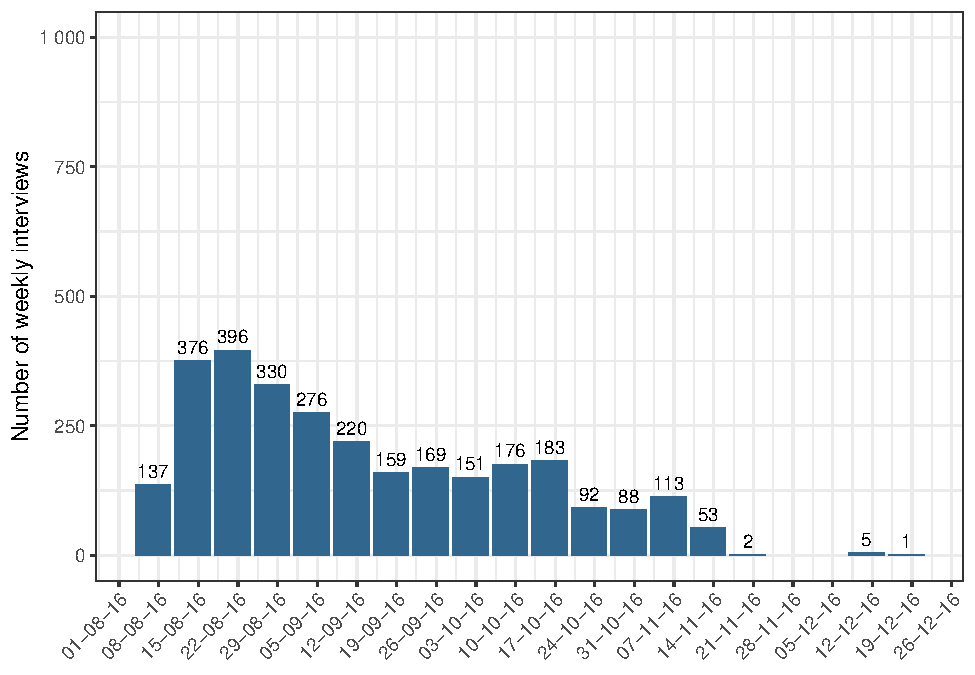
\includegraphics{methodological-manual-elsoc_files/figure-latex/graf-fechas-ola1-1} 

}

\caption{Number of weekly interviews, wave 2016}\label{fig:graf-fechas-ola1}
\end{figure}

\hypertarget{data-collection-indicators}{%
\paragraph*{Data collection indicators}\label{data-collection-indicators}}
\addcontentsline{toc}{paragraph}{Data collection indicators}

The following are the Response Rate 1 (RR1, as defined by AAPOR), Cooperation Rate 1 (COOP1), Refusal Rate 1 (REF1) and Contact Rate 1 (CON1)\footnote{For more information on the identification of case disposition codes and calculation of outcome rates, see \href{http://www.aapor.org/AAPOR_Main/media/publications/Standard-Definitions20169theditionfinal.pdf}{AAPOR (2016). Standard Definitions. Final Dispositions of Case Codes and Outcome Rates for Surveys}}

\begin{table}[H]

\caption{\label{tab:tabla-tasas-ola1}Response, Cooperation, Refusal and Contact Rates, wave 2016}
\centering
\begin{tabular}[t]{lc}
\toprule
Indicator & Original Sample\\
\midrule
Contact Rate & 72.6\%\\
Cooperation Rate & 86.0\%\\
Refusal Rate & 8.9\%\\
Response Rate & 62.4\%\\
\bottomrule
\end{tabular}
\end{table}

\hypertarget{casos-falsificados}{%
\paragraph*{Data correction for anomalous cases: 2016 and 2017 waves}\label{casos-falsificados}}
\addcontentsline{toc}{paragraph}{Data correction for anomalous cases: 2016 and 2017 waves}

In the context of executing the third wave of the ELSOC study (2018), we detected the falsification of a limited number of cases throughout the study in waves 2016 and 2017.

During the monitoring stage of the interviewers' work in 2018, the Microdata Center (CMD) detected and reported that a set of cases included in the panel sample were faked.

Due to the slow progress of ELSOC's 2018 field goals in Tarapacá and Valparaíso, they sent new interviewers and detected these problems. Specifically, they found systematically falsified surveys: conducted with different people than those included in the sample or where the interviewers requested information from third parties.

This led to an exhaustive review process, in which we detected 56 faked cases in the 2016 field and 47 in the 2017 field, concentrated in the regions of Tarapacá (11 cases in 2016 and 11 in 2017) and Valparaíso (45 cases in 2016 and 37 in 2017).

CMD's field strategy focuses on experienced interviewers, assigning the same cases to the interviewers over time, according to the recommendation of the specialized literature. The problem focused on some specific interviewers in those areas, which they did not detect during the field supervision of the first two waves.

The fake cases represent 1.9\% of the actual sample size of ELSOC 2016 (N = 2,984) and 1.9\% of 2017 (N = 2,522), so we consider them to have a marginal impact at the overall level. Despite this, we decided to exclude counterfeit cases from the databases, and to generate and make available a corrected version of the 2016 and 2017 databases. We fixed the weights considering the elimination of these cases.

To avoid these problems in the future, we modified the supervision protocols, increasing face-to-face oversight and the percentage of cases supervised per interviewer. In addition, we implemented an interviewer rotation system so that the same interviewers do not collect the sample in more than one round.

\hypertarget{wave-implementation-1}{%
\subsubsection{2017 Wave Implementation}\label{wave-implementation-1}}

Data collection was carried out over twelve weeks, between July and October 2017 (see Figure \ref{fig:graf-fechas-ola2}). 120 interviewers were distributed in the 17 work sites for the field implementation.

The field lasted a more extended period than predicted, as it was estimated to last nine weeks, finally extending to twelve. However, data collection was faster than the first wave, which lasted 20 weeks. This quicker time was due to the availability of contact information for the interviewers obtained in the previous wave.

The duration of the fieldwork over the original estimate responded to how challenging it was to contact the interviewees in the Metropolitan and Valparaíso regions.

The closure of the survey fieldwork took place once the entire sample was covered. We completed the fieldwork with 2,521 surveys conducted.

\begin{figure}

{\centering 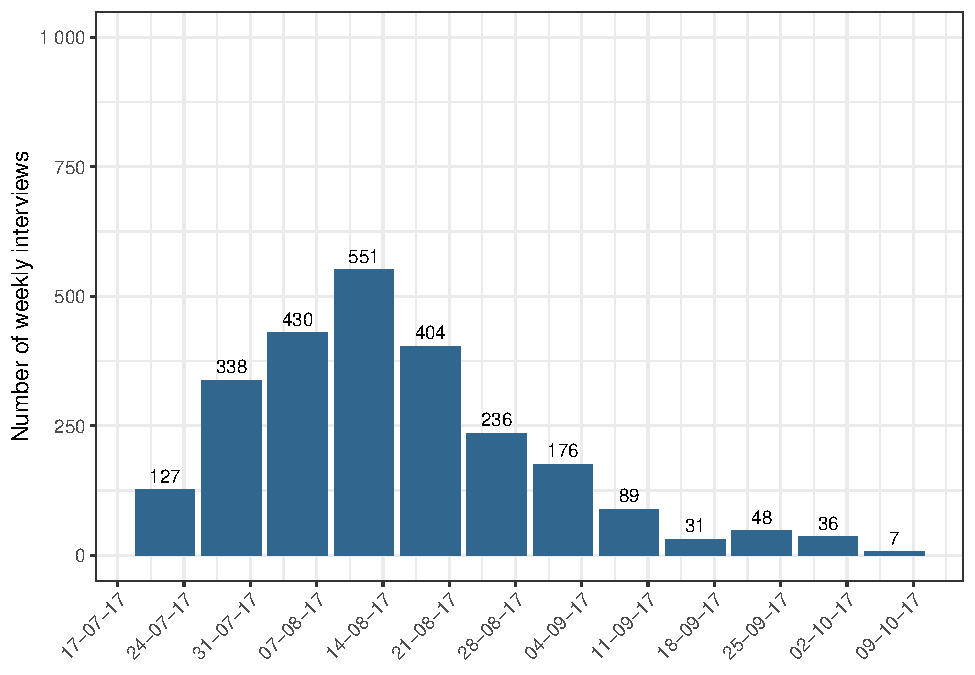
\includegraphics{methodological-manual-elsoc_files/figure-latex/graf-fechas-ola2-1} 

}

\caption{Number of weekly interviews, wave 2017}\label{fig:graf-fechas-ola2}
\end{figure}

\hypertarget{data-collection-indicators-1}{%
\paragraph*{Data collection indicators}\label{data-collection-indicators-1}}
\addcontentsline{toc}{paragraph}{Data collection indicators}

The following are the Response Rate 1 (RR1, as defined by AAPOR), Cooperation Rate 1 (COOP1), Refusal Rate 1 (REF1) and Contact Rate 1 (CON1):

\begin{table}[H]

\caption{\label{tab:tabla-tasas-ola2}Response, Cooperation, Refusal and Contact Rates, wave 2017}
\centering
\begin{tabular}[t]{lc}
\toprule
Indicator & Original Sample\\
\midrule
Contact Rate & 88.7\%\\
Cooperation Rate & 93.1\%\\
Refusal Rate & 6.0\%\\
Response Rate & 82.6\%\\
\bottomrule
\end{tabular}
\end{table}

\hypertarget{falsified-cases-in-wave-2017}{%
\paragraph{Falsified cases in wave 2017}\label{falsified-cases-in-wave-2017}}

After the procedures applied by the CMD in 2018, we found and corrected anomalies in surveys conducted in 2016 and 2017. For more details of the problem and its correction, see \protect\hyperlink{casos-falsificados}{Data correction for falsified cases: Waves 2016 and 2017}.

\hypertarget{wave-implementation-2}{%
\subsubsection{2018 Wave Implementation}\label{wave-implementation-2}}

We developed the fieldwork between August and December 2018, with an estimated time (15 weeks, approximately) (see Figure \ref{fig:graf-fechas-ola3}). There were 189 interviewers distributed in 18 work sites to execute the fieldwork.

We included the refreshment sample during this fieldwork, which generated a difficulty for the interviewers since they had to explain and motivate the participation of families and interviewees in the study.

On the other hand, interviewees of the follow-up sample (Original sample) of 2016-2017 had contact difficulties due to a higher presence of registered address changes than in previous versions of the survey. 6.9\% had moved to a different address.

Another challenge we faced in the wave is related to the fake cases detected (see \protect\hyperlink{casos-falsificados}{Data correction for fake cases: Waves 2016 and 2017}). This problem implied an exhaustive on-site review of these cases, while strengthening the control system, considering the following:

\begin{enumerate}
\def\labelenumi{\arabic{enumi}.}
\item
  Increase the percentage of surveys monitored from 10\% to 15\% in 2018. This ensures the control of at least 20\% of the work performed by each interviewer.
\item
  For future project waves, we defined a rotation of interviewers of the same interviewee.
\item
  Registration of the interviewers involved to avoid their consideration in future study applications. Regarding the general dynamics of the work, we created economic incentives for the interviewers to achieve the expected sample. Likewise, we arranged transport mechanisms for the interviewers to cover the entire sample on a schedule.
\end{enumerate}

The survey fieldwork ended with the agreement of COES once we covered the entire sample. The fieldwork closed with 2,274 surveys in the follow-up sample and 1,523 surveys in the refreshment sample.

\begin{figure}

{\centering 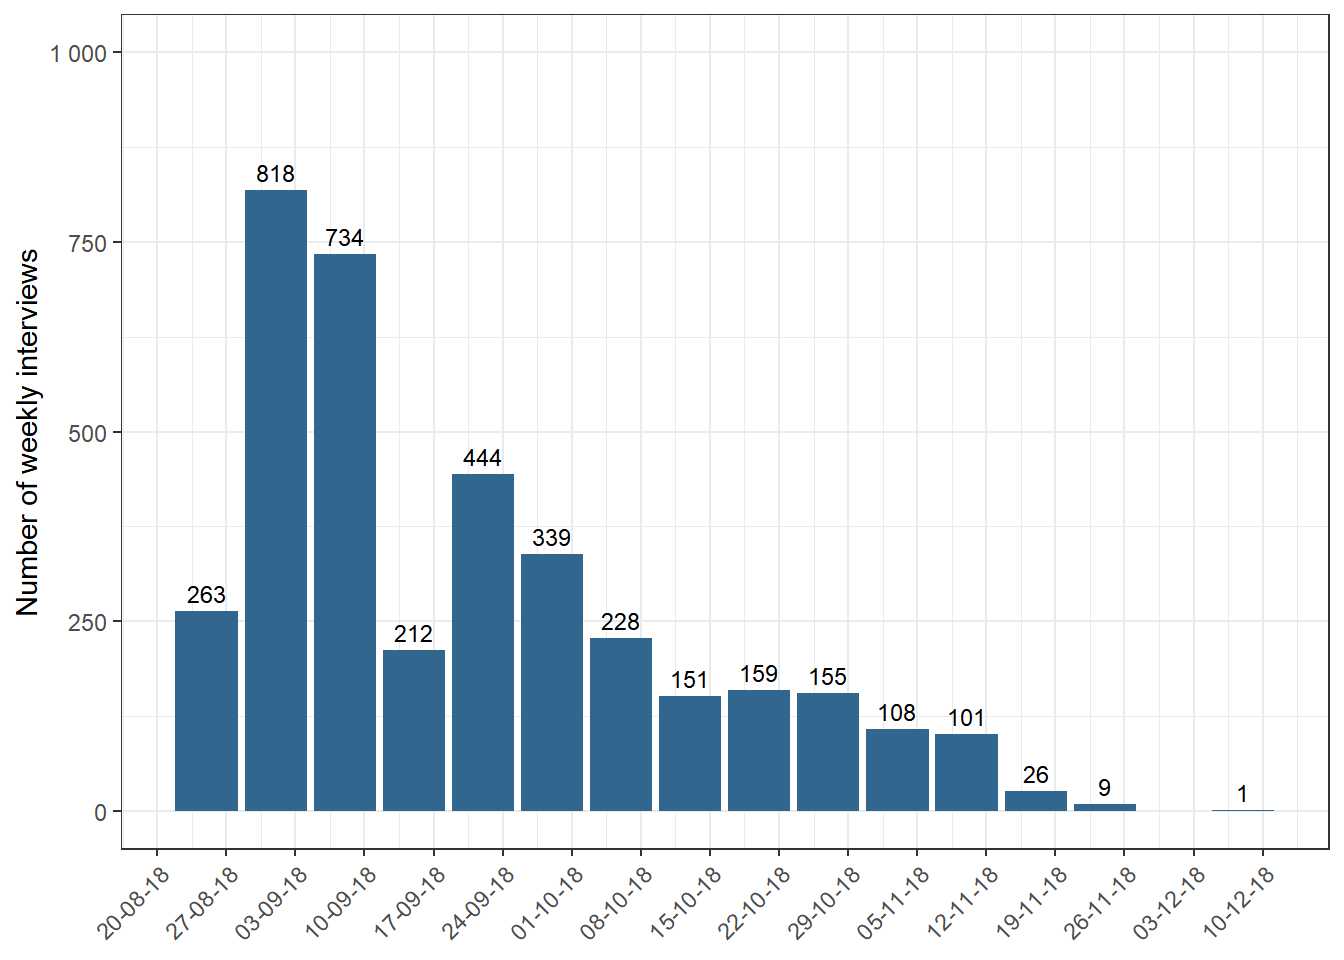
\includegraphics{methodological-manual-elsoc_files/figure-latex/graf-fechas-ola3-1} 

}

\caption{Number of weekly interviews, wave 2018}\label{fig:graf-fechas-ola3}
\end{figure}

\hypertarget{data-collection-indicators-2}{%
\paragraph*{Data collection indicators}\label{data-collection-indicators-2}}
\addcontentsline{toc}{paragraph}{Data collection indicators}

The following are the Response Rate 1 (RR1, as defined by AAPOR), Cooperation Rate 1 (COOP1), Refusal Rate 1 (REF1) and Contact Rate 1 (CON1):

\begin{table}[H]

\caption{\label{tab:tabla-tasas-ola3}Response, Cooperation, Refusal and Contact Rates, wave 2018}
\centering
\begin{tabular}[t]{lcc}
\toprule
Indicator & Original Sample & Refreshment Sample\\
\midrule
Contact Rate & 86.0\% & 66.0\%\\
Cooperation Rate & 93.0\% & 88.0\%\\
Refusal Rate & 5.0\% & 8.0\%\\
Response Rate & 80.0\% & 58.0\%\\
\bottomrule
\end{tabular}
\end{table}

\hypertarget{wave-implementation-3}{%
\subsubsection{2019 Wave Implementation}\label{wave-implementation-3}}

We scheduled ELSOC 2019 data collection to begin on Saturday, the 19th of October 2019. However, due to the Chilean Social Outburst that started on the 18th of October 2019, we suspended the fieldwork until Thursday, the 21st of November, when the data collection finally began. Therefore, we surveyed during the Social Outburst period, making its execution difficult.

The work lasted for 13 weeks (we decided to pause the data collection during the last three weeks of February 2020, given the exhaustion of the sample and the field team) (see Figure \ref{fig:graf-fechas-ola4}). There were 143 interviewers in the field, distributed in 16 work sites, administered by trained zone coordinators.

\begin{figure}

{\centering 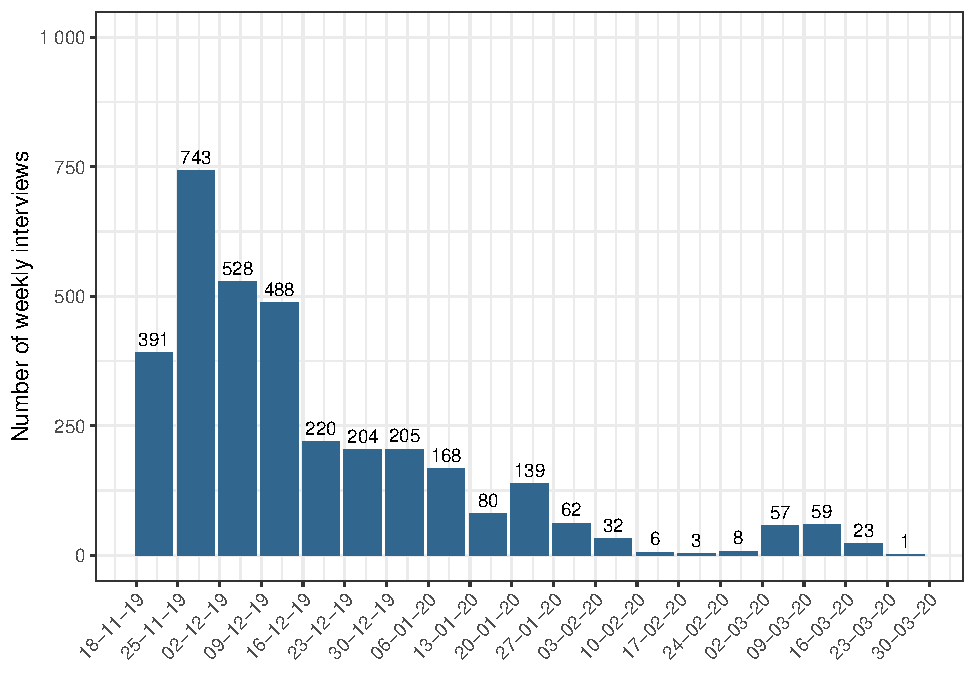
\includegraphics{methodological-manual-elsoc_files/figure-latex/graf-fechas-ola4-1} 

}

\caption{Number of weekly interviews, wave 2019}\label{fig:graf-fechas-ola4}
\end{figure}

\hypertarget{data-collection-indicators-3}{%
\paragraph*{Data collection indicators}\label{data-collection-indicators-3}}
\addcontentsline{toc}{paragraph}{Data collection indicators}

The following are the Response Rate 1 (RR1, as defined by AAPOR), Cooperation Rate 1 (COOP1), Refusal Rate 1 (REF1) and Contact Rate 1 (CON1):

\begin{table}[H]

\caption{\label{tab:tabla-tasas-ola4}Response, Cooperation, Refusal and Contact Rates, wave 2019}
\centering
\begin{tabular}[t]{lcc}
\toprule
Indicator & Original Sample & Refreshment Sample\\
\midrule
Contact Rate & 86.0\% & 87.0\%\\
Cooperation Rate & 93.0\% & 95.0\%\\
Refusal Rate & 5.0\% & 3.0\%\\
Response Rate & 80.0\% & 83.0\%\\
\bottomrule
\end{tabular}
\end{table}

\hypertarget{wave-implementation-4}{%
\subsubsection{2021 Wave Implementation}\label{wave-implementation-4}}

The health crisis caused by the COVID-19 pandemic and its associated restrictions implied changing the methodology of application of the survey from face-to-face to remote through a telephone survey (For more details, see \protect\hyperlink{instrumento-covid}{Questionnaire 2021: Survey during the COVID-19 Pandemic}). This change in collecting data introduced a tremendous logistical and operational challenge since ELSOC had surveyed in person since its origins.

The COVID-19 pandemic also affected the traditional ELSOC survey date, which we scheduled to begin in October 2020. However, the fifth wave survey started on January 30th, 2021, with the assignment of the sample to trained interviewers. The reasons for postponing the survey period were mainly waiting for more favourable sanitary and lockdown conditions that would allow a face-to-face survey (however, it soon became apparent that it was impossible to maintain the face-to-face modality). We extended the fieldwork until mid-June 2021. Nevertheless, we carried out most surveying between February and April 2021 (see Figure \ref{fig:graf-fechas-ola5}).

Due to sample attrition and the deterioration of the team of interviewers given unsuccessful contact attempts, we decided to change the application methodology per sampling unit in May. We formed a group of interviewers dedicated exclusively to reviewing the sample on a given working day.

\begin{figure}

{\centering 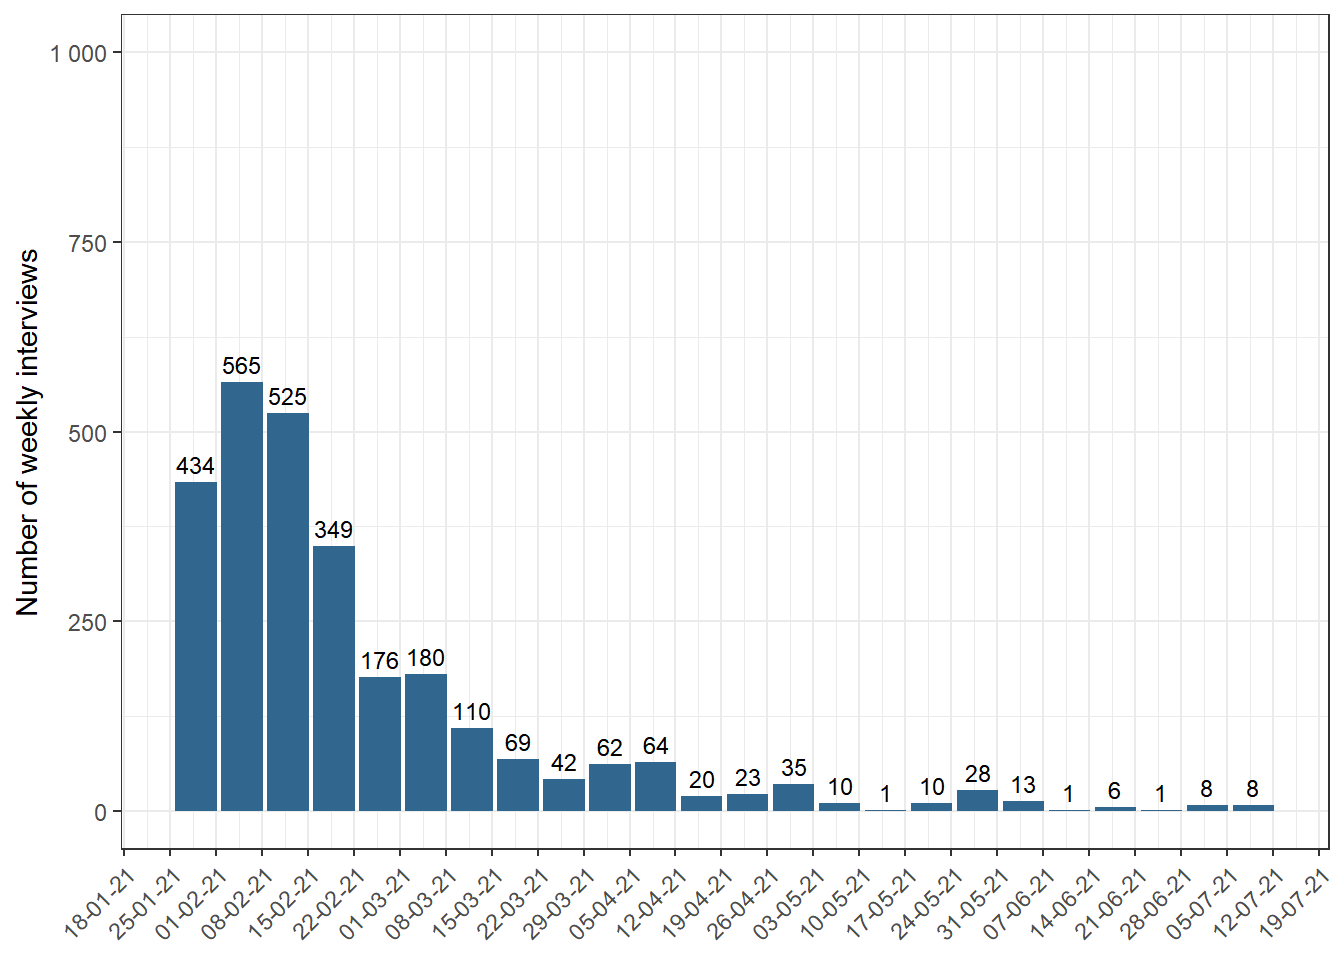
\includegraphics{methodological-manual-elsoc_files/figure-latex/graf-fechas-ola5-1} 

}

\caption{Number of weekly interviews, wave 2021}\label{fig:graf-fechas-ola5}
\end{figure}

\hypertarget{data-collection-indicators-4}{%
\paragraph*{Data collection indicators}\label{data-collection-indicators-4}}
\addcontentsline{toc}{paragraph}{Data collection indicators}

The following are the Response Rate 1 (RR1, as defined by AAPOR), Cooperation Rate 1 (COOP1), Refusal Rate 1 (REF1) and Contact Rate 1 (CON1):

\begin{table}[H]

\caption{\label{tab:tabla-tasas-ola5}Response, Cooperation, Refusal and Contact Rates, wave 2021}
\centering
\begin{tabular}[t]{lcc}
\toprule
Indicator & Original Sample & Refreshment Sample\\
\midrule
Contact Rate & 78.0\% & 87.3\%\\
Cooperation Rate & 83.7\% & 76.1\%\\
Refusal Rate & 11.0\% & 8.8\%\\
Response Rate & 65.2\% & 66.5\%\\
\bottomrule
\end{tabular}
\end{table}

\hypertarget{atricion}{%
\subsection{Survey Attrition}\label{atricion}}

The attrition of the sample is shown below:

\begin{table}[H]

\caption{\label{tab:tabla-atricion}Attrition of ELSOC samples between waves}
\centering
\begin{tabular}[t]{ccccc}
\toprule
\multicolumn{1}{c}{ } & \multicolumn{2}{c}{Achieved Sample} & \multicolumn{2}{c}{Attrition Rate} \\
\cmidrule(l{3pt}r{3pt}){2-3} \cmidrule(l{3pt}r{3pt}){4-5}
Measurement & Original Sample & Refreshment Sample & Original Sample & Refreshment Sample\\
\midrule
2016 & 2927 &  &  & \\
2017 & 2473 &  & 15.5\% & \\
2018 & 2229 & 1519 & 9.9\% & \\
2019 & 2153 & 1264 & 3.4\% & 16.8\%\\
2021 & 1739 & 1001 & 19.2\% & 20.8\%\\
\bottomrule
\end{tabular}
\end{table}

\begin{itemize}
\tightlist
\item
  By gender:
\end{itemize}

\begin{table}[H]

\caption{\label{tab:tabla-atricion-genero}Attrition of ELSOC samples between waves, by gender}
\centering
\begin{tabular}[t]{ccccc}
\toprule
\multicolumn{1}{c}{ } & \multicolumn{2}{c}{Achieved Sample} & \multicolumn{2}{c}{Attrition Rate} \\
\cmidrule(l{3pt}r{3pt}){2-3} \cmidrule(l{3pt}r{3pt}){4-5}
Measurement & Male & Female & Male & Female\\
\midrule
\addlinespace[0.3em]
\multicolumn{5}{l}{\textbf{Original Sample}}\\
\hspace{1em}2016 & 1163 & 1764 &  & \\
\hspace{1em}2017 & 953 & 1520 & 18.1\% & 13.8\%\\
\hspace{1em}2018 & 841 & 1387 & 11.8\% & 8.8\%\\
\hspace{1em}2019 & 807 & 1346 & 4.0\% & 3.0\%\\
\hspace{1em}2021 & 631 & 1108 & 21.8\% & 17.7\%\\
\addlinespace[0.3em]
\multicolumn{5}{l}{\textbf{Refreshment Sample}}\\
\hspace{1em}2018 & 607 & 912 &  & \\
\hspace{1em}2019 & 482 & 782 & 20.6\% & 14.3\%\\
\hspace{1em}2021 & 378 & 623 & 21.6\% & 20.3\%\\
\bottomrule
\end{tabular}
\end{table}

\begin{itemize}
\tightlist
\item
  By age segment:
\end{itemize}

\begin{table}[H]

\caption{\label{tab:tabla-atricion-edad}Attrition of ELSOC samples between waves, by age segment}
\centering
\begin{tabular}[t]{ccccccccc}
\toprule
\multicolumn{1}{c}{ } & \multicolumn{4}{c}{Achieved Sample} & \multicolumn{4}{c}{Attrition Sample} \\
\cmidrule(l{3pt}r{3pt}){2-5} \cmidrule(l{3pt}r{3pt}){6-9}
Measurement & 19-29 & 30-49 & 50-64 & 65 or over & 19-29 & 30-49 & 50-64 & 65 or over\\
\midrule
\addlinespace[0.3em]
\multicolumn{9}{l}{\textbf{Original Sample}}\\
\hspace{1em}2016 & 506 & 1157 & 839 & 425 &  &  &  & \\
\hspace{1em}2017 & 407 & 962 & 734 & 370 & 19.6\% & 16.9\% & 12.5\% & 12.9\%\\
\hspace{1em}2018 & 340 & 863 & 687 & 338 & 16.5\% & 10.3\% & 6.4\% & 8.6\%\\
\hspace{1em}2019 & 327 & 838 & 666 & 322 & 3.8\% & 2.9\% & 3.1\% & 4.7\%\\
\hspace{1em}2021 & 269 & 685 & 546 & 239 & 17.7\% & 18.3\% & 18.0\% & 25.8\%\\
\addlinespace[0.3em]
\multicolumn{9}{l}{\textbf{Refreshment Sample}}\\
\hspace{1em}2018 & 341 & 579 & 418 & 181 &  &  &  & \\
\hspace{1em}2019 & 271 & 472 & 369 & 152 & 20.5\% & 18.5\% & 11.7\% & 16.0\%\\
\hspace{1em}2021 & 216 & 391 & 282 & 112 & 20.3\% & 17.2\% & 23.6\% & 26.3\%\\
\bottomrule
\end{tabular}
\end{table}

\begin{itemize}
\tightlist
\item
  By educational level:
\end{itemize}

\begin{table}[H]

\caption{\label{tab:tabla-atricion-educ}Attrition of ELSOC samples between waves, by educational level}
\centering
\begin{tabular}[t]{ccccccccc}
\toprule
\multicolumn{1}{c}{ } & \multicolumn{4}{c}{Achieved Sample} & \multicolumn{4}{c}{Attrition Rate} \\
\cmidrule(l{3pt}r{3pt}){2-5} \cmidrule(l{3pt}r{3pt}){6-9}
Measurement & Primary & Secondary & Technical & University & Primary & Secondary & Technical & University\\
\midrule
\addlinespace[0.3em]
\multicolumn{9}{l}{\textbf{Original Sample}}\\
\hspace{1em}2016 & 656 & 1251 & 483 & 535 &  &  &  & \\
\hspace{1em}2017 & 580 & 1062 & 396 & 434 & 11.6\% & 15.1\% & 18.0\% & 18.9\%\\
\hspace{1em}2018 & 512 & 977 & 358 & 380 & 11.7\% & 8.0\% & 9.6\% & 12.4\%\\
\hspace{1em}2019 & 490 & 953 & 341 & 368 & 4.3\% & 2.5\% & 4.7\% & 3.2\%\\
\hspace{1em}2021 & 363 & 757 & 283 & 336 & 25.9\% & 20.6\% & 17.0\% & 8.7\%\\
\addlinespace[0.3em]
\multicolumn{9}{l}{\textbf{Refreshment Sample}}\\
\hspace{1em}2018 & 283 & 633 & 253 & 347 &  &  &  & \\
\hspace{1em}2019 & 254 & 537 & 206 & 264 & 10.2\% & 15.2\% & 18.6\% & 23.9\%\\
\hspace{1em}2021 & 167 & 426 & 175 & 233 & 34.3\% & 20.7\% & 15.0\% & 11.7\%\\
\bottomrule
\end{tabular}
\end{table}

\newpage

\hypertarget{bases-datos}{%
\section{Databases}\label{bases-datos}}

\hypertarget{databases-download}{%
\subsection{Databases Download}\label{databases-download}}

After completing the review and validation process, ELSOC databases are made available to the general public. The databases are published and saved in the \textbf{Harvard Dataverse} repository in the \href{https://dataverse.harvard.edu/dataverse/coes_data_repository}{COES data folder}. This repository allows free and secure access to the databases.

ELSOC is available as cross-sectional databases by wave: waves 2016, 2017, 2018, 2019 and 2021, in R (.RData), SPSS (.sav), Stata 13 (.dta) and Stata 14 (.dta) data formats.

Since 2019, we have published the databases in a longitudinal form to facilitate their use as a panel survey. We share the longitudinal database 2016-2019 in wide format and the longitudinal database 2016-2021 in wide and long structures. We harmonized the variables that have changed over time to allow their longitudinal use.

As part of a continuous improvement process, we might update published databases during the development of ELSOC, due to correction of potential bugs, improvements in data formatting, updating of non-response codes, etc. Therefore, we publish the latest available version in the Harvard Dataverse repository, as well as all previous versions needed.

\hypertarget{technical-report}{%
\subsection{Technical Report}\label{technical-report}}

This section presents the technical report. See Table \ref{tab:ficha}, which summarizes the main characteristics of ELSOC:

\begin{longtable}[t]{>{\raggedright\arraybackslash}p{8em}>{\raggedright\arraybackslash}p{35em}}
\caption{\label{tab:ficha}ELSOC-COES Technical Report}\\
\toprule
Characteristics & ELSOC\\
\midrule
\endfirsthead
\caption[]{\label{tab:ficha}ELSOC-COES Technical Report \textit{(continued)}}\\
\toprule
Characteristics & ELSOC\\
\midrule
\endhead

\endfoot
\bottomrule
\endlastfoot
Objective & To analyze longitudinally the evolution of conflict and cohesion in Chilean society\\
Design & Quantitative study through a structured questionnaire\\
Instrument & The questionnaire is composed of single and multiple closed questions and some open questions. It combines permanent (all waves) and interleaved questions\\
Topic features & It contains seven thematic modules: Territory, Social networks and attitudes, Citizenship and democracy, Inequality and legitimacy, Social conflict, Health and well-being, and Sociodemographic characterization\\
Unit of analysis & Individuals\\
\addlinespace
Target population & Men and women between 18 and 75 years old, residents of occupied private households, located in 40 cities (92 communes) of the country\\
Sampling frame & Sampling frame of blocks of the 2011 pre-census, prepared by the Territorial Intelligence Center (CIT) of the Adolfo Ibáñez University\\
Sample design & Probabilistic, stratified, clustered and multistage.\\
Sample unit & First cities are selected (UPM), then blocks (USM), sub-blocks and households (UTM). The last selection unit are individuals\\
Frequency & Annually. Refreshment sample in the 3rd year\\
\addlinespace
Surveying mode & Face-to-face survey in the interviewees household. Personal interview applied by an interviewer using a tablet (CAPI system: Computer-assisted personal interviewing)\\
Informant & Male or female resident in the household, between 18 and 75 years old\\
Ethic aspects & Voluntary interview. Contact information of interviewees is requested, but is not accessible (confidential). Geo-referenced information is also kept confidential. Public access database\\
Average duration & 51 minutes\\
Representativeness & Approximately 77\% of the countrys population and 93\% of the urban population in wave 2016\\
\addlinespace
Responsible entity & Centre for Social Conflict and Cohesion Studies (COES)\\
Executing entity & Consultant Stephanie Eckman and Centro de Inteligencia Territorial (CIT) of Adolfo Ibáñez University (sample design). MicroData Center (CMD) of the University of Chile (collection, data processing and construction of expansion factors)\\*
\end{longtable}

\hypertarget{database-usage-protocol}{%
\subsection{Database Usage Protocol}\label{database-usage-protocol}}

Any publication using ELSOC databases, in any of their versions, must cite the source in the following ways (depending on the database used):

\begin{itemize}
\tightlist
\item
  ELSOC 2016:
\end{itemize}

\textbf{Centre for Social Conflict and Cohesion Studies. (2016). Chilean Longitudinal Social Survey, First Wave (ELSOC\_W01\_v1.00). {[}Database{]}. Santiago, Chile: Centre for Social Conflict and Cohesion Studies (COES). www.coes.cl}

\begin{itemize}
\tightlist
\item
  ELSOC 2017:
\end{itemize}

\textbf{Centre for Social Conflict and Cohesion Studies. (2017). Chilean Longitudinal Social Survey, Second Wave (ELSOC\_W02\_v1.00). {[}Database{]}. Santiago, Chile: Centre for Social Conflict and Cohesion Studies (COES). www.coes.cl}

\begin{itemize}
\tightlist
\item
  ELSOC 2018:
\end{itemize}

\textbf{Centre for Social Conflict and Cohesion Studies. (2018). Chilean Longitudinal Social Survey, Third Wave (ELSOC\_W03\_v1.00). {[}Database{]}. Santiago, Chile: Centre for Social Conflict and Cohesion Studies (COES). www.coes.cl}

\begin{itemize}
\tightlist
\item
  ELSOC 2019:
\end{itemize}

\textbf{Centre for Social Conflict and Cohesion Studies. (2019). Chilean Longitudinal Social Survey, Fourth Wave (ELSOC\_W04\_v1.00). {[}Database{]}. Santiago, Chile: Centre for Social Conflict and Cohesion Studies (COES). www.coes.cl}

\begin{itemize}
\tightlist
\item
  ELSOC 2021:
\end{itemize}

\textbf{Centre for Social Conflict and Cohesion Studies. (2021). Chilean Longitudinal Social Survey, Fifth Wave (ELSOC\_W05\_v1.00). {[}Database{]}. Santiago, Chile: Centre for Social Conflict and Cohesion Studies (COES). www.coes.cl}

Or in its longitudinal format:

\textbf{Centre for Social Conflict and Cohesion Studies. (2021). Chilean Longitudinal Social Survey, Combined Panel Version 2016-2019 (ELSOC\_Wide\_2016\_2019\_v1.00). {[}Database{]}. Santiago, Chile: Centre for Social Conflict and Cohesion Studies (COES). www.coes.cl}

Finally, if you wish to cite this User's Manual:

**Centre for Social Conflict and Cohesion Studies. (2021). Chilean Longitudinal Social Survey User's Manual. Santiago, Chile: Centre for Social Conflict and Cohesion Studies (COES).*

**

Centro de Estudios de Conflicto y Cohesión Social (2021). Estudio Longitudinal Social de Chile, Quinta Ola (ELSOC\_W05\_v1.00). {[}Archivo de datos{]}. Santiago, Chile: Centro de Estudios de Conflicto y Cohesión Social (COES). www.coes.cl

\newpage

\hypertarget{ethics}{%
\section{Ethics}\label{ethics}}

\hypertarget{ethics-committee-approval}{%
\subsection{Ethics Committee Approval}\label{ethics-committee-approval}}

The Chilean Longitudinal Social Survey (ELSOC) has ethical approval in all its waves from the \href{http://eticayseguridad.uc.cl/comite-etico-cientifico-en-ciencias-sociales-artes-y-humanidades.html}{Scientific Ethical Committee of Social Sciences, Arts and Humanities of the Pontifical Catholic University of Chile} starting on June 8th, 2016, with \textbf{Protocol ID 160129004}.

The Ethics Committee's approval was renewed on January 6th, 2021.

\hypertarget{informed-consent}{%
\subsection{Informed consent}\label{informed-consent}}

Study participants signed a Written Informed Consent Form detailing the study's objectives, the extent of their participation, how the study will be carried out, and how the information and data provided will be stored.

Study participants in the Original Sample signed the Informed Consent in 2016, while participants from the Refreshment Sample signed it in 2018. Additionally, due to the change in modality made during the 2021 wave survey (see \protect\hyperlink{instrumento-covid}{Questionnaire 2021: survey during the COVID-19 pandemic}), participants in both samples were asked to sign an Appendix to the Informed Consent, detailing the changes made during that wave.

\newpage

\hypertarget{questions-and-queries}{%
\section{Questions and Queries}\label{questions-and-queries}}

In case you detect problems with the database, wish to make requests and/or have queries about aspects not covered by this User's Manual, which cannot be solved by other means, you can contact the COES Survey Team at \url{encuestacoes@gmail.com}. The team will process your request and will try to respond as soon as possible.

\newpage

\hypertarget{libro-codigos}{%
\section{Codebook}\label{libro-codigos}}

For proper use of the ELSOC COES database, we recommend that researchers work with the codebook presented below. This section shows the longitudinal code of each variable; the associated variable label; the phrasing of each preamble, question and item; the different response categories and associated codes; and observations on the variables that have undergone modifications throughout the measurements of the study. In addition, we include frequency tables for each question according to wave and sample (we omitted continuous and text variables).

We designed the codebook to summarize all relevant information about the variables in the database into a standard format for ease of use. Generally, the variables included in the database take the following form:

\begin{quote}
\textbf{Longitudinal Code}. Variable label

\emph{Question phrasing}

\emph{Response Codes of response categories}

Notes

Frequency table
\end{quote}

We present the questions by questionnaire module to facilitate the understanding.

The Longitudinal Code is associated with each questionnaire item in the database and codebook. Through these codes, we can identify different items. In the wide form longitudinal database, the code includes *\_w01\emph{, }\_w02\emph{, }\_w03\emph{, }\_w04* or *\_w05* at the end to denote whether the variable corresponds to waves 2016, 2017, 2018, 2019 or 2021, respectively.

We included variable labels in the Codebook and the databases. The ELSOC team designed them intending to briefly describe the phenomenon or dimension to be measured\footnote{We eliminated accents and other symbols not included in all statistical software (e.g.~accents and ñ)}. The question's phrasing follows the labels, including preambles, response codes and categories. In constructing the database, we entered response codes as numerical values and response categories as labels.

Finally, we included observations associated with possible changes over time or aspects to be considered when using the variables.

The string variables (text) do not present codes since they are literal verbal responses of the interviewers. There are no response categories in items where we request a numerical answer because we record the value indicated by the respondent.

\hypertarget{citizenship-and-democracy-module}{%
\subsection{Citizenship and Democracy Module}\label{citizenship-and-democracy-module}}

\begin{itemize}
\tightlist
\item
  \textbf{c01}: Satisfaction with democracy in Chile
\end{itemize}

\begin{quote}
\emph{How satisfied are you with the way democracy works in Chile?}.
\end{quote}

\begin{quote}
-999 No Answer (do not read)\\
-888 Don't Know (do not read)\\
-777 Value lost due to technical error\\
-666 Value lost due to incomplete survey\\
1 Completely dissatisfied\\
2 Dissatisfied\\
3 Neither satisfied nor dissatisfied\\
4 Satisfied\\
5 Completely satisfied
\end{quote}

\begin{table}[H]
\begin{tabular}[t]{lccccc}
\toprule
c01 & 2016 & 2017 & 2018 & 2019 & 2021\\
\midrule
\addlinespace[0.3em]
\multicolumn{6}{l}{\textbf{Original Sample}}\\
\hspace{1em}-999 & 22 & 20 & 16 & 14 & 5\\
\hspace{1em}-888 & 107 & 98 & 102 & 46 & 18\\
\hspace{1em}-666 & 0 & 0 & 0 & 0 & 0\\
\hspace{1em}1 & 1228 & 866 & 616 & 1117 & 553\\
\hspace{1em}2 & 704 & 651 & 598 & 587 & 606\\
\hspace{1em}3 & 591 & 558 & 619 & 282 & 446\\
\hspace{1em}4 & 202 & 231 & 234 & 78 & 94\\
\hspace{1em}5 & 73 & 49 & 44 & 29 & 17\\
\addlinespace[0.3em]
\multicolumn{6}{l}{\textbf{Refreshment Sample}}\\
\hspace{1em}-999 & 0 & 0 & 17 & 6 & 3\\
\hspace{1em}-888 & 0 & 0 & 72 & 32 & 10\\
\hspace{1em}-666 & 0 & 0 & 0 & 0 & 8\\
\hspace{1em}1 & 0 & 0 & 446 & 669 & 295\\
\hspace{1em}2 & 0 & 0 & 438 & 329 & 373\\
\hspace{1em}3 & 0 & 0 & 361 & 181 & 236\\
\hspace{1em}4 & 0 & 0 & 147 & 31 & 64\\
\hspace{1em}5 & 0 & 0 & 38 & 16 & 12\\
\bottomrule
\end{tabular}
\end{table}

\begin{itemize}
\tightlist
\item
  \textbf{c02}: Generalized Social Trust
\end{itemize}

\begin{quote}
\emph{Generally speaking, would you say that most people can be trusted or that you have to be careful when dealing with them?}.
\end{quote}

\begin{quote}
-999 No Answer (do not read)\\
-888 Don't Know (do not read)\\
-777 Value lost due to technical error\\
-666 Value lost due to incomplete survey\\
1 Most people can be trusted\\
2 Have to be careful when dealing with people\\
3 It depends (don't read)
\end{quote}

\begin{table}[H]
\begin{tabular}[t]{lccccc}
\toprule
c02 & 2016 & 2017 & 2018 & 2019 & 2021\\
\midrule
\addlinespace[0.3em]
\multicolumn{6}{l}{\textbf{Original Sample}}\\
\hspace{1em}-999 & 12 & 2 & 5 & 0 & 0\\
\hspace{1em}-888 & 34 & 30 & 7 & 2 & 0\\
\hspace{1em}-666 & 0 & 0 & 0 & 0 & 0\\
\hspace{1em}1 & 276 & 272 & 231 & 214 & 131\\
\hspace{1em}2 & 2373 & 1987 & 1840 & 1850 & 1579\\
\hspace{1em}3 & 232 & 182 & 146 & 87 & 29\\
\addlinespace[0.3em]
\multicolumn{6}{l}{\textbf{Refreshment Sample}}\\
\hspace{1em}-999 & 0 & 0 & 3 & 0 & 0\\
\hspace{1em}-888 & 0 & 0 & 10 & 2 & 1\\
\hspace{1em}-666 & 0 & 0 & 0 & 0 & 8\\
\hspace{1em}1 & 0 & 0 & 156 & 109 & 75\\
\hspace{1em}2 & 0 & 0 & 1256 & 1091 & 880\\
\hspace{1em}3 & 0 & 0 & 94 & 62 & 37\\
\bottomrule
\end{tabular}
\end{table}

\begin{itemize}
\tightlist
\item
  \textbf{c03}: Generalized Social Altruism
\end{itemize}

\begin{quote}
\emph{Would you say that people, most of the time, try to help others, or are they concerned only with themselves?}.
\end{quote}

\begin{quote}
-999 No Answer (do not read)\\
-888 Don't Know (do not read)\\
-777 Value lost due to technical error\\
-666 Value lost due to incomplete survey\\
1 Most of the time they try to help others\\
2 Most of the time they only care about themselves\\
3 It depends (do not read)
\end{quote}

\begin{table}[H]
\begin{tabular}[t]{lccccc}
\toprule
c03 & 2016 & 2017 & 2018 & 2019 & 2021\\
\midrule
\addlinespace[0.3em]
\multicolumn{6}{l}{\textbf{Original Sample}}\\
\hspace{1em}-999 & 9 & 2 & 4 & 0 & 0\\
\hspace{1em}-888 & 24 & 21 & 11 & 5 & 3\\
\hspace{1em}-666 & 0 & 0 & 0 & 0 & 0\\
\hspace{1em}1 & 414 & 472 & 390 & 413 & 324\\
\hspace{1em}2 & 2196 & 1753 & 1611 & 1611 & 1302\\
\hspace{1em}3 & 284 & 225 & 213 & 124 & 110\\
\addlinespace[0.3em]
\multicolumn{6}{l}{\textbf{Refreshment Sample}}\\
\hspace{1em}-999 & 0 & 0 & 1 & 0 & 0\\
\hspace{1em}-888 & 0 & 0 & 8 & 3 & 2\\
\hspace{1em}-666 & 0 & 0 & 0 & 0 & 8\\
\hspace{1em}1 & 0 & 0 & 240 & 269 & 177\\
\hspace{1em}2 & 0 & 0 & 1128 & 913 & 739\\
\hspace{1em}3 & 0 & 0 & 142 & 79 & 75\\
\bottomrule
\end{tabular}
\end{table}

\begin{itemize}
\tightlist
\item
  \textbf{c04}: Most people try to be fair
\end{itemize}

\begin{quote}
\emph{Do you think most people would try to take advantage of you if they had the opportunity, or do you think they would try to be fair?}.
\end{quote}

\begin{quote}
-999 No Answer (do not read)\\
-888 Don't Know (do not read)\\
-777 Value lost due to technical error\\
-666 Value lost due to incomplete survey\\
1 Most people would try to take advantage\\
2 Most people would try to be fair\\
3 It depends (do not read)
\end{quote}

\begin{table}[H]
\begin{tabular}[t]{lccccc}
\toprule
c04 & 2016 & 2017 & 2018 & 2019 & 2021\\
\midrule
\addlinespace[0.3em]
\multicolumn{6}{l}{\textbf{Original Sample}}\\
\hspace{1em}-999 & 14 & 3 & 4 & 1 & 1\\
\hspace{1em}-888 & 44 & 36 & 27 & 27 & 10\\
\hspace{1em}-666 & 0 & 0 & 0 & 0 & 0\\
\hspace{1em}1 & 1797 & 1350 & 1287 & 1286 & 1107\\
\hspace{1em}2 & 723 & 787 & 641 & 653 & 513\\
\hspace{1em}3 & 349 & 297 & 270 & 186 & 108\\
\addlinespace[0.3em]
\multicolumn{6}{l}{\textbf{Refreshment Sample}}\\
\hspace{1em}-999 & 0 & 0 & 5 & 1 & 0\\
\hspace{1em}-888 & 0 & 0 & 17 & 12 & 9\\
\hspace{1em}-666 & 0 & 0 & 0 & 0 & 8\\
\hspace{1em}1 & 0 & 0 & 899 & 717 & 606\\
\hspace{1em}2 & 0 & 0 & 420 & 407 & 311\\
\hspace{1em}3 & 0 & 0 & 178 & 127 & 67\\
\bottomrule
\end{tabular}
\end{table}

\begin{itemize}
\tightlist
\item
  \textbf{c05\_01}: Level of confidence: Government
\end{itemize}

\begin{quote}
\emph{Using a scale where 1 represents ``Not at all'' and 5 ``A lot'', can you tell me how much confidence you have in each of the following institutions?}: \emph{Government}.
\end{quote}

\begin{quote}
-999 No Answer (do not read)\\
-888 Don't Know (do not read)\\
-777 Value lost due to technical error\\
-666 Value lost due to incomplete survey\\
1 Not at all\\
2 A little\\
3 Some\\
4 Quite\\
5 A lot
\end{quote}

\begin{table}[H]
\begin{tabular}[t]{lccccc}
\toprule
c05\_01 & 2016 & 2017 & 2018 & 2019 & 2021\\
\midrule
\addlinespace[0.3em]
\multicolumn{6}{l}{\textbf{Original Sample}}\\
\hspace{1em}-999 & 1 & 3 & 4 & 4 & 3\\
\hspace{1em}-888 & 11 & 9 & 10 & 5 & 0\\
\hspace{1em}-666 & 0 & 0 & 0 & 0 & 0\\
\hspace{1em}1 & 1363 & 1019 & 655 & 1284 & 659\\
\hspace{1em}2 & 808 & 741 & 655 & 497 & 630\\
\hspace{1em}3 & 554 & 510 & 655 & 282 & 364\\
\hspace{1em}4 & 153 & 155 & 199 & 63 & 68\\
\hspace{1em}5 & 37 & 36 & 51 & 18 & 15\\
\addlinespace[0.3em]
\multicolumn{6}{l}{\textbf{Refreshment Sample}}\\
\hspace{1em}-999 & 0 & 0 & 5 & 2 & 0\\
\hspace{1em}-888 & 0 & 0 & 6 & 1 & 2\\
\hspace{1em}-666 & 0 & 0 & 0 & 0 & 8\\
\hspace{1em}1 & 0 & 0 & 497 & 754 & 384\\
\hspace{1em}2 & 0 & 0 & 429 & 311 & 357\\
\hspace{1em}3 & 0 & 0 & 397 & 157 & 196\\
\hspace{1em}4 & 0 & 0 & 152 & 32 & 45\\
\hspace{1em}5 & 0 & 0 & 33 & 7 & 9\\
\bottomrule
\end{tabular}
\end{table}

\begin{itemize}
\tightlist
\item
  \textbf{c05\_02}: Level of confidence: Political Parties
\end{itemize}

\begin{quote}
\emph{Using a scale where 1 represents ``Not at all'' and 5 ``A lot'', can you tell me how much confidence you have in each of the following institutions?}: \emph{Political Parties}.
\end{quote}

\begin{quote}
-999 No Answer (do not read)\\
-888 Don't Know (do not read)\\
-777 Value lost due to technical error\\
-666 Value lost due to incomplete survey\\
1 Not at all\\
2 A little\\
3 Some\\
4 Quite\\
5 A lot
\end{quote}

\begin{table}[H]
\begin{tabular}[t]{lccccc}
\toprule
c05\_02 & 2016 & 2017 & 2018 & 2019 & 2021\\
\midrule
\addlinespace[0.3em]
\multicolumn{6}{l}{\textbf{Original Sample}}\\
\hspace{1em}-999 & 7 & 5 & 6 & 8 & 4\\
\hspace{1em}-888 & 14 & 15 & 21 & 9 & 7\\
\hspace{1em}-666 & 0 & 0 & 0 & 0 & 0\\
\hspace{1em}1 & 2080 & 1667 & 1378 & 1711 & 1190\\
\hspace{1em}2 & 557 & 532 & 521 & 310 & 398\\
\hspace{1em}3 & 244 & 219 & 274 & 99 & 128\\
\hspace{1em}4 & 20 & 26 & 25 & 13 & 10\\
\hspace{1em}5 & 5 & 9 & 4 & 3 & 2\\
\addlinespace[0.3em]
\multicolumn{6}{l}{\textbf{Refreshment Sample}}\\
\hspace{1em}-999 & 0 & 0 & 4 & 3 & 0\\
\hspace{1em}-888 & 0 & 0 & 10 & 3 & 3\\
\hspace{1em}-666 & 0 & 0 & 0 & 0 & 8\\
\hspace{1em}1 & 0 & 0 & 974 & 985 & 663\\
\hspace{1em}2 & 0 & 0 & 336 & 218 & 247\\
\hspace{1em}3 & 0 & 0 & 178 & 50 & 78\\
\hspace{1em}4 & 0 & 0 & 14 & 5 & 1\\
\hspace{1em}5 & 0 & 0 & 3 & 0 & 1\\
\bottomrule
\end{tabular}
\end{table}

\begin{itemize}
\tightlist
\item
  \textbf{c05\_03}: Level of confidence: Police
\end{itemize}

\begin{quote}
\emph{Using a scale where 1 represents ``Not at all'' and 5 ``A lot'', can you tell me how much confidence you have in each of the following institutions?}: \emph{Police}.
\end{quote}

\begin{quote}
-999 No Answer (do not read)\\
-888 Don't Know (do not read)\\
-777 Value lost due to technical error\\
-666 Value lost due to incomplete survey\\
1 Not at all\\
2 A little\\
3 Some\\
4 Quite\\
5 A lot
\end{quote}

\begin{table}[H]
\begin{tabular}[t]{lccccc}
\toprule
c05\_03 & 2016 & 2017 & 2018 & 2019 & 2021\\
\midrule
\addlinespace[0.3em]
\multicolumn{6}{l}{\textbf{Original Sample}}\\
\hspace{1em}-999 & 1 & 1 & 2 & 2 & 2\\
\hspace{1em}-888 & 3 & 6 & 3 & 3 & 1\\
\hspace{1em}-666 & 0 & 0 & 0 & 0 & 0\\
\hspace{1em}1 & 376 & 408 & 266 & 680 & 337\\
\hspace{1em}2 & 480 & 481 & 429 & 493 & 486\\
\hspace{1em}3 & 883 & 721 & 700 & 518 & 490\\
\hspace{1em}4 & 914 & 657 & 665 & 320 & 299\\
\hspace{1em}5 & 270 & 199 & 164 & 137 & 124\\
\addlinespace[0.3em]
\multicolumn{6}{l}{\textbf{Refreshment Sample}}\\
\hspace{1em}-999 & 0 & 0 & 2 & 0 & 0\\
\hspace{1em}-888 & 0 & 0 & 1 & 3 & 0\\
\hspace{1em}-666 & 0 & 0 & 0 & 0 & 8\\
\hspace{1em}1 & 0 & 0 & 196 & 426 & 205\\
\hspace{1em}2 & 0 & 0 & 301 & 288 & 321\\
\hspace{1em}3 & 0 & 0 & 487 & 283 & 255\\
\hspace{1em}4 & 0 & 0 & 406 & 179 & 162\\
\hspace{1em}5 & 0 & 0 & 126 & 85 & 50\\
\bottomrule
\end{tabular}
\end{table}

\begin{itemize}
\tightlist
\item
  \textbf{c05\_04}: Level of confidence: Unions
\end{itemize}

\begin{quote}
\emph{Using a scale where 1 represents ``Not at all'' and 5 ``A lot'', can you tell me how much confidence you have in each of the following institutions?}: \emph{Unions}.
\end{quote}

\begin{quote}
-999 No Answer (do not read)\\
-888 Don't Know (do not read)\\
-777 Value lost due to technical error\\
-666 Value lost due to incomplete survey\\
1 Not at all\\
2 A little\\
3 Some\\
4 Quite\\
5 A lot
\end{quote}

\begin{table}[H]
\begin{tabular}[t]{lccccc}
\toprule
c05\_04 & 2016 & 2017 & 2018 & 2019 & 2021\\
\midrule
\addlinespace[0.3em]
\multicolumn{6}{l}{\textbf{Original Sample}}\\
\hspace{1em}-999 & 9 & 12 & 4 & 5 & 0\\
\hspace{1em}-888 & 167 & 125 & 110 & 94 & 0\\
\hspace{1em}1 & 1043 & 923 & 771 & 875 & 0\\
\hspace{1em}2 & 549 & 501 & 464 & 462 & 0\\
\hspace{1em}3 & 722 & 586 & 577 & 508 & 0\\
\hspace{1em}4 & 382 & 269 & 247 & 174 & 0\\
\hspace{1em}5 & 55 & 57 & 56 & 35 & 0\\
\hspace{1em}NA & 0 & 0 & 0 & 0 & 1739\\
\addlinespace[0.3em]
\multicolumn{6}{l}{\textbf{Refreshment Sample}}\\
\hspace{1em}-999 & 0 & 0 & 4 & 4 & 0\\
\hspace{1em}-888 & 0 & 0 & 59 & 61 & 0\\
\hspace{1em}1 & 0 & 0 & 510 & 479 & 0\\
\hspace{1em}2 & 0 & 0 & 333 & 273 & 0\\
\hspace{1em}3 & 0 & 0 & 416 & 313 & 0\\
\hspace{1em}4 & 0 & 0 & 164 & 105 & 0\\
\hspace{1em}5 & 0 & 0 & 33 & 29 & 0\\
\hspace{1em}NA & 0 & 0 & 0 & 0 & 1001\\
\bottomrule
\end{tabular}
\end{table}

\begin{itemize}
\tightlist
\item
  \textbf{c05\_05}: Level of confidence: Judiciary
\end{itemize}

\begin{quote}
\emph{Using a scale where 1 represents ``Not at all'' and 5 ``A lot'', can you tell me how much confidence you have in each of the following institutions?}: \emph{Judiciary}.
\end{quote}

\begin{quote}
-999 No Answer (do not read)\\
-888 Don't Know (do not read)\\
-777 Value lost due to technical error\\
-666 Value lost due to incomplete survey\\
1 Not at all\\
2 A little\\
3 Some\\
4 Quite\\
5 A lot
\end{quote}

\begin{table}[H]
\begin{tabular}[t]{lccccc}
\toprule
c05\_05 & 2016 & 2017 & 2018 & 2019 & 2021\\
\midrule
\addlinespace[0.3em]
\multicolumn{6}{l}{\textbf{Original Sample}}\\
\hspace{1em}-999 & 2 & 2 & 4 & 5 & 2\\
\hspace{1em}-888 & 23 & 21 & 28 & 9 & 11\\
\hspace{1em}-666 & 0 & 0 & 0 & 0 & 0\\
\hspace{1em}1 & 1371 & 1090 & 822 & 1054 & 609\\
\hspace{1em}2 & 679 & 639 & 599 & 580 & 582\\
\hspace{1em}3 & 628 & 522 & 567 & 406 & 416\\
\hspace{1em}4 & 183 & 166 & 174 & 87 & 100\\
\hspace{1em}5 & 41 & 33 & 35 & 12 & 19\\
\addlinespace[0.3em]
\multicolumn{6}{l}{\textbf{Refreshment Sample}}\\
\hspace{1em}-999 & 0 & 0 & 3 & 2 & 0\\
\hspace{1em}-888 & 0 & 0 & 14 & 8 & 2\\
\hspace{1em}-666 & 0 & 0 & 0 & 0 & 8\\
\hspace{1em}1 & 0 & 0 & 547 & 587 & 313\\
\hspace{1em}2 & 0 & 0 & 412 & 321 & 368\\
\hspace{1em}3 & 0 & 0 & 380 & 269 & 237\\
\hspace{1em}4 & 0 & 0 & 138 & 62 & 61\\
\hspace{1em}5 & 0 & 0 & 25 & 15 & 12\\
\bottomrule
\end{tabular}
\end{table}

\begin{itemize}
\tightlist
\item
  \textbf{c05\_06}: Level of confidence: Private Companies
\end{itemize}

\begin{quote}
\emph{Using a scale where 1 represents ``Not at all'' and 5 ``A lot'', can you tell me how much confidence you have in each of the following institutions?}: \emph{Private Companies}.
\end{quote}

\begin{quote}
-999 No Answer (do not read)\\
-888 Don't Know (do not read)\\
-777 Value lost due to technical error\\
-666 Value lost due to incomplete survey\\
1 Not at all\\
2 A little\\
3 Some\\
4 Quite\\
5 A lot
\end{quote}

\begin{table}[H]
\begin{tabular}[t]{lccccc}
\toprule
c05\_06 & 2016 & 2017 & 2018 & 2019 & 2021\\
\midrule
\addlinespace[0.3em]
\multicolumn{6}{l}{\textbf{Original Sample}}\\
\hspace{1em}-999 & 4 & 3 & 3 & 3 & 0\\
\hspace{1em}-888 & 49 & 43 & 54 & 51 & 0\\
\hspace{1em}1 & 1095 & 944 & 761 & 942 & 0\\
\hspace{1em}2 & 716 & 657 & 621 & 601 & 0\\
\hspace{1em}3 & 809 & 606 & 605 & 426 & 0\\
\hspace{1em}4 & 218 & 184 & 165 & 109 & 0\\
\hspace{1em}5 & 36 & 36 & 20 & 21 & 0\\
\hspace{1em}NA & 0 & 0 & 0 & 0 & 1739\\
\addlinespace[0.3em]
\multicolumn{6}{l}{\textbf{Refreshment Sample}}\\
\hspace{1em}-999 & 0 & 0 & 4 & 4 & 0\\
\hspace{1em}-888 & 0 & 0 & 21 & 20 & 0\\
\hspace{1em}1 & 0 & 0 & 497 & 545 & 0\\
\hspace{1em}2 & 0 & 0 & 414 & 330 & 0\\
\hspace{1em}3 & 0 & 0 & 426 & 287 & 0\\
\hspace{1em}4 & 0 & 0 & 139 & 72 & 0\\
\hspace{1em}5 & 0 & 0 & 18 & 6 & 0\\
\hspace{1em}NA & 0 & 0 & 0 & 0 & 1001\\
\bottomrule
\end{tabular}
\end{table}

\begin{itemize}
\tightlist
\item
  \textbf{c05\_07}: Level of confidence: Parliament
\end{itemize}

\begin{quote}
\emph{Using a scale where 1 represents ``Not at all'' and 5 ``A lot'', can you tell me how much confidence you have in each of the following institutions?}: \emph{Parliament}.
\end{quote}

\begin{quote}
-999 No Answer (do not read)\\
-888 Don't Know (do not read)\\
-777 Value lost due to technical error\\
-666 Value lost due to incomplete survey\\
1 Not at all\\
2 A little\\
3 Some\\
4 Quite\\
5 A lot
\end{quote}

\begin{table}[H]
\begin{tabular}[t]{lccccc}
\toprule
c05\_07 & 2016 & 2017 & 2018 & 2019 & 2021\\
\midrule
\addlinespace[0.3em]
\multicolumn{6}{l}{\textbf{Original Sample}}\\
\hspace{1em}-999 & 6 & 5 & 5 & 5 & 3\\
\hspace{1em}-888 & 41 & 19 & 25 & 19 & 12\\
\hspace{1em}-666 & 0 & 0 & 0 & 0 & 0\\
\hspace{1em}1 & 1662 & 1379 & 1075 & 1457 & 776\\
\hspace{1em}2 & 658 & 605 & 594 & 454 & 561\\
\hspace{1em}3 & 457 & 373 & 449 & 191 & 347\\
\hspace{1em}4 & 83 & 79 & 70 & 22 & 30\\
\hspace{1em}5 & 20 & 13 & 11 & 5 & 10\\
\addlinespace[0.3em]
\multicolumn{6}{l}{\textbf{Refreshment Sample}}\\
\hspace{1em}-999 & 0 & 0 & 3 & 1 & 1\\
\hspace{1em}-888 & 0 & 0 & 24 & 10 & 5\\
\hspace{1em}-666 & 0 & 0 & 0 & 0 & 8\\
\hspace{1em}1 & 0 & 0 & 746 & 859 & 459\\
\hspace{1em}2 & 0 & 0 & 410 & 257 & 328\\
\hspace{1em}3 & 0 & 0 & 268 & 127 & 178\\
\hspace{1em}4 & 0 & 0 & 58 & 9 & 18\\
\hspace{1em}5 & 0 & 0 & 10 & 1 & 4\\
\bottomrule
\end{tabular}
\end{table}

\begin{itemize}
\tightlist
\item
  \textbf{c05\_08}: Level of confidence: President of the Republic
\end{itemize}

\begin{quote}
\emph{Using a scale where 1 represents ``Not at all'' and 5 ``A lot'', can you tell me how much confidence you have in each of the following institutions?}: \emph{President of the Republic}.
\end{quote}

\begin{quote}
-999 No Answer (do not read)\\
-888 Don't Know (do not read)\\
-777 Value lost due to technical error\\
-666 Value lost due to incomplete survey\\
1 Not at all\\
2 A little\\
3 Some\\
4 Quite\\
5 A lot
\end{quote}

\begin{table}[H]
\begin{tabular}[t]{lccccc}
\toprule
c05\_08 & 2016 & 2017 & 2018 & 2019 & 2021\\
\midrule
\addlinespace[0.3em]
\multicolumn{6}{l}{\textbf{Original Sample}}\\
\hspace{1em}-999 & 9 & 3 & 7 & 4 & 3\\
\hspace{1em}-888 & 9 & 8 & 10 & 8 & 1\\
\hspace{1em}1 & 1233 & 977 & 733 & 1385 & 803\\
\hspace{1em}2 & 626 & 598 & 503 & 393 & 475\\
\hspace{1em}3 & 687 & 553 & 615 & 268 & 342\\
\hspace{1em}4 & 275 & 237 & 276 & 63 & 93\\
\hspace{1em}5 & 88 & 97 & 85 & 32 & 22\\
\hspace{1em}NA & 0 & 0 & 0 & 0 & 0\\
\addlinespace[0.3em]
\multicolumn{6}{l}{\textbf{Refreshment Sample}}\\
\hspace{1em}-999 & 0 & 0 & 6 & 4 & 0\\
\hspace{1em}-888 & 0 & 0 & 6 & 2 & 0\\
\hspace{1em}1 & 0 & 0 & 531 & 829 & 0\\
\hspace{1em}2 & 0 & 0 & 309 & 227 & 0\\
\hspace{1em}3 & 0 & 0 & 388 & 140 & 0\\
\hspace{1em}4 & 0 & 0 & 207 & 48 & 0\\
\hspace{1em}5 & 0 & 0 & 72 & 14 & 0\\
\hspace{1em}NA & 0 & 0 & 0 & 0 & 1001\\
\bottomrule
\end{tabular}
\end{table}

\begin{itemize}
\tightlist
\item
  \textbf{c05\_09}: Level of confidence: Prosecutorial Office of the Nation
\end{itemize}

\begin{quote}
\emph{Using a scale where 1 represents ``Not at all'' and 5 ``A lot'', can you tell me how much confidence you have in each of the following institutions?}: \emph{Prosecutorial Office of the Nation}.
\end{quote}

\begin{quote}
-999 No Answer (do not read)\\
-888 Don't Know (do not read)\\
-777 Value lost due to technical error\\
-666 Value lost due to incomplete survey\\
1 Not at all\\
2 A little\\
3 Some\\
4 Quite\\
5 A lot
\end{quote}

\begin{table}[H]
\begin{tabular}[t]{lccccc}
\toprule
c05\_09 & 2016 & 2017 & 2018 & 2019 & 2021\\
\midrule
\addlinespace[0.3em]
\multicolumn{6}{l}{\textbf{Original Sample}}\\
\hspace{1em}-999 & 0 & 4 & 3 & 0 & 0\\
\hspace{1em}-888 & 0 & 30 & 41 & 0 & 0\\
\hspace{1em}1 & 0 & 1032 & 784 & 0 & 0\\
\hspace{1em}2 & 0 & 629 & 603 & 0 & 0\\
\hspace{1em}3 & 0 & 570 & 594 & 0 & 0\\
\hspace{1em}4 & 0 & 189 & 179 & 0 & 0\\
\hspace{1em}5 & 0 & 19 & 25 & 0 & 0\\
\hspace{1em}NA & 2927 & 0 & 0 & 2153 & 1739\\
\addlinespace[0.3em]
\multicolumn{6}{l}{\textbf{Refreshment Sample}}\\
\hspace{1em}-999 & 0 & 0 & 3 & 0 & 0\\
\hspace{1em}-888 & 0 & 0 & 26 & 0 & 0\\
\hspace{1em}1 & 0 & 0 & 507 & 0 & 0\\
\hspace{1em}2 & 0 & 0 & 441 & 0 & 0\\
\hspace{1em}3 & 0 & 0 & 398 & 0 & 0\\
\hspace{1em}4 & 0 & 0 & 119 & 0 & 0\\
\hspace{1em}5 & 0 & 0 & 25 & 0 & 0\\
\hspace{1em}NA & 0 & 0 & 0 & 1264 & 1001\\
\bottomrule
\end{tabular}
\end{table}

\begin{itemize}
\tightlist
\item
  \textbf{c05\_10}: Level of confidence: Military
\end{itemize}

\begin{quote}
\emph{Using a scale where 1 represents ``Not at all'' and 5 ``A lot'', can you tell me how much confidence you have in each of the following institutions?}: \emph{Military}.
\end{quote}

\begin{quote}
-999 No Answer (do not read)\\
-888 Don't Know (do not read)\\
-777 Value lost due to technical error\\
-666 Value lost due to incomplete survey\\
1 Not at all\\
2 A little\\
3 Some\\
4 Quite\\
5 A lot
\end{quote}

\begin{table}[H]
\begin{tabular}[t]{lccccc}
\toprule
c05\_10 & 2016 & 2017 & 2018 & 2019 & 2021\\
\midrule
\addlinespace[0.3em]
\multicolumn{6}{l}{\textbf{Original Sample}}\\
\hspace{1em}-999 & 0 & 0 & 0 & 5 & 0\\
\hspace{1em}-888 & 0 & 0 & 0 & 9 & \vphantom{1} 0\\
\hspace{1em}1 & 0 & 0 & 0 & 802 & 0\\
\hspace{1em}2 & 0 & 0 & 0 & 494 & 0\\
\hspace{1em}3 & 0 & 0 & 0 & 476 & 0\\
\hspace{1em}4 & 0 & 0 & 0 & 260 & 0\\
\hspace{1em}5 & 0 & 0 & 0 & 107 & 0\\
\hspace{1em}NA & 2927 & 2473 & 2229 & 0 & 1739\\
\addlinespace[0.3em]
\multicolumn{6}{l}{\textbf{Refreshment Sample}}\\
\hspace{1em}-999 & 0 & 0 & 0 & 2 & 0\\
\hspace{1em}-888 & 0 & 0 & 0 & 9 & 0\\
\hspace{1em}1 & 0 & 0 & 0 & 464 & 0\\
\hspace{1em}2 & 0 & 0 & 0 & 295 & 0\\
\hspace{1em}3 & 0 & 0 & 0 & 278 & 0\\
\hspace{1em}4 & 0 & 0 & 0 & 151 & 0\\
\hspace{1em}5 & 0 & 0 & 0 & 65 & 0\\
\hspace{1em}NA & 0 & 0 & 1519 & 0 & 1001\\
\bottomrule
\end{tabular}
\end{table}

\begin{itemize}
\tightlist
\item
  \textbf{c05\_11}: Level of confidence: Firefighters
\end{itemize}

\begin{quote}
\emph{Using a scale where 1 represents ``Not at all'' and 5 ``A lot'', can you tell me how much confidence you have in each of the following institutions?}: \emph{Firefighters}.
\end{quote}

\begin{quote}
-999 No Answer (do not read)\\
-888 Don't Know (do not read)\\
-777 Value lost due to technical error\\
-666 Value lost due to incomplete survey\\
1 Not at all\\
2 A little\\
3 Some\\
4 Quite\\
5 A lot
\end{quote}

\begin{table}[H]
\begin{tabular}[t]{lccccc}
\toprule
c05\_11 & 2016 & 2017 & 2018 & 2019 & 2021\\
\midrule
\addlinespace[0.3em]
\multicolumn{6}{l}{\textbf{Original Sample}}\\
\hspace{1em}-999 & 0 & 0 & 0 & 1 & 0\\
\hspace{1em}-888 & 0 & 0 & 0 & 1 & \vphantom{1} 0\\
\hspace{1em}1 & 0 & 0 & 0 & 21 & 0\\
\hspace{1em}2 & 0 & 0 & 0 & 14 & 0\\
\hspace{1em}3 & 0 & 0 & 0 & 70 & 0\\
\hspace{1em}4 & 0 & 0 & 0 & 542 & 0\\
\hspace{1em}5 & 0 & 0 & 0 & 1504 & 0\\
\hspace{1em}NA & 2927 & 2473 & 2229 & 0 & 1739\\
\addlinespace[0.3em]
\multicolumn{6}{l}{\textbf{Refreshment Sample}}\\
\hspace{1em}-999 & 0 & 0 & 0 & 0 & 0\\
\hspace{1em}-888 & 0 & 0 & 0 & 1 & 0\\
\hspace{1em}1 & 0 & 0 & 0 & 13 & 0\\
\hspace{1em}2 & 0 & 0 & 0 & 7 & 0\\
\hspace{1em}3 & 0 & 0 & 0 & 38 & 0\\
\hspace{1em}4 & 0 & 0 & 0 & 307 & 0\\
\hspace{1em}5 & 0 & 0 & 0 & 898 & 0\\
\hspace{1em}NA & 0 & 0 & 1519 & 0 & 1001\\
\bottomrule
\end{tabular}
\end{table}

\begin{itemize}
\tightlist
\item
  \textbf{c05\_12}: Level of confidence: Traditional media
\end{itemize}

\begin{quote}
\emph{Using a scale where 1 represents ``Not at all'' and 5 ``A lot'', can you tell me how much confidence you have in each of the following institutions?}: \emph{Traditional media (television, press, radio)}.
\end{quote}

\begin{quote}
-999 No Answer (do not read)\\
-888 Don't Know (do not read)\\
-777 Value lost due to technical error\\
-666 Value lost due to incomplete survey\\
1 Not at all\\
2 A little\\
3 Some\\
4 Quite\\
5 A lot
\end{quote}

\begin{table}[H]
\begin{tabular}[t]{lccccc}
\toprule
c05\_12 & 2016 & 2017 & 2018 & 2019 & 2021\\
\midrule
\addlinespace[0.3em]
\multicolumn{6}{l}{\textbf{Original Sample}}\\
\hspace{1em}-999 & 0 & 0 & 0 & 2 & 0\\
\hspace{1em}-888 & 0 & 0 & 0 & 5 & 0\\
\hspace{1em}1 & 0 & 0 & 0 & 635 & 0\\
\hspace{1em}2 & 0 & 0 & 0 & 671 & 0\\
\hspace{1em}3 & 0 & 0 & 0 & 598 & 0\\
\hspace{1em}4 & 0 & 0 & 0 & 187 & 0\\
\hspace{1em}5 & 0 & 0 & 0 & 55 & 0\\
\hspace{1em}NA & 2927 & 2473 & 2229 & 0 & 1739\\
\addlinespace[0.3em]
\multicolumn{6}{l}{\textbf{Refreshment Sample}}\\
\hspace{1em}-999 & 0 & 0 & 0 & 0 & 0\\
\hspace{1em}-888 & 0 & 0 & 0 & 0 & 0\\
\hspace{1em}1 & 0 & 0 & 0 & 402 & 0\\
\hspace{1em}2 & 0 & 0 & 0 & 369 & 0\\
\hspace{1em}3 & 0 & 0 & 0 & 370 & 0\\
\hspace{1em}4 & 0 & 0 & 0 & 100 & 0\\
\hspace{1em}5 & 0 & 0 & 0 & 23 & 0\\
\hspace{1em}NA & 0 & 0 & 1519 & 0 & 1001\\
\bottomrule
\end{tabular}
\end{table}

\begin{itemize}
\tightlist
\item
  \textbf{c05\_13}: Level of confidence: Your municipality
\end{itemize}

\begin{quote}
\emph{Using a scale where 1 represents ``Not at all'' and 5 ``A lot'', can you tell me how much confidence you have in each of the following institutions?}: \emph{Your municipality}.
\end{quote}

\begin{quote}
-999 No Answer (do not read)\\
-888 Don't Know (do not read)\\
-777 Value lost due to technical error\\
-666 Value lost due to incomplete survey\\
1 Not at all\\
2 A little\\
3 Some\\
4 Quite\\
5 A lot
\end{quote}

\begin{table}[H]
\begin{tabular}[t]{lccccc}
\toprule
c05\_13 & 2016 & 2017 & 2018 & 2019 & 2021\\
\midrule
\addlinespace[0.3em]
\multicolumn{6}{l}{\textbf{Original Sample}}\\
\hspace{1em}-999 & 0 & 0 & 0 & 2 & 2\\
\hspace{1em}-888 & 0 & 0 & 0 & 14 & 7\\
\hspace{1em}1 & 0 & 0 & 0 & 502 & 281\\
\hspace{1em}2 & 0 & 0 & 0 & 580 & 494\\
\hspace{1em}3 & 0 & 0 & 0 & 653 & 547\\
\hspace{1em}4 & 0 & 0 & 0 & 320 & 341\\
\hspace{1em}5 & 0 & 0 & 0 & 82 & 67\\
\hspace{1em}NA & 2927 & 2473 & 2229 & 0 & 0\\
\addlinespace[0.3em]
\multicolumn{6}{l}{\textbf{Refreshment Sample}}\\
\hspace{1em}-999 & 0 & 0 & 0 & 1 & 0\\
\hspace{1em}-888 & 0 & 0 & 0 & 6 & 0\\
\hspace{1em}1 & 0 & 0 & 0 & 299 & 0\\
\hspace{1em}2 & 0 & 0 & 0 & 334 & 0\\
\hspace{1em}3 & 0 & 0 & 0 & 406 & 0\\
\hspace{1em}4 & 0 & 0 & 0 & 171 & 0\\
\hspace{1em}5 & 0 & 0 & 0 & 47 & 0\\
\hspace{1em}NA & 0 & 0 & 1519 & 0 & 1001\\
\bottomrule
\end{tabular}
\end{table}

\begin{itemize}
\tightlist
\item
  \textbf{c06\_01}: Level of confidence: UDI members
\end{itemize}

\begin{quote}
\emph{Again, using the same confidence scale, could you tell me, in general terms, how much confidence you have in each of the following political groups and social minorities\ldots?}: \emph{Unión Demócrata Independiente (UDI) members}.
\end{quote}

\begin{quote}
-999 No Answer (do not read)\\
-888 Don't Know (do not read)\\
-777 Value lost due to technical error\\
-666 Value lost due to incomplete survey\\
1 Not at all confidence\\
2 A little confidence\\
3 Some confidence\\
4 Quite confidence\\
5 A lot of confidence
\end{quote}

\begin{table}[H]
\begin{tabular}[t]{lccccc}
\toprule
c06\_01 & 2016 & 2017 & 2018 & 2019 & 2021\\
\midrule
\addlinespace[0.3em]
\multicolumn{6}{l}{\textbf{Original Sample}}\\
\hspace{1em}-999 & 36 & 0 & 14 & 0 & 0\\
\hspace{1em}-888 & 111 & 0 & 98 & 0 & 0\\
\hspace{1em}1 & 2057 & 0 & 1356 & 0 & 0\\
\hspace{1em}2 & 420 & 0 & 414 & 0 & 0\\
\hspace{1em}3 & 245 & 0 & 274 & 0 & 0\\
\hspace{1em}4 & 45 & 0 & 66 & 0 & 0\\
\hspace{1em}5 & 13 & 0 & 7 & 0 & 0\\
\hspace{1em}NA & 0 & 2473 & 0 & 2153 & 1739\\
\addlinespace[0.3em]
\multicolumn{6}{l}{\textbf{Refreshment Sample}}\\
\hspace{1em}-999 & 0 & 0 & 15 & 0 & 0\\
\hspace{1em}-888 & 0 & 0 & 102 & 0 & 0\\
\hspace{1em}1 & 0 & 0 & 928 & 0 & 0\\
\hspace{1em}2 & 0 & 0 & 255 & 0 & 0\\
\hspace{1em}3 & 0 & 0 & 167 & 0 & 0\\
\hspace{1em}4 & 0 & 0 & 46 & 0 & 0\\
\hspace{1em}5 & 0 & 0 & 6 & 0 & 0\\
\hspace{1em}NA & 0 & 0 & 0 & 1264 & 1001\\
\bottomrule
\end{tabular}
\end{table}

\begin{itemize}
\tightlist
\item
  \textbf{c06\_02}: Level of confidence: Democracia Cristiana members
\end{itemize}

\begin{quote}
\emph{Again, using the same confidence scale, could you tell me, in general terms, how much confidence you have in each of the following political groups and social minorities\ldots?}: \emph{Demócrata Cristiana Party (PDC) members}.
\end{quote}

\begin{quote}
-999 No Answer (do not read)\\
-888 Don't Know (do not read)\\
-777 Value lost due to technical error\\
-666 Value lost due to incomplete survey\\
1 Not at all confidence\\
2 A little confidence\\
3 Some confidence\\
4 Quite confidence\\
5 A lot of confidence
\end{quote}

\begin{table}[H]
\begin{tabular}[t]{lccccc}
\toprule
c06\_02 & 2016 & 2017 & 2018 & 2019 & 2021\\
\midrule
\addlinespace[0.3em]
\multicolumn{6}{l}{\textbf{Original Sample}}\\
\hspace{1em}-999 & 32 & 0 & 12 & 0 & 0\\
\hspace{1em}-888 & 108 & 0 & 95 & 0 & 0\\
\hspace{1em}1 & 1915 & 0 & 1307 & 0 & 0\\
\hspace{1em}2 & 518 & 0 & 461 & 0 & 0\\
\hspace{1em}3 & 295 & 0 & 301 & 0 & 0\\
\hspace{1em}4 & 44 & 0 & 41 & 0 & 0\\
\hspace{1em}5 & 15 & 0 & 12 & 0 & 0\\
\hspace{1em}NA & 0 & 2473 & 0 & 2153 & 1739\\
\addlinespace[0.3em]
\multicolumn{6}{l}{\textbf{Refreshment Sample}}\\
\hspace{1em}-999 & 0 & 0 & 15 & 0 & 0\\
\hspace{1em}-888 & 0 & 0 & 99 & 0 & 0\\
\hspace{1em}1 & 0 & 0 & 918 & 0 & 0\\
\hspace{1em}2 & 0 & 0 & 261 & 0 & 0\\
\hspace{1em}3 & 0 & 0 & 190 & 0 & 0\\
\hspace{1em}4 & 0 & 0 & 27 & 0 & 0\\
\hspace{1em}5 & 0 & 0 & 9 & 0 & 0\\
\hspace{1em}NA & 0 & 0 & 0 & 1264 & 1001\\
\bottomrule
\end{tabular}
\end{table}

\begin{itemize}
\tightlist
\item
  \textbf{c06\_03}: Level of confidence: Communist Pary members
\end{itemize}

\begin{quote}
\emph{Again, using the same confidence scale, could you tell me, in general terms, how much confidence you have in each of the following political groups and social minorities\ldots?}: \emph{Communist Party (PC) members}.
\end{quote}

\begin{quote}
-999 No Answer (do not read)\\
-888 Don't Know (do not read)\\
-777 Value lost due to technical error\\
-666 Value lost due to incomplete survey\\
1 Not at all confidence\\
2 A little confidence\\
3 Some confidence\\
4 Quite confidence\\
5 A lot of confidence
\end{quote}

\begin{table}[H]
\begin{tabular}[t]{lccccc}
\toprule
c06\_03 & 2016 & 2017 & 2018 & 2019 & 2021\\
\midrule
\addlinespace[0.3em]
\multicolumn{6}{l}{\textbf{Original Sample}}\\
\hspace{1em}-999 & 39 & 0 & 12 & 0 & 0\\
\hspace{1em}-888 & 94 & 0 & 87 & 0 & 0\\
\hspace{1em}1 & 1981 & 0 & 1429 & 0 & 0\\
\hspace{1em}2 & 461 & 0 & 403 & 0 & 0\\
\hspace{1em}3 & 278 & 0 & 245 & 0 & 0\\
\hspace{1em}4 & 53 & 0 & 39 & 0 & 0\\
\hspace{1em}5 & 21 & 0 & 14 & 0 & 0\\
\hspace{1em}NA & 0 & 2473 & 0 & 2153 & 1739\\
\addlinespace[0.3em]
\multicolumn{6}{l}{\textbf{Refreshment Sample}}\\
\hspace{1em}-999 & 0 & 0 & 14 & 0 & 0\\
\hspace{1em}-888 & 0 & 0 & 96 & 0 & 0\\
\hspace{1em}1 & 0 & 0 & 955 & 0 & 0\\
\hspace{1em}2 & 0 & 0 & 247 & 0 & 0\\
\hspace{1em}3 & 0 & 0 & 171 & 0 & 0\\
\hspace{1em}4 & 0 & 0 & 28 & 0 & 0\\
\hspace{1em}5 & 0 & 0 & 8 & 0 & 0\\
\hspace{1em}NA & 0 & 0 & 0 & 1264 & 1001\\
\bottomrule
\end{tabular}
\end{table}

\begin{itemize}
\tightlist
\item
  \textbf{c06\_04}: Level of confidence: Homosexuals (gays or lesbians)
\end{itemize}

\begin{quote}
\emph{Again, using the same confidence scale, could you tell me, in general terms, how much confidence you have in each of the following political groups and social minorities\ldots?}: \emph{Homosexuals (gays or lesbians)}.
\end{quote}

\begin{quote}
-999 No Answer (do not read)\\
-888 Don't Know (do not read)\\
-777 Value lost due to technical error\\
-666 Value lost due to incomplete survey\\
1 Not at all confidence\\
2 A little confidence\\
3 Some confidence\\
4 Quite confidence\\
5 A lot of confidence
\end{quote}

\begin{table}[H]
\begin{tabular}[t]{lccccc}
\toprule
c06\_04 & 2016 & 2017 & 2018 & 2019 & 2021\\
\midrule
\addlinespace[0.3em]
\multicolumn{6}{l}{\textbf{Original Sample}}\\
\hspace{1em}-999 & 18 & 0 & 14 & 0 & 0\\
\hspace{1em}-888 & 110 & 0 & 65 & 0 & 0\\
\hspace{1em}1 & 747 & 0 & 554 & 0 & 0\\
\hspace{1em}2 & 379 & 0 & 367 & 0 & 0\\
\hspace{1em}3 & 803 & 0 & 627 & 0 & 0\\
\hspace{1em}4 & 653 & 0 & 495 & 0 & 0\\
\hspace{1em}5 & 217 & 0 & 107 & 0 & 0\\
\hspace{1em}NA & 0 & 2473 & 0 & 2153 & 1739\\
\addlinespace[0.3em]
\multicolumn{6}{l}{\textbf{Refreshment Sample}}\\
\hspace{1em}-999 & 0 & 0 & 13 & 0 & 0\\
\hspace{1em}-888 & 0 & 0 & 54 & 0 & 0\\
\hspace{1em}1 & 0 & 0 & 386 & 0 & 0\\
\hspace{1em}2 & 0 & 0 & 215 & 0 & 0\\
\hspace{1em}3 & 0 & 0 & 391 & 0 & 0\\
\hspace{1em}4 & 0 & 0 & 341 & 0 & 0\\
\hspace{1em}5 & 0 & 0 & 119 & 0 & 0\\
\hspace{1em}NA & 0 & 0 & 0 & 1264 & 1001\\
\bottomrule
\end{tabular}
\end{table}

\begin{itemize}
\tightlist
\item
  \textbf{c06\_05}: Level of confidence: Mapuche
\end{itemize}

\begin{quote}
\emph{Again, using the same confidence scale, could you tell me, in general terms, how much confidence you have in each of the following political groups and social minorities\ldots?}: \emph{Mapuche}.
\end{quote}

\begin{quote}
-999 No Answer (do not read)\\
-888 Don't Know (do not read)\\
-777 Value lost due to technical error\\
-666 Value lost due to incomplete survey\\
1 Not at all confidence\\
2 A little confidence\\
3 Some confidence\\
4 Quite confidence\\
5 A lot of confidence
\end{quote}

\begin{table}[H]
\begin{tabular}[t]{lccccc}
\toprule
c06\_05 & 2016 & 2017 & 2018 & 2019 & 2021\\
\midrule
\addlinespace[0.3em]
\multicolumn{6}{l}{\textbf{Original Sample}}\\
\hspace{1em}-999 & 19 & 0 & 10 & 0 & 0\\
\hspace{1em}-888 & 158 & 0 & 77 & 0 & 0\\
\hspace{1em}1 & 515 & 0 & 374 & 0 & 0\\
\hspace{1em}2 & 332 & 0 & 343 & 0 & 0\\
\hspace{1em}3 & 847 & 0 & 652 & 0 & 0\\
\hspace{1em}4 & 747 & 0 & 588 & 0 & 0\\
\hspace{1em}5 & 309 & 0 & 185 & 0 & 0\\
\hspace{1em}NA & 0 & 2473 & 0 & 2153 & 1739\\
\addlinespace[0.3em]
\multicolumn{6}{l}{\textbf{Refreshment Sample}}\\
\hspace{1em}-999 & 0 & 0 & 8 & 0 & 0\\
\hspace{1em}-888 & 0 & 0 & 77 & 0 & 0\\
\hspace{1em}1 & 0 & 0 & 226 & 0 & 0\\
\hspace{1em}2 & 0 & 0 & 197 & 0 & 0\\
\hspace{1em}3 & 0 & 0 & 426 & 0 & 0\\
\hspace{1em}4 & 0 & 0 & 408 & 0 & 0\\
\hspace{1em}5 & 0 & 0 & 177 & 0 & 0\\
\hspace{1em}NA & 0 & 0 & 0 & 1264 & 1001\\
\bottomrule
\end{tabular}
\end{table}

\begin{itemize}
\tightlist
\item
  \textbf{c06\_06}: Level of confidence: Immigrants
\end{itemize}

\begin{quote}
\emph{Again, using the same confidence scale, could you tell me, in general terms, how much confidence you have in each of the following political groups and social minorities\ldots?}: \emph{Immigrants {[}Peruvians/Haitians/Venezuelans{]}}.
\end{quote}

\begin{quote}
-999 No Answer (do not read)\\
-888 Don't Know (do not read)\\
-777 Value lost due to technical error\\
-666 Value lost due to incomplete survey\\
1 Not at all confidence\\
2 A little confidence\\
3 Some confidence\\
4 Quite confidence\\
5 A lot of confidence
\end{quote}

Notes: Equivalent to r16 in waves 1 and 3.

\begin{table}[H]
\begin{tabular}[t]{lccccc}
\toprule
c06\_06 & 2016 & 2017 & 2018 & 2019 & 2021\\
\midrule
\addlinespace[0.3em]
\multicolumn{6}{l}{\textbf{Original Sample}}\\
\hspace{1em}-999 & 19 & 0 & 11 & 0 & 0\\
\hspace{1em}-888 & 173 & 0 & 88 & 0 & 0\\
\hspace{1em}1 & 753 & 0 & 539 & 0 & 0\\
\hspace{1em}2 & 523 & 0 & 437 & 0 & 0\\
\hspace{1em}3 & 863 & 0 & 726 & 0 & 0\\
\hspace{1em}4 & 466 & 0 & 357 & 0 & 0\\
\hspace{1em}5 & 130 & 0 & 71 & 0 & 0\\
\hspace{1em}NA & 0 & 2473 & 0 & 2153 & 1739\\
\addlinespace[0.3em]
\multicolumn{6}{l}{\textbf{Refreshment Sample}}\\
\hspace{1em}-999 & 0 & 0 & 11 & 0 & 0\\
\hspace{1em}-888 & 0 & 0 & 101 & 0 & 0\\
\hspace{1em}1 & 0 & 0 & 309 & 0 & 0\\
\hspace{1em}2 & 0 & 0 & 267 & 0 & 0\\
\hspace{1em}3 & 0 & 0 & 481 & 0 & 0\\
\hspace{1em}4 & 0 & 0 & 266 & 0 & 0\\
\hspace{1em}5 & 0 & 0 & 84 & 0 & 0\\
\hspace{1em}NA & 0 & 0 & 0 & 1264 & 1001\\
\bottomrule
\end{tabular}
\end{table}

\begin{itemize}
\tightlist
\item
  \textbf{c07\_01}: Frequency: Visited a neighbor's house
\end{itemize}

\begin{quote}
\emph{Now I will ask you some questions about things you may not have done, may have done once or may have done two or more times during the past 12 months. It doesn't matter if you haven't done them. Please tell me, approximately, how many times}: \emph{You have visited a neighbor's house}.
\end{quote}

\begin{quote}
-999 No Answer (do not read)\\
-888 Don't Know (do not read)\\
-777 Value lost due to technical error\\
-666 Value lost due to incomplete survey\\
1 Never did it\\
2 Did it once or twice\\
3 Did it more than twice
\end{quote}

\begin{table}[H]
\begin{tabular}[t]{lccccc}
\toprule
c07\_01 & 2016 & 2017 & 2018 & 2019 & 2021\\
\midrule
\addlinespace[0.3em]
\multicolumn{6}{l}{\textbf{Original Sample}}\\
\hspace{1em}-999 & 0 & 1 & 0 & 3 & 0\\
\hspace{1em}-888 & 7 & 2 & 1 & 0 & 1\\
\hspace{1em}-666 & 0 & 0 & 0 & 0 & 0\\
\hspace{1em}1 & 978 & 794 & 704 & 751 & 767\\
\hspace{1em}2 & 912 & 687 & 690 & 646 & 366\\
\hspace{1em}3 & 1030 & 989 & 834 & 753 & 605\\
\addlinespace[0.3em]
\multicolumn{6}{l}{\textbf{Refreshment Sample}}\\
\hspace{1em}-999 & 0 & 0 & 1 & 0 & 1\\
\hspace{1em}-888 & 0 & 0 & 0 & 1 & 0\\
\hspace{1em}-666 & 0 & 0 & 0 & 0 & 8\\
\hspace{1em}1 & 0 & 0 & 489 & 442 & 402\\
\hspace{1em}2 & 0 & 0 & 468 & 355 & 221\\
\hspace{1em}3 & 0 & 0 & 561 & 466 & 369\\
\bottomrule
\end{tabular}
\end{table}

\begin{itemize}
\tightlist
\item
  \textbf{c07\_02}: Frequency: Attended about topics of public or community interest
\end{itemize}

\begin{quote}
\emph{Now I will ask you some questions about things you may not have done, may have done once or may have done two or more times during the past 12 months. It doesn't matter if you haven't done them. Please tell me, approximately, how many times}: \emph{You have attended any meeting where topics of public or community interest were discussed}.
\end{quote}

\begin{quote}
-999 No Answer (do not read)\\
-888 Don't Know (do not read)\\
-777 Value lost due to technical error\\
-666 Value lost due to incomplete survey\\
1 Never did it\\
2 Did it once or twice\\
3 Did it more than twice
\end{quote}

\begin{table}[H]
\begin{tabular}[t]{lccccc}
\toprule
c07\_02 & 2016 & 2017 & 2018 & 2019 & 2021\\
\midrule
\addlinespace[0.3em]
\multicolumn{6}{l}{\textbf{Original Sample}}\\
\hspace{1em}-999 & 0 & 0 & 0 & 0 & 0\\
\hspace{1em}-888 & 10 & 6 & 0 & 0 & 0\\
\hspace{1em}-666 & 0 & 0 & 0 & 0 & 0\\
\hspace{1em}1 & 1711 & 1404 & 1218 & 1300 & 1328\\
\hspace{1em}2 & 651 & 543 & 536 & 435 & 243\\
\hspace{1em}3 & 555 & 520 & 475 & 418 & 168\\
\addlinespace[0.3em]
\multicolumn{6}{l}{\textbf{Refreshment Sample}}\\
\hspace{1em}-999 & 0 & 0 & 0 & 1 & 0\\
\hspace{1em}-888 & 0 & 0 & 0 & 0 & 0\\
\hspace{1em}-666 & 0 & 0 & 0 & 0 & 8\\
\hspace{1em}1 & 0 & 0 & 843 & 755 & 709\\
\hspace{1em}2 & 0 & 0 & 363 & 254 & 155\\
\hspace{1em}3 & 0 & 0 & 313 & 254 & 129\\
\bottomrule
\end{tabular}
\end{table}

\begin{itemize}
\tightlist
\item
  \textbf{c07\_03}: Frequency: Friends visit your home
\end{itemize}

\begin{quote}
\emph{Now I will ask you some questions about things you may not have done, may have done once or may have done two or more times during the past 12 months. It doesn't matter if you haven't done them. Please tell me, approximately, how many times}: \emph{Friends have come to visit you at your home}.
\end{quote}

\begin{quote}
-999 No Answer (do not read)\\
-888 Don't Know (do not read)\\
-777 Value lost due to technical error\\
-666 Value lost due to incomplete survey\\
1 Never did it\\
2 Did it once or twice\\
3 Did it more than twice
\end{quote}

\begin{table}[H]
\begin{tabular}[t]{lccccc}
\toprule
c07\_03 & 2016 & 2017 & 2018 & 2019 & 2021\\
\midrule
\addlinespace[0.3em]
\multicolumn{6}{l}{\textbf{Original Sample}}\\
\hspace{1em}-999 & 4 & 2 & 0 & 0 & 1\\
\hspace{1em}-888 & 7 & 4 & 2 & 0 & 0\\
\hspace{1em}-666 & 0 & 0 & 0 & 0 & 0\\
\hspace{1em}1 & 649 & 566 & 494 & 557 & 796\\
\hspace{1em}2 & 692 & 533 & 539 & 558 & 365\\
\hspace{1em}3 & 1575 & 1368 & 1194 & 1038 & 577\\
\addlinespace[0.3em]
\multicolumn{6}{l}{\textbf{Refreshment Sample}}\\
\hspace{1em}-999 & 0 & 0 & 0 & 0 & 0\\
\hspace{1em}-888 & 0 & 0 & 2 & 2 & 0\\
\hspace{1em}-666 & 0 & 0 & 0 & 0 & 8\\
\hspace{1em}1 & 0 & 0 & 270 & 298 & 395\\
\hspace{1em}2 & 0 & 0 & 362 & 302 & 232\\
\hspace{1em}3 & 0 & 0 & 885 & 662 & 366\\
\bottomrule
\end{tabular}
\end{table}

\begin{itemize}
\tightlist
\item
  \textbf{c07\_04}: Frequency: Have volunteered
\end{itemize}

\begin{quote}
\emph{Now I will ask you some questions about things you may not have done, may have done once or may have done two or more times during the past 12 months. It doesn't matter if you haven't done them. Please tell me, approximately, how many times}: \emph{You have volunteered}.
\end{quote}

\begin{quote}
-999 No Answer (do not read)\\
-888 Don't Know (do not read)\\
-777 Value lost due to technical error\\
-666 Value lost due to incomplete survey\\
1 Never did it\\
2 Did it once or twice\\
3 Did it more than twice
\end{quote}

\begin{table}[H]
\begin{tabular}[t]{lccccc}
\toprule
c07\_04 & 2016 & 2017 & 2018 & 2019 & 2021\\
\midrule
\addlinespace[0.3em]
\multicolumn{6}{l}{\textbf{Original Sample}}\\
\hspace{1em}-999 & 3 & 0 & 1 & 0 & 2\\
\hspace{1em}-888 & 13 & 5 & 3 & 0 & 0\\
\hspace{1em}-666 & 0 & 0 & 0 & 0 & 0\\
\hspace{1em}1 & 2133 & 1723 & 1636 & 1618 & 1367\\
\hspace{1em}2 & 390 & 373 & 321 & 282 & 140\\
\hspace{1em}3 & 388 & 372 & 268 & 253 & 230\\
\addlinespace[0.3em]
\multicolumn{6}{l}{\textbf{Refreshment Sample}}\\
\hspace{1em}-999 & 0 & 0 & 0 & 1 & 0\\
\hspace{1em}-888 & 0 & 0 & 1 & 0 & 0\\
\hspace{1em}-666 & 0 & 0 & 0 & 0 & 8\\
\hspace{1em}1 & 0 & 0 & 1081 & 919 & 740\\
\hspace{1em}2 & 0 & 0 & 210 & 162 & 102\\
\hspace{1em}3 & 0 & 0 & 227 & 182 & 151\\
\bottomrule
\end{tabular}
\end{table}

\begin{itemize}
\tightlist
\item
  \textbf{c07\_05}: Frequency: Donated money to charity
\end{itemize}

\begin{quote}
\emph{Now I will ask you some questions about things you may not have done, may have done once or may have done two or more times during the past 12 months. It doesn't matter if you haven't done them. Please tell me, approximately, how many times}: \emph{You have donated money to a social or charitable organization}.
\end{quote}

\begin{quote}
-999 No Answer (do not read)\\
-888 Don't Know (do not read)\\
-777 Value lost due to technical error\\
-666 Value lost due to incomplete survey\\
1 Never did it\\
2 Did it once or twice\\
3 Did it more than twice
\end{quote}

\begin{table}[H]
\begin{tabular}[t]{lccccc}
\toprule
c07\_05 & 2016 & 2017 & 2018 & 2019 & 2021\\
\midrule
\addlinespace[0.3em]
\multicolumn{6}{l}{\textbf{Original Sample}}\\
\hspace{1em}-999 & 2 & 0 & 1 & 0 & 0\\
\hspace{1em}-888 & 2 & 5 & 2 & 1 & 1\\
\hspace{1em}-666 & 0 & 0 & 0 & 0 & 0\\
\hspace{1em}1 & 821 & 797 & 693 & 631 & 650\\
\hspace{1em}2 & 851 & 703 & 740 & 757 & 391\\
\hspace{1em}3 & 1251 & 968 & 793 & 764 & 697\\
\addlinespace[0.3em]
\multicolumn{6}{l}{\textbf{Refreshment Sample}}\\
\hspace{1em}-999 & 0 & 0 & 1 & 1 & 0\\
\hspace{1em}-888 & 0 & 0 & 1 & 1 & 0\\
\hspace{1em}-666 & 0 & 0 & 0 & 0 & 8\\
\hspace{1em}1 & 0 & 0 & 435 & 383 & 344\\
\hspace{1em}2 & 0 & 0 & 505 & 420 & 248\\
\hspace{1em}3 & 0 & 0 & 577 & 459 & 401\\
\bottomrule
\end{tabular}
\end{table}

\begin{itemize}
\tightlist
\item
  \textbf{c07\_06}: Frequency: Lent \$10,000.- or more
\end{itemize}

\begin{quote}
\emph{Now I will ask you some questions about things you may not have done, may have done once or may have done two or more times during the past 12 months. It doesn't matter if you haven't done them. Please tell me, approximately, how many times}: \emph{You have lent a sum of money of \$10,000.- or more}.
\end{quote}

\begin{quote}
-999 No Answer (do not read)\\
-888 Don't Know (do not read)\\
-777 Value lost due to technical error\\
-666 Value lost due to incomplete survey\\
1 Never did it\\
2 Did it once or twice\\
3 Did it more than twice
\end{quote}

\begin{table}[H]
\begin{tabular}[t]{lccccc}
\toprule
c07\_06 & 2016 & 2017 & 2018 & 2019 & 2021\\
\midrule
\addlinespace[0.3em]
\multicolumn{6}{l}{\textbf{Original Sample}}\\
\hspace{1em}-999 & 2 & 0 & 0 & 0 & 0\\
\hspace{1em}-888 & 11 & 4 & 4 & 2 & 0\\
\hspace{1em}-666 & 0 & 0 & 0 & 0 & 0\\
\hspace{1em}1 & 837 & 713 & 641 & 643 & 535\\
\hspace{1em}2 & 782 & 662 & 678 & 650 & 345\\
\hspace{1em}3 & 1295 & 1094 & 906 & 858 & 859\\
\addlinespace[0.3em]
\multicolumn{6}{l}{\textbf{Refreshment Sample}}\\
\hspace{1em}-999 & 0 & 0 & 1 & 2 & 0\\
\hspace{1em}-888 & 0 & 0 & 2 & 1 & 0\\
\hspace{1em}-666 & 0 & 0 & 0 & 0 & 8\\
\hspace{1em}1 & 0 & 0 & 407 & 378 & 254\\
\hspace{1em}2 & 0 & 0 & 441 & 369 & 250\\
\hspace{1em}3 & 0 & 0 & 668 & 514 & 489\\
\bottomrule
\end{tabular}
\end{table}

\begin{itemize}
\tightlist
\item
  \textbf{c07\_07}: Frequency: Talked to a person in trouble or depressed
\end{itemize}

\begin{quote}
\emph{Now I will ask you some questions about things you may not have done, may have done once or may have done two or more times during the past 12 months. It doesn't matter if you haven't done them. Please tell me, approximately, how many times}: \emph{You have talked to a person in trouble or depressed}.
\end{quote}

\begin{quote}
-999 No Answer (do not read)\\
-888 Don't Know (do not read)\\
-777 Value lost due to technical error\\
-666 Value lost due to incomplete survey\\
1 Never did it\\
2 Did it once or twice\\
3 Did it more than twice
\end{quote}

\begin{table}[H]
\begin{tabular}[t]{lccccc}
\toprule
c07\_07 & 2016 & 2017 & 2018 & 2019 & 2021\\
\midrule
\addlinespace[0.3em]
\multicolumn{6}{l}{\textbf{Original Sample}}\\
\hspace{1em}-999 & 5 & 0 & 0 & 1 & 0\\
\hspace{1em}-888 & 9 & 8 & 4 & 1 & 1\\
\hspace{1em}-666 & 0 & 0 & 0 & 0 & 0\\
\hspace{1em}1 & 527 & 519 & 405 & 378 & 347\\
\hspace{1em}2 & 768 & 681 & 678 & 652 & 349\\
\hspace{1em}3 & 1618 & 1265 & 1142 & 1121 & 1042\\
\addlinespace[0.3em]
\multicolumn{6}{l}{\textbf{Refreshment Sample}}\\
\hspace{1em}-999 & 0 & 0 & 0 & 1 & 0\\
\hspace{1em}-888 & 0 & 0 & 1 & 1 & 0\\
\hspace{1em}-666 & 0 & 0 & 0 & 0 & 8\\
\hspace{1em}1 & 0 & 0 & 241 & 193 & 188\\
\hspace{1em}2 & 0 & 0 & 425 & 373 & 201\\
\hspace{1em}3 & 0 & 0 & 852 & 696 & 604\\
\bottomrule
\end{tabular}
\end{table}

\begin{itemize}
\tightlist
\item
  \textbf{c07\_08}: Frequency: Helped someone get a job
\end{itemize}

\begin{quote}
\emph{Now I will ask you some questions about things you may not have done, may have done once or may have done two or more times during the past 12 months. It doesn't matter if you haven't done them. Please tell me, approximately, how many times}: \emph{You have helped someone get a job}.
\end{quote}

\begin{quote}
-999 No Answer (do not read)\\
-888 Don't Know (do not read)\\
-777 Value lost due to technical error\\
-666 Value lost due to incomplete survey\\
1 Never did it\\
2 Did it once or twice\\
3 Did it more than twice
\end{quote}

\begin{table}[H]
\begin{tabular}[t]{lccccc}
\toprule
c07\_08 & 2016 & 2017 & 2018 & 2019 & 2021\\
\midrule
\addlinespace[0.3em]
\multicolumn{6}{l}{\textbf{Original Sample}}\\
\hspace{1em}-999 & 3 & 0 & 1 & 1 & 1\\
\hspace{1em}-888 & 6 & 9 & 5 & 1 & 0\\
\hspace{1em}-666 & 0 & 0 & 0 & 0 & 0\\
\hspace{1em}1 & 1011 & 979 & 888 & 883 & 760\\
\hspace{1em}2 & 961 & 713 & 688 & 717 & 442\\
\hspace{1em}3 & 946 & 772 & 647 & 551 & 536\\
\addlinespace[0.3em]
\multicolumn{6}{l}{\textbf{Refreshment Sample}}\\
\hspace{1em}-999 & 0 & 0 & 0 & 0 & 0\\
\hspace{1em}-888 & 0 & 0 & 0 & 1 & 0\\
\hspace{1em}-666 & 0 & 0 & 0 & 0 & 8\\
\hspace{1em}1 & 0 & 0 & 544 & 495 & 373\\
\hspace{1em}2 & 0 & 0 & 495 & 412 & 294\\
\hspace{1em}3 & 0 & 0 & 480 & 356 & 326\\
\bottomrule
\end{tabular}
\end{table}

\begin{itemize}
\tightlist
\item
  \textbf{c08\_01}: Frequency: Signed a letter or petition supporting a cause
\end{itemize}

\begin{quote}
\emph{During the past 12 months, how often have you \ldots{}}: \emph{Signed a letter or petition supporting a cause}.
\end{quote}

\begin{quote}
-999 No Answer (do not read)\\
-888 Don't Know (do not read)\\
-777 Value lost due to technical error\\
-666 Value lost due to incomplete survey\\
1 Never\\
2 Rarely\\
3 Sometimes\\
4 Frequently\\
5 Very often
\end{quote}

\begin{table}[H]
\begin{tabular}[t]{lccccc}
\toprule
c08\_01 & 2016 & 2017 & 2018 & 2019 & 2021\\
\midrule
\addlinespace[0.3em]
\multicolumn{6}{l}{\textbf{Original Sample}}\\
\hspace{1em}-999 & 1 & 0 & 1 & 2 & 0\\
\hspace{1em}-888 & 7 & 0 & 3 & 0 & 0\\
\hspace{1em}1 & 1952 & 1712 & 1649 & 1652 & 0\\
\hspace{1em}2 & 301 & 288 & 265 & 210 & 0\\
\hspace{1em}3 & 515 & 364 & 239 & 227 & 0\\
\hspace{1em}4 & 119 & 87 & 61 & 55 & 0\\
\hspace{1em}5 & 32 & 22 & 11 & 7 & 0\\
\hspace{1em}NA & 0 & 0 & 0 & 0 & 1739\\
\addlinespace[0.3em]
\multicolumn{6}{l}{\textbf{Refreshment Sample}}\\
\hspace{1em}-999 & 0 & 0 & 0 & 1 & 0\\
\hspace{1em}-888 & 0 & 0 & 2 & 0 & 0\\
\hspace{1em}1 & 0 & 0 & 1068 & 965 & 0\\
\hspace{1em}2 & 0 & 0 & 211 & 129 & 0\\
\hspace{1em}3 & 0 & 0 & 172 & 114 & 0\\
\hspace{1em}4 & 0 & 0 & 56 & 41 & 0\\
\hspace{1em}5 & 0 & 0 & 10 & 14 & 0\\
\hspace{1em}NA & 0 & 0 & 0 & 0 & 1001\\
\bottomrule
\end{tabular}
\end{table}

\begin{itemize}
\tightlist
\item
  \textbf{c08\_02}: Frequency: Attended a political march or protest
\end{itemize}

\begin{quote}
\emph{During the past 12 months, how often have you \ldots{}}: \emph{Attended a political march or protest}.
\end{quote}

\begin{quote}
-999 No Answer (do not read)\\
-888 Don't Know (do not read)\\
-777 Value lost due to technical error\\
-666 Value lost due to incomplete survey\\
1 Never\\
2 Rarely\\
3 Sometimes\\
4 Frequently\\
5 Very often
\end{quote}

\begin{table}[H]
\begin{tabular}[t]{lccccc}
\toprule
c08\_02 & 2016 & 2017 & 2018 & 2019 & 2021\\
\midrule
\addlinespace[0.3em]
\multicolumn{6}{l}{\textbf{Original Sample}}\\
\hspace{1em}-999 & 1 & 0 & 1 & 0 & 0\\
\hspace{1em}-888 & 4 & 0 & 1 & 0 & 0\\
\hspace{1em}-666 & 0 & 0 & 0 & 0 & 0\\
\hspace{1em}1 & 2435 & 2179 & 1990 & 1639 & 1549\\
\hspace{1em}2 & 174 & 111 & 107 & 139 & 71\\
\hspace{1em}3 & 220 & 139 & 97 & 232 & 83\\
\hspace{1em}4 & 71 & 33 & 24 & 101 & 28\\
\hspace{1em}5 & 22 & 11 & 9 & 42 & 8\\
\addlinespace[0.3em]
\multicolumn{6}{l}{\textbf{Refreshment Sample}}\\
\hspace{1em}-999 & 0 & 0 & 0 & 1 & 0\\
\hspace{1em}-888 & 0 & 0 & 1 & 1 & 0\\
\hspace{1em}-666 & 0 & 0 & 0 & 0 & 8\\
\hspace{1em}1 & 0 & 0 & 1299 & 902 & 858\\
\hspace{1em}2 & 0 & 0 & 88 & 102 & 57\\
\hspace{1em}3 & 0 & 0 & 94 & 154 & 47\\
\hspace{1em}4 & 0 & 0 & 27 & 72 & 22\\
\hspace{1em}5 & 0 & 0 & 10 & 32 & 9\\
\bottomrule
\end{tabular}
\end{table}

\begin{itemize}
\tightlist
\item
  \textbf{c08\_03}: Frequency: Participated in a strike
\end{itemize}

\begin{quote}
\emph{During the past 12 months, how often have you \ldots{}}: \emph{Participated in a strike}.
\end{quote}

\begin{quote}
-999 No Answer (do not read)\\
-888 Don't Know (do not read)\\
-777 Value lost due to technical error\\
-666 Value lost due to incomplete survey\\
1 Never\\
2 Rarely\\
3 Sometimes\\
4 Frequently\\
5 Very often
\end{quote}

\begin{table}[H]
\begin{tabular}[t]{lccccc}
\toprule
c08\_03 & 2016 & 2017 & 2018 & 2019 & 2021\\
\midrule
\addlinespace[0.3em]
\multicolumn{6}{l}{\textbf{Original Sample}}\\
\hspace{1em}-999 & 1 & 0 & 1 & 1 & 0\\
\hspace{1em}-888 & 5 & 0 & 1 & 1 & 0\\
\hspace{1em}1 & 2547 & 2276 & 2055 & 1948 & 0\\
\hspace{1em}2 & 122 & 78 & 83 & 83 & 0\\
\hspace{1em}3 & 188 & 87 & 75 & 78 & 0\\
\hspace{1em}4 & 49 & 25 & 10 & 29 & 0\\
\hspace{1em}5 & 15 & 7 & 4 & 13 & 0\\
\hspace{1em}NA & 0 & 0 & 0 & 0 & 1739\\
\addlinespace[0.3em]
\multicolumn{6}{l}{\textbf{Refreshment Sample}}\\
\hspace{1em}-999 & 0 & 0 & 0 & 0 & 0\\
\hspace{1em}-888 & 0 & 0 & 1 & 1 & 0\\
\hspace{1em}1 & 0 & 0 & 1352 & 1121 & 0\\
\hspace{1em}2 & 0 & 0 & 69 & 52 & 0\\
\hspace{1em}3 & 0 & 0 & 71 & 56 & 0\\
\hspace{1em}4 & 0 & 0 & 19 & 25 & 0\\
\hspace{1em}5 & 0 & 0 & 7 & 9 & 0\\
\hspace{1em}NA & 0 & 0 & 0 & 0 & 1001\\
\bottomrule
\end{tabular}
\end{table}

\begin{itemize}
\tightlist
\item
  \textbf{c08\_04}: Frequency: Used social media to express your opinion on public issues
\end{itemize}

\begin{quote}
\emph{During the past 12 months, how often have you \ldots{}}: \emph{Used social media to express your opinion on public issues}.
\end{quote}

\begin{quote}
-999 No Answer (do not read)\\
-888 Don't Know (do not read)\\
-777 Value lost due to technical error\\
-666 Value lost due to incomplete survey\\
1 Never\\
2 Rarely\\
3 Sometimes\\
4 Frequently\\
5 Very often
\end{quote}

\begin{table}[H]
\begin{tabular}[t]{lccccc}
\toprule
c08\_04 & 2016 & 2017 & 2018 & 2019 & 2021\\
\midrule
\addlinespace[0.3em]
\multicolumn{6}{l}{\textbf{Original Sample}}\\
\hspace{1em}-999 & 2 & 0 & 1 & 0 & 0\\
\hspace{1em}-888 & 7 & 0 & 3 & 0 & 0\\
\hspace{1em}-666 & 0 & 0 & 0 & 0 & 0\\
\hspace{1em}1 & 2012 & 1794 & 1598 & 1380 & 1082\\
\hspace{1em}2 & 177 & 154 & 168 & 135 & 159\\
\hspace{1em}3 & 378 & 298 & 280 & 321 & 275\\
\hspace{1em}4 & 253 & 163 & 125 & 196 & 144\\
\hspace{1em}5 & 98 & 64 & 54 & 121 & 79\\
\addlinespace[0.3em]
\multicolumn{6}{l}{\textbf{Refreshment Sample}}\\
\hspace{1em}-999 & 0 & 0 & 0 & 0 & 0\\
\hspace{1em}-888 & 0 & 0 & 1 & 0 & 0\\
\hspace{1em}-666 & 0 & 0 & 0 & 0 & 8\\
\hspace{1em}1 & 0 & 0 & 1000 & 750 & 564\\
\hspace{1em}2 & 0 & 0 & 142 & 115 & 105\\
\hspace{1em}3 & 0 & 0 & 234 & 188 & 189\\
\hspace{1em}4 & 0 & 0 & 98 & 125 & 88\\
\hspace{1em}5 & 0 & 0 & 44 & 86 & 47\\
\bottomrule
\end{tabular}
\end{table}

\begin{itemize}
\tightlist
\item
  \textbf{c08\_05}: Frequency: Participated in cacerolazos
\end{itemize}

\begin{quote}
\emph{During the past 12 months, how often have you \ldots{}}: \emph{Participated in cacerolazos}.
\end{quote}

\begin{quote}
-999 No Answer (do not read)\\
-888 Don't Know (do not read)\\
-777 Value lost due to technical error\\
-666 Value lost due to incomplete survey\\
1 Never\\
2 Rarely\\
3 Sometimes\\
4 Frequently\\
5 Very often
\end{quote}

\begin{table}[H]
\begin{tabular}[t]{lccccc}
\toprule
c08\_05 & 2016 & 2017 & 2018 & 2019 & 2021\\
\midrule
\addlinespace[0.3em]
\multicolumn{6}{l}{\textbf{Original Sample}}\\
\hspace{1em}-999 & 0 & 0 & 0 & 0 & 0\\
\hspace{1em}-888 & 0 & 0 & 0 & 0 & 0\\
\hspace{1em}-666 & 0 & 0 & 0 & 0 & 0\\
\hspace{1em}1 & 0 & 0 & 0 & 1536 & 1314\\
\hspace{1em}2 & 0 & 0 & 0 & 116 & 105\\
\hspace{1em}3 & 0 & 0 & 0 & 288 & 189\\
\hspace{1em}4 & 0 & 0 & 0 & 125 & 93\\
\hspace{1em}5 & 0 & 0 & 0 & 88 & 38\\
\hspace{1em}NA & 2927 & 2473 & 2229 & 0 & 0\\
\addlinespace[0.3em]
\multicolumn{6}{l}{\textbf{Refreshment Sample}}\\
\hspace{1em}-999 & 0 & 0 & 0 & 1 & 0\\
\hspace{1em}-888 & 0 & 0 & 0 & 1 & 0\\
\hspace{1em}-666 & 0 & 0 & 0 & 0 & 8\\
\hspace{1em}1 & 0 & 0 & 0 & 835 & 726\\
\hspace{1em}2 & 0 & 0 & 0 & 91 & 62\\
\hspace{1em}3 & 0 & 0 & 0 & 174 & 126\\
\hspace{1em}4 & 0 & 0 & 0 & 107 & 46\\
\hspace{1em}5 & 0 & 0 & 0 & 55 & 33\\
\hspace{1em}NA & 0 & 0 & 1519 & 0 & 0\\
\bottomrule
\end{tabular}
\end{table}

\begin{itemize}
\tightlist
\item
  \textbf{c09\_01}: Degree of willingness: Sign a letter or petition supporting a cause
\end{itemize}

\begin{quote}
\emph{And, to what extent would you be willing to participate in the following actions?}: \emph{Sign a letter or petition supporting a cause}.
\end{quote}

\begin{quote}
-999 No Answer (do not read)\\
-888 Don't Know (do not read)\\
-777 Value lost due to technical error\\
-666 Value lost due to incomplete survey\\
1 Not at all willing\\
2 Nearly not willing\\
3 Somewhat willing\\
4 Fairly willing\\
5 Fully willing
\end{quote}

\begin{table}[H]
\begin{tabular}[t]{lccccc}
\toprule
c09\_01 & 2016 & 2017 & 2018 & 2019 & 2021\\
\midrule
\addlinespace[0.3em]
\multicolumn{6}{l}{\textbf{Original Sample}}\\
\hspace{1em}-999 & 4 & 0 & 2 & 0 & 0\\
\hspace{1em}-888 & 35 & 0 & 11 & 0 & 0\\
\hspace{1em}1 & 970 & 0 & 799 & 0 & 0\\
\hspace{1em}2 & 269 & 0 & 224 & 0 & 0\\
\hspace{1em}3 & 938 & 0 & 689 & 0 & 0\\
\hspace{1em}4 & 499 & 0 & 363 & 0 & 0\\
\hspace{1em}5 & 212 & 0 & 141 & 0 & 0\\
\hspace{1em}NA & 0 & 2473 & 0 & 2153 & 1739\\
\addlinespace[0.3em]
\multicolumn{6}{l}{\textbf{Refreshment Sample}}\\
\hspace{1em}-999 & 0 & 0 & 2 & 0 & 0\\
\hspace{1em}-888 & 0 & 0 & 15 & 0 & 0\\
\hspace{1em}1 & 0 & 0 & 505 & 0 & 0\\
\hspace{1em}2 & 0 & 0 & 158 & 0 & 0\\
\hspace{1em}3 & 0 & 0 & 452 & 0 & 0\\
\hspace{1em}4 & 0 & 0 & 275 & 0 & 0\\
\hspace{1em}5 & 0 & 0 & 112 & 0 & 0\\
\hspace{1em}NA & 0 & 0 & 0 & 1264 & 1001\\
\bottomrule
\end{tabular}
\end{table}

\begin{itemize}
\tightlist
\item
  \textbf{c09\_02}: Degree of willingness: Attend a political march or protest
\end{itemize}

\begin{quote}
\emph{And, to what extent would you be willing to participate in the following actions?}: \emph{Attend a political march or protest}.
\end{quote}

\begin{quote}
-999 No Answer (do not read)\\
-888 Don't Know (do not read)\\
-777 Value lost due to technical error\\
-666 Value lost due to incomplete survey\\
1 Not at all willing\\
2 Nearly not willing\\
3 Somewhat willing\\
4 Fairly willing\\
5 Fully willing
\end{quote}

\begin{table}[H]
\begin{tabular}[t]{lccccc}
\toprule
c09\_02 & 2016 & 2017 & 2018 & 2019 & 2021\\
\midrule
\addlinespace[0.3em]
\multicolumn{6}{l}{\textbf{Original Sample}}\\
\hspace{1em}-999 & 1 & 0 & 1 & 0 & 0\\
\hspace{1em}-888 & 13 & 0 & 7 & 0 & 0\\
\hspace{1em}1 & 1855 & 0 & 1561 & 0 & 0\\
\hspace{1em}2 & 231 & 0 & 195 & 0 & 0\\
\hspace{1em}3 & 454 & 0 & 287 & 0 & 0\\
\hspace{1em}4 & 263 & 0 & 118 & 0 & 0\\
\hspace{1em}5 & 110 & 0 & 60 & 0 & 0\\
\hspace{1em}NA & 0 & 2473 & 0 & 2153 & 1739\\
\addlinespace[0.3em]
\multicolumn{6}{l}{\textbf{Refreshment Sample}}\\
\hspace{1em}-999 & 0 & 0 & 0 & 0 & 0\\
\hspace{1em}-888 & 0 & 0 & 4 & 0 & 0\\
\hspace{1em}1 & 0 & 0 & 968 & 0 & 0\\
\hspace{1em}2 & 0 & 0 & 161 & 0 & 0\\
\hspace{1em}3 & 0 & 0 & 214 & 0 & 0\\
\hspace{1em}4 & 0 & 0 & 121 & 0 & 0\\
\hspace{1em}5 & 0 & 0 & 51 & 0 & 0\\
\hspace{1em}NA & 0 & 0 & 0 & 1264 & 1001\\
\bottomrule
\end{tabular}
\end{table}

\begin{itemize}
\tightlist
\item
  \textbf{c09\_03}: Degree of willingness: Participate in a strike
\end{itemize}

\begin{quote}
\emph{And, to what extent would you be willing to participate in the following actions?}: \emph{Participate in a strike}.
\end{quote}

\begin{quote}
-999 No Answer (do not read)\\
-888 Don't Know (do not read)\\
-777 Value lost due to technical error\\
-666 Value lost due to incomplete survey\\
1 Not at all willing\\
2 Nearly not willing\\
3 Somewhat willing\\
4 Fairly willing\\
5 Fully willing
\end{quote}

\begin{table}[H]
\begin{tabular}[t]{lccccc}
\toprule
c09\_03 & 2016 & 2017 & 2018 & 2019 & 2021\\
\midrule
\addlinespace[0.3em]
\multicolumn{6}{l}{\textbf{Original Sample}}\\
\hspace{1em}-999 & 4 & 0 & 3 & 0 & 0\\
\hspace{1em}-888 & 23 & 0 & 14 & 0 & 0\\
\hspace{1em}1 & 1798 & 0 & 1545 & 0 & 0\\
\hspace{1em}2 & 235 & 0 & 196 & 0 & 0\\
\hspace{1em}3 & 542 & 0 & 292 & 0 & 0\\
\hspace{1em}4 & 229 & 0 & 125 & 0 & 0\\
\hspace{1em}5 & 96 & 0 & 54 & 0 & 0\\
\hspace{1em}NA & 0 & 2473 & 0 & 2153 & 1739\\
\addlinespace[0.3em]
\multicolumn{6}{l}{\textbf{Refreshment Sample}}\\
\hspace{1em}-999 & 0 & 0 & 1 & 0 & 0\\
\hspace{1em}-888 & 0 & 0 & 4 & 0 & 0\\
\hspace{1em}1 & 0 & 0 & 932 & 0 & 0\\
\hspace{1em}2 & 0 & 0 & 165 & 0 & 0\\
\hspace{1em}3 & 0 & 0 & 250 & 0 & 0\\
\hspace{1em}4 & 0 & 0 & 125 & 0 & 0\\
\hspace{1em}5 & 0 & 0 & 42 & 0 & 0\\
\hspace{1em}NA & 0 & 0 & 0 & 1264 & 1001\\
\bottomrule
\end{tabular}
\end{table}

\begin{itemize}
\tightlist
\item
  \textbf{c09\_04}: Degree of willingness: Use social media to express opinion on public issues
\end{itemize}

\begin{quote}
\emph{And, to what extent would you be willing to participate in the following actions?}: \emph{Use social media to express your opinion on public issues}.
\end{quote}

\begin{quote}
-999 No Answer (do not read)\\
-888 Don't Know (do not read)\\
-777 Value lost due to technical error\\
-666 Value lost due to incomplete survey\\
1 Not at all willing\\
2 Nearly not willing\\
3 Somewhat willing\\
4 Fairly willing\\
5 Fully willing
\end{quote}

\begin{table}[H]
\begin{tabular}[t]{lccccc}
\toprule
c09\_04 & 2016 & 2017 & 2018 & 2019 & 2021\\
\midrule
\addlinespace[0.3em]
\multicolumn{6}{l}{\textbf{Original Sample}}\\
\hspace{1em}-999 & 5 & 0 & 3 & 0 & 0\\
\hspace{1em}-888 & 30 & 0 & 12 & 0 & 0\\
\hspace{1em}1 & 1568 & 0 & 1296 & 0 & 0\\
\hspace{1em}2 & 203 & 0 & 202 & 0 & 0\\
\hspace{1em}3 & 472 & 0 & 360 & 0 & 0\\
\hspace{1em}4 & 353 & 0 & 220 & 0 & 0\\
\hspace{1em}5 & 296 & 0 & 136 & 0 & 0\\
\hspace{1em}NA & 0 & 2473 & 0 & 2153 & 1739\\
\addlinespace[0.3em]
\multicolumn{6}{l}{\textbf{Refreshment Sample}}\\
\hspace{1em}-999 & 0 & 0 & 0 & 0 & 0\\
\hspace{1em}-888 & 0 & 0 & 4 & 0 & 0\\
\hspace{1em}1 & 0 & 0 & 790 & 0 & 0\\
\hspace{1em}2 & 0 & 0 & 161 & 0 & 0\\
\hspace{1em}3 & 0 & 0 & 274 & 0 & 0\\
\hspace{1em}4 & 0 & 0 & 182 & 0 & 0\\
\hspace{1em}5 & 0 & 0 & 108 & 0 & 0\\
\hspace{1em}NA & 0 & 0 & 0 & 1264 & 1001\\
\bottomrule
\end{tabular}
\end{table}

\begin{itemize}
\tightlist
\item
  \textbf{c10\_01}: Degree of agreement: Voting is my duty as a citizen
\end{itemize}

\begin{quote}
\emph{To what extent do you agree or disagree with each of the following statements?}: \emph{Voting is my duty as a citizen}.
\end{quote}

\begin{quote}
-999 No Answer (do not read)\\
-888 Don't Know (do not read)\\
-777 Value lost due to technical error\\
-666 Value lost due to incomplete survey\\
1 Strongly disagree\\
2 Disagree\\
3 Neither agree nor disagree\\
4 Agree\\
5 Strongly agree
\end{quote}

\begin{table}[H]
\begin{tabular}[t]{lccccc}
\toprule
c10\_01 & 2016 & 2017 & 2018 & 2019 & 2021\\
\midrule
\addlinespace[0.3em]
\multicolumn{6}{l}{\textbf{Original Sample}}\\
\hspace{1em}-999 & 3 & 3 & 2 & 2 & 3\\
\hspace{1em}-888 & 13 & 7 & 5 & 4 & 0\\
\hspace{1em}-666 & 0 & 0 & 0 & 0 & 0\\
\hspace{1em}1 & 112 & 84 & 43 & 36 & 20\\
\hspace{1em}2 & 314 & 196 & 114 & 89 & 112\\
\hspace{1em}3 & 245 & 156 & 116 & 90 & 86\\
\hspace{1em}4 & 1608 & 1192 & 1075 & 988 & 895\\
\hspace{1em}5 & 632 & 835 & 874 & 944 & 623\\
\addlinespace[0.3em]
\multicolumn{6}{l}{\textbf{Refreshment Sample}}\\
\hspace{1em}-999 & 0 & 0 & 0 & 1 & 0\\
\hspace{1em}-888 & 0 & 0 & 4 & 4 & 2\\
\hspace{1em}-666 & 0 & 0 & 0 & 0 & 8\\
\hspace{1em}1 & 0 & 0 & 43 & 18 & 7\\
\hspace{1em}2 & 0 & 0 & 91 & 53 & 63\\
\hspace{1em}3 & 0 & 0 & 92 & 48 & 69\\
\hspace{1em}4 & 0 & 0 & 680 & 568 & 490\\
\hspace{1em}5 & 0 & 0 & 609 & 572 & 362\\
\bottomrule
\end{tabular}
\end{table}

\begin{itemize}
\tightlist
\item
  \textbf{c10\_02}: Degree of agreement: My vote impacts the outcome of elections
\end{itemize}

\begin{quote}
\emph{To what extent do you agree or disagree with each of the following statements?}: \emph{My vote impacts the outcome of elections}.
\end{quote}

\begin{quote}
-999 No Answer (do not read)\\
-888 Don't Know (do not read)\\
-777 Value lost due to technical error\\
-666 Value lost due to incomplete survey\\
1 Strongly disagree\\
2 Disagree\\
3 Neither agree nor disagree\\
4 Agree\\
5 Strongly agree
\end{quote}

\begin{table}[H]
\begin{tabular}[t]{lccccc}
\toprule
c10\_02 & 2016 & 2017 & 2018 & 2019 & 2021\\
\midrule
\addlinespace[0.3em]
\multicolumn{6}{l}{\textbf{Original Sample}}\\
\hspace{1em}-999 & 3 & 4 & 1 & 3 & 4\\
\hspace{1em}-888 & 17 & 18 & 14 & 10 & 4\\
\hspace{1em}-666 & 0 & 0 & 0 & 0 & 0\\
\hspace{1em}1 & 122 & 116 & 59 & 32 & 24\\
\hspace{1em}2 & 358 & 261 & 175 & 122 & 139\\
\hspace{1em}3 & 323 & 203 & 167 & 136 & 101\\
\hspace{1em}4 & 1615 & 1149 & 1078 & 1062 & 966\\
\hspace{1em}5 & 489 & 722 & 735 & 788 & 501\\
\addlinespace[0.3em]
\multicolumn{6}{l}{\textbf{Refreshment Sample}}\\
\hspace{1em}-999 & 0 & 0 & 1 & 2 & 1\\
\hspace{1em}-888 & 0 & 0 & 11 & 8 & 5\\
\hspace{1em}-666 & 0 & 0 & 0 & 0 & 8\\
\hspace{1em}1 & 0 & 0 & 53 & 22 & 6\\
\hspace{1em}2 & 0 & 0 & 126 & 72 & 84\\
\hspace{1em}3 & 0 & 0 & 132 & 68 & 63\\
\hspace{1em}4 & 0 & 0 & 697 & 609 & 545\\
\hspace{1em}5 & 0 & 0 & 499 & 483 & 289\\
\bottomrule
\end{tabular}
\end{table}

\begin{itemize}
\tightlist
\item
  \textbf{c10\_03}: Degree of agreement: Voting allows me to express my ideas
\end{itemize}

\begin{quote}
\emph{To what extent do you agree or disagree with each of the following statements?}: \emph{Voting allows me to express my ideas}.
\end{quote}

\begin{quote}
-999 No Answer (do not read)\\
-888 Don't Know (do not read)\\
-777 Value lost due to technical error\\
-666 Value lost due to incomplete survey\\
1 Strongly disagree\\
2 Disagree\\
3 Neither agree nor disagree\\
4 Agree\\
5 Strongly agree
\end{quote}

\begin{table}[H]
\begin{tabular}[t]{lccccc}
\toprule
c10\_03 & 2016 & 2017 & 2018 & 2019 & 2021\\
\midrule
\addlinespace[0.3em]
\multicolumn{6}{l}{\textbf{Original Sample}}\\
\hspace{1em}-999 & 1 & 4 & 2 & 3 & 3\\
\hspace{1em}-888 & 11 & 11 & 5 & 10 & 5\\
\hspace{1em}-666 & 0 & 0 & 0 & 0 & 0\\
\hspace{1em}1 & 117 & 116 & 65 & 37 & 26\\
\hspace{1em}2 & 376 & 266 & 170 & 142 & 151\\
\hspace{1em}3 & 321 & 205 & 177 & 135 & 112\\
\hspace{1em}4 & 1570 & 1148 & 1076 & 1082 & 998\\
\hspace{1em}5 & 531 & 723 & 734 & 744 & 444\\
\addlinespace[0.3em]
\multicolumn{6}{l}{\textbf{Refreshment Sample}}\\
\hspace{1em}-999 & 0 & 0 & 0 & 2 & 2\\
\hspace{1em}-888 & 0 & 0 & 11 & 4 & 1\\
\hspace{1em}-666 & 0 & 0 & 0 & 0 & 8\\
\hspace{1em}1 & 0 & 0 & 62 & 25 & 14\\
\hspace{1em}2 & 0 & 0 & 142 & 95 & 72\\
\hspace{1em}3 & 0 & 0 & 120 & 82 & 72\\
\hspace{1em}4 & 0 & 0 & 688 & 599 & 588\\
\hspace{1em}5 & 0 & 0 & 496 & 457 & 244\\
\bottomrule
\end{tabular}
\end{table}

\begin{itemize}
\tightlist
\item
  \textbf{c11}: Retrospective electoral participation
\end{itemize}

\begin{quote}
\emph{Regarding your participation in elections}: \emph{Did you vote in the last presidential election in {[}November 2013/November 2017{]}?}.
\end{quote}

\begin{quote}
-999 No Answer (do not read)\\
-888 Don't Know (do not read)\\
-777 Value lost due to technical error\\
-666 Value lost due to incomplete survey\\
1 No\\
2 Yes\\
3 I was not old enough to do it
\end{quote}

Notes: Inclusion depends on the existence of elections. Wave 1 asks about participation in presidential elections of 2013. Wave 3 asks about 2017 presidential elections. From 2021 onwards, the coding is changed in longitudinal samples to maintain consistency (1 = Yes, 2 = No, 3 = Was underage).

\begin{table}[H]
\begin{tabular}[t]{lccccc}
\toprule
c11 & 2016 & 2017 & 2018 & 2019 & 2021\\
\midrule
\addlinespace[0.3em]
\multicolumn{6}{l}{\textbf{Original Sample}}\\
\hspace{1em}-999 & 3 & 0 & 13 & 0 & 0\\
\hspace{1em}-888 & 6 & 0 & 5 & 0 & 0\\
\hspace{1em}1 & 1976 & 0 & 1524 & 0 & 0\\
\hspace{1em}2 & 920 & 0 & 687 & 0 & 0\\
\hspace{1em}3 & 22 & 0 & 0 & 0 & 0\\
\hspace{1em}NA & 0 & 2473 & 0 & 2153 & 1739\\
\addlinespace[0.3em]
\multicolumn{6}{l}{\textbf{Refreshment Sample}}\\
\hspace{1em}-999 & 0 & 0 & 6 & 0 & 0\\
\hspace{1em}-888 & 0 & 0 & 4 & 0 & 0\\
\hspace{1em}1 & 0 & 0 & 985 & 0 & 0\\
\hspace{1em}2 & 0 & 0 & 523 & 0 & 0\\
\hspace{1em}3 & 0 & 0 & 1 & 0 & 0\\
\hspace{1em}NA & 0 & 0 & 0 & 1264 & 1001\\
\bottomrule
\end{tabular}
\end{table}

\begin{itemize}
\tightlist
\item
  \textbf{c12\_01}: Membership: Neighborhood council or other neighborhood organization
\end{itemize}

\begin{quote}
\emph{I will now read you a list of volunteer organizations. For each of them, could you tell me if you are an active member, an inactive member, or not a member of these organizations?}: \emph{Neighborhood council or other neighborhood organization}.
\end{quote}

\begin{quote}
-999 No Answer (do not read)\\
-888 Don't Know (do not read)\\
-777 Value lost due to technical error\\
-666 Value lost due to incomplete survey\\
1 Not Member\\
2 Inactive Member\\
3 Active Member
\end{quote}

\begin{table}[H]
\begin{tabular}[t]{lccccc}
\toprule
c12\_01 & 2016 & 2017 & 2018 & 2019 & 2021\\
\midrule
\addlinespace[0.3em]
\multicolumn{6}{l}{\textbf{Original Sample}}\\
\hspace{1em}-999 & 1 & 0 & 1 & 0 & 0\\
\hspace{1em}-888 & 3 & 0 & 3 & 0 & 0\\
\hspace{1em}1 & 2000 & 0 & 1451 & 0 & 0\\
\hspace{1em}2 & 370 & 0 & 294 & 0 & 0\\
\hspace{1em}3 & 553 & 0 & 480 & 0 & 0\\
\hspace{1em}NA & 0 & 2473 & 0 & 2153 & 1739\\
\addlinespace[0.3em]
\multicolumn{6}{l}{\textbf{Refreshment Sample}}\\
\hspace{1em}-999 & 0 & 0 & 1 & 0 & 0\\
\hspace{1em}-888 & 0 & 0 & 2 & 0 & 0\\
\hspace{1em}1 & 0 & 0 & 1054 & 0 & 0\\
\hspace{1em}2 & 0 & 0 & 200 & 0 & 0\\
\hspace{1em}3 & 0 & 0 & 262 & 0 & 0\\
\hspace{1em}NA & 0 & 0 & 0 & 1264 & 1001\\
\bottomrule
\end{tabular}
\end{table}

\begin{itemize}
\tightlist
\item
  \textbf{c12\_02}: Membership: Religious organization or Church
\end{itemize}

\begin{quote}
\emph{I will now read you a list of volunteer organizations. For each of them, could you tell me if you are an active member, an inactive member, or not a member of these organizations?}: \emph{Religious organization or Church}.
\end{quote}

\begin{quote}
-999 No Answer (do not read)\\
-888 Don't Know (do not read)\\
-777 Value lost due to technical error\\
-666 Value lost due to incomplete survey\\
1 Not Member\\
2 Inactive Member\\
3 Active Member
\end{quote}

\begin{table}[H]
\begin{tabular}[t]{lccccc}
\toprule
c12\_02 & 2016 & 2017 & 2018 & 2019 & 2021\\
\midrule
\addlinespace[0.3em]
\multicolumn{6}{l}{\textbf{Original Sample}}\\
\hspace{1em}-999 & 3 & 0 & 2 & 0 & 0\\
\hspace{1em}-888 & 3 & 0 & 0 & 0 & 0\\
\hspace{1em}1 & 2000 & 0 & 1499 & 0 & 0\\
\hspace{1em}2 & 328 & 0 & 273 & 0 & 0\\
\hspace{1em}3 & 593 & 0 & 455 & 0 & 0\\
\hspace{1em}NA & 0 & 2473 & 0 & 2153 & 1739\\
\addlinespace[0.3em]
\multicolumn{6}{l}{\textbf{Refreshment Sample}}\\
\hspace{1em}-999 & 0 & 0 & 2 & 0 & 0\\
\hspace{1em}-888 & 0 & 0 & 0 & 0 & 0\\
\hspace{1em}1 & 0 & 0 & 1098 & 0 & 0\\
\hspace{1em}2 & 0 & 0 & 156 & 0 & 0\\
\hspace{1em}3 & 0 & 0 & 263 & 0 & 0\\
\hspace{1em}NA & 0 & 0 & 0 & 1264 & 1001\\
\bottomrule
\end{tabular}
\end{table}

\begin{itemize}
\tightlist
\item
  \textbf{c12\_03}: Membership: Political party or movement
\end{itemize}

\begin{quote}
\emph{I will now read you a list of volunteer organizations. For each of them, could you tell me if you are an active member, an inactive member, or not a member of these organizations?}: \emph{Political party or movement}.
\end{quote}

\begin{quote}
-999 No Answer (do not read)\\
-888 Don't Know (do not read)\\
-777 Value lost due to technical error\\
-666 Value lost due to incomplete survey\\
1 Not Member\\
2 Inactive Member\\
3 Active Member
\end{quote}

\begin{table}[H]
\begin{tabular}[t]{lccccc}
\toprule
c12\_03 & 2016 & 2017 & 2018 & 2019 & 2021\\
\midrule
\addlinespace[0.3em]
\multicolumn{6}{l}{\textbf{Original Sample}}\\
\hspace{1em}-999 & 6 & 0 & 4 & 0 & 0\\
\hspace{1em}-888 & 7 & 0 & 0 & 0 & 0\\
\hspace{1em}1 & 2764 & 0 & 2117 & 0 & 0\\
\hspace{1em}2 & 96 & 0 & 65 & 0 & 0\\
\hspace{1em}3 & 54 & 0 & 43 & 0 & 0\\
\hspace{1em}NA & 0 & 2473 & 0 & 2153 & 1739\\
\addlinespace[0.3em]
\multicolumn{6}{l}{\textbf{Refreshment Sample}}\\
\hspace{1em}-999 & 0 & 0 & 3 & 0 & 0\\
\hspace{1em}-888 & 0 & 0 & 1 & 0 & 0\\
\hspace{1em}1 & 0 & 0 & 1442 & 0 & 0\\
\hspace{1em}2 & 0 & 0 & 42 & 0 & 0\\
\hspace{1em}3 & 0 & 0 & 31 & 0 & 0\\
\hspace{1em}NA & 0 & 0 & 0 & 1264 & 1001\\
\bottomrule
\end{tabular}
\end{table}

\begin{itemize}
\tightlist
\item
  \textbf{c12\_04}: Membership: Union
\end{itemize}

\begin{quote}
\emph{I will now read you a list of volunteer organizations. For each of them, could you tell me if you are an active member, an inactive member, or not a member of these organizations?}: \emph{Union}.
\end{quote}

\begin{quote}
-999 No Answer (do not read)\\
-888 Don't Know (do not read)\\
-777 Value lost due to technical error\\
-666 Value lost due to incomplete survey\\
1 Not Member\\
2 Inactive Member\\
3 Active Member
\end{quote}

\begin{table}[H]
\begin{tabular}[t]{lccccc}
\toprule
c12\_04 & 2016 & 2017 & 2018 & 2019 & 2021\\
\midrule
\addlinespace[0.3em]
\multicolumn{6}{l}{\textbf{Original Sample}}\\
\hspace{1em}-999 & 2 & 0 & 4 & 0 & 0\\
\hspace{1em}-888 & 9 & 0 & 1 & 0 & 0\\
\hspace{1em}1 & 2613 & 0 & 2011 & 0 & 0\\
\hspace{1em}2 & 89 & 0 & 56 & 0 & 0\\
\hspace{1em}3 & 214 & 0 & 157 & 0 & 0\\
\hspace{1em}NA & 0 & 2473 & 0 & 2153 & 1739\\
\addlinespace[0.3em]
\multicolumn{6}{l}{\textbf{Refreshment Sample}}\\
\hspace{1em}-999 & 0 & 0 & 2 & 0 & 0\\
\hspace{1em}-888 & 0 & 0 & 2 & 0 & 0\\
\hspace{1em}1 & 0 & 0 & 1362 & 0 & 0\\
\hspace{1em}2 & 0 & 0 & 52 & 0 & 0\\
\hspace{1em}3 & 0 & 0 & 101 & 0 & 0\\
\hspace{1em}NA & 0 & 0 & 0 & 1264 & 1001\\
\bottomrule
\end{tabular}
\end{table}

\begin{itemize}
\tightlist
\item
  \textbf{c12\_05}: Membership: Professional association or guild
\end{itemize}

\begin{quote}
\emph{I will now read you a list of volunteer organizations. For each of them, could you tell me if you are an active member, an inactive member, or not a member of these organizations?}: \emph{Professional association or guild}.
\end{quote}

\begin{quote}
-999 No Answer (do not read)\\
-888 Don't Know (do not read)\\
-777 Value lost due to technical error\\
-666 Value lost due to incomplete survey\\
1 Not Member\\
2 Inactive Member\\
3 Active Member
\end{quote}

\begin{table}[H]
\begin{tabular}[t]{lccccc}
\toprule
c12\_05 & 2016 & 2017 & 2018 & 2019 & 2021\\
\midrule
\addlinespace[0.3em]
\multicolumn{6}{l}{\textbf{Original Sample}}\\
\hspace{1em}-999 & 3 & 0 & 5 & 0 & 0\\
\hspace{1em}-888 & 5 & 0 & 0 & 0 & 0\\
\hspace{1em}1 & 2695 & 0 & 2071 & 0 & 0\\
\hspace{1em}2 & 81 & 0 & 57 & 0 & 0\\
\hspace{1em}3 & 143 & 0 & 96 & 0 & 0\\
\hspace{1em}NA & 0 & 2473 & 0 & 2153 & 1739\\
\addlinespace[0.3em]
\multicolumn{6}{l}{\textbf{Refreshment Sample}}\\
\hspace{1em}-999 & 0 & 0 & 2 & 0 & 0\\
\hspace{1em}-888 & 0 & 0 & 2 & 0 & 0\\
\hspace{1em}1 & 0 & 0 & 1414 & 0 & 0\\
\hspace{1em}2 & 0 & 0 & 37 & 0 & 0\\
\hspace{1em}3 & 0 & 0 & 64 & 0 & 0\\
\hspace{1em}NA & 0 & 0 & 0 & 1264 & 1001\\
\bottomrule
\end{tabular}
\end{table}

\begin{itemize}
\tightlist
\item
  \textbf{c12\_06}: Membership: Charity organization
\end{itemize}

\begin{quote}
\emph{I will now read you a list of volunteer organizations. For each of them, could you tell me if you are an active member, an inactive member, or not a member of these organizations?}: \emph{Charity organization}.
\end{quote}

\begin{quote}
-999 No Answer (do not read)\\
-888 Don't Know (do not read)\\
-777 Value lost due to technical error\\
-666 Value lost due to incomplete survey\\
1 Not Member\\
2 Inactive Member\\
3 Active Member
\end{quote}

\begin{table}[H]
\begin{tabular}[t]{lccccc}
\toprule
c12\_06 & 2016 & 2017 & 2018 & 2019 & 2021\\
\midrule
\addlinespace[0.3em]
\multicolumn{6}{l}{\textbf{Original Sample}}\\
\hspace{1em}-999 & 2 & 0 & 3 & 0 & 0\\
\hspace{1em}-888 & 6 & 0 & 0 & 0 & 0\\
\hspace{1em}1 & 2588 & 0 & 1931 & 0 & 0\\
\hspace{1em}2 & 110 & 0 & 95 & 0 & 0\\
\hspace{1em}3 & 221 & 0 & 200 & 0 & 0\\
\hspace{1em}NA & 0 & 2473 & 0 & 2153 & 1739\\
\addlinespace[0.3em]
\multicolumn{6}{l}{\textbf{Refreshment Sample}}\\
\hspace{1em}-999 & 0 & 0 & 2 & 0 & 0\\
\hspace{1em}-888 & 0 & 0 & 2 & 0 & 0\\
\hspace{1em}1 & 0 & 0 & 1322 & 0 & 0\\
\hspace{1em}2 & 0 & 0 & 75 & 0 & 0\\
\hspace{1em}3 & 0 & 0 & 118 & 0 & 0\\
\hspace{1em}NA & 0 & 0 & 0 & 1264 & 1001\\
\bottomrule
\end{tabular}
\end{table}

\begin{itemize}
\tightlist
\item
  \textbf{c12\_07}: Membership: Sports organization
\end{itemize}

\begin{quote}
\emph{I will now read you a list of volunteer organizations. For each of them, could you tell me if you are an active member, an inactive member, or not a member of these organizations?}: \emph{Sports organization}.
\end{quote}

\begin{quote}
-999 No Answer (do not read)\\
-888 Don't Know (do not read)\\
-777 Value lost due to technical error\\
-666 Value lost due to incomplete survey\\
1 Not Member\\
2 Inactive Member\\
3 Active Member
\end{quote}

\begin{table}[H]
\begin{tabular}[t]{lccccc}
\toprule
c12\_07 & 2016 & 2017 & 2018 & 2019 & 2021\\
\midrule
\addlinespace[0.3em]
\multicolumn{6}{l}{\textbf{Original Sample}}\\
\hspace{1em}-999 & 2 & 0 & 2 & 0 & 0\\
\hspace{1em}-888 & 5 & 0 & 2 & 0 & 0\\
\hspace{1em}1 & 2517 & 0 & 1934 & 0 & 0\\
\hspace{1em}2 & 119 & 0 & 82 & 0 & 0\\
\hspace{1em}3 & 284 & 0 & 209 & 0 & 0\\
\hspace{1em}NA & 0 & 2473 & 0 & 2153 & 1739\\
\addlinespace[0.3em]
\multicolumn{6}{l}{\textbf{Refreshment Sample}}\\
\hspace{1em}-999 & 0 & 0 & 2 & 0 & 0\\
\hspace{1em}-888 & 0 & 0 & 1 & 0 & 0\\
\hspace{1em}1 & 0 & 0 & 1282 & 0 & 0\\
\hspace{1em}2 & 0 & 0 & 58 & 0 & 0\\
\hspace{1em}3 & 0 & 0 & 176 & 0 & 0\\
\hspace{1em}NA & 0 & 0 & 0 & 1264 & 1001\\
\bottomrule
\end{tabular}
\end{table}

\begin{itemize}
\tightlist
\item
  \textbf{c12\_08}: Membership: Student associations or unions
\end{itemize}

\begin{quote}
\emph{I will now read you a list of volunteer organizations. For each of them, could you tell me if you are an active member, an inactive member, or not a member of these organizations?}: \emph{Student associations or unions}.
\end{quote}

\begin{quote}
-999 No Answer (do not read)\\
-888 Don't Know (do not read)\\
-777 Value lost due to technical error\\
-666 Value lost due to incomplete survey\\
1 Not Member\\
2 Inactive Member\\
3 Active Member
\end{quote}

\begin{table}[H]
\begin{tabular}[t]{lccccc}
\toprule
c12\_08 & 2016 & 2017 & 2018 & 2019 & 2021\\
\midrule
\addlinespace[0.3em]
\multicolumn{6}{l}{\textbf{Original Sample}}\\
\hspace{1em}-999 & 4 & 0 & 1 & 0 & 0\\
\hspace{1em}-888 & 4 & 0 & 0 & 0 & 0\\
\hspace{1em}1 & 2788 & 0 & 2116 & 0 & 0\\
\hspace{1em}2 & 67 & 0 & 51 & 0 & 0\\
\hspace{1em}3 & 64 & 0 & 61 & 0 & 0\\
\hspace{1em}NA & 0 & 2473 & 0 & 2153 & 1739\\
\addlinespace[0.3em]
\multicolumn{6}{l}{\textbf{Refreshment Sample}}\\
\hspace{1em}-999 & 0 & 0 & 2 & 0 & 0\\
\hspace{1em}-888 & 0 & 0 & 2 & 0 & 0\\
\hspace{1em}1 & 0 & 0 & 1417 & 0 & 0\\
\hspace{1em}2 & 0 & 0 & 42 & 0 & 0\\
\hspace{1em}3 & 0 & 0 & 56 & 0 & 0\\
\hspace{1em}NA & 0 & 0 & 0 & 1264 & 1001\\
\bottomrule
\end{tabular}
\end{table}

\begin{itemize}
\tightlist
\item
  \textbf{c12\_09}: Membership: Another volunteer organization
\end{itemize}

\begin{quote}
\emph{I will now read you a list of volunteer organizations. For each of them, could you tell me if you are an active member, an inactive member, or not a member of these organizations?}: \emph{Other, specify:}.
\end{quote}

\begin{quote}
-999 No Answer (do not read)\\
-888 Don't Know (do not read)\\
-777 Value lost due to technical error\\
-666 Value lost due to incomplete survey\\
1 Not Member\\
2 Inactive Member\\
3 Active Member
\end{quote}

\begin{table}[H]
\begin{tabular}[t]{lccccc}
\toprule
c12\_09 & 2016 & 2017 & 2018 & 2019 & 2021\\
\midrule
\addlinespace[0.3em]
\multicolumn{6}{l}{\textbf{Original Sample}}\\
\hspace{1em}-999 & 51 & 0 & 28 & 0 & 0\\
\hspace{1em}-888 & 23 & 0 & 8 & 0 & 0\\
\hspace{1em}1 & 2734 & 0 & 2092 & 0 & 0\\
\hspace{1em}2 & 12 & 0 & 7 & 0 & 0\\
\hspace{1em}3 & 107 & 0 & 94 & 0 & 0\\
\hspace{1em}NA & 0 & 2473 & 0 & 2153 & 1739\\
\addlinespace[0.3em]
\multicolumn{6}{l}{\textbf{Refreshment Sample}}\\
\hspace{1em}-999 & 0 & 0 & 16 & 0 & 0\\
\hspace{1em}-888 & 0 & 0 & 7 & 0 & 0\\
\hspace{1em}1 & 0 & 0 & 1444 & 0 & 0\\
\hspace{1em}2 & 0 & 0 & 5 & 0 & 0\\
\hspace{1em}3 & 0 & 0 & 47 & 0 & 0\\
\hspace{1em}NA & 0 & 0 & 0 & 1264 & 1001\\
\bottomrule
\end{tabular}
\end{table}

\begin{itemize}
\tightlist
\item
  \textbf{c12\_09\_otro}: Membership: Another volunteer organization, specify
\end{itemize}

\begin{quote}
\emph{I will now read you a list of volunteer organizations. For each of them, could you tell me if you are an active member, an inactive member, or not a member of these organizations?}: \emph{Specify}.
\end{quote}

\begin{quote}
\begin{itemize}
\tightlist
\item
\end{itemize}
\end{quote}

\begin{itemize}
\tightlist
\item
  \textbf{c13}: Political interest
\end{itemize}

\begin{quote}
\emph{How interested are you in politics?}.
\end{quote}

\begin{quote}
-999 No Answer (do not read)\\
-888 Don't Know (do not read)\\
-777 Value lost due to technical error\\
-666 Value lost due to incomplete survey\\
1 Not interested\\
2 A little interested\\
3 Somewhat interested\\
4 Pretty interested\\
5 Very interested
\end{quote}

\begin{table}[H]
\begin{tabular}[t]{lccccc}
\toprule
c13 & 2016 & 2017 & 2018 & 2019 & 2021\\
\midrule
\addlinespace[0.3em]
\multicolumn{6}{l}{\textbf{Original Sample}}\\
\hspace{1em}-999 & 5 & 2 & 3 & 2 & 1\\
\hspace{1em}-888 & 8 & 7 & 3 & 1 & 0\\
\hspace{1em}-666 & 0 & 0 & 0 & 0 & 0\\
\hspace{1em}1 & 1782 & 1269 & 1240 & 1062 & 713\\
\hspace{1em}2 & 509 & 507 & 471 & 420 & 458\\
\hspace{1em}3 & 365 & 379 & 311 & 350 & 329\\
\hspace{1em}4 & 178 & 200 & 141 & 218 & 155\\
\hspace{1em}5 & 80 & 109 & 60 & 100 & 83\\
\addlinespace[0.3em]
\multicolumn{6}{l}{\textbf{Refreshment Sample}}\\
\hspace{1em}-999 & 0 & 0 & 2 & 0 & 0\\
\hspace{1em}-888 & 0 & 0 & 4 & 0 & 0\\
\hspace{1em}-666 & 0 & 0 & 0 & 0 & 8\\
\hspace{1em}1 & 0 & 0 & 806 & 540 & 395\\
\hspace{1em}2 & 0 & 0 & 282 & 254 & 255\\
\hspace{1em}3 & 0 & 0 & 252 & 251 & 203\\
\hspace{1em}4 & 0 & 0 & 123 & 140 & 100\\
\hspace{1em}5 & 0 & 0 & 50 & 79 & 40\\
\bottomrule
\end{tabular}
\end{table}

\begin{itemize}
\tightlist
\item
  \textbf{c14\_01}: Frequency: Discuss politics with family or friends
\end{itemize}

\begin{quote}
\emph{How often do you do the following activities?}: \emph{Discuss politics with family or friends}.
\end{quote}

\begin{quote}
-999 No Answer (do not read)\\
-888 Don't Know (do not read)\\
-777 Value lost due to technical error\\
-666 Value lost due to incomplete survey\\
1 Never\\
2 Rarely\\
3 Sometimes\\
4 Frequently\\
5 Very often
\end{quote}

\begin{table}[H]
\begin{tabular}[t]{lccccc}
\toprule
c14\_01 & 2016 & 2017 & 2018 & 2019 & 2021\\
\midrule
\addlinespace[0.3em]
\multicolumn{6}{l}{\textbf{Original Sample}}\\
\hspace{1em}-999 & 1 & 0 & 2 & 1 & 0\\
\hspace{1em}-888 & 1 & 0 & 1 & 0 & 0\\
\hspace{1em}-666 & 0 & 0 & 0 & 0 & 0\\
\hspace{1em}1 & 1177 & 1024 & 906 & 627 & 464\\
\hspace{1em}2 & 517 & 509 & 504 & 466 & 366\\
\hspace{1em}3 & 788 & 582 & 544 & 617 & 564\\
\hspace{1em}4 & 253 & 220 & 162 & 271 & 258\\
\hspace{1em}5 & 190 & 138 & 110 & 171 & 87\\
\addlinespace[0.3em]
\multicolumn{6}{l}{\textbf{Refreshment Sample}}\\
\hspace{1em}-999 & 0 & 0 & 1 & 0 & 0\\
\hspace{1em}-888 & 0 & 0 & 0 & 0 & 0\\
\hspace{1em}-666 & 0 & 0 & 0 & 0 & 8\\
\hspace{1em}1 & 0 & 0 & 559 & 317 & 264\\
\hspace{1em}2 & 0 & 0 & 357 & 266 & 219\\
\hspace{1em}3 & 0 & 0 & 381 & 409 & 303\\
\hspace{1em}4 & 0 & 0 & 129 & 190 & 163\\
\hspace{1em}5 & 0 & 0 & 92 & 82 & 44\\
\bottomrule
\end{tabular}
\end{table}

\begin{itemize}
\tightlist
\item
  \textbf{c14\_02}: Frequency: Learn about politics in media
\end{itemize}

\begin{quote}
\emph{How often do you do the following activities?}: \emph{Actively learn about politics in media such as television, radio, newspapers, or the internet}.
\end{quote}

\begin{quote}
-999 No Answer (do not read)\\
-888 Don't Know (do not read)\\
-777 Value lost due to technical error\\
-666 Value lost due to incomplete survey\\
1 Never\\
2 Rarely\\
3 Sometimes\\
4 Frequently\\
5 Very often
\end{quote}

\begin{table}[H]
\begin{tabular}[t]{lccccc}
\toprule
c14\_02 & 2016 & 2017 & 2018 & 2019 & 2021\\
\midrule
\addlinespace[0.3em]
\multicolumn{6}{l}{\textbf{Original Sample}}\\
\hspace{1em}-999 & 1 & 0 & 2 & 2 & 0\\
\hspace{1em}-888 & 1 & 0 & 1 & 0 & 1\\
\hspace{1em}-666 & 0 & 0 & 0 & 0 & 0\\
\hspace{1em}1 & 661 & 668 & 495 & 323 & 174\\
\hspace{1em}2 & 344 & 346 & 314 & 302 & 208\\
\hspace{1em}3 & 841 & 590 & 612 & 675 & 576\\
\hspace{1em}4 & 516 & 431 & 421 & 470 & 574\\
\hspace{1em}5 & 563 & 438 & 384 & 381 & 206\\
\addlinespace[0.3em]
\multicolumn{6}{l}{\textbf{Refreshment Sample}}\\
\hspace{1em}-999 & 0 & 0 & 1 & 0 & 0\\
\hspace{1em}-888 & 0 & 0 & 0 & 0 & 0\\
\hspace{1em}-666 & 0 & 0 & 0 & 0 & 8\\
\hspace{1em}1 & 0 & 0 & 332 & 171 & 116\\
\hspace{1em}2 & 0 & 0 & 215 & 162 & 115\\
\hspace{1em}3 & 0 & 0 & 405 & 410 & 324\\
\hspace{1em}4 & 0 & 0 & 272 & 281 & 328\\
\hspace{1em}5 & 0 & 0 & 294 & 240 & 110\\
\bottomrule
\end{tabular}
\end{table}

\begin{itemize}
\tightlist
\item
  \textbf{c15}: Left-right self-placement~scale
\end{itemize}

\begin{quote}
\emph{Changing the subject, traditionally, in our country, people define political positions as being closer to the left-wing, center, or right-wing}: \emph{Using a scale of 0 to 10, where 0 is being ``left-wing'', 5 is being ``center,'' and 10 is being ``right-wing'', where would you place yourself?}.
\end{quote}

\begin{quote}
-999 No Answer (do not read)\\
-888 Don't Know (do not read)\\
-777 Value lost due to technical error\\
-666 Value lost due to incomplete survey\\
0 0 Left-wing\\
1 1\\
2 2\\
3 3\\
4 4\\
5 5 Center\\
6 6\\
7 7\\
8 8\\
9 9\\
10 10 Right-wing\\
11 11 Independent (do not read)\\
12 12 None (do not read)
\end{quote}

\begin{table}[H]
\begin{tabular}[t]{lccccc}
\toprule
c15 & 2016 & 2017 & 2018 & 2019 & 2021\\
\midrule
\addlinespace[0.3em]
\multicolumn{6}{l}{\textbf{Original Sample}}\\
\hspace{1em}-999 & 23 & 5 & 20 & 4 & 13\\
\hspace{1em}-888 & 43 & 26 & 29 & 15 & 25\\
\hspace{1em}-666 & 0 & 0 & 0 & 0 & 0\\
\hspace{1em}0 & 122 & 160 & 107 & 127 & 137\\
\hspace{1em}1 & 58 & 55 & 46 & 41 & 25\\
\hspace{1em}2 & 111 & 67 & 63 & 57 & 52\\
\hspace{1em}3 & 135 & 97 & 110 & 116 & 89\\
\hspace{1em}4 & 157 & 112 & 128 & 120 & 99\\
\hspace{1em}5 & 604 & 470 & 591 & 578 & 612\\
\hspace{1em}6 & 98 & 67 & 79 & 80 & 69\\
\hspace{1em}7 & 94 & 82 & 111 & 32 & 54\\
\hspace{1em}8 & 84 & 69 & 65 & 69 & 32\\
\hspace{1em}9 & 23 & 23 & 28 & 12 & 6\\
\hspace{1em}10 & 110 & 160 & 145 & 87 & 123\\
\hspace{1em}11 & 200 & 117 & 75 & 48 & 40\\
\hspace{1em}12 & 1065 & 963 & 632 & 767 & 363\\
\addlinespace[0.3em]
\multicolumn{6}{l}{\textbf{Refreshment Sample}}\\
\hspace{1em}-999 & 0 & 0 & 14 & 2 & 0\\
\hspace{1em}-888 & 0 & 0 & 21 & 13 & 11\\
\hspace{1em}-666 & 0 & 0 & 0 & 0 & 8\\
\hspace{1em}0 & 0 & 0 & 75 & 72 & 81\\
\hspace{1em}1 & 0 & 0 & 41 & 15 & 14\\
\hspace{1em}2 & 0 & 0 & 51 & 52 & 28\\
\hspace{1em}3 & 0 & 0 & 73 & 67 & 54\\
\hspace{1em}4 & 0 & 0 & 113 & 78 & 70\\
\hspace{1em}5 & 0 & 0 & 361 & 337 & 340\\
\hspace{1em}6 & 0 & 0 & 57 & 48 & 43\\
\hspace{1em}7 & 0 & 0 & 82 & 30 & 16\\
\hspace{1em}8 & 0 & 0 & 68 & 35 & 26\\
\hspace{1em}9 & 0 & 0 & 22 & 6 & 5\\
\hspace{1em}10 & 0 & 0 & 77 & 51 & 75\\
\hspace{1em}11 & 0 & 0 & 57 & 22 & 17\\
\hspace{1em}12 & 0 & 0 & 407 & 436 & 213\\
\bottomrule
\end{tabular}
\end{table}

\begin{itemize}
\tightlist
\item
  \textbf{c16}: Party identification
\end{itemize}

\begin{quote}
\emph{Which of the following political parties best represents your interests, beliefs and values?}.
\end{quote}

\begin{quote}
-999 No Answer (do not read)\\
-888 Don't Know (do not read)\\
-777 Value lost due to technical error\\
-666 Value lost due to incomplete survey\\
1 Partido Comunista (PC)\\
2 Partido Humanista (PH)\\
3 Revolucion Democratica (RD)\\
4 Partido Progresista (PRO)\\
5 Evolucion Politica (Evopoli)\\
6 Partido por la Democracia (PPD)\\
7 Amplitud\\
8 Partido Democrata Cristiano (PDC)\\
9 Partido Regionalista de los Independientes (PRI)\\
10 Renovacion Nacional (RN)\\
11 Union Democrata Independiente (UDI)\\
12 Partido Socialista(PS)\\
13 Partido Radical Social Democrata (PRSD)\\
14 Otro. Especifique cual\\
15 Ninguno\\
16 Convergencia Social (CS)\\
17 Partido de la Gente (PDG)\\
18 Partido Republicano (PLR)\\
19 Partido Comunes
\end{quote}

Notes: The questionnaire asks about parties legally constituted at the national level at the time of the elaboration of the questionnaire. In Wave 3, Amplitud (7) is eliminated. In Wave 4, PRO (4) and PRI (9) are eliminated. Remaining codes are maintained. In Wave 6 the Partido Humanista (2) is eliminated, while Convergencia Social (16), Partido de la Gente (17), Partido Republicano (18) and Partido Comunes (19) are added.

\begin{table}[H]
\begin{tabular}[t]{lccccc}
\toprule
c16 & 2016 & 2017 & 2018 & 2019 & 2021\\
\midrule
\addlinespace[0.3em]
\multicolumn{6}{l}{\textbf{Original Sample}}\\
\hspace{1em}-999 & 14 & 4 & 23 & 6 & 0\\
\hspace{1em}-888 & 36 & 33 & 29 & 24 & 0\\
\hspace{1em}1 & 96 & 75 & 56 & 57 & 0\\
\hspace{1em}2 & 53 & 37 & 36 & 45 & 0\\
\hspace{1em}3 & 33 & 36 & 40 & 38 & 0\\
\hspace{1em}4 & 22 & 12 & 10 & 0 & 0\\
\hspace{1em}5 & 7 & 16 & 17 & 28 & 0\\
\hspace{1em}6 & 76 & 77 & 78 & 74 & 0\\
\hspace{1em}7 & 16 & 7 & 0 & 0 & 0\\
\hspace{1em}8 & 119 & 120 & 102 & 92 & 0\\
\hspace{1em}9 & 12 & 17 & 8 & 0 & 0\\
\hspace{1em}10 & 108 & 133 & 152 & 88 & 0\\
\hspace{1em}11 & 86 & 84 & 88 & 49 & 0\\
\hspace{1em}12 & 106 & 98 & 76 & 84 & 0\\
\hspace{1em}13 & 11 & 15 & 19 & 13 & 0\\
\hspace{1em}14 & 14 & 22 & 25 & 21 & 0\\
\hspace{1em}15 & 2118 & 1687 & 1470 & 1534 & 0\\
\hspace{1em}NA & 0 & 0 & 0 & 0 & 1739\\
\addlinespace[0.3em]
\multicolumn{6}{l}{\textbf{Refreshment Sample}}\\
\hspace{1em}-999 & 0 & 0 & 15 & 4 & 0\\
\hspace{1em}-888 & 0 & 0 & 29 & 22 & 0\\
\hspace{1em}1 & 0 & 0 & 47 & 36 & 0\\
\hspace{1em}2 & 0 & 0 & 26 & 35 & 0\\
\hspace{1em}3 & 0 & 0 & 15 & 15 & 0\\
\hspace{1em}4 & 0 & 0 & 5 & 0 & 0\\
\hspace{1em}5 & 0 & 0 & 17 & 16 & 0\\
\hspace{1em}6 & 0 & 0 & 40 & 41 & 0\\
\hspace{1em}7 & 0 & 0 & 0 & 0 & 0\\
\hspace{1em}8 & 0 & 0 & 71 & 56 & 0\\
\hspace{1em}9 & 0 & 0 & 11 & 0 & 0\\
\hspace{1em}10 & 0 & 0 & 82 & 44 & 0\\
\hspace{1em}11 & 0 & 0 & 55 & 37 & 0\\
\hspace{1em}12 & 0 & 0 & 63 & 46 & 0\\
\hspace{1em}13 & 0 & 0 & 7 & 10 & 0\\
\hspace{1em}14 & 0 & 0 & 12 & 27 & 0\\
\hspace{1em}15 & 0 & 0 & 1024 & 875 & 0\\
\hspace{1em}NA & 0 & 0 & 0 & 0 & 1001\\
\bottomrule
\end{tabular}
\end{table}

\begin{itemize}
\tightlist
\item
  \textbf{c16\_otro}: Party identification. Other: specify
\end{itemize}

\begin{quote}
\emph{Which of the following political parties best represents your interests, beliefs and values?}: \emph{Specify}.
\end{quote}

\begin{quote}
\begin{itemize}
\tightlist
\item
\end{itemize}
\end{quote}

\begin{itemize}
\tightlist
\item
  \textbf{c17}: Identification with political coalitions
\end{itemize}

\begin{quote}
\emph{Which of the following political coalitions best represents your interests, beliefs and values?}.
\end{quote}

\begin{quote}
-999 No Answer (do not read)\\
-888 Don't Know (do not read)\\
-777 Value lost due to technical error\\
-666 Value lost due to incomplete survey\\
1 Chile Vamos\\
2 Nueva Mayoria\\
3 Frente Amplio\\
4 Otro. Especifique cual\\
5 Ninguna\\
6 Nuevo Pacto Social\\
7 Apruebo Dignidad
\end{quote}

Notes: We ask about the main political coalitions with presence in Congress at the time the questionnaire was elaborated. Starting with Wave 2, the option Frente Amplio is incorporated. The answer codes for the options ``Other. Specify'' and ``None'' were modified.

\begin{table}[H]
\begin{tabular}[t]{lccccc}
\toprule
c17 & 2016 & 2017 & 2018 & 2019 & 2021\\
\midrule
\addlinespace[0.3em]
\multicolumn{6}{l}{\textbf{Original Sample}}\\
\hspace{1em}-999 & 19 & 10 & 21 & 7 & 0\\
\hspace{1em}-888 & 89 & 71 & 56 & 44 & 0\\
\hspace{1em}1 & 238 & 303 & 270 & 162 & 0\\
\hspace{1em}2 & 356 & 231 & 168 & 105 & 0\\
\hspace{1em}3 & 0 & 155 & 181 & 153 & 0\\
\hspace{1em}4 & 11 & 10 & 11 & 12 & 0\\
\hspace{1em}5 & 2214 & 1693 & 1522 & 1670 & 0\\
\hspace{1em}NA & 0 & 0 & 0 & 0 & 1739\\
\addlinespace[0.3em]
\multicolumn{6}{l}{\textbf{Refreshment Sample}}\\
\hspace{1em}-999 & 0 & 0 & 17 & 3 & 0\\
\hspace{1em}-888 & 0 & 0 & 58 & 47 & 0\\
\hspace{1em}1 & 0 & 0 & 179 & 104 & 0\\
\hspace{1em}2 & 0 & 0 & 93 & 74 & 0\\
\hspace{1em}3 & 0 & 0 & 133 & 81 & 0\\
\hspace{1em}4 & 0 & 0 & 6 & 8 & 0\\
\hspace{1em}5 & 0 & 0 & 1033 & 947 & 0\\
\hspace{1em}NA & 0 & 0 & 0 & 0 & 1001\\
\bottomrule
\end{tabular}
\end{table}

\begin{itemize}
\tightlist
\item
  \textbf{c17\_otro}: Identification with political coalitions. Other: specify
\end{itemize}

\begin{quote}
\emph{Which of the following political coalitions best represents your interests, beliefs and values?}: \emph{Specify}.
\end{quote}

\begin{quote}
\begin{itemize}
\tightlist
\item
\end{itemize}
\end{quote}

\begin{itemize}
\tightlist
\item
  \textbf{c18\_01}: Degree of agreement: Society requires higher and lower position groups
\end{itemize}

\begin{quote}
\emph{To what extent do you agree or disagree with each of the following statements?}: \emph{An ideal society requires some groups to be in a higher position and others in a lower position}.
\end{quote}

\begin{quote}
-999 No Answer (do not read)\\
-888 Don't Know (do not read)\\
-777 Value lost due to technical error\\
-666 Value lost due to incomplete survey\\
1 Strongly disagree\\
2 Disagree\\
3 Neither agree nor disagree\\
4 Agree\\
5 Strongly agree
\end{quote}

\begin{table}[H]
\begin{tabular}[t]{lccccc}
\toprule
c18\_01 & 2016 & 2017 & 2018 & 2019 & 2021\\
\midrule
\addlinespace[0.3em]
\multicolumn{6}{l}{\textbf{Original Sample}}\\
\hspace{1em}-999 & 6 & 1 & 3 & 2 & 0\\
\hspace{1em}-888 & 34 & 7 & 18 & 19 & 0\\
\hspace{1em}1 & 555 & 587 & 313 & 337 & 0\\
\hspace{1em}2 & 1331 & 1099 & 893 & 922 & 0\\
\hspace{1em}3 & 364 & 263 & 420 & 429 & 0\\
\hspace{1em}4 & 594 & 463 & 497 & 395 & 0\\
\hspace{1em}5 & 43 & 53 & 85 & 49 & 0\\
\hspace{1em}NA & 0 & 0 & 0 & 0 & 1739\\
\addlinespace[0.3em]
\multicolumn{6}{l}{\textbf{Refreshment Sample}}\\
\hspace{1em}-999 & 0 & 0 & 6 & 4 & 0\\
\hspace{1em}-888 & 0 & 0 & 19 & 13 & 0\\
\hspace{1em}1 & 0 & 0 & 212 & 198 & 0\\
\hspace{1em}2 & 0 & 0 & 635 & 593 & 0\\
\hspace{1em}3 & 0 & 0 & 299 & 220 & 0\\
\hspace{1em}4 & 0 & 0 & 308 & 204 & 0\\
\hspace{1em}5 & 0 & 0 & 40 & 32 & 0\\
\hspace{1em}NA & 0 & 0 & 0 & 0 & 1001\\
\bottomrule
\end{tabular}
\end{table}

\begin{itemize}
\tightlist
\item
  \textbf{c18\_02}: Degree of agreement: Everyone should be given the same opportunities
\end{itemize}

\begin{quote}
\emph{To what extent do you agree or disagree with each of the following statements?}: \emph{We should work to give all groups an equal opportunity to succeed}.
\end{quote}

\begin{quote}
-999 No Answer (do not read)\\
-888 Don't Know (do not read)\\
-777 Value lost due to technical error\\
-666 Value lost due to incomplete survey\\
1 Strongly disagree\\
2 Disagree\\
3 Neither agree nor disagree\\
4 Agree\\
5 Strongly agree
\end{quote}

\begin{table}[H]
\begin{tabular}[t]{lccccc}
\toprule
c18\_02 & 2016 & 2017 & 2018 & 2019 & 2021\\
\midrule
\addlinespace[0.3em]
\multicolumn{6}{l}{\textbf{Original Sample}}\\
\hspace{1em}-999 & 4 & 0 & 4 & 2 & 0\\
\hspace{1em}-888 & 4 & 4 & 13 & 5 & 0\\
\hspace{1em}1 & 46 & 99 & 30 & 10 & 0\\
\hspace{1em}2 & 110 & 123 & 77 & 45 & 0\\
\hspace{1em}3 & 173 & 143 & 131 & 71 & 0\\
\hspace{1em}4 & 2092 & 1534 & 1350 & 1283 & 0\\
\hspace{1em}5 & 498 & 570 & 624 & 737 & 0\\
\hspace{1em}NA & 0 & 0 & 0 & 0 & 1739\\
\addlinespace[0.3em]
\multicolumn{6}{l}{\textbf{Refreshment Sample}}\\
\hspace{1em}-999 & 0 & 0 & 4 & 3 & 0\\
\hspace{1em}-888 & 0 & 0 & 11 & 2 & 0\\
\hspace{1em}1 & 0 & 0 & 23 & 6 & 0\\
\hspace{1em}2 & 0 & 0 & 57 & 30 & 0\\
\hspace{1em}3 & 0 & 0 & 84 & 37 & 0\\
\hspace{1em}4 & 0 & 0 & 902 & 751 & 0\\
\hspace{1em}5 & 0 & 0 & 438 & 435 & 0\\
\hspace{1em}NA & 0 & 0 & 0 & 0 & 1001\\
\bottomrule
\end{tabular}
\end{table}

\begin{itemize}
\tightlist
\item
  \textbf{c18\_03}: Degree of agreement: Conditions must be equal for different groups
\end{itemize}

\begin{quote}
\emph{To what extent do you agree or disagree with each of the following statements?}: \emph{We should make every effort to level the playing field for different groups}.
\end{quote}

\begin{quote}
-999 No Answer (do not read)\\
-888 Don't Know (do not read)\\
-777 Value lost due to technical error\\
-666 Value lost due to incomplete survey\\
1 Strongly disagree\\
2 Disagree\\
3 Neither agree nor disagree\\
4 Agree\\
5 Strongly agree
\end{quote}

\begin{table}[H]
\begin{tabular}[t]{lccccc}
\toprule
c18\_03 & 2016 & 2017 & 2018 & 2019 & 2021\\
\midrule
\addlinespace[0.3em]
\multicolumn{6}{l}{\textbf{Original Sample}}\\
\hspace{1em}-999 & 3 & 0 & 6 & 2 & 0\\
\hspace{1em}-888 & 6 & 6 & 12 & 7 & 0\\
\hspace{1em}1 & 30 & 50 & 25 & 5 & 0\\
\hspace{1em}2 & 97 & 119 & 63 & 41 & 0\\
\hspace{1em}3 & 180 & 167 & 129 & 86 & 0\\
\hspace{1em}4 & 2062 & 1566 & 1375 & 1315 & 0\\
\hspace{1em}5 & 549 & 565 & 619 & 697 & 0\\
\hspace{1em}NA & 0 & 0 & 0 & 0 & 1739\\
\addlinespace[0.3em]
\multicolumn{6}{l}{\textbf{Refreshment Sample}}\\
\hspace{1em}-999 & 0 & 0 & 5 & 3 & 0\\
\hspace{1em}-888 & 0 & 0 & 8 & 2 & 0\\
\hspace{1em}1 & 0 & 0 & 15 & 3 & 0\\
\hspace{1em}2 & 0 & 0 & 54 & 22 & 0\\
\hspace{1em}3 & 0 & 0 & 84 & 45 & 0\\
\hspace{1em}4 & 0 & 0 & 921 & 750 & 0\\
\hspace{1em}5 & 0 & 0 & 432 & 439 & 0\\
\hspace{1em}NA & 0 & 0 & 0 & 0 & 1001\\
\bottomrule
\end{tabular}
\end{table}

\begin{itemize}
\tightlist
\item
  \textbf{c18\_04}: Degree of agreement: Instead of people's rights, we need a strong government
\end{itemize}

\begin{quote}
\emph{To what extent do you agree or disagree with each of the following statements?}: \emph{Instead of so much concern for people's rights, what this country needs is a strong government}.
\end{quote}

\begin{quote}
-999 No Answer (do not read)\\
-888 Don't Know (do not read)\\
-777 Value lost due to technical error\\
-666 Value lost due to incomplete survey\\
1 Strongly disagree\\
2 Disagree\\
3 Neither agree nor disagree\\
4 Agree\\
5 Strongly agree
\end{quote}

\begin{table}[H]
\begin{tabular}[t]{lccccc}
\toprule
c18\_04 & 2016 & 2017 & 2018 & 2019 & 2021\\
\midrule
\addlinespace[0.3em]
\multicolumn{6}{l}{\textbf{Original Sample}}\\
\hspace{1em}-999 & 8 & 3 & 6 & 4 & 3\\
\hspace{1em}-888 & 13 & 15 & 17 & 13 & 8\\
\hspace{1em}-666 & 0 & 0 & 0 & 0 & 10\\
\hspace{1em}1 & 109 & 126 & 109 & 240 & 97\\
\hspace{1em}2 & 465 & 361 & 335 & 520 & 335\\
\hspace{1em}3 & 390 & 305 & 318 & 280 & 224\\
\hspace{1em}4 & 1541 & 1271 & 1085 & 811 & 782\\
\hspace{1em}5 & 401 & 392 & 359 & 285 & 280\\
\addlinespace[0.3em]
\multicolumn{6}{l}{\textbf{Refreshment Sample}}\\
\hspace{1em}-999 & 0 & 0 & 7 & 4 & 2\\
\hspace{1em}-888 & 0 & 0 & 11 & 7 & 6\\
\hspace{1em}-666 & 0 & 0 & 0 & 0 & 0\\
\hspace{1em}1 & 0 & 0 & 95 & 150 & 58\\
\hspace{1em}2 & 0 & 0 & 223 & 323 & 196\\
\hspace{1em}3 & 0 & 0 & 201 & 193 & 78\\
\hspace{1em}4 & 0 & 0 & 729 & 443 & 476\\
\hspace{1em}5 & 0 & 0 & 253 & 144 & 185\\
\bottomrule
\end{tabular}
\end{table}

\begin{itemize}
\tightlist
\item
  \textbf{c18\_05}: Degree of agreement: Country needs a strong leader
\end{itemize}

\begin{quote}
\emph{To what extent do you agree or disagree with each of the following statements?}: \emph{What our country needs is a strong leader with the determination to lead us through the right path}.
\end{quote}

\begin{quote}
-999 No Answer (do not read)\\
-888 Don't Know (do not read)\\
-777 Value lost due to technical error\\
-666 Value lost due to incomplete survey\\
1 Strongly disagree\\
2 Disagree\\
3 Neither agree nor disagree\\
4 Agree\\
5 Strongly agree
\end{quote}

\begin{table}[H]
\begin{tabular}[t]{lccccc}
\toprule
c18\_05 & 2016 & 2017 & 2018 & 2019 & 2021\\
\midrule
\addlinespace[0.3em]
\multicolumn{6}{l}{\textbf{Original Sample}}\\
\hspace{1em}-999 & 9 & 5 & 7 & 8 & 5\\
\hspace{1em}-888 & 20 & 19 & 16 & 18 & 5\\
\hspace{1em}-666 & 0 & 0 & 0 & 0 & 10\\
\hspace{1em}1 & 80 & 92 & 71 & 141 & 44\\
\hspace{1em}2 & 336 & 250 & 247 & 319 & 163\\
\hspace{1em}3 & 376 & 301 & 306 & 279 & 181\\
\hspace{1em}4 & 1686 & 1383 & 1181 & 1010 & 1033\\
\hspace{1em}5 & 420 & 423 & 401 & 378 & 298\\
\addlinespace[0.3em]
\multicolumn{6}{l}{\textbf{Refreshment Sample}}\\
\hspace{1em}-999 & 0 & 0 & 8 & 6 & 3\\
\hspace{1em}-888 & 0 & 0 & 12 & 9 & 3\\
\hspace{1em}-666 & 0 & 0 & 0 & 0 & 0\\
\hspace{1em}1 & 0 & 0 & 68 & 86 & 23\\
\hspace{1em}2 & 0 & 0 & 200 & 194 & 116\\
\hspace{1em}3 & 0 & 0 & 200 & 169 & 66\\
\hspace{1em}4 & 0 & 0 & 758 & 609 & 594\\
\hspace{1em}5 & 0 & 0 & 273 & 191 & 196\\
\bottomrule
\end{tabular}
\end{table}

\begin{itemize}
\tightlist
\item
  \textbf{c18\_06}: Degree of agreement: Obedience and respect are important for children to learn
\end{itemize}

\begin{quote}
\emph{To what extent do you agree or disagree with each of the following statements?}: \emph{Obedience and respect for authority are the most important values that children should learn}.
\end{quote}

\begin{quote}
-999 No Answer (do not read)\\
-888 Don't Know (do not read)\\
-777 Value lost due to technical error\\
-666 Value lost due to incomplete survey\\
1 Strongly disagree\\
2 Disagree\\
3 Neither agree nor disagree\\
4 Agree\\
5 Strongly agree
\end{quote}

\begin{table}[H]
\begin{tabular}[t]{lccccc}
\toprule
c18\_06 & 2016 & 2017 & 2018 & 2019 & 2021\\
\midrule
\addlinespace[0.3em]
\multicolumn{6}{l}{\textbf{Original Sample}}\\
\hspace{1em}-999 & 4 & 3 & 4 & 3 & 1\\
\hspace{1em}-888 & 5 & 3 & 13 & 4 & 1\\
\hspace{1em}-666 & 0 & 0 & 0 & 0 & 10\\
\hspace{1em}1 & 82 & 107 & 69 & 138 & 51\\
\hspace{1em}2 & 391 & 313 & 215 & 399 & 228\\
\hspace{1em}3 & 324 & 256 & 266 & 307 & 151\\
\hspace{1em}4 & 1686 & 1372 & 1186 & 968 & 997\\
\hspace{1em}5 & 435 & 419 & 476 & 334 & 300\\
\addlinespace[0.3em]
\multicolumn{6}{l}{\textbf{Refreshment Sample}}\\
\hspace{1em}-999 & 0 & 0 & 4 & 5 & 0\\
\hspace{1em}-888 & 0 & 0 & 4 & 4 & 3\\
\hspace{1em}-666 & 0 & 0 & 0 & 0 & 0\\
\hspace{1em}1 & 0 & 0 & 79 & 71 & 21\\
\hspace{1em}2 & 0 & 0 & 175 & 245 & 145\\
\hspace{1em}3 & 0 & 0 & 182 & 177 & 92\\
\hspace{1em}4 & 0 & 0 & 760 & 599 & 549\\
\hspace{1em}5 & 0 & 0 & 315 & 163 & 191\\
\bottomrule
\end{tabular}
\end{table}

\begin{itemize}
\tightlist
\item
  \textbf{c18\_07}: Degree of agreement: Obedience and discipline are keys to a good life
\end{itemize}

\begin{quote}
\emph{To what extent do you agree or disagree with each of the following statements?}: \emph{The real keys to a good life are obedience and discipline}.
\end{quote}

\begin{quote}
-999 No Answer (do not read)\\
-888 Don't Know (do not read)\\
-777 Value lost due to technical error\\
-666 Value lost due to incomplete survey\\
1 Strongly disagree\\
2 Disagree\\
3 Neither agree nor disagree\\
4 Agree\\
5 Strongly agree
\end{quote}

\begin{table}[H]
\begin{tabular}[t]{lccccc}
\toprule
c18\_07 & 2016 & 2017 & 2018 & 2019 & 2021\\
\midrule
\addlinespace[0.3em]
\multicolumn{6}{l}{\textbf{Original Sample}}\\
\hspace{1em}-999 & 3 & 3 & 2 & 1 & 1\\
\hspace{1em}-888 & 2 & 12 & 12 & 4 & 2\\
\hspace{1em}-666 & 0 & 0 & 0 & 0 & 10\\
\hspace{1em}1 & 58 & 103 & 52 & 107 & 33\\
\hspace{1em}2 & 338 & 298 & 194 & 343 & 212\\
\hspace{1em}3 & 373 & 301 & 279 & 282 & 205\\
\hspace{1em}4 & 1768 & 1430 & 1270 & 1093 & 1008\\
\hspace{1em}5 & 385 & 326 & 420 & 323 & 268\\
\addlinespace[0.3em]
\multicolumn{6}{l}{\textbf{Refreshment Sample}}\\
\hspace{1em}-999 & 0 & 0 & 4 & 4 & 1\\
\hspace{1em}-888 & 0 & 0 & 4 & 4 & 1\\
\hspace{1em}-666 & 0 & 0 & 0 & 0 & 0\\
\hspace{1em}1 & 0 & 0 & 68 & 59 & 25\\
\hspace{1em}2 & 0 & 0 & 158 & 203 & 152\\
\hspace{1em}3 & 0 & 0 & 197 & 199 & 100\\
\hspace{1em}4 & 0 & 0 & 786 & 634 & 569\\
\hspace{1em}5 & 0 & 0 & 302 & 161 & 153\\
\bottomrule
\end{tabular}
\end{table}

\begin{itemize}
\tightlist
\item
  \textbf{c18\_08}: Degree of agreement: Social change is possible
\end{itemize}

\begin{quote}
\emph{To what extent do you agree or disagree with each of the following statements?}: \emph{I believe that social change is possible}.
\end{quote}

\begin{quote}
-999 No Answer (do not read)\\
-888 Don't Know (do not read)\\
-777 Value lost due to technical error\\
-666 Value lost due to incomplete survey\\
1 Strongly disagree\\
2 Disagree\\
3 Neither agree nor disagree\\
4 Agree\\
5 Strongly agree
\end{quote}

\begin{table}[H]
\begin{tabular}[t]{lccccc}
\toprule
c18\_08 & 2016 & 2017 & 2018 & 2019 & 2021\\
\midrule
\addlinespace[0.3em]
\multicolumn{6}{l}{\textbf{Original Sample}}\\
\hspace{1em}-999 & 3 & 3 & 3 & 2 & 1\\
\hspace{1em}-888 & 25 & 25 & 28 & 23 & 15\\
\hspace{1em}-666 & 0 & 0 & 0 & 0 & 10\\
\hspace{1em}1 & 52 & 45 & 28 & 9 & 10\\
\hspace{1em}2 & 282 & 240 & 156 & 97 & 106\\
\hspace{1em}3 & 329 & 335 & 241 & 147 & 143\\
\hspace{1em}4 & 1882 & 1492 & 1367 & 1286 & 1183\\
\hspace{1em}5 & 354 & 333 & 406 & 589 & 271\\
\addlinespace[0.3em]
\multicolumn{6}{l}{\textbf{Refreshment Sample}}\\
\hspace{1em}-999 & 0 & 0 & 7 & 7 & 0\\
\hspace{1em}-888 & 0 & 0 & 18 & 12 & 7\\
\hspace{1em}-666 & 0 & 0 & 0 & 0 & 0\\
\hspace{1em}1 & 0 & 0 & 15 & 8 & 5\\
\hspace{1em}2 & 0 & 0 & 108 & 49 & 56\\
\hspace{1em}3 & 0 & 0 & 168 & 82 & 60\\
\hspace{1em}4 & 0 & 0 & 884 & 758 & 673\\
\hspace{1em}5 & 0 & 0 & 319 & 348 & 200\\
\bottomrule
\end{tabular}
\end{table}

\begin{itemize}
\tightlist
\item
  \textbf{c18\_09}: Degree of agreement: People are rewarded for their efforts
\end{itemize}

\begin{quote}
\emph{To what extent do you agree or disagree with each of the following statements?}: \emph{In Chile people are rewarded for their efforts}.
\end{quote}

\begin{quote}
-999 No Answer (do not read)\\
-888 Don't Know (do not read)\\
-777 Value lost due to technical error\\
-666 Value lost due to incomplete survey\\
1 Strongly disagree\\
2 Disagree\\
3 Neither agree nor disagree\\
4 Agree\\
5 Strongly agree+M253:M279
\end{quote}

\begin{table}[H]
\begin{tabular}[t]{lccccc}
\toprule
c18\_09 & 2016 & 2017 & 2018 & 2019 & 2021\\
\midrule
\addlinespace[0.3em]
\multicolumn{6}{l}{\textbf{Original Sample}}\\
\hspace{1em}-999 & 4 & 1 & 4 & 2 & 3\\
\hspace{1em}-888 & 14 & 13 & 16 & 4 & 12\\
\hspace{1em}-666 & 0 & 0 & 0 & 0 & 10\\
\hspace{1em}1 & 357 & 282 & 210 & 269 & 149\\
\hspace{1em}2 & 1331 & 1057 & 906 & 1002 & 900\\
\hspace{1em}3 & 497 & 478 & 454 & 388 & 277\\
\hspace{1em}4 & 646 & 556 & 555 & 426 & 337\\
\hspace{1em}5 & 78 & 86 & 84 & 62 & 51\\
\addlinespace[0.3em]
\multicolumn{6}{l}{\textbf{Refreshment Sample}}\\
\hspace{1em}-999 & 0 & 0 & 4 & 4 & 1\\
\hspace{1em}-888 & 0 & 0 & 14 & 6 & 2\\
\hspace{1em}-666 & 0 & 0 & 0 & 0 & 0\\
\hspace{1em}1 & 0 & 0 & 137 & 146 & 88\\
\hspace{1em}2 & 0 & 0 & 576 & 602 & 515\\
\hspace{1em}3 & 0 & 0 & 343 & 243 & 145\\
\hspace{1em}4 & 0 & 0 & 370 & 227 & 230\\
\hspace{1em}5 & 0 & 0 & 75 & 36 & 20\\
\bottomrule
\end{tabular}
\end{table}

\begin{itemize}
\tightlist
\item
  \textbf{c18\_10}: Degree of agreement: People are rewarded for their intelligence
\end{itemize}

\begin{quote}
\emph{To what extent do you agree or disagree with each of the following statements?}: \emph{In Chile people are rewarded for their intelligence and skills}.
\end{quote}

\begin{quote}
-999 No Answer (do not read)\\
-888 Don't Know (do not read)\\
-777 Value lost due to technical error\\
-666 Value lost due to incomplete survey\\
1 Strongly disagree\\
2 Disagree\\
3 Neither agree nor disagree\\
4 Agree\\
5 Strongly agree
\end{quote}

\begin{table}[H]
\begin{tabular}[t]{lccccc}
\toprule
c18\_10 & 2016 & 2017 & 2018 & 2019 & 2021\\
\midrule
\addlinespace[0.3em]
\multicolumn{6}{l}{\textbf{Original Sample}}\\
\hspace{1em}-999 & 2 & 1 & 3 & 2 & 4\\
\hspace{1em}-888 & 18 & 12 & 16 & 7 & 8\\
\hspace{1em}-666 & 0 & 0 & 0 & 0 & 10\\
\hspace{1em}1 & 288 & 228 & 153 & 216 & 101\\
\hspace{1em}2 & 1163 & 901 & 775 & 846 & 816\\
\hspace{1em}3 & 559 & 555 & 484 & 468 & 333\\
\hspace{1em}4 & 814 & 675 & 707 & 554 & 421\\
\hspace{1em}5 & 83 & 101 & 91 & 60 & 46\\
\addlinespace[0.3em]
\multicolumn{6}{l}{\textbf{Refreshment Sample}}\\
\hspace{1em}-999 & 0 & 0 & 5 & 3 & 0\\
\hspace{1em}-888 & 0 & 0 & 16 & 5 & 4\\
\hspace{1em}-666 & 0 & 0 & 0 & 0 & 0\\
\hspace{1em}1 & 0 & 0 & 124 & 124 & 67\\
\hspace{1em}2 & 0 & 0 & 482 & 483 & 474\\
\hspace{1em}3 & 0 & 0 & 354 & 307 & 162\\
\hspace{1em}4 & 0 & 0 & 470 & 308 & 273\\
\hspace{1em}5 & 0 & 0 & 68 & 34 & 21\\
\bottomrule
\end{tabular}
\end{table}

\begin{itemize}
\tightlist
\item
  \textbf{c18\_11}: Degree of agreement: Income differences are too large
\end{itemize}

\begin{quote}
\emph{To what extent do you agree or disagree with each of the following statements?}: \emph{In Chile, the income differences are too large}.
\end{quote}

\begin{quote}
-999 No Answer (do not read)\\
-888 Don't Know (do not read)\\
-777 Value lost due to technical error\\
-666 Value lost due to incomplete survey\\
1 Strongly disagree\\
2 Disagree\\
3 Neither agree nor disagree\\
4 Agree\\
5 Strongly agree
\end{quote}

\begin{table}[H]
\begin{tabular}[t]{lccccc}
\toprule
c18\_11 & 2016 & 2017 & 2018 & 2019 & 2021\\
\midrule
\addlinespace[0.3em]
\multicolumn{6}{l}{\textbf{Original Sample}}\\
\hspace{1em}-999 & 4 & 1 & 2 & 1 & 2\\
\hspace{1em}-888 & 10 & 8 & 14 & 6 & 5\\
\hspace{1em}-666 & 0 & 0 & 0 & 0 & 10\\
\hspace{1em}1 & 58 & 69 & 29 & 25 & 28\\
\hspace{1em}2 & 155 & 125 & 93 & 55 & 174\\
\hspace{1em}3 & 132 & 103 & 103 & 46 & 42\\
\hspace{1em}4 & 1260 & 933 & 820 & 736 & 758\\
\hspace{1em}5 & 1308 & 1234 & 1168 & 1284 & 720\\
\addlinespace[0.3em]
\multicolumn{6}{l}{\textbf{Refreshment Sample}}\\
\hspace{1em}-999 & 0 & 0 & 4 & 4 & 1\\
\hspace{1em}-888 & 0 & 0 & 8 & 0 & 0\\
\hspace{1em}-666 & 0 & 0 & 0 & 0 & 0\\
\hspace{1em}1 & 0 & 0 & 32 & 14 & 25\\
\hspace{1em}2 & 0 & 0 & 70 & 37 & 115\\
\hspace{1em}3 & 0 & 0 & 75 & 28 & 20\\
\hspace{1em}4 & 0 & 0 & 552 & 457 & 392\\
\hspace{1em}5 & 0 & 0 & 778 & 724 & 448\\
\bottomrule
\end{tabular}
\end{table}

\begin{itemize}
\tightlist
\item
  \textbf{c18\_12}: Degree of agreement: There are inferior groups
\end{itemize}

\begin{quote}
\emph{To what extent do you agree or disagree with each of the following statements?}: \emph{Some groups of people are simply inferior to other groups}.
\end{quote}

\begin{quote}
-999 No Answer (do not read)\\
-888 Don't Know (do not read)\\
-777 Value lost due to technical error\\
-666 Value lost due to incomplete survey\\
1 Strongly disagree\\
2 Disagree\\
3 Neither agree nor disagree\\
4 Agree\\
5 Strongly agree
\end{quote}

\begin{table}[H]
\begin{tabular}[t]{lccccc}
\toprule
c18\_12 & 2016 & 2017 & 2018 & 2019 & 2021\\
\midrule
\addlinespace[0.3em]
\multicolumn{6}{l}{\textbf{Original Sample}}\\
\hspace{1em}-999 & 0 & 0 & 4 & 4 & 2\\
\hspace{1em}-888 & 0 & 9 & 16 & 13 & 14\\
\hspace{1em}-666 & 0 & 0 & 0 & 0 & 10\\
\hspace{1em}1 & 0 & 518 & 325 & 326 & 186\\
\hspace{1em}2 & 0 & 967 & 813 & 755 & 577\\
\hspace{1em}3 & 0 & 217 & 328 & 309 & 137\\
\hspace{1em}4 & 0 & 698 & 662 & 668 & 688\\
\hspace{1em}5 & 0 & 64 & 81 & 78 & 125\\
\hspace{1em}NA & 2927 & 0 & 0 & 0 & 0\\
\addlinespace[0.3em]
\multicolumn{6}{l}{\textbf{Refreshment Sample}}\\
\hspace{1em}-999 & 0 & 0 & 6 & 3 & 2\\
\hspace{1em}-888 & 0 & 0 & 17 & 12 & 3\\
\hspace{1em}-666 & 0 & 0 & 0 & 0 & 0\\
\hspace{1em}1 & 0 & 0 & 239 & 165 & 112\\
\hspace{1em}2 & 0 & 0 & 564 & 498 & 314\\
\hspace{1em}3 & 0 & 0 & 218 & 163 & 63\\
\hspace{1em}4 & 0 & 0 & 431 & 390 & 421\\
\hspace{1em}5 & 0 & 0 & 44 & 33 & 86\\
\hspace{1em}NA & 0 & 0 & 0 & 0 & 0\\
\bottomrule
\end{tabular}
\end{table}

\begin{itemize}
\tightlist
\item
  \textbf{c18\_13}: Degree of agreement: People have equal opportunities
\end{itemize}

\begin{quote}
\emph{To what extent do you agree or disagree with each of the following statements?}: \emph{In Chile, people have equal opportunities for advancement}.
\end{quote}

\begin{quote}
-999 No Answer (do not read)\\
-888 Don't Know (do not read)\\
-777 Value lost due to technical error\\
-666 Value lost due to incomplete survey\\
1 Strongly disagree\\
2 Disagree\\
3 Neither agree nor disagree\\
4 Agree\\
5 Strongly agree
\end{quote}

\begin{table}[H]
\begin{tabular}[t]{lccccc}
\toprule
c18\_13 & 2016 & 2017 & 2018 & 2019 & 2021\\
\midrule
\addlinespace[0.3em]
\multicolumn{6}{l}{\textbf{Original Sample}}\\
\hspace{1em}-999 & 0 & 0 & 0 & 4 & 2\\
\hspace{1em}-888 & 0 & 0 & 0 & 2 & 2\\
\hspace{1em}-666 & 0 & 0 & 0 & 0 & 10\\
\hspace{1em}1 & 0 & 0 & 0 & 554 & 290\\
\hspace{1em}2 & 0 & 0 & 0 & 1100 & 913\\
\hspace{1em}3 & 0 & 0 & 0 & 164 & 128\\
\hspace{1em}4 & 0 & 0 & 0 & 266 & 331\\
\hspace{1em}5 & 0 & 0 & 0 & 63 & 63\\
\hspace{1em}NA & 2927 & 2473 & 2229 & 0 & 0\\
\addlinespace[0.3em]
\multicolumn{6}{l}{\textbf{Refreshment Sample}}\\
\hspace{1em}-999 & 0 & 0 & 0 & 4 & 0\\
\hspace{1em}-888 & 0 & 0 & 0 & 2 & 1\\
\hspace{1em}-666 & 0 & 0 & 0 & 0 & 0\\
\hspace{1em}1 & 0 & 0 & 0 & 335 & 196\\
\hspace{1em}2 & 0 & 0 & 0 & 653 & 537\\
\hspace{1em}3 & 0 & 0 & 0 & 103 & 58\\
\hspace{1em}4 & 0 & 0 & 0 & 136 & 182\\
\hspace{1em}5 & 0 & 0 & 0 & 31 & 27\\
\hspace{1em}NA & 0 & 0 & 1519 & 0 & 0\\
\bottomrule
\end{tabular}
\end{table}

\begin{itemize}
\tightlist
\item
  \textbf{c20}: Most valued social movement
\end{itemize}

\begin{quote}
\emph{Thinking about the list of social movements below, please indicate which one do you value the most?}.
\end{quote}

\begin{quote}
-999 No Answer (do not read)\\
-888 Don't Know (do not read)\\
-777 Value lost due to technical error\\
-666 Value lost due to incomplete survey\\
1 Social movement in support of the student cause\\
2 Social movement in support of labor demands\\
3 Social movement of environmental groups\\
4 Social movement in support of indigenous demands\\
5 Social movement in support of sexual diversity\\
6 Pro-life or anti-abortion social movement\\
7 Anti-crime social movement\\
8 Feminist movement or movement in support of gender equality\\
9 Movement for the change of the pension system\\
10 Social outburst of October 18, 2019\\
11 Other. Specify\\
12 None (do not read)
\end{quote}

Notes: Wave 3 adds ``Feminist social movement or in support of gender equality'' (8) and ``Social movement for the change in the pension system'' (9). In Wave 4, ``October social movement (18/O)'' (10) is added. For this reason, the response codes of the categories ``Other'' and ``None'' are modified. In Wave 5, the categories are modified to shorten names, ``Social movement of/for'' is eliminated from the names. The name ``October social movement (18/O)'' of Wave 4 is modified to ``Social Outburst of October 2019''.

\begin{table}[H]
\begin{tabular}[t]{lccccc}
\toprule
c20 & 2016 & 2017 & 2018 & 2019 & 2021\\
\midrule
\addlinespace[0.3em]
\multicolumn{6}{l}{\textbf{Original Sample}}\\
\hspace{1em}-999 & 11 & 5 & 8 & 8 & 3\\
\hspace{1em}-888 & 46 & 22 & 27 & 28 & 2\\
\hspace{1em}-666 & 0 & 0 & 0 & 0 & 0\\
\hspace{1em}1 & 470 & 394 & 161 & 209 & 236\\
\hspace{1em}2 & 381 & 271 & 142 & 198 & 297\\
\hspace{1em}3 & 129 & 114 & 115 & 78 & 92\\
\hspace{1em}4 & 77 & 93 & 71 & 43 & 74\\
\hspace{1em}5 & 86 & 76 & 36 & 22 & 17\\
\hspace{1em}6 & 142 & 121 & 92 & 33 & 81\\
\hspace{1em}7 & 489 & 286 & 185 & 91 & 176\\
\hspace{1em}8 & 0 & 0 & 82 & 43 & 69\\
\hspace{1em}9 & 0 & 0 & 432 & 480 & 362\\
\hspace{1em}10 & 0 & 0 & 0 & 412 & 261\\
\hspace{1em}11 & 79 & 48 & 14 & 11 & 11\\
\hspace{1em}12 & 1017 & 1043 & 864 & 497 & 58\\
\addlinespace[0.3em]
\multicolumn{6}{l}{\textbf{Refreshment Sample}}\\
\hspace{1em}-999 & 0 & 0 & 11 & 1 & 0\\
\hspace{1em}-888 & 0 & 0 & 20 & 15 & 2\\
\hspace{1em}-666 & 0 & 0 & 0 & 0 & 8\\
\hspace{1em}1 & 0 & 0 & 121 & 95 & 129\\
\hspace{1em}2 & 0 & 0 & 86 & 113 & 162\\
\hspace{1em}3 & 0 & 0 & 74 & 33 & 53\\
\hspace{1em}4 & 0 & 0 & 45 & 19 & 31\\
\hspace{1em}5 & 0 & 0 & 33 & 23 & 14\\
\hspace{1em}6 & 0 & 0 & 76 & 22 & 44\\
\hspace{1em}7 & 0 & 0 & 136 & 49 & 91\\
\hspace{1em}8 & 0 & 0 & 44 & 35 & 59\\
\hspace{1em}9 & 0 & 0 & 261 & 301 & 203\\
\hspace{1em}10 & 0 & 0 & 0 & 258 & 157\\
\hspace{1em}11 & 0 & 0 & 15 & 8 & 9\\
\hspace{1em}12 & 0 & 0 & 597 & 292 & 39\\
\bottomrule
\end{tabular}
\end{table}

\begin{itemize}
\tightlist
\item
  \textbf{c20\_otro}: Most valued social movement. Other: specify
\end{itemize}

\begin{quote}
\emph{Thinking about the list of social movements below, please indicate which one do you value the most?}: \emph{Specify}.
\end{quote}

\begin{quote}
\begin{itemize}
\tightlist
\item
\end{itemize}
\end{quote}

\begin{itemize}
\tightlist
\item
  \textbf{c21\_01}: Degree of agreement: Commitment to the movement
\end{itemize}

\begin{quote}
\emph{Thinking about {[}SOCIAL MOVEMENT THAT THE RESPONDENT MOST VALUES{]}, how much do you agree or disagree with the following statements?}: \emph{I feel a commitment to this movement}.
\end{quote}

\begin{quote}
-999 No Answer (do not read)\\
-888 Don't Know (do not read)\\
-777 Value lost due to technical error\\
-666 Value lost due to incomplete survey\\
1 Strongly disagree\\
2 Disagree\\
3 Neither agree nor disagree\\
4 Agree\\
5 Strongly agree
\end{quote}

\begin{table}[H]
\begin{tabular}[t]{lccccc}
\toprule
c21\_01 & 2016 & 2017 & 2018 & 2019 & 2021\\
\midrule
\addlinespace[0.3em]
\multicolumn{6}{l}{\textbf{Original Sample}}\\
\hspace{1em}-999 & 1 & 0 & 1 & 0 & 0\\
\hspace{1em}-888 & 11 & 3 & 6 & 5 & 0\\
\hspace{1em}1 & 25 & 23 & 14 & 8 & 0\\
\hspace{1em}2 & 167 & 92 & 89 & 55 & 0\\
\hspace{1em}3 & 217 & 176 & 166 & 171 & 0\\
\hspace{1em}4 & 1234 & 931 & 869 & 1056 & 0\\
\hspace{1em}5 & 198 & 178 & 185 & 325 & 0\\
\hspace{1em}NA & 1074 & 1070 & 899 & 533 & 1739\\
\addlinespace[0.3em]
\multicolumn{6}{l}{\textbf{Refreshment Sample}}\\
\hspace{1em}-999 & 0 & 0 & 1 & 0 & 0\\
\hspace{1em}-888 & 0 & 0 & 6 & 0 & 0\\
\hspace{1em}1 & 0 & 0 & 10 & 3 & 0\\
\hspace{1em}2 & 0 & 0 & 43 & 44 & 0\\
\hspace{1em}3 & 0 & 0 & 95 & 96 & 0\\
\hspace{1em}4 & 0 & 0 & 562 & 616 & 0\\
\hspace{1em}5 & 0 & 0 & 174 & 197 & 0\\
\hspace{1em}NA & 0 & 0 & 628 & 308 & 1001\\
\bottomrule
\end{tabular}
\end{table}

\begin{itemize}
\tightlist
\item
  \textbf{c21\_02}: Degree of agreement: Identification with the movement
\end{itemize}

\begin{quote}
\emph{Thinking about {[}SOCIAL MOVEMENT THAT THE RESPONDENT MOST VALUES{]}, how much do you agree or disagree with the following statements?}: \emph{I identify with this movement}.
\end{quote}

\begin{quote}
-999 No Answer (do not read)\\
-888 Don't Know (do not read)\\
-777 Value lost due to technical error\\
-666 Value lost due to incomplete survey\\
1 Strongly disagree\\
2 Disagree\\
3 Neither agree nor disagree\\
4 Agree\\
5 Strongly agree
\end{quote}

\begin{table}[H]
\begin{tabular}[t]{lccccc}
\toprule
c21\_02 & 2016 & 2017 & 2018 & 2019 & 2021\\
\midrule
\addlinespace[0.3em]
\multicolumn{6}{l}{\textbf{Original Sample}}\\
\hspace{1em}-999 & 1 & 0 & 1 & 0 & 0\\
\hspace{1em}-888 & 4 & 3 & 7 & 5 & 0\\
\hspace{1em}1 & 22 & 23 & 13 & 8 & 0\\
\hspace{1em}2 & 137 & 83 & 70 & 56 & 0\\
\hspace{1em}3 & 180 & 162 & 151 & 133 & 0\\
\hspace{1em}4 & 1340 & 956 & 890 & 1081 & 0\\
\hspace{1em}5 & 169 & 176 & 198 & 337 & 0\\
\hspace{1em}NA & 1074 & 1070 & 899 & 533 & 1739\\
\addlinespace[0.3em]
\multicolumn{6}{l}{\textbf{Refreshment Sample}}\\
\hspace{1em}-999 & 0 & 0 & 1 & 0 & 0\\
\hspace{1em}-888 & 0 & 0 & 5 & 0 & 0\\
\hspace{1em}1 & 0 & 0 & 8 & 3 & 0\\
\hspace{1em}2 & 0 & 0 & 38 & 29 & 0\\
\hspace{1em}3 & 0 & 0 & 78 & 83 & 0\\
\hspace{1em}4 & 0 & 0 & 591 & 637 & 0\\
\hspace{1em}5 & 0 & 0 & 170 & 204 & 0\\
\hspace{1em}NA & 0 & 0 & 628 & 308 & 1001\\
\bottomrule
\end{tabular}
\end{table}

\begin{itemize}
\tightlist
\item
  \textbf{c21\_03}: Degree of agreement: Movement actions
\end{itemize}

\begin{quote}
\emph{Thinking about {[}SOCIAL MOVEMENT THAT THE RESPONDENT MOST VALUES{]}, how much do you agree or disagree with the following statements?}: \emph{I agree with the actions of this movement}.
\end{quote}

\begin{quote}
-999 No Answer (do not read)\\
-888 Don't Know (do not read)\\
-777 Value lost due to technical error\\
-666 Value lost due to incomplete survey\\
1 Strongly disagree\\
2 Disagree\\
3 Neither agree nor disagree\\
4 Agree\\
5 Strongly agree
\end{quote}

\begin{table}[H]
\begin{tabular}[t]{lccccc}
\toprule
c21\_03 & 2016 & 2017 & 2018 & 2019 & 2021\\
\midrule
\addlinespace[0.3em]
\multicolumn{6}{l}{\textbf{Original Sample}}\\
\hspace{1em}-999 & 1 & 0 & 1 & 1 & 0\\
\hspace{1em}-888 & 16 & 7 & 20 & 14 & 0\\
\hspace{1em}1 & 13 & 18 & 9 & 12 & 0\\
\hspace{1em}2 & 142 & 93 & 82 & 85 & 0\\
\hspace{1em}3 & 244 & 208 & 158 & 213 & 0\\
\hspace{1em}4 & 1282 & 915 & 867 & 1007 & 0\\
\hspace{1em}5 & 155 & 162 & 193 & 288 & 0\\
\hspace{1em}NA & 1074 & 1070 & 899 & 533 & 1739\\
\addlinespace[0.3em]
\multicolumn{6}{l}{\textbf{Refreshment Sample}}\\
\hspace{1em}-999 & 0 & 0 & 1 & 0 & 0\\
\hspace{1em}-888 & 0 & 0 & 9 & 3 & 0\\
\hspace{1em}1 & 0 & 0 & 4 & 7 & 0\\
\hspace{1em}2 & 0 & 0 & 42 & 56 & 0\\
\hspace{1em}3 & 0 & 0 & 102 & 139 & 0\\
\hspace{1em}4 & 0 & 0 & 589 & 577 & 0\\
\hspace{1em}5 & 0 & 0 & 144 & 174 & 0\\
\hspace{1em}NA & 0 & 0 & 628 & 308 & 1001\\
\bottomrule
\end{tabular}
\end{table}

\begin{itemize}
\tightlist
\item
  \textbf{c21\_04}: Degree of agreement: Hopeful for the future of the movement
\end{itemize}

\begin{quote}
\emph{Thinking about {[}SOCIAL MOVEMENT THAT THE RESPONDENT MOST VALUES{]}, how much do you agree or disagree with the following statements?}: \emph{Thinking about the future of this movement makes me feel hopeful}.
\end{quote}

\begin{quote}
-999 No Answer (do not read)\\
-888 Don't Know (do not read)\\
-777 Value lost due to technical error\\
-666 Value lost due to incomplete survey\\
1 Strongly disagree\\
2 Disagree\\
3 Neither agree nor disagree\\
4 Agree\\
5 Strongly agree
\end{quote}

\begin{table}[H]
\begin{tabular}[t]{lccccc}
\toprule
c21\_04 & 2016 & 2017 & 2018 & 2019 & 2021\\
\midrule
\addlinespace[0.3em]
\multicolumn{6}{l}{\textbf{Original Sample}}\\
\hspace{1em}-999 & 2 & 0 & 1 & 0 & 0\\
\hspace{1em}-888 & 8 & 2 & 7 & 8 & 0\\
\hspace{1em}1 & 16 & 18 & 12 & 10 & 0\\
\hspace{1em}2 & 126 & 84 & 82 & 74 & 0\\
\hspace{1em}3 & 210 & 153 & 145 & 116 & 0\\
\hspace{1em}4 & 1319 & 942 & 852 & 1033 & 0\\
\hspace{1em}5 & 172 & 204 & 231 & 379 & 0\\
\hspace{1em}NA & 1074 & 1070 & 899 & 533 & 1739\\
\addlinespace[0.3em]
\multicolumn{6}{l}{\textbf{Refreshment Sample}}\\
\hspace{1em}-999 & 0 & 0 & 1 & 0 & 0\\
\hspace{1em}-888 & 0 & 0 & 6 & 1 & 0\\
\hspace{1em}1 & 0 & 0 & 7 & 3 & 0\\
\hspace{1em}2 & 0 & 0 & 47 & 42 & 0\\
\hspace{1em}3 & 0 & 0 & 88 & 90 & 0\\
\hspace{1em}4 & 0 & 0 & 583 & 584 & 0\\
\hspace{1em}5 & 0 & 0 & 159 & 236 & 0\\
\hspace{1em}NA & 0 & 0 & 628 & 308 & 1001\\
\bottomrule
\end{tabular}
\end{table}

\begin{itemize}
\tightlist
\item
  \textbf{c21\_05}: Degree of agreement: Actions of the movement can generate social change
\end{itemize}

\begin{quote}
\emph{Thinking about {[}SOCIAL MOVEMENT THAT THE RESPONDENT MOST VALUES{]}, how much do you agree or disagree with the following statements?}: \emph{The actions and protests of this movement can generate social change}.
\end{quote}

\begin{quote}
-999 No Answer (do not read)\\
-888 Don't Know (do not read)\\
-777 Value lost due to technical error\\
-666 Value lost due to incomplete survey\\
1 Strongly disagree\\
2 Disagree\\
3 Neither agree nor disagree\\
4 Agree\\
5 Strongly agree
\end{quote}

\begin{table}[H]
\begin{tabular}[t]{lccccc}
\toprule
c21\_05 & 2016 & 2017 & 2018 & 2019 & 2021\\
\midrule
\addlinespace[0.3em]
\multicolumn{6}{l}{\textbf{Original Sample}}\\
\hspace{1em}-999 & 1 & 0 & 1 & 2 & 0\\
\hspace{1em}-888 & 13 & 3 & 15 & 11 & 0\\
\hspace{1em}1 & 18 & 24 & 6 & 5 & 0\\
\hspace{1em}2 & 143 & 103 & 66 & 51 & 0\\
\hspace{1em}3 & 204 & 165 & 135 & 100 & 0\\
\hspace{1em}4 & 1276 & 897 & 869 & 1010 & 0\\
\hspace{1em}5 & 198 & 211 & 238 & 441 & 0\\
\hspace{1em}NA & 1074 & 1070 & 899 & 533 & 1739\\
\addlinespace[0.3em]
\multicolumn{6}{l}{\textbf{Refreshment Sample}}\\
\hspace{1em}-999 & 0 & 0 & 1 & 0 & 0\\
\hspace{1em}-888 & 0 & 0 & 8 & 5 & 0\\
\hspace{1em}1 & 0 & 0 & 5 & 4 & 0\\
\hspace{1em}2 & 0 & 0 & 57 & 31 & 0\\
\hspace{1em}3 & 0 & 0 & 83 & 60 & 0\\
\hspace{1em}4 & 0 & 0 & 563 & 607 & 0\\
\hspace{1em}5 & 0 & 0 & 174 & 249 & 0\\
\hspace{1em}NA & 0 & 0 & 628 & 308 & 1001\\
\bottomrule
\end{tabular}
\end{table}

\begin{itemize}
\tightlist
\item
  \textbf{c21\_06}: Degree of agreement: The participants see me as one of them
\end{itemize}

\begin{quote}
\emph{Thinking about {[}SOCIAL MOVEMENT THAT THE RESPONDENT MOST VALUES{]}, how much do you agree or disagree with the following statements?}: \emph{The participants of this movement see me as a member of the movement}.
\end{quote}

\begin{quote}
-999 No Answer (do not read)\\
-888 Don't Know (do not read)\\
-777 Value lost due to technical error\\
-666 Value lost due to incomplete survey\\
1 Strongly disagree\\
2 Disagree\\
3 Neither agree nor disagree\\
4 Agree\\
5 Strongly agree
\end{quote}

\begin{table}[H]
\begin{tabular}[t]{lccccc}
\toprule
c21\_06 & 2016 & 2017 & 2018 & 2019 & 2021\\
\midrule
\addlinespace[0.3em]
\multicolumn{6}{l}{\textbf{Original Sample}}\\
\hspace{1em}-999 & 22 & 45 & 6 & 5 & 0\\
\hspace{1em}-888 & 137 & 71 & 77 & 76 & 0\\
\hspace{1em}1 & 101 & 173 & 138 & 80 & 0\\
\hspace{1em}2 & 552 & 318 & 341 & 383 & 0\\
\hspace{1em}3 & 350 & 279 & 282 & 370 & 0\\
\hspace{1em}4 & 640 & 452 & 418 & 570 & 0\\
\hspace{1em}5 & 51 & 65 & 68 & 136 & 0\\
\hspace{1em}NA & 1074 & 1070 & 899 & 533 & 1739\\
\addlinespace[0.3em]
\multicolumn{6}{l}{\textbf{Refreshment Sample}}\\
\hspace{1em}-999 & 0 & 0 & 3 & 3 & 0\\
\hspace{1em}-888 & 0 & 0 & 68 & 39 & 0\\
\hspace{1em}1 & 0 & 0 & 86 & 63 & 0\\
\hspace{1em}2 & 0 & 0 & 207 & 205 & 0\\
\hspace{1em}3 & 0 & 0 & 188 & 250 & 0\\
\hspace{1em}4 & 0 & 0 & 283 & 317 & 0\\
\hspace{1em}5 & 0 & 0 & 56 & 79 & 0\\
\hspace{1em}NA & 0 & 0 & 628 & 308 & 1001\\
\bottomrule
\end{tabular}
\end{table}

\begin{itemize}
\tightlist
\item
  \textbf{c21\_07}: Degree of agreement: Movement is aligned with my values
\end{itemize}

\begin{quote}
\emph{Thinking about {[}SOCIAL MOVEMENT THAT THE RESPONDENT MOST VALUES{]}, how much do you agree or disagree with the following statements?}: \emph{The purpose of this movement is aligned with my values}.
\end{quote}

\begin{quote}
-999 No Answer (do not read)\\
-888 Don't Know (do not read)\\
-777 Value lost due to technical error\\
-666 Value lost due to incomplete survey\\
1 Strongly disagree\\
2 Disagree\\
3 Neither agree nor disagree\\
4 Agree\\
5 Strongly agree
\end{quote}

\begin{table}[H]
\begin{tabular}[t]{lccccc}
\toprule
c21\_07 & 2016 & 2017 & 2018 & 2019 & 2021\\
\midrule
\addlinespace[0.3em]
\multicolumn{6}{l}{\textbf{Original Sample}}\\
\hspace{1em}-999 & 5 & 1 & 3 & 1 & 0\\
\hspace{1em}-888 & 19 & 13 & 14 & 20 & 0\\
\hspace{1em}1 & 17 & 21 & 12 & 13 & 0\\
\hspace{1em}2 & 110 & 74 & 64 & 73 & 0\\
\hspace{1em}3 & 221 & 193 & 162 & 181 & 0\\
\hspace{1em}4 & 1297 & 919 & 849 & 1046 & 0\\
\hspace{1em}5 & 184 & 182 & 226 & 286 & 0\\
\hspace{1em}NA & 1074 & 1070 & 899 & 533 & 1739\\
\addlinespace[0.3em]
\multicolumn{6}{l}{\textbf{Refreshment Sample}}\\
\hspace{1em}-999 & 0 & 0 & 2 & 0 & 0\\
\hspace{1em}-888 & 0 & 0 & 10 & 4 & 0\\
\hspace{1em}1 & 0 & 0 & 4 & 6 & 0\\
\hspace{1em}2 & 0 & 0 & 31 & 40 & 0\\
\hspace{1em}3 & 0 & 0 & 97 & 121 & 0\\
\hspace{1em}4 & 0 & 0 & 578 & 602 & 0\\
\hspace{1em}5 & 0 & 0 & 169 & 183 & 0\\
\hspace{1em}NA & 0 & 0 & 628 & 308 & 1001\\
\bottomrule
\end{tabular}
\end{table}

\begin{itemize}
\tightlist
\item
  \textbf{c21\_08}: Degree of agreement: Similar position movement and people
\end{itemize}

\begin{quote}
\emph{Thinking about {[}SOCIAL MOVEMENT THAT THE RESPONDENT MOST VALUES{]}, how much do you agree or disagree with the following statements?}: \emph{People in general and those who belong to the movement have similar positions}.
\end{quote}

\begin{quote}
-999 No Answer (do not read)\\
-888 Don't Know (do not read)\\
-777 Value lost due to technical error\\
-666 Value lost due to incomplete survey\\
1 Strongly disagree\\
2 Disagree\\
3 Neither agree nor disagree\\
4 Agree\\
5 Strongly agree
\end{quote}

\begin{table}[H]
\begin{tabular}[t]{lccccc}
\toprule
c21\_08 & 2016 & 2017 & 2018 & 2019 & 2021\\
\midrule
\addlinespace[0.3em]
\multicolumn{6}{l}{\textbf{Original Sample}}\\
\hspace{1em}-999 & 2 & 1 & 4 & 1 & 0\\
\hspace{1em}-888 & 46 & 32 & 51 & 43 & 0\\
\hspace{1em}1 & 30 & 28 & 16 & 10 & 0\\
\hspace{1em}2 & 225 & 136 & 100 & 81 & 0\\
\hspace{1em}3 & 241 & 216 & 202 & 165 & 0\\
\hspace{1em}4 & 1198 & 844 & 815 & 1052 & 0\\
\hspace{1em}5 & 111 & 146 & 142 & 268 & 0\\
\hspace{1em}NA & 1074 & 1070 & 899 & 533 & 1739\\
\addlinespace[0.3em]
\multicolumn{6}{l}{\textbf{Refreshment Sample}}\\
\hspace{1em}-999 & 0 & 0 & 3 & 0 & 0\\
\hspace{1em}-888 & 0 & 0 & 36 & 24 & 0\\
\hspace{1em}1 & 0 & 0 & 4 & 6 & 0\\
\hspace{1em}2 & 0 & 0 & 57 & 58 & 0\\
\hspace{1em}3 & 0 & 0 & 129 & 100 & 0\\
\hspace{1em}4 & 0 & 0 & 562 & 625 & 0\\
\hspace{1em}5 & 0 & 0 & 100 & 143 & 0\\
\hspace{1em}NA & 0 & 0 & 628 & 308 & 1001\\
\bottomrule
\end{tabular}
\end{table}

\begin{itemize}
\tightlist
\item
  \textbf{c21\_09}: Degree of agreement: Authorities and movement have opposing positions
\end{itemize}

\begin{quote}
\emph{Thinking about {[}SOCIAL MOVEMENT THAT THE RESPONDENT MOST VALUES{]}, how much do you agree or disagree with the following statements?}: \emph{The authorities and the movement have opposing positions}.
\end{quote}

\begin{quote}
-999 No Answer (do not read)\\
-888 Don't Know (do not read)\\
-777 Value lost due to technical error\\
-666 Value lost due to incomplete survey\\
1 Strongly disagree\\
2 Disagree\\
3 Neither agree nor disagree\\
4 Agree\\
5 Strongly agree
\end{quote}

\begin{table}[H]
\begin{tabular}[t]{lccccc}
\toprule
c21\_09 & 2016 & 2017 & 2018 & 2019 & 2021\\
\midrule
\addlinespace[0.3em]
\multicolumn{6}{l}{\textbf{Original Sample}}\\
\hspace{1em}-999 & 3 & 1 & 3 & 0 & 0\\
\hspace{1em}-888 & 43 & 24 & 43 & 36 & 0\\
\hspace{1em}1 & 29 & 33 & 7 & 11 & 0\\
\hspace{1em}2 & 160 & 131 & 127 & 96 & 0\\
\hspace{1em}3 & 282 & 216 & 211 & 171 & 0\\
\hspace{1em}4 & 1179 & 824 & 768 & 945 & 0\\
\hspace{1em}5 & 157 & 174 & 171 & 361 & 0\\
\hspace{1em}NA & 1074 & 1070 & 899 & 533 & 1739\\
\addlinespace[0.3em]
\multicolumn{6}{l}{\textbf{Refreshment Sample}}\\
\hspace{1em}-999 & 0 & 0 & 2 & 1 & 0\\
\hspace{1em}-888 & 0 & 0 & 19 & 19 & 0\\
\hspace{1em}1 & 0 & 0 & 19 & 5 & 0\\
\hspace{1em}2 & 0 & 0 & 72 & 61 & 0\\
\hspace{1em}3 & 0 & 0 & 156 & 101 & 0\\
\hspace{1em}4 & 0 & 0 & 518 & 555 & 0\\
\hspace{1em}5 & 0 & 0 & 105 & 214 & 0\\
\hspace{1em}NA & 0 & 0 & 628 & 308 & 1001\\
\bottomrule
\end{tabular}
\end{table}

\begin{itemize}
\tightlist
\item
  \textbf{c21\_10}: Degree of agreement: Participants support me
\end{itemize}

\begin{quote}
\emph{Thinking about {[}SOCIAL MOVEMENT THAT THE RESPONDENT MOST VALUES{]}, how much do you agree or disagree with the following statements?}: \emph{The participants of this movement support me}.
\end{quote}

\begin{quote}
-999 No Answer (do not read)\\
-888 Don't Know (do not read)\\
-777 Value lost due to technical error\\
-666 Value lost due to incomplete survey\\
1 Strongly disagree\\
2 Disagree\\
3 Neither agree nor disagree\\
4 Agree\\
5 Strongly agree
\end{quote}

\begin{table}[H]
\begin{tabular}[t]{lccccc}
\toprule
c21\_10 & 2016 & 2017 & 2018 & 2019 & 2021\\
\midrule
\addlinespace[0.3em]
\multicolumn{6}{l}{\textbf{Original Sample}}\\
\hspace{1em}-999 & 20 & 49 & 11 & 7 & 0\\
\hspace{1em}-888 & 195 & 84 & 93 & 102 & 0\\
\hspace{1em}1 & 64 & 122 & 95 & 38 & 0\\
\hspace{1em}2 & 346 & 239 & 219 & 231 & 0\\
\hspace{1em}3 & 398 & 326 & 330 & 377 & 0\\
\hspace{1em}4 & 765 & 512 & 515 & 709 & 0\\
\hspace{1em}5 & 65 & 71 & 67 & 156 & 0\\
\hspace{1em}NA & 1074 & 1070 & 899 & 533 & 1739\\
\addlinespace[0.3em]
\multicolumn{6}{l}{\textbf{Refreshment Sample}}\\
\hspace{1em}-999 & 0 & 0 & 8 & 0 & 0\\
\hspace{1em}-888 & 0 & 0 & 81 & 58 & 0\\
\hspace{1em}1 & 0 & 0 & 64 & 33 & 0\\
\hspace{1em}2 & 0 & 0 & 121 & 111 & 0\\
\hspace{1em}3 & 0 & 0 & 206 & 240 & 0\\
\hspace{1em}4 & 0 & 0 & 351 & 429 & 0\\
\hspace{1em}5 & 0 & 0 & 60 & 85 & 0\\
\hspace{1em}NA & 0 & 0 & 628 & 308 & 1001\\
\bottomrule
\end{tabular}
\end{table}

\begin{itemize}
\tightlist
\item
  \textbf{c21\_11}: Degree of agreement: Policies are unfair
\end{itemize}

\begin{quote}
\emph{Thinking about {[}SOCIAL MOVEMENT THAT THE RESPONDENT MOST VALUES{]}, how much do you agree or disagree with the following statements?}: \emph{Government policies related to the cause of this movement are unfair}.
\end{quote}

\begin{quote}
-999 No Answer (do not read)\\
-888 Don't Know (do not read)\\
-777 Value lost due to technical error\\
-666 Value lost due to incomplete survey\\
1 Strongly disagree\\
2 Disagree\\
3 Neither agree nor disagree\\
4 Agree\\
5 Strongly agree
\end{quote}

\begin{table}[H]
\begin{tabular}[t]{lccccc}
\toprule
c21\_11 & 2016 & 2017 & 2018 & 2019 & 2021\\
\midrule
\addlinespace[0.3em]
\multicolumn{6}{l}{\textbf{Original Sample}}\\
\hspace{1em}-999 & 6 & 2 & 4 & 1 & 0\\
\hspace{1em}-888 & 45 & 23 & 36 & 28 & 0\\
\hspace{1em}1 & 26 & 34 & 25 & 18 & 0\\
\hspace{1em}2 & 147 & 116 & 104 & 80 & 0\\
\hspace{1em}3 & 250 & 222 & 201 & 139 & 0\\
\hspace{1em}4 & 1109 & 776 & 718 & 921 & 0\\
\hspace{1em}5 & 270 & 230 & 242 & 433 & 0\\
\hspace{1em}NA & 1074 & 1070 & 899 & 533 & 1739\\
\addlinespace[0.3em]
\multicolumn{6}{l}{\textbf{Refreshment Sample}}\\
\hspace{1em}-999 & 0 & 0 & 3 & 2 & 0\\
\hspace{1em}-888 & 0 & 0 & 20 & 12 & 0\\
\hspace{1em}1 & 0 & 0 & 12 & 11 & 0\\
\hspace{1em}2 & 0 & 0 & 64 & 56 & 0\\
\hspace{1em}3 & 0 & 0 & 142 & 63 & 0\\
\hspace{1em}4 & 0 & 0 & 480 & 556 & 0\\
\hspace{1em}5 & 0 & 0 & 170 & 256 & 0\\
\hspace{1em}NA & 0 & 0 & 628 & 308 & 1001\\
\bottomrule
\end{tabular}
\end{table}

\begin{itemize}
\tightlist
\item
  \textbf{c22}: Frequency: Participation of the interviewee in the social movement
\end{itemize}

\begin{quote}
\emph{Now, thinking about the last 12 months, how often have you participated in {[}THE MOVEMENT THAT THE RESPONDENT MOST VALUES{]}?}.
\end{quote}

\begin{quote}
-999 No Answer (do not read)\\
-888 Don't Know (do not read)\\
-777 Value lost due to technical error\\
-666 Value lost due to incomplete survey\\
1 Never\\
2 Rarely\\
3 Sometimes\\
4 Frequently\\
5 Very often
\end{quote}

\begin{table}[H]
\begin{tabular}[t]{lccccc}
\toprule
c22 & 2016 & 2017 & 2018 & 2019 & 2021\\
\midrule
\addlinespace[0.3em]
\multicolumn{6}{l}{\textbf{Original Sample}}\\
\hspace{1em}-999 & 1 & 0 & 1 & 0 & 0\\
\hspace{1em}-888 & 2 & 1 & 4 & 3 & 1\\
\hspace{1em}-666 & 0 & 0 & 0 & 0 & 0\\
\hspace{1em}1 & 1294 & 962 & 869 & 889 & 1025\\
\hspace{1em}2 & 167 & 152 & 143 & 189 & 218\\
\hspace{1em}3 & 256 & 202 & 236 & 347 & 291\\
\hspace{1em}4 & 104 & 63 & 62 & 149 & 116\\
\hspace{1em}5 & 29 & 23 & 15 & 43 & 25\\
\hspace{1em}NA & 1074 & 1070 & 899 & 533 & 63\\
\addlinespace[0.3em]
\multicolumn{6}{l}{\textbf{Refreshment Sample}}\\
\hspace{1em}-999 & 0 & 0 & 2 & 1 & 0\\
\hspace{1em}-888 & 0 & 0 & 0 & 2 & 2\\
\hspace{1em}-666 & 0 & 0 & 0 & 0 & 8\\
\hspace{1em}1 & 0 & 0 & 563 & 492 & 523\\
\hspace{1em}2 & 0 & 0 & 98 & 131 & 151\\
\hspace{1em}3 & 0 & 0 & 154 & 198 & 173\\
\hspace{1em}4 & 0 & 0 & 59 & 81 & 77\\
\hspace{1em}5 & 0 & 0 & 15 & 51 & 26\\
\hspace{1em}NA & 0 & 0 & 628 & 308 & 41\\
\bottomrule
\end{tabular}
\end{table}

\begin{itemize}
\tightlist
\item
  \textbf{c23}: Frequency: Participation of relatives in the social movement
\end{itemize}

\begin{quote}
\emph{Thinking about the last 12 months, how often have members of your family participated in {[}THE MOVEMENT THAT THE RESPONDENT MOST VALUES{]}?}.
\end{quote}

\begin{quote}
-999 No Answer (do not read)\\
-888 Don't Know (do not read)\\
-777 Value lost due to technical error\\
-666 Value lost due to incomplete survey\\
1 Never\\
2 Rarely\\
3 Sometimes\\
4 Frequently\\
5 Very often
\end{quote}

\begin{table}[H]
\begin{tabular}[t]{lccccc}
\toprule
c23 & 2016 & 2017 & 2018 & 2019 & 2021\\
\midrule
\addlinespace[0.3em]
\multicolumn{6}{l}{\textbf{Original Sample}}\\
\hspace{1em}-999 & 2 & 0 & 1 & 1 & 0\\
\hspace{1em}-888 & 15 & 8 & 15 & 12 & 0\\
\hspace{1em}1 & 1290 & 1019 & 895 & 818 & 0\\
\hspace{1em}2 & 140 & 114 & 139 & 194 & 0\\
\hspace{1em}3 & 263 & 184 & 202 & 362 & 0\\
\hspace{1em}4 & 111 & 62 & 54 & 179 & 0\\
\hspace{1em}5 & 32 & 16 & 24 & 54 & 0\\
\hspace{1em}NA & 1074 & 1070 & 899 & 533 & 1739\\
\addlinespace[0.3em]
\multicolumn{6}{l}{\textbf{Refreshment Sample}}\\
\hspace{1em}-999 & 0 & 0 & 2 & 1 & 0\\
\hspace{1em}-888 & 0 & 0 & 7 & 10 & 0\\
\hspace{1em}1 & 0 & 0 & 613 & 469 & 0\\
\hspace{1em}2 & 0 & 0 & 83 & 107 & 0\\
\hspace{1em}3 & 0 & 0 & 124 & 223 & 0\\
\hspace{1em}4 & 0 & 0 & 52 & 107 & 0\\
\hspace{1em}5 & 0 & 0 & 10 & 39 & 0\\
\hspace{1em}NA & 0 & 0 & 628 & 308 & 1001\\
\bottomrule
\end{tabular}
\end{table}

\begin{itemize}
\tightlist
\item
  \textbf{c24}: Frequency: Participation of friends in the social movement
\end{itemize}

\begin{quote}
\emph{Thinking about the last 12 months, how often have your friends participated in {[}THE MOVEMENT THAT THE RESPONDENT MOST VALUES{]}?}.
\end{quote}

\begin{quote}
-999 No Answer (do not read)\\
-888 Don't Know (do not read)\\
-777 Value lost due to technical error\\
-666 Value lost due to incomplete survey\\
1 Never\\
2 Rarely\\
3 Sometimes\\
4 Frequently\\
5 Very often
\end{quote}

\begin{table}[H]
\begin{tabular}[t]{lccccc}
\toprule
c24 & 2016 & 2017 & 2018 & 2019 & 2021\\
\midrule
\addlinespace[0.3em]
\multicolumn{6}{l}{\textbf{Original Sample}}\\
\hspace{1em}-999 & 3 & 0 & 0 & 4 & 0\\
\hspace{1em}-888 & 43 & 24 & 31 & 44 & 0\\
\hspace{1em}1 & 1001 & 836 & 673 & 642 & 0\\
\hspace{1em}2 & 135 & 125 & 152 & 149 & 0\\
\hspace{1em}3 & 412 & 293 & 313 & 403 & 0\\
\hspace{1em}4 & 209 & 105 & 134 & 293 & 0\\
\hspace{1em}5 & 50 & 20 & 27 & 85 & 0\\
\hspace{1em}NA & 1074 & 1070 & 899 & 533 & 1739\\
\addlinespace[0.3em]
\multicolumn{6}{l}{\textbf{Refreshment Sample}}\\
\hspace{1em}-999 & 0 & 0 & 2 & 2 & 0\\
\hspace{1em}-888 & 0 & 0 & 25 & 27 & 0\\
\hspace{1em}1 & 0 & 0 & 408 & 285 & 0\\
\hspace{1em}2 & 0 & 0 & 99 & 82 & 0\\
\hspace{1em}3 & 0 & 0 & 221 & 282 & 0\\
\hspace{1em}4 & 0 & 0 & 115 & 213 & 0\\
\hspace{1em}5 & 0 & 0 & 21 & 65 & 0\\
\hspace{1em}NA & 0 & 0 & 628 & 308 & 1001\\
\bottomrule
\end{tabular}
\end{table}

\begin{itemize}
\tightlist
\item
  \textbf{c25}: Preference between Authoritarianism and Democracy
\end{itemize}

\begin{quote}
\emph{Which of the following statements do you agree with the most?}.
\end{quote}

\begin{quote}
-999 No Answer (do not read)\\
-888 Don't Know (do not read)\\
-777 Value lost due to technical error\\
-666 Value lost due to incomplete survey\\
1 Democracy is preferable to any other form of government\\
2 In some circumstances, an authoritarian government may be preferable to a democratic one\\
3 People like me do not care if we have a democratic regime or an authoritarian one\\
4 None (do not read)
\end{quote}

\begin{table}[H]
\begin{tabular}[t]{lccccc}
\toprule
c25 & 2016 & 2017 & 2018 & 2019 & 2021\\
\midrule
\addlinespace[0.3em]
\multicolumn{6}{l}{\textbf{Original Sample}}\\
\hspace{1em}-999 & 18 & 5 & 22 & 6 & 3\\
\hspace{1em}-888 & 64 & 34 & 33 & 37 & 24\\
\hspace{1em}-666 & 0 & 0 & 0 & 0 & 0\\
\hspace{1em}1 & 1266 & 1139 & 1009 & 1278 & 886\\
\hspace{1em}2 & 350 & 334 & 270 & 187 & 221\\
\hspace{1em}3 & 833 & 669 & 599 & 495 & 526\\
\hspace{1em}4 & 396 & 292 & 296 & 150 & 79\\
\addlinespace[0.3em]
\multicolumn{6}{l}{\textbf{Refreshment Sample}}\\
\hspace{1em}-999 & 0 & 0 & 10 & 3 & 2\\
\hspace{1em}-888 & 0 & 0 & 25 & 15 & 16\\
\hspace{1em}-666 & 0 & 0 & 0 & 0 & 8\\
\hspace{1em}1 & 0 & 0 & 718 & 733 & 537\\
\hspace{1em}2 & 0 & 0 & 173 & 108 & 114\\
\hspace{1em}3 & 0 & 0 & 376 & 286 & 281\\
\hspace{1em}4 & 0 & 0 & 217 & 119 & 43\\
\bottomrule
\end{tabular}
\end{table}

\begin{itemize}
\tightlist
\item
  \textbf{c26}: Conformity with current Constitution
\end{itemize}

\begin{quote}
\emph{How satisfied or dissatisfied are you with the current Constitution?}.
\end{quote}

\begin{quote}
-999 No Answer (do not read)\\
-888 Don't Know (do not read)\\
-777 Value lost due to technical error\\
-666 Value lost due to incomplete survey\\
1 Completely dissatisfied\\
2 Dissatisfied\\
3 Indifferent\\
4 Satisfied\\
5 Completely satisfied
\end{quote}

\begin{table}[H]
\begin{tabular}[t]{lccccc}
\toprule
c26 & 2016 & 2017 & 2018 & 2019 & 2021\\
\midrule
\addlinespace[0.3em]
\multicolumn{6}{l}{\textbf{Original Sample}}\\
\hspace{1em}-999 & 19 & 10 & 0 & 9 & 0\\
\hspace{1em}-888 & 238 & 219 & 0 & 115 & 0\\
\hspace{1em}1 & 618 & 396 & 0 & 614 & 0\\
\hspace{1em}2 & 1006 & 888 & 0 & 793 & 0\\
\hspace{1em}3 & 683 & 628 & 0 & 468 & 0\\
\hspace{1em}4 & 310 & 298 & 0 & 134 & 0\\
\hspace{1em}5 & 53 & 34 & 0 & 20 & 0\\
\hspace{1em}NA & 0 & 0 & 2229 & 0 & 1739\\
\addlinespace[0.3em]
\multicolumn{6}{l}{\textbf{Refreshment Sample}}\\
\hspace{1em}-999 & 0 & 0 & 0 & 5 & 0\\
\hspace{1em}-888 & 0 & 0 & 0 & 95 & 0\\
\hspace{1em}1 & 0 & 0 & 0 & 369 & 0\\
\hspace{1em}2 & 0 & 0 & 0 & 443 & 0\\
\hspace{1em}3 & 0 & 0 & 0 & 259 & 0\\
\hspace{1em}4 & 0 & 0 & 0 & 84 & 0\\
\hspace{1em}5 & 0 & 0 & 0 & 9 & 0\\
\hspace{1em}NA & 0 & 0 & 1519 & 0 & 1001\\
\bottomrule
\end{tabular}
\end{table}

\begin{itemize}
\tightlist
\item
  \textbf{c27}: Importance of changing the current Constitution
\end{itemize}

\begin{quote}
\emph{How important do you consider it is for the country to change the current Constitution?}.
\end{quote}

\begin{quote}
-999 No Answer (do not read)\\
-888 Don't Know (do not read)\\
-777 Value lost due to technical error\\
-666 Value lost due to incomplete survey\\
1 Not important\\
2 Slightly important\\
3 Somewhat important\\
4 Very important\\
5 Extremely important
\end{quote}

\begin{table}[H]
\begin{tabular}[t]{lccccc}
\toprule
c27 & 2016 & 2017 & 2018 & 2019 & 2021\\
\midrule
\addlinespace[0.3em]
\multicolumn{6}{l}{\textbf{Original Sample}}\\
\hspace{1em}-999 & 23 & 11 & 0 & 10 & 0\\
\hspace{1em}-888 & 264 & 232 & 0 & 119 & 0\\
\hspace{1em}1 & 200 & 206 & 0 & 123 & 0\\
\hspace{1em}2 & 189 & 212 & 0 & 117 & 0\\
\hspace{1em}3 & 609 & 587 & 0 & 290 & 0\\
\hspace{1em}4 & 874 & 642 & 0 & 581 & 0\\
\hspace{1em}5 & 768 & 583 & 0 & 913 & 0\\
\hspace{1em}NA & 0 & 0 & 2229 & 0 & 1739\\
\addlinespace[0.3em]
\multicolumn{6}{l}{\textbf{Refreshment Sample}}\\
\hspace{1em}-999 & 0 & 0 & 0 & 7 & 0\\
\hspace{1em}-888 & 0 & 0 & 0 & 74 & 0\\
\hspace{1em}1 & 0 & 0 & 0 & 67 & 0\\
\hspace{1em}2 & 0 & 0 & 0 & 60 & 0\\
\hspace{1em}3 & 0 & 0 & 0 & 154 & 0\\
\hspace{1em}4 & 0 & 0 & 0 & 348 & 0\\
\hspace{1em}5 & 0 & 0 & 0 & 554 & 0\\
\hspace{1em}NA & 0 & 0 & 1519 & 0 & 1001\\
\bottomrule
\end{tabular}
\end{table}

\begin{itemize}
\tightlist
\item
  \textbf{c28}: Degree of agreement: change the Constitution
\end{itemize}

\begin{quote}
\emph{To what extent do you agree or disagree with changing the Chilean Constitution?}.
\end{quote}

\begin{quote}
-999 No Answer (do not read)\\
-888 Don't Know (do not read)\\
-777 Value lost due to technical error\\
-666 Value lost due to incomplete survey\\
1 Strongly disagree\\
2 Disagree\\
3 Neither agree nor disagree\\
4 Agree\\
5 Strongly agree
\end{quote}

\begin{table}[H]
\begin{tabular}[t]{lccccc}
\toprule
c28 & 2016 & 2017 & 2018 & 2019 & 2021\\
\midrule
\addlinespace[0.3em]
\multicolumn{6}{l}{\textbf{Original Sample}}\\
\hspace{1em}-999 & 31 & 10 & 25 & 12 & 0\\
\hspace{1em}-888 & 222 & 218 & 165 & 94 & 0\\
\hspace{1em}1 & 111 & 96 & 120 & 61 & 0\\
\hspace{1em}2 & 112 & 154 & 173 & 92 & 0\\
\hspace{1em}3 & 485 & 526 & 552 & 235 & 0\\
\hspace{1em}4 & 1202 & 931 & 794 & 807 & 0\\
\hspace{1em}5 & 764 & 538 & 400 & 852 & 0\\
\hspace{1em}NA & 0 & 0 & 0 & 0 & 1739\\
\addlinespace[0.3em]
\multicolumn{6}{l}{\textbf{Refreshment Sample}}\\
\hspace{1em}-999 & 0 & 0 & 0 & 10 & 0\\
\hspace{1em}-888 & 0 & 0 & 0 & 52 & 0\\
\hspace{1em}1 & 0 & 0 & 0 & 29 & 0\\
\hspace{1em}2 & 0 & 0 & 0 & 53 & 0\\
\hspace{1em}3 & 0 & 0 & 0 & 152 & 0\\
\hspace{1em}4 & 0 & 0 & 0 & 456 & 0\\
\hspace{1em}5 & 0 & 0 & 0 & 512 & 0\\
\hspace{1em}NA & 0 & 0 & 1519 & 0 & 1001\\
\bottomrule
\end{tabular}
\end{table}

\begin{itemize}
\tightlist
\item
  \textbf{c29}: Mechanism for changing the Constitution
\end{itemize}

\begin{quote}
\emph{In Chile, there are different opinions on how to change the Constitution. If the Constitution were to be changed, which of the following options best represents your opinion?}.
\end{quote}

\begin{quote}
-999 No Answer (do not read)\\
-888 Don't Know (do not read)\\
-777 Value lost due to technical error\\
-666 Value lost due to incomplete survey\\
1 That a group of experts draft a new Constitution\\
2 That the parliament draft a new Constitution\\
3 That the citizens elect a Constituent Assembly to draft a new Constitution
\end{quote}

Notes: Error in question setting, CMD did not modify the answer options for Constitutional Convention vs.~Mixed Constitutional Convention.

\begin{table}[H]
\begin{tabular}[t]{lccccc}
\toprule
c29 & 2016 & 2017 & 2018 & 2019 & 2021\\
\midrule
\addlinespace[0.3em]
\multicolumn{6}{l}{\textbf{Original Sample}}\\
\hspace{1em}-999 & 52 & 24 & 0 & 23 & 0\\
\hspace{1em}-888 & 254 & 232 & 0 & 216 & 0\\
\hspace{1em}1 & 594 & 520 & 0 & 453 & 0\\
\hspace{1em}2 & 143 & 136 & 0 & 38 & 0\\
\hspace{1em}3 & 1884 & 1561 & 0 & 1423 & 0\\
\hspace{1em}NA & 0 & 0 & 2229 & 0 & 1739\\
\addlinespace[0.3em]
\multicolumn{6}{l}{\textbf{Refreshment Sample}}\\
\hspace{1em}-999 & 0 & 0 & 0 & 17 & 0\\
\hspace{1em}-888 & 0 & 0 & 0 & 126 & 0\\
\hspace{1em}1 & 0 & 0 & 0 & 248 & 0\\
\hspace{1em}2 & 0 & 0 & 0 & 40 & 0\\
\hspace{1em}3 & 0 & 0 & 0 & 833 & 0\\
\hspace{1em}NA & 0 & 0 & 1519 & 0 & 1001\\
\bottomrule
\end{tabular}
\end{table}

\begin{itemize}
\tightlist
\item
  \textbf{c30}: Frequency of discussion on constitutional change
\end{itemize}

\begin{quote}
\emph{How often do you discuss a possible change to the Constitution with friends, family or acquaintances?}.
\end{quote}

\begin{quote}
-999 No Answer (do not read)\\
-888 Don't Know (do not read)\\
-777 Value lost due to technical error\\
-666 Value lost due to incomplete survey\\
1 Never\\
2 Rarely\\
3 Sometimes\\
4 Frequently\\
5 Very often
\end{quote}

\begin{table}[H]
\begin{tabular}[t]{lccccc}
\toprule
c30 & 2016 & 2017 & 2018 & 2019 & 2021\\
\midrule
\addlinespace[0.3em]
\multicolumn{6}{l}{\textbf{Original Sample}}\\
\hspace{1em}-999 & 13 & 7 & 0 & 6 & 1\\
\hspace{1em}-888 & 53 & 50 & 0 & 22 & 1\\
\hspace{1em}1 & 1142 & 1096 & 0 & 549 & 388\\
\hspace{1em}2 & 584 & 531 & 0 & 420 & 356\\
\hspace{1em}3 & 796 & 569 & 0 & 651 & 624\\
\hspace{1em}4 & 222 & 142 & 0 & 373 & 300\\
\hspace{1em}5 & 117 & 78 & 0 & 132 & 69\\
\hspace{1em}NA & 0 & 0 & 2229 & 0 & 0\\
\addlinespace[0.3em]
\multicolumn{6}{l}{\textbf{Refreshment Sample}}\\
\hspace{1em}-999 & 0 & 0 & 0 & 4 & 0\\
\hspace{1em}-888 & 0 & 0 & 0 & 15 & 0\\
\hspace{1em}1 & 0 & 0 & 0 & 269 & 0\\
\hspace{1em}2 & 0 & 0 & 0 & 253 & 0\\
\hspace{1em}3 & 0 & 0 & 0 & 413 & 0\\
\hspace{1em}4 & 0 & 0 & 0 & 229 & 0\\
\hspace{1em}5 & 0 & 0 & 0 & 81 & 0\\
\hspace{1em}NA & 0 & 0 & 1519 & 0 & 1001\\
\bottomrule
\end{tabular}
\end{table}

\begin{itemize}
\tightlist
\item
  \textbf{c31}: Participation in the constituent process
\end{itemize}

\begin{quote}
\emph{Have you been involved in any of the instances of participation associated with the process of changing the Constitution, such as: answering the individual survey, local meetings, local assemblies, etc.?}.
\end{quote}

\begin{quote}
-999 No Answer (do not read)\\
-888 Don't Know (do not read)\\
-777 Value lost due to technical error\\
-666 Value lost due to incomplete survey\\
1 Yes\\
2 No
\end{quote}

Notes: Change in phrasing from Wave 4: After the beginning of the social demonstrations started on October 18, have you participated in town meetings or other instances of participation associated with the change of Constitution? (Yes, I have participated in town meetings\textbar No).

\begin{table}[H]
\begin{tabular}[t]{lccccc}
\toprule
c31 & 2016 & 2017 & 2018 & 2019 & 2021\\
\midrule
\addlinespace[0.3em]
\multicolumn{6}{l}{\textbf{Original Sample}}\\
\hspace{1em}-999 & 16 & 0 & 0 & 0 & 0\\
\hspace{1em}-888 & 51 & 0 & 0 & 7 & 0\\
\hspace{1em}1 & 250 & 0 & 0 & 240 & 0\\
\hspace{1em}2 & 2610 & 0 & 0 & 1906 & 0\\
\hspace{1em}NA & 0 & 2473 & 2229 & 0 & 1739\\
\addlinespace[0.3em]
\multicolumn{6}{l}{\textbf{Refreshment Sample}}\\
\hspace{1em}-999 & 0 & 0 & 0 & 1 & 0\\
\hspace{1em}-888 & 0 & 0 & 0 & 2 & 0\\
\hspace{1em}1 & 0 & 0 & 0 & 170 & 0\\
\hspace{1em}2 & 0 & 0 & 0 & 1091 & 0\\
\hspace{1em}NA & 0 & 0 & 1519 & 0 & 1001\\
\bottomrule
\end{tabular}
\end{table}

\begin{itemize}
\tightlist
\item
  \textbf{c32\_01}: Degree of agreement: I am proud to be Chilean
\end{itemize}

\begin{quote}
\emph{To what extent do you agree or disagree with each of the following statements?}: \emph{I am proud to be Chilean}.
\end{quote}

\begin{quote}
-999 No Answer (do not read)\\
-888 Don't Know (do not read)\\
-777 Value lost due to technical error\\
-666 Value lost due to incomplete survey\\
1 Strongly disagree\\
2 Disagree\\
3 Neither agree nor disagree\\
4 Agree\\
5 Strongly agree
\end{quote}

\begin{table}[H]
\begin{tabular}[t]{lccccc}
\toprule
c32\_01 & 2016 & 2017 & 2018 & 2019 & 2021\\
\midrule
\addlinespace[0.3em]
\multicolumn{6}{l}{\textbf{Original Sample}}\\
\hspace{1em}-999 & 14 & 15 & 6 & 5 & 3\\
\hspace{1em}-888 & 10 & 6 & 8 & 2 & 2\\
\hspace{1em}-666 & 0 & 0 & 0 & 0 & 10\\
\hspace{1em}1 & 22 & 39 & 15 & 42 & 6\\
\hspace{1em}2 & 70 & 42 & 41 & 51 & 47\\
\hspace{1em}3 & 152 & 119 & 118 & 174 & 103\\
\hspace{1em}4 & 1616 & 1039 & 925 & 1091 & 1023\\
\hspace{1em}5 & 1043 & 1213 & 1116 & 788 & 545\\
\addlinespace[0.3em]
\multicolumn{6}{l}{\textbf{Refreshment Sample}}\\
\hspace{1em}-999 & 0 & 0 & 10 & 9 & 3\\
\hspace{1em}-888 & 0 & 0 & 10 & 5 & 0\\
\hspace{1em}-666 & 0 & 0 & 0 & 0 & 0\\
\hspace{1em}1 & 0 & 0 & 22 & 23 & 7\\
\hspace{1em}2 & 0 & 0 & 38 & 52 & 31\\
\hspace{1em}3 & 0 & 0 & 117 & 102 & 99\\
\hspace{1em}4 & 0 & 0 & 643 & 623 & 556\\
\hspace{1em}5 & 0 & 0 & 679 & 450 & 305\\
\bottomrule
\end{tabular}
\end{table}

\begin{itemize}
\tightlist
\item
  \textbf{c32\_02}: Degree of agreement: I identify myself with Chile
\end{itemize}

\begin{quote}
\emph{To what extent do you agree or disagree with each of the following statements?}: \emph{I identify myself with Chile}.
\end{quote}

\begin{quote}
-999 No Answer (do not read)\\
-888 Don't Know (do not read)\\
-777 Value lost due to technical error\\
-666 Value lost due to incomplete survey\\
1 Strongly disagree\\
2 Disagree\\
3 Neither agree nor disagree\\
4 Agree\\
5 Strongly agree
\end{quote}

\begin{table}[H]
\begin{tabular}[t]{lccccc}
\toprule
c32\_02 & 2016 & 2017 & 2018 & 2019 & 2021\\
\midrule
\addlinespace[0.3em]
\multicolumn{6}{l}{\textbf{Original Sample}}\\
\hspace{1em}-999 & 6 & 7 & 5 & 2 & 1\\
\hspace{1em}-888 & 7 & 2 & 4 & 1 & 2\\
\hspace{1em}-666 & 0 & 0 & 0 & 0 & 10\\
\hspace{1em}1 & 23 & 36 & 13 & 37 & 10\\
\hspace{1em}2 & 82 & 52 & 48 & 62 & 69\\
\hspace{1em}3 & 140 & 115 & 112 & 142 & 104\\
\hspace{1em}4 & 1704 & 1078 & 978 & 1163 & 1084\\
\hspace{1em}5 & 965 & 1183 & 1069 & 746 & 459\\
\addlinespace[0.3em]
\multicolumn{6}{l}{\textbf{Refreshment Sample}}\\
\hspace{1em}-999 & 0 & 0 & 4 & 1 & 1\\
\hspace{1em}-888 & 0 & 0 & 6 & 3 & 1\\
\hspace{1em}-666 & 0 & 0 & 0 & 0 & 0\\
\hspace{1em}1 & 0 & 0 & 18 & 27 & 9\\
\hspace{1em}2 & 0 & 0 & 51 & 57 & 52\\
\hspace{1em}3 & 0 & 0 & 100 & 109 & 89\\
\hspace{1em}4 & 0 & 0 & 681 & 668 & 599\\
\hspace{1em}5 & 0 & 0 & 659 & 399 & 250\\
\bottomrule
\end{tabular}
\end{table}

\begin{itemize}
\tightlist
\item
  \textbf{c33}: Subjective perception of social class
\end{itemize}

\begin{quote}
\emph{In society, commonly, there are different social groups or classes. People in the upper social class are those with the highest income, the highest level of education and the most valued jobs. People in the lower social class are those with the lowest income, the lowest level of education and the least valued jobs. In between these classes are others}: \emph{According to your opinion, to which of the following social groups or classes do you belong?}.
\end{quote}

\begin{quote}
-999 No Answer (do not read)\\
-888 Don't Know (do not read)\\
-777 Value lost due to technical error\\
-666 Value lost due to incomplete survey\\
1 Low social class group\\
2 Low middle social class group\\
3 Middle social class group\\
4 Upper middle social class group\\
5 Upper social class group
\end{quote}

\begin{table}[H]
\begin{tabular}[t]{lccccc}
\toprule
c33 & 2016 & 2017 & 2018 & 2019 & 2021\\
\midrule
\addlinespace[0.3em]
\multicolumn{6}{l}{\textbf{Original Sample}}\\
\hspace{1em}-999 & 4 & 0 & 74 & 0 & 0\\
\hspace{1em}-888 & 26 & 0 & 4 & 0 & 0\\
\hspace{1em}1 & 543 & 0 & 421 & 0 & 0\\
\hspace{1em}2 & 1140 & 0 & 837 & 0 & 0\\
\hspace{1em}3 & 1081 & 0 & 806 & 0 & 0\\
\hspace{1em}4 & 118 & 0 & 80 & 0 & 0\\
\hspace{1em}5 & 15 & 0 & 7 & 0 & 0\\
\hspace{1em}NA & 0 & 2473 & 0 & 2153 & 1739\\
\addlinespace[0.3em]
\multicolumn{6}{l}{\textbf{Refreshment Sample}}\\
\hspace{1em}-999 & 0 & 0 & 12 & 3 & 1\\
\hspace{1em}-888 & 0 & 0 & 12 & 11 & 4\\
\hspace{1em}1 & 0 & 0 & 216 & 198 & 204\\
\hspace{1em}2 & 0 & 0 & 570 & 553 & 420\\
\hspace{1em}3 & 0 & 0 & 610 & 433 & 312\\
\hspace{1em}4 & 0 & 0 & 91 & 59 & 55\\
\hspace{1em}5 & 0 & 0 & 8 & 7 & 5\\
\hspace{1em}NA & 0 & 0 & 0 & 0 & 0\\
\bottomrule
\end{tabular}
\end{table}

\begin{itemize}
\tightlist
\item
  \textbf{c34}: Identity with subjective social class
\end{itemize}

\begin{quote}
\emph{Thinking about the {[}SOCIAL GROUP OR CLASS MENTIONED BY INTERVIEWEE{]}, please indicate your degree of agreement with the following statements}: \emph{I identify with people from {[}SOCIAL CLASS OR GROUP MENTIONED BY INTERVIEWEE{]}}.
\end{quote}

\begin{quote}
-999 No Answer (do not read)\\
-888 Don't Know (do not read)\\
-777 Value lost due to technical error\\
-666 Value lost due to incomplete survey\\
1 Strongly disagree\\
2 Disagree\\
3 Neither agree nor disagree\\
4 Agree\\
5 Strongly agree
\end{quote}

\begin{table}[H]
\begin{tabular}[t]{lccccc}
\toprule
c34 & 2016 & 2017 & 2018 & 2019 & 2021\\
\midrule
\addlinespace[0.3em]
\multicolumn{6}{l}{\textbf{Original Sample}}\\
\hspace{1em}-999 & 0 & 0 & 1 & 0 & 0\\
\hspace{1em}-888 & 0 & 0 & 6 & 0 & 0\\
\hspace{1em}1 & 30 & 0 & 20 & 0 & 0\\
\hspace{1em}2 & 78 & 0 & 177 & 0 & 0\\
\hspace{1em}3 & 149 & 0 & 305 & 0 & 0\\
\hspace{1em}4 & 2190 & 0 & 1247 & 0 & 0\\
\hspace{1em}5 & 450 & 0 & 395 & 0 & 0\\
\hspace{1em}NA & 30 & 2473 & 78 & 2153 & 1739\\
\addlinespace[0.3em]
\multicolumn{6}{l}{\textbf{Refreshment Sample}}\\
\hspace{1em}-999 & 0 & 0 & 3 & 0 & 0\\
\hspace{1em}-888 & 0 & 0 & 5 & 1 & 0\\
\hspace{1em}1 & 0 & 0 & 61 & 9 & 4\\
\hspace{1em}2 & 0 & 0 & 65 & 40 & 69\\
\hspace{1em}3 & 0 & 0 & 135 & 95 & 88\\
\hspace{1em}4 & 0 & 0 & 920 & 946 & 686\\
\hspace{1em}5 & 0 & 0 & 306 & 159 & 149\\
\hspace{1em}NA & 0 & 0 & 24 & 14 & 5\\
\bottomrule
\end{tabular}
\end{table}

\begin{itemize}
\tightlist
\item
  \textbf{c35\_01}: Frequency : Respect in health services to mentioned class
\end{itemize}

\begin{quote}
\emph{How often would you say that people from {[}SOCIAL GROUP OR CLASS MENTIONED BY INTERVIEWEE{]} are treated with respect\ldots?}: \emph{In health services}.
\end{quote}

\begin{quote}
-999 No Answer (do not read)\\
-888 Don't Know (do not read)\\
-777 Value lost due to technical error\\
-666 Value lost due to incomplete survey\\
1 Never\\
2 Rarely\\
3 Sometimes\\
4 Often\\
5 Always
\end{quote}

\begin{table}[H]
\begin{tabular}[t]{lccccc}
\toprule
c35\_01 & 2016 & 2017 & 2018 & 2019 & 2021\\
\midrule
\addlinespace[0.3em]
\multicolumn{6}{l}{\textbf{Original Sample}}\\
\hspace{1em}-999 & 0 & 0 & 5 & 0 & 0\\
\hspace{1em}-888 & 19 & 0 & 9 & 0 & 0\\
\hspace{1em}1 & 448 & 0 & 178 & 0 & 0\\
\hspace{1em}2 & 454 & 0 & 318 & 0 & 0\\
\hspace{1em}3 & 1000 & 0 & 831 & 0 & 0\\
\hspace{1em}4 & 472 & 0 & 443 & 0 & 0\\
\hspace{1em}5 & 504 & 0 & 367 & 0 & 0\\
\hspace{1em}NA & 30 & 2473 & 78 & 2153 & 1739\\
\addlinespace[0.3em]
\multicolumn{6}{l}{\textbf{Refreshment Sample}}\\
\hspace{1em}-999 & 0 & 0 & 0 & 0 & 0\\
\hspace{1em}-888 & 0 & 0 & 7 & 2 & 1\\
\hspace{1em}1 & 0 & 0 & 177 & 132 & 76\\
\hspace{1em}2 & 0 & 0 & 234 & 217 & 162\\
\hspace{1em}3 & 0 & 0 & 560 & 524 & 418\\
\hspace{1em}4 & 0 & 0 & 322 & 256 & 216\\
\hspace{1em}5 & 0 & 0 & 195 & 119 & 123\\
\hspace{1em}NA & 0 & 0 & 24 & 14 & 5\\
\bottomrule
\end{tabular}
\end{table}

\begin{itemize}
\tightlist
\item
  \textbf{c35\_02}: Frequency: Respect at work to mentioned class
\end{itemize}

\begin{quote}
\emph{How often would you say that people from {[}SOCIAL GROUP OR CLASS MENTIONED BY INTERVIEWEE{]} are treated with respect\ldots?}: \emph{At work}.
\end{quote}

\begin{quote}
-999 No Answer (do not read)\\
-888 Don't Know (do not read)\\
-777 Value lost due to technical error\\
-666 Value lost due to incomplete survey\\
1 Never\\
2 Rarely\\
3 Sometimes\\
4 Often\\
5 Always
\end{quote}

\begin{table}[H]
\begin{tabular}[t]{lccccc}
\toprule
c35\_02 & 2016 & 2017 & 2018 & 2019 & 2021\\
\midrule
\addlinespace[0.3em]
\multicolumn{6}{l}{\textbf{Original Sample}}\\
\hspace{1em}-999 & 19 & 0 & 21 & 0 & 0\\
\hspace{1em}-888 & 36 & 0 & 34 & 0 & 0\\
\hspace{1em}1 & 287 & 0 & 92 & 0 & 0\\
\hspace{1em}2 & 348 & 0 & 203 & 0 & 0\\
\hspace{1em}3 & 1006 & 0 & 757 & 0 & 0\\
\hspace{1em}4 & 670 & 0 & 546 & 0 & 0\\
\hspace{1em}5 & 531 & 0 & 498 & 0 & 0\\
\hspace{1em}NA & 30 & 2473 & 78 & 2153 & 1739\\
\addlinespace[0.3em]
\multicolumn{6}{l}{\textbf{Refreshment Sample}}\\
\hspace{1em}-999 & 0 & 0 & 2 & 2 & 1\\
\hspace{1em}-888 & 0 & 0 & 17 & 13 & 4\\
\hspace{1em}1 & 0 & 0 & 112 & 94 & 42\\
\hspace{1em}2 & 0 & 0 & 165 & 139 & 117\\
\hspace{1em}3 & 0 & 0 & 572 & 517 & 393\\
\hspace{1em}4 & 0 & 0 & 397 & 328 & 283\\
\hspace{1em}5 & 0 & 0 & 230 & 157 & 156\\
\hspace{1em}NA & 0 & 0 & 24 & 14 & 5\\
\bottomrule
\end{tabular}
\end{table}

\begin{itemize}
\tightlist
\item
  \textbf{c35\_03}: Frequency: Respect from the police to mentioned class
\end{itemize}

\begin{quote}
\emph{How often would you say that people from {[}SOCIAL GROUP OR CLASS MENTIONED BY INTERVIEWEE{]} are treated with respect\ldots?}: \emph{By the police}.
\end{quote}

\begin{quote}
-999 No Answer (do not read)\\
-888 Don't Know (do not read)\\
-777 Value lost due to technical error\\
-666 Value lost due to incomplete survey\\
1 Never\\
2 Rarely\\
3 Sometimes\\
4 Often\\
5 Always
\end{quote}

\begin{table}[H]
\begin{tabular}[t]{lccccc}
\toprule
c35\_03 & 2016 & 2017 & 2018 & 2019 & 2021\\
\midrule
\addlinespace[0.3em]
\multicolumn{6}{l}{\textbf{Original Sample}}\\
\hspace{1em}-999 & 2 & 0 & 13 & 0 & 0\\
\hspace{1em}-888 & 31 & 0 & 30 & 0 & 0\\
\hspace{1em}1 & 295 & 0 & 157 & 0 & 0\\
\hspace{1em}2 & 262 & 0 & 198 & 0 & 0\\
\hspace{1em}3 & 852 & 0 & 603 & 0 & 0\\
\hspace{1em}4 & 721 & 0 & 482 & 0 & 0\\
\hspace{1em}5 & 734 & 0 & 668 & 0 & 0\\
\hspace{1em}NA & 30 & 2473 & 78 & 2153 & 1739\\
\addlinespace[0.3em]
\multicolumn{6}{l}{\textbf{Refreshment Sample}}\\
\hspace{1em}-999 & 0 & 0 & 2 & 0 & 2\\
\hspace{1em}-888 & 0 & 0 & 17 & 15 & 13\\
\hspace{1em}1 & 0 & 0 & 147 & 187 & 128\\
\hspace{1em}2 & 0 & 0 & 172 & 208 & 145\\
\hspace{1em}3 & 0 & 0 & 525 & 472 & 335\\
\hspace{1em}4 & 0 & 0 & 388 & 221 & 212\\
\hspace{1em}5 & 0 & 0 & 244 & 147 & 161\\
\hspace{1em}NA & 0 & 0 & 24 & 14 & 5\\
\bottomrule
\end{tabular}
\end{table}

\begin{itemize}
\tightlist
\item
  \textbf{c35\_04}: Frequency: Respect from high class people to mentioned class
\end{itemize}

\begin{quote}
\emph{How often would you say that people from {[}SOCIAL GROUP OR CLASS MENTIONED BY INTERVIEWEE{]} are treated with respect\ldots?}: \emph{By high class people}.
\end{quote}

\begin{quote}
-999 No Answer (do not read)\\
-888 Don't Know (do not read)\\
-777 Value lost due to technical error\\
-666 Value lost due to incomplete survey\\
1 Never\\
2 Rarely\\
3 Sometimes\\
4 Often\\
5 Always
\end{quote}

\begin{table}[H]
\begin{tabular}[t]{lccccc}
\toprule
c35\_04 & 2016 & 2017 & 2018 & 2019 & 2021\\
\midrule
\addlinespace[0.3em]
\multicolumn{6}{l}{\textbf{Original Sample}}\\
\hspace{1em}-999 & 4 & 0 & 17 & 0 & 0\\
\hspace{1em}-888 & 62 & 0 & 29 & 0 & 0\\
\hspace{1em}1 & 536 & 0 & 218 & 0 & 0\\
\hspace{1em}2 & 437 & 0 & 346 & 0 & 0\\
\hspace{1em}3 & 846 & 0 & 767 & 0 & 0\\
\hspace{1em}4 & 508 & 0 & 387 & 0 & 0\\
\hspace{1em}5 & 504 & 0 & 387 & 0 & 0\\
\hspace{1em}NA & 30 & 2473 & 78 & 2153 & 1739\\
\addlinespace[0.3em]
\multicolumn{6}{l}{\textbf{Refreshment Sample}}\\
\hspace{1em}-999 & 0 & 0 & 2 & 2 & 1\\
\hspace{1em}-888 & 0 & 0 & 19 & 22 & 6\\
\hspace{1em}1 & 0 & 0 & 203 & 220 & 140\\
\hspace{1em}2 & 0 & 0 & 244 & 249 & 187\\
\hspace{1em}3 & 0 & 0 & 550 & 423 & 338\\
\hspace{1em}4 & 0 & 0 & 300 & 206 & 191\\
\hspace{1em}5 & 0 & 0 & 177 & 128 & 133\\
\hspace{1em}NA & 0 & 0 & 24 & 14 & 5\\
\bottomrule
\end{tabular}
\end{table}

\begin{itemize}
\tightlist
\item
  \textbf{c36}: Intencion de voto en Elecciones Presidenciales
\end{itemize}

\begin{quote}
\emph{Regarding the upcoming presidential election in November of this year, for which of the following candidates will you vote or will you not go to vote?}.
\end{quote}

\begin{quote}
-999 No Answer (do not read)\\
-888 Don't Know (do not read)\\
-777 Value lost due to technical error\\
-666 Value lost due to incomplete survey\\
1 Alejandro Guillier\\
2 Sebastian Pinnera\\
3 Beatriz Sanchez\\
4 Carolina Goic\\
5 Marco Henriquez-Ominami\\
6 Franco Parisi\\
7 Other candidate\\
8 Not sure who to vote for (Do not read)\\
9 Not sure if I will go to vote (Do not read)\\
10 Will not attend to vote
\end{quote}

Notes: Listing depends on date of ELSOC fieldwork and presidential election.

\begin{table}[H]
\begin{tabular}[t]{lccccc}
\toprule
c36 & 2016 & 2017 & 2018 & 2019 & 2021\\
\midrule
\addlinespace[0.3em]
\multicolumn{6}{l}{\textbf{Original Sample}}\\
\hspace{1em}-999 & 0 & 19 & 0 & 0 & 0\\
\hspace{1em}-888 & 0 & 91 & 0 & 0 & 0\\
\hspace{1em}1 & 0 & 284 & 0 & 0 & 0\\
\hspace{1em}2 & 0 & 509 & 0 & 0 & 0\\
\hspace{1em}3 & 0 & 200 & 0 & 0 & 0\\
\hspace{1em}4 & 0 & 62 & 0 & 0 & 0\\
\hspace{1em}5 & 0 & 28 & 0 & 0 & 0\\
\hspace{1em}6 & 0 & 26 & 0 & 0 & 0\\
\hspace{1em}7 & 0 & 58 & 0 & 0 & 0\\
\hspace{1em}8 & 0 & 597 & 0 & 0 & 0\\
\hspace{1em}9 & 0 & 211 & 0 & 0 & 0\\
\hspace{1em}10 & 0 & 388 & 0 & 0 & 0\\
\hspace{1em}NA & 2927 & 0 & 2229 & 2153 & 1739\\
\addlinespace[0.3em]
\multicolumn{6}{l}{\textbf{Refreshment Sample}}\\
\hspace{1em}-99\hspace{1em}9 & 0 & 0 & 0 & 0 & 0\\
\hspace{1em}-88\hspace{1em}8 & 0 & 0 & 0 & 0 & 0\\
\hspace{1em}1 & 0 & 0 & 0 & 0 & 0\\
\hspace{1em}2 & 0 & 0 & 0 & 0 & 0\\
\hspace{1em}3 & 0 & 0 & 0 & 0 & 0\\
\hspace{1em}4 & 0 & 0 & 0 & 0 & 0\\
\hspace{1em}5 & 0 & 0 & 0 & 0 & 0\\
\hspace{1em}6 & 0 & 0 & 0 & 0 & 0\\
\hspace{1em}7 & 0 & 0 & 0 & 0 & 0\\
8 & 0 & 0 & 0 & 0 & 0\\
9 & 0 & 0 & 0 & 0 & 0\\
\hspace{1em}10 & 0 & 0 & 0 & 0 & 0\\
\hspace{1em}NA & 0 & 0 & 1519 & 1264 & 1001\\
\bottomrule
\end{tabular}
\end{table}

\begin{itemize}
\tightlist
\item
  \textbf{c37\_01}: Degree of agreement: LGBT adoption
\end{itemize}

\begin{quote}
\emph{To what extent do you agree or disagree with each of the following statements?}: \emph{Homosexual couples should be able to adopt children}.
\end{quote}

\begin{quote}
-999 No Answer (do not read)\\
-888 Don't Know (do not read)\\
-777 Value lost due to technical error\\
-666 Value lost due to incomplete survey\\
1 Strongly disagree\\
2 Disagree\\
3 Neither agree nor disagree\\
4 Agree\\
5 Strongly agree
\end{quote}

\begin{table}[H]
\begin{tabular}[t]{lccccc}
\toprule
c37\_01 & 2016 & 2017 & 2018 & 2019 & 2021\\
\midrule
\addlinespace[0.3em]
\multicolumn{6}{l}{\textbf{Original Sample}}\\
\hspace{1em}-999 & 0 & 0 & 10 & 4 & 0\\
\hspace{1em}-888 & 0 & 0 & 24 & 18 & 0\\
\hspace{1em}1 & 0 & 0 & 494 & 326 & 0\\
\hspace{1em}2 & 0 & 0 & 579 & 561 & 0\\
\hspace{1em}3 & 0 & 0 & 278 & 270 & 0\\
\hspace{1em}4 & 0 & 0 & 626 & 720 & 0\\
\hspace{1em}5 & 0 & 0 & 218 & 254 & 0\\
\hspace{1em}NA & 2927 & 2473 & 0 & 0 & 1739\\
\addlinespace[0.3em]
\multicolumn{6}{l}{\textbf{Refreshment Sample}}\\
\hspace{1em}-999 & 0 & 0 & 0 & 0 & 0\\
\hspace{1em}-888 & 0 & 0 & 0 & 0 & 0\\
\hspace{1em}1 & 0 & 0 & 0 & 0 & 0\\
\hspace{1em}2 & 0 & 0 & 0 & 0 & 0\\
\hspace{1em}3 & 0 & 0 & 0 & 0 & 0\\
\hspace{1em}4 & 0 & 0 & 0 & 0 & 0\\
\hspace{1em}5 & 0 & 0 & 0 & 0 & 0\\
\hspace{1em}NA & 0 & 0 & 1519 & 1264 & 1001\\
\bottomrule
\end{tabular}
\end{table}

\begin{itemize}
\tightlist
\item
  \textbf{c37\_02}: Degree of agreement: Abortion
\end{itemize}

\begin{quote}
\emph{To what extent do you agree or disagree with each of the following statements?}: \emph{Abortion should be legal under any circumstances}.
\end{quote}

\begin{quote}
-999 No Answer (do not read)\\
-888 Don't Know (do not read)\\
-777 Value lost due to technical error\\
-666 Value lost due to incomplete survey\\
1 Strongly disagree\\
2 Disagree\\
3 Neither agree nor disagree\\
4 Agree\\
5 Strongly agree
\end{quote}

\begin{table}[H]
\begin{tabular}[t]{lccccc}
\toprule
c37\_02 & 2016 & 2017 & 2018 & 2019 & 2021\\
\midrule
\addlinespace[0.3em]
\multicolumn{6}{l}{\textbf{Original Sample}}\\
\hspace{1em}-999 & 0 & 0 & 9 & 2 & 2\\
\hspace{1em}-888 & 0 & 0 & 17 & 10 & 10\\
\hspace{1em}-666 & 0 & 0 & 0 & 0 & 10\\
\hspace{1em}1 & 0 & 0 & 546 & 368 & 193\\
\hspace{1em}2 & 0 & 0 & 742 & 786 & 722\\
\hspace{1em}3 & 0 & 0 & 259 & 235 & 205\\
\hspace{1em}4 & 0 & 0 & 481 & 545 & 413\\
\hspace{1em}5 & 0 & 0 & 175 & 207 & 184\\
\hspace{1em}NA & 2927 & 2473 & 0 & 0 & 0\\
\addlinespace[0.3em]
\multicolumn{6}{l}{\textbf{Refreshment Sample}}\\
\hspace{1em}-999 & 0 & 0 & 0 & 0 & 0\\
\hspace{1em}-888 & 0 & 0 & 0 & 0 & 0\\
\hspace{1em}-666 & 0 & 0 & 0 & 0 & 0\\
\hspace{1em}1 & 0 & 0 & 0 & 0 & 0\\
\hspace{1em}2 & 0 & 0 & 0 & 0 & 0\\
\hspace{1em}3 & 0 & 0 & 0 & 0 & 0\\
\hspace{1em}4 & 0 & 0 & 0 & 0 & 0\\
\hspace{1em}5 & 0 & 0 & 0 & 0 & 0\\
\hspace{1em}NA & 0 & 0 & 1519 & 1264 & 1001\\
\bottomrule
\end{tabular}
\end{table}

\begin{itemize}
\tightlist
\item
  \textbf{c37\_03}: Degree of agreement: Role of the State in education
\end{itemize}

\begin{quote}
\emph{To what extent do you agree or disagree with each of the following statements?}: \emph{The Chilean State, rather than the private sector, should be the main provider of education}.
\end{quote}

\begin{quote}
-999 No Answer (do not read)\\
-888 Don't Know (do not read)\\
-777 Value lost due to technical error\\
-666 Value lost due to incomplete survey\\
1 Strongly disagree\\
2 Disagree\\
3 Neither agree nor disagree\\
4 Agree\\
5 Strongly agree
\end{quote}

\begin{table}[H]
\begin{tabular}[t]{lccccc}
\toprule
c37\_03 & 2016 & 2017 & 2018 & 2019 & 2021\\
\midrule
\addlinespace[0.3em]
\multicolumn{6}{l}{\textbf{Original Sample}}\\
\hspace{1em}-999 & 0 & 0 & 5 & 1 & 0\\
\hspace{1em}-888 & 0 & 0 & 10 & 1 & 0\\
\hspace{1em}1 & 0 & 0 & 53 & 16 & 0\\
\hspace{1em}2 & 0 & 0 & 84 & 42 & 0\\
\hspace{1em}3 & 0 & 0 & 118 & 55 & 0\\
\hspace{1em}4 & 0 & 0 & 1131 & 1058 & 0\\
\hspace{1em}5 & 0 & 0 & 828 & 980 & 0\\
\hspace{1em}NA & 2927 & 2473 & 0 & 0 & 1739\\
\addlinespace[0.3em]
\multicolumn{6}{l}{\textbf{Refreshment Sample}}\\
\hspace{1em}-999 & 0 & 0 & 0 & 0 & 0\\
\hspace{1em}-888 & 0 & 0 & 0 & 0 & 0\\
\hspace{1em}1 & 0 & 0 & 0 & 0 & 0\\
\hspace{1em}2 & 0 & 0 & 0 & 0 & 0\\
\hspace{1em}3 & 0 & 0 & 0 & 0 & 0\\
\hspace{1em}4 & 0 & 0 & 0 & 0 & 0\\
\hspace{1em}5 & 0 & 0 & 0 & 0 & 0\\
\hspace{1em}NA & 0 & 0 & 1519 & 1264 & 1001\\
\bottomrule
\end{tabular}
\end{table}

\begin{itemize}
\tightlist
\item
  \textbf{c37\_04}: Degree of agreement: Individually funded pensions
\end{itemize}

\begin{quote}
\emph{To what extent do you agree or disagree with each of the following statements?}: \emph{Each person should be self-responsible for their future pension}.
\end{quote}

\begin{quote}
-999 No Answer (do not read)\\
-888 Don't Know (do not read)\\
-777 Value lost due to technical error\\
-666 Value lost due to incomplete survey\\
1 Strongly disagree\\
2 Disagree\\
3 Neither agree nor disagree\\
4 Agree\\
5 Strongly agree
\end{quote}

\begin{table}[H]
\begin{tabular}[t]{lccccc}
\toprule
c37\_04 & 2016 & 2017 & 2018 & 2019 & 2021\\
\midrule
\addlinespace[0.3em]
\multicolumn{6}{l}{\textbf{Original Sample}}\\
\hspace{1em}-999 & 0 & 0 & 6 & 2 & 2\\
\hspace{1em}-888 & 0 & 0 & 11 & 15 & 11\\
\hspace{1em}-666 & 0 & 0 & 0 & 0 & 10\\
\hspace{1em}1 & 0 & 0 & 253 & 219 & 117\\
\hspace{1em}2 & 0 & 0 & 639 & 658 & 590\\
\hspace{1em}3 & 0 & 0 & 296 & 296 & 178\\
\hspace{1em}4 & 0 & 0 & 747 & 746 & 708\\
\hspace{1em}5 & 0 & 0 & 277 & 217 & 123\\
\hspace{1em}NA & 2927 & 2473 & 0 & 0 & 0\\
\addlinespace[0.3em]
\multicolumn{6}{l}{\textbf{Refreshment Sample}}\\
\hspace{1em}-999 & 0 & 0 & 0 & 0 & 0\\
\hspace{1em}-888 & 0 & 0 & 0 & 0 & 0\\
\hspace{1em}-666 & 0 & 0 & 0 & 0 & 0\\
\hspace{1em}1 & 0 & 0 & 0 & 0 & 0\\
\hspace{1em}2 & 0 & 0 & 0 & 0 & 0\\
\hspace{1em}3 & 0 & 0 & 0 & 0 & 0\\
\hspace{1em}4 & 0 & 0 & 0 & 0 & 0\\
\hspace{1em}5 & 0 & 0 & 0 & 0 & 0\\
\hspace{1em}NA & 0 & 0 & 1519 & 1264 & 1001\\
\bottomrule
\end{tabular}
\end{table}

\begin{itemize}
\tightlist
\item
  \textbf{c37\_05}: Degree of agreement: Restrictions on migrant entry
\end{itemize}

\begin{quote}
\emph{To what extent do you agree or disagree with each of the following statements?}: \emph{Chile should take more drastic measures to prevent immigrants from entering the country}.
\end{quote}

\begin{quote}
-999 No Answer (do not read)\\
-888 Don't Know (do not read)\\
-777 Value lost due to technical error\\
-666 Value lost due to incomplete survey\\
1 Strongly disagree\\
2 Disagree\\
3 Neither agree nor disagree\\
4 Agree\\
5 Strongly agree
\end{quote}

\begin{table}[H]
\begin{tabular}[t]{lccccc}
\toprule
c37\_05 & 2016 & 2017 & 2018 & 2019 & 2021\\
\midrule
\addlinespace[0.3em]
\multicolumn{6}{l}{\textbf{Original Sample}}\\
\hspace{1em}-999 & 0 & 0 & 6 & 3 & 1\\
\hspace{1em}-888 & 0 & 0 & 9 & 6 & 6\\
\hspace{1em}-666 & 0 & 0 & 0 & 0 & 10\\
\hspace{1em}1 & 0 & 0 & 94 & 85 & 33\\
\hspace{1em}2 & 0 & 0 & 264 & 327 & 200\\
\hspace{1em}3 & 0 & 0 & 320 & 318 & 160\\
\hspace{1em}4 & 0 & 0 & 956 & 963 & 904\\
\hspace{1em}5 & 0 & 0 & 580 & 451 & 425\\
\hspace{1em}NA & 2927 & 2473 & 0 & 0 & 0\\
\addlinespace[0.3em]
\multicolumn{6}{l}{\textbf{Refreshment Sample}}\\
\hspace{1em}-999 & 0 & 0 & 0 & 0 & 0\\
\hspace{1em}-888 & 0 & 0 & 0 & 0 & 0\\
\hspace{1em}-666 & 0 & 0 & 0 & 0 & 0\\
\hspace{1em}1 & 0 & 0 & 0 & 0 & 0\\
\hspace{1em}2 & 0 & 0 & 0 & 0 & 0\\
\hspace{1em}3 & 0 & 0 & 0 & 0 & 0\\
\hspace{1em}4 & 0 & 0 & 0 & 0 & 0\\
\hspace{1em}5 & 0 & 0 & 0 & 0 & 0\\
\hspace{1em}NA & 0 & 0 & 1519 & 1264 & 1001\\
\bottomrule
\end{tabular}
\end{table}

\begin{itemize}
\tightlist
\item
  \textbf{c37\_06}: Degree of agreement: Sex education responsibility of the parents
\end{itemize}

\begin{quote}
\emph{To what extent do you agree or disagree with each of the following statements?}: \emph{Sex education for children should be the sole responsibility of the parents}.
\end{quote}

\begin{quote}
-999 No Answer (do not read)\\
-888 Don't Know (do not read)\\
-777 Value lost due to technical error\\
-666 Value lost due to incomplete survey\\
1 Strongly disagree\\
2 Disagree\\
3 Neither agree nor disagree\\
4 Agree\\
5 Strongly agree
\end{quote}

\begin{table}[H]
\begin{tabular}[t]{lccccc}
\toprule
c37\_06 & 2016 & 2017 & 2018 & 2019 & 2021\\
\midrule
\addlinespace[0.3em]
\multicolumn{6}{l}{\textbf{Original Sample}}\\
\hspace{1em}-999 & 0 & 0 & 0 & 1 & 0\\
\hspace{1em}-888 & 0 & 0 & 0 & 2 & 0\\
\hspace{1em}1 & 0 & 0 & 0 & 139 & 0\\
\hspace{1em}2 & 0 & 0 & 0 & 685 & 0\\
\hspace{1em}3 & 0 & 0 & 0 & 317 & 0\\
\hspace{1em}4 & 0 & 0 & 0 & 765 & 0\\
\hspace{1em}5 & 0 & 0 & 0 & 244 & 0\\
\hspace{1em}NA & 2927 & 2473 & 2229 & 0 & 1739\\
\addlinespace[0.3em]
\multicolumn{6}{l}{\textbf{Refreshment Sample}}\\
\hspace{1em}-999 & 0 & 0 & 0 & 0 & 0\\
\hspace{1em}-888 & 0 & 0 & 0 & 0 & 0\\
\hspace{1em}1 & 0 & 0 & 0 & 0 & 0\\
\hspace{1em}2 & 0 & 0 & 0 & 0 & 0\\
\hspace{1em}3 & 0 & 0 & 0 & 0 & 0\\
\hspace{1em}4 & 0 & 0 & 0 & 0 & 0\\
\hspace{1em}5 & 0 & 0 & 0 & 0 & 0\\
\hspace{1em}NA & 0 & 0 & 1519 & 1264 & 1001\\
\bottomrule
\end{tabular}
\end{table}

\begin{itemize}
\tightlist
\item
  \textbf{c37\_07}: Degree of agreement: Restriction on polluting companies
\end{itemize}

\begin{quote}
\emph{To what extent do you agree or disagree with each of the following statements?}: \emph{Polluting companies should be shut down, even if this means an increase in unemployment.}.
\end{quote}

\begin{quote}
-999 No Answer (do not read)\\
-888 Don't Know (do not read)\\
-777 Value lost due to technical error\\
-666 Value lost due to incomplete survey\\
1 Strongly disagree\\
2 Disagree\\
3 Neither agree nor disagree\\
4 Agree\\
5 Strongly agree
\end{quote}

\begin{table}[H]
\begin{tabular}[t]{lccccc}
\toprule
c37\_07 & 2016 & 2017 & 2018 & 2019 & 2021\\
\midrule
\addlinespace[0.3em]
\multicolumn{6}{l}{\textbf{Original Sample}}\\
\hspace{1em}-999 & 0 & 0 & 0 & 2 & 0\\
\hspace{1em}-888 & 0 & 0 & 0 & 18 & 0\\
\hspace{1em}1 & 0 & 0 & 0 & 22 & 0\\
\hspace{1em}2 & 0 & 0 & 0 & 188 & 0\\
\hspace{1em}3 & 0 & 0 & 0 & 320 & 0\\
\hspace{1em}4 & 0 & 0 & 0 & 1119 & 0\\
\hspace{1em}5 & 0 & 0 & 0 & 484 & 0\\
\hspace{1em}NA & 2927 & 2473 & 2229 & 0 & 1739\\
\addlinespace[0.3em]
\multicolumn{6}{l}{\textbf{Refreshment Sample}}\\
\hspace{1em}-999 & 0 & 0 & 0 & 0 & 0\\
\hspace{1em}-888 & 0 & 0 & 0 & 0 & 0\\
\hspace{1em}1 & 0 & 0 & 0 & 0 & 0\\
\hspace{1em}2 & 0 & 0 & 0 & 0 & 0\\
\hspace{1em}3 & 0 & 0 & 0 & 0 & 0\\
\hspace{1em}4 & 0 & 0 & 0 & 0 & 0\\
\hspace{1em}5 & 0 & 0 & 0 & 0 & 0\\
\hspace{1em}NA & 0 & 0 & 1519 & 1264 & 1001\\
\bottomrule
\end{tabular}
\end{table}

\begin{itemize}
\tightlist
\item
  \textbf{c37\_08}: Degree of agreement: Targeted social expenditure
\end{itemize}

\begin{quote}
\emph{To what extent do you agree or disagree with each of the following statements?}: \emph{Social spending should be targeted to the poorest and most vulnerable only}.
\end{quote}

\begin{quote}
-999 No Answer (do not read)\\
-888 Don't Know (do not read)\\
-777 Value lost due to technical error\\
-666 Value lost due to incomplete survey\\
1 Strongly disagree\\
2 Disagree\\
3 Neither agree nor disagree\\
4 Agree\\
5 Strongly agree
\end{quote}

\begin{table}[H]
\begin{tabular}[t]{lccccc}
\toprule
c37\_08 & 2016 & 2017 & 2018 & 2019 & 2021\\
\midrule
\addlinespace[0.3em]
\multicolumn{6}{l}{\textbf{Original Sample}}\\
\hspace{1em}-999 & 0 & 0 & 0 & 2 & 0\\
\hspace{1em}-888 & 0 & 0 & 0 & 2 & 0\\
\hspace{1em}1 & 0 & 0 & 0 & 103 & 0\\
\hspace{1em}2 & 0 & 0 & 0 & 626 & 0\\
\hspace{1em}3 & 0 & 0 & 0 & 331 & 0\\
\hspace{1em}4 & 0 & 0 & 0 & 884 & 0\\
\hspace{1em}5 & 0 & 0 & 0 & 205 & 0\\
\hspace{1em}NA & 2927 & 2473 & 2229 & 0 & 1739\\
\addlinespace[0.3em]
\multicolumn{6}{l}{\textbf{Refreshment Sample}}\\
\hspace{1em}-999 & 0 & 0 & 0 & 0 & 0\\
\hspace{1em}-888 & 0 & 0 & 0 & 0 & 0\\
\hspace{1em}1 & 0 & 0 & 0 & 0 & 0\\
\hspace{1em}2 & 0 & 0 & 0 & 0 & 0\\
\hspace{1em}3 & 0 & 0 & 0 & 0 & 0\\
\hspace{1em}4 & 0 & 0 & 0 & 0 & 0\\
\hspace{1em}5 & 0 & 0 & 0 & 0 & 0\\
\hspace{1em}NA & 0 & 0 & 1519 & 1264 & 1001\\
\bottomrule
\end{tabular}
\end{table}

\begin{itemize}
\tightlist
\item
  \textbf{c37\_09}: Degree of agreement: Economic activity and public health
\end{itemize}

\begin{quote}
\emph{To what extent do you agree or disagree with each of the following statements?}: \emph{In the current context of the coronavirus pandemic, it is more important to give priority to economic activity than to the health of the population}.
\end{quote}

\begin{quote}
-999 No Answer (do not read)\\
-888 Don't Know (do not read)\\
-777 Value lost due to technical error\\
-666 Value lost due to incomplete survey\\
1 Strongly disagree\\
2 Disagree\\
3 Neither agree nor disagree\\
4 Agree\\
5 Strongly agree
\end{quote}

\begin{table}[H]
\begin{tabular}[t]{lccccc}
\toprule
c37\_09 & 2016 & 2017 & 2018 & 2019 & 2021\\
\midrule
\addlinespace[0.3em]
\multicolumn{6}{l}{\textbf{Original Sample}}\\
\hspace{1em}-888 & 0 & 0 & 0 & 0 & 5\\
\hspace{1em}-666 & 0 & 0 & 0 & 0 & 10\\
\hspace{1em}1 & 0 & 0 & 0 & 0 & 284\\
\hspace{1em}2 & 0 & 0 & 0 & 0 & 973\\
\hspace{1em}3 & 0 & 0 & 0 & 0 & 208\\
\hspace{1em}4 & 0 & 0 & 0 & 0 & 217\\
\hspace{1em}5 & 0 & 0 & 0 & 0 & 42\\
\hspace{1em}NA & 2927 & 2473 & 2229 & 2153 & 0\\
\addlinespace[0.3em]
\multicolumn{6}{l}{\textbf{Refreshment Sample}}\\
\hspace{1em}-888 & 0 & 0 & 0 & 0 & 0\\
\hspace{1em}-666 & 0 & 0 & 0 & 0 & 0\\
\hspace{1em}1 & 0 & 0 & 0 & 0 & 0\\
\hspace{1em}2 & 0 & 0 & 0 & 0 & 0\\
\hspace{1em}3 & 0 & 0 & 0 & 0 & 0\\
\hspace{1em}4 & 0 & 0 & 0 & 0 & 0\\
\hspace{1em}5 & 0 & 0 & 0 & 0 & 0\\
\hspace{1em}NA & 0 & 0 & 1519 & 1264 & 1001\\
\bottomrule
\end{tabular}
\end{table}

\begin{itemize}
\tightlist
\item
  \textbf{c37\_10}: Degree of agreement: Lockdowns
\end{itemize}

\begin{quote}
\emph{To what extent do you agree or disagree with each of the following statements?}: \emph{In the current context of the coronavirus pandemic, strict lockdowns are very necessary to safeguard the health of the population}.
\end{quote}

\begin{quote}
-999 No Answer (do not read)\\
-888 Don't Know (do not read)\\
-777 Value lost due to technical error\\
-666 Value lost due to incomplete survey\\
1 Strongly disagree\\
2 Disagree\\
3 Neither agree nor disagree\\
4 Agree\\
5 Strongly agree
\end{quote}

\begin{table}[H]
\begin{tabular}[t]{lccccc}
\toprule
c37\_10 & 2016 & 2017 & 2018 & 2019 & 2021\\
\midrule
\addlinespace[0.3em]
\multicolumn{6}{l}{\textbf{Original Sample}}\\
\hspace{1em}-999 & 0 & 0 & 0 & 0 & 2\\
\hspace{1em}-888 & 0 & 0 & 0 & 0 & 4\\
\hspace{1em}-666 & 0 & 0 & 0 & 0 & 10\\
\hspace{1em}1 & 0 & 0 & 0 & 0 & 24\\
\hspace{1em}2 & 0 & 0 & 0 & 0 & 169\\
\hspace{1em}3 & 0 & 0 & 0 & 0 & 118\\
\hspace{1em}4 & 0 & 0 & 0 & 0 & 1032\\
\hspace{1em}5 & 0 & 0 & 0 & 0 & 380\\
\hspace{1em}NA & 2927 & 2473 & 2229 & 2153 & 0\\
\addlinespace[0.3em]
\multicolumn{6}{l}{\textbf{Refreshment Sample}}\\
\hspace{1em}-999 & 0 & 0 & 0 & 0 & 0\\
\hspace{1em}-888 & 0 & 0 & 0 & 0 & 0\\
\hspace{1em}-666 & 0 & 0 & 0 & 0 & 0\\
\hspace{1em}1 & 0 & 0 & 0 & 0 & 0\\
\hspace{1em}2 & 0 & 0 & 0 & 0 & 0\\
\hspace{1em}3 & 0 & 0 & 0 & 0 & 0\\
\hspace{1em}4 & 0 & 0 & 0 & 0 & 0\\
\hspace{1em}5 & 0 & 0 & 0 & 0 & 0\\
\hspace{1em}NA & 0 & 0 & 1519 & 1264 & 1001\\
\bottomrule
\end{tabular}
\end{table}

\begin{itemize}
\tightlist
\item
  \textbf{c38}: Political corruption extension
\end{itemize}

\begin{quote}
\emph{To what extent do you believe that corruption in politics, such as bribery, embezzlement of public funds, or influence peddling is widespread in Chile?}.
\end{quote}

\begin{quote}
-999 No Answer (do not read)\\
-888 Don't Know (do not read)\\
-777 Value lost due to technical error\\
-666 Value lost due to incomplete survey\\
1 Not at all widespread\\
2 Slightly widespread\\
3 Somewhat widespread\\
4 Very widespread\\
5 Extremely widespread
\end{quote}

\begin{table}[H]
\begin{tabular}[t]{lccccc}
\toprule
c38 & 2016 & 2017 & 2018 & 2019 & 2021\\
\midrule
\addlinespace[0.3em]
\multicolumn{6}{l}{\textbf{Original Sample}}\\
\hspace{1em}-999 & 0 & 0 & 19 & 4 & 3\\
\hspace{1em}-888 & 0 & 0 & 61 & 15 & 28\\
\hspace{1em}-666 & 0 & 0 & 0 & 0 & 10\\
\hspace{1em}1 & 0 & 0 & 45 & 20 & 28\\
\hspace{1em}2 & 0 & 0 & 95 & 40 & 97\\
\hspace{1em}3 & 0 & 0 & 252 & 126 & 142\\
\hspace{1em}4 & 0 & 0 & 816 & 687 & 627\\
\hspace{1em}5 & 0 & 0 & 941 & 1261 & 804\\
\hspace{1em}NA & 2927 & 2473 & 0 & 0 & 0\\
\addlinespace[0.3em]
\multicolumn{6}{l}{\textbf{Refreshment Sample}}\\
\hspace{1em}-999 & 0 & 0 & 15 & 4 & 4\\
\hspace{1em}-888 & 0 & 0 & 83 & 18 & 13\\
\hspace{1em}-666 & 0 & 0 & 0 & 0 & 0\\
\hspace{1em}1 & 0 & 0 & 23 & 20 & 12\\
\hspace{1em}2 & 0 & 0 & 76 & 25 & 54\\
\hspace{1em}3 & 0 & 0 & 175 & 83 & 85\\
\hspace{1em}4 & 0 & 0 & 530 & 393 & 336\\
\hspace{1em}5 & 0 & 0 & 617 & 721 & 497\\
\hspace{1em}NA & 0 & 0 & 0 & 0 & 0\\
\bottomrule
\end{tabular}
\end{table}

\begin{itemize}
\tightlist
\item
  \textbf{c39}: Retrospective voting in presidential elections {[}2013/2017{]}
\end{itemize}

\begin{quote}
\emph{Remembering that your answer is completely confidential, could you tell me who you voted for in the first round of the presidential election?}.
\end{quote}

\begin{quote}
-999 No Answer (do not read)\\
-888 Don't Know (do not read)\\
-777 Value lost due to technical error\\
-666 Value lost due to incomplete survey\\
1 Carolina Goic\\
2 Jose Antonio Kast\\
3 Sebastian Pinnera\\
4 Alejandro Guillier\\
5 Beatriz Sanchez\\
6 Marco Enriquez-Ominami\\
7 Eduardo Artes\\
8 Alejandro Navarro\\
9 Blank vote\\
10 Null vote
\end{quote}

Notes: Listing depends on elections.

\begin{table}[H]
\begin{tabular}[t]{lccccc}
\toprule
c39 & 2016 & 2017 & 2018 & 2019 & 2021\\
\midrule
\addlinespace[0.3em]
\multicolumn{6}{l}{\textbf{Original Sample}}\\
\hspace{1em}-999 & 0 & 0 & 106 & 0 & 0\\
\hspace{1em}-888 & 0 & 0 & 30 & 0 & 0\\
\hspace{1em}1 & 0 & 0 & 53 & 0 & 0\\
\hspace{1em}2 & 0 & 0 & 60 & 0 & 0\\
\hspace{1em}3 & 0 & 0 & 631 & 0 & 0\\
\hspace{1em}4 & 0 & 0 & 304 & 0 & 0\\
\hspace{1em}5 & 0 & 0 & 208 & 0 & 0\\
\hspace{1em}6 & 0 & 0 & 49 & 0 & 0\\
\hspace{1em}7 & 0 & 0 & 3 & 0 & 0\\
\hspace{1em}8 & 0 & 0 & 8 & 0 & 0\\
\hspace{1em}9 & 0 & 0 & 38 & 0 & 0\\
\hspace{1em}10 & 0 & 0 & 34 & 0 & 0\\
\hspace{1em}NA & 2927 & 2473 & 705 & 2153 & 1739\\
\addlinespace[0.3em]
\multicolumn{6}{l}{\textbf{Refreshment Sample}}\\
\hspace{1em}-999 & 0 & 0 & 90 & 0 & 0\\
\hspace{1em}-888 & 0 & 0 & 23 & 0 & 0\\
\hspace{1em}1 & 0 & 0 & 35 & 0 & 0\\
\hspace{1em}2 & 0 & 0 & 33 & 0 & 0\\
\hspace{1em}3 & 0 & 0 & 413 & 0 & 0\\
\hspace{1em}4 & 0 & 0 & 180 & 0 & 0\\
\hspace{1em}5 & 0 & 0 & 132 & 0 & 0\\
\hspace{1em}6 & 0 & 0 & 20 & 0 & 0\\
\hspace{1em}7 & 0 & 0 & 6 & 0 & 0\\
\hspace{1em}8 & 0 & 0 & 1 & 0 & 0\\
\hspace{1em}9 & 0 & 0 & 30 & 0 & 0\\
\hspace{1em}10 & 0 & 0 & 22 & 0 & 0\\
\hspace{1em}NA & 0 & 0 & 534 & 1264 & 1001\\
\bottomrule
\end{tabular}
\end{table}

\begin{itemize}
\tightlist
\item
  \textbf{c40\_01}: Degree of agreement: State works for the wellbeing of the people
\end{itemize}

\begin{quote}
\emph{Thinking about Chilean society, indicate your degree of agreement or disagreement with the following statements}: \emph{The State works for the wellbeing of the people}.
\end{quote}

\begin{quote}
-999 No Answer (do not read)\\
-888 Don't Know (do not read)\\
-777 Value lost due to technical error\\
-666 Value lost due to incomplete survey\\
1 Strongly disagree\\
2 Disagree\\
3 Neither agree nor disagree\\
4 Agree\\
5 Strongly agree
\end{quote}

\begin{table}[H]
\begin{tabular}[t]{lccccc}
\toprule
c40\_01 & 2016 & 2017 & 2018 & 2019 & 2021\\
\midrule
\addlinespace[0.3em]
\multicolumn{6}{l}{\textbf{Original Sample}}\\
\hspace{1em}-999 & 0 & 0 & 0 & 2 & 0\\
\hspace{1em}-888 & 0 & 0 & 0 & 16 & 0\\
\hspace{1em}1 & 0 & 0 & 0 & 430 & 0\\
\hspace{1em}2 & 0 & 0 & 0 & 910 & 0\\
\hspace{1em}3 & 0 & 0 & 0 & 383 & 0\\
\hspace{1em}4 & 0 & 0 & 0 & 366 & 0\\
\hspace{1em}5 & 0 & 0 & 0 & 46 & 0\\
\hspace{1em}NA & 2927 & 2473 & 2229 & 0 & 1739\\
\addlinespace[0.3em]
\multicolumn{6}{l}{\textbf{Refreshment Sample}}\\
\hspace{1em}-999 & 0 & 0 & 0 & 2 & 1\\
\hspace{1em}-888 & 0 & 0 & 0 & 7 & 0\\
\hspace{1em}1 & 0 & 0 & 0 & 248 & 97\\
\hspace{1em}2 & 0 & 0 & 0 & 563 & 418\\
\hspace{1em}3 & 0 & 0 & 0 & 237 & 231\\
\hspace{1em}4 & 0 & 0 & 0 & 181 & 239\\
\hspace{1em}5 & 0 & 0 & 0 & 26 & 15\\
\hspace{1em}NA & 0 & 0 & 1519 & 0 & 0\\
\bottomrule
\end{tabular}
\end{table}

\begin{itemize}
\tightlist
\item
  \textbf{c40\_02}: Degree of agreement: Everyone thinks of themselves and does not help others
\end{itemize}

\begin{quote}
\emph{Thinking about Chilean society, indicate your degree of agreement or disagreement with the following statements}: \emph{Everyone thinks of themselves and does not help others in need}.
\end{quote}

\begin{quote}
-999 No Answer (do not read)\\
-888 Don't Know (do not read)\\
-777 Value lost due to technical error\\
-666 Value lost due to incomplete survey\\
1 Strongly disagree\\
2 Disagree\\
3 Neither agree nor disagree\\
4 Agree\\
5 Strongly agree
\end{quote}

\begin{table}[H]
\begin{tabular}[t]{lccccc}
\toprule
c40\_02 & 2016 & 2017 & 2018 & 2019 & 2021\\
\midrule
\addlinespace[0.3em]
\multicolumn{6}{l}{\textbf{Original Sample}}\\
\hspace{1em}-999 & 0 & 0 & 0 & 3 & 0\\
\hspace{1em}-888 & 0 & 0 & 0 & 4 & 0\\
\hspace{1em}1 & 0 & 0 & 0 & 84 & 0\\
\hspace{1em}2 & 0 & 0 & 0 & 300 & 0\\
\hspace{1em}3 & 0 & 0 & 0 & 323 & 0\\
\hspace{1em}4 & 0 & 0 & 0 & 1100 & 0\\
\hspace{1em}5 & 0 & 0 & 0 & 339 & 0\\
\hspace{1em}NA & 2927 & 2473 & 2229 & 0 & 1739\\
\addlinespace[0.3em]
\multicolumn{6}{l}{\textbf{Refreshment Sample}}\\
\hspace{1em}-999 & 0 & 0 & 0 & 0 & 2\\
\hspace{1em}-888 & 0 & 0 & 0 & 3 & 0\\
\hspace{1em}1 & 0 & 0 & 0 & 42 & 13\\
\hspace{1em}2 & 0 & 0 & 0 & 163 & 212\\
\hspace{1em}3 & 0 & 0 & 0 & 163 & 184\\
\hspace{1em}4 & 0 & 0 & 0 & 689 & 473\\
\hspace{1em}5 & 0 & 0 & 0 & 204 & 117\\
\hspace{1em}NA & 0 & 0 & 1519 & 0 & 0\\
\bottomrule
\end{tabular}
\end{table}

\begin{itemize}
\tightlist
\item
  \textbf{c40\_03}: Degree of agreement: The State uses its power legitimately
\end{itemize}

\begin{quote}
\emph{Thinking about Chilean society, indicate your degree of agreement or disagreement with the following statements}: \emph{The State uses its power legitimately}.
\end{quote}

\begin{quote}
-999 No Answer (do not read)\\
-888 Don't Know (do not read)\\
-777 Value lost due to technical error\\
-666 Value lost due to incomplete survey\\
1 Strongly disagree\\
2 Disagree\\
3 Neither agree nor disagree\\
4 Agree\\
5 Strongly agree
\end{quote}

\begin{table}[H]
\begin{tabular}[t]{lccccc}
\toprule
c40\_03 & 2016 & 2017 & 2018 & 2019 & 2021\\
\midrule
\addlinespace[0.3em]
\multicolumn{6}{l}{\textbf{Original Sample}}\\
\hspace{1em}-999 & 0 & 0 & 0 & 6 & 0\\
\hspace{1em}-888 & 0 & 0 & 0 & 46 & 0\\
\hspace{1em}1 & 0 & 0 & 0 & 253 & 0\\
\hspace{1em}2 & 0 & 0 & 0 & 773 & 0\\
\hspace{1em}3 & 0 & 0 & 0 & 374 & 0\\
\hspace{1em}4 & 0 & 0 & 0 & 616 & 0\\
\hspace{1em}5 & 0 & 0 & 0 & 85 & 0\\
\hspace{1em}NA & 2927 & 2473 & 2229 & 0 & 1739\\
\addlinespace[0.3em]
\multicolumn{6}{l}{\textbf{Refreshment Sample}}\\
\hspace{1em}-999 & 0 & 0 & 0 & 3 & 1\\
\hspace{1em}-888 & 0 & 0 & 0 & 18 & 10\\
\hspace{1em}1 & 0 & 0 & 0 & 157 & 51\\
\hspace{1em}2 & 0 & 0 & 0 & 485 & 382\\
\hspace{1em}3 & 0 & 0 & 0 & 203 & 194\\
\hspace{1em}4 & 0 & 0 & 0 & 329 & 324\\
\hspace{1em}5 & 0 & 0 & 0 & 69 & 39\\
\hspace{1em}NA & 0 & 0 & 1519 & 0 & 0\\
\bottomrule
\end{tabular}
\end{table}

\begin{itemize}
\tightlist
\item
  \textbf{c40\_04}: Degree of agreement: Success sometimes requires cheating
\end{itemize}

\begin{quote}
\emph{Thinking about Chilean society, indicate your degree of agreement or disagreement with the following statements}: \emph{To do well in our country, it is sometimes necessary to cheat}.
\end{quote}

\begin{quote}
-999 No Answer (do not read)\\
-888 Don't Know (do not read)\\
-777 Value lost due to technical error\\
-666 Value lost due to incomplete survey\\
1 Strongly disagree\\
2 Disagree\\
3 Neither agree nor disagree\\
4 Agree\\
5 Strongly agree
\end{quote}

\begin{table}[H]
\begin{tabular}[t]{lccccc}
\toprule
c40\_04 & 2016 & 2017 & 2018 & 2019 & 2021\\
\midrule
\addlinespace[0.3em]
\multicolumn{6}{l}{\textbf{Original Sample}}\\
\hspace{1em}-999 & 0 & 0 & 0 & 2 & \vphantom{1} 0\\
\hspace{1em}-888 & 0 & 0 & 0 & 4 & 0\\
\hspace{1em}1 & 0 & 0 & 0 & 311 & 0\\
\hspace{1em}2 & 0 & 0 & 0 & 888 & 0\\
\hspace{1em}3 & 0 & 0 & 0 & 206 & 0\\
\hspace{1em}4 & 0 & 0 & 0 & 594 & 0\\
\hspace{1em}5 & 0 & 0 & 0 & 148 & 0\\
\hspace{1em}NA & 2927 & 2473 & 2229 & 0 & 1739\\
\addlinespace[0.3em]
\multicolumn{6}{l}{\textbf{Refreshment Sample}}\\
\hspace{1em}-999 & 0 & 0 & 0 & 2 & 0\\
\hspace{1em}-888 & 0 & 0 & 0 & 8 & 4\\
\hspace{1em}1 & 0 & 0 & 0 & 195 & 79\\
\hspace{1em}2 & 0 & 0 & 0 & 490 & 346\\
\hspace{1em}3 & 0 & 0 & 0 & 103 & 122\\
\hspace{1em}4 & 0 & 0 & 0 & 385 & 367\\
\hspace{1em}5 & 0 & 0 & 0 & 81 & 83\\
\hspace{1em}NA & 0 & 0 & 1519 & 0 & 0\\
\bottomrule
\end{tabular}
\end{table}

\begin{itemize}
\tightlist
\item
  \textbf{c40\_05}: Degree of agreement: People are friends with others for their own benefit
\end{itemize}

\begin{quote}
\emph{Thinking about Chilean society, indicate your degree of agreement or disagreement with the following statements}: \emph{Most people are friends with others for their own benefit}.
\end{quote}

\begin{quote}
-999 No Answer (do not read)\\
-888 Don't Know (do not read)\\
-777 Value lost due to technical error\\
-666 Value lost due to incomplete survey\\
1 Strongly disagree\\
2 Disagree\\
3 Neither agree nor disagree\\
4 Agree\\
5 Strongly agree
\end{quote}

\begin{table}[H]
\begin{tabular}[t]{lccccc}
\toprule
c40\_05 & 2016 & 2017 & 2018 & 2019 & 2021\\
\midrule
\addlinespace[0.3em]
\multicolumn{6}{l}{\textbf{Original Sample}}\\
\hspace{1em}-888 & 0 & 0 & 0 & 6 & 0\\
\hspace{1em}1 & 0 & 0 & 0 & 43 & 0\\
\hspace{1em}2 & 0 & 0 & 0 & 383 & 0\\
\hspace{1em}3 & 0 & 0 & 0 & 360 & 0\\
\hspace{1em}4 & 0 & 0 & 0 & 1166 & 0\\
\hspace{1em}5 & 0 & 0 & 0 & 195 & 0\\
\hspace{1em}NA & 2927 & 2473 & 2229 & 0 & 1739\\
\addlinespace[0.3em]
\multicolumn{6}{l}{\textbf{Refreshment Sample}}\\
\hspace{1em}-888 & 0 & 0 & 0 & 6 & 4\\
\hspace{1em}1 & 0 & 0 & 0 & 21 & 21\\
\hspace{1em}2 & 0 & 0 & 0 & 230 & 212\\
\hspace{1em}3 & 0 & 0 & 0 & 218 & 172\\
\hspace{1em}4 & 0 & 0 & 0 & 669 & 509\\
\hspace{1em}5 & 0 & 0 & 0 & 120 & 83\\
\hspace{1em}NA & 0 & 0 & 1519 & 0 & 0\\
\bottomrule
\end{tabular}
\end{table}

\begin{itemize}
\tightlist
\item
  \textbf{c40\_06}: Degree of agreement: Authorities protect the vulnerable and weak
\end{itemize}

\begin{quote}
\emph{Thinking about Chilean society, indicate your degree of agreement or disagreement with the following statements}: \emph{Authorities protect the vulnerable and weak}.
\end{quote}

\begin{quote}
-999 No Answer (do not read)\\
-888 Don't Know (do not read)\\
-777 Value lost due to technical error\\
-666 Value lost due to incomplete survey\\
1 Strongly disagree\\
2 Disagree\\
3 Neither agree nor disagree\\
4 Agree\\
5 Strongly agree
\end{quote}

\begin{table}[H]
\begin{tabular}[t]{lccccc}
\toprule
c40\_06 & 2016 & 2017 & 2018 & 2019 & 2021\\
\midrule
\addlinespace[0.3em]
\multicolumn{6}{l}{\textbf{Original Sample}}\\
\hspace{1em}-999 & 0 & 0 & 0 & 2 & 0\\
\hspace{1em}-888 & 0 & 0 & 0 & 7 & 0\\
\hspace{1em}1 & 0 & 0 & 0 & 433 & 0\\
\hspace{1em}2 & 0 & 0 & 0 & 1073 & 0\\
\hspace{1em}3 & 0 & 0 & 0 & 313 & 0\\
\hspace{1em}4 & 0 & 0 & 0 & 293 & 0\\
\hspace{1em}5 & 0 & 0 & 0 & 32 & 0\\
\hspace{1em}NA & 2927 & 2473 & 2229 & 0 & 1739\\
\addlinespace[0.3em]
\multicolumn{6}{l}{\textbf{Refreshment Sample}}\\
\hspace{1em}-999 & 0 & 0 & 0 & 2 & 6\\
\hspace{1em}-888 & 0 & 0 & 0 & 3 & 3\\
\hspace{1em}1 & 0 & 0 & 0 & 257 & 117\\
\hspace{1em}2 & 0 & 0 & 0 & 642 & 525\\
\hspace{1em}3 & 0 & 0 & 0 & 196 & 178\\
\hspace{1em}4 & 0 & 0 & 0 & 151 & 160\\
\hspace{1em}5 & 0 & 0 & 0 & 13 & 12\\
\hspace{1em}NA & 0 & 0 & 1519 & 0 & 0\\
\bottomrule
\end{tabular}
\end{table}

\begin{itemize}
\tightlist
\item
  \textbf{c41\_01}: Level of anger: Current levels of inequality in Chile
\end{itemize}

\begin{quote}
\emph{To what extent do the following actors and situations related to the protests that began in mid-October generate anger in you?}: \emph{The current levels of inequality in Chile}.
\end{quote}

\begin{quote}
-999 No Answer (do not read)\\
-888 Don't Know (do not read)\\
-777 Value lost due to technical error\\
-666 Value lost due to incomplete survey\\
1 Not at all\\
2 A little\\
3 Somewhat\\
4 Very much\\
5 A lot
\end{quote}

\begin{table}[H]
\begin{tabular}[t]{lccccc}
\toprule
c41\_01 & 2016 & 2017 & 2018 & 2019 & 2021\\
\midrule
\addlinespace[0.3em]
\multicolumn{6}{l}{\textbf{Original Sample}}\\
\hspace{1em}-999 & 0 & 0 & 0 & 2 & 0\\
\hspace{1em}-888 & 0 & 0 & 0 & 7 & 0\\
\hspace{1em}-666 & 0 & 0 & 0 & 0 & 0\\
\hspace{1em}1 & 0 & 0 & 0 & 34 & 0\\
\hspace{1em}2 & 0 & 0 & 0 & 70 & 0\\
\hspace{1em}3 & 0 & 0 & 0 & 182 & 0\\
\hspace{1em}4 & 0 & 0 & 0 & 804 & 0\\
\hspace{1em}5 & 0 & 0 & 0 & 1054 & 0\\
\hspace{1em}NA & 2927 & 2473 & 2229 & 0 & 1739\\
\addlinespace[0.3em]
\multicolumn{6}{l}{\textbf{Refreshment Sample}}\\
\hspace{1em}-999 & 0 & 0 & 0 & 6 & 1\\
\hspace{1em}-888 & 0 & 0 & 0 & 2 & 4\\
\hspace{1em}-666 & 0 & 0 & 0 & 0 & 8\\
\hspace{1em}1 & 0 & 0 & 0 & 26 & 54\\
\hspace{1em}2 & 0 & 0 & 0 & 61 & 82\\
\hspace{1em}3 & 0 & 0 & 0 & 137 & 127\\
\hspace{1em}4 & 0 & 0 & 0 & 458 & 328\\
\hspace{1em}5 & 0 & 0 & 0 & 574 & 397\\
\hspace{1em}NA & 0 & 0 & 1519 & 0 & 0\\
\bottomrule
\end{tabular}
\end{table}

\begin{itemize}
\tightlist
\item
  \textbf{c41\_02}: Level of anger: Cost of living in Chile
\end{itemize}

\begin{quote}
\emph{To what extent do the following actors and situations related to the protests that began in mid-October generate anger in you?}: \emph{The cost of living in Chile}.
\end{quote}

\begin{quote}
-999 No Answer (do not read)\\
-888 Don't Know (do not read)\\
-777 Value lost due to technical error\\
-666 Value lost due to incomplete survey\\
1 Not at all\\
2 A little\\
3 Somewhat\\
4 Very much\\
5 A lot
\end{quote}

\begin{table}[H]
\begin{tabular}[t]{lccccc}
\toprule
c41\_02 & 2016 & 2017 & 2018 & 2019 & 2021\\
\midrule
\addlinespace[0.3em]
\multicolumn{6}{l}{\textbf{Original Sample}}\\
\hspace{1em}-999 & 0 & 0 & 0 & 2 & 0\\
\hspace{1em}-888 & 0 & 0 & 0 & 2 & 0\\
\hspace{1em}-666 & 0 & 0 & 0 & 0 & 0\\
\hspace{1em}1 & 0 & 0 & 0 & 18 & 0\\
\hspace{1em}2 & 0 & 0 & 0 & 52 & 0\\
\hspace{1em}3 & 0 & 0 & 0 & 157 & 0\\
\hspace{1em}4 & 0 & 0 & 0 & 783 & 0\\
\hspace{1em}5 & 0 & 0 & 0 & 1139 & 0\\
\hspace{1em}NA & 2927 & 2473 & 2229 & 0 & 1739\\
\addlinespace[0.3em]
\multicolumn{6}{l}{\textbf{Refreshment Sample}}\\
\hspace{1em}-999 & 0 & 0 & 0 & 6 & 1\\
\hspace{1em}-888 & 0 & 0 & 0 & 1 & 1\\
\hspace{1em}-666 & 0 & 0 & 0 & 0 & 8\\
\hspace{1em}1 & 0 & 0 & 0 & 15 & 35\\
\hspace{1em}2 & 0 & 0 & 0 & 28 & 52\\
\hspace{1em}3 & 0 & 0 & 0 & 84 & 79\\
\hspace{1em}4 & 0 & 0 & 0 & 502 & 375\\
\hspace{1em}5 & 0 & 0 & 0 & 628 & 450\\
\hspace{1em}NA & 0 & 0 & 1519 & 0 & 0\\
\bottomrule
\end{tabular}
\end{table}

\begin{itemize}
\tightlist
\item
  \textbf{c41\_03}: Level of anger: Violent demonstrators at protests
\end{itemize}

\begin{quote}
NANA
\end{quote}

\begin{quote}
-999 No Answer (do not read)\\
-888 Don't Know (do not read)\\
-777 Value lost due to technical error\\
-666 Value lost due to incomplete survey\\
1 Not at all\\
2 A little\\
3 Somewhat\\
4 Very much\\
5 A lot
\end{quote}

\begin{table}[H]
\begin{tabular}[t]{lccccc}
\toprule
c41\_03 & 2016 & 2017 & 2018 & 2019 & 2021\\
\midrule
\addlinespace[0.3em]
\multicolumn{6}{l}{\textbf{Original Sample}}\\
\hspace{1em}-999 & 0 & 0 & 0 & 3 & 0\\
\hspace{1em}-888 & 0 & 0 & 0 & 6 & 0\\
\hspace{1em}-666 & 0 & 0 & 0 & 0 & 0\\
\hspace{1em}1 & 0 & 0 & 0 & 112 & 0\\
\hspace{1em}2 & 0 & 0 & 0 & 122 & 0\\
\hspace{1em}3 & 0 & 0 & 0 & 216 & 0\\
\hspace{1em}4 & 0 & 0 & 0 & 632 & 0\\
\hspace{1em}5 & 0 & 0 & 0 & 1062 & 0\\
\hspace{1em}NA & 2927 & 2473 & 2229 & 0 & 1739\\
\addlinespace[0.3em]
\multicolumn{6}{l}{\textbf{Refreshment Sample}}\\
\hspace{1em}-999 & 0 & 0 & 0 & 7 & 1\\
\hspace{1em}-888 & 0 & 0 & 0 & 1 & 2\\
\hspace{1em}-666 & 0 & 0 & 0 & 0 & 8\\
\hspace{1em}1 & 0 & 0 & 0 & 71 & 61\\
\hspace{1em}2 & 0 & 0 & 0 & 81 & 84\\
\hspace{1em}3 & 0 & 0 & 0 & 135 & 88\\
\hspace{1em}4 & 0 & 0 & 0 & 362 & 272\\
\hspace{1em}5 & 0 & 0 & 0 & 607 & 485\\
\hspace{1em}NA & 0 & 0 & 1519 & 0 & 0\\
\bottomrule
\end{tabular}
\end{table}

\begin{itemize}
\tightlist
\item
  \textbf{c41\_04}: Level of anger: The actions of Security Forces in the demonstrations
\end{itemize}

\begin{quote}
\emph{To what extent do the following actors and situations related to the protests that began in mid-October generate anger in you?}: \emph{The actions of Security Forces (police, military) in the demonstrations}.
\end{quote}

\begin{quote}
-999 No Answer (do not read)\\
-888 Don't Know (do not read)\\
-777 Value lost due to technical error\\
-666 Value lost due to incomplete survey\\
1 Not at all\\
2 A little\\
3 Somewhat\\
4 Very much\\
5 A lot
\end{quote}

\begin{table}[H]
\begin{tabular}[t]{lccccc}
\toprule
c41\_04 & 2016 & 2017 & 2018 & 2019 & 2021\\
\midrule
\addlinespace[0.3em]
\multicolumn{6}{l}{\textbf{Original Sample}}\\
\hspace{1em}-999 & 0 & 0 & 0 & 3 & 0\\
\hspace{1em}-888 & 0 & 0 & 0 & 8 & 0\\
\hspace{1em}-666 & 0 & 0 & 0 & 0 & 0\\
\hspace{1em}1 & 0 & 0 & 0 & 178 & 0\\
\hspace{1em}2 & 0 & 0 & 0 & 153 & 0\\
\hspace{1em}3 & 0 & 0 & 0 & 346 & 0\\
\hspace{1em}4 & 0 & 0 & 0 & 593 & 0\\
\hspace{1em}5 & 0 & 0 & 0 & 872 & 0\\
\hspace{1em}NA & 2927 & 2473 & 2229 & 0 & 1739\\
\addlinespace[0.3em]
\multicolumn{6}{l}{\textbf{Refreshment Sample}}\\
\hspace{1em}-999 & 0 & 0 & 0 & 9 & 2\\
\hspace{1em}-888 & 0 & 0 & 0 & 1 & 1\\
\hspace{1em}-666 & 0 & 0 & 0 & 0 & 8\\
\hspace{1em}1 & 0 & 0 & 0 & 85 & 92\\
\hspace{1em}2 & 0 & 0 & 0 & 74 & 104\\
\hspace{1em}3 & 0 & 0 & 0 & 195 & 167\\
\hspace{1em}4 & 0 & 0 & 0 & 377 & 298\\
\hspace{1em}5 & 0 & 0 & 0 & 523 & 329\\
\hspace{1em}NA & 0 & 0 & 1519 & 0 & 0\\
\bottomrule
\end{tabular}
\end{table}

\begin{itemize}
\tightlist
\item
  \textbf{c42\_01}: Level of fear: Current levels of inequality in Chile
\end{itemize}

\begin{quote}
\emph{To what extent do the following actors and situations related to the protests that began in mid-October generate fear in you?}: \emph{The current levels of inequality in Chile}.
\end{quote}

\begin{quote}
-999 No Answer (do not read)\\
-888 Don't Know (do not read)\\
-777 Value lost due to technical error\\
-666 Value lost due to incomplete survey\\
1 Not at all\\
2 A little\\
3 Somewhat\\
4 Very much\\
5 A lot
\end{quote}

\begin{table}[H]
\begin{tabular}[t]{lccccc}
\toprule
c42\_01 & 2016 & 2017 & 2018 & 2019 & 2021\\
\midrule
\addlinespace[0.3em]
\multicolumn{6}{l}{\textbf{Original Sample}}\\
\hspace{1em}-999 & 0 & 0 & 0 & 3 & 0\\
\hspace{1em}-888 & 0 & 0 & 0 & 3 & 0\\
\hspace{1em}-666 & 0 & 0 & 0 & 0 & 0\\
\hspace{1em}1 & 0 & 0 & 0 & 137 & 0\\
\hspace{1em}2 & 0 & 0 & 0 & 146 & 0\\
\hspace{1em}3 & 0 & 0 & 0 & 386 & 0\\
\hspace{1em}4 & 0 & 0 & 0 & 793 & 0\\
\hspace{1em}5 & 0 & 0 & 0 & 685 & 0\\
\hspace{1em}NA & 2927 & 2473 & 2229 & 0 & 1739\\
\addlinespace[0.3em]
\multicolumn{6}{l}{\textbf{Refreshment Sample}}\\
\hspace{1em}-999 & 0 & 0 & 0 & 5 & 0\\
\hspace{1em}-888 & 0 & 0 & 0 & 3 & 2\\
\hspace{1em}-666 & 0 & 0 & 0 & 0 & 8\\
\hspace{1em}1 & 0 & 0 & 0 & 67 & 95\\
\hspace{1em}2 & 0 & 0 & 0 & 94 & 133\\
\hspace{1em}3 & 0 & 0 & 0 & 247 & 164\\
\hspace{1em}4 & 0 & 0 & 0 & 438 & 344\\
\hspace{1em}5 & 0 & 0 & 0 & 410 & 253\\
\hspace{1em}NA & 0 & 0 & 1519 & 0 & 2\\
\bottomrule
\end{tabular}
\end{table}

\begin{itemize}
\tightlist
\item
  \textbf{c42\_02}: Level of fear: Cost of living in Chile
\end{itemize}

\begin{quote}
\emph{To what extent do the following actors and situations related to the protests that began in mid-October generate fear in you?}: \emph{The cost of living in Chile}.
\end{quote}

\begin{quote}
-999 No Answer (do not read)\\
-888 Don't Know (do not read)\\
-777 Value lost due to technical error\\
-666 Value lost due to incomplete survey\\
1 Not at all\\
2 A little\\
3 Somewhat\\
4 Very much\\
5 A lot
\end{quote}

\begin{table}[H]
\begin{tabular}[t]{lccccc}
\toprule
c42\_02 & 2016 & 2017 & 2018 & 2019 & 2021\\
\midrule
\addlinespace[0.3em]
\multicolumn{6}{l}{\textbf{Original Sample}}\\
\hspace{1em}-999 & 0 & 0 & 0 & 3 & 0\\
\hspace{1em}-888 & 0 & 0 & 0 & 2 & 0\\
\hspace{1em}-666 & 0 & 0 & 0 & 0 & 0\\
\hspace{1em}1 & 0 & 0 & 0 & 84 & 0\\
\hspace{1em}2 & 0 & 0 & 0 & 79 & 0\\
\hspace{1em}3 & 0 & 0 & 0 & 287 & 0\\
\hspace{1em}4 & 0 & 0 & 0 & 854 & 0\\
\hspace{1em}5 & 0 & 0 & 0 & 844 & 0\\
\hspace{1em}NA & 2927 & 2473 & 2229 & 0 & 1739\\
\addlinespace[0.3em]
\multicolumn{6}{l}{\textbf{Refreshment Sample}}\\
\hspace{1em}-999 & 0 & 0 & 0 & 5 & 1\\
\hspace{1em}-888 & 0 & 0 & 0 & 0 & 0\\
\hspace{1em}-666 & 0 & 0 & 0 & 0 & 8\\
\hspace{1em}1 & 0 & 0 & 0 & 38 & 57\\
\hspace{1em}2 & 0 & 0 & 0 & 47 & 100\\
\hspace{1em}3 & 0 & 0 & 0 & 144 & 131\\
\hspace{1em}4 & 0 & 0 & 0 & 518 & 374\\
\hspace{1em}5 & 0 & 0 & 0 & 512 & 328\\
\hspace{1em}NA & 0 & 0 & 1519 & 0 & 2\\
\bottomrule
\end{tabular}
\end{table}

\begin{itemize}
\tightlist
\item
  \textbf{c42\_03}: Level of fear: Violent demonstrators at protests
\end{itemize}

\begin{quote}
\emph{To what extent do the following actors and situations related to the protests that began in mid-October generate fear in you?}: \emph{Violent demonstrators at protests}.
\end{quote}

\begin{quote}
-999 No Answer (do not read)\\
-888 Don't Know (do not read)\\
-777 Value lost due to technical error\\
-666 Value lost due to incomplete survey\\
1 Not at all\\
2 A little\\
3 Somewhat\\
4 Very much\\
5 A lot
\end{quote}

\begin{table}[H]
\begin{tabular}[t]{lccccc}
\toprule
c42\_03 & 2016 & 2017 & 2018 & 2019 & 2021\\
\midrule
\addlinespace[0.3em]
\multicolumn{6}{l}{\textbf{Original Sample}}\\
\hspace{1em}-999 & 0 & 0 & 0 & 3 & 0\\
\hspace{1em}-888 & 0 & 0 & 0 & 7 & 0\\
\hspace{1em}-666 & 0 & 0 & 0 & 0 & 0\\
\hspace{1em}1 & 0 & 0 & 0 & 143 & 0\\
\hspace{1em}2 & 0 & 0 & 0 & 168 & 0\\
\hspace{1em}3 & 0 & 0 & 0 & 232 & 0\\
\hspace{1em}4 & 0 & 0 & 0 & 627 & 0\\
\hspace{1em}5 & 0 & 0 & 0 & 973 & 0\\
\hspace{1em}NA & 2927 & 2473 & 2229 & 0 & 1739\\
\addlinespace[0.3em]
\multicolumn{6}{l}{\textbf{Refreshment Sample}}\\
\hspace{1em}-999 & 0 & 0 & 0 & 6 & 0\\
\hspace{1em}-888 & 0 & 0 & 0 & 4 & 3\\
\hspace{1em}-666 & 0 & 0 & 0 & 0 & 8\\
\hspace{1em}1 & 0 & 0 & 0 & 96 & 73\\
\hspace{1em}2 & 0 & 0 & 0 & 95 & 91\\
\hspace{1em}3 & 0 & 0 & 0 & 138 & 121\\
\hspace{1em}4 & 0 & 0 & 0 & 389 & 301\\
\hspace{1em}5 & 0 & 0 & 0 & 536 & 402\\
\hspace{1em}NA & 0 & 0 & 1519 & 0 & 2\\
\bottomrule
\end{tabular}
\end{table}

\begin{itemize}
\tightlist
\item
  \textbf{c42\_04}: Level of fear: The actions of Security Forces in the demonstrations
\end{itemize}

\begin{quote}
\emph{To what extent do the following actors and situations related to the protests that began in mid-October generate fear in you?}: \emph{The actions of Security Forces (police, military) in the demonstrations}.
\end{quote}

\begin{quote}
-999 No Answer (do not read)\\
-888 Don't Know (do not read)\\
-777 Value lost due to technical error\\
-666 Value lost due to incomplete survey\\
1 Not at all\\
2 A little\\
3 Somewhat\\
4 Very much\\
5 A lot
\end{quote}

\begin{table}[H]
\begin{tabular}[t]{lccccc}
\toprule
c42\_04 & 2016 & 2017 & 2018 & 2019 & 2021\\
\midrule
\addlinespace[0.3em]
\multicolumn{6}{l}{\textbf{Original Sample}}\\
\hspace{1em}-999 & 0 & 0 & 0 & 4 & 0\\
\hspace{1em}-888 & 0 & 0 & 0 & 6 & 0\\
\hspace{1em}-666 & 0 & 0 & 0 & 0 & 0\\
\hspace{1em}1 & 0 & 0 & 0 & 188 & 0\\
\hspace{1em}2 & 0 & 0 & 0 & 151 & 0\\
\hspace{1em}3 & 0 & 0 & 0 & 332 & 0\\
\hspace{1em}4 & 0 & 0 & 0 & 638 & 0\\
\hspace{1em}5 & 0 & 0 & 0 & 834 & 0\\
\hspace{1em}NA & 2927 & 2473 & 2229 & 0 & 1739\\
\addlinespace[0.3em]
\multicolumn{6}{l}{\textbf{Refreshment Sample}}\\
\hspace{1em}-999 & 0 & 0 & 0 & 6 & 2\\
\hspace{1em}-888 & 0 & 0 & 0 & 3 & 1\\
\hspace{1em}-666 & 0 & 0 & 0 & 0 & 8\\
\hspace{1em}1 & 0 & 0 & 0 & 86 & 105\\
\hspace{1em}2 & 0 & 0 & 0 & 79 & 120\\
\hspace{1em}3 & 0 & 0 & 0 & 197 & 142\\
\hspace{1em}4 & 0 & 0 & 0 & 405 & 300\\
\hspace{1em}5 & 0 & 0 & 0 & 488 & 321\\
\hspace{1em}NA & 0 & 0 & 1519 & 0 & 2\\
\bottomrule
\end{tabular}
\end{table}

\begin{itemize}
\tightlist
\item
  \textbf{c43}: Retrospective turnout Plebiscite New Constitution
\end{itemize}

\begin{quote}
\emph{I will now ask you about your participation in the November 25th Plebiscite. Remember that your answers are anonymous and your confidentiality is properly protected\ldots{}} \emph{Did you vote in the Plebiscite for a New Constitution on October 25th?}.
\end{quote}

\begin{quote}
-999 No Answer (do not read)\\
-888 Don't Know (do not read)\\
-777 Value lost due to technical error\\
-666 Value lost due to incomplete survey\\
1 Yes\\
2 No\\
3 I was not old enough
\end{quote}

\begin{table}[H]
\begin{tabular}[t]{lccccc}
\toprule
c43 & 2016 & 2017 & 2018 & 2019 & 2021\\
\midrule
\addlinespace[0.3em]
\multicolumn{6}{l}{\textbf{Original Sample}}\\
\hspace{1em}-999 & 0 & 0 & 0 & 0 & \vphantom{1} 1\\
\hspace{1em}-888 & 0 & 0 & 0 & 0 & 4\\
\hspace{1em}-666 & 0 & 0 & 0 & 0 & 0\\
\hspace{1em}1 & 0 & 0 & 0 & 0 & 1143\\
\hspace{1em}2 & 0 & 0 & 0 & 0 & 568\\
\hspace{1em}3 & 0 & 0 & 0 & 0 & 23\\
\hspace{1em}NA & 2927 & 2473 & 2229 & 2153 & 0\\
\addlinespace[0.3em]
\multicolumn{6}{l}{\textbf{Refreshment Sample}}\\
\hspace{1em}-999 & 0 & 0 & 0 & 0 & 1\\
\hspace{1em}-888 & 0 & 0 & 0 & 0 & 1\\
\hspace{1em}-666 & 0 & 0 & 0 & 0 & 8\\
\hspace{1em}1 & 0 & 0 & 0 & 0 & 659\\
\hspace{1em}2 & 0 & 0 & 0 & 0 & 318\\
\hspace{1em}3 & 0 & 0 & 0 & 0 & 14\\
\hspace{1em}NA & 0 & 0 & 1519 & 1264 & 0\\
\bottomrule
\end{tabular}
\end{table}

\begin{itemize}
\tightlist
\item
  \textbf{c44}: Retrospective voting approval of the writing of a New Constitution
\end{itemize}

\begin{quote}
\emph{Did you vote Approve or Reject the writing of a new Constitution?}.
\end{quote}

\begin{quote}
-999 No Answer (do not read)\\
-888 Don't Lnow (do not read)\\
-777 Approve\\
-666 Reject\\
1 Null\\
2 Blank\\
3 No Answer (do not read)\\
4 Don't Lnow (do not read)
\end{quote}

\begin{table}[H]
\begin{tabular}[t]{lccccc}
\toprule
c44 & 2016 & 2017 & 2018 & 2019 & 2021\\
\midrule
\addlinespace[0.3em]
\multicolumn{6}{l}{\textbf{Original Sample}}\\
\hspace{1em}-999 & 0 & 0 & 0 & 0 & 28\\
\hspace{1em}-888 & 0 & 0 & 0 & 0 & 7\\
\hspace{1em}-666 & 0 & 0 & 0 & 0 & 0\\
\hspace{1em}1 & 0 & 0 & 0 & 0 & 914\\
\hspace{1em}2 & 0 & 0 & 0 & 0 & 184\\
\hspace{1em}3 & 0 & 0 & 0 & 0 & 6\\
\hspace{1em}4 & 0 & 0 & 0 & 0 & 4\\
\hspace{1em}NA & 2927 & 2473 & 2229 & 2153 & 596\\
\addlinespace[0.3em]
\multicolumn{6}{l}{\textbf{Refreshment Sample}}\\
\hspace{1em}-999 & 0 & 0 & 0 & 0 & 14\\
\hspace{1em}-888 & 0 & 0 & 0 & 0 & 5\\
\hspace{1em}-666 & 0 & 0 & 0 & 0 & 8\\
\hspace{1em}1 & 0 & 0 & 0 & 0 & 540\\
\hspace{1em}2 & 0 & 0 & 0 & 0 & 93\\
\hspace{1em}3 & 0 & 0 & 0 & 0 & 4\\
\hspace{1em}4 & 0 & 0 & 0 & 0 & 3\\
\hspace{1em}NA & 0 & 0 & 1519 & 1264 & 334\\
\bottomrule
\end{tabular}
\end{table}

\begin{itemize}
\tightlist
\item
  \textbf{c45}: Retrospective voting Mechanism of constitutional change
\end{itemize}

\begin{quote}
\emph{What constitutional change mechanism did you vote for?}.
\end{quote}

\begin{quote}
-999 No Answer (do not read)\\
-888 Don't Know (do not read)\\
-777 Value lost due to technical error\\
-666 Value lost due to incomplete survey\\
1 Mixed Convention\\
2 Constitutional Convention\\
3 Null\\
4 Blank
\end{quote}

\begin{table}[H]
\begin{tabular}[t]{lccccc}
\toprule
c45 & 2016 & 2017 & 2018 & 2019 & 2021\\
\midrule
\addlinespace[0.3em]
\multicolumn{6}{l}{\textbf{Original Sample}}\\
\hspace{1em}-999 & 0 & 0 & 0 & 0 & 36\\
\hspace{1em}-888 & 0 & 0 & 0 & 0 & 56\\
\hspace{1em}-666 & 0 & 0 & 0 & 0 & 0\\
\hspace{1em}1 & 0 & 0 & 0 & 0 & 349\\
\hspace{1em}2 & 0 & 0 & 0 & 0 & 638\\
\hspace{1em}3 & 0 & 0 & 0 & 0 & 36\\
\hspace{1em}4 & 0 & 0 & 0 & 0 & 28\\
\hspace{1em}NA & 2927 & 2473 & 2229 & 2153 & 596\\
\addlinespace[0.3em]
\multicolumn{6}{l}{\textbf{Refreshment Sample}}\\
\hspace{1em}-999 & 0 & 0 & 0 & 0 & 14\\
\hspace{1em}-888 & 0 & 0 & 0 & 0 & 27\\
\hspace{1em}-666 & 0 & 0 & 0 & 0 & 8\\
\hspace{1em}1 & 0 & 0 & 0 & 0 & 192\\
\hspace{1em}2 & 0 & 0 & 0 & 0 & 392\\
\hspace{1em}3 & 0 & 0 & 0 & 0 & 19\\
\hspace{1em}4 & 0 & 0 & 0 & 0 & 15\\
\hspace{1em}NA & 0 & 0 & 1519 & 1264 & 334\\
\bottomrule
\end{tabular}
\end{table}

\begin{itemize}
\tightlist
\item
  \textbf{c46\_01}: Constitutional optimism: Inequality in health and education
\end{itemize}

\begin{quote}
\emph{Regarding the new Constitution, how much do you agree or disagree with each of the following statements?}: \emph{The new Constitution will reduce the inequalities in health and education in Chile.}.
\end{quote}

\begin{quote}
-999 No Answer (do not read)\\
-888 Don't Know (do not read)\\
-777 Value lost due to technical error\\
-666 Value lost due to incomplete survey\\
1 Strongly disagree\\
2 Disagree\\
3 Neither agree nor disagree\\
4 Agree\\
5 Strongly agree
\end{quote}

\begin{table}[H]
\begin{tabular}[t]{lccccc}
\toprule
c46\_01 & 2016 & 2017 & 2018 & 2019 & 2021\\
\midrule
\addlinespace[0.3em]
\multicolumn{6}{l}{\textbf{Original Sample}}\\
\hspace{1em}-999 & 0 & 0 & 0 & 0 & 6\\
\hspace{1em}-888 & 0 & 0 & 0 & 0 & 35\\
\hspace{1em}1 & 0 & 0 & 0 & 0 & 49\\
\hspace{1em}2 & 0 & 0 & 0 & 0 & 315\\
\hspace{1em}3 & 0 & 0 & 0 & 0 & 262\\
\hspace{1em}4 & 0 & 0 & 0 & 0 & 881\\
\hspace{1em}5 & 0 & 0 & 0 & 0 & 191\\
\hspace{1em}NA & 2927 & 2473 & 2229 & 2153 & 0\\
\addlinespace[0.3em]
\multicolumn{6}{l}{\textbf{Refreshment Sample}}\\
\hspace{1em}-999 & 0 & 0 & 0 & 0 & 0\\
\hspace{1em}-888 & 0 & 0 & 0 & 0 & 0\\
\hspace{1em}1 & 0 & 0 & 0 & 0 & 0\\
\hspace{1em}2 & 0 & 0 & 0 & 0 & 0\\
\hspace{1em}3 & 0 & 0 & 0 & 0 & 0\\
\hspace{1em}4 & 0 & 0 & 0 & 0 & 0\\
\hspace{1em}5 & 0 & 0 & 0 & 0 & 0\\
\hspace{1em}NA & 0 & 0 & 1519 & 1264 & 1001\\
\bottomrule
\end{tabular}
\end{table}

\begin{itemize}
\tightlist
\item
  \textbf{c46\_02}: Constitutional optimism: Economic conditions
\end{itemize}

\begin{quote}
\emph{Regarding the new Constitution, how much do you agree or disagree with each of the following statements?}: \emph{The new Constitution will worsen existing economic conditions in Chile}.
\end{quote}

\begin{quote}
-999 No Answer (do not read)\\
-888 Don't Know (do not read)\\
-777 Value lost due to technical error\\
-666 Value lost due to incomplete survey\\
1 Strongly disagree\\
2 Disagree\\
3 Neither agree nor disagree\\
4 Agree\\
5 Strongly agree
\end{quote}

\begin{table}[H]
\begin{tabular}[t]{lccccc}
\toprule
c46\_02 & 2016 & 2017 & 2018 & 2019 & 2021\\
\midrule
\addlinespace[0.3em]
\multicolumn{6}{l}{\textbf{Original Sample}}\\
\hspace{1em}-999 & 0 & 0 & 0 & 0 & 5\\
\hspace{1em}-888 & 0 & 0 & 0 & 0 & 65\\
\hspace{1em}1 & 0 & 0 & 0 & 0 & 144\\
\hspace{1em}2 & 0 & 0 & 0 & 0 & 845\\
\hspace{1em}3 & 0 & 0 & 0 & 0 & 296\\
\hspace{1em}4 & 0 & 0 & 0 & 0 & 335\\
\hspace{1em}5 & 0 & 0 & 0 & 0 & 49\\
\hspace{1em}NA & 2927 & 2473 & 2229 & 2153 & 0\\
\addlinespace[0.3em]
\multicolumn{6}{l}{\textbf{Refreshment Sample}}\\
\hspace{1em}-999 & 0 & 0 & 0 & 0 & 0\\
\hspace{1em}-888 & 0 & 0 & 0 & 0 & 0\\
\hspace{1em}1 & 0 & 0 & 0 & 0 & 0\\
\hspace{1em}2 & 0 & 0 & 0 & 0 & 0\\
\hspace{1em}3 & 0 & 0 & 0 & 0 & 0\\
\hspace{1em}4 & 0 & 0 & 0 & 0 & 0\\
\hspace{1em}5 & 0 & 0 & 0 & 0 & 0\\
\hspace{1em}NA & 0 & 0 & 1519 & 1264 & 1001\\
\bottomrule
\end{tabular}
\end{table}

\begin{itemize}
\tightlist
\item
  \textbf{c46\_03}: Constitutional optimism: Corruption
\end{itemize}

\begin{quote}
\emph{Regarding the new Constitution, how much do you agree or disagree with each of the following statements?}: \emph{The new Constitution will lead to less corruption in Chile}.
\end{quote}

\begin{quote}
-999 No Answer (do not read)\\
-888 Don't Know (do not read)\\
-777 Value lost due to technical error\\
-666 Value lost due to incomplete survey\\
1 Strongly disagree\\
2 Disagree\\
3 Neither agree nor disagree\\
4 Agree\\
5 Strongly agree
\end{quote}

\begin{table}[H]
\begin{tabular}[t]{lccccc}
\toprule
c46\_03 & 2016 & 2017 & 2018 & 2019 & 2021\\
\midrule
\addlinespace[0.3em]
\multicolumn{6}{l}{\textbf{Original Sample}}\\
\hspace{1em}-999 & 0 & 0 & 0 & 0 & 7\\
\hspace{1em}-888 & 0 & 0 & 0 & 0 & 27\\
\hspace{1em}1 & 0 & 0 & 0 & 0 & 97\\
\hspace{1em}2 & 0 & 0 & 0 & 0 & 495\\
\hspace{1em}3 & 0 & 0 & 0 & 0 & 294\\
\hspace{1em}4 & 0 & 0 & 0 & 0 & 695\\
\hspace{1em}5 & 0 & 0 & 0 & 0 & 124\\
\hspace{1em}NA & 2927 & 2473 & 2229 & 2153 & 0\\
\addlinespace[0.3em]
\multicolumn{6}{l}{\textbf{Refreshment Sample}}\\
\hspace{1em}-999 & 0 & 0 & 0 & 0 & 0\\
\hspace{1em}-888 & 0 & 0 & 0 & 0 & 0\\
\hspace{1em}1 & 0 & 0 & 0 & 0 & 0\\
\hspace{1em}2 & 0 & 0 & 0 & 0 & 0\\
\hspace{1em}3 & 0 & 0 & 0 & 0 & 0\\
\hspace{1em}4 & 0 & 0 & 0 & 0 & 0\\
\hspace{1em}5 & 0 & 0 & 0 & 0 & 0\\
\hspace{1em}NA & 0 & 0 & 1519 & 1264 & 1001\\
\bottomrule
\end{tabular}
\end{table}

\begin{itemize}
\tightlist
\item
  \textbf{c46\_04}: Constitutional optimism: Quality of life
\end{itemize}

\begin{quote}
\emph{Regarding the new Constitution, how much do you agree or disagree with each of the following statements?}: \emph{The new Constitution will have little impact on Chileans' quality of life}.
\end{quote}

\begin{quote}
-999 No Answer (do not read)\\
-888 Don't Know (do not read)\\
-777 Value lost due to technical error\\
-666 Value lost due to incomplete survey\\
1 Strongly disagree\\
2 Disagree\\
3 Neither agree nor disagree\\
4 Agree\\
5 Strongly agree
\end{quote}

\begin{table}[H]
\begin{tabular}[t]{lccccc}
\toprule
c46\_04 & 2016 & 2017 & 2018 & 2019 & 2021\\
\midrule
\addlinespace[0.3em]
\multicolumn{6}{l}{\textbf{Original Sample}}\\
\hspace{1em}-999 & 0 & 0 & 0 & 0 & 7\\
\hspace{1em}-888 & 0 & 0 & 0 & 0 & 46\\
\hspace{1em}1 & 0 & 0 & 0 & 0 & 83\\
\hspace{1em}2 & 0 & 0 & 0 & 0 & 701\\
\hspace{1em}3 & 0 & 0 & 0 & 0 & 278\\
\hspace{1em}4 & 0 & 0 & 0 & 0 & 536\\
\hspace{1em}5 & 0 & 0 & 0 & 0 & 88\\
\hspace{1em}NA & 2927 & 2473 & 2229 & 2153 & 0\\
\addlinespace[0.3em]
\multicolumn{6}{l}{\textbf{Refreshment Sample}}\\
\hspace{1em}-999 & 0 & 0 & 0 & 0 & 0\\
\hspace{1em}-888 & 0 & 0 & 0 & 0 & 0\\
\hspace{1em}1 & 0 & 0 & 0 & 0 & 0\\
\hspace{1em}2 & 0 & 0 & 0 & 0 & 0\\
\hspace{1em}3 & 0 & 0 & 0 & 0 & 0\\
\hspace{1em}4 & 0 & 0 & 0 & 0 & 0\\
\hspace{1em}5 & 0 & 0 & 0 & 0 & 0\\
\hspace{1em}NA & 0 & 0 & 1519 & 1264 & 1001\\
\bottomrule
\end{tabular}
\end{table}

\begin{itemize}
\tightlist
\item
  \textbf{c47}: Voting intention for 2021
\end{itemize}

\begin{quote}
\emph{Thinking about the April 2021 elections, where mayors, councilors, governors, regional councilors and constitutional delegates will be elected. Will you go to vote?}.
\end{quote}

\begin{quote}
-999 No Answer (do not read)\\
-888 Don't Know (do not read)\\
-777 Value lost due to technical error\\
-666 Value lost due to incomplete survey\\
1 I will certainly go to vote\\
2 Maybe I will go to vote\\
3 I will certainly not go to vote
\end{quote}

\begin{table}[H]
\begin{tabular}[t]{lccccc}
\toprule
c47 & 2016 & 2017 & 2018 & 2019 & 2021\\
\midrule
\addlinespace[0.3em]
\multicolumn{6}{l}{\textbf{Original Sample}}\\
\hspace{1em}-888 & 0 & 0 & 0 & 0 & 21\\
\hspace{1em}1 & 0 & 0 & 0 & 0 & 1215\\
\hspace{1em}2 & 0 & 0 & 0 & 0 & 270\\
\hspace{1em}3 & 0 & 0 & 0 & 0 & 233\\
\hspace{1em}NA & 2927 & 2473 & 2229 & 2153 & 0\\
\addlinespace[0.3em]
\multicolumn{6}{l}{\textbf{Refreshment Sample}}\\
\hspace{1em}-888 & 0 & 0 & 0 & 0 & 0\\
\hspace{1em}1 & 0 & 0 & 0 & 0 & 0\\
\hspace{1em}2 & 0 & 0 & 0 & 0 & 0\\
\hspace{1em}3 & 0 & 0 & 0 & 0 & 0\\
\hspace{1em}NA & 0 & 0 & 1519 & 1264 & 1001\\
\bottomrule
\end{tabular}
\end{table}

\begin{itemize}
\tightlist
\item
  \textbf{c48}: Social isolation fulfillment
\end{itemize}

\begin{quote}
\emph{Taking into account that there are people who for various reasons have had to leave their homes during the pandemic, to what extent have you followed the recommendation to stay at home, maintaining social isolation (not counting the times you have had to leave for work reasons)?}.
\end{quote}

\begin{quote}
-999 No Answer (do not read)\\
-888 Don't Know (do not read)\\
-777 Value lost due to technical error\\
-666 Value lost due to incomplete survey\\
1 Never\\
2 Rarely\\
3 Sometimes\\
4 Often\\
5 Always
\end{quote}

\begin{table}[H]
\begin{tabular}[t]{lccccc}
\toprule
c48 & 2016 & 2017 & 2018 & 2019 & 2021\\
\midrule
\addlinespace[0.3em]
\multicolumn{6}{l}{\textbf{Original Sample}}\\
\hspace{1em}-999 & 0 & 0 & 0 & 0 & 1\\
\hspace{1em}-888 & 0 & 0 & 0 & 0 & 0\\
\hspace{1em}-666 & 0 & 0 & 0 & 0 & 0\\
\hspace{1em}1 & 0 & 0 & 0 & 0 & 73\\
\hspace{1em}2 & 0 & 0 & 0 & 0 & 83\\
\hspace{1em}3 & 0 & 0 & 0 & 0 & 192\\
\hspace{1em}4 & 0 & 0 & 0 & 0 & 684\\
\hspace{1em}5 & 0 & 0 & 0 & 0 & 706\\
\hspace{1em}NA & 2927 & 2473 & 2229 & 2153 & 0\\
\addlinespace[0.3em]
\multicolumn{6}{l}{\textbf{Refreshment Sample}}\\
\hspace{1em}-999 & 0 & 0 & 0 & 0 & 0\\
\hspace{1em}-888 & 0 & 0 & 0 & 0 & 1\\
\hspace{1em}-666 & 0 & 0 & 0 & 0 & 8\\
\hspace{1em}1 & 0 & 0 & 0 & 0 & 30\\
\hspace{1em}2 & 0 & 0 & 0 & 0 & 53\\
\hspace{1em}3 & 0 & 0 & 0 & 0 & 117\\
\hspace{1em}4 & 0 & 0 & 0 & 0 & 386\\
\hspace{1em}5 & 0 & 0 & 0 & 0 & 406\\
\hspace{1em}NA & 0 & 0 & 1519 & 1264 & 0\\
\bottomrule
\end{tabular}
\end{table}

\begin{itemize}
\tightlist
\item
  \textbf{c19\_01}: Degree of agreement: A working mother has relationship with her children
\end{itemize}

\begin{quote}
\emph{To what extent do you agree or disagree with the following statements?}: \emph{A working mother can establish a relationship with her children as warm and solid as a mother who does not work}.
\end{quote}

\begin{quote}
-999 No Answer (do not read)\\
-888 Don't Know (do not read)\\
-777 Value lost due to technical error\\
-666 Value lost due to incomplete survey\\
1 Strongly disagree\\
2 Disagree\\
3 Neither agree nor disagree\\
4 Agree\\
5 Strongly agree
\end{quote}

\begin{table}[H]
\begin{tabular}[t]{lccccc}
\toprule
c19\_01 & 2016 & 2017 & 2018 & 2019 & 2021\\
\midrule
\addlinespace[0.3em]
\multicolumn{6}{l}{\textbf{Original Sample}}\\
\hspace{1em}-999 & 1 & 0 & 2 & 0 & 0\\
\hspace{1em}-888 & 14 & 0 & 6 & 0 & 6\\
\hspace{1em}-666 & 0 & 0 & 0 & 0 & 10\\
\hspace{1em}1 & 179 & 0 & 146 & 0 & 93\\
\hspace{1em}2 & 990 & 0 & 695 & 0 & 619\\
\hspace{1em}3 & 209 & 0 & 184 & 0 & 122\\
\hspace{1em}4 & 1231 & 0 & 922 & 0 & 713\\
\hspace{1em}5 & 303 & 0 & 274 & 0 & 176\\
\hspace{1em}NA & 0 & 2473 & 0 & 2153 & 0\\
\addlinespace[0.3em]
\multicolumn{6}{l}{\textbf{Refreshment Sample}}\\
\hspace{1em}-999 & 0 & 0 & 0 & 0 & 1\\
\hspace{1em}-888 & 0 & 0 & 5 & 0 & 2\\
\hspace{1em}-666 & 0 & 0 & 0 & 0 & 0\\
\hspace{1em}1 & 0 & 0 & 78 & 0 & 58\\
\hspace{1em}2 & 0 & 0 & 488 & 0 & 389\\
\hspace{1em}3 & 0 & 0 & 122 & 0 & 74\\
\hspace{1em}4 & 0 & 0 & 585 & 0 & 374\\
\hspace{1em}5 & 0 & 0 & 241 & 0 & 103\\
\hspace{1em}NA & 0 & 0 & 0 & 1264 & 0\\
\bottomrule
\end{tabular}
\end{table}

\begin{itemize}
\tightlist
\item
  \textbf{c19\_02}: Degree of agreement: Child suffer if his or her mother works
\end{itemize}

\begin{quote}
\emph{To what extent do you agree or disagree with the following statements?}: \emph{A preschool child is likely to suffer if his or her mother works}.
\end{quote}

\begin{quote}
-999 No Answer (do not read)\\
-888 Don't Know (do not read)\\
-777 Value lost due to technical error\\
-666 Value lost due to incomplete survey\\
1 Strongly disagree\\
2 Disagree\\
3 Neither agree nor disagree\\
4 Agree\\
5 Strongly agree
\end{quote}

\begin{table}[H]
\begin{tabular}[t]{lccccc}
\toprule
c19\_02 & 2016 & 2017 & 2018 & 2019 & 2021\\
\midrule
\addlinespace[0.3em]
\multicolumn{6}{l}{\textbf{Original Sample}}\\
\hspace{1em}-999 & 1 & 0 & 2 & 0 & 1\\
\hspace{1em}-888 & 10 & 0 & 5 & 0 & 3\\
\hspace{1em}-666 & 0 & 0 & 0 & 0 & 10\\
\hspace{1em}1 & 88 & 0 & 53 & 0 & 32\\
\hspace{1em}2 & 540 & 0 & 352 & 0 & 300\\
\hspace{1em}3 & 275 & 0 & 245 & 0 & 142\\
\hspace{1em}4 & 1771 & 0 & 1280 & 0 & 1063\\
\hspace{1em}5 & 242 & 0 & 292 & 0 & 188\\
\hspace{1em}NA & 0 & 2473 & 0 & 2153 & 0\\
\addlinespace[0.3em]
\multicolumn{6}{l}{\textbf{Refreshment Sample}}\\
\hspace{1em}-999 & 0 & 0 & 1 & 0 & 1\\
\hspace{1em}-888 & 0 & 0 & 9 & 0 & 0\\
\hspace{1em}-666 & 0 & 0 & 0 & 0 & 0\\
\hspace{1em}1 & 0 & 0 & 45 & 0 & 19\\
\hspace{1em}2 & 0 & 0 & 247 & 0 & 191\\
\hspace{1em}3 & 0 & 0 & 145 & 0 & 90\\
\hspace{1em}4 & 0 & 0 & 859 & 0 & 576\\
\hspace{1em}5 & 0 & 0 & 213 & 0 & 124\\
\hspace{1em}NA & 0 & 0 & 0 & 1264 & 0\\
\bottomrule
\end{tabular}
\end{table}

\begin{itemize}
\tightlist
\item
  \textbf{c19\_03}: Degree of agreement: Men should assume responsibility for domestic
\end{itemize}

\begin{quote}
\emph{To what extent do you agree or disagree with the following statements?}: \emph{Men should assume a greater degree of responsibility for domestic work than they currently do}.
\end{quote}

\begin{quote}
-999 No Answer (do not read)\\
-888 Don't Know (do not read)\\
-777 Value lost due to technical error\\
-666 Value lost due to incomplete survey\\
1 Strongly disagree\\
2 Disagree\\
3 Neither agree nor disagree\\
4 Agree\\
5 Strongly agree
\end{quote}

\begin{table}[H]
\begin{tabular}[t]{lccccc}
\toprule
c19\_03 & 2016 & 2017 & 2018 & 2019 & 2021\\
\midrule
\addlinespace[0.3em]
\multicolumn{6}{l}{\textbf{Original Sample}}\\
\hspace{1em}-999 & 2 & 0 & 1 & 0 & 0\\
\hspace{1em}-888 & 4 & 0 & 1 & 0 & 3\\
\hspace{1em}-666 & 0 & 0 & 0 & 0 & 10\\
\hspace{1em}1 & 18 & 0 & 15 & 0 & 5\\
\hspace{1em}2 & 82 & 0 & 50 & 0 & 34\\
\hspace{1em}3 & 142 & 0 & 96 & 0 & 47\\
\hspace{1em}4 & 1856 & 0 & 1288 & 0 & 1079\\
\hspace{1em}5 & 823 & 0 & 778 & 0 & 561\\
\hspace{1em}NA & 0 & 2473 & 0 & 2153 & 0\\
\addlinespace[0.3em]
\multicolumn{6}{l}{\textbf{Refreshment Sample}}\\
\hspace{1em}-999 & 0 & 0 & 3 & 0 & 0\\
\hspace{1em}-888 & 0 & 0 & 3 & 0 & 0\\
\hspace{1em}-666 & 0 & 0 & 0 & 0 & 0\\
\hspace{1em}1 & 0 & 0 & 4 & 0 & 4\\
\hspace{1em}2 & 0 & 0 & 35 & 0 & 16\\
\hspace{1em}3 & 0 & 0 & 64 & 0 & 29\\
\hspace{1em}4 & 0 & 0 & 858 & 0 & 600\\
\hspace{1em}5 & 0 & 0 & 552 & 0 & 352\\
\hspace{1em}NA & 0 & 0 & 0 & 1264 & 0\\
\bottomrule
\end{tabular}
\end{table}

\begin{itemize}
\tightlist
\item
  \textbf{c19\_04}: Degree of agreement: Men should assume responsibility for childcare
\end{itemize}

\begin{quote}
\emph{To what extent do you agree or disagree with the following statements?}: \emph{Men should assume a greater degree of responsibility for childcare than they currently do}.
\end{quote}

\begin{quote}
-999 No Answer (do not read)\\
-888 Don't Know (do not read)\\
-777 Value lost due to technical error\\
-666 Value lost due to incomplete survey\\
1 Strongly disagree\\
2 Disagree\\
3 Neither agree nor disagree\\
4 Agree\\
5 Strongly agree
\end{quote}

\begin{table}[H]
\begin{tabular}[t]{lccccc}
\toprule
c19\_04 & 2016 & 2017 & 2018 & 2019 & 2021\\
\midrule
\addlinespace[0.3em]
\multicolumn{6}{l}{\textbf{Original Sample}}\\
\hspace{1em}-999 & 2 & 0 & 1 & 0 & 0\\
\hspace{1em}-888 & 6 & 0 & 1 & 0 & 0\\
\hspace{1em}-666 & 0 & 0 & 0 & 0 & 10\\
\hspace{1em}1 & 18 & 0 & 10 & 0 & 2\\
\hspace{1em}2 & 53 & 0 & 35 & 0 & 19\\
\hspace{1em}3 & 107 & 0 & 79 & 0 & 31\\
\hspace{1em}4 & 1774 & 0 & 1265 & 0 & 1083\\
\hspace{1em}5 & 967 & 0 & 838 & 0 & 594\\
\hspace{1em}NA & 0 & 2473 & 0 & 2153 & 0\\
\addlinespace[0.3em]
\multicolumn{6}{l}{\textbf{Refreshment Sample}}\\
\hspace{1em}-999 & 0 & 0 & 2 & 0 & 0\\
\hspace{1em}-888 & 0 & 0 & 4 & 0 & 0\\
\hspace{1em}-666 & 0 & 0 & 0 & 0 & 0\\
\hspace{1em}1 & 0 & 0 & 8 & 0 & 4\\
\hspace{1em}2 & 0 & 0 & 22 & 0 & 10\\
\hspace{1em}3 & 0 & 0 & 54 & 0 & 15\\
\hspace{1em}4 & 0 & 0 & 829 & 0 & 588\\
\hspace{1em}5 & 0 & 0 & 600 & 0 & 384\\
\hspace{1em}NA & 0 & 0 & 0 & 1264 & 0\\
\bottomrule
\end{tabular}
\end{table}

\hypertarget{social-conflict-module}{%
\subsection{Social Conflict Module}\label{social-conflict-module}}

\begin{itemize}
\tightlist
\item
  \textbf{f01\_01}: Conflict perception: In the country
\end{itemize}

\begin{quote}
\emph{Now changing the subject. Thinking about Chile in general, how much conflict would you say currently exists\ldots?}: \emph{In the country}.
\end{quote}

\begin{quote}
-999 No Answer (do not read)\\
-888 Don't Know (do not read)\\
-777 Value lost due to technical error\\
-666 Value lost due to incomplete survey\\
1 No conflict\\
2 Little conflict\\
3 Some conflict\\
4 Considerable conflict\\
5 A lot of conflict
\end{quote}

\begin{table}[H]
\begin{tabular}[t]{lccccc}
\toprule
f01\_01 & 2016 & 2017 & 2018 & 2019 & 2021\\
\midrule
\addlinespace[0.3em]
\multicolumn{6}{l}{\textbf{Original Sample}}\\
\hspace{1em}-888 & 14 & 0 & 0 & 0 & 0\\
\hspace{1em}1 & 75 & 0 & 0 & 0 & 0\\
\hspace{1em}2 & 180 & 0 & 0 & 0 & 0\\
\hspace{1em}3 & 457 & 0 & 0 & 0 & 0\\
\hspace{1em}4 & 1291 & 0 & 0 & 0 & 0\\
\hspace{1em}5 & 910 & 0 & 0 & 0 & 0\\
\hspace{1em}NA & 0 & 2473 & 2229 & 2153 & 1739\\
\addlinespace[0.3em]
\multicolumn{6}{l}{\textbf{Refreshment Sample}}\\
\hspace{1em}-888 & 0 & 0 & 0 & 0 & 0\\
\hspace{1em}1 & 0 & 0 & 0 & 0 & 0\\
\hspace{1em}2 & 0 & 0 & 0 & 0 & 0\\
\hspace{1em}3 & 0 & 0 & 0 & 0 & 0\\
\hspace{1em}4 & 0 & 0 & 0 & 0 & 0\\
\hspace{1em}5 & 0 & 0 & 0 & 0 & 0\\
\hspace{1em}NA & 0 & 0 & 1519 & 1264 & 1001\\
\bottomrule
\end{tabular}
\end{table}

\begin{itemize}
\tightlist
\item
  \textbf{f01\_02}: Conflict perception: Between men and women
\end{itemize}

\begin{quote}
\emph{Now changing the subject. Thinking about Chile in general, how much conflict would you say currently exists\ldots?}: \emph{Between men and women}.
\end{quote}

\begin{quote}
-999 No Answer (do not read)\\
-888 Don't Know (do not read)\\
-777 Value lost due to technical error\\
-666 Value lost due to incomplete survey\\
1 No conflict\\
2 Little conflict\\
3 Some conflict\\
4 Considerable conflict\\
5 A lot of conflict
\end{quote}

\begin{table}[H]
\begin{tabular}[t]{lccccc}
\toprule
f01\_02 & 2016 & 2017 & 2018 & 2019 & 2021\\
\midrule
\addlinespace[0.3em]
\multicolumn{6}{l}{\textbf{Original Sample}}\\
\hspace{1em}-999 & 1 & 0 & 2 & 0 & 0\\
\hspace{1em}-888 & 19 & 0 & 23 & 0 & 0\\
\hspace{1em}1 & 134 & 0 & 61 & 0 & 0\\
\hspace{1em}2 & 427 & 0 & 239 & 0 & 0\\
\hspace{1em}3 & 882 & 0 & 643 & 0 & 0\\
\hspace{1em}4 & 1050 & 0 & 881 & 0 & 0\\
\hspace{1em}5 & 414 & 0 & 380 & 0 & 0\\
\hspace{1em}NA & 0 & 2473 & 0 & 2153 & 1739\\
\addlinespace[0.3em]
\multicolumn{6}{l}{\textbf{Refreshment Sample}}\\
\hspace{1em}-999 & 0 & 0 & 4 & 0 & 0\\
\hspace{1em}-888 & 0 & 0 & 11 & 0 & 0\\
\hspace{1em}1 & 0 & 0 & 47 & 0 & 0\\
\hspace{1em}2 & 0 & 0 & 191 & 0 & 0\\
\hspace{1em}3 & 0 & 0 & 421 & 0 & 0\\
\hspace{1em}4 & 0 & 0 & 593 & 0 & 0\\
\hspace{1em}5 & 0 & 0 & 252 & 0 & 0\\
\hspace{1em}NA & 0 & 0 & 0 & 1264 & 1001\\
\bottomrule
\end{tabular}
\end{table}

\begin{itemize}
\tightlist
\item
  \textbf{f01\_03}: Conflict perception: Between high class and lower class people
\end{itemize}

\begin{quote}
\emph{Now changing the subject. Thinking about Chile in general, how much conflict would you say currently exists\ldots?}: \emph{Between high class and lower class people}.
\end{quote}

\begin{quote}
-999 No Answer (do not read)\\
-888 Don't Know (do not read)\\
-777 Value lost due to technical error\\
-666 Value lost due to incomplete survey\\
1 No conflict\\
2 Little conflict\\
3 Some conflict\\
4 Considerable conflict\\
5 A lot of conflict
\end{quote}

\begin{table}[H]
\begin{tabular}[t]{lccccc}
\toprule
f01\_03 & 2016 & 2017 & 2018 & 2019 & 2021\\
\midrule
\addlinespace[0.3em]
\multicolumn{6}{l}{\textbf{Original Sample}}\\
\hspace{1em}-999 & 3 & 0 & 2 & 0 & 0\\
\hspace{1em}-888 & 42 & 0 & 32 & 0 & 0\\
\hspace{1em}1 & 67 & 0 & 43 & 0 & 0\\
\hspace{1em}2 & 254 & 0 & 176 & 0 & 0\\
\hspace{1em}3 & 765 & 0 & 509 & 0 & 0\\
\hspace{1em}4 & 1210 & 0 & 981 & 0 & 0\\
\hspace{1em}5 & 586 & 0 & 486 & 0 & 0\\
\hspace{1em}NA & 0 & 2473 & 0 & 2153 & 1739\\
\addlinespace[0.3em]
\multicolumn{6}{l}{\textbf{Refreshment Sample}}\\
\hspace{1em}-999 & 0 & 0 & 3 & 0 & 0\\
\hspace{1em}-888 & 0 & 0 & 21 & 0 & 0\\
\hspace{1em}1 & 0 & 0 & 21 & 0 & 0\\
\hspace{1em}2 & 0 & 0 & 134 & 0 & 0\\
\hspace{1em}3 & 0 & 0 & 407 & 0 & 0\\
\hspace{1em}4 & 0 & 0 & 626 & 0 & 0\\
\hspace{1em}5 & 0 & 0 & 307 & 0 & 0\\
\hspace{1em}NA & 0 & 0 & 0 & 1264 & 1001\\
\bottomrule
\end{tabular}
\end{table}

\begin{itemize}
\tightlist
\item
  \textbf{f01\_04}: Conflict perception: Between employers and employees
\end{itemize}

\begin{quote}
\emph{Now changing the subject. Thinking about Chile in general, how much conflict would you say currently exists\ldots?}: \emph{Between employers and employees}.
\end{quote}

\begin{quote}
-999 No Answer (do not read)\\
-888 Don't Know (do not read)\\
-777 Value lost due to technical error\\
-666 Value lost due to incomplete survey\\
1 No conflict\\
2 Little conflict\\
3 Some conflict\\
4 Considerable conflict\\
5 A lot of conflict
\end{quote}

\begin{table}[H]
\begin{tabular}[t]{lccccc}
\toprule
f01\_04 & 2016 & 2017 & 2018 & 2019 & 2021\\
\midrule
\addlinespace[0.3em]
\multicolumn{6}{l}{\textbf{Original Sample}}\\
\hspace{1em}-999 & 1 & 0 & 0 & 0 & 0\\
\hspace{1em}-888 & 28 & 0 & 0 & 0 & 0\\
\hspace{1em}1 & 60 & 0 & 0 & 0 & 0\\
\hspace{1em}2 & 184 & 0 & 0 & 0 & 0\\
\hspace{1em}3 & 678 & 0 & 0 & 0 & 0\\
\hspace{1em}4 & 1293 & 0 & 0 & 0 & 0\\
\hspace{1em}5 & 683 & 0 & 0 & 0 & 0\\
\hspace{1em}NA & 0 & 2473 & 2229 & 2153 & 1739\\
\addlinespace[0.3em]
\multicolumn{6}{l}{\textbf{Refreshment Sample}}\\
\hspace{1em}-999 & 0 & 0 & 0 & 0 & 0\\
\hspace{1em}-888 & 0 & 0 & 0 & 0 & 0\\
\hspace{1em}1 & 0 & 0 & 0 & 0 & 0\\
\hspace{1em}2 & 0 & 0 & 0 & 0 & 0\\
\hspace{1em}3 & 0 & 0 & 0 & 0 & 0\\
\hspace{1em}4 & 0 & 0 & 0 & 0 & 0\\
\hspace{1em}5 & 0 & 0 & 0 & 0 & 0\\
\hspace{1em}NA & 0 & 0 & 1519 & 1264 & 1001\\
\bottomrule
\end{tabular}
\end{table}

\begin{itemize}
\tightlist
\item
  \textbf{f01\_05}: Conflict perception: Between Chileans and Peruvian immigrants
\end{itemize}

\begin{quote}
\emph{Now changing the subject. Thinking about Chile in general, how much conflict would you say currently exists\ldots?}: \emph{Between Chileans and Peruvian immigrants}.
\end{quote}

\begin{quote}
-999 No Answer (do not read)\\
-888 Don't Know (do not read)\\
-777 Value lost due to technical error\\
-666 Value lost due to incomplete survey\\
1 No conflict\\
2 Little conflict\\
3 Some conflict\\
4 Considerable conflict\\
5 A lot of conflict
\end{quote}

\begin{table}[H]
\begin{tabular}[t]{lccccc}
\toprule
f01\_05 & 2016 & 2017 & 2018 & 2019 & 2021\\
\midrule
\addlinespace[0.3em]
\multicolumn{6}{l}{\textbf{Original Sample}}\\
\hspace{1em}-999 & 4 & 0 & 4 & 3 & 2\\
\hspace{1em}-888 & 64 & 0 & 80 & 86 & 30\\
\hspace{1em}1 & 97 & 0 & 87 & 281 & 148\\
\hspace{1em}2 & 324 & 0 & 267 & 574 & 366\\
\hspace{1em}3 & 848 & 0 & 631 & 663 & 377\\
\hspace{1em}4 & 1030 & 0 & 789 & 361 & 476\\
\hspace{1em}5 & 560 & 0 & 371 & 185 & 340\\
\hspace{1em}NA & 0 & 2473 & 0 & 0 & 0\\
\addlinespace[0.3em]
\multicolumn{6}{l}{\textbf{Refreshment Sample}}\\
\hspace{1em}-999 & 0 & 0 & 6 & 1 & 3\\
\hspace{1em}-888 & 0 & 0 & 42 & 51 & 7\\
\hspace{1em}1 & 0 & 0 & 46 & 123 & 32\\
\hspace{1em}2 & 0 & 0 & 201 & 319 & 177\\
\hspace{1em}3 & 0 & 0 & 423 & 403 & 246\\
\hspace{1em}4 & 0 & 0 & 510 & 257 & 327\\
\hspace{1em}5 & 0 & 0 & 291 & 110 & 209\\
\hspace{1em}NA & 0 & 0 & 0 & 0 & 0\\
\bottomrule
\end{tabular}
\end{table}

\begin{itemize}
\tightlist
\item
  \textbf{f01\_06}: Conflict perception: Between non-indigenous Chileans and Mapuche
\end{itemize}

\begin{quote}
\emph{Now changing the subject. Thinking about Chile in general, how much conflict would you say currently exists\ldots?}: \emph{Between non-indigenous Chileans and Mapuche}.
\end{quote}

\begin{quote}
-999 No Answer (do not read)\\
-888 Don't Know (do not read)\\
-777 Value lost due to technical error\\
-666 Value lost due to incomplete survey\\
1 No conflict\\
2 Little conflict\\
3 Some conflict\\
4 Considerable conflict\\
5 A lot of conflict
\end{quote}

\begin{table}[H]
\begin{tabular}[t]{lccccc}
\toprule
f01\_06 & 2016 & 2017 & 2018 & 2019 & 2021\\
\midrule
\addlinespace[0.3em]
\multicolumn{6}{l}{\textbf{Original Sample}}\\
\hspace{1em}-999 & 3 & 0 & 4 & 0 & 0\\
\hspace{1em}-888 & 46 & 0 & 55 & 0 & 0\\
\hspace{1em}1 & 109 & 0 & 85 & 0 & 0\\
\hspace{1em}2 & 303 & 0 & 238 & 0 & 0\\
\hspace{1em}3 & 682 & 0 & 530 & 0 & 0\\
\hspace{1em}4 & 1131 & 0 & 853 & 0 & 0\\
\hspace{1em}5 & 653 & 0 & 464 & 0 & 0\\
\hspace{1em}NA & 0 & 2473 & 0 & 2153 & 1739\\
\addlinespace[0.3em]
\multicolumn{6}{l}{\textbf{Refreshment Sample}}\\
\hspace{1em}-999 & 0 & 0 & 4 & 0 & 0\\
\hspace{1em}-888 & 0 & 0 & 36 & 0 & 0\\
\hspace{1em}1 & 0 & 0 & 39 & 0 & 0\\
\hspace{1em}2 & 0 & 0 & 169 & 0 & 0\\
\hspace{1em}3 & 0 & 0 & 354 & 0 & 0\\
\hspace{1em}4 & 0 & 0 & 585 & 0 & 0\\
\hspace{1em}5 & 0 & 0 & 332 & 0 & 0\\
\hspace{1em}NA & 0 & 0 & 0 & 1264 & 1001\\
\bottomrule
\end{tabular}
\end{table}

\begin{itemize}
\tightlist
\item
  \textbf{f01\_07}: Conflict perception: Between Chile and its neighboring countries
\end{itemize}

\begin{quote}
\emph{Now changing the subject. Thinking about Chile in general, how much conflict would you say currently exists\ldots?}: \emph{Between Chile and its neighboring countries}.
\end{quote}

\begin{quote}
-999 No Answer (do not read)\\
-888 Don't Know (do not read)\\
-777 Value lost due to technical error\\
-666 Value lost due to incomplete survey\\
1 No conflict\\
2 Little conflict\\
3 Some conflict\\
4 Considerable conflict\\
5 A lot of conflict
\end{quote}

\begin{table}[H]
\begin{tabular}[t]{lccccc}
\toprule
f01\_07 & 2016 & 2017 & 2018 & 2019 & 2021\\
\midrule
\addlinespace[0.3em]
\multicolumn{6}{l}{\textbf{Original Sample}}\\
\hspace{1em}-999 & 5 & 0 & 0 & 0 & 0\\
\hspace{1em}-888 & 37 & 0 & 0 & 0 & 0\\
\hspace{1em}1 & 86 & 0 & 0 & 0 & 0\\
\hspace{1em}2 & 394 & 0 & 0 & 0 & 0\\
\hspace{1em}3 & 924 & 0 & 0 & 0 & 0\\
\hspace{1em}4 & 929 & 0 & 0 & 0 & 0\\
\hspace{1em}5 & 552 & 0 & 0 & 0 & 0\\
\hspace{1em}NA & 0 & 2473 & 2229 & 2153 & 1739\\
\addlinespace[0.3em]
\multicolumn{6}{l}{\textbf{Refreshment Sample}}\\
\hspace{1em}-999 & 0 & 0 & 0 & 0 & 0\\
\hspace{1em}-888 & 0 & 0 & 0 & 0 & 0\\
\hspace{1em}1 & 0 & 0 & 0 & 0 & 0\\
\hspace{1em}2 & 0 & 0 & 0 & 0 & 0\\
\hspace{1em}3 & 0 & 0 & 0 & 0 & 0\\
\hspace{1em}4 & 0 & 0 & 0 & 0 & 0\\
\hspace{1em}5 & 0 & 0 & 0 & 0 & 0\\
\hspace{1em}NA & 0 & 0 & 1519 & 1264 & 1001\\
\bottomrule
\end{tabular}
\end{table}

\begin{itemize}
\tightlist
\item
  \textbf{f02\_01}: Degree of agreement: When I disagree I prefer not to argue
\end{itemize}

\begin{quote}
\emph{To what extent do you agree or disagree with the following statements?}: \emph{When I disagree with others, I prefer to go along with them and not argue}.
\end{quote}

\begin{quote}
-999 No Answer (do not read)\\
-888 Don't Know (do not read)\\
-777 Value lost due to technical error\\
-666 Value lost due to incomplete survey\\
1 Strongly disagree\\
2 Disagree\\
3 Neither agree nor disagree\\
4 Agree\\
5 Strongly agree
\end{quote}

\begin{table}[H]
\begin{tabular}[t]{lccccc}
\toprule
f02\_01 & 2016 & 2017 & 2018 & 2019 & 2021\\
\midrule
\addlinespace[0.3em]
\multicolumn{6}{l}{\textbf{Original Sample}}\\
\hspace{1em}-999 & 1 & 0 & 0 & 0 & 0\\
\hspace{1em}-888 & 5 & 0 & 0 & 0 & 0\\
\hspace{1em}1 & 244 & 0 & 0 & 0 & 0\\
\hspace{1em}2 & 858 & 0 & 0 & 0 & 0\\
\hspace{1em}3 & 357 & 0 & 0 & 0 & 0\\
\hspace{1em}4 & 1296 & 0 & 0 & 0 & 0\\
\hspace{1em}5 & 166 & 0 & 0 & 0 & 0\\
\hspace{1em}NA & 0 & 2473 & 2229 & 2153 & 1739\\
\addlinespace[0.3em]
\multicolumn{6}{l}{\textbf{Refreshment Sample}}\\
\hspace{1em}-999 & 0 & 0 & 0 & 0 & 0\\
\hspace{1em}-888 & 0 & 0 & 0 & 0 & 0\\
\hspace{1em}1 & 0 & 0 & 0 & 0 & 0\\
\hspace{1em}2 & 0 & 0 & 0 & 0 & 0\\
\hspace{1em}3 & 0 & 0 & 0 & 0 & 0\\
\hspace{1em}4 & 0 & 0 & 0 & 0 & 0\\
\hspace{1em}5 & 0 & 0 & 0 & 0 & 0\\
\hspace{1em}NA & 0 & 0 & 1519 & 1264 & 1001\\
\bottomrule
\end{tabular}
\end{table}

\begin{itemize}
\tightlist
\item
  \textbf{f02\_02}: Degree of agreement: Difficult to express opinion when others disagree
\end{itemize}

\begin{quote}
\emph{To what extent do you agree or disagree with the following statements?}: \emph{I find it difficult to express my opinion when I think others will disagree with me}.
\end{quote}

\begin{quote}
-999 No Answer (do not read)\\
-888 Don't Know (do not read)\\
-777 Value lost due to technical error\\
-666 Value lost due to incomplete survey\\
1 Strongly disagree\\
2 Disagree\\
3 Neither agree nor disagree\\
4 Agree\\
5 Strongly agree
\end{quote}

\begin{table}[H]
\begin{tabular}[t]{lccccc}
\toprule
f02\_02 & 2016 & 2017 & 2018 & 2019 & 2021\\
\midrule
\addlinespace[0.3em]
\multicolumn{6}{l}{\textbf{Original Sample}}\\
\hspace{1em}-999 & 1 & 0 & 0 & 0 & 0\\
\hspace{1em}-888 & 5 & 0 & 0 & 0 & 0\\
\hspace{1em}1 & 290 & 0 & 0 & 0 & 0\\
\hspace{1em}2 & 1171 & 0 & 0 & 0 & 0\\
\hspace{1em}3 & 338 & 0 & 0 & 0 & 0\\
\hspace{1em}4 & 1024 & 0 & 0 & 0 & 0\\
\hspace{1em}5 & 98 & 0 & 0 & 0 & 0\\
\hspace{1em}NA & 0 & 2473 & 2229 & 2153 & 1739\\
\addlinespace[0.3em]
\multicolumn{6}{l}{\textbf{Refreshment Sample}}\\
\hspace{1em}-999 & 0 & 0 & 0 & 0 & 0\\
\hspace{1em}-888 & 0 & 0 & 0 & 0 & 0\\
\hspace{1em}1 & 0 & 0 & 0 & 0 & 0\\
\hspace{1em}2 & 0 & 0 & 0 & 0 & 0\\
\hspace{1em}3 & 0 & 0 & 0 & 0 & 0\\
\hspace{1em}4 & 0 & 0 & 0 & 0 & 0\\
\hspace{1em}5 & 0 & 0 & 0 & 0 & 0\\
\hspace{1em}NA & 0 & 0 & 1519 & 1264 & 1001\\
\bottomrule
\end{tabular}
\end{table}

\begin{itemize}
\tightlist
\item
  \textbf{f02\_03}: Degree of agreement: I feel that conflict is a negative thing
\end{itemize}

\begin{quote}
\emph{To what extent do you agree or disagree with the following statements?}: \emph{I feel that conflict is a negative thing}.
\end{quote}

\begin{quote}
-999 No Answer (do not read)\\
-888 Don't Know (do not read)\\
-777 Value lost due to technical error\\
-666 Value lost due to incomplete survey\\
1 Strongly disagree\\
2 Disagree\\
3 Neither agree nor disagree\\
4 Agree\\
5 Strongly agree
\end{quote}

\begin{table}[H]
\begin{tabular}[t]{lccccc}
\toprule
f02\_03 & 2016 & 2017 & 2018 & 2019 & 2021\\
\midrule
\addlinespace[0.3em]
\multicolumn{6}{l}{\textbf{Original Sample}}\\
\hspace{1em}-999 & 2 & 0 & 0 & 0 & 0\\
\hspace{1em}-888 & 9 & 0 & 16 & 0 & 0\\
\hspace{1em}1 & 95 & 0 & 36 & 0 & 0\\
\hspace{1em}2 & 624 & 0 & 236 & 0 & 0\\
\hspace{1em}3 & 341 & 0 & 180 & 0 & 0\\
\hspace{1em}4 & 1665 & 0 & 1282 & 0 & 0\\
\hspace{1em}5 & 191 & 0 & 479 & 0 & 0\\
\hspace{1em}NA & 0 & 2473 & 0 & 2153 & 1739\\
\addlinespace[0.3em]
\multicolumn{6}{l}{\textbf{Refreshment Sample}}\\
\hspace{1em}-999 & 0 & 0 & 3 & 0 & 0\\
\hspace{1em}-888 & 0 & 0 & 5 & 0 & 0\\
\hspace{1em}1 & 0 & 0 & 30 & 0 & 0\\
\hspace{1em}2 & 0 & 0 & 190 & 0 & 0\\
\hspace{1em}3 & 0 & 0 & 132 & 0 & 0\\
\hspace{1em}4 & 0 & 0 & 805 & 0 & 0\\
\hspace{1em}5 & 0 & 0 & 354 & 0 & 0\\
\hspace{1em}NA & 0 & 0 & 0 & 1264 & 1001\\
\bottomrule
\end{tabular}
\end{table}

\begin{itemize}
\tightlist
\item
  \textbf{f02\_04}: Degree of agreement: Someone will be harmed during conflicts
\end{itemize}

\begin{quote}
\emph{To what extent do you agree or disagree with the following statements?}: \emph{I feel that someone will be harmed during conflicts}.
\end{quote}

\begin{quote}
-999 No Answer (do not read)\\
-888 Don't Know (do not read)\\
-777 Value lost due to technical error\\
-666 Value lost due to incomplete survey\\
1 Strongly disagree\\
2 Disagree\\
3 Neither agree nor disagree\\
4 Agree\\
5 Strongly agree
\end{quote}

\begin{table}[H]
\begin{tabular}[t]{lccccc}
\toprule
f02\_04 & 2016 & 2017 & 2018 & 2019 & 2021\\
\midrule
\addlinespace[0.3em]
\multicolumn{6}{l}{\textbf{Original Sample}}\\
\hspace{1em}-999 & 2 & 0 & 1 & 0 & 0\\
\hspace{1em}-888 & 12 & 0 & 17 & 0 & 0\\
\hspace{1em}1 & 58 & 0 & 23 & 0 & 0\\
\hspace{1em}2 & 359 & 0 & 105 & 0 & 0\\
\hspace{1em}3 & 320 & 0 & 131 & 0 & 0\\
\hspace{1em}4 & 1890 & 0 & 1429 & 0 & 0\\
\hspace{1em}5 & 286 & 0 & 523 & 0 & 0\\
\hspace{1em}NA & 0 & 2473 & 0 & 2153 & 1739\\
\addlinespace[0.3em]
\multicolumn{6}{l}{\textbf{Refreshment Sample}}\\
\hspace{1em}-999 & 0 & 0 & 3 & 0 & 0\\
\hspace{1em}-888 & 0 & 0 & 3 & 0 & 0\\
\hspace{1em}1 & 0 & 0 & 16 & 0 & 0\\
\hspace{1em}2 & 0 & 0 & 73 & 0 & 0\\
\hspace{1em}3 & 0 & 0 & 101 & 0 & 0\\
\hspace{1em}4 & 0 & 0 & 923 & 0 & 0\\
\hspace{1em}5 & 0 & 0 & 400 & 0 & 0\\
\hspace{1em}NA & 0 & 0 & 0 & 1264 & 1001\\
\bottomrule
\end{tabular}
\end{table}

\begin{itemize}
\tightlist
\item
  \textbf{f03\_01}: Violence perception: Employer yells at his employee for a job poorly done
\end{itemize}

\begin{quote}
\emph{Next I am going to read you a series of situations. Using the card provided, please indicate how violent each of these situations seems to you}: \emph{An employer yells at his employee for a job poorly done}.
\end{quote}

\begin{quote}
-999 No Answer (do not read)\\
-888 Don't Know (do not read)\\
-777 Value lost due to technical error\\
-666 Value lost due to incomplete survey\\
1 Nearly not violent\\
2 Somewhat violent\\
3 Pretty violent\\
4 Very violent\\
5 Extremely violent
\end{quote}

\begin{table}[H]
\begin{tabular}[t]{lccccc}
\toprule
f03\_01 & 2016 & 2017 & 2018 & 2019 & 2021\\
\midrule
\addlinespace[0.3em]
\multicolumn{6}{l}{\textbf{Original Sample}}\\
\hspace{1em}-999 & 1 & 0 & 0 & 0 & 0\\
\hspace{1em}-888 & 4 & 0 & 0 & 0 & 0\\
\hspace{1em}1 & 67 & 0 & 0 & 0 & 0\\
\hspace{1em}2 & 575 & 0 & 0 & 0 & 0\\
\hspace{1em}3 & 895 & 0 & 0 & 0 & 0\\
\hspace{1em}4 & 1066 & 0 & 0 & 0 & 0\\
\hspace{1em}5 & 319 & 0 & 0 & 0 & 0\\
\hspace{1em}NA & 0 & 2473 & 2229 & 2153 & 1739\\
\addlinespace[0.3em]
\multicolumn{6}{l}{\textbf{Refreshment Sample}}\\
\hspace{1em}-999 & 0 & 0 & 0 & 0 & 0\\
\hspace{1em}-888 & 0 & 0 & 0 & 0 & 0\\
\hspace{1em}1 & 0 & 0 & 0 & 0 & 0\\
\hspace{1em}2 & 0 & 0 & 0 & 0 & 0\\
\hspace{1em}3 & 0 & 0 & 0 & 0 & 0\\
\hspace{1em}4 & 0 & 0 & 0 & 0 & 0\\
\hspace{1em}5 & 0 & 0 & 0 & 0 & 0\\
\hspace{1em}NA & 0 & 0 & 1519 & 1264 & 1001\\
\bottomrule
\end{tabular}
\end{table}

\begin{itemize}
\tightlist
\item
  \textbf{f03\_02}: Violence perception: Mother spanks her son because he broke a glass
\end{itemize}

\begin{quote}
\emph{Next I am going to read you a series of situations. Using the card provided, please indicate how violent each of these situations seems to you}: \emph{A mother spanks her young son because he broke a glass he was forbidden to touch}.
\end{quote}

\begin{quote}
-999 No Answer (do not read)\\
-888 Don't Know (do not read)\\
-777 Value lost due to technical error\\
-666 Value lost due to incomplete survey\\
1 Nearly not violent\\
2 Somewhat violent\\
3 Pretty violent\\
4 Very violent\\
5 Extremely violent
\end{quote}

\begin{table}[H]
\begin{tabular}[t]{lccccc}
\toprule
f03\_02 & 2016 & 2017 & 2018 & 2019 & 2021\\
\midrule
\addlinespace[0.3em]
\multicolumn{6}{l}{\textbf{Original Sample}}\\
\hspace{1em}-999 & 1 & 0 & 0 & 0 & 0\\
\hspace{1em}-888 & 5 & 0 & 0 & 0 & 0\\
\hspace{1em}1 & 352 & 0 & 0 & 0 & 0\\
\hspace{1em}2 & 718 & 0 & 0 & 0 & 0\\
\hspace{1em}3 & 762 & 0 & 0 & 0 & 0\\
\hspace{1em}4 & 761 & 0 & 0 & 0 & 0\\
\hspace{1em}5 & 328 & 0 & 0 & 0 & 0\\
\hspace{1em}NA & 0 & 2473 & 2229 & 2153 & 1739\\
\addlinespace[0.3em]
\multicolumn{6}{l}{\textbf{Refreshment Sample}}\\
\hspace{1em}-999 & 0 & 0 & 0 & 0 & 0\\
\hspace{1em}-888 & 0 & 0 & 0 & 0 & 0\\
\hspace{1em}1 & 0 & 0 & 0 & 0 & 0\\
\hspace{1em}2 & 0 & 0 & 0 & 0 & 0\\
\hspace{1em}3 & 0 & 0 & 0 & 0 & 0\\
\hspace{1em}4 & 0 & 0 & 0 & 0 & 0\\
\hspace{1em}5 & 0 & 0 & 0 & 0 & 0\\
\hspace{1em}NA & 0 & 0 & 1519 & 1264 & 1001\\
\bottomrule
\end{tabular}
\end{table}

\begin{itemize}
\tightlist
\item
  \textbf{f04\_01}: Aggressiveness: If I am triggered, I can hit another
\end{itemize}

\begin{quote}
\emph{I am going to read you some statements. To what extent do these statements represent or do not represent you as a person?}: \emph{If I am sufficiently triggered, I can hit another person.}.
\end{quote}

\begin{quote}
-999 No Answer (do not read)\\
-888 Don't Know (do not read)\\
-777 Value lost due to technical error\\
-666 Value lost due to incomplete survey\\
1 Does not represent me at all\\
2 Does not represent me\\
3 Somewhat represents me somewhat\\
4 Represents me a great deal\\
5 Represents me perfectly
\end{quote}

\begin{table}[H]
\begin{tabular}[t]{lccccc}
\toprule
f04\_01 & 2016 & 2017 & 2018 & 2019 & 2021\\
\midrule
\addlinespace[0.3em]
\multicolumn{6}{l}{\textbf{Original Sample}}\\
\hspace{1em}-999 & 3 & 0 & 2 & 0 & 0\\
\hspace{1em}-888 & 5 & 0 & 12 & 0 & 0\\
\hspace{1em}1 & 1451 & 0 & 1234 & 0 & 0\\
\hspace{1em}2 & 824 & 0 & 483 & 0 & 0\\
\hspace{1em}3 & 467 & 0 & 312 & 0 & 0\\
\hspace{1em}4 & 115 & 0 & 117 & 0 & 0\\
\hspace{1em}5 & 62 & 0 & 69 & 0 & 0\\
\hspace{1em}NA & 0 & 2473 & 0 & 2153 & 1739\\
\addlinespace[0.3em]
\multicolumn{6}{l}{\textbf{Refreshment Sample}}\\
\hspace{1em}-999 & 0 & 0 & 3 & 0 & 0\\
\hspace{1em}-888 & 0 & 0 & 4 & 0 & 0\\
\hspace{1em}1 & 0 & 0 & 808 & 0 & 0\\
\hspace{1em}2 & 0 & 0 & 347 & 0 & 0\\
\hspace{1em}3 & 0 & 0 & 222 & 0 & 0\\
\hspace{1em}4 & 0 & 0 & 77 & 0 & 0\\
\hspace{1em}5 & 0 & 0 & 58 & 0 & 0\\
\hspace{1em}NA & 0 & 0 & 0 & 1264 & 1001\\
\bottomrule
\end{tabular}
\end{table}

\begin{itemize}
\tightlist
\item
  \textbf{f04\_02}: Aggressiveness: I have threatened to hit people I know
\end{itemize}

\begin{quote}
\emph{I am going to read you some statements. To what extent do these statements represent or do not represent you as a person?}: \emph{I have threatened to hit people I know}.
\end{quote}

\begin{quote}
-999 No Answer (do not read)\\
-888 Don't Know (do not read)\\
-777 Value lost due to technical error\\
-666 Value lost due to incomplete survey\\
1 Does not represent me at all\\
2 Does not represent me\\
3 Somewhat represents me somewhat\\
4 Represents me a great deal\\
5 Represents me perfectly
\end{quote}

\begin{table}[H]
\begin{tabular}[t]{lccccc}
\toprule
f04\_02 & 2016 & 2017 & 2018 & 2019 & 2021\\
\midrule
\addlinespace[0.3em]
\multicolumn{6}{l}{\textbf{Original Sample}}\\
\hspace{1em}-999 & 3 & 0 & 3 & 0 & 0\\
\hspace{1em}-888 & 1 & 0 & 4 & 0 & 0\\
\hspace{1em}1 & 1697 & 0 & 1526 & 0 & 0\\
\hspace{1em}2 & 877 & 0 & 526 & 0 & 0\\
\hspace{1em}3 & 269 & 0 & 115 & 0 & 0\\
\hspace{1em}4 & 61 & 0 & 29 & 0 & 0\\
\hspace{1em}5 & 19 & 0 & 26 & 0 & 0\\
\hspace{1em}NA & 0 & 2473 & 0 & 2153 & 1739\\
\addlinespace[0.3em]
\multicolumn{6}{l}{\textbf{Refreshment Sample}}\\
\hspace{1em}-999 & 0 & 0 & 2 & 0 & 0\\
\hspace{1em}-888 & 0 & 0 & 0 & 0 & 0\\
\hspace{1em}1 & 0 & 0 & 987 & 0 & 0\\
\hspace{1em}2 & 0 & 0 & 365 & 0 & 0\\
\hspace{1em}3 & 0 & 0 & 105 & 0 & 0\\
\hspace{1em}4 & 0 & 0 & 36 & 0 & 0\\
\hspace{1em}5 & 0 & 0 & 24 & 0 & 0\\
\hspace{1em}NA & 0 & 0 & 0 & 1264 & 1001\\
\bottomrule
\end{tabular}
\end{table}

\begin{itemize}
\tightlist
\item
  \textbf{f05\_01}: Violence justification: Chase and beat up a criminal
\end{itemize}

\begin{quote}
\emph{To what extent do you think the following situations are justifiable or unjustifiable?}: \emph{That some people chase and beat up a ``criminal'' who has just committed a robbery}.
\end{quote}

\begin{quote}
-999 No Answer (do not read)\\
-888 Don't Know (do not read)\\
-777 Value lost due to technical error\\
-666 Value lost due to incomplete survey\\
1 Never justifiable\\
2 Rarely justifiable\\
3 Sometimes justifiable\\
4 Very often justifiable\\
5 Always justifiable
\end{quote}

\begin{table}[H]
\begin{tabular}[t]{lccccc}
\toprule
f05\_01 & 2016 & 2017 & 2018 & 2019 & 2021\\
\midrule
\addlinespace[0.3em]
\multicolumn{6}{l}{\textbf{Original Sample}}\\
\hspace{1em}-999 & 0 & 2 & 3 & 2 & 0\\
\hspace{1em}-888 & 4 & 4 & 6 & 8 & 0\\
\hspace{1em}1 & 761 & 807 & 603 & 639 & 0\\
\hspace{1em}2 & 471 & 380 & 428 & 398 & 0\\
\hspace{1em}3 & 866 & 620 & 600 & 567 & 0\\
\hspace{1em}4 & 482 & 346 & 364 & 331 & 0\\
\hspace{1em}5 & 343 & 314 & 225 & 208 & 0\\
\hspace{1em}NA & 0 & 0 & 0 & 0 & 1739\\
\addlinespace[0.3em]
\multicolumn{6}{l}{\textbf{Refreshment Sample}}\\
\hspace{1em}-999 & 0 & 0 & 2 & 2 & 0\\
\hspace{1em}-888 & 0 & 0 & 3 & 2 & 0\\
\hspace{1em}1 & 0 & 0 & 349 & 341 & 0\\
\hspace{1em}2 & 0 & 0 & 273 & 226 & 0\\
\hspace{1em}3 & 0 & 0 & 447 & 349 & 0\\
\hspace{1em}4 & 0 & 0 & 247 & 211 & 0\\
\hspace{1em}5 & 0 & 0 & 198 & 133 & 0\\
\hspace{1em}NA & 0 & 0 & 0 & 0 & 1001\\
\bottomrule
\end{tabular}
\end{table}

\begin{itemize}
\tightlist
\item
  \textbf{f05\_02}: Violence justification: Tie a criminal to a pole
\end{itemize}

\begin{quote}
\emph{To what extent do you think the following situations are justifiable or unjustifiable?}: \emph{That some people tie a criminal who has just committed a robbery to a pole and undress him}.
\end{quote}

\begin{quote}
-999 No Answer (do not read)\\
-888 Don't Know (do not read)\\
-777 Value lost due to technical error\\
-666 Value lost due to incomplete survey\\
1 Never justifiable\\
2 Rarely justifiable\\
3 Sometimes justifiable\\
4 Very often justifiable\\
5 Always justifiable
\end{quote}

\begin{table}[H]
\begin{tabular}[t]{lccccc}
\toprule
f05\_02 & 2016 & 2017 & 2018 & 2019 & 2021\\
\midrule
\addlinespace[0.3em]
\multicolumn{6}{l}{\textbf{Original Sample}}\\
\hspace{1em}-999 & 0 & 2 & 4 & 1 & 0\\
\hspace{1em}-888 & 8 & 3 & 9 & 3 & 0\\
\hspace{1em}1 & 1435 & 1400 & 1174 & 1232 & 0\\
\hspace{1em}2 & 488 & 355 & 373 & 344 & 0\\
\hspace{1em}3 & 544 & 366 & 336 & 300 & 0\\
\hspace{1em}4 & 258 & 212 & 192 & 147 & 0\\
\hspace{1em}5 & 194 & 135 & 141 & 126 & 0\\
\hspace{1em}NA & 0 & 0 & 0 & 0 & 1739\\
\addlinespace[0.3em]
\multicolumn{6}{l}{\textbf{Refreshment Sample}}\\
\hspace{1em}-999 & 0 & 0 & 3 & 2 & 0\\
\hspace{1em}-888 & 0 & 0 & 4 & 3 & 0\\
\hspace{1em}1 & 0 & 0 & 759 & 718 & 0\\
\hspace{1em}2 & 0 & 0 & 260 & 189 & 0\\
\hspace{1em}3 & 0 & 0 & 249 & 194 & 0\\
\hspace{1em}4 & 0 & 0 & 136 & 93 & 0\\
\hspace{1em}5 & 0 & 0 & 108 & 65 & 0\\
\hspace{1em}NA & 0 & 0 & 0 & 0 & 1001\\
\bottomrule
\end{tabular}
\end{table}

\begin{itemize}
\tightlist
\item
  \textbf{f05\_03}: Violence justification: Police repress marches
\end{itemize}

\begin{quote}
\emph{To what extent do you think the following situations are justifiable or unjustifiable?}: \emph{Police officers using force to repress a peaceful demonstration}.
\end{quote}

\begin{quote}
-999 No Answer (do not read)\\
-888 Don't Know (do not read)\\
-777 Value lost due to technical error\\
-666 Value lost due to incomplete survey\\
1 Never justifiable\\
2 Rarely justifiable\\
3 Sometimes justifiable\\
4 Very often justifiable\\
5 Always justifiable
\end{quote}

\begin{table}[H]
\begin{tabular}[t]{lccccc}
\toprule
f05\_03 & 2016 & 2017 & 2018 & 2019 & 2021\\
\midrule
\addlinespace[0.3em]
\multicolumn{6}{l}{\textbf{Original Sample}}\\
\hspace{1em}-999 & 0 & 3 & 5 & 2 & 6\\
\hspace{1em}-888 & 11 & 3 & 9 & 2 & 6\\
\hspace{1em}1 & 1859 & 1657 & 1402 & 1696 & 1152\\
\hspace{1em}2 & 389 & 344 & 343 & 187 & 232\\
\hspace{1em}3 & 450 & 302 & 282 & 169 & 229\\
\hspace{1em}4 & 157 & 102 & 113 & 66 & 50\\
\hspace{1em}5 & 61 & 62 & 75 & 31 & 64\\
\addlinespace[0.3em]
\multicolumn{6}{l}{\textbf{Refreshment Sample}}\\
\hspace{1em}-999 & 0 & 0 & 4 & 1 & 1\\
\hspace{1em}-888 & 0 & 0 & 6 & 5 & 2\\
\hspace{1em}1 & 0 & 0 & 924 & 968 & 680\\
\hspace{1em}2 & 0 & 0 & 235 & 131 & 118\\
\hspace{1em}3 & 0 & 0 & 221 & 99 & 126\\
\hspace{1em}4 & 0 & 0 & 76 & 43 & 27\\
\hspace{1em}5 & 0 & 0 & 53 & 17 & 47\\
\bottomrule
\end{tabular}
\end{table}

\begin{itemize}
\tightlist
\item
  \textbf{f05\_04}: Violence justification: Police evict occupied high school
\end{itemize}

\begin{quote}
\emph{To what extent do you think the following situations are justifiable or unjustifiable?}: \emph{Police forcibly evict students from an occupied high school}.
\end{quote}

\begin{quote}
-999 No Answer (do not read)\\
-888 Don't Know (do not read)\\
-777 Value lost due to technical error\\
-666 Value lost due to incomplete survey\\
1 Never justifiable\\
2 Rarely justifiable\\
3 Sometimes justifiable\\
4 Very often justifiable\\
5 Always justifiable
\end{quote}

\begin{table}[H]
\begin{tabular}[t]{lccccc}
\toprule
f05\_04 & 2016 & 2017 & 2018 & 2019 & 2021\\
\midrule
\addlinespace[0.3em]
\multicolumn{6}{l}{\textbf{Original Sample}}\\
\hspace{1em}-999 & 3 & 1 & 5 & 5 & 7\\
\hspace{1em}-888 & 8 & 6 & 10 & 7 & 10\\
\hspace{1em}1 & 1213 & 1153 & 900 & 1356 & 801\\
\hspace{1em}2 & 537 & 453 & 484 & 340 & 340\\
\hspace{1em}3 & 697 & 484 & 435 & 268 & 366\\
\hspace{1em}4 & 287 & 237 & 257 & 104 & 66\\
\hspace{1em}5 & 182 & 139 & 138 & 73 & 149\\
\addlinespace[0.3em]
\multicolumn{6}{l}{\textbf{Refreshment Sample}}\\
\hspace{1em}-999 & 0 & 0 & 5 & 1 & 3\\
\hspace{1em}-888 & 0 & 0 & 2 & 13 & 4\\
\hspace{1em}1 & 0 & 0 & 609 & 789 & 409\\
\hspace{1em}2 & 0 & 0 & 323 & 209 & 223\\
\hspace{1em}3 & 0 & 0 & 320 & 156 & 237\\
\hspace{1em}4 & 0 & 0 & 149 & 57 & 41\\
\hspace{1em}5 & 0 & 0 & 111 & 39 & 84\\
\bottomrule
\end{tabular}
\end{table}

\begin{itemize}
\tightlist
\item
  \textbf{f05\_05}: Violence justification: Husband slapping his wife
\end{itemize}

\begin{quote}
\emph{To what extent do you think the following situations are justifiable or unjustifiable?}: \emph{A husband slapping his wife for a fight she started}.
\end{quote}

\begin{quote}
-999 No Answer (do not read)\\
-888 Don't Know (do not read)\\
-777 Value lost due to technical error\\
-666 Value lost due to incomplete survey\\
1 Never justifiable\\
2 Rarely justifiable\\
3 Sometimes justifiable\\
4 Very often justifiable\\
5 Always justifiable
\end{quote}

\begin{table}[H]
\begin{tabular}[t]{lccccc}
\toprule
f05\_05 & 2016 & 2017 & 2018 & 2019 & 2021\\
\midrule
\addlinespace[0.3em]
\multicolumn{6}{l}{\textbf{Original Sample}}\\
\hspace{1em}-999 & 0 & 2 & 3 & 1 & 0\\
\hspace{1em}-888 & 3 & 3 & 3 & 0 & 0\\
\hspace{1em}1 & 2630 & 2299 & 2067 & 2069 & 0\\
\hspace{1em}2 & 102 & 60 & 75 & 43 & 0\\
\hspace{1em}3 & 104 & 59 & 38 & 24 & 0\\
\hspace{1em}4 & 60 & 36 & 33 & 9 & 0\\
\hspace{1em}5 & 28 & 14 & 10 & 7 & 0\\
\hspace{1em}NA & 0 & 0 & 0 & 0 & 1739\\
\addlinespace[0.3em]
\multicolumn{6}{l}{\textbf{Refreshment Sample}}\\
\hspace{1em}-999 & 0 & 0 & 4 & 1 & 0\\
\hspace{1em}-888 & 0 & 0 & 1 & 4 & 0\\
\hspace{1em}1 & 0 & 0 & 1377 & 1210 & 0\\
\hspace{1em}2 & 0 & 0 & 68 & 25 & 0\\
\hspace{1em}3 & 0 & 0 & 36 & 12 & 0\\
\hspace{1em}4 & 0 & 0 & 22 & 5 & 0\\
\hspace{1em}5 & 0 & 0 & 11 & 7 & 0\\
\hspace{1em}NA & 0 & 0 & 0 & 0 & 1001\\
\bottomrule
\end{tabular}
\end{table}

\begin{itemize}
\tightlist
\item
  \textbf{f05\_06}: Violence justification: Workers block the street
\end{itemize}

\begin{quote}
\emph{To what extent do you think the following situations are justifiable or unjustifiable?}: \emph{A group of striking workers block the street with barricades to demand the enforcement of their labor rights}.
\end{quote}

\begin{quote}
-999 No Answer (do not read)\\
-888 Don't Know (do not read)\\
-777 Value lost due to technical error\\
-666 Value lost due to incomplete survey\\
1 Never justifiable\\
2 Rarely justifiable\\
3 Sometimes justifiable\\
4 Very often justifiable\\
5 Always justifiable
\end{quote}

\begin{table}[H]
\begin{tabular}[t]{lccccc}
\toprule
f05\_06 & 2016 & 2017 & 2018 & 2019 & 2021\\
\midrule
\addlinespace[0.3em]
\multicolumn{6}{l}{\textbf{Original Sample}}\\
\hspace{1em}-999 & 0 & 1 & 3 & 1 & 4\\
\hspace{1em}-888 & 11 & 4 & 6 & 6 & 4\\
\hspace{1em}1 & 1157 & 1034 & 1011 & 880 & 619\\
\hspace{1em}2 & 510 & 417 & 411 & 377 & 304\\
\hspace{1em}3 & 661 & 544 & 453 & 481 & 458\\
\hspace{1em}4 & 352 & 269 & 204 & 247 & 151\\
\hspace{1em}5 & 236 & 204 & 141 & 161 & 199\\
\addlinespace[0.3em]
\multicolumn{6}{l}{\textbf{Refreshment Sample}}\\
\hspace{1em}-999 & 0 & 0 & 2 & 4 & 0\\
\hspace{1em}-888 & 0 & 0 & 3 & 1 & 0\\
\hspace{1em}1 & 0 & 0 & 654 & 447 & 300\\
\hspace{1em}2 & 0 & 0 & 299 & 243 & 162\\
\hspace{1em}3 & 0 & 0 & 306 & 307 & 302\\
\hspace{1em}4 & 0 & 0 & 170 & 161 & 97\\
\hspace{1em}5 & 0 & 0 & 85 & 101 & 140\\
\bottomrule
\end{tabular}
\end{table}

\begin{itemize}
\tightlist
\item
  \textbf{f05\_07}: Violence justification: Students throwing rocks at police
\end{itemize}

\begin{quote}
\emph{To what extent do you think the following situations are justifiable or unjustifiable?}: \emph{Students throwing rocks at police during a march for education}.
\end{quote}

\begin{quote}
-999 No Answer (do not read)\\
-888 Don't Know (do not read)\\
-777 Value lost due to technical error\\
-666 Value lost due to incomplete survey\\
1 Never justifiable\\
2 Rarely justifiable\\
3 Sometimes justifiable\\
4 Very often justifiable\\
5 Always justifiable
\end{quote}

\begin{table}[H]
\begin{tabular}[t]{lccccc}
\toprule
f05\_07 & 2016 & 2017 & 2018 & 2019 & 2021\\
\midrule
\addlinespace[0.3em]
\multicolumn{6}{l}{\textbf{Original Sample}}\\
\hspace{1em}-999 & 2 & 2 & 2 & 1 & 4\\
\hspace{1em}-888 & 4 & 2 & 5 & 4 & 3\\
\hspace{1em}1 & 2390 & 2141 & 1935 & 1649 & 1279\\
\hspace{1em}2 & 214 & 149 & 122 & 204 & 150\\
\hspace{1em}3 & 141 & 106 & 83 & 170 & 177\\
\hspace{1em}4 & 114 & 40 & 58 & 80 & 61\\
\hspace{1em}5 & 62 & 33 & 24 & 45 & 65\\
\addlinespace[0.3em]
\multicolumn{6}{l}{\textbf{Refreshment Sample}}\\
\hspace{1em}-999 & 0 & 0 & 3 & 3 & 1\\
\hspace{1em}-888 & 0 & 0 & 2 & 4 & 1\\
\hspace{1em}1 & 0 & 0 & 1267 & 905 & 647\\
\hspace{1em}2 & 0 & 0 & 127 & 157 & 117\\
\hspace{1em}3 & 0 & 0 & 68 & 115 & 145\\
\hspace{1em}4 & 0 & 0 & 33 & 49 & 32\\
\hspace{1em}5 & 0 & 0 & 19 & 31 & 58\\
\bottomrule
\end{tabular}
\end{table}

\begin{itemize}
\tightlist
\item
  \textbf{f05\_08}: Violence justification: Atacar a travestis
\end{itemize}

\begin{quote}
\emph{To what extent do you think the following situations are justifiable or unjustifiable?}: \emph{A group of people assault a transvestite who is offering sexual services in the street}.
\end{quote}

\begin{quote}
-999 No Answer (do not read)\\
-888 Don't Know (do not read)\\
-777 Value lost due to technical error\\
-666 Value lost due to incomplete survey\\
1 Never justifiable\\
2 Rarely justifiable\\
3 Sometimes justifiable\\
4 Very often justifiable\\
5 Always justifiable
\end{quote}

\begin{table}[H]
\begin{tabular}[t]{lccccc}
\toprule
f05\_08 & 2016 & 2017 & 2018 & 2019 & 2021\\
\midrule
\addlinespace[0.3em]
\multicolumn{6}{l}{\textbf{Original Sample}}\\
\hspace{1em}-999 & 4 & 3 & 0 & 0 & 0\\
\hspace{1em}-888 & 14 & 11 & 0 & 0 & 0\\
\hspace{1em}1 & 2543 & 2232 & 0 & 0 & 0\\
\hspace{1em}2 & 155 & 101 & 0 & 0 & 0\\
\hspace{1em}3 & 88 & 64 & 0 & 0 & 0\\
\hspace{1em}4 & 73 & 46 & 0 & 0 & 0\\
\hspace{1em}5 & 50 & 16 & 0 & 0 & 0\\
\hspace{1em}NA & 0 & 0 & 2229 & 2153 & 1739\\
\addlinespace[0.3em]
\multicolumn{6}{l}{\textbf{Refreshment Sample}}\\
\hspace{1em}-999 & 0 & 0 & 0 & 0 & 0\\
\hspace{1em}-888 & 0 & 0 & 0 & 0 & 0\\
\hspace{1em}1 & 0 & 0 & 0 & 0 & 0\\
\hspace{1em}2 & 0 & 0 & 0 & 0 & 0\\
\hspace{1em}3 & 0 & 0 & 0 & 0 & 0\\
\hspace{1em}4 & 0 & 0 & 0 & 0 & 0\\
\hspace{1em}5 & 0 & 0 & 0 & 0 & 0\\
\hspace{1em}NA & 0 & 0 & 1519 & 1264 & 1001\\
\bottomrule
\end{tabular}
\end{table}

\begin{itemize}
\tightlist
\item
  \textbf{f05\_09}: Violence justification: People set fire to or damage public property
\end{itemize}

\begin{quote}
\emph{To what extent do you think the following situations are justifiable or unjustifiable?}: \emph{Some people set fire to or damage public property (buildings, traffic lights, street lights, etc.) to demand social change}.
\end{quote}

\begin{quote}
-999 No Answer (do not read)\\
-888 Don't Know (do not read)\\
-777 Value lost due to technical error\\
-666 Value lost due to incomplete survey\\
1 Never justifiable\\
2 Rarely justifiable\\
3 Sometimes justifiable\\
4 Very often justifiable\\
5 Always justifiable
\end{quote}

\begin{table}[H]
\begin{tabular}[t]{lccccc}
\toprule
f05\_09 & 2016 & 2017 & 2018 & 2019 & 2021\\
\midrule
\addlinespace[0.3em]
\multicolumn{6}{l}{\textbf{Original Sample}}\\
\hspace{1em}-999 & 0 & 0 & 0 & 4 & 0\\
\hspace{1em}-888 & 0 & 0 & 0 & 1 & 0\\
\hspace{1em}1 & 0 & 0 & 0 & 1823 & 0\\
\hspace{1em}2 & 0 & 0 & 0 & 127 & 0\\
\hspace{1em}3 & 0 & 0 & 0 & 124 & 0\\
\hspace{1em}4 & 0 & 0 & 0 & 44 & 0\\
\hspace{1em}5 & 0 & 0 & 0 & 30 & 0\\
\hspace{1em}NA & 2927 & 2473 & 2229 & 0 & 1739\\
\addlinespace[0.3em]
\multicolumn{6}{l}{\textbf{Refreshment Sample}}\\
\hspace{1em}-999 & 0 & 0 & 0 & 2 & 0\\
\hspace{1em}-888 & 0 & 0 & 0 & 4 & 0\\
\hspace{1em}1 & 0 & 0 & 0 & 1026 & 0\\
\hspace{1em}2 & 0 & 0 & 0 & 104 & 0\\
\hspace{1em}3 & 0 & 0 & 0 & 88 & 0\\
\hspace{1em}4 & 0 & 0 & 0 & 22 & 0\\
\hspace{1em}5 & 0 & 0 & 0 & 18 & 0\\
\hspace{1em}NA & 0 & 0 & 1519 & 0 & 1001\\
\bottomrule
\end{tabular}
\end{table}

\begin{itemize}
\tightlist
\item
  \textbf{f05\_10}: Violence justification: People set fire to or damage transport facilities
\end{itemize}

\begin{quote}
\emph{To what extent do you think the following situations are justifiable or unjustifiable?}: \emph{Some people set fire to or damage transport facilities (subways, minibuses, bus stops) to demand social change}.
\end{quote}

\begin{quote}
-999 No Answer (do not read)\\
-888 Don't Know (do not read)\\
-777 Value lost due to technical error\\
-666 Value lost due to incomplete survey\\
1 Never justifiable\\
2 Rarely justifiable\\
3 Sometimes justifiable\\
4 Very often justifiable\\
5 Always justifiable
\end{quote}

\begin{table}[H]
\begin{tabular}[t]{lccccc}
\toprule
f05\_10 & 2016 & 2017 & 2018 & 2019 & 2021\\
\midrule
\addlinespace[0.3em]
\multicolumn{6}{l}{\textbf{Original Sample}}\\
\hspace{1em}-999 & 0 & 0 & 0 & 4 & 0\\
\hspace{1em}-888 & 0 & 0 & 0 & 0 & 0\\
\hspace{1em}1 & 0 & 0 & 0 & 1859 & 0\\
\hspace{1em}2 & 0 & 0 & 0 & 130 & 0\\
\hspace{1em}3 & 0 & 0 & 0 & 107 & 0\\
\hspace{1em}4 & 0 & 0 & 0 & 28 & 0\\
\hspace{1em}5 & 0 & 0 & 0 & 25 & 0\\
\hspace{1em}NA & 2927 & 2473 & 2229 & 0 & 1739\\
\addlinespace[0.3em]
\multicolumn{6}{l}{\textbf{Refreshment Sample}}\\
\hspace{1em}-999 & 0 & 0 & 0 & 2 & 0\\
\hspace{1em}-888 & 0 & 0 & 0 & 5 & 0\\
\hspace{1em}1 & 0 & 0 & 0 & 1065 & 0\\
\hspace{1em}2 & 0 & 0 & 0 & 84 & 0\\
\hspace{1em}3 & 0 & 0 & 0 & 76 & 0\\
\hspace{1em}4 & 0 & 0 & 0 & 17 & 0\\
\hspace{1em}5 & 0 & 0 & 0 & 15 & 0\\
\hspace{1em}NA & 0 & 0 & 1519 & 0 & 1001\\
\bottomrule
\end{tabular}
\end{table}

\begin{itemize}
\tightlist
\item
  \textbf{f05\_11}: Violence justification: People set fire to or damage commercial premises
\end{itemize}

\begin{quote}
\emph{To what extent do you think the following situations are justifiable or unjustifiable?}: \emph{Some people set fire to or damage businesses and commercial premises to demand social change}.
\end{quote}

\begin{quote}
-999 No Answer (do not read)\\
-888 Don't Know (do not read)\\
-777 Value lost due to technical error\\
-666 Value lost due to incomplete survey\\
1 Never justifiable\\
2 Rarely justifiable\\
3 Sometimes justifiable\\
4 Very often justifiable\\
5 Always justifiable
\end{quote}

\begin{table}[H]
\begin{tabular}[t]{lccccc}
\toprule
f05\_11 & 2016 & 2017 & 2018 & 2019 & 2021\\
\midrule
\addlinespace[0.3em]
\multicolumn{6}{l}{\textbf{Original Sample}}\\
\hspace{1em}-999 & 0 & 0 & 0 & 4 & 0\\
\hspace{1em}-888 & 0 & 0 & 0 & 2 & 0\\
\hspace{1em}1 & 0 & 0 & 0 & 1927 & 0\\
\hspace{1em}2 & 0 & 0 & 0 & 102 & 0\\
\hspace{1em}3 & 0 & 0 & 0 & 84 & 0\\
\hspace{1em}4 & 0 & 0 & 0 & 18 & 0\\
\hspace{1em}5 & 0 & 0 & 0 & 16 & 0\\
\hspace{1em}NA & 2927 & 2473 & 2229 & 0 & 1739\\
\addlinespace[0.3em]
\multicolumn{6}{l}{\textbf{Refreshment Sample}}\\
\hspace{1em}-999 & 0 & 0 & 0 & 3 & 0\\
\hspace{1em}-888 & 0 & 0 & 0 & 5 & 0\\
\hspace{1em}1 & 0 & 0 & 0 & 1114 & 0\\
\hspace{1em}2 & 0 & 0 & 0 & 76 & 0\\
\hspace{1em}3 & 0 & 0 & 0 & 48 & 0\\
\hspace{1em}4 & 0 & 0 & 0 & 6 & 0\\
\hspace{1em}5 & 0 & 0 & 0 & 12 & 0\\
\hspace{1em}NA & 0 & 0 & 1519 & 0 & 1001\\
\bottomrule
\end{tabular}
\end{table}

\begin{itemize}
\tightlist
\item
  \textbf{f06\_01}: Degree of agreement: Robbers should serve prison sentences
\end{itemize}

\begin{quote}
\emph{To what extent do you agree or disagree with the following statements?}: \emph{All robbers should serve prison sentences, with no exceptions}.
\end{quote}

\begin{quote}
-999 No Answer (do not read)\\
-888 Don't Know (do not read)\\
-777 Value lost due to technical error\\
-666 Value lost due to incomplete survey\\
1 Strongly disagree\\
2 Disagree\\
3 Neither agree nor disagree\\
4 Agree\\
5 Strongly agree
\end{quote}

\begin{table}[H]
\begin{tabular}[t]{lccccc}
\toprule
f06\_01 & 2016 & 2017 & 2018 & 2019 & 2021\\
\midrule
\addlinespace[0.3em]
\multicolumn{6}{l}{\textbf{Original Sample}}\\
\hspace{1em}-999 & 0 & 1 & 0 & 1 & 0\\
\hspace{1em}-888 & 6 & 0 & 7 & 3 & 0\\
\hspace{1em}1 & 50 & 42 & 31 & 60 & 0\\
\hspace{1em}2 & 118 & 61 & 67 & 84 & 0\\
\hspace{1em}3 & 130 & 99 & 82 & 95 & 0\\
\hspace{1em}4 & 1539 & 918 & 1001 & 1064 & 0\\
\hspace{1em}5 & 1084 & 1352 & 1041 & 846 & 0\\
\hspace{1em}NA & 0 & 0 & 0 & 0 & 1739\\
\addlinespace[0.3em]
\multicolumn{6}{l}{\textbf{Refreshment Sample}}\\
\hspace{1em}-999 & 0 & 0 & 0 & 1 & 0\\
\hspace{1em}-888 & 0 & 0 & 1 & 2 & 0\\
\hspace{1em}1 & 0 & 0 & 23 & 38 & 0\\
\hspace{1em}2 & 0 & 0 & 58 & 40 & 0\\
\hspace{1em}3 & 0 & 0 & 58 & 42 & 0\\
\hspace{1em}4 & 0 & 0 & 668 & 640 & 0\\
\hspace{1em}5 & 0 & 0 & 711 & 501 & 0\\
\hspace{1em}NA & 0 & 0 & 0 & 0 & 1001\\
\bottomrule
\end{tabular}
\end{table}

\begin{itemize}
\tightlist
\item
  \textbf{f06\_02}: Degree of agreement: Longer punishments
\end{itemize}

\begin{quote}
\emph{To what extent do you agree or disagree with the following statements?}: \emph{Judges should give much longer punishments to those who commit assaults}.
\end{quote}

\begin{quote}
-999 No Answer (do not read)\\
-888 Don't Know (do not read)\\
-777 Value lost due to technical error\\
-666 Value lost due to incomplete survey\\
1 Strongly disagree\\
2 Disagree\\
3 Neither agree nor disagree\\
4 Agree\\
5 Strongly agree
\end{quote}

\begin{table}[H]
\begin{tabular}[t]{lccccc}
\toprule
f06\_02 & 2016 & 2017 & 2018 & 2019 & 2021\\
\midrule
\addlinespace[0.3em]
\multicolumn{6}{l}{\textbf{Original Sample}}\\
\hspace{1em}-999 & 1 & 1 & 0 & 1 & 0\\
\hspace{1em}-888 & 11 & 5 & 10 & 10 & 0\\
\hspace{1em}1 & 52 & 35 & 31 & 49 & 0\\
\hspace{1em}2 & 130 & 75 & 67 & 91 & 0\\
\hspace{1em}3 & 151 & 130 & 113 & 171 & 0\\
\hspace{1em}4 & 1571 & 935 & 1005 & 1127 & 0\\
\hspace{1em}5 & 1011 & 1292 & 1003 & 704 & 0\\
\hspace{1em}NA & 0 & 0 & 0 & 0 & 1739\\
\addlinespace[0.3em]
\multicolumn{6}{l}{\textbf{Refreshment Sample}}\\
\hspace{1em}-999 & 0 & 0 & 3 & 2 & 0\\
\hspace{1em}-888 & 0 & 0 & 7 & 9 & 0\\
\hspace{1em}1 & 0 & 0 & 22 & 26 & 0\\
\hspace{1em}2 & 0 & 0 & 54 & 62 & 0\\
\hspace{1em}3 & 0 & 0 & 103 & 102 & 0\\
\hspace{1em}4 & 0 & 0 & 660 & 664 & 0\\
\hspace{1em}5 & 0 & 0 & 670 & 399 & 0\\
\hspace{1em}NA & 0 & 0 & 0 & 0 & 1001\\
\bottomrule
\end{tabular}
\end{table}

\begin{itemize}
\tightlist
\item
  \textbf{f07\_01}: Degree of agreement: Engage in more drastic actions in critical situation
\end{itemize}

\begin{quote}
\emph{Please indicate your degree of agreement or disagreement with the following statements}: \emph{I would be willing to engage in more drastic actions that I would normally avoid, if the situation of the {[}SOCIAL MOVEMENT THAT THE SURVEYOR MOST VALUES{]} movement was really critical.}.
\end{quote}

\begin{quote}
-999 No Answer (do not read)\\
-888 Don't Know (do not read)\\
-777 Value lost due to technical error\\
-666 Value lost due to incomplete survey\\
1 Strongly disagree\\
2 Disagree\\
3 Neither agree nor disagree\\
4 Agree\\
5 Strongly agree
\end{quote}

Notes: Measurement error in Wave 4: it was not included that the question made reference to the social movement that the respondent most values (response from C20).

\begin{table}[H]
\begin{tabular}[t]{lccccc}
\toprule
f07\_01 & 2016 & 2017 & 2018 & 2019 & 2021\\
\midrule
\addlinespace[0.3em]
\multicolumn{6}{l}{\textbf{Original Sample}}\\
\hspace{1em}-999 & 0 & 0 & 0 & 17 & 0\\
\hspace{1em}-888 & 0 & 0 & 0 & 78 & 0\\
\hspace{1em}1 & 0 & 0 & 0 & 290 & 0\\
\hspace{1em}2 & 0 & 0 & 0 & 493 & 0\\
\hspace{1em}3 & 0 & 0 & 0 & 458 & 0\\
\hspace{1em}4 & 0 & 0 & 0 & 667 & 0\\
\hspace{1em}5 & 0 & 0 & 0 & 150 & 0\\
\hspace{1em}NA & 2927 & 2473 & 2229 & 0 & 1739\\
\addlinespace[0.3em]
\multicolumn{6}{l}{\textbf{Refreshment Sample}}\\
\hspace{1em}-999 & 0 & 0 & 0 & 4 & 0\\
\hspace{1em}-888 & 0 & 0 & 0 & 52 & 0\\
\hspace{1em}1 & 0 & 0 & 0 & 179 & 0\\
\hspace{1em}2 & 0 & 0 & 0 & 276 & 0\\
\hspace{1em}3 & 0 & 0 & 0 & 267 & 0\\
\hspace{1em}4 & 0 & 0 & 0 & 405 & 0\\
\hspace{1em}5 & 0 & 0 & 0 & 81 & 0\\
\hspace{1em}NA & 0 & 0 & 1519 & 0 & 1001\\
\bottomrule
\end{tabular}
\end{table}

\begin{itemize}
\tightlist
\item
  \textbf{f07\_02}: Degree of agreement:Radical actions if no alternative
\end{itemize}

\begin{quote}
\emph{Please indicate your degree of agreement or disagreement with the following statements}: \emph{I would be willing to participate in more radical actions, if I thought that there were no other viable alternatives to promote the change that the {[}SOCIAL MOVEMENT THAT THE SURVEYEE MOST VALUES{]} movement is fostering}.
\end{quote}

\begin{quote}
-999 No Answer (do not read)\\
-888 Don't Know (do not read)\\
-777 Value lost due to technical error\\
-666 Value lost due to incomplete survey\\
1 Strongly disagree\\
2 Disagree\\
3 Neither agree nor disagree\\
4 Agree\\
5 Strongly agree
\end{quote}

Notes: Measurement error in Wave 4: it was not included that the question made reference to the social movement that the respondent most values (response from C20).

\begin{table}[H]
\begin{tabular}[t]{lccccc}
\toprule
f07\_02 & 2016 & 2017 & 2018 & 2019 & 2021\\
\midrule
\addlinespace[0.3em]
\multicolumn{6}{l}{\textbf{Original Sample}}\\
\hspace{1em}-999 & 0 & 0 & 0 & 14 & 0\\
\hspace{1em}-888 & 0 & 0 & 0 & 80 & 0\\
\hspace{1em}1 & 0 & 0 & 0 & 299 & 0\\
\hspace{1em}2 & 0 & 0 & 0 & 468 & 0\\
\hspace{1em}3 & 0 & 0 & 0 & 459 & 0\\
\hspace{1em}4 & 0 & 0 & 0 & 682 & 0\\
\hspace{1em}5 & 0 & 0 & 0 & 151 & 0\\
\hspace{1em}NA & 2927 & 2473 & 2229 & 0 & 1739\\
\addlinespace[0.3em]
\multicolumn{6}{l}{\textbf{Refreshment Sample}}\\
\hspace{1em}-999 & 0 & 0 & 0 & 5 & 0\\
\hspace{1em}-888 & 0 & 0 & 0 & 55 & 0\\
\hspace{1em}1 & 0 & 0 & 0 & 182 & 0\\
\hspace{1em}2 & 0 & 0 & 0 & 267 & 0\\
\hspace{1em}3 & 0 & 0 & 0 & 256 & 0\\
\hspace{1em}4 & 0 & 0 & 0 & 407 & 0\\
\hspace{1em}5 & 0 & 0 & 0 & 92 & 0\\
\hspace{1em}NA & 0 & 0 & 1519 & 0 & 1001\\
\bottomrule
\end{tabular}
\end{table}

\begin{itemize}
\tightlist
\item
  \textbf{f08\_01}: Level of comfort: Right-wing boss
\end{itemize}

\begin{quote}
\emph{Please indicate how comfortable or uncomfortable you would feel in the following situations}: \emph{If you had a right-wing person as your boss}.
\end{quote}

\begin{quote}
-999 No Answer (do not read)\\
-888 Don't Know (do not read)\\
-777 Value lost due to technical error\\
-666 Value lost due to incomplete survey\\
1 Very uncomfortable\\
2 Uncomfortable\\
3 Neither comfortable or uncomfortable\\
4 Comfortable\\
5 Very comfortable
\end{quote}

\begin{table}[H]
\begin{tabular}[t]{lccccc}
\toprule
f08\_01 & 2016 & 2017 & 2018 & 2019 & 2021\\
\midrule
\addlinespace[0.3em]
\multicolumn{6}{l}{\textbf{Original Sample}}\\
\hspace{1em}-999 & 0 & 0 & 0 & 8 & 0\\
\hspace{1em}-888 & 0 & 0 & 0 & 47 & 0\\
\hspace{1em}1 & 0 & 0 & 0 & 78 & 0\\
\hspace{1em}2 & 0 & 0 & 0 & 267 & 0\\
\hspace{1em}3 & 0 & 0 & 0 & 1379 & 0\\
\hspace{1em}4 & 0 & 0 & 0 & 327 & 0\\
\hspace{1em}5 & 0 & 0 & 0 & 47 & 0\\
\hspace{1em}NA & 2927 & 2473 & 2229 & 0 & 1739\\
\addlinespace[0.3em]
\multicolumn{6}{l}{\textbf{Refreshment Sample}}\\
\hspace{1em}-999 & 0 & 0 & 0 & 4 & 0\\
\hspace{1em}-888 & 0 & 0 & 0 & 22 & 0\\
\hspace{1em}1 & 0 & 0 & 0 & 46 & 0\\
\hspace{1em}2 & 0 & 0 & 0 & 166 & 0\\
\hspace{1em}3 & 0 & 0 & 0 & 815 & 0\\
\hspace{1em}4 & 0 & 0 & 0 & 186 & 0\\
\hspace{1em}5 & 0 & 0 & 0 & 25 & 0\\
\hspace{1em}NA & 0 & 0 & 1519 & 0 & 1001\\
\bottomrule
\end{tabular}
\end{table}

\begin{itemize}
\tightlist
\item
  \textbf{f08\_02}: Level of comfort: Right-wing neighbor
\end{itemize}

\begin{quote}
\emph{Please indicate how comfortable or uncomfortable you would feel in the following situations}: \emph{If a right-wing person were to become my direct neighbor}.
\end{quote}

\begin{quote}
-999 No Answer (do not read)\\
-888 Don't Know (do not read)\\
-777 Value lost due to technical error\\
-666 Value lost due to incomplete survey\\
1 Very uncomfortable\\
2 Uncomfortable\\
3 Neither comfortable or uncomfortable\\
4 Comfortable\\
5 Very comfortable
\end{quote}

\begin{table}[H]
\begin{tabular}[t]{lccccc}
\toprule
f08\_02 & 2016 & 2017 & 2018 & 2019 & 2021\\
\midrule
\addlinespace[0.3em]
\multicolumn{6}{l}{\textbf{Original Sample}}\\
\hspace{1em}-999 & 0 & 0 & 0 & 8 & 0\\
\hspace{1em}-888 & 0 & 0 & 0 & 40 & 0\\
\hspace{1em}1 & 0 & 0 & 0 & 38 & 0\\
\hspace{1em}2 & 0 & 0 & 0 & 166 & 0\\
\hspace{1em}3 & 0 & 0 & 0 & 1507 & 0\\
\hspace{1em}4 & 0 & 0 & 0 & 351 & 0\\
\hspace{1em}5 & 0 & 0 & 0 & 43 & 0\\
\hspace{1em}NA & 2927 & 2473 & 2229 & 0 & 1739\\
\addlinespace[0.3em]
\multicolumn{6}{l}{\textbf{Refreshment Sample}}\\
\hspace{1em}-999 & 0 & 0 & 0 & 3 & 0\\
\hspace{1em}-888 & 0 & 0 & 0 & 20 & 0\\
\hspace{1em}1 & 0 & 0 & 0 & 23 & 0\\
\hspace{1em}2 & 0 & 0 & 0 & 104 & 0\\
\hspace{1em}3 & 0 & 0 & 0 & 889 & 0\\
\hspace{1em}4 & 0 & 0 & 0 & 203 & 0\\
\hspace{1em}5 & 0 & 0 & 0 & 22 & 0\\
\hspace{1em}NA & 0 & 0 & 1519 & 0 & 1001\\
\bottomrule
\end{tabular}
\end{table}

\begin{itemize}
\tightlist
\item
  \textbf{f08\_03}: Level of comfort: Relative marries a right-wing person
\end{itemize}

\begin{quote}
\emph{Please indicate how comfortable or uncomfortable you would feel in the following situations}: \emph{If someone in my family were to marry a right-wing person}.
\end{quote}

\begin{quote}
-999 No Answer (do not read)\\
-888 Don't Know (do not read)\\
-777 Value lost due to technical error\\
-666 Value lost due to incomplete survey\\
1 Very uncomfortable\\
2 Uncomfortable\\
3 Neither comfortable or uncomfortable\\
4 Comfortable\\
5 Very comfortable
\end{quote}

\begin{table}[H]
\begin{tabular}[t]{lccccc}
\toprule
f08\_03 & 2016 & 2017 & 2018 & 2019 & 2021\\
\midrule
\addlinespace[0.3em]
\multicolumn{6}{l}{\textbf{Original Sample}}\\
\hspace{1em}-999 & 0 & 0 & 0 & 8 & 0\\
\hspace{1em}-888 & 0 & 0 & 0 & 40 & 0\\
\hspace{1em}1 & 0 & 0 & 0 & 40 & 0\\
\hspace{1em}2 & 0 & 0 & 0 & 167 & 0\\
\hspace{1em}3 & 0 & 0 & 0 & 1505 & 0\\
\hspace{1em}4 & 0 & 0 & 0 & 348 & 0\\
\hspace{1em}5 & 0 & 0 & 0 & 45 & 0\\
\hspace{1em}NA & 2927 & 2473 & 2229 & 0 & 1739\\
\addlinespace[0.3em]
\multicolumn{6}{l}{\textbf{Refreshment Sample}}\\
\hspace{1em}-999 & 0 & 0 & 0 & 4 & 0\\
\hspace{1em}-888 & 0 & 0 & 0 & 19 & 0\\
\hspace{1em}1 & 0 & 0 & 0 & 30 & 0\\
\hspace{1em}2 & 0 & 0 & 0 & 100 & 0\\
\hspace{1em}3 & 0 & 0 & 0 & 899 & 0\\
\hspace{1em}4 & 0 & 0 & 0 & 188 & 0\\
\hspace{1em}5 & 0 & 0 & 0 & 24 & 0\\
\hspace{1em}NA & 0 & 0 & 1519 & 0 & 1001\\
\bottomrule
\end{tabular}
\end{table}

\begin{itemize}
\tightlist
\item
  \textbf{f08\_04}: Level of comfort: Left-wing boss
\end{itemize}

\begin{quote}
\emph{Please indicate how comfortable or uncomfortable you would feel in the following situations}: \emph{If you had a left-wing person as your boss}.
\end{quote}

\begin{quote}
-999 No Answer (do not read)\\
-888 Don't Know (do not read)\\
-777 Value lost due to technical error\\
-666 Value lost due to incomplete survey\\
1 Very uncomfortable\\
2 Uncomfortable\\
3 Neither comfortable or uncomfortable\\
4 Comfortable\\
5 Very comfortable
\end{quote}

\begin{table}[H]
\begin{tabular}[t]{lccccc}
\toprule
f08\_04 & 2016 & 2017 & 2018 & 2019 & 2021\\
\midrule
\addlinespace[0.3em]
\multicolumn{6}{l}{\textbf{Original Sample}}\\
\hspace{1em}-999 & 0 & 0 & 0 & 8 & 0\\
\hspace{1em}-888 & 0 & 0 & 0 & 41 & 0\\
\hspace{1em}1 & 0 & 0 & 0 & 33 & 0\\
\hspace{1em}2 & 0 & 0 & 0 & 155 & 0\\
\hspace{1em}3 & 0 & 0 & 0 & 1475 & 0\\
\hspace{1em}4 & 0 & 0 & 0 & 389 & 0\\
\hspace{1em}5 & 0 & 0 & 0 & 52 & 0\\
\hspace{1em}NA & 2927 & 2473 & 2229 & 0 & 1739\\
\addlinespace[0.3em]
\multicolumn{6}{l}{\textbf{Refreshment Sample}}\\
\hspace{1em}-999 & 0 & 0 & 0 & 4 & 0\\
\hspace{1em}-888 & 0 & 0 & 0 & 21 & 0\\
\hspace{1em}1 & 0 & 0 & 0 & 20 & 0\\
\hspace{1em}2 & 0 & 0 & 0 & 85 & 0\\
\hspace{1em}3 & 0 & 0 & 0 & 891 & 0\\
\hspace{1em}4 & 0 & 0 & 0 & 214 & 0\\
\hspace{1em}5 & 0 & 0 & 0 & 29 & 0\\
\hspace{1em}NA & 0 & 0 & 1519 & 0 & 1001\\
\bottomrule
\end{tabular}
\end{table}

\begin{itemize}
\tightlist
\item
  \textbf{f08\_05}: Level of comfort: Left-wing neighbor
\end{itemize}

\begin{quote}
\emph{Please indicate how comfortable or uncomfortable you would feel in the following situations}: \emph{If a left-wing person were to become my direct neighbor}.
\end{quote}

\begin{quote}
-999 No Answer (do not read)\\
-888 Don't Know (do not read)\\
-777 Value lost due to technical error\\
-666 Value lost due to incomplete survey\\
1 Very uncomfortable\\
2 Uncomfortable\\
3 Neither comfortable or uncomfortable\\
4 Comfortable\\
5 Very comfortable
\end{quote}

\begin{table}[H]
\begin{tabular}[t]{lccccc}
\toprule
f08\_05 & 2016 & 2017 & 2018 & 2019 & 2021\\
\midrule
\addlinespace[0.3em]
\multicolumn{6}{l}{\textbf{Original Sample}}\\
\hspace{1em}-999 & 0 & 0 & 0 & 9 & 0\\
\hspace{1em}-888 & 0 & 0 & 0 & 36 & 0\\
\hspace{1em}1 & 0 & 0 & 0 & 22 & 0\\
\hspace{1em}2 & 0 & 0 & 0 & 99 & 0\\
\hspace{1em}3 & 0 & 0 & 0 & 1544 & 0\\
\hspace{1em}4 & 0 & 0 & 0 & 392 & 0\\
\hspace{1em}5 & 0 & 0 & 0 & 51 & 0\\
\hspace{1em}NA & 2927 & 2473 & 2229 & 0 & 1739\\
\addlinespace[0.3em]
\multicolumn{6}{l}{\textbf{Refreshment Sample}}\\
\hspace{1em}-999 & 0 & 0 & 0 & 3 & 0\\
\hspace{1em}-888 & 0 & 0 & 0 & 20 & 0\\
\hspace{1em}1 & 0 & 0 & 0 & 14 & 0\\
\hspace{1em}2 & 0 & 0 & 0 & 70 & 0\\
\hspace{1em}3 & 0 & 0 & 0 & 917 & 0\\
\hspace{1em}4 & 0 & 0 & 0 & 212 & 0\\
\hspace{1em}5 & 0 & 0 & 0 & 28 & 0\\
\hspace{1em}NA & 0 & 0 & 1519 & 0 & 1001\\
\bottomrule
\end{tabular}
\end{table}

\begin{itemize}
\tightlist
\item
  \textbf{f08\_06}: Level of comfort: Relative marries a left-wing person
\end{itemize}

\begin{quote}
\emph{Please indicate how comfortable or uncomfortable you would feel in the following situations}: \emph{If someone in my family were to marry a left-wing person}.
\end{quote}

\begin{quote}
-999 No Answer (do not read)\\
-888 Don't Know (do not read)\\
-777 Value lost due to technical error\\
-666 Value lost due to incomplete survey\\
1 Very uncomfortable\\
2 Uncomfortable\\
3 Neither comfortable or uncomfortable\\
4 Comfortable\\
5 Very comfortable
\end{quote}

\begin{table}[H]
\begin{tabular}[t]{lccccc}
\toprule
f08\_06 & 2016 & 2017 & 2018 & 2019 & 2021\\
\midrule
\addlinespace[0.3em]
\multicolumn{6}{l}{\textbf{Original Sample}}\\
\hspace{1em}-999 & 0 & 0 & 0 & 9 & 0\\
\hspace{1em}-888 & 0 & 0 & 0 & 37 & 0\\
\hspace{1em}1 & 0 & 0 & 0 & 22 & 0\\
\hspace{1em}2 & 0 & 0 & 0 & 103 & 0\\
\hspace{1em}3 & 0 & 0 & 0 & 1544 & 0\\
\hspace{1em}4 & 0 & 0 & 0 & 386 & 0\\
\hspace{1em}5 & 0 & 0 & 0 & 52 & 0\\
\hspace{1em}NA & 2927 & 2473 & 2229 & 0 & 1739\\
\addlinespace[0.3em]
\multicolumn{6}{l}{\textbf{Refreshment Sample}}\\
\hspace{1em}-999 & 0 & 0 & 0 & 4 & 0\\
\hspace{1em}-888 & 0 & 0 & 0 & 18 & 0\\
\hspace{1em}1 & 0 & 0 & 0 & 21 & 0\\
\hspace{1em}2 & 0 & 0 & 0 & 63 & 0\\
\hspace{1em}3 & 0 & 0 & 0 & 907 & 0\\
\hspace{1em}4 & 0 & 0 & 0 & 220 & 0\\
\hspace{1em}5 & 0 & 0 & 0 & 31 & 0\\
\hspace{1em}NA & 0 & 0 & 1519 & 0 & 1001\\
\bottomrule
\end{tabular}
\end{table}

\hypertarget{inequality-and-legitimacy-module}{%
\subsection{Inequality and Legitimacy Module}\label{inequality-and-legitimacy-module}}

\begin{itemize}
\tightlist
\item
  \textbf{d01\_01}: Subjective Social Status: Self-placement
\end{itemize}

\begin{quote}
\emph{In our society, some groups are usually at the higher levels, and others tend to be placed at the lower levels of society. Using the presented scale, where 0 is the lowest level and 10 the highest level, where would you put yourself in Chilean society?}.
\end{quote}

\begin{quote}
-999 No Answer (do not read)\\
-888 Don't Know (do not read)\\
-777 Value lost due to technical error\\
-666 Value lost due to incomplete survey\\
0 0 Lowest level\\
1 1\\
2 2\\
3 3\\
4 4\\
5 5\\
6 6\\
7 7\\
8 8\\
9 9\\
10 10 Highest level
\end{quote}

\begin{table}[H]
\begin{tabular}[t]{lccccc}
\toprule
d01\_01 & 2016 & 2017 & 2018 & 2019 & 2021\\
\midrule
\addlinespace[0.3em]
\multicolumn{6}{l}{\textbf{Original Sample}}\\
\hspace{1em}-999 & 1 & 1 & 10 & 2 & 3\\
\hspace{1em}-888 & 11 & 9 & 12 & 4 & 3\\
\hspace{1em}-666 & 0 & 0 & 0 & 0 & 10\\
\hspace{1em}0 & 44 & 36 & 42 & 57 & 31\\
\hspace{1em}1 & 84 & 73 & 69 & 59 & 25\\
\hspace{1em}2 & 207 & 112 & 116 & 127 & 59\\
\hspace{1em}3 & 439 & 309 & 266 & 358 & 133\\
\hspace{1em}4 & 677 & 528 & 471 & 511 & 354\\
\hspace{1em}5 & 975 & 943 & 894 & 778 & 760\\
\hspace{1em}6 & 310 & 257 & 212 & 163 & 202\\
\hspace{1em}7 & 116 & 112 & 90 & 18 & 102\\
\hspace{1em}8 & 37 & 54 & 24 & 64 & 29\\
\hspace{1em}9 & 4 & 8 & 9 & 4 & 2\\
\hspace{1em}10 & 22 & 31 & 14 & 8 & 26\\
\addlinespace[0.3em]
\multicolumn{6}{l}{\textbf{Refreshment Sample}}\\
\hspace{1em}-999 & 0 & 0 & 6 & 2 & 2\\
\hspace{1em}-888 & 0 & 0 & 11 & 4 & 5\\
\hspace{1em}-666 & 0 & 0 & 0 & 0 & 8\\
\hspace{1em}0 & 0 & 0 & 37 & 52 & 51\\
\hspace{1em}1 & 0 & 0 & 42 & 47 & 16\\
\hspace{1em}2 & 0 & 0 & 109 & 92 & 34\\
\hspace{1em}3 & 0 & 0 & 204 & 212 & 76\\
\hspace{1em}4 & 0 & 0 & 313 & 296 & 216\\
\hspace{1em}5 & 0 & 0 & 553 & 406 & 408\\
\hspace{1em}6 & 0 & 0 & 148 & 86 & 106\\
\hspace{1em}7 & 0 & 0 & 57 & 13 & 11\\
\hspace{1em}8 & 0 & 0 & 25 & 42 & 53\\
\hspace{1em}9 & 0 & 0 & 3 & 7 & 4\\
\hspace{1em}10 & 0 & 0 & 11 & 5 & 11\\
\bottomrule
\end{tabular}
\end{table}

\begin{itemize}
\tightlist
\item
  \textbf{d01\_02}: Subjective Social Status: Family of origin placement
\end{itemize}

\begin{quote}
\emph{And thinking about the family you grew up in, where would they stand on this scale?}.
\end{quote}

\begin{quote}
-999 No Answer (do not read)\\
-888 Don't Know (do not read)\\
-777 Value lost due to technical error\\
-666 Value lost due to incomplete survey\\
0 0 Lowest level\\
1 1\\
2 2\\
3 3\\
4 4\\
5 5\\
6 6\\
7 7\\
8 8\\
9 9\\
10 10 Highest level
\end{quote}

\begin{table}[H]
\begin{tabular}[t]{lccccc}
\toprule
d01\_02 & 2016 & 2017 & 2018 & 2019 & 2021\\
\midrule
\addlinespace[0.3em]
\multicolumn{6}{l}{\textbf{Original Sample}}\\
\hspace{1em}-999 & 1 & 2 & 6 & 2 & 3\\
\hspace{1em}-888 & 9 & 12 & 14 & 4 & 6\\
\hspace{1em}-666 & 0 & 0 & 0 & 0 & 10\\
\hspace{1em}0 & 70 & 70 & 69 & 94 & 51\\
\hspace{1em}1 & 207 & 140 & 172 & 181 & 82\\
\hspace{1em}2 & 371 & 294 & 270 & 332 & 162\\
\hspace{1em}3 & 591 & 424 & 381 & 431 & 277\\
\hspace{1em}4 & 531 & 387 & 387 & 345 & 309\\
\hspace{1em}5 & 657 & 669 & 530 & 462 & 451\\
\hspace{1em}6 & 228 & 190 & 176 & 136 & 156\\
\hspace{1em}7 & 145 & 127 & 113 & 35 & 108\\
\hspace{1em}8 & 53 & 73 & 54 & 91 & 55\\
\hspace{1em}9 & 21 & 15 & 17 & 12 & 10\\
\hspace{1em}10 & 43 & 70 & 40 & 28 & 59\\
\addlinespace[0.3em]
\multicolumn{6}{l}{\textbf{Refreshment Sample}}\\
\hspace{1em}-999 & 0 & 0 & 5 & 3 & 2\\
\hspace{1em}-888 & 0 & 0 & 11 & 5 & 5\\
\hspace{1em}-666 & 0 & 0 & 0 & 0 & 8\\
\hspace{1em}0 & 0 & 0 & 60 & 73 & 55\\
\hspace{1em}1 & 0 & 0 & 92 & 116 & 37\\
\hspace{1em}2 & 0 & 0 & 210 & 182 & 92\\
\hspace{1em}3 & 0 & 0 & 278 & 248 & 143\\
\hspace{1em}4 & 0 & 0 & 247 & 213 & 196\\
\hspace{1em}5 & 0 & 0 & 334 & 251 & 269\\
\hspace{1em}6 & 0 & 0 & 130 & 69 & 75\\
\hspace{1em}7 & 0 & 0 & 72 & 30 & 23\\
\hspace{1em}8 & 0 & 0 & 38 & 45 & 52\\
\hspace{1em}9 & 0 & 0 & 14 & 11 & 15\\
\hspace{1em}10 & 0 & 0 & 28 & 18 & 29\\
\bottomrule
\end{tabular}
\end{table}

\begin{itemize}
\tightlist
\item
  \textbf{d01\_03}: Subjective Social Status: Children placement
\end{itemize}

\begin{quote}
\emph{If you currently have children or if you were to have them in the future, where do you think they would be placed?}.
\end{quote}

\begin{quote}
-999 No Answer (do not read)\\
-888 Don't Know (do not read)\\
-777 Value lost due to technical error\\
-666 Value lost due to incomplete survey\\
0 0 Lowest level\\
1 1\\
2 2\\
3 3\\
4 4\\
5 5\\
6 6\\
7 7\\
8 8\\
9 9\\
10 10 Highest level
\end{quote}

\begin{table}[H]
\begin{tabular}[t]{lccccc}
\toprule
d01\_03 & 2016 & 2017 & 2018 & 2019 & 2021\\
\midrule
\addlinespace[0.3em]
\multicolumn{6}{l}{\textbf{Original Sample}}\\
\hspace{1em}-999 & 26 & 22 & 23 & 19 & 16\\
\hspace{1em}-888 & 45 & 35 & 36 & 21 & 14\\
\hspace{1em}-666 & 0 & 0 & 0 & 0 & 10\\
\hspace{1em}0 & 27 & 4 & 9 & 13 & 6\\
\hspace{1em}1 & 21 & 9 & 16 & 9 & 7\\
\hspace{1em}2 & 42 & 24 & 36 & 37 & 20\\
\hspace{1em}3 & 128 & 89 & 76 & 108 & 34\\
\hspace{1em}4 & 242 & 140 & 164 & 187 & 96\\
\hspace{1em}5 & 575 & 472 & 472 & 538 & 407\\
\hspace{1em}6 & 529 & 419 & 396 & 374 & 309\\
\hspace{1em}7 & 541 & 520 & 473 & 213 & 352\\
\hspace{1em}8 & 335 & 276 & 232 & 353 & 230\\
\hspace{1em}9 & 153 & 117 & 85 & 73 & 70\\
\hspace{1em}10 & 263 & 346 & 211 & 208 & 168\\
\addlinespace[0.3em]
\multicolumn{6}{l}{\textbf{Refreshment Sample}}\\
\hspace{1em}-999 & 0 & 0 & 9 & 10 & 7\\
\hspace{1em}-888 & 0 & 0 & 40 & 22 & 11\\
\hspace{1em}-666 & 0 & 0 & 0 & 0 & 8\\
\hspace{1em}0 & 0 & 0 & 7 & 15 & 11\\
\hspace{1em}1 & 0 & 0 & 13 & 14 & 8\\
\hspace{1em}2 & 0 & 0 & 36 & 29 & 12\\
\hspace{1em}3 & 0 & 0 & 56 & 78 & 42\\
\hspace{1em}4 & 0 & 0 & 113 & 124 & 66\\
\hspace{1em}5 & 0 & 0 & 326 & 292 & 242\\
\hspace{1em}6 & 0 & 0 & 259 & 187 & 192\\
\hspace{1em}7 & 0 & 0 & 278 & 120 & 98\\
\hspace{1em}8 & 0 & 0 & 167 & 232 & 193\\
\hspace{1em}9 & 0 & 0 & 67 & 37 & 26\\
\hspace{1em}10 & 0 & 0 & 148 & 104 & 85\\
\bottomrule
\end{tabular}
\end{table}

\begin{itemize}
\tightlist
\item
  \textbf{d01\_04}: Subjective Social Status: {[}PER/HAI/VEN{]} migrants placement
\end{itemize}

\begin{quote}
\emph{And where do you think the {[}PER/HAI/VEN{]} migrants living in Chile are located?}.
\end{quote}

\begin{quote}
-999 No Answer (do not read)\\
-888 Don't Know (do not read)\\
-777 Value lost due to technical error\\
-666 Value lost due to incomplete survey\\
0 0 Lowest level\\
1 1\\
2 2\\
3 3\\
4 4\\
5 5\\
6 6\\
7 7\\
8 8\\
9 9\\
10 10 Highest level
\end{quote}

\begin{table}[H]
\begin{tabular}[t]{lccccc}
\toprule
d01\_04 & 2016 & 2017 & 2018 & 2019 & 2021\\
\midrule
\addlinespace[0.3em]
\multicolumn{6}{l}{\textbf{Original Sample}}\\
\hspace{1em}-999 & 0 & 0 & 0 & 4 & 9\\
\hspace{1em}-888 & 0 & 0 & 0 & 97 & 68\\
\hspace{1em}-666 & 0 & 0 & 0 & 0 & 10\\
\hspace{1em}0 & 0 & 0 & 0 & 78 & 55\\
\hspace{1em}1 & 0 & 0 & 0 & 191 & 90\\
\hspace{1em}2 & 0 & 0 & 0 & 424 & 228\\
\hspace{1em}3 & 0 & 0 & 0 & 599 & 478\\
\hspace{1em}4 & 0 & 0 & 0 & 369 & 370\\
\hspace{1em}5 & 0 & 0 & 0 & 261 & 263\\
\hspace{1em}6 & 0 & 0 & 0 & 63 & 79\\
\hspace{1em}7 & 0 & 0 & 0 & 22 & 41\\
\hspace{1em}8 & 0 & 0 & 0 & 37 & 26\\
\hspace{1em}9 & 0 & 0 & 0 & 2 & 9\\
\hspace{1em}10 & 0 & 0 & 0 & 6 & 13\\
\hspace{1em}NA & 2927 & 2473 & 2229 & 0 & 0\\
\addlinespace[0.3em]
\multicolumn{6}{l}{\textbf{Refreshment Sample}}\\
\hspace{1em}-999 & 0 & 0 & 0 & 3 & 3\\
\hspace{1em}-888 & 0 & 0 & 0 & 29 & 23\\
\hspace{1em}-666 & 0 & 0 & 0 & 0 & 8\\
\hspace{1em}0 & 0 & 0 & 0 & 165 & 79\\
\hspace{1em}1 & 0 & 0 & 0 & 269 & 129\\
\hspace{1em}2 & 0 & 0 & 0 & 351 & 252\\
\hspace{1em}3 & 0 & 0 & 0 & 261 & 252\\
\hspace{1em}4 & 0 & 0 & 0 & 86 & 122\\
\hspace{1em}5 & 0 & 0 & 0 & 52 & 79\\
\hspace{1em}6 & 0 & 0 & 0 & 20 & 21\\
\hspace{1em}7 & 0 & 0 & 0 & 9 & 10\\
\hspace{1em}8 & 0 & 0 & 0 & 15 & 12\\
\hspace{1em}9 & 0 & 0 & 0 & 1 & 4\\
\hspace{1em}10 & 0 & 0 & 0 & 3 & 7\\
\hspace{1em}NA & 0 & 0 & 1519 & 0 & 0\\
\bottomrule
\end{tabular}
\end{table}

\begin{itemize}
\tightlist
\item
  \textbf{d02\_01}: Degree of agreement: Pensions distributive justice
\end{itemize}

\begin{quote}
\emph{Now, I will read you a list of statements. Please indicate your degree of agreement or disagreement with the following sentences, using the following response scale}: \emph{It is fair that people with higher incomes have better pensions than people with lower incomes.}.
\end{quote}

\begin{quote}
-999 No Answer (do not read)\\
-888 Don't Know (do not read)\\
-777 Value lost due to technical error\\
-666 Value lost due to incomplete survey\\
1 Strongly disagree\\
2 Disagree\\
3 Neither agree nor disagree\\
4 Agree\\
5 Strongly agree
\end{quote}

\begin{table}[H]
\begin{tabular}[t]{lccccc}
\toprule
d02\_01 & 2016 & 2017 & 2018 & 2019 & 2021\\
\midrule
\addlinespace[0.3em]
\multicolumn{6}{l}{\textbf{Original Sample}}\\
\hspace{1em}-999 & 2 & 0 & 3 & 3 & 0\\
\hspace{1em}-888 & 2 & 8 & 6 & 2 & 0\\
\hspace{1em}1 & 862 & 906 & 690 & 566 & 0\\
\hspace{1em}2 & 1337 & 1022 & 910 & 1015 & 0\\
\hspace{1em}3 & 228 & 172 & 186 & 210 & 0\\
\hspace{1em}4 & 443 & 314 & 363 & 318 & 0\\
\hspace{1em}5 & 53 & 51 & 71 & 39 & 0\\
\hspace{1em}NA & 0 & 0 & 0 & 0 & 1739\\
\addlinespace[0.3em]
\multicolumn{6}{l}{\textbf{Refreshment Sample}}\\
\hspace{1em}-999 & 0 & 0 & 3 & 1 & 0\\
\hspace{1em}-888 & 0 & 0 & 7 & 2 & 0\\
\hspace{1em}1 & 0 & 0 & 563 & 397 & 0\\
\hspace{1em}2 & 0 & 0 & 607 & 583 & 0\\
\hspace{1em}3 & 0 & 0 & 97 & 111 & 0\\
\hspace{1em}4 & 0 & 0 & 210 & 149 & 0\\
\hspace{1em}5 & 0 & 0 & 32 & 21 & 0\\
\hspace{1em}NA & 0 & 0 & 0 & 0 & 1001\\
\bottomrule
\end{tabular}
\end{table}

\begin{itemize}
\tightlist
\item
  \textbf{d02\_02}: Degree of agreement: Eduation distributive justice
\end{itemize}

\begin{quote}
\emph{Now, I will read you a list of statements. Please indicate your degree of agreement or disagreement with the following sentences, using the following response scale}: \emph{It is fair that people with higher income have a better education for their children than people with lower income.}.
\end{quote}

\begin{quote}
-999 No Answer (do not read)\\
-888 Don't Know (do not read)\\
-777 Value lost due to technical error\\
-666 Value lost due to incomplete survey\\
1 Strongly disagree\\
2 Disagree\\
3 Neither agree nor disagree\\
4 Agree\\
5 Strongly agree
\end{quote}

\begin{table}[H]
\begin{tabular}[t]{lccccc}
\toprule
d02\_02 & 2016 & 2017 & 2018 & 2019 & 2021\\
\midrule
\addlinespace[0.3em]
\multicolumn{6}{l}{\textbf{Original Sample}}\\
\hspace{1em}-999 & 2 & 0 & 5 & 2 & 0\\
\hspace{1em}-888 & 1 & 4 & 6 & 0 & 0\\
\hspace{1em}1 & 1018 & 1060 & 869 & 811 & 0\\
\hspace{1em}2 & 1515 & 1092 & 1013 & 1091 & 0\\
\hspace{1em}3 & 159 & 106 & 132 & 94 & 0\\
\hspace{1em}4 & 208 & 179 & 160 & 135 & 0\\
\hspace{1em}5 & 24 & 32 & 44 & 20 & 0\\
\hspace{1em}NA & 0 & 0 & 0 & 0 & 1739\\
\addlinespace[0.3em]
\multicolumn{6}{l}{\textbf{Refreshment Sample}}\\
\hspace{1em}-999 & 0 & 0 & 3 & 0 & 0\\
\hspace{1em}-888 & 0 & 0 & 5 & 1 & 0\\
\hspace{1em}1 & 0 & 0 & 656 & 533 & 0\\
\hspace{1em}2 & 0 & 0 & 678 & 607 & 0\\
\hspace{1em}3 & 0 & 0 & 66 & 57 & 0\\
\hspace{1em}4 & 0 & 0 & 92 & 56 & 0\\
\hspace{1em}5 & 0 & 0 & 19 & 10 & 0\\
\hspace{1em}NA & 0 & 0 & 0 & 0 & 1001\\
\bottomrule
\end{tabular}
\end{table}

\begin{itemize}
\tightlist
\item
  \textbf{d02\_03}: Degree of agreement: Health distributive justice
\end{itemize}

\begin{quote}
\emph{Now, I will read you a list of statements. Please indicate your degree of agreement or disagreement with the following sentences, using the following response scale}: \emph{It is fair that people with higher income can access better health care than people with lower income}.
\end{quote}

\begin{quote}
-999 No Answer (do not read)\\
-888 Don't Know (do not read)\\
-777 Value lost due to technical error\\
-666 Value lost due to incomplete survey\\
1 Strongly disagree\\
2 Disagree\\
3 Neither agree nor disagree\\
4 Agree\\
5 Strongly agree
\end{quote}

\begin{table}[H]
\begin{tabular}[t]{lccccc}
\toprule
d02\_03 & 2016 & 2017 & 2018 & 2019 & 2021\\
\midrule
\addlinespace[0.3em]
\multicolumn{6}{l}{\textbf{Original Sample}}\\
\hspace{1em}-999 & 2 & 0 & 3 & 2 & 0\\
\hspace{1em}-888 & 1 & 4 & 4 & 0 & 0\\
\hspace{1em}1 & 1069 & 1160 & 932 & 864 & 0\\
\hspace{1em}2 & 1423 & 1037 & 989 & 1074 & 0\\
\hspace{1em}3 & 142 & 103 & 114 & 61 & 0\\
\hspace{1em}4 & 250 & 138 & 136 & 129 & 0\\
\hspace{1em}5 & 40 & 31 & 51 & 23 & 0\\
\hspace{1em}NA & 0 & 0 & 0 & 0 & 1739\\
\addlinespace[0.3em]
\multicolumn{6}{l}{\textbf{Refreshment Sample}}\\
\hspace{1em}-999 & 0 & 0 & 2 & 1 & 0\\
\hspace{1em}-888 & 0 & 0 & 5 & 2 & 0\\
\hspace{1em}1 & 0 & 0 & 720 & 586 & 0\\
\hspace{1em}2 & 0 & 0 & 643 & 581 & 0\\
\hspace{1em}3 & 0 & 0 & 50 & 40 & 0\\
\hspace{1em}4 & 0 & 0 & 81 & 48 & 0\\
\hspace{1em}5 & 0 & 0 & 18 & 6 & 0\\
\hspace{1em}NA & 0 & 0 & 0 & 0 & 1001\\
\bottomrule
\end{tabular}
\end{table}

\begin{itemize}
\tightlist
\item
  \textbf{d03\_01}: Wage received: CEO large company
\end{itemize}

\begin{quote}
\emph{We would like to know how much do you think people earn per month, after taxes, health, welfare and other deductions (liquid income), in the following jobs that I am going to tell you about. Although many people are not sure about this, it is very important that you give us your opinion. How much do you think earn per month}: \emph{The CEO of a large national company?}.
\end{quote}

\begin{quote}
Open numerical answer
\end{quote}

\begin{itemize}
\tightlist
\item
  \textbf{d03\_02}: Wage received: Unskilled worker
\end{itemize}

\begin{quote}
\emph{We would like to know how much do you think people earn per month, after taxes, health, welfare and other deductions (liquid income), in the following jobs that I am going to tell you about. Although many people are not sure about this, it is very important that you give us your opinion. How much do you think earn per month}: \emph{An unskilled factory worker?}.
\end{quote}

\begin{quote}
Open numerical answer
\end{quote}

\begin{itemize}
\tightlist
\item
  \textbf{d04\_01}: Fair salary: CEO large company
\end{itemize}

\begin{quote}
\emph{Now, thinking about what you think people in these jobs should earn per month, after taxes, health, welfare and other deductions (liquid income), how much money do you think should earn per month\ldots?}: \emph{The CEO of a large national company?}.
\end{quote}

\begin{quote}
Open numerical answer
\end{quote}

\begin{itemize}
\tightlist
\item
  \textbf{d04\_02}: Fair salary: Unskilled worker
\end{itemize}

\begin{quote}
\emph{Now, thinking about what you think people in these jobs should earn per month, after taxes, health, welfare and other deductions (liquid income), how much money do you think should earn per month\ldots?}: \emph{An unskilled factory worker?}.
\end{quote}

\begin{quote}
Open numerical answer
\end{quote}

\begin{itemize}
\tightlist
\item
  \textbf{d05\_01}: Level of importance: Coming from a wealthy family
\end{itemize}

\begin{quote}
\emph{Currently in Chile, how important is it to emerge in life\ldots?}: \emph{Coming from a wealthy family}.
\end{quote}

\begin{quote}
-999 No Answer (do not read)\\
-888 Don't Know (do not read)\\
-777 Value lost due to technical error\\
-666 Value lost due to incomplete survey\\
1 Not at all important\\
2 A little important\\
3 Somewhat important\\
4 Pretty important\\
5 Very important
\end{quote}

\begin{table}[H]
\begin{tabular}[t]{lccccc}
\toprule
d05\_01 & 2016 & 2017 & 2018 & 2019 & 2021\\
\midrule
\addlinespace[0.3em]
\multicolumn{6}{l}{\textbf{Original Sample}}\\
\hspace{1em}-999 & 0 & 0 & 5 & 3 & 2\\
\hspace{1em}-888 & 14 & 4 & 7 & 6 & 12\\
\hspace{1em}-666 & 0 & 0 & 0 & 0 & 10\\
\hspace{1em}1 & 468 & 432 & 271 & 223 & 158\\
\hspace{1em}2 & 408 & 319 & 352 & 271 & 152\\
\hspace{1em}3 & 612 & 456 & 377 & 397 & 234\\
\hspace{1em}4 & 803 & 593 & 645 & 601 & 492\\
\hspace{1em}5 & 622 & 669 & 572 & 652 & 679\\
\addlinespace[0.3em]
\multicolumn{6}{l}{\textbf{Refreshment Sample}}\\
\hspace{1em}-999 & 0 & 0 & 0 & 0 & 1\\
\hspace{1em}-888 & 0 & 0 & 5 & 7 & 3\\
\hspace{1em}-666 & 0 & 0 & 0 & 0 & 8\\
\hspace{1em}1 & 0 & 0 & 206 & 127 & 80\\
\hspace{1em}2 & 0 & 0 & 241 & 173 & 85\\
\hspace{1em}3 & 0 & 0 & 273 & 215 & 137\\
\hspace{1em}4 & 0 & 0 & 411 & 333 & 283\\
\hspace{1em}5 & 0 & 0 & 383 & 409 & 404\\
\bottomrule
\end{tabular}
\end{table}

\begin{itemize}
\tightlist
\item
  \textbf{d05\_02}: Level of importance: Having a good level of education
\end{itemize}

\begin{quote}
\emph{Currently in Chile, how important is it to emerge in life\ldots?}: \emph{Having a good level of education}.
\end{quote}

\begin{quote}
-999 No Answer (do not read)\\
-888 Don't Know (do not read)\\
-777 Value lost due to technical error\\
-666 Value lost due to incomplete survey\\
1 Not at all important\\
2 A little important\\
3 Somewhat important\\
4 Pretty important\\
5 Very important
\end{quote}

\begin{table}[H]
\begin{tabular}[t]{lccccc}
\toprule
d05\_02 & 2016 & 2017 & 2018 & 2019 & 2021\\
\midrule
\addlinespace[0.3em]
\multicolumn{6}{l}{\textbf{Original Sample}}\\
\hspace{1em}-999 & 0 & 0 & 3 & 0 & 1\\
\hspace{1em}-888 & 4 & 2 & 5 & 1 & 2\\
\hspace{1em}-666 & 0 & 0 & 0 & 0 & 10\\
\hspace{1em}1 & 59 & 36 & 11 & 14 & 10\\
\hspace{1em}2 & 66 & 43 & 40 & 25 & 32\\
\hspace{1em}3 & 250 & 151 & 130 & 129 & 108\\
\hspace{1em}4 & 1271 & 821 & 779 & 766 & 545\\
\hspace{1em}5 & 1277 & 1420 & 1261 & 1218 & 1031\\
\addlinespace[0.3em]
\multicolumn{6}{l}{\textbf{Refreshment Sample}}\\
\hspace{1em}-999 & 0 & 0 & 0 & 0 & 0\\
\hspace{1em}-888 & 0 & 0 & 3 & 1 & 0\\
\hspace{1em}-666 & 0 & 0 & 0 & 0 & 8\\
\hspace{1em}1 & 0 & 0 & 15 & 5 & 4\\
\hspace{1em}2 & 0 & 0 & 33 & 17 & 14\\
\hspace{1em}3 & 0 & 0 & 104 & 72 & 44\\
\hspace{1em}4 & 0 & 0 & 473 & 437 & 318\\
\hspace{1em}5 & 0 & 0 & 891 & 732 & 613\\
\bottomrule
\end{tabular}
\end{table}

\begin{itemize}
\tightlist
\item
  \textbf{d05\_03}: Level of importance: Having ambition
\end{itemize}

\begin{quote}
\emph{Currently in Chile, how important is it to emerge in life\ldots?}: \emph{Having ambition}.
\end{quote}

\begin{quote}
-999 No Answer (do not read)\\
-888 Don't Know (do not read)\\
-777 Value lost due to technical error\\
-666 Value lost due to incomplete survey\\
1 Not at all important\\
2 A little important\\
3 Somewhat important\\
4 Pretty important\\
5 Very important
\end{quote}

\begin{table}[H]
\begin{tabular}[t]{lccccc}
\toprule
d05\_03 & 2016 & 2017 & 2018 & 2019 & 2021\\
\midrule
\addlinespace[0.3em]
\multicolumn{6}{l}{\textbf{Original Sample}}\\
\hspace{1em}-999 & 0 & 0 & 4 & 0 & 2\\
\hspace{1em}-888 & 13 & 7 & 7 & 10 & 3\\
\hspace{1em}-666 & 0 & 0 & 0 & 0 & 10\\
\hspace{1em}1 & 162 & 148 & 89 & 92 & 91\\
\hspace{1em}2 & 190 & 177 & 158 & 150 & 133\\
\hspace{1em}3 & 635 & 545 & 347 & 444 & 322\\
\hspace{1em}4 & 1111 & 916 & 784 & 734 & 581\\
\hspace{1em}5 & 816 & 680 & 840 & 723 & 597\\
\addlinespace[0.3em]
\multicolumn{6}{l}{\textbf{Refreshment Sample}}\\
\hspace{1em}-999 & 0 & 0 & 0 & 0 & 0\\
\hspace{1em}-888 & 0 & 0 & 4 & 2 & 2\\
\hspace{1em}-666 & 0 & 0 & 0 & 0 & 8\\
\hspace{1em}1 & 0 & 0 & 68 & 60 & 46\\
\hspace{1em}2 & 0 & 0 & 109 & 90 & 62\\
\hspace{1em}3 & 0 & 0 & 250 & 279 & 157\\
\hspace{1em}4 & 0 & 0 & 493 & 431 & 374\\
\hspace{1em}5 & 0 & 0 & 595 & 402 & 352\\
\bottomrule
\end{tabular}
\end{table}

\begin{itemize}
\tightlist
\item
  \textbf{d05\_04}: Level of importance: Hard work
\end{itemize}

\begin{quote}
\emph{Currently in Chile, how important is it to emerge in life\ldots?}: \emph{Hard work}.
\end{quote}

\begin{quote}
-999 No Answer (do not read)\\
-888 Don't Know (do not read)\\
-777 Value lost due to technical error\\
-666 Value lost due to incomplete survey\\
1 Not at all important\\
2 A little important\\
3 Somewhat important\\
4 Pretty important\\
5 Very important
\end{quote}

\begin{table}[H]
\begin{tabular}[t]{lccccc}
\toprule
d05\_04 & 2016 & 2017 & 2018 & 2019 & 2021\\
\midrule
\addlinespace[0.3em]
\multicolumn{6}{l}{\textbf{Original Sample}}\\
\hspace{1em}-999 & 0 & 1 & 4 & 0 & 3\\
\hspace{1em}-888 & 17 & 5 & 6 & 6 & 5\\
\hspace{1em}-666 & 0 & 0 & 0 & 0 & 10\\
\hspace{1em}1 & 114 & 94 & 55 & 58 & 59\\
\hspace{1em}2 & 168 & 154 & 156 & 179 & 158\\
\hspace{1em}3 & 455 & 327 & 306 & 381 & 284\\
\hspace{1em}4 & 1056 & 830 & 753 & 749 & 600\\
\hspace{1em}5 & 1117 & 1062 & 949 & 780 & 620\\
\addlinespace[0.3em]
\multicolumn{6}{l}{\textbf{Refreshment Sample}}\\
\hspace{1em}-999 & 0 & 0 & 0 & 0 & 0\\
\hspace{1em}-888 & 0 & 0 & 4 & 0 & 3\\
\hspace{1em}-666 & 0 & 0 & 0 & 0 & 8\\
\hspace{1em}1 & 0 & 0 & 42 & 37 & 19\\
\hspace{1em}2 & 0 & 0 & 104 & 78 & 75\\
\hspace{1em}3 & 0 & 0 & 186 & 218 & 159\\
\hspace{1em}4 & 0 & 0 & 472 & 443 & 366\\
\hspace{1em}5 & 0 & 0 & 711 & 488 & 371\\
\bottomrule
\end{tabular}
\end{table}

\begin{itemize}
\tightlist
\item
  \textbf{d06}: Taxes payment
\end{itemize}

\begin{quote}
\emph{Thinking about taxes, you consider yourself a person who pays}.
\end{quote}

\begin{quote}
-999 No Answer (do not read)\\
-888 Don't Know (do not read)\\
-777 Value lost due to technical error\\
-666 Value lost due to incomplete survey\\
1 Not at all important\\
2 A little important\\
3 Somewhat important\\
4 Pretty important\\
5 Very important
\end{quote}

\begin{table}[H]
\begin{tabular}[t]{lccccc}
\toprule
d06 & 2016 & 2017 & 2018 & 2019 & 2021\\
\midrule
\addlinespace[0.3em]
\multicolumn{6}{l}{\textbf{Original Sample}}\\
\hspace{1em}-999 & 4 & 4 & 3 & 5 & 4\\
\hspace{1em}-888 & 94 & 50 & 41 & 37 & 25\\
\hspace{1em}-666 & 0 & 0 & 0 & 0 & 10\\
\hspace{1em}1 & 481 & 397 & 339 & 214 & 197\\
\hspace{1em}2 & 462 & 446 & 406 & 373 & 309\\
\hspace{1em}3 & 751 & 669 & 586 & 566 & 473\\
\hspace{1em}4 & 571 & 482 & 435 & 498 & 361\\
\hspace{1em}5 & 564 & 425 & 419 & 460 & 360\\
\hspace{1em}NA & 0 & 0 & 0 & 0 & 0\\
\addlinespace[0.3em]
\multicolumn{6}{l}{\textbf{Refreshment Sample}}\\
\hspace{1em}-999 & 0 & 0 & 3 & 0 & 0\\
\hspace{1em}-888 & 0 & 0 & 36 & 27 & 0\\
\hspace{1em}-666 & 0 & 0 & 0 & 0 & 8\\
\hspace{1em}1 & 0 & 0 & 245 & 125 & 0\\
\hspace{1em}2 & 0 & 0 & 279 & 227 & 0\\
\hspace{1em}3 & 0 & 0 & 370 & 323 & 0\\
\hspace{1em}4 & 0 & 0 & 300 & 267 & 0\\
\hspace{1em}5 & 0 & 0 & 286 & 295 & 0\\
\hspace{1em}NA & 0 & 0 & 0 & 0 & 993\\
\bottomrule
\end{tabular}
\end{table}

\begin{itemize}
\tightlist
\item
  \textbf{d07}: Frequency of contact with high class people
\end{itemize}

\begin{quote}
\emph{How often do you talk or interact with people of high social class?}.
\end{quote}

\begin{quote}
-999 No Answer (do not read)\\
-888 Don't Know (do not read)\\
-777 Value lost due to technical error\\
-666 Value lost due to incomplete survey\\
1 Never\\
2 Rarely\\
3 Sometimes\\
4 Often\\
5 Always
\end{quote}

\begin{table}[H]
\begin{tabular}[t]{lccccc}
\toprule
d07 & 2016 & 2017 & 2018 & 2019 & 2021\\
\midrule
\addlinespace[0.3em]
\multicolumn{6}{l}{\textbf{Original Sample}}\\
\hspace{1em}-999 & 5 & 0 & 0 & 0 & 0\\
\hspace{1em}-888 & 6 & 0 & 0 & 0 & 0\\
\hspace{1em}1 & 669 & 0 & 0 & 0 & 0\\
\hspace{1em}2 & 622 & 0 & 0 & 0 & 0\\
\hspace{1em}3 & 937 & 0 & 0 & 0 & 0\\
\hspace{1em}4 & 422 & 0 & 0 & 0 & 0\\
\hspace{1em}5 & 266 & 0 & 0 & 0 & 0\\
\hspace{1em}NA & 0 & 2473 & 2229 & 2153 & 1739\\
\addlinespace[0.3em]
\multicolumn{6}{l}{\textbf{Refreshment Sample}}\\
\hspace{1em}-999 & 0 & 0 & 4 & 2 & 0\\
\hspace{1em}-888 & 0 & 0 & 4 & 1 & 0\\
\hspace{1em}1 & 0 & 0 & 324 & 334 & 0\\
\hspace{1em}2 & 0 & 0 & 327 & 306 & 0\\
\hspace{1em}3 & 0 & 0 & 496 & 380 & 0\\
\hspace{1em}4 & 0 & 0 & 229 & 161 & 0\\
\hspace{1em}5 & 0 & 0 & 135 & 80 & 0\\
\hspace{1em}NA & 0 & 0 & 0 & 0 & 1001\\
\bottomrule
\end{tabular}
\end{table}

\begin{itemize}
\tightlist
\item
  \textbf{d08}: Positive contact with high class people
\end{itemize}

\begin{quote}
\emph{When you interact with people of high social class, how friendly has that experience been?}.
\end{quote}

\begin{quote}
-999 No Answer (do not read)\\
-888 Don't Know (do not read)\\
-777 Value lost due to technical error\\
-666 Value lost due to incomplete survey\\
1 Very unfriendly\\
2 Unfriendly\\
3 Neither friendly nor unfriendly\\
4 Friendly\\
5 Very friendly
\end{quote}

\begin{table}[H]
\begin{tabular}[t]{lccccc}
\toprule
d08 & 2016 & 2017 & 2018 & 2019 & 2021\\
\midrule
\addlinespace[0.3em]
\multicolumn{6}{l}{\textbf{Original Sample}}\\
\hspace{1em}-999 & 5 & 0 & 0 & 0 & 0\\
\hspace{1em}-888 & 12 & 0 & 0 & 0 & 0\\
\hspace{1em}1 & 49 & 0 & 0 & 0 & 0\\
\hspace{1em}2 & 323 & 0 & 0 & 0 & 0\\
\hspace{1em}3 & 759 & 0 & 0 & 0 & 0\\
\hspace{1em}4 & 894 & 0 & 0 & 0 & 0\\
\hspace{1em}5 & 205 & 0 & 0 & 0 & 0\\
\hspace{1em}NA & 680 & 2473 & 2229 & 2153 & 1739\\
\addlinespace[0.3em]
\multicolumn{6}{l}{\textbf{Refreshment Sample}}\\
\hspace{1em}-999 & 0 & 0 & 3 & 1 & 0\\
\hspace{1em}-888 & 0 & 0 & 7 & 4 & 0\\
\hspace{1em}1 & 0 & 0 & 40 & 28 & 0\\
\hspace{1em}2 & 0 & 0 & 185 & 136 & 0\\
\hspace{1em}3 & 0 & 0 & 378 & 322 & 0\\
\hspace{1em}4 & 0 & 0 & 448 & 346 & 0\\
\hspace{1em}5 & 0 & 0 & 126 & 90 & 0\\
\hspace{1em}NA & 0 & 0 & 332 & 337 & 1001\\
\bottomrule
\end{tabular}
\end{table}

\begin{itemize}
\tightlist
\item
  \textbf{d09}: Frequency of negative contact with high class people
\end{itemize}

\begin{quote}
\emph{How often have you had bad experiences with people of high social class, such as disagreements, tensions, fights or conflicts?}.
\end{quote}

\begin{quote}
-999 No Answer (do not read)\\
-888 Don't Know (do not read)\\
-777 Value lost due to technical error\\
-666 Value lost due to incomplete survey\\
1 Never\\
2 Rarely\\
3 Sometimes\\
4 Often\\
5 Always
\end{quote}

\begin{table}[H]
\begin{tabular}[t]{lccccc}
\toprule
d09 & 2016 & 2017 & 2018 & 2019 & 2021\\
\midrule
\addlinespace[0.3em]
\multicolumn{6}{l}{\textbf{Original Sample}}\\
\hspace{1em}-999 & 10 & 0 & 0 & 0 & 0\\
\hspace{1em}-888 & 14 & 0 & 0 & 0 & 0\\
\hspace{1em}1 & 1608 & 0 & 0 & 0 & 0\\
\hspace{1em}2 & 586 & 0 & 0 & 0 & 0\\
\hspace{1em}3 & 531 & 0 & 0 & 0 & 0\\
\hspace{1em}4 & 125 & 0 & 0 & 0 & 0\\
\hspace{1em}5 & 53 & 0 & 0 & 0 & 0\\
\hspace{1em}NA & 0 & 2473 & 2229 & 2153 & 1739\\
\addlinespace[0.3em]
\multicolumn{6}{l}{\textbf{Refreshment Sample}}\\
\hspace{1em}-999 & 0 & 0 & 8 & 4 & 0\\
\hspace{1em}-888 & 0 & 0 & 4 & 5 & 0\\
\hspace{1em}1 & 0 & 0 & 776 & 668 & 0\\
\hspace{1em}2 & 0 & 0 & 339 & 308 & 0\\
\hspace{1em}3 & 0 & 0 & 294 & 212 & 0\\
\hspace{1em}4 & 0 & 0 & 80 & 53 & 0\\
\hspace{1em}5 & 0 & 0 & 18 & 14 & 0\\
\hspace{1em}NA & 0 & 0 & 0 & 0 & 1001\\
\bottomrule
\end{tabular}
\end{table}

\begin{itemize}
\tightlist
\item
  \textbf{d10}: Anxiety due to interactions with high class people
\end{itemize}

\begin{quote}
\emph{If you were to talk to a group of high class people whom you do not know, how would you feel?}.
\end{quote}

\begin{quote}
-999 No Answer (do not read)\\
-888 Don't Know (do not read)\\
-777 Value lost due to technical error\\
-666 Value lost due to incomplete survey\\
1 Very uncomfortable\\
2 Uncomfortable\\
3 Neither comfortable or uncomfortable\\
4 Comfortable\\
5 Very comfortable
\end{quote}

\begin{table}[H]
\begin{tabular}[t]{lccccc}
\toprule
d10 & 2016 & 2017 & 2018 & 2019 & 2021\\
\midrule
\addlinespace[0.3em]
\multicolumn{6}{l}{\textbf{Original Sample}}\\
\hspace{1em}-999 & 10 & 0 & 0 & 0 & 0\\
\hspace{1em}-888 & 30 & 0 & 0 & 0 & 0\\
\hspace{1em}-666 & 0 & 0 & 0 & 0 & 0\\
\hspace{1em}1 & 253 & 0 & 0 & 0 & 0\\
\hspace{1em}2 & 793 & 0 & 0 & 0 & 0\\
\hspace{1em}3 & 884 & 0 & 0 & 0 & 0\\
\hspace{1em}4 & 872 & 0 & 0 & 0 & 0\\
\hspace{1em}5 & 85 & 0 & 0 & 0 & 0\\
\hspace{1em}NA & 0 & 2473 & 2229 & 2153 & 1739\\
\addlinespace[0.3em]
\multicolumn{6}{l}{\textbf{Refreshment Sample}}\\
\hspace{1em}-999 & 0 & 0 & 7 & 1 & 0\\
\hspace{1em}-888 & 0 & 0 & 9 & 8 & 2\\
\hspace{1em}-666 & 0 & 0 & 0 & 0 & 8\\
\hspace{1em}1 & 0 & 0 & 105 & 111 & 99\\
\hspace{1em}2 & 0 & 0 & 410 & 377 & 284\\
\hspace{1em}3 & 0 & 0 & 523 & 456 & 359\\
\hspace{1em}4 & 0 & 0 & 398 & 278 & 220\\
\hspace{1em}5 & 0 & 0 & 67 & 33 & 29\\
\hspace{1em}NA & 0 & 0 & 0 & 0 & 0\\
\bottomrule
\end{tabular}
\end{table}

\begin{itemize}
\tightlist
\item
  \textbf{d11}: Perception of discrimination against people from the high class
\end{itemize}

\begin{quote}
\emph{How often would you say that people of high social class are discriminated against in Chile?}.
\end{quote}

\begin{quote}
-999 No Answer (do not read)\\
-888 Don't Know (do not read)\\
-777 Value lost due to technical error\\
-666 Value lost due to incomplete survey\\
1 Never discriminated\\
2 Rarely discriminated\\
3 Sometimes discriminated\\
4 Often discriminated\\
5 Always discriminated
\end{quote}

\begin{table}[H]
\begin{tabular}[t]{lccccc}
\toprule
d11 & 2016 & 2017 & 2018 & 2019 & 2021\\
\midrule
\addlinespace[0.3em]
\multicolumn{6}{l}{\textbf{Original Sample}}\\
\hspace{1em}-999 & 9 & 0 & 0 & 0 & 0\\
\hspace{1em}-888 & 44 & 0 & 0 & 0 & 0\\
\hspace{1em}-666 & 0 & 0 & 0 & 0 & 0\\
\hspace{1em}1 & 1192 & 0 & 0 & 0 & 0\\
\hspace{1em}2 & 498 & 0 & 0 & 0 & 0\\
\hspace{1em}3 & 758 & 0 & 0 & 0 & 0\\
\hspace{1em}4 & 294 & 0 & 0 & 0 & 0\\
\hspace{1em}5 & 132 & 0 & 0 & 0 & 0\\
\hspace{1em}NA & 0 & 2473 & 2229 & 2153 & 1739\\
\addlinespace[0.3em]
\multicolumn{6}{l}{\textbf{Refreshment Sample}}\\
\hspace{1em}-999 & 0 & 0 & 9 & 3 & 1\\
\hspace{1em}-888 & 0 & 0 & 34 & 11 & 1\\
\hspace{1em}-666 & 0 & 0 & 0 & 0 & 8\\
\hspace{1em}1 & 0 & 0 & 520 & 485 & 350\\
\hspace{1em}2 & 0 & 0 & 336 & 259 & 239\\
\hspace{1em}3 & 0 & 0 & 392 & 284 & 246\\
\hspace{1em}4 & 0 & 0 & 162 & 143 & 99\\
\hspace{1em}5 & 0 & 0 & 66 & 79 & 57\\
\hspace{1em}NA & 0 & 0 & 0 & 0 & 0\\
\bottomrule
\end{tabular}
\end{table}

\begin{itemize}
\tightlist
\item
  \textbf{d12}: Attitude towards high class people
\end{itemize}

\begin{quote}
\emph{And in general, how positive or negative is your view about people of high social class?}.
\end{quote}

\begin{quote}
-999 No Answer (do not read)\\
-888 Don't Know (do not read)\\
-777 Value lost due to technical error\\
-666 Value lost due to incomplete survey\\
1 Very negative\\
2 Negative\\
3 Neither negative nor positive\\
4 Positive\\
5 Very positive
\end{quote}

\begin{table}[H]
\begin{tabular}[t]{lccccc}
\toprule
d12 & 2016 & 2017 & 2018 & 2019 & 2021\\
\midrule
\addlinespace[0.3em]
\multicolumn{6}{l}{\textbf{Original Sample}}\\
\hspace{1em}-999 & 14 & 0 & 0 & 0 & 0\\
\hspace{1em}-888 & 38 & 0 & 0 & 0 & 0\\
\hspace{1em}-666 & 0 & 0 & 0 & 0 & 0\\
\hspace{1em}1 & 107 & 0 & 0 & 0 & 0\\
\hspace{1em}2 & 373 & 0 & 0 & 0 & 0\\
\hspace{1em}3 & 1532 & 0 & 0 & 0 & 0\\
\hspace{1em}4 & 808 & 0 & 0 & 0 & 0\\
\hspace{1em}5 & 55 & 0 & 0 & 0 & 0\\
\hspace{1em}NA & 0 & 2473 & 2229 & 2153 & 1739\\
\addlinespace[0.3em]
\multicolumn{6}{l}{\textbf{Refreshment Sample}}\\
\hspace{1em}-999 & 0 & 0 & 10 & 2 & 1\\
\hspace{1em}-888 & 0 & 0 & 33 & 14 & 2\\
\hspace{1em}-666 & 0 & 0 & 0 & 0 & 8\\
\hspace{1em}1 & 0 & 0 & 35 & 41 & 24\\
\hspace{1em}2 & 0 & 0 & 190 & 183 & 160\\
\hspace{1em}3 & 0 & 0 & 853 & 750 & 610\\
\hspace{1em}4 & 0 & 0 & 363 & 257 & 178\\
\hspace{1em}5 & 0 & 0 & 35 & 17 & 18\\
\hspace{1em}NA & 0 & 0 & 0 & 0 & 0\\
\bottomrule
\end{tabular}
\end{table}

\begin{itemize}
\tightlist
\item
  \textbf{d13}: Frequency of contact with lower class people
\end{itemize}

\begin{quote}
\emph{How often do you talk or interact with people of low social class?}.
\end{quote}

\begin{quote}
-999 No Answer (do not read)\\
-888 Don't Know (do not read)\\
-777 Value lost due to technical error\\
-666 Value lost due to incomplete survey\\
1 Never\\
2 Rarely\\
3 Sometimes\\
4 Often\\
5 Always
\end{quote}

\begin{table}[H]
\begin{tabular}[t]{lccccc}
\toprule
d13 & 2016 & 2017 & 2018 & 2019 & 2021\\
\midrule
\addlinespace[0.3em]
\multicolumn{6}{l}{\textbf{Original Sample}}\\
\hspace{1em}-999 & 8 & 0 & 0 & 0 & 0\\
\hspace{1em}-888 & 11 & 0 & 0 & 0 & 0\\
\hspace{1em}1 & 82 & 0 & 0 & 0 & 0\\
\hspace{1em}2 & 155 & 0 & 0 & 0 & 0\\
\hspace{1em}3 & 558 & 0 & 0 & 0 & 0\\
\hspace{1em}4 & 901 & 0 & 0 & 0 & 0\\
\hspace{1em}5 & 1212 & 0 & 0 & 0 & 0\\
\hspace{1em}NA & 0 & 2473 & 2229 & 2153 & 1739\\
\addlinespace[0.3em]
\multicolumn{6}{l}{\textbf{Refreshment Sample}}\\
\hspace{1em}-999 & 0 & 0 & 6 & 1 & 0\\
\hspace{1em}-888 & 0 & 0 & 3 & 2 & 0\\
\hspace{1em}1 & 0 & 0 & 25 & 18 & 0\\
\hspace{1em}2 & 0 & 0 & 101 & 44 & 0\\
\hspace{1em}3 & 0 & 0 & 323 & 257 & 0\\
\hspace{1em}4 & 0 & 0 & 486 & 430 & 0\\
\hspace{1em}5 & 0 & 0 & 575 & 512 & 0\\
\hspace{1em}NA & 0 & 0 & 0 & 0 & 1001\\
\bottomrule
\end{tabular}
\end{table}

\begin{itemize}
\tightlist
\item
  \textbf{d14}: Positive contact with lower class people
\end{itemize}

\begin{quote}
\emph{When you interact with people of low social class, how friendly has that experience been?}.
\end{quote}

\begin{quote}
-999 No Answer (do not read)\\
-888 Don't Know (do not read)\\
-777 Value lost due to technical error\\
-666 Value lost due to incomplete survey\\
1 Very unfriendly\\
2 Unfriendly\\
3 Neither friendly nor unfriendly\\
4 Friendly\\
5 Very friendly
\end{quote}

\begin{table}[H]
\begin{tabular}[t]{lccccc}
\toprule
d14 & 2016 & 2017 & 2018 & 2019 & 2021\\
\midrule
\addlinespace[0.3em]
\multicolumn{6}{l}{\textbf{Original Sample}}\\
\hspace{1em}-999 & 1 & 0 & 0 & 0 & 0\\
\hspace{1em}-888 & 2 & 0 & 0 & 0 & 0\\
\hspace{1em}1 & 31 & 0 & 0 & 0 & 0\\
\hspace{1em}2 & 119 & 0 & 0 & 0 & 0\\
\hspace{1em}3 & 438 & 0 & 0 & 0 & 0\\
\hspace{1em}4 & 1546 & 0 & 0 & 0 & 0\\
\hspace{1em}5 & 689 & 0 & 0 & 0 & 0\\
\hspace{1em}NA & 101 & 2473 & 2229 & 2153 & 1739\\
\addlinespace[0.3em]
\multicolumn{6}{l}{\textbf{Refreshment Sample}}\\
\hspace{1em}-999 & 0 & 0 & 1 & 0 & 0\\
\hspace{1em}-888 & 0 & 0 & 1 & 0 & 0\\
\hspace{1em}1 & 0 & 0 & 20 & 4 & 0\\
\hspace{1em}2 & 0 & 0 & 66 & 53 & 0\\
\hspace{1em}3 & 0 & 0 & 285 & 192 & 0\\
\hspace{1em}4 & 0 & 0 & 723 & 650 & 0\\
\hspace{1em}5 & 0 & 0 & 389 & 344 & 0\\
\hspace{1em}NA & 0 & 0 & 34 & 21 & 1001\\
\bottomrule
\end{tabular}
\end{table}

\begin{itemize}
\tightlist
\item
  \textbf{d15}: Frequency of negative contact with lower class people
\end{itemize}

\begin{quote}
\emph{How often have you had bad experiences with people of low social class, such as disagreements, tensions, fights or conflicts?}.
\end{quote}

\begin{quote}
-999 No Answer (do not read)\\
-888 Don't Know (do not read)\\
-777 Value lost due to technical error\\
-666 Value lost due to incomplete survey\\
1 Never\\
2 Rarely\\
3 Sometimes\\
4 Often\\
5 Always
\end{quote}

\begin{table}[H]
\begin{tabular}[t]{lccccc}
\toprule
d15 & 2016 & 2017 & 2018 & 2019 & 2021\\
\midrule
\addlinespace[0.3em]
\multicolumn{6}{l}{\textbf{Original Sample}}\\
\hspace{1em}-999 & 9 & 0 & 0 & 0 & 0\\
\hspace{1em}-888 & 13 & 0 & 0 & 0 & 0\\
\hspace{1em}1 & 1311 & 0 & 0 & 0 & 0\\
\hspace{1em}2 & 718 & 0 & 0 & 0 & 0\\
\hspace{1em}3 & 675 & 0 & 0 & 0 & 0\\
\hspace{1em}4 & 139 & 0 & 0 & 0 & 0\\
\hspace{1em}5 & 62 & 0 & 0 & 0 & 0\\
\hspace{1em}NA & 0 & 2473 & 2229 & 2153 & 1739\\
\addlinespace[0.3em]
\multicolumn{6}{l}{\textbf{Refreshment Sample}}\\
\hspace{1em}-999 & 0 & 0 & 8 & 1 & 0\\
\hspace{1em}-888 & 0 & 0 & 3 & 0 & 0\\
\hspace{1em}1 & 0 & 0 & 631 & 549 & 0\\
\hspace{1em}2 & 0 & 0 & 404 & 395 & 0\\
\hspace{1em}3 & 0 & 0 & 358 & 253 & 0\\
\hspace{1em}4 & 0 & 0 & 88 & 54 & 0\\
\hspace{1em}5 & 0 & 0 & 27 & 12 & 0\\
\hspace{1em}NA & 0 & 0 & 0 & 0 & 1001\\
\bottomrule
\end{tabular}
\end{table}

\begin{itemize}
\tightlist
\item
  \textbf{d16}: Anxiety due to interaction with lower class people
\end{itemize}

\begin{quote}
\emph{If you were to talk to a group of low class people whom you do not know, how would you feel?}.
\end{quote}

\begin{quote}
-999 No Answer (do not read)\\
-888 Don't Know (do not read)\\
-777 Value lost due to technical error\\
-666 Value lost due to incomplete survey\\
1 Very uncomfortable\\
2 Uncomfortable\\
3 Neither comfortable or uncomfortable\\
4 Comfortable\\
5 Very comfortable
\end{quote}

\begin{table}[H]
\begin{tabular}[t]{lccccc}
\toprule
d16 & 2016 & 2017 & 2018 & 2019 & 2021\\
\midrule
\addlinespace[0.3em]
\multicolumn{6}{l}{\textbf{Original Sample}}\\
\hspace{1em}-999 & 6 & 0 & 0 & 0 & 0\\
\hspace{1em}-888 & 17 & 0 & 0 & 0 & 0\\
\hspace{1em}-666 & 0 & 0 & 0 & 0 & 0\\
\hspace{1em}1 & 35 & 0 & 0 & 0 & 0\\
\hspace{1em}2 & 233 & 0 & 0 & 0 & 0\\
\hspace{1em}3 & 701 & 0 & 0 & 0 & 0\\
\hspace{1em}4 & 1626 & 0 & 0 & 0 & 0\\
\hspace{1em}5 & 309 & 0 & 0 & 0 & 0\\
\hspace{1em}NA & 0 & 2473 & 2229 & 2153 & 1739\\
\addlinespace[0.3em]
\multicolumn{6}{l}{\textbf{Refreshment Sample}}\\
\hspace{1em}-999 & 0 & 0 & 6 & 2 & 0\\
\hspace{1em}-888 & 0 & 0 & 4 & 1 & 0\\
\hspace{1em}-666 & 0 & 0 & 0 & 0 & 8\\
\hspace{1em}1 & 0 & 0 & 18 & 9 & 11\\
\hspace{1em}2 & 0 & 0 & 115 & 87 & 67\\
\hspace{1em}3 & 0 & 0 & 441 & 363 & 366\\
\hspace{1em}4 & 0 & 0 & 740 & 649 & 456\\
\hspace{1em}5 & 0 & 0 & 195 & 153 & 93\\
\hspace{1em}NA & 0 & 0 & 0 & 0 & 0\\
\bottomrule
\end{tabular}
\end{table}

\begin{itemize}
\tightlist
\item
  \textbf{d17}: Perception of discrimination against lower class people
\end{itemize}

\begin{quote}
\emph{How often would you say that people of low social class are discriminated against in Chile?}.
\end{quote}

\begin{quote}
-999 No Answer (do not read)\\
-888 Don't Know (do not read)\\
-777 Value lost due to technical error\\
-666 Value lost due to incomplete survey\\
1 Never discriminated\\
2 Rarely discriminated\\
3 Sometimes discriminated\\
4 Often discriminated\\
5 Always discriminated
\end{quote}

\begin{table}[H]
\begin{tabular}[t]{lccccc}
\toprule
d17 & 2016 & 2017 & 2018 & 2019 & 2021\\
\midrule
\addlinespace[0.3em]
\multicolumn{6}{l}{\textbf{Original Sample}}\\
\hspace{1em}-999 & 9 & 0 & 0 & 0 & 0\\
\hspace{1em}-888 & 24 & 0 & 0 & 0 & 0\\
\hspace{1em}-666 & 0 & 0 & 0 & 0 & 0\\
\hspace{1em}1 & 75 & 0 & 0 & 0 & 0\\
\hspace{1em}2 & 62 & 0 & 0 & 0 & 0\\
\hspace{1em}3 & 474 & 0 & 0 & 0 & 0\\
\hspace{1em}4 & 1202 & 0 & 0 & 0 & 0\\
\hspace{1em}5 & 1081 & 0 & 0 & 0 & 0\\
\hspace{1em}NA & 0 & 2473 & 2229 & 2153 & 1739\\
\addlinespace[0.3em]
\multicolumn{6}{l}{\textbf{Refreshment Sample}}\\
\hspace{1em}-999 & 0 & 0 & 7 & 2 & 1\\
\hspace{1em}-888 & 0 & 0 & 10 & 6 & 0\\
\hspace{1em}-666 & 0 & 0 & 0 & 0 & 8\\
\hspace{1em}1 & 0 & 0 & 10 & 9 & 4\\
\hspace{1em}2 & 0 & 0 & 47 & 16 & 17\\
\hspace{1em}3 & 0 & 0 & 256 & 154 & 174\\
\hspace{1em}4 & 0 & 0 & 647 & 547 & 505\\
\hspace{1em}5 & 0 & 0 & 542 & 530 & 292\\
\hspace{1em}NA & 0 & 0 & 0 & 0 & 0\\
\bottomrule
\end{tabular}
\end{table}

\begin{itemize}
\tightlist
\item
  \textbf{d18}: Attitude towards lower class people
\end{itemize}

\begin{quote}
\emph{And in general, how positive or negative is your view about people of low social class?}.
\end{quote}

\begin{quote}
-999 No Answer (do not read)\\
-888 Don't Know (do not read)\\
-777 Value lost due to technical error\\
-666 Value lost due to incomplete survey\\
1 Very negative\\
2 Negative\\
3 Neither negative nor positive\\
4 Positive\\
5 Very positive
\end{quote}

\begin{table}[H]
\begin{tabular}[t]{lccccc}
\toprule
d18 & 2016 & 2017 & 2018 & 2019 & 2021\\
\midrule
\addlinespace[0.3em]
\multicolumn{6}{l}{\textbf{Original Sample}}\\
\hspace{1em}-999 & 7 & 0 & 0 & 0 & 0\\
\hspace{1em}-888 & 22 & 0 & 0 & 0 & 0\\
\hspace{1em}-666 & 0 & 0 & 0 & 0 & 0\\
\hspace{1em}1 & 61 & 0 & 0 & 0 & 0\\
\hspace{1em}2 & 244 & 0 & 0 & 0 & 0\\
\hspace{1em}3 & 1046 & 0 & 0 & 0 & 0\\
\hspace{1em}4 & 1377 & 0 & 0 & 0 & 0\\
\hspace{1em}5 & 170 & 0 & 0 & 0 & 0\\
\hspace{1em}NA & 0 & 2473 & 2229 & 2153 & 1739\\
\addlinespace[0.3em]
\multicolumn{6}{l}{\textbf{Refreshment Sample}}\\
\hspace{1em}-999 & 0 & 0 & 7 & 1 & 0\\
\hspace{1em}-888 & 0 & 0 & 9 & 4 & 3\\
\hspace{1em}-666 & 0 & 0 & 0 & 0 & 8\\
\hspace{1em}1 & 0 & 0 & 6 & 10 & 16\\
\hspace{1em}2 & 0 & 0 & 83 & 74 & 82\\
\hspace{1em}3 & 0 & 0 & 626 & 488 & 499\\
\hspace{1em}4 & 0 & 0 & 669 & 601 & 359\\
\hspace{1em}5 & 0 & 0 & 119 & 86 & 34\\
\hspace{1em}NA & 0 & 0 & 0 & 0 & 0\\
\bottomrule
\end{tabular}
\end{table}

\begin{itemize}
\tightlist
\item
  \textbf{d19}: Justification of differences between social classes
\end{itemize}

\begin{quote}
\emph{And how fair or unfair do you think is the difference in living situation between people of high social class and those of low social class in Chile?}.
\end{quote}

\begin{quote}
-999 No Answer (do not read)\\
-888 Don't Know (do not read)\\
-777 Value lost due to technical error\\
-666 Value lost due to incomplete survey\\
1 Very unfair\\
2 Unfair\\
3 Neither fair nor unfair\\
4 Fair\\
5 Very fair
\end{quote}

\begin{table}[H]
\begin{tabular}[t]{lccccc}
\toprule
d19 & 2016 & 2017 & 2018 & 2019 & 2021\\
\midrule
\addlinespace[0.3em]
\multicolumn{6}{l}{\textbf{Original Sample}}\\
\hspace{1em}-999 & 8 & 0 & 0 & 0 & 0\\
\hspace{1em}-888 & 18 & 0 & 0 & 0 & 0\\
\hspace{1em}-666 & 0 & 0 & 0 & 0 & 0\\
\hspace{1em}1 & 1370 & 0 & 0 & 0 & 0\\
\hspace{1em}2 & 961 & 0 & 0 & 0 & 0\\
\hspace{1em}3 & 379 & 0 & 0 & 0 & 0\\
\hspace{1em}4 & 126 & 0 & 0 & 0 & 0\\
\hspace{1em}5 & 65 & 0 & 0 & 0 & 0\\
\hspace{1em}NA & 0 & 2473 & 2229 & 2153 & 1739\\
\addlinespace[0.3em]
\multicolumn{6}{l}{\textbf{Refreshment Sample}}\\
\hspace{1em}-999 & 0 & 0 & 7 & 1 & 0\\
\hspace{1em}-888 & 0 & 0 & 15 & 4 & 5\\
\hspace{1em}-666 & 0 & 0 & 0 & 0 & 8\\
\hspace{1em}1 & 0 & 0 & 592 & 713 & 478\\
\hspace{1em}2 & 0 & 0 & 469 & 368 & 345\\
\hspace{1em}3 & 0 & 0 & 280 & 119 & 117\\
\hspace{1em}4 & 0 & 0 & 82 & 20 & 24\\
\hspace{1em}5 & 0 & 0 & 74 & 39 & 24\\
\hspace{1em}NA & 0 & 0 & 0 & 0 & 0\\
\bottomrule
\end{tabular}
\end{table}

\begin{itemize}
\tightlist
\item
  \textbf{d20}: School classmates: Technical career
\end{itemize}

\begin{quote}
\emph{Thinking about what your school classmates did after they graduated}: \emph{How many of them studied a non-university technical or professional career?}.
\end{quote}

\begin{quote}
-999 No Answer (do not read)\\
-888 Don't Know (do not read)\\
-777 Value lost due to technical error\\
-666 Value lost due to incomplete survey\\
1 None\\
2 Few\\
3 Some\\
4 A lot\\
5 Many
\end{quote}

\begin{table}[H]
\begin{tabular}[t]{lccccc}
\toprule
d20 & 2016 & 2017 & 2018 & 2019 & 2021\\
\midrule
\addlinespace[0.3em]
\multicolumn{6}{l}{\textbf{Original Sample}}\\
\hspace{1em}-999 & 0 & 10 & 0 & 0 & 0\\
\hspace{1em}-888 & 0 & 303 & 0 & 0 & 0\\
\hspace{1em}-666 & 0 & 0 & 0 & 0 & 0\\
\hspace{1em}1 & 0 & 254 & 0 & 0 & 0\\
\hspace{1em}2 & 0 & 806 & 0 & 0 & 0\\
\hspace{1em}3 & 0 & 642 & 0 & 0 & 0\\
\hspace{1em}4 & 0 & 346 & 0 & 0 & 0\\
\hspace{1em}5 & 0 & 112 & 0 & 0 & 0\\
\hspace{1em}NA & 2927 & 0 & 2229 & 2153 & 1739\\
\addlinespace[0.3em]
\multicolumn{6}{l}{\textbf{Refreshment Sample}}\\
\hspace{1em}-999 & 0 & 0 & 0 & 0 & 4\\
\hspace{1em}-888 & 0 & 0 & 0 & 0 & 61\\
\hspace{1em}-666 & 0 & 0 & 0 & 0 & 8\\
\hspace{1em}1 & 0 & 0 & 0 & 0 & 70\\
\hspace{1em}2 & 0 & 0 & 0 & 0 & 321\\
\hspace{1em}3 & 0 & 0 & 0 & 0 & 323\\
\hspace{1em}4 & 0 & 0 & 0 & 0 & 155\\
\hspace{1em}5 & 0 & 0 & 0 & 0 & 59\\
\hspace{1em}NA & 0 & 0 & 1519 & 1264 & 0\\
\bottomrule
\end{tabular}
\end{table}

\begin{itemize}
\tightlist
\item
  \textbf{d21}: School classmates: University career
\end{itemize}

\begin{quote}
\emph{Thinking about what your school classmates did after they graduated}: \emph{How many of them studied a university degree?}.
\end{quote}

\begin{quote}
-999 No Answer (do not read)\\
-888 Don't Know (do not read)\\
-777 Value lost due to technical error\\
-666 Value lost due to incomplete survey\\
1 None\\
2 Few\\
3 Some\\
4 A lot\\
5 Many
\end{quote}

\begin{table}[H]
\begin{tabular}[t]{lccccc}
\toprule
d21 & 2016 & 2017 & 2018 & 2019 & 2021\\
\midrule
\addlinespace[0.3em]
\multicolumn{6}{l}{\textbf{Original Sample}}\\
\hspace{1em}-999 & 0 & 12 & 0 & 0 & 0\\
\hspace{1em}-888 & 0 & 318 & 0 & 0 & 0\\
\hspace{1em}-666 & 0 & 0 & 0 & 0 & 0\\
\hspace{1em}1 & 0 & 353 & 0 & 0 & 0\\
\hspace{1em}2 & 0 & 874 & 0 & 0 & 0\\
\hspace{1em}3 & 0 & 521 & 0 & 0 & 0\\
\hspace{1em}4 & 0 & 274 & 0 & 0 & 0\\
\hspace{1em}5 & 0 & 121 & 0 & 0 & 0\\
\hspace{1em}NA & 2927 & 0 & 2229 & 2153 & 1739\\
\addlinespace[0.3em]
\multicolumn{6}{l}{\textbf{Refreshment Sample}}\\
\hspace{1em}-999 & 0 & 0 & 0 & 0 & 2\\
\hspace{1em}-888 & 0 & 0 & 0 & 0 & 62\\
\hspace{1em}-666 & 0 & 0 & 0 & 0 & 8\\
\hspace{1em}1 & 0 & 0 & 0 & 0 & 117\\
\hspace{1em}2 & 0 & 0 & 0 & 0 & 350\\
\hspace{1em}3 & 0 & 0 & 0 & 0 & 262\\
\hspace{1em}4 & 0 & 0 & 0 & 0 & 125\\
\hspace{1em}5 & 0 & 0 & 0 & 0 & 75\\
\hspace{1em}NA & 0 & 0 & 1519 & 1264 & 0\\
\bottomrule
\end{tabular}
\end{table}

\begin{itemize}
\tightlist
\item
  \textbf{d22}: School classmates: No higher education
\end{itemize}

\begin{quote}
\emph{Thinking about what your school classmates did after they graduated}: \emph{How many of them did not study and started working?}.
\end{quote}

\begin{quote}
-999 No Answer (do not read)\\
-888 Don't Know (do not read)\\
-777 Value lost due to technical error\\
-666 Value lost due to incomplete survey\\
1 None\\
2 Few\\
3 Some\\
4 A lot\\
5 Many
\end{quote}

\begin{table}[H]
\begin{tabular}[t]{lccccc}
\toprule
d22 & 2016 & 2017 & 2018 & 2019 & 2021\\
\midrule
\addlinespace[0.3em]
\multicolumn{6}{l}{\textbf{Original Sample}}\\
\hspace{1em}-999 & 0 & 7 & 0 & 0 & 0\\
\hspace{1em}-888 & 0 & 267 & 0 & 0 & 0\\
\hspace{1em}-666 & 0 & 0 & 0 & 0 & 0\\
\hspace{1em}1 & 0 & 122 & 0 & 0 & 0\\
\hspace{1em}2 & 0 & 465 & 0 & 0 & 0\\
\hspace{1em}3 & 0 & 383 & 0 & 0 & 0\\
\hspace{1em}4 & 0 & 634 & 0 & 0 & 0\\
\hspace{1em}5 & 0 & 595 & 0 & 0 & 0\\
\hspace{1em}NA & 2927 & 0 & 2229 & 2153 & 1739\\
\addlinespace[0.3em]
\multicolumn{6}{l}{\textbf{Refreshment Sample}}\\
\hspace{1em}-999 & 0 & 0 & 0 & 0 & 2\\
\hspace{1em}-888 & 0 & 0 & 0 & 0 & 63\\
\hspace{1em}-666 & 0 & 0 & 0 & 0 & 8\\
\hspace{1em}1 & 0 & 0 & 0 & 0 & 55\\
\hspace{1em}2 & 0 & 0 & 0 & 0 & 235\\
\hspace{1em}3 & 0 & 0 & 0 & 0 & 215\\
\hspace{1em}4 & 0 & 0 & 0 & 0 & 234\\
\hspace{1em}5 & 0 & 0 & 0 & 0 & 189\\
\hspace{1em}NA & 0 & 0 & 1519 & 1264 & 0\\
\bottomrule
\end{tabular}
\end{table}

\begin{itemize}
\tightlist
\item
  \textbf{d23\_01}: Continuum regulation-freedom of companies: Interviewee
\end{itemize}

\begin{quote}
\emph{Using a scale of 1 to 10 where 1 relates to ``The State should regulate companies more strongly'' and 10 relates to ``Companies should have more freedom to operate''}: \emph{Where do you stand between these two views?}.
\end{quote}

\begin{quote}
-999 No Answer (do not read)\\
-888 Don't Know (do not read)\\
-777 Value lost due to technical error\\
-666 Value lost due to incomplete survey\\
1 1 The State should regulate companies more strongly\\
2 2\\
3 3\\
4 4\\
5 5\\
6 6\\
7 7\\
8 8\\
9 9\\
10 10 Companies should have more freedom to operate
\end{quote}

\begin{table}[H]
\begin{tabular}[t]{lccccc}
\toprule
d23\_01 & 2016 & 2017 & 2018 & 2019 & 2021\\
\midrule
\addlinespace[0.3em]
\multicolumn{6}{l}{\textbf{Original Sample}}\\
\hspace{1em}-999 & 0 & 17 & 0 & 0 & 0\\
\hspace{1em}-888 & 0 & 57 & 0 & 0 & 0\\
\hspace{1em}1 & 0 & 714 & 0 & 0 & 0\\
\hspace{1em}2 & 0 & 158 & 0 & 0 & 0\\
\hspace{1em}3 & 0 & 248 & 0 & 0 & 0\\
\hspace{1em}4 & 0 & 255 & 0 & 0 & 0\\
\hspace{1em}5 & 0 & 569 & 0 & 0 & 0\\
\hspace{1em}6 & 0 & 139 & 0 & 0 & 0\\
\hspace{1em}7 & 0 & 89 & 0 & 0 & 0\\
\hspace{1em}8 & 0 & 72 & 0 & 0 & 0\\
\hspace{1em}9 & 0 & 27 & 0 & 0 & 0\\
\hspace{1em}10 & 0 & 128 & 0 & 0 & 0\\
\hspace{1em}NA & 2927 & 0 & 2229 & 2153 & 1739\\
\addlinespace[0.3em]
\multicolumn{6}{l}{\textbf{Refreshment Sample}}\\
\hspace{1em}-99\hspace{1em}9 & 0 & 0 & 0 & 0 & 0\\
\hspace{1em}-88\hspace{1em}8 & 0 & 0 & 0 & 0 & 0\\
\hspace{1em}1 & 0 & 0 & 0 & 0 & 0\\
\hspace{1em}2 & 0 & 0 & 0 & 0 & 0\\
\hspace{1em}3 & 0 & 0 & 0 & 0 & 0\\
\hspace{1em}4 & 0 & 0 & 0 & 0 & 0\\
\hspace{1em}5 & 0 & 0 & 0 & 0 & 0\\
\hspace{1em}6 & 0 & 0 & 0 & 0 & 0\\
\hspace{1em}7 & 0 & 0 & 0 & 0 & 0\\
8 & 0 & 0 & 0 & 0 & 0\\
9 & 0 & 0 & 0 & 0 & 0\\
\hspace{1em}10 & 0 & 0 & 0 & 0 & 0\\
\hspace{1em}NA & 0 & 0 & 1519 & 1264 & 1001\\
\bottomrule
\end{tabular}
\end{table}

\begin{itemize}
\tightlist
\item
  \textbf{d23\_02}: Continuum regulation-freedom of companies: Chilean majority
\end{itemize}

\begin{quote}
\emph{Using a scale of 1 to 10 where 1 relates to ``The State should regulate companies more strongly'' and 10 relates to ``Companies should have more freedom to operate''}: \emph{How do you think most Chileans think? Where would you place them?}.
\end{quote}

\begin{quote}
-999 No Answer (do not read)\\
-888 Don't Know (do not read)\\
-777 Value lost due to technical error\\
-666 Value lost due to incomplete survey\\
1 1 The State should regulate companies more strongly\\
2 2\\
3 3\\
4 4\\
5 5\\
6 6\\
7 7\\
8 8\\
9 9\\
10 10 Companies should have more freedom to operate
\end{quote}

\begin{table}[H]
\begin{tabular}[t]{lccccc}
\toprule
d23\_02 & 2016 & 2017 & 2018 & 2019 & 2021\\
\midrule
\addlinespace[0.3em]
\multicolumn{6}{l}{\textbf{Original Sample}}\\
\hspace{1em}-999 & 0 & 25 & 0 & 0 & 0\\
\hspace{1em}-888 & 0 & 91 & 0 & 0 & 0\\
\hspace{1em}1 & 0 & 569 & 0 & 0 & 0\\
\hspace{1em}2 & 0 & 232 & 0 & 0 & 0\\
\hspace{1em}3 & 0 & 274 & 0 & 0 & 0\\
\hspace{1em}4 & 0 & 322 & 0 & 0 & 0\\
\hspace{1em}5 & 0 & 556 & 0 & 0 & 0\\
\hspace{1em}6 & 0 & 120 & 0 & 0 & 0\\
\hspace{1em}7 & 0 & 80 & 0 & 0 & 0\\
\hspace{1em}8 & 0 & 81 & 0 & 0 & 0\\
\hspace{1em}9 & 0 & 27 & 0 & 0 & 0\\
\hspace{1em}10 & 0 & 96 & 0 & 0 & 0\\
\hspace{1em}NA & 2927 & 0 & 2229 & 2153 & 1739\\
\addlinespace[0.3em]
\multicolumn{6}{l}{\textbf{Refreshment Sample}}\\
\hspace{1em}-99\hspace{1em}9 & 0 & 0 & 0 & 0 & 0\\
\hspace{1em}-88\hspace{1em}8 & 0 & 0 & 0 & 0 & 0\\
\hspace{1em}1 & 0 & 0 & 0 & 0 & 0\\
\hspace{1em}2 & 0 & 0 & 0 & 0 & 0\\
\hspace{1em}3 & 0 & 0 & 0 & 0 & 0\\
\hspace{1em}4 & 0 & 0 & 0 & 0 & 0\\
\hspace{1em}5 & 0 & 0 & 0 & 0 & 0\\
\hspace{1em}6 & 0 & 0 & 0 & 0 & 0\\
\hspace{1em}7 & 0 & 0 & 0 & 0 & 0\\
8 & 0 & 0 & 0 & 0 & 0\\
9 & 0 & 0 & 0 & 0 & 0\\
\hspace{1em}10 & 0 & 0 & 0 & 0 & 0\\
\hspace{1em}NA & 0 & 0 & 1519 & 1264 & 1001\\
\bottomrule
\end{tabular}
\end{table}

\begin{itemize}
\tightlist
\item
  \textbf{d23\_03}: Continuum regulation-freedom of companies: Nueva Mayoria voters
\end{itemize}

\begin{quote}
\emph{Using a scale of 1 to 10 where 1 relates to ``The State should regulate companies more strongly'' and 10 relates to ``Companies should have more freedom to operate''}: \emph{How do you think most of the people who vote for Nueva Mayoría candidates think? Where would you place them?}.
\end{quote}

\begin{quote}
-999 No Answer (do not read)\\
-888 Don't Know (do not read)\\
-777 Value lost due to technical error\\
-666 Value lost due to incomplete survey\\
1 1 The State should regulate companies more strongly\\
2 2\\
3 3\\
4 4\\
5 5\\
6 6\\
7 7\\
8 8\\
9 9\\
10 10 Companies should have more freedom to operate
\end{quote}

\begin{table}[H]
\begin{tabular}[t]{lccccc}
\toprule
d23\_03 & 2016 & 2017 & 2018 & 2019 & 2021\\
\midrule
\addlinespace[0.3em]
\multicolumn{6}{l}{\textbf{Original Sample}}\\
\hspace{1em}-999 & 0 & 116 & 0 & 0 & 0\\
\hspace{1em}-888 & 0 & 245 & 0 & 0 & 0\\
\hspace{1em}1 & 0 & 328 & 0 & 0 & 0\\
\hspace{1em}2 & 0 & 186 & 0 & 0 & 0\\
\hspace{1em}3 & 0 & 318 & 0 & 0 & 0\\
\hspace{1em}4 & 0 & 305 & 0 & 0 & 0\\
\hspace{1em}5 & 0 & 414 & 0 & 0 & 0\\
\hspace{1em}6 & 0 & 161 & 0 & 0 & 0\\
\hspace{1em}7 & 0 & 95 & 0 & 0 & 0\\
\hspace{1em}8 & 0 & 104 & 0 & 0 & 0\\
\hspace{1em}9 & 0 & 51 & 0 & 0 & 0\\
\hspace{1em}10 & 0 & 150 & 0 & 0 & 0\\
\hspace{1em}NA & 2927 & 0 & 2229 & 2153 & 1739\\
\addlinespace[0.3em]
\multicolumn{6}{l}{\textbf{Refreshment Sample}}\\
\hspace{1em}-99\hspace{1em}9 & 0 & 0 & 0 & 0 & 0\\
\hspace{1em}-88\hspace{1em}8 & 0 & 0 & 0 & 0 & 0\\
\hspace{1em}1 & 0 & 0 & 0 & 0 & 0\\
\hspace{1em}2 & 0 & 0 & 0 & 0 & 0\\
\hspace{1em}3 & 0 & 0 & 0 & 0 & 0\\
\hspace{1em}4 & 0 & 0 & 0 & 0 & 0\\
\hspace{1em}5 & 0 & 0 & 0 & 0 & 0\\
\hspace{1em}6 & 0 & 0 & 0 & 0 & 0\\
\hspace{1em}7 & 0 & 0 & 0 & 0 & 0\\
8 & 0 & 0 & 0 & 0 & 0\\
9 & 0 & 0 & 0 & 0 & 0\\
\hspace{1em}10 & 0 & 0 & 0 & 0 & 0\\
\hspace{1em}NA & 0 & 0 & 1519 & 1264 & 1001\\
\bottomrule
\end{tabular}
\end{table}

\begin{itemize}
\tightlist
\item
  \textbf{d23\_04}: Continuum regulation-freedom of companies: Chile Vamos voters
\end{itemize}

\begin{quote}
\emph{Using a scale of 1 to 10 where 1 relates to ``The State should regulate companies more strongly'' and 10 relates to ``Companies should have more freedom to operate''}: \emph{How do you think most of the people who vote for Chile Vamos candidates think? Where would you place them?}.
\end{quote}

\begin{quote}
-999 No Answer (do not read)\\
-888 Don't Know (do not read)\\
-777 Value lost due to technical error\\
-666 Value lost due to incomplete survey\\
1 1 The State should regulate companies more strongly\\
2 2\\
3 3\\
4 4\\
5 5\\
6 6\\
7 7\\
8 8\\
9 9\\
10 10 Companies should have more freedom to operate
\end{quote}

\begin{table}[H]
\begin{tabular}[t]{lccccc}
\toprule
d23\_04 & 2016 & 2017 & 2018 & 2019 & 2021\\
\midrule
\addlinespace[0.3em]
\multicolumn{6}{l}{\textbf{Original Sample}}\\
\hspace{1em}-999 & 0 & 137 & 0 & 0 & 0\\
\hspace{1em}-888 & 0 & 298 & 0 & 0 & 0\\
\hspace{1em}1 & 0 & 155 & 0 & 0 & 0\\
\hspace{1em}2 & 0 & 67 & 0 & 0 & 0\\
\hspace{1em}3 & 0 & 141 & 0 & 0 & 0\\
\hspace{1em}4 & 0 & 225 & 0 & 0 & 0\\
\hspace{1em}5 & 0 & 395 & 0 & 0 & 0\\
\hspace{1em}6 & 0 & 183 & 0 & 0 & 0\\
\hspace{1em}7 & 0 & 184 & 0 & 0 & 0\\
\hspace{1em}8 & 0 & 185 & 0 & 0 & 0\\
\hspace{1em}9 & 0 & 130 & 0 & 0 & 0\\
\hspace{1em}10 & 0 & 373 & 0 & 0 & 0\\
\hspace{1em}NA & 2927 & 0 & 2229 & 2153 & 1739\\
\addlinespace[0.3em]
\multicolumn{6}{l}{\textbf{Refreshment Sample}}\\
\hspace{1em}-99\hspace{1em}9 & 0 & 0 & 0 & 0 & 0\\
\hspace{1em}-88\hspace{1em}8 & 0 & 0 & 0 & 0 & 0\\
\hspace{1em}1 & 0 & 0 & 0 & 0 & 0\\
\hspace{1em}2 & 0 & 0 & 0 & 0 & 0\\
\hspace{1em}3 & 0 & 0 & 0 & 0 & 0\\
\hspace{1em}4 & 0 & 0 & 0 & 0 & 0\\
\hspace{1em}5 & 0 & 0 & 0 & 0 & 0\\
\hspace{1em}6 & 0 & 0 & 0 & 0 & 0\\
\hspace{1em}7 & 0 & 0 & 0 & 0 & 0\\
8 & 0 & 0 & 0 & 0 & 0\\
9 & 0 & 0 & 0 & 0 & 0\\
\hspace{1em}10 & 0 & 0 & 0 & 0 & 0\\
\hspace{1em}NA & 0 & 0 & 1519 & 1264 & 1001\\
\bottomrule
\end{tabular}
\end{table}

\begin{itemize}
\tightlist
\item
  \textbf{d23\_05}: Continuum regulation-freedom of companies: Frente Amplio voters
\end{itemize}

\begin{quote}
\emph{Using a scale of 1 to 10 where 1 relates to ``The State should regulate companies more strongly'' and 10 relates to ``Companies should have more freedom to operate''}: \emph{How do you think most of the people who vote for Frente Amplio candidates think? Where would you place them?}.
\end{quote}

\begin{quote}
-999 No Answer (do not read)\\
-888 Don't Know (do not read)\\
-777 Value lost due to technical error\\
-666 Value lost due to incomplete survey\\
1 1 The State should regulate companies more strongly\\
2 2\\
3 3\\
4 4\\
5 5\\
6 6\\
7 7\\
8 8\\
9 9\\
10 10 Companies should have more freedom to operate
\end{quote}

\begin{table}[H]
\begin{tabular}[t]{lccccc}
\toprule
d23\_05 & 2016 & 2017 & 2018 & 2019 & 2021\\
\midrule
\addlinespace[0.3em]
\multicolumn{6}{l}{\textbf{Original Sample}}\\
\hspace{1em}-999 & 0 & 158 & 0 & 0 & 0\\
\hspace{1em}-888 & 0 & 349 & 0 & 0 & 0\\
\hspace{1em}1 & 0 & 328 & 0 & 0 & 0\\
\hspace{1em}2 & 0 & 173 & 0 & 0 & 0\\
\hspace{1em}3 & 0 & 212 & 0 & 0 & 0\\
\hspace{1em}4 & 0 & 273 & 0 & 0 & 0\\
\hspace{1em}5 & 0 & 482 & 0 & 0 & 0\\
\hspace{1em}6 & 0 & 172 & 0 & 0 & 0\\
\hspace{1em}7 & 0 & 73 & 0 & 0 & 0\\
\hspace{1em}8 & 0 & 86 & 0 & 0 & 0\\
\hspace{1em}9 & 0 & 56 & 0 & 0 & 0\\
\hspace{1em}10 & 0 & 111 & 0 & 0 & 0\\
\hspace{1em}NA & 2927 & 0 & 2229 & 2153 & 1739\\
\addlinespace[0.3em]
\multicolumn{6}{l}{\textbf{Refreshment Sample}}\\
\hspace{1em}-99\hspace{1em}9 & 0 & 0 & 0 & 0 & 0\\
\hspace{1em}-88\hspace{1em}8 & 0 & 0 & 0 & 0 & 0\\
\hspace{1em}1 & 0 & 0 & 0 & 0 & 0\\
\hspace{1em}2 & 0 & 0 & 0 & 0 & 0\\
\hspace{1em}3 & 0 & 0 & 0 & 0 & 0\\
\hspace{1em}4 & 0 & 0 & 0 & 0 & 0\\
\hspace{1em}5 & 0 & 0 & 0 & 0 & 0\\
\hspace{1em}6 & 0 & 0 & 0 & 0 & 0\\
\hspace{1em}7 & 0 & 0 & 0 & 0 & 0\\
8 & 0 & 0 & 0 & 0 & 0\\
9 & 0 & 0 & 0 & 0 & 0\\
\hspace{1em}10 & 0 & 0 & 0 & 0 & 0\\
\hspace{1em}NA & 0 & 0 & 1519 & 1264 & 1001\\
\bottomrule
\end{tabular}
\end{table}

\begin{itemize}
\tightlist
\item
  \textbf{d24\_01}: Degree of agreement: Powerful people don't care people like us
\end{itemize}

\begin{quote}
\emph{The following questions refer to people who occupy positions of power, belong to the elite or exercise some role of authority, both in public and private organizations. To what extent do you agree or disagree with the following statements?}: \emph{These people don't care what happens to people like us}.
\end{quote}

\begin{quote}
-999 No Answer (do not read)\\
-888 Don't Know (do not read)\\
-777 Value lost due to technical error\\
-666 Value lost due to incomplete survey\\
1 Strongly disagree\\
2 Disagree\\
3 Neither agree nor disagree\\
4 Agree\\
5 Strongly agree
\end{quote}

\begin{table}[H]
\begin{tabular}[t]{lccccc}
\toprule
d24\_01 & 2016 & 2017 & 2018 & 2019 & 2021\\
\midrule
\addlinespace[0.3em]
\multicolumn{6}{l}{\textbf{Original Sample}}\\
\hspace{1em}-999 & 0 & 0 & 0 & 1 & \vphantom{1} 0\\
\hspace{1em}-888 & 0 & 0 & 0 & 4 & 0\\
\hspace{1em}1 & 0 & 0 & 0 & 66 & 0\\
\hspace{1em}2 & 0 & 0 & 0 & 184 & 0\\
\hspace{1em}3 & 0 & 0 & 0 & 157 & 0\\
\hspace{1em}4 & 0 & 0 & 0 & 1117 & 0\\
\hspace{1em}5 & 0 & 0 & 0 & 624 & 0\\
\hspace{1em}NA & 2927 & 2473 & 2229 & 0 & 1739\\
\addlinespace[0.3em]
\multicolumn{6}{l}{\textbf{Refreshment Sample}}\\
\hspace{1em}-999 & 0 & 0 & 0 & 1 & 0\\
\hspace{1em}-888 & 0 & 0 & 0 & 3 & 0\\
\hspace{1em}1 & 0 & 0 & 0 & 39 & 0\\
\hspace{1em}2 & 0 & 0 & 0 & 112 & 0\\
\hspace{1em}3 & 0 & 0 & 0 & 148 & 0\\
\hspace{1em}4 & 0 & 0 & 0 & 606 & 0\\
\hspace{1em}5 & 0 & 0 & 0 & 355 & 0\\
\hspace{1em}NA & 0 & 0 & 1519 & 0 & 1001\\
\bottomrule
\end{tabular}
\end{table}

\begin{itemize}
\tightlist
\item
  \textbf{d24\_02}: Degree of agreement: Poweful people indolent with problem in neighborhood
\end{itemize}

\begin{quote}
\emph{The following questions refer to people who occupy positions of power, belong to the elite or exercise some role of authority, both in public and private organizations. To what extent do you agree or disagree with the following statements?}: \emph{These people would be indolent if there was a serious problem in my neighborhood}.
\end{quote}

\begin{quote}
-999 No Answer (do not read)\\
-888 Don't Know (do not read)\\
-777 Value lost due to technical error\\
-666 Value lost due to incomplete survey\\
1 Strongly disagree\\
2 Disagree\\
3 Neither agree nor disagree\\
4 Agree\\
5 Strongly agree
\end{quote}

\begin{table}[H]
\begin{tabular}[t]{lccccc}
\toprule
d24\_02 & 2016 & 2017 & 2018 & 2019 & 2021\\
\midrule
\addlinespace[0.3em]
\multicolumn{6}{l}{\textbf{Original Sample}}\\
\hspace{1em}-999 & 0 & 0 & 0 & 1 & \vphantom{1} 0\\
\hspace{1em}-888 & 0 & 0 & 0 & 16 & 0\\
\hspace{1em}1 & 0 & 0 & 0 & 37 & 0\\
\hspace{1em}2 & 0 & 0 & 0 & 158 & 0\\
\hspace{1em}3 & 0 & 0 & 0 & 189 & 0\\
\hspace{1em}4 & 0 & 0 & 0 & 1110 & 0\\
\hspace{1em}5 & 0 & 0 & 0 & 642 & 0\\
\hspace{1em}NA & 2927 & 2473 & 2229 & 0 & 1739\\
\addlinespace[0.3em]
\multicolumn{6}{l}{\textbf{Refreshment Sample}}\\
\hspace{1em}-999 & 0 & 0 & 0 & 1 & 0\\
\hspace{1em}-888 & 0 & 0 & 0 & 13 & 0\\
\hspace{1em}1 & 0 & 0 & 0 & 26 & 0\\
\hspace{1em}2 & 0 & 0 & 0 & 102 & 0\\
\hspace{1em}3 & 0 & 0 & 0 & 168 & 0\\
\hspace{1em}4 & 0 & 0 & 0 & 638 & 0\\
\hspace{1em}5 & 0 & 0 & 0 & 316 & 0\\
\hspace{1em}NA & 0 & 0 & 1519 & 0 & 1001\\
\bottomrule
\end{tabular}
\end{table}

\begin{itemize}
\tightlist
\item
  \textbf{d24\_03}: Degree of agreement: Powerful people act with big business in mind
\end{itemize}

\begin{quote}
\emph{The following questions refer to people who occupy positions of power, belong to the elite or exercise some role of authority, both in public and private organizations. To what extent do you agree or disagree with the following statements?}: \emph{These people act primarily with the interests and opinions of big business in mind}.
\end{quote}

\begin{quote}
-999 No Answer (do not read)\\
-888 Don't Know (do not read)\\
-777 Value lost due to technical error\\
-666 Value lost due to incomplete survey\\
1 Strongly disagree\\
2 Disagree\\
3 Neither agree nor disagree\\
4 Agree\\
5 Strongly agree
\end{quote}

\begin{table}[H]
\begin{tabular}[t]{lccccc}
\toprule
d24\_03 & 2016 & 2017 & 2018 & 2019 & 2021\\
\midrule
\addlinespace[0.3em]
\multicolumn{6}{l}{\textbf{Original Sample}}\\
\hspace{1em}-999 & 0 & 0 & 0 & 1 & 0\\
\hspace{1em}-888 & 0 & 0 & 0 & 9 & 0\\
\hspace{1em}1 & 0 & 0 & 0 & 16 & 0\\
\hspace{1em}2 & 0 & 0 & 0 & 72 & 0\\
\hspace{1em}3 & 0 & 0 & 0 & 115 & 0\\
\hspace{1em}4 & 0 & 0 & 0 & 1106 & 0\\
\hspace{1em}5 & 0 & 0 & 0 & 834 & 0\\
\hspace{1em}NA & 2927 & 2473 & 2229 & 0 & 1739\\
\addlinespace[0.3em]
\multicolumn{6}{l}{\textbf{Refreshment Sample}}\\
\hspace{1em}-999 & 0 & 0 & 0 & 2 & 0\\
\hspace{1em}-888 & 0 & 0 & 0 & 11 & 0\\
\hspace{1em}1 & 0 & 0 & 0 & 10 & 0\\
\hspace{1em}2 & 0 & 0 & 0 & 35 & 0\\
\hspace{1em}3 & 0 & 0 & 0 & 91 & 0\\
\hspace{1em}4 & 0 & 0 & 0 & 685 & 0\\
\hspace{1em}5 & 0 & 0 & 0 & 430 & 0\\
\hspace{1em}NA & 0 & 0 & 1519 & 0 & 1001\\
\bottomrule
\end{tabular}
\end{table}

\begin{itemize}
\tightlist
\item
  \textbf{d24\_04}: Degree of agreement: Justice always favors the powerful
\end{itemize}

\begin{quote}
\emph{The following questions refer to people who occupy positions of power, belong to the elite or exercise some role of authority, both in public and private organizations. To what extent do you agree or disagree with the following statements?}: \emph{Justice always favors the powerful}.
\end{quote}

\begin{quote}
-999 No Answer (do not read)\\
-888 Don't Know (do not read)\\
-777 Value lost due to technical error\\
-666 Value lost due to incomplete survey\\
1 Strongly disagree\\
2 Disagree\\
3 Neither agree nor disagree\\
4 Agree\\
5 Strongly agree
\end{quote}

\begin{table}[H]
\begin{tabular}[t]{lccccc}
\toprule
d24\_04 & 2016 & 2017 & 2018 & 2019 & 2021\\
\midrule
\addlinespace[0.3em]
\multicolumn{6}{l}{\textbf{Original Sample}}\\
\hspace{1em}-999 & 0 & 0 & 0 & 1 & \vphantom{1} 0\\
\hspace{1em}-888 & 0 & 0 & 0 & 6 & 0\\
\hspace{1em}1 & 0 & 0 & 0 & 9 & 0\\
\hspace{1em}2 & 0 & 0 & 0 & 60 & 0\\
\hspace{1em}3 & 0 & 0 & 0 & 96 & 0\\
\hspace{1em}4 & 0 & 0 & 0 & 999 & 0\\
\hspace{1em}5 & 0 & 0 & 0 & 982 & 0\\
\hspace{1em}NA & 2927 & 2473 & 2229 & 0 & 1739\\
\addlinespace[0.3em]
\multicolumn{6}{l}{\textbf{Refreshment Sample}}\\
\hspace{1em}-999 & 0 & 0 & 0 & 1 & 0\\
\hspace{1em}-888 & 0 & 0 & 0 & 4 & 0\\
\hspace{1em}1 & 0 & 0 & 0 & 5 & 0\\
\hspace{1em}2 & 0 & 0 & 0 & 35 & 0\\
\hspace{1em}3 & 0 & 0 & 0 & 71 & 0\\
\hspace{1em}4 & 0 & 0 & 0 & 626 & 0\\
\hspace{1em}5 & 0 & 0 & 0 & 522 & 0\\
\hspace{1em}NA & 0 & 0 & 1519 & 0 & 1001\\
\bottomrule
\end{tabular}
\end{table}

\begin{itemize}
\tightlist
\item
  \textbf{d25\_01}: Fair treatment: Poor people
\end{itemize}

\begin{quote}
\emph{Thinking about the way in which different groups in our society are treated in different areas such as health care, the functioning of the justice system and respect at work, how well or badly do you think the following groups of people are treated in Chile?}: \emph{Poor people}.
\end{quote}

\begin{quote}
-999 No Answer (do not read)\\
-888 Don't Know (do not read)\\
-777 Value lost due to technical error\\
-666 Value lost due to incomplete survey\\
1 Badly treated\\
2 2\\
3 3\\
4 4\\
5 5\\
6 6\\
7 7\\
8 8\\
9 9\\
10 Treated good
\end{quote}

\begin{table}[H]
\begin{tabular}[t]{lccccc}
\toprule
d25\_01 & 2016 & 2017 & 2018 & 2019 & 2021\\
\midrule
\addlinespace[0.3em]
\multicolumn{6}{l}{\textbf{Original Sample}}\\
\hspace{1em}-999 & 0 & 0 & 0 & 1 & 0\\
\hspace{1em}-888 & 0 & 0 & 0 & 1 & 0\\
\hspace{1em}-666 & 0 & 0 & 0 & 0 & 0\\
\hspace{1em}1 & 0 & 0 & 0 & 723 & 0\\
\hspace{1em}2 & 0 & 0 & 0 & 455 & 0\\
\hspace{1em}3 & 0 & 0 & 0 & 455 & 0\\
\hspace{1em}4 & 0 & 0 & 0 & 284 & 0\\
\hspace{1em}5 & 0 & 0 & 0 & 164 & 0\\
\hspace{1em}6 & 0 & 0 & 0 & 35 & 0\\
\hspace{1em}7 & 0 & 0 & 0 & 17 & 0\\
\hspace{1em}8 & 0 & 0 & 0 & 7 & 0\\
\hspace{1em}9 & 0 & 0 & 0 & 3 & 0\\
\hspace{1em}10 & 0 & 0 & 0 & 8 & 0\\
\hspace{1em}NA & 2927 & 2473 & 2229 & 0 & 1739\\
\addlinespace[0.3em]
\multicolumn{6}{l}{\textbf{Refreshment Sample}}\\
\hspace{1em}-999 & 0 & 0 & 0 & 2 & 0\\
\hspace{1em}-888 & 0 & 0 & 0 & 2 & 1\\
\hspace{1em}-666 & 0 & 0 & 0 & 0 & 8\\
\hspace{1em}1 & 0 & 0 & 0 & 389 & 234\\
\hspace{1em}2 & 0 & 0 & 0 & 255 & 143\\
\hspace{1em}3 & 0 & 0 & 0 & 302 & 174\\
\hspace{1em}4 & 0 & 0 & 0 & 175 & 166\\
\hspace{1em}5 & 0 & 0 & 0 & 91 & 199\\
\hspace{1em}6 & 0 & 0 & 0 & 21 & 38\\
\hspace{1em}7 & 0 & 0 & 0 & 13 & 13\\
\hspace{1em}8 & 0 & 0 & 0 & 10 & 14\\
\hspace{1em}9 & 0 & 0 & 0 & 0 & 3\\
\hspace{1em}10 & 0 & 0 & 0 & 4 & 8\\
\hspace{1em}NA & 0 & 0 & 1519 & 0 & 0\\
\bottomrule
\end{tabular}
\end{table}

\begin{itemize}
\tightlist
\item
  \textbf{d25\_02}: Fair treatment: Middle class people
\end{itemize}

\begin{quote}
\emph{Thinking about the way in which different groups in our society are treated in different areas such as health care, the functioning of the justice system and respect at work, how well or badly do you think the following groups of people are treated in Chile?}: \emph{Middle class people}.
\end{quote}

\begin{quote}
-999 No Answer (do not read)\\
-888 Don't Know (do not read)\\
-777 Value lost due to technical error\\
-666 Value lost due to incomplete survey\\
1 Badly treated\\
2 2\\
3 3\\
4 4\\
5 5\\
6 6\\
7 7\\
8 8\\
9 9\\
10 Treated good
\end{quote}

\begin{table}[H]
\begin{tabular}[t]{lccccc}
\toprule
d25\_02 & 2016 & 2017 & 2018 & 2019 & 2021\\
\midrule
\addlinespace[0.3em]
\multicolumn{6}{l}{\textbf{Original Sample}}\\
\hspace{1em}-999 & 0 & 0 & 0 & 1 & 0\\
\hspace{1em}-888 & 0 & 0 & 0 & 9 & 0\\
\hspace{1em}-666 & 0 & 0 & 0 & 0 & 0\\
\hspace{1em}1 & 0 & 0 & 0 & 128 & 0\\
\hspace{1em}2 & 0 & 0 & 0 & 123 & 0\\
\hspace{1em}3 & 0 & 0 & 0 & 268 & 0\\
\hspace{1em}4 & 0 & 0 & 0 & 467 & 0\\
\hspace{1em}5 & 0 & 0 & 0 & 702 & 0\\
\hspace{1em}6 & 0 & 0 & 0 & 271 & 0\\
\hspace{1em}7 & 0 & 0 & 0 & 87 & 0\\
\hspace{1em}8 & 0 & 0 & 0 & 50 & 0\\
\hspace{1em}9 & 0 & 0 & 0 & 18 & 0\\
\hspace{1em}10 & 0 & 0 & 0 & 29 & 0\\
\hspace{1em}NA & 2927 & 2473 & 2229 & 0 & 1739\\
\addlinespace[0.3em]
\multicolumn{6}{l}{\textbf{Refreshment Sample}}\\
\hspace{1em}-999 & 0 & 0 & 0 & 3 & 0\\
\hspace{1em}-888 & 0 & 0 & 0 & 3 & 2\\
\hspace{1em}-666 & 0 & 0 & 0 & 0 & 8\\
\hspace{1em}1 & 0 & 0 & 0 & 58 & 31\\
\hspace{1em}2 & 0 & 0 & 0 & 59 & 19\\
\hspace{1em}3 & 0 & 0 & 0 & 138 & 66\\
\hspace{1em}4 & 0 & 0 & 0 & 280 & 125\\
\hspace{1em}5 & 0 & 0 & 0 & 442 & 370\\
\hspace{1em}6 & 0 & 0 & 0 & 140 & 193\\
\hspace{1em}7 & 0 & 0 & 0 & 73 & 84\\
\hspace{1em}8 & 0 & 0 & 0 & 27 & 42\\
\hspace{1em}9 & 0 & 0 & 0 & 11 & 15\\
\hspace{1em}10 & 0 & 0 & 0 & 30 & 46\\
\hspace{1em}NA & 0 & 0 & 1519 & 0 & 0\\
\bottomrule
\end{tabular}
\end{table}

\begin{itemize}
\tightlist
\item
  \textbf{d25\_03}: Fair treatment: High class people
\end{itemize}

\begin{quote}
\emph{Thinking about the way in which different groups in our society are treated in different areas such as health care, the functioning of the justice system and respect at work, how well or badly do you think the following groups of people are treated in Chile?}: \emph{High class people}.
\end{quote}

\begin{quote}
-999 No Answer (do not read)\\
-888 Don't Know (do not read)\\
-777 Value lost due to technical error\\
-666 Value lost due to incomplete survey\\
1 Badly treated\\
2 2\\
3 3\\
4 4\\
5 5\\
6 6\\
7 7\\
8 8\\
9 9\\
10 Treated good
\end{quote}

\begin{table}[H]
\begin{tabular}[t]{lccccc}
\toprule
d25\_03 & 2016 & 2017 & 2018 & 2019 & 2021\\
\midrule
\addlinespace[0.3em]
\multicolumn{6}{l}{\textbf{Original Sample}}\\
\hspace{1em}-999 & 0 & 0 & 0 & 2 & 0\\
\hspace{1em}-888 & 0 & 0 & 0 & 9 & 0\\
\hspace{1em}-666 & 0 & 0 & 0 & 0 & 0\\
\hspace{1em}1 & 0 & 0 & 0 & 2 & 0\\
\hspace{1em}2 & 0 & 0 & 0 & 9 & 0\\
\hspace{1em}3 & 0 & 0 & 0 & 3 & 0\\
\hspace{1em}4 & 0 & 0 & 0 & 20 & 0\\
\hspace{1em}5 & 0 & 0 & 0 & 28 & 0\\
\hspace{1em}6 & 0 & 0 & 0 & 31 & 0\\
\hspace{1em}7 & 0 & 0 & 0 & 91 & 0\\
\hspace{1em}8 & 0 & 0 & 0 & 193 & 0\\
\hspace{1em}9 & 0 & 0 & 0 & 413 & 0\\
\hspace{1em}10 & 0 & 0 & 0 & 1352 & 0\\
\hspace{1em}NA & 2927 & 2473 & 2229 & 0 & 1739\\
\addlinespace[0.3em]
\multicolumn{6}{l}{\textbf{Refreshment Sample}}\\
\hspace{1em}-999 & 0 & 0 & 0 & 3 & 0\\
\hspace{1em}-888 & 0 & 0 & 0 & 7 & 3\\
\hspace{1em}-666 & 0 & 0 & 0 & 0 & 8\\
\hspace{1em}1 & 0 & 0 & 0 & 3 & 4\\
\hspace{1em}2 & 0 & 0 & 0 & 0 & 4\\
\hspace{1em}3 & 0 & 0 & 0 & 9 & 2\\
\hspace{1em}4 & 0 & 0 & 0 & 22 & 6\\
\hspace{1em}5 & 0 & 0 & 0 & 28 & 29\\
\hspace{1em}6 & 0 & 0 & 0 & 20 & 41\\
\hspace{1em}7 & 0 & 0 & 0 & 61 & 85\\
\hspace{1em}8 & 0 & 0 & 0 & 149 & 140\\
\hspace{1em}9 & 0 & 0 & 0 & 250 & 139\\
\hspace{1em}10 & 0 & 0 & 0 & 712 & 540\\
\hspace{1em}NA & 0 & 0 & 1519 & 0 & 0\\
\bottomrule
\end{tabular}
\end{table}

\begin{itemize}
\tightlist
\item
  \textbf{d25\_04}: Fair treatment: Youth
\end{itemize}

\begin{quote}
\emph{Thinking about the way in which different groups in our society are treated in different areas such as health care, the functioning of the justice system and respect at work, how well or badly do you think the following groups of people are treated in Chile?}: \emph{Youth}.
\end{quote}

\begin{quote}
-999 No Answer (do not read)\\
-888 Don't Know (do not read)\\
-777 Value lost due to technical error\\
-666 Value lost due to incomplete survey\\
1 Badly treated\\
2 2\\
3 3\\
4 4\\
5 5\\
6 6\\
7 7\\
8 8\\
9 9\\
10 Treated good
\end{quote}

\begin{table}[H]
\begin{tabular}[t]{lccccc}
\toprule
d25\_04 & 2016 & 2017 & 2018 & 2019 & 2021\\
\midrule
\addlinespace[0.3em]
\multicolumn{6}{l}{\textbf{Original Sample}}\\
\hspace{1em}-999 & 0 & 0 & 0 & 2 & 0\\
\hspace{1em}-888 & 0 & 0 & 0 & 17 & 0\\
\hspace{1em}-666 & 0 & 0 & 0 & 0 & 0\\
\hspace{1em}1 & 0 & 0 & 0 & 157 & 0\\
\hspace{1em}2 & 0 & 0 & 0 & 125 & 0\\
\hspace{1em}3 & 0 & 0 & 0 & 317 & 0\\
\hspace{1em}4 & 0 & 0 & 0 & 510 & 0\\
\hspace{1em}5 & 0 & 0 & 0 & 665 & 0\\
\hspace{1em}6 & 0 & 0 & 0 & 218 & 0\\
\hspace{1em}7 & 0 & 0 & 0 & 81 & 0\\
\hspace{1em}8 & 0 & 0 & 0 & 33 & 0\\
\hspace{1em}9 & 0 & 0 & 0 & 10 & 0\\
\hspace{1em}10 & 0 & 0 & 0 & 18 & 0\\
\hspace{1em}NA & 2927 & 2473 & 2229 & 0 & 1739\\
\addlinespace[0.3em]
\multicolumn{6}{l}{\textbf{Refreshment Sample}}\\
\hspace{1em}-999 & 0 & 0 & 0 & 4 & 1\\
\hspace{1em}-888 & 0 & 0 & 0 & 11 & 5\\
\hspace{1em}-666 & 0 & 0 & 0 & 0 & 8\\
\hspace{1em}1 & 0 & 0 & 0 & 62 & 36\\
\hspace{1em}2 & 0 & 0 & 0 & 69 & 24\\
\hspace{1em}3 & 0 & 0 & 0 & 158 & 57\\
\hspace{1em}4 & 0 & 0 & 0 & 283 & 151\\
\hspace{1em}5 & 0 & 0 & 0 & 435 & 401\\
\hspace{1em}6 & 0 & 0 & 0 & 131 & 151\\
\hspace{1em}7 & 0 & 0 & 0 & 62 & 86\\
\hspace{1em}8 & 0 & 0 & 0 & 22 & 41\\
\hspace{1em}9 & 0 & 0 & 0 & 12 & 15\\
\hspace{1em}10 & 0 & 0 & 0 & 15 & 25\\
\hspace{1em}NA & 0 & 0 & 1519 & 0 & 0\\
\bottomrule
\end{tabular}
\end{table}

\begin{itemize}
\tightlist
\item
  \textbf{d25\_05}: Fair treatment: Senior citizens
\end{itemize}

\begin{quote}
\emph{Thinking about the way in which different groups in our society are treated in different areas such as health care, the functioning of the justice system and respect at work, how well or badly do you think the following groups of people are treated in Chile?}: \emph{Senior citizens}.
\end{quote}

\begin{quote}
-999 No Answer (do not read)\\
-888 Don't Know (do not read)\\
-777 Value lost due to technical error\\
-666 Value lost due to incomplete survey\\
1 Badly treated\\
2 2\\
3 3\\
4 4\\
5 5\\
6 6\\
7 7\\
8 8\\
9 9\\
10 Treated good
\end{quote}

\begin{table}[H]
\begin{tabular}[t]{lccccc}
\toprule
d25\_05 & 2016 & 2017 & 2018 & 2019 & 2021\\
\midrule
\addlinespace[0.3em]
\multicolumn{6}{l}{\textbf{Original Sample}}\\
\hspace{1em}-999 & 0 & 0 & 0 & 2 & 0\\
\hspace{1em}-888 & 0 & 0 & 0 & 2 & 0\\
\hspace{1em}-666 & 0 & 0 & 0 & 0 & 0\\
\hspace{1em}1 & 0 & 0 & 0 & 491 & 0\\
\hspace{1em}2 & 0 & 0 & 0 & 369 & 0\\
\hspace{1em}3 & 0 & 0 & 0 & 459 & 0\\
\hspace{1em}4 & 0 & 0 & 0 & 351 & 0\\
\hspace{1em}5 & 0 & 0 & 0 & 269 & 0\\
\hspace{1em}6 & 0 & 0 & 0 & 92 & 0\\
\hspace{1em}7 & 0 & 0 & 0 & 59 & 0\\
\hspace{1em}8 & 0 & 0 & 0 & 28 & 0\\
\hspace{1em}9 & 0 & 0 & 0 & 11 & 0\\
\hspace{1em}10 & 0 & 0 & 0 & 20 & 0\\
\hspace{1em}NA & 2927 & 2473 & 2229 & 0 & 1739\\
\addlinespace[0.3em]
\multicolumn{6}{l}{\textbf{Refreshment Sample}}\\
\hspace{1em}-999 & 0 & 0 & 0 & 0 & 0\\
\hspace{1em}-888 & 0 & 0 & 0 & 2 & 3\\
\hspace{1em}-666 & 0 & 0 & 0 & 0 & 8\\
\hspace{1em}1 & 0 & 0 & 0 & 248 & 115\\
\hspace{1em}2 & 0 & 0 & 0 & 238 & 85\\
\hspace{1em}3 & 0 & 0 & 0 & 240 & 150\\
\hspace{1em}4 & 0 & 0 & 0 & 231 & 184\\
\hspace{1em}5 & 0 & 0 & 0 & 152 & 201\\
\hspace{1em}6 & 0 & 0 & 0 & 65 & 100\\
\hspace{1em}7 & 0 & 0 & 0 & 36 & 61\\
\hspace{1em}8 & 0 & 0 & 0 & 24 & 43\\
\hspace{1em}9 & 0 & 0 & 0 & 10 & 21\\
\hspace{1em}10 & 0 & 0 & 0 & 18 & 30\\
\hspace{1em}NA & 0 & 0 & 1519 & 0 & 0\\
\bottomrule
\end{tabular}
\end{table}

\begin{itemize}
\tightlist
\item
  \textbf{d25\_06}: Fair treatment: Women
\end{itemize}

\begin{quote}
\emph{Thinking about the way in which different groups in our society are treated in different areas such as health care, the functioning of the justice system and respect at work, how well or badly do you think the following groups of people are treated in Chile?}: \emph{Women}.
\end{quote}

\begin{quote}
-999 No Answer (do not read)\\
-888 Don't Know (do not read)\\
-777 Value lost due to technical error\\
-666 Value lost due to incomplete survey\\
1 Badly treated\\
2 2\\
3 3\\
4 4\\
5 5\\
6 6\\
7 7\\
8 8\\
9 9\\
10 Treated good
\end{quote}

\begin{table}[H]
\begin{tabular}[t]{lccccc}
\toprule
d25\_06 & 2016 & 2017 & 2018 & 2019 & 2021\\
\midrule
\addlinespace[0.3em]
\multicolumn{6}{l}{\textbf{Original Sample}}\\
\hspace{1em}-999 & 0 & 0 & 0 & 2 & 0\\
\hspace{1em}-888 & 0 & 0 & 0 & 7 & 0\\
\hspace{1em}-666 & 0 & 0 & 0 & 0 & 0\\
\hspace{1em}1 & 0 & 0 & 0 & 252 & 0\\
\hspace{1em}2 & 0 & 0 & 0 & 196 & 0\\
\hspace{1em}3 & 0 & 0 & 0 & 366 & 0\\
\hspace{1em}4 & 0 & 0 & 0 & 458 & 0\\
\hspace{1em}5 & 0 & 0 & 0 & 563 & 0\\
\hspace{1em}6 & 0 & 0 & 0 & 166 & 0\\
\hspace{1em}7 & 0 & 0 & 0 & 90 & 0\\
\hspace{1em}8 & 0 & 0 & 0 & 24 & 0\\
\hspace{1em}9 & 0 & 0 & 0 & 9 & 0\\
\hspace{1em}10 & 0 & 0 & 0 & 20 & 0\\
\hspace{1em}NA & 2927 & 2473 & 2229 & 0 & 1739\\
\addlinespace[0.3em]
\multicolumn{6}{l}{\textbf{Refreshment Sample}}\\
\hspace{1em}-999 & 0 & 0 & 0 & 1 & 0\\
\hspace{1em}-888 & 0 & 0 & 0 & 3 & 6\\
\hspace{1em}-666 & 0 & 0 & 0 & 0 & 8\\
\hspace{1em}1 & 0 & 0 & 0 & 113 & 60\\
\hspace{1em}2 & 0 & 0 & 0 & 133 & 42\\
\hspace{1em}3 & 0 & 0 & 0 & 182 & 90\\
\hspace{1em}4 & 0 & 0 & 0 & 260 & 172\\
\hspace{1em}5 & 0 & 0 & 0 & 354 & 316\\
\hspace{1em}6 & 0 & 0 & 0 & 104 & 137\\
\hspace{1em}7 & 0 & 0 & 0 & 63 & 87\\
\hspace{1em}8 & 0 & 0 & 0 & 25 & 45\\
\hspace{1em}9 & 0 & 0 & 0 & 12 & 11\\
\hspace{1em}10 & 0 & 0 & 0 & 14 & 27\\
\hspace{1em}NA & 0 & 0 & 1519 & 0 & 0\\
\bottomrule
\end{tabular}
\end{table}

\begin{itemize}
\tightlist
\item
  \textbf{d26\_01}: Degree of agreement: Avoid to consider wrong opinions
\end{itemize}

\begin{quote}
\emph{Please indicate your degree of agreement or disagreement with the following statements}: \emph{When you have the right position on an issue, you must prevent those who have the wrong opinion from being heard.}.
\end{quote}

\begin{quote}
-999 No Answer (do not read)\\
-888 Don't Know (do not read)\\
-777 Value lost due to technical error\\
-666 Value lost due to incomplete survey\\
1 Strongly disagree\\
2 Disagree\\
3 Neither agree nor disagree\\
4 Agree\\
5 Strongly agree
\end{quote}

\begin{table}[H]
\begin{tabular}[t]{lccccc}
\toprule
d26\_01 & 2016 & 2017 & 2018 & 2019 & 2021\\
\midrule
\addlinespace[0.3em]
\multicolumn{6}{l}{\textbf{Original Sample}}\\
\hspace{1em}-999 & 0 & 0 & 0 & 3 & 0\\
\hspace{1em}-888 & 0 & 0 & 0 & 24 & 0\\
\hspace{1em}1 & 0 & 0 & 0 & 211 & 0\\
\hspace{1em}2 & 0 & 0 & 0 & 1028 & 0\\
\hspace{1em}3 & 0 & 0 & 0 & 324 & 0\\
\hspace{1em}4 & 0 & 0 & 0 & 500 & 0\\
\hspace{1em}5 & 0 & 0 & 0 & 63 & 0\\
\hspace{1em}NA & 2927 & 2473 & 2229 & 0 & 1739\\
\addlinespace[0.3em]
\multicolumn{6}{l}{\textbf{Refreshment Sample}}\\
\hspace{1em}-999 & 0 & 0 & 0 & 2 & 0\\
\hspace{1em}-888 & 0 & 0 & 0 & 17 & 0\\
\hspace{1em}1 & 0 & 0 & 0 & 156 & 0\\
\hspace{1em}2 & 0 & 0 & 0 & 655 & 0\\
\hspace{1em}3 & 0 & 0 & 0 & 163 & 0\\
\hspace{1em}4 & 0 & 0 & 0 & 233 & 0\\
\hspace{1em}5 & 0 & 0 & 0 & 38 & 0\\
\hspace{1em}NA & 0 & 0 & 1519 & 0 & 1001\\
\bottomrule
\end{tabular}
\end{table}

\begin{itemize}
\tightlist
\item
  \textbf{d26\_02}: Degree of agreement: Actively oppose those who disagree
\end{itemize}

\begin{quote}
\emph{Please indicate your degree of agreement or disagreement with the following statements}: \emph{We must actively oppose those who disagree with us.}.
\end{quote}

\begin{quote}
-999 No Answer (do not read)\\
-888 Don't Know (do not read)\\
-777 Value lost due to technical error\\
-666 Value lost due to incomplete survey\\
1 Strongly disagree\\
2 Disagree\\
3 Neither agree nor disagree\\
4 Agree\\
5 Strongly agree
\end{quote}

\begin{table}[H]
\begin{tabular}[t]{lccccc}
\toprule
d26\_02 & 2016 & 2017 & 2018 & 2019 & 2021\\
\midrule
\addlinespace[0.3em]
\multicolumn{6}{l}{\textbf{Original Sample}}\\
\hspace{1em}-999 & 0 & 0 & 0 & 2 & 0\\
\hspace{1em}-888 & 0 & 0 & 0 & 19 & 0\\
\hspace{1em}1 & 0 & 0 & 0 & 213 & 0\\
\hspace{1em}2 & 0 & 0 & 0 & 1139 & 0\\
\hspace{1em}3 & 0 & 0 & 0 & 357 & 0\\
\hspace{1em}4 & 0 & 0 & 0 & 391 & 0\\
\hspace{1em}5 & 0 & 0 & 0 & 32 & 0\\
\hspace{1em}NA & 2927 & 2473 & 2229 & 0 & 1739\\
\addlinespace[0.3em]
\multicolumn{6}{l}{\textbf{Refreshment Sample}}\\
\hspace{1em}-999 & 0 & 0 & 0 & 3 & 0\\
\hspace{1em}-888 & 0 & 0 & 0 & 10 & 0\\
\hspace{1em}1 & 0 & 0 & 0 & 159 & 0\\
\hspace{1em}2 & 0 & 0 & 0 & 663 & 0\\
\hspace{1em}3 & 0 & 0 & 0 & 194 & 0\\
\hspace{1em}4 & 0 & 0 & 0 & 212 & 0\\
\hspace{1em}5 & 0 & 0 & 0 & 23 & 0\\
\hspace{1em}NA & 0 & 0 & 1519 & 0 & 1001\\
\bottomrule
\end{tabular}
\end{table}

\begin{itemize}
\tightlist
\item
  \textbf{d26\_03}: Degree of agreement: Mistaken people must be corrected
\end{itemize}

\begin{quote}
\emph{Please indicate your degree of agreement or disagreement with the following statements}: \emph{When people are obviously wrong in their opinions, they need to be corrected.}.
\end{quote}

\begin{quote}
-999 No Answer (do not read)\\
-888 Don't Know (do not read)\\
-777 Value lost due to technical error\\
-666 Value lost due to incomplete survey\\
1 Strongly disagree\\
2 Disagree\\
3 Neither agree nor disagree\\
4 Agree\\
5 Strongly agree
\end{quote}

\begin{table}[H]
\begin{tabular}[t]{lccccc}
\toprule
d26\_03 & 2016 & 2017 & 2018 & 2019 & 2021\\
\midrule
\addlinespace[0.3em]
\multicolumn{6}{l}{\textbf{Original Sample}}\\
\hspace{1em}-999 & 0 & 0 & 0 & 2 & 0\\
\hspace{1em}-888 & 0 & 0 & 0 & 17 & 0\\
\hspace{1em}-666 & 0 & 0 & 0 & 0 & 0\\
\hspace{1em}1 & 0 & 0 & 0 & 46 & 0\\
\hspace{1em}2 & 0 & 0 & 0 & 265 & 0\\
\hspace{1em}3 & 0 & 0 & 0 & 351 & 0\\
\hspace{1em}4 & 0 & 0 & 0 & 1274 & 0\\
\hspace{1em}5 & 0 & 0 & 0 & 198 & 0\\
\hspace{1em}NA & 2927 & 2473 & 2229 & 0 & 1739\\
\addlinespace[0.3em]
\multicolumn{6}{l}{\textbf{Refreshment Sample}}\\
\hspace{1em}-999 & 0 & 0 & 0 & 3 & 0\\
\hspace{1em}-888 & 0 & 0 & 0 & 12 & 1\\
\hspace{1em}-666 & 0 & 0 & 0 & 0 & 8\\
\hspace{1em}1 & 0 & 0 & 0 & 37 & 9\\
\hspace{1em}2 & 0 & 0 & 0 & 175 & 90\\
\hspace{1em}3 & 0 & 0 & 0 & 211 & 154\\
\hspace{1em}4 & 0 & 0 & 0 & 727 & 599\\
\hspace{1em}5 & 0 & 0 & 0 & 99 & 140\\
\hspace{1em}NA & 0 & 0 & 1519 & 0 & 0\\
\bottomrule
\end{tabular}
\end{table}

\begin{itemize}
\tightlist
\item
  \textbf{d26\_04}: Degree of agreement: Anger at wrong opinions
\end{itemize}

\begin{quote}
\emph{Please indicate your degree of agreement or disagreement with the following statements}: \emph{I get angry when I hear people express opinions that I think are wrong.}.
\end{quote}

\begin{quote}
-999 No Answer (do not read)\\
-888 Don't Know (do not read)\\
-777 Value lost due to technical error\\
-666 Value lost due to incomplete survey\\
1 Strongly disagree\\
2 Disagree\\
3 Neither agree nor disagree\\
4 Agree\\
5 Strongly agree
\end{quote}

\begin{table}[H]
\begin{tabular}[t]{lccccc}
\toprule
d26\_04 & 2016 & 2017 & 2018 & 2019 & 2021\\
\midrule
\addlinespace[0.3em]
\multicolumn{6}{l}{\textbf{Original Sample}}\\
\hspace{1em}-999 & 0 & 0 & 0 & 4 & 0\\
\hspace{1em}-888 & 0 & 0 & 0 & 5 & \vphantom{1} 0\\
\hspace{1em}-666 & 0 & 0 & 0 & 0 & 0\\
\hspace{1em}1 & 0 & 0 & 0 & 95 & 0\\
\hspace{1em}2 & 0 & 0 & 0 & 653 & 0\\
\hspace{1em}3 & 0 & 0 & 0 & 434 & 0\\
\hspace{1em}4 & 0 & 0 & 0 & 839 & 0\\
\hspace{1em}5 & 0 & 0 & 0 & 123 & 0\\
\hspace{1em}NA & 2927 & 2473 & 2229 & 0 & 1739\\
\addlinespace[0.3em]
\multicolumn{6}{l}{\textbf{Refreshment Sample}}\\
\hspace{1em}-999 & 0 & 0 & 0 & 1 & 0\\
\hspace{1em}-888 & 0 & 0 & 0 & 5 & 0\\
\hspace{1em}-666 & 0 & 0 & 0 & 0 & 8\\
\hspace{1em}1 & 0 & 0 & 0 & 64 & 31\\
\hspace{1em}2 & 0 & 0 & 0 & 409 & 308\\
\hspace{1em}3 & 0 & 0 & 0 & 244 & 216\\
\hspace{1em}4 & 0 & 0 & 0 & 473 & 392\\
\hspace{1em}5 & 0 & 0 & 0 & 68 & 46\\
\hspace{1em}NA & 0 & 0 & 1519 & 0 & 0\\
\bottomrule
\end{tabular}
\end{table}

\begin{itemize}
\tightlist
\item
  \textbf{d27\_01}: Degree of agreement: Dissatisfaction when comparing myself to others like me
\end{itemize}

\begin{quote}
\emph{Please indicate your degree of agreement or disagreement with the following statements}: \emph{I feel dissatisfied when I think about what I have compared to what other people like me have.}.
\end{quote}

\begin{quote}
-999 No Answer (do not read)\\
-888 Don't Know (do not read)\\
-777 Value lost due to technical error\\
-666 Value lost due to incomplete survey\\
1 Strongly disagree\\
2 Disagree\\
3 Neither agree nor disagree\\
4 Agree\\
5 Strongly agree
\end{quote}

\begin{table}[H]
\begin{tabular}[t]{lccccc}
\toprule
d27\_01 & 2016 & 2017 & 2018 & 2019 & 2021\\
\midrule
\addlinespace[0.3em]
\multicolumn{6}{l}{\textbf{Original Sample}}\\
\hspace{1em}-999 & 0 & 0 & 0 & 2 & 0\\
\hspace{1em}-888 & 0 & 0 & 0 & 5 & 0\\
\hspace{1em}1 & 0 & 0 & 0 & 172 & 0\\
\hspace{1em}2 & 0 & 0 & 0 & 922 & 0\\
\hspace{1em}3 & 0 & 0 & 0 & 455 & 0\\
\hspace{1em}4 & 0 & 0 & 0 & 534 & 0\\
\hspace{1em}5 & 0 & 0 & 0 & 63 & 0\\
\hspace{1em}NA & 2927 & 2473 & 2229 & 0 & 1739\\
\addlinespace[0.3em]
\multicolumn{6}{l}{\textbf{Refreshment Sample}}\\
\hspace{1em}-999 & 0 & 0 & 0 & 0 & 0\\
\hspace{1em}-888 & 0 & 0 & 0 & 7 & 0\\
\hspace{1em}1 & 0 & 0 & 0 & 115 & 0\\
\hspace{1em}2 & 0 & 0 & 0 & 550 & 0\\
\hspace{1em}3 & 0 & 0 & 0 & 238 & 0\\
\hspace{1em}4 & 0 & 0 & 0 & 324 & 0\\
\hspace{1em}5 & 0 & 0 & 0 & 30 & 0\\
\hspace{1em}NA & 0 & 0 & 1519 & 0 & 1001\\
\bottomrule
\end{tabular}
\end{table}

\begin{itemize}
\tightlist
\item
  \textbf{d27\_02}: Degree of agreement: I feel privileged compared to others like me
\end{itemize}

\begin{quote}
\emph{Please indicate your degree of agreement or disagreement with the following statements}: \emph{I feel privileged compared to other people like me.}.
\end{quote}

\begin{quote}
-999 No Answer (do not read)\\
-888 Don't Know (do not read)\\
-777 Value lost due to technical error\\
-666 Value lost due to incomplete survey\\
1 Strongly disagree\\
2 Disagree\\
3 Neither agree nor disagree\\
4 Agree\\
5 Strongly agree
\end{quote}

\begin{table}[H]
\begin{tabular}[t]{lccccc}
\toprule
d27\_02 & 2016 & 2017 & 2018 & 2019 & 2021\\
\midrule
\addlinespace[0.3em]
\multicolumn{6}{l}{\textbf{Original Sample}}\\
\hspace{1em}-999 & 0 & 0 & 0 & 2 & \vphantom{1} 0\\
\hspace{1em}-888 & 0 & 0 & 0 & 3 & \vphantom{1} 0\\
\hspace{1em}1 & 0 & 0 & 0 & 24 & 0\\
\hspace{1em}2 & 0 & 0 & 0 & 274 & 0\\
\hspace{1em}3 & 0 & 0 & 0 & 341 & 0\\
\hspace{1em}4 & 0 & 0 & 0 & 1287 & 0\\
\hspace{1em}5 & 0 & 0 & 0 & 222 & 0\\
\hspace{1em}NA & 2927 & 2473 & 2229 & 0 & 1739\\
\addlinespace[0.3em]
\multicolumn{6}{l}{\textbf{Refreshment Sample}}\\
\hspace{1em}-999 & 0 & 0 & 0 & 2 & 0\\
\hspace{1em}-888 & 0 & 0 & 0 & 3 & 0\\
\hspace{1em}1 & 0 & 0 & 0 & 17 & 0\\
\hspace{1em}2 & 0 & 0 & 0 & 160 & 0\\
\hspace{1em}3 & 0 & 0 & 0 & 190 & 0\\
\hspace{1em}4 & 0 & 0 & 0 & 757 & 0\\
\hspace{1em}5 & 0 & 0 & 0 & 135 & 0\\
\hspace{1em}NA & 0 & 0 & 1519 & 0 & 1001\\
\bottomrule
\end{tabular}
\end{table}

\begin{itemize}
\tightlist
\item
  \textbf{d27\_03}: Degree of agreement: Dissatisfaction when compared to higher classes
\end{itemize}

\begin{quote}
\emph{Please indicate your degree of agreement or disagreement with the following statements}: \emph{I feel dissatisfied when I think about what my social class has in comparison to what people of a higher social class than mine have.}.
\end{quote}

\begin{quote}
-999 No Answer (do not read)\\
-888 Don't Know (do not read)\\
-777 Value lost due to technical error\\
-666 Value lost due to incomplete survey\\
1 Strongly disagree\\
2 Disagree\\
3 Neither agree nor disagree\\
4 Agree\\
5 Strongly agree
\end{quote}

\begin{table}[H]
\begin{tabular}[t]{lccccc}
\toprule
d27\_03 & 2016 & 2017 & 2018 & 2019 & 2021\\
\midrule
\addlinespace[0.3em]
\multicolumn{6}{l}{\textbf{Original Sample}}\\
\hspace{1em}-999 & 0 & 0 & 0 & 3 & 0\\
\hspace{1em}-888 & 0 & 0 & 0 & 10 & 0\\
\hspace{1em}1 & 0 & 0 & 0 & 72 & 0\\
\hspace{1em}2 & 0 & 0 & 0 & 645 & 0\\
\hspace{1em}3 & 0 & 0 & 0 & 449 & 0\\
\hspace{1em}4 & 0 & 0 & 0 & 798 & 0\\
\hspace{1em}5 & 0 & 0 & 0 & 176 & 0\\
\hspace{1em}NA & 2927 & 2473 & 2229 & 0 & 1739\\
\addlinespace[0.3em]
\multicolumn{6}{l}{\textbf{Refreshment Sample}}\\
\hspace{1em}-999 & 0 & 0 & 0 & 4 & 0\\
\hspace{1em}-888 & 0 & 0 & 0 & 11 & 0\\
\hspace{1em}1 & 0 & 0 & 0 & 57 & 0\\
\hspace{1em}2 & 0 & 0 & 0 & 333 & 0\\
\hspace{1em}3 & 0 & 0 & 0 & 249 & 0\\
\hspace{1em}4 & 0 & 0 & 0 & 502 & 0\\
\hspace{1em}5 & 0 & 0 & 0 & 108 & 0\\
\hspace{1em}NA & 0 & 0 & 1519 & 0 & 1001\\
\bottomrule
\end{tabular}
\end{table}

\begin{itemize}
\tightlist
\item
  \textbf{d27\_04}: Degree of agreement: My social class is privileged in comparison to others
\end{itemize}

\begin{quote}
\emph{Please indicate your degree of agreement or disagreement with the following statements}: \emph{My social class is privileged compared to other social classes.}.
\end{quote}

\begin{quote}
-999 No Answer (do not read)\\
-888 Don't Know (do not read)\\
-777 Value lost due to technical error\\
-666 Value lost due to incomplete survey\\
1 Strongly disagree\\
2 Disagree\\
3 Neither agree nor disagree\\
4 Agree\\
5 Strongly agree
\end{quote}

\begin{table}[H]
\begin{tabular}[t]{lccccc}
\toprule
d27\_04 & 2016 & 2017 & 2018 & 2019 & 2021\\
\midrule
\addlinespace[0.3em]
\multicolumn{6}{l}{\textbf{Original Sample}}\\
\hspace{1em}-999 & 0 & 0 & 0 & 4 & 0\\
\hspace{1em}-888 & 0 & 0 & 0 & 14 & 0\\
\hspace{1em}1 & 0 & 0 & 0 & 93 & 0\\
\hspace{1em}2 & 0 & 0 & 0 & 661 & 0\\
\hspace{1em}3 & 0 & 0 & 0 & 509 & 0\\
\hspace{1em}4 & 0 & 0 & 0 & 792 & 0\\
\hspace{1em}5 & 0 & 0 & 0 & 80 & 0\\
\hspace{1em}NA & 2927 & 2473 & 2229 & 0 & 1739\\
\addlinespace[0.3em]
\multicolumn{6}{l}{\textbf{Refreshment Sample}}\\
\hspace{1em}-999 & 0 & 0 & 0 & 3 & 0\\
\hspace{1em}-888 & 0 & 0 & 0 & 8 & 0\\
\hspace{1em}1 & 0 & 0 & 0 & 75 & 0\\
\hspace{1em}2 & 0 & 0 & 0 & 403 & 0\\
\hspace{1em}3 & 0 & 0 & 0 & 272 & 0\\
\hspace{1em}4 & 0 & 0 & 0 & 441 & 0\\
\hspace{1em}5 & 0 & 0 & 0 & 62 & 0\\
\hspace{1em}NA & 0 & 0 & 1519 & 0 & 1001\\
\bottomrule
\end{tabular}
\end{table}

\begin{itemize}
\tightlist
\item
  \textbf{d27\_05}: Degree of agreement: People in my class worse than those in higher classes
\end{itemize}

\begin{quote}
\emph{Please indicate your degree of agreement or disagreement with the following statements}: \emph{I would say that people in my social class are worse off than people in classes higher than mine.}.
\end{quote}

\begin{quote}
-999 No Answer (do not read)\\
-888 Don't Know (do not read)\\
-777 Value lost due to technical error\\
-666 Value lost due to incomplete survey\\
1 Strongly disagree\\
2 Disagree\\
3 Neither agree nor disagree\\
4 Agree\\
5 Strongly agree
\end{quote}

\begin{table}[H]
\begin{tabular}[t]{lccccc}
\toprule
d27\_05 & 2016 & 2017 & 2018 & 2019 & 2021\\
\midrule
\addlinespace[0.3em]
\multicolumn{6}{l}{\textbf{Original Sample}}\\
\hspace{1em}-999 & 0 & 0 & 0 & 2 & 0\\
\hspace{1em}-888 & 0 & 0 & 0 & 33 & 0\\
\hspace{1em}1 & 0 & 0 & 0 & 57 & 0\\
\hspace{1em}2 & 0 & 0 & 0 & 451 & 0\\
\hspace{1em}3 & 0 & 0 & 0 & 378 & 0\\
\hspace{1em}4 & 0 & 0 & 0 & 1041 & 0\\
\hspace{1em}5 & 0 & 0 & 0 & 191 & 0\\
\hspace{1em}NA & 2927 & 2473 & 2229 & 0 & 1739\\
\addlinespace[0.3em]
\multicolumn{6}{l}{\textbf{Refreshment Sample}}\\
\hspace{1em}-999 & 0 & 0 & 0 & 6 & 0\\
\hspace{1em}-888 & 0 & 0 & 0 & 16 & 0\\
\hspace{1em}1 & 0 & 0 & 0 & 51 & 0\\
\hspace{1em}2 & 0 & 0 & 0 & 294 & 0\\
\hspace{1em}3 & 0 & 0 & 0 & 223 & 0\\
\hspace{1em}4 & 0 & 0 & 0 & 569 & 0\\
\hspace{1em}5 & 0 & 0 & 0 & 105 & 0\\
\hspace{1em}NA & 0 & 0 & 1519 & 0 & 1001\\
\bottomrule
\end{tabular}
\end{table}

\begin{itemize}
\tightlist
\item
  \textbf{d28}: Degree of agreement: Paying more taxes to give more to those who have less
\end{itemize}

\begin{quote}
\emph{Would you be willing to pay more taxes if they were used to give more to those who have less? To what extent do you agree or disagree?}.
\end{quote}

\begin{quote}
-999 No Answer (do not read)\\
-888 Don't Know (do not read)\\
-777 Value lost due to technical error\\
-666 Value lost due to incomplete survey\\
1 Strongly disagree\\
2 Disagree\\
3 Neither agree nor disagree\\
4 Agree\\
5 Strongly agree
\end{quote}

\begin{table}[H]
\begin{tabular}[t]{lccccc}
\toprule
d28 & 2016 & 2017 & 2018 & 2019 & 2021\\
\midrule
\addlinespace[0.3em]
\multicolumn{6}{l}{\textbf{Original Sample}}\\
\hspace{1em}-999 & 0 & 0 & 0 & 0 & 0\\
\hspace{1em}-888 & 0 & 0 & 0 & 0 & 0\\
\hspace{1em}-666 & 0 & 0 & 0 & 0 & 0\\
\hspace{1em}1 & 0 & 0 & 0 & 0 & 0\\
\hspace{1em}2 & 0 & 0 & 0 & 0 & 0\\
\hspace{1em}3 & 0 & 0 & 0 & 0 & 0\\
\hspace{1em}4 & 0 & 0 & 0 & 0 & 0\\
\hspace{1em}5 & 0 & 0 & 0 & 0 & 0\\
\hspace{1em}NA & 2927 & 2473 & 2229 & 2153 & 1739\\
\addlinespace[0.3em]
\multicolumn{6}{l}{\textbf{Refreshment Sample}}\\
\hspace{1em}-999 & 0 & 0 & 0 & 0 & 2\\
\hspace{1em}-888 & 0 & 0 & 0 & 0 & 2\\
\hspace{1em}-666 & 0 & 0 & 0 & 0 & 8\\
\hspace{1em}1 & 0 & 0 & 0 & 0 & 54\\
\hspace{1em}2 & 0 & 0 & 0 & 0 & 212\\
\hspace{1em}3 & 0 & 0 & 0 & 0 & 165\\
\hspace{1em}4 & 0 & 0 & 0 & 0 & 446\\
\hspace{1em}5 & 0 & 0 & 0 & 0 & 112\\
\hspace{1em}NA & 0 & 0 & 1519 & 1264 & 0\\
\bottomrule
\end{tabular}
\end{table}

\hypertarget{gender-module}{%
\subsection{Gender Module}\label{gender-module}}

\begin{itemize}
\tightlist
\item
  \textbf{g01\_01}: Degree of agreement: Women are more refined
\end{itemize}

\begin{quote}
\emph{To what extent do you agree or disagree with each of the following statements?}: \emph{Women tend to be more refined and have better taste than men.}.
\end{quote}

\begin{quote}
-999 No Answer (do not read)\\
-888 Don't Know (do not read)\\
-777 Value lost due to technical error\\
-666 Value lost due to incomplete survey\\
1 Strongly disagree\\
2 Disagree\\
3 Neither agree nor disagree\\
4 Agree\\
5 Strongly agree
\end{quote}

\begin{table}[H]
\begin{tabular}[t]{lccccc}
\toprule
g01\_01 & 2016 & 2017 & 2018 & 2019 & 2021\\
\midrule
\addlinespace[0.3em]
\multicolumn{6}{l}{\textbf{Original Sample}}\\
\hspace{1em}-999 & 0 & 0 & 0 & 3 & \vphantom{1} 1\\
\hspace{1em}-888 & 0 & 0 & 0 & 8 & 7\\
\hspace{1em}-666 & 0 & 0 & 0 & 0 & 10\\
\hspace{1em}1 & 0 & 0 & 0 & 69 & 39\\
\hspace{1em}2 & 0 & 0 & 0 & 281 & 206\\
\hspace{1em}3 & 0 & 0 & 0 & 361 & 337\\
\hspace{1em}4 & 0 & 0 & 0 & 1106 & 903\\
\hspace{1em}5 & 0 & 0 & 0 & 325 & 236\\
\hspace{1em}NA & 2927 & 2473 & 2229 & 0 & 0\\
\addlinespace[0.3em]
\multicolumn{6}{l}{\textbf{Refreshment Sample}}\\
\hspace{1em}-999 & 0 & 0 & 0 & 3 & 1\\
\hspace{1em}-888 & 0 & 0 & 0 & 7 & 4\\
\hspace{1em}-666 & 0 & 0 & 0 & 0 & 0\\
\hspace{1em}1 & 0 & 0 & 0 & 39 & 31\\
\hspace{1em}2 & 0 & 0 & 0 & 192 & 181\\
\hspace{1em}3 & 0 & 0 & 0 & 229 & 192\\
\hspace{1em}4 & 0 & 0 & 0 & 625 & 494\\
\hspace{1em}5 & 0 & 0 & 0 & 169 & 98\\
\hspace{1em}NA & 0 & 0 & 1519 & 0 & 0\\
\bottomrule
\end{tabular}
\end{table}

\begin{itemize}
\tightlist
\item
  \textbf{g01\_02}: Degree of agreement: Women should be protected
\end{itemize}

\begin{quote}
\emph{To what extent do you agree or disagree with each of the following statements?}: \emph{Women should be loved and protected by men}.
\end{quote}

\begin{quote}
-999 No Answer (do not read)\\
-888 Don't Know (do not read)\\
-777 Value lost due to technical error\\
-666 Value lost due to incomplete survey\\
1 Strongly disagree\\
2 Disagree\\
3 Neither agree nor disagree\\
4 Agree\\
5 Strongly agree
\end{quote}

\begin{table}[H]
\begin{tabular}[t]{lccccc}
\toprule
g01\_02 & 2016 & 2017 & 2018 & 2019 & 2021\\
\midrule
\addlinespace[0.3em]
\multicolumn{6}{l}{\textbf{Original Sample}}\\
\hspace{1em}-999 & 0 & 0 & 0 & 0 & 0\\
\hspace{1em}-888 & 0 & 0 & 0 & 0 & 1\\
\hspace{1em}-666 & 0 & 0 & 0 & 0 & 10\\
\hspace{1em}1 & 0 & 0 & 0 & 23 & 13\\
\hspace{1em}2 & 0 & 0 & 0 & 93 & 78\\
\hspace{1em}3 & 0 & 0 & 0 & 147 & 116\\
\hspace{1em}4 & 0 & 0 & 0 & 1135 & 922\\
\hspace{1em}5 & 0 & 0 & 0 & 755 & 599\\
\hspace{1em}NA & 2927 & 2473 & 2229 & 0 & 0\\
\addlinespace[0.3em]
\multicolumn{6}{l}{\textbf{Refreshment Sample}}\\
\hspace{1em}-999 & 0 & 0 & 0 & 2 & 0\\
\hspace{1em}-888 & 0 & 0 & 0 & 1 & 0\\
\hspace{1em}-666 & 0 & 0 & 0 & 0 & 0\\
\hspace{1em}1 & 0 & 0 & 0 & 12 & 10\\
\hspace{1em}2 & 0 & 0 & 0 & 55 & 31\\
\hspace{1em}3 & 0 & 0 & 0 & 97 & 68\\
\hspace{1em}4 & 0 & 0 & 0 & 649 & 544\\
\hspace{1em}5 & 0 & 0 & 0 & 448 & 348\\
\hspace{1em}NA & 0 & 0 & 1519 & 0 & 0\\
\bottomrule
\end{tabular}
\end{table}

\begin{itemize}
\tightlist
\item
  \textbf{g01\_03}: Degree of agreement: Women gain privileges in the name of equality
\end{itemize}

\begin{quote}
\emph{To what extent do you agree or disagree with each of the following statements?}: \emph{In the name of equality, many women try to achieve certain privileges}.
\end{quote}

\begin{quote}
-999 No Answer (do not read)\\
-888 Don't Know (do not read)\\
-777 Value lost due to technical error\\
-666 Value lost due to incomplete survey\\
1 Strongly disagree\\
2 Disagree\\
3 Neither agree nor disagree\\
4 Agree\\
5 Strongly agree
\end{quote}

\begin{table}[H]
\begin{tabular}[t]{lccccc}
\toprule
g01\_03 & 2016 & 2017 & 2018 & 2019 & 2021\\
\midrule
\addlinespace[0.3em]
\multicolumn{6}{l}{\textbf{Original Sample}}\\
\hspace{1em}-999 & 0 & 0 & 0 & 2 & 4\\
\hspace{1em}-888 & 0 & 0 & 0 & 36 & 18\\
\hspace{1em}-666 & 0 & 0 & 0 & 0 & 10\\
\hspace{1em}1 & 0 & 0 & 0 & 43 & 27\\
\hspace{1em}2 & 0 & 0 & 0 & 302 & 285\\
\hspace{1em}3 & 0 & 0 & 0 & 384 & 252\\
\hspace{1em}4 & 0 & 0 & 0 & 1210 & 974\\
\hspace{1em}5 & 0 & 0 & 0 & 176 & 169\\
\hspace{1em}NA & 2927 & 2473 & 2229 & 0 & 0\\
\addlinespace[0.3em]
\multicolumn{6}{l}{\textbf{Refreshment Sample}}\\
\hspace{1em}-999 & 0 & 0 & 0 & 2 & 1\\
\hspace{1em}-888 & 0 & 0 & 0 & 21 & 7\\
\hspace{1em}-666 & 0 & 0 & 0 & 0 & 0\\
\hspace{1em}1 & 0 & 0 & 0 & 36 & 19\\
\hspace{1em}2 & 0 & 0 & 0 & 185 & 171\\
\hspace{1em}3 & 0 & 0 & 0 & 227 & 148\\
\hspace{1em}4 & 0 & 0 & 0 & 677 & 567\\
\hspace{1em}5 & 0 & 0 & 0 & 116 & 88\\
\hspace{1em}NA & 0 & 0 & 1519 & 0 & 0\\
\bottomrule
\end{tabular}
\end{table}

\begin{itemize}
\tightlist
\item
  \textbf{g01\_04}: Degree of agreement: Defeated women complain of discrimination
\end{itemize}

\begin{quote}
\emph{To what extent do you agree or disagree with each of the following statements?}: \emph{Generally, when a woman is fairly defeated, she complains of being discriminated}.
\end{quote}

\begin{quote}
-999 No Answer (do not read)\\
-888 Don't Know (do not read)\\
-777 Value lost due to technical error\\
-666 Value lost due to incomplete survey\\
1 Strongly disagree\\
2 Disagree\\
3 Neither agree nor disagree\\
4 Agree\\
5 Strongly agree
\end{quote}

\begin{table}[H]
\begin{tabular}[t]{lccccc}
\toprule
g01\_04 & 2016 & 2017 & 2018 & 2019 & 2021\\
\midrule
\addlinespace[0.3em]
\multicolumn{6}{l}{\textbf{Original Sample}}\\
\hspace{1em}-999 & 0 & 0 & 0 & 5 & 3\\
\hspace{1em}-888 & 0 & 0 & 0 & 42 & 23\\
\hspace{1em}-666 & 0 & 0 & 0 & 0 & 10\\
\hspace{1em}1 & 0 & 0 & 0 & 62 & 34\\
\hspace{1em}2 & 0 & 0 & 0 & 451 & 468\\
\hspace{1em}3 & 0 & 0 & 0 & 425 & 268\\
\hspace{1em}4 & 0 & 0 & 0 & 1040 & 805\\
\hspace{1em}5 & 0 & 0 & 0 & 128 & 128\\
\hspace{1em}NA & 2927 & 2473 & 2229 & 0 & 0\\
\addlinespace[0.3em]
\multicolumn{6}{l}{\textbf{Refreshment Sample}}\\
\hspace{1em}-999 & 0 & 0 & 0 & 3 & 1\\
\hspace{1em}-888 & 0 & 0 & 0 & 22 & 5\\
\hspace{1em}-666 & 0 & 0 & 0 & 0 & 0\\
\hspace{1em}1 & 0 & 0 & 0 & 44 & 29\\
\hspace{1em}2 & 0 & 0 & 0 & 266 & 265\\
\hspace{1em}3 & 0 & 0 & 0 & 244 & 172\\
\hspace{1em}4 & 0 & 0 & 0 & 601 & 454\\
\hspace{1em}5 & 0 & 0 & 0 & 84 & 75\\
\hspace{1em}NA & 0 & 0 & 1519 & 0 & 0\\
\bottomrule
\end{tabular}
\end{table}

\begin{itemize}
\tightlist
\item
  \textbf{g01\_05}: Degree of agreement: Men should have more right to work
\end{itemize}

\begin{quote}
\emph{To what extent do you agree or disagree with each of the following statements?}: \emph{When there are not many jobs available, men should have more right to a job than women.}.
\end{quote}

\begin{quote}
-999 No Answer (do not read)\\
-888 Don't Know (do not read)\\
-777 Value lost due to technical error\\
-666 Value lost due to incomplete survey\\
1 Strongly disagree\\
2 Disagree\\
3 Neither agree nor disagree\\
4 Agree\\
5 Strongly agree
\end{quote}

\begin{table}[H]
\begin{tabular}[t]{lccccc}
\toprule
g01\_05 & 2016 & 2017 & 2018 & 2019 & 2021\\
\midrule
\addlinespace[0.3em]
\multicolumn{6}{l}{\textbf{Original Sample}}\\
\hspace{1em}-999 & 0 & 0 & 0 & 2 & 0\\
\hspace{1em}-888 & 0 & 0 & 0 & 1 & 3\\
\hspace{1em}-666 & 0 & 0 & 0 & 0 & 10\\
\hspace{1em}1 & 0 & 0 & 0 & 500 & 306\\
\hspace{1em}2 & 0 & 0 & 0 & 1039 & 938\\
\hspace{1em}3 & 0 & 0 & 0 & 234 & 161\\
\hspace{1em}4 & 0 & 0 & 0 & 325 & 270\\
\hspace{1em}5 & 0 & 0 & 0 & 52 & 51\\
\hspace{1em}NA & 2927 & 2473 & 2229 & 0 & 0\\
\addlinespace[0.3em]
\multicolumn{6}{l}{\textbf{Refreshment Sample}}\\
\hspace{1em}-999 & 0 & 0 & 0 & 1 & 0\\
\hspace{1em}-888 & 0 & 0 & 0 & 4 & 1\\
\hspace{1em}-666 & 0 & 0 & 0 & 0 & 0\\
\hspace{1em}1 & 0 & 0 & 0 & 296 & 212\\
\hspace{1em}2 & 0 & 0 & 0 & 663 & 555\\
\hspace{1em}3 & 0 & 0 & 0 & 114 & 76\\
\hspace{1em}4 & 0 & 0 & 0 & 161 & 136\\
\hspace{1em}5 & 0 & 0 & 0 & 25 & 21\\
\hspace{1em}NA & 0 & 0 & 1519 & 0 & 0\\
\bottomrule
\end{tabular}
\end{table}

\begin{itemize}
\tightlist
\item
  \textbf{g02\_01}: Degree of agreement: Gender identity importance
\end{itemize}

\begin{quote}
\emph{Using the same scale, to what extent do you agree with the following statements?}: \emph{Being male/female is an important part of my identity.}.
\end{quote}

\begin{quote}
-999 No Answer (do not read)\\
-888 Don't Know (do not read)\\
-777 Value lost due to technical error\\
-666 Value lost due to incomplete survey\\
1 Strongly disagree\\
2 Disagree\\
3 Neither agree nor disagree\\
4 Agree\\
5 Strongly agree
\end{quote}

\begin{table}[H]
\begin{tabular}[t]{lccccc}
\toprule
g02\_01 & 2016 & 2017 & 2018 & 2019 & 2021\\
\midrule
\addlinespace[0.3em]
\multicolumn{6}{l}{\textbf{Original Sample}}\\
\hspace{1em}-999 & 0 & 0 & 0 & 2 & 1\\
\hspace{1em}-888 & 0 & 0 & 0 & 5 & 7\\
\hspace{1em}-666 & 0 & 0 & 0 & 0 & 10\\
\hspace{1em}1 & 0 & 0 & 0 & 25 & 22\\
\hspace{1em}2 & 0 & 0 & 0 & 140 & 165\\
\hspace{1em}3 & 0 & 0 & 0 & 156 & 123\\
\hspace{1em}4 & 0 & 0 & 0 & 1367 & 1060\\
\hspace{1em}5 & 0 & 0 & 0 & 458 & 351\\
\hspace{1em}NA & 2927 & 2473 & 2229 & 0 & 0\\
\addlinespace[0.3em]
\multicolumn{6}{l}{\textbf{Refreshment Sample}}\\
\hspace{1em}-999 & 0 & 0 & 0 & 1 & 1\\
\hspace{1em}-888 & 0 & 0 & 0 & 6 & 2\\
\hspace{1em}-666 & 0 & 0 & 0 & 0 & 0\\
\hspace{1em}1 & 0 & 0 & 0 & 20 & 14\\
\hspace{1em}2 & 0 & 0 & 0 & 89 & 90\\
\hspace{1em}3 & 0 & 0 & 0 & 72 & 69\\
\hspace{1em}4 & 0 & 0 & 0 & 808 & 601\\
\hspace{1em}5 & 0 & 0 & 0 & 268 & 224\\
\hspace{1em}NA & 0 & 0 & 1519 & 0 & 0\\
\bottomrule
\end{tabular}
\end{table}

\begin{itemize}
\tightlist
\item
  \textbf{g02\_02}: Degree of agreement: Committed to people of my own sex
\end{itemize}

\begin{quote}
\emph{Using the same scale, to what extent do you agree with the following statements?}: \emph{I feel more committed to people of my own sex than to people of the other sex.}.
\end{quote}

\begin{quote}
-999 No Answer (do not read)\\
-888 Don't Know (do not read)\\
-777 Value lost due to technical error\\
-666 Value lost due to incomplete survey\\
1 Strongly disagree\\
2 Disagree\\
3 Neither agree nor disagree\\
4 Agree\\
5 Strongly agree
\end{quote}

\begin{table}[H]
\begin{tabular}[t]{lccccc}
\toprule
g02\_02 & 2016 & 2017 & 2018 & 2019 & 2021\\
\midrule
\addlinespace[0.3em]
\multicolumn{6}{l}{\textbf{Original Sample}}\\
\hspace{1em}-999 & 0 & 0 & 0 & 3 & 2\\
\hspace{1em}-888 & 0 & 0 & 0 & 12 & 7\\
\hspace{1em}-666 & 0 & 0 & 0 & 0 & 10\\
\hspace{1em}1 & 0 & 0 & 0 & 138 & 108\\
\hspace{1em}2 & 0 & 0 & 0 & 683 & 658\\
\hspace{1em}3 & 0 & 0 & 0 & 586 & 409\\
\hspace{1em}4 & 0 & 0 & 0 & 603 & 449\\
\hspace{1em}5 & 0 & 0 & 0 & 128 & 96\\
\hspace{1em}NA & 2927 & 2473 & 2229 & 0 & 0\\
\addlinespace[0.3em]
\multicolumn{6}{l}{\textbf{Refreshment Sample}}\\
\hspace{1em}-999 & 0 & 0 & 0 & 2 & 1\\
\hspace{1em}-888 & 0 & 0 & 0 & 4 & 5\\
\hspace{1em}-666 & 0 & 0 & 0 & 0 & 0\\
\hspace{1em}1 & 0 & 0 & 0 & 74 & 87\\
\hspace{1em}2 & 0 & 0 & 0 & 415 & 409\\
\hspace{1em}3 & 0 & 0 & 0 & 349 & 213\\
\hspace{1em}4 & 0 & 0 & 0 & 345 & 243\\
\hspace{1em}5 & 0 & 0 & 0 & 75 & 43\\
\hspace{1em}NA & 0 & 0 & 1519 & 0 & 0\\
\bottomrule
\end{tabular}
\end{table}

\begin{itemize}
\tightlist
\item
  \textbf{g02\_03}: Degree of agreement: Family and friends expect success in the workplace
\end{itemize}

\begin{quote}
\emph{Using the same scale, to what extent do you agree with the following statements?}: \emph{My family and friends expect me to be successful in the workplace}.
\end{quote}

\begin{quote}
-999 No Answer (do not read)\\
-888 Don't Know (do not read)\\
-777 Value lost due to technical error\\
-666 Value lost due to incomplete survey\\
1 Strongly disagree\\
2 Disagree\\
3 Neither agree nor disagree\\
4 Agree\\
5 Strongly agree
\end{quote}

\begin{table}[H]
\begin{tabular}[t]{lccccc}
\toprule
g02\_03 & 2016 & 2017 & 2018 & 2019 & 2021\\
\midrule
\addlinespace[0.3em]
\multicolumn{6}{l}{\textbf{Original Sample}}\\
\hspace{1em}-999 & 0 & 0 & 0 & 6 & 1\\
\hspace{1em}-888 & 0 & 0 & 0 & 44 & 20\\
\hspace{1em}-666 & 0 & 0 & 0 & 0 & 10\\
\hspace{1em}1 & 0 & 0 & 0 & 20 & 16\\
\hspace{1em}2 & 0 & 0 & 0 & 183 & 218\\
\hspace{1em}3 & 0 & 0 & 0 & 301 & 234\\
\hspace{1em}4 & 0 & 0 & 0 & 1238 & 999\\
\hspace{1em}5 & 0 & 0 & 0 & 361 & 241\\
\hspace{1em}NA & 2927 & 2473 & 2229 & 0 & 0\\
\addlinespace[0.3em]
\multicolumn{6}{l}{\textbf{Refreshment Sample}}\\
\hspace{1em}-999 & 0 & 0 & 0 & 3 & 2\\
\hspace{1em}-888 & 0 & 0 & 0 & 17 & 7\\
\hspace{1em}-666 & 0 & 0 & 0 & 0 & 0\\
\hspace{1em}1 & 0 & 0 & 0 & 15 & 9\\
\hspace{1em}2 & 0 & 0 & 0 & 107 & 138\\
\hspace{1em}3 & 0 & 0 & 0 & 155 & 116\\
\hspace{1em}4 & 0 & 0 & 0 & 737 & 589\\
\hspace{1em}5 & 0 & 0 & 0 & 230 & 140\\
\hspace{1em}NA & 0 & 0 & 1519 & 0 & 0\\
\bottomrule
\end{tabular}
\end{table}

\begin{itemize}
\tightlist
\item
  \textbf{g02\_04}: Degree of agreement: Family and friends expect children to be priority
\end{itemize}

\begin{quote}
\emph{Using the same scale, to what extent do you agree with the following statements?}: \emph{My family and friends expect my children to be my first priority}.
\end{quote}

\begin{quote}
-999 No Answer (do not read)\\
-888 Don't Know (do not read)\\
-777 Value lost due to technical error\\
-666 Value lost due to incomplete survey\\
1 Strongly disagree\\
2 Disagree\\
3 Neither agree nor disagree\\
4 Agree\\
5 Strongly agree
\end{quote}

\begin{table}[H]
\begin{tabular}[t]{lccccc}
\toprule
g02\_04 & 2016 & 2017 & 2018 & 2019 & 2021\\
\midrule
\addlinespace[0.3em]
\multicolumn{6}{l}{\textbf{Original Sample}}\\
\hspace{1em}-999 & 0 & 0 & 0 & 19 & 12\\
\hspace{1em}-888 & 0 & 0 & 0 & 39 & 12\\
\hspace{1em}-666 & 0 & 0 & 0 & 0 & 10\\
\hspace{1em}1 & 0 & 0 & 0 & 19 & 14\\
\hspace{1em}2 & 0 & 0 & 0 & 118 & 113\\
\hspace{1em}3 & 0 & 0 & 0 & 197 & 149\\
\hspace{1em}4 & 0 & 0 & 0 & 1230 & 1057\\
\hspace{1em}5 & 0 & 0 & 0 & 531 & 372\\
\hspace{1em}NA & 2927 & 2473 & 2229 & 0 & 0\\
\addlinespace[0.3em]
\multicolumn{6}{l}{\textbf{Refreshment Sample}}\\
\hspace{1em}-999 & 0 & 0 & 0 & 21 & 7\\
\hspace{1em}-888 & 0 & 0 & 0 & 27 & 4\\
\hspace{1em}-666 & 0 & 0 & 0 & 0 & 0\\
\hspace{1em}1 & 0 & 0 & 0 & 18 & 12\\
\hspace{1em}2 & 0 & 0 & 0 & 77 & 73\\
\hspace{1em}3 & 0 & 0 & 0 & 106 & 84\\
\hspace{1em}4 & 0 & 0 & 0 & 695 & 607\\
\hspace{1em}5 & 0 & 0 & 0 & 320 & 214\\
\hspace{1em}NA & 0 & 0 & 1519 & 0 & 0\\
\bottomrule
\end{tabular}
\end{table}

\begin{itemize}
\tightlist
\item
  \textbf{g02\_05}: Degree of agreement: Family suffers when the woman has a job
\end{itemize}

\begin{quote}
\emph{Using the same scale, to what extent do you agree with the following statements?}: \emph{In general, family life suffers when a woman has a full-time job.}.
\end{quote}

\begin{quote}
-999 No Answer (do not read)\\
-888 Don't Know (do not read)\\
-777 Value lost due to technical error\\
-666 Value lost due to incomplete survey\\
1 Strongly disagree\\
2 Disagree\\
3 Neither agree nor disagree\\
4 Agree\\
5 Strongly agree
\end{quote}

\begin{table}[H]
\begin{tabular}[t]{lccccc}
\toprule
g02\_05 & 2016 & 2017 & 2018 & 2019 & 2021\\
\midrule
\addlinespace[0.3em]
\multicolumn{6}{l}{\textbf{Original Sample}}\\
\hspace{1em}-999 & 0 & 0 & 0 & 3 & 2\\
\hspace{1em}-888 & 0 & 0 & 0 & 6 & 5\\
\hspace{1em}-666 & 0 & 0 & 0 & 0 & 10\\
\hspace{1em}1 & 0 & 0 & 0 & 43 & 32\\
\hspace{1em}2 & 0 & 0 & 0 & 154 & 267\\
\hspace{1em}3 & 0 & 0 & 0 & 122 & 167\\
\hspace{1em}4 & 0 & 0 & 0 & 1171 & 982\\
\hspace{1em}5 & 0 & 0 & 0 & 654 & 274\\
\hspace{1em}NA & 2927 & 2473 & 2229 & 0 & 0\\
\addlinespace[0.3em]
\multicolumn{6}{l}{\textbf{Refreshment Sample}}\\
\hspace{1em}-999 & 0 & 0 & 0 & 1 & 5\\
\hspace{1em}-888 & 0 & 0 & 0 & 8 & 1\\
\hspace{1em}-666 & 0 & 0 & 0 & 0 & 0\\
\hspace{1em}1 & 0 & 0 & 0 & 23 & 26\\
\hspace{1em}2 & 0 & 0 & 0 & 111 & 152\\
\hspace{1em}3 & 0 & 0 & 0 & 102 & 99\\
\hspace{1em}4 & 0 & 0 & 0 & 657 & 552\\
\hspace{1em}5 & 0 & 0 & 0 & 362 & 166\\
\hspace{1em}NA & 0 & 0 & 1519 & 0 & 0\\
\bottomrule
\end{tabular}
\end{table}

\hypertarget{networks-and-attitudes-module}{%
\subsection{Networks and Attitudes Module}\label{networks-and-attitudes-module}}

\begin{itemize}
\tightlist
\item
  \textbf{r01\_01}: Num. Acquaintances: Chief Executive Officer (CEO) or Head of a large company
\end{itemize}

\begin{quote}
\emph{Now I will ask you about some of your acquaintances. It doesn't matter if they are close to you (family or friends) or not. A person is your acquaintance if you at least know their first name, and if you could chat with them if you met on the street or at a shopping mall. Thinking only of people living in Chile, can you tell me, based on the following card and even approximately, how many people you know are \ldots?}: \emph{Chief Executive Officer (CEO) or Head of a large company}.
\end{quote}

\begin{quote}
-999 No Answer (do not read)\\
-888 Don't Know (do not read)\\
-777 Value lost due to technical error\\
-666 Value lost due to incomplete survey\\
1 Value lost due to technical error\\
2 Value lost due to incomplete survey\\
3 None\\
4 One\\
5 Between 2 and 4\\
6 Between 5 and 7\\
7 Between 8 and 10\\
-999 Between 11 and 15\\
-888 16 or more
\end{quote}

Notes: In Wave 5, the question changed to an open numerical question due to a change in the survey mode. Quantities are recoded to maintain continuity.

\begin{table}[H]
\begin{tabular}[t]{lccccc}
\toprule
r01\_01 & 2016 & 2017 & 2018 & 2019 & 2021\\
\midrule
\addlinespace[0.3em]
\multicolumn{6}{l}{\textbf{Original Sample}}\\
\hspace{1em}-999 & 0 & 0 & 0 & 0 & 1\\
\hspace{1em}-888 & 3 & 0 & 1 & 0 & 3\\
\hspace{1em}-666 & 0 & 0 & 0 & 0 & 10\\
\hspace{1em}1 & 1872 & 0 & 1214 & 0 & 908\\
\hspace{1em}2 & 426 & 0 & 380 & 0 & 262\\
\hspace{1em}3 & 389 & 0 & 447 & 0 & 371\\
\hspace{1em}4 & 122 & 0 & 116 & 0 & 92\\
\hspace{1em}5 & 57 & 0 & 42 & 0 & 54\\
\hspace{1em}6 & 15 & 0 & 20 & 0 & 15\\
\hspace{1em}7 & 37 & 0 & 9 & 0 & 23\\
\hspace{1em}NA & 6 & 2473 & 0 & 2153 & 0\\
\addlinespace[0.3em]
\multicolumn{6}{l}{\textbf{Refreshment Sample}}\\
\hspace{1em}-999 & 0 & 0 & 1 & 0 & 0\\
\hspace{1em}-888 & 0 & 0 & 1 & 0 & 0\\
\hspace{1em}-666 & 0 & 0 & 0 & 0 & 0\\
\hspace{1em}1 & 0 & 0 & 829 & 0 & 0\\
\hspace{1em}2 & 0 & 0 & 233 & 0 & 0\\
\hspace{1em}3 & 0 & 0 & 295 & 0 & 0\\
\hspace{1em}4 & 0 & 0 & 78 & 0 & 0\\
\hspace{1em}5 & 0 & 0 & 38 & 0 & 0\\
\hspace{1em}6 & 0 & 0 & 19 & 0 & 0\\
\hspace{1em}7 & 0 & 0 & 25 & 0 & 0\\
\hspace{1em}NA & 0 & 0 & 0 & 1264 & 1001\\
\bottomrule
\end{tabular}
\end{table}

\begin{itemize}
\tightlist
\item
  \textbf{r01\_02}: Num. Acquaintances: Street vendor
\end{itemize}

\begin{quote}
\emph{Now I will ask you about some of your acquaintances. It doesn't matter if they are close to you (family or friends) or not. A person is your acquaintance if you at least know their first name, and if you could chat with them if you met on the street or at a shopping mall. Thinking only of people living in Chile, can you tell me, based on the following card and even approximately, how many people you know are \ldots?}: \emph{Street vendor}.
\end{quote}

\begin{quote}
-999 No Answer (do not read)\\
-888 Don't Know (do not read)\\
-777 Value lost due to technical error\\
-666 Value lost due to incomplete survey\\
1 Value lost due to technical error\\
2 Value lost due to incomplete survey\\
3 None\\
4 One\\
5 Between 2 and 4\\
6 Between 5 and 7\\
7 Between 8 and 10\\
-999 Between 11 and 15\\
-888 16 or more
\end{quote}

Notes: In Wave 5, the question changed to an open numerical question due to a change in the survey mode. Quantities are recoded to maintain continuity.

\begin{table}[H]
\begin{tabular}[t]{lccccc}
\toprule
r01\_02 & 2016 & 2017 & 2018 & 2019 & 2021\\
\midrule
\addlinespace[0.3em]
\multicolumn{6}{l}{\textbf{Original Sample}}\\
\hspace{1em}-999 & 1 & 0 & 0 & 0 & 1\\
\hspace{1em}-888 & 2 & 0 & 3 & 0 & 2\\
\hspace{1em}-666 & 0 & 0 & 0 & 0 & 10\\
\hspace{1em}1 & 1401 & 0 & 820 & 0 & 607\\
\hspace{1em}2 & 390 & 0 & 297 & 0 & 157\\
\hspace{1em}3 & 685 & 0 & 597 & 0 & 437\\
\hspace{1em}4 & 213 & 0 & 267 & 0 & 222\\
\hspace{1em}5 & 104 & 0 & 127 & 0 & 159\\
\hspace{1em}6 & 40 & 0 & 49 & 0 & 43\\
\hspace{1em}7 & 85 & 0 & 69 & 0 & 101\\
\hspace{1em}NA & 6 & 2473 & 0 & 2153 & 0\\
\addlinespace[0.3em]
\multicolumn{6}{l}{\textbf{Refreshment Sample}}\\
\hspace{1em}-999 & 0 & 0 & 0 & 0 & 0\\
\hspace{1em}-888 & 0 & 0 & 0 & 0 & 0\\
\hspace{1em}-666 & 0 & 0 & 0 & 0 & 0\\
\hspace{1em}1 & 0 & 0 & 611 & 0 & 0\\
\hspace{1em}2 & 0 & 0 & 228 & 0 & 0\\
\hspace{1em}3 & 0 & 0 & 377 & 0 & 0\\
\hspace{1em}4 & 0 & 0 & 149 & 0 & 0\\
\hspace{1em}5 & 0 & 0 & 61 & 0 & 0\\
\hspace{1em}6 & 0 & 0 & 32 & 0 & 0\\
\hspace{1em}7 & 0 & 0 & 61 & 0 & 0\\
\hspace{1em}NA & 0 & 0 & 0 & 1264 & 1001\\
\bottomrule
\end{tabular}
\end{table}

\begin{itemize}
\tightlist
\item
  \textbf{r01\_03}: Num. Acquaintances: Secretary
\end{itemize}

\begin{quote}
\emph{Now I will ask you about some of your acquaintances. It doesn't matter if they are close to you (family or friends) or not. A person is your acquaintance if you at least know their first name, and if you could chat with them if you met on the street or at a shopping mall. Thinking only of people living in Chile, can you tell me, based on the following card and even approximately, how many people you know are \ldots?}: \emph{Secretary}.
\end{quote}

\begin{quote}
-999 No Answer (do not read)\\
-888 Don't Know (do not read)\\
-777 Value lost due to technical error\\
-666 Value lost due to incomplete survey\\
1 Value lost due to technical error\\
2 Value lost due to incomplete survey\\
3 None\\
4 One\\
5 Between 2 and 4\\
6 Between 5 and 7\\
7 Between 8 and 10\\
-999 Between 11 and 15\\
-888 16 or more
\end{quote}

Notes: In Wave 5, the question changed to an open numerical question due to a change in the survey mode. Quantities are recoded to maintain continuity.

\begin{table}[H]
\begin{tabular}[t]{lccccc}
\toprule
r01\_03 & 2016 & 2017 & 2018 & 2019 & 2021\\
\midrule
\addlinespace[0.3em]
\multicolumn{6}{l}{\textbf{Original Sample}}\\
\hspace{1em}-888 & 4 & 0 & 0 & 0 & 2\\
\hspace{1em}-666 & 0 & 0 & 0 & 0 & 10\\
\hspace{1em}1 & 1276 & 0 & 729 & 0 & 479\\
\hspace{1em}2 & 530 & 0 & 438 & 0 & 266\\
\hspace{1em}3 & 722 & 0 & 641 & 0 & 528\\
\hspace{1em}4 & 210 & 0 & 241 & 0 & 224\\
\hspace{1em}5 & 85 & 0 & 99 & 0 & 144\\
\hspace{1em}6 & 44 & 0 & 40 & 0 & 26\\
\hspace{1em}7 & 50 & 0 & 41 & 0 & 60\\
\hspace{1em}NA & 6 & 2473 & 0 & 2153 & 0\\
\addlinespace[0.3em]
\multicolumn{6}{l}{\textbf{Refreshment Sample}}\\
\hspace{1em}-888 & 0 & 0 & 1 & 0 & 0\\
\hspace{1em}-666 & 0 & 0 & 0 & 0 & 0\\
\hspace{1em}1 & 0 & 0 & 532 & 0 & 0\\
\hspace{1em}2 & 0 & 0 & 272 & 0 & 0\\
\hspace{1em}3 & 0 & 0 & 428 & 0 & 0\\
\hspace{1em}4 & 0 & 0 & 141 & 0 & 0\\
\hspace{1em}5 & 0 & 0 & 75 & 0 & 0\\
\hspace{1em}6 & 0 & 0 & 25 & 0 & 0\\
\hspace{1em}7 & 0 & 0 & 45 & 0 & 0\\
\hspace{1em}NA & 0 & 0 & 0 & 1264 & 1001\\
\bottomrule
\end{tabular}
\end{table}

\begin{itemize}
\tightlist
\item
  \textbf{r01\_04}: Num. Acquaintances: Car mechanic
\end{itemize}

\begin{quote}
\emph{Now I will ask you about some of your acquaintances. It doesn't matter if they are close to you (family or friends) or not. A person is your acquaintance if you at least know their first name, and if you could chat with them if you met on the street or at a shopping mall. Thinking only of people living in Chile, can you tell me, based on the following card and even approximately, how many people you know are \ldots?}: \emph{Car mechanic}.
\end{quote}

\begin{quote}
-999 No Answer (do not read)\\
-888 Don't Know (do not read)\\
-777 Value lost due to technical error\\
-666 Value lost due to incomplete survey\\
1 Value lost due to technical error\\
2 Value lost due to incomplete survey\\
3 None\\
4 One\\
5 Between 2 and 4\\
6 Between 5 and 7\\
7 Between 8 and 10\\
-999 Between 11 and 15\\
-888 16 or more
\end{quote}

Notes: In Wave 5, the question changed to an open numerical question due to a change in the survey mode. Quantities are recoded to maintain continuity.

\begin{table}[H]
\begin{tabular}[t]{lccccc}
\toprule
r01\_04 & 2016 & 2017 & 2018 & 2019 & 2021\\
\midrule
\addlinespace[0.3em]
\multicolumn{6}{l}{\textbf{Original Sample}}\\
\hspace{1em}-999 & 1 & 0 & 0 & 0 & 0\\
\hspace{1em}-888 & 1 & 0 & 0 & 0 & 1\\
\hspace{1em}-666 & 0 & 0 & 0 & 0 & 10\\
\hspace{1em}1 & 1018 & 0 & 554 & 0 & 352\\
\hspace{1em}2 & 730 & 0 & 583 & 0 & 360\\
\hspace{1em}3 & 861 & 0 & 744 & 0 & 683\\
\hspace{1em}4 & 190 & 0 & 213 & 0 & 193\\
\hspace{1em}5 & 63 & 0 & 80 & 0 & 84\\
\hspace{1em}6 & 18 & 0 & 23 & 0 & 20\\
\hspace{1em}7 & 39 & 0 & 32 & 0 & 36\\
\hspace{1em}NA & 6 & 2473 & 0 & 2153 & 0\\
\addlinespace[0.3em]
\multicolumn{6}{l}{\textbf{Refreshment Sample}}\\
\hspace{1em}-999 & 0 & 0 & 0 & 0 & 0\\
\hspace{1em}-888 & 0 & 0 & 1 & 0 & 0\\
\hspace{1em}-666 & 0 & 0 & 0 & 0 & 0\\
\hspace{1em}1 & 0 & 0 & 448 & 0 & 0\\
\hspace{1em}2 & 0 & 0 & 382 & 0 & 0\\
\hspace{1em}3 & 0 & 0 & 458 & 0 & 0\\
\hspace{1em}4 & 0 & 0 & 140 & 0 & 0\\
\hspace{1em}5 & 0 & 0 & 46 & 0 & 0\\
\hspace{1em}6 & 0 & 0 & 17 & 0 & 0\\
\hspace{1em}7 & 0 & 0 & 27 & 0 & 0\\
\hspace{1em}NA & 0 & 0 & 0 & 1264 & 1001\\
\bottomrule
\end{tabular}
\end{table}

\begin{itemize}
\tightlist
\item
  \textbf{r01\_05}: Num. Acquaintances: Store salesperson
\end{itemize}

\begin{quote}
\emph{Now I will ask you about some of your acquaintances. It doesn't matter if they are close to you (family or friends) or not. A person is your acquaintance if you at least know their first name, and if you could chat with them if you met on the street or at a shopping mall. Thinking only of people living in Chile, can you tell me, based on the following card and even approximately, how many people you know are \ldots?}: \emph{Store salesperson}.
\end{quote}

\begin{quote}
-999 No Answer (do not read)\\
-888 Don't Know (do not read)\\
-777 Value lost due to technical error\\
-666 Value lost due to incomplete survey\\
1 Value lost due to technical error\\
2 Value lost due to incomplete survey\\
3 None\\
4 One\\
5 Between 2 and 4\\
6 Between 5 and 7\\
7 Between 8 and 10\\
-999 Between 11 and 15\\
-888 16 or more
\end{quote}

Notes: In Wave 5, the question changed to an open numerical question due to a change in the survey mode. Quantities are recoded to maintain continuity.

\begin{table}[H]
\begin{tabular}[t]{lccccc}
\toprule
r01\_05 & 2016 & 2017 & 2018 & 2019 & 2021\\
\midrule
\addlinespace[0.3em]
\multicolumn{6}{l}{\textbf{Original Sample}}\\
\hspace{1em}-999 & 1 & 0 & 0 & 0 & 0\\
\hspace{1em}-888 & 2 & 0 & 2 & 0 & 3\\
\hspace{1em}-666 & 0 & 0 & 0 & 0 & 10\\
\hspace{1em}1 & 957 & 0 & 424 & 0 & 288\\
\hspace{1em}2 & 549 & 0 & 378 & 0 & 233\\
\hspace{1em}3 & 882 & 0 & 800 & 0 & 568\\
\hspace{1em}4 & 269 & 0 & 347 & 0 & 303\\
\hspace{1em}5 & 138 & 0 & 151 & 0 & 203\\
\hspace{1em}6 & 44 & 0 & 65 & 0 & 45\\
\hspace{1em}7 & 79 & 0 & 62 & 0 & 86\\
\hspace{1em}NA & 6 & 2473 & 0 & 2153 & 0\\
\addlinespace[0.3em]
\multicolumn{6}{l}{\textbf{Refreshment Sample}}\\
\hspace{1em}-999 & 0 & 0 & 0 & 0 & 0\\
\hspace{1em}-888 & 0 & 0 & 2 & 0 & 0\\
\hspace{1em}-666 & 0 & 0 & 0 & 0 & 0\\
\hspace{1em}1 & 0 & 0 & 282 & 0 & 0\\
\hspace{1em}2 & 0 & 0 & 259 & 0 & 0\\
\hspace{1em}3 & 0 & 0 & 563 & 0 & 0\\
\hspace{1em}4 & 0 & 0 & 233 & 0 & 0\\
\hspace{1em}5 & 0 & 0 & 92 & 0 & 0\\
\hspace{1em}6 & 0 & 0 & 39 & 0 & 0\\
\hspace{1em}7 & 0 & 0 & 49 & 0 & 0\\
\hspace{1em}NA & 0 & 0 & 0 & 1264 & 1001\\
\bottomrule
\end{tabular}
\end{table}

\begin{itemize}
\tightlist
\item
  \textbf{r01\_06}: Num. Acquaintances: Lawyer
\end{itemize}

\begin{quote}
\emph{Now I will ask you about some of your acquaintances. It doesn't matter if they are close to you (family or friends) or not. A person is your acquaintance if you at least know their first name, and if you could chat with them if you met on the street or at a shopping mall. Thinking only of people living in Chile, can you tell me, based on the following card and even approximately, how many people you know are \ldots?}: \emph{Lawyer}.
\end{quote}

\begin{quote}
-999 No Answer (do not read)\\
-888 Don't Know (do not read)\\
-777 Value lost due to technical error\\
-666 Value lost due to incomplete survey\\
1 Value lost due to technical error\\
2 Value lost due to incomplete survey\\
3 None\\
4 One\\
5 Between 2 and 4\\
6 Between 5 and 7\\
7 Between 8 and 10\\
-999 Between 11 and 15\\
-888 16 or more
\end{quote}

Notes: In Wave 5, the question changed to an open numerical question due to a change in the survey mode. Quantities are recoded to maintain continuity.

\begin{table}[H]
\begin{tabular}[t]{lccccc}
\toprule
r01\_06 & 2016 & 2017 & 2018 & 2019 & 2021\\
\midrule
\addlinespace[0.3em]
\multicolumn{6}{l}{\textbf{Original Sample}}\\
\hspace{1em}-999 & 2 & 0 & 0 & 0 & 2\\
\hspace{1em}-888 & 0 & 0 & 0 & 0 & 1\\
\hspace{1em}-666 & 0 & 0 & 0 & 0 & 10\\
\hspace{1em}1 & 1628 & 0 & 947 & 0 & 548\\
\hspace{1em}2 & 598 & 0 & 556 & 0 & 402\\
\hspace{1em}3 & 503 & 0 & 540 & 0 & 563\\
\hspace{1em}4 & 109 & 0 & 121 & 0 & 122\\
\hspace{1em}5 & 45 & 0 & 38 & 0 & 55\\
\hspace{1em}6 & 16 & 0 & 13 & 0 & 10\\
\hspace{1em}7 & 20 & 0 & 14 & 0 & 26\\
\hspace{1em}NA & 6 & 2473 & 0 & 2153 & 0\\
\addlinespace[0.3em]
\multicolumn{6}{l}{\textbf{Refreshment Sample}}\\
\hspace{1em}-999 & 0 & 0 & 0 & 0 & 0\\
\hspace{1em}-888 & 0 & 0 & 1 & 0 & 0\\
\hspace{1em}-666 & 0 & 0 & 0 & 0 & 0\\
\hspace{1em}1 & 0 & 0 & 651 & 0 & 0\\
\hspace{1em}2 & 0 & 0 & 351 & 0 & 0\\
\hspace{1em}3 & 0 & 0 & 359 & 0 & 0\\
\hspace{1em}4 & 0 & 0 & 95 & 0 & 0\\
\hspace{1em}5 & 0 & 0 & 33 & 0 & 0\\
\hspace{1em}6 & 0 & 0 & 11 & 0 & 0\\
\hspace{1em}7 & 0 & 0 & 18 & 0 & 0\\
\hspace{1em}NA & 0 & 0 & 0 & 1264 & 1001\\
\bottomrule
\end{tabular}
\end{table}

\begin{itemize}
\tightlist
\item
  \textbf{r01\_07}: Num. Acquaintances: Office cleaner
\end{itemize}

\begin{quote}
\emph{Now I will ask you about some of your acquaintances. It doesn't matter if they are close to you (family or friends) or not. A person is your acquaintance if you at least know their first name, and if you could chat with them if you met on the street or at a shopping mall. Thinking only of people living in Chile, can you tell me, based on the following card and even approximately, how many people you know are \ldots?}: \emph{Office cleaner}.
\end{quote}

\begin{quote}
-999 No Answer (do not read)\\
-888 Don't Know (do not read)\\
-777 Value lost due to technical error\\
-666 Value lost due to incomplete survey\\
1 Value lost due to technical error\\
2 Value lost due to incomplete survey\\
3 None\\
4 One\\
5 Between 2 and 4\\
6 Between 5 and 7\\
7 Between 8 and 10\\
-999 Between 11 and 15\\
-888 16 or more
\end{quote}

Notes: In Wave 5, the question changed to an open numerical question due to a change in the survey mode. Quantities are recoded to maintain continuity.

\begin{table}[H]
\begin{tabular}[t]{lccccc}
\toprule
r01\_07 & 2016 & 2017 & 2018 & 2019 & 2021\\
\midrule
\addlinespace[0.3em]
\multicolumn{6}{l}{\textbf{Original Sample}}\\
\hspace{1em}-999 & 0 & 0 & 0 & 0 & 1\\
\hspace{1em}-888 & 3 & 0 & 1 & 0 & 2\\
\hspace{1em}-666 & 0 & 0 & 0 & 0 & 10\\
\hspace{1em}1 & 1707 & 0 & 894 & 0 & 606\\
\hspace{1em}2 & 391 & 0 & 396 & 0 & 292\\
\hspace{1em}3 & 568 & 0 & 597 & 0 & 481\\
\hspace{1em}4 & 149 & 0 & 197 & 0 & 183\\
\hspace{1em}5 & 39 & 0 & 86 & 0 & 99\\
\hspace{1em}6 & 20 & 0 & 20 & 0 & 20\\
\hspace{1em}7 & 44 & 0 & 38 & 0 & 45\\
\hspace{1em}NA & 6 & 2473 & 0 & 2153 & 0\\
\addlinespace[0.3em]
\multicolumn{6}{l}{\textbf{Refreshment Sample}}\\
\hspace{1em}-999 & 0 & 0 & 0 & 0 & 0\\
\hspace{1em}-888 & 0 & 0 & 1 & 0 & 0\\
\hspace{1em}-666 & 0 & 0 & 0 & 0 & 0\\
\hspace{1em}1 & 0 & 0 & 613 & 0 & 0\\
\hspace{1em}2 & 0 & 0 & 296 & 0 & 0\\
\hspace{1em}3 & 0 & 0 & 377 & 0 & 0\\
\hspace{1em}4 & 0 & 0 & 129 & 0 & 0\\
\hspace{1em}5 & 0 & 0 & 51 & 0 & 0\\
\hspace{1em}6 & 0 & 0 & 23 & 0 & 0\\
\hspace{1em}7 & 0 & 0 & 29 & 0 & 0\\
\hspace{1em}NA & 0 & 0 & 0 & 1264 & 1001\\
\bottomrule
\end{tabular}
\end{table}

\begin{itemize}
\tightlist
\item
  \textbf{r01\_08}: Num. Acquaintances: Physician or doctor
\end{itemize}

\begin{quote}
\emph{Now I will ask you about some of your acquaintances. It doesn't matter if they are close to you (family or friends) or not. A person is your acquaintance if you at least know their first name, and if you could chat with them if you met on the street or at a shopping mall. Thinking only of people living in Chile, can you tell me, based on the following card and even approximately, how many people you know are \ldots?}: \emph{Physician or doctor}.
\end{quote}

\begin{quote}
-999 No Answer (do not read)\\
-888 Don't Know (do not read)\\
-777 Value lost due to technical error\\
-666 Value lost due to incomplete survey\\
1 Value lost due to technical error\\
2 Value lost due to incomplete survey\\
3 None\\
4 One\\
5 Between 2 and 4\\
6 Between 5 and 7\\
7 Between 8 and 10\\
-999 Between 11 and 15\\
-888 16 or more
\end{quote}

Notes: In Wave 5, the question changed to an open numerical question due to a change in the survey mode. Quantities are recoded to maintain continuity.

\begin{table}[H]
\begin{tabular}[t]{lccccc}
\toprule
r01\_08 & 2016 & 2017 & 2018 & 2019 & 2021\\
\midrule
\addlinespace[0.3em]
\multicolumn{6}{l}{\textbf{Original Sample}}\\
\hspace{1em}-999 & 2 & 0 & 0 & 0 & 2\\
\hspace{1em}-888 & 1 & 0 & 1 & 0 & 0\\
\hspace{1em}-666 & 0 & 0 & 0 & 0 & 10\\
\hspace{1em}1 & 1500 & 0 & 837 & 0 & 463\\
\hspace{1em}2 & 521 & 0 & 440 & 0 & 324\\
\hspace{1em}3 & 597 & 0 & 631 & 0 & 574\\
\hspace{1em}4 & 169 & 0 & 181 & 0 & 193\\
\hspace{1em}5 & 61 & 0 & 75 & 0 & 85\\
\hspace{1em}6 & 20 & 0 & 29 & 0 & 35\\
\hspace{1em}7 & 50 & 0 & 35 & 0 & 53\\
\hspace{1em}NA & 6 & 2473 & 0 & 2153 & 0\\
\addlinespace[0.3em]
\multicolumn{6}{l}{\textbf{Refreshment Sample}}\\
\hspace{1em}-999 & 0 & 0 & 0 & 0 & 0\\
\hspace{1em}-888 & 0 & 0 & 1 & 0 & 0\\
\hspace{1em}-666 & 0 & 0 & 0 & 0 & 0\\
\hspace{1em}1 & 0 & 0 & 591 & 0 & 0\\
\hspace{1em}2 & 0 & 0 & 292 & 0 & 0\\
\hspace{1em}3 & 0 & 0 & 415 & 0 & 0\\
\hspace{1em}4 & 0 & 0 & 104 & 0 & 0\\
\hspace{1em}5 & 0 & 0 & 51 & 0 & 0\\
\hspace{1em}6 & 0 & 0 & 21 & 0 & 0\\
\hspace{1em}7 & 0 & 0 & 44 & 0 & 0\\
\hspace{1em}NA & 0 & 0 & 0 & 1264 & 1001\\
\bottomrule
\end{tabular}
\end{table}

\begin{itemize}
\tightlist
\item
  \textbf{r01\_09}: Num. Acquaintances: Kindergarten teacher
\end{itemize}

\begin{quote}
\emph{Now I will ask you about some of your acquaintances. It doesn't matter if they are close to you (family or friends) or not. A person is your acquaintance if you at least know their first name, and if you could chat with them if you met on the street or at a shopping mall. Thinking only of people living in Chile, can you tell me, based on the following card and even approximately, how many people you know are \ldots?}: \emph{Kindergarten teacher}.
\end{quote}

\begin{quote}
-999 No Answer (do not read)\\
-888 Don't Know (do not read)\\
-777 Value lost due to technical error\\
-666 Value lost due to incomplete survey\\
1 Value lost due to technical error\\
2 Value lost due to incomplete survey\\
3 None\\
4 One\\
5 Between 2 and 4\\
6 Between 5 and 7\\
7 Between 8 and 10\\
-999 Between 11 and 15\\
-888 16 or more
\end{quote}

Notes: In Wave 5, the question changed to an open numerical question due to a change in the survey mode. Quantities are recoded to maintain continuity.

\begin{table}[H]
\begin{tabular}[t]{lccccc}
\toprule
r01\_09 & 2016 & 2017 & 2018 & 2019 & 2021\\
\midrule
\addlinespace[0.3em]
\multicolumn{6}{l}{\textbf{Original Sample}}\\
\hspace{1em}-999 & 0 & 0 & 0 & 0 & 1\\
\hspace{1em}-888 & 2 & 0 & 2 & 0 & 0\\
\hspace{1em}-666 & 0 & 0 & 0 & 0 & 10\\
\hspace{1em}1 & 1222 & 0 & 632 & 0 & 373\\
\hspace{1em}2 & 656 & 0 & 519 & 0 & 305\\
\hspace{1em}3 & 720 & 0 & 720 & 0 & 667\\
\hspace{1em}4 & 192 & 0 & 216 & 0 & 226\\
\hspace{1em}5 & 65 & 0 & 83 & 0 & 91\\
\hspace{1em}6 & 25 & 0 & 25 & 0 & 25\\
\hspace{1em}7 & 39 & 0 & 32 & 0 & 41\\
\hspace{1em}NA & 6 & 2473 & 0 & 2153 & 0\\
\addlinespace[0.3em]
\multicolumn{6}{l}{\textbf{Refreshment Sample}}\\
\hspace{1em}-999 & 0 & 0 & 0 & 0 & 0\\
\hspace{1em}-888 & 0 & 0 & 2 & 0 & 0\\
\hspace{1em}-666 & 0 & 0 & 0 & 0 & 0\\
\hspace{1em}1 & 0 & 0 & 455 & 0 & 0\\
\hspace{1em}2 & 0 & 0 & 315 & 0 & 0\\
\hspace{1em}3 & 0 & 0 & 463 & 0 & 0\\
\hspace{1em}4 & 0 & 0 & 183 & 0 & 0\\
\hspace{1em}5 & 0 & 0 & 58 & 0 & 0\\
\hspace{1em}6 & 0 & 0 & 14 & 0 & 0\\
\hspace{1em}7 & 0 & 0 & 29 & 0 & 0\\
\hspace{1em}NA & 0 & 0 & 0 & 1264 & 1001\\
\bottomrule
\end{tabular}
\end{table}

\begin{itemize}
\tightlist
\item
  \textbf{r01\_10}: Num. Acquaintances: Cab or taxi driver
\end{itemize}

\begin{quote}
\emph{Now I will ask you about some of your acquaintances. It doesn't matter if they are close to you (family or friends) or not. A person is your acquaintance if you at least know their first name, and if you could chat with them if you met on the street or at a shopping mall. Thinking only of people living in Chile, can you tell me, based on the following card and even approximately, how many people you know are \ldots?}: \emph{Cab or taxi driver}.
\end{quote}

\begin{quote}
-999 No Answer (do not read)\\
-888 Don't Know (do not read)\\
-777 Value lost due to technical error\\
-666 Value lost due to incomplete survey\\
1 Value lost due to technical error\\
2 Value lost due to incomplete survey\\
3 None\\
4 One\\
5 Between 2 and 4\\
6 Between 5 and 7\\
7 Between 8 and 10\\
-999 Between 11 and 15\\
-888 16 or more
\end{quote}

Notes: In Wave 5, the question changed to an open numerical question due to a change in the survey mode. Quantities are recoded to maintain continuity.

\begin{table}[H]
\begin{tabular}[t]{lccccc}
\toprule
r01\_10 & 2016 & 2017 & 2018 & 2019 & 2021\\
\midrule
\addlinespace[0.3em]
\multicolumn{6}{l}{\textbf{Original Sample}}\\
\hspace{1em}-999 & 0 & 0 & 0 & 0 & 1\\
\hspace{1em}-888 & 2 & 0 & 2 & 0 & 0\\
\hspace{1em}-666 & 0 & 0 & 0 & 0 & 10\\
\hspace{1em}1 & 1199 & 0 & 642 & 0 & 452\\
\hspace{1em}2 & 568 & 0 & 414 & 0 & 303\\
\hspace{1em}3 & 741 & 0 & 678 & 0 & 559\\
\hspace{1em}4 & 225 & 0 & 284 & 0 & 215\\
\hspace{1em}5 & 86 & 0 & 110 & 0 & 117\\
\hspace{1em}6 & 40 & 0 & 51 & 0 & 21\\
\hspace{1em}7 & 60 & 0 & 48 & 0 & 61\\
\hspace{1em}NA & 6 & 2473 & 0 & 2153 & 0\\
\addlinespace[0.3em]
\multicolumn{6}{l}{\textbf{Refreshment Sample}}\\
\hspace{1em}-999 & 0 & 0 & 0 & 0 & 0\\
\hspace{1em}-888 & 0 & 0 & 0 & 0 & 0\\
\hspace{1em}-666 & 0 & 0 & 0 & 0 & 0\\
\hspace{1em}1 & 0 & 0 & 445 & 0 & 0\\
\hspace{1em}2 & 0 & 0 & 305 & 0 & 0\\
\hspace{1em}3 & 0 & 0 & 479 & 0 & 0\\
\hspace{1em}4 & 0 & 0 & 144 & 0 & 0\\
\hspace{1em}5 & 0 & 0 & 77 & 0 & 0\\
\hspace{1em}6 & 0 & 0 & 35 & 0 & 0\\
\hspace{1em}7 & 0 & 0 & 34 & 0 & 0\\
\hspace{1em}NA & 0 & 0 & 0 & 1264 & 1001\\
\bottomrule
\end{tabular}
\end{table}

\begin{itemize}
\tightlist
\item
  \textbf{r01\_11}: Num. Acquaintances: Waiter or waitress
\end{itemize}

\begin{quote}
\emph{Now I will ask you about some of your acquaintances. It doesn't matter if they are close to you (family or friends) or not. A person is your acquaintance if you at least know their first name, and if you could chat with them if you met on the street or at a shopping mall. Thinking only of people living in Chile, can you tell me, based on the following card and even approximately, how many people you know are \ldots?}: \emph{Waiter or waitress}.
\end{quote}

\begin{quote}
-999 No Answer (do not read)\\
-888 Don't Know (do not read)\\
-777 Value lost due to technical error\\
-666 Value lost due to incomplete survey\\
1 Value lost due to technical error\\
2 Value lost due to incomplete survey\\
3 None\\
4 One\\
5 Between 2 and 4\\
6 Between 5 and 7\\
7 Between 8 and 10\\
-999 Between 11 and 15\\
-888 16 or more
\end{quote}

Notes: In Wave 5, the question changed to an open numerical question due to a change in the survey mode. Quantities are recoded to maintain continuity.

\begin{table}[H]
\begin{tabular}[t]{lccccc}
\toprule
r01\_11 & 2016 & 2017 & 2018 & 2019 & 2021\\
\midrule
\addlinespace[0.3em]
\multicolumn{6}{l}{\textbf{Original Sample}}\\
\hspace{1em}-999 & 0 & 0 & 1 & 0 & 0\\
\hspace{1em}-888 & 1 & 0 & 2 & 0 & 0\\
\hspace{1em}-666 & 0 & 0 & 0 & 0 & 10\\
\hspace{1em}1 & 2090 & 0 & 1371 & 0 & 1089\\
\hspace{1em}2 & 293 & 0 & 288 & 0 & 157\\
\hspace{1em}3 & 366 & 0 & 384 & 0 & 296\\
\hspace{1em}4 & 95 & 0 & 96 & 0 & 102\\
\hspace{1em}5 & 38 & 0 & 42 & 0 & 42\\
\hspace{1em}6 & 14 & 0 & 23 & 0 & 18\\
\hspace{1em}7 & 24 & 0 & 22 & 0 & 25\\
\hspace{1em}NA & 6 & 2473 & 0 & 2153 & 0\\
\addlinespace[0.3em]
\multicolumn{6}{l}{\textbf{Refreshment Sample}}\\
\hspace{1em}-999 & 0 & 0 & 0 & 0 & 0\\
\hspace{1em}-888 & 0 & 0 & 0 & 0 & 0\\
\hspace{1em}-666 & 0 & 0 & 0 & 0 & 0\\
\hspace{1em}1 & 0 & 0 & 873 & 0 & 0\\
\hspace{1em}2 & 0 & 0 & 233 & 0 & 0\\
\hspace{1em}3 & 0 & 0 & 254 & 0 & 0\\
\hspace{1em}4 & 0 & 0 & 99 & 0 & 0\\
\hspace{1em}5 & 0 & 0 & 28 & 0 & 0\\
\hspace{1em}6 & 0 & 0 & 10 & 0 & 0\\
\hspace{1em}7 & 0 & 0 & 22 & 0 & 0\\
\hspace{1em}NA & 0 & 0 & 0 & 1264 & 1001\\
\bottomrule
\end{tabular}
\end{table}

\begin{itemize}
\tightlist
\item
  \textbf{r01\_12}: Num. Acquaintances: Accountant
\end{itemize}

\begin{quote}
\emph{Now I will ask you about some of your acquaintances. It doesn't matter if they are close to you (family or friends) or not. A person is your acquaintance if you at least know their first name, and if you could chat with them if you met on the street or at a shopping mall. Thinking only of people living in Chile, can you tell me, based on the following card and even approximately, how many people you know are \ldots?}: \emph{Accountant}.
\end{quote}

\begin{quote}
-999 No Answer (do not read)\\
-888 Don't Know (do not read)\\
-777 Value lost due to technical error\\
-666 Value lost due to incomplete survey\\
1 Value lost due to technical error\\
2 Value lost due to incomplete survey\\
3 None\\
4 One\\
5 Between 2 and 4\\
6 Between 5 and 7\\
7 Between 8 and 10\\
-999 Between 11 and 15\\
-888 16 or more
\end{quote}

Notes: In Wave 5, the question changed to an open numerical question due to a change in the survey mode. Quantities are recoded to maintain continuity.

\begin{table}[H]
\begin{tabular}[t]{lccccc}
\toprule
r01\_12 & 2016 & 2017 & 2018 & 2019 & 2021\\
\midrule
\addlinespace[0.3em]
\multicolumn{6}{l}{\textbf{Original Sample}}\\
\hspace{1em}-999 & 1 & 0 & 0 & 0 & 0\\
\hspace{1em}-888 & 1 & 0 & 1 & 0 & 0\\
\hspace{1em}-666 & 0 & 0 & 0 & 0 & 10\\
\hspace{1em}1 & 1496 & 0 & 873 & 0 & 473\\
\hspace{1em}2 & 646 & 0 & 559 & 0 & 452\\
\hspace{1em}3 & 592 & 0 & 608 & 0 & 621\\
\hspace{1em}4 & 123 & 0 & 120 & 0 & 104\\
\hspace{1em}5 & 22 & 0 & 43 & 0 & 41\\
\hspace{1em}6 & 15 & 0 & 11 & 0 & 13\\
\hspace{1em}7 & 25 & 0 & 14 & 0 & 25\\
\hspace{1em}NA & 6 & 2473 & 0 & 2153 & 0\\
\addlinespace[0.3em]
\multicolumn{6}{l}{\textbf{Refreshment Sample}}\\
\hspace{1em}-999 & 0 & 0 & 0 & 0 & 0\\
\hspace{1em}-888 & 0 & 0 & 0 & 0 & 0\\
\hspace{1em}-666 & 0 & 0 & 0 & 0 & 0\\
\hspace{1em}1 & 0 & 0 & 641 & 0 & 0\\
\hspace{1em}2 & 0 & 0 & 373 & 0 & 0\\
\hspace{1em}3 & 0 & 0 & 375 & 0 & 0\\
\hspace{1em}4 & 0 & 0 & 80 & 0 & 0\\
\hspace{1em}5 & 0 & 0 & 25 & 0 & 0\\
\hspace{1em}6 & 0 & 0 & 10 & 0 & 0\\
\hspace{1em}7 & 0 & 0 & 15 & 0 & 0\\
\hspace{1em}NA & 0 & 0 & 0 & 1264 & 1001\\
\bottomrule
\end{tabular}
\end{table}

\begin{itemize}
\tightlist
\item
  \textbf{r01\_13}: Num. Acquaintances: University professor or lecturer
\end{itemize}

\begin{quote}
\emph{Now I will ask you about some of your acquaintances. It doesn't matter if they are close to you (family or friends) or not. A person is your acquaintance if you at least know their first name, and if you could chat with them if you met on the street or at a shopping mall. Thinking only of people living in Chile, can you tell me, based on the following card and even approximately, how many people you know are \ldots?}: \emph{University professor or lecturer}.
\end{quote}

\begin{quote}
-999 No Answer (do not read)\\
-888 Don't Know (do not read)\\
-777 Value lost due to technical error\\
-666 Value lost due to incomplete survey\\
1 Value lost due to technical error\\
2 Value lost due to incomplete survey\\
3 None\\
4 One\\
5 Between 2 and 4\\
6 Between 5 and 7\\
7 Between 8 and 10\\
-999 Between 11 and 15\\
-888 16 or more
\end{quote}

Notes: In Wave 5, the question changed to an open numerical question due to a change in the survey mode. Quantities are recoded to maintain continuity.

\begin{table}[H]
\begin{tabular}[t]{lccccc}
\toprule
r01\_13 & 2016 & 2017 & 2018 & 2019 & 2021\\
\midrule
\addlinespace[0.3em]
\multicolumn{6}{l}{\textbf{Original Sample}}\\
\hspace{1em}-888 & 2 & 0 & 1 & 0 & 2\\
\hspace{1em}-666 & 0 & 0 & 0 & 0 & 10\\
\hspace{1em}1 & 1839 & 0 & 1203 & 0 & 761\\
\hspace{1em}2 & 383 & 0 & 331 & 0 & 290\\
\hspace{1em}3 & 397 & 0 & 385 & 0 & 379\\
\hspace{1em}4 & 130 & 0 & 150 & 0 & 136\\
\hspace{1em}5 & 70 & 0 & 84 & 0 & 82\\
\hspace{1em}6 & 34 & 0 & 28 & 0 & 19\\
\hspace{1em}7 & 66 & 0 & 47 & 0 & 60\\
\hspace{1em}NA & 6 & 2473 & 0 & 2153 & 0\\
\addlinespace[0.3em]
\multicolumn{6}{l}{\textbf{Refreshment Sample}}\\
\hspace{1em}-888 & 0 & 0 & 0 & 0 & 0\\
\hspace{1em}-666 & 0 & 0 & 0 & 0 & 0\\
\hspace{1em}1 & 0 & 0 & 773 & 0 & 0\\
\hspace{1em}2 & 0 & 0 & 224 & 0 & 0\\
\hspace{1em}3 & 0 & 0 & 265 & 0 & 0\\
\hspace{1em}4 & 0 & 0 & 110 & 0 & 0\\
\hspace{1em}5 & 0 & 0 & 67 & 0 & 0\\
\hspace{1em}6 & 0 & 0 & 27 & 0 & 0\\
\hspace{1em}7 & 0 & 0 & 53 & 0 & 0\\
\hspace{1em}NA & 0 & 0 & 0 & 1264 & 1001\\
\bottomrule
\end{tabular}
\end{table}

\begin{itemize}
\tightlist
\item
  \textbf{r02\_01}: Acquaintance is a relative: Chief Executive Officer (CEO) or Head of a large company
\end{itemize}

\begin{quote}
\emph{Of these acquaintance(s), is there anyone who is a member of your family, whether a sibling, cousin, brother-in-law, sister-in-law, etc.?}: \emph{Chief Executive Officer (CEO) or Head of a large company}.
\end{quote}

\begin{quote}
-999 No Answer (do not read)\\
-888 Don't Know (do not read)\\
-777 Value lost due to technical error\\
-666 Value lost due to incomplete survey\\
1 Value lost due to technical error\\
2 Value lost due to incomplete survey\\
-999 Yes\\
-888 No
\end{quote}

\begin{table}[H]
\begin{tabular}[t]{lccccc}
\toprule
r02\_01 & 2016 & 2017 & 2018 & 2019 & 2021\\
\midrule
\addlinespace[0.3em]
\multicolumn{6}{l}{\textbf{Original Sample}}\\
\hspace{1em}-999 & 1 & 0 & 0 & 0 & 0\\
\hspace{1em}-888 & 2 & 0 & 0 & 0 & 0\\
\hspace{1em}1 & 266 & 0 & 0 & 0 & 0\\
\hspace{1em}2 & 777 & 0 & 0 & 0 & 0\\
\hspace{1em}NA & 1881 & 2473 & 2229 & 2153 & 1739\\
\addlinespace[0.3em]
\multicolumn{6}{l}{\textbf{Refreshment Sample}}\\
\hspace{1em}-999 & 0 & 0 & 0 & 0 & 0\\
\hspace{1em}-888 & 0 & 0 & 0 & 0 & 0\\
\hspace{1em}1 & 0 & 0 & 0 & 0 & 0\\
\hspace{1em}2 & 0 & 0 & 0 & 0 & 0\\
\hspace{1em}NA & 0 & 0 & 1519 & 1264 & 1001\\
\bottomrule
\end{tabular}
\end{table}

\begin{itemize}
\tightlist
\item
  \textbf{r02\_02}: Acquaintance is a relative: Street vendor
\end{itemize}

\begin{quote}
\emph{Of these acquaintance(s), is there anyone who is a member of your family, whether a sibling, cousin, brother-in-law, sister-in-law, etc.?}: \emph{Street vendor}.
\end{quote}

\begin{quote}
-999 No Answer (do not read)\\
-888 Don't Know (do not read)\\
-777 Value lost due to technical error\\
-666 Value lost due to incomplete survey\\
1 Value lost due to technical error\\
2 Value lost due to incomplete survey\\
-999 Yes\\
-888 No
\end{quote}

\begin{table}[H]
\begin{tabular}[t]{lccccc}
\toprule
r02\_02 & 2016 & 2017 & 2018 & 2019 & 2021\\
\midrule
\addlinespace[0.3em]
\multicolumn{6}{l}{\textbf{Original Sample}}\\
\hspace{1em}-999 & 1 & 0 & 0 & 0 & 0\\
\hspace{1em}1 & 350 & 0 & 0 & 0 & 0\\
\hspace{1em}2 & 1166 & 0 & 0 & 0 & 0\\
\hspace{1em}NA & 1410 & 2473 & 2229 & 2153 & 1739\\
\addlinespace[0.3em]
\multicolumn{6}{l}{\textbf{Refreshment Sample}}\\
\hspace{1em}-999 & 0 & 0 & 0 & 0 & 0\\
\hspace{1em}1 & 0 & 0 & 0 & 0 & 0\\
\hspace{1em}2 & 0 & 0 & 0 & 0 & 0\\
\hspace{1em}NA & 0 & 0 & 1519 & 1264 & 1001\\
\bottomrule
\end{tabular}
\end{table}

\begin{itemize}
\tightlist
\item
  \textbf{r02\_03}: Acquaintance is a relative: Secretary
\end{itemize}

\begin{quote}
\emph{Of these acquaintance(s), is there anyone who is a member of your family, whether a sibling, cousin, brother-in-law, sister-in-law, etc.?}: \emph{Secretary}.
\end{quote}

\begin{quote}
-999 No Answer (do not read)\\
-888 Don't Know (do not read)\\
-777 Value lost due to technical error\\
-666 Value lost due to incomplete survey\\
1 Value lost due to technical error\\
2 Value lost due to incomplete survey\\
-999 Yes\\
-888 No
\end{quote}

\begin{table}[H]
\begin{tabular}[t]{lccccc}
\toprule
r02\_03 & 2016 & 2017 & 2018 & 2019 & 2021\\
\midrule
\addlinespace[0.3em]
\multicolumn{6}{l}{\textbf{Original Sample}}\\
\hspace{1em}-999 & 1 & 0 & 0 & 0 & 0\\
\hspace{1em}-888 & 2 & 0 & 0 & 0 & 0\\
\hspace{1em}1 & 586 & 0 & 0 & 0 & 0\\
\hspace{1em}2 & 1052 & 0 & 0 & 0 & 0\\
\hspace{1em}NA & 1286 & 2473 & 2229 & 2153 & 1739\\
\addlinespace[0.3em]
\multicolumn{6}{l}{\textbf{Refreshment Sample}}\\
\hspace{1em}-999 & 0 & 0 & 0 & 0 & 0\\
\hspace{1em}-888 & 0 & 0 & 0 & 0 & 0\\
\hspace{1em}1 & 0 & 0 & 0 & 0 & 0\\
\hspace{1em}2 & 0 & 0 & 0 & 0 & 0\\
\hspace{1em}NA & 0 & 0 & 1519 & 1264 & 1001\\
\bottomrule
\end{tabular}
\end{table}

\begin{itemize}
\tightlist
\item
  \textbf{r02\_04}: Acquaintance is a relative: Car mechanic
\end{itemize}

\begin{quote}
\emph{Of these acquaintance(s), is there anyone who is a member of your family, whether a sibling, cousin, brother-in-law, sister-in-law, etc.?}: \emph{Car mechanic}.
\end{quote}

\begin{quote}
-999 No Answer (do not read)\\
-888 Don't Know (do not read)\\
-777 Value lost due to technical error\\
-666 Value lost due to incomplete survey\\
1 Value lost due to technical error\\
2 Value lost due to incomplete survey\\
-999 Yes\\
-888 No
\end{quote}

\begin{table}[H]
\begin{tabular}[t]{lccccc}
\toprule
r02\_04 & 2016 & 2017 & 2018 & 2019 & 2021\\
\midrule
\addlinespace[0.3em]
\multicolumn{6}{l}{\textbf{Original Sample}}\\
\hspace{1em}-999 & 1 & 0 & 0 & 0 & 0\\
\hspace{1em}-888 & 4 & 0 & 0 & 0 & 0\\
\hspace{1em}1 & 652 & 0 & 0 & 0 & 0\\
\hspace{1em}2 & 1244 & 0 & 0 & 0 & 0\\
\hspace{1em}NA & 1026 & 2473 & 2229 & 2153 & 1739\\
\addlinespace[0.3em]
\multicolumn{6}{l}{\textbf{Refreshment Sample}}\\
\hspace{1em}-999 & 0 & 0 & 0 & 0 & 0\\
\hspace{1em}-888 & 0 & 0 & 0 & 0 & 0\\
\hspace{1em}1 & 0 & 0 & 0 & 0 & 0\\
\hspace{1em}2 & 0 & 0 & 0 & 0 & 0\\
\hspace{1em}NA & 0 & 0 & 1519 & 1264 & 1001\\
\bottomrule
\end{tabular}
\end{table}

\begin{itemize}
\tightlist
\item
  \textbf{r02\_05}: Acquaintance is a relative: Store salesperson
\end{itemize}

\begin{quote}
\emph{Of these acquaintance(s), is there anyone who is a member of your family, whether a sibling, cousin, brother-in-law, sister-in-law, etc.?}: \emph{Store salesperson}.
\end{quote}

\begin{quote}
-999 No Answer (do not read)\\
-888 Don't Know (do not read)\\
-777 Value lost due to technical error\\
-666 Value lost due to incomplete survey\\
1 Value lost due to technical error\\
2 Value lost due to incomplete survey\\
-999 Yes\\
-888 No
\end{quote}

\begin{table}[H]
\begin{tabular}[t]{lccccc}
\toprule
r02\_05 & 2016 & 2017 & 2018 & 2019 & 2021\\
\midrule
\addlinespace[0.3em]
\multicolumn{6}{l}{\textbf{Original Sample}}\\
\hspace{1em}-999 & 3 & 0 & 0 & 0 & 0\\
\hspace{1em}-888 & 4 & 0 & 0 & 0 & 0\\
\hspace{1em}1 & 601 & 0 & 0 & 0 & 0\\
\hspace{1em}2 & 1353 & 0 & 0 & 0 & 0\\
\hspace{1em}NA & 966 & 2473 & 2229 & 2153 & 1739\\
\addlinespace[0.3em]
\multicolumn{6}{l}{\textbf{Refreshment Sample}}\\
\hspace{1em}-999 & 0 & 0 & 0 & 0 & 0\\
\hspace{1em}-888 & 0 & 0 & 0 & 0 & 0\\
\hspace{1em}1 & 0 & 0 & 0 & 0 & 0\\
\hspace{1em}2 & 0 & 0 & 0 & 0 & 0\\
\hspace{1em}NA & 0 & 0 & 1519 & 1264 & 1001\\
\bottomrule
\end{tabular}
\end{table}

\begin{itemize}
\tightlist
\item
  \textbf{r02\_06}: Acquaintance is a relative: Lawyer
\end{itemize}

\begin{quote}
\emph{Of these acquaintance(s), is there anyone who is a member of your family, whether a sibling, cousin, brother-in-law, sister-in-law, etc.?}: \emph{Lawyer}.
\end{quote}

\begin{quote}
-999 No Answer (do not read)\\
-888 Don't Know (do not read)\\
-777 Value lost due to technical error\\
-666 Value lost due to incomplete survey\\
1 Value lost due to technical error\\
2 Value lost due to incomplete survey\\
-999 Yes\\
-888 No
\end{quote}

\begin{table}[H]
\begin{tabular}[t]{lccccc}
\toprule
r02\_06 & 2016 & 2017 & 2018 & 2019 & 2021\\
\midrule
\addlinespace[0.3em]
\multicolumn{6}{l}{\textbf{Original Sample}}\\
\hspace{1em}-999 & 1 & 0 & 0 & 0 & 0\\
\hspace{1em}-888 & 2 & 0 & 0 & 0 & 0\\
\hspace{1em}1 & 408 & 0 & 0 & 0 & 0\\
\hspace{1em}2 & 880 & 0 & 0 & 0 & 0\\
\hspace{1em}NA & 1636 & 2473 & 2229 & 2153 & 1739\\
\addlinespace[0.3em]
\multicolumn{6}{l}{\textbf{Refreshment Sample}}\\
\hspace{1em}-999 & 0 & 0 & 0 & 0 & 0\\
\hspace{1em}-888 & 0 & 0 & 0 & 0 & 0\\
\hspace{1em}1 & 0 & 0 & 0 & 0 & 0\\
\hspace{1em}2 & 0 & 0 & 0 & 0 & 0\\
\hspace{1em}NA & 0 & 0 & 1519 & 1264 & 1001\\
\bottomrule
\end{tabular}
\end{table}

\begin{itemize}
\tightlist
\item
  \textbf{r02\_07}: Acquaintance is a relative: Office cleaner
\end{itemize}

\begin{quote}
\emph{Of these acquaintance(s), is there anyone who is a member of your family, whether a sibling, cousin, brother-in-law, sister-in-law, etc.?}: \emph{Office cleaner}.
\end{quote}

\begin{quote}
-999 No Answer (do not read)\\
-888 Don't Know (do not read)\\
-777 Value lost due to technical error\\
-666 Value lost due to incomplete survey\\
1 Value lost due to technical error\\
2 Value lost due to incomplete survey\\
-999 Yes\\
-888 No
\end{quote}

\begin{table}[H]
\begin{tabular}[t]{lccccc}
\toprule
r02\_07 & 2016 & 2017 & 2018 & 2019 & 2021\\
\midrule
\addlinespace[0.3em]
\multicolumn{6}{l}{\textbf{Original Sample}}\\
\hspace{1em}-888 & 3 & 0 & 0 & 0 & 0\\
\hspace{1em}1 & 318 & 0 & 0 & 0 & 0\\
\hspace{1em}2 & 890 & 0 & 0 & 0 & 0\\
\hspace{1em}NA & 1716 & 2473 & 2229 & 2153 & 1739\\
\addlinespace[0.3em]
\multicolumn{6}{l}{\textbf{Refreshment Sample}}\\
\hspace{1em}-888 & 0 & 0 & 0 & 0 & 0\\
\hspace{1em}1 & 0 & 0 & 0 & 0 & 0\\
\hspace{1em}2 & 0 & 0 & 0 & 0 & 0\\
\hspace{1em}NA & 0 & 0 & 1519 & 1264 & 1001\\
\bottomrule
\end{tabular}
\end{table}

\begin{itemize}
\tightlist
\item
  \textbf{r02\_08}: Acquaintance is a relative: Physician or doctor
\end{itemize}

\begin{quote}
\emph{Of these acquaintance(s), is there anyone who is a member of your family, whether a sibling, cousin, brother-in-law, sister-in-law, etc.?}: \emph{Physician or doctor}.
\end{quote}

\begin{quote}
-999 No Answer (do not read)\\
-888 Don't Know (do not read)\\
-777 Value lost due to technical error\\
-666 Value lost due to incomplete survey\\
1 Value lost due to technical error\\
2 Value lost due to incomplete survey\\
-999 Yes\\
-888 No
\end{quote}

\begin{table}[H]
\begin{tabular}[t]{lccccc}
\toprule
r02\_08 & 2016 & 2017 & 2018 & 2019 & 2021\\
\midrule
\addlinespace[0.3em]
\multicolumn{6}{l}{\textbf{Original Sample}}\\
\hspace{1em}-999 & 1 & 0 & 0 & 0 & 0\\
\hspace{1em}-888 & 3 & 0 & 0 & 0 & 0\\
\hspace{1em}1 & 388 & 0 & 0 & 0 & 0\\
\hspace{1em}2 & 1026 & 0 & 0 & 0 & 0\\
\hspace{1em}NA & 1509 & 2473 & 2229 & 2153 & 1739\\
\addlinespace[0.3em]
\multicolumn{6}{l}{\textbf{Refreshment Sample}}\\
\hspace{1em}-999 & 0 & 0 & 0 & 0 & 0\\
\hspace{1em}-888 & 0 & 0 & 0 & 0 & 0\\
\hspace{1em}1 & 0 & 0 & 0 & 0 & 0\\
\hspace{1em}2 & 0 & 0 & 0 & 0 & 0\\
\hspace{1em}NA & 0 & 0 & 1519 & 1264 & 1001\\
\bottomrule
\end{tabular}
\end{table}

\begin{itemize}
\tightlist
\item
  \textbf{r02\_09}: Acquaintance is a relative: Kindergarten teacher
\end{itemize}

\begin{quote}
\emph{Of these acquaintance(s), is there anyone who is a member of your family, whether a sibling, cousin, brother-in-law, sister-in-law, etc.?}: \emph{Kindergarten teacher}.
\end{quote}

\begin{quote}
-999 No Answer (do not read)\\
-888 Don't Know (do not read)\\
-777 Value lost due to technical error\\
-666 Value lost due to incomplete survey\\
1 Value lost due to technical error\\
2 Value lost due to incomplete survey\\
-999 Yes\\
-888 No
\end{quote}

\begin{table}[H]
\begin{tabular}[t]{lccccc}
\toprule
r02\_09 & 2016 & 2017 & 2018 & 2019 & 2021\\
\midrule
\addlinespace[0.3em]
\multicolumn{6}{l}{\textbf{Original Sample}}\\
\hspace{1em}-999 & 2 & 0 & 0 & 0 & 0\\
\hspace{1em}-888 & 1 & 0 & 0 & 0 & 0\\
\hspace{1em}1 & 725 & 0 & 0 & 0 & 0\\
\hspace{1em}2 & 969 & 0 & 0 & 0 & 0\\
\hspace{1em}NA & 1230 & 2473 & 2229 & 2153 & 1739\\
\addlinespace[0.3em]
\multicolumn{6}{l}{\textbf{Refreshment Sample}}\\
\hspace{1em}-999 & 0 & 0 & 0 & 0 & 0\\
\hspace{1em}-888 & 0 & 0 & 0 & 0 & 0\\
\hspace{1em}1 & 0 & 0 & 0 & 0 & 0\\
\hspace{1em}2 & 0 & 0 & 0 & 0 & 0\\
\hspace{1em}NA & 0 & 0 & 1519 & 1264 & 1001\\
\bottomrule
\end{tabular}
\end{table}

\begin{itemize}
\tightlist
\item
  \textbf{r02\_10}: Acquaintance is a relative: Cab or taxi driver
\end{itemize}

\begin{quote}
\emph{Of these acquaintance(s), is there anyone who is a member of your family, whether a sibling, cousin, brother-in-law, sister-in-law, etc.?}: \emph{Cab or taxi driver}.
\end{quote}

\begin{quote}
-999 No Answer (do not read)\\
-888 Don't Know (do not read)\\
-777 Value lost due to technical error\\
-666 Value lost due to incomplete survey\\
1 Value lost due to technical error\\
2 Value lost due to incomplete survey\\
-999 Yes\\
-888 No
\end{quote}

\begin{table}[H]
\begin{tabular}[t]{lccccc}
\toprule
r02\_10 & 2016 & 2017 & 2018 & 2019 & 2021\\
\midrule
\addlinespace[0.3em]
\multicolumn{6}{l}{\textbf{Original Sample}}\\
\hspace{1em}-999 & 1 & 0 & 0 & 0 & 0\\
\hspace{1em}-888 & 2 & 0 & 0 & 0 & 0\\
\hspace{1em}1 & 546 & 0 & 0 & 0 & 0\\
\hspace{1em}2 & 1171 & 0 & 0 & 0 & 0\\
\hspace{1em}NA & 1207 & 2473 & 2229 & 2153 & 1739\\
\addlinespace[0.3em]
\multicolumn{6}{l}{\textbf{Refreshment Sample}}\\
\hspace{1em}-999 & 0 & 0 & 0 & 0 & 0\\
\hspace{1em}-888 & 0 & 0 & 0 & 0 & 0\\
\hspace{1em}1 & 0 & 0 & 0 & 0 & 0\\
\hspace{1em}2 & 0 & 0 & 0 & 0 & 0\\
\hspace{1em}NA & 0 & 0 & 1519 & 1264 & 1001\\
\bottomrule
\end{tabular}
\end{table}

\begin{itemize}
\tightlist
\item
  \textbf{r02\_11}: Acquaintance is a relative: Waiter or waitress
\end{itemize}

\begin{quote}
\emph{Of these acquaintance(s), is there anyone who is a member of your family, whether a sibling, cousin, brother-in-law, sister-in-law, etc.?}: \emph{Waiter or waitress}.
\end{quote}

\begin{quote}
-999 No Answer (do not read)\\
-888 Don't Know (do not read)\\
-777 Value lost due to technical error\\
-666 Value lost due to incomplete survey\\
1 Value lost due to technical error\\
2 Value lost due to incomplete survey\\
-999 Yes\\
-888 No
\end{quote}

\begin{table}[H]
\begin{tabular}[t]{lccccc}
\toprule
r02\_11 & 2016 & 2017 & 2018 & 2019 & 2021\\
\midrule
\addlinespace[0.3em]
\multicolumn{6}{l}{\textbf{Original Sample}}\\
\hspace{1em}-999 & 1 & 0 & 0 & 0 & 0\\
\hspace{1em}-888 & 6 & 0 & 0 & 0 & 0\\
\hspace{1em}1 & 252 & 0 & 0 & 0 & 0\\
\hspace{1em}2 & 571 & 0 & 0 & 0 & 0\\
\hspace{1em}NA & 2097 & 2473 & 2229 & 2153 & 1739\\
\addlinespace[0.3em]
\multicolumn{6}{l}{\textbf{Refreshment Sample}}\\
\hspace{1em}-999 & 0 & 0 & 0 & 0 & 0\\
\hspace{1em}-888 & 0 & 0 & 0 & 0 & 0\\
\hspace{1em}1 & 0 & 0 & 0 & 0 & 0\\
\hspace{1em}2 & 0 & 0 & 0 & 0 & 0\\
\hspace{1em}NA & 0 & 0 & 1519 & 1264 & 1001\\
\bottomrule
\end{tabular}
\end{table}

\begin{itemize}
\tightlist
\item
  \textbf{r02\_12}: Acquaintance is a relative: Accountant
\end{itemize}

\begin{quote}
\emph{Of these acquaintance(s), is there anyone who is a member of your family, whether a sibling, cousin, brother-in-law, sister-in-law, etc.?}: \emph{Accountant}.
\end{quote}

\begin{quote}
-999 No Answer (do not read)\\
-888 Don't Know (do not read)\\
-777 Value lost due to technical error\\
-666 Value lost due to incomplete survey\\
1 Value lost due to technical error\\
2 Value lost due to incomplete survey\\
-999 Yes\\
-888 No
\end{quote}

\begin{table}[H]
\begin{tabular}[t]{lccccc}
\toprule
r02\_12 & 2016 & 2017 & 2018 & 2019 & 2021\\
\midrule
\addlinespace[0.3em]
\multicolumn{6}{l}{\textbf{Original Sample}}\\
\hspace{1em}-999 & 1 & 0 & 0 & 0 & 0\\
\hspace{1em}-888 & 4 & 0 & 0 & 0 & 0\\
\hspace{1em}1 & 575 & 0 & 0 & 0 & 0\\
\hspace{1em}2 & 843 & 0 & 0 & 0 & 0\\
\hspace{1em}NA & 1504 & 2473 & 2229 & 2153 & 1739\\
\addlinespace[0.3em]
\multicolumn{6}{l}{\textbf{Refreshment Sample}}\\
\hspace{1em}-999 & 0 & 0 & 0 & 0 & 0\\
\hspace{1em}-888 & 0 & 0 & 0 & 0 & 0\\
\hspace{1em}1 & 0 & 0 & 0 & 0 & 0\\
\hspace{1em}2 & 0 & 0 & 0 & 0 & 0\\
\hspace{1em}NA & 0 & 0 & 1519 & 1264 & 1001\\
\bottomrule
\end{tabular}
\end{table}

\begin{itemize}
\tightlist
\item
  \textbf{r02\_13}: Acquaintance is a relative: University professor or lecturer
\end{itemize}

\begin{quote}
\emph{Of these acquaintance(s), is there anyone who is a member of your family, whether a sibling, cousin, brother-in-law, sister-in-law, etc.?}: \emph{University professor or lecturer}.
\end{quote}

\begin{quote}
-999 No Answer (do not read)\\
-888 Don't Know (do not read)\\
-777 Value lost due to technical error\\
-666 Value lost due to incomplete survey\\
1 Value lost due to technical error\\
2 Value lost due to incomplete survey\\
-999 Yes\\
-888 No
\end{quote}

\begin{table}[H]
\begin{tabular}[t]{lccccc}
\toprule
r02\_13 & 2016 & 2017 & 2018 & 2019 & 2021\\
\midrule
\addlinespace[0.3em]
\multicolumn{6}{l}{\textbf{Original Sample}}\\
\hspace{1em}-999 & 1 & 0 & 0 & 0 & 0\\
\hspace{1em}-888 & 1 & 0 & 0 & 0 & 0\\
\hspace{1em}1 & 447 & 0 & 0 & 0 & 0\\
\hspace{1em}2 & 631 & 0 & 0 & 0 & 0\\
\hspace{1em}NA & 1847 & 2473 & 2229 & 2153 & 1739\\
\addlinespace[0.3em]
\multicolumn{6}{l}{\textbf{Refreshment Sample}}\\
\hspace{1em}-999 & 0 & 0 & 0 & 0 & 0\\
\hspace{1em}-888 & 0 & 0 & 0 & 0 & 0\\
\hspace{1em}1 & 0 & 0 & 0 & 0 & 0\\
\hspace{1em}2 & 0 & 0 & 0 & 0 & 0\\
\hspace{1em}NA & 0 & 0 & 1519 & 1264 & 1001\\
\bottomrule
\end{tabular}
\end{table}

\begin{itemize}
\tightlist
\item
  \textbf{r03\_01}: Num. Acquaintances: Catholic priest
\end{itemize}

\begin{quote}
\emph{Now I will ask you again about some of your acquaintances; they can be close to you (family or friends) or not. Remember that a person is your acquaintance if you at least know their first name and if you could chat with them if you met on the street or any other place. Thinking only of people living in Chile, can you tell me how many people you know are \ldots?}: \emph{Catholic priest}.
\end{quote}

\begin{quote}
-999 No Answer (do not read)\\
-888 Don't Know (do not read)\\
-777 Value lost due to technical error\\
-666 Value lost due to incomplete survey\\
1 Value lost due to technical error\\
2 Value lost due to incomplete survey\\
3 None\\
4 One\\
5 Between 2 and 4\\
6 Between 5 and 7\\
7 Between 8 and 10\\
-999 Between 11 and 15\\
-888 16 or more
\end{quote}

Notes: In Wave 5, the question changed to an open numerical question due to a change in the survey mode. Quantities are recoded to maintain continuity.

\begin{table}[H]
\begin{tabular}[t]{lccccc}
\toprule
r03\_01 & 2016 & 2017 & 2018 & 2019 & 2021\\
\midrule
\addlinespace[0.3em]
\multicolumn{6}{l}{\textbf{Original Sample}}\\
\hspace{1em}-999 & 0 & 0 & 0 & 0 & 0\\
\hspace{1em}-888 & 1 & 0 & 2 & 0 & 0\\
\hspace{1em}-666 & 0 & 0 & 0 & 0 & 10\\
\hspace{1em}1 & 1906 & 0 & 1422 & 0 & 1076\\
\hspace{1em}2 & 655 & 0 & 491 & 0 & 306\\
\hspace{1em}3 & 279 & 0 & 236 & 0 & 242\\
\hspace{1em}4 & 55 & 0 & 43 & 0 & 62\\
\hspace{1em}5 & 16 & 0 & 21 & 0 & 30\\
\hspace{1em}6 & 5 & 0 & 6 & 0 & 4\\
\hspace{1em}7 & 10 & 0 & 8 & 0 & 9\\
\hspace{1em}NA & 0 & 2473 & 0 & 2153 & 0\\
\addlinespace[0.3em]
\multicolumn{6}{l}{\textbf{Refreshment Sample}}\\
\hspace{1em}-999 & 0 & 0 & 1 & 0 & 0\\
\hspace{1em}-888 & 0 & 0 & 2 & 0 & 0\\
\hspace{1em}-666 & 0 & 0 & 0 & 0 & 0\\
\hspace{1em}1 & 0 & 0 & 987 & 0 & 0\\
\hspace{1em}2 & 0 & 0 & 289 & 0 & 0\\
\hspace{1em}3 & 0 & 0 & 180 & 0 & 0\\
\hspace{1em}4 & 0 & 0 & 41 & 0 & 0\\
\hspace{1em}5 & 0 & 0 & 11 & 0 & 0\\
\hspace{1em}6 & 0 & 0 & 3 & 0 & 0\\
\hspace{1em}7 & 0 & 0 & 5 & 0 & 0\\
\hspace{1em}NA & 0 & 0 & 0 & 1264 & 1001\\
\bottomrule
\end{tabular}
\end{table}

\begin{itemize}
\tightlist
\item
  \textbf{r03\_02}: Num. Acquaintances: Mapuche
\end{itemize}

\begin{quote}
\emph{Now I will ask you again about some of your acquaintances; they can be close to you (family or friends) or not. Remember that a person is your acquaintance if you at least know their first name and if you could chat with them if you met on the street or any other place. Thinking only of people living in Chile, can you tell me how many people you know are \ldots?}: \emph{Mapuche}.
\end{quote}

\begin{quote}
-999 No Answer (do not read)\\
-888 Don't Know (do not read)\\
-777 Value lost due to technical error\\
-666 Value lost due to incomplete survey\\
1 Value lost due to technical error\\
2 Value lost due to incomplete survey\\
3 None\\
4 One\\
5 Between 2 and 4\\
6 Between 5 and 7\\
7 Between 8 and 10\\
-999 Between 11 and 15\\
-888 16 or more
\end{quote}

Notes: In Wave 5, the question changed to an open numerical question due to a change in the survey mode. Quantities are recoded to maintain continuity.

\begin{table}[H]
\begin{tabular}[t]{lccccc}
\toprule
r03\_02 & 2016 & 2017 & 2018 & 2019 & 2021\\
\midrule
\addlinespace[0.3em]
\multicolumn{6}{l}{\textbf{Original Sample}}\\
\hspace{1em}-999 & 1 & 0 & 2 & 0 & 0\\
\hspace{1em}-888 & 6 & 0 & 6 & 0 & 2\\
\hspace{1em}-666 & 0 & 0 & 0 & 0 & 10\\
\hspace{1em}1 & 1565 & 0 & 1035 & 0 & 653\\
\hspace{1em}2 & 412 & 0 & 298 & 0 & 195\\
\hspace{1em}3 & 512 & 0 & 446 & 0 & 395\\
\hspace{1em}4 & 175 & 0 & 175 & 0 & 185\\
\hspace{1em}5 & 85 & 0 & 108 & 0 & 137\\
\hspace{1em}6 & 32 & 0 & 59 & 0 & 39\\
\hspace{1em}7 & 139 & 0 & 100 & 0 & 123\\
\hspace{1em}NA & 0 & 2473 & 0 & 2153 & 0\\
\addlinespace[0.3em]
\multicolumn{6}{l}{\textbf{Refreshment Sample}}\\
\hspace{1em}-999 & 0 & 0 & 2 & 0 & 0\\
\hspace{1em}-888 & 0 & 0 & 6 & 0 & 0\\
\hspace{1em}-666 & 0 & 0 & 0 & 0 & 0\\
\hspace{1em}1 & 0 & 0 & 677 & 0 & 0\\
\hspace{1em}2 & 0 & 0 & 217 & 0 & 0\\
\hspace{1em}3 & 0 & 0 & 314 & 0 & 0\\
\hspace{1em}4 & 0 & 0 & 123 & 0 & 0\\
\hspace{1em}5 & 0 & 0 & 78 & 0 & 0\\
\hspace{1em}6 & 0 & 0 & 31 & 0 & 0\\
\hspace{1em}7 & 0 & 0 & 71 & 0 & 0\\
\hspace{1em}NA & 0 & 0 & 0 & 1264 & 1001\\
\bottomrule
\end{tabular}
\end{table}

\begin{itemize}
\tightlist
\item
  \textbf{r03\_03}: Num. Acquaintances: UDI member
\end{itemize}

\begin{quote}
\emph{Now I will ask you again about some of your acquaintances; they can be close to you (family or friends) or not. Remember that a person is your acquaintance if you at least know their first name and if you could chat with them if you met on the street or any other place. Thinking only of people living in Chile, can you tell me how many people you know are \ldots?}: \emph{UDI member}.
\end{quote}

\begin{quote}
-999 No Answer (do not read)\\
-888 Don't Know (do not read)\\
-777 Value lost due to technical error\\
-666 Value lost due to incomplete survey\\
1 Value lost due to technical error\\
2 Value lost due to incomplete survey\\
3 None\\
4 One\\
5 Between 2 and 4\\
6 Between 5 and 7\\
7 Between 8 and 10\\
-999 Between 11 and 15\\
-888 16 or more
\end{quote}

Notes: In Wave 5, the question changed to an open numerical question due to a change in the survey mode. Quantities are recoded to maintain continuity.

\begin{table}[H]
\begin{tabular}[t]{lccccc}
\toprule
r03\_03 & 2016 & 2017 & 2018 & 2019 & 2021\\
\midrule
\addlinespace[0.3em]
\multicolumn{6}{l}{\textbf{Original Sample}}\\
\hspace{1em}-999 & 3 & 0 & 4 & 0 & 1\\
\hspace{1em}-888 & 50 & 0 & 65 & 0 & 43\\
\hspace{1em}-666 & 0 & 0 & 0 & 0 & 10\\
\hspace{1em}1 & 2427 & 0 & 1685 & 0 & 1311\\
\hspace{1em}2 & 160 & 0 & 138 & 0 & 105\\
\hspace{1em}3 & 162 & 0 & 187 & 0 & 147\\
\hspace{1em}4 & 56 & 0 & 69 & 0 & 51\\
\hspace{1em}5 & 22 & 0 & 37 & 0 & 40\\
\hspace{1em}6 & 12 & 0 & 13 & 0 & 9\\
\hspace{1em}7 & 35 & 0 & 31 & 0 & 22\\
\hspace{1em}NA & 0 & 2473 & 0 & 2153 & 0\\
\addlinespace[0.3em]
\multicolumn{6}{l}{\textbf{Refreshment Sample}}\\
\hspace{1em}-999 & 0 & 0 & 2 & 0 & 0\\
\hspace{1em}-888 & 0 & 0 & 44 & 0 & 0\\
\hspace{1em}-666 & 0 & 0 & 0 & 0 & 0\\
\hspace{1em}1 & 0 & 0 & 1148 & 0 & 0\\
\hspace{1em}2 & 0 & 0 & 84 & 0 & 0\\
\hspace{1em}3 & 0 & 0 & 123 & 0 & 0\\
\hspace{1em}4 & 0 & 0 & 52 & 0 & 0\\
\hspace{1em}5 & 0 & 0 & 31 & 0 & 0\\
\hspace{1em}6 & 0 & 0 & 16 & 0 & 0\\
\hspace{1em}7 & 0 & 0 & 19 & 0 & 0\\
\hspace{1em}NA & 0 & 0 & 0 & 1264 & 1001\\
\bottomrule
\end{tabular}
\end{table}

\begin{itemize}
\tightlist
\item
  \textbf{r03\_04}: Num. Acquaintances: Immigrant {[}PER/HAI/VEN{]}
\end{itemize}

\begin{quote}
\emph{Now I will ask you again about some of your acquaintances; they can be close to you (family or friends) or not. Remember that a person is your acquaintance if you at least know their first name and if you could chat with them if you met on the street or any other place. Thinking only of people living in Chile, can you tell me how many people you know are \ldots?}: \emph{Immigrant {[}PER/HAI/VEN{]}}.
\end{quote}

\begin{quote}
-999 No Answer (do not read)\\
-888 Don't Know (do not read)\\
-777 Value lost due to technical error\\
-666 Value lost due to incomplete survey\\
1 Value lost due to technical error\\
2 Value lost due to incomplete survey\\
3 None\\
4 One\\
5 Between 2 and 4\\
6 Between 5 and 7\\
7 Between 8 and 10\\
-999 Between 11 and 15\\
-888 16 or more
\end{quote}

Notes: From Wave 3 onwards, we ask about Peruvians in the original sample and Haitians in the refreshment sample. From Wave 4 onwards, we ask about Venezuelans in part of the original sample. Wave 5 changes to open numerical question due to a change in survey mode. Quantities are recoded to maintain continuity.

\begin{table}[H]
\begin{tabular}[t]{lccccc}
\toprule
r03\_04 & 2016 & 2017 & 2018 & 2019 & 2021\\
\midrule
\addlinespace[0.3em]
\multicolumn{6}{l}{\textbf{Original Sample}}\\
\hspace{1em}-999 & 1 & 0 & 3 & 0 & 0\\
\hspace{1em}-888 & 2 & 0 & 6 & 0 & 3\\
\hspace{1em}-666 & 0 & 0 & 0 & 0 & 10\\
\hspace{1em}1 & 2035 & 0 & 1425 & 0 & 902\\
\hspace{1em}2 & 291 & 0 & 225 & 0 & 192\\
\hspace{1em}3 & 371 & 0 & 326 & 0 & 322\\
\hspace{1em}4 & 106 & 0 & 131 & 0 & 152\\
\hspace{1em}5 & 51 & 0 & 49 & 0 & 100\\
\hspace{1em}6 & 21 & 0 & 20 & 0 & 17\\
\hspace{1em}7 & 49 & 0 & 44 & 0 & 41\\
\hspace{1em}NA & 0 & 2473 & 0 & 2153 & 0\\
\addlinespace[0.3em]
\multicolumn{6}{l}{\textbf{Refreshment Sample}}\\
\hspace{1em}-999 & 0 & 0 & 1 & 0 & 0\\
\hspace{1em}-888 & 0 & 0 & 5 & 0 & 0\\
\hspace{1em}-666 & 0 & 0 & 0 & 0 & 0\\
\hspace{1em}1 & 0 & 0 & 992 & 0 & 0\\
\hspace{1em}2 & 0 & 0 & 125 & 0 & 0\\
\hspace{1em}3 & 0 & 0 & 221 & 0 & 0\\
\hspace{1em}4 & 0 & 0 & 64 & 0 & 0\\
\hspace{1em}5 & 0 & 0 & 38 & 0 & 0\\
\hspace{1em}6 & 0 & 0 & 25 & 0 & 0\\
\hspace{1em}7 & 0 & 0 & 48 & 0 & 0\\
\hspace{1em}NA & 0 & 0 & 0 & 1264 & 1001\\
\bottomrule
\end{tabular}
\end{table}

\begin{itemize}
\tightlist
\item
  \textbf{r03\_05}: Num. Acquaintances: Communist Party member
\end{itemize}

\begin{quote}
\emph{Now I will ask you again about some of your acquaintances; they can be close to you (family or friends) or not. Remember that a person is your acquaintance if you at least know their first name and if you could chat with them if you met on the street or any other place. Thinking only of people living in Chile, can you tell me how many people you know are \ldots?}: \emph{Communist Party member}.
\end{quote}

\begin{quote}
-999 No Answer (do not read)\\
-888 Don't Know (do not read)\\
-777 Value lost due to technical error\\
-666 Value lost due to incomplete survey\\
1 Value lost due to technical error\\
2 Value lost due to incomplete survey\\
3 None\\
4 One\\
5 Between 2 and 4\\
6 Between 5 and 7\\
7 Between 8 and 10\\
-999 Between 11 and 15\\
-888 16 or more
\end{quote}

Notes: In Wave 5, the question changed to an open numerical question due to a change in the survey mode. Quantities are recoded to maintain continuity.

\begin{table}[H]
\begin{tabular}[t]{lccccc}
\toprule
r03\_05 & 2016 & 2017 & 2018 & 2019 & 2021\\
\midrule
\addlinespace[0.3em]
\multicolumn{6}{l}{\textbf{Original Sample}}\\
\hspace{1em}-999 & 5 & 0 & 4 & 0 & 2\\
\hspace{1em}-888 & 48 & 0 & 46 & 0 & 28\\
\hspace{1em}-666 & 0 & 0 & 0 & 0 & 10\\
\hspace{1em}1 & 2316 & 0 & 1594 & 0 & 1164\\
\hspace{1em}2 & 182 & 0 & 163 & 0 & 136\\
\hspace{1em}3 & 204 & 0 & 229 & 0 & 219\\
\hspace{1em}4 & 79 & 0 & 77 & 0 & 76\\
\hspace{1em}5 & 35 & 0 & 45 & 0 & 57\\
\hspace{1em}6 & 17 & 0 & 21 & 0 & 18\\
\hspace{1em}7 & 41 & 0 & 50 & 0 & 29\\
\hspace{1em}NA & 0 & 2473 & 0 & 2153 & 0\\
\addlinespace[0.3em]
\multicolumn{6}{l}{\textbf{Refreshment Sample}}\\
\hspace{1em}-999 & 0 & 0 & 2 & 0 & 0\\
\hspace{1em}-888 & 0 & 0 & 32 & 0 & 0\\
\hspace{1em}-666 & 0 & 0 & 0 & 0 & 0\\
\hspace{1em}1 & 0 & 0 & 1092 & 0 & 0\\
\hspace{1em}2 & 0 & 0 & 92 & 0 & 0\\
\hspace{1em}3 & 0 & 0 & 162 & 0 & 0\\
\hspace{1em}4 & 0 & 0 & 62 & 0 & 0\\
\hspace{1em}5 & 0 & 0 & 32 & 0 & 0\\
\hspace{1em}6 & 0 & 0 & 15 & 0 & 0\\
\hspace{1em}7 & 0 & 0 & 30 & 0 & 0\\
\hspace{1em}NA & 0 & 0 & 0 & 1264 & 1001\\
\bottomrule
\end{tabular}
\end{table}

\begin{itemize}
\tightlist
\item
  \textbf{r03\_06}: Num. Acquaintances: Democracia Cristiana member
\end{itemize}

\begin{quote}
\emph{Now I will ask you again about some of your acquaintances; they can be close to you (family or friends) or not. Remember that a person is your acquaintance if you at least know their first name and if you could chat with them if you met on the street or any other place. Thinking only of people living in Chile, can you tell me how many people you know are \ldots?}: \emph{Democracia Cristiana member}.
\end{quote}

\begin{quote}
-999 No Answer (do not read)\\
-888 Don't Know (do not read)\\
-777 Value lost due to technical error\\
-666 Value lost due to incomplete survey\\
1 Value lost due to technical error\\
2 Value lost due to incomplete survey\\
3 None\\
4 One\\
5 Between 2 and 4\\
6 Between 5 and 7\\
7 Between 8 and 10\\
-999 Between 11 and 15\\
-888 16 or more
\end{quote}

Notes: In Wave 5, the question changed to an open numerical question due to a change in the survey mode. Quantities are recoded to maintain continuity.

\begin{table}[H]
\begin{tabular}[t]{lccccc}
\toprule
r03\_06 & 2016 & 2017 & 2018 & 2019 & 2021\\
\midrule
\addlinespace[0.3em]
\multicolumn{6}{l}{\textbf{Original Sample}}\\
\hspace{1em}-999 & 5 & 0 & 4 & 0 & 2\\
\hspace{1em}-888 & 51 & 0 & 58 & 0 & 38\\
\hspace{1em}-666 & 0 & 0 & 0 & 0 & 10\\
\hspace{1em}1 & 2289 & 0 & 1637 & 0 & 1186\\
\hspace{1em}2 & 175 & 0 & 133 & 0 & 94\\
\hspace{1em}3 & 211 & 0 & 227 & 0 & 230\\
\hspace{1em}4 & 97 & 0 & 84 & 0 & 83\\
\hspace{1em}5 & 44 & 0 & 36 & 0 & 48\\
\hspace{1em}6 & 15 & 0 & 16 & 0 & 17\\
\hspace{1em}7 & 40 & 0 & 34 & 0 & 31\\
\hspace{1em}NA & 0 & 2473 & 0 & 2153 & 0\\
\addlinespace[0.3em]
\multicolumn{6}{l}{\textbf{Refreshment Sample}}\\
\hspace{1em}-999 & 0 & 0 & 2 & 0 & 0\\
\hspace{1em}-888 & 0 & 0 & 39 & 0 & 0\\
\hspace{1em}-666 & 0 & 0 & 0 & 0 & 0\\
\hspace{1em}1 & 0 & 0 & 1149 & 0 & 0\\
\hspace{1em}2 & 0 & 0 & 78 & 0 & 0\\
\hspace{1em}3 & 0 & 0 & 145 & 0 & 0\\
\hspace{1em}4 & 0 & 0 & 45 & 0 & 0\\
\hspace{1em}5 & 0 & 0 & 28 & 0 & 0\\
\hspace{1em}6 & 0 & 0 & 11 & 0 & 0\\
\hspace{1em}7 & 0 & 0 & 22 & 0 & 0\\
\hspace{1em}NA & 0 & 0 & 0 & 1264 & 1001\\
\bottomrule
\end{tabular}
\end{table}

\begin{itemize}
\tightlist
\item
  \textbf{r03\_07}: Num. Acquaintances: Homosexual (gay or lesbian)
\end{itemize}

\begin{quote}
\emph{Now I will ask you again about some of your acquaintances; they can be close to you (family or friends) or not. Remember that a person is your acquaintance if you at least know their first name and if you could chat with them if you met on the street or any other place. Thinking only of people living in Chile, can you tell me how many people you know are \ldots?}: \emph{Homosexual (gay or lesbian)}.
\end{quote}

\begin{quote}
-999 No Answer (do not read)\\
-888 Don't Know (do not read)\\
-777 Value lost due to technical error\\
-666 Value lost due to incomplete survey\\
1 Value lost due to technical error\\
2 Value lost due to incomplete survey\\
3 None\\
4 One\\
5 Between 2 and 4\\
6 Between 5 and 7\\
7 Between 8 and 10\\
-999 Between 11 and 15\\
-888 16 or more
\end{quote}

Notes: In Wave 5, the question changed to an open numerical question due to a change in the survey mode. Quantities are recoded to maintain continuity.

\begin{table}[H]
\begin{tabular}[t]{lccccc}
\toprule
r03\_07 & 2016 & 2017 & 2018 & 2019 & 2021\\
\midrule
\addlinespace[0.3em]
\multicolumn{6}{l}{\textbf{Original Sample}}\\
\hspace{1em}-999 & 3 & 0 & 3 & 0 & 1\\
\hspace{1em}-888 & 6 & 0 & 4 & 0 & 0\\
\hspace{1em}-666 & 0 & 0 & 0 & 0 & 10\\
\hspace{1em}1 & 1299 & 0 & 832 & 0 & 425\\
\hspace{1em}2 & 408 & 0 & 281 & 0 & 197\\
\hspace{1em}3 & 797 & 0 & 717 & 0 & 645\\
\hspace{1em}4 & 227 & 0 & 224 & 0 & 233\\
\hspace{1em}5 & 93 & 0 & 84 & 0 & 135\\
\hspace{1em}6 & 34 & 0 & 34 & 0 & 35\\
\hspace{1em}7 & 60 & 0 & 50 & 0 & 58\\
\hspace{1em}NA & 0 & 2473 & 0 & 2153 & 0\\
\addlinespace[0.3em]
\multicolumn{6}{l}{\textbf{Refreshment Sample}}\\
\hspace{1em}-999 & 0 & 0 & 1 & 0 & 0\\
\hspace{1em}-888 & 0 & 0 & 6 & 0 & 0\\
\hspace{1em}-666 & 0 & 0 & 0 & 0 & 0\\
\hspace{1em}1 & 0 & 0 & 507 & 0 & 0\\
\hspace{1em}2 & 0 & 0 & 203 & 0 & 0\\
\hspace{1em}3 & 0 & 0 & 480 & 0 & 0\\
\hspace{1em}4 & 0 & 0 & 187 & 0 & 0\\
\hspace{1em}5 & 0 & 0 & 63 & 0 & 0\\
\hspace{1em}6 & 0 & 0 & 26 & 0 & 0\\
\hspace{1em}7 & 0 & 0 & 46 & 0 & 0\\
\hspace{1em}NA & 0 & 0 & 0 & 1264 & 1001\\
\bottomrule
\end{tabular}
\end{table}

\begin{itemize}
\tightlist
\item
  \textbf{r03\_08}: Num. Acquaintances: Unemployed or looking for work
\end{itemize}

\begin{quote}
\emph{Now I will ask you again about some of your acquaintances; they can be close to you (family or friends) or not. Remember that a person is your acquaintance if you at least know their first name and if you could chat with them if you met on the street or any other place. Thinking only of people living in Chile, can you tell me how many people you know are \ldots?}: \emph{Unemployed or looking for work}.
\end{quote}

\begin{quote}
-999 No Answer (do not read)\\
-888 Don't Know (do not read)\\
-777 Value lost due to technical error\\
-666 Value lost due to incomplete survey\\
1 Value lost due to technical error\\
2 Value lost due to incomplete survey\\
3 None\\
4 One\\
5 Between 2 and 4\\
6 Between 5 and 7\\
7 Between 8 and 10\\
-999 Between 11 and 15\\
-888 16 or more
\end{quote}

Notes: In Wave 5, the question changed to an open numerical question due to a change in the survey mode. Quantities are recoded to maintain continuity.

\begin{table}[H]
\begin{tabular}[t]{lccccc}
\toprule
r03\_08 & 2016 & 2017 & 2018 & 2019 & 2021\\
\midrule
\addlinespace[0.3em]
\multicolumn{6}{l}{\textbf{Original Sample}}\\
\hspace{1em}-999 & 2 & 0 & 1 & 0 & 0\\
\hspace{1em}-888 & 6 & 0 & 7 & 0 & 12\\
\hspace{1em}-666 & 0 & 0 & 0 & 0 & 10\\
\hspace{1em}1 & 906 & 0 & 584 & 0 & 355\\
\hspace{1em}2 & 331 & 0 & 234 & 0 & 110\\
\hspace{1em}3 & 790 & 0 & 602 & 0 & 442\\
\hspace{1em}4 & 392 & 0 & 352 & 0 & 320\\
\hspace{1em}5 & 195 & 0 & 204 & 0 & 253\\
\hspace{1em}6 & 91 & 0 & 86 & 0 & 68\\
\hspace{1em}7 & 214 & 0 & 159 & 0 & 169\\
\hspace{1em}NA & 0 & 2473 & 0 & 2153 & 0\\
\addlinespace[0.3em]
\multicolumn{6}{l}{\textbf{Refreshment Sample}}\\
\hspace{1em}-999 & 0 & 0 & 0 & 0 & 0\\
\hspace{1em}-888 & 0 & 0 & 6 & 0 & 0\\
\hspace{1em}-666 & 0 & 0 & 0 & 0 & 0\\
\hspace{1em}1 & 0 & 0 & 352 & 0 & 0\\
\hspace{1em}2 & 0 & 0 & 134 & 0 & 0\\
\hspace{1em}3 & 0 & 0 & 419 & 0 & 0\\
\hspace{1em}4 & 0 & 0 & 255 & 0 & 0\\
\hspace{1em}5 & 0 & 0 & 147 & 0 & 0\\
\hspace{1em}6 & 0 & 0 & 65 & 0 & 0\\
\hspace{1em}7 & 0 & 0 & 141 & 0 & 0\\
\hspace{1em}NA & 0 & 0 & 0 & 1264 & 1001\\
\bottomrule
\end{tabular}
\end{table}

\begin{itemize}
\tightlist
\item
  \textbf{r03\_09}: Num. Acquaintances: Diagnosed with Coronavirus (COVID-19)
\end{itemize}

\begin{quote}
\emph{Now I will ask you again about some of your acquaintances; they can be close to you (family or friends) or not. Remember that a person is your acquaintance if you at least know their first name and if you could chat with them if you met on the street or any other place. Thinking only of people living in Chile, can you tell me how many people you know are \ldots?}: \emph{Diagnosed with Coronavirus (COVID-19)}.
\end{quote}

\begin{quote}
-999 No Answer (do not read)\\
-888 Don't Know (do not read)\\
-777 Value lost due to technical error\\
-666 Value lost due to incomplete survey\\
1 Value lost due to technical error\\
2 Value lost due to incomplete survey\\
3 None\\
4 One\\
5 Between 2 and 4\\
6 Between 5 and 7\\
7 Between 8 and 10\\
-999 Between 11 and 15\\
-888 16 or more
\end{quote}

\begin{table}[H]
\begin{tabular}[t]{lccccc}
\toprule
r03\_09 & 2016 & 2017 & 2018 & 2019 & 2021\\
\midrule
\addlinespace[0.3em]
\multicolumn{6}{l}{\textbf{Original Sample}}\\
\hspace{1em}-888 & 0 & 0 & 0 & 0 & 4\\
\hspace{1em}-666 & 0 & 0 & 0 & 0 & 10\\
\hspace{1em}1 & 0 & 0 & 0 & 0 & 571\\
\hspace{1em}2 & 0 & 0 & 0 & 0 & 204\\
\hspace{1em}3 & 0 & 0 & 0 & 0 & 457\\
\hspace{1em}4 & 0 & 0 & 0 & 0 & 233\\
\hspace{1em}5 & 0 & 0 & 0 & 0 & 139\\
\hspace{1em}6 & 0 & 0 & 0 & 0 & 40\\
\hspace{1em}7 & 0 & 0 & 0 & 0 & 81\\
\hspace{1em}NA & 2927 & 2473 & 2229 & 2153 & 0\\
\addlinespace[0.3em]
\multicolumn{6}{l}{\textbf{Refreshment Sample}}\\
\hspace{1em}-888 & 0 & 0 & 0 & 0 & 0\\
\hspace{1em}-66\hspace{1em}6 & 0 & 0 & 0 & 0 & 0\\
\hspace{1em}1 & 0 & 0 & 0 & 0 & 0\\
\hspace{1em}2 & 0 & 0 & 0 & 0 & 0\\
\hspace{1em}3 & 0 & 0 & 0 & 0 & 0\\
\hspace{1em}4 & 0 & 0 & 0 & 0 & 0\\
\hspace{1em}5 & 0 & 0 & 0 & 0 & 0\\
6 & 0 & 0 & 0 & 0 & 0\\
\hspace{1em}7 & 0 & 0 & 0 & 0 & 0\\
\hspace{1em}NA & 0 & 0 & 1519 & 1264 & 1001\\
\bottomrule
\end{tabular}
\end{table}

\begin{itemize}
\tightlist
\item
  \textbf{r04\_01}: Num. Acquaintances: Hernan
\end{itemize}

\begin{quote}
\emph{And could you tell me how many people you know are named\ldots?}: \emph{Hernán}.
\end{quote}

\begin{quote}
-999 No Answer (do not read)\\
-888 Don't Know (do not read)\\
-777 Value lost due to technical error\\
-666 Value lost due to incomplete survey\\
1 Value lost due to technical error\\
2 Value lost due to incomplete survey\\
3 None\\
4 One\\
5 Between 2 and 4\\
6 Between 5 and 7\\
7 Between 8 and 10\\
-999 Between 11 and 15\\
-888 16 or more
\end{quote}

Notes: In Wave 5, the question changed to an open numerical question due to a change in the survey mode. Quantities are recoded to maintain continuity.

\begin{table}[H]
\begin{tabular}[t]{lccccc}
\toprule
r04\_01 & 2016 & 2017 & 2018 & 2019 & 2021\\
\midrule
\addlinespace[0.3em]
\multicolumn{6}{l}{\textbf{Original Sample}}\\
\hspace{1em}-999 & 0 & 0 & 1 & 0 & 0\\
\hspace{1em}-888 & 0 & 0 & 1 & 0 & 0\\
\hspace{1em}-666 & 0 & 0 & 0 & 0 & 10\\
\hspace{1em}1 & 1055 & 0 & 860 & 0 & 481\\
\hspace{1em}2 & 1050 & 0 & 765 & 0 & 676\\
\hspace{1em}3 & 714 & 0 & 528 & 0 & 518\\
\hspace{1em}4 & 81 & 0 & 54 & 0 & 38\\
\hspace{1em}5 & 17 & 0 & 16 & 0 & 13\\
\hspace{1em}6 & 6 & 0 & 1 & 0 & 1\\
\hspace{1em}7 & 4 & 0 & 3 & 0 & 2\\
\hspace{1em}NA & 0 & 2473 & 0 & 2153 & 0\\
\addlinespace[0.3em]
\multicolumn{6}{l}{\textbf{Refreshment Sample}}\\
\hspace{1em}-999 & 0 & 0 & 0 & 0 & 0\\
\hspace{1em}-888 & 0 & 0 & 0 & 0 & 0\\
\hspace{1em}-666 & 0 & 0 & 0 & 0 & 0\\
\hspace{1em}1 & 0 & 0 & 593 & 0 & 0\\
\hspace{1em}2 & 0 & 0 & 526 & 0 & 0\\
\hspace{1em}3 & 0 & 0 & 349 & 0 & 0\\
\hspace{1em}4 & 0 & 0 & 38 & 0 & 0\\
\hspace{1em}5 & 0 & 0 & 7 & 0 & 0\\
\hspace{1em}6 & 0 & 0 & 2 & 0 & 0\\
\hspace{1em}7 & 0 & 0 & 4 & 0 & 0\\
\hspace{1em}NA & 0 & 0 & 0 & 1264 & 1001\\
\bottomrule
\end{tabular}
\end{table}

\begin{itemize}
\tightlist
\item
  \textbf{r04\_02}: Num. Acquaintances: Ignacio
\end{itemize}

\begin{quote}
\emph{And could you tell me how many people you know are named\ldots?}: \emph{Ignacio}.
\end{quote}

\begin{quote}
-999 No Answer (do not read)\\
-888 Don't Know (do not read)\\
-777 Value lost due to technical error\\
-666 Value lost due to incomplete survey\\
1 Value lost due to technical error\\
2 Value lost due to incomplete survey\\
3 None\\
4 One\\
5 Between 2 and 4\\
6 Between 5 and 7\\
7 Between 8 and 10\\
-999 Between 11 and 15\\
-888 16 or more
\end{quote}

Notes: In Wave 5, the question changed to an open numerical question due to a change in the survey mode. Quantities are recoded to maintain continuity.

\begin{table}[H]
\begin{tabular}[t]{lccccc}
\toprule
r04\_02 & 2016 & 2017 & 2018 & 2019 & 2021\\
\midrule
\addlinespace[0.3em]
\multicolumn{6}{l}{\textbf{Original Sample}}\\
\hspace{1em}-999 & 0 & 0 & 1 & 0 & 0\\
\hspace{1em}-888 & 3 & 0 & 1 & 0 & 0\\
\hspace{1em}-666 & 0 & 0 & 0 & 0 & 10\\
\hspace{1em}1 & 894 & 0 & 681 & 0 & 444\\
\hspace{1em}2 & 996 & 0 & 767 & 0 & 609\\
\hspace{1em}3 & 817 & 0 & 618 & 0 & 552\\
\hspace{1em}4 & 155 & 0 & 113 & 0 & 89\\
\hspace{1em}5 & 40 & 0 & 25 & 0 & 22\\
\hspace{1em}6 & 10 & 0 & 13 & 0 & 4\\
\hspace{1em}7 & 12 & 0 & 10 & 0 & 9\\
\hspace{1em}NA & 0 & 2473 & 0 & 2153 & 0\\
\addlinespace[0.3em]
\multicolumn{6}{l}{\textbf{Refreshment Sample}}\\
\hspace{1em}-999 & 0 & 0 & 0 & 0 & 0\\
\hspace{1em}-888 & 0 & 0 & 1 & 0 & 0\\
\hspace{1em}-666 & 0 & 0 & 0 & 0 & 0\\
\hspace{1em}1 & 0 & 0 & 489 & 0 & 0\\
\hspace{1em}2 & 0 & 0 & 511 & 0 & 0\\
\hspace{1em}3 & 0 & 0 & 366 & 0 & 0\\
\hspace{1em}4 & 0 & 0 & 109 & 0 & 0\\
\hspace{1em}5 & 0 & 0 & 29 & 0 & 0\\
\hspace{1em}6 & 0 & 0 & 3 & 0 & 0\\
\hspace{1em}7 & 0 & 0 & 11 & 0 & 0\\
\hspace{1em}NA & 0 & 0 & 0 & 1264 & 1001\\
\bottomrule
\end{tabular}
\end{table}

\begin{itemize}
\tightlist
\item
  \textbf{r04\_03}: Num. Acquaintances: Ximena
\end{itemize}

\begin{quote}
\emph{And could you tell me how many people you know are named\ldots?}: \emph{Ximena}.
\end{quote}

\begin{quote}
-999 No Answer (do not read)\\
-888 Don't Know (do not read)\\
-777 Value lost due to technical error\\
-666 Value lost due to incomplete survey\\
1 Value lost due to technical error\\
2 Value lost due to incomplete survey\\
3 None\\
4 One\\
5 Between 2 and 4\\
6 Between 5 and 7\\
7 Between 8 and 10\\
-999 Between 11 and 15\\
-888 16 or more
\end{quote}

Notes: In Wave 5, the question changed to an open numerical question due to a change in the survey mode. Quantities are recoded to maintain continuity.

\begin{table}[H]
\begin{tabular}[t]{lccccc}
\toprule
r04\_03 & 2016 & 2017 & 2018 & 2019 & 2021\\
\midrule
\addlinespace[0.3em]
\multicolumn{6}{l}{\textbf{Original Sample}}\\
\hspace{1em}-999 & 0 & 0 & 1 & 0 & 0\\
\hspace{1em}-888 & 2 & 0 & 1 & 0 & 0\\
\hspace{1em}-666 & 0 & 0 & 0 & 0 & 10\\
\hspace{1em}1 & 887 & 0 & 654 & 0 & 379\\
\hspace{1em}2 & 1089 & 0 & 929 & 0 & 665\\
\hspace{1em}3 & 807 & 0 & 549 & 0 & 605\\
\hspace{1em}4 & 112 & 0 & 67 & 0 & 62\\
\hspace{1em}5 & 24 & 0 & 23 & 0 & 13\\
\hspace{1em}6 & 3 & 0 & 3 & 0 & 1\\
\hspace{1em}7 & 3 & 0 & 2 & 0 & 4\\
\hspace{1em}NA & 0 & 2473 & 0 & 2153 & 0\\
\addlinespace[0.3em]
\multicolumn{6}{l}{\textbf{Refreshment Sample}}\\
\hspace{1em}-999 & 0 & 0 & 0 & 0 & 0\\
\hspace{1em}-888 & 0 & 0 & 1 & 0 & 0\\
\hspace{1em}-666 & 0 & 0 & 0 & 0 & 0\\
\hspace{1em}1 & 0 & 0 & 477 & 0 & 0\\
\hspace{1em}2 & 0 & 0 & 604 & 0 & 0\\
\hspace{1em}3 & 0 & 0 & 367 & 0 & 0\\
\hspace{1em}4 & 0 & 0 & 55 & 0 & 0\\
\hspace{1em}5 & 0 & 0 & 11 & 0 & 0\\
\hspace{1em}6 & 0 & 0 & 1 & 0 & 0\\
\hspace{1em}7 & 0 & 0 & 3 & 0 & 0\\
\hspace{1em}NA & 0 & 0 & 0 & 1264 & 1001\\
\bottomrule
\end{tabular}
\end{table}

\begin{itemize}
\tightlist
\item
  \textbf{r04\_04}: Num. Acquaintances: Viviana
\end{itemize}

\begin{quote}
\emph{And could you tell me how many people you know are named\ldots?}: \emph{Viviana}.
\end{quote}

\begin{quote}
-999 No Answer (do not read)\\
-888 Don't Know (do not read)\\
-777 Value lost due to technical error\\
-666 Value lost due to incomplete survey\\
1 Value lost due to technical error\\
2 Value lost due to incomplete survey\\
3 None\\
4 One\\
5 Between 2 and 4\\
6 Between 5 and 7\\
7 Between 8 and 10\\
-999 Between 11 and 15\\
-888 16 or more
\end{quote}

Notes: In Wave 5, the question changed to an open numerical question due to a change in the survey mode. Quantities are recoded to maintain continuity.

\begin{table}[H]
\begin{tabular}[t]{lccccc}
\toprule
r04\_04 & 2016 & 2017 & 2018 & 2019 & 2021\\
\midrule
\addlinespace[0.3em]
\multicolumn{6}{l}{\textbf{Original Sample}}\\
\hspace{1em}-999 & 0 & 0 & 1 & 0 & 0\\
\hspace{1em}-888 & 2 & 0 & 0 & 0 & 1\\
\hspace{1em}-666 & 0 & 0 & 0 & 0 & 10\\
\hspace{1em}1 & 1032 & 0 & 769 & 0 & 438\\
\hspace{1em}2 & 1100 & 0 & 915 & 0 & 781\\
\hspace{1em}3 & 668 & 0 & 479 & 0 & 453\\
\hspace{1em}4 & 93 & 0 & 49 & 0 & 45\\
\hspace{1em}5 & 22 & 0 & 12 & 0 & 9\\
\hspace{1em}6 & 9 & 0 & 3 & 0 & 2\\
\hspace{1em}7 & 1 & 0 & 1 & 0 & 0\\
\hspace{1em}NA & 0 & 2473 & 0 & 2153 & 0\\
\addlinespace[0.3em]
\multicolumn{6}{l}{\textbf{Refreshment Sample}}\\
\hspace{1em}-999 & 0 & 0 & 0 & 0 & 0\\
\hspace{1em}-888 & 0 & 0 & 0 & 0 & 0\\
\hspace{1em}-666 & 0 & 0 & 0 & 0 & 0\\
\hspace{1em}1 & 0 & 0 & 540 & 0 & 0\\
\hspace{1em}2 & 0 & 0 & 587 & 0 & 0\\
\hspace{1em}3 & 0 & 0 & 331 & 0 & 0\\
\hspace{1em}4 & 0 & 0 & 50 & 0 & 0\\
\hspace{1em}5 & 0 & 0 & 5 & 0 & 0\\
\hspace{1em}6 & 0 & 0 & 3 & 0 & 0\\
\hspace{1em}7 & 0 & 0 & 3 & 0 & 0\\
\hspace{1em}NA & 0 & 0 & 0 & 1264 & 1001\\
\bottomrule
\end{tabular}
\end{table}

\begin{itemize}
\tightlist
\item
  \textbf{r05\_01}: Degree of contact: Acquaintance with {[}PER/HAI/VEN{]} migrants
\end{itemize}

\begin{quote}
\emph{Thinking about the people you interact with daily (in your neighborhood, the place where you study or work), please answer the following questions: How many of them would you say are {[}Peruvians/Haitians/Venezuelans{]}?}.
\end{quote}

\begin{quote}
-999 No Answer (do not read)\\
-888 Don't Know (do not read)\\
-777 Value lost due to technical error\\
-666 Value lost due to incomplete survey\\
1 Value lost due to technical error\\
2 Value lost due to incomplete survey\\
3 None\\
4 Few\\
5 Some\\
-999 A lot\\
-888 Many
\end{quote}

Notes: From Wave 3 onwards, we ask about Peruvians in the original sample and Haitians in the refreshment sample. From Wave 4 onwards, we ask about Venezuelans in part of the original sample. Wave 5 changes to open numerical question due to a change in survey mode. Quantities are recoded to maintain continuity.

\begin{table}[H]
\begin{tabular}[t]{lccccc}
\toprule
r05\_01 & 2016 & 2017 & 2018 & 2019 & 2021\\
\midrule
\addlinespace[0.3em]
\multicolumn{6}{l}{\textbf{Original Sample}}\\
\hspace{1em}-999 & 1 & 3 & 1 & 5 & 0\\
\hspace{1em}-888 & 6 & 3 & 9 & 6 & 0\\
\hspace{1em}1 & 2012 & 2039 & 1521 & 1589 & 0\\
\hspace{1em}2 & 557 & 295 & 424 & 332 & 0\\
\hspace{1em}3 & 203 & 74 & 169 & 117 & 0\\
\hspace{1em}4 & 88 & 41 & 78 & 76 & 0\\
\hspace{1em}5 & 60 & 18 & 27 & 28 & 0\\
\hspace{1em}NA & 0 & 0 & 0 & 0 & 1739\\
\addlinespace[0.3em]
\multicolumn{6}{l}{\textbf{Refreshment Sample}}\\
\hspace{1em}-999 & 0 & 0 & 1 & 2 & 0\\
\hspace{1em}-888 & 0 & 0 & 9 & 0 & 0\\
\hspace{1em}1 & 0 & 0 & 1037 & 964 & 0\\
\hspace{1em}2 & 0 & 0 & 245 & 156 & 0\\
\hspace{1em}3 & 0 & 0 & 109 & 75 & 0\\
\hspace{1em}4 & 0 & 0 & 72 & 35 & 0\\
\hspace{1em}5 & 0 & 0 & 46 & 32 & 0\\
\hspace{1em}NA & 0 & 0 & 0 & 0 & 1001\\
\bottomrule
\end{tabular}
\end{table}

\begin{itemize}
\tightlist
\item
  \textbf{r05\_02}: Degree of contact: {[}PER/HAI/VEN{]} migrant friends
\end{itemize}

\begin{quote}
\emph{Thinking about the people you interact with daily (in your neighborhood, the place where you study or work), please answer the following questions: How many {[}Peruvians/Haitians/Venezuelans{]} would you say are your friends?}.
\end{quote}

\begin{quote}
-999 No Answer (do not read)\\
-888 Don't Know (do not read)\\
-777 Value lost due to technical error\\
-666 Value lost due to incomplete survey\\
1 Value lost due to technical error\\
2 Value lost due to incomplete survey\\
3 None\\
4 Few\\
5 Some\\
-999 A lot\\
-888 Many
\end{quote}

Notes: From Wave 3 onwards, we ask about Peruvians in the original sample and Haitians in the refreshment sample. From Wave 4 onwards, we ask about Venezuelans in part of the original sample. Wave 5 changes to open numerical question due to a change in survey mode. Quantities are recoded to maintain continuity.

\begin{table}[H]
\begin{tabular}[t]{lccccc}
\toprule
r05\_02 & 2016 & 2017 & 2018 & 2019 & 2021\\
\midrule
\addlinespace[0.3em]
\multicolumn{6}{l}{\textbf{Original Sample}}\\
\hspace{1em}-999 & 2 & 6 & 3 & 6 & 0\\
\hspace{1em}-888 & 60 & 28 & 61 & 27 & 0\\
\hspace{1em}1 & 2280 & 2099 & 1621 & 1759 & 0\\
\hspace{1em}2 & 393 & 249 & 382 & 263 & 0\\
\hspace{1em}3 & 124 & 61 & 119 & 65 & 0\\
\hspace{1em}4 & 45 & 21 & 34 & 20 & 0\\
\hspace{1em}5 & 23 & 9 & 9 & 13 & 0\\
\hspace{1em}NA & 0 & 0 & 0 & 0 & 1739\\
\addlinespace[0.3em]
\multicolumn{6}{l}{\textbf{Refreshment Sample}}\\
\hspace{1em}-999 & 0 & 0 & 2 & 1 & 0\\
\hspace{1em}-888 & 0 & 0 & 47 & 13 & 0\\
\hspace{1em}1 & 0 & 0 & 1133 & 1093 & 0\\
\hspace{1em}2 & 0 & 0 & 221 & 111 & 0\\
\hspace{1em}3 & 0 & 0 & 78 & 35 & 0\\
\hspace{1em}4 & 0 & 0 & 25 & 6 & 0\\
\hspace{1em}5 & 0 & 0 & 13 & 5 & 0\\
\hspace{1em}NA & 0 & 0 & 0 & 0 & 1001\\
\bottomrule
\end{tabular}
\end{table}

\begin{itemize}
\tightlist
\item
  \textbf{r06}: Frequency of contact with {[}PER/HAI/VEN{]}
\end{itemize}

\begin{quote}
\emph{In the last 12 months, how often did you talk or interact with {[}Peruvians/Haitians/Venezuelans{]} living in Chile?}.
\end{quote}

\begin{quote}
-999 No Answer (do not read)\\
-888 Don't Know (do not read)\\
-777 Value lost due to technical error\\
-666 Value lost due to incomplete survey\\
1 Value lost due to technical error\\
2 Value lost due to incomplete survey\\
3 Never\\
4 Rarely\\
5 Sometimes\\
-999 Often\\
-888 Always
\end{quote}

Notes: From Wave 3 onwards, we ask about Peruvians in the original sample and Haitians in the refreshment sample. From Wave 4 onwards, we ask about Venezuelans in part of the original sample. Wave 5 changes to open numerical question due to a change in survey mode. Quantities are recoded to maintain continuity.

\begin{table}[H]
\begin{tabular}[t]{lccccc}
\toprule
r06 & 2016 & 2017 & 2018 & 2019 & 2021\\
\midrule
\addlinespace[0.3em]
\multicolumn{6}{l}{\textbf{Original Sample}}\\
\hspace{1em}-999 & 2 & 0 & 0 & 2 & 0\\
\hspace{1em}-888 & 3 & 1 & 7 & 1 & 0\\
\hspace{1em}1 & 1603 & 1450 & 1183 & 1155 & 0\\
\hspace{1em}2 & 479 & 390 & 421 & 344 & 0\\
\hspace{1em}3 & 485 & 370 & 375 & 385 & 0\\
\hspace{1em}4 & 205 & 147 & 155 & 154 & 0\\
\hspace{1em}5 & 150 & 115 & 88 & 112 & 0\\
\hspace{1em}NA & 0 & 0 & 0 & 0 & 1739\\
\addlinespace[0.3em]
\multicolumn{6}{l}{\textbf{Refreshment Sample}}\\
\hspace{1em}-999 & 0 & 0 & 1 & 1 & 0\\
\hspace{1em}-888 & 0 & 0 & 0 & 0 & 0\\
\hspace{1em}1 & 0 & 0 & 779 & 695 & 0\\
\hspace{1em}2 & 0 & 0 & 284 & 238 & 0\\
\hspace{1em}3 & 0 & 0 & 265 & 216 & 0\\
\hspace{1em}4 & 0 & 0 & 108 & 70 & 0\\
\hspace{1em}5 & 0 & 0 & 82 & 44 & 0\\
\hspace{1em}NA & 0 & 0 & 0 & 0 & 1001\\
\bottomrule
\end{tabular}
\end{table}

\begin{itemize}
\tightlist
\item
  \textbf{r07}: Positive contact with {[}PER/HAI/VEN{]}
\end{itemize}

\begin{quote}
\emph{When interacting with {[}Peruvians/Haitians/Venezuelans{]} living in Chile over the past 12 months, how friendly has that experience been?}.
\end{quote}

\begin{quote}
-999 No Answer (do not read)\\
-888 Don't Know (do not read)\\
-777 Value lost due to technical error\\
-666 Value lost due to incomplete survey\\
1 Value lost due to technical error\\
2 Value lost due to incomplete survey\\
3 Very unfriendly\\
4 Unfriendly\\
5 Neither friendly nor unfriendly\\
-999 Friendly\\
-888 Very friendly
\end{quote}

Notes: From Wave 3 onwards, we ask about Peruvians in the original sample and Haitians in the refreshment sample. From Wave 4 onwards, we ask about Venezuelans in part of the original sample. Wave 5 changes to open numerical question due to a change in survey mode. Quantities are recoded to maintain continuity.

\begin{table}[H]
\begin{tabular}[t]{lccccc}
\toprule
r07 & 2016 & 2017 & 2018 & 2019 & 2021\\
\midrule
\addlinespace[0.3em]
\multicolumn{6}{l}{\textbf{Original Sample}}\\
\hspace{1em}-999 & 5 & 0 & 0 & 1 & 0\\
\hspace{1em}-888 & 16 & 13 & 10 & 9 & 0\\
\hspace{1em}1 & 32 & 44 & 40 & 25 & 0\\
\hspace{1em}2 & 106 & 136 & 130 & 99 & 0\\
\hspace{1em}3 & 350 & 242 & 258 & 221 & 0\\
\hspace{1em}4 & 611 & 433 & 448 & 486 & 0\\
\hspace{1em}5 & 204 & 155 & 153 & 154 & 0\\
\hspace{1em}NA & 1603 & 1450 & 1190 & 1158 & 1739\\
\addlinespace[0.3em]
\multicolumn{6}{l}{\textbf{Refreshment Sample}}\\
\hspace{1em}-999 & 0 & 0 & 3 & 0 & 0\\
\hspace{1em}-888 & 0 & 0 & 12 & 2 & 0\\
\hspace{1em}1 & 0 & 0 & 17 & 8 & 0\\
\hspace{1em}2 & 0 & 0 & 84 & 56 & 0\\
\hspace{1em}3 & 0 & 0 & 181 & 144 & 0\\
\hspace{1em}4 & 0 & 0 & 319 & 261 & 0\\
\hspace{1em}5 & 0 & 0 & 124 & 97 & 0\\
\hspace{1em}NA & 0 & 0 & 779 & 696 & 1001\\
\bottomrule
\end{tabular}
\end{table}

\begin{itemize}
\tightlist
\item
  \textbf{r08}: Frequency of negative contact with {[}PER/HAI/VEN{]}
\end{itemize}

\begin{quote}
\emph{In the last 12 months, how often have you had bad experiences with {[}Peruvians/Haitians/Venezuelans{]} living in Chile, such as disagreements, tensions, fights, or conflicts?}.
\end{quote}

\begin{quote}
-999 No Answer (do not read)\\
-888 Don't Know (do not read)\\
-777 Value lost due to technical error\\
-666 Value lost due to incomplete survey\\
1 Value lost due to technical error\\
2 Value lost due to incomplete survey\\
3 Never\\
4 Rarely\\
5 Sometimes\\
-999 Often\\
-888 Always
\end{quote}

Notes: From Wave 3 onwards, we ask about Peruvians in the original sample and Haitians in the refreshment sample. From Wave 4 onwards, we ask about Venezuelans in part of the original sample. Wave 5 changes to open numerical question due to a change in survey mode. Quantities are recoded to maintain continuity.

\begin{table}[H]
\begin{tabular}[t]{lccccc}
\toprule
r08 & 2016 & 2017 & 2018 & 2019 & 2021\\
\midrule
\addlinespace[0.3em]
\multicolumn{6}{l}{\textbf{Original Sample}}\\
\hspace{1em}-999 & 6 & 0 & 1 & 1 & 0\\
\hspace{1em}-888 & 9 & 2 & 6 & 1 & 0\\
\hspace{1em}1 & 2519 & 809 & 1957 & 833 & 0\\
\hspace{1em}2 & 181 & 109 & 172 & 107 & 0\\
\hspace{1em}3 & 132 & 73 & 59 & 43 & 0\\
\hspace{1em}4 & 68 & 22 & 18 & 9 & 0\\
\hspace{1em}5 & 12 & 8 & 16 & 1 & 0\\
\hspace{1em}NA & 0 & 1450 & 0 & 1158 & 1739\\
\addlinespace[0.3em]
\multicolumn{6}{l}{\textbf{Refreshment Sample}}\\
\hspace{1em}-999 & 0 & 0 & 3 & 0 & 0\\
\hspace{1em}-888 & 0 & 0 & 1 & 0 & 0\\
\hspace{1em}1 & 0 & 0 & 1351 & 480 & 0\\
\hspace{1em}2 & 0 & 0 & 89 & 47 & 0\\
\hspace{1em}3 & 0 & 0 & 45 & 30 & 0\\
\hspace{1em}4 & 0 & 0 & 25 & 11 & 0\\
\hspace{1em}5 & 0 & 0 & 5 & 0 & 0\\
\hspace{1em}NA & 0 & 0 & 0 & 696 & 1001\\
\bottomrule
\end{tabular}
\end{table}

\begin{itemize}
\tightlist
\item
  \textbf{r09}: Degree of sympathy for {[}PER/HAI/VEN{]} living in Chile
\end{itemize}

\begin{quote}
\emph{How much do you like {[}Peruvians/Haitians/Venezuelans{]} living in Chile?}.
\end{quote}

\begin{quote}
-999 No Answer (do not read)\\
-888 Don't Know (do not read)\\
-777 Value lost due to technical error\\
-666 Value lost due to incomplete survey\\
1 Value lost due to technical error\\
2 Value lost due to incomplete survey\\
3 Very little or not at all\\
4 A little\\
5 Somewhat\\
-999 Very\\
-888 A lot
\end{quote}

Notes: From Wave 3 onwards, we ask about Peruvians in the original sample and Haitians in the refreshment sample. From Wave 4 onwards, we ask about Venezuelans in part of the original sample. Wave 5 changes to open numerical question due to a change in survey mode. Quantities are recoded to maintain continuity.

\begin{table}[H]
\begin{tabular}[t]{lccccc}
\toprule
r09 & 2016 & 2017 & 2018 & 2019 & 2021\\
\midrule
\addlinespace[0.3em]
\multicolumn{6}{l}{\textbf{Original Sample}}\\
\hspace{1em}-999 & 30 & 12 & 17 & 17 & 12\\
\hspace{1em}-888 & 296 & 131 & 162 & 131 & 73\\
\hspace{1em}-666 & 0 & 0 & 0 & 0 & 10\\
\hspace{1em}1 & 372 & 310 & 236 & 235 & 215\\
\hspace{1em}2 & 445 & 392 & 343 & 293 & 376\\
\hspace{1em}3 & 897 & 795 & 739 & 672 & 499\\
\hspace{1em}4 & 700 & 634 & 590 & 634 & 446\\
\hspace{1em}5 & 187 & 199 & 142 & 171 & 108\\
\addlinespace[0.3em]
\multicolumn{6}{l}{\textbf{Refreshment Sample}}\\
\hspace{1em}-999 & 0 & 0 & 14 & 14 & 8\\
\hspace{1em}-888 & 0 & 0 & 92 & 83 & 27\\
\hspace{1em}-666 & 0 & 0 & 0 & 0 & 0\\
\hspace{1em}1 & 0 & 0 & 153 & 131 & 130\\
\hspace{1em}2 & 0 & 0 & 229 & 171 & 192\\
\hspace{1em}3 & 0 & 0 & 444 & 412 & 320\\
\hspace{1em}4 & 0 & 0 & 449 & 342 & 235\\
\hspace{1em}5 & 0 & 0 & 138 & 111 & 89\\
\bottomrule
\end{tabular}
\end{table}

\begin{itemize}
\tightlist
\item
  \textbf{r10}: Degree of similarity between Chileans and {[}PER/HAI/VEN{]}
\end{itemize}

\begin{quote}
\emph{How similar are Chileans and {[}Peruvians/Haitians/Venezuelans{]} living in Chile?}.
\end{quote}

\begin{quote}
-999 No Answer (do not read)\\
-888 Don't Know (do not read)\\
-777 Value lost due to technical error\\
-666 Value lost due to incomplete survey\\
1 Value lost due to technical error\\
2 Value lost due to incomplete survey\\
3 Not at all similar\\
4 A little similar\\
5 Somewhat similar\\
-999 Pretty similar\\
-888 Very similar
\end{quote}

Notes: From Wave 3 onwards, we ask about Peruvians in the original sample and Haitians in the refreshment sample. From Wave 4 onwards, we ask about Venezuelans in part of the original sample. Wave 5 changes to open numerical question due to a change in survey mode. Quantities are recoded to maintain continuity.

\begin{table}[H]
\begin{tabular}[t]{lccccc}
\toprule
r10 & 2016 & 2017 & 2018 & 2019 & 2021\\
\midrule
\addlinespace[0.3em]
\multicolumn{6}{l}{\textbf{Original Sample}}\\
\hspace{1em}-999 & 11 & 6 & 2 & 3 & 1\\
\hspace{1em}-888 & 199 & 70 & 95 & 103 & 35\\
\hspace{1em}-666 & 0 & 0 & 0 & 0 & 10\\
\hspace{1em}1 & 892 & 658 & 611 & 512 & 437\\
\hspace{1em}2 & 639 & 599 & 529 & 519 & 477\\
\hspace{1em}3 & 706 & 676 & 574 & 585 & 470\\
\hspace{1em}4 & 358 & 369 & 301 & 330 & 227\\
\hspace{1em}5 & 122 & 95 & 117 & 101 & 82\\
\addlinespace[0.3em]
\multicolumn{6}{l}{\textbf{Refreshment Sample}}\\
\hspace{1em}-999 & 0 & 0 & 5 & 2 & 1\\
\hspace{1em}-888 & 0 & 0 & 79 & 53 & 17\\
\hspace{1em}-666 & 0 & 0 & 0 & 0 & 0\\
\hspace{1em}1 & 0 & 0 & 644 & 533 & 306\\
\hspace{1em}2 & 0 & 0 & 341 & 296 & 301\\
\hspace{1em}3 & 0 & 0 & 274 & 212 & 233\\
\hspace{1em}4 & 0 & 0 & 117 & 124 & 101\\
\hspace{1em}5 & 0 & 0 & 59 & 44 & 42\\
\bottomrule
\end{tabular}
\end{table}

\begin{itemize}
\tightlist
\item
  \textbf{r11}: Anxiety due to interaction with {[}PER/HAI/VEN{]}
\end{itemize}

\begin{quote}
\emph{How would you feel if you were to talk to a group of {[}Peruvians/Haitians/Venezuelans{]} living in Chile whom you don't know?}.
\end{quote}

\begin{quote}
-999 No Answer (do not read)\\
-888 Don't Know (do not read)\\
-777 Value lost due to technical error\\
-666 Value lost due to incomplete survey\\
1 Value lost due to technical error\\
2 Value lost due to incomplete survey\\
3 Very uncomfortable\\
4 Uncomfortable\\
5 Neither comfortable nor uncomfortable\\
-999 Comfortable\\
-888 Very comfortable
\end{quote}

Notes: From Wave 3 onwards, we ask about Peruvians in the original sample and Haitians in the refreshment sample. From Wave 4 onwards, we ask about Venezuelans in part of the original sample. Wave 5 changes to open numerical question due to a change in survey mode. Quantities are recoded to maintain continuity.

\begin{table}[H]
\begin{tabular}[t]{lccccc}
\toprule
r11 & 2016 & 2017 & 2018 & 2019 & 2021\\
\midrule
\addlinespace[0.3em]
\multicolumn{6}{l}{\textbf{Original Sample}}\\
\hspace{1em}-999 & 5 & 3 & 2 & 2 & 0\\
\hspace{1em}-888 & 133 & 27 & 45 & 19 & 7\\
\hspace{1em}-666 & 0 & 0 & 0 & 0 & 10\\
\hspace{1em}1 & 120 & 83 & 62 & 62 & 71\\
\hspace{1em}2 & 455 & 350 & 331 & 348 & 351\\
\hspace{1em}3 & 868 & 795 & 722 & 662 & 560\\
\hspace{1em}4 & 1214 & 1063 & 964 & 934 & 657\\
\hspace{1em}5 & 132 & 152 & 103 & 126 & 83\\
\addlinespace[0.3em]
\multicolumn{6}{l}{\textbf{Refreshment Sample}}\\
\hspace{1em}-999 & 0 & 0 & 3 & 0 & 0\\
\hspace{1em}-888 & 0 & 0 & 24 & 13 & 3\\
\hspace{1em}-666 & 0 & 0 & 0 & 0 & 0\\
\hspace{1em}1 & 0 & 0 & 74 & 45 & 47\\
\hspace{1em}2 & 0 & 0 & 314 & 301 & 277\\
\hspace{1em}3 & 0 & 0 & 457 & 381 & 313\\
\hspace{1em}4 & 0 & 0 & 578 & 472 & 321\\
\hspace{1em}5 & 0 & 0 & 69 & 52 & 40\\
\bottomrule
\end{tabular}
\end{table}

\begin{itemize}
\tightlist
\item
  \textbf{r12\_01}: Level of agreement: My family appreciates that I have {[}PER/HAI/VEN{]} friends
\end{itemize}

\begin{quote}
\emph{Please indicate your level of agreement or disagreement with the following statements}: \emph{My family appreciate that I have {[}PER/HAI/VEN{]} friends.}.
\end{quote}

\begin{quote}
-999 No Answer (do not read)\\
-888 Don't Know (do not read)\\
-777 Value lost due to technical error\\
-666 Value lost due to incomplete survey\\
1 Value lost due to technical error\\
2 Value lost due to incomplete survey\\
3 Strongly disagree\\
4 Disagree\\
5 Neither agree nor disagree\\
-999 Agree\\
-888 Strongly agree
\end{quote}

Notes: From Wave 3 onwards, we ask about Peruvians in the original sample and Haitians in the refreshment sample. From Wave 4 onwards, we ask about Venezuelans in part of the original sample. Wave 5 changes to open numerical question due to a change in survey mode. Quantities are recoded to maintain continuity.

\begin{table}[H]
\begin{tabular}[t]{lccccc}
\toprule
r12\_01 & 2016 & 2017 & 2018 & 2019 & 2021\\
\midrule
\addlinespace[0.3em]
\multicolumn{6}{l}{\textbf{Original Sample}}\\
\hspace{1em}-999 & 88 & 178 & 13 & 117 & 13\\
\hspace{1em}-888 & 424 & 253 & 180 & 141 & 62\\
\hspace{1em}-666 & 0 & 0 & 0 & 0 & 10\\
\hspace{1em}1 & 127 & 139 & 74 & 90 & 36\\
\hspace{1em}2 & 271 & 146 & 171 & 146 & 241\\
\hspace{1em}3 & 1025 & 903 & 765 & 879 & 677\\
\hspace{1em}4 & 890 & 650 & 862 & 677 & 601\\
\hspace{1em}5 & 102 & 204 & 164 & 103 & 99\\
\addlinespace[0.3em]
\multicolumn{6}{l}{\textbf{Refreshment Sample}}\\
\hspace{1em}-999 & 0 & 0 & 17 & 64 & 11\\
\hspace{1em}-888 & 0 & 0 & 118 & 89 & 23\\
\hspace{1em}-666 & 0 & 0 & 0 & 0 & 0\\
\hspace{1em}1 & 0 & 0 & 45 & 58 & 22\\
\hspace{1em}2 & 0 & 0 & 99 & 79 & 142\\
\hspace{1em}3 & 0 & 0 & 463 & 497 & 381\\
\hspace{1em}4 & 0 & 0 & 639 & 403 & 365\\
\hspace{1em}5 & 0 & 0 & 138 & 74 & 57\\
\bottomrule
\end{tabular}
\end{table}

\begin{itemize}
\tightlist
\item
  \textbf{r12\_02}: Level of agreement: My friends appreciate that I have {[}PER/HAI/VEN{]} friends
\end{itemize}

\begin{quote}
\emph{Please indicate your level of agreement or disagreement with the following statements}: \emph{My friends appreciate that I have {[}PER/HAI/VEN{]} friends.}.
\end{quote}

\begin{quote}
-999 No Answer (do not read)\\
-888 Don't Know (do not read)\\
-777 Value lost due to technical error\\
-666 Value lost due to incomplete survey\\
1 Value lost due to technical error\\
2 Value lost due to incomplete survey\\
3 Strongly disagree\\
4 Disagree\\
5 Neither agree nor disagree\\
-999 Agree\\
-888 Strongly agree
\end{quote}

Notes: From Wave 3 onwards, we ask about Peruvians in the original sample and Haitians in the refreshment sample. From Wave 4 onwards, we ask about Venezuelans in part of the original sample. Wave 5 changes to open numerical question due to a change in survey mode. Quantities are recoded to maintain continuity.

\begin{table}[H]
\begin{tabular}[t]{lccccc}
\toprule
r12\_02 & 2016 & 2017 & 2018 & 2019 & 2021\\
\midrule
\addlinespace[0.3em]
\multicolumn{6}{l}{\textbf{Original Sample}}\\
\hspace{1em}-999 & 96 & 173 & 14 & 122 & 15\\
\hspace{1em}-888 & 412 & 257 & 208 & 162 & 78\\
\hspace{1em}-666 & 0 & 0 & 0 & 0 & 10\\
\hspace{1em}1 & 155 & 127 & 62 & 78 & 36\\
\hspace{1em}2 & 307 & 151 & 154 & 142 & 247\\
\hspace{1em}3 & 1023 & 913 & 800 & 889 & 643\\
\hspace{1em}4 & 861 & 659 & 854 & 663 & 630\\
\hspace{1em}5 & 73 & 193 & 137 & 97 & 80\\
\addlinespace[0.3em]
\multicolumn{6}{l}{\textbf{Refreshment Sample}}\\
\hspace{1em}-999 & 0 & 0 & 19 & 66 & 11\\
\hspace{1em}-888 & 0 & 0 & 134 & 98 & 29\\
\hspace{1em}-666 & 0 & 0 & 0 & 0 & 0\\
\hspace{1em}1 & 0 & 0 & 43 & 50 & 19\\
\hspace{1em}2 & 0 & 0 & 99 & 87 & 151\\
\hspace{1em}3 & 0 & 0 & 496 & 484 & 375\\
\hspace{1em}4 & 0 & 0 & 604 & 405 & 358\\
\hspace{1em}5 & 0 & 0 & 124 & 74 & 58\\
\bottomrule
\end{tabular}
\end{table}

\begin{itemize}
\tightlist
\item
  \textbf{r12\_03}: Level of agreement: With the arrival of {[}PER/HAI/VEN{]} Chile losing identity
\end{itemize}

\begin{quote}
\emph{Please indicate your level of agreement or disagreement with the following statements}: \emph{With the arrival of so many {[}Peruvians/Haitians/Venezuelans{]}, Chile is losing its identity.}.
\end{quote}

\begin{quote}
-999 No Answer (do not read)\\
-888 Don't Know (do not read)\\
-777 Value lost due to technical error\\
-666 Value lost due to incomplete survey\\
1 Value lost due to technical error\\
2 Value lost due to incomplete survey\\
3 Strongly disagree\\
4 Disagree\\
5 Neither agree nor disagree\\
-999 Agree\\
-888 Strongly agree
\end{quote}

Notes: From Wave 3 onwards, we ask about Peruvians in the original sample and Haitians in the refreshment sample. From Wave 4 onwards, we ask about Venezuelans in part of the original sample. Wave 5 changes to open numerical question due to a change in survey mode. Quantities are recoded to maintain continuity.

\begin{table}[H]
\begin{tabular}[t]{lccccc}
\toprule
r12\_03 & 2016 & 2017 & 2018 & 2019 & 2021\\
\midrule
\addlinespace[0.3em]
\multicolumn{6}{l}{\textbf{Original Sample}}\\
\hspace{1em}-999 & 9 & 7 & 10 & 13 & 2\\
\hspace{1em}-888 & 40 & 43 & 57 & 18 & 16\\
\hspace{1em}-666 & 0 & 0 & 0 & 0 & 10\\
\hspace{1em}1 & 188 & 287 & 213 & 241 & 122\\
\hspace{1em}2 & 1107 & 858 & 812 & 802 & 678\\
\hspace{1em}3 & 399 & 343 & 355 & 332 & 257\\
\hspace{1em}4 & 1025 & 698 & 639 & 591 & 516\\
\hspace{1em}5 & 159 & 237 & 143 & 156 & 138\\
\addlinespace[0.3em]
\multicolumn{6}{l}{\textbf{Refreshment Sample}}\\
\hspace{1em}-999 & 0 & 0 & 4 & 4 & 0\\
\hspace{1em}-888 & 0 & 0 & 37 & 14 & 3\\
\hspace{1em}-666 & 0 & 0 & 0 & 0 & 0\\
\hspace{1em}1 & 0 & 0 & 160 & 123 & 79\\
\hspace{1em}2 & 0 & 0 & 484 & 464 & 350\\
\hspace{1em}3 & 0 & 0 & 232 & 189 & 134\\
\hspace{1em}4 & 0 & 0 & 486 & 367 & 340\\
\hspace{1em}5 & 0 & 0 & 116 & 103 & 95\\
\bottomrule
\end{tabular}
\end{table}

\begin{itemize}
\tightlist
\item
  \textbf{r12\_04}: Level of agreement: With the arrival {[}PER/HAI/VEN{]} unemployment is increasing
\end{itemize}

\begin{quote}
\emph{Please indicate your level of agreement or disagreement with the following statements}: \emph{With the arrival of so many {[}Peruvians/Haitians/Venezuelans{]} to Chile, unemployment is increasing.}.
\end{quote}

\begin{quote}
-999 No Answer (do not read)\\
-888 Don't Know (do not read)\\
-777 Value lost due to technical error\\
-666 Value lost due to incomplete survey\\
1 Value lost due to technical error\\
2 Value lost due to incomplete survey\\
3 Strongly disagree\\
4 Disagree\\
5 Neither agree nor disagree\\
-999 Agree\\
-888 Strongly agree
\end{quote}

Notes: From Wave 3 onwards, we ask about Peruvians in the original sample and Haitians in the refreshment sample. From Wave 4 onwards, we ask about Venezuelans in part of the original sample. Wave 5 changes to open numerical question due to a change in survey mode. Quantities are recoded to maintain continuity.

\begin{table}[H]
\begin{tabular}[t]{lccccc}
\toprule
r12\_04 & 2016 & 2017 & 2018 & 2019 & 2021\\
\midrule
\addlinespace[0.3em]
\multicolumn{6}{l}{\textbf{Original Sample}}\\
\hspace{1em}-999 & 4 & 1 & 10 & 2 & 4\\
\hspace{1em}-888 & 48 & 42 & 59 & 15 & 15\\
\hspace{1em}-666 & 0 & 0 & 0 & 0 & 10\\
\hspace{1em}1 & 122 & 206 & 152 & 161 & 81\\
\hspace{1em}2 & 750 & 683 & 620 & 612 & 534\\
\hspace{1em}3 & 338 & 295 & 310 & 275 & 194\\
\hspace{1em}4 & 1327 & 897 & 854 & 831 & 716\\
\hspace{1em}5 & 338 & 349 & 224 & 257 & 185\\
\addlinespace[0.3em]
\multicolumn{6}{l}{\textbf{Refreshment Sample}}\\
\hspace{1em}-999 & 0 & 0 & 3 & 1 & 0\\
\hspace{1em}-888 & 0 & 0 & 28 & 10 & 2\\
\hspace{1em}-666 & 0 & 0 & 0 & 0 & 0\\
\hspace{1em}1 & 0 & 0 & 133 & 90 & 54\\
\hspace{1em}2 & 0 & 0 & 388 & 351 & 303\\
\hspace{1em}3 & 0 & 0 & 195 & 142 & 125\\
\hspace{1em}4 & 0 & 0 & 570 & 513 & 397\\
\hspace{1em}5 & 0 & 0 & 202 & 157 & 120\\
\bottomrule
\end{tabular}
\end{table}

\begin{itemize}
\tightlist
\item
  \textbf{r12\_05}: Level of agreement: {[}PER/HAI/VEN{]} maintain their traditions
\end{itemize}

\begin{quote}
\emph{How much do you agree or disagree with {[}Peruvians/Haitians/Venezuelans{]} living in Chile maintaining their customs and traditions?}.
\end{quote}

\begin{quote}
-999 No Answer (do not read)\\
-888 Don't Know (do not read)\\
-777 Value lost due to technical error\\
-666 Value lost due to incomplete survey\\
1 Value lost due to technical error\\
2 Value lost due to incomplete survey\\
3 Strongly disagree\\
4 Disagree\\
5 Neither agree nor disagree\\
-999 Agree\\
-888 Strongly agree
\end{quote}

Notes: From Wave 3 onwards, we ask about Peruvians in the original sample and Haitians in the refreshment sample. From Wave 4 onwards, we ask about Venezuelans in part of the original sample. Wave 5 changes to open numerical question due to a change in survey mode. Quantities are recoded to maintain continuity.

\begin{table}[H]
\begin{tabular}[t]{lccccc}
\toprule
r12\_05 & 2016 & 2017 & 2018 & 2019 & 2021\\
\midrule
\addlinespace[0.3em]
\multicolumn{6}{l}{\textbf{Original Sample}}\\
\hspace{1em}-999 & 10 & 3 & 11 & 3 & 0\\
\hspace{1em}-888 & 35 & 31 & 45 & 6 & 14\\
\hspace{1em}-666 & 0 & 0 & 0 & 0 & 10\\
\hspace{1em}1 & 42 & 60 & 45 & 30 & 22\\
\hspace{1em}2 & 245 & 174 & 163 & 152 & 194\\
\hspace{1em}3 & 457 & 341 & 311 & 210 & 226\\
\hspace{1em}4 & 1832 & 1363 & 1307 & 1372 & 1046\\
\hspace{1em}5 & 306 & 501 & 347 & 380 & 227\\
\addlinespace[0.3em]
\multicolumn{6}{l}{\textbf{Refreshment Sample}}\\
\hspace{1em}-999 & 0 & 0 & 4 & 2 & 0\\
\hspace{1em}-888 & 0 & 0 & 28 & 9 & 2\\
\hspace{1em}-666 & 0 & 0 & 0 & 0 & 0\\
\hspace{1em}1 & 0 & 0 & 36 & 14 & 22\\
\hspace{1em}2 & 0 & 0 & 153 & 131 & 161\\
\hspace{1em}3 & 0 & 0 & 232 & 142 & 142\\
\hspace{1em}4 & 0 & 0 & 821 & 763 & 545\\
\hspace{1em}5 & 0 & 0 & 245 & 203 & 129\\
\bottomrule
\end{tabular}
\end{table}

\begin{itemize}
\tightlist
\item
  \textbf{r12\_06}: Level of agreement: {[}PER/HAI/VEN{]} adopt Chilean traditions
\end{itemize}

\begin{quote}
\emph{How much do you agree or disagree with {[}Peruvians/Haitians/Venezuelans{]} living in Chile adopting Chilean customs and traditions?}.
\end{quote}

\begin{quote}
-999 No Answer (do not read)\\
-888 Don't Know (do not read)\\
-777 Value lost due to technical error\\
-666 Value lost due to incomplete survey\\
1 Value lost due to technical error\\
2 Value lost due to incomplete survey\\
3 Strongly disagree\\
4 Disagree\\
5 Neither agree nor disagree\\
-999 Agree\\
-888 Strongly agree
\end{quote}

Notes: From Wave 3 onwards, we ask about Peruvians in the original sample and Haitians in the refreshment sample. From Wave 4 onwards, we ask about Venezuelans in part of the original sample. Wave 5 changes to open numerical question due to a change in survey mode. Quantities are recoded to maintain continuity.

\begin{table}[H]
\begin{tabular}[t]{lccccc}
\toprule
r12\_06 & 2016 & 2017 & 2018 & 2019 & 2021\\
\midrule
\addlinespace[0.3em]
\multicolumn{6}{l}{\textbf{Original Sample}}\\
\hspace{1em}-999 & 7 & 2 & 11 & 4 & 0\\
\hspace{1em}-888 & 29 & 26 & 46 & 9 & 9\\
\hspace{1em}-666 & 0 & 0 & 0 & 0 & 10\\
\hspace{1em}1 & 58 & 72 & 39 & 22 & 14\\
\hspace{1em}2 & 324 & 224 & 146 & 145 & 169\\
\hspace{1em}3 & 505 & 417 & 349 & 280 & 275\\
\hspace{1em}4 & 1766 & 1317 & 1329 & 1382 & 1120\\
\hspace{1em}5 & 238 & 415 & 309 & 311 & 142\\
\addlinespace[0.3em]
\multicolumn{6}{l}{\textbf{Refreshment Sample}}\\
\hspace{1em}-999 & 0 & 0 & 4 & 2 & 0\\
\hspace{1em}-888 & 0 & 0 & 25 & 4 & 4\\
\hspace{1em}-666 & 0 & 0 & 0 & 0 & 0\\
\hspace{1em}1 & 0 & 0 & 25 & 5 & 11\\
\hspace{1em}2 & 0 & 0 & 74 & 75 & 96\\
\hspace{1em}3 & 0 & 0 & 204 & 148 & 134\\
\hspace{1em}4 & 0 & 0 & 939 & 841 & 643\\
\hspace{1em}5 & 0 & 0 & 248 & 189 & 113\\
\bottomrule
\end{tabular}
\end{table}

\begin{itemize}
\tightlist
\item
  \textbf{r12\_07}: Level of agreement: {[}PER/HAI/VEN{]} have Chilean friends
\end{itemize}

\begin{quote}
\emph{How much do you agree or disagree with {[}Peruvians/Haitians/Venezuelans{]} living in Chile having Chilean friends?}.
\end{quote}

\begin{quote}
-999 No Answer (do not read)\\
-888 Don't Know (do not read)\\
-777 Value lost due to technical error\\
-666 Value lost due to incomplete survey\\
1 Value lost due to technical error\\
2 Value lost due to incomplete survey\\
3 Strongly disagree\\
4 Disagree\\
5 Neither agree nor disagree\\
-999 Agree\\
-888 Strongly agree
\end{quote}

Notes: From Wave 3 onwards, we ask about Peruvians in the original sample and Haitians in the refreshment sample. From Wave 4 onwards, we ask about Venezuelans in part of the original sample. Wave 5 changes to open numerical question due to a change in survey mode. Quantities are recoded to maintain continuity.

\begin{table}[H]
\begin{tabular}[t]{lccccc}
\toprule
r12\_07 & 2016 & 2017 & 2018 & 2019 & 2021\\
\midrule
\addlinespace[0.3em]
\multicolumn{6}{l}{\textbf{Original Sample}}\\
\hspace{1em}-999 & 7 & 3 & 10 & 4 & 1\\
\hspace{1em}-888 & 29 & 24 & 41 & 14 & 6\\
\hspace{1em}-666 & 0 & 0 & 0 & 0 & 10\\
\hspace{1em}1 & 25 & 49 & 20 & 14 & 5\\
\hspace{1em}2 & 89 & 68 & 40 & 42 & 62\\
\hspace{1em}3 & 410 & 353 & 275 & 223 & 229\\
\hspace{1em}4 & 1945 & 1393 & 1360 & 1378 & 1126\\
\hspace{1em}5 & 422 & 583 & 483 & 478 & 300\\
\addlinespace[0.3em]
\multicolumn{6}{l}{\textbf{Refreshment Sample}}\\
\hspace{1em}-999 & 0 & 0 & 6 & 3 & 1\\
\hspace{1em}-888 & 0 & 0 & 25 & 5 & 3\\
\hspace{1em}-666 & 0 & 0 & 0 & 0 & 0\\
\hspace{1em}1 & 0 & 0 & 15 & 8 & 2\\
\hspace{1em}2 & 0 & 0 & 24 & 15 & 26\\
\hspace{1em}3 & 0 & 0 & 144 & 88 & 102\\
\hspace{1em}4 & 0 & 0 & 924 & 842 & 663\\
\hspace{1em}5 & 0 & 0 & 381 & 303 & 204\\
\bottomrule
\end{tabular}
\end{table}

\begin{itemize}
\tightlist
\item
  \textbf{r13\_nredes}: Size of the network of acquaintances
\end{itemize}

\begin{quote}
\emph{Size of close network (confidant)}.
\end{quote}

\begin{quote}
\end{quote}

\begin{itemize}
\tightlist
\item
  \textbf{r13\_sexo\_01}: Confidant 1: Sex
\end{itemize}

\begin{quote}
\emph{Is {[}NAME1{]} male or female}.
\end{quote}

\begin{quote}
-999 No Answer (do not read)\\
-888 Don't Know (do not read)\\
-777 Value lost due to technical error\\
-666 Value lost due to incomplete survey\\
1 Male\\
2 Female
\end{quote}

Notes: From Wave 4, the following response options are included: Don't Know (-888) and No Answer (-999).

\begin{table}[H]
\begin{tabular}[t]{lccccc}
\toprule
r13\_sexo\_01 & 2016 & 2017 & 2018 & 2019 & 2021\\
\midrule
\addlinespace[0.3em]
\multicolumn{6}{l}{\textbf{Original Sample}}\\
\hspace{1em}-999 & 0 & 0 & 0 & 15 & 0\\
\hspace{1em}-888 & 0 & 0 & 0 & 4 & 0\\
\hspace{1em}1 & 0 & 946 & 0 & 792 & 0\\
\hspace{1em}2 & 0 & 1526 & 0 & 1342 & 0\\
\hspace{1em}NA & 2927 & 1 & 2229 & 0 & 1739\\
\addlinespace[0.3em]
\multicolumn{6}{l}{\textbf{Refreshment Sample}}\\
\hspace{1em}-999 & 0 & 0 & 0 & 5 & 0\\
\hspace{1em}-888 & 0 & 0 & 0 & 2 & 0\\
\hspace{1em}1 & 0 & 0 & 0 & 508 & 0\\
\hspace{1em}2 & 0 & 0 & 0 & 749 & 0\\
\hspace{1em}NA & 0 & 0 & 1519 & 0 & 1001\\
\bottomrule
\end{tabular}
\end{table}

\begin{itemize}
\tightlist
\item
  \textbf{r13\_edad\_01}: Confidant 1: Age
\end{itemize}

\begin{quote}
\emph{What is {[}NAME1{]}'s approximate age?}.
\end{quote}

\begin{quote}
Open numerical answer
\end{quote}

Notes: From Wave 4 a distinction is made between Don't Know (-888) and No Answer (-999).

\begin{itemize}
\tightlist
\item
  \textbf{r13\_relacion\_01}: Confidant 1: Type of relationship
\end{itemize}

\begin{quote}
\emph{Which of the following options best represents your relationship with {[}NAME1{]}?}.
\end{quote}

\begin{quote}
-999 No Answer (do not read)\\
-888 Don't Know (do not read)\\
-777 Value lost due to technical error\\
-666 Value lost due to incomplete survey\\
1 Spouse, partner\\
2 Son or daughter\\
3 Other relative\\
4 Friend\\
5 Other acquaintance such as neighbor or work colleague, etc.
\end{quote}

Notes: From Wave 4, the following response options are included: Don't Know (-888) and No Answer (-999).

\begin{table}[H]
\begin{tabular}[t]{lccccc}
\toprule
r13\_relacion\_01 & 2016 & 2017 & 2018 & 2019 & 2021\\
\midrule
\addlinespace[0.3em]
\multicolumn{6}{l}{\textbf{Original Sample}}\\
\hspace{1em}-999 & 0 & 0 & 0 & 16 & 0\\
\hspace{1em}-888 & 0 & 0 & 0 & 3 & 0\\
\hspace{1em}1 & 0 & 556 & 0 & 381 & 0\\
\hspace{1em}2 & 0 & 310 & 0 & 291 & 0\\
\hspace{1em}3 & 0 & 674 & 0 & 596 & 0\\
\hspace{1em}4 & 0 & 716 & 0 & 632 & 0\\
\hspace{1em}5 & 0 & 216 & 0 & 234 & 0\\
\hspace{1em}NA & 2927 & 1 & 2229 & 0 & 1739\\
\addlinespace[0.3em]
\multicolumn{6}{l}{\textbf{Refreshment Sample}}\\
\hspace{1em}-999 & 0 & 0 & 0 & 5 & 0\\
\hspace{1em}-888 & 0 & 0 & 0 & 4 & 0\\
\hspace{1em}1 & 0 & 0 & 0 & 225 & 0\\
\hspace{1em}2 & 0 & 0 & 0 & 140 & 0\\
\hspace{1em}3 & 0 & 0 & 0 & 411 & 0\\
\hspace{1em}4 & 0 & 0 & 0 & 359 & 0\\
\hspace{1em}5 & 0 & 0 & 0 & 120 & 0\\
\hspace{1em}NA & 0 & 0 & 1519 & 0 & 1001\\
\bottomrule
\end{tabular}
\end{table}

\begin{itemize}
\tightlist
\item
  \textbf{r13\_tiempo\_01}: Confidant 1: Time since met
\end{itemize}

\begin{quote}
\emph{How long have you known {[}NAME1{]}?}.
\end{quote}

\begin{quote}
-999 No Answer (do not read)\\
-888 Don't Know (do not read)\\
-777 Value lost due to technical error\\
-666 Value lost due to incomplete survey\\
1 Less than 1 year\\
2 Between 1 and 2 years\\
3 Between 3 and 5 years\\
4 Between 5 and 10 years\\
5 10 or more years
\end{quote}

Notes: From Wave 4 a distinction is made between Don't Know (-888) and No Answer (-999). In previous waves the answers Don't Know and No Answer (DK/NA) are classified as No Answer (-999).

\begin{table}[H]
\begin{tabular}[t]{lccccc}
\toprule
r13\_tiempo\_01 & 2016 & 2017 & 2018 & 2019 & 2021\\
\midrule
\addlinespace[0.3em]
\multicolumn{6}{l}{\textbf{Original Sample}}\\
\hspace{1em}-999 & 0 & 14 & 0 & 16 & 0\\
\hspace{1em}-888 & 0 & 0 & 0 & 4 & 0\\
\hspace{1em}1 & 0 & 55 & 0 & 44 & 0\\
\hspace{1em}2 & 0 & 105 & 0 & 98 & 0\\
\hspace{1em}3 & 0 & 200 & 0 & 147 & 0\\
\hspace{1em}4 & 0 & 298 & 0 & 265 & 0\\
\hspace{1em}5 & 0 & 1800 & 0 & 1579 & 0\\
\hspace{1em}NA & 2927 & 1 & 2229 & 0 & 1739\\
\addlinespace[0.3em]
\multicolumn{6}{l}{\textbf{Refreshment Sample}}\\
\hspace{1em}-999 & 0 & 0 & 0 & 0 & 0\\
\hspace{1em}-888 & 0 & 0 & 0 & 0 & 0\\
\hspace{1em}1 & 0 & 0 & 0 & 0 & 0\\
\hspace{1em}2 & 0 & 0 & 0 & 0 & 0\\
\hspace{1em}3 & 0 & 0 & 0 & 0 & 0\\
\hspace{1em}4 & 0 & 0 & 0 & 0 & 0\\
\hspace{1em}5 & 0 & 0 & 0 & 0 & 0\\
\hspace{1em}NA & 0 & 0 & 1519 & 1264 & 1001\\
\bottomrule
\end{tabular}
\end{table}

\begin{itemize}
\tightlist
\item
  \textbf{r13\_barrio\_01}: Confidant 1: Same neighborhood
\end{itemize}

\begin{quote}
\emph{Does {[}NAME1{]} live in the same neighborhood as you?}.
\end{quote}

\begin{quote}
-999 No Answer (do not read)\\
-888 Don't Know (do not read)\\
-777 Value lost due to technical error\\
-666 Value lost due to incomplete survey\\
1 Yes\\
2 No
\end{quote}

Notes: From Wave 4 a distinction is made between Don't Know (-888) and No Answer (-999). In previous waves the answers Don't Know and No Answer (DK/NA) are classified as No Answer (-999).

\begin{table}[H]
\begin{tabular}[t]{lccccc}
\toprule
r13\_barrio\_01 & 2016 & 2017 & 2018 & 2019 & 2021\\
\midrule
\addlinespace[0.3em]
\multicolumn{6}{l}{\textbf{Original Sample}}\\
\hspace{1em}-999 & 0 & 3 & 0 & 15 & 0\\
\hspace{1em}-888 & 0 & 0 & 0 & 4 & 0\\
\hspace{1em}1 & 0 & 1545 & 0 & 1123 & 0\\
\hspace{1em}2 & 0 & 924 & 0 & 1011 & 0\\
\hspace{1em}NA & 2927 & 1 & 2229 & 0 & 1739\\
\addlinespace[0.3em]
\multicolumn{6}{l}{\textbf{Refreshment Sample}}\\
\hspace{1em}-999 & 0 & 0 & 0 & 0 & 0\\
\hspace{1em}-888 & 0 & 0 & 0 & 0 & 0\\
\hspace{1em}1 & 0 & 0 & 0 & 0 & 0\\
\hspace{1em}2 & 0 & 0 & 0 & 0 & 0\\
\hspace{1em}NA & 0 & 0 & 1519 & 1264 & 1001\\
\bottomrule
\end{tabular}
\end{table}

\begin{itemize}
\tightlist
\item
  \textbf{r13\_educ\_01}: Confidant 1: Education
\end{itemize}

\begin{quote}
\emph{Do you know {[}NAME1{]}'s educational level?}.
\end{quote}

\begin{quote}
-999 No Answer (do not read)\\
-888 Don't Know (do not read)\\
-777 Value lost due to technical error\\
-666 Value lost due to incomplete survey\\
1 Primary education or less\\
2 Incomplete secondary education\\
3 Complete scondary education\\
4 Technical education (comp. or incomp.)\\
5 University education (comp. or incomp.)
\end{quote}

Notes: From Wave 4 a distinction is made between Don't Know (-888) and No Answer (-999). In previous waves the answers Don't Know and No Answer (DK/NA) are classified as No Answer (-999).

\begin{table}[H]
\begin{tabular}[t]{lccccc}
\toprule
r13\_educ\_01 & 2016 & 2017 & 2018 & 2019 & 2021\\
\midrule
\addlinespace[0.3em]
\multicolumn{6}{l}{\textbf{Original Sample}}\\
\hspace{1em}-999 & 0 & 141 & 0 & 20 & 0\\
\hspace{1em}-888 & 0 & 0 & 0 & 126 & 0\\
\hspace{1em}1 & 0 & 437 & 0 & 318 & 0\\
\hspace{1em}2 & 0 & 237 & 0 & 201 & 0\\
\hspace{1em}3 & 0 & 887 & 0 & 747 & 0\\
\hspace{1em}4 & 0 & 300 & 0 & 291 & 0\\
\hspace{1em}5 & 0 & 470 & 0 & 450 & 0\\
\hspace{1em}NA & 2927 & 1 & 2229 & 0 & 1739\\
\addlinespace[0.3em]
\multicolumn{6}{l}{\textbf{Refreshment Sample}}\\
\hspace{1em}-999 & 0 & 0 & 0 & 4 & 0\\
\hspace{1em}-888 & 0 & 0 & 0 & 57 & 0\\
\hspace{1em}1 & 0 & 0 & 0 & 203 & 0\\
\hspace{1em}2 & 0 & 0 & 0 & 113 & 0\\
\hspace{1em}3 & 0 & 0 & 0 & 446 & 0\\
\hspace{1em}4 & 0 & 0 & 0 & 142 & 0\\
\hspace{1em}5 & 0 & 0 & 0 & 299 & 0\\
\hspace{1em}NA & 0 & 0 & 1519 & 0 & 1001\\
\bottomrule
\end{tabular}
\end{table}

\begin{itemize}
\tightlist
\item
  \textbf{r13\_relig\_01}: Confidant 1: Religion
\end{itemize}

\begin{quote}
\emph{Do you know which religious belief {[}NAME1{]} identifies with or feels closest to?}.
\end{quote}

\begin{quote}
-999 No Answer (do not read)\\
-888 Don't Know (do not read)\\
-777 Value lost due to technical error\\
-666 Value lost due to incomplete survey\\
1 Catholic\\
2 Evangelical (Protestant)\\
3 None\\
4 Atheist or agnostic\\
5 Other religion
\end{quote}

Notes: From Wave 4 a distinction is made between Don't Know (-888) and No Answer (-999). In previous waves the answers Don't Know and No Answer (DK/NA) are classified as No Answer (-999).

\begin{table}[H]
\begin{tabular}[t]{lccccc}
\toprule
r13\_relig\_01 & 2016 & 2017 & 2018 & 2019 & 2021\\
\midrule
\addlinespace[0.3em]
\multicolumn{6}{l}{\textbf{Original Sample}}\\
\hspace{1em}-999 & 0 & 0 & 0 & 22 & 0\\
\hspace{1em}-888 & 0 & 0 & 0 & 88 & 0\\
\hspace{1em}1 & 0 & 1530 & 0 & 1266 & 0\\
\hspace{1em}2 & 0 & 435 & 0 & 355 & 0\\
\hspace{1em}3 & 0 & 338 & 0 & 255 & 0\\
\hspace{1em}4 & 0 & 60 & 0 & 79 & 0\\
\hspace{1em}5 & 0 & 109 & 0 & 88 & 0\\
\hspace{1em}NA & 2927 & 1 & 2229 & 0 & 1739\\
\addlinespace[0.3em]
\multicolumn{6}{l}{\textbf{Refreshment Sample}}\\
\hspace{1em}-999 & 0 & 0 & 0 & 4 & 0\\
\hspace{1em}-888 & 0 & 0 & 0 & 71 & 0\\
\hspace{1em}1 & 0 & 0 & 0 & 727 & 0\\
\hspace{1em}2 & 0 & 0 & 0 & 228 & 0\\
\hspace{1em}3 & 0 & 0 & 0 & 155 & 0\\
\hspace{1em}4 & 0 & 0 & 0 & 42 & 0\\
\hspace{1em}5 & 0 & 0 & 0 & 37 & 0\\
\hspace{1em}NA & 0 & 0 & 1519 & 0 & 1001\\
\bottomrule
\end{tabular}
\end{table}

\begin{itemize}
\tightlist
\item
  \textbf{r13\_ideol\_01}: Confidant 1: Ideology
\end{itemize}

\begin{quote}
\emph{And in terms of their political position {[}NAME1{]} is\ldots?}.
\end{quote}

\begin{quote}
-999 No Answer (do not read)\\
-888 Don't Know (do not read)\\
-777 Value lost due to technical error\\
-666 Value lost due to incomplete survey\\
1 Right-wing\\
2 Center-right\\
3 Center\\
4 Center-left\\
5 Left-wing\\
6 None (No political position)
\end{quote}

Notes: From Wave 4 a distinction is made between Don't Know (-888) and No Answer (-999). In previous waves the answers Don't Know and No Answer (DK/NA) are classified as No Answer (-999).

\begin{table}[H]
\begin{tabular}[t]{lccccc}
\toprule
r13\_ideol\_01 & 2016 & 2017 & 2018 & 2019 & 2021\\
\midrule
\addlinespace[0.3em]
\multicolumn{6}{l}{\textbf{Original Sample}}\\
\hspace{1em}-999 & 0 & 320 & 0 & 43 & 0\\
\hspace{1em}-888 & 0 & 0 & 0 & 207 & 0\\
\hspace{1em}1 & 0 & 203 & 0 & 161 & 0\\
\hspace{1em}2 & 0 & 48 & 0 & 64 & 0\\
\hspace{1em}3 & 0 & 101 & 0 & 115 & 0\\
\hspace{1em}4 & 0 & 84 & 0 & 115 & 0\\
\hspace{1em}5 & 0 & 218 & 0 & 250 & 0\\
\hspace{1em}6 & 0 & 1498 & 0 & 1198 & 0\\
\hspace{1em}NA & 2927 & 1 & 2229 & 0 & 1739\\
\addlinespace[0.3em]
\multicolumn{6}{l}{\textbf{Refreshment Sample}}\\
\hspace{1em}-999 & 0 & 0 & 0 & 6 & 0\\
\hspace{1em}-888 & 0 & 0 & 0 & 133 & 0\\
\hspace{1em}1 & 0 & 0 & 0 & 105 & 0\\
\hspace{1em}2 & 0 & 0 & 0 & 44 & 0\\
\hspace{1em}3 & 0 & 0 & 0 & 88 & 0\\
\hspace{1em}4 & 0 & 0 & 0 & 68 & 0\\
\hspace{1em}5 & 0 & 0 & 0 & 132 & 0\\
\hspace{1em}6 & 0 & 0 & 0 & 688 & 0\\
\hspace{1em}NA & 0 & 0 & 1519 & 0 & 1001\\
\bottomrule
\end{tabular}
\end{table}

\begin{itemize}
\tightlist
\item
  \textbf{r13\_contacto\_01}: Confidant 1: Contact
\end{itemize}

\begin{quote}
\emph{And what is the most frequent way of contacting {[}NAME1{]}?}.
\end{quote}

\begin{quote}
-999 No Answer (do not read)\\
-888 Don't Know (do not read)\\
-777 Value lost due to technical error\\
-666 Value lost due to incomplete survey\\
1 In person\\
2 Landline or cell phone\\
3 Social media or text messages\\
4 Email
\end{quote}

\begin{table}[H]
\begin{tabular}[t]{lccccc}
\toprule
r13\_contacto\_01 & 2016 & 2017 & 2018 & 2019 & 2021\\
\midrule
\addlinespace[0.3em]
\multicolumn{6}{l}{\textbf{Original Sample}}\\
\hspace{1em}-999 & 0 & 4 & 0 & 0 & 0\\
\hspace{1em}1 & 0 & 2142 & 0 & 0 & 0\\
\hspace{1em}2 & 0 & 245 & 0 & 0 & 0\\
\hspace{1em}3 & 0 & 81 & 0 & 0 & 0\\
\hspace{1em}NA & 2927 & 1 & 2229 & 2153 & 1739\\
\addlinespace[0.3em]
\multicolumn{6}{l}{\textbf{Refreshment Sample}}\\
\hspace{1em}-999 & 0 & 0 & 0 & 0 & 0\\
\hspace{1em}1 & 0 & 0 & 0 & 0 & 0\\
\hspace{1em}2 & 0 & 0 & 0 & 0 & 0\\
\hspace{1em}3 & 0 & 0 & 0 & 0 & 0\\
\hspace{1em}NA & 0 & 0 & 1519 & 1264 & 1001\\
\bottomrule
\end{tabular}
\end{table}

\begin{itemize}
\tightlist
\item
  \textbf{r13\_confia\_01}: Confidant 1: Trust
\end{itemize}

\begin{quote}
\emph{Would you say that your relationship with {[}NAME1{]} is very trusting, fairly trusting, not very trusting, or not trusting at all?}.
\end{quote}

\begin{quote}
-999 No Answer (do not read)\\
-888 Don't Know (do not read)\\
-777 Value lost due to technical error\\
-666 Value lost due to incomplete survey\\
1 Is not or not at all trusting\\
2 Is fairly trusting\\
3 Is very trusting
\end{quote}

\begin{table}[H]
\begin{tabular}[t]{lccccc}
\toprule
r13\_confia\_01 & 2016 & 2017 & 2018 & 2019 & 2021\\
\midrule
\addlinespace[0.3em]
\multicolumn{6}{l}{\textbf{Original Sample}}\\
\hspace{1em}-999 & 0 & 0 & 0 & 18 & 0\\
\hspace{1em}-888 & 0 & 0 & 0 & 3 & 0\\
\hspace{1em}1 & 0 & 0 & 0 & 112 & 0\\
\hspace{1em}2 & 0 & 0 & 0 & 471 & 0\\
\hspace{1em}3 & 0 & 0 & 0 & 1549 & 0\\
\hspace{1em}NA & 2927 & 2473 & 2229 & 0 & 1739\\
\addlinespace[0.3em]
\multicolumn{6}{l}{\textbf{Refreshment Sample}}\\
\hspace{1em}-999 & 0 & 0 & 0 & 0 & 0\\
\hspace{1em}-888 & 0 & 0 & 0 & 0 & 0\\
\hspace{1em}1 & 0 & 0 & 0 & 0 & 0\\
\hspace{1em}2 & 0 & 0 & 0 & 0 & 0\\
\hspace{1em}3 & 0 & 0 & 0 & 0 & 0\\
\hspace{1em}NA & 0 & 0 & 1519 & 1264 & 1001\\
\bottomrule
\end{tabular}
\end{table}

\begin{itemize}
\tightlist
\item
  \textbf{r13\_sexo\_02}: Confidant 2: Sex
\end{itemize}

\begin{quote}
\emph{Is {[}NAME2{]} male or female}.
\end{quote}

\begin{quote}
-999 No Answer (do not read)\\
-888 Don't Know (do not read)\\
-777 Value lost due to technical error\\
-666 Value lost due to incomplete survey\\
1 Male\\
2 Female
\end{quote}

Notes: From Wave 4, the following response options are included: Don't Know (-888) and No Answer (-999).

\begin{table}[H]
\begin{tabular}[t]{lccccc}
\toprule
r13\_sexo\_02 & 2016 & 2017 & 2018 & 2019 & 2021\\
\midrule
\addlinespace[0.3em]
\multicolumn{6}{l}{\textbf{Original Sample}}\\
\hspace{1em}-999 & 0 & 0 & 0 & 1 & 0\\
\hspace{1em}1 & 0 & 875 & 0 & 522 & 0\\
\hspace{1em}2 & 0 & 1226 & 0 & 837 & 0\\
\hspace{1em}NA & 2927 & 372 & 2229 & 793 & 1739\\
\addlinespace[0.3em]
\multicolumn{6}{l}{\textbf{Refreshment Sample}}\\
\hspace{1em}-999 & 0 & 0 & 0 & 0 & 0\\
\hspace{1em}1 & 0 & 0 & 0 & 326 & 0\\
\hspace{1em}2 & 0 & 0 & 0 & 496 & 0\\
\hspace{1em}NA & 0 & 0 & 1519 & 442 & 1001\\
\bottomrule
\end{tabular}
\end{table}

\begin{itemize}
\tightlist
\item
  \textbf{r13\_edad\_02}: Confidant 2: Age
\end{itemize}

\begin{quote}
\emph{What is {[}NAME2{]}'s approximate age?}.
\end{quote}

\begin{quote}
Open numerical answer
\end{quote}

Notes: From Wave 4 a distinction is made between Don't Know (-888) and No Answer (-999).

\begin{itemize}
\tightlist
\item
  \textbf{r13\_relacion\_02}: Confidant 2: Type of relationship
\end{itemize}

\begin{quote}
\emph{Which of the following options best represents your relationship with {[}NAME2{]}?}.
\end{quote}

\begin{quote}
-999 No Answer (do not read)\\
-888 Don't Know (do not read)\\
-777 Value lost due to technical error\\
-666 Value lost due to incomplete survey\\
1 Spouse, partner\\
2 Son or daughter\\
3 Other relative\\
4 Friend\\
5 Other acquaintance such as neighbor or work colleague, etc.
\end{quote}

Notes: From Wave 4, the following response options are included: Don't Know (-888) and No Answer (-999).

\begin{table}[H]
\begin{tabular}[t]{lccccc}
\toprule
r13\_relacion\_02 & 2016 & 2017 & 2018 & 2019 & 2021\\
\midrule
\addlinespace[0.3em]
\multicolumn{6}{l}{\textbf{Original Sample}}\\
\hspace{1em}-888 & 0 & 0 & 0 & 0 & 0\\
\hspace{1em}1 & 0 & 171 & 0 & 132 & 0\\
\hspace{1em}2 & 0 & 367 & 0 & 195 & 0\\
\hspace{1em}3 & 0 & 661 & 0 & 408 & 0\\
\hspace{1em}4 & 0 & 686 & 0 & 438 & 0\\
\hspace{1em}5 & 0 & 216 & 0 & 187 & 0\\
\hspace{1em}NA & 2927 & 372 & 2229 & 793 & 1739\\
\addlinespace[0.3em]
\multicolumn{6}{l}{\textbf{Refreshment Sample}}\\
\hspace{1em}-888 & 0 & 0 & 0 & 1 & 0\\
\hspace{1em}1 & 0 & 0 & 0 & 91 & 0\\
\hspace{1em}2 & 0 & 0 & 0 & 95 & 0\\
\hspace{1em}3 & 0 & 0 & 0 & 275 & 0\\
\hspace{1em}4 & 0 & 0 & 0 & 273 & 0\\
\hspace{1em}5 & 0 & 0 & 0 & 87 & 0\\
\hspace{1em}NA & 0 & 0 & 1519 & 442 & 1001\\
\bottomrule
\end{tabular}
\end{table}

\begin{itemize}
\tightlist
\item
  \textbf{r13\_tiempo\_02}: Confidant 2: Time since met
\end{itemize}

\begin{quote}
\emph{How long have you known {[}NAME2{]}?}.
\end{quote}

\begin{quote}
-999 No Answer (do not read)\\
-888 Don't Know (do not read)\\
-777 Value lost due to technical error\\
-666 Value lost due to incomplete survey\\
1 Less than 1 year\\
2 Between 1 and 2 years\\
3 Between 3 and 5 years\\
4 Between 5 and 10 years\\
5 10 or more years
\end{quote}

Notes: From Wave 4 a distinction is made between Don't Know (-888) and No Answer (-999). In previous waves the answers Don't Know and No Answer (DK/NA) are classified as No Answer (-999).

\begin{table}[H]
\begin{tabular}[t]{lccccc}
\toprule
r13\_tiempo\_02 & 2016 & 2017 & 2018 & 2019 & 2021\\
\midrule
\addlinespace[0.3em]
\multicolumn{6}{l}{\textbf{Original Sample}}\\
\hspace{1em}-999 & 0 & 4 & 0 & 2 & 0\\
\hspace{1em}-888 & 0 & 0 & 0 & 1 & 0\\
\hspace{1em}1 & 0 & 55 & 0 & 34 & 0\\
\hspace{1em}2 & 0 & 98 & 0 & 67 & 0\\
\hspace{1em}3 & 0 & 179 & 0 & 105 & 0\\
\hspace{1em}4 & 0 & 277 & 0 & 177 & 0\\
\hspace{1em}5 & 0 & 1488 & 0 & 974 & 0\\
\hspace{1em}NA & 2927 & 372 & 2229 & 793 & 1739\\
\addlinespace[0.3em]
\multicolumn{6}{l}{\textbf{Refreshment Sample}}\\
\hspace{1em}-999 & 0 & 0 & 0 & 0 & 0\\
\hspace{1em}-888 & 0 & 0 & 0 & 0 & 0\\
\hspace{1em}1 & 0 & 0 & 0 & 0 & 0\\
\hspace{1em}2 & 0 & 0 & 0 & 0 & 0\\
\hspace{1em}3 & 0 & 0 & 0 & 0 & 0\\
\hspace{1em}4 & 0 & 0 & 0 & 0 & 0\\
\hspace{1em}5 & 0 & 0 & 0 & 0 & 0\\
\hspace{1em}NA & 0 & 0 & 1519 & 1264 & 1001\\
\bottomrule
\end{tabular}
\end{table}

\begin{itemize}
\tightlist
\item
  \textbf{r13\_barrio\_02}: Confidant 2: Same neighborhood
\end{itemize}

\begin{quote}
\emph{Does {[}NAME2{]} live in the same neighborhood as you?}.
\end{quote}

\begin{quote}
-999 No Answer (do not read)\\
-888 Don't Know (do not read)\\
-777 Value lost due to technical error\\
-666 Value lost due to incomplete survey\\
1 Yes\\
2 No
\end{quote}

Notes: From Wave 4 a distinction is made between Don't Know (-888) and No Answer (-999). In previous waves the answers Don't Know and No Answer (DK/NA) are classified as No Answer (-999).

\begin{table}[H]
\begin{tabular}[t]{lccccc}
\toprule
r13\_barrio\_02 & 2016 & 2017 & 2018 & 2019 & 2021\\
\midrule
\addlinespace[0.3em]
\multicolumn{6}{l}{\textbf{Original Sample}}\\
\hspace{1em}-999 & 0 & 1 & 0 & 0 & 0\\
\hspace{1em}-888 & 0 & 0 & 0 & 2 & 0\\
\hspace{1em}1 & 0 & 1117 & 0 & 656 & 0\\
\hspace{1em}2 & 0 & 983 & 0 & 702 & 0\\
\hspace{1em}NA & 2927 & 372 & 2229 & 793 & 1739\\
\addlinespace[0.3em]
\multicolumn{6}{l}{\textbf{Refreshment Sample}}\\
\hspace{1em}-999 & 0 & 0 & 0 & 0 & 0\\
\hspace{1em}-888 & 0 & 0 & 0 & 0 & 0\\
\hspace{1em}1 & 0 & 0 & 0 & 0 & 0\\
\hspace{1em}2 & 0 & 0 & 0 & 0 & 0\\
\hspace{1em}NA & 0 & 0 & 1519 & 1264 & 1001\\
\bottomrule
\end{tabular}
\end{table}

\begin{itemize}
\tightlist
\item
  \textbf{r13\_educ\_02}: Confidant 2: Education
\end{itemize}

\begin{quote}
\emph{Do you know {[}NAME2{]}'s educational level?}.
\end{quote}

\begin{quote}
-999 No Answer (do not read)\\
-888 Don't Know (do not read)\\
-777 Value lost due to technical error\\
-666 Value lost due to incomplete survey\\
1 Primary education or less\\
2 Incomplete secondary education\\
3 Complete scondary education\\
4 Technical education (comp. or incomp.)\\
5 University education (comp. or incomp.)
\end{quote}

Notes: From Wave 4 a distinction is made between Don't Know (-888) and No Answer (-999). In previous waves the answers Don't Know and No Answer (DK/NA) are classified as No Answer (-999).

\begin{table}[H]
\begin{tabular}[t]{lccccc}
\toprule
r13\_educ\_02 & 2016 & 2017 & 2018 & 2019 & 2021\\
\midrule
\addlinespace[0.3em]
\multicolumn{6}{l}{\textbf{Original Sample}}\\
\hspace{1em}-999 & 0 & 109 & 0 & 3 & 0\\
\hspace{1em}-888 & 0 & 0 & 0 & 83 & 0\\
\hspace{1em}1 & 0 & 344 & 0 & 180 & 0\\
\hspace{1em}2 & 0 & 227 & 0 & 109 & 0\\
\hspace{1em}3 & 0 & 722 & 0 & 478 & 0\\
\hspace{1em}4 & 0 & 269 & 0 & 169 & 0\\
\hspace{1em}5 & 0 & 430 & 0 & 338 & 0\\
\hspace{1em}NA & 2927 & 372 & 2229 & 793 & 1739\\
\addlinespace[0.3em]
\multicolumn{6}{l}{\textbf{Refreshment Sample}}\\
\hspace{1em}-999 & 0 & 0 & 0 & 1 & 0\\
\hspace{1em}-888 & 0 & 0 & 0 & 32 & 0\\
\hspace{1em}1 & 0 & 0 & 0 & 101 & 0\\
\hspace{1em}2 & 0 & 0 & 0 & 58 & 0\\
\hspace{1em}3 & 0 & 0 & 0 & 293 & 0\\
\hspace{1em}4 & 0 & 0 & 0 & 119 & 0\\
\hspace{1em}5 & 0 & 0 & 0 & 218 & 0\\
\hspace{1em}NA & 0 & 0 & 1519 & 442 & 1001\\
\bottomrule
\end{tabular}
\end{table}

\begin{itemize}
\tightlist
\item
  \textbf{r13\_relig\_02}: Confidant 2: Religion
\end{itemize}

\begin{quote}
\emph{Do you know which religious belief {[}NAME2{]} identifies with or feels closest to?}.
\end{quote}

\begin{quote}
-999 No Answer (do not read)\\
-888 Don't Know (do not read)\\
-777 Value lost due to technical error\\
-666 Value lost due to incomplete survey\\
1 Catholic\\
2 Evangelical (Protestant)\\
3 None\\
4 Atheist or agnostic\\
5 Other religion
\end{quote}

Notes: From Wave 4 a distinction is made between Don't Know (-888) and No Answer (-999). In previous waves the answers Don't Know and No Answer (DK/NA) are classified as No Answer (-999).

\begin{table}[H]
\begin{tabular}[t]{lccccc}
\toprule
r13\_relig\_02 & 2016 & 2017 & 2018 & 2019 & 2021\\
\midrule
\addlinespace[0.3em]
\multicolumn{6}{l}{\textbf{Original Sample}}\\
\hspace{1em}-999 & 0 & 0 & 0 & 2 & 0\\
\hspace{1em}-888 & 0 & 0 & 0 & 53 & 0\\
\hspace{1em}1 & 0 & 1289 & 0 & 784 & 0\\
\hspace{1em}2 & 0 & 374 & 0 & 233 & 0\\
\hspace{1em}3 & 0 & 283 & 0 & 169 & 0\\
\hspace{1em}4 & 0 & 68 & 0 & 58 & 0\\
\hspace{1em}5 & 0 & 87 & 0 & 61 & 0\\
\hspace{1em}NA & 2927 & 372 & 2229 & 793 & 1739\\
\addlinespace[0.3em]
\multicolumn{6}{l}{\textbf{Refreshment Sample}}\\
\hspace{1em}-999 & 0 & 0 & 0 & 1 & 0\\
\hspace{1em}-888 & 0 & 0 & 0 & 44 & 0\\
\hspace{1em}1 & 0 & 0 & 0 & 457 & 0\\
\hspace{1em}2 & 0 & 0 & 0 & 134 & 0\\
\hspace{1em}3 & 0 & 0 & 0 & 113 & 0\\
\hspace{1em}4 & 0 & 0 & 0 & 38 & 0\\
\hspace{1em}5 & 0 & 0 & 0 & 35 & 0\\
\hspace{1em}NA & 0 & 0 & 1519 & 442 & 1001\\
\bottomrule
\end{tabular}
\end{table}

\begin{itemize}
\tightlist
\item
  \textbf{r13\_ideol\_02}: Confidant 2: Ideology
\end{itemize}

\begin{quote}
\emph{And in terms of their political position {[}NAME2{]} is\ldots?}.
\end{quote}

\begin{quote}
-999 No Answer (do not read)\\
-888 Don't Know (do not read)\\
-777 Value lost due to technical error\\
-666 Value lost due to incomplete survey\\
1 Right-wing\\
2 Center-right\\
3 Center\\
4 Center-left\\
5 Left-wing\\
6 None (No political position)
\end{quote}

Notes: From Wave 4 a distinction is made between Don't Know (-888) and No Answer (-999). In previous waves the answers Don't Know and No Answer (DK/NA) are classified as No Answer (-999).

\begin{table}[H]
\begin{tabular}[t]{lccccc}
\toprule
r13\_ideol\_02 & 2016 & 2017 & 2018 & 2019 & 2021\\
\midrule
\addlinespace[0.3em]
\multicolumn{6}{l}{\textbf{Original Sample}}\\
\hspace{1em}-999 & 0 & 268 & 0 & 15 & 0\\
\hspace{1em}-888 & 0 & 0 & 0 & 149 & 0\\
\hspace{1em}1 & 0 & 202 & 0 & 136 & 0\\
\hspace{1em}2 & 0 & 54 & 0 & 62 & 0\\
\hspace{1em}3 & 0 & 107 & 0 & 73 & 0\\
\hspace{1em}4 & 0 & 76 & 0 & 89 & 0\\
\hspace{1em}5 & 0 & 189 & 0 & 170 & 0\\
\hspace{1em}6 & 0 & 1205 & 0 & 666 & 0\\
\hspace{1em}NA & 2927 & 372 & 2229 & 793 & 1739\\
\addlinespace[0.3em]
\multicolumn{6}{l}{\textbf{Refreshment Sample}}\\
\hspace{1em}-999 & 0 & 0 & 0 & 2 & 0\\
\hspace{1em}-888 & 0 & 0 & 0 & 105 & 0\\
\hspace{1em}1 & 0 & 0 & 0 & 70 & 0\\
\hspace{1em}2 & 0 & 0 & 0 & 31 & 0\\
\hspace{1em}3 & 0 & 0 & 0 & 61 & 0\\
\hspace{1em}4 & 0 & 0 & 0 & 52 & 0\\
\hspace{1em}5 & 0 & 0 & 0 & 111 & 0\\
\hspace{1em}6 & 0 & 0 & 0 & 390 & 0\\
\hspace{1em}NA & 0 & 0 & 1519 & 442 & 1001\\
\bottomrule
\end{tabular}
\end{table}

\begin{itemize}
\tightlist
\item
  \textbf{r13\_contacto\_02}: Confidant 2: Contact
\end{itemize}

\begin{quote}
\emph{And what is the most frequent way of contacting {[}NAME2{]}?}.
\end{quote}

\begin{quote}
-999 No Answer (do not read)\\
-888 Don't Know (do not read)\\
-777 Value lost due to technical error\\
-666 Value lost due to incomplete survey\\
1 In person\\
2 Landline or cell phone\\
3 Social media or text messages\\
4 Email
\end{quote}

Notes: From Wave 4 a distinction is made between Don't Know (-888) and No Answer (-999). In previous waves the answers Don't Know and No Answer (DK/NA) are classified as No Answer (-999).

\begin{table}[H]
\begin{tabular}[t]{lccccc}
\toprule
r13\_contacto\_02 & 2016 & 2017 & 2018 & 2019 & 2021\\
\midrule
\addlinespace[0.3em]
\multicolumn{6}{l}{\textbf{Original Sample}}\\
\hspace{1em}-999 & 0 & 2 & 0 & 0 & 0\\
\hspace{1em}1 & 0 & 1759 & 0 & 0 & 0\\
\hspace{1em}2 & 0 & 277 & 0 & 0 & 0\\
\hspace{1em}3 & 0 & 63 & 0 & 0 & 0\\
\hspace{1em}NA & 2927 & 372 & 2229 & 2153 & 1739\\
\addlinespace[0.3em]
\multicolumn{6}{l}{\textbf{Refreshment Sample}}\\
\hspace{1em}-999 & 0 & 0 & 0 & 0 & 0\\
\hspace{1em}1 & 0 & 0 & 0 & 0 & 0\\
\hspace{1em}2 & 0 & 0 & 0 & 0 & 0\\
\hspace{1em}3 & 0 & 0 & 0 & 0 & 0\\
\hspace{1em}NA & 0 & 0 & 1519 & 1264 & 1001\\
\bottomrule
\end{tabular}
\end{table}

\begin{itemize}
\tightlist
\item
  \textbf{r13\_confia\_02}: Confidant 2: Trust
\end{itemize}

\begin{quote}
\emph{Would you say that your relationship with {[}NAME2{]} is very trusting, fairly trusting, not very trusting, or not trusting at all?}.
\end{quote}

\begin{quote}
-999 No Answer (do not read)\\
-888 Don't Know (do not read)\\
-777 Value lost due to technical error\\
-666 Value lost due to incomplete survey\\
1 Is not or not at all trusting\\
2 Is fairly trusting\\
3 Is very trusting
\end{quote}

Notes: From Wave 4 a distinction is made between Don't Know (-888) and No Answer (-999). In previous waves the answers Don't Know and No Answer (DK/NA) are classified as No Answer (-999).

\begin{table}[H]
\begin{tabular}[t]{lccccc}
\toprule
r13\_confia\_02 & 2016 & 2017 & 2018 & 2019 & 2021\\
\midrule
\addlinespace[0.3em]
\multicolumn{6}{l}{\textbf{Original Sample}}\\
\hspace{1em}-999 & 0 & 0 & 0 & 1 & 0\\
\hspace{1em}1 & 0 & 0 & 0 & 79 & 0\\
\hspace{1em}2 & 0 & 0 & 0 & 333 & 0\\
\hspace{1em}3 & 0 & 0 & 0 & 947 & 0\\
\hspace{1em}NA & 2927 & 2473 & 2229 & 793 & 1739\\
\addlinespace[0.3em]
\multicolumn{6}{l}{\textbf{Refreshment Sample}}\\
\hspace{1em}-999 & 0 & 0 & 0 & 0 & 0\\
\hspace{1em}1 & 0 & 0 & 0 & 0 & 0\\
\hspace{1em}2 & 0 & 0 & 0 & 0 & 0\\
\hspace{1em}3 & 0 & 0 & 0 & 0 & 0\\
\hspace{1em}NA & 0 & 0 & 1519 & 1264 & 1001\\
\bottomrule
\end{tabular}
\end{table}

\begin{itemize}
\tightlist
\item
  \textbf{r13\_sexo\_03}: Confidant 3: Sex
\end{itemize}

\begin{quote}
\emph{Is {[}NAME3{]} male or female}.
\end{quote}

\begin{quote}
-999 No Answer (do not read)\\
-888 Don't Know (do not read)\\
-777 Value lost due to technical error\\
-666 Value lost due to incomplete survey\\
1 Male\\
2 Female
\end{quote}

Notes: From Wave 4, the following response options are included: Don't Know (-888) and No Answer (-999).

\begin{table}[H]
\begin{tabular}[t]{lccccc}
\toprule
r13\_sexo\_03 & 2016 & 2017 & 2018 & 2019 & 2021\\
\midrule
\addlinespace[0.3em]
\multicolumn{6}{l}{\textbf{Original Sample}}\\
\hspace{1em}-999 & 0 & 0 & 0 & 0 & 0\\
\hspace{1em}-888 & 0 & 0 & 0 & 1 & 0\\
\hspace{1em}1 & 0 & 720 & 0 & 346 & 0\\
\hspace{1em}2 & 0 & 889 & 0 & 516 & 0\\
\hspace{1em}NA & 2927 & 864 & 2229 & 1290 & 1739\\
\addlinespace[0.3em]
\multicolumn{6}{l}{\textbf{Refreshment Sample}}\\
\hspace{1em}-999 & 0 & 0 & 0 & 1 & 0\\
\hspace{1em}-888 & 0 & 0 & 0 & 0 & 0\\
\hspace{1em}1 & 0 & 0 & 0 & 188 & 0\\
\hspace{1em}2 & 0 & 0 & 0 & 296 & 0\\
\hspace{1em}NA & 0 & 0 & 1519 & 779 & 1001\\
\bottomrule
\end{tabular}
\end{table}

\begin{itemize}
\tightlist
\item
  \textbf{r13\_edad\_03}: Confidant 3: Age
\end{itemize}

\begin{quote}
\emph{What is {[}NAME3{]}'s approximate age?}.
\end{quote}

\begin{quote}
Open numerical answer
\end{quote}

Notes: From Wave 4 a distinction is made between Don't Know (-888) and No Answer (-999).

\begin{itemize}
\tightlist
\item
  \textbf{r13\_relacion\_03}: Confidant 3: Type of relationship
\end{itemize}

\begin{quote}
\emph{Which of the following options best represents your relationship with {[}NAME3{]}?}.
\end{quote}

\begin{quote}
-999 No Answer (do not read)\\
-888 Don't Know (do not read)\\
-777 Value lost due to technical error\\
-666 Value lost due to incomplete survey\\
1 Spouse, partner\\
2 Son or daughter\\
3 Other relative\\
4 Friend\\
5 Other acquaintance such as neighbor or work colleague, etc.
\end{quote}

Notes: From Wave 4, the following response options are included: Don't Know (-888) and No Answer (-999).

\begin{table}[H]
\begin{tabular}[t]{lccccc}
\toprule
r13\_relacion\_03 & 2016 & 2017 & 2018 & 2019 & 2021\\
\midrule
\addlinespace[0.3em]
\multicolumn{6}{l}{\textbf{Original Sample}}\\
\hspace{1em}1 & 0 & 111 & 0 & 74 & 0\\
\hspace{1em}2 & 0 & 252 & 0 & 129 & 0\\
\hspace{1em}3 & 0 & 545 & 0 & 256 & 0\\
\hspace{1em}4 & 0 & 523 & 0 & 270 & 0\\
\hspace{1em}5 & 0 & 178 & 0 & 134 & 0\\
\hspace{1em}NA & 2927 & 864 & 2229 & 1290 & 1739\\
\addlinespace[0.3em]
\multicolumn{6}{l}{\textbf{Refreshment Sample}}\\
\hspace{1em}1 & 0 & 0 & 0 & 44 & 0\\
\hspace{1em}2 & 0 & 0 & 0 & 52 & 0\\
\hspace{1em}3 & 0 & 0 & 0 & 174 & 0\\
\hspace{1em}4 & 0 & 0 & 0 & 162 & 0\\
\hspace{1em}5 & 0 & 0 & 0 & 53 & 0\\
\hspace{1em}NA & 0 & 0 & 1519 & 779 & 1001\\
\bottomrule
\end{tabular}
\end{table}

\begin{itemize}
\tightlist
\item
  \textbf{r13\_tiempo\_03}: Confidant 3: Time since met
\end{itemize}

\begin{quote}
\emph{How long have you known {[}NAME3{]}?}.
\end{quote}

\begin{quote}
-999 No Answer (do not read)\\
-888 Don't Know (do not read)\\
-777 Value lost due to technical error\\
-666 Value lost due to incomplete survey\\
1 Less than 1 year\\
2 Between 1 and 2 years\\
3 Between 3 and 5 years\\
4 Between 5 and 10 years\\
5 10 or more years
\end{quote}

Notes: From Wave 4 a distinction is made between Don't Know (-888) and No Answer (-999). In previous waves the answers Don't Know and No Answer (DK/NA) are classified as No Answer (-999).

\begin{table}[H]
\begin{tabular}[t]{lccccc}
\toprule
r13\_tiempo\_03 & 2016 & 2017 & 2018 & 2019 & 2021\\
\midrule
\addlinespace[0.3em]
\multicolumn{6}{l}{\textbf{Original Sample}}\\
\hspace{1em}-999 & 0 & 4 & 0 & 0 & 0\\
\hspace{1em}1 & 0 & 47 & 0 & 21 & 0\\
\hspace{1em}2 & 0 & 79 & 0 & 44 & 0\\
\hspace{1em}3 & 0 & 130 & 0 & 63 & 0\\
\hspace{1em}4 & 0 & 212 & 0 & 115 & 0\\
\hspace{1em}5 & 0 & 1137 & 0 & 620 & 0\\
\hspace{1em}NA & 2927 & 864 & 2229 & 1290 & 1739\\
\addlinespace[0.3em]
\multicolumn{6}{l}{\textbf{Refreshment Sample}}\\
\hspace{1em}-999 & 0 & 0 & 0 & 0 & 0\\
\hspace{1em}1 & 0 & 0 & 0 & 0 & 0\\
\hspace{1em}2 & 0 & 0 & 0 & 0 & 0\\
\hspace{1em}3 & 0 & 0 & 0 & 0 & 0\\
\hspace{1em}4 & 0 & 0 & 0 & 0 & 0\\
\hspace{1em}5 & 0 & 0 & 0 & 0 & 0\\
\hspace{1em}NA & 0 & 0 & 1519 & 1264 & 1001\\
\bottomrule
\end{tabular}
\end{table}

\begin{itemize}
\tightlist
\item
  \textbf{r13\_barrio\_03}: Confidant 3: Same neighborhood
\end{itemize}

\begin{quote}
\emph{Does {[}NAME3{]} live in the same neighborhood as you?}.
\end{quote}

\begin{quote}
-999 No Answer (do not read)\\
-888 Don't Know (do not read)\\
-777 Value lost due to technical error\\
-666 Value lost due to incomplete survey\\
1 Yes\\
2 No
\end{quote}

Notes: From Wave 4 a distinction is made between Don't Know (-888) and No Answer (-999). In previous waves the answers Don't Know and No Answer (DK/NA) are classified as No Answer (-999).

\begin{table}[H]
\begin{tabular}[t]{lccccc}
\toprule
r13\_barrio\_03 & 2016 & 2017 & 2018 & 2019 & 2021\\
\midrule
\addlinespace[0.3em]
\multicolumn{6}{l}{\textbf{Original Sample}}\\
\hspace{1em}-999 & 0 & 3 & 0 & 0 & 0\\
\hspace{1em}-888 & 0 & 0 & 0 & 1 & 0\\
\hspace{1em}1 & 0 & 786 & 0 & 390 & 0\\
\hspace{1em}2 & 0 & 820 & 0 & 472 & 0\\
\hspace{1em}NA & 2927 & 864 & 2229 & 1290 & 1739\\
\addlinespace[0.3em]
\multicolumn{6}{l}{\textbf{Refreshment Sample}}\\
\hspace{1em}-999 & 0 & 0 & 0 & 0 & 0\\
\hspace{1em}-888 & 0 & 0 & 0 & 0 & 0\\
\hspace{1em}1 & 0 & 0 & 0 & 0 & 0\\
\hspace{1em}2 & 0 & 0 & 0 & 0 & 0\\
\hspace{1em}NA & 0 & 0 & 1519 & 1264 & 1001\\
\bottomrule
\end{tabular}
\end{table}

\begin{itemize}
\tightlist
\item
  \textbf{r13\_educ\_03}: Confidant 3: Education
\end{itemize}

\begin{quote}
\emph{Do you know {[}NAME3{]}'s educational level?}.
\end{quote}

\begin{quote}
-999 No Answer (do not read)\\
-888 Don't Know (do not read)\\
-777 Value lost due to technical error\\
-666 Value lost due to incomplete survey\\
1 Primary education or less\\
2 Incomplete secondary education\\
3 Complete scondary education\\
4 Technical education (comp. or incomp.)\\
5 University education (comp. or incomp.)
\end{quote}

Notes: From Wave 4 a distinction is made between Don't Know (-888) and No Answer (-999). In previous waves the answers Don't Know and No Answer (DK/NA) are classified as No Answer (-999).

\begin{table}[H]
\begin{tabular}[t]{lccccc}
\toprule
r13\_educ\_03 & 2016 & 2017 & 2018 & 2019 & 2021\\
\midrule
\addlinespace[0.3em]
\multicolumn{6}{l}{\textbf{Original Sample}}\\
\hspace{1em}-999 & 0 & 76 & 0 & 5 & 0\\
\hspace{1em}-888 & 0 & 0 & 0 & 40 & 0\\
\hspace{1em}1 & 0 & 256 & 0 & 125 & 0\\
\hspace{1em}2 & 0 & 158 & 0 & 56 & 0\\
\hspace{1em}3 & 0 & 553 & 0 & 279 & 0\\
\hspace{1em}4 & 0 & 205 & 0 & 120 & 0\\
\hspace{1em}5 & 0 & 361 & 0 & 238 & 0\\
\hspace{1em}NA & 2927 & 864 & 2229 & 1290 & 1739\\
\addlinespace[0.3em]
\multicolumn{6}{l}{\textbf{Refreshment Sample}}\\
\hspace{1em}-999 & 0 & 0 & 0 & 1 & 0\\
\hspace{1em}-888 & 0 & 0 & 0 & 18 & 0\\
\hspace{1em}1 & 0 & 0 & 0 & 52 & 0\\
\hspace{1em}2 & 0 & 0 & 0 & 36 & 0\\
\hspace{1em}3 & 0 & 0 & 0 & 155 & 0\\
\hspace{1em}4 & 0 & 0 & 0 & 81 & 0\\
\hspace{1em}5 & 0 & 0 & 0 & 142 & 0\\
\hspace{1em}NA & 0 & 0 & 1519 & 779 & 1001\\
\bottomrule
\end{tabular}
\end{table}

\begin{itemize}
\tightlist
\item
  \textbf{r13\_relig\_03}: Confidant 3: Religion
\end{itemize}

\begin{quote}
\emph{Do you know which religious belief {[}NAME3{]} identifies with or feels closest to?}.
\end{quote}

\begin{quote}
-999 No Answer (do not read)\\
-888 Don't Know (do not read)\\
-777 Value lost due to technical error\\
-666 Value lost due to incomplete survey\\
1 Catholic\\
2 Evangelical (Protestant)\\
3 None\\
4 Atheist or agnostic\\
5 Other religion
\end{quote}

Notes: From Wave 4 a distinction is made between Don't Know (-888) and No Answer (-999). In previous waves the answers Don't Know and No Answer (DK/NA) are classified as No Answer (-999).

\begin{table}[H]
\begin{tabular}[t]{lccccc}
\toprule
r13\_relig\_03 & 2016 & 2017 & 2018 & 2019 & 2021\\
\midrule
\addlinespace[0.3em]
\multicolumn{6}{l}{\textbf{Original Sample}}\\
\hspace{1em}-888 & 0 & 0 & 0 & 32 & 0\\
\hspace{1em}1 & 0 & 946 & 0 & 500 & 0\\
\hspace{1em}2 & 0 & 284 & 0 & 136 & 0\\
\hspace{1em}3 & 0 & 249 & 0 & 99 & 0\\
\hspace{1em}4 & 0 & 54 & 0 & 61 & 0\\
\hspace{1em}5 & 0 & 76 & 0 & 35 & 0\\
\hspace{1em}NA & 2927 & 864 & 2229 & 1290 & 1739\\
\addlinespace[0.3em]
\multicolumn{6}{l}{\textbf{Refreshment Sample}}\\
\hspace{1em}-888 & 0 & 0 & 0 & 17 & 0\\
\hspace{1em}1 & 0 & 0 & 0 & 264 & 0\\
\hspace{1em}2 & 0 & 0 & 0 & 89 & 0\\
\hspace{1em}3 & 0 & 0 & 0 & 56 & 0\\
\hspace{1em}4 & 0 & 0 & 0 & 40 & 0\\
\hspace{1em}5 & 0 & 0 & 0 & 19 & 0\\
\hspace{1em}NA & 0 & 0 & 1519 & 779 & 1001\\
\bottomrule
\end{tabular}
\end{table}

\begin{itemize}
\tightlist
\item
  \textbf{r13\_ideol\_03}: Confidant 3: Ideology
\end{itemize}

\begin{quote}
\emph{And in terms of their political position {[}NAME3{]} is\ldots?}.
\end{quote}

\begin{quote}
-999 No Answer (do not read)\\
-888 Don't Know (do not read)\\
-777 Value lost due to technical error\\
-666 Value lost due to incomplete survey\\
1 Right-wing\\
2 Center-right\\
3 Center\\
4 Center-left\\
5 Left-wing\\
6 None (No political position)
\end{quote}

Notes: From Wave 4 a distinction is made between Don't Know (-888) and No Answer (-999). In previous waves the answers Don't Know and No Answer (DK/NA) are classified as No Answer (-999).

\begin{table}[H]
\begin{tabular}[t]{lccccc}
\toprule
r13\_ideol\_03 & 2016 & 2017 & 2018 & 2019 & 2021\\
\midrule
\addlinespace[0.3em]
\multicolumn{6}{l}{\textbf{Original Sample}}\\
\hspace{1em}-999 & 0 & 194 & 0 & 5 & 0\\
\hspace{1em}-888 & 0 & 0 & 0 & 78 & 0\\
\hspace{1em}1 & 0 & 169 & 0 & 83 & 0\\
\hspace{1em}2 & 0 & 39 & 0 & 39 & 0\\
\hspace{1em}3 & 0 & 79 & 0 & 49 & 0\\
\hspace{1em}4 & 0 & 57 & 0 & 70 & 0\\
\hspace{1em}5 & 0 & 163 & 0 & 131 & 0\\
\hspace{1em}6 & 0 & 908 & 0 & 408 & 0\\
\hspace{1em}NA & 2927 & 864 & 2229 & 1290 & 1739\\
\addlinespace[0.3em]
\multicolumn{6}{l}{\textbf{Refreshment Sample}}\\
\hspace{1em}-999 & 0 & 0 & 0 & 1 & 0\\
\hspace{1em}-888 & 0 & 0 & 0 & 55 & 0\\
\hspace{1em}1 & 0 & 0 & 0 & 58 & 0\\
\hspace{1em}2 & 0 & 0 & 0 & 22 & 0\\
\hspace{1em}3 & 0 & 0 & 0 & 37 & 0\\
\hspace{1em}4 & 0 & 0 & 0 & 39 & 0\\
\hspace{1em}5 & 0 & 0 & 0 & 73 & 0\\
\hspace{1em}6 & 0 & 0 & 0 & 200 & 0\\
\hspace{1em}NA & 0 & 0 & 1519 & 779 & 1001\\
\bottomrule
\end{tabular}
\end{table}

\begin{itemize}
\tightlist
\item
  \textbf{r13\_contacto\_03}: Confidant 3: Contact
\end{itemize}

\begin{quote}
\emph{And what is the most frequent way of contacting {[}NAME3{]}?}.
\end{quote}

\begin{quote}
-999 No Answer (do not read)\\
-888 Don't Know (do not read)\\
-777 Value lost due to technical error\\
-666 Value lost due to incomplete survey\\
1 In person\\
2 Landline or cell phone\\
3 Social media or text messages\\
4 Email
\end{quote}

Notes: From Wave 4 a distinction is made between Don't Know (-888) and No Answer (-999). In previous waves the answers Don't Know and No Answer (DK/NA) are classified as No Answer (-999).

\begin{table}[H]
\begin{tabular}[t]{lccccc}
\toprule
r13\_contacto\_03 & 2016 & 2017 & 2018 & 2019 & 2021\\
\midrule
\addlinespace[0.3em]
\multicolumn{6}{l}{\textbf{Original Sample}}\\
\hspace{1em}-999 & 0 & 1 & 0 & 0 & 0\\
\hspace{1em}1 & 0 & 1319 & 0 & 0 & 0\\
\hspace{1em}2 & 0 & 223 & 0 & 0 & 0\\
\hspace{1em}3 & 0 & 65 & 0 & 0 & 0\\
\hspace{1em}4 & 0 & 1 & 0 & 0 & 0\\
\hspace{1em}NA & 2927 & 864 & 2229 & 2153 & 1739\\
\addlinespace[0.3em]
\multicolumn{6}{l}{\textbf{Refreshment Sample}}\\
\hspace{1em}-999 & 0 & 0 & 0 & 0 & 0\\
\hspace{1em}1 & 0 & 0 & 0 & 0 & 0\\
\hspace{1em}2 & 0 & 0 & 0 & 0 & 0\\
\hspace{1em}3 & 0 & 0 & 0 & 0 & 0\\
\hspace{1em}4 & 0 & 0 & 0 & 0 & 0\\
\hspace{1em}NA & 0 & 0 & 1519 & 1264 & 1001\\
\bottomrule
\end{tabular}
\end{table}

\begin{itemize}
\tightlist
\item
  \textbf{r13\_confia\_03}: Confidant 3: Trust
\end{itemize}

\begin{quote}
\emph{Would you say that your relationship with {[}NAME3{]} is very trusting, fairly trusting, not very trusting, or not trusting at all?}.
\end{quote}

\begin{quote}
-999 No Answer (do not read)\\
-888 Don't Know (do not read)\\
-777 Value lost due to technical error\\
-666 Value lost due to incomplete survey\\
1 Is not or not at all trusting\\
2 Is fairly trusting\\
3 Is very trusting
\end{quote}

Notes: From Wave 4 a distinction is made between Don't Know (-888) and No Answer (-999). In previous waves the answers Don't Know and No Answer (DK/NA) are classified as No Answer (-999).

\begin{table}[H]
\begin{tabular}[t]{lccccc}
\toprule
r13\_confia\_03 & 2016 & 2017 & 2018 & 2019 & 2021\\
\midrule
\addlinespace[0.3em]
\multicolumn{6}{l}{\textbf{Original Sample}}\\
\hspace{1em}-888 & 0 & 0 & 0 & 1 & 0\\
\hspace{1em}1 & 0 & 0 & 0 & 64 & 0\\
\hspace{1em}2 & 0 & 0 & 0 & 215 & 0\\
\hspace{1em}3 & 0 & 0 & 0 & 583 & 0\\
\hspace{1em}NA & 2927 & 2473 & 2229 & 1290 & 1739\\
\addlinespace[0.3em]
\multicolumn{6}{l}{\textbf{Refreshment Sample}}\\
\hspace{1em}-888 & 0 & 0 & 0 & 0 & 0\\
\hspace{1em}1 & 0 & 0 & 0 & 0 & 0\\
\hspace{1em}2 & 0 & 0 & 0 & 0 & 0\\
\hspace{1em}3 & 0 & 0 & 0 & 0 & 0\\
\hspace{1em}NA & 0 & 0 & 1519 & 1264 & 1001\\
\bottomrule
\end{tabular}
\end{table}

\begin{itemize}
\tightlist
\item
  \textbf{r13\_sexo\_04}: Confidant 4: Sex
\end{itemize}

\begin{quote}
\emph{Is {[}NAME4{]} male or female}.
\end{quote}

\begin{quote}
-999 No Answer (do not read)\\
-888 Don't Know (do not read)\\
-777 Value lost due to technical error\\
-666 Value lost due to incomplete survey\\
1 Male\\
2 Female
\end{quote}

Notes: From Wave 4, the following response options are included: Don't Know (-888) and No Answer (-999).

\begin{table}[H]
\begin{tabular}[t]{lccccc}
\toprule
r13\_sexo\_04 & 2016 & 2017 & 2018 & 2019 & 2021\\
\midrule
\addlinespace[0.3em]
\multicolumn{6}{l}{\textbf{Original Sample}}\\
\hspace{1em}1 & 0 & 501 & 0 & 189 & 0\\
\hspace{1em}2 & 0 & 602 & 0 & 293 & 0\\
\hspace{1em}NA & 2927 & 1370 & 2229 & 1671 & 1739\\
\addlinespace[0.3em]
\multicolumn{6}{l}{\textbf{Refreshment Sample}}\\
\hspace{1em}1 & 0 & 0 & 0 & 115 & 0\\
\hspace{1em}2 & 0 & 0 & 0 & 150 & 0\\
\hspace{1em}NA & 0 & 0 & 1519 & 999 & 1001\\
\bottomrule
\end{tabular}
\end{table}

\begin{itemize}
\tightlist
\item
  \textbf{r13\_edad\_04}: Confidant 4: Age
\end{itemize}

\begin{quote}
\emph{What is {[}NAME4{]}'s approximate age?}.
\end{quote}

\begin{quote}
Open numerical answer
\end{quote}

Notes: From Wave 4 a distinction is made between Don't Know (-888) and No Answer (-999).

\begin{itemize}
\tightlist
\item
  \textbf{r13\_relacion\_04}: Confidant 4: Type of relationship
\end{itemize}

\begin{quote}
\emph{Which of the following options best represents your relationship with {[}NAME4{]}?}.
\end{quote}

\begin{quote}
-999 No Answer (do not read)\\
-888 Don't Know (do not read)\\
-777 Value lost due to technical error\\
-666 Value lost due to incomplete survey\\
1 Spouse, partner\\
2 Son or daughter\\
3 Other relative\\
4 Friend\\
5 Other acquaintance such as neighbor or work colleague, etc.
\end{quote}

Notes: From Wave 4, the following response options are included: Don't Know (-888) and No Answer (-999).

\begin{table}[H]
\begin{tabular}[t]{lccccc}
\toprule
r13\_relacion\_04 & 2016 & 2017 & 2018 & 2019 & 2021\\
\midrule
\addlinespace[0.3em]
\multicolumn{6}{l}{\textbf{Original Sample}}\\
\hspace{1em}1 & 0 & 71 & 0 & 42 & 0\\
\hspace{1em}2 & 0 & 149 & 0 & 52 & 0\\
\hspace{1em}3 & 0 & 373 & 0 & 163 & 0\\
\hspace{1em}4 & 0 & 390 & 0 & 141 & 0\\
\hspace{1em}5 & 0 & 120 & 0 & 84 & 0\\
\hspace{1em}NA & 2927 & 1370 & 2229 & 1671 & 1739\\
\addlinespace[0.3em]
\multicolumn{6}{l}{\textbf{Refreshment Sample}}\\
\hspace{1em}1 & 0 & 0 & 0 & 28 & 0\\
\hspace{1em}2 & 0 & 0 & 0 & 37 & 0\\
\hspace{1em}3 & 0 & 0 & 0 & 74 & 0\\
\hspace{1em}4 & 0 & 0 & 0 & 93 & 0\\
\hspace{1em}5 & 0 & 0 & 0 & 33 & 0\\
\hspace{1em}NA & 0 & 0 & 1519 & 999 & 1001\\
\bottomrule
\end{tabular}
\end{table}

\begin{itemize}
\tightlist
\item
  \textbf{r13\_tiempo\_04}: Confidant 4: Time since met
\end{itemize}

\begin{quote}
\emph{How long have you known {[}NAME4{]}?}.
\end{quote}

\begin{quote}
-999 No Answer (do not read)\\
-888 Don't Know (do not read)\\
-777 Value lost due to technical error\\
-666 Value lost due to incomplete survey\\
1 Less than 1 year\\
2 Between 1 and 2 years\\
3 Between 3 and 5 years\\
4 Between 5 and 10 years\\
5 10 or more years
\end{quote}

Notes: From Wave 4 a distinction is made between Don't Know (-888) and No Answer (-999). In previous waves the answers Don't Know and No Answer (DK/NA) are classified as No Answer (-999).

\begin{table}[H]
\begin{tabular}[t]{lccccc}
\toprule
r13\_tiempo\_04 & 2016 & 2017 & 2018 & 2019 & 2021\\
\midrule
\addlinespace[0.3em]
\multicolumn{6}{l}{\textbf{Original Sample}}\\
\hspace{1em}-999 & 0 & 3 & 0 & 0 & 0\\
\hspace{1em}1 & 0 & 33 & 0 & 19 & 0\\
\hspace{1em}2 & 0 & 54 & 0 & 22 & 0\\
\hspace{1em}3 & 0 & 113 & 0 & 58 & 0\\
\hspace{1em}4 & 0 & 128 & 0 & 62 & 0\\
\hspace{1em}5 & 0 & 772 & 0 & 321 & 0\\
\hspace{1em}NA & 2927 & 1370 & 2229 & 1671 & 1739\\
\addlinespace[0.3em]
\multicolumn{6}{l}{\textbf{Refreshment Sample}}\\
\hspace{1em}-999 & 0 & 0 & 0 & 0 & 0\\
\hspace{1em}1 & 0 & 0 & 0 & 0 & 0\\
\hspace{1em}2 & 0 & 0 & 0 & 0 & 0\\
\hspace{1em}3 & 0 & 0 & 0 & 0 & 0\\
\hspace{1em}4 & 0 & 0 & 0 & 0 & 0\\
\hspace{1em}5 & 0 & 0 & 0 & 0 & 0\\
\hspace{1em}NA & 0 & 0 & 1519 & 1264 & 1001\\
\bottomrule
\end{tabular}
\end{table}

\begin{itemize}
\tightlist
\item
  \textbf{r13\_barrio\_04}: Confidant 4: Same neighborhood
\end{itemize}

\begin{quote}
\emph{Does {[}NAME4{]} live in the same neighborhood as you?}.
\end{quote}

\begin{quote}
-999 No Answer (do not read)\\
-888 Don't Know (do not read)\\
-777 Value lost due to technical error\\
-666 Value lost due to incomplete survey\\
1 Yes\\
2 No
\end{quote}

Notes: From Wave 4 a distinction is made between Don't Know (-888) and No Answer (-999). In previous waves the answers Don't Know and No Answer (DK/NA) are classified as No Answer (-999).

\begin{table}[H]
\begin{tabular}[t]{lccccc}
\toprule
r13\_barrio\_04 & 2016 & 2017 & 2018 & 2019 & 2021\\
\midrule
\addlinespace[0.3em]
\multicolumn{6}{l}{\textbf{Original Sample}}\\
\hspace{1em}-888 & 0 & 0 & 0 & 1 & 0\\
\hspace{1em}1 & 0 & 480 & 0 & 197 & 0\\
\hspace{1em}2 & 0 & 623 & 0 & 284 & 0\\
\hspace{1em}NA & 2927 & 1370 & 2229 & 1671 & 1739\\
\addlinespace[0.3em]
\multicolumn{6}{l}{\textbf{Refreshment Sample}}\\
\hspace{1em}-888 & 0 & 0 & 0 & 0 & 0\\
\hspace{1em}1 & 0 & 0 & 0 & 0 & 0\\
\hspace{1em}2 & 0 & 0 & 0 & 0 & 0\\
\hspace{1em}NA & 0 & 0 & 1519 & 1264 & 1001\\
\bottomrule
\end{tabular}
\end{table}

\begin{itemize}
\tightlist
\item
  \textbf{r13\_educ\_04}: Confidant 4: Education
\end{itemize}

\begin{quote}
\emph{Do you know {[}NAME4{]}'s educational level?}.
\end{quote}

\begin{quote}
-999 No Answer (do not read)\\
-888 Don't Know (do not read)\\
-777 Value lost due to technical error\\
-666 Value lost due to incomplete survey\\
1 Primary education or less\\
2 Incomplete secondary education\\
3 Complete scondary education\\
4 Technical education (comp. or incomp.)\\
5 University education (comp. or incomp.)
\end{quote}

Notes: From Wave 4 a distinction is made between Don't Know (-888) and No Answer (-999). In previous waves the answers Don't Know and No Answer (DK/NA) are classified as No Answer (-999).

\begin{table}[H]
\begin{tabular}[t]{lccccc}
\toprule
r13\_educ\_04 & 2016 & 2017 & 2018 & 2019 & 2021\\
\midrule
\addlinespace[0.3em]
\multicolumn{6}{l}{\textbf{Original Sample}}\\
\hspace{1em}-999 & 0 & 42 & 0 & 4 & 0\\
\hspace{1em}-888 & 0 & 0 & 0 & 29 & 0\\
\hspace{1em}1 & 0 & 187 & 0 & 45 & 0\\
\hspace{1em}2 & 0 & 87 & 0 & 35 & 0\\
\hspace{1em}3 & 0 & 361 & 0 & 157 & 0\\
\hspace{1em}4 & 0 & 146 & 0 & 71 & 0\\
\hspace{1em}5 & 0 & 280 & 0 & 141 & 0\\
\hspace{1em}NA & 2927 & 1370 & 2229 & 1671 & 1739\\
\addlinespace[0.3em]
\multicolumn{6}{l}{\textbf{Refreshment Sample}}\\
\hspace{1em}-999 & 0 & 0 & 0 & 0 & 0\\
\hspace{1em}-888 & 0 & 0 & 0 & 10 & 0\\
\hspace{1em}1 & 0 & 0 & 0 & 30 & 0\\
\hspace{1em}2 & 0 & 0 & 0 & 15 & 0\\
\hspace{1em}3 & 0 & 0 & 0 & 80 & 0\\
\hspace{1em}4 & 0 & 0 & 0 & 36 & 0\\
\hspace{1em}5 & 0 & 0 & 0 & 94 & 0\\
\hspace{1em}NA & 0 & 0 & 1519 & 999 & 1001\\
\bottomrule
\end{tabular}
\end{table}

\begin{itemize}
\tightlist
\item
  \textbf{r13\_relig\_04}: Confidant 4: Religion
\end{itemize}

\begin{quote}
\emph{Do you know which religious belief {[}NAME4{]} identifies with or feels closest to?}.
\end{quote}

\begin{quote}
-999 No Answer (do not read)\\
-888 Don't Know (do not read)\\
-777 Value lost due to technical error\\
-666 Value lost due to incomplete survey\\
1 Catholic\\
2 Evangelical (Protestant)\\
3 None\\
4 Atheist or agnostic\\
5 Other religion
\end{quote}

Notes: From Wave 4 a distinction is made between Don't Know (-888) and No Answer (-999). In previous waves the answers Don't Know and No Answer (DK/NA) are classified as No Answer (-999).

\begin{table}[H]
\begin{tabular}[t]{lccccc}
\toprule
r13\_relig\_04 & 2016 & 2017 & 2018 & 2019 & 2021\\
\midrule
\addlinespace[0.3em]
\multicolumn{6}{l}{\textbf{Original Sample}}\\
\hspace{1em}-888 & 0 & 0 & 0 & 20 & 0\\
\hspace{1em}1 & 0 & 669 & 0 & 290 & 0\\
\hspace{1em}2 & 0 & 191 & 0 & 77 & 0\\
\hspace{1em}3 & 0 & 148 & 0 & 50 & 0\\
\hspace{1em}4 & 0 & 40 & 0 & 27 & 0\\
\hspace{1em}5 & 0 & 55 & 0 & 18 & 0\\
\hspace{1em}NA & 2927 & 1370 & 2229 & 1671 & 1739\\
\addlinespace[0.3em]
\multicolumn{6}{l}{\textbf{Refreshment Sample}}\\
\hspace{1em}-888 & 0 & 0 & 0 & 16 & 0\\
\hspace{1em}1 & 0 & 0 & 0 & 142 & 0\\
\hspace{1em}2 & 0 & 0 & 0 & 41 & 0\\
\hspace{1em}3 & 0 & 0 & 0 & 35 & 0\\
\hspace{1em}4 & 0 & 0 & 0 & 17 & 0\\
\hspace{1em}5 & 0 & 0 & 0 & 14 & 0\\
\hspace{1em}NA & 0 & 0 & 1519 & 999 & 1001\\
\bottomrule
\end{tabular}
\end{table}

\begin{itemize}
\tightlist
\item
  \textbf{r13\_ideol\_04}: Confidant 4: Ideology
\end{itemize}

\begin{quote}
\emph{And in terms of their political position {[}NAME4{]} is\ldots?}.
\end{quote}

\begin{quote}
-999 No Answer (do not read)\\
-888 Don't Know (do not read)\\
-777 Value lost due to technical error\\
-666 Value lost due to incomplete survey\\
1 Right-wing\\
2 Center-right\\
3 Center\\
4 Center-left\\
5 Left-wing\\
6 None (No political position)
\end{quote}

Notes: From Wave 4 a distinction is made between Don't Know (-888) and No Answer (-999). In previous waves the answers Don't Know and No Answer (DK/NA) are classified as No Answer (-999).

\begin{table}[H]
\begin{tabular}[t]{lccccc}
\toprule
r13\_ideol\_04 & 2016 & 2017 & 2018 & 2019 & 2021\\
\midrule
\addlinespace[0.3em]
\multicolumn{6}{l}{\textbf{Original Sample}}\\
\hspace{1em}-999 & 0 & 135 & 0 & 2 & 0\\
\hspace{1em}-888 & 0 & 0 & 0 & 48 & 0\\
\hspace{1em}1 & 0 & 125 & 0 & 55 & 0\\
\hspace{1em}2 & 0 & 30 & 0 & 31 & 0\\
\hspace{1em}3 & 0 & 51 & 0 & 35 & 0\\
\hspace{1em}4 & 0 & 48 & 0 & 32 & 0\\
\hspace{1em}5 & 0 & 106 & 0 & 81 & 0\\
\hspace{1em}6 & 0 & 608 & 0 & 198 & 0\\
\hspace{1em}NA & 2927 & 1370 & 2229 & 1671 & 1739\\
\addlinespace[0.3em]
\multicolumn{6}{l}{\textbf{Refreshment Sample}}\\
\hspace{1em}-999 & 0 & 0 & 0 & 0 & 0\\
\hspace{1em}-888 & 0 & 0 & 0 & 22 & 0\\
\hspace{1em}1 & 0 & 0 & 0 & 32 & 0\\
\hspace{1em}2 & 0 & 0 & 0 & 16 & 0\\
\hspace{1em}3 & 0 & 0 & 0 & 28 & 0\\
\hspace{1em}4 & 0 & 0 & 0 & 22 & 0\\
\hspace{1em}5 & 0 & 0 & 0 & 36 & 0\\
\hspace{1em}6 & 0 & 0 & 0 & 109 & 0\\
\hspace{1em}NA & 0 & 0 & 1519 & 999 & 1001\\
\bottomrule
\end{tabular}
\end{table}

\begin{itemize}
\tightlist
\item
  \textbf{r13\_contacto\_04}: Confidant 4: Contact
\end{itemize}

\begin{quote}
\emph{And what is the most frequent way of contacting {[}NAME4{]}?}.
\end{quote}

\begin{quote}
-999 No Answer (do not read)\\
-888 Don't Know (do not read)\\
-777 Value lost due to technical error\\
-666 Value lost due to incomplete survey\\
1 In person\\
2 Landline or cell phone\\
3 Social media or text messages\\
4 Email
\end{quote}

Notes: From Wave 4 a distinction is made between Don't Know (-888) and No Answer (-999). In previous waves the answers Don't Know and No Answer (DK/NA) are classified as No Answer (-999).

\begin{table}[H]
\begin{tabular}[t]{lccccc}
\toprule
r13\_contacto\_04 & 2016 & 2017 & 2018 & 2019 & 2021\\
\midrule
\addlinespace[0.3em]
\multicolumn{6}{l}{\textbf{Original Sample}}\\
\hspace{1em}1 & 0 & 886 & 0 & 0 & 0\\
\hspace{1em}2 & 0 & 174 & 0 & 0 & 0\\
\hspace{1em}3 & 0 & 43 & 0 & 0 & 0\\
\hspace{1em}NA & 2927 & 1370 & 2229 & 2153 & 1739\\
\addlinespace[0.3em]
\multicolumn{6}{l}{\textbf{Refreshment Sample}}\\
\hspace{1em}1 & 0 & 0 & 0 & 0 & 0\\
\hspace{1em}2 & 0 & 0 & 0 & 0 & 0\\
\hspace{1em}3 & 0 & 0 & 0 & 0 & 0\\
\hspace{1em}NA & 0 & 0 & 1519 & 1264 & 1001\\
\bottomrule
\end{tabular}
\end{table}

\begin{itemize}
\tightlist
\item
  \textbf{r13\_confia\_04}: Confidant 4: Trust
\end{itemize}

\begin{quote}
\emph{Would you say that your relationship with {[}NAME4{]} is very trusting, fairly trusting, not very trusting, or not trusting at all?}.
\end{quote}

\begin{quote}
-999 No Answer (do not read)\\
-888 Don't Know (do not read)\\
-777 Value lost due to technical error\\
-666 Value lost due to incomplete survey\\
1 Is not or not at all trusting\\
2 Is fairly trusting\\
3 Is very trusting
\end{quote}

Notes: From Wave 4 a distinction is made between Don't Know (-888) and No Answer (-999). In previous waves the answers Don't Know and No Answer (DK/NA) are classified as No Answer (-999).

\begin{table}[H]
\begin{tabular}[t]{lccccc}
\toprule
r13\_confia\_04 & 2016 & 2017 & 2018 & 2019 & 2021\\
\midrule
\addlinespace[0.3em]
\multicolumn{6}{l}{\textbf{Original Sample}}\\
\hspace{1em}-999 & 0 & 0 & 0 & 1 & 0\\
\hspace{1em}1 & 0 & 0 & 0 & 43 & 0\\
\hspace{1em}2 & 0 & 0 & 0 & 114 & 0\\
\hspace{1em}3 & 0 & 0 & 0 & 324 & 0\\
\hspace{1em}NA & 2927 & 2473 & 2229 & 1671 & 1739\\
\addlinespace[0.3em]
\multicolumn{6}{l}{\textbf{Refreshment Sample}}\\
\hspace{1em}-999 & 0 & 0 & 0 & 0 & 0\\
\hspace{1em}1 & 0 & 0 & 0 & 0 & 0\\
\hspace{1em}2 & 0 & 0 & 0 & 0 & 0\\
\hspace{1em}3 & 0 & 0 & 0 & 0 & 0\\
\hspace{1em}NA & 0 & 0 & 1519 & 1264 & 1001\\
\bottomrule
\end{tabular}
\end{table}

\begin{itemize}
\tightlist
\item
  \textbf{r13\_sexo\_05}: Confidant 5: Sex
\end{itemize}

\begin{quote}
\emph{Is {[}NAME5{]} male or female}.
\end{quote}

\begin{quote}
-999 No Answer (do not read)\\
-888 Don't Know (do not read)\\
-777 Value lost due to technical error\\
-666 Value lost due to incomplete survey\\
1 Male\\
2 Female
\end{quote}

Notes: From Wave 4, the following response options are included: Don't Know (-888) and No Answer (-999).

\begin{table}[H]
\begin{tabular}[t]{lccccc}
\toprule
r13\_sexo\_05 & 2016 & 2017 & 2018 & 2019 & 2021\\
\midrule
\addlinespace[0.3em]
\multicolumn{6}{l}{\textbf{Original Sample}}\\
\hspace{1em}1 & 0 & 346 & 0 & 134 & 0\\
\hspace{1em}2 & 0 & 435 & 0 & 195 & 0\\
\hspace{1em}NA & 2927 & 1692 & 2229 & 1824 & 1739\\
\addlinespace[0.3em]
\multicolumn{6}{l}{\textbf{Refreshment Sample}}\\
\hspace{1em}1 & 0 & 0 & 0 & 71 & 0\\
\hspace{1em}2 & 0 & 0 & 0 & 97 & 0\\
\hspace{1em}NA & 0 & 0 & 1519 & 1096 & 1001\\
\bottomrule
\end{tabular}
\end{table}

\begin{itemize}
\tightlist
\item
  \textbf{r13\_edad\_05}: Confidant 5: Age
\end{itemize}

\begin{quote}
\emph{What is {[}NAME5{]}'s approximate age?}.
\end{quote}

\begin{quote}
Open numerical answer
\end{quote}

Notes: From Wave 4 a distinction is made between Don't Know (-888) and No Answer (-999).

\begin{itemize}
\tightlist
\item
  \textbf{r13\_relacion\_05}: Confidant 5: Type of relationship
\end{itemize}

\begin{quote}
\emph{Which of the following options best represents your relationship with {[}NAME5{]}?}.
\end{quote}

\begin{quote}
-999 No Answer (do not read)\\
-888 Don't Know (do not read)\\
-777 Value lost due to technical error\\
-666 Value lost due to incomplete survey\\
1 Spouse, partner\\
2 Son or daughter\\
3 Other relative\\
4 Friend\\
5 Other acquaintance such as neighbor or work colleague, etc.
\end{quote}

Notes: From Wave 4, the following response options are included: Don't Know (-888) and No Answer (-999).

\begin{table}[H]
\begin{tabular}[t]{lccccc}
\toprule
r13\_relacion\_05 & 2016 & 2017 & 2018 & 2019 & 2021\\
\midrule
\addlinespace[0.3em]
\multicolumn{6}{l}{\textbf{Original Sample}}\\
\hspace{1em}1 & 0 & 42 & 0 & 26 & 0\\
\hspace{1em}2 & 0 & 103 & 0 & 40 & 0\\
\hspace{1em}3 & 0 & 266 & 0 & 97 & 0\\
\hspace{1em}4 & 0 & 262 & 0 & 111 & 0\\
\hspace{1em}5 & 0 & 108 & 0 & 55 & 0\\
\hspace{1em}NA & 2927 & 1692 & 2229 & 1824 & 1739\\
\addlinespace[0.3em]
\multicolumn{6}{l}{\textbf{Refreshment Sample}}\\
\hspace{1em}1 & 0 & 0 & 0 & 8 & 0\\
\hspace{1em}2 & 0 & 0 & 0 & 14 & 0\\
\hspace{1em}3 & 0 & 0 & 0 & 57 & 0\\
\hspace{1em}4 & 0 & 0 & 0 & 68 & 0\\
\hspace{1em}5 & 0 & 0 & 0 & 21 & 0\\
\hspace{1em}NA & 0 & 0 & 1519 & 1096 & 1001\\
\bottomrule
\end{tabular}
\end{table}

\begin{itemize}
\tightlist
\item
  \textbf{r13\_tiempo\_05}: Confidant 5: Time since met
\end{itemize}

\begin{quote}
\emph{How long have you known {[}NAME5{]}?}.
\end{quote}

\begin{quote}
-999 No Answer (do not read)\\
-888 Don't Know (do not read)\\
-777 Value lost due to technical error\\
-666 Value lost due to incomplete survey\\
1 Less than 1 year\\
2 Between 1 and 2 years\\
3 Between 3 and 5 years\\
4 Between 5 and 10 years\\
5 10 or more years
\end{quote}

Notes: From Wave 4 a distinction is made between Don't Know (-888) and No Answer (-999). In previous waves the answers Don't Know and No Answer (DK/NA) are classified as No Answer (-999).

\begin{table}[H]
\begin{tabular}[t]{lccccc}
\toprule
r13\_tiempo\_05 & 2016 & 2017 & 2018 & 2019 & 2021\\
\midrule
\addlinespace[0.3em]
\multicolumn{6}{l}{\textbf{Original Sample}}\\
\hspace{1em}-999 & 0 & 1 & 0 & 0 & 0\\
\hspace{1em}1 & 0 & 23 & 0 & 8 & 0\\
\hspace{1em}2 & 0 & 36 & 0 & 22 & 0\\
\hspace{1em}3 & 0 & 68 & 0 & 31 & 0\\
\hspace{1em}4 & 0 & 98 & 0 & 51 & 0\\
\hspace{1em}5 & 0 & 555 & 0 & 217 & 0\\
\hspace{1em}NA & 2927 & 1692 & 2229 & 1824 & 1739\\
\addlinespace[0.3em]
\multicolumn{6}{l}{\textbf{Refreshment Sample}}\\
\hspace{1em}-999 & 0 & 0 & 0 & 0 & 0\\
\hspace{1em}1 & 0 & 0 & 0 & 0 & 0\\
\hspace{1em}2 & 0 & 0 & 0 & 0 & 0\\
\hspace{1em}3 & 0 & 0 & 0 & 0 & 0\\
\hspace{1em}4 & 0 & 0 & 0 & 0 & 0\\
\hspace{1em}5 & 0 & 0 & 0 & 0 & 0\\
\hspace{1em}NA & 0 & 0 & 1519 & 1264 & 1001\\
\bottomrule
\end{tabular}
\end{table}

\begin{itemize}
\tightlist
\item
  \textbf{r13\_barrio\_05}: Confidant 5: Same neighborhood
\end{itemize}

\begin{quote}
\emph{Does {[}NAME5{]} live in the same neighborhood as you?}.
\end{quote}

\begin{quote}
-999 No Answer (do not read)\\
-888 Don't Know (do not read)\\
-777 Value lost due to technical error\\
-666 Value lost due to incomplete survey\\
1 Yes\\
2 No
\end{quote}

Notes: From Wave 4 a distinction is made between Don't Know (-888) and No Answer (-999). In previous waves the answers Don't Know and No Answer (DK/NA) are classified as No Answer (-999).

\begin{table}[H]
\begin{tabular}[t]{lccccc}
\toprule
r13\_barrio\_05 & 2016 & 2017 & 2018 & 2019 & 2021\\
\midrule
\addlinespace[0.3em]
\multicolumn{6}{l}{\textbf{Original Sample}}\\
\hspace{1em}1 & 0 & 343 & 0 & 142 & 0\\
\hspace{1em}2 & 0 & 438 & 0 & 187 & 0\\
\hspace{1em}NA & 2927 & 1692 & 2229 & 1824 & 1739\\
\addlinespace[0.3em]
\multicolumn{6}{l}{\textbf{Refreshment Sample}}\\
\hspace{1em}1 & 0 & 0 & 0 & 0 & 0\\
\hspace{1em}2 & 0 & 0 & 0 & 0 & 0\\
\hspace{1em}NA & 0 & 0 & 1519 & 1264 & 1001\\
\bottomrule
\end{tabular}
\end{table}

\begin{itemize}
\tightlist
\item
  \textbf{r13\_educ\_05}: Confidant 5: Education
\end{itemize}

\begin{quote}
\emph{Do you know {[}NAME5{]}'s educational level?}.
\end{quote}

\begin{quote}
-999 No Answer (do not read)\\
-888 Don't Know (do not read)\\
-777 Value lost due to technical error\\
-666 Value lost due to incomplete survey\\
1 Primary education or less\\
2 Incomplete secondary education\\
3 Complete scondary education\\
4 Technical education (comp. or incomp.)\\
5 University education (comp. or incomp.)
\end{quote}

Notes: From Wave 4 a distinction is made between Don't Know (-888) and No Answer (-999). In previous waves the answers Don't Know and No Answer (DK/NA) are classified as No Answer (-999).

\begin{table}[H]
\begin{tabular}[t]{lccccc}
\toprule
r13\_educ\_05 & 2016 & 2017 & 2018 & 2019 & 2021\\
\midrule
\addlinespace[0.3em]
\multicolumn{6}{l}{\textbf{Original Sample}}\\
\hspace{1em}-999 & 0 & 32 & 0 & 2 & 0\\
\hspace{1em}-888 & 0 & 0 & 0 & 19 & 0\\
\hspace{1em}1 & 0 & 138 & 0 & 29 & 0\\
\hspace{1em}2 & 0 & 74 & 0 & 24 & 0\\
\hspace{1em}3 & 0 & 237 & 0 & 111 & 0\\
\hspace{1em}4 & 0 & 122 & 0 & 45 & 0\\
\hspace{1em}5 & 0 & 178 & 0 & 99 & 0\\
\hspace{1em}NA & 2927 & 1692 & 2229 & 1824 & 1739\\
\addlinespace[0.3em]
\multicolumn{6}{l}{\textbf{Refreshment Sample}}\\
\hspace{1em}-999 & 0 & 0 & 0 & 0 & 0\\
\hspace{1em}-888 & 0 & 0 & 0 & 7 & 0\\
\hspace{1em}1 & 0 & 0 & 0 & 15 & 0\\
\hspace{1em}2 & 0 & 0 & 0 & 11 & 0\\
\hspace{1em}3 & 0 & 0 & 0 & 63 & 0\\
\hspace{1em}4 & 0 & 0 & 0 & 21 & 0\\
\hspace{1em}5 & 0 & 0 & 0 & 51 & 0\\
\hspace{1em}NA & 0 & 0 & 1519 & 1096 & 1001\\
\bottomrule
\end{tabular}
\end{table}

\begin{itemize}
\tightlist
\item
  \textbf{r13\_relig\_05}: Confidant 5: Religion
\end{itemize}

\begin{quote}
\emph{Do you know which religious belief {[}NAME5{]} identifies with or feels closest to?}.
\end{quote}

\begin{quote}
-999 No Answer (do not read)\\
-888 Don't Know (do not read)\\
-777 Value lost due to technical error\\
-666 Value lost due to incomplete survey\\
1 Catholic\\
2 Evangelical (Protestant)\\
3 None\\
4 Atheist or agnostic\\
5 Other religion
\end{quote}

Notes: From Wave 4 a distinction is made between Don't Know (-888) and No Answer (-999). In previous waves the answers Don't Know and No Answer (DK/NA) are classified as No Answer (-999).

\begin{table}[H]
\begin{tabular}[t]{lccccc}
\toprule
r13\_relig\_05 & 2016 & 2017 & 2018 & 2019 & 2021\\
\midrule
\addlinespace[0.3em]
\multicolumn{6}{l}{\textbf{Original Sample}}\\
\hspace{1em}-888 & 0 & 0 & 0 & 12 & \vphantom{1} 0\\
\hspace{1em}1 & 0 & 473 & 0 & 189 & 0\\
\hspace{1em}2 & 0 & 123 & 0 & 54 & 0\\
\hspace{1em}3 & 0 & 110 & 0 & 41 & 0\\
\hspace{1em}4 & 0 & 29 & 0 & 20 & 0\\
\hspace{1em}5 & 0 & 46 & 0 & 13 & 0\\
\hspace{1em}NA & 2927 & 1692 & 2229 & 1824 & 1739\\
\addlinespace[0.3em]
\multicolumn{6}{l}{\textbf{Refreshment Sample}}\\
\hspace{1em}-888 & 0 & 0 & 0 & 12 & 0\\
\hspace{1em}1 & 0 & 0 & 0 & 91 & 0\\
\hspace{1em}2 & 0 & 0 & 0 & 24 & 0\\
\hspace{1em}3 & 0 & 0 & 0 & 16 & 0\\
\hspace{1em}4 & 0 & 0 & 0 & 18 & 0\\
\hspace{1em}5 & 0 & 0 & 0 & 7 & 0\\
\hspace{1em}NA & 0 & 0 & 1519 & 1096 & 1001\\
\bottomrule
\end{tabular}
\end{table}

\begin{itemize}
\tightlist
\item
  \textbf{r13\_ideol\_05}: Confidant 5: Ideology
\end{itemize}

\begin{quote}
\emph{And in terms of their political position {[}NAME5{]} is\ldots?}.
\end{quote}

\begin{quote}
-999 No Answer (do not read)\\
-888 Don't Know (do not read)\\
-777 Value lost due to technical error\\
-666 Value lost due to incomplete survey\\
1 Right-wing\\
2 Center-right\\
3 Center\\
4 Center-left\\
5 Left-wing\\
6 None (No political position)
\end{quote}

Notes: From Wave 4 a distinction is made between Don't Know (-888) and No Answer (-999). In previous waves the answers Don't Know and No Answer (DK/NA) are classified as No Answer (-999).

\begin{table}[H]
\begin{tabular}[t]{lccccc}
\toprule
r13\_ideol\_05 & 2016 & 2017 & 2018 & 2019 & 2021\\
\midrule
\addlinespace[0.3em]
\multicolumn{6}{l}{\textbf{Original Sample}}\\
\hspace{1em}-999 & 0 & 84 & 0 & 1 & 0\\
\hspace{1em}-888 & 0 & 0 & 0 & 33 & 0\\
\hspace{1em}1 & 0 & 87 & 0 & 31 & 0\\
\hspace{1em}2 & 0 & 20 & 0 & 27 & 0\\
\hspace{1em}3 & 0 & 44 & 0 & 17 & 0\\
\hspace{1em}4 & 0 & 38 & 0 & 24 & 0\\
\hspace{1em}5 & 0 & 83 & 0 & 53 & 0\\
\hspace{1em}6 & 0 & 425 & 0 & 143 & 0\\
\hspace{1em}NA & 2927 & 1692 & 2229 & 1824 & 1739\\
\addlinespace[0.3em]
\multicolumn{6}{l}{\textbf{Refreshment Sample}}\\
\hspace{1em}-999 & 0 & 0 & 0 & 0 & 0\\
\hspace{1em}-888 & 0 & 0 & 0 & 19 & 0\\
\hspace{1em}1 & 0 & 0 & 0 & 14 & 0\\
\hspace{1em}2 & 0 & 0 & 0 & 6 & 0\\
\hspace{1em}3 & 0 & 0 & 0 & 18 & 0\\
\hspace{1em}4 & 0 & 0 & 0 & 13 & 0\\
\hspace{1em}5 & 0 & 0 & 0 & 25 & 0\\
\hspace{1em}6 & 0 & 0 & 0 & 73 & 0\\
\hspace{1em}NA & 0 & 0 & 1519 & 1096 & 1001\\
\bottomrule
\end{tabular}
\end{table}

\begin{itemize}
\tightlist
\item
  \textbf{r13\_contacto\_05}: Confidant 5: Contact
\end{itemize}

\begin{quote}
\emph{And what is the most frequent way of contacting {[}NAME5{]}?}.
\end{quote}

\begin{quote}
-999 No Answer (do not read)\\
-888 Don't Know (do not read)\\
-777 Value lost due to technical error\\
-666 Value lost due to incomplete survey\\
1 In person\\
2 Landline or cell phone\\
3 Social media or text messages\\
4 Email
\end{quote}

Notes: From Wave 4 a distinction is made between Don't Know (-888) and No Answer (-999). In previous waves the answers Don't Know and No Answer (DK/NA) are classified as No Answer (-999).

\begin{table}[H]
\begin{tabular}[t]{lccccc}
\toprule
r13\_contacto\_05 & 2016 & 2017 & 2018 & 2019 & 2021\\
\midrule
\addlinespace[0.3em]
\multicolumn{6}{l}{\textbf{Original Sample}}\\
\hspace{1em}1 & 0 & 622 & 0 & 0 & 0\\
\hspace{1em}2 & 0 & 128 & 0 & 0 & 0\\
\hspace{1em}3 & 0 & 31 & 0 & 0 & 0\\
\hspace{1em}NA & 2927 & 1692 & 2229 & 2153 & 1739\\
\addlinespace[0.3em]
\multicolumn{6}{l}{\textbf{Refreshment Sample}}\\
\hspace{1em}1 & 0 & 0 & 0 & 0 & 0\\
\hspace{1em}2 & 0 & 0 & 0 & 0 & 0\\
\hspace{1em}3 & 0 & 0 & 0 & 0 & 0\\
\hspace{1em}NA & 0 & 0 & 1519 & 1264 & 1001\\
\bottomrule
\end{tabular}
\end{table}

\begin{itemize}
\tightlist
\item
  \textbf{r13\_confia\_05}: Confidant 5: Trust
\end{itemize}

\begin{quote}
\emph{Would you say that your relationship with {[}NAME5{]} is very trusting, fairly trusting, not very trusting, or not trusting at all?}.
\end{quote}

\begin{quote}
-999 No Answer (do not read)\\
-888 Don't Know (do not read)\\
-777 Value lost due to technical error\\
-666 Value lost due to incomplete survey\\
1 Is not or not at all trusting\\
2 Is fairly trusting\\
3 Is very trusting+M75:M131
\end{quote}

Notes: From Wave 4 a distinction is made between Don't Know (-888) and No Answer (-999). In previous waves the answers Don't Know and No Answer (DK/NA) are classified as No Answer (-999).

\begin{table}[H]
\begin{tabular}[t]{lccccc}
\toprule
r13\_confia\_05 & 2016 & 2017 & 2018 & 2019 & 2021\\
\midrule
\addlinespace[0.3em]
\multicolumn{6}{l}{\textbf{Original Sample}}\\
\hspace{1em}1 & 0 & 0 & 0 & 32 & 0\\
\hspace{1em}2 & 0 & 0 & 0 & 85 & 0\\
\hspace{1em}3 & 0 & 0 & 0 & 212 & 0\\
\hspace{1em}NA & 2927 & 2473 & 2229 & 1824 & 1739\\
\addlinespace[0.3em]
\multicolumn{6}{l}{\textbf{Refreshment Sample}}\\
\hspace{1em}1 & 0 & 0 & 0 & 0 & 0\\
\hspace{1em}2 & 0 & 0 & 0 & 0 & 0\\
\hspace{1em}3 & 0 & 0 & 0 & 0 & 0\\
\hspace{1em}NA & 0 & 0 & 1519 & 1264 & 1001\\
\bottomrule
\end{tabular}
\end{table}

\begin{itemize}
\tightlist
\item
  \textbf{r14}: Confidants know each other
\end{itemize}

\begin{quote}
\emph{Regarding the relationships of the people you mentioned, among them would you say: Do most of them know each other, only some of them know each other, or none or almost none of them know each other?}.
\end{quote}

\begin{quote}
-999 No Answer (do not read)\\
-888 Don't Know (do not reas)\\
-777 Most of them know each other\\
-666 Only some of them know each other\\
1 None or almost none of them know each other\\
2 No Answer (do not read)\\
3 Don't Know (do not reas)
\end{quote}

\begin{table}[H]
\begin{tabular}[t]{lccccc}
\toprule
r14 & 2016 & 2017 & 2018 & 2019 & 2021\\
\midrule
\addlinespace[0.3em]
\multicolumn{6}{l}{\textbf{Original Sample}}\\
\hspace{1em}-999 & 0 & 30 & 0 & 80 & 0\\
\hspace{1em}-888 & 0 & 14 & 0 & 53 & 0\\
\hspace{1em}1 & 0 & 1973 & 0 & 1675 & 0\\
\hspace{1em}2 & 0 & 349 & 0 & 192 & 0\\
\hspace{1em}3 & 0 & 107 & 0 & 153 & 0\\
\hspace{1em}NA & 2927 & 0 & 2229 & 0 & 1739\\
\addlinespace[0.3em]
\multicolumn{6}{l}{\textbf{Refreshment Sample}}\\
\hspace{1em}-999 & 0 & 0 & 0 & 47 & 0\\
\hspace{1em}-888 & 0 & 0 & 0 & 24 & 0\\
\hspace{1em}1 & 0 & 0 & 0 & 1014 & 0\\
\hspace{1em}2 & 0 & 0 & 0 & 103 & 0\\
\hspace{1em}3 & 0 & 0 & 0 & 76 & 0\\
\hspace{1em}NA & 0 & 0 & 1519 & 0 & 1001\\
\bottomrule
\end{tabular}
\end{table}

\begin{itemize}
\tightlist
\item
  \textbf{r15}: Number of close friends
\end{itemize}

\begin{quote}
\emph{Now I want to ask you about your friends, how many close friends do you have?}.
\end{quote}

\begin{quote}
-999 No Answer (do not read)\\
-888 Don't Know (do not read)\\
-777 Value lost due to technical error\\
-666 Value lost due to incomplete survey\\
1 Does not have friends\\
2 Between 1 and 2\\
3 Between 3 and 5\\
4 Between 6 and 10\\
5 More than 10
\end{quote}

\begin{table}[H]
\begin{tabular}[t]{lccccc}
\toprule
r15 & 2016 & 2017 & 2018 & 2019 & 2021\\
\midrule
\addlinespace[0.3em]
\multicolumn{6}{l}{\textbf{Original Sample}}\\
\hspace{1em}-999 & 0 & 0 & 0 & 8 & 0\\
\hspace{1em}-888 & 0 & 0 & 0 & 2 & 0\\
\hspace{1em}1 & 0 & 440 & 0 & 409 & 0\\
\hspace{1em}2 & 0 & 752 & 0 & 619 & 0\\
\hspace{1em}3 & 0 & 761 & 0 & 634 & 0\\
\hspace{1em}4 & 0 & 321 & 0 & 272 & 0\\
\hspace{1em}5 & 0 & 199 & 0 & 209 & 0\\
\hspace{1em}NA & 2927 & 0 & 2229 & 0 & 1739\\
\addlinespace[0.3em]
\multicolumn{6}{l}{\textbf{Refreshment Sample}}\\
\hspace{1em}-999 & 0 & 0 & 0 & 0 & 0\\
\hspace{1em}-888 & 0 & 0 & 0 & 0 & 0\\
\hspace{1em}1 & 0 & 0 & 0 & 200 & 0\\
\hspace{1em}2 & 0 & 0 & 0 & 359 & 0\\
\hspace{1em}3 & 0 & 0 & 0 & 435 & 0\\
\hspace{1em}4 & 0 & 0 & 0 & 150 & 0\\
\hspace{1em}5 & 0 & 0 & 0 & 120 & 0\\
\hspace{1em}NA & 0 & 0 & 1519 & 0 & 1001\\
\bottomrule
\end{tabular}
\end{table}

\begin{itemize}
\tightlist
\item
  \textbf{r16}: Degree of trust in {[}PER/HAI/VEN{]}
\end{itemize}

\begin{quote}
\emph{Could you tell me, in general terms, how much do you trust {[}Peruvians/Haitians/Venezuelans{]} living in Chile?}.
\end{quote}

\begin{quote}
-999 No Answer (no leer)\\
-888 Don't know (no leer)\\
-777 Do not trust at all\\
-666 Trust a little\\
1 Trust somewhat\\
2 Trust very much\\
3 Trust completely\\
4 No Answer (no leer)\\
5 Don't know (no leer)
\end{quote}

Notes: It is used as a complement to c06\_06 in odd years. From Wave 3 onwards, we ask about Peruvians in the original sample, and about Haitians in the refreshment sample. From Wave 4 onwards, we ask about Venezuelans in part of the original sample.

\begin{table}[H]
\begin{tabular}[t]{lccccc}
\toprule
r16 & 2016 & 2017 & 2018 & 2019 & 2021\\
\midrule
\addlinespace[0.3em]
\multicolumn{6}{l}{\textbf{Original Sample}}\\
\hspace{1em}-999 & 0 & 9 & 0 & 5 & 7\\
\hspace{1em}-888 & 0 & 121 & 0 & 122 & 49\\
\hspace{1em}-666 & 0 & 0 & 0 & 0 & 10\\
\hspace{1em}1 & 0 & 360 & 0 & 413 & 318\\
\hspace{1em}2 & 0 & 541 & 0 & 442 & 464\\
\hspace{1em}3 & 0 & 939 & 0 & 750 & 605\\
\hspace{1em}4 & 0 & 408 & 0 & 378 & 257\\
\hspace{1em}5 & 0 & 95 & 0 & 43 & 29\\
\hspace{1em}NA & 2927 & 0 & 2229 & 0 & 0\\
\addlinespace[0.3em]
\multicolumn{6}{l}{\textbf{Refreshment Sample}}\\
\hspace{1em}-999 & 0 & 0 & 0 & 6 & 0\\
\hspace{1em}-888 & 0 & 0 & 0 & 89 & 20\\
\hspace{1em}-666 & 0 & 0 & 0 & 0 & 0\\
\hspace{1em}1 & 0 & 0 & 0 & 217 & 183\\
\hspace{1em}2 & 0 & 0 & 0 & 288 & 268\\
\hspace{1em}3 & 0 & 0 & 0 & 435 & 372\\
\hspace{1em}4 & 0 & 0 & 0 & 192 & 132\\
\hspace{1em}5 & 0 & 0 & 0 & 37 & 26\\
\hspace{1em}NA & 0 & 0 & 1519 & 0 & 0\\
\bottomrule
\end{tabular}
\end{table}

\begin{itemize}
\tightlist
\item
  \textbf{r17}: Number of Chilean friends who have {[}PER/HAI/VEN{]} friends
\end{itemize}

\begin{quote}
\emph{Currently, how many of your Chilean friends have {[}PER/HAI/VEN{]} friends?}.
\end{quote}

\begin{quote}
-999 No Answer (do not read)\\
-888 Don't Know (do not read)\\
-777 Value lost due to technical error\\
-666 Value lost due to incomplete survey\\
1 None\\
2 Few\\
3 Some\\
4 A lot\\
5 Many
\end{quote}

Notes: Added in Wave 2. From Wave 3 onwards, we ask about Peruvians in the original sample, and about Haitians in the refreshment sample. From Wave 4 onwards, Venezuelans are asked for part of the original sample.

\begin{table}[H]
\begin{tabular}[t]{lccccc}
\toprule
r17 & 2016 & 2017 & 2018 & 2019 & 2021\\
\midrule
\addlinespace[0.3em]
\multicolumn{6}{l}{\textbf{Original Sample}}\\
\hspace{1em}-999 & 0 & 7 & 3 & 11 & 3\\
\hspace{1em}-888 & 0 & 256 & 322 & 201 & 115\\
\hspace{1em}-666 & 0 & 0 & 0 & 0 & 10\\
\hspace{1em}1 & 0 & 1291 & 878 & 1152 & 598\\
\hspace{1em}2 & 0 & 500 & 547 & 432 & 529\\
\hspace{1em}3 & 0 & 313 & 325 & 271 & 366\\
\hspace{1em}4 & 0 & 88 & 115 & 66 & 98\\
\hspace{1em}5 & 0 & 18 & 39 & 20 & 20\\
\hspace{1em}NA & 2927 & 0 & 0 & 0 & 0\\
\addlinespace[0.3em]
\multicolumn{6}{l}{\textbf{Refreshment Sample}}\\
\hspace{1em}-999 & 0 & 0 & 4 & 2 & 1\\
\hspace{1em}-888 & 0 & 0 & 154 & 89 & 33\\
\hspace{1em}-666 & 0 & 0 & 0 & 0 & 0\\
\hspace{1em}1 & 0 & 0 & 696 & 773 & 440\\
\hspace{1em}2 & 0 & 0 & 377 & 243 & 293\\
\hspace{1em}3 & 0 & 0 & 185 & 108 & 180\\
\hspace{1em}4 & 0 & 0 & 72 & 47 & 44\\
\hspace{1em}5 & 0 & 0 & 31 & 2 & 10\\
\hspace{1em}NA & 0 & 0 & 0 & 0 & 0\\
\bottomrule
\end{tabular}
\end{table}

\begin{itemize}
\tightlist
\item
  \textbf{r18\_01}: Degree of agreement: Encourage migration of qualified {[}PER/HAI/VEN{]}
\end{itemize}

\begin{quote}
\emph{Please indicate your level of agreement or disagreement with the following statements}: \emph{Chile should encourage the migration of highly skilled {[}Peruvians/Haitians/Venezuelans{]}}.
\end{quote}

\begin{quote}
-999 No Answer (do not read)\\
-888 Don't Know (do not read)\\
-777 Value lost due to technical error\\
-666 Value lost due to incomplete survey\\
1 Strongly disagree\\
2 Disagree\\
3 Neither agree nor disagree\\
4 Agree\\
5 Strongly agree
\end{quote}

Notes: Added in Wave 4.

\begin{table}[H]
\begin{tabular}[t]{lccccc}
\toprule
r18\_01 & 2016 & 2017 & 2018 & 2019 & 2021\\
\midrule
\addlinespace[0.3em]
\multicolumn{6}{l}{\textbf{Original Sample}}\\
\hspace{1em}-999 & 0 & 0 & 0 & 2 & 4\\
\hspace{1em}-888 & 0 & 0 & 0 & 18 & 16\\
\hspace{1em}-666 & 0 & 0 & 0 & 0 & 10\\
\hspace{1em}1 & 0 & 0 & 0 & 125 & 75\\
\hspace{1em}2 & 0 & 0 & 0 & 489 & 404\\
\hspace{1em}3 & 0 & 0 & 0 & 382 & 309\\
\hspace{1em}4 & 0 & 0 & 0 & 929 & 781\\
\hspace{1em}5 & 0 & 0 & 0 & 208 & 140\\
\hspace{1em}NA & 2927 & 2473 & 2229 & 0 & 0\\
\addlinespace[0.3em]
\multicolumn{6}{l}{\textbf{Refreshment Sample}}\\
\hspace{1em}-999 & 0 & 0 & 0 & 1 & 1\\
\hspace{1em}-888 & 0 & 0 & 0 & 17 & 9\\
\hspace{1em}-666 & 0 & 0 & 0 & 0 & 0\\
\hspace{1em}1 & 0 & 0 & 0 & 84 & 32\\
\hspace{1em}2 & 0 & 0 & 0 & 273 & 253\\
\hspace{1em}3 & 0 & 0 & 0 & 223 & 160\\
\hspace{1em}4 & 0 & 0 & 0 & 552 & 470\\
\hspace{1em}5 & 0 & 0 & 0 & 114 & 76\\
\hspace{1em}NA & 0 & 0 & 1519 & 0 & 0\\
\bottomrule
\end{tabular}
\end{table}

\begin{itemize}
\tightlist
\item
  \textbf{r18\_02}: Degree of agreement: {[}PER/HAI/VEN{]} migrants equal access to health care
\end{itemize}

\begin{quote}
\emph{Please indicate your level of agreement or disagreement with the following statements}: \emph{{[}Peruvians/Haitians/Venezuelans{]} migrants should have the same access to public health services as Chileans.}.
\end{quote}

\begin{quote}
-999 No Answer (do not read)\\
-888 Don't Know (do not read)\\
-777 Value lost due to technical error\\
-666 Value lost due to incomplete survey\\
1 Strongly disagree\\
2 Disagree\\
3 Neither agree nor disagree\\
4 Agree\\
5 Strongly agree
\end{quote}

Notes: Added in Wave 4.

\begin{table}[H]
\begin{tabular}[t]{lccccc}
\toprule
r18\_02 & 2016 & 2017 & 2018 & 2019 & 2021\\
\midrule
\addlinespace[0.3em]
\multicolumn{6}{l}{\textbf{Original Sample}}\\
\hspace{1em}-999 & 0 & 0 & 0 & 3 & 3\\
\hspace{1em}-888 & 0 & 0 & 0 & 5 & 4\\
\hspace{1em}-666 & 0 & 0 & 0 & 0 & 10\\
\hspace{1em}1 & 0 & 0 & 0 & 19 & 18\\
\hspace{1em}2 & 0 & 0 & 0 & 133 & 144\\
\hspace{1em}3 & 0 & 0 & 0 & 117 & 100\\
\hspace{1em}4 & 0 & 0 & 0 & 1423 & 1234\\
\hspace{1em}5 & 0 & 0 & 0 & 453 & 226\\
\hspace{1em}NA & 2927 & 2473 & 2229 & 0 & 0\\
\addlinespace[0.3em]
\multicolumn{6}{l}{\textbf{Refreshment Sample}}\\
\hspace{1em}-999 & 0 & 0 & 0 & 0 & 1\\
\hspace{1em}-888 & 0 & 0 & 0 & 5 & 2\\
\hspace{1em}-666 & 0 & 0 & 0 & 0 & 0\\
\hspace{1em}1 & 0 & 0 & 0 & 13 & 7\\
\hspace{1em}2 & 0 & 0 & 0 & 63 & 91\\
\hspace{1em}3 & 0 & 0 & 0 & 45 & 55\\
\hspace{1em}4 & 0 & 0 & 0 & 829 & 663\\
\hspace{1em}5 & 0 & 0 & 0 & 309 & 182\\
\hspace{1em}NA & 0 & 0 & 1519 & 0 & 0\\
\bottomrule
\end{tabular}
\end{table}

\hypertarget{wellbeing-and-health}{%
\subsection{Wellbeing and Health}\label{wellbeing-and-health}}

\begin{itemize}
\tightlist
\item
  \textbf{s01}: Life Satisfaction
\end{itemize}

\begin{quote}
\emph{All things considered, how satisfied or dissatisfied are you with your life at the moment? Please answer using the following response scale ranging from ``Totally dissatisfied'' to ``Totally satisfied''. Where do you place yourself?}.
\end{quote}

\begin{quote}
-999 No Answer (do not read)\\
-888 Don't Know (do not read)\\
-777 Value lost due to technical error\\
-666 Value lost due to incomplete survey\\
1 Completely dissatisfied\\
2 Dissatisfied\\
3 Neither satisfied nor dissatisfied\\
4 Satisfied\\
5 Completely satisfied
\end{quote}

\begin{table}[H]
\begin{tabular}[t]{lccccc}
\toprule
s01 & 2016 & 2017 & 2018 & 2019 & 2021\\
\midrule
\addlinespace[0.3em]
\multicolumn{6}{l}{\textbf{Original Sample}}\\
\hspace{1em}-999 & 4 & 0 & 3 & 1 & 2\\
\hspace{1em}-888 & 6 & 2 & 2 & 2 & 1\\
\hspace{1em}1 & 70 & 49 & 40 & 29 & 15\\
\hspace{1em}2 & 268 & 189 & 143 & 194 & 103\\
\hspace{1em}3 & 444 & 402 & 298 & 373 & 208\\
\hspace{1em}4 & 1754 & 1460 & 1351 & 1238 & 1057\\
\hspace{1em}5 & 381 & 371 & 392 & 316 & 353\\
\addlinespace[0.3em]
\multicolumn{6}{l}{\textbf{Refreshment Sample}}\\
\hspace{1em}-999 & 0 & 0 & 4 & 1 & 1\\
\hspace{1em}-888 & 0 & 0 & 3 & 0 & 0\\
\hspace{1em}1 & 0 & 0 & 11 & 18 & 5\\
\hspace{1em}2 & 0 & 0 & 96 & 128 & 67\\
\hspace{1em}3 & 0 & 0 & 246 & 231 & 137\\
\hspace{1em}4 & 0 & 0 & 903 & 711 & 566\\
\hspace{1em}5 & 0 & 0 & 256 & 175 & 225\\
\bottomrule
\end{tabular}
\end{table}

\begin{itemize}
\tightlist
\item
  \textbf{s02}: Degree to which life is close to my ideal
\end{itemize}

\begin{quote}
\emph{All things considered, to what extent do you feel that your life is getting closer or further away from your ideal? Please use this card where 1 means that your life is ``Moving completely away from my ideal'' and 5 means that your current life is ``Moving completely towards my ideal''. Where do you place yourself?}.
\end{quote}

\begin{quote}
-999 No Answer (do not read)\\
-888 Don't Know (do not read)\\
-777 Value lost due to technical error\\
-666 Value lost due to incomplete survey\\
1 Completely far away from my ideal\\
2 Far away from my ideal\\
3 Not far from or close to my ideal\\
4 Close to my ideal\\
5 Completely close to my ideal
\end{quote}

\begin{table}[H]
\begin{tabular}[t]{lccccc}
\toprule
s02 & 2016 & 2017 & 2018 & 2019 & 2021\\
\midrule
\addlinespace[0.3em]
\multicolumn{6}{l}{\textbf{Original Sample}}\\
\hspace{1em}-999 & 7 & 0 & 6 & 1 & 7\\
\hspace{1em}-888 & 15 & 9 & 15 & 9 & 10\\
\hspace{1em}1 & 91 & 67 & 70 & 70 & 28\\
\hspace{1em}2 & 435 & 360 & 255 & 305 & 189\\
\hspace{1em}3 & 723 & 632 & 530 & 625 & 463\\
\hspace{1em}4 & 1453 & 1208 & 1135 & 957 & 834\\
\hspace{1em}5 & 203 & 197 & 218 & 186 & 208\\
\addlinespace[0.3em]
\multicolumn{6}{l}{\textbf{Refreshment Sample}}\\
\hspace{1em}-999 & 0 & 0 & 6 & 1 & 0\\
\hspace{1em}-888 & 0 & 0 & 9 & 4 & 8\\
\hspace{1em}1 & 0 & 0 & 35 & 36 & 10\\
\hspace{1em}2 & 0 & 0 & 172 & 197 & 119\\
\hspace{1em}3 & 0 & 0 & 392 & 378 & 243\\
\hspace{1em}4 & 0 & 0 & 775 & 554 & 520\\
\hspace{1em}5 & 0 & 0 & 130 & 94 & 101\\
\bottomrule
\end{tabular}
\end{table}

\begin{itemize}
\tightlist
\item
  \textbf{s03}: Interviewee's health (subjective)
\end{itemize}

\begin{quote}
\emph{You would say your health is}: \emph{Poor, Fair, Good, Very Good or Excellent?}.
\end{quote}

\begin{quote}
-999 No Answer (do not read)\\
-888 Don't Know (do not read)\\
-777 Value lost due to technical error\\
-666 Value lost due to incomplete survey\\
1 Bad\\
2 Regular\\
3 Good\\
4 Very good\\
5 Excellent
\end{quote}

\begin{table}[H]
\begin{tabular}[t]{lccccc}
\toprule
s03 & 2016 & 2017 & 2018 & 2019 & 2021\\
\midrule
\addlinespace[0.3em]
\multicolumn{6}{l}{\textbf{Original Sample}}\\
\hspace{1em}-999 & 1 & 0 & 3 & 1 & 0\\
\hspace{1em}-888 & 2 & 1 & 3 & 0 & 1\\
\hspace{1em}1 & 236 & 183 & 185 & 174 & 125\\
\hspace{1em}2 & 924 & 827 & 800 & 817 & 630\\
\hspace{1em}3 & 1380 & 1143 & 995 & 961 & 740\\
\hspace{1em}4 & 272 & 229 & 156 & 146 & 145\\
\hspace{1em}5 & 112 & 90 & 87 & 54 & 98\\
\addlinespace[0.3em]
\multicolumn{6}{l}{\textbf{Refreshment Sample}}\\
\hspace{1em}-999 & 0 & 0 & 3 & 1 & 0\\
\hspace{1em}-888 & 0 & 0 & 2 & 0 & 1\\
\hspace{1em}1 & 0 & 0 & 110 & 87 & 63\\
\hspace{1em}2 & 0 & 0 & 506 & 468 & 350\\
\hspace{1em}3 & 0 & 0 & 676 & 578 & 447\\
\hspace{1em}4 & 0 & 0 & 147 & 94 & 89\\
\hspace{1em}5 & 0 & 0 & 75 & 36 & 51\\
\bottomrule
\end{tabular}
\end{table}

\begin{itemize}
\tightlist
\item
  \textbf{s04}: Physical activity frequency
\end{itemize}

\begin{quote}
\emph{I will now ask you a series of questions about your general health and well-being. Again, I remind you that all your answers are confidential and duly protected by statistical confidentiality\ldots{}} \emph{How regularly do you practice sports or any physical activity?}.
\end{quote}

\begin{quote}
-999 No Answer (do not read)\\
-888 Don't Know (do not read)\\
-777 Value lost due to technical error\\
-666 Value lost due to incomplete survey\\
1 Every day\\
2 5 to 6 times a week\\
3 3 to 4 times a week\\
4 1 to 2 times a week\\
5 1 to 3 times a month\\
6 Some times a year\\
7 Never or hardly ever
\end{quote}

\begin{table}[H]
\begin{tabular}[t]{lccccc}
\toprule
s04 & 2016 & 2017 & 2018 & 2019 & 2021\\
\midrule
\addlinespace[0.3em]
\multicolumn{6}{l}{\textbf{Original Sample}}\\
\hspace{1em}-999 & 0 & 0 & 3 & 0 & 1\\
\hspace{1em}-888 & 6 & 0 & 8 & 0 & 0\\
\hspace{1em}1 & 223 & 0 & 125 & 0 & 176\\
\hspace{1em}2 & 83 & 0 & 60 & 0 & 71\\
\hspace{1em}3 & 269 & 0 & 207 & 0 & 190\\
\hspace{1em}4 & 390 & 0 & 307 & 0 & 271\\
\hspace{1em}5 & 222 & 0 & 154 & 0 & 138\\
\hspace{1em}6 & 336 & 0 & 186 & 0 & 157\\
\hspace{1em}7 & 1398 & 0 & 1179 & 0 & 735\\
\hspace{1em}NA & 0 & 2473 & 0 & 2153 & 0\\
\addlinespace[0.3em]
\multicolumn{6}{l}{\textbf{Refreshment Sample}}\\
\hspace{1em}-999 & 0 & 0 & 3 & 0 & 0\\
\hspace{1em}-888 & 0 & 0 & 8 & 0 & 0\\
\hspace{1em}1 & 0 & 0 & 94 & 0 & 0\\
\hspace{1em}2 & 0 & 0 & 39 & 0 & 0\\
\hspace{1em}3 & 0 & 0 & 139 & 0 & 0\\
\hspace{1em}4 & 0 & 0 & 239 & 0 & 0\\
\hspace{1em}5 & 0 & 0 & 121 & 0 & 0\\
\hspace{1em}6 & 0 & 0 & 151 & 0 & 0\\
\hspace{1em}7 & 0 & 0 & 725 & 0 & 0\\
\hspace{1em}NA & 0 & 0 & 0 & 1264 & 1001\\
\bottomrule
\end{tabular}
\end{table}

\begin{itemize}
\tightlist
\item
  \textbf{s05}: Interviewee's height
\end{itemize}

\begin{quote}
\emph{How tall are you?}.
\end{quote}

\begin{quote}
Open numerical answer
\end{quote}

\begin{itemize}
\tightlist
\item
  \textbf{s06}: Interviewee's weight
\end{itemize}

\begin{quote}
\emph{What is your current weight?}.
\end{quote}

\begin{quote}
Open numerical answer
\end{quote}

\begin{itemize}
\tightlist
\item
  \textbf{s07}: Interviewee's weight (in 9 ranges)
\end{itemize}

\begin{quote}
\emph{Could you please tell me which of the following ranges your current weight is in?}.
\end{quote}

\begin{quote}
-999 No Answer (do not read)\\
-888 Don't Know (do not read)\\
-777 Value lost due to technical error\\
-666 Value lost due to incomplete survey\\
1 40 kilos or less\\
2 41 to 50 kilos\\
3 51 to 60 kilos\\
4 61 to 70 kilos\\
5 71 to 80 kilos\\
6 81 to 90 kilos\\
7 91 to 100 kilos\\
8 101 to 120 kilos\\
9 More than 120 kilos
\end{quote}

Notes: Modified segments in Wave 5. Reduced to 5 segments. Values are transferred to variable s07b to maintain continuity.

\begin{table}[H]
\begin{tabular}[t]{lccccc}
\toprule
s07 & 2016 & 2017 & 2018 & 2019 & 2021\\
\midrule
\addlinespace[0.3em]
\multicolumn{6}{l}{\textbf{Original Sample}}\\
\hspace{1em}-99\hspace{1em}9 & 1 & 0 & 0 & 0 & 0\\
\hspace{1em}-88\hspace{1em}8 & 5 & 0 & 3 & 0 & 0\\
\hspace{1em}1 & 0 & 0 & 1 & 0 & 0\\
\hspace{1em}2 & 1 & 0 & 4 & 0 & 0\\
\hspace{1em}3 & 30 & 0 & 6 & 0 & 0\\
\hspace{1em}4 & 64 & 0 & 24 & 0 & 0\\
\hspace{1em}5 & 55 & 0 & 24 & 0 & 0\\
\hspace{1em}6 & 36 & 0 & 18 & 0 & 0\\
\hspace{1em}7 & 16 & 0 & 6 & 0 & 0\\
8 & 5 & 0 & 3 & 0 & 0\\
9 & 1 & 0 & 0 & 0 & 0\\
\hspace{1em}NA & 2713 & 2473 & 2140 & 2153 & 1739\\
\addlinespace[0.3em]
\multicolumn{6}{l}{\textbf{Refreshment Sample}}\\
\hspace{1em}-99\hspace{1em}9 & 0 & 0 & 1 & 0 & 0\\
\hspace{1em}-888 & 0 & 0 & 3 & 0 & 0\\
\hspace{1em}1 & 0 & 0 & 0 & 0 & 0\\
\hspace{1em}2 & 0 & 0 & 3 & 0 & 0\\
\hspace{1em}3 & 0 & 0 & 14 & 0 & 0\\
\hspace{1em}4 & 0 & 0 & 22 & 0 & 0\\
\hspace{1em}5 & 0 & 0 & 29 & 0 & 0\\
\hspace{1em}6 & 0 & 0 & 18 & 0 & 0\\
\hspace{1em}7 & 0 & 0 & 6 & 0 & 0\\
\hspace{1em}8 & 0 & 0 & 1 & 0 & 0\\
9 & 0 & 0 & 1 & 0 & 0\\
\hspace{1em}NA & 0 & 0 & 1421 & 1264 & 1001\\
\bottomrule
\end{tabular}
\end{table}

\begin{itemize}
\tightlist
\item
  \textbf{s07b}: Interviewee's weight (in 5 ranges)
\end{itemize}

\begin{quote}
\emph{Could you please tell me which of the following ranges your current weight is in?}.
\end{quote}

\begin{quote}
\begin{itemize}
\tightlist
\item
\end{itemize}
\end{quote}

Notes: Modified segments in Wave 5. Reduced to 5 segments. Variable s07b is created to maintain continuity

\begin{table}[H]
\begin{tabular}[t]{lccccc}
\toprule
s07b & 2016 & 2017 & 2018 & 2019 & 2021\\
\midrule
\addlinespace[0.3em]
\multicolumn{6}{l}{\textbf{Original Sample}}\\
\hspace{1em}-888 & 0 & 0 & 0 & 0 & 2\\
\hspace{1em}1 & 0 & 0 & 0 & 0 & 1\\
\hspace{1em}2 & 0 & 0 & 0 & 0 & 21\\
\hspace{1em}3 & 0 & 0 & 0 & 0 & 10\\
\hspace{1em}4 & 0 & 0 & 0 & 0 & 10\\
\hspace{1em}5 & 0 & 0 & 0 & 0 & \vphantom{1} 5\\
\hspace{1em}NA & 2927 & 2473 & 2229 & 2153 & 1690\\
\addlinespace[0.3em]
\multicolumn{6}{l}{\textbf{Refreshment Sample}}\\
\hspace{1em}-888 & 0 & 0 & 0 & 0 & 0\\
\hspace{1em}1 & 0 & 0 & 0 & 0 & 4\\
\hspace{1em}2 & 0 & 0 & 0 & 0 & 9\\
\hspace{1em}3 & 0 & 0 & 0 & 0 & 6\\
\hspace{1em}4 & 0 & 0 & 0 & 0 & 5\\
\hspace{1em}5 & 0 & 0 & 0 & 0 & 5\\
\hspace{1em}NA & 0 & 0 & 1519 & 1264 & 972\\
\bottomrule
\end{tabular}
\end{table}

\begin{itemize}
\tightlist
\item
  \textbf{s08}: Daily cigarette consumption
\end{itemize}

\begin{quote}
\emph{Thinking about the last month, on average how many cigarettes did you smoke per day?}.
\end{quote}

\begin{quote}
Open numerical answer
\end{quote}

\begin{itemize}
\tightlist
\item
  \textbf{s09}: Alcohol consumption
\end{itemize}

\begin{quote}
\emph{Do you regularly consume alcoholic beverages such as beer, wine, pisco or other liquors?}.
\end{quote}

\begin{quote}
-999 No Answer (do not read)\\
-888 Don't Know (do not read)\\
-777 Value lost due to technical error\\
-666 Value lost due to incomplete survey\\
1 Yes\\
2 No
\end{quote}

\begin{table}[H]
\begin{tabular}[t]{lccccc}
\toprule
s09 & 2016 & 2017 & 2018 & 2019 & 2021\\
\midrule
\addlinespace[0.3em]
\multicolumn{6}{l}{\textbf{Original Sample}}\\
\hspace{1em}-999 & 6 & 0 & 2 & 0 & 0\\
\hspace{1em}-888 & 19 & 0 & 12 & 0 & 1\\
\hspace{1em}1 & 1041 & 0 & 855 & 0 & 728\\
\hspace{1em}2 & 1861 & 0 & 1360 & 0 & 1010\\
\hspace{1em}NA & 0 & 2473 & 0 & 2153 & 0\\
\addlinespace[0.3em]
\multicolumn{6}{l}{\textbf{Refreshment Sample}}\\
\hspace{1em}-999 & 0 & 0 & 6 & 0 & 0\\
\hspace{1em}-888 & 0 & 0 & 15 & 0 & 1\\
\hspace{1em}1 & 0 & 0 & 616 & 0 & 417\\
\hspace{1em}2 & 0 & 0 & 882 & 0 & 583\\
\hspace{1em}NA & 0 & 0 & 0 & 1264 & 0\\
\bottomrule
\end{tabular}
\end{table}

\begin{itemize}
\tightlist
\item
  \textbf{s10}: Frequency of alcohol consumption
\end{itemize}

\begin{quote}
\emph{In the last month, how many days a week did you consume any alcoholic beverages?}.
\end{quote}

\begin{quote}
-999 No Answer (do not read)\\
-888 Don't Know (do not read)\\
-777 Value lost due to technical error\\
-666 Value lost due to incomplete survey\\
1 Less than one day\\
2 1 day\\
3 2 days\\
4 3 days\\
5 4 days\\
6 5 days\\
7 6 days\\
8 7 days
\end{quote}

\begin{table}[H]
\begin{tabular}[t]{lccccc}
\toprule
s10 & 2016 & 2017 & 2018 & 2019 & 2021\\
\midrule
\addlinespace[0.3em]
\multicolumn{6}{l}{\textbf{Original Sample}}\\
\hspace{1em}-999 & 4 & 0 & 1 & 0 & 0\\
\hspace{1em}-888 & 7 & 0 & 7 & 0 & 2\\
\hspace{1em}1 & 253 & 0 & 260 & 0 & 189\\
\hspace{1em}2 & 373 & 0 & 312 & 0 & 251\\
\hspace{1em}3 & 215 & 0 & 139 & 0 & 130\\
\hspace{1em}4 & 72 & 0 & 56 & 0 & 55\\
\hspace{1em}5 & 58 & 0 & 34 & 0 & 32\\
\hspace{1em}6 & 13 & 0 & 15 & 0 & 12\\
\hspace{1em}7 & 9 & 0 & 3 & 0 & 14\\
\hspace{1em}8 & 37 & 0 & 28 & 0 & 43\\
\hspace{1em}NA & 1886 & 2473 & 1374 & 2153 & 1011\\
\addlinespace[0.3em]
\multicolumn{6}{l}{\textbf{Refreshment Sample}}\\
\hspace{1em}-999 & 0 & 0 & 1 & 0 & 0\\
\hspace{1em}-888 & 0 & 0 & 3 & 0 & 0\\
\hspace{1em}1 & 0 & 0 & 198 & 0 & 105\\
\hspace{1em}2 & 0 & 0 & 194 & 0 & 135\\
\hspace{1em}3 & 0 & 0 & 113 & 0 & 88\\
\hspace{1em}4 & 0 & 0 & 41 & 0 & 33\\
\hspace{1em}5 & 0 & 0 & 31 & 0 & 17\\
\hspace{1em}6 & 0 & 0 & 12 & 0 & 14\\
\hspace{1em}7 & 0 & 0 & 10 & 0 & 5\\
\hspace{1em}8 & 0 & 0 & 13 & 0 & 20\\
\hspace{1em}NA & 0 & 0 & 903 & 1264 & 584\\
\bottomrule
\end{tabular}
\end{table}

\begin{itemize}
\tightlist
\item
  \textbf{s11\_01}: Frequency: Little interest or joy (mood)
\end{itemize}

\begin{quote}
\emph{How many times during the last two weeks have you felt any of the following symptoms?}: \emph{Little interest or joy in your activities}.
\end{quote}

\begin{quote}
-999 No Answer (do not read)\\
-888 Don't Know (do not read)\\
-777 Value lost due to technical error\\
-666 Value lost due to incomplete survey\\
1 Never\\
2 Some days\\
3 More than half the days\\
4 Most days\\
5 Every day
\end{quote}

\begin{table}[H]
\begin{tabular}[t]{lccccc}
\toprule
s11\_01 & 2016 & 2017 & 2018 & 2019 & 2021\\
\midrule
\addlinespace[0.3em]
\multicolumn{6}{l}{\textbf{Original Sample}}\\
\hspace{1em}-999 & 5 & 3 & 3 & 4 & 0\\
\hspace{1em}-888 & 1 & 1 & 3 & 4 & 0\\
\hspace{1em}1 & 1279 & 1089 & 821 & 634 & 708\\
\hspace{1em}2 & 1196 & 962 & 1014 & 975 & 755\\
\hspace{1em}3 & 158 & 162 & 176 & 169 & 75\\
\hspace{1em}4 & 192 & 156 & 143 & 245 & 136\\
\hspace{1em}5 & 96 & 100 & 69 & 122 & 65\\
\addlinespace[0.3em]
\multicolumn{6}{l}{\textbf{Refreshment Sample}}\\
\hspace{1em}-999 & 0 & 0 & 6 & 4 & 0\\
\hspace{1em}-888 & 0 & 0 & 1 & 6 & 1\\
\hspace{1em}1 & 0 & 0 & 552 & 372 & 379\\
\hspace{1em}2 & 0 & 0 & 701 & 578 & 435\\
\hspace{1em}3 & 0 & 0 & 122 & 107 & 57\\
\hspace{1em}4 & 0 & 0 & 90 & 136 & 85\\
\hspace{1em}5 & 0 & 0 & 47 & 61 & 44\\
\bottomrule
\end{tabular}
\end{table}

\begin{itemize}
\tightlist
\item
  \textbf{s11\_02}: Frequency: Decay, heaviness or hopelessness (mood)
\end{itemize}

\begin{quote}
\emph{How many times during the last two weeks have you felt any of the following symptoms?}: \emph{Decay, heaviness or hopelessness}.
\end{quote}

\begin{quote}
-999 No Answer (do not read)\\
-888 Don't Know (do not read)\\
-777 Value lost due to technical error\\
-666 Value lost due to incomplete survey\\
1 Never\\
2 Some days\\
3 More than half the days\\
4 Most days\\
5 Every day
\end{quote}

\begin{table}[H]
\begin{tabular}[t]{lccccc}
\toprule
s11\_02 & 2016 & 2017 & 2018 & 2019 & 2021\\
\midrule
\addlinespace[0.3em]
\multicolumn{6}{l}{\textbf{Original Sample}}\\
\hspace{1em}-999 & 5 & 4 & 5 & 3 & 0\\
\hspace{1em}-888 & 1 & 3 & 9 & 2 & 0\\
\hspace{1em}1 & 1302 & 1112 & 896 & 716 & 800\\
\hspace{1em}2 & 1316 & 1039 & 982 & 1119 & 717\\
\hspace{1em}3 & 135 & 152 & 173 & 145 & 77\\
\hspace{1em}4 & 120 & 124 & 121 & 121 & 110\\
\hspace{1em}5 & 48 & 39 & 43 & 47 & 35\\
\addlinespace[0.3em]
\multicolumn{6}{l}{\textbf{Refreshment Sample}}\\
\hspace{1em}-999 & 0 & 0 & 6 & 4 & 0\\
\hspace{1em}-888 & 0 & 0 & 1 & 4 & 0\\
\hspace{1em}1 & 0 & 0 & 652 & 414 & 418\\
\hspace{1em}2 & 0 & 0 & 651 & 681 & 471\\
\hspace{1em}3 & 0 & 0 & 114 & 74 & 45\\
\hspace{1em}4 & 0 & 0 & 68 & 67 & 51\\
\hspace{1em}5 & 0 & 0 & 27 & 20 & 16\\
\bottomrule
\end{tabular}
\end{table}

\begin{itemize}
\tightlist
\item
  \textbf{s11\_03}: Frequency: Trouble falling asleep or oversleeping (mood)
\end{itemize}

\begin{quote}
\emph{How many times during the last two weeks have you felt any of the following symptoms?}: \emph{Trouble falling asleep, sleeping through the night, or oversleeping}.
\end{quote}

\begin{quote}
-999 No Answer (do not read)\\
-888 Don't Know (do not read)\\
-777 Value lost due to technical error\\
-666 Value lost due to incomplete survey\\
1 Never\\
2 Some days\\
3 More than half the days\\
4 Most days\\
5 Every day
\end{quote}

\begin{table}[H]
\begin{tabular}[t]{lccccc}
\toprule
s11\_03 & 2016 & 2017 & 2018 & 2019 & 2021\\
\midrule
\addlinespace[0.3em]
\multicolumn{6}{l}{\textbf{Original Sample}}\\
\hspace{1em}-999 & 3 & 3 & 2 & 2 & 2\\
\hspace{1em}-888 & 1 & 2 & 3 & 2 & 0\\
\hspace{1em}1 & 1336 & 1157 & 871 & 720 & 758\\
\hspace{1em}2 & 1014 & 807 & 798 & 920 & 547\\
\hspace{1em}3 & 179 & 224 & 241 & 179 & 103\\
\hspace{1em}4 & 265 & 185 & 199 & 223 & 189\\
\hspace{1em}5 & 129 & 95 & 115 & 107 & 140\\
\addlinespace[0.3em]
\multicolumn{6}{l}{\textbf{Refreshment Sample}}\\
\hspace{1em}-999 & 0 & 0 & 4 & 3 & 0\\
\hspace{1em}-888 & 0 & 0 & 2 & 5 & 0\\
\hspace{1em}1 & 0 & 0 & 635 & 419 & 381\\
\hspace{1em}2 & 0 & 0 & 557 & 512 & 389\\
\hspace{1em}3 & 0 & 0 & 134 & 118 & 66\\
\hspace{1em}4 & 0 & 0 & 126 & 138 & 107\\
\hspace{1em}5 & 0 & 0 & 61 & 69 & 58\\
\bottomrule
\end{tabular}
\end{table}

\begin{itemize}
\tightlist
\item
  \textbf{s11\_04}: Frequency: Tiredness or a feeling of lack of energy (mood)
\end{itemize}

\begin{quote}
\emph{How many times during the last two weeks have you felt any of the following symptoms?}: \emph{Tiredness or a feeling of lack of energy}.
\end{quote}

\begin{quote}
-999 No Answer (do not read)\\
-888 Don't Know (do not read)\\
-777 Value lost due to technical error\\
-666 Value lost due to incomplete survey\\
1 Never\\
2 Some days\\
3 More than half the days\\
4 Most days\\
5 Every day
\end{quote}

\begin{table}[H]
\begin{tabular}[t]{lccccc}
\toprule
s11\_04 & 2016 & 2017 & 2018 & 2019 & 2021\\
\midrule
\addlinespace[0.3em]
\multicolumn{6}{l}{\textbf{Original Sample}}\\
\hspace{1em}-999 & 1 & 3 & 3 & 3 & 0\\
\hspace{1em}-888 & 1 & 1 & 3 & 0 & 0\\
\hspace{1em}1 & 887 & 778 & 573 & 433 & 504\\
\hspace{1em}2 & 1414 & 1153 & 1121 & 1220 & 876\\
\hspace{1em}3 & 223 & 253 & 229 & 206 & 111\\
\hspace{1em}4 & 261 & 191 & 199 & 193 & 154\\
\hspace{1em}5 & 140 & 94 & 101 & 98 & 94\\
\addlinespace[0.3em]
\multicolumn{6}{l}{\textbf{Refreshment Sample}}\\
\hspace{1em}-999 & 0 & 0 & 4 & 3 & 0\\
\hspace{1em}-888 & 0 & 0 & 1 & 2 & 0\\
\hspace{1em}1 & 0 & 0 & 410 & 262 & 261\\
\hspace{1em}2 & 0 & 0 & 777 & 693 & 549\\
\hspace{1em}3 & 0 & 0 & 150 & 130 & 66\\
\hspace{1em}4 & 0 & 0 & 117 & 120 & 78\\
\hspace{1em}5 & 0 & 0 & 60 & 54 & 47\\
\bottomrule
\end{tabular}
\end{table}

\begin{itemize}
\tightlist
\item
  \textbf{s11\_05}: Frequency: Decreased or increased appetite (mood)
\end{itemize}

\begin{quote}
\emph{How many times during the last two weeks have you felt any of the following symptoms?}: \emph{Decreased or increased appetite}.
\end{quote}

\begin{quote}
-999 No Answer (do not read)\\
-888 Don't Know (do not read)\\
-777 Value lost due to technical error\\
-666 Value lost due to incomplete survey\\
1 Never\\
2 Some days\\
3 More than half the days\\
4 Most days\\
5 Every day
\end{quote}

\begin{table}[H]
\begin{tabular}[t]{lccccc}
\toprule
s11\_05 & 2016 & 2017 & 2018 & 2019 & 2021\\
\midrule
\addlinespace[0.3em]
\multicolumn{6}{l}{\textbf{Original Sample}}\\
\hspace{1em}-999 & 4 & 4 & 4 & 3 & 1\\
\hspace{1em}-888 & 5 & 3 & 8 & 2 & 2\\
\hspace{1em}1 & 1474 & 1338 & 1001 & 884 & 840\\
\hspace{1em}2 & 968 & 693 & 783 & 869 & 537\\
\hspace{1em}3 & 161 & 200 & 207 & 166 & 112\\
\hspace{1em}4 & 206 & 163 & 159 & 150 & 164\\
\hspace{1em}5 & 109 & 72 & 67 & 79 & 83\\
\addlinespace[0.3em]
\multicolumn{6}{l}{\textbf{Refreshment Sample}}\\
\hspace{1em}-999 & 0 & 0 & 6 & 5 & 0\\
\hspace{1em}-888 & 0 & 0 & 3 & 11 & 0\\
\hspace{1em}1 & 0 & 0 & 671 & 483 & 432\\
\hspace{1em}2 & 0 & 0 & 558 & 516 & 354\\
\hspace{1em}3 & 0 & 0 & 136 & 110 & 71\\
\hspace{1em}4 & 0 & 0 & 91 & 94 & 99\\
\hspace{1em}5 & 0 & 0 & 54 & 45 & 45\\
\bottomrule
\end{tabular}
\end{table}

\begin{itemize}
\tightlist
\item
  \textbf{s11\_06}: Frequency:Trouble concentrating(mood)
\end{itemize}

\begin{quote}
\emph{How many times during the last two weeks have you felt any of the following symptoms?}: \emph{Trouble concentrating on things, such as reading the newspaper or watching TV}.
\end{quote}

\begin{quote}
-999 No Answer (do not read)\\
-888 Don't Know (do not read)\\
-777 Value lost due to technical error\\
-666 Value lost due to incomplete survey\\
1 Never\\
2 Some days\\
3 More than half the days\\
4 Most days\\
5 Every day
\end{quote}

\begin{table}[H]
\begin{tabular}[t]{lccccc}
\toprule
s11\_06 & 2016 & 2017 & 2018 & 2019 & 2021\\
\midrule
\addlinespace[0.3em]
\multicolumn{6}{l}{\textbf{Original Sample}}\\
\hspace{1em}-999 & 5 & 6 & 4 & 3 & 0\\
\hspace{1em}-888 & 3 & 4 & 5 & 6 & 1\\
\hspace{1em}1 & 1819 & 1478 & 1175 & 1095 & 1109\\
\hspace{1em}2 & 752 & 665 & 727 & 731 & 423\\
\hspace{1em}3 & 138 & 165 & 168 & 156 & 62\\
\hspace{1em}4 & 131 & 103 & 103 & 103 & 90\\
\hspace{1em}5 & 79 & 52 & 47 & 59 & 54\\
\addlinespace[0.3em]
\multicolumn{6}{l}{\textbf{Refreshment Sample}}\\
\hspace{1em}-999 & 0 & 0 & 4 & 5 & 0\\
\hspace{1em}-888 & 0 & 0 & 4 & 8 & 1\\
\hspace{1em}1 & 0 & 0 & 801 & 604 & 598\\
\hspace{1em}2 & 0 & 0 & 492 & 448 & 265\\
\hspace{1em}3 & 0 & 0 & 117 & 82 & 43\\
\hspace{1em}4 & 0 & 0 & 70 & 81 & 55\\
\hspace{1em}5 & 0 & 0 & 31 & 36 & 39\\
\bottomrule
\end{tabular}
\end{table}

\begin{itemize}
\tightlist
\item
  \textbf{s11\_07}: Frequency: Poor opinion of yourself (mood)
\end{itemize}

\begin{quote}
\emph{How many times during the last two weeks have you felt any of the following symptoms?}: \emph{Poor opinion of yourself, feeling that you are a failure or have let your family down}.
\end{quote}

\begin{quote}
-999 No Answer (do not read)\\
-888 Don't Know (do not read)\\
-777 Value lost due to technical error\\
-666 Value lost due to incomplete survey\\
1 Never\\
2 Some days\\
3 More than half the days\\
4 Most days\\
5 Every day
\end{quote}

\begin{table}[H]
\begin{tabular}[t]{lccccc}
\toprule
s11\_07 & 2016 & 2017 & 2018 & 2019 & 2021\\
\midrule
\addlinespace[0.3em]
\multicolumn{6}{l}{\textbf{Original Sample}}\\
\hspace{1em}-999 & 4 & 3 & 4 & 5 & 1\\
\hspace{1em}-888 & 4 & 2 & 4 & 6 & 0\\
\hspace{1em}1 & 2093 & 1828 & 1505 & 1487 & 1358\\
\hspace{1em}2 & 613 & 451 & 512 & 483 & 285\\
\hspace{1em}3 & 85 & 97 & 117 & 86 & 37\\
\hspace{1em}4 & 85 & 66 & 58 & 51 & 36\\
\hspace{1em}5 & 43 & 26 & 29 & 35 & 22\\
\addlinespace[0.3em]
\multicolumn{6}{l}{\textbf{Refreshment Sample}}\\
\hspace{1em}-999 & 0 & 0 & 9 & 11 & 1\\
\hspace{1em}-888 & 0 & 0 & 5 & 12 & 2\\
\hspace{1em}1 & 0 & 0 & 1055 & 815 & 752\\
\hspace{1em}2 & 0 & 0 & 326 & 323 & 187\\
\hspace{1em}3 & 0 & 0 & 68 & 41 & 22\\
\hspace{1em}4 & 0 & 0 & 34 & 37 & 23\\
\hspace{1em}5 & 0 & 0 & 22 & 25 & 14\\
\bottomrule
\end{tabular}
\end{table}

\begin{itemize}
\tightlist
\item
  \textbf{s11\_08}: Frequency: Physical slowdown (mood)
\end{itemize}

\begin{quote}
\emph{How many times during the last two weeks have you felt any of the following symptoms?}: \emph{Your movements and body language have been so slowed that they have been noticed by other people}.
\end{quote}

\begin{quote}
-999 No Answer (do not read)\\
-888 Don't Know (do not read)\\
-777 Value lost due to technical error\\
-666 Value lost due to incomplete survey\\
1 Never\\
2 Some days\\
3 More than half the days\\
4 Most days\\
5 Every day
\end{quote}

\begin{table}[H]
\begin{tabular}[t]{lccccc}
\toprule
s11\_08 & 2016 & 2017 & 2018 & 2019 & 2021\\
\midrule
\addlinespace[0.3em]
\multicolumn{6}{l}{\textbf{Original Sample}}\\
\hspace{1em}-999 & 5 & 8 & 5 & 5 & 0\\
\hspace{1em}-888 & 9 & 4 & 14 & 16 & 5\\
\hspace{1em}1 & 2110 & 1767 & 1435 & 1334 & 1262\\
\hspace{1em}2 & 563 & 471 & 576 & 634 & 354\\
\hspace{1em}3 & 92 & 119 & 115 & 78 & 45\\
\hspace{1em}4 & 95 & 76 & 52 & 66 & 43\\
\hspace{1em}5 & 53 & 28 & 32 & 20 & 30\\
\addlinespace[0.3em]
\multicolumn{6}{l}{\textbf{Refreshment Sample}}\\
\hspace{1em}-999 & 0 & 0 & 7 & 6 & 1\\
\hspace{1em}-888 & 0 & 0 & 5 & 28 & 1\\
\hspace{1em}1 & 0 & 0 & 1014 & 733 & 707\\
\hspace{1em}2 & 0 & 0 & 378 & 405 & 213\\
\hspace{1em}3 & 0 & 0 & 67 & 37 & 34\\
\hspace{1em}4 & 0 & 0 & 33 & 35 & 29\\
\hspace{1em}5 & 0 & 0 & 15 & 20 & 16\\
\bottomrule
\end{tabular}
\end{table}

\begin{itemize}
\tightlist
\item
  \textbf{s11\_09}: Frequency: Thoughts of death or harm (mood)
\end{itemize}

\begin{quote}
\emph{How many times during the last two weeks have you felt any of the following symptoms?}: \emph{Thoughts of wanting to be dead or wanting to hurt yourself or suffer}.
\end{quote}

\begin{quote}
-999 No Answer (do not read)\\
-888 Don't Know (do not read)\\
-777 Value lost due to technical error\\
-666 Value lost due to incomplete survey\\
1 Never\\
2 Some days\\
3 More than half the days\\
4 Most days\\
5 Every day
\end{quote}

\begin{table}[H]
\begin{tabular}[t]{lccccc}
\toprule
s11\_09 & 2016 & 2017 & 2018 & 2019 & 2021\\
\midrule
\addlinespace[0.3em]
\multicolumn{6}{l}{\textbf{Original Sample}}\\
\hspace{1em}-999 & 3 & 9 & 9 & 12 & 1\\
\hspace{1em}-888 & 3 & 3 & 12 & 3 & 0\\
\hspace{1em}1 & 2508 & 2071 & 1830 & 1810 & 1557\\
\hspace{1em}2 & 307 & 263 & 278 & 256 & 151\\
\hspace{1em}3 & 46 & 63 & 50 & 38 & 13\\
\hspace{1em}4 & 35 & 43 & 33 & 20 & 9\\
\hspace{1em}5 & 25 & 21 & 17 & 14 & 8\\
\addlinespace[0.3em]
\multicolumn{6}{l}{\textbf{Refreshment Sample}}\\
\hspace{1em}-999 & 0 & 0 & 12 & 11 & 0\\
\hspace{1em}-888 & 0 & 0 & 2 & 10 & 0\\
\hspace{1em}1 & 0 & 0 & 1253 & 1027 & 893\\
\hspace{1em}2 & 0 & 0 & 193 & 167 & 89\\
\hspace{1em}3 & 0 & 0 & 33 & 24 & 10\\
\hspace{1em}4 & 0 & 0 & 14 & 12 & 6\\
\hspace{1em}5 & 0 & 0 & 12 & 13 & 3\\
\bottomrule
\end{tabular}
\end{table}

\begin{itemize}
\tightlist
\item
  \textbf{s11\_10}: Self-administered s11 battery (mood)
\end{itemize}

\begin{quote}
\emph{Indicate whether the respondent answered the above questions directly on the tablet}.
\end{quote}

\begin{quote}
\begin{itemize}
\tightlist
\item
\end{itemize}
\end{quote}

\begin{table}[H]
\begin{tabular}[t]{lccccc}
\toprule
s11\_10 & 2016 & 2017 & 2018 & 2019 & 2021\\
\midrule
\addlinespace[0.3em]
\multicolumn{6}{l}{\textbf{Original Sample}}\\
\hspace{1em}1 & 0 & 0 & 0 & 1627 & 0\\
\hspace{1em}2 & 0 & 0 & 0 & 526 & 0\\
\hspace{1em}NA & 2927 & 2473 & 2229 & 0 & 1739\\
\addlinespace[0.3em]
\multicolumn{6}{l}{\textbf{Refreshment Sample}}\\
\hspace{1em}1 & 0 & 0 & 0 & 1005 & 0\\
\hspace{1em}2 & 0 & 0 & 0 & 259 & 0\\
\hspace{1em}NA & 0 & 0 & 1519 & 0 & 1001\\
\bottomrule
\end{tabular}
\end{table}

\begin{itemize}
\tightlist
\item
  \textbf{s12}: Frequency of talking about problems with family or friends
\end{itemize}

\begin{quote}
\emph{Using the following response scale, please indicate how often you.}: \emph{You can talk about your problems with your family or friends}.
\end{quote}

\begin{quote}
-999 No Answer (do not read)\\
-888 Don't Know (do not read)\\
-777 Value lost due to technical error\\
-666 Value lost due to incomplete survey\\
1 Never\\
2 Rarely\\
3 Sometimes\\
4 Often\\
5 Always
\end{quote}

\begin{table}[H]
\begin{tabular}[t]{lccccc}
\toprule
s12 & 2016 & 2017 & 2018 & 2019 & 2021\\
\midrule
\addlinespace[0.3em]
\multicolumn{6}{l}{\textbf{Original Sample}}\\
\hspace{1em}-999 & 4 & 0 & 6 & 0 & 1\\
\hspace{1em}-888 & 0 & 0 & 7 & 0 & 3\\
\hspace{1em}1 & 254 & 0 & 265 & 0 & 184\\
\hspace{1em}2 & 416 & 0 & 499 & 0 & 453\\
\hspace{1em}3 & 580 & 0 & 506 & 0 & 349\\
\hspace{1em}4 & 561 & 0 & 408 & 0 & 214\\
\hspace{1em}5 & 1112 & 0 & 538 & 0 & 535\\
\hspace{1em}NA & 0 & 2473 & 0 & 2153 & 0\\
\addlinespace[0.3em]
\multicolumn{6}{l}{\textbf{Refreshment Sample}}\\
\hspace{1em}-999 & 0 & 0 & 4 & 0 & 0\\
\hspace{1em}-888 & 0 & 0 & 1 & 0 & 0\\
\hspace{1em}1 & 0 & 0 & 151 & 0 & 0\\
\hspace{1em}2 & 0 & 0 & 335 & 0 & 0\\
\hspace{1em}3 & 0 & 0 & 361 & 0 & 0\\
\hspace{1em}4 & 0 & 0 & 283 & 0 & 0\\
\hspace{1em}5 & 0 & 0 & 384 & 0 & 0\\
\hspace{1em}NA & 0 & 0 & 0 & 1264 & 1001\\
\bottomrule
\end{tabular}
\end{table}

\begin{itemize}
\tightlist
\item
  \textbf{s13\_01}: Stressors: Spouse's death
\end{itemize}

\begin{quote}
\emph{Please list those life events that have happened to you in the last year}: \emph{Spouse's death}.
\end{quote}

\begin{quote}
-999 No Answer (do not read)\\
-888 Don't Know (do not read)\\
-777 Value lost due to technical error\\
-666 Value lost due to incomplete survey\\
1 Yes\\
2 No
\end{quote}

\begin{table}[H]
\begin{tabular}[t]{lccccc}
\toprule
s13\_01 & 2016 & 2017 & 2018 & 2019 & 2021\\
\midrule
\addlinespace[0.3em]
\multicolumn{6}{l}{\textbf{Original Sample}}\\
\hspace{1em}-999 & 1 & 0 & 25 & 0 & 0\\
\hspace{1em}-888 & 7 & 0 & 0 & 0 & 0\\
\hspace{1em}1 & 58 & 0 & 78 & 0 & 0\\
\hspace{1em}2 & 2861 & 0 & 2126 & 0 & 0\\
\hspace{1em}NA & 0 & 2473 & 0 & 2153 & 1739\\
\addlinespace[0.3em]
\multicolumn{6}{l}{\textbf{Refreshment Sample}}\\
\hspace{1em}-999 & 0 & 0 & 13 & 0 & 0\\
\hspace{1em}-888 & 0 & 0 & 0 & 0 & 0\\
\hspace{1em}1 & 0 & 0 & 34 & 0 & 0\\
\hspace{1em}2 & 0 & 0 & 1472 & 0 & 0\\
\hspace{1em}NA & 0 & 0 & 0 & 1264 & 1001\\
\bottomrule
\end{tabular}
\end{table}

\begin{itemize}
\tightlist
\item
  \textbf{s13\_02}: Stressors: Separation
\end{itemize}

\begin{quote}
\emph{Please list those life events that have happened to you in the last year}: \emph{Marital Separation and/or Divorce}.
\end{quote}

\begin{quote}
-999 No Answer (do not read)\\
-888 Don't Know (do not read)\\
-777 Value lost due to technical error\\
-666 Value lost due to incomplete survey\\
1 Yes\\
2 No
\end{quote}

\begin{table}[H]
\begin{tabular}[t]{lccccc}
\toprule
s13\_02 & 2016 & 2017 & 2018 & 2019 & 2021\\
\midrule
\addlinespace[0.3em]
\multicolumn{6}{l}{\textbf{Original Sample}}\\
\hspace{1em}-999 & 3 & 0 & 30 & 0 & 0\\
\hspace{1em}-888 & 8 & 0 & 0 & 0 & 0\\
\hspace{1em}1 & 221 & 0 & 161 & 0 & 0\\
\hspace{1em}2 & 2695 & 0 & 2038 & 0 & 0\\
\hspace{1em}NA & 0 & 2473 & 0 & 2153 & 1739\\
\addlinespace[0.3em]
\multicolumn{6}{l}{\textbf{Refreshment Sample}}\\
\hspace{1em}-999 & 0 & 0 & 11 & 0 & 0\\
\hspace{1em}-888 & 0 & 0 & 0 & 0 & 0\\
\hspace{1em}1 & 0 & 0 & 123 & 0 & 0\\
\hspace{1em}2 & 0 & 0 & 1385 & 0 & 0\\
\hspace{1em}NA & 0 & 0 & 0 & 1264 & 1001\\
\bottomrule
\end{tabular}
\end{table}

\begin{itemize}
\tightlist
\item
  \textbf{s13\_03}: Stressors: Relative's death
\end{itemize}

\begin{quote}
\emph{Please list those life events that have happened to you in the last year}: \emph{Death of a close relative}.
\end{quote}

\begin{quote}
-999 No Answer (do not read)\\
-888 Don't Know (do not read)\\
-777 Value lost due to technical error\\
-666 Value lost due to incomplete survey\\
1 Yes\\
2 No
\end{quote}

\begin{table}[H]
\begin{tabular}[t]{lccccc}
\toprule
s13\_03 & 2016 & 2017 & 2018 & 2019 & 2021\\
\midrule
\addlinespace[0.3em]
\multicolumn{6}{l}{\textbf{Original Sample}}\\
\hspace{1em}-999 & 2 & 0 & 12 & 0 & 0\\
\hspace{1em}-888 & 13 & 0 & 0 & 0 & 0\\
\hspace{1em}1 & 954 & 0 & 834 & 0 & 0\\
\hspace{1em}2 & 1958 & 0 & 1383 & 0 & 0\\
\hspace{1em}NA & 0 & 2473 & 0 & 2153 & 1739\\
\addlinespace[0.3em]
\multicolumn{6}{l}{\textbf{Refreshment Sample}}\\
\hspace{1em}-999 & 0 & 0 & 5 & 0 & 0\\
\hspace{1em}-888 & 0 & 0 & 0 & 0 & 0\\
\hspace{1em}1 & 0 & 0 & 517 & 0 & 0\\
\hspace{1em}2 & 0 & 0 & 997 & 0 & 0\\
\hspace{1em}NA & 0 & 0 & 0 & 1264 & 1001\\
\bottomrule
\end{tabular}
\end{table}

\begin{itemize}
\tightlist
\item
  \textbf{s13\_04}: Stressors: Injury or illness
\end{itemize}

\begin{quote}
\emph{Please list those life events that have happened to you in the last year}: \emph{Personal injury or illness}.
\end{quote}

\begin{quote}
-999 No Answer (do not read)\\
-888 Don't Know (do not read)\\
-777 Value lost due to technical error\\
-666 Value lost due to incomplete survey\\
1 Yes\\
2 No
\end{quote}

\begin{table}[H]
\begin{tabular}[t]{lccccc}
\toprule
s13\_04 & 2016 & 2017 & 2018 & 2019 & 2021\\
\midrule
\addlinespace[0.3em]
\multicolumn{6}{l}{\textbf{Original Sample}}\\
\hspace{1em}-999 & 2 & 0 & 13 & 0 & 0\\
\hspace{1em}-888 & 7 & 0 & 0 & 0 & 0\\
\hspace{1em}1 & 868 & 0 & 796 & 0 & 0\\
\hspace{1em}2 & 2050 & 0 & 1420 & 0 & 0\\
\hspace{1em}NA & 0 & 2473 & 0 & 2153 & 1739\\
\addlinespace[0.3em]
\multicolumn{6}{l}{\textbf{Refreshment Sample}}\\
\hspace{1em}-999 & 0 & 0 & 9 & 0 & 0\\
\hspace{1em}-888 & 0 & 0 & 0 & 0 & 0\\
\hspace{1em}1 & 0 & 0 & 476 & 0 & 0\\
\hspace{1em}2 & 0 & 0 & 1034 & 0 & 0\\
\hspace{1em}NA & 0 & 0 & 0 & 1264 & 1001\\
\bottomrule
\end{tabular}
\end{table}

\begin{itemize}
\tightlist
\item
  \textbf{s13\_05}: Stressors: Marriage
\end{itemize}

\begin{quote}
\emph{Please list those life events that have happened to you in the last year}: \emph{Marriage}.
\end{quote}

\begin{quote}
-999 No Answer (do not read)\\
-888 Don't Know (do not read)\\
-777 Value lost due to technical error\\
-666 Value lost due to incomplete survey\\
1 Yes\\
2 No
\end{quote}

\begin{table}[H]
\begin{tabular}[t]{lccccc}
\toprule
s13\_05 & 2016 & 2017 & 2018 & 2019 & 2021\\
\midrule
\addlinespace[0.3em]
\multicolumn{6}{l}{\textbf{Original Sample}}\\
\hspace{1em}-999 & 1 & 0 & 25 & 0 & 0\\
\hspace{1em}-888 & 13 & 0 & 0 & 0 & 0\\
\hspace{1em}1 & 100 & 0 & 123 & 0 & 0\\
\hspace{1em}2 & 2813 & 0 & 2081 & 0 & 0\\
\hspace{1em}NA & 0 & 2473 & 0 & 2153 & 1739\\
\addlinespace[0.3em]
\multicolumn{6}{l}{\textbf{Refreshment Sample}}\\
\hspace{1em}-999 & 0 & 0 & 21 & 0 & 0\\
\hspace{1em}-888 & 0 & 0 & 0 & 0 & 0\\
\hspace{1em}1 & 0 & 0 & 70 & 0 & 0\\
\hspace{1em}2 & 0 & 0 & 1428 & 0 & 0\\
\hspace{1em}NA & 0 & 0 & 0 & 1264 & 1001\\
\bottomrule
\end{tabular}
\end{table}

\begin{itemize}
\tightlist
\item
  \textbf{s13\_06}: Stressors: Fired from job
\end{itemize}

\begin{quote}
\emph{Please list those life events that have happened to you in the last year}: \emph{Being fired from your job}.
\end{quote}

\begin{quote}
-999 No Answer (do not read)\\
-888 Don't Know (do not read)\\
-777 Value lost due to technical error\\
-666 Value lost due to incomplete survey\\
1 Yes\\
2 No
\end{quote}

\begin{table}[H]
\begin{tabular}[t]{lccccc}
\toprule
s13\_06 & 2016 & 2017 & 2018 & 2019 & 2021\\
\midrule
\addlinespace[0.3em]
\multicolumn{6}{l}{\textbf{Original Sample}}\\
\hspace{1em}-999 & 3 & 0 & 27 & 0 & 0\\
\hspace{1em}-888 & 13 & 0 & 0 & 0 & 0\\
\hspace{1em}1 & 307 & 0 & 254 & 0 & 0\\
\hspace{1em}2 & 2604 & 0 & 1948 & 0 & 0\\
\hspace{1em}NA & 0 & 2473 & 0 & 2153 & 1739\\
\addlinespace[0.3em]
\multicolumn{6}{l}{\textbf{Refreshment Sample}}\\
\hspace{1em}-999 & 0 & 0 & 16 & 0 & 0\\
\hspace{1em}-888 & 0 & 0 & 0 & 0 & 0\\
\hspace{1em}1 & 0 & 0 & 188 & 0 & 0\\
\hspace{1em}2 & 0 & 0 & 1315 & 0 & 0\\
\hspace{1em}NA & 0 & 0 & 0 & 1264 & 1001\\
\bottomrule
\end{tabular}
\end{table}

\begin{itemize}
\tightlist
\item
  \textbf{s13\_07}: Stressors: Marriage reconciliation
\end{itemize}

\begin{quote}
\emph{Please list those life events that have happened to you in the last year}: \emph{Marriage reconciliation}.
\end{quote}

\begin{quote}
-999 No Answer (do not read)\\
-888 Don't Know (do not read)\\
-777 Value lost due to technical error\\
-666 Value lost due to incomplete survey\\
1 Yes\\
2 No
\end{quote}

\begin{table}[H]
\begin{tabular}[t]{lccccc}
\toprule
s13\_07 & 2016 & 2017 & 2018 & 2019 & 2021\\
\midrule
\addlinespace[0.3em]
\multicolumn{6}{l}{\textbf{Original Sample}}\\
\hspace{1em}-999 & 6 & 0 & 35 & 0 & 0\\
\hspace{1em}-888 & 12 & 0 & 0 & 0 & 0\\
\hspace{1em}1 & 85 & 0 & 93 & 0 & 0\\
\hspace{1em}2 & 2824 & 0 & 2101 & 0 & 0\\
\hspace{1em}NA & 0 & 2473 & 0 & 2153 & 1739\\
\addlinespace[0.3em]
\multicolumn{6}{l}{\textbf{Refreshment Sample}}\\
\hspace{1em}-999 & 0 & 0 & 23 & 0 & 0\\
\hspace{1em}-888 & 0 & 0 & 0 & 0 & 0\\
\hspace{1em}1 & 0 & 0 & 69 & 0 & 0\\
\hspace{1em}2 & 0 & 0 & 1427 & 0 & 0\\
\hspace{1em}NA & 0 & 0 & 0 & 1264 & 1001\\
\bottomrule
\end{tabular}
\end{table}

\begin{itemize}
\tightlist
\item
  \textbf{s13\_08}: Stressors: Retirement
\end{itemize}

\begin{quote}
\emph{Please list those life events that have happened to you in the last year}: \emph{Retirement}.
\end{quote}

\begin{quote}
-999 No Answer (do not read)\\
-888 Don't Know (do not read)\\
-777 Value lost due to technical error\\
-666 Value lost due to incomplete survey\\
1 Yes\\
2 No
\end{quote}

\begin{table}[H]
\begin{tabular}[t]{lccccc}
\toprule
s13\_08 & 2016 & 2017 & 2018 & 2019 & 2021\\
\midrule
\addlinespace[0.3em]
\multicolumn{6}{l}{\textbf{Original Sample}}\\
\hspace{1em}-999 & 1 & 0 & 25 & 0 & 0\\
\hspace{1em}-888 & 13 & 0 & 0 & 0 & 0\\
\hspace{1em}1 & 105 & 0 & 135 & 0 & 0\\
\hspace{1em}2 & 2808 & 0 & 2069 & 0 & 0\\
\hspace{1em}NA & 0 & 2473 & 0 & 2153 & 1739\\
\addlinespace[0.3em]
\multicolumn{6}{l}{\textbf{Refreshment Sample}}\\
\hspace{1em}-999 & 0 & 0 & 20 & 0 & 0\\
\hspace{1em}-888 & 0 & 0 & 0 & 0 & 0\\
\hspace{1em}1 & 0 & 0 & 85 & 0 & 0\\
\hspace{1em}2 & 0 & 0 & 1414 & 0 & 0\\
\hspace{1em}NA & 0 & 0 & 0 & 1264 & 1001\\
\bottomrule
\end{tabular}
\end{table}

\begin{itemize}
\tightlist
\item
  \textbf{s14}: Depression treatment
\end{itemize}

\begin{quote}
\emph{During the past year, have you received any treatment for depression?}.
\end{quote}

\begin{quote}
-999 No Answer (do not read)\\
-888 Don't Know (do not read)\\
-777 Value lost due to technical error\\
-666 Value lost due to incomplete survey\\
1 Yes\\
2 No
\end{quote}

Notes: From Wave 5 onwards, ``During the last year'' is added to the question. Previously it did not include temporality.

\begin{table}[H]
\begin{tabular}[t]{lccccc}
\toprule
s14 & 2016 & 2017 & 2018 & 2019 & 2021\\
\midrule
\addlinespace[0.3em]
\multicolumn{6}{l}{\textbf{Original Sample}}\\
\hspace{1em}-999 & 5 & 0 & 21 & 0 & 1\\
\hspace{1em}-888 & 14 & 0 & 0 & 0 & 0\\
\hspace{1em}1 & 571 & 0 & 466 & 0 & 234\\
\hspace{1em}2 & 2337 & 0 & 1742 & 0 & 1504\\
\hspace{1em}NA & 0 & 2473 & 0 & 2153 & 0\\
\addlinespace[0.3em]
\multicolumn{6}{l}{\textbf{Refreshment Sample}}\\
\hspace{1em}-999 & 0 & 0 & 12 & 0 & 0\\
\hspace{1em}-888 & 0 & 0 & 0 & 0 & 0\\
\hspace{1em}1 & 0 & 0 & 306 & 0 & 128\\
\hspace{1em}2 & 0 & 0 & 1201 & 0 & 873\\
\hspace{1em}NA & 0 & 0 & 0 & 1264 & 0\\
\bottomrule
\end{tabular}
\end{table}

\begin{itemize}
\tightlist
\item
  \textbf{s15}: Alcohol Consumption (n.~of drinks)
\end{itemize}

\begin{quote}
\emph{Thinking about the last time you consumed alcoholic beverages, approximately how many drinks did you have?}: \emph{Thinking about the last time you consumed alcoholic beverages, approximately how many drinks did you have?}.
\end{quote}

\begin{quote}
Open numerical answer
\end{quote}

\begin{itemize}
\tightlist
\item
  \textbf{s16}: Type of facility last medical care
\end{itemize}

\begin{quote}
\emph{Think about the last medical care you received, excluding emergencies, in what type of facility did you receive care?}.
\end{quote}

\begin{quote}
-999 No Answer (do not read)\\
-888 Don't Know (do not read)\\
-777 Value lost due to technical error\\
-666 Value lost due to incomplete survey\\
1 General or rural clinic\\
2 Public hospital\\
3 Private medical center\\
4 Private hospital\\
5 Mutual de accidentes del trabajo\\
6 Other establishment\\
7 Did not receive medical care
\end{quote}

\begin{table}[H]
\begin{tabular}[t]{lccccc}
\toprule
s16 & 2016 & 2017 & 2018 & 2019 & 2021\\
\midrule
\addlinespace[0.3em]
\multicolumn{6}{l}{\textbf{Original Sample}}\\
\hspace{1em}-999 & 0 & 1 & 0 & 0 & 0\\
\hspace{1em}-888 & 0 & 7 & 0 & 0 & 0\\
\hspace{1em}1 & 0 & 1025 & 0 & 0 & 0\\
\hspace{1em}2 & 0 & 430 & 0 & 0 & 0\\
\hspace{1em}3 & 0 & 513 & 0 & 0 & 0\\
\hspace{1em}4 & 0 & 289 & 0 & 0 & 0\\
\hspace{1em}5 & 0 & 31 & 0 & 0 & 0\\
\hspace{1em}6 & 0 & 28 & 0 & 0 & 0\\
\hspace{1em}7 & 0 & 149 & 0 & 0 & 0\\
\hspace{1em}NA & 2927 & 0 & 2229 & 2153 & 1739\\
\addlinespace[0.3em]
\multicolumn{6}{l}{\textbf{Refreshment Sample}}\\
\hspace{1em}-999 & 0 & 0 & 0 & 0 & 0\\
\hspace{1em}-888 & 0 & 0 & 0 & 0 & 0\\
\hspace{1em}1 & 0 & 0 & 0 & 0 & 0\\
\hspace{1em}2 & 0 & 0 & 0 & 0 & 0\\
\hspace{1em}3 & 0 & 0 & 0 & 0 & 0\\
\hspace{1em}4 & 0 & 0 & 0 & 0 & 0\\
\hspace{1em}5 & 0 & 0 & 0 & 0 & 0\\
\hspace{1em}6 & 0 & 0 & 0 & 0 & 0\\
\hspace{1em}7 & 0 & 0 & 0 & 0 & 0\\
\hspace{1em}NA & 0 & 0 & 1519 & 1264 & 1001\\
\bottomrule
\end{tabular}
\end{table}

\begin{itemize}
\tightlist
\item
  \textbf{s17}: Time to get attention
\end{itemize}

\begin{quote}
\emph{From the time you asked for an appointment until the doctor saw you, how many days passed?}.
\end{quote}

\begin{quote}
Open numerical answer
\end{quote}

\begin{itemize}
\tightlist
\item
  \textbf{s18}: Respondent's social security health system
\end{itemize}

\begin{quote}
\emph{Which health insurance system do you belong to?}.
\end{quote}

\begin{quote}
-999 No Answer (do not read)\\
-888 Don't Know (do not read)\\
-777 Value lost due to technical error\\
-666 Value lost due to incomplete survey\\
1 FONASA Group A\\
2 FONASA Group B\\
3 FONASA Group C\\
4 FONASA Group D\\
5 FONASA\\
6 FONASA (Doesn't know group)\\
7 Military\\
8 Isapre\\
9 None (private)\\
10 Other system
\end{quote}

\begin{table}[H]
\begin{tabular}[t]{lccccc}
\toprule
s18 & 2016 & 2017 & 2018 & 2019 & 2021\\
\midrule
\addlinespace[0.3em]
\multicolumn{6}{l}{\textbf{Original Sample}}\\
\hspace{1em}-888 & 0 & 4 & 0 & 0 & 0\\
\hspace{1em}1 & 0 & 561 & 0 & 0 & 0\\
\hspace{1em}2 & 0 & 676 & 0 & 0 & 0\\
\hspace{1em}3 & 0 & 324 & 0 & 0 & 0\\
\hspace{1em}4 & 0 & 323 & 0 & 0 & 0\\
\hspace{1em}5 & 0 & 74 & 0 & 0 & 0\\
\hspace{1em}6 & 0 & 87 & 0 & 0 & 0\\
\hspace{1em}7 & 0 & 51 & 0 & 0 & 0\\
\hspace{1em}8 & 0 & 300 & 0 & 0 & 0\\
\hspace{1em}9 & 0 & 55 & 0 & 0 & 0\\
\hspace{1em}10 & 0 & 18 & 0 & 0 & 0\\
\hspace{1em}NA & 2927 & 0 & 2229 & 2153 & 1739\\
\addlinespace[0.3em]
\multicolumn{6}{l}{\textbf{Refreshment Sample}}\\
\hspace{1em}-88\hspace{1em}8 & 0 & 0 & 0 & 0 & 0\\
\hspace{1em}1 & 0 & 0 & 0 & 0 & 0\\
\hspace{1em}2 & 0 & 0 & 0 & 0 & 0\\
\hspace{1em}3 & 0 & 0 & 0 & 0 & 0\\
\hspace{1em}4 & 0 & 0 & 0 & 0 & 0\\
\hspace{1em}5 & 0 & 0 & 0 & 0 & 0\\
\hspace{1em}6 & 0 & 0 & 0 & 0 & 0\\
\hspace{1em}7 & 0 & 0 & 0 & 0 & 0\\
8 & 0 & 0 & 0 & 0 & 0\\
\hspace{1em}9 & 0 & 0 & 0 & 0 & 0\\
\hspace{1em}10 & 0 & 0 & 0 & 0 & 0\\
\hspace{1em}NA & 0 & 0 & 1519 & 1264 & 1001\\
\bottomrule
\end{tabular}
\end{table}

\begin{itemize}
\tightlist
\item
  \textbf{s19\_01}: Disease diagnosis: Arterial hypertension
\end{itemize}

\begin{quote}
\emph{Have you been diagnosed with any of the following diseases or medical conditions by a doctor? If diagnosed by a doctor, indicate the year in which it occurred}: \emph{Arterial hypertension}.
\end{quote}

\begin{quote}
-999 No Answer (do not read)\\
-888 Don't Know (do not read)\\
-777 Value lost due to technical error\\
-666 Value lost due to incomplete survey\\
1 Yes\\
2 No
\end{quote}

\begin{table}[H]
\begin{tabular}[t]{lccccc}
\toprule
s19\_01 & 2016 & 2017 & 2018 & 2019 & 2021\\
\midrule
\addlinespace[0.3em]
\multicolumn{6}{l}{\textbf{Original Sample}}\\
\hspace{1em}-999 & 0 & 15 & 0 & 0 & 0\\
\hspace{1em}-888 & 0 & 14 & 0 & 0 & 0\\
\hspace{1em}1 & 0 & 633 & 0 & 0 & 0\\
\hspace{1em}2 & 0 & 1811 & 0 & 0 & 0\\
\hspace{1em}NA & 2927 & 0 & 2229 & 2153 & 1739\\
\addlinespace[0.3em]
\multicolumn{6}{l}{\textbf{Refreshment Sample}}\\
\hspace{1em}-999 & 0 & 0 & 0 & 0 & 0\\
\hspace{1em}-888 & 0 & 0 & 0 & 0 & 0\\
\hspace{1em}1 & 0 & 0 & 0 & 0 & 0\\
\hspace{1em}2 & 0 & 0 & 0 & 0 & 0\\
\hspace{1em}NA & 0 & 0 & 1519 & 1264 & 1001\\
\bottomrule
\end{tabular}
\end{table}

\begin{itemize}
\tightlist
\item
  \textbf{s19\_02}: Disease diagnosis: Diabetes
\end{itemize}

\begin{quote}
\emph{Have you been diagnosed with any of the following diseases or medical conditions by a doctor? If diagnosed by a doctor, indicate the year in which it occurred}: \emph{Diabetes}.
\end{quote}

\begin{quote}
-999 No Answer (do not read)\\
-888 Don't Know (do not read)\\
-777 Value lost due to technical error\\
-666 Value lost due to incomplete survey\\
1 Yes\\
2 No
\end{quote}

\begin{table}[H]
\begin{tabular}[t]{lccccc}
\toprule
s19\_02 & 2016 & 2017 & 2018 & 2019 & 2021\\
\midrule
\addlinespace[0.3em]
\multicolumn{6}{l}{\textbf{Original Sample}}\\
\hspace{1em}-999 & 0 & 9 & 0 & 0 & 0\\
\hspace{1em}-888 & 0 & 14 & 0 & 0 & 0\\
\hspace{1em}1 & 0 & 305 & 0 & 0 & 0\\
\hspace{1em}2 & 0 & 2145 & 0 & 0 & 0\\
\hspace{1em}NA & 2927 & 0 & 2229 & 2153 & 1739\\
\addlinespace[0.3em]
\multicolumn{6}{l}{\textbf{Refreshment Sample}}\\
\hspace{1em}-999 & 0 & 0 & 0 & 0 & 0\\
\hspace{1em}-888 & 0 & 0 & 0 & 0 & 0\\
\hspace{1em}1 & 0 & 0 & 0 & 0 & 0\\
\hspace{1em}2 & 0 & 0 & 0 & 0 & 0\\
\hspace{1em}NA & 0 & 0 & 1519 & 1264 & 1001\\
\bottomrule
\end{tabular}
\end{table}

\begin{itemize}
\tightlist
\item
  \textbf{s19\_03}: Disease diagnosis: Depression
\end{itemize}

\begin{quote}
\emph{Have you been diagnosed with any of the following diseases or medical conditions by a doctor? If diagnosed by a doctor, indicate the year in which it occurred}: \emph{Depression}.
\end{quote}

\begin{quote}
-999 No Answer (do not read)\\
-888 Don't Know (do not read)\\
-777 Value lost due to technical error\\
-666 Value lost due to incomplete survey\\
1 Yes\\
2 No
\end{quote}

\begin{table}[H]
\begin{tabular}[t]{lccccc}
\toprule
s19\_03 & 2016 & 2017 & 2018 & 2019 & 2021\\
\midrule
\addlinespace[0.3em]
\multicolumn{6}{l}{\textbf{Original Sample}}\\
\hspace{1em}-999 & 0 & 7 & 0 & 0 & 0\\
\hspace{1em}-888 & 0 & 9 & 0 & 0 & 0\\
\hspace{1em}1 & 0 & 342 & 0 & 0 & 0\\
\hspace{1em}2 & 0 & 2115 & 0 & 0 & 0\\
\hspace{1em}NA & 2927 & 0 & 2229 & 2153 & 1739\\
\addlinespace[0.3em]
\multicolumn{6}{l}{\textbf{Refreshment Sample}}\\
\hspace{1em}-999 & 0 & 0 & 0 & 0 & 0\\
\hspace{1em}-888 & 0 & 0 & 0 & 0 & 0\\
\hspace{1em}1 & 0 & 0 & 0 & 0 & 0\\
\hspace{1em}2 & 0 & 0 & 0 & 0 & 0\\
\hspace{1em}NA & 0 & 0 & 1519 & 1264 & 1001\\
\bottomrule
\end{tabular}
\end{table}

\begin{itemize}
\tightlist
\item
  \textbf{s19\_04}: Disease diagnosis: Heart disease
\end{itemize}

\begin{quote}
\emph{Have you been diagnosed with any of the following diseases or medical conditions by a doctor? If diagnosed by a doctor, indicate the year in which it occurred}: \emph{Any heart disease (e.g.~heart attack)}.
\end{quote}

\begin{quote}
-999 No Answer (do not read)\\
-888 Don't Know (do not read)\\
-777 Value lost due to technical error\\
-666 Value lost due to incomplete survey\\
1 Yes\\
2 No
\end{quote}

\begin{table}[H]
\begin{tabular}[t]{lccccc}
\toprule
s19\_04 & 2016 & 2017 & 2018 & 2019 & 2021\\
\midrule
\addlinespace[0.3em]
\multicolumn{6}{l}{\textbf{Original Sample}}\\
\hspace{1em}-999 & 0 & 3 & 0 & 0 & 0\\
\hspace{1em}-888 & 0 & 15 & 0 & 0 & 0\\
\hspace{1em}1 & 0 & 132 & 0 & 0 & 0\\
\hspace{1em}2 & 0 & 2323 & 0 & 0 & 0\\
\hspace{1em}NA & 2927 & 0 & 2229 & 2153 & 1739\\
\addlinespace[0.3em]
\multicolumn{6}{l}{\textbf{Refreshment Sample}}\\
\hspace{1em}-999 & 0 & 0 & 0 & 0 & 0\\
\hspace{1em}-888 & 0 & 0 & 0 & 0 & 0\\
\hspace{1em}1 & 0 & 0 & 0 & 0 & 0\\
\hspace{1em}2 & 0 & 0 & 0 & 0 & 0\\
\hspace{1em}NA & 0 & 0 & 1519 & 1264 & 1001\\
\bottomrule
\end{tabular}
\end{table}

\begin{itemize}
\tightlist
\item
  \textbf{s19\_05}: Disease diagnosis: Cancer
\end{itemize}

\begin{quote}
\emph{Have you been diagnosed with any of the following diseases or medical conditions by a doctor? If diagnosed by a doctor, indicate the year in which it occurred}: \emph{Cancer}.
\end{quote}

\begin{quote}
-999 No Answer (do not read)\\
-888 Don't Know (do not read)\\
-777 Value lost due to technical error\\
-666 Value lost due to incomplete survey\\
1 Yes\\
2 No
\end{quote}

\begin{table}[H]
\begin{tabular}[t]{lccccc}
\toprule
s19\_05 & 2016 & 2017 & 2018 & 2019 & 2021\\
\midrule
\addlinespace[0.3em]
\multicolumn{6}{l}{\textbf{Original Sample}}\\
\hspace{1em}-999 & 0 & 3 & 0 & 0 & 0\\
\hspace{1em}-888 & 0 & 7 & 0 & 0 & 0\\
\hspace{1em}1 & 0 & 85 & 0 & 0 & 0\\
\hspace{1em}2 & 0 & 2378 & 0 & 0 & 0\\
\hspace{1em}NA & 2927 & 0 & 2229 & 2153 & 1739\\
\addlinespace[0.3em]
\multicolumn{6}{l}{\textbf{Refreshment Sample}}\\
\hspace{1em}-999 & 0 & 0 & 0 & 0 & 0\\
\hspace{1em}-888 & 0 & 0 & 0 & 0 & 0\\
\hspace{1em}1 & 0 & 0 & 0 & 0 & 0\\
\hspace{1em}2 & 0 & 0 & 0 & 0 & 0\\
\hspace{1em}NA & 0 & 0 & 1519 & 1264 & 1001\\
\bottomrule
\end{tabular}
\end{table}

\begin{itemize}
\tightlist
\item
  \textbf{s19\_01\_fecha}: Date Disease diagnosis: Arterial hypertension
\end{itemize}

\begin{quote}
\emph{If diagnosed by a doctor, indicate the year in which it occurred}: \emph{Arterial hypertension}.
\end{quote}

\begin{quote}
\begin{itemize}
\tightlist
\item
\end{itemize}
\end{quote}

\begin{itemize}
\tightlist
\item
  \textbf{s19\_02\_fecha}: Date Disease diagnosis: Diabetes
\end{itemize}

\begin{quote}
\emph{If diagnosed by a doctor, indicate the year in which it occurred}: \emph{Diabetes}.
\end{quote}

\begin{quote}
\begin{itemize}
\tightlist
\item
\end{itemize}
\end{quote}

\begin{itemize}
\tightlist
\item
  \textbf{s19\_03\_fecha}: Date Disease diagnosis: Depression
\end{itemize}

\begin{quote}
\emph{If diagnosed by a doctor, indicate the year in which it occurred}: \emph{Depression}.
\end{quote}

\begin{quote}
\begin{itemize}
\tightlist
\item
\end{itemize}
\end{quote}

\begin{itemize}
\tightlist
\item
  \textbf{s19\_04\_fecha}: Date Disease diagnosis: Heart disease
\end{itemize}

\begin{quote}
\emph{If diagnosed by a doctor, indicate the year in which it occurred}: \emph{Any heart disease (e.g.~heart attack)}.
\end{quote}

\begin{quote}
\begin{itemize}
\tightlist
\item
\end{itemize}
\end{quote}

\begin{itemize}
\tightlist
\item
  \textbf{s19\_05\_fecha}: Date Disease diagnosis: Cancer
\end{itemize}

\begin{quote}
\emph{If diagnosed by a doctor, indicate the year in which it occurred}: \emph{Cancer}.
\end{quote}

\begin{quote}
\begin{itemize}
\tightlist
\item
\end{itemize}
\end{quote}

\begin{itemize}
\tightlist
\item
  \textbf{s20}: Illness or accident last 12 months
\end{itemize}

\begin{quote}
\emph{In the last 12 months, did you have any illness or accident?}.
\end{quote}

\begin{quote}
-999 No Answer (do not read)\\
-888 Don't Know (do not read)\\
-777 Value lost due to technical error\\
-666 Value lost due to incomplete survey\\
1 Yes, work-related illness\\
2 Yes, non-work-related illness\\
3 Yes, occupational accident\\
4 Yes, non-occupational accident\\
5 Did not have any illness or accident
\end{quote}

\begin{table}[H]
\begin{tabular}[t]{lccccc}
\toprule
s20 & 2016 & 2017 & 2018 & 2019 & 2021\\
\midrule
\addlinespace[0.3em]
\multicolumn{6}{l}{\textbf{Original Sample}}\\
\hspace{1em}-999 & 0 & 9 & 0 & 0 & 0\\
\hspace{1em}-888 & 0 & 14 & 0 & 0 & 0\\
\hspace{1em}1 & 0 & 67 & 0 & 0 & 0\\
\hspace{1em}2 & 0 & 419 & 0 & 0 & 0\\
\hspace{1em}3 & 0 & 35 & 0 & 0 & 0\\
\hspace{1em}4 & 0 & 71 & 0 & 0 & 0\\
\hspace{1em}5 & 0 & 1858 & 0 & 0 & 0\\
\hspace{1em}NA & 2927 & 0 & 2229 & 2153 & 1739\\
\addlinespace[0.3em]
\multicolumn{6}{l}{\textbf{Refreshment Sample}}\\
\hspace{1em}-999 & 0 & 0 & 0 & 0 & 0\\
\hspace{1em}-888 & 0 & 0 & 0 & 0 & 0\\
\hspace{1em}1 & 0 & 0 & 0 & 0 & 0\\
\hspace{1em}2 & 0 & 0 & 0 & 0 & 0\\
\hspace{1em}3 & 0 & 0 & 0 & 0 & 0\\
\hspace{1em}4 & 0 & 0 & 0 & 0 & 0\\
\hspace{1em}5 & 0 & 0 & 0 & 0 & 0\\
\hspace{1em}NA & 0 & 0 & 1519 & 1264 & 1001\\
\bottomrule
\end{tabular}
\end{table}

\begin{itemize}
\tightlist
\item
  \textbf{s21}: Days of leave of absence or disability due to illness or accident
\end{itemize}

\begin{quote}
\emph{For how long were you on leave or unable to perform activities due to this illness or accident? Indicate the number of days}.
\end{quote}

\begin{quote}
Open numerical answer
\end{quote}

\begin{itemize}
\tightlist
\item
  \textbf{s22\_01}: Degree of agreement: is reserved (personality)
\end{itemize}

\begin{quote}
\emph{How well do the following statements describe your personality? I see myself as a person who}: \emph{is reserved}.
\end{quote}

\begin{quote}
-999 No Answer (do not read)\\
-888 Don't Know (do not read)\\
-777 Value lost due to technical error\\
-666 Value lost due to incomplete survey\\
1 Strongly disagree\\
2 Disagree\\
3 Neither agree nor disagree\\
4 Agree\\
5 Strongly agree
\end{quote}

\begin{table}[H]
\begin{tabular}[t]{lccccc}
\toprule
s22\_01 & 2016 & 2017 & 2018 & 2019 & 2021\\
\midrule
\addlinespace[0.3em]
\multicolumn{6}{l}{\textbf{Original Sample}}\\
\hspace{1em}-999 & 0 & 1 & 0 & 0 & 0\\
\hspace{1em}-888 & 0 & 4 & 0 & 0 & 0\\
\hspace{1em}1 & 0 & 78 & 0 & 0 & 0\\
\hspace{1em}2 & 0 & 237 & 0 & 0 & 0\\
\hspace{1em}3 & 0 & 202 & 0 & 0 & 0\\
\hspace{1em}4 & 0 & 1498 & 0 & 0 & 0\\
\hspace{1em}5 & 0 & 453 & 0 & 0 & 0\\
\hspace{1em}NA & 2927 & 0 & 2229 & 2153 & 1739\\
\addlinespace[0.3em]
\multicolumn{6}{l}{\textbf{Refreshment Sample}}\\
\hspace{1em}-999 & 0 & 0 & 0 & 0 & 0\\
\hspace{1em}-888 & 0 & 0 & 0 & 0 & 0\\
\hspace{1em}1 & 0 & 0 & 0 & 0 & 0\\
\hspace{1em}2 & 0 & 0 & 0 & 0 & 0\\
\hspace{1em}3 & 0 & 0 & 0 & 0 & 0\\
\hspace{1em}4 & 0 & 0 & 0 & 0 & 0\\
\hspace{1em}5 & 0 & 0 & 0 & 0 & 0\\
\hspace{1em}NA & 0 & 0 & 1519 & 1264 & 1001\\
\bottomrule
\end{tabular}
\end{table}

\begin{itemize}
\tightlist
\item
  \textbf{s22\_02}: Degree of agreement: is generally reliable (personality)
\end{itemize}

\begin{quote}
\emph{How well do the following statements describe your personality? I see myself as a person who}: \emph{is generally reliable}.
\end{quote}

\begin{quote}
-999 No Answer (do not read)\\
-888 Don't Know (do not read)\\
-777 Value lost due to technical error\\
-666 Value lost due to incomplete survey\\
1 Strongly disagree\\
2 Disagree\\
3 Neither agree nor disagree\\
4 Agree\\
5 Strongly agree
\end{quote}

\begin{table}[H]
\begin{tabular}[t]{lccccc}
\toprule
s22\_02 & 2016 & 2017 & 2018 & 2019 & 2021\\
\midrule
\addlinespace[0.3em]
\multicolumn{6}{l}{\textbf{Original Sample}}\\
\hspace{1em}-888 & 0 & 7 & 0 & 0 & 0\\
\hspace{1em}1 & 0 & 27 & 0 & 0 & 0\\
\hspace{1em}2 & 0 & 82 & 0 & 0 & 0\\
\hspace{1em}3 & 0 & 131 & 0 & 0 & 0\\
\hspace{1em}4 & 0 & 1575 & 0 & 0 & 0\\
\hspace{1em}5 & 0 & 651 & 0 & 0 & 0\\
\hspace{1em}NA & 2927 & 0 & 2229 & 2153 & 1739\\
\addlinespace[0.3em]
\multicolumn{6}{l}{\textbf{Refreshment Sample}}\\
\hspace{1em}-888 & 0 & 0 & 0 & 0 & 0\\
\hspace{1em}1 & 0 & 0 & 0 & 0 & 0\\
\hspace{1em}2 & 0 & 0 & 0 & 0 & 0\\
\hspace{1em}3 & 0 & 0 & 0 & 0 & 0\\
\hspace{1em}4 & 0 & 0 & 0 & 0 & 0\\
\hspace{1em}5 & 0 & 0 & 0 & 0 & 0\\
\hspace{1em}NA & 0 & 0 & 1519 & 1264 & 1001\\
\bottomrule
\end{tabular}
\end{table}

\begin{itemize}
\tightlist
\item
  \textbf{s22\_03}: Degree of agreement: tends to be lazy (personality)
\end{itemize}

\begin{quote}
\emph{How well do the following statements describe your personality? I see myself as a person who}: \emph{tends to be lazy}.
\end{quote}

\begin{quote}
-999 No Answer (do not read)\\
-888 Don't Know (do not read)\\
-777 Value lost due to technical error\\
-666 Value lost due to incomplete survey\\
1 Strongly disagree\\
2 Disagree\\
3 Neither agree nor disagree\\
4 Agree\\
5 Strongly agree
\end{quote}

\begin{table}[H]
\begin{tabular}[t]{lccccc}
\toprule
s22\_03 & 2016 & 2017 & 2018 & 2019 & 2021\\
\midrule
\addlinespace[0.3em]
\multicolumn{6}{l}{\textbf{Original Sample}}\\
\hspace{1em}-999 & 0 & 1 & 0 & 0 & 0\\
\hspace{1em}-888 & 0 & 3 & 0 & 0 & 0\\
\hspace{1em}1 & 0 & 1026 & 0 & 0 & 0\\
\hspace{1em}2 & 0 & 957 & 0 & 0 & 0\\
\hspace{1em}3 & 0 & 260 & 0 & 0 & 0\\
\hspace{1em}4 & 0 & 175 & 0 & 0 & 0\\
\hspace{1em}5 & 0 & 51 & 0 & 0 & 0\\
\hspace{1em}NA & 2927 & 0 & 2229 & 2153 & 1739\\
\addlinespace[0.3em]
\multicolumn{6}{l}{\textbf{Refreshment Sample}}\\
\hspace{1em}-999 & 0 & 0 & 0 & 0 & 0\\
\hspace{1em}-888 & 0 & 0 & 0 & 0 & 0\\
\hspace{1em}1 & 0 & 0 & 0 & 0 & 0\\
\hspace{1em}2 & 0 & 0 & 0 & 0 & 0\\
\hspace{1em}3 & 0 & 0 & 0 & 0 & 0\\
\hspace{1em}4 & 0 & 0 & 0 & 0 & 0\\
\hspace{1em}5 & 0 & 0 & 0 & 0 & 0\\
\hspace{1em}NA & 0 & 0 & 1519 & 1264 & 1001\\
\bottomrule
\end{tabular}
\end{table}

\begin{itemize}
\tightlist
\item
  \textbf{s22\_04}: Degree of agreement: is relaxed, handles stress well (personality)
\end{itemize}

\begin{quote}
\emph{How well do the following statements describe your personality? I see myself as a person who}: \emph{is relaxed, handles stress well}.
\end{quote}

\begin{quote}
-999 No Answer (do not read)\\
-888 Don't Know (do not read)\\
-777 Value lost due to technical error\\
-666 Value lost due to incomplete survey\\
1 Strongly disagree\\
2 Disagree\\
3 Neither agree nor disagree\\
4 Agree\\
5 Strongly agree
\end{quote}

\begin{table}[H]
\begin{tabular}[t]{lccccc}
\toprule
s22\_04 & 2016 & 2017 & 2018 & 2019 & 2021\\
\midrule
\addlinespace[0.3em]
\multicolumn{6}{l}{\textbf{Original Sample}}\\
\hspace{1em}-999 & 0 & 1 & 0 & 0 & 0\\
\hspace{1em}-888 & 0 & 3 & 0 & 0 & 0\\
\hspace{1em}1 & 0 & 123 & 0 & 0 & 0\\
\hspace{1em}2 & 0 & 361 & 0 & 0 & 0\\
\hspace{1em}3 & 0 & 430 & 0 & 0 & 0\\
\hspace{1em}4 & 0 & 1251 & 0 & 0 & 0\\
\hspace{1em}5 & 0 & 304 & 0 & 0 & 0\\
\hspace{1em}NA & 2927 & 0 & 2229 & 2153 & 1739\\
\addlinespace[0.3em]
\multicolumn{6}{l}{\textbf{Refreshment Sample}}\\
\hspace{1em}-999 & 0 & 0 & 0 & 0 & 0\\
\hspace{1em}-888 & 0 & 0 & 0 & 0 & 0\\
\hspace{1em}1 & 0 & 0 & 0 & 0 & 0\\
\hspace{1em}2 & 0 & 0 & 0 & 0 & 0\\
\hspace{1em}3 & 0 & 0 & 0 & 0 & 0\\
\hspace{1em}4 & 0 & 0 & 0 & 0 & 0\\
\hspace{1em}5 & 0 & 0 & 0 & 0 & 0\\
\hspace{1em}NA & 0 & 0 & 1519 & 1264 & 1001\\
\bottomrule
\end{tabular}
\end{table}

\begin{itemize}
\tightlist
\item
  \textbf{s22\_05}: Degree of agreement: has few artistic interests (personality)
\end{itemize}

\begin{quote}
\emph{How well do the following statements describe your personality? I see myself as a person who}: \emph{has few artistic interests}.
\end{quote}

\begin{quote}
-999 No Answer (do not read)\\
-888 Don't Know (do not read)\\
-777 Value lost due to technical error\\
-666 Value lost due to incomplete survey\\
1 Strongly disagree\\
2 Disagree\\
3 Neither agree nor disagree\\
4 Agree\\
5 Strongly agree
\end{quote}

\begin{table}[H]
\begin{tabular}[t]{lccccc}
\toprule
s22\_05 & 2016 & 2017 & 2018 & 2019 & 2021\\
\midrule
\addlinespace[0.3em]
\multicolumn{6}{l}{\textbf{Original Sample}}\\
\hspace{1em}-888 & 0 & 5 & 0 & 0 & 0\\
\hspace{1em}1 & 0 & 324 & 0 & 0 & 0\\
\hspace{1em}2 & 0 & 697 & 0 & 0 & 0\\
\hspace{1em}3 & 0 & 420 & 0 & 0 & 0\\
\hspace{1em}4 & 0 & 861 & 0 & 0 & 0\\
\hspace{1em}5 & 0 & 166 & 0 & 0 & 0\\
\hspace{1em}NA & 2927 & 0 & 2229 & 2153 & 1739\\
\addlinespace[0.3em]
\multicolumn{6}{l}{\textbf{Refreshment Sample}}\\
\hspace{1em}-888 & 0 & 0 & 0 & 0 & 0\\
\hspace{1em}1 & 0 & 0 & 0 & 0 & 0\\
\hspace{1em}2 & 0 & 0 & 0 & 0 & 0\\
\hspace{1em}3 & 0 & 0 & 0 & 0 & 0\\
\hspace{1em}4 & 0 & 0 & 0 & 0 & 0\\
\hspace{1em}5 & 0 & 0 & 0 & 0 & 0\\
\hspace{1em}NA & 0 & 0 & 1519 & 1264 & 1001\\
\bottomrule
\end{tabular}
\end{table}

\begin{itemize}
\tightlist
\item
  \textbf{s22\_06}: Degree of agreement:is sociable (personality)
\end{itemize}

\begin{quote}
\emph{How well do the following statements describe your personality? I see myself as a person who}: \emph{is sociable}.
\end{quote}

\begin{quote}
-999 No Answer (do not read)\\
-888 Don't Know (do not read)\\
-777 Value lost due to technical error\\
-666 Value lost due to incomplete survey\\
1 Strongly disagree\\
2 Disagree\\
3 Neither agree nor disagree\\
4 Agree\\
5 Strongly agree
\end{quote}

\begin{table}[H]
\begin{tabular}[t]{lccccc}
\toprule
s22\_06 & 2016 & 2017 & 2018 & 2019 & 2021\\
\midrule
\addlinespace[0.3em]
\multicolumn{6}{l}{\textbf{Original Sample}}\\
\hspace{1em}-999 & 0 & 1 & 0 & 0 & 0\\
\hspace{1em}-888 & 0 & 5 & 0 & 0 & 0\\
\hspace{1em}1 & 0 & 37 & 0 & 0 & 0\\
\hspace{1em}2 & 0 & 149 & 0 & 0 & 0\\
\hspace{1em}3 & 0 & 301 & 0 & 0 & 0\\
\hspace{1em}4 & 0 & 1374 & 0 & 0 & 0\\
\hspace{1em}5 & 0 & 606 & 0 & 0 & 0\\
\hspace{1em}NA & 2927 & 0 & 2229 & 2153 & 1739\\
\addlinespace[0.3em]
\multicolumn{6}{l}{\textbf{Refreshment Sample}}\\
\hspace{1em}-999 & 0 & 0 & 0 & 0 & 0\\
\hspace{1em}-888 & 0 & 0 & 0 & 0 & 0\\
\hspace{1em}1 & 0 & 0 & 0 & 0 & 0\\
\hspace{1em}2 & 0 & 0 & 0 & 0 & 0\\
\hspace{1em}3 & 0 & 0 & 0 & 0 & 0\\
\hspace{1em}4 & 0 & 0 & 0 & 0 & 0\\
\hspace{1em}5 & 0 & 0 & 0 & 0 & 0\\
\hspace{1em}NA & 0 & 0 & 1519 & 1264 & 1001\\
\bottomrule
\end{tabular}
\end{table}

\begin{itemize}
\tightlist
\item
  \textbf{s22\_07}: Degree of agreement: find negative aspects in others (personality)
\end{itemize}

\begin{quote}
\emph{How well do the following statements describe your personality? I see myself as a person who}: \emph{tends to find negative aspects in others}.
\end{quote}

\begin{quote}
-999 No Answer (do not read)\\
-888 Don't Know (do not read)\\
-777 Value lost due to technical error\\
-666 Value lost due to incomplete survey\\
1 Strongly disagree\\
2 Disagree\\
3 Neither agree nor disagree\\
4 Agree\\
5 Strongly agree
\end{quote}

\begin{table}[H]
\begin{tabular}[t]{lccccc}
\toprule
s22\_07 & 2016 & 2017 & 2018 & 2019 & 2021\\
\midrule
\addlinespace[0.3em]
\multicolumn{6}{l}{\textbf{Original Sample}}\\
\hspace{1em}-999 & 0 & 2 & 0 & 0 & 0\\
\hspace{1em}-888 & 0 & 7 & 0 & 0 & 0\\
\hspace{1em}1 & 0 & 278 & 0 & 0 & 0\\
\hspace{1em}2 & 0 & 750 & 0 & 0 & 0\\
\hspace{1em}3 & 0 & 445 & 0 & 0 & 0\\
\hspace{1em}4 & 0 & 837 & 0 & 0 & 0\\
\hspace{1em}5 & 0 & 154 & 0 & 0 & 0\\
\hspace{1em}NA & 2927 & 0 & 2229 & 2153 & 1739\\
\addlinespace[0.3em]
\multicolumn{6}{l}{\textbf{Refreshment Sample}}\\
\hspace{1em}-999 & 0 & 0 & 0 & 0 & 0\\
\hspace{1em}-888 & 0 & 0 & 0 & 0 & 0\\
\hspace{1em}1 & 0 & 0 & 0 & 0 & 0\\
\hspace{1em}2 & 0 & 0 & 0 & 0 & 0\\
\hspace{1em}3 & 0 & 0 & 0 & 0 & 0\\
\hspace{1em}4 & 0 & 0 & 0 & 0 & 0\\
\hspace{1em}5 & 0 & 0 & 0 & 0 & 0\\
\hspace{1em}NA & 0 & 0 & 1519 & 1264 & 1001\\
\bottomrule
\end{tabular}
\end{table}

\begin{itemize}
\tightlist
\item
  \textbf{s22\_08}: Degree of agreement: is a perfectionist at work (personality)
\end{itemize}

\begin{quote}
\emph{How well do the following statements describe your personality? I see myself as a person who}: \emph{is a perfectionist at work}.
\end{quote}

\begin{quote}
-999 No Answer (do not read)\\
-888 Don't Know (do not read)\\
-777 Value lost due to technical error\\
-666 Value lost due to incomplete survey\\
1 Strongly disagree\\
2 Disagree\\
3 Neither agree nor disagree\\
4 Agree\\
5 Strongly agree
\end{quote}

\begin{table}[H]
\begin{tabular}[t]{lccccc}
\toprule
s22\_08 & 2016 & 2017 & 2018 & 2019 & 2021\\
\midrule
\addlinespace[0.3em]
\multicolumn{6}{l}{\textbf{Original Sample}}\\
\hspace{1em}-999 & 0 & 2 & 0 & 0 & 0\\
\hspace{1em}-888 & 0 & 12 & 0 & 0 & 0\\
\hspace{1em}1 & 0 & 51 & 0 & 0 & 0\\
\hspace{1em}2 & 0 & 168 & 0 & 0 & 0\\
\hspace{1em}3 & 0 & 280 & 0 & 0 & 0\\
\hspace{1em}4 & 0 & 1269 & 0 & 0 & 0\\
\hspace{1em}5 & 0 & 691 & 0 & 0 & 0\\
\hspace{1em}NA & 2927 & 0 & 2229 & 2153 & 1739\\
\addlinespace[0.3em]
\multicolumn{6}{l}{\textbf{Refreshment Sample}}\\
\hspace{1em}-999 & 0 & 0 & 0 & 0 & 0\\
\hspace{1em}-888 & 0 & 0 & 0 & 0 & 0\\
\hspace{1em}1 & 0 & 0 & 0 & 0 & 0\\
\hspace{1em}2 & 0 & 0 & 0 & 0 & 0\\
\hspace{1em}3 & 0 & 0 & 0 & 0 & 0\\
\hspace{1em}4 & 0 & 0 & 0 & 0 & 0\\
\hspace{1em}5 & 0 & 0 & 0 & 0 & 0\\
\hspace{1em}NA & 0 & 0 & 1519 & 1264 & 1001\\
\bottomrule
\end{tabular}
\end{table}

\begin{itemize}
\tightlist
\item
  \textbf{s22\_09}: Degree of agreement: gets nervous easily (personality)
\end{itemize}

\begin{quote}
\emph{How well do the following statements describe your personality? I see myself as a person who}: \emph{gets nervous easily}.
\end{quote}

\begin{quote}
-999 No Answer (do not read)\\
-888 Don't Know (do not read)\\
-777 Value lost due to technical error\\
-666 Value lost due to incomplete survey\\
1 Strongly disagree\\
2 Disagree\\
3 Neither agree nor disagree\\
4 Agree\\
5 Strongly agree
\end{quote}

\begin{table}[H]
\begin{tabular}[t]{lccccc}
\toprule
s22\_09 & 2016 & 2017 & 2018 & 2019 & 2021\\
\midrule
\addlinespace[0.3em]
\multicolumn{6}{l}{\textbf{Original Sample}}\\
\hspace{1em}-999 & 0 & 1 & 0 & 0 & 0\\
\hspace{1em}-888 & 0 & 4 & 0 & 0 & 0\\
\hspace{1em}1 & 0 & 291 & 0 & 0 & 0\\
\hspace{1em}2 & 0 & 770 & 0 & 0 & 0\\
\hspace{1em}3 & 0 & 438 & 0 & 0 & 0\\
\hspace{1em}4 & 0 & 780 & 0 & 0 & 0\\
\hspace{1em}5 & 0 & 189 & 0 & 0 & 0\\
\hspace{1em}NA & 2927 & 0 & 2229 & 2153 & 1739\\
\addlinespace[0.3em]
\multicolumn{6}{l}{\textbf{Refreshment Sample}}\\
\hspace{1em}-999 & 0 & 0 & 0 & 0 & 0\\
\hspace{1em}-888 & 0 & 0 & 0 & 0 & 0\\
\hspace{1em}1 & 0 & 0 & 0 & 0 & 0\\
\hspace{1em}2 & 0 & 0 & 0 & 0 & 0\\
\hspace{1em}3 & 0 & 0 & 0 & 0 & 0\\
\hspace{1em}4 & 0 & 0 & 0 & 0 & 0\\
\hspace{1em}5 & 0 & 0 & 0 & 0 & 0\\
\hspace{1em}NA & 0 & 0 & 1519 & 1264 & 1001\\
\bottomrule
\end{tabular}
\end{table}

\begin{itemize}
\tightlist
\item
  \textbf{s22\_10}: Degree of agreement: is highly imaginative (personality)
\end{itemize}

\begin{quote}
\emph{How well do the following statements describe your personality? I see myself as a person who}: \emph{is highly imaginative}.
\end{quote}

\begin{quote}
-999 No Answer (do not read)\\
-888 Don't Know (do not read)\\
-777 Value lost due to technical error\\
-666 Value lost due to incomplete survey\\
1 Strongly disagree\\
2 Disagree\\
3 Neither agree nor disagree\\
4 Agree\\
5 Strongly agree
\end{quote}

\begin{table}[H]
\begin{tabular}[t]{lccccc}
\toprule
s22\_10 & 2016 & 2017 & 2018 & 2019 & 2021\\
\midrule
\addlinespace[0.3em]
\multicolumn{6}{l}{\textbf{Original Sample}}\\
\hspace{1em}-888 & 0 & 15 & 0 & 0 & 0\\
\hspace{1em}1 & 0 & 87 & 0 & 0 & 0\\
\hspace{1em}2 & 0 & 280 & 0 & 0 & 0\\
\hspace{1em}3 & 0 & 369 & 0 & 0 & 0\\
\hspace{1em}4 & 0 & 1249 & 0 & 0 & 0\\
\hspace{1em}5 & 0 & 473 & 0 & 0 & 0\\
\hspace{1em}NA & 2927 & 0 & 2229 & 2153 & 1739\\
\addlinespace[0.3em]
\multicolumn{6}{l}{\textbf{Refreshment Sample}}\\
\hspace{1em}-888 & 0 & 0 & 0 & 0 & 0\\
\hspace{1em}1 & 0 & 0 & 0 & 0 & 0\\
\hspace{1em}2 & 0 & 0 & 0 & 0 & 0\\
\hspace{1em}3 & 0 & 0 & 0 & 0 & 0\\
\hspace{1em}4 & 0 & 0 & 0 & 0 & 0\\
\hspace{1em}5 & 0 & 0 & 0 & 0 & 0\\
\hspace{1em}NA & 0 & 0 & 1519 & 1264 & 1001\\
\bottomrule
\end{tabular}
\end{table}

\begin{itemize}
\tightlist
\item
  \textbf{s23\_01}: Frequency: Attendance to theater
\end{itemize}

\begin{quote}
\emph{On a scale of 1 to 5, with 1 being " Hardly ever or never ``, 2'' Once a year ``, 3'' Every six months ``, 4'' At least once every three months " and 5 " At least once a month ", how often do you do each of these activities?}: \emph{Attendance to theater plays}.
\end{quote}

\begin{quote}
-999 No Answer (do not read)\\
-888 Don't Know (do not read)\\
-777 Value lost due to technical error\\
-666 Value lost due to incomplete survey\\
1 Hardly ever or never\\
2 Once a year\\
3 Every six months\\
4 At least once every three months\\
5 At least once a month
\end{quote}

\begin{table}[H]
\begin{tabular}[t]{lccccc}
\toprule
s23\_01 & 2016 & 2017 & 2018 & 2019 & 2021\\
\midrule
\addlinespace[0.3em]
\multicolumn{6}{l}{\textbf{Original Sample}}\\
\hspace{1em}-888 & 0 & 1 & 0 & 0 & 0\\
\hspace{1em}1 & 0 & 2005 & 0 & 0 & 0\\
\hspace{1em}2 & 0 & 253 & 0 & 0 & 0\\
\hspace{1em}3 & 0 & 103 & 0 & 0 & 0\\
\hspace{1em}4 & 0 & 76 & 0 & 0 & 0\\
\hspace{1em}5 & 0 & 35 & 0 & 0 & 0\\
\hspace{1em}NA & 2927 & 0 & 2229 & 2153 & 1739\\
\addlinespace[0.3em]
\multicolumn{6}{l}{\textbf{Refreshment Sample}}\\
\hspace{1em}-888 & 0 & 0 & 0 & 0 & 0\\
\hspace{1em}1 & 0 & 0 & 0 & 0 & 0\\
\hspace{1em}2 & 0 & 0 & 0 & 0 & 0\\
\hspace{1em}3 & 0 & 0 & 0 & 0 & 0\\
\hspace{1em}4 & 0 & 0 & 0 & 0 & 0\\
\hspace{1em}5 & 0 & 0 & 0 & 0 & 0\\
\hspace{1em}NA & 0 & 0 & 1519 & 1264 & 1001\\
\bottomrule
\end{tabular}
\end{table}

\begin{itemize}
\tightlist
\item
  \textbf{s23\_02}: Frequency: Attendance to classical music concerts
\end{itemize}

\begin{quote}
\emph{On a scale of 1 to 5, with 1 being " Hardly ever or never ``, 2'' Once a year ``, 3'' Every six months ``, 4'' At least once every three months " and 5 " At least once a month ", how often do you do each of these activities?}: \emph{Attendance to classical music or opera concerts}.
\end{quote}

\begin{quote}
-999 No Answer (do not read)\\
-888 Don't Know (do not read)\\
-777 Value lost due to technical error\\
-666 Value lost due to incomplete survey\\
1 Hardly ever or never\\
2 Once a year\\
3 Every six months\\
4 At least once every three months\\
5 At least once a month
\end{quote}

\begin{table}[H]
\begin{tabular}[t]{lccccc}
\toprule
s23\_02 & 2016 & 2017 & 2018 & 2019 & 2021\\
\midrule
\addlinespace[0.3em]
\multicolumn{6}{l}{\textbf{Original Sample}}\\
\hspace{1em}1 & 0 & 2176 & 0 & 0 & 0\\
\hspace{1em}2 & 0 & 174 & 0 & 0 & 0\\
\hspace{1em}3 & 0 & 61 & 0 & 0 & 0\\
\hspace{1em}4 & 0 & 35 & 0 & 0 & 0\\
\hspace{1em}5 & 0 & 27 & 0 & 0 & 0\\
\hspace{1em}NA & 2927 & 0 & 2229 & 2153 & 1739\\
\addlinespace[0.3em]
\multicolumn{6}{l}{\textbf{Refreshment Sample}}\\
\hspace{1em}1 & 0 & 0 & 0 & 0 & 0\\
\hspace{1em}2 & 0 & 0 & 0 & 0 & 0\\
\hspace{1em}3 & 0 & 0 & 0 & 0 & 0\\
\hspace{1em}4 & 0 & 0 & 0 & 0 & 0\\
\hspace{1em}5 & 0 & 0 & 0 & 0 & 0\\
\hspace{1em}NA & 0 & 0 & 1519 & 1264 & 1001\\
\bottomrule
\end{tabular}
\end{table}

\begin{itemize}
\tightlist
\item
  \textbf{s23\_03}: Frequency: Cinema attendance
\end{itemize}

\begin{quote}
\emph{On a scale of 1 to 5, with 1 being " Hardly ever or never ``, 2'' Once a year ``, 3'' Every six months ``, 4'' At least once every three months " and 5 " At least once a month ", how often do you do each of these activities?}: \emph{Cinema attendance}.
\end{quote}

\begin{quote}
-999 No Answer (do not read)\\
-888 Don't Know (do not read)\\
-777 Value lost due to technical error\\
-666 Value lost due to incomplete survey\\
1 Hardly ever or never\\
2 Once a year\\
3 Every six months\\
4 At least once every three months\\
5 At least once a month
\end{quote}

\begin{table}[H]
\begin{tabular}[t]{lccccc}
\toprule
s23\_03 & 2016 & 2017 & 2018 & 2019 & 2021\\
\midrule
\addlinespace[0.3em]
\multicolumn{6}{l}{\textbf{Original Sample}}\\
\hspace{1em}1 & 0 & 1399 & 0 & 0 & 0\\
\hspace{1em}2 & 0 & 292 & 0 & 0 & 0\\
\hspace{1em}3 & 0 & 272 & 0 & 0 & 0\\
\hspace{1em}4 & 0 & 264 & 0 & 0 & 0\\
\hspace{1em}5 & 0 & 246 & 0 & 0 & 0\\
\hspace{1em}NA & 2927 & 0 & 2229 & 2153 & 1739\\
\addlinespace[0.3em]
\multicolumn{6}{l}{\textbf{Refreshment Sample}}\\
\hspace{1em}1 & 0 & 0 & 0 & 0 & 0\\
\hspace{1em}2 & 0 & 0 & 0 & 0 & 0\\
\hspace{1em}3 & 0 & 0 & 0 & 0 & 0\\
\hspace{1em}4 & 0 & 0 & 0 & 0 & 0\\
\hspace{1em}5 & 0 & 0 & 0 & 0 & 0\\
\hspace{1em}NA & 0 & 0 & 1519 & 1264 & 1001\\
\bottomrule
\end{tabular}
\end{table}

\begin{itemize}
\tightlist
\item
  \textbf{s23\_04}: Frequency: Attendance to museums
\end{itemize}

\begin{quote}
\emph{On a scale of 1 to 5, with 1 being " Hardly ever or never ``, 2'' Once a year ``, 3'' Every six months ``, 4'' At least once every three months " and 5 " At least once a month ", how often do you do each of these activities?}: \emph{Attendance to museums (painting and/or sculpture)}.
\end{quote}

\begin{quote}
-999 No Answer (do not read)\\
-888 Don't Know (do not read)\\
-777 Value lost due to technical error\\
-666 Value lost due to incomplete survey\\
1 Hardly ever or never\\
2 Once a year\\
3 Every six months\\
4 At least once every three months\\
5 At least once a month
\end{quote}

\begin{table}[H]
\begin{tabular}[t]{lccccc}
\toprule
s23\_04 & 2016 & 2017 & 2018 & 2019 & 2021\\
\midrule
\addlinespace[0.3em]
\multicolumn{6}{l}{\textbf{Original Sample}}\\
\hspace{1em}1 & 0 & 1857 & 0 & 0 & 0\\
\hspace{1em}2 & 0 & 317 & 0 & 0 & 0\\
\hspace{1em}3 & 0 & 143 & 0 & 0 & 0\\
\hspace{1em}4 & 0 & 99 & 0 & 0 & 0\\
\hspace{1em}5 & 0 & 57 & 0 & 0 & 0\\
\hspace{1em}NA & 2927 & 0 & 2229 & 2153 & 1739\\
\addlinespace[0.3em]
\multicolumn{6}{l}{\textbf{Refreshment Sample}}\\
\hspace{1em}1 & 0 & 0 & 0 & 0 & 0\\
\hspace{1em}2 & 0 & 0 & 0 & 0 & 0\\
\hspace{1em}3 & 0 & 0 & 0 & 0 & 0\\
\hspace{1em}4 & 0 & 0 & 0 & 0 & 0\\
\hspace{1em}5 & 0 & 0 & 0 & 0 & 0\\
\hspace{1em}NA & 0 & 0 & 1519 & 1264 & 1001\\
\bottomrule
\end{tabular}
\end{table}

\begin{itemize}
\tightlist
\item
  \textbf{s23\_05}: Frequency: Attendance to rock/pop concerts
\end{itemize}

\begin{quote}
\emph{On a scale of 1 to 5, with 1 being " Hardly ever or never ``, 2'' Once a year ``, 3'' Every six months ``, 4'' At least once every three months " and 5 " At least once a month ", how often do you do each of these activities?}: \emph{Attendance to rock/pop music concerts}.
\end{quote}

\begin{quote}
-999 No Answer (do not read)\\
-888 Don't Know (do not read)\\
-777 Value lost due to technical error\\
-666 Value lost due to incomplete survey\\
1 Hardly ever or never\\
2 Once a year\\
3 Every six months\\
4 At least once every three months\\
5 At least once a month
\end{quote}

\begin{table}[H]
\begin{tabular}[t]{lccccc}
\toprule
s23\_05 & 2016 & 2017 & 2018 & 2019 & 2021\\
\midrule
\addlinespace[0.3em]
\multicolumn{6}{l}{\textbf{Original Sample}}\\
\hspace{1em}1 & 0 & 2059 & 0 & 0 & 0\\
\hspace{1em}2 & 0 & 208 & 0 & 0 & 0\\
\hspace{1em}3 & 0 & 103 & 0 & 0 & 0\\
\hspace{1em}4 & 0 & 59 & 0 & 0 & 0\\
\hspace{1em}5 & 0 & 44 & 0 & 0 & 0\\
\hspace{1em}NA & 2927 & 0 & 2229 & 2153 & 1739\\
\addlinespace[0.3em]
\multicolumn{6}{l}{\textbf{Refreshment Sample}}\\
\hspace{1em}1 & 0 & 0 & 0 & 0 & 0\\
\hspace{1em}2 & 0 & 0 & 0 & 0 & 0\\
\hspace{1em}3 & 0 & 0 & 0 & 0 & 0\\
\hspace{1em}4 & 0 & 0 & 0 & 0 & 0\\
\hspace{1em}5 & 0 & 0 & 0 & 0 & 0\\
\hspace{1em}NA & 0 & 0 & 1519 & 1264 & 1001\\
\bottomrule
\end{tabular}
\end{table}

\begin{itemize}
\tightlist
\item
  \textbf{s24\_01}: Frequency: Watch streaming movies
\end{itemize}

\begin{quote}
\emph{How often do you use the Internet to\ldots? 1 " Hardly ever or never ``, 2'' Once a year ``, 3'' Every six months ``, 4'' At least once every three months " and 5 " At least once a month "}: \emph{Watch movies (streaming like Netflix\ldots)}.
\end{quote}

\begin{quote}
-999 No Answer (do not read)\\
-888 Don't Know (do not read)\\
-777 Value lost due to technical error\\
-666 Value lost due to incomplete survey\\
1 Hardly ever or never\\
2 Once a year\\
3 Every six months\\
4 At least once every three months\\
5 At least once a month
\end{quote}

\begin{table}[H]
\begin{tabular}[t]{lccccc}
\toprule
s24\_01 & 2016 & 2017 & 2018 & 2019 & 2021\\
\midrule
\addlinespace[0.3em]
\multicolumn{6}{l}{\textbf{Original Sample}}\\
\hspace{1em}-888 & 0 & 1 & 0 & 0 & 0\\
\hspace{1em}1 & 0 & 1334 & 0 & 0 & 0\\
\hspace{1em}2 & 0 & 70 & 0 & 0 & 0\\
\hspace{1em}3 & 0 & 89 & 0 & 0 & 0\\
\hspace{1em}4 & 0 & 141 & 0 & 0 & 0\\
\hspace{1em}5 & 0 & 838 & 0 & 0 & 0\\
\hspace{1em}NA & 2927 & 0 & 2229 & 2153 & 1739\\
\addlinespace[0.3em]
\multicolumn{6}{l}{\textbf{Refreshment Sample}}\\
\hspace{1em}-888 & 0 & 0 & 0 & 0 & 0\\
\hspace{1em}1 & 0 & 0 & 0 & 0 & 0\\
\hspace{1em}2 & 0 & 0 & 0 & 0 & 0\\
\hspace{1em}3 & 0 & 0 & 0 & 0 & 0\\
\hspace{1em}4 & 0 & 0 & 0 & 0 & 0\\
\hspace{1em}5 & 0 & 0 & 0 & 0 & 0\\
\hspace{1em}NA & 0 & 0 & 1519 & 1264 & 1001\\
\bottomrule
\end{tabular}
\end{table}

\begin{itemize}
\tightlist
\item
  \textbf{s24\_02}: Frequency: Social media to share your life
\end{itemize}

\begin{quote}
\emph{How often do you use the Internet to\ldots? 1 " Hardly ever or never ``, 2'' Once a year ``, 3'' Every six months ``, 4'' At least once every three months " and 5 " At least once a month "}: \emph{Spending time on sites like Facebook, or Instagram, to share with others information about my life}.
\end{quote}

\begin{quote}
-999 No Answer (do not read)\\
-888 Don't Know (do not read)\\
-777 Value lost due to technical error\\
-666 Value lost due to incomplete survey\\
1 Hardly ever or never\\
2 Once a year\\
3 Every six months\\
4 At least once every three months\\
5 At least once a month
\end{quote}

\begin{table}[H]
\begin{tabular}[t]{lccccc}
\toprule
s24\_02 & 2016 & 2017 & 2018 & 2019 & 2021\\
\midrule
\addlinespace[0.3em]
\multicolumn{6}{l}{\textbf{Original Sample}}\\
\hspace{1em}-888 & 0 & 4 & 0 & 0 & 0\\
\hspace{1em}1 & 0 & 1212 & 0 & 0 & 0\\
\hspace{1em}2 & 0 & 70 & 0 & 0 & 0\\
\hspace{1em}3 & 0 & 70 & 0 & 0 & 0\\
\hspace{1em}4 & 0 & 130 & 0 & 0 & 0\\
\hspace{1em}5 & 0 & 987 & 0 & 0 & 0\\
\hspace{1em}NA & 2927 & 0 & 2229 & 2153 & 1739\\
\addlinespace[0.3em]
\multicolumn{6}{l}{\textbf{Refreshment Sample}}\\
\hspace{1em}-888 & 0 & 0 & 0 & 0 & 0\\
\hspace{1em}1 & 0 & 0 & 0 & 0 & 0\\
\hspace{1em}2 & 0 & 0 & 0 & 0 & 0\\
\hspace{1em}3 & 0 & 0 & 0 & 0 & 0\\
\hspace{1em}4 & 0 & 0 & 0 & 0 & 0\\
\hspace{1em}5 & 0 & 0 & 0 & 0 & 0\\
\hspace{1em}NA & 0 & 0 & 1519 & 1264 & 1001\\
\bottomrule
\end{tabular}
\end{table}

\begin{itemize}
\tightlist
\item
  \textbf{s24\_03}: Frequency: Upload videos
\end{itemize}

\begin{quote}
\emph{How often do you use the Internet to\ldots? 1 " Hardly ever or never ``, 2'' Once a year ``, 3'' Every six months ``, 4'' At least once every three months " and 5 " At least once a month "}: \emph{Uploading videos to YouTube or similar platforms}.
\end{quote}

\begin{quote}
-999 No Answer (do not read)\\
-888 Don't Know (do not read)\\
-777 Value lost due to technical error\\
-666 Value lost due to incomplete survey\\
1 Hardly ever or never\\
2 Once a year\\
3 Every six months\\
4 At least once every three months\\
5 At least once a month
\end{quote}

\begin{table}[H]
\begin{tabular}[t]{lccccc}
\toprule
s24\_03 & 2016 & 2017 & 2018 & 2019 & 2021\\
\midrule
\addlinespace[0.3em]
\multicolumn{6}{l}{\textbf{Original Sample}}\\
\hspace{1em}-888 & 0 & 4 & 0 & 0 & 0\\
\hspace{1em}1 & 0 & 2032 & 0 & 0 & 0\\
\hspace{1em}2 & 0 & 87 & 0 & 0 & 0\\
\hspace{1em}3 & 0 & 57 & 0 & 0 & 0\\
\hspace{1em}4 & 0 & 75 & 0 & 0 & 0\\
\hspace{1em}5 & 0 & 218 & 0 & 0 & 0\\
\hspace{1em}NA & 2927 & 0 & 2229 & 2153 & 1739\\
\addlinespace[0.3em]
\multicolumn{6}{l}{\textbf{Refreshment Sample}}\\
\hspace{1em}-888 & 0 & 0 & 0 & 0 & 0\\
\hspace{1em}1 & 0 & 0 & 0 & 0 & 0\\
\hspace{1em}2 & 0 & 0 & 0 & 0 & 0\\
\hspace{1em}3 & 0 & 0 & 0 & 0 & 0\\
\hspace{1em}4 & 0 & 0 & 0 & 0 & 0\\
\hspace{1em}5 & 0 & 0 & 0 & 0 & 0\\
\hspace{1em}NA & 0 & 0 & 1519 & 1264 & 1001\\
\bottomrule
\end{tabular}
\end{table}

\begin{itemize}
\tightlist
\item
  \textbf{s25\_01}: Youth frequency: Attendance to theater
\end{itemize}

\begin{quote}
\emph{When you were 14 years old, on a scale of 1 to 5, with 1 being ``Hardly ever or never'', 2 ``Once a year'', 3 ``Every six months'', 4 ``At least once every three months'', and 5 ``At least once a month'', how often did you engage in each of these activities with your parents?}: \emph{Attendance to theater plays}.
\end{quote}

\begin{quote}
-999 No Answer (do not read)\\
-888 Don't Know (do not read)\\
-777 Value lost due to technical error\\
-666 Value lost due to incomplete survey\\
1 Hardly ever or never\\
2 Once a year\\
3 Every six months\\
4 At least once every three months\\
5 At least once a month
\end{quote}

\begin{table}[H]
\begin{tabular}[t]{lccccc}
\toprule
s25\_01 & 2016 & 2017 & 2018 & 2019 & 2021\\
\midrule
\addlinespace[0.3em]
\multicolumn{6}{l}{\textbf{Original Sample}}\\
\hspace{1em}-999 & 0 & 1 & 0 & 0 & 0\\
\hspace{1em}1 & 0 & 1975 & 0 & 0 & 0\\
\hspace{1em}2 & 0 & 217 & 0 & 0 & 0\\
\hspace{1em}3 & 0 & 126 & 0 & 0 & 0\\
\hspace{1em}4 & 0 & 77 & 0 & 0 & 0\\
\hspace{1em}5 & 0 & 77 & 0 & 0 & 0\\
\hspace{1em}NA & 2927 & 0 & 2229 & 2153 & 1739\\
\addlinespace[0.3em]
\multicolumn{6}{l}{\textbf{Refreshment Sample}}\\
\hspace{1em}-999 & 0 & 0 & 0 & 0 & 0\\
\hspace{1em}1 & 0 & 0 & 0 & 0 & 0\\
\hspace{1em}2 & 0 & 0 & 0 & 0 & 0\\
\hspace{1em}3 & 0 & 0 & 0 & 0 & 0\\
\hspace{1em}4 & 0 & 0 & 0 & 0 & 0\\
\hspace{1em}5 & 0 & 0 & 0 & 0 & 0\\
\hspace{1em}NA & 0 & 0 & 1519 & 1264 & 1001\\
\bottomrule
\end{tabular}
\end{table}

\begin{itemize}
\tightlist
\item
  \textbf{s25\_02}: Youth frequency: Attendance to classical music concerts
\end{itemize}

\begin{quote}
\emph{When you were 14 years old, on a scale of 1 to 5, with 1 being ``Hardly ever or never'', 2 ``Once a year'', 3 ``Every six months'', 4 ``At least once every three months'', and 5 ``At least once a month'', how often did you engage in each of these activities with your parents?}: \emph{Attendance to classical music or opera concerts}.
\end{quote}

\begin{quote}
-999 No Answer (do not read)\\
-888 Don't Know (do not read)\\
-777 Value lost due to technical error\\
-666 Value lost due to incomplete survey\\
1 Hardly ever or never\\
2 Once a year\\
3 Every six months\\
4 At least once every three months\\
5 At least once a month
\end{quote}

\begin{table}[H]
\begin{tabular}[t]{lccccc}
\toprule
s25\_02 & 2016 & 2017 & 2018 & 2019 & 2021\\
\midrule
\addlinespace[0.3em]
\multicolumn{6}{l}{\textbf{Original Sample}}\\
\hspace{1em}-999 & 0 & 2 & 0 & 0 & 0\\
\hspace{1em}1 & 0 & 2171 & 0 & 0 & 0\\
\hspace{1em}2 & 0 & 160 & 0 & 0 & 0\\
\hspace{1em}3 & 0 & 65 & 0 & 0 & 0\\
\hspace{1em}4 & 0 & 38 & 0 & 0 & 0\\
\hspace{1em}5 & 0 & 37 & 0 & 0 & 0\\
\hspace{1em}NA & 2927 & 0 & 2229 & 2153 & 1739\\
\addlinespace[0.3em]
\multicolumn{6}{l}{\textbf{Refreshment Sample}}\\
\hspace{1em}-999 & 0 & 0 & 0 & 0 & 0\\
\hspace{1em}1 & 0 & 0 & 0 & 0 & 0\\
\hspace{1em}2 & 0 & 0 & 0 & 0 & 0\\
\hspace{1em}3 & 0 & 0 & 0 & 0 & 0\\
\hspace{1em}4 & 0 & 0 & 0 & 0 & 0\\
\hspace{1em}5 & 0 & 0 & 0 & 0 & 0\\
\hspace{1em}NA & 0 & 0 & 1519 & 1264 & 1001\\
\bottomrule
\end{tabular}
\end{table}

\begin{itemize}
\tightlist
\item
  \textbf{s25\_03}: Youth frequency: Cinema attendance
\end{itemize}

\begin{quote}
\emph{When you were 14 years old, on a scale of 1 to 5, with 1 being ``Hardly ever or never'', 2 ``Once a year'', 3 ``Every six months'', 4 ``At least once every three months'', and 5 ``At least once a month'', how often did you engage in each of these activities with your parents?}: \emph{Cinema attendance}.
\end{quote}

\begin{quote}
-999 No Answer (do not read)\\
-888 Don't Know (do not read)\\
-777 Value lost due to technical error\\
-666 Value lost due to incomplete survey\\
1 Hardly ever or never\\
2 Once a year\\
3 Every six months\\
4 At least once every three months\\
5 At least once a month
\end{quote}

\begin{table}[H]
\begin{tabular}[t]{lccccc}
\toprule
s25\_03 & 2016 & 2017 & 2018 & 2019 & 2021\\
\midrule
\addlinespace[0.3em]
\multicolumn{6}{l}{\textbf{Original Sample}}\\
\hspace{1em}-999 & 0 & 2 & 0 & 0 & 0\\
\hspace{1em}-888 & 0 & 2 & 0 & 0 & 0\\
\hspace{1em}1 & 0 & 1549 & 0 & 0 & 0\\
\hspace{1em}2 & 0 & 241 & 0 & 0 & 0\\
\hspace{1em}3 & 0 & 255 & 0 & 0 & 0\\
\hspace{1em}4 & 0 & 190 & 0 & 0 & 0\\
\hspace{1em}5 & 0 & 234 & 0 & 0 & 0\\
\hspace{1em}NA & 2927 & 0 & 2229 & 2153 & 1739\\
\addlinespace[0.3em]
\multicolumn{6}{l}{\textbf{Refreshment Sample}}\\
\hspace{1em}-999 & 0 & 0 & 0 & 0 & 0\\
\hspace{1em}-888 & 0 & 0 & 0 & 0 & 0\\
\hspace{1em}1 & 0 & 0 & 0 & 0 & 0\\
\hspace{1em}2 & 0 & 0 & 0 & 0 & 0\\
\hspace{1em}3 & 0 & 0 & 0 & 0 & 0\\
\hspace{1em}4 & 0 & 0 & 0 & 0 & 0\\
\hspace{1em}5 & 0 & 0 & 0 & 0 & 0\\
\hspace{1em}NA & 0 & 0 & 1519 & 1264 & 1001\\
\bottomrule
\end{tabular}
\end{table}

\begin{itemize}
\tightlist
\item
  \textbf{s25\_04}: Youth frequency: Attendance to museums
\end{itemize}

\begin{quote}
\emph{When you were 14 years old, on a scale of 1 to 5, with 1 being ``Hardly ever or never'', 2 ``Once a year'', 3 ``Every six months'', 4 ``At least once every three months'', and 5 ``At least once a month'', how often did you engage in each of these activities with your parents?}: \emph{Attendance to museums (painting and/or sculpture)}.
\end{quote}

\begin{quote}
-999 No Answer (do not read)\\
-888 Don't Know (do not read)\\
-777 Value lost due to technical error\\
-666 Value lost due to incomplete survey\\
1 Hardly ever or never\\
2 Once a year\\
3 Every six months\\
4 At least once every three months\\
5 At least once a month
\end{quote}

\begin{table}[H]
\begin{tabular}[t]{lccccc}
\toprule
s25\_04 & 2016 & 2017 & 2018 & 2019 & 2021\\
\midrule
\addlinespace[0.3em]
\multicolumn{6}{l}{\textbf{Original Sample}}\\
\hspace{1em}-999 & 0 & 2 & 0 & 0 & 0\\
\hspace{1em}1 & 0 & 1862 & 0 & 0 & 0\\
\hspace{1em}2 & 0 & 291 & 0 & 0 & 0\\
\hspace{1em}3 & 0 & 147 & 0 & 0 & 0\\
\hspace{1em}4 & 0 & 93 & 0 & 0 & 0\\
\hspace{1em}5 & 0 & 78 & 0 & 0 & 0\\
\hspace{1em}NA & 2927 & 0 & 2229 & 2153 & 1739\\
\addlinespace[0.3em]
\multicolumn{6}{l}{\textbf{Refreshment Sample}}\\
\hspace{1em}-999 & 0 & 0 & 0 & 0 & 0\\
\hspace{1em}1 & 0 & 0 & 0 & 0 & 0\\
\hspace{1em}2 & 0 & 0 & 0 & 0 & 0\\
\hspace{1em}3 & 0 & 0 & 0 & 0 & 0\\
\hspace{1em}4 & 0 & 0 & 0 & 0 & 0\\
\hspace{1em}5 & 0 & 0 & 0 & 0 & 0\\
\hspace{1em}NA & 0 & 0 & 1519 & 1264 & 1001\\
\bottomrule
\end{tabular}
\end{table}

\begin{itemize}
\tightlist
\item
  \textbf{s26\_01}: Liking level: Reggaeton
\end{itemize}

\begin{quote}
\emph{On a scale of 1 to 5, with 1 being ``I don't like it at all'' and 5 being ``I like it a lot'', how much would you say you like each of these musical styles?}: \emph{Reggaeton}.
\end{quote}

\begin{quote}
-999 No Answer (do not read)\\
-888 Don't Know (do not read)\\
-777 Value lost due to technical error\\
-666 Value lost due to incomplete survey\\
1 1 I don't like it at all\\
2 2\\
3 3\\
4 4\\
5 5 I like it a lot
\end{quote}

\begin{table}[H]
\begin{tabular}[t]{lccccc}
\toprule
s26\_01 & 2016 & 2017 & 2018 & 2019 & 2021\\
\midrule
\addlinespace[0.3em]
\multicolumn{6}{l}{\textbf{Original Sample}}\\
\hspace{1em}-999 & 0 & 1 & 0 & 0 & 0\\
\hspace{1em}-888 & 0 & 1 & 0 & 0 & 0\\
\hspace{1em}1 & 0 & 1318 & 0 & 0 & 0\\
\hspace{1em}2 & 0 & 296 & 0 & 0 & 0\\
\hspace{1em}3 & 0 & 394 & 0 & 0 & 0\\
\hspace{1em}4 & 0 & 214 & 0 & 0 & 0\\
\hspace{1em}5 & 0 & 249 & 0 & 0 & 0\\
\hspace{1em}NA & 2927 & 0 & 2229 & 2153 & 1739\\
\addlinespace[0.3em]
\multicolumn{6}{l}{\textbf{Refreshment Sample}}\\
\hspace{1em}-999 & 0 & 0 & 0 & 0 & 0\\
\hspace{1em}-888 & 0 & 0 & 0 & 0 & 0\\
\hspace{1em}1 & 0 & 0 & 0 & 0 & 0\\
\hspace{1em}2 & 0 & 0 & 0 & 0 & 0\\
\hspace{1em}3 & 0 & 0 & 0 & 0 & 0\\
\hspace{1em}4 & 0 & 0 & 0 & 0 & 0\\
\hspace{1em}5 & 0 & 0 & 0 & 0 & 0\\
\hspace{1em}NA & 0 & 0 & 1519 & 1264 & 1001\\
\bottomrule
\end{tabular}
\end{table}

\begin{itemize}
\tightlist
\item
  \textbf{s26\_02}: Liking level: Folk music, canto nuevo
\end{itemize}

\begin{quote}
\emph{On a scale of 1 to 5, with 1 being ``I don't like it at all'' and 5 being ``I like it a lot'', how much would you say you like each of these musical styles?}: \emph{Folk music, canto nuevo}.
\end{quote}

\begin{quote}
-999 No Answer (do not read)\\
-888 Don't Know (do not read)\\
-777 Value lost due to technical error\\
-666 Value lost due to incomplete survey\\
1 1 I don't like it at all\\
2 2\\
3 3\\
4 4\\
5 5 I like it a lot
\end{quote}

\begin{table}[H]
\begin{tabular}[t]{lccccc}
\toprule
s26\_02 & 2016 & 2017 & 2018 & 2019 & 2021\\
\midrule
\addlinespace[0.3em]
\multicolumn{6}{l}{\textbf{Original Sample}}\\
\hspace{1em}-888 & 0 & 1 & 0 & 0 & 0\\
\hspace{1em}1 & 0 & 310 & 0 & 0 & 0\\
\hspace{1em}2 & 0 & 267 & 0 & 0 & 0\\
\hspace{1em}3 & 0 & 482 & 0 & 0 & 0\\
\hspace{1em}4 & 0 & 477 & 0 & 0 & 0\\
\hspace{1em}5 & 0 & 936 & 0 & 0 & 0\\
\hspace{1em}NA & 2927 & 0 & 2229 & 2153 & 1739\\
\addlinespace[0.3em]
\multicolumn{6}{l}{\textbf{Refreshment Sample}}\\
\hspace{1em}-888 & 0 & 0 & 0 & 0 & 0\\
\hspace{1em}1 & 0 & 0 & 0 & 0 & 0\\
\hspace{1em}2 & 0 & 0 & 0 & 0 & 0\\
\hspace{1em}3 & 0 & 0 & 0 & 0 & 0\\
\hspace{1em}4 & 0 & 0 & 0 & 0 & 0\\
\hspace{1em}5 & 0 & 0 & 0 & 0 & 0\\
\hspace{1em}NA & 0 & 0 & 1519 & 1264 & 1001\\
\bottomrule
\end{tabular}
\end{table}

\begin{itemize}
\tightlist
\item
  \textbf{s26\_03}: Liking level: Rock/pop music
\end{itemize}

\begin{quote}
\emph{On a scale of 1 to 5, with 1 being ``I don't like it at all'' and 5 being ``I like it a lot'', how much would you say you like each of these musical styles?}: \emph{Rock/pop music}.
\end{quote}

\begin{quote}
-999 No Answer (do not read)\\
-888 Don't Know (do not read)\\
-777 Value lost due to technical error\\
-666 Value lost due to incomplete survey\\
1 1 I don't like it at all\\
2 2\\
3 3\\
4 4\\
5 5 I like it a lot
\end{quote}

\begin{table}[H]
\begin{tabular}[t]{lccccc}
\toprule
s26\_03 & 2016 & 2017 & 2018 & 2019 & 2021\\
\midrule
\addlinespace[0.3em]
\multicolumn{6}{l}{\textbf{Original Sample}}\\
\hspace{1em}-888 & 0 & 3 & 0 & 0 & 0\\
\hspace{1em}1 & 0 & 948 & 0 & 0 & 0\\
\hspace{1em}2 & 0 & 264 & 0 & 0 & 0\\
\hspace{1em}3 & 0 & 399 & 0 & 0 & 0\\
\hspace{1em}4 & 0 & 380 & 0 & 0 & 0\\
\hspace{1em}5 & 0 & 479 & 0 & 0 & 0\\
\hspace{1em}NA & 2927 & 0 & 2229 & 2153 & 1739\\
\addlinespace[0.3em]
\multicolumn{6}{l}{\textbf{Refreshment Sample}}\\
\hspace{1em}-888 & 0 & 0 & 0 & 0 & 0\\
\hspace{1em}1 & 0 & 0 & 0 & 0 & 0\\
\hspace{1em}2 & 0 & 0 & 0 & 0 & 0\\
\hspace{1em}3 & 0 & 0 & 0 & 0 & 0\\
\hspace{1em}4 & 0 & 0 & 0 & 0 & 0\\
\hspace{1em}5 & 0 & 0 & 0 & 0 & 0\\
\hspace{1em}NA & 0 & 0 & 1519 & 1264 & 1001\\
\bottomrule
\end{tabular}
\end{table}

\begin{itemize}
\tightlist
\item
  \textbf{s26\_04}: Liking level: Classic or opera music
\end{itemize}

\begin{quote}
\emph{On a scale of 1 to 5, with 1 being ``I don't like it at all'' and 5 being ``I like it a lot'', how much would you say you like each of these musical styles?}: \emph{Classic or opera music}.
\end{quote}

\begin{quote}
-999 No Answer (do not read)\\
-888 Don't Know (do not read)\\
-777 Value lost due to technical error\\
-666 Value lost due to incomplete survey\\
1 1 I don't like it at all\\
2 2\\
3 3\\
4 4\\
5 5 I like it a lot
\end{quote}

\begin{table}[H]
\begin{tabular}[t]{lccccc}
\toprule
s26\_04 & 2016 & 2017 & 2018 & 2019 & 2021\\
\midrule
\addlinespace[0.3em]
\multicolumn{6}{l}{\textbf{Original Sample}}\\
\hspace{1em}-888 & 0 & 4 & 0 & 0 & 0\\
\hspace{1em}1 & 0 & 1012 & 0 & 0 & 0\\
\hspace{1em}2 & 0 & 357 & 0 & 0 & 0\\
\hspace{1em}3 & 0 & 415 & 0 & 0 & 0\\
\hspace{1em}4 & 0 & 288 & 0 & 0 & 0\\
\hspace{1em}5 & 0 & 397 & 0 & 0 & 0\\
\hspace{1em}NA & 2927 & 0 & 2229 & 2153 & 1739\\
\addlinespace[0.3em]
\multicolumn{6}{l}{\textbf{Refreshment Sample}}\\
\hspace{1em}-888 & 0 & 0 & 0 & 0 & 0\\
\hspace{1em}1 & 0 & 0 & 0 & 0 & 0\\
\hspace{1em}2 & 0 & 0 & 0 & 0 & 0\\
\hspace{1em}3 & 0 & 0 & 0 & 0 & 0\\
\hspace{1em}4 & 0 & 0 & 0 & 0 & 0\\
\hspace{1em}5 & 0 & 0 & 0 & 0 & 0\\
\hspace{1em}NA & 0 & 0 & 1519 & 1264 & 1001\\
\bottomrule
\end{tabular}
\end{table}

\begin{itemize}
\tightlist
\item
  \textbf{s26\_05}: Liking level: Jazz
\end{itemize}

\begin{quote}
\emph{On a scale of 1 to 5, with 1 being ``I don't like it at all'' and 5 being ``I like it a lot'', how much would you say you like each of these musical styles?}: \emph{Jazz}.
\end{quote}

\begin{quote}
-999 No Answer (do not read)\\
-888 Don't Know (do not read)\\
-777 Value lost due to technical error\\
-666 Value lost due to incomplete survey\\
1 1 I don't like it at all\\
2 2\\
3 3\\
4 4\\
5 5 I like it a lot
\end{quote}

\begin{table}[H]
\begin{tabular}[t]{lccccc}
\toprule
s26\_05 & 2016 & 2017 & 2018 & 2019 & 2021\\
\midrule
\addlinespace[0.3em]
\multicolumn{6}{l}{\textbf{Original Sample}}\\
\hspace{1em}-888 & 0 & 12 & 0 & 0 & 0\\
\hspace{1em}1 & 0 & 1322 & 0 & 0 & 0\\
\hspace{1em}2 & 0 & 312 & 0 & 0 & 0\\
\hspace{1em}3 & 0 & 294 & 0 & 0 & 0\\
\hspace{1em}4 & 0 & 254 & 0 & 0 & 0\\
\hspace{1em}5 & 0 & 279 & 0 & 0 & 0\\
\hspace{1em}NA & 2927 & 0 & 2229 & 2153 & 1739\\
\addlinespace[0.3em]
\multicolumn{6}{l}{\textbf{Refreshment Sample}}\\
\hspace{1em}-888 & 0 & 0 & 0 & 0 & 0\\
\hspace{1em}1 & 0 & 0 & 0 & 0 & 0\\
\hspace{1em}2 & 0 & 0 & 0 & 0 & 0\\
\hspace{1em}3 & 0 & 0 & 0 & 0 & 0\\
\hspace{1em}4 & 0 & 0 & 0 & 0 & 0\\
\hspace{1em}5 & 0 & 0 & 0 & 0 & 0\\
\hspace{1em}NA & 0 & 0 & 1519 & 1264 & 1001\\
\bottomrule
\end{tabular}
\end{table}

\begin{itemize}
\tightlist
\item
  \textbf{s26\_06}: Liking level: Hip hop or Rap
\end{itemize}

\begin{quote}
\emph{On a scale of 1 to 5, with 1 being ``I don't like it at all'' and 5 being ``I like it a lot'', how much would you say you like each of these musical styles?}: \emph{Hip hop or rap}.
\end{quote}

\begin{quote}
-999 No Answer (do not read)\\
-888 Don't Know (do not read)\\
-777 Value lost due to technical error\\
-666 Value lost due to incomplete survey\\
1 1 I don't like it at all\\
2 2\\
3 3\\
4 4\\
5 5 I like it a lot
\end{quote}

\begin{table}[H]
\begin{tabular}[t]{lccccc}
\toprule
s26\_06 & 2016 & 2017 & 2018 & 2019 & 2021\\
\midrule
\addlinespace[0.3em]
\multicolumn{6}{l}{\textbf{Original Sample}}\\
\hspace{1em}-888 & 0 & 4 & 0 & 0 & 0\\
\hspace{1em}1 & 0 & 1634 & 0 & 0 & 0\\
\hspace{1em}2 & 0 & 305 & 0 & 0 & 0\\
\hspace{1em}3 & 0 & 247 & 0 & 0 & 0\\
\hspace{1em}4 & 0 & 141 & 0 & 0 & 0\\
\hspace{1em}5 & 0 & 142 & 0 & 0 & 0\\
\hspace{1em}NA & 2927 & 0 & 2229 & 2153 & 1739\\
\addlinespace[0.3em]
\multicolumn{6}{l}{\textbf{Refreshment Sample}}\\
\hspace{1em}-888 & 0 & 0 & 0 & 0 & 0\\
\hspace{1em}1 & 0 & 0 & 0 & 0 & 0\\
\hspace{1em}2 & 0 & 0 & 0 & 0 & 0\\
\hspace{1em}3 & 0 & 0 & 0 & 0 & 0\\
\hspace{1em}4 & 0 & 0 & 0 & 0 & 0\\
\hspace{1em}5 & 0 & 0 & 0 & 0 & 0\\
\hspace{1em}NA & 0 & 0 & 1519 & 1264 & 1001\\
\bottomrule
\end{tabular}
\end{table}

\begin{itemize}
\tightlist
\item
  \textbf{s27}: Approximate number of printed books read in the last year
\end{itemize}

\begin{quote}
\emph{Could you tell me approximately how many printed books did you read in the last year?}.
\end{quote}

\begin{quote}
Open numerical answer
\end{quote}

\begin{itemize}
\tightlist
\item
  \textbf{s28}: Approximate number of e-books read in the last year
\end{itemize}

\begin{quote}
\emph{Could you tell me approximately how many e-books did you read in the last year?}.
\end{quote}

\begin{quote}
Open numerical answer
\end{quote}

\begin{itemize}
\tightlist
\item
  \textbf{s29}: Youth frequency: parents give books as gifts
\end{itemize}

\begin{quote}
\emph{When you were 14 years old, on a scale of 1 to 5, with 1 being ``At least once a month'', 2 ``At least once every three months'', 3 ``Every six months'', 4``Once a year'', and 5 ``Hardly ever or never'', how often did your parents give you books as presents?}.
\end{quote}

\begin{quote}
-999 No Answer (do not read)\\
-888 Don't Know (do not read)\\
-777 Value lost due to technical error\\
-666 Value lost due to incomplete survey\\
1 Hardly ever or never\\
2 Once a year\\
3 Every six months\\
4 At least once every three months\\
5 At least once a month
\end{quote}

\begin{table}[H]
\begin{tabular}[t]{lccccc}
\toprule
s29 & 2016 & 2017 & 2018 & 2019 & 2021\\
\midrule
\addlinespace[0.3em]
\multicolumn{6}{l}{\textbf{Original Sample}}\\
\hspace{1em}-999 & 0 & 3 & 0 & 0 & 0\\
\hspace{1em}-888 & 0 & 25 & 0 & 0 & 0\\
\hspace{1em}1 & 0 & 1688 & 0 & 0 & 0\\
\hspace{1em}2 & 0 & 294 & 0 & 0 & 0\\
\hspace{1em}3 & 0 & 179 & 0 & 0 & 0\\
\hspace{1em}4 & 0 & 126 & 0 & 0 & 0\\
\hspace{1em}5 & 0 & 158 & 0 & 0 & 0\\
\hspace{1em}NA & 2927 & 0 & 2229 & 2153 & 1739\\
\addlinespace[0.3em]
\multicolumn{6}{l}{\textbf{Refreshment Sample}}\\
\hspace{1em}-999 & 0 & 0 & 0 & 0 & 0\\
\hspace{1em}-888 & 0 & 0 & 0 & 0 & 0\\
\hspace{1em}1 & 0 & 0 & 0 & 0 & 0\\
\hspace{1em}2 & 0 & 0 & 0 & 0 & 0\\
\hspace{1em}3 & 0 & 0 & 0 & 0 & 0\\
\hspace{1em}4 & 0 & 0 & 0 & 0 & 0\\
\hspace{1em}5 & 0 & 0 & 0 & 0 & 0\\
\hspace{1em}NA & 0 & 0 & 1519 & 1264 & 1001\\
\bottomrule
\end{tabular}
\end{table}

\begin{itemize}
\tightlist
\item
  \textbf{s30\_01}: Degree of agreement: decided the direction of life
\end{itemize}

\begin{quote}
\emph{Here are some statements about goals and the future. Please evaluate how much they apply to you}: \emph{I have decided the direction I want to give to my life}.
\end{quote}

\begin{quote}
-999 No Answer (do not read)\\
-888 Don't Know (do not read)\\
-777 Value lost due to technical error\\
-666 Value lost due to incomplete survey\\
1 Strongly disagree\\
2 Disagree\\
3 Neither agree nor disagree\\
4 Agree\\
5 Strongly agree
\end{quote}

\begin{table}[H]
\begin{tabular}[t]{lccccc}
\toprule
s30\_01 & 2016 & 2017 & 2018 & 2019 & 2021\\
\midrule
\addlinespace[0.3em]
\multicolumn{6}{l}{\textbf{Original Sample}}\\
\hspace{1em}-999 & 0 & 0 & 6 & 0 & 0\\
\hspace{1em}-888 & 0 & 0 & 16 & 0 & 0\\
\hspace{1em}1 & 0 & 0 & 34 & 0 & 0\\
\hspace{1em}2 & 0 & 0 & 129 & 0 & 0\\
\hspace{1em}3 & 0 & 0 & 255 & 0 & 0\\
\hspace{1em}4 & 0 & 0 & 1426 & 0 & 0\\
\hspace{1em}5 & 0 & 0 & 363 & 0 & 0\\
\hspace{1em}NA & 2927 & 2473 & 0 & 2153 & 1739\\
\addlinespace[0.3em]
\multicolumn{6}{l}{\textbf{Refreshment Sample}}\\
\hspace{1em}-999 & 0 & 0 & 0 & 0 & 0\\
\hspace{1em}-888 & 0 & 0 & 0 & 0 & 0\\
\hspace{1em}1 & 0 & 0 & 0 & 0 & 0\\
\hspace{1em}2 & 0 & 0 & 0 & 0 & 0\\
\hspace{1em}3 & 0 & 0 & 0 & 0 & 0\\
\hspace{1em}4 & 0 & 0 & 0 & 0 & 0\\
\hspace{1em}5 & 0 & 0 & 0 & 0 & 0\\
\hspace{1em}NA & 0 & 0 & 1519 & 1264 & 1001\\
\bottomrule
\end{tabular}
\end{table}

\begin{itemize}
\tightlist
\item
  \textbf{s30\_02}: Degree of agreement: think about paths of life
\end{itemize}

\begin{quote}
\emph{Here are some statements about goals and the future. Please evaluate how much they apply to you}: \emph{I actively think about the different paths I can take in life}.
\end{quote}

\begin{quote}
-999 No Answer (do not read)\\
-888 Don't Know (do not read)\\
-777 Value lost due to technical error\\
-666 Value lost due to incomplete survey\\
1 Strongly disagree\\
2 Disagree\\
3 Neither agree nor disagree\\
4 Agree\\
5 Strongly agree
\end{quote}

\begin{table}[H]
\begin{tabular}[t]{lccccc}
\toprule
s30\_02 & 2016 & 2017 & 2018 & 2019 & 2021\\
\midrule
\addlinespace[0.3em]
\multicolumn{6}{l}{\textbf{Original Sample}}\\
\hspace{1em}-999 & 0 & 0 & 6 & 0 & 0\\
\hspace{1em}-888 & 0 & 0 & 13 & 0 & 0\\
\hspace{1em}1 & 0 & 0 & 38 & 0 & 0\\
\hspace{1em}2 & 0 & 0 & 131 & 0 & 0\\
\hspace{1em}3 & 0 & 0 & 253 & 0 & 0\\
\hspace{1em}4 & 0 & 0 & 1449 & 0 & 0\\
\hspace{1em}5 & 0 & 0 & 339 & 0 & 0\\
\hspace{1em}NA & 2927 & 2473 & 0 & 2153 & 1739\\
\addlinespace[0.3em]
\multicolumn{6}{l}{\textbf{Refreshment Sample}}\\
\hspace{1em}-999 & 0 & 0 & 0 & 0 & 0\\
\hspace{1em}-888 & 0 & 0 & 0 & 0 & 0\\
\hspace{1em}1 & 0 & 0 & 0 & 0 & 0\\
\hspace{1em}2 & 0 & 0 & 0 & 0 & 0\\
\hspace{1em}3 & 0 & 0 & 0 & 0 & 0\\
\hspace{1em}4 & 0 & 0 & 0 & 0 & 0\\
\hspace{1em}5 & 0 & 0 & 0 & 0 & 0\\
\hspace{1em}NA & 0 & 0 & 1519 & 1264 & 1001\\
\bottomrule
\end{tabular}
\end{table}

\begin{itemize}
\tightlist
\item
  \textbf{s30\_03}: Degree of agreement: confidence for future plans
\end{itemize}

\begin{quote}
\emph{Here are some statements about goals and the future. Please evaluate how much they apply to you}: \emph{My future plans give me self-confidence}.
\end{quote}

\begin{quote}
-999 No Answer (do not read)\\
-888 Don't Know (do not read)\\
-777 Value lost due to technical error\\
-666 Value lost due to incomplete survey\\
1 Strongly disagree\\
2 Disagree\\
3 Neither agree nor disagree\\
4 Agree\\
5 Strongly agree
\end{quote}

\begin{table}[H]
\begin{tabular}[t]{lccccc}
\toprule
s30\_03 & 2016 & 2017 & 2018 & 2019 & 2021\\
\midrule
\addlinespace[0.3em]
\multicolumn{6}{l}{\textbf{Original Sample}}\\
\hspace{1em}-999 & 0 & 0 & 4 & 0 & 0\\
\hspace{1em}-888 & 0 & 0 & 17 & 0 & 0\\
\hspace{1em}1 & 0 & 0 & 22 & 0 & 0\\
\hspace{1em}2 & 0 & 0 & 115 & 0 & 0\\
\hspace{1em}3 & 0 & 0 & 273 & 0 & 0\\
\hspace{1em}4 & 0 & 0 & 1413 & 0 & 0\\
\hspace{1em}5 & 0 & 0 & 385 & 0 & 0\\
\hspace{1em}NA & 2927 & 2473 & 0 & 2153 & 1739\\
\addlinespace[0.3em]
\multicolumn{6}{l}{\textbf{Refreshment Sample}}\\
\hspace{1em}-999 & 0 & 0 & 0 & 0 & 0\\
\hspace{1em}-888 & 0 & 0 & 0 & 0 & 0\\
\hspace{1em}1 & 0 & 0 & 0 & 0 & 0\\
\hspace{1em}2 & 0 & 0 & 0 & 0 & 0\\
\hspace{1em}3 & 0 & 0 & 0 & 0 & 0\\
\hspace{1em}4 & 0 & 0 & 0 & 0 & 0\\
\hspace{1em}5 & 0 & 0 & 0 & 0 & 0\\
\hspace{1em}NA & 0 & 0 & 1519 & 1264 & 1001\\
\bottomrule
\end{tabular}
\end{table}

\begin{itemize}
\tightlist
\item
  \textbf{s30\_04}: Degree of agreement: think in plans for the future
\end{itemize}

\begin{quote}
\emph{Here are some statements about goals and the future. Please evaluate how much they apply to you}: \emph{I think about the plans I have made for the future}.
\end{quote}

\begin{quote}
-999 No Answer (do not read)\\
-888 Don't Know (do not read)\\
-777 Value lost due to technical error\\
-666 Value lost due to incomplete survey\\
1 Strongly disagree\\
2 Disagree\\
3 Neither agree nor disagree\\
4 Agree\\
5 Strongly agree
\end{quote}

\begin{table}[H]
\begin{tabular}[t]{lccccc}
\toprule
s30\_04 & 2016 & 2017 & 2018 & 2019 & 2021\\
\midrule
\addlinespace[0.3em]
\multicolumn{6}{l}{\textbf{Original Sample}}\\
\hspace{1em}-999 & 0 & 0 & 4 & 0 & 0\\
\hspace{1em}-888 & 0 & 0 & 14 & 0 & 0\\
\hspace{1em}1 & 0 & 0 & 27 & 0 & 0\\
\hspace{1em}2 & 0 & 0 & 132 & 0 & 0\\
\hspace{1em}3 & 0 & 0 & 259 & 0 & 0\\
\hspace{1em}4 & 0 & 0 & 1437 & 0 & 0\\
\hspace{1em}5 & 0 & 0 & 356 & 0 & 0\\
\hspace{1em}NA & 2927 & 2473 & 0 & 2153 & 1739\\
\addlinespace[0.3em]
\multicolumn{6}{l}{\textbf{Refreshment Sample}}\\
\hspace{1em}-999 & 0 & 0 & 0 & 0 & 0\\
\hspace{1em}-888 & 0 & 0 & 0 & 0 & 0\\
\hspace{1em}1 & 0 & 0 & 0 & 0 & 0\\
\hspace{1em}2 & 0 & 0 & 0 & 0 & 0\\
\hspace{1em}3 & 0 & 0 & 0 & 0 & 0\\
\hspace{1em}4 & 0 & 0 & 0 & 0 & 0\\
\hspace{1em}5 & 0 & 0 & 0 & 0 & 0\\
\hspace{1em}NA & 0 & 0 & 1519 & 1264 & 1001\\
\bottomrule
\end{tabular}
\end{table}

\begin{itemize}
\tightlist
\item
  \textbf{s30\_05}: Degree of agreement: future plans depends on me
\end{itemize}

\begin{quote}
\emph{Here are some statements about goals and the future. Please evaluate how much they apply to you}: \emph{I believe that the fulfillment of my future plans depends fundamentally on me}.
\end{quote}

\begin{quote}
-999 No Answer (do not read)\\
-888 Don't Know (do not read)\\
-777 Value lost due to technical error\\
-666 Value lost due to incomplete survey\\
1 Strongly disagree\\
2 Disagree\\
3 Neither agree nor disagree\\
4 Agree\\
5 Strongly agree
\end{quote}

\begin{table}[H]
\begin{tabular}[t]{lccccc}
\toprule
s30\_05 & 2016 & 2017 & 2018 & 2019 & 2021\\
\midrule
\addlinespace[0.3em]
\multicolumn{6}{l}{\textbf{Original Sample}}\\
\hspace{1em}-999 & 0 & 0 & 6 & 0 & 0\\
\hspace{1em}-888 & 0 & 0 & 13 & 0 & 0\\
\hspace{1em}1 & 0 & 0 & 24 & 0 & 0\\
\hspace{1em}2 & 0 & 0 & 128 & 0 & 0\\
\hspace{1em}3 & 0 & 0 & 205 & 0 & 0\\
\hspace{1em}4 & 0 & 0 & 1359 & 0 & 0\\
\hspace{1em}5 & 0 & 0 & 494 & 0 & 0\\
\hspace{1em}NA & 2927 & 2473 & 0 & 2153 & 1739\\
\addlinespace[0.3em]
\multicolumn{6}{l}{\textbf{Refreshment Sample}}\\
\hspace{1em}-999 & 0 & 0 & 0 & 0 & 0\\
\hspace{1em}-888 & 0 & 0 & 0 & 0 & 0\\
\hspace{1em}1 & 0 & 0 & 0 & 0 & 0\\
\hspace{1em}2 & 0 & 0 & 0 & 0 & 0\\
\hspace{1em}3 & 0 & 0 & 0 & 0 & 0\\
\hspace{1em}4 & 0 & 0 & 0 & 0 & 0\\
\hspace{1em}5 & 0 & 0 & 0 & 0 & 0\\
\hspace{1em}NA & 0 & 0 & 1519 & 1264 & 1001\\
\bottomrule
\end{tabular}
\end{table}

\begin{itemize}
\tightlist
\item
  \textbf{s30\_06}: Degree of agreement: future plans depend on circumstances
\end{itemize}

\begin{quote}
\emph{Here are some statements about goals and the future. Please evaluate how much they apply to you}: \emph{My future plans are determined by the opportunities available to me}.
\end{quote}

\begin{quote}
-999 No Answer (do not read)\\
-888 Don't Know (do not read)\\
-777 Value lost due to technical error\\
-666 Value lost due to incomplete survey\\
1 Strongly disagree\\
2 Disagree\\
3 Neither agree nor disagree\\
4 Agree\\
5 Strongly agree
\end{quote}

\begin{table}[H]
\begin{tabular}[t]{lccccc}
\toprule
s30\_06 & 2016 & 2017 & 2018 & 2019 & 2021\\
\midrule
\addlinespace[0.3em]
\multicolumn{6}{l}{\textbf{Original Sample}}\\
\hspace{1em}-999 & 0 & 0 & 6 & 0 & 0\\
\hspace{1em}-888 & 0 & 0 & 13 & 0 & 0\\
\hspace{1em}1 & 0 & 0 & 31 & 0 & 0\\
\hspace{1em}2 & 0 & 0 & 131 & 0 & 0\\
\hspace{1em}3 & 0 & 0 & 281 & 0 & 0\\
\hspace{1em}4 & 0 & 0 & 1412 & 0 & 0\\
\hspace{1em}5 & 0 & 0 & 355 & 0 & 0\\
\hspace{1em}NA & 2927 & 2473 & 0 & 2153 & 1739\\
\addlinespace[0.3em]
\multicolumn{6}{l}{\textbf{Refreshment Sample}}\\
\hspace{1em}-999 & 0 & 0 & 0 & 0 & 0\\
\hspace{1em}-888 & 0 & 0 & 0 & 0 & 0\\
\hspace{1em}1 & 0 & 0 & 0 & 0 & 0\\
\hspace{1em}2 & 0 & 0 & 0 & 0 & 0\\
\hspace{1em}3 & 0 & 0 & 0 & 0 & 0\\
\hspace{1em}4 & 0 & 0 & 0 & 0 & 0\\
\hspace{1em}5 & 0 & 0 & 0 & 0 & 0\\
\hspace{1em}NA & 0 & 0 & 1519 & 1264 & 1001\\
\bottomrule
\end{tabular}
\end{table}

\begin{itemize}
\tightlist
\item
  \textbf{s30\_07}: Degree of agreement: clear idea of my future
\end{itemize}

\begin{quote}
\emph{Here are some statements about goals and the future. Please evaluate how much they apply to you}: \emph{I have a clear idea of what the future holds for me}.
\end{quote}

\begin{quote}
-999 No Answer (do not read)\\
-888 Don't Know (do not read)\\
-777 Value lost due to technical error\\
-666 Value lost due to incomplete survey\\
1 Strongly disagree\\
2 Disagree\\
3 Neither agree nor disagree\\
4 Agree\\
5 Strongly agree
\end{quote}

\begin{table}[H]
\begin{tabular}[t]{lccccc}
\toprule
s30\_07 & 2016 & 2017 & 2018 & 2019 & 2021\\
\midrule
\addlinespace[0.3em]
\multicolumn{6}{l}{\textbf{Original Sample}}\\
\hspace{1em}-999 & 0 & 0 & 5 & 0 & 0\\
\hspace{1em}-888 & 0 & 0 & 26 & 0 & 0\\
\hspace{1em}1 & 0 & 0 & 40 & 0 & 0\\
\hspace{1em}2 & 0 & 0 & 292 & 0 & 0\\
\hspace{1em}3 & 0 & 0 & 400 & 0 & 0\\
\hspace{1em}4 & 0 & 0 & 1145 & 0 & 0\\
\hspace{1em}5 & 0 & 0 & 321 & 0 & 0\\
\hspace{1em}NA & 2927 & 2473 & 0 & 2153 & 1739\\
\addlinespace[0.3em]
\multicolumn{6}{l}{\textbf{Refreshment Sample}}\\
\hspace{1em}-999 & 0 & 0 & 0 & 0 & 0\\
\hspace{1em}-888 & 0 & 0 & 0 & 0 & 0\\
\hspace{1em}1 & 0 & 0 & 0 & 0 & 0\\
\hspace{1em}2 & 0 & 0 & 0 & 0 & 0\\
\hspace{1em}3 & 0 & 0 & 0 & 0 & 0\\
\hspace{1em}4 & 0 & 0 & 0 & 0 & 0\\
\hspace{1em}5 & 0 & 0 & 0 & 0 & 0\\
\hspace{1em}NA & 0 & 0 & 1519 & 1264 & 1001\\
\bottomrule
\end{tabular}
\end{table}

\begin{itemize}
\tightlist
\item
  \textbf{s30\_08}: Degree of agreement: plan and work to achieve goals
\end{itemize}

\begin{quote}
\emph{Here are some statements about goals and the future. Please evaluate how much they apply to you}: \emph{I tend to set goals and then work to achieve them}.
\end{quote}

\begin{quote}
-999 No Answer (do not read)\\
-888 Don't Know (do not read)\\
-777 Value lost due to technical error\\
-666 Value lost due to incomplete survey\\
1 Strongly disagree\\
2 Disagree\\
3 Neither agree nor disagree\\
4 Agree\\
5 Strongly agree
\end{quote}

\begin{table}[H]
\begin{tabular}[t]{lccccc}
\toprule
s30\_08 & 2016 & 2017 & 2018 & 2019 & 2021\\
\midrule
\addlinespace[0.3em]
\multicolumn{6}{l}{\textbf{Original Sample}}\\
\hspace{1em}-999 & 0 & 0 & 7 & 0 & 0\\
\hspace{1em}-888 & 0 & 0 & 13 & 0 & 0\\
\hspace{1em}1 & 0 & 0 & 23 & 0 & 0\\
\hspace{1em}2 & 0 & 0 & 138 & 0 & 0\\
\hspace{1em}3 & 0 & 0 & 236 & 0 & 0\\
\hspace{1em}4 & 0 & 0 & 1343 & 0 & 0\\
\hspace{1em}5 & 0 & 0 & 469 & 0 & 0\\
\hspace{1em}NA & 2927 & 2473 & 0 & 2153 & 1739\\
\addlinespace[0.3em]
\multicolumn{6}{l}{\textbf{Refreshment Sample}}\\
\hspace{1em}-999 & 0 & 0 & 0 & 0 & 0\\
\hspace{1em}-888 & 0 & 0 & 0 & 0 & 0\\
\hspace{1em}1 & 0 & 0 & 0 & 0 & 0\\
\hspace{1em}2 & 0 & 0 & 0 & 0 & 0\\
\hspace{1em}3 & 0 & 0 & 0 & 0 & 0\\
\hspace{1em}4 & 0 & 0 & 0 & 0 & 0\\
\hspace{1em}5 & 0 & 0 & 0 & 0 & 0\\
\hspace{1em}NA & 0 & 0 & 1519 & 1264 & 1001\\
\bottomrule
\end{tabular}
\end{table}

\begin{itemize}
\tightlist
\item
  \textbf{s31}: Disease diagnosis: Coronavirus (COVID-19)
\end{itemize}

\begin{quote}
\emph{Have you been diagnosed by a healthcare professional with coronavirus (covid-19)?}.
\end{quote}

\begin{quote}
-999 No Answer (do not read)\\
-888 Don't Know (do not read)\\
-777 Value lost due to technical error\\
-666 Value lost due to incomplete survey\\
1 Yes\\
2 No
\end{quote}

\begin{table}[H]
\begin{tabular}[t]{lccccc}
\toprule
s31 & 2016 & 2017 & 2018 & 2019 & 2021\\
\midrule
\addlinespace[0.3em]
\multicolumn{6}{l}{\textbf{Original Sample}}\\
\hspace{1em}-999 & 0 & 0 & 0 & 0 & 2\\
\hspace{1em}-888 & 0 & 0 & 0 & 0 & \vphantom{1} 1\\
\hspace{1em}1 & 0 & 0 & 0 & 0 & 144\\
\hspace{1em}2 & 0 & 0 & 0 & 0 & 1592\\
\hspace{1em}NA & 2927 & 2473 & 2229 & 2153 & 0\\
\addlinespace[0.3em]
\multicolumn{6}{l}{\textbf{Refreshment Sample}}\\
\hspace{1em}-999 & 0 & 0 & 0 & 0 & 1\\
\hspace{1em}-888 & 0 & 0 & 0 & 0 & 1\\
\hspace{1em}1 & 0 & 0 & 0 & 0 & 68\\
\hspace{1em}2 & 0 & 0 & 0 & 0 & 931\\
\hspace{1em}NA & 0 & 0 & 1519 & 1264 & 0\\
\bottomrule
\end{tabular}
\end{table}

\hypertarget{territory-module}{%
\subsection{Territory Module}\label{territory-module}}

\begin{itemize}
\tightlist
\item
  \textbf{t01}: How much do you trust your neighbors
\end{itemize}

\begin{quote}
\emph{In general terms, how much do you trust your neighbors?}.
\end{quote}

\begin{quote}
-999 No Answer (do not read)\\
-888 Don't Know (do not read)\\
-777 Value lost due to technical error\\
-666 Value lost due to incomplete survey\\
1 Do not trust at all\\
2 Trust a little\\
3 Trust somewhat\\
4 Trust very much\\
5 Trust completely
\end{quote}

\begin{table}[H]
\begin{tabular}[t]{lccccc}
\toprule
t01 & 2016 & 2017 & 2018 & 2019 & 2021\\
\midrule
\addlinespace[0.3em]
\multicolumn{6}{l}{\textbf{Original Sample}}\\
\hspace{1em}-999 & 5 & 1 & 0 & 0 & 3\\
\hspace{1em}-888 & 14 & 5 & 13 & 12 & 4\\
\hspace{1em}-666 & 0 & 0 & 0 & 0 & 10\\
\hspace{1em}1 & 332 & 293 & 207 & 211 & 188\\
\hspace{1em}2 & 502 & 436 & 375 & 402 & 288\\
\hspace{1em}3 & 713 & 605 & 524 & 521 & 437\\
\hspace{1em}4 & 987 & 796 & 767 & 736 & 603\\
\hspace{1em}5 & 374 & 337 & 343 & 271 & 206\\
\hspace{1em}NA & 0 & 0 & 0 & 0 & 0\\
\addlinespace[0.3em]
\multicolumn{6}{l}{\textbf{Refreshment Sample}}\\
\hspace{1em}-999 & 0 & 0 & 2 & 0 & 0\\
\hspace{1em}-888 & 0 & 0 & 16 & 5 & 0\\
\hspace{1em}-666 & 0 & 0 & 0 & 0 & 0\\
\hspace{1em}1 & 0 & 0 & 155 & 145 & 0\\
\hspace{1em}2 & 0 & 0 & 283 & 221 & 0\\
\hspace{1em}3 & 0 & 0 & 340 & 310 & 0\\
\hspace{1em}4 & 0 & 0 & 488 & 395 & 0\\
\hspace{1em}5 & 0 & 0 & 235 & 188 & 0\\
\hspace{1em}NA & 0 & 0 & 0 & 0 & 1001\\
\bottomrule
\end{tabular}
\end{table}

\begin{itemize}
\tightlist
\item
  \textbf{t02\_01}: Degree of agreement: This is the ideal neighborhood for me
\end{itemize}

\begin{quote}
\emph{I will now read some statements about your neighborhood. How much do you agree or disagree with the following statements?}: \emph{This is the ideal neighborhood for me}.
\end{quote}

\begin{quote}
-999 No Answer (do not read)\\
-888 Don't Know (do not read)\\
-777 Value lost due to technical error\\
-666 Value lost due to incomplete survey\\
1 Strongly disagree\\
2 Disagree\\
3 Neither agree nor disagree\\
4 Agree\\
5 Strongly agree
\end{quote}

\begin{table}[H]
\begin{tabular}[t]{lccccc}
\toprule
t02\_01 & 2016 & 2017 & 2018 & 2019 & 2021\\
\midrule
\addlinespace[0.3em]
\multicolumn{6}{l}{\textbf{Original Sample}}\\
\hspace{1em}-999 & 0 & 0 & 1 & 0 & 0\\
\hspace{1em}-888 & 1 & 1 & 3 & 1 & 0\\
\hspace{1em}1 & 114 & 117 & 93 & 68 & 0\\
\hspace{1em}2 & 413 & 341 & 255 & 278 & 0\\
\hspace{1em}3 & 379 & 242 & 243 & 224 & 0\\
\hspace{1em}4 & 1599 & 1306 & 1173 & 1191 & 0\\
\hspace{1em}5 & 421 & 466 & 461 & 391 & 0\\
\hspace{1em}NA & 0 & 0 & 0 & 0 & 1739\\
\addlinespace[0.3em]
\multicolumn{6}{l}{\textbf{Refreshment Sample}}\\
\hspace{1em}-999 & 0 & 0 & 0 & 0 & 0\\
\hspace{1em}-888 & 0 & 0 & 3 & 3 & 0\\
\hspace{1em}1 & 0 & 0 & 56 & 55 & 0\\
\hspace{1em}2 & 0 & 0 & 208 & 162 & 0\\
\hspace{1em}3 & 0 & 0 & 198 & 130 & 0\\
\hspace{1em}4 & 0 & 0 & 761 & 675 & 0\\
\hspace{1em}5 & 0 & 0 & 293 & 239 & 0\\
\hspace{1em}NA & 0 & 0 & 0 & 0 & 1001\\
\bottomrule
\end{tabular}
\end{table}

\begin{itemize}
\tightlist
\item
  \textbf{t02\_02}: Degree of agreement: I feel included in this neighborhood
\end{itemize}

\begin{quote}
\emph{I will now read some statements about your neighborhood. How much do you agree or disagree with the following statements?}: \emph{I feel included in this neighborhood}.
\end{quote}

\begin{quote}
-999 No Answer (do not read)\\
-888 Don't Know (do not read)\\
-777 Value lost due to technical error\\
-666 Value lost due to incomplete survey\\
1 Strongly disagree\\
2 Disagree\\
3 Neither agree nor disagree\\
4 Agree\\
5 Strongly agree
\end{quote}

\begin{table}[H]
\begin{tabular}[t]{lccccc}
\toprule
t02\_02 & 2016 & 2017 & 2018 & 2019 & 2021\\
\midrule
\addlinespace[0.3em]
\multicolumn{6}{l}{\textbf{Original Sample}}\\
\hspace{1em}-999 & 0 & 0 & 1 & 0 & 0\\
\hspace{1em}-888 & 4 & 2 & 3 & 0 & 0\\
\hspace{1em}1 & 109 & 102 & 75 & 62 & 0\\
\hspace{1em}2 & 436 & 333 & 237 & 236 & 0\\
\hspace{1em}3 & 408 & 258 & 263 & 219 & 0\\
\hspace{1em}4 & 1633 & 1343 & 1246 & 1242 & 0\\
\hspace{1em}5 & 337 & 435 & 404 & 394 & 0\\
\hspace{1em}NA & 0 & 0 & 0 & 0 & 1739\\
\addlinespace[0.3em]
\multicolumn{6}{l}{\textbf{Refreshment Sample}}\\
\hspace{1em}-999 & 0 & 0 & 0 & 0 & 0\\
\hspace{1em}-888 & 0 & 0 & 6 & 2 & 0\\
\hspace{1em}1 & 0 & 0 & 55 & 49 & 0\\
\hspace{1em}2 & 0 & 0 & 215 & 142 & 0\\
\hspace{1em}3 & 0 & 0 & 209 & 144 & 0\\
\hspace{1em}4 & 0 & 0 & 778 & 691 & 0\\
\hspace{1em}5 & 0 & 0 & 256 & 236 & 0\\
\hspace{1em}NA & 0 & 0 & 0 & 0 & 1001\\
\bottomrule
\end{tabular}
\end{table}

\begin{itemize}
\tightlist
\item
  \textbf{t02\_03}: Degree of agreement: I identify with the people of this neighborhood
\end{itemize}

\begin{quote}
\emph{I will now read some statements about your neighborhood. How much do you agree or disagree with the following statements?}: \emph{I identify with the people of this neighborhood}.
\end{quote}

\begin{quote}
-999 No Answer (do not read)\\
-888 Don't Know (do not read)\\
-777 Value lost due to technical error\\
-666 Value lost due to incomplete survey\\
1 Strongly disagree\\
2 Disagree\\
3 Neither agree nor disagree\\
4 Agree\\
5 Strongly agree
\end{quote}

\begin{table}[H]
\begin{tabular}[t]{lccccc}
\toprule
t02\_03 & 2016 & 2017 & 2018 & 2019 & 2021\\
\midrule
\addlinespace[0.3em]
\multicolumn{6}{l}{\textbf{Original Sample}}\\
\hspace{1em}-999 & 1 & 0 & 1 & 0 & 0\\
\hspace{1em}-888 & 3 & 2 & 5 & 2 & 0\\
\hspace{1em}1 & 106 & 118 & 81 & 78 & 0\\
\hspace{1em}2 & 453 & 386 & 277 & 289 & 0\\
\hspace{1em}3 & 460 & 314 & 331 & 287 & 0\\
\hspace{1em}4 & 1612 & 1248 & 1152 & 1153 & 0\\
\hspace{1em}5 & 292 & 405 & 382 & 344 & 0\\
\hspace{1em}NA & 0 & 0 & 0 & 0 & 1739\\
\addlinespace[0.3em]
\multicolumn{6}{l}{\textbf{Refreshment Sample}}\\
\hspace{1em}-999 & 0 & 0 & 0 & 0 & 0\\
\hspace{1em}-888 & 0 & 0 & 4 & 4 & 0\\
\hspace{1em}1 & 0 & 0 & 65 & 53 & 0\\
\hspace{1em}2 & 0 & 0 & 251 & 195 & 0\\
\hspace{1em}3 & 0 & 0 & 275 & 194 & 0\\
\hspace{1em}4 & 0 & 0 & 698 & 617 & 0\\
\hspace{1em}5 & 0 & 0 & 226 & 201 & 0\\
\hspace{1em}NA & 0 & 0 & 0 & 0 & 1001\\
\bottomrule
\end{tabular}
\end{table}

\begin{itemize}
\tightlist
\item
  \textbf{t02\_04}: Degree of agreement: This neighborhood is part of me
\end{itemize}

\begin{quote}
\emph{I will now read some statements about your neighborhood. How much do you agree or disagree with the following statements?}: \emph{This neighborhood is part of me}.
\end{quote}

\begin{quote}
-999 No Answer (do not read)\\
-888 Don't Know (do not read)\\
-777 Value lost due to technical error\\
-666 Value lost due to incomplete survey\\
1 Strongly disagree\\
2 Disagree\\
3 Neither agree nor disagree\\
4 Agree\\
5 Strongly agree
\end{quote}

\begin{table}[H]
\begin{tabular}[t]{lccccc}
\toprule
t02\_04 & 2016 & 2017 & 2018 & 2019 & 2021\\
\midrule
\addlinespace[0.3em]
\multicolumn{6}{l}{\textbf{Original Sample}}\\
\hspace{1em}-999 & 0 & 0 & 1 & 0 & 0\\
\hspace{1em}-888 & 2 & 1 & 4 & 2 & 0\\
\hspace{1em}1 & 91 & 128 & 77 & 68 & 0\\
\hspace{1em}2 & 422 & 342 & 266 & 260 & 0\\
\hspace{1em}3 & 362 & 276 & 231 & 235 & 0\\
\hspace{1em}4 & 1660 & 1295 & 1210 & 1181 & 0\\
\hspace{1em}5 & 390 & 431 & 440 & 407 & 0\\
\hspace{1em}NA & 0 & 0 & 0 & 0 & 1739\\
\addlinespace[0.3em]
\multicolumn{6}{l}{\textbf{Refreshment Sample}}\\
\hspace{1em}-999 & 0 & 0 & 0 & 0 & 0\\
\hspace{1em}-888 & 0 & 0 & 4 & 2 & 0\\
\hspace{1em}1 & 0 & 0 & 70 & 45 & 0\\
\hspace{1em}2 & 0 & 0 & 200 & 167 & 0\\
\hspace{1em}3 & 0 & 0 & 226 & 146 & 0\\
\hspace{1em}4 & 0 & 0 & 744 & 694 & 0\\
\hspace{1em}5 & 0 & 0 & 275 & 210 & 0\\
\hspace{1em}NA & 0 & 0 & 0 & 0 & 1001\\
\bottomrule
\end{tabular}
\end{table}

\begin{itemize}
\tightlist
\item
  \textbf{t03\_01}: Degree of agreement: In this neighborhood it is easy to make friends
\end{itemize}

\begin{quote}
\emph{Regarding the social relationships established between neighbors in this area, how much do you agree or disagree with the following statements?}: \emph{In this neighborhood it is easy to make friends}.
\end{quote}

\begin{quote}
-999 No Answer (do not read)\\
-888 Don't Know (do not read)\\
-777 Value lost due to technical error\\
-666 Value lost due to incomplete survey\\
1 Strongly disagree\\
2 Disagree\\
3 Neither agree nor disagree\\
4 Agree\\
5 Strongly agree
\end{quote}

\begin{table}[H]
\begin{tabular}[t]{lccccc}
\toprule
t03\_01 & 2016 & 2017 & 2018 & 2019 & 2021\\
\midrule
\addlinespace[0.3em]
\multicolumn{6}{l}{\textbf{Original Sample}}\\
\hspace{1em}-999 & 2 & 0 & 1 & 0 & 0\\
\hspace{1em}-888 & 17 & 11 & 11 & 11 & 0\\
\hspace{1em}1 & 122 & 116 & 78 & 83 & 0\\
\hspace{1em}2 & 645 & 516 & 435 & 414 & 0\\
\hspace{1em}3 & 595 & 428 & 440 & 399 & 0\\
\hspace{1em}4 & 1351 & 1127 & 1009 & 1042 & 0\\
\hspace{1em}5 & 195 & 275 & 255 & 204 & 0\\
\hspace{1em}NA & 0 & 0 & 0 & 0 & 1739\\
\addlinespace[0.3em]
\multicolumn{6}{l}{\textbf{Refreshment Sample}}\\
\hspace{1em}-999 & 0 & 0 & 1 & 1 & 0\\
\hspace{1em}-888 & 0 & 0 & 7 & 8 & 0\\
\hspace{1em}1 & 0 & 0 & 56 & 51 & 0\\
\hspace{1em}2 & 0 & 0 & 346 & 270 & 0\\
\hspace{1em}3 & 0 & 0 & 323 & 227 & 0\\
\hspace{1em}4 & 0 & 0 & 596 & 597 & 0\\
\hspace{1em}5 & 0 & 0 & 190 & 110 & 0\\
\hspace{1em}NA & 0 & 0 & 0 & 0 & 1001\\
\bottomrule
\end{tabular}
\end{table}

\begin{itemize}
\tightlist
\item
  \textbf{t03\_02}: Degree of agreement: People in this neighborhood are sociable
\end{itemize}

\begin{quote}
\emph{Regarding the social relationships established between neighbors in this area, how much do you agree or disagree with the following statements?}: \emph{People in this neighborhood are sociable}.
\end{quote}

\begin{quote}
-999 No Answer (do not read)\\
-888 Don't Know (do not read)\\
-777 Value lost due to technical error\\
-666 Value lost due to incomplete survey\\
1 Strongly disagree\\
2 Disagree\\
3 Neither agree nor disagree\\
4 Agree\\
5 Strongly agree
\end{quote}

\begin{table}[H]
\begin{tabular}[t]{lccccc}
\toprule
t03\_02 & 2016 & 2017 & 2018 & 2019 & 2021\\
\midrule
\addlinespace[0.3em]
\multicolumn{6}{l}{\textbf{Original Sample}}\\
\hspace{1em}-999 & 1 & 1 & 1 & 0 & 0\\
\hspace{1em}-888 & 9 & 7 & 6 & 4 & 0\\
\hspace{1em}1 & 73 & 79 & 44 & 52 & 0\\
\hspace{1em}2 & 429 & 352 & 300 & 273 & 0\\
\hspace{1em}3 & 550 & 389 & 425 & 355 & 0\\
\hspace{1em}4 & 1654 & 1330 & 1165 & 1221 & 0\\
\hspace{1em}5 & 211 & 315 & 288 & 248 & 0\\
\hspace{1em}NA & 0 & 0 & 0 & 0 & 1739\\
\addlinespace[0.3em]
\multicolumn{6}{l}{\textbf{Refreshment Sample}}\\
\hspace{1em}-999 & 0 & 0 & 0 & 0 & 0\\
\hspace{1em}-888 & 0 & 0 & 7 & 5 & 0\\
\hspace{1em}1 & 0 & 0 & 43 & 22 & 0\\
\hspace{1em}2 & 0 & 0 & 218 & 172 & 0\\
\hspace{1em}3 & 0 & 0 & 310 & 215 & 0\\
\hspace{1em}4 & 0 & 0 & 748 & 712 & 0\\
\hspace{1em}5 & 0 & 0 & 193 & 138 & 0\\
\hspace{1em}NA & 0 & 0 & 0 & 0 & 1001\\
\bottomrule
\end{tabular}
\end{table}

\begin{itemize}
\tightlist
\item
  \textbf{t03\_03}: Degree of agreement: People in this neighborhood are cordial
\end{itemize}

\begin{quote}
\emph{Regarding the social relationships established between neighbors in this area, how much do you agree or disagree with the following statements?}: \emph{People in this neighborhood are cordial}.
\end{quote}

\begin{quote}
-999 No Answer (do not read)\\
-888 Don't Know (do not read)\\
-777 Value lost due to technical error\\
-666 Value lost due to incomplete survey\\
1 Strongly disagree\\
2 Disagree\\
3 Neither agree nor disagree\\
4 Agree\\
5 Strongly agree
\end{quote}

\begin{table}[H]
\begin{tabular}[t]{lccccc}
\toprule
t03\_03 & 2016 & 2017 & 2018 & 2019 & 2021\\
\midrule
\addlinespace[0.3em]
\multicolumn{6}{l}{\textbf{Original Sample}}\\
\hspace{1em}-999 & 1 & 0 & 1 & 0 & 0\\
\hspace{1em}-888 & 4 & 8 & 6 & 5 & 0\\
\hspace{1em}1 & 45 & 76 & 43 & 35 & 0\\
\hspace{1em}2 & 324 & 289 & 240 & 202 & 0\\
\hspace{1em}3 & 553 & 374 & 354 & 329 & 0\\
\hspace{1em}4 & 1771 & 1405 & 1291 & 1335 & 0\\
\hspace{1em}5 & 229 & 321 & 294 & 247 & 0\\
\hspace{1em}NA & 0 & 0 & 0 & 0 & 1739\\
\addlinespace[0.3em]
\multicolumn{6}{l}{\textbf{Refreshment Sample}}\\
\hspace{1em}-999 & 0 & 0 & 0 & 0 & 0\\
\hspace{1em}-888 & 0 & 0 & 7 & 4 & 0\\
\hspace{1em}1 & 0 & 0 & 30 & 24 & 0\\
\hspace{1em}2 & 0 & 0 & 162 & 143 & 0\\
\hspace{1em}3 & 0 & 0 & 290 & 208 & 0\\
\hspace{1em}4 & 0 & 0 & 818 & 747 & 0\\
\hspace{1em}5 & 0 & 0 & 212 & 138 & 0\\
\hspace{1em}NA & 0 & 0 & 0 & 0 & 1001\\
\bottomrule
\end{tabular}
\end{table}

\begin{itemize}
\tightlist
\item
  \textbf{t03\_04}: Degree of agreement: People in this neighborhood are cooperative
\end{itemize}

\begin{quote}
\emph{Regarding the social relationships established between neighbors in this area, how much do you agree or disagree with the following statements?}: \emph{People in this neighborhood are cooperative}.
\end{quote}

\begin{quote}
-999 No Answer (do not read)\\
-888 Don't Know (do not read)\\
-777 Value lost due to technical error\\
-666 Value lost due to incomplete survey\\
1 Strongly disagree\\
2 Disagree\\
3 Neither agree nor disagree\\
4 Agree\\
5 Strongly agree
\end{quote}

\begin{table}[H]
\begin{tabular}[t]{lccccc}
\toprule
t03\_04 & 2016 & 2017 & 2018 & 2019 & 2021\\
\midrule
\addlinespace[0.3em]
\multicolumn{6}{l}{\textbf{Original Sample}}\\
\hspace{1em}-999 & 3 & 0 & 1 & 0 & 0\\
\hspace{1em}-888 & 47 & 27 & 26 & 28 & 0\\
\hspace{1em}1 & 76 & 98 & 64 & 46 & 0\\
\hspace{1em}2 & 453 & 348 & 295 & 280 & 0\\
\hspace{1em}3 & 606 & 464 & 433 & 389 & 0\\
\hspace{1em}4 & 1484 & 1189 & 1124 & 1153 & 0\\
\hspace{1em}5 & 258 & 347 & 286 & 257 & 0\\
\hspace{1em}NA & 0 & 0 & 0 & 0 & 1739\\
\addlinespace[0.3em]
\multicolumn{6}{l}{\textbf{Refreshment Sample}}\\
\hspace{1em}-999 & 0 & 0 & 0 & 0 & 0\\
\hspace{1em}-888 & 0 & 0 & 32 & 20 & 0\\
\hspace{1em}1 & 0 & 0 & 43 & 30 & 0\\
\hspace{1em}2 & 0 & 0 & 238 & 180 & 0\\
\hspace{1em}3 & 0 & 0 & 332 & 241 & 0\\
\hspace{1em}4 & 0 & 0 & 665 & 642 & 0\\
\hspace{1em}5 & 0 & 0 & 209 & 151 & 0\\
\hspace{1em}NA & 0 & 0 & 0 & 0 & 1001\\
\bottomrule
\end{tabular}
\end{table}

\begin{itemize}
\tightlist
\item
  \textbf{t04\_01}: Degree of agreement: I like physical change of the neighborhood
\end{itemize}

\begin{quote}
\emph{Thinking about the last 12 months, how much do you agree or disagree with the condition of your household concerning the neighborhood you live in?}: \emph{I like the way the physical appearance of the neighborhood is changing.}.
\end{quote}

\begin{quote}
-999 No Answer (do not read)\\
-888 Don't Know (do not read)\\
-777 Value lost due to technical error\\
-666 Value lost due to incomplete survey\\
1 Strongly disagree\\
2 Disagree\\
3 Neither agree nor disagree\\
4 Agree\\
5 Strongly agree
\end{quote}

\begin{table}[H]
\begin{tabular}[t]{lccccc}
\toprule
t04\_01 & 2016 & 2017 & 2018 & 2019 & 2021\\
\midrule
\addlinespace[0.3em]
\multicolumn{6}{l}{\textbf{Original Sample}}\\
\hspace{1em}-999 & 1 & 1 & 0 & 0 & 0\\
\hspace{1em}-888 & 7 & 3 & 0 & 0 & 0\\
\hspace{1em}1 & 146 & 127 & 0 & 0 & 0\\
\hspace{1em}2 & 560 & 422 & 0 & 0 & 0\\
\hspace{1em}3 & 403 & 333 & 0 & 0 & 0\\
\hspace{1em}4 & 1580 & 1325 & 0 & 0 & 0\\
\hspace{1em}5 & 230 & 262 & 0 & 0 & 0\\
\hspace{1em}NA & 0 & 0 & 2229 & 2153 & 1739\\
\addlinespace[0.3em]
\multicolumn{6}{l}{\textbf{Refreshment Sample}}\\
\hspace{1em}-999 & 0 & 0 & 0 & 0 & 0\\
\hspace{1em}-888 & 0 & 0 & 0 & 0 & 0\\
\hspace{1em}1 & 0 & 0 & 0 & 0 & 0\\
\hspace{1em}2 & 0 & 0 & 0 & 0 & 0\\
\hspace{1em}3 & 0 & 0 & 0 & 0 & 0\\
\hspace{1em}4 & 0 & 0 & 0 & 0 & 0\\
\hspace{1em}5 & 0 & 0 & 0 & 0 & 0\\
\hspace{1em}NA & 0 & 0 & 1519 & 1264 & 1001\\
\bottomrule
\end{tabular}
\end{table}

\begin{itemize}
\tightlist
\item
  \textbf{t04\_02}: Degree of agreement: Increased cost of goods and services in the neighborhood
\end{itemize}

\begin{quote}
\emph{Thinking about the last 12 months, how much do you agree or disagree with the condition of your household concerning the neighborhood you live in?}: \emph{Goods and services in the neighborhood have become more expensive}.
\end{quote}

\begin{quote}
-999 No Answer (do not read)\\
-888 Don't Know (do not read)\\
-777 Value lost due to technical error\\
-666 Value lost due to incomplete survey\\
1 Strongly disagree\\
2 Disagree\\
3 Neither agree nor disagree\\
4 Agree\\
5 Strongly agree
\end{quote}

\begin{table}[H]
\begin{tabular}[t]{lccccc}
\toprule
t04\_02 & 2016 & 2017 & 2018 & 2019 & 2021\\
\midrule
\addlinespace[0.3em]
\multicolumn{6}{l}{\textbf{Original Sample}}\\
\hspace{1em}-999 & 0 & 1 & 1 & 2 & 0\\
\hspace{1em}-888 & 37 & 14 & 22 & 21 & 0\\
\hspace{1em}1 & 62 & 54 & 33 & 16 & 0\\
\hspace{1em}2 & 457 & 392 & 289 & 375 & 0\\
\hspace{1em}3 & 384 & 363 & 280 & 222 & 0\\
\hspace{1em}4 & 1669 & 1312 & 1187 & 1166 & 0\\
\hspace{1em}5 & 318 & 337 & 417 & 351 & 0\\
\hspace{1em}NA & 0 & 0 & 0 & 0 & 1739\\
\addlinespace[0.3em]
\multicolumn{6}{l}{\textbf{Refreshment Sample}}\\
\hspace{1em}-999 & 0 & 0 & 1 & 0 & 0\\
\hspace{1em}-888 & 0 & 0 & 25 & 12 & 0\\
\hspace{1em}1 & 0 & 0 & 16 & 17 & 0\\
\hspace{1em}2 & 0 & 0 & 186 & 201 & 0\\
\hspace{1em}3 & 0 & 0 & 168 & 138 & 0\\
\hspace{1em}4 & 0 & 0 & 741 & 675 & 0\\
\hspace{1em}5 & 0 & 0 & 382 & 221 & 0\\
\hspace{1em}NA & 0 & 0 & 0 & 0 & 1001\\
\bottomrule
\end{tabular}
\end{table}

\begin{itemize}
\tightlist
\item
  \textbf{t04\_03}: Degree of agreement: Housing prices have increased
\end{itemize}

\begin{quote}
\emph{Thinking about the last 12 months, how much do you agree or disagree with the condition of your household concerning the neighborhood you live in?}: \emph{Housing prices have increased}.
\end{quote}

\begin{quote}
-999 No Answer (do not read)\\
-888 Don't Know (do not read)\\
-777 Value lost due to technical error\\
-666 Value lost due to incomplete survey\\
1 Strongly disagree\\
2 Disagree\\
3 Neither agree nor disagree\\
4 Agree\\
5 Strongly agree
\end{quote}

\begin{table}[H]
\begin{tabular}[t]{lccccc}
\toprule
t04\_03 & 2016 & 2017 & 2018 & 2019 & 2021\\
\midrule
\addlinespace[0.3em]
\multicolumn{6}{l}{\textbf{Original Sample}}\\
\hspace{1em}-999 & 0 & 4 & 1 & 0 & 0\\
\hspace{1em}-888 & 90 & 40 & 83 & 77 & 0\\
\hspace{1em}1 & 17 & 26 & 13 & 6 & 0\\
\hspace{1em}2 & 163 & 128 & 92 & 96 & 0\\
\hspace{1em}3 & 241 & 176 & 123 & 91 & 0\\
\hspace{1em}4 & 1825 & 1433 & 1215 & 1214 & 0\\
\hspace{1em}5 & 591 & 666 & 702 & 669 & 0\\
\hspace{1em}NA & 0 & 0 & 0 & 0 & 1739\\
\addlinespace[0.3em]
\multicolumn{6}{l}{\textbf{Refreshment Sample}}\\
\hspace{1em}-999 & 0 & 0 & 2 & 1 & 0\\
\hspace{1em}-888 & 0 & 0 & 57 & 40 & 0\\
\hspace{1em}1 & 0 & 0 & 10 & 7 & 0\\
\hspace{1em}2 & 0 & 0 & 66 & 58 & 0\\
\hspace{1em}3 & 0 & 0 & 82 & 55 & 0\\
\hspace{1em}4 & 0 & 0 & 745 & 697 & 0\\
\hspace{1em}5 & 0 & 0 & 557 & 406 & 0\\
\hspace{1em}NA & 0 & 0 & 0 & 0 & 1001\\
\bottomrule
\end{tabular}
\end{table}

\begin{itemize}
\tightlist
\item
  \textbf{t04\_04}: Degree of agreement: The cost of transportation has increased
\end{itemize}

\begin{quote}
\emph{Thinking about the last 12 months, how much do you agree or disagree with the condition of your household concerning the neighborhood you live in?}: \emph{The cost of transportation has increased}.
\end{quote}

\begin{quote}
-999 No Answer (do not read)\\
-888 Don't Know (do not read)\\
-777 Value lost due to technical error\\
-666 Value lost due to incomplete survey\\
1 Strongly disagree\\
2 Disagree\\
3 Neither agree nor disagree\\
4 Agree\\
5 Strongly agree
\end{quote}

\begin{table}[H]
\begin{tabular}[t]{lccccc}
\toprule
t04\_04 & 2016 & 2017 & 2018 & 2019 & 2021\\
\midrule
\addlinespace[0.3em]
\multicolumn{6}{l}{\textbf{Original Sample}}\\
\hspace{1em}-999 & 0 & 1 & 1 & 0 & 0\\
\hspace{1em}-888 & 46 & 17 & 30 & 26 & 0\\
\hspace{1em}1 & 50 & 42 & 22 & 10 & 0\\
\hspace{1em}2 & 386 & 325 & 187 & 255 & 0\\
\hspace{1em}3 & 341 & 324 & 195 & 183 & 0\\
\hspace{1em}4 & 1695 & 1347 & 1268 & 1180 & 0\\
\hspace{1em}5 & 409 & 417 & 526 & 499 & 0\\
\hspace{1em}NA & 0 & 0 & 0 & 0 & 1739\\
\addlinespace[0.3em]
\multicolumn{6}{l}{\textbf{Refreshment Sample}}\\
\hspace{1em}-999 & 0 & 0 & 2 & 0 & 0\\
\hspace{1em}-888 & 0 & 0 & 20 & 12 & 0\\
\hspace{1em}1 & 0 & 0 & 23 & 11 & 0\\
\hspace{1em}2 & 0 & 0 & 131 & 164 & 0\\
\hspace{1em}3 & 0 & 0 & 126 & 100 & 0\\
\hspace{1em}4 & 0 & 0 & 812 & 680 & 0\\
\hspace{1em}5 & 0 & 0 & 405 & 297 & 0\\
\hspace{1em}NA & 0 & 0 & 0 & 0 & 1001\\
\bottomrule
\end{tabular}
\end{table}

\begin{itemize}
\tightlist
\item
  \textbf{t04\_05}: Degree of agreement: Abandonment by neighbors or friends in the neighborhood
\end{itemize}

\begin{quote}
\emph{Thinking about the last 12 months, how much do you agree or disagree with the condition of your household concerning the neighborhood you live in?}: \emph{My neighbors and/or friends have left or are leaving the neighborhood}.
\end{quote}

\begin{quote}
-999 No Answer (do not read)\\
-888 Don't Know (do not read)\\
-777 Value lost due to technical error\\
-666 Value lost due to incomplete survey\\
1 Strongly disagree\\
2 Disagree\\
3 Neither agree nor disagree\\
4 Agree\\
5 Strongly agree
\end{quote}

\begin{table}[H]
\begin{tabular}[t]{lccccc}
\toprule
t04\_05 & 2016 & 2017 & 2018 & 2019 & 2021\\
\midrule
\addlinespace[0.3em]
\multicolumn{6}{l}{\textbf{Original Sample}}\\
\hspace{1em}-999 & 5 & 7 & 4 & 1 & 0\\
\hspace{1em}-888 & 78 & 26 & 33 & 33 & 0\\
\hspace{1em}1 & 141 & 171 & 116 & 137 & 0\\
\hspace{1em}2 & 1051 & 890 & 756 & 905 & 0\\
\hspace{1em}3 & 475 & 425 & 377 & 355 & 0\\
\hspace{1em}4 & 1026 & 771 & 758 & 629 & 0\\
\hspace{1em}5 & 151 & 183 & 185 & 93 & 0\\
\hspace{1em}NA & 0 & 0 & 0 & 0 & 1739\\
\addlinespace[0.3em]
\multicolumn{6}{l}{\textbf{Refreshment Sample}}\\
\hspace{1em}-999 & 0 & 0 & 6 & 0 & 0\\
\hspace{1em}-888 & 0 & 0 & 40 & 24 & 0\\
\hspace{1em}1 & 0 & 0 & 102 & 78 & 0\\
\hspace{1em}2 & 0 & 0 & 496 & 542 & 0\\
\hspace{1em}3 & 0 & 0 & 257 & 194 & 0\\
\hspace{1em}4 & 0 & 0 & 468 & 358 & 0\\
\hspace{1em}5 & 0 & 0 & 150 & 68 & 0\\
\hspace{1em}NA & 0 & 0 & 0 & 0 & 1001\\
\bottomrule
\end{tabular}
\end{table}

\begin{itemize}
\tightlist
\item
  \textbf{t04\_06}: Degree of agreement: Arrival of unpleasant residents in the neighborhood
\end{itemize}

\begin{quote}
\emph{Thinking about the last 12 months, how much do you agree or disagree with the condition of your household concerning the neighborhood you live in?}: \emph{Residents that I don't like have arrived in the neighborhood}.
\end{quote}

\begin{quote}
-999 No Answer (do not read)\\
-888 Don't Know (do not read)\\
-777 Value lost due to technical error\\
-666 Value lost due to incomplete survey\\
1 Strongly disagree\\
2 Disagree\\
3 Neither agree nor disagree\\
4 Agree\\
5 Strongly agree
\end{quote}

\begin{table}[H]
\begin{tabular}[t]{lccccc}
\toprule
t04\_06 & 2016 & 2017 & 2018 & 2019 & 2021\\
\midrule
\addlinespace[0.3em]
\multicolumn{6}{l}{\textbf{Original Sample}}\\
\hspace{1em}-999 & 2 & 2 & 2 & 1 & 0\\
\hspace{1em}-888 & 42 & 23 & 36 & 24 & 0\\
\hspace{1em}1 & 127 & 198 & 165 & 163 & 0\\
\hspace{1em}2 & 1228 & 1057 & 914 & 972 & 0\\
\hspace{1em}3 & 383 & 337 & 300 & 283 & 0\\
\hspace{1em}4 & 932 & 640 & 599 & 562 & 0\\
\hspace{1em}5 & 213 & 216 & 213 & 148 & 0\\
\hspace{1em}NA & 0 & 0 & 0 & 0 & 1739\\
\addlinespace[0.3em]
\multicolumn{6}{l}{\textbf{Refreshment Sample}}\\
\hspace{1em}-999 & 0 & 0 & 2 & 2 & 0\\
\hspace{1em}-888 & 0 & 0 & 24 & 18 & 0\\
\hspace{1em}1 & 0 & 0 & 115 & 110 & 0\\
\hspace{1em}2 & 0 & 0 & 581 & 589 & 0\\
\hspace{1em}3 & 0 & 0 & 225 & 152 & 0\\
\hspace{1em}4 & 0 & 0 & 404 & 302 & 0\\
\hspace{1em}5 & 0 & 0 & 168 & 91 & 0\\
\hspace{1em}NA & 0 & 0 & 0 & 0 & 1001\\
\bottomrule
\end{tabular}
\end{table}

\begin{itemize}
\tightlist
\item
  \textbf{t04\_07}: Degree of agreement: Emergence of unpleasant activities in the neighborhood
\end{itemize}

\begin{quote}
\emph{Thinking about the last 12 months, how much do you agree or disagree with the condition of your household concerning the neighborhood you live in?}: \emph{Activities that I do not like have appeared in the neighborhood}.
\end{quote}

\begin{quote}
-999 No Answer (do not read)\\
-888 Don't Know (do not read)\\
-777 Value lost due to technical error\\
-666 Value lost due to incomplete survey\\
1 Strongly disagree\\
2 Disagree\\
3 Neither agree nor disagree\\
4 Agree\\
5 Strongly agree
\end{quote}

\begin{table}[H]
\begin{tabular}[t]{lccccc}
\toprule
t04\_07 & 2016 & 2017 & 2018 & 2019 & 2021\\
\midrule
\addlinespace[0.3em]
\multicolumn{6}{l}{\textbf{Original Sample}}\\
\hspace{1em}-999 & 9 & 1 & 2 & 0 & 0\\
\hspace{1em}-888 & 46 & 21 & 23 & 15 & 0\\
\hspace{1em}1 & 166 & 225 & 179 & 171 & 0\\
\hspace{1em}2 & 1303 & 1094 & 1011 & 1076 & 0\\
\hspace{1em}3 & 327 & 321 & 284 & 238 & 0\\
\hspace{1em}4 & 880 & 601 & 557 & 515 & 0\\
\hspace{1em}5 & 196 & 210 & 173 & 138 & 0\\
\hspace{1em}NA & 0 & 0 & 0 & 0 & 1739\\
\addlinespace[0.3em]
\multicolumn{6}{l}{\textbf{Refreshment Sample}}\\
\hspace{1em}-999 & 0 & 0 & 2 & 2 & 0\\
\hspace{1em}-888 & 0 & 0 & 21 & 13 & 0\\
\hspace{1em}1 & 0 & 0 & 161 & 115 & 0\\
\hspace{1em}2 & 0 & 0 & 675 & 651 & 0\\
\hspace{1em}3 & 0 & 0 & 163 & 115 & 0\\
\hspace{1em}4 & 0 & 0 & 355 & 280 & 0\\
\hspace{1em}5 & 0 & 0 & 142 & 88 & 0\\
\hspace{1em}NA & 0 & 0 & 0 & 0 & 1001\\
\bottomrule
\end{tabular}
\end{table}

\begin{itemize}
\tightlist
\item
  \textbf{t05}: Plan to move house/apartment in the next year
\end{itemize}

\begin{quote}
\emph{Do you plan to move house/apartment in the next year?}.
\end{quote}

\begin{quote}
-999 No Answer (do not read)\\
-888 Don't Know (do not read)\\
-777 Value lost due to technical error\\
-666 Value lost due to incomplete survey\\
1 Yes, to another neighborhood in the Commune\\
2 Yes, to another Commune\\
3 No, because I am well where I am\\
4 No, I can't even if I would like to
\end{quote}

\begin{table}[H]
\begin{tabular}[t]{lccccc}
\toprule
t05 & 2016 & 2017 & 2018 & 2019 & 2021\\
\midrule
\addlinespace[0.3em]
\multicolumn{6}{l}{\textbf{Original Sample}}\\
\hspace{1em}-999 & 7 & 0 & 3 & 3 & 3\\
\hspace{1em}-888 & 83 & 43 & 47 & 26 & 41\\
\hspace{1em}-666 & 0 & 0 & 0 & 0 & 10\\
\hspace{1em}1 & 356 & 279 & 232 & 228 & 184\\
\hspace{1em}2 & 254 & 217 & 182 & 176 & 130\\
\hspace{1em}3 & 1651 & 1350 & 1261 & 1227 & 1034\\
\hspace{1em}4 & 576 & 584 & 504 & 493 & 337\\
\hspace{1em}NA & 0 & 0 & 0 & 0 & 0\\
\addlinespace[0.3em]
\multicolumn{6}{l}{\textbf{Refreshment Sample}}\\
\hspace{1em}-999 & 0 & 0 & 1 & 4 & 0\\
\hspace{1em}-888 & 0 & 0 & 52 & 21 & 0\\
\hspace{1em}-666 & 0 & 0 & 0 & 0 & 0\\
\hspace{1em}1 & 0 & 0 & 209 & 136 & 0\\
\hspace{1em}2 & 0 & 0 & 154 & 126 & 0\\
\hspace{1em}3 & 0 & 0 & 735 & 677 & 0\\
\hspace{1em}4 & 0 & 0 & 368 & 300 & 0\\
\hspace{1em}NA & 0 & 0 & 0 & 0 & 1001\\
\bottomrule
\end{tabular}
\end{table}

\begin{itemize}
\tightlist
\item
  \textbf{t06\_01}: Level of satisfaction: Neighborhood safety
\end{itemize}

\begin{quote}
\emph{Using the following scale, how satisfied or dissatisfied are you with the NEIGHBORHOOD where you live in terms of\ldots?}: \emph{Neighborhood safety}.
\end{quote}

\begin{quote}
-999 No Answer (do not read)\\
-888 Don't Know (do not read)\\
-777 Value lost due to technical error\\
-666 Value lost due to incomplete survey\\
1 Completely dissatisfied\\
2 Dissatisfied\\
3 Neither satisfied nor dissatisfied\\
4 Satisfied\\
5 Completely satisfied
\end{quote}

\begin{table}[H]
\begin{tabular}[t]{lccccc}
\toprule
t06\_01 & 2016 & 2017 & 2018 & 2019 & 2021\\
\midrule
\addlinespace[0.3em]
\multicolumn{6}{l}{\textbf{Original Sample}}\\
\hspace{1em}-999 & 0 & 0 & 2 & 0 & 0\\
\hspace{1em}-888 & 1 & 1 & 0 & 1 & 0\\
\hspace{1em}1 & 218 & 192 & 120 & 96 & 0\\
\hspace{1em}2 & 722 & 517 & 476 & 399 & 0\\
\hspace{1em}3 & 505 & 372 & 325 & 286 & 0\\
\hspace{1em}4 & 1306 & 1135 & 1066 & 1144 & 0\\
\hspace{1em}5 & 175 & 256 & 240 & 227 & 0\\
\hspace{1em}NA & 0 & 0 & 0 & 0 & 1739\\
\addlinespace[0.3em]
\multicolumn{6}{l}{\textbf{Refreshment Sample}}\\
\hspace{1em}-999 & 0 & 0 & 0 & 0 & 0\\
\hspace{1em}-888 & 0 & 0 & 1 & 0 & 0\\
\hspace{1em}1 & 0 & 0 & 108 & 71 & 0\\
\hspace{1em}2 & 0 & 0 & 363 & 238 & 0\\
\hspace{1em}3 & 0 & 0 & 239 & 189 & 0\\
\hspace{1em}4 & 0 & 0 & 648 & 607 & 0\\
\hspace{1em}5 & 0 & 0 & 160 & 159 & 0\\
\hspace{1em}NA & 0 & 0 & 0 & 0 & 1001\\
\bottomrule
\end{tabular}
\end{table}

\begin{itemize}
\tightlist
\item
  \textbf{t06\_02}: Level of satisfaction: Connectivity
\end{itemize}

\begin{quote}
\emph{Using the following scale, how satisfied or dissatisfied are you with the NEIGHBORHOOD where you live in terms of\ldots?}: \emph{Connectivity}.
\end{quote}

\begin{quote}
-999 No Answer (do not read)\\
-888 Don't Know (do not read)\\
-777 Value lost due to technical error\\
-666 Value lost due to incomplete survey\\
1 Completely dissatisfied\\
2 Dissatisfied\\
3 Neither satisfied nor dissatisfied\\
4 Satisfied\\
5 Completely satisfied
\end{quote}

\begin{table}[H]
\begin{tabular}[t]{lccccc}
\toprule
t06\_02 & 2016 & 2017 & 2018 & 2019 & 2021\\
\midrule
\addlinespace[0.3em]
\multicolumn{6}{l}{\textbf{Original Sample}}\\
\hspace{1em}-999 & 1 & 0 & 0 & 0 & 0\\
\hspace{1em}-888 & 13 & 5 & 6 & 2 & 0\\
\hspace{1em}1 & 95 & 90 & 77 & 65 & 0\\
\hspace{1em}2 & 395 & 306 & 268 & 271 & 0\\
\hspace{1em}3 & 288 & 230 & 197 & 177 & 0\\
\hspace{1em}4 & 1846 & 1475 & 1338 & 1299 & 0\\
\hspace{1em}5 & 289 & 367 & 343 & 339 & 0\\
\hspace{1em}NA & 0 & 0 & 0 & 0 & 1739\\
\addlinespace[0.3em]
\multicolumn{6}{l}{\textbf{Refreshment Sample}}\\
\hspace{1em}-999 & 0 & 0 & 0 & 0 & 0\\
\hspace{1em}-888 & 0 & 0 & 1 & 0 & 0\\
\hspace{1em}1 & 0 & 0 & 39 & 43 & 0\\
\hspace{1em}2 & 0 & 0 & 202 & 165 & 0\\
\hspace{1em}3 & 0 & 0 & 138 & 121 & 0\\
\hspace{1em}4 & 0 & 0 & 907 & 744 & 0\\
\hspace{1em}5 & 0 & 0 & 232 & 191 & 0\\
\hspace{1em}NA & 0 & 0 & 0 & 0 & 1001\\
\bottomrule
\end{tabular}
\end{table}

\begin{itemize}
\tightlist
\item
  \textbf{t06\_03}: Level of satisfaction: Available green and recreational areas
\end{itemize}

\begin{quote}
\emph{Using the following scale, how satisfied or dissatisfied are you with the NEIGHBORHOOD where you live in terms of\ldots?}: \emph{Available green and recreational areas}.
\end{quote}

\begin{quote}
-999 No Answer (do not read)\\
-888 Don't Know (do not read)\\
-777 Value lost due to technical error\\
-666 Value lost due to incomplete survey\\
1 Completely dissatisfied\\
2 Dissatisfied\\
3 Neither satisfied nor dissatisfied\\
4 Satisfied\\
5 Completely satisfied
\end{quote}

\begin{table}[H]
\begin{tabular}[t]{lccccc}
\toprule
t06\_03 & 2016 & 2017 & 2018 & 2019 & 2021\\
\midrule
\addlinespace[0.3em]
\multicolumn{6}{l}{\textbf{Original Sample}}\\
\hspace{1em}-999 & 0 & 1 & 0 & 0 & 0\\
\hspace{1em}-888 & 3 & 2 & 3 & 1 & 0\\
\hspace{1em}1 & 264 & 229 & 170 & 161 & 0\\
\hspace{1em}2 & 884 & 595 & 562 & 609 & 0\\
\hspace{1em}3 & 270 & 258 & 229 & 199 & 0\\
\hspace{1em}4 & 1328 & 1133 & 1032 & 970 & 0\\
\hspace{1em}5 & 178 & 255 & 233 & 213 & 0\\
\hspace{1em}NA & 0 & 0 & 0 & 0 & 1739\\
\addlinespace[0.3em]
\multicolumn{6}{l}{\textbf{Refreshment Sample}}\\
\hspace{1em}-999 & 0 & 0 & 0 & 0 & 0\\
\hspace{1em}-888 & 0 & 0 & 1 & 0 & 0\\
\hspace{1em}1 & 0 & 0 & 140 & 113 & 0\\
\hspace{1em}2 & 0 & 0 & 459 & 390 & 0\\
\hspace{1em}3 & 0 & 0 & 166 & 128 & 0\\
\hspace{1em}4 & 0 & 0 & 604 & 512 & 0\\
\hspace{1em}5 & 0 & 0 & 149 & 121 & 0\\
\hspace{1em}NA & 0 & 0 & 0 & 0 & 1001\\
\bottomrule
\end{tabular}
\end{table}

\begin{itemize}
\tightlist
\item
  \textbf{t06\_04}: Level of satisfaction: Cleanliness and beauty of the neighborhood
\end{itemize}

\begin{quote}
\emph{Using the following scale, how satisfied or dissatisfied are you with the NEIGHBORHOOD where you live in terms of\ldots?}: \emph{Cleanliness and beauty of the neighborhood}.
\end{quote}

\begin{quote}
-999 No Answer (do not read)\\
-888 Don't Know (do not read)\\
-777 Value lost due to technical error\\
-666 Value lost due to incomplete survey\\
1 Completely dissatisfied\\
2 Dissatisfied\\
3 Neither satisfied nor dissatisfied\\
4 Satisfied\\
5 Completely satisfied
\end{quote}

\begin{table}[H]
\begin{tabular}[t]{lccccc}
\toprule
t06\_04 & 2016 & 2017 & 2018 & 2019 & 2021\\
\midrule
\addlinespace[0.3em]
\multicolumn{6}{l}{\textbf{Original Sample}}\\
\hspace{1em}-999 & 1 & 1 & 0 & 0 & 0\\
\hspace{1em}-888 & 2 & 1 & 0 & 1 & 0\\
\hspace{1em}1 & 198 & 212 & 161 & 137 & 0\\
\hspace{1em}2 & 747 & 551 & 522 & 572 & 0\\
\hspace{1em}3 & 412 & 343 & 319 & 291 & 0\\
\hspace{1em}4 & 1396 & 1142 & 1033 & 974 & 0\\
\hspace{1em}5 & 171 & 223 & 194 & 178 & 0\\
\hspace{1em}NA & 0 & 0 & 0 & 0 & 1739\\
\addlinespace[0.3em]
\multicolumn{6}{l}{\textbf{Refreshment Sample}}\\
\hspace{1em}-999 & 0 & 0 & 0 & 0 & 0\\
\hspace{1em}-888 & 0 & 0 & 0 & 0 & 0\\
\hspace{1em}1 & 0 & 0 & 136 & 116 & 0\\
\hspace{1em}2 & 0 & 0 & 365 & 311 & 0\\
\hspace{1em}3 & 0 & 0 & 258 & 194 & 0\\
\hspace{1em}4 & 0 & 0 & 622 & 550 & 0\\
\hspace{1em}5 & 0 & 0 & 138 & 93 & 0\\
\hspace{1em}NA & 0 & 0 & 0 & 0 & 1001\\
\bottomrule
\end{tabular}
\end{table}

\begin{itemize}
\tightlist
\item
  \textbf{t06\_05}: Level of satisfaction: Proximity to the main activity place
\end{itemize}

\begin{quote}
\emph{Using the following scale, how satisfied or dissatisfied are you with the NEIGHBORHOOD where you live in terms of\ldots?}: \emph{Proximity to the place where you execute your main activity}.
\end{quote}

\begin{quote}
-999 No Answer (do not read)\\
-888 Don't Know (do not read)\\
-777 Value lost due to technical error\\
-666 Value lost due to incomplete survey\\
1 Completely dissatisfied\\
2 Dissatisfied\\
3 Neither satisfied nor dissatisfied\\
4 Satisfied\\
5 Completely satisfied
\end{quote}

\begin{table}[H]
\begin{tabular}[t]{lccccc}
\toprule
t06\_05 & 2016 & 2017 & 2018 & 2019 & 2021\\
\midrule
\addlinespace[0.3em]
\multicolumn{6}{l}{\textbf{Original Sample}}\\
\hspace{1em}-999 & 20 & 12 & 8 & 13 & 0\\
\hspace{1em}-888 & 13 & 10 & 14 & 12 & 0\\
\hspace{1em}1 & 119 & 162 & 128 & 123 & 0\\
\hspace{1em}2 & 537 & 393 & 337 & 328 & 0\\
\hspace{1em}3 & 338 & 309 & 254 & 236 & 0\\
\hspace{1em}4 & 1649 & 1268 & 1202 & 1195 & 0\\
\hspace{1em}5 & 251 & 319 & 286 & 246 & 0\\
\hspace{1em}NA & 0 & 0 & 0 & 0 & 1739\\
\addlinespace[0.3em]
\multicolumn{6}{l}{\textbf{Refreshment Sample}}\\
\hspace{1em}-999 & 0 & 0 & 4 & 9 & 0\\
\hspace{1em}-888 & 0 & 0 & 7 & 4 & 0\\
\hspace{1em}1 & 0 & 0 & 86 & 75 & 0\\
\hspace{1em}2 & 0 & 0 & 270 & 208 & 0\\
\hspace{1em}3 & 0 & 0 & 180 & 149 & 0\\
\hspace{1em}4 & 0 & 0 & 789 & 681 & 0\\
\hspace{1em}5 & 0 & 0 & 183 & 138 & 0\\
\hspace{1em}NA & 0 & 0 & 0 & 0 & 1001\\
\bottomrule
\end{tabular}
\end{table}

\begin{itemize}
\tightlist
\item
  \textbf{t06\_06}: Level of satisfaction: Proximity to good quality schools
\end{itemize}

\begin{quote}
\emph{Using the following scale, how satisfied or dissatisfied are you with the NEIGHBORHOOD where you live in terms of\ldots?}: \emph{Proximity to good quality schools}.
\end{quote}

\begin{quote}
-999 No Answer (do not read)\\
-888 Don't Know (do not read)\\
-777 Value lost due to technical error\\
-666 Value lost due to incomplete survey\\
1 Completely dissatisfied\\
2 Dissatisfied\\
3 Neither satisfied nor dissatisfied\\
4 Satisfied\\
5 Completely satisfied
\end{quote}

\begin{table}[H]
\begin{tabular}[t]{lccccc}
\toprule
t06\_06 & 2016 & 2017 & 2018 & 2019 & 2021\\
\midrule
\addlinespace[0.3em]
\multicolumn{6}{l}{\textbf{Original Sample}}\\
\hspace{1em}-999 & 3 & 2 & 3 & 0 & 0\\
\hspace{1em}-888 & 32 & 10 & 22 & 18 & 0\\
\hspace{1em}1 & 84 & 86 & 55 & 73 & 0\\
\hspace{1em}2 & 442 & 329 & 284 & 295 & 0\\
\hspace{1em}3 & 273 & 240 & 209 & 219 & 0\\
\hspace{1em}4 & 1825 & 1445 & 1356 & 1299 & 0\\
\hspace{1em}5 & 268 & 361 & 300 & 249 & 0\\
\hspace{1em}NA & 0 & 0 & 0 & 0 & 1739\\
\addlinespace[0.3em]
\multicolumn{6}{l}{\textbf{Refreshment Sample}}\\
\hspace{1em}-999 & 0 & 0 & 2 & 0 & 0\\
\hspace{1em}-888 & 0 & 0 & 20 & 15 & 0\\
\hspace{1em}1 & 0 & 0 & 46 & 42 & 0\\
\hspace{1em}2 & 0 & 0 & 243 & 188 & 0\\
\hspace{1em}3 & 0 & 0 & 155 & 150 & 0\\
\hspace{1em}4 & 0 & 0 & 839 & 714 & 0\\
\hspace{1em}5 & 0 & 0 & 214 & 155 & 0\\
\hspace{1em}NA & 0 & 0 & 0 & 0 & 1001\\
\bottomrule
\end{tabular}
\end{table}

\begin{itemize}
\tightlist
\item
  \textbf{t06\_07}: Level of satisfaction: Proximity to commercial areas
\end{itemize}

\begin{quote}
\emph{Using the following scale, how satisfied or dissatisfied are you with the NEIGHBORHOOD where you live in terms of\ldots?}: \emph{Proximity to commercial areas (supermarkets, stores, malls or similar)}.
\end{quote}

\begin{quote}
-999 No Answer (do not read)\\
-888 Don't Know (do not read)\\
-777 Value lost due to technical error\\
-666 Value lost due to incomplete survey\\
1 Completely dissatisfied\\
2 Dissatisfied\\
3 Neither satisfied nor dissatisfied\\
4 Satisfied\\
5 Completely satisfied
\end{quote}

\begin{table}[H]
\begin{tabular}[t]{lccccc}
\toprule
t06\_07 & 2016 & 2017 & 2018 & 2019 & 2021\\
\midrule
\addlinespace[0.3em]
\multicolumn{6}{l}{\textbf{Original Sample}}\\
\hspace{1em}-888 & 5 & 2 & 4 & 1 & 0\\
\hspace{1em}1 & 64 & 82 & 47 & 87 & 0\\
\hspace{1em}2 & 394 & 313 & 309 & 332 & 0\\
\hspace{1em}3 & 221 & 217 & 168 & 172 & 0\\
\hspace{1em}4 & 1879 & 1445 & 1323 & 1252 & 0\\
\hspace{1em}5 & 364 & 414 & 378 & 309 & 0\\
\hspace{1em}NA & 0 & 0 & 0 & 0 & 1739\\
\addlinespace[0.3em]
\multicolumn{6}{l}{\textbf{Refreshment Sample}}\\
\hspace{1em}-888 & 0 & 0 & 0 & 1 & 0\\
\hspace{1em}1 & 0 & 0 & 45 & 53 & 0\\
\hspace{1em}2 & 0 & 0 & 190 & 229 & 0\\
\hspace{1em}3 & 0 & 0 & 138 & 102 & 0\\
\hspace{1em}4 & 0 & 0 & 882 & 683 & 0\\
\hspace{1em}5 & 0 & 0 & 264 & 196 & 0\\
\hspace{1em}NA & 0 & 0 & 0 & 0 & 1001\\
\bottomrule
\end{tabular}
\end{table}

\begin{itemize}
\tightlist
\item
  \textbf{t06\_08}: Level of satisfaction: Proximity to family and/or close friends
\end{itemize}

\begin{quote}
\emph{Using the following scale, how satisfied or dissatisfied are you with the NEIGHBORHOOD where you live in terms of\ldots?}: \emph{Proximity to family and/or close friends}.
\end{quote}

\begin{quote}
-999 No Answer (do not read)\\
-888 Don't Know (do not read)\\
-777 Value lost due to technical error\\
-666 Value lost due to incomplete survey\\
1 Completely dissatisfied\\
2 Dissatisfied\\
3 Neither satisfied nor dissatisfied\\
4 Satisfied\\
5 Completely satisfied
\end{quote}

\begin{table}[H]
\begin{tabular}[t]{lccccc}
\toprule
t06\_08 & 2016 & 2017 & 2018 & 2019 & 2021\\
\midrule
\addlinespace[0.3em]
\multicolumn{6}{l}{\textbf{Original Sample}}\\
\hspace{1em}-999 & 3 & 0 & 2 & 2 & 0\\
\hspace{1em}-888 & 1 & 4 & 5 & 2 & 0\\
\hspace{1em}1 & 100 & 100 & 83 & 78 & 0\\
\hspace{1em}2 & 538 & 339 & 359 & 352 & 0\\
\hspace{1em}3 & 273 & 258 & 209 & 219 & 0\\
\hspace{1em}4 & 1702 & 1437 & 1267 & 1282 & 0\\
\hspace{1em}5 & 310 & 335 & 304 & 218 & 0\\
\hspace{1em}NA & 0 & 0 & 0 & 0 & 1739\\
\addlinespace[0.3em]
\multicolumn{6}{l}{\textbf{Refreshment Sample}}\\
\hspace{1em}-999 & 0 & 0 & 2 & 1 & 0\\
\hspace{1em}-888 & 0 & 0 & 1 & 1 & 0\\
\hspace{1em}1 & 0 & 0 & 81 & 42 & 0\\
\hspace{1em}2 & 0 & 0 & 246 & 180 & 0\\
\hspace{1em}3 & 0 & 0 & 140 & 132 & 0\\
\hspace{1em}4 & 0 & 0 & 836 & 761 & 0\\
\hspace{1em}5 & 0 & 0 & 213 & 147 & 0\\
\hspace{1em}NA & 0 & 0 & 0 & 0 & 1001\\
\bottomrule
\end{tabular}
\end{table}

\begin{itemize}
\tightlist
\item
  \textbf{t07\_01}: Level of satisfaction: House size
\end{itemize}

\begin{quote}
\emph{Using the following scale, how satisfied or dissatisfied are you with the HOUSEHOLD where you live in terms of\ldots?}: \emph{House size}.
\end{quote}

\begin{quote}
-999 No Answer (do not read)\\
-888 Don't Know (do not read)\\
-777 Value lost due to technical error\\
-666 Value lost due to incomplete survey\\
1 Completely dissatisfied\\
2 Dissatisfied\\
3 Neither satisfied nor dissatisfied\\
4 Satisfied\\
5 Completely satisfied
\end{quote}

\begin{table}[H]
\begin{tabular}[t]{lccccc}
\toprule
t07\_01 & 2016 & 2017 & 2018 & 2019 & 2021\\
\midrule
\addlinespace[0.3em]
\multicolumn{6}{l}{\textbf{Original Sample}}\\
\hspace{1em}-888 & 1 & 0 & 1 & 0 & 0\\
\hspace{1em}1 & 98 & 111 & 69 & 69 & 0\\
\hspace{1em}2 & 539 & 382 & 342 & 359 & 0\\
\hspace{1em}3 & 190 & 149 & 131 & 128 & 0\\
\hspace{1em}4 & 1753 & 1338 & 1254 & 1256 & 0\\
\hspace{1em}5 & 346 & 493 & 432 & 341 & 0\\
\hspace{1em}NA & 0 & 0 & 0 & 0 & 1739\\
\addlinespace[0.3em]
\multicolumn{6}{l}{\textbf{Refreshment Sample}}\\
\hspace{1em}-888 & 0 & 0 & 0 & 0 & 0\\
\hspace{1em}1 & 0 & 0 & 41 & 40 & 0\\
\hspace{1em}2 & 0 & 0 & 258 & 213 & 0\\
\hspace{1em}3 & 0 & 0 & 127 & 98 & 0\\
\hspace{1em}4 & 0 & 0 & 801 & 694 & 0\\
\hspace{1em}5 & 0 & 0 & 292 & 219 & 0\\
\hspace{1em}NA & 0 & 0 & 0 & 0 & 1001\\
\bottomrule
\end{tabular}
\end{table}

\begin{itemize}
\tightlist
\item
  \textbf{t07\_02}: Level of satisfaction: Housing quality
\end{itemize}

\begin{quote}
\emph{Using the following scale, how satisfied or dissatisfied are you with the HOUSEHOLD where you live in terms of\ldots?}: \emph{Housing quality}.
\end{quote}

\begin{quote}
-999 No Answer (do not read)\\
-888 Don't Know (do not read)\\
-777 Value lost due to technical error\\
-666 Value lost due to incomplete survey\\
1 Completely dissatisfied\\
2 Dissatisfied\\
3 Neither satisfied nor dissatisfied\\
4 Satisfied\\
5 Completely satisfied
\end{quote}

\begin{table}[H]
\begin{tabular}[t]{lccccc}
\toprule
t07\_02 & 2016 & 2017 & 2018 & 2019 & 2021\\
\midrule
\addlinespace[0.3em]
\multicolumn{6}{l}{\textbf{Original Sample}}\\
\hspace{1em}-888 & 1 & 0 & 1 & 0 & 0\\
\hspace{1em}1 & 75 & 91 & 59 & 49 & 0\\
\hspace{1em}2 & 447 & 325 & 286 & 294 & 0\\
\hspace{1em}3 & 274 & 191 & 170 & 182 & 0\\
\hspace{1em}4 & 1816 & 1400 & 1291 & 1287 & 0\\
\hspace{1em}5 & 314 & 466 & 422 & 341 & 0\\
\hspace{1em}NA & 0 & 0 & 0 & 0 & 1739\\
\addlinespace[0.3em]
\multicolumn{6}{l}{\textbf{Refreshment Sample}}\\
\hspace{1em}-888 & 0 & 0 & 0 & 0 & 0\\
\hspace{1em}1 & 0 & 0 & 33 & 25 & 0\\
\hspace{1em}2 & 0 & 0 & 220 & 186 & 0\\
\hspace{1em}3 & 0 & 0 & 141 & 124 & 0\\
\hspace{1em}4 & 0 & 0 & 834 & 710 & 0\\
\hspace{1em}5 & 0 & 0 & 291 & 219 & 0\\
\hspace{1em}NA & 0 & 0 & 0 & 0 & 1001\\
\bottomrule
\end{tabular}
\end{table}

\begin{itemize}
\tightlist
\item
  \textbf{t08}: Perception of neighborhood evaluation
\end{itemize}

\begin{quote}
\emph{How do you think people outside your neighborhood evaluate your neighborhood?}.
\end{quote}

\begin{quote}
-999 No Answer(do not read)\\
-888 Don't Know (do not read)\\
-777 Very negatively\\
-666 Negatively\\
1 Neither positively nor negatively\\
2 Positively\\
3 Very positively\\
4 No Answer(do not read)\\
5 Don't Know (do not read)
\end{quote}

\begin{table}[H]
\begin{tabular}[t]{lccccc}
\toprule
t08 & 2016 & 2017 & 2018 & 2019 & 2021\\
\midrule
\addlinespace[0.3em]
\multicolumn{6}{l}{\textbf{Original Sample}}\\
\hspace{1em}-999 & 0 & 1 & 2 & 0 & 1\\
\hspace{1em}-888 & 33 & 21 & 40 & 37 & 20\\
\hspace{1em}-666 & 0 & 0 & 0 & 0 & 10\\
\hspace{1em}1 & 183 & 175 & 121 & 101 & 41\\
\hspace{1em}2 & 510 & 387 & 362 & 319 & 233\\
\hspace{1em}3 & 557 & 468 & 441 & 449 & 394\\
\hspace{1em}4 & 1438 & 1224 & 1057 & 1060 & 877\\
\hspace{1em}5 & 206 & 197 & 206 & 187 & 163\\
\hspace{1em}NA & 0 & 0 & 0 & 0 & 0\\
\addlinespace[0.3em]
\multicolumn{6}{l}{\textbf{Refreshment Sample}}\\
\hspace{1em}-999 & 0 & 0 & 0 & 1 & 0\\
\hspace{1em}-888 & 0 & 0 & 21 & 19 & 0\\
\hspace{1em}-666 & 0 & 0 & 0 & 0 & 0\\
\hspace{1em}1 & 0 & 0 & 83 & 73 & 0\\
\hspace{1em}2 & 0 & 0 & 294 & 198 & 0\\
\hspace{1em}3 & 0 & 0 & 303 & 267 & 0\\
\hspace{1em}4 & 0 & 0 & 688 & 581 & 0\\
\hspace{1em}5 & 0 & 0 & 130 & 125 & 0\\
\hspace{1em}NA & 0 & 0 & 0 & 0 & 1001\\
\bottomrule
\end{tabular}
\end{table}

\begin{itemize}
\tightlist
\item
  \textbf{t09\_01}: Frequency: Brawls or street fights
\end{itemize}

\begin{quote}
\emph{During the last 12 months, how often have the following situations occurred in your neighborhood?}: \emph{Brawls or street fights}.
\end{quote}

\begin{quote}
-999 No Answer (do not read)\\
-888 Don't Know (do not read)\\
-777 Value lost due to technical error\\
-666 Value lost due to incomplete survey\\
1 Never\\
2 Rarely\\
3 Sometimes\\
4 Often\\
5 Always
\end{quote}

\begin{table}[H]
\begin{tabular}[t]{lccccc}
\toprule
t09\_01 & 2016 & 2017 & 2018 & 2019 & 2021\\
\midrule
\addlinespace[0.3em]
\multicolumn{6}{l}{\textbf{Original Sample}}\\
\hspace{1em}-888 & 10 & 5 & 9 & 8 & 1\\
\hspace{1em}-666 & 0 & 0 & 0 & 0 & 10\\
\hspace{1em}1 & 1406 & 1167 & 1027 & 1020 & 904\\
\hspace{1em}2 & 675 & 654 & 578 & 595 & 499\\
\hspace{1em}3 & 480 & 347 & 357 & 304 & 180\\
\hspace{1em}4 & 216 & 188 & 155 & 142 & 102\\
\hspace{1em}5 & 140 & 112 & 103 & 84 & 43\\
\hspace{1em}NA & 0 & 0 & 0 & 0 & 0\\
\addlinespace[0.3em]
\multicolumn{6}{l}{\textbf{Refreshment Sample}}\\
\hspace{1em}-888 & 0 & 0 & 1 & 6 & 0\\
\hspace{1em}-666 & 0 & 0 & 0 & 0 & 0\\
\hspace{1em}1 & 0 & 0 & 671 & 560 & 0\\
\hspace{1em}2 & 0 & 0 & 406 & 351 & 0\\
\hspace{1em}3 & 0 & 0 & 239 & 196 & 0\\
\hspace{1em}4 & 0 & 0 & 119 & 98 & 0\\
\hspace{1em}5 & 0 & 0 & 83 & 53 & 0\\
\hspace{1em}NA & 0 & 0 & 0 & 0 & 1001\\
\bottomrule
\end{tabular}
\end{table}

\begin{itemize}
\tightlist
\item
  \textbf{t09\_02}: Frequency: Robberies or thefts from persons, homes, and/or vehicles
\end{itemize}

\begin{quote}
\emph{During the last 12 months, how often have the following situations occurred in your neighborhood?}: \emph{Robberies or thefts from persons, homes, and/or vehicles}.
\end{quote}

\begin{quote}
-999 No Answer (do not read)\\
-888 Don't Know (do not read)\\
-777 Value lost due to technical error\\
-666 Value lost due to incomplete survey\\
1 Never\\
2 Rarely\\
3 Sometimes\\
4 Often\\
5 Always
\end{quote}

\begin{table}[H]
\begin{tabular}[t]{lccccc}
\toprule
t09\_02 & 2016 & 2017 & 2018 & 2019 & 2021\\
\midrule
\addlinespace[0.3em]
\multicolumn{6}{l}{\textbf{Original Sample}}\\
\hspace{1em}-999 & 0 & 1 & 0 & 0 & 0\\
\hspace{1em}-888 & 13 & 5 & 18 & 7 & 4\\
\hspace{1em}-666 & 0 & 0 & 0 & 0 & 10\\
\hspace{1em}1 & 930 & 855 & 685 & 765 & 663\\
\hspace{1em}2 & 729 & 640 & 625 & 648 & 546\\
\hspace{1em}3 & 726 & 531 & 502 & 446 & 289\\
\hspace{1em}4 & 397 & 325 & 292 & 218 & 172\\
\hspace{1em}5 & 132 & 116 & 107 & 69 & 55\\
\hspace{1em}NA & 0 & 0 & 0 & 0 & 0\\
\addlinespace[0.3em]
\multicolumn{6}{l}{\textbf{Refreshment Sample}}\\
\hspace{1em}-999 & 0 & 0 & 0 & 0 & 0\\
\hspace{1em}-888 & 0 & 0 & 14 & 11 & 0\\
\hspace{1em}-666 & 0 & 0 & 0 & 0 & 0\\
\hspace{1em}1 & 0 & 0 & 449 & 441 & 0\\
\hspace{1em}2 & 0 & 0 & 422 & 417 & 0\\
\hspace{1em}3 & 0 & 0 & 333 & 246 & 0\\
\hspace{1em}4 & 0 & 0 & 217 & 111 & 0\\
\hspace{1em}5 & 0 & 0 & 84 & 38 & 0\\
\hspace{1em}NA & 0 & 0 & 0 & 0 & 1001\\
\bottomrule
\end{tabular}
\end{table}

\begin{itemize}
\tightlist
\item
  \textbf{t09\_03}: Frequency: Drug trafficking
\end{itemize}

\begin{quote}
\emph{During the last 12 months, how often have the following situations occurred in your neighborhood?}: \emph{Drug trafficking}.
\end{quote}

\begin{quote}
-999 No Answer (do not read)\\
-888 Don't Know (do not read)\\
-777 Value lost due to technical error\\
-666 Value lost due to incomplete survey\\
1 Never\\
2 Rarely\\
3 Sometimes\\
4 Often\\
5 Always
\end{quote}

\begin{table}[H]
\begin{tabular}[t]{lccccc}
\toprule
t09\_03 & 2016 & 2017 & 2018 & 2019 & 2021\\
\midrule
\addlinespace[0.3em]
\multicolumn{6}{l}{\textbf{Original Sample}}\\
\hspace{1em}-999 & 1 & 4 & 3 & 1 & 0\\
\hspace{1em}-888 & 151 & 122 & 125 & 141 & 66\\
\hspace{1em}-666 & 0 & 0 & 0 & 0 & 10\\
\hspace{1em}1 & 1251 & 1097 & 897 & 833 & 701\\
\hspace{1em}2 & 367 & 325 & 328 & 337 & 280\\
\hspace{1em}3 & 393 & 298 & 278 & 282 & 212\\
\hspace{1em}4 & 414 & 331 & 286 & 286 & 258\\
\hspace{1em}5 & 350 & 296 & 312 & 273 & 212\\
\hspace{1em}NA & 0 & 0 & 0 & 0 & 0\\
\addlinespace[0.3em]
\multicolumn{6}{l}{\textbf{Refreshment Sample}}\\
\hspace{1em}-999 & 0 & 0 & 4 & 0 & 0\\
\hspace{1em}-888 & 0 & 0 & 87 & 79 & 0\\
\hspace{1em}-666 & 0 & 0 & 0 & 0 & 0\\
\hspace{1em}1 & 0 & 0 & 617 & 515 & 0\\
\hspace{1em}2 & 0 & 0 & 208 & 200 & 0\\
\hspace{1em}3 & 0 & 0 & 192 & 150 & 0\\
\hspace{1em}4 & 0 & 0 & 211 & 156 & 0\\
\hspace{1em}5 & 0 & 0 & 200 & 164 & 0\\
\hspace{1em}NA & 0 & 0 & 0 & 0 & 1001\\
\bottomrule
\end{tabular}
\end{table}

\begin{itemize}
\tightlist
\item
  \textbf{t10}: Perception of neighborhood safety
\end{itemize}

\begin{quote}
\emph{How safe or unsafe do you feel in the neighborhood where you live?}.
\end{quote}

\begin{quote}
-999 No Answer (do not read)\\
-888 Don't Know (do not read)\\
-777 Value lost due to technical error\\
-666 Value lost due to incomplete survey\\
1 Very unsafe\\
2 Unsafe\\
3 Neither safe nor unsafe\\
4 Safe\\
5 Very safe
\end{quote}

\begin{table}[H]
\begin{tabular}[t]{lccccc}
\toprule
t10 & 2016 & 2017 & 2018 & 2019 & 2021\\
\midrule
\addlinespace[0.3em]
\multicolumn{6}{l}{\textbf{Original Sample}}\\
\hspace{1em}-999 & 0 & 0 & 0 & 0 & 1\\
\hspace{1em}-888 & 1 & 2 & 1 & 1 & 0\\
\hspace{1em}-666 & 0 & 0 & 0 & 0 & 10\\
\hspace{1em}1 & 170 & 134 & 84 & 92 & 70\\
\hspace{1em}2 & 501 & 371 & 331 & 258 & 206\\
\hspace{1em}3 & 551 & 485 & 435 & 371 & 305\\
\hspace{1em}4 & 1444 & 1212 & 1149 & 1154 & 854\\
\hspace{1em}5 & 260 & 269 & 229 & 277 & 293\\
\hspace{1em}NA & 0 & 0 & 0 & 0 & 0\\
\addlinespace[0.3em]
\multicolumn{6}{l}{\textbf{Refreshment Sample}}\\
\hspace{1em}-999 & 0 & 0 & 1 & 1 & 0\\
\hspace{1em}-888 & 0 & 0 & 1 & 0 & 0\\
\hspace{1em}-666 & 0 & 0 & 0 & 0 & 0\\
\hspace{1em}1 & 0 & 0 & 71 & 57 & 0\\
\hspace{1em}2 & 0 & 0 & 249 & 176 & 0\\
\hspace{1em}3 & 0 & 0 & 375 & 239 & 0\\
\hspace{1em}4 & 0 & 0 & 662 & 629 & 0\\
\hspace{1em}5 & 0 & 0 & 160 & 162 & 0\\
\hspace{1em}NA & 0 & 0 & 0 & 0 & 1001\\
\bottomrule
\end{tabular}
\end{table}

\begin{itemize}
\tightlist
\item
  \textbf{t11\_01}: Frequency: Disturbing noises (such as loud music or shouting)
\end{itemize}

\begin{quote}
\emph{Using the following scale, during the past 12 months, could you tell me how often you or someone in your household has been annoyed or disturbed by any of the following problems with your neighbors?}: \emph{Disturbing noises (such as loud music or shouting)}.
\end{quote}

\begin{quote}
-999 No Answer (do not read)\\
-888 Don't Know (do not read)\\
-777 Value lost due to technical error\\
-666 Value lost due to incomplete survey\\
1 Never\\
2 Rarely\\
3 Sometimes\\
4 Often\\
5 Always
\end{quote}

\begin{table}[H]
\begin{tabular}[t]{lccccc}
\toprule
t11\_01 & 2016 & 2017 & 2018 & 2019 & 2021\\
\midrule
\addlinespace[0.3em]
\multicolumn{6}{l}{\textbf{Original Sample}}\\
\hspace{1em}-999 & 0 & 0 & 1 & 0 & 1\\
\hspace{1em}-888 & 1 & 0 & 0 & 1 & 1\\
\hspace{1em}-666 & 0 & 0 & 0 & 0 & 10\\
\hspace{1em}1 & 1368 & 1178 & 1036 & 969 & 720\\
\hspace{1em}2 & 617 & 581 & 529 & 516 & 458\\
\hspace{1em}3 & 467 & 354 & 341 & 366 & 314\\
\hspace{1em}4 & 295 & 235 & 206 & 195 & 170\\
\hspace{1em}5 & 179 & 125 & 116 & 106 & 65\\
\hspace{1em}NA & 0 & 0 & 0 & 0 & 0\\
\addlinespace[0.3em]
\multicolumn{6}{l}{\textbf{Refreshment Sample}}\\
\hspace{1em}-999 & 0 & 0 & 0 & 0 & 0\\
\hspace{1em}-888 & 0 & 0 & 0 & 0 & 0\\
\hspace{1em}-666 & 0 & 0 & 0 & 0 & 0\\
\hspace{1em}1 & 0 & 0 & 574 & 537 & 0\\
\hspace{1em}2 & 0 & 0 & 383 & 293 & 0\\
\hspace{1em}3 & 0 & 0 & 301 & 206 & 0\\
\hspace{1em}4 & 0 & 0 & 165 & 161 & 0\\
\hspace{1em}5 & 0 & 0 & 96 & 67 & 0\\
\hspace{1em}NA & 0 & 0 & 0 & 0 & 1001\\
\bottomrule
\end{tabular}
\end{table}

\begin{itemize}
\tightlist
\item
  \textbf{t11\_02}: Frequency: Problems caused by pet or animal ownership
\end{itemize}

\begin{quote}
\emph{Using the following scale, during the past 12 months, could you tell me how often you or someone in your household has been annoyed or disturbed by any of the following problems with your neighbors?}: \emph{Problems caused by pet or animal ownership}.
\end{quote}

\begin{quote}
-999 No Answer (do not read)\\
-888 Don't Know (do not read)\\
-777 Value lost due to technical error\\
-666 Value lost due to incomplete survey\\
1 Never\\
2 Rarely\\
3 Sometimes\\
4 Often\\
5 Always
\end{quote}

\begin{table}[H]
\begin{tabular}[t]{lccccc}
\toprule
t11\_02 & 2016 & 2017 & 2018 & 2019 & 2021\\
\midrule
\addlinespace[0.3em]
\multicolumn{6}{l}{\textbf{Original Sample}}\\
\hspace{1em}-999 & 0 & 0 & 1 & 0 & \vphantom{1} 0\\
\hspace{1em}-888 & 1 & 1 & 1 & 1 & 0\\
\hspace{1em}-666 & 0 & 0 & 0 & 0 & 10\\
\hspace{1em}1 & 1776 & 1559 & 1347 & 1391 & 1073\\
\hspace{1em}2 & 480 & 386 & 367 & 321 & 339\\
\hspace{1em}3 & 350 & 275 & 230 & 238 & 175\\
\hspace{1em}4 & 232 & 174 & 198 & 134 & 98\\
\hspace{1em}5 & 88 & 78 & 85 & 68 & 44\\
\hspace{1em}NA & 0 & 0 & 0 & 0 & 0\\
\addlinespace[0.3em]
\multicolumn{6}{l}{\textbf{Refreshment Sample}}\\
\hspace{1em}-999 & 0 & 0 & 1 & 0 & 0\\
\hspace{1em}-888 & 0 & 0 & 0 & 0 & 0\\
\hspace{1em}-666 & 0 & 0 & 0 & 0 & 0\\
\hspace{1em}1 & 0 & 0 & 857 & 795 & 0\\
\hspace{1em}2 & 0 & 0 & 271 & 186 & 0\\
\hspace{1em}3 & 0 & 0 & 169 & 152 & 0\\
\hspace{1em}4 & 0 & 0 & 143 & 89 & 0\\
\hspace{1em}5 & 0 & 0 & 78 & 42 & 0\\
\hspace{1em}NA & 0 & 0 & 0 & 0 & 1001\\
\bottomrule
\end{tabular}
\end{table}

\begin{itemize}
\tightlist
\item
  \textbf{t11\_03}: Frequency: Threats, insults or offenses from neighbors in your area
\end{itemize}

\begin{quote}
\emph{Using the following scale, during the past 12 months, could you tell me how often you or someone in your household has been annoyed or disturbed by any of the following problems with your neighbors?}: \emph{Threats, insults or offenses from neighbors in your area}.
\end{quote}

\begin{quote}
-999 No Answer (do not read)\\
-888 Don't Know (do not read)\\
-777 Value lost due to technical error\\
-666 Value lost due to incomplete survey\\
1 Never\\
2 Rarely\\
3 Sometimes\\
4 Often\\
5 Always
\end{quote}

\begin{table}[H]
\begin{tabular}[t]{lccccc}
\toprule
t11\_03 & 2016 & 2017 & 2018 & 2019 & 2021\\
\midrule
\addlinespace[0.3em]
\multicolumn{6}{l}{\textbf{Original Sample}}\\
\hspace{1em}-999 & 0 & 1 & 3 & 0 & 0\\
\hspace{1em}-888 & 2 & 1 & 2 & 1 & 0\\
\hspace{1em}-666 & 0 & 0 & 0 & 0 & 10\\
\hspace{1em}1 & 2285 & 1984 & 1827 & 1772 & 1453\\
\hspace{1em}2 & 291 & 277 & 207 & 208 & 178\\
\hspace{1em}3 & 237 & 124 & 122 & 104 & 68\\
\hspace{1em}4 & 80 & 50 & 40 & 43 & 18\\
\hspace{1em}5 & 32 & 36 & 28 & 25 & 12\\
\hspace{1em}NA & 0 & 0 & 0 & 0 & 0\\
\addlinespace[0.3em]
\multicolumn{6}{l}{\textbf{Refreshment Sample}}\\
\hspace{1em}-999 & 0 & 0 & 1 & 0 & 0\\
\hspace{1em}-888 & 0 & 0 & 1 & 1 & 0\\
\hspace{1em}-666 & 0 & 0 & 0 & 0 & 0\\
\hspace{1em}1 & 0 & 0 & 1182 & 1030 & 0\\
\hspace{1em}2 & 0 & 0 & 186 & 134 & 0\\
\hspace{1em}3 & 0 & 0 & 94 & 67 & 0\\
\hspace{1em}4 & 0 & 0 & 32 & 20 & 0\\
\hspace{1em}5 & 0 & 0 & 23 & 12 & 0\\
\hspace{1em}NA & 0 & 0 & 0 & 0 & 1001\\
\bottomrule
\end{tabular}
\end{table}

\begin{itemize}
\tightlist
\item
  \textbf{t11\_04}: Frequency: Problems because their neighbors litter or similar
\end{itemize}

\begin{quote}
\emph{Using the following scale, during the past 12 months, could you tell me how often you or someone in your household has been annoyed or disturbed by any of the following problems with your neighbors?}: \emph{Problems because their neighbors litter or deteriorate public spaces}.
\end{quote}

\begin{quote}
-999 No Answer (do not read)\\
-888 Don't Know (do not read)\\
-777 Value lost due to technical error\\
-666 Value lost due to incomplete survey\\
1 Never\\
2 Rarely\\
3 Sometimes\\
4 Often\\
5 Always
\end{quote}

\begin{table}[H]
\begin{tabular}[t]{lccccc}
\toprule
t11\_04 & 2016 & 2017 & 2018 & 2019 & 2021\\
\midrule
\addlinespace[0.3em]
\multicolumn{6}{l}{\textbf{Original Sample}}\\
\hspace{1em}-999 & 0 & 0 & 2 & 2 & 0\\
\hspace{1em}-888 & 3 & 0 & 0 & 3 & 2\\
\hspace{1em}-666 & 0 & 0 & 0 & 0 & 10\\
\hspace{1em}1 & 1818 & 1543 & 1394 & 1290 & 1039\\
\hspace{1em}2 & 367 & 386 & 336 & 349 & 296\\
\hspace{1em}3 & 338 & 258 & 214 & 266 & 197\\
\hspace{1em}4 & 245 & 186 & 174 & 150 & 128\\
\hspace{1em}5 & 156 & 100 & 109 & 93 & 67\\
\hspace{1em}NA & 0 & 0 & 0 & 0 & 0\\
\addlinespace[0.3em]
\multicolumn{6}{l}{\textbf{Refreshment Sample}}\\
\hspace{1em}-999 & 0 & 0 & 0 & 0 & 0\\
\hspace{1em}-888 & 0 & 0 & 1 & 0 & 0\\
\hspace{1em}-666 & 0 & 0 & 0 & 0 & 0\\
\hspace{1em}1 & 0 & 0 & 868 & 754 & 0\\
\hspace{1em}2 & 0 & 0 & 253 & 213 & 0\\
\hspace{1em}3 & 0 & 0 & 186 & 155 & 0\\
\hspace{1em}4 & 0 & 0 & 134 & 89 & 0\\
\hspace{1em}5 & 0 & 0 & 77 & 53 & 0\\
\hspace{1em}NA & 0 & 0 & 0 & 0 & 1001\\
\bottomrule
\end{tabular}
\end{table}

\begin{itemize}
\tightlist
\item
  \textbf{t12}: Had the possibility to choose where currently lives
\end{itemize}

\begin{quote}
\emph{In your opinion, did you have the possibility to choose where you currently live?}.
\end{quote}

\begin{quote}
-999 No Answer (do not read)\\
-888 Don't Know (do not read)\\
-777 Value lost due to technical error\\
-666 Value lost due to incomplete survey\\
1 Yes\\
2 No
\end{quote}

Notes: Added in Wave 2.

\begin{table}[H]
\begin{tabular}[t]{lccccc}
\toprule
t12 & 2016 & 2017 & 2018 & 2019 & 2021\\
\midrule
\addlinespace[0.3em]
\multicolumn{6}{l}{\textbf{Original Sample}}\\
\hspace{1em}-999 & 0 & 0 & 0 & 0 & 0\\
\hspace{1em}-888 & 0 & 7 & 0 & 0 & 0\\
\hspace{1em}1 & 0 & 1135 & 0 & 0 & 0\\
\hspace{1em}2 & 0 & 1331 & 0 & 0 & 0\\
\hspace{1em}NA & 2927 & 0 & 2229 & 2153 & 1739\\
\addlinespace[0.3em]
\multicolumn{6}{l}{\textbf{Refreshment Sample}}\\
\hspace{1em}-999 & 0 & 0 & 0 & 0 & 2\\
\hspace{1em}-888 & 0 & 0 & 0 & 0 & 0\\
\hspace{1em}1 & 0 & 0 & 0 & 0 & 686\\
\hspace{1em}2 & 0 & 0 & 0 & 0 & 313\\
\hspace{1em}NA & 0 & 0 & 1519 & 1264 & 0\\
\bottomrule
\end{tabular}
\end{table}

\begin{itemize}
\tightlist
\item
  \textbf{t13\_01}: Most important reason (1st) for choosing where you currently live
\end{itemize}

\begin{quote}
\emph{Considering the following card, in order of relevance, what were the THREE main aspects that you took into account when choosing where you currently live?}: \emph{Aspect 1, response options in the `card' tab}.
\end{quote}

\begin{quote}
-999 No Answer (do not read)\\
-888 Don't Know (do not read)\\
-777 Value lost due to technical error\\
-666 Value lost due to incomplete survey\\
1 Safety of the neighborhood\\
2 Connectivity or public transport\\
3 Presence of green or recreational areas\\
4 Cleanliness and beauty of the neighborhood\\
5 Neighborhood life\\
6 Proximity to work\\
7 Proximity to good quality schools\\
8 Proximity to commercial areas (supermarkets, stores, malls or similar)\\
9 Proximity to family and/or close friends\\
10 Proximity or contact with people with high economic resources\\
11 House size\\
12 Housing quality\\
13 Housing price\\
14 Space distribution\\
15 Large and spaciousness garden/terrace\\
77 Not Applicable
\end{quote}

Notes: Added in Wave 2.

\begin{table}[H]
\begin{tabular}[t]{lccccc}
\toprule
t13\_01 & 2016 & 2017 & 2018 & 2019 & 2021\\
\midrule
\addlinespace[0.3em]
\multicolumn{6}{l}{\textbf{Original Sample}}\\
\hspace{1em}1 & 0 & 316 & 0 & 0 & 0\\
\hspace{1em}2 & 0 & 130 & 0 & 0 & 0\\
\hspace{1em}3 & 0 & 31 & 0 & 0 & 0\\
\hspace{1em}4 & 0 & 34 & 0 & 0 & 0\\
\hspace{1em}5 & 0 & 104 & 0 & 0 & 0\\
\hspace{1em}6 & 0 & 83 & 0 & 0 & 0\\
\hspace{1em}7 & 0 & 48 & 0 & 0 & 0\\
\hspace{1em}8 & 0 & 8 & 0 & 0 & 0\\
\hspace{1em}9 & 0 & 90 & 0 & 0 & 0\\
\hspace{1em}10 & 0 & 1 & 0 & 0 & 0\\
\hspace{1em}11 & 0 & 73 & 0 & 0 & 0\\
\hspace{1em}12 & 0 & 53 & 0 & 0 & 0\\
\hspace{1em}13 & 0 & 154 & 0 & 0 & 0\\
\hspace{1em}14 & 0 & 14 & 0 & 0 & 0\\
\hspace{1em}15 & 0 & 3 & 0 & 0 & 0\\
\hspace{1em}NA & 2927 & 1331 & 2229 & 2153 & 1739\\
\addlinespace[0.3em]
\multicolumn{6}{l}{\textbf{Refreshment Sample}}\\
\hspace{1em}1 & 0 & 0 & 0 & 0 & 0\\
\hspace{1em}2 & 0 & 0 & 0 & 0 & 0\\
\hspace{1em}3 & 0 & 0 & 0 & 0 & 0\\
\hspace{1em}4 & 0 & 0 & 0 & 0 & 0\\
\hspace{1em}5 & 0 & 0 & 0 & 0 & 0\\
\hspace{1em}6 & 0 & 0 & 0 & 0 & 0\\
\hspace{1em}7 & 0 & 0 & 0 & 0 & 0\\
\hspace{1em}8 & 0 & 0 & 0 & 0 & 0\\
\hspace{1em}9 & 0 & 0 & 0 & 0 & 0\\
\hspace{1em}10 & 0 & 0 & 0 & 0 & 0\\
\hspace{1em}11 & 0 & 0 & 0 & 0 & 0\\
\hspace{1em}12 & 0 & 0 & 0 & 0 & 0\\
\hspace{1em}13 & 0 & 0 & 0 & 0 & 0\\
\hspace{1em}14 & 0 & 0 & 0 & 0 & 0\\
\hspace{1em}15 & 0 & 0 & 0 & 0 & 0\\
\hspace{1em}NA & 0 & 0 & 1519 & 1264 & 1001\\
\bottomrule
\end{tabular}
\end{table}

\begin{itemize}
\tightlist
\item
  \textbf{t13\_02}: Most important reason (2nd) for choosing where you currently live
\end{itemize}

\begin{quote}
\emph{Considering the following card, in order of relevance, what were the THREE main aspects that you took into account when choosing where you currently live?}: \emph{Aspect 2, response options in the `card' tab}.
\end{quote}

\begin{quote}
-999 No Answer (do not read)\\
-888 Don't Know (do not read)\\
-777 Value lost due to technical error\\
-666 Value lost due to incomplete survey\\
1 Safety of the neighborhood\\
2 Connectivity or public transport\\
3 Presence of green or recreational areas\\
4 Cleanliness and beauty of the neighborhood\\
5 Neighborhood life\\
6 Proximity to work\\
7 Proximity to good quality schools\\
8 Proximity to commercial areas (supermarkets, stores, malls or similar)\\
9 Proximity to family and/or close friends\\
10 Proximity or contact with people with high economic resources\\
11 House size\\
12 Housing quality\\
13 Housing price\\
14 Space distribution\\
15 Large and spaciousness garden/terrace\\
77 Not Applicable
\end{quote}

Notes: Added in Wave 2.

\begin{table}[H]
\begin{tabular}[t]{lccccc}
\toprule
t13\_02 & 2016 & 2017 & 2018 & 2019 & 2021\\
\midrule
\addlinespace[0.3em]
\multicolumn{6}{l}{\textbf{Original Sample}}\\
\hspace{1em}1 & 0 & 111 & 0 & 0 & 0\\
\hspace{1em}2 & 0 & 176 & 0 & 0 & 0\\
\hspace{1em}3 & 0 & 50 & 0 & 0 & 0\\
\hspace{1em}4 & 0 & 55 & 0 & 0 & 0\\
\hspace{1em}5 & 0 & 79 & 0 & 0 & 0\\
\hspace{1em}6 & 0 & 82 & 0 & 0 & 0\\
\hspace{1em}7 & 0 & 89 & 0 & 0 & 0\\
\hspace{1em}8 & 0 & 44 & 0 & 0 & 0\\
\hspace{1em}9 & 0 & 84 & 0 & 0 & 0\\
\hspace{1em}10 & 0 & 2 & 0 & 0 & 0\\
\hspace{1em}11 & 0 & 96 & 0 & 0 & 0\\
\hspace{1em}12 & 0 & 93 & 0 & 0 & 0\\
\hspace{1em}13 & 0 & 88 & 0 & 0 & 0\\
\hspace{1em}14 & 0 & 18 & 0 & 0 & 0\\
\hspace{1em}15 & 0 & 17 & 0 & 0 & 0\\
\hspace{1em}77 & 0 & 58 & 0 & 0 & 0\\
\hspace{1em}NA & 2927 & 1331 & 2229 & 2153 & 1739\\
\addlinespace[0.3em]
\multicolumn{6}{l}{\textbf{Refreshment Sample}}\\
\hspace{1em}1 & 0 & 0 & 0 & 0 & 0\\
\hspace{1em}2 & 0 & 0 & 0 & 0 & 0\\
\hspace{1em}3 & 0 & 0 & 0 & 0 & 0\\
\hspace{1em}4 & 0 & 0 & 0 & 0 & 0\\
\hspace{1em}5 & 0 & 0 & 0 & 0 & 0\\
\hspace{1em}6 & 0 & 0 & 0 & 0 & 0\\
\hspace{1em}7 & 0 & 0 & 0 & 0 & 0\\
\hspace{1em}8 & 0 & 0 & 0 & 0 & 0\\
\hspace{1em}9 & 0 & 0 & 0 & 0 & 0\\
\hspace{1em}10 & 0 & 0 & 0 & 0 & 0\\
\hspace{1em}11 & 0 & 0 & 0 & 0 & 0\\
\hspace{1em}12 & 0 & 0 & 0 & 0 & 0\\
\hspace{1em}13 & 0 & 0 & 0 & 0 & 0\\
\hspace{1em}14 & 0 & 0 & 0 & 0 & 0\\
\hspace{1em}15 & 0 & 0 & 0 & 0 & 0\\
\hspace{1em}77 & 0 & 0 & 0 & 0 & 0\\
\hspace{1em}NA & 0 & 0 & 1519 & 1264 & 1001\\
\bottomrule
\end{tabular}
\end{table}

\begin{itemize}
\tightlist
\item
  \textbf{t13\_03}: Most important reason (3rd) for choosing where you currently live
\end{itemize}

\begin{quote}
\emph{Considering the following card, in order of relevance, what were the THREE main aspects that you took into account when choosing where you currently live?}: \emph{Aspect 3, response options in the `card' tab}.
\end{quote}

\begin{quote}
-999 No Answer (do not read)\\
-888 Don't Know (do not read)\\
-777 Value lost due to technical error\\
-666 Value lost due to incomplete survey\\
1 Safety of the neighborhood\\
2 Connectivity or public transport\\
3 Presence of green or recreational areas\\
4 Cleanliness and beauty of the neighborhood\\
5 Neighborhood life\\
6 Proximity to work\\
7 Proximity to good quality schools\\
8 Proximity to commercial areas (supermarkets, stores, malls or similar)\\
9 Proximity to family and/or close friends\\
10 Proximity or contact with people with high economic resources\\
11 House size\\
12 Housing quality\\
13 Housing price\\
14 Space distribution\\
15 Large and spaciousness garden/terrace\\
77 Not Applicable
\end{quote}

Notes: Added in Wave 2.

\begin{table}[H]
\begin{tabular}[t]{lccccc}
\toprule
t13\_03 & 2016 & 2017 & 2018 & 2019 & 2021\\
\midrule
\addlinespace[0.3em]
\multicolumn{6}{l}{\textbf{Original Sample}}\\
\hspace{1em}1 & 0 & 58 & 0 & 0 & 0\\
\hspace{1em}2 & 0 & 110 & 0 & 0 & 0\\
\hspace{1em}3 & 0 & 58 & 0 & 0 & 0\\
\hspace{1em}4 & 0 & 74 & 0 & 0 & 0\\
\hspace{1em}5 & 0 & 82 & 0 & 0 & 0\\
\hspace{1em}6 & 0 & 82 & 0 & 0 & 0\\
\hspace{1em}7 & 0 & 81 & 0 & 0 & 0\\
\hspace{1em}8 & 0 & 63 & 0 & 0 & 0\\
\hspace{1em}9 & 0 & 65 & 0 & 0 & 0\\
\hspace{1em}10 & 0 & 4 & 0 & 0 & 0\\
\hspace{1em}11 & 0 & 73 & 0 & 0 & 0\\
\hspace{1em}12 & 0 & 87 & 0 & 0 & 0\\
\hspace{1em}13 & 0 & 106 & 0 & 0 & 0\\
\hspace{1em}14 & 0 & 32 & 0 & 0 & 0\\
\hspace{1em}15 & 0 & 34 & 0 & 0 & 0\\
\hspace{1em}77 & 0 & 133 & 0 & 0 & 0\\
\hspace{1em}NA & 2927 & 1331 & 2229 & 2153 & 1739\\
\addlinespace[0.3em]
\multicolumn{6}{l}{\textbf{Refreshment Sample}}\\
\hspace{1em}1 & 0 & 0 & 0 & 0 & 0\\
\hspace{1em}2 & 0 & 0 & 0 & 0 & 0\\
\hspace{1em}3 & 0 & 0 & 0 & 0 & 0\\
\hspace{1em}4 & 0 & 0 & 0 & 0 & 0\\
\hspace{1em}5 & 0 & 0 & 0 & 0 & 0\\
\hspace{1em}6 & 0 & 0 & 0 & 0 & 0\\
\hspace{1em}7 & 0 & 0 & 0 & 0 & 0\\
\hspace{1em}8 & 0 & 0 & 0 & 0 & 0\\
\hspace{1em}9 & 0 & 0 & 0 & 0 & 0\\
\hspace{1em}10 & 0 & 0 & 0 & 0 & 0\\
\hspace{1em}11 & 0 & 0 & 0 & 0 & 0\\
\hspace{1em}12 & 0 & 0 & 0 & 0 & 0\\
\hspace{1em}13 & 0 & 0 & 0 & 0 & 0\\
\hspace{1em}14 & 0 & 0 & 0 & 0 & 0\\
\hspace{1em}15 & 0 & 0 & 0 & 0 & 0\\
\hspace{1em}77 & 0 & 0 & 0 & 0 & 0\\
\hspace{1em}NA & 0 & 0 & 1519 & 1264 & 1001\\
\bottomrule
\end{tabular}
\end{table}

\begin{itemize}
\tightlist
\item
  \textbf{t14}: Maintains residency since September 2017
\end{itemize}

\begin{quote}
\emph{Are you still residing in the same housing as in September 2017?}.
\end{quote}

\begin{quote}
-999 No Answer (do not read)\\
-888 Don't Know (do not read)\\
-777 Value lost due to technical error\\
-666 Value lost due to incomplete survey\\
1 Yes\\
2 No
\end{quote}

\begin{table}[H]
\begin{tabular}[t]{lccccc}
\toprule
t14 & 2016 & 2017 & 2018 & 2019 & 2021\\
\midrule
\addlinespace[0.3em]
\multicolumn{6}{l}{\textbf{Original Sample}}\\
\hspace{1em}-888 & 0 & 0 & 0 & 0 & 1\\
\hspace{1em}-666 & 0 & 0 & 0 & 0 & 10\\
\hspace{1em}1 & 0 & 0 & 0 & 0 & 1410\\
\hspace{1em}2 & 0 & 0 & 0 & 0 & 318\\
\hspace{1em}NA & 2927 & 2473 & 2229 & 2153 & 0\\
\addlinespace[0.3em]
\multicolumn{6}{l}{\textbf{Refreshment Sample}}\\
\hspace{1em}-888 & 0 & 0 & 0 & 0 & 0\\
\hspace{1em}-666 & 0 & 0 & 0 & 0 & 0\\
\hspace{1em}1 & 0 & 0 & 0 & 0 & 0\\
\hspace{1em}2 & 0 & 0 & 0 & 0 & 0\\
\hspace{1em}NA & 0 & 0 & 1519 & 1264 & 1001\\
\bottomrule
\end{tabular}
\end{table}

\begin{itemize}
\tightlist
\item
  \textbf{t15}: Level of damage that has materialized in your neighborhood
\end{itemize}

\begin{quote}
\emph{We will now ask you a series of questions related to the demonstrations and social events that began on October 18}: \emph{What is the level of damage that has materialized in your neighborhood (destruction of public infrastructure, fires, barricades, looting, etc.)?}.
\end{quote}

\begin{quote}
-999 No Answer (do not read)\\
-888 Don't Know (do not read)\\
-777 Value lost due to technical error\\
-666 Value lost due to incomplete survey\\
1 None\\
2 Few\\
3 Some\\
4 A lot\\
5 Many
\end{quote}

\begin{table}[H]
\begin{tabular}[t]{lccccc}
\toprule
t15 & 2016 & 2017 & 2018 & 2019 & 2021\\
\midrule
\addlinespace[0.3em]
\multicolumn{6}{l}{\textbf{Original Sample}}\\
\hspace{1em}-888 & 0 & 0 & 0 & 2 & \vphantom{1} 0\\
\hspace{1em}1 & 0 & 0 & 0 & 1304 & 0\\
\hspace{1em}2 & 0 & 0 & 0 & 346 & 0\\
\hspace{1em}3 & 0 & 0 & 0 & 207 & 0\\
\hspace{1em}4 & 0 & 0 & 0 & 170 & 0\\
\hspace{1em}5 & 0 & 0 & 0 & 124 & 0\\
\hspace{1em}NA & 2927 & 2473 & 2229 & 0 & 1739\\
\addlinespace[0.3em]
\multicolumn{6}{l}{\textbf{Refreshment Sample}}\\
\hspace{1em}-888 & 0 & 0 & 0 & 2 & 0\\
\hspace{1em}1 & 0 & 0 & 0 & 735 & 0\\
\hspace{1em}2 & 0 & 0 & 0 & 210 & 0\\
\hspace{1em}3 & 0 & 0 & 0 & 128 & 0\\
\hspace{1em}4 & 0 & 0 & 0 & 115 & 0\\
\hspace{1em}5 & 0 & 0 & 0 & 74 & 0\\
\hspace{1em}NA & 0 & 0 & 1519 & 0 & 1001\\
\bottomrule
\end{tabular}
\end{table}

\begin{itemize}
\tightlist
\item
  \textbf{t16}: Justification of violence: People damaging property in their neighborhoods
\end{itemize}

\begin{quote}
\emph{We will now ask you a series of questions related to the demonstrations and social events that began on October 19}: \emph{Is it justifiable that people who promote or advocate this movement damage property and goods in the neighborhood where you live?}.
\end{quote}

\begin{quote}
-999 No Answer (do not read)\\
-888 Don't Know (do not read)\\
-777 Value lost due to technical error\\
-666 Value lost due to incomplete survey\\
1 Never justifiable\\
2 Rarely justifiable\\
3 Sometimes justifiable\\
4 Very often justifiable\\
5 Always justifiable
\end{quote}

\begin{table}[H]
\begin{tabular}[t]{lccccc}
\toprule
t16 & 2016 & 2017 & 2018 & 2019 & 2021\\
\midrule
\addlinespace[0.3em]
\multicolumn{6}{l}{\textbf{Original Sample}}\\
\hspace{1em}-999 & 0 & 0 & 0 & 14 & 0\\
\hspace{1em}-888 & 0 & 0 & 0 & 7 & \vphantom{1} 0\\
\hspace{1em}1 & 0 & 0 & 0 & 1826 & 0\\
\hspace{1em}2 & 0 & 0 & 0 & 126 & 0\\
\hspace{1em}3 & 0 & 0 & 0 & 123 & 0\\
\hspace{1em}4 & 0 & 0 & 0 & 35 & 0\\
\hspace{1em}5 & 0 & 0 & 0 & 22 & 0\\
\hspace{1em}NA & 2927 & 2473 & 2229 & 0 & 1739\\
\addlinespace[0.3em]
\multicolumn{6}{l}{\textbf{Refreshment Sample}}\\
\hspace{1em}-999 & 0 & 0 & 0 & 4 & 0\\
\hspace{1em}-888 & 0 & 0 & 0 & 7 & 0\\
\hspace{1em}1 & 0 & 0 & 0 & 1065 & 0\\
\hspace{1em}2 & 0 & 0 & 0 & 89 & 0\\
\hspace{1em}3 & 0 & 0 & 0 & 63 & 0\\
\hspace{1em}4 & 0 & 0 & 0 & 21 & 0\\
\hspace{1em}5 & 0 & 0 & 0 & 15 & 0\\
\hspace{1em}NA & 0 & 0 & 1519 & 0 & 1001\\
\bottomrule
\end{tabular}
\end{table}

\begin{itemize}
\tightlist
\item
  \textbf{t17}: Justification of violence: People damaging goods in different neighborhoods
\end{itemize}

\begin{quote}
\emph{We will now ask you a series of questions related to the demonstrations and social events that began on October 20}: \emph{Is it justifiable that people who promote or advocate this movement damage property and goods in different neighborhoods than the one where you live?}.
\end{quote}

\begin{quote}
-999 No Answer (do not read)\\
-888 Don't Know (do not read)\\
-777 Value lost due to technical error\\
-666 Value lost due to incomplete survey\\
1 Never justifiable\\
2 Rarely justifiable\\
3 Sometimes justifiable\\
4 Very often justifiable\\
5 Always justifiable
\end{quote}

\begin{table}[H]
\begin{tabular}[t]{lccccc}
\toprule
t17 & 2016 & 2017 & 2018 & 2019 & 2021\\
\midrule
\addlinespace[0.3em]
\multicolumn{6}{l}{\textbf{Original Sample}}\\
\hspace{1em}-999 & 0 & 0 & 0 & 10 & 0\\
\hspace{1em}-888 & 0 & 0 & 0 & 10 & 0\\
\hspace{1em}1 & 0 & 0 & 0 & 1867 & 0\\
\hspace{1em}2 & 0 & 0 & 0 & 103 & 0\\
\hspace{1em}3 & 0 & 0 & 0 & 112 & 0\\
\hspace{1em}4 & 0 & 0 & 0 & 33 & 0\\
\hspace{1em}5 & 0 & 0 & 0 & 18 & 0\\
\hspace{1em}NA & 2927 & 2473 & 2229 & 0 & 1739\\
\addlinespace[0.3em]
\multicolumn{6}{l}{\textbf{Refreshment Sample}}\\
\hspace{1em}-999 & 0 & 0 & 0 & 2 & 0\\
\hspace{1em}-888 & 0 & 0 & 0 & 5 & 0\\
\hspace{1em}1 & 0 & 0 & 0 & 1068 & 0\\
\hspace{1em}2 & 0 & 0 & 0 & 78 & 0\\
\hspace{1em}3 & 0 & 0 & 0 & 75 & 0\\
\hspace{1em}4 & 0 & 0 & 0 & 25 & 0\\
\hspace{1em}5 & 0 & 0 & 0 & 11 & 0\\
\hspace{1em}NA & 0 & 0 & 1519 & 0 & 1001\\
\bottomrule
\end{tabular}
\end{table}

\hypertarget{sociodemographic-module}{%
\subsection{Sociodemographic Module}\label{sociodemographic-module}}

\begin{itemize}
\tightlist
\item
  \textbf{m0\_sexo}: Sex of interviewee
\end{itemize}

\begin{quote}
\emph{What is your sex?}.
\end{quote}

\begin{quote}
1 Male\\
2 Female
\end{quote}

Notes: In Wave 1 it was extracted from Kish Table.

\begin{table}[H]
\begin{tabular}[t]{lccccc}
\toprule
m0\_sexo & 2016 & 2017 & 2018 & 2019 & 2021\\
\midrule
\addlinespace[0.3em]
\multicolumn{6}{l}{\textbf{Original Sample}}\\
\hspace{1em}1 & 1163 & 951 & 839 & 803 & 628\\
\hspace{1em}2 & 1764 & 1522 & 1390 & 1350 & 1111\\
\addlinespace[0.3em]
\multicolumn{6}{l}{\textbf{Refreshment Sample}}\\
\hspace{1em}1 & 0 & 0 & 607 & 479 & 376\\
\hspace{1em}2 & 0 & 0 & 912 & 785 & 625\\
\bottomrule
\end{tabular}
\end{table}

\begin{itemize}
\tightlist
\item
  \textbf{m0\_edad}: Age of interviewee
\end{itemize}

\begin{quote}
\emph{What is your birth date?}.
\end{quote}

\begin{quote}
Open numerical answer
\end{quote}

Notes: In Wave 1 it was extracted from Kish Table. From Wave 3 onwards, we ask for month and year of birth, and age is constructed considering the date of fieldwork (visit). From Wave 6 onwards, we ask for complete date of birth.

\begin{itemize}
\tightlist
\item
  \textbf{m01}: Educational level
\end{itemize}

\begin{quote}
\emph{What is your educational level? Indicate your current type of education (if you are currently studying) or the last approved type (if you are not currently studying)}.
\end{quote}

\begin{quote}
-999 No Answer (do not read)\\
-888 Don't Know (do not read)\\
-777 Value lost due to technical error\\
-666 Value lost due to incomplete survey\\
1 No studies\\
2 Incomplete primary education\\
3 Complete primary education\\
4 Incomplete secondary education\\
5 Complete secondary education\\
6 Incomplete technical education\\
7 Complete technical education\\
8 Incomplete university education\\
9 Complete university education\\
10 Postgraduate studies (master or doctorate)
\end{quote}

\begin{table}[H]
\begin{tabular}[t]{lccccc}
\toprule
m01 & 2016 & 2017 & 2018 & 2019 & 2021\\
\midrule
\addlinespace[0.3em]
\multicolumn{6}{l}{\textbf{Original Sample}}\\
\hspace{1em}-999 & 2 & 0 & 0 & 2 & 0\\
\hspace{1em}-888 & 0 & 0 & 2 & 0 & 0\\
\hspace{1em}1 & 37 & 26 & 29 & 27 & 13\\
\hspace{1em}2 & 322 & 331 & 265 & 285 & 190\\
\hspace{1em}3 & 297 & 240 & 243 & 208 & 162\\
\hspace{1em}4 & 394 & 334 & 306 & 307 & 234\\
\hspace{1em}5 & 857 & 711 & 661 & 607 & 533\\
\hspace{1em}6 & 102 & 100 & 76 & 78 & 51\\
\hspace{1em}7 & 381 & 302 & 269 & 267 & 227\\
\hspace{1em}8 & 186 & 147 & 118 & 110 & 91\\
\hspace{1em}9 & 303 & 254 & 226 & 227 & 206\\
\hspace{1em}10 & 46 & 28 & 34 & 35 & 32\\
\addlinespace[0.3em]
\multicolumn{6}{l}{\textbf{Refreshment Sample}}\\
\hspace{1em}-999 & 0 & 0 & 0 & 2 & 0\\
\hspace{1em}-888 & 0 & 0 & 3 & 0 & 0\\
\hspace{1em}1 & 0 & 0 & 10 & 8 & 5\\
\hspace{1em}2 & 0 & 0 & 146 & 160 & 90\\
\hspace{1em}3 & 0 & 0 & 127 & 93 & 81\\
\hspace{1em}4 & 0 & 0 & 191 & 146 & 120\\
\hspace{1em}5 & 0 & 0 & 442 & 372 & 286\\
\hspace{1em}6 & 0 & 0 & 71 & 60 & 42\\
\hspace{1em}7 & 0 & 0 & 182 & 155 & 128\\
\hspace{1em}8 & 0 & 0 & 142 & 100 & 76\\
\hspace{1em}9 & 0 & 0 & 179 & 148 & 154\\
\hspace{1em}10 & 0 & 0 & 26 & 20 & 19\\
\bottomrule
\end{tabular}
\end{table}

\begin{itemize}
\tightlist
\item
  \textbf{m02}: Principal activity
\end{itemize}

\begin{quote}
\emph{Which of these best describes your main activity during the last month?}.
\end{quote}

\begin{quote}
-999 No Answer (do not read)\\
-888 Don't Know (do not read)\\
-777 Value lost due to technical error\\
-666 Value lost due to incomplete survey\\
1 Working full-time paid work\\
2 Working part-time paid work or doing occasional work\\
3 Studying and working\\
4 Studying only\\
5 Retired\\
6 Unemployed, looking for work\\
7 Unpaid work (housework, caring for children or others)\\
8 Sick or disabled\\
9 Not studying, not working and not looking for work
\end{quote}

\begin{table}[H]
\begin{tabular}[t]{lccccc}
\toprule
m02 & 2016 & 2017 & 2018 & 2019 & 2021\\
\midrule
\addlinespace[0.3em]
\multicolumn{6}{l}{\textbf{Original Sample}}\\
\hspace{1em}-999 & 5 & 2 & 4 & 6 & 0\\
\hspace{1em}-888 & 1 & 3 & 2 & 1 & 0\\
\hspace{1em}1 & 1391 & 1116 & 1010 & 943 & 690\\
\hspace{1em}2 & 351 & 362 & 317 & 353 & 309\\
\hspace{1em}3 & 60 & 71 & 48 & 32 & 33\\
\hspace{1em}4 & 101 & 75 & 44 & 32 & 21\\
\hspace{1em}5 & 371 & 345 & 309 & 343 & 294\\
\hspace{1em}6 & 166 & 73 & 105 & 100 & 106\\
\hspace{1em}7 & 367 & 332 & 269 & 286 & 240\\
\hspace{1em}8 & 24 & 17 & 18 & 13 & 30\\
\hspace{1em}9 & 90 & 77 & 103 & 44 & 16\\
\addlinespace[0.3em]
\multicolumn{6}{l}{\textbf{Refreshment Sample}}\\
\hspace{1em}-999 & 0 & 0 & 3 & 2 & 0\\
\hspace{1em}-888 & 0 & 0 & 7 & 1 & 0\\
\hspace{1em}1 & 0 & 0 & 678 & 558 & 405\\
\hspace{1em}2 & 0 & 0 & 220 & 207 & 175\\
\hspace{1em}3 & 0 & 0 & 42 & 36 & 29\\
\hspace{1em}4 & 0 & 0 & 72 & 45 & 30\\
\hspace{1em}5 & 0 & 0 & 170 & 156 & 139\\
\hspace{1em}6 & 0 & 0 & 93 & 54 & 66\\
\hspace{1em}7 & 0 & 0 & 174 & 163 & 126\\
\hspace{1em}8 & 0 & 0 & 11 & 19 & 14\\
\hspace{1em}9 & 0 & 0 & 49 & 23 & 17\\
\bottomrule
\end{tabular}
\end{table}

\begin{itemize}
\tightlist
\item
  \textbf{m03}: Occupation
\end{itemize}

\begin{quote}
\emph{What is your current occupation or profession? Describe your main duties and functions in your current position}.
\end{quote}

\begin{quote}
Text response (open)
\end{quote}

\begin{itemize}
\tightlist
\item
  \textbf{m04}: Line of business
\end{itemize}

\begin{quote}
\emph{What is the main line of business of the company, institution or business for which you work?}.
\end{quote}

\begin{quote}
Text response (open)
\end{quote}

\begin{itemize}
\tightlist
\item
  \textbf{m05}: Number of employees in company
\end{itemize}

\begin{quote}
\emph{How many people work in that company, institution or business?}.
\end{quote}

\begin{quote}
-999 No Answer (do not read)\\
-888 Don't Know (do not read)\\
-777 Value lost due to technical error\\
-666 Value lost due to incomplete survey\\
1 One person\\
2 2 to 4 people\\
3 5 to 9 people\\
4 10 to 49 people\\
5 50 to 199 people\\
6 200 or more people
\end{quote}

\begin{table}[H]
\begin{tabular}[t]{lccccc}
\toprule
m05 & 2016 & 2017 & 2018 & 2019 & 2021\\
\midrule
\addlinespace[0.3em]
\multicolumn{6}{l}{\textbf{Original Sample}}\\
\hspace{1em}-999 & 4 & 0 & 9 & 0 & 1\\
\hspace{1em}-888 & 23 & 0 & 23 & 0 & 12\\
\hspace{1em}1 & 404 & 0 & 336 & 0 & 259\\
\hspace{1em}2 & 220 & 0 & 162 & 0 & 129\\
\hspace{1em}3 & 166 & 0 & 119 & 0 & 78\\
\hspace{1em}4 & 327 & 0 & 208 & 0 & 147\\
\hspace{1em}5 & 261 & 0 & 194 & 0 & 143\\
\hspace{1em}6 & 397 & 0 & 324 & 0 & 263\\
\hspace{1em}NA & 1125 & 2473 & 854 & 2153 & 707\\
\addlinespace[0.3em]
\multicolumn{6}{l}{\textbf{Refreshment Sample}}\\
\hspace{1em}-999 & 0 & 0 & 3 & 0 & 0\\
\hspace{1em}-888 & 0 & 0 & 36 & 0 & 9\\
\hspace{1em}1 & 0 & 0 & 199 & 0 & 137\\
\hspace{1em}2 & 0 & 0 & 111 & 0 & 75\\
\hspace{1em}3 & 0 & 0 & 74 & 0 & 35\\
\hspace{1em}4 & 0 & 0 & 144 & 0 & 74\\
\hspace{1em}5 & 0 & 0 & 136 & 0 & 99\\
\hspace{1em}6 & 0 & 0 & 237 & 0 & 180\\
\hspace{1em}NA & 0 & 0 & 579 & 1264 & 392\\
\bottomrule
\end{tabular}
\end{table}

\begin{itemize}
\tightlist
\item
  \textbf{m06}: Number of people supervised
\end{itemize}

\begin{quote}
\emph{In your job, how many people do you supervise?}.
\end{quote}

\begin{quote}
Open numerical answer
\end{quote}

\begin{itemize}
\tightlist
\item
  \textbf{m07}: Employment relationship
\end{itemize}

\begin{quote}
\emph{In your current occupation, you work as}.
\end{quote}

\begin{quote}
-999 No Answer (do not read)\\
-888 Don't Know (do not read)\\
-777 Value lost due to technical error\\
-666 Value lost due to incomplete survey\\
1 Employee or worker in private company\\
2 Public sector employee or worker (including public company or municipality)\\
3 Member of the Armed Forces\\
4 Employer (hires or pays a fee to one or more workers)\\
5 Works alone, has no employees\\
6 Unpaid family member\\
7 Domestic service
\end{quote}

\begin{table}[H]
\begin{tabular}[t]{lccccc}
\toprule
m07 & 2016 & 2017 & 2018 & 2019 & 2021\\
\midrule
\addlinespace[0.3em]
\multicolumn{6}{l}{\textbf{Original Sample}}\\
\hspace{1em}-999 & 5 & 0 & 4 & 0 & 0\\
\hspace{1em}-888 & 10 & 0 & 11 & 0 & 1\\
\hspace{1em}1 & 1091 & 0 & 791 & 0 & 560\\
\hspace{1em}2 & 186 & 0 & 157 & 0 & 133\\
\hspace{1em}3 & 25 & 0 & 17 & 0 & 14\\
\hspace{1em}4 & 85 & 0 & 63 & 0 & 51\\
\hspace{1em}5 & 321 & 0 & 255 & 0 & 223\\
\hspace{1em}6 & 4 & 0 & 3 & 0 & 1\\
\hspace{1em}7 & 75 & 0 & 74 & 0 & 49\\
\hspace{1em}NA & 1125 & 2473 & 854 & 2153 & 707\\
\addlinespace[0.3em]
\multicolumn{6}{l}{\textbf{Refreshment Sample}}\\
\hspace{1em}-999 & 0 & 0 & 3 & 0 & 0\\
\hspace{1em}-888 & 0 & 0 & 6 & 0 & 2\\
\hspace{1em}1 & 0 & 0 & 547 & 0 & 323\\
\hspace{1em}2 & 0 & 0 & 133 & 0 & 95\\
\hspace{1em}3 & 0 & 0 & 8 & 0 & 4\\
\hspace{1em}4 & 0 & 0 & 42 & 0 & 35\\
\hspace{1em}5 & 0 & 0 & 154 & 0 & 122\\
\hspace{1em}6 & 0 & 0 & 3 & 0 & 0\\
\hspace{1em}7 & 0 & 0 & 44 & 0 & 28\\
\hspace{1em}NA & 0 & 0 & 579 & 1264 & 392\\
\bottomrule
\end{tabular}
\end{table}

\begin{itemize}
\tightlist
\item
  \textbf{m08}: Job type
\end{itemize}

\begin{quote}
\emph{Your main job or business is of the type}.
\end{quote}

\begin{quote}
-999 No Answer (do not read)\\
-888 Don't Know (do not read)\\
-777 Value lost due to technical error\\
-666 Value lost due to incomplete survey\\
1 Permanent\\
2 Seasonal\\
3 Occasional or temporary\\
4 On a trial basis\\
5 Fixed term
\end{quote}

\begin{table}[H]
\begin{tabular}[t]{lccccc}
\toprule
m08 & 2016 & 2017 & 2018 & 2019 & 2021\\
\midrule
\addlinespace[0.3em]
\multicolumn{6}{l}{\textbf{Original Sample}}\\
\hspace{1em}-999 & 1 & 0 & 4 & 0 & 0\\
\hspace{1em}-888 & 3 & 0 & 3 & 0 & 0\\
\hspace{1em}1 & 1465 & 0 & 1063 & 0 & 760\\
\hspace{1em}2 & 141 & 0 & 132 & 0 & 71\\
\hspace{1em}3 & 125 & 0 & 102 & 0 & 120\\
\hspace{1em}4 & 9 & 0 & 9 & 0 & 2\\
\hspace{1em}5 & 58 & 0 & 62 & 0 & 79\\
\hspace{1em}NA & 1125 & 2473 & 854 & 2153 & 707\\
\addlinespace[0.3em]
\multicolumn{6}{l}{\textbf{Refreshment Sample}}\\
\hspace{1em}-999 & 0 & 0 & 1 & 0 & 0\\
\hspace{1em}-888 & 0 & 0 & 1 & 0 & 1\\
\hspace{1em}1 & 0 & 0 & 703 & 0 & 443\\
\hspace{1em}2 & 0 & 0 & 96 & 0 & 50\\
\hspace{1em}3 & 0 & 0 & 78 & 0 & 75\\
\hspace{1em}4 & 0 & 0 & 9 & 0 & 8\\
\hspace{1em}5 & 0 & 0 & 52 & 0 & 32\\
\hspace{1em}NA & 0 & 0 & 579 & 1264 & 392\\
\bottomrule
\end{tabular}
\end{table}

\begin{itemize}
\tightlist
\item
  \textbf{m09}: Seniority in the job
\end{itemize}

\begin{quote}
\emph{Since what year have you had your main job or business?}.
\end{quote}

\begin{quote}
Open numerical answer
\end{quote}

\begin{itemize}
\tightlist
\item
  \textbf{m10}: Employment contract
\end{itemize}

\begin{quote}
\emph{In your main job, do you have a written employment contract?}.
\end{quote}

\begin{quote}
-999 No Answer (do not read)\\
-888 Don't Know (do not read)\\
-777 Value lost due to technical error\\
-666 Value lost due to incomplete survey\\
1 Yes, I signed it\\
2 Yes, but I have not signed it\\
3 I do not have one
\end{quote}

\begin{table}[H]
\begin{tabular}[t]{lccccc}
\toprule
m10 & 2016 & 2017 & 2018 & 2019 & 2021\\
\midrule
\addlinespace[0.3em]
\multicolumn{6}{l}{\textbf{Original Sample}}\\
\hspace{1em}-999 & 4 & 0 & 4 & 0 & 0\\
\hspace{1em}-888 & 3 & 0 & 2 & 0 & 0\\
\hspace{1em}1 & 1167 & 0 & 842 & 0 & 627\\
\hspace{1em}2 & 18 & 0 & 14 & 0 & 9\\
\hspace{1em}3 & 610 & 0 & 513 & 0 & 396\\
\hspace{1em}NA & 1125 & 2473 & 854 & 2153 & 707\\
\addlinespace[0.3em]
\multicolumn{6}{l}{\textbf{Refreshment Sample}}\\
\hspace{1em}-999 & 0 & 0 & 4 & 0 & 0\\
\hspace{1em}-888 & 0 & 0 & 2 & 0 & 0\\
\hspace{1em}1 & 0 & 0 & 603 & 0 & 372\\
\hspace{1em}2 & 0 & 0 & 11 & 0 & 9\\
\hspace{1em}3 & 0 & 0 & 320 & 0 & 228\\
\hspace{1em}NA & 0 & 0 & 579 & 1264 & 392\\
\bottomrule
\end{tabular}
\end{table}

\begin{itemize}
\tightlist
\item
  \textbf{m11}: Job receipt
\end{itemize}

\begin{quote}
\emph{In your main job or business, do you give a receipt?}.
\end{quote}

\begin{quote}
-999 No Answer (do not read)\\
-888 Don't Know (do not read)\\
-777 Value lost due to technical error\\
-666 Value lost due to incomplete survey\\
1 Yes, gives service receipt (honorario)\\
2 Yes, gives purchase and sales receipt (invoice)\\
3 No
\end{quote}

\begin{table}[H]
\begin{tabular}[t]{lccccc}
\toprule
m11 & 2016 & 2017 & 2018 & 2019 & 2021\\
\midrule
\addlinespace[0.3em]
\multicolumn{6}{l}{\textbf{Original Sample}}\\
\hspace{1em}-999 & 2 & 0 & 4 & 0 & 1\\
\hspace{1em}-888 & 7 & 0 & 4 & 0 & 1\\
\hspace{1em}1 & 139 & 0 & 97 & 0 & 101\\
\hspace{1em}2 & 122 & 0 & 74 & 0 & 64\\
\hspace{1em}3 & 1532 & 0 & 1196 & 0 & 865\\
\hspace{1em}NA & 1125 & 2473 & 854 & 2153 & 707\\
\addlinespace[0.3em]
\multicolumn{6}{l}{\textbf{Refreshment Sample}}\\
\hspace{1em}-999 & 0 & 0 & 4 & 0 & 0\\
\hspace{1em}-888 & 0 & 0 & 5 & 0 & 0\\
\hspace{1em}1 & 0 & 0 & 59 & 0 & 54\\
\hspace{1em}2 & 0 & 0 & 50 & 0 & 33\\
\hspace{1em}3 & 0 & 0 & 822 & 0 & 522\\
\hspace{1em}NA & 0 & 0 & 579 & 1264 & 392\\
\bottomrule
\end{tabular}
\end{table}

\begin{itemize}
\tightlist
\item
  \textbf{m12}: Weekly working hours
\end{itemize}

\begin{quote}
\emph{In a typical week, how many hours do you work?}.
\end{quote}

\begin{quote}
Open numerical answer
\end{quote}

\begin{itemize}
\tightlist
\item
  \textbf{m13}: Monthly income (amount)
\end{itemize}

\begin{quote}
\emph{What is the monthly income you receive for your work or occupation? (Net income, i.e.~after taxes, health, welfare or other deductions)}.
\end{quote}

\begin{quote}
Open numerical answer
\end{quote}

\begin{itemize}
\tightlist
\item
  \textbf{m14}: Interviewee's monthly income (in 16 ranges)
\end{itemize}

\begin{quote}
\emph{Below is a list of income ranges, could you please indicate which of these ranges you are classified in considering your net income, i.e.~your income after taxes, health, welfare or other deductions?}.
\end{quote}

\begin{quote}
-999 No Answer (do not read)\\
-888 Don't Know (do not read)\\
-777 Value lost due to technical error\\
-666 Value lost due to incomplete survey\\
1 Less than \$40,000 monthly net income\\
2 \$40,001 to \$85,000 monthly net income\\
3 \$85,001 to \$125,000 monthly net income\\
4 \$125,001 to \$170,000 monthly net income\\
5 \$170,001 to \$210,000 monthly net income\\
6 \$210,001 to \$230,000 monthly net income\\
7 \$230,001 to \$280,000 monthly net income\\
8 \$280,001 to \$320,000 monthly net income\\
9 \$320,001 to \$360,000 monthly net income\\
10 \$360,001 to \$400,000 monthly net income\\
11 \$400,001 to \$465,000 monthly net income\\
12 \$465,001 to \$540,000 monthly net income\\
13 \$540,001 to \$665,000 monthly net income\\
14 \$665,001 to \$850,000 monthly net income\\
15 \$850,001 to \$1,300,000 monthly net income\\
16 More than \$1,300,001 to monthly net income
\end{quote}

Notes: Modified segments in Wave 5 due to a change in the measurement modality. Reduced to 5 segments. Values are transferred to variable m14b to maintain continuity.

\begin{table}[H]
\begin{tabular}[t]{lccccc}
\toprule
m14 & 2016 & 2017 & 2018 & 2019 & 2021\\
\midrule
\addlinespace[0.3em]
\multicolumn{6}{l}{\textbf{Original Sample}}\\
\hspace{1em}-999 & 38 & 29 & 38 & 10 & 0\\
\hspace{1em}-888 & 12 & 5 & 4 & 0 & 0\\
\hspace{1em}1 & 3 & 2 & 3 & 2 & 0\\
\hspace{1em}2 & 8 & 2 & 3 & 1 & 0\\
\hspace{1em}3 & 6 & 3 & 7 & 2 & 0\\
\hspace{1em}4 & 5 & 6 & 3 & 4 & 0\\
\hspace{1em}5 & 5 & 4 & 6 & 4 & 0\\
\hspace{1em}6 & 5 & 1 & 5 & 2 & 0\\
\hspace{1em}7 & 17 & 7 & 7 & 1 & 0\\
\hspace{1em}8 & 28 & 11 & 7 & 2 & 0\\
\hspace{1em}9 & 22 & 7 & 8 & 3 & 0\\
\hspace{1em}10 & 9 & 11 & 4 & 5 & 0\\
\hspace{1em}11 & 16 & 11 & 7 & 6 & 0\\
\hspace{1em}12 & 16 & 7 & 3 & 2 & 0\\
\hspace{1em}13 & 18 & 6 & 11 & 1 & 0\\
\hspace{1em}14 & 20 & 15 & 6 & 3 & 0\\
\hspace{1em}15 & 23 & 11 & 3 & 3 & 0\\
\hspace{1em}16 & 7 & 8 & 4 & 4 & 0\\
\hspace{1em}NA & 2669 & 2327 & 2100 & 2098 & 1739\\
\addlinespace[0.3em]
\multicolumn{6}{l}{\textbf{Refreshment Sample}}\\
\hspace{1em}-999 & 0 & 0 & 37 & 9 & 0\\
\hspace{1em}-888 & 0 & 0 & 11 & 1 & 0\\
\hspace{1em}1 & 0 & 0 & 4 & 2 & 0\\
\hspace{1em}2 & 0 & 0 & 8 & 2 & 0\\
\hspace{1em}3 & 0 & 0 & 6 & 0 & 0\\
\hspace{1em}4 & 0 & 0 & 8 & 2 & 0\\
\hspace{1em}5 & 0 & 0 & 9 & 4 & 0\\
\hspace{1em}6 & 0 & 0 & 3 & 0 & 0\\
\hspace{1em}7 & 0 & 0 & 4 & 0 & 0\\
\hspace{1em}8 & 0 & 0 & 2 & 3 & 0\\
\hspace{1em}9 & 0 & 0 & 7 & 6 & 0\\
\hspace{1em}10 & 0 & 0 & 5 & 2 & 0\\
\hspace{1em}11 & 0 & 0 & 7 & 4 & 0\\
\hspace{1em}12 & 0 & 0 & 5 & 2 & 0\\
\hspace{1em}13 & 0 & 0 & 7 & 3 & 0\\
\hspace{1em}14 & 0 & 0 & 13 & 5 & 0\\
\hspace{1em}15 & 0 & 0 & 13 & 4 & 0\\
\hspace{1em}16 & 0 & 0 & 5 & 3 & 0\\
\hspace{1em}NA & 0 & 0 & 1365 & 1212 & 1001\\
\bottomrule
\end{tabular}
\end{table}

\begin{itemize}
\tightlist
\item
  \textbf{m14b}: Interviewee's monthly income (in 5 ranges)
\end{itemize}

\begin{quote}
\emph{Below is a list of income ranges, could you please indicate which of these ranges you are classified in considering your net income, i.e.~your income after taxes, health, welfare or other deductions?}.
\end{quote}

\begin{quote}
\begin{itemize}
\tightlist
\item
\end{itemize}
\end{quote}

Notes: Modified segments in Wave 5 due to a change in the measurement modality. Reduced to 5 segments. Variable m14b is created to maintain continuity

\begin{table}[H]
\begin{tabular}[t]{lccccc}
\toprule
m14b & 2016 & 2017 & 2018 & 2019 & 2021\\
\midrule
\addlinespace[0.3em]
\multicolumn{6}{l}{\textbf{Original Sample}}\\
\hspace{1em}-999 & 0 & 0 & 0 & 0 & 8\\
\hspace{1em}-888 & 0 & 0 & 0 & 0 & 2\\
\hspace{1em}1 & 0 & 0 & 0 & 0 & 13\\
\hspace{1em}2 & 0 & 0 & 0 & 0 & 8\\
\hspace{1em}3 & 0 & 0 & 0 & 0 & \vphantom{1} 3\\
\hspace{1em}4 & 0 & 0 & 0 & 0 & 9\\
\hspace{1em}5 & 0 & 0 & 0 & 0 & 10\\
\hspace{1em}NA & 2927 & 2473 & 2229 & 2153 & 1686\\
\addlinespace[0.3em]
\multicolumn{6}{l}{\textbf{Refreshment Sample}}\\
\hspace{1em}-999 & 0 & 0 & 0 & 0 & 3\\
\hspace{1em}-888 & 0 & 0 & 0 & 0 & 1\\
\hspace{1em}1 & 0 & 0 & 0 & 0 & 7\\
\hspace{1em}2 & 0 & 0 & 0 & 0 & 2\\
\hspace{1em}3 & 0 & 0 & 0 & 0 & 3\\
\hspace{1em}4 & 0 & 0 & 0 & 0 & 3\\
\hspace{1em}5 & 0 & 0 & 0 & 0 & 8\\
\hspace{1em}NA & 0 & 0 & 1519 & 1264 & 974\\
\bottomrule
\end{tabular}
\end{table}

\begin{itemize}
\tightlist
\item
  \textbf{m15}: Fair wage interviewee
\end{itemize}

\begin{quote}
\emph{How much do you think would be a fair remuneration for you? (Consider the net income, i.e.~after taxes, health, welfare or other deductions)}.
\end{quote}

\begin{quote}
Open numerical answer
\end{quote}

\begin{itemize}
\tightlist
\item
  \textbf{m16}: Satisfaction with income
\end{itemize}

\begin{quote}
\emph{How dissatisfied or satisfied are you with your current income?}.
\end{quote}

\begin{quote}
-999 No Answer (do not read)\\
-888 Don't Know (do not read)\\
-777 Value lost due to technical error\\
-666 Value lost due to incomplete survey\\
1 Completely dissatisfied\\
2 Dissatisfied\\
3 Neither satisfied nor dissatisfied\\
4 Satisfied\\
5 Completely satisfied
\end{quote}

\begin{table}[H]
\begin{tabular}[t]{lccccc}
\toprule
m16 & 2016 & 2017 & 2018 & 2019 & 2021\\
\midrule
\addlinespace[0.3em]
\multicolumn{6}{l}{\textbf{Original Sample}}\\
\hspace{1em}-999 & 6 & 14 & 4 & 1 & 0\\
\hspace{1em}-888 & 8 & 0 & 1 & 1 & 2\\
\hspace{1em}1 & 152 & 172 & 85 & 130 & 57\\
\hspace{1em}2 & 685 & 668 & 543 & 626 & 309\\
\hspace{1em}3 & 399 & 290 & 268 & 252 & 216\\
\hspace{1em}4 & 501 & 381 & 447 & 298 & 396\\
\hspace{1em}5 & 51 & 24 & 27 & 20 & 52\\
\hspace{1em}NA & 1125 & 924 & 854 & 825 & 707\\
\addlinespace[0.3em]
\multicolumn{6}{l}{\textbf{Refreshment Sample}}\\
\hspace{1em}-999 & 0 & 0 & 5 & 1 & 1\\
\hspace{1em}-888 & 0 & 0 & 0 & 1 & 0\\
\hspace{1em}1 & 0 & 0 & 54 & 82 & 46\\
\hspace{1em}2 & 0 & 0 & 362 & 376 & 172\\
\hspace{1em}3 & 0 & 0 & 188 & 129 & 127\\
\hspace{1em}4 & 0 & 0 & 299 & 188 & 231\\
\hspace{1em}5 & 0 & 0 & 32 & 24 & 32\\
\hspace{1em}NA & 0 & 0 & 579 & 463 & 392\\
\bottomrule
\end{tabular}
\end{table}

\begin{itemize}
\tightlist
\item
  \textbf{m17}: Family care hours per week
\end{itemize}

\begin{quote}
\emph{In a typical week, how many hours do you spend caring for family members who are elderly or have an illness or disability?}.
\end{quote}

\begin{quote}
Open numerical answer
\end{quote}

\begin{itemize}
\tightlist
\item
  \textbf{m18}: Pension system. Other: specify
\end{itemize}

\begin{quote}
\emph{Did you pay into any social security system (pension system) during the past month?}.
\end{quote}

\begin{quote}
-999 No Answer (do not read)\\
-888 Don't Know (do not read)\\
-777 Value lost due to technical error\\
-666 Value lost due to incomplete survey\\
1 Yes, AFP (Pension Fund Administrator). Mandatory contribution of dependent worker\\
2 Yes, AFP (Pension Fund Administrator). Voluntary contribution of self-employed worker\\
3 Yes, other. Specify\\
4 Not contributing
\end{quote}

\begin{table}[H]
\begin{tabular}[t]{lccccc}
\toprule
m18 & 2016 & 2017 & 2018 & 2019 & 2021\\
\midrule
\addlinespace[0.3em]
\multicolumn{6}{l}{\textbf{Original Sample}}\\
\hspace{1em}-999 & 8 & 0 & 2 & 0 & 1\\
\hspace{1em}-888 & 21 & 0 & 12 & 0 & 1\\
\hspace{1em}1 & 1162 & 0 & 811 & 0 & 586\\
\hspace{1em}2 & 73 & 0 & 57 & 0 & 31\\
\hspace{1em}3 & 25 & 0 & 17 & 0 & 16\\
\hspace{1em}4 & 1638 & 0 & 1330 & 0 & 397\\
\hspace{1em}NA & 0 & 2473 & 0 & 2153 & 707\\
\addlinespace[0.3em]
\multicolumn{6}{l}{\textbf{Refreshment Sample}}\\
\hspace{1em}-999 & 0 & 0 & 7 & 0 & 0\\
\hspace{1em}-888 & 0 & 0 & 6 & 0 & 1\\
\hspace{1em}1 & 0 & 0 & 597 & 0 & 361\\
\hspace{1em}2 & 0 & 0 & 34 & 0 & 23\\
\hspace{1em}3 & 0 & 0 & 7 & 0 & 1\\
\hspace{1em}4 & 0 & 0 & 868 & 0 & 223\\
\hspace{1em}NA & 0 & 0 & 0 & 1264 & 392\\
\bottomrule
\end{tabular}
\end{table}

\begin{itemize}
\tightlist
\item
  \textbf{m18\_otro}: Pension system
\end{itemize}

\begin{quote}
\emph{Did you pay into any social security system (pension system) during the past month?}: \emph{Specify}.
\end{quote}

\begin{quote}
\begin{itemize}
\tightlist
\item
\end{itemize}
\end{quote}

\begin{itemize}
\tightlist
\item
  \textbf{m19}: Main provider of the household
\end{itemize}

\begin{quote}
\emph{Are you the main provider in your household?}.
\end{quote}

\begin{quote}
-999 No Answer (do not read)\\
-888 Don't Know (do not read)\\
-777 Value lost due to technical error\\
-666 Value lost due to incomplete survey\\
1 Yes\\
2 No
\end{quote}

\begin{table}[H]
\begin{tabular}[t]{lccccc}
\toprule
m19 & 2016 & 2017 & 2018 & 2019 & 2021\\
\midrule
\addlinespace[0.3em]
\multicolumn{6}{l}{\textbf{Original Sample}}\\
\hspace{1em}-999 & 6 & 0 & 0 & 0 & 0\\
\hspace{1em}-888 & 15 & 0 & 0 & 0 & 0\\
\hspace{1em}1 & 1829 & 0 & 1373 & 0 & 1147\\
\hspace{1em}2 & 1077 & 0 & 856 & 0 & 592\\
\hspace{1em}NA & 0 & 2473 & 0 & 2153 & 0\\
\addlinespace[0.3em]
\multicolumn{6}{l}{\textbf{Refreshment Sample}}\\
\hspace{1em}-999 & 0 & 0 & 0 & 0 & 0\\
\hspace{1em}-888 & 0 & 0 & 0 & 0 & 0\\
\hspace{1em}1 & 0 & 0 & 916 & 0 & 593\\
\hspace{1em}2 & 0 & 0 & 603 & 0 & 408\\
\hspace{1em}NA & 0 & 0 & 0 & 1264 & 0\\
\bottomrule
\end{tabular}
\end{table}

\begin{itemize}
\tightlist
\item
  \textbf{m20}: Educational level main provider
\end{itemize}

\begin{quote}
\emph{What is the educational level of the main provider in the household?}.
\end{quote}

\begin{quote}
-999 No Answer (do not read)\\
-888 Don't Know (do not read)\\
-777 Value lost due to technical error\\
-666 Value lost due to incomplete survey\\
1 No studies\\
2 Incomplete primary education\\
3 Complete primary education\\
4 Incomplete secondary education\\
5 Complete secondary education\\
6 Incomplete technical education\\
7 Complete technical education\\
8 Incomplete university education\\
9 Complete university education\\
10 Postgraduate studies (master or doctorate)
\end{quote}

\begin{table}[H]
\begin{tabular}[t]{lccccc}
\toprule
m20 & 2016 & 2017 & 2018 & 2019 & 2021\\
\midrule
\addlinespace[0.3em]
\multicolumn{6}{l}{\textbf{Original Sample}}\\
\hspace{1em}-999 & 11 & 0 & 3 & 0 & 1\\
\hspace{1em}-888 & 16 & 0 & 11 & 0 & 2\\
\hspace{1em}1 & 143 & 0 & 8 & 0 & 4\\
\hspace{1em}2 & 149 & 0 & 84 & 0 & 62\\
\hspace{1em}3 & 121 & 0 & 103 & 0 & 55\\
\hspace{1em}4 & 338 & 0 & 105 & 0 & 68\\
\hspace{1em}5 & 31 & 0 & 293 & 0 & 194\\
\hspace{1em}6 & 103 & 0 & 13 & 0 & 13\\
\hspace{1em}7 & 37 & 0 & 87 & 0 & 76\\
\hspace{1em}8 & 119 & 0 & 29 & 0 & 14\\
\hspace{1em}9 & 10 & 0 & 113 & 0 & 98\\
\hspace{1em}10 & 20 & 0 & 7 & 0 & 5\\
\hspace{1em}NA & 1829 & 2473 & 1373 & 2153 & 1147\\
\addlinespace[0.3em]
\multicolumn{6}{l}{\textbf{Refreshment Sample}}\\
\hspace{1em}-999 & 0 & 0 & 2 & 0 & 0\\
\hspace{1em}-888 & 0 & 0 & 3 & 0 & 2\\
\hspace{1em}1 & 0 & 0 & 18 & 0 & 6\\
\hspace{1em}2 & 0 & 0 & 59 & 0 & 23\\
\hspace{1em}3 & 0 & 0 & 55 & 0 & 34\\
\hspace{1em}4 & 0 & 0 & 71 & 0 & 35\\
\hspace{1em}5 & 0 & 0 & 199 & 0 & 137\\
\hspace{1em}6 & 0 & 0 & 9 & 0 & 5\\
\hspace{1em}7 & 0 & 0 & 65 & 0 & 60\\
\hspace{1em}8 & 0 & 0 & 19 & 0 & 17\\
\hspace{1em}9 & 0 & 0 & 95 & 0 & 79\\
\hspace{1em}10 & 0 & 0 & 8 & 0 & 10\\
\hspace{1em}NA & 0 & 0 & 916 & 1264 & 593\\
\bottomrule
\end{tabular}
\end{table}

\begin{itemize}
\tightlist
\item
  \textbf{m21}: Main activity of the provider
\end{itemize}

\begin{quote}
\emph{Which of these situations best describes the primary activity of the main provider in the household during the last month?}.
\end{quote}

\begin{quote}
-999 No Answer (do not read)\\
-888 Don't Know (do not read)\\
-777 Value lost due to technical error\\
-666 Value lost due to incomplete survey\\
1 Working full-time paid work\\
2 Working part-time paid work or doing occasional work\\
3 Studying and working\\
4 Studying only\\
5 Retired\\
6 Unemployed, looking for work\\
7 Unpaid work (housework, caring for children or others)\\
8 Sick or disabled\\
9 Not studying, not working and not looking for work
\end{quote}

\begin{table}[H]
\begin{tabular}[t]{lccccc}
\toprule
m21 & 2016 & 2017 & 2018 & 2019 & 2021\\
\midrule
\addlinespace[0.3em]
\multicolumn{6}{l}{\textbf{Original Sample}}\\
\hspace{1em}-999 & 11 & 0 & 6 & 0 & 1\\
\hspace{1em}-888 & 1 & 0 & 4 & 0 & 0\\
\hspace{1em}1 & 736 & 0 & 614 & 0 & 388\\
\hspace{1em}2 & 105 & 0 & 67 & 0 & 76\\
\hspace{1em}3 & 8 & 0 & 3 & 0 & 5\\
\hspace{1em}4 & 5 & 0 & 3 & 0 & 0\\
\hspace{1em}5 & 188 & 0 & 135 & 0 & 100\\
\hspace{1em}6 & 29 & 0 & 14 & 0 & 10\\
\hspace{1em}7 & 9 & 0 & 5 & 0 & 4\\
\hspace{1em}8 & 6 & 0 & 3 & 0 & 8\\
\hspace{1em}9 & 0 & 0 & 2 & 0 & \vphantom{1} 0\\
\hspace{1em}NA & 1829 & 2473 & 1373 & 2153 & 1147\\
\addlinespace[0.3em]
\multicolumn{6}{l}{\textbf{Refreshment Sample}}\\
\hspace{1em}-999 & 0 & 0 & 3 & 0 & 0\\
\hspace{1em}-888 & 0 & 0 & 3 & 0 & 0\\
\hspace{1em}1 & 0 & 0 & 423 & 0 & 277\\
\hspace{1em}2 & 0 & 0 & 60 & 0 & 54\\
\hspace{1em}3 & 0 & 0 & 4 & 0 & 1\\
\hspace{1em}4 & 0 & 0 & 0 & 0 & 0\\
\hspace{1em}5 & 0 & 0 & 87 & 0 & 60\\
\hspace{1em}6 & 0 & 0 & 16 & 0 & 15\\
\hspace{1em}7 & 0 & 0 & 4 & 0 & 1\\
\hspace{1em}8 & 0 & 0 & 1 & 0 & 0\\
\hspace{1em}9 & 0 & 0 & 2 & 0 & 0\\
\hspace{1em}NA & 0 & 0 & 916 & 1264 & 593\\
\bottomrule
\end{tabular}
\end{table}

\begin{itemize}
\tightlist
\item
  \textbf{m22}: Occupation of the provider
\end{itemize}

\begin{quote}
\emph{What is the current occupation of the main provider of the household? Describe his/her main duties and functions in the current job position}.
\end{quote}

\begin{quote}
Text response (open)
\end{quote}

\begin{itemize}
\tightlist
\item
  \textbf{ciuo88\_m22}: Household holder's ISCO (1988)
\end{itemize}

\begin{quote}
\end{quote}

\begin{quote}
\end{quote}

Notes: In Wave 1 it is coded to ISCO 1988. From 2008 onwards it is coded to ISCO Wave 3.

\begin{itemize}
\tightlist
\item
  \textbf{ciuo08\_m22}: Household holder's ISCO (2008)
\end{itemize}

\begin{quote}
\end{quote}

\begin{quote}
\end{quote}

Notes: In Wave 1 it is coded to ISCO 1988. From 2008 onwards it is coded to ISCO Wave 3.

\begin{itemize}
\tightlist
\item
  \textbf{m23}: Business line of the provider
\end{itemize}

\begin{quote}
\emph{What is the main line of business of the company or institution for which the main provider of the household works?}.
\end{quote}

\begin{quote}
Text response (open)
\end{quote}

\begin{itemize}
\tightlist
\item
  \textbf{ciiu3\_m23}: Household holder's ISIC (III version)
\end{itemize}

\begin{quote}
\end{quote}

\begin{quote}
\end{quote}

Notes: In Wave 1 it is codified to ISIC (III Version). From 2008 onwards it is codified to ISIC (IV Version).

\begin{itemize}
\tightlist
\item
  \textbf{ciiu4\_m23}: Household holder's ISIC (IV version)
\end{itemize}

\begin{quote}
\end{quote}

\begin{quote}
\end{quote}

Notes: In Wave 1 it is codified to ISIC (III Version). From 2008 onwards it is codified to ISIC (IV Version).

\begin{itemize}
\tightlist
\item
  \textbf{m24}: Number of workers in the provider's job
\end{itemize}

\begin{quote}
\emph{How many people work in the company, institution or business where the main provider of the household works?}.
\end{quote}

\begin{quote}
-999 No Answer (do not read)\\
-888 Don't Know (do not read)\\
-777 Value lost due to technical error\\
-666 Value lost due to incomplete survey\\
1 One person\\
2 2 to 4 people\\
3 5 to 9 people\\
4 10 to 49 people\\
5 50 to 199 people\\
6 200 or more people
\end{quote}

\begin{table}[H]
\begin{tabular}[t]{lccccc}
\toprule
m24 & 2016 & 2017 & 2018 & 2019 & 2021\\
\midrule
\addlinespace[0.3em]
\multicolumn{6}{l}{\textbf{Original Sample}}\\
\hspace{1em}-999 & 4 & 0 & 1 & 0 & 1\\
\hspace{1em}-888 & 89 & 0 & 81 & 0 & 51\\
\hspace{1em}1 & 131 & 0 & 85 & 0 & 61\\
\hspace{1em}2 & 94 & 0 & 84 & 0 & 56\\
\hspace{1em}3 & 67 & 0 & 48 & 0 & 38\\
\hspace{1em}4 & 152 & 0 & 116 & 0 & 75\\
\hspace{1em}5 & 146 & 0 & 102 & 0 & 72\\
\hspace{1em}6 & 166 & 0 & 167 & 0 & 115\\
\hspace{1em}NA & 2078 & 2473 & 1545 & 2153 & 1270\\
\addlinespace[0.3em]
\multicolumn{6}{l}{\textbf{Refreshment Sample}}\\
\hspace{1em}-999 & 0 & 0 & 3 & 0 & 0\\
\hspace{1em}-888 & 0 & 0 & 52 & 0 & 32\\
\hspace{1em}1 & 0 & 0 & 70 & 0 & 56\\
\hspace{1em}2 & 0 & 0 & 46 & 0 & 33\\
\hspace{1em}3 & 0 & 0 & 37 & 0 & 18\\
\hspace{1em}4 & 0 & 0 & 80 & 0 & 51\\
\hspace{1em}5 & 0 & 0 & 77 & 0 & 39\\
\hspace{1em}6 & 0 & 0 & 122 & 0 & 103\\
\hspace{1em}NA & 0 & 0 & 1032 & 1264 & 669\\
\bottomrule
\end{tabular}
\end{table}

\begin{itemize}
\tightlist
\item
  \textbf{m25}: Number of people supervised by the provider
\end{itemize}

\begin{quote}
\emph{In the job of the main provider of the household, how many people does she/he supervises?}.
\end{quote}

\begin{quote}
Open numerical answer
\end{quote}

\begin{itemize}
\tightlist
\item
  \textbf{m26}: Provider's employment relationship
\end{itemize}

\begin{quote}
\emph{In his/her current occupation, the main provider of the household works as}.
\end{quote}

\begin{quote}
-999 No Answer (do not read)\\
-888 Don't Know (do not read)\\
-777 Value lost due to technical error\\
-666 Value lost due to incomplete survey\\
1 Employee or worker in private company\\
2 Public sector employee or worker (including public company or municipality)\\
3 Member of the Armed Forces\\
4 Employer (hires or pays a fee to one or more workers)\\
5 Works alone, has no employees\\
6 Unpaid family member\\
7 Domestic service
\end{quote}

\begin{table}[H]
\begin{tabular}[t]{lccccc}
\toprule
m26 & 2016 & 2017 & 2018 & 2019 & 2021\\
\midrule
\addlinespace[0.3em]
\multicolumn{6}{l}{\textbf{Original Sample}}\\
\hspace{1em}-999 & 0 & 0 & 2 & 0 & 1\\
\hspace{1em}-888 & 4 & 0 & 5 & 0 & 1\\
\hspace{1em}1 & 580 & 0 & 471 & 0 & 319\\
\hspace{1em}2 & 74 & 0 & 66 & 0 & 56\\
\hspace{1em}3 & 9 & 0 & 13 & 0 & 3\\
\hspace{1em}4 & 46 & 0 & 51 & 0 & 26\\
\hspace{1em}5 & 116 & 0 & 71 & 0 & 62\\
\hspace{1em}6 & 4 & 0 & 0 & 0 & 0\\
\hspace{1em}7 & 16 & 0 & 5 & 0 & 1\\
\hspace{1em}NA & 2078 & 2473 & 1545 & 2153 & 1270\\
\addlinespace[0.3em]
\multicolumn{6}{l}{\textbf{Refreshment Sample}}\\
\hspace{1em}-999 & 0 & 0 & 2 & 0 & 0\\
\hspace{1em}-888 & 0 & 0 & 2 & 0 & 3\\
\hspace{1em}1 & 0 & 0 & 320 & 0 & 198\\
\hspace{1em}2 & 0 & 0 & 56 & 0 & 48\\
\hspace{1em}3 & 0 & 0 & 8 & 0 & 9\\
\hspace{1em}4 & 0 & 0 & 25 & 0 & 19\\
\hspace{1em}5 & 0 & 0 & 59 & 0 & 50\\
\hspace{1em}6 & 0 & 0 & 3 & 0 & 0\\
\hspace{1em}7 & 0 & 0 & 12 & 0 & 5\\
\hspace{1em}NA & 0 & 0 & 1032 & 1264 & 669\\
\bottomrule
\end{tabular}
\end{table}

\begin{itemize}
\tightlist
\item
  \textbf{m27}: Father's educational level
\end{itemize}

\begin{quote}
\emph{What is/was your father's educational level?}.
\end{quote}

\begin{quote}
-999 No Answer (do not read)\\
-888 Don't Know (do not read)\\
-777 Value lost due to technical error\\
-666 Value lost due to incomplete survey\\
1 No studies\\
2 Incomplete primary education\\
3 Complete primary education\\
4 Incomplete secondary education\\
5 Complete secondary education\\
6 Incomplete technical education\\
7 Complete technical education\\
8 Incomplete university education\\
9 Complete university education\\
10 Postgraduate studies (master or doctorate)
\end{quote}

Notes: Application error in the refreshment sample. To be corrected.

\begin{table}[H]
\begin{tabular}[t]{lccccc}
\toprule
m27 & 2016 & 2017 & 2018 & 2019 & 2021\\
\midrule
\addlinespace[0.3em]
\multicolumn{6}{l}{\textbf{Original Sample}}\\
\hspace{1em}-999 & 21 & 0 & 0 & 0 & 0\\
\hspace{1em}-888 & 375 & 0 & 0 & 0 & 0\\
\hspace{1em}-666 & 0 & 0 & 0 & 0 & 0\\
\hspace{1em}1 & 244 & 0 & 0 & 0 & 0\\
\hspace{1em}2 & 777 & 0 & 0 & 0 & 0\\
\hspace{1em}3 & 426 & 0 & 0 & 0 & 0\\
\hspace{1em}4 & 209 & 0 & 0 & 0 & 0\\
\hspace{1em}5 & 537 & 0 & 0 & 0 & 0\\
\hspace{1em}6 & 23 & 0 & 0 & 0 & 0\\
\hspace{1em}7 & 126 & 0 & 0 & 0 & 0\\
\hspace{1em}8 & 35 & 0 & 0 & 0 & 0\\
\hspace{1em}9 & 140 & 0 & 0 & 0 & 0\\
\hspace{1em}10 & 14 & 0 & 0 & 0 & 0\\
\hspace{1em}NA & 0 & 2473 & 2229 & 2153 & 1739\\
\addlinespace[0.3em]
\multicolumn{6}{l}{\textbf{Refreshment Sample}}\\
\hspace{1em}-999 & 0 & 0 & 54 & 0 & 8\\
\hspace{1em}-888 & 0 & 0 & 186 & 0 & 78\\
\hspace{1em}-666 & 0 & 0 & 0 & 0 & 8\\
\hspace{1em}1 & 0 & 0 & 126 & 0 & 78\\
\hspace{1em}2 & 0 & 0 & 313 & 0 & 255\\
\hspace{1em}3 & 0 & 0 & 208 & 0 & 151\\
\hspace{1em}4 & 0 & 0 & 123 & 0 & 77\\
\hspace{1em}5 & 0 & 0 & 293 & 0 & 189\\
\hspace{1em}6 & 0 & 0 & 11 & 0 & 5\\
\hspace{1em}7 & 0 & 0 & 73 & 0 & 55\\
\hspace{1em}8 & 0 & 0 & 30 & 0 & 19\\
\hspace{1em}9 & 0 & 0 & 99 & 0 & 74\\
\hspace{1em}10 & 0 & 0 & 3 & 0 & 4\\
\hspace{1em}NA & 0 & 0 & 0 & 1264 & 0\\
\bottomrule
\end{tabular}
\end{table}

\begin{itemize}
\tightlist
\item
  \textbf{m28}: Mother's educational level
\end{itemize}

\begin{quote}
\emph{What is/was your mother's educational level?}.
\end{quote}

\begin{quote}
-999 No Answer (do not read)\\
-888 Don't Know (do not read)\\
-777 Value lost due to technical error\\
-666 Value lost due to incomplete survey\\
1 No studies\\
2 Incomplete primary education\\
3 Complete primary education\\
4 Incomplete secondary education\\
5 Complete secondary education\\
6 Incomplete technical education\\
7 Complete technical education\\
8 Incomplete university education\\
9 Complete university education\\
10 Postgraduate studies (master or doctorate)
\end{quote}

Notes: Application error in the refreshment sample. To be corrected.

\begin{table}[H]
\begin{tabular}[t]{lccccc}
\toprule
m28 & 2016 & 2017 & 2018 & 2019 & 2021\\
\midrule
\addlinespace[0.3em]
\multicolumn{6}{l}{\textbf{Original Sample}}\\
\hspace{1em}-999 & 10 & 0 & 0 & 0 & 0\\
\hspace{1em}-888 & 246 & 0 & 0 & 0 & 0\\
\hspace{1em}-666 & 0 & 0 & 0 & 0 & 0\\
\hspace{1em}1 & 274 & 0 & 0 & 0 & 0\\
\hspace{1em}2 & 869 & 0 & 0 & 0 & 0\\
\hspace{1em}3 & 452 & 0 & 0 & 0 & 0\\
\hspace{1em}4 & 263 & 0 & 0 & 0 & 0\\
\hspace{1em}5 & 579 & 0 & 0 & 0 & 0\\
\hspace{1em}6 & 16 & 0 & 0 & 0 & 0\\
\hspace{1em}7 & 84 & 0 & 0 & 0 & 0\\
\hspace{1em}8 & 30 & 0 & 0 & 0 & 0\\
\hspace{1em}9 & 93 & 0 & 0 & 0 & 0\\
\hspace{1em}10 & 11 & 0 & 0 & 0 & 0\\
\hspace{1em}NA & 0 & 2473 & 2229 & 2153 & 1739\\
\addlinespace[0.3em]
\multicolumn{6}{l}{\textbf{Refreshment Sample}}\\
\hspace{1em}-999 & 0 & 0 & 49 & 0 & 0\\
\hspace{1em}-888 & 0 & 0 & 159 & 0 & 38\\
\hspace{1em}-666 & 0 & 0 & 0 & 0 & 8\\
\hspace{1em}1 & 0 & 0 & 140 & 0 & 85\\
\hspace{1em}2 & 0 & 0 & 335 & 0 & 285\\
\hspace{1em}3 & 0 & 0 & 227 & 0 & 163\\
\hspace{1em}4 & 0 & 0 & 126 & 0 & 87\\
\hspace{1em}5 & 0 & 0 & 292 & 0 & 212\\
\hspace{1em}6 & 0 & 0 & 14 & 0 & 5\\
\hspace{1em}7 & 0 & 0 & 70 & 0 & 41\\
\hspace{1em}8 & 0 & 0 & 16 & 0 & 12\\
\hspace{1em}9 & 0 & 0 & 85 & 0 & 59\\
\hspace{1em}10 & 0 & 0 & 6 & 0 & 6\\
\hspace{1em}NA & 0 & 0 & 0 & 1264 & 0\\
\bottomrule
\end{tabular}
\end{table}

\begin{itemize}
\tightlist
\item
  \textbf{m29}: Total household income (amount)
\end{itemize}

\begin{quote}
\emph{In the past month, what was the total income of your household? (Consider the net income of household members, i.e., after tax, health, welfare or other deductions)}.
\end{quote}

\begin{quote}
Open numerical answer
\end{quote}

\begin{itemize}
\tightlist
\item
  \textbf{m30}: Total household income (in 20 ranges)
\end{itemize}

\begin{quote}
\emph{Below is a list of income ranges. Can you tell me in which of these ranges was your household's total income in the last month?}.
\end{quote}

\begin{quote}
-999 No Answer (do not read)\\
-888 Don't Know (do not read)\\
-777 Value lost due to technical error\\
-666 Value lost due to incomplete survey\\
1 Less than \$220,000 monthly net income\\
2 \$220,001 to \$280,000 monthly net income\\
3 \$280,001 to \$330,000 monthly net income\\
4 \$330,001 to \$380,000 monthly net income\\
5 \$380,001 to \$420,000 monthly net income\\
6 \$420,001 to \$470,000 monthly net income\\
7 \$470,001 to \$510,000 monthly net income\\
8 \$510,001 to \$560,000 monthly net income\\
9 \$560,001 to \$610,000 monthly net income\\
10 \$610,001 to \$670,000 monthly net income\\
11 \$670,001 to \$730,000 monthly net income\\
12 \$730,001 to \$800,000 monthly net income\\
13 \$800,001 to \$890,000 monthly net income\\
14 \$890,001 to \$980,000 monthly net income\\
15 \$980,001 to \$1,100,000 monthly net income\\
16 \$1,100,001 to \$1,260,000 monthly net income\\
17 \$1,260,001 to \$1,490,000 monthly net income\\
18 \$1,490,001 to \$1,850,000 monthly net income\\
19 \$1,850,001 to \$2,700,000 monthly net income\\
20 More than \$2,700,000 monthly net income
\end{quote}

Notes: Modified segments in Wave 5 due to a change in the measurement modality. Reduced to 5 segments. Values are transferred to variable m30b to maintain continuity.

\begin{table}[H]
\begin{tabular}[t]{lccccc}
\toprule
m30 & 2016 & 2017 & 2018 & 2019 & 2021\\
\midrule
\addlinespace[0.3em]
\multicolumn{6}{l}{\textbf{Original Sample}}\\
\hspace{1em}-999 & 93 & 47 & 51 & 20 & 0\\
\hspace{1em}-888 & 46 & 17 & 41 & 11 & 0\\
\hspace{1em}1 & 49 & 28 & 34 & 15 & 0\\
\hspace{1em}2 & 42 & 20 & 26 & 14 & 0\\
\hspace{1em}3 & 36 & 27 & 25 & 7 & 0\\
\hspace{1em}4 & 35 & 13 & 16 & 16 & 0\\
\hspace{1em}5 & 33 & 20 & 19 & 14 & 0\\
\hspace{1em}6 & 33 & 8 & 20 & 8 & 0\\
\hspace{1em}7 & 38 & 12 & 15 & 9 & 0\\
\hspace{1em}8 & 21 & 10 & 10 & 2 & 0\\
\hspace{1em}9 & 26 & 10 & 12 & 5 & 0\\
\hspace{1em}10 & 16 & 5 & 5 & 3 & 0\\
\hspace{1em}11 & 18 & 9 & 7 & 6 & 0\\
\hspace{1em}12 & 15 & 9 & 9 & 1 & 0\\
\hspace{1em}13 & 11 & 6 & 5 & 5 & 0\\
\hspace{1em}14 & 14 & 8 & 6 & 0 & 0\\
\hspace{1em}15 & 19 & 12 & 9 & 2 & 0\\
\hspace{1em}16 & 13 & 8 & 5 & 4 & 0\\
\hspace{1em}17 & 4 & 7 & 2 & 4 & 0\\
\hspace{1em}18 & 10 & 7 & 6 & 3 & 0\\
\hspace{1em}19 & 8 & 8 & 7 & 3 & 0\\
\hspace{1em}20 & 7 & 9 & 3 & 1 & 0\\
\hspace{1em}NA & 2340 & 2173 & 1896 & 2000 & 1739\\
\addlinespace[0.3em]
\multicolumn{6}{l}{\textbf{Refreshment Sample}}\\
\hspace{1em}-999 & 0 & 0 & 58 & 18 & 0\\
\hspace{1em}-888 & 0 & 0 & 41 & 6 & 0\\
\hspace{1em}1 & 0 & 0 & 28 & 12 & 0\\
\hspace{1em}2 & 0 & 0 & 20 & 3 & 0\\
\hspace{1em}3 & 0 & 0 & 32 & 9 & 0\\
\hspace{1em}4 & 0 & 0 & 24 & 7 & 0\\
\hspace{1em}5 & 0 & 0 & 19 & 9 & 0\\
\hspace{1em}6 & 0 & 0 & 17 & 4 & 0\\
\hspace{1em}7 & 0 & 0 & 12 & 6 & 0\\
\hspace{1em}8 & 0 & 0 & 5 & 6 & 0\\
\hspace{1em}9 & 0 & 0 & 12 & 5 & 0\\
\hspace{1em}10 & 0 & 0 & 7 & 4 & 0\\
\hspace{1em}11 & 0 & 0 & 8 & 5 & 0\\
\hspace{1em}12 & 0 & 0 & 7 & 3 & 0\\
\hspace{1em}13 & 0 & 0 & 3 & 7 & 0\\
\hspace{1em}14 & 0 & 0 & 8 & 2 & 0\\
\hspace{1em}15 & 0 & 0 & 5 & 4 & 0\\
\hspace{1em}16 & 0 & 0 & 5 & 6 & 0\\
\hspace{1em}17 & 0 & 0 & 5 & 2 & 0\\
\hspace{1em}18 & 0 & 0 & 5 & 2 & 0\\
\hspace{1em}19 & 0 & 0 & 7 & 3 & 0\\
\hspace{1em}20 & 0 & 0 & 7 & 3 & 0\\
\hspace{1em}NA & 0 & 0 & 1184 & 1138 & 1001\\
\bottomrule
\end{tabular}
\end{table}

\begin{itemize}
\tightlist
\item
  \textbf{m30b}: Total household income (in 5 ranges)
\end{itemize}

\begin{quote}
\emph{Below is a list of income ranges. Can you tell me in which of these ranges was your household's total income in the last month?}.
\end{quote}

\begin{quote}
\begin{itemize}
\tightlist
\item
\end{itemize}
\end{quote}

Notes: Modified segments in Wave 5 due to a change in the measurement modality. Reduced to 5 segments. Variable m30b is created to maintain continuity

\begin{table}[H]
\begin{tabular}[t]{lccccc}
\toprule
m30b & 2016 & 2017 & 2018 & 2019 & 2021\\
\midrule
\addlinespace[0.3em]
\multicolumn{6}{l}{\textbf{Original Sample}}\\
\hspace{1em}-999 & 0 & 0 & 0 & 0 & 11\\
\hspace{1em}-888 & 0 & 0 & 0 & 0 & 17\\
\hspace{1em}1 & 0 & 0 & 0 & 0 & 41\\
\hspace{1em}2 & 0 & 0 & 0 & 0 & 33\\
\hspace{1em}3 & 0 & 0 & 0 & 0 & 21\\
\hspace{1em}4 & 0 & 0 & 0 & 0 & 3\\
\hspace{1em}5 & 0 & 0 & 0 & 0 & 8\\
\hspace{1em}NA & 2927 & 2473 & 2229 & 2153 & 1605\\
\addlinespace[0.3em]
\multicolumn{6}{l}{\textbf{Refreshment Sample}}\\
\hspace{1em}-999 & 0 & 0 & 0 & 0 & 4\\
\hspace{1em}-888 & 0 & 0 & 0 & 0 & 11\\
\hspace{1em}1 & 0 & 0 & 0 & 0 & 16\\
\hspace{1em}2 & 0 & 0 & 0 & 0 & 10\\
\hspace{1em}3 & 0 & 0 & 0 & 0 & 15\\
\hspace{1em}4 & 0 & 0 & 0 & 0 & 10\\
\hspace{1em}5 & 0 & 0 & 0 & 0 & 10\\
\hspace{1em}NA & 0 & 0 & 1519 & 1264 & 925\\
\bottomrule
\end{tabular}
\end{table}

\begin{itemize}
\tightlist
\item
  \textbf{m31\_01}: Goods: Cable TV
\end{itemize}

\begin{quote}
\emph{Can you tell me if your home currently has any of the following goods and services?}: \emph{Cable or satellite TV}.
\end{quote}

\begin{quote}
-999 No Answer (do not read)\\
-888 Don't Know (do not read)\\
-777 Value lost due to technical error\\
-666 Value lost due to incomplete survey\\
1 Yes\\
2 No
\end{quote}

\begin{table}[H]
\begin{tabular}[t]{lccccc}
\toprule
m31\_01 & 2016 & 2017 & 2018 & 2019 & 2021\\
\midrule
\addlinespace[0.3em]
\multicolumn{6}{l}{\textbf{Original Sample}}\\
\hspace{1em}-999 & 1 & 0 & 0 & 0 & 0\\
\hspace{1em}-888 & 3 & 0 & 0 & 0 & 0\\
\hspace{1em}1 & 2168 & 0 & 0 & 0 & 0\\
\hspace{1em}2 & 755 & 0 & 0 & 0 & 0\\
\hspace{1em}NA & 0 & 2473 & 2229 & 2153 & 1739\\
\addlinespace[0.3em]
\multicolumn{6}{l}{\textbf{Refreshment Sample}}\\
\hspace{1em}-999 & 0 & 0 & 0 & 0 & 0\\
\hspace{1em}-888 & 0 & 0 & 0 & 0 & 0\\
\hspace{1em}1 & 0 & 0 & 0 & 0 & 0\\
\hspace{1em}2 & 0 & 0 & 0 & 0 & 0\\
\hspace{1em}NA & 0 & 0 & 1519 & 1264 & 1001\\
\bottomrule
\end{tabular}
\end{table}

\begin{itemize}
\tightlist
\item
  \textbf{m31\_02}: Goods: Computer
\end{itemize}

\begin{quote}
\emph{Can you tell me if your home currently has any of the following goods and services?}: \emph{Computer (either notebook or desktop)}.
\end{quote}

\begin{quote}
-999 No Answer (do not read)\\
-888 Don't Know (do not read)\\
-777 Value lost due to technical error\\
-666 Value lost due to incomplete survey\\
1 Yes\\
2 No
\end{quote}

\begin{table}[H]
\begin{tabular}[t]{lccccc}
\toprule
m31\_02 & 2016 & 2017 & 2018 & 2019 & 2021\\
\midrule
\addlinespace[0.3em]
\multicolumn{6}{l}{\textbf{Original Sample}}\\
\hspace{1em}-999 & 1 & 0 & 0 & 0 & 1\\
\hspace{1em}-666 & 0 & 0 & 0 & 0 & 10\\
\hspace{1em}1 & 1916 & 0 & 0 & 0 & 1204\\
\hspace{1em}2 & 1010 & 0 & 0 & 0 & 524\\
\hspace{1em}NA & 0 & 2473 & 2229 & 2153 & 0\\
\addlinespace[0.3em]
\multicolumn{6}{l}{\textbf{Refreshment Sample}}\\
\hspace{1em}-999 & 0 & 0 & 0 & 0 & 0\\
\hspace{1em}-666 & 0 & 0 & 0 & 0 & 8\\
\hspace{1em}1 & 0 & 0 & 0 & 0 & 726\\
\hspace{1em}2 & 0 & 0 & 0 & 0 & 267\\
\hspace{1em}NA & 0 & 0 & 1519 & 1264 & 0\\
\bottomrule
\end{tabular}
\end{table}

\begin{itemize}
\tightlist
\item
  \textbf{m31\_03}: Goods: Internet connection
\end{itemize}

\begin{quote}
\emph{Can you tell me if your home currently has any of the following goods and services?}: \emph{Paid home internet connection (no cell phones)}.
\end{quote}

\begin{quote}
-999 No Answer (do not read)\\
-888 Don't Know (do not read)\\
-777 Value lost due to technical error\\
-666 Value lost due to incomplete survey\\
1 Yes\\
2 No
\end{quote}

\begin{table}[H]
\begin{tabular}[t]{lccccc}
\toprule
m31\_03 & 2016 & 2017 & 2018 & 2019 & 2021\\
\midrule
\addlinespace[0.3em]
\multicolumn{6}{l}{\textbf{Original Sample}}\\
\hspace{1em}-999 & 2 & 0 & 0 & 0 & 0\\
\hspace{1em}-888 & 3 & 0 & 0 & 0 & 1\\
\hspace{1em}-666 & 0 & 0 & 0 & 0 & 10\\
\hspace{1em}1 & 1679 & 0 & 0 & 0 & 1225\\
\hspace{1em}2 & 1243 & 0 & 0 & 0 & 503\\
\hspace{1em}NA & 0 & 2473 & 2229 & 2153 & 0\\
\addlinespace[0.3em]
\multicolumn{6}{l}{\textbf{Refreshment Sample}}\\
\hspace{1em}-999 & 0 & 0 & 0 & 0 & 0\\
\hspace{1em}-888 & 0 & 0 & 0 & 0 & 0\\
\hspace{1em}-666 & 0 & 0 & 0 & 0 & 8\\
\hspace{1em}1 & 0 & 0 & 0 & 0 & 723\\
\hspace{1em}2 & 0 & 0 & 0 & 0 & 270\\
\hspace{1em}NA & 0 & 0 & 1519 & 1264 & 0\\
\bottomrule
\end{tabular}
\end{table}

\begin{itemize}
\tightlist
\item
  \textbf{m31\_04}: Goods: Tumble dryer
\end{itemize}

\begin{quote}
\emph{Can you tell me if your home currently has any of the following goods and services?}: \emph{Tumble dryer}.
\end{quote}

\begin{quote}
-999 No Answer (do not read)\\
-888 Don't Know (do not read)\\
-777 Value lost due to technical error\\
-666 Value lost due to incomplete survey\\
1 Yes\\
2 No
\end{quote}

\begin{table}[H]
\begin{tabular}[t]{lccccc}
\toprule
m31\_04 & 2016 & 2017 & 2018 & 2019 & 2021\\
\midrule
\addlinespace[0.3em]
\multicolumn{6}{l}{\textbf{Original Sample}}\\
\hspace{1em}-999 & 3 & 0 & 0 & 0 & 0\\
\hspace{1em}-888 & 5 & 0 & 0 & 0 & 0\\
\hspace{1em}1 & 609 & 0 & 0 & 0 & 0\\
\hspace{1em}2 & 2310 & 0 & 0 & 0 & 0\\
\hspace{1em}NA & 0 & 2473 & 2229 & 2153 & 1739\\
\addlinespace[0.3em]
\multicolumn{6}{l}{\textbf{Refreshment Sample}}\\
\hspace{1em}-999 & 0 & 0 & 0 & 0 & 0\\
\hspace{1em}-888 & 0 & 0 & 0 & 0 & 0\\
\hspace{1em}1 & 0 & 0 & 0 & 0 & 0\\
\hspace{1em}2 & 0 & 0 & 0 & 0 & 0\\
\hspace{1em}NA & 0 & 0 & 1519 & 1264 & 1001\\
\bottomrule
\end{tabular}
\end{table}

\begin{itemize}
\tightlist
\item
  \textbf{m32}: Number of motor vehicles in household
\end{itemize}

\begin{quote}
\emph{How many motorized vehicles do the members of your household own in total?}.
\end{quote}

\begin{quote}
-999 No Answer (do not read)\\
-888 Don't Know (do not read)\\
-777 Value lost due to technical error\\
-666 Value lost due to incomplete survey\\
1 None\\
2 One\\
3 Two\\
4 Three\\
5 Four or more
\end{quote}

\begin{table}[H]
\begin{tabular}[t]{lccccc}
\toprule
m32 & 2016 & 2017 & 2018 & 2019 & 2021\\
\midrule
\addlinespace[0.3em]
\multicolumn{6}{l}{\textbf{Original Sample}}\\
\hspace{1em}-999 & 4 & 0 & 0 & 0 & 0\\
\hspace{1em}-888 & 2 & 0 & 0 & 0 & 0\\
\hspace{1em}-666 & 0 & 0 & 0 & 0 & 10\\
\hspace{1em}1 & 1664 & 0 & 0 & 0 & 734\\
\hspace{1em}2 & 1030 & 0 & 0 & 0 & 741\\
\hspace{1em}3 & 196 & 0 & 0 & 0 & 206\\
\hspace{1em}4 & 23 & 0 & 0 & 0 & 38\\
\hspace{1em}5 & 8 & 0 & 0 & 0 & 10\\
\hspace{1em}NA & 0 & 2473 & 2229 & 2153 & 0\\
\addlinespace[0.3em]
\multicolumn{6}{l}{\textbf{Refreshment Sample}}\\
\hspace{1em}-999 & 0 & 0 & 4 & 4 & 0\\
\hspace{1em}-888 & 0 & 0 & 4 & 1 & 0\\
\hspace{1em}-666 & 0 & 0 & 0 & 0 & 8\\
\hspace{1em}1 & 0 & 0 & 817 & 648 & 419\\
\hspace{1em}2 & 0 & 0 & 559 & 475 & 439\\
\hspace{1em}3 & 0 & 0 & 104 & 103 & 112\\
\hspace{1em}4 & 0 & 0 & 23 & 25 & 17\\
\hspace{1em}5 & 0 & 0 & 8 & 8 & 6\\
\hspace{1em}NA & 0 & 0 & 0 & 0 & 0\\
\bottomrule
\end{tabular}
\end{table}

\begin{itemize}
\tightlist
\item
  \textbf{m33}: Home ownership where you live
\end{itemize}

\begin{quote}
\emph{The house/apartment where you currently live is}.
\end{quote}

\begin{quote}
-999 No Answer (do not read)\\
-888 Don't Know (do not read)\\
-777 Value lost due to technical error\\
-666 Value lost due to incomplete survey\\
1 A house owned and fully paid\\
2 A house owned and paid in installments\\
3 A house rented\\
4 A house rented by work or service\\
5 A house owned and shared with one or more families\\
6 A house rented by a relative or friend\\
7 Other, specify
\end{quote}

\begin{table}[H]
\begin{tabular}[t]{lccccc}
\toprule
m33 & 2016 & 2017 & 2018 & 2019 & 2021\\
\midrule
\addlinespace[0.3em]
\multicolumn{6}{l}{\textbf{Original Sample}}\\
\hspace{1em}-999 & 5 & 0 & 4 & 0 & 1\\
\hspace{1em}-888 & 1 & 0 & 5 & 0 & 0\\
\hspace{1em}-666 & 0 & 0 & 0 & 0 & 10\\
\hspace{1em}1 & 1623 & 0 & 1303 & 0 & 947\\
\hspace{1em}2 & 290 & 0 & 222 & 0 & 206\\
\hspace{1em}3 & 628 & 0 & 374 & 0 & 296\\
\hspace{1em}4 & 29 & 0 & 27 & 0 & 18\\
\hspace{1em}5 & 39 & 0 & 56 & 0 & 51\\
\hspace{1em}6 & 257 & 0 & 193 & 0 & 191\\
\hspace{1em}7 & 55 & 0 & 45 & 0 & 19\\
\hspace{1em}NA & 0 & 2473 & 0 & 2153 & 0\\
\addlinespace[0.3em]
\multicolumn{6}{l}{\textbf{Refreshment Sample}}\\
\hspace{1em}-999 & 0 & 0 & 2 & 0 & 1\\
\hspace{1em}-888 & 0 & 0 & 1 & 0 & 1\\
\hspace{1em}-666 & 0 & 0 & 0 & 0 & 8\\
\hspace{1em}1 & 0 & 0 & 759 & 0 & 498\\
\hspace{1em}2 & 0 & 0 & 166 & 0 & 140\\
\hspace{1em}3 & 0 & 0 & 409 & 0 & 222\\
\hspace{1em}4 & 0 & 0 & 17 & 0 & 11\\
\hspace{1em}5 & 0 & 0 & 24 & 0 & 27\\
\hspace{1em}6 & 0 & 0 & 117 & 0 & 86\\
\hspace{1em}7 & 0 & 0 & 24 & 0 & 7\\
\hspace{1em}NA & 0 & 0 & 0 & 1264 & 0\\
\bottomrule
\end{tabular}
\end{table}

\begin{itemize}
\tightlist
\item
  \textbf{m33\_otro}: Home ownership where you live. Other: specify
\end{itemize}

\begin{quote}
\emph{The house/apartment where you currently live is}: \emph{Specify}.
\end{quote}

\begin{quote}
\begin{itemize}
\tightlist
\item
\end{itemize}
\end{quote}

\begin{itemize}
\tightlist
\item
  \textbf{m34\_01}: Time living in the city
\end{itemize}

\begin{quote}
\emph{How long have you lived in}: \emph{City}.
\end{quote}

\begin{quote}
Open numerical answer
\end{quote}

\begin{itemize}
\tightlist
\item
  \textbf{m34\_02}: Time living in the comuna
\end{itemize}

\begin{quote}
\emph{How long have you lived in}: \emph{Comuna}.
\end{quote}

\begin{quote}
Open numerical answer
\end{quote}

\begin{itemize}
\tightlist
\item
  \textbf{m34\_03}: Time living in the neighborhood
\end{itemize}

\begin{quote}
\emph{How long have you lived in}: \emph{Neighborhood}.
\end{quote}

\begin{quote}
Open numerical answer
\end{quote}

\begin{itemize}
\tightlist
\item
  \textbf{m35}: Number of books at home
\end{itemize}

\begin{quote}
\emph{Approximately how many books exist in your household?}.
\end{quote}

\begin{quote}
-999 No Answer (do not read)\\
-888 Don't Know (do not read)\\
-777 Value lost due to technical error\\
-666 Value lost due to incomplete survey\\
1 Between 0 and 10 books\\
2 Between 11 and 25 books\\
3 Between 26 and 100 books\\
4 Between 100 and 200 books\\
5 Between 201 and 500 books\\
6 More than 500 books
\end{quote}

\begin{table}[H]
\begin{tabular}[t]{lccccc}
\toprule
m35 & 2016 & 2017 & 2018 & 2019 & 2021\\
\midrule
\addlinespace[0.3em]
\multicolumn{6}{l}{\textbf{Original Sample}}\\
\hspace{1em}-999 & 6 & 0 & 4 & 0 & 0\\
\hspace{1em}-888 & 26 & 0 & 31 & 0 & 0\\
\hspace{1em}1 & 1087 & 0 & 761 & 0 & 0\\
\hspace{1em}2 & 762 & 0 & 649 & 0 & 0\\
\hspace{1em}3 & 788 & 0 & 596 & 0 & 0\\
\hspace{1em}4 & 187 & 0 & 139 & 0 & 0\\
\hspace{1em}5 & 47 & 0 & 38 & 0 & 0\\
\hspace{1em}6 & 24 & 0 & 11 & 0 & 0\\
\hspace{1em}NA & 0 & 2473 & 0 & 2153 & 1739\\
\addlinespace[0.3em]
\multicolumn{6}{l}{\textbf{Refreshment Sample}}\\
\hspace{1em}-999 & 0 & 0 & 3 & 0 & 0\\
\hspace{1em}-888 & 0 & 0 & 11 & 0 & 0\\
\hspace{1em}1 & 0 & 0 & 522 & 0 & 0\\
\hspace{1em}2 & 0 & 0 & 445 & 0 & 0\\
\hspace{1em}3 & 0 & 0 & 387 & 0 & 0\\
\hspace{1em}4 & 0 & 0 & 104 & 0 & 0\\
\hspace{1em}5 & 0 & 0 & 42 & 0 & 0\\
\hspace{1em}6 & 0 & 0 & 5 & 0 & 0\\
\hspace{1em}NA & 0 & 0 & 0 & 1264 & 1001\\
\bottomrule
\end{tabular}
\end{table}

\begin{itemize}
\tightlist
\item
  \textbf{m36}: Marital status
\end{itemize}

\begin{quote}
\emph{What is your marital status?}.
\end{quote}

\begin{quote}
-999 No Answer (do not read)\\
-888 Don't Know (do not read)\\
-777 Value lost due to technical error\\
-666 Value lost due to incomplete survey\\
1 Legally Married\\
2 Cohabitant without Civil Union Agreement\\
3 Cohabitant with Civil Union Agreement\\
4 Single\\
5 Widowed\\
6 Annulled\\
7 Divorced\\
8 Separated (legally married, but not living with spouse)\\
9 Other. Specify
\end{quote}

\begin{table}[H]
\begin{tabular}[t]{lccccc}
\toprule
m36 & 2016 & 2017 & 2018 & 2019 & 2021\\
\midrule
\addlinespace[0.3em]
\multicolumn{6}{l}{\textbf{Original Sample}}\\
\hspace{1em}-999 & 4 & 0 & 2 & 4 & 0\\
\hspace{1em}-888 & 1 & 0 & 1 & 0 & 1\\
\hspace{1em}1 & 1067 & 0 & 828 & 798 & 633\\
\hspace{1em}2 & 411 & 0 & 301 & 297 & 196\\
\hspace{1em}3 & 12 & 0 & 9 & 8 & 8\\
\hspace{1em}4 & 888 & 0 & 627 & 599 & 522\\
\hspace{1em}5 & 182 & 0 & 150 & 163 & 120\\
\hspace{1em}6 & 14 & 0 & 9 & 18 & 6\\
\hspace{1em}7 & 141 & 0 & 136 & 120 & 125\\
\hspace{1em}8 & 203 & 0 & 164 & 143 & 128\\
\hspace{1em}9 & 4 & 0 & 2 & 3 & 0\\
\hspace{1em}NA & 0 & 2473 & 0 & 0 & 0\\
\addlinespace[0.3em]
\multicolumn{6}{l}{\textbf{Refreshment Sample}}\\
\hspace{1em}-999 & 0 & 0 & 2 & 3 & 0\\
\hspace{1em}-888 & 0 & 0 & 0 & 1 & 0\\
\hspace{1em}1 & 0 & 0 & 492 & 430 & 348\\
\hspace{1em}2 & 0 & 0 & 184 & 185 & 110\\
\hspace{1em}3 & 0 & 0 & 7 & 7 & 4\\
\hspace{1em}4 & 0 & 0 & 575 & 426 & 361\\
\hspace{1em}5 & 0 & 0 & 87 & 69 & 57\\
\hspace{1em}6 & 0 & 0 & 9 & 5 & 2\\
\hspace{1em}7 & 0 & 0 & 71 & 69 & 59\\
\hspace{1em}8 & 0 & 0 & 92 & 68 & 60\\
\hspace{1em}9 & 0 & 0 & 0 & 1 & 0\\
\hspace{1em}NA & 0 & 0 & 0 & 0 & 0\\
\bottomrule
\end{tabular}
\end{table}

\begin{itemize}
\tightlist
\item
  \textbf{m36\_otro}: Marital status. Other: specify
\end{itemize}

\begin{quote}
\emph{What is your marital status?}: \emph{Specify}.
\end{quote}

\begin{quote}
\begin{itemize}
\tightlist
\item
\end{itemize}
\end{quote}

\begin{itemize}
\tightlist
\item
  \textbf{m37\_01}: Number of sons
\end{itemize}

\begin{quote}
\emph{How many sons and daughters have you had in your life?}: \emph{Number of sons}.
\end{quote}

\begin{quote}
Open numerical answer
\end{quote}

\begin{itemize}
\tightlist
\item
  \textbf{m37\_02}: Number of daughters
\end{itemize}

\begin{quote}
\emph{How many sons and daughters have you had in your life?}: \emph{Number of daughters}.
\end{quote}

\begin{quote}
Open numerical answer
\end{quote}

\begin{itemize}
\tightlist
\item
  \textbf{m38}: Interviewee's religion
\end{itemize}

\begin{quote}
\emph{How do you identify yourself in religious terms?}.
\end{quote}

\begin{quote}
-999 No Answer (do not read)\\
-888 Don't Know (do not read)\\
-777 Value lost due to technical error\\
-666 Value lost due to incomplete survey\\
1 Catholic\\
2 Evangelical\\
3 Protestant from historic or traditional churches (Lutheran, Anglican, Presbyterian)\\
4 Jewish\\
5 Non-adherent believer\\
6 Other\\
7 Atheist\\
8 Agnostic\\
9 None
\end{quote}

\begin{table}[H]
\begin{tabular}[t]{lccccc}
\toprule
m38 & 2016 & 2017 & 2018 & 2019 & 2021\\
\midrule
\addlinespace[0.3em]
\multicolumn{6}{l}{\textbf{Original Sample}}\\
\hspace{1em}-999 & 8 & 3 & 1 & 0 & 2\\
\hspace{1em}-888 & 3 & 4 & 3 & 1 & 0\\
\hspace{1em}1 & 1639 & 1383 & 1165 & 1146 & 887\\
\hspace{1em}2 & 540 & 499 & 435 & 402 & 326\\
\hspace{1em}3 & 17 & 12 & 5 & 10 & 9\\
\hspace{1em}4 & 1 & 2 & 1 & 0 & 0\\
\hspace{1em}5 & 272 & 194 & 252 & 236 & 256\\
\hspace{1em}6 & 50 & 68 & 52 & 55 & 46\\
\hspace{1em}7 & 56 & 49 & 43 & 47 & 61\\
\hspace{1em}8 & 70 & 48 & 51 & 51 & 51\\
\hspace{1em}9 & 271 & 211 & 221 & 205 & 101\\
\addlinespace[0.3em]
\multicolumn{6}{l}{\textbf{Refreshment Sample}}\\
\hspace{1em}-999 & 0 & 0 & 1 & 2 & 0\\
\hspace{1em}-888 & 0 & 0 & 6 & 1 & 0\\
\hspace{1em}1 & 0 & 0 & 716 & 625 & 493\\
\hspace{1em}2 & 0 & 0 & 275 & 242 & 168\\
\hspace{1em}3 & 0 & 0 & 8 & 5 & 9\\
\hspace{1em}4 & 0 & 0 & 2 & 0 & 0\\
\hspace{1em}5 & 0 & 0 & 168 & 161 & 144\\
\hspace{1em}6 & 0 & 0 & 23 & 24 & 34\\
\hspace{1em}7 & 0 & 0 & 53 & 40 & 31\\
\hspace{1em}8 & 0 & 0 & 45 & 30 & 37\\
\hspace{1em}9 & 0 & 0 & 222 & 134 & 85\\
\bottomrule
\end{tabular}
\end{table}

\begin{itemize}
\tightlist
\item
  \textbf{m38\_otro}: Interviewee's religion. Other: specify
\end{itemize}

\begin{quote}
\emph{How do you identify yourself in religious terms?}: \emph{Specify}.
\end{quote}

\begin{quote}
\begin{itemize}
\tightlist
\item
\end{itemize}
\end{quote}

\begin{itemize}
\tightlist
\item
  \textbf{m39}: Frequency of participation in religious services
\end{itemize}

\begin{quote}
\emph{How often do you attend religious services or worship?}.
\end{quote}

\begin{quote}
-999 No Answer (do not read)\\
-888 Don't Know (do not read)\\
-777 Value lost due to technical error\\
-666 Value lost due to incomplete survey\\
1 Several times a week\\
2 Once a week\\
3 Two to three times a month\\
4 Once a month\\
5 Several times a year\\
6 Once a year\\
7 Never or hardly ever
\end{quote}

\begin{table}[H]
\begin{tabular}[t]{lccccc}
\toprule
m39 & 2016 & 2017 & 2018 & 2019 & 2021\\
\midrule
\addlinespace[0.3em]
\multicolumn{6}{l}{\textbf{Original Sample}}\\
\hspace{1em}-999 & 4 & 0 & 4 & 4 & 1\\
\hspace{1em}-888 & 3 & 3 & 6 & 1 & 1\\
\hspace{1em}1 & 206 & 187 & 134 & 133 & 178\\
\hspace{1em}2 & 323 & 266 & 238 & 193 & 155\\
\hspace{1em}3 & 155 & 147 & 142 & 124 & 64\\
\hspace{1em}4 & 289 & 240 & 188 & 151 & 91\\
\hspace{1em}5 & 309 & 298 & 249 & 269 & 103\\
\hspace{1em}6 & 312 & 292 & 194 & 228 & 103\\
\hspace{1em}7 & 918 & 725 & 755 & 747 & 828\\
\hspace{1em}NA & 408 & 315 & 319 & 303 & 215\\
\addlinespace[0.3em]
\multicolumn{6}{l}{\textbf{Refreshment Sample}}\\
\hspace{1em}-999 & 0 & 0 & 1 & 0 & 1\\
\hspace{1em}-888 & 0 & 0 & 3 & 3 & 0\\
\hspace{1em}1 & 0 & 0 & 99 & 89 & 89\\
\hspace{1em}2 & 0 & 0 & 126 & 98 & 91\\
\hspace{1em}3 & 0 & 0 & 74 & 52 & 38\\
\hspace{1em}4 & 0 & 0 & 104 & 78 & 53\\
\hspace{1em}5 & 0 & 0 & 147 & 166 & 65\\
\hspace{1em}6 & 0 & 0 & 122 & 128 & 60\\
\hspace{1em}7 & 0 & 0 & 516 & 444 & 451\\
\hspace{1em}NA & 0 & 0 & 327 & 206 & 153\\
\bottomrule
\end{tabular}
\end{table}

\begin{itemize}
\tightlist
\item
  \textbf{m40\_01}: Name of educational institution of the interviewee (Primary Education)
\end{itemize}

\begin{quote}
\emph{Thinking about your primary education (elementary school)}: \emph{What is the name of the last school you attended?}.
\end{quote}

\begin{quote}
Text response (open)
\end{quote}

\begin{itemize}
\tightlist
\item
  \textbf{m40\_02}: Comuna of educational institution of the interviewee (Primary Education)
\end{itemize}

\begin{quote}
\emph{Thinking about your primary education (elementary school)}: \emph{In which commune was it?}.
\end{quote}

\begin{quote}
Text response (open)
\end{quote}

\begin{itemize}
\tightlist
\item
  \textbf{m40\_comuna}: Name of educational institution of the interviewee (Primary Education)
\end{itemize}

\begin{quote}
\emph{Thinking about your primary education (elementary school)}: \emph{In which commune was it?}.
\end{quote}

\begin{quote}
\begin{itemize}
\tightlist
\item
\end{itemize}
\end{quote}

\begin{table}[H]
\begin{tabular}[t]{lccccc}
\toprule
m40\_comuna & 2016 & 2017 & 2018 & 2019 & 2021\\
\midrule
\addlinespace[0.3em]
\multicolumn{6}{l}{\textbf{Original Sample}}\\
\hspace{1em}-999 & 46 & 0 & 0 & 0 & 0\\
\hspace{1em}-888 & 36 & 0 & 0 & 0 & 0\\
\hspace{1em}1101 & 29 & 0 & 0 & 0 & 0\\
\hspace{1em}1107 & 3 & 0 & 0 & 0 & 0\\
\hspace{1em}1401 & 0 & 0 & 0 & 0 & 0\\
\hspace{1em}1404 & 0 & 0 & 0 & 0 & 0\\
\hspace{1em}1405 & 0 & 0 & 0 & 0 & 0\\
\hspace{1em}2101 & 34 & 0 & 0 & 0 & 0\\
\hspace{1em}2103 & 1 & 0 & 0 & 0 & 0\\
\hspace{1em}2104 & 0 & 0 & 0 & 0 & 0\\
\hspace{1em}2201 & 10 & 0 & 0 & 0 & 0\\
\hspace{1em}2301 & 4 & 0 & 0 & 0 & 0\\
\hspace{1em}2302 & 0 & 0 & 0 & 0 & 0\\
\hspace{1em}3101 & 39 & 0 & 0 & 0 & 0\\
\hspace{1em}3102 & 0 & 0 & 0 & 0 & 0\\
\hspace{1em}3103 & 6 & 0 & 0 & 0 & 0\\
\hspace{1em}3202 & 3 & 0 & 0 & 0 & 0\\
\hspace{1em}3301 & 49 & 0 & 0 & 0 & 0\\
\hspace{1em}3302 & 2 & 0 & 0 & 0 & 0\\
\hspace{1em}3304 & 1 & 0 & 0 & 0 & 0\\
\hspace{1em}4101 & 29 & 0 & 0 & 0 & 0\\
\hspace{1em}4102 & 10 & 0 & 0 & 0 & 0\\
\hspace{1em}4103 & 1 & 0 & 0 & 0 & 0\\
\hspace{1em}4105 & 0 & 0 & 0 & 0 & 0\\
\hspace{1em}4106 & 14 & 0 & 0 & 0 & 0\\
\hspace{1em}4201 & 6 & 0 & 0 & 0 & 0\\
\hspace{1em}4202 & 2 & 0 & 0 & 0 & 0\\
\hspace{1em}4203 & 1 & 0 & 0 & 0 & 0\\
\hspace{1em}4204 & 17 & 0 & 0 & 0 & 0\\
\hspace{1em}4301 & 53 & 0 & 0 & 0 & 0\\
\hspace{1em}4302 & 3 & 0 & 0 & 0 & 0\\
\hspace{1em}4303 & 2 & 0 & 0 & 0 & 0\\
\hspace{1em}4305 & 1 & 0 & 0 & 0 & 0\\
\hspace{1em}5101 & 173 & 0 & 0 & 0 & 0\\
\hspace{1em}5102 & 1 & 0 & 0 & 0 & 0\\
\hspace{1em}5103 & 2 & 0 & 0 & 0 & 0\\
\hspace{1em}5105 & 2 & 0 & 0 & 0 & 0\\
\hspace{1em}5107 & 1 & 0 & 0 & 0 & 0\\
\hspace{1em}5109 & 108 & 0 & 0 & 0 & 0\\
\hspace{1em}5301 & 10 & 0 & 0 & 0 & 0\\
\hspace{1em}5401 & 4 & 0 & 0 & 0 & 0\\
\hspace{1em}5402 & 22 & 0 & 0 & 0 & 0\\
\hspace{1em}5403 & 1 & 0 & 0 & 0 & 0\\
\hspace{1em}5404 & 0 & 0 & 0 & 0 & 0\\
\hspace{1em}5405 & 1 & 0 & 0 & 0 & 0\\
\hspace{1em}5501 & 6 & 0 & 0 & 0 & 0\\
\hspace{1em}5502 & 2 & 0 & 0 & 0 & 0\\
\hspace{1em}5503 & 2 & 0 & 0 & 0 & 0\\
\hspace{1em}5504 & 1 & 0 & 0 & 0 & 0\\
\hspace{1em}5506 & 0 & 0 & 0 & 0 & 0\\
\hspace{1em}5601 & 5 & 0 & 0 & 0 & 0\\
\hspace{1em}5603 & 2 & 0 & 0 & 0 & 0\\
\hspace{1em}5701 & 42 & 0 & 0 & 0 & 0\\
\hspace{1em}5702 & 1 & 0 & 0 & 0 & 0\\
\hspace{1em}5703 & 1 & 0 & 0 & 0 & 0\\
\hspace{1em}5704 & 0 & 0 & 0 & 0 & 0\\
\hspace{1em}5705 & 2 & 0 & 0 & 0 & 0\\
\hspace{1em}5706 & 3 & 0 & 0 & 0 & 0\\
\hspace{1em}5801 & 29 & 0 & 0 & 0 & 0\\
\hspace{1em}5802 & 4 & 0 & 0 & 0 & 0\\
\hspace{1em}5803 & 3 & 0 & 0 & 0 & 0\\
\hspace{1em}5804 & 19 & 0 & 0 & 0 & 0\\
\hspace{1em}6101 & 39 & 0 & 0 & 0 & 0\\
\hspace{1em}6102 & 1 & 0 & 0 & 0 & 0\\
\hspace{1em}6103 & 1 & 0 & 0 & 0 & 0\\
\hspace{1em}6104 & 3 & 0 & 0 & 0 & 0\\
\hspace{1em}6105 & 13 & 0 & 0 & 0 & 0\\
\hspace{1em}6106 & 3 & 0 & 0 & 0 & 0\\
\hspace{1em}6107 & 2 & 0 & 0 & 0 & 0\\
\hspace{1em}6108 & 7 & 0 & 0 & 0 & 0\\
\hspace{1em}6111 & 2 & 0 & 0 & 0 & 0\\
\hspace{1em}6113 & 1 & 0 & 0 & 0 & 0\\
\hspace{1em}6114 & 1 & 0 & 0 & 0 & 0\\
\hspace{1em}6115 & 2 & 0 & 0 & 0 & 0\\
\hspace{1em}6116 & 2 & 0 & 0 & 0 & 0\\
\hspace{1em}6117 & 3 & 0 & 0 & 0 & 0\\
\hspace{1em}6201 & 1 & 0 & 0 & 0 & 0\\
\hspace{1em}6205 & 1 & 0 & 0 & 0 & 0\\
\hspace{1em}6206 & 1 & 0 & 0 & 0 & 0\\
\hspace{1em}6301 & 9 & 0 & 0 & 0 & 0\\
\hspace{1em}6302 & 4 & 0 & 0 & 0 & 0\\
\hspace{1em}6303 & 1 & 0 & 0 & 0 & 0\\
\hspace{1em}6305 & 0 & 0 & 0 & 0 & 0\\
\hspace{1em}6307 & 0 & 0 & 0 & 0 & 0\\
\hspace{1em}6308 & 4 & 0 & 0 & 0 & 0\\
\hspace{1em}6310 & 20 & 0 & 0 & 0 & 0\\
\hspace{1em}7101 & 35 & 0 & 0 & 0 & 0\\
\hspace{1em}7102 & 36 & 0 & 0 & 0 & 0\\
\hspace{1em}7103 & 2 & 0 & 0 & 0 & 0\\
\hspace{1em}7104 & 0 & 0 & 0 & 0 & 0\\
\hspace{1em}7105 & 3 & 0 & 0 & 0 & 0\\
\hspace{1em}7107 & 0 & 0 & 0 & 0 & 0\\
\hspace{1em}7109 & 0 & 0 & 0 & 0 & 0\\
\hspace{1em}7110 & 1 & 0 & 0 & 0 & 0\\
\hspace{1em}7201 & 6 & 0 & 0 & 0 & 0\\
\hspace{1em}7301 & 7 & 0 & 0 & 0 & 0\\
\hspace{1em}7302 & 1 & 0 & 0 & 0 & 0\\
\hspace{1em}7303 & 1 & 0 & 0 & 0 & 0\\
\hspace{1em}7307 & 2 & 0 & 0 & 0 & 0\\
\hspace{1em}7309 & 2 & 0 & 0 & 0 & 0\\
\hspace{1em}7401 & 55 & 0 & 0 & 0 & 0\\
\hspace{1em}7402 & 0 & 0 & 0 & 0 & 0\\
\hspace{1em}7403 & 2 & 0 & 0 & 0 & 0\\
\hspace{1em}7404 & 47 & 0 & 0 & 0 & 0\\
\hspace{1em}7405 & 5 & 0 & 0 & 0 & 0\\
\hspace{1em}7406 & 2 & 0 & 0 & 0 & 0\\
\hspace{1em}7407 & 1 & 0 & 0 & 0 & 0\\
\hspace{1em}7408 & 1 & 0 & 0 & 0 & 0\\
\hspace{1em}8101 & 138 & 0 & 0 & 0 & 0\\
\hspace{1em}8102 & 31 & 0 & 0 & 0 & 0\\
\hspace{1em}8103 & 8 & 0 & 0 & 0 & 0\\
\hspace{1em}8104 & 3 & 0 & 0 & 0 & 0\\
\hspace{1em}8105 & 7 & 0 & 0 & 0 & 0\\
\hspace{1em}8106 & 36 & 0 & 0 & 0 & 0\\
\hspace{1em}8107 & 13 & 0 & 0 & 0 & 0\\
\hspace{1em}8108 & 9 & 0 & 0 & 0 & 0\\
\hspace{1em}8109 & 1 & 0 & 0 & 0 & 0\\
\hspace{1em}8110 & 62 & 0 & 0 & 0 & 0\\
\hspace{1em}8111 & 29 & 0 & 0 & 0 & 0\\
\hspace{1em}8112 & 14 & 0 & 0 & 0 & 0\\
\hspace{1em}8201 & 1 & 0 & 0 & 0 & 0\\
\hspace{1em}8202 & 1 & 0 & 0 & 0 & 0\\
\hspace{1em}8203 & 2 & 0 & 0 & 0 & 0\\
\hspace{1em}8205 & 5 & 0 & 0 & 0 & 0\\
\hspace{1em}8206 & 1 & 0 & 0 & 0 & 0\\
\hspace{1em}8207 & 2 & 0 & 0 & 0 & 0\\
\hspace{1em}8301 & 15 & 0 & 0 & 0 & 0\\
\hspace{1em}8302 & 2 & 0 & 0 & 0 & 0\\
\hspace{1em}8303 & 1 & 0 & 0 & 0 & 0\\
\hspace{1em}8304 & 15 & 0 & 0 & 0 & 0\\
\hspace{1em}8305 & 22 & 0 & 0 & 0 & 0\\
\hspace{1em}8306 & 1 & 0 & 0 & 0 & 0\\
\hspace{1em}8307 & 1 & 0 & 0 & 0 & 0\\
\hspace{1em}8310 & 5 & 0 & 0 & 0 & 0\\
\hspace{1em}8312 & 1 & 0 & 0 & 0 & 0\\
\hspace{1em}8313 & 5 & 0 & 0 & 0 & 0\\
\hspace{1em}8401 & 19 & 0 & 0 & 0 & 0\\
\hspace{1em}8402 & 1 & 0 & 0 & 0 & 0\\
\hspace{1em}8404 & 21 & 0 & 0 & 0 & 0\\
\hspace{1em}8405 & 1 & 0 & 0 & 0 & 0\\
\hspace{1em}8412 & 1 & 0 & 0 & 0 & 0\\
\hspace{1em}8413 & 11 & 0 & 0 & 0 & 0\\
\hspace{1em}8414 & 1 & 0 & 0 & 0 & 0\\
\hspace{1em}8415 & 2 & 0 & 0 & 0 & 0\\
\hspace{1em}8416 & 2 & 0 & 0 & 0 & 0\\
\hspace{1em}8417 & 1 & 0 & 0 & 0 & 0\\
\hspace{1em}8418 & 2 & 0 & 0 & 0 & 0\\
\hspace{1em}8419 & 1 & 0 & 0 & 0 & 0\\
\hspace{1em}8420 & 2 & 0 & 0 & 0 & 0\\
\hspace{1em}8421 & 1 & 0 & 0 & 0 & 0\\
\hspace{1em}9101 & 55 & 0 & 0 & 0 & 0\\
\hspace{1em}9102 & 21 & 0 & 0 & 0 & 0\\
\hspace{1em}9103 & 2 & 0 & 0 & 0 & 0\\
\hspace{1em}9105 & 1 & 0 & 0 & 0 & 0\\
\hspace{1em}9106 & 1 & 0 & 0 & 0 & 0\\
\hspace{1em}9107 & 1 & 0 & 0 & 0 & 0\\
\hspace{1em}9108 & 17 & 0 & 0 & 0 & 0\\
\hspace{1em}9109 & 22 & 0 & 0 & 0 & 0\\
\hspace{1em}9110 & 1 & 0 & 0 & 0 & 0\\
\hspace{1em}9111 & 20 & 0 & 0 & 0 & 0\\
\hspace{1em}9112 & 5 & 0 & 0 & 0 & 0\\
\hspace{1em}9113 & 2 & 0 & 0 & 0 & 0\\
\hspace{1em}9114 & 5 & 0 & 0 & 0 & 0\\
\hspace{1em}9116 & 3 & 0 & 0 & 0 & 0\\
\hspace{1em}9117 & 0 & 0 & 0 & 0 & 0\\
\hspace{1em}9118 & 1 & 0 & 0 & 0 & 0\\
\hspace{1em}9119 & 5 & 0 & 0 & 0 & 0\\
\hspace{1em}9120 & 2 & 0 & 0 & 0 & 0\\
\hspace{1em}9121 & 2 & 0 & 0 & 0 & 0\\
\hspace{1em}9201 & 47 & 0 & 0 & 0 & 0\\
\hspace{1em}9202 & 1 & 0 & 0 & 0 & 0\\
\hspace{1em}9203 & 4 & 0 & 0 & 0 & 0\\
\hspace{1em}9204 & 1 & 0 & 0 & 0 & 0\\
\hspace{1em}9205 & 1 & 0 & 0 & 0 & 0\\
\hspace{1em}9206 & 2 & 0 & 0 & 0 & 0\\
\hspace{1em}9207 & 1 & 0 & 0 & 0 & 0\\
\hspace{1em}9208 & 3 & 0 & 0 & 0 & 0\\
\hspace{1em}9209 & 2 & 0 & 0 & 0 & 0\\
\hspace{1em}9210 & 6 & 0 & 0 & 0 & 0\\
\hspace{1em}9211 & 4 & 0 & 0 & 0 & 0\\
\hspace{1em}10101 & 34 & 0 & 0 & 0 & 0\\
\hspace{1em}10102 & 0 & 0 & 0 & 0 & 0\\
\hspace{1em}10103 & 2 & 0 & 0 & 0 & 0\\
\hspace{1em}10104 & 3 & 0 & 0 & 0 & 0\\
\hspace{1em}10105 & 1 & 0 & 0 & 0 & 0\\
\hspace{1em}10106 & 5 & 0 & 0 & 0 & 0\\
\hspace{1em}10108 & 2 & 0 & 0 & 0 & 0\\
\hspace{1em}10109 & 2 & 0 & 0 & 0 & 0\\
\hspace{1em}10201 & 1 & 0 & 0 & 0 & 0\\
\hspace{1em}10202 & 3 & 0 & 0 & 0 & 0\\
\hspace{1em}10209 & 1 & 0 & 0 & 0 & 0\\
\hspace{1em}10301 & 10 & 0 & 0 & 0 & 0\\
\hspace{1em}10303 & 2 & 0 & 0 & 0 & 0\\
\hspace{1em}10305 & 2 & 0 & 0 & 0 & 0\\
\hspace{1em}10306 & 1 & 0 & 0 & 0 & 0\\
\hspace{1em}11101 & 5 & 0 & 0 & 0 & 0\\
\hspace{1em}11201 & 16 & 0 & 0 & 0 & 0\\
\hspace{1em}11203 & 1 & 0 & 0 & 0 & 0\\
\hspace{1em}11401 & 1 & 0 & 0 & 0 & 0\\
\hspace{1em}11402 & 1 & 0 & 0 & 0 & 0\\
\hspace{1em}12101 & 5 & 0 & 0 & 0 & 0\\
\hspace{1em}12104 & 1 & 0 & 0 & 0 & 0\\
\hspace{1em}12401 & 1 & 0 & 0 & 0 & 0\\
\hspace{1em}13101 & 171 & 0 & 0 & 0 & 0\\
\hspace{1em}13102 & 8 & 0 & 0 & 0 & 0\\
\hspace{1em}13103 & 9 & 0 & 0 & 0 & 0\\
\hspace{1em}13104 & 19 & 0 & 0 & 0 & 0\\
\hspace{1em}13105 & 15 & 0 & 0 & 0 & 0\\
\hspace{1em}13106 & 17 & 0 & 0 & 0 & 0\\
\hspace{1em}13107 & 3 & 0 & 0 & 0 & 0\\
\hspace{1em}13108 & 18 & 0 & 0 & 0 & 0\\
\hspace{1em}13109 & 34 & 0 & 0 & 0 & 0\\
\hspace{1em}13110 & 27 & 0 & 0 & 0 & 0\\
\hspace{1em}13111 & 17 & 0 & 0 & 0 & 0\\
\hspace{1em}13112 & 10 & 0 & 0 & 0 & 0\\
\hspace{1em}13113 & 5 & 0 & 0 & 0 & 0\\
\hspace{1em}13114 & 10 & 0 & 0 & 0 & 0\\
\hspace{1em}13115 & 2 & 0 & 0 & 0 & 0\\
\hspace{1em}13116 & 6 & 0 & 0 & 0 & 0\\
\hspace{1em}13117 & 3 & 0 & 0 & 0 & 0\\
\hspace{1em}13118 & 14 & 0 & 0 & 0 & 0\\
\hspace{1em}13119 & 18 & 0 & 0 & 0 & 0\\
\hspace{1em}13120 & 18 & 0 & 0 & 0 & 0\\
\hspace{1em}13121 & 9 & 0 & 0 & 0 & 0\\
\hspace{1em}13122 & 12 & 0 & 0 & 0 & 0\\
\hspace{1em}13123 & 26 & 0 & 0 & 0 & 0\\
\hspace{1em}13124 & 8 & 0 & 0 & 0 & 0\\
\hspace{1em}13125 & 8 & 0 & 0 & 0 & 0\\
\hspace{1em}13126 & 15 & 0 & 0 & 0 & 0\\
\hspace{1em}13127 & 33 & 0 & 0 & 0 & 0\\
\hspace{1em}13128 & 11 & 0 & 0 & 0 & 0\\
\hspace{1em}13129 & 16 & 0 & 0 & 0 & 0\\
\hspace{1em}13130 & 40 & 0 & 0 & 0 & 0\\
\hspace{1em}13131 & 9 & 0 & 0 & 0 & 0\\
\hspace{1em}13132 & 6 & 0 & 0 & 0 & 0\\
\hspace{1em}13201 & 28 & 0 & 0 & 0 & 0\\
\hspace{1em}13203 & 2 & 0 & 0 & 0 & 0\\
\hspace{1em}13301 & 20 & 0 & 0 & 0 & 0\\
\hspace{1em}13302 & 3 & 0 & 0 & 0 & 0\\
\hspace{1em}13303 & 0 & 0 & 0 & 0 & 0\\
\hspace{1em}13401 & 18 & 0 & 0 & 0 & 0\\
\hspace{1em}13402 & 3 & 0 & 0 & 0 & 0\\
\hspace{1em}13403 & 0 & 0 & 0 & 0 & 0\\
\hspace{1em}13404 & 0 & 0 & 0 & 0 & 0\\
\hspace{1em}13501 & 5 & 0 & 0 & 0 & 0\\
\hspace{1em}13503 & 17 & 0 & 0 & 0 & 0\\
\hspace{1em}13505 & 6 & 0 & 0 & 0 & 0\\
\hspace{1em}13601 & 10 & 0 & 0 & 0 & 0\\
\hspace{1em}13603 & 24 & 0 & 0 & 0 & 0\\
\hspace{1em}13604 & 9 & 0 & 0 & 0 & 0\\
\hspace{1em}13605 & 29 & 0 & 0 & 0 & 0\\
\hspace{1em}14101 & 6 & 0 & 0 & 0 & 0\\
\hspace{1em}14102 & 1 & 0 & 0 & 0 & 0\\
\hspace{1em}14103 & 3 & 0 & 0 & 0 & 0\\
\hspace{1em}14104 & 1 & 0 & 0 & 0 & 0\\
\hspace{1em}14106 & 1 & 0 & 0 & 0 & 0\\
\hspace{1em}14107 & 1 & 0 & 0 & 0 & 0\\
\hspace{1em}14108 & 3 & 0 & 0 & 0 & 0\\
\hspace{1em}14201 & 21 & 0 & 0 & 0 & 0\\
\hspace{1em}14203 & 2 & 0 & 0 & 0 & 0\\
\hspace{1em}14204 & 22 & 0 & 0 & 0 & 0\\
\hspace{1em}15101 & 6 & 0 & 0 & 0 & 0\\
\hspace{1em}777777 & 55 & 0 & 0 & 0 & 0\\
\hspace{1em}NA & 0 & 2473 & 2229 & 2153 & 1739\\
\addlinespace[0.3em]
\multicolumn{6}{l}{\textbf{Refreshment Sample}}\\
\hspace{1em}-999 & 0 & 0 & 355 & 0 & 0\\
\hspace{1em}-888 & 0 & 0 & 5 & 0 & 0\\
\hspace{1em}1101 & 0 & 0 & 12 & 0 & 0\\
\hspace{1em}1107 & 0 & 0 & 2 & 0 & 0\\
\hspace{1em}1401 & 0 & 0 & 1 & 0 & 0\\
\hspace{1em}1404 & 0 & 0 & 2 & 0 & 0\\
\hspace{1em}1405 & 0 & 0 & 1 & 0 & 0\\
\hspace{1em}2101 & 0 & 0 & 14 & 0 & 0\\
\hspace{1em}2103 & 0 & 0 & 0 & 0 & 0\\
\hspace{1em}2104 & 0 & 0 & 1 & 0 & 0\\
\hspace{1em}2201 & 0 & 0 & 4 & 0 & 0\\
\hspace{1em}2301 & 0 & 0 & 2 & 0 & 0\\
\hspace{1em}2302 & 0 & 0 & 1 & 0 & 0\\
\hspace{1em}3101 & 0 & 0 & 20 & 0 & 0\\
\hspace{1em}3102 & 0 & 0 & 1 & 0 & 0\\
\hspace{1em}3103 & 0 & 0 & 0 & 0 & 0\\
\hspace{1em}3202 & 0 & 0 & 3 & 0 & 0\\
\hspace{1em}3301 & 0 & 0 & 18 & 0 & 0\\
\hspace{1em}3302 & 0 & 0 & 0 & 0 & 0\\
\hspace{1em}3304 & 0 & 0 & 0 & 0 & 0\\
\hspace{1em}4101 & 0 & 0 & 12 & 0 & 0\\
\hspace{1em}4102 & 0 & 0 & 8 & 0 & 0\\
\hspace{1em}4103 & 0 & 0 & 1 & 0 & 0\\
\hspace{1em}4105 & 0 & 0 & 1 & 0 & 0\\
\hspace{1em}4106 & 0 & 0 & 13 & 0 & 0\\
\hspace{1em}4201 & 0 & 0 & 2 & 0 & 0\\
\hspace{1em}4202 & 0 & 0 & 0 & 0 & 0\\
\hspace{1em}4203 & 0 & 0 & 1 & 0 & 0\\
\hspace{1em}4204 & 0 & 0 & 0 & 0 & 0\\
\hspace{1em}4301 & 0 & 0 & 3 & 0 & 0\\
\hspace{1em}4302 & 0 & 0 & 1 & 0 & 0\\
\hspace{1em}4303 & 0 & 0 & 1 & 0 & 0\\
\hspace{1em}4305 & 0 & 0 & 1 & 0 & 0\\
\hspace{1em}5101 & 0 & 0 & 57 & 0 & 0\\
\hspace{1em}5102 & 0 & 0 & 0 & 0 & 0\\
\hspace{1em}5103 & 0 & 0 & 1 & 0 & 0\\
\hspace{1em}5105 & 0 & 0 & 0 & 0 & 0\\
\hspace{1em}5107 & 0 & 0 & 0 & 0 & 0\\
\hspace{1em}5109 & 0 & 0 & 27 & 0 & 0\\
\hspace{1em}5301 & 0 & 0 & 6 & 0 & 0\\
\hspace{1em}5401 & 0 & 0 & 1 & 0 & 0\\
\hspace{1em}5402 & 0 & 0 & 19 & 0 & 0\\
\hspace{1em}5403 & 0 & 0 & 0 & 0 & 0\\
\hspace{1em}5404 & 0 & 0 & 1 & 0 & 0\\
\hspace{1em}5405 & 0 & 0 & 0 & 0 & 0\\
\hspace{1em}5501 & 0 & 0 & 2 & 0 & 0\\
\hspace{1em}5502 & 0 & 0 & 3 & 0 & 0\\
\hspace{1em}5503 & 0 & 0 & 0 & 0 & 0\\
\hspace{1em}5504 & 0 & 0 & 0 & 0 & 0\\
\hspace{1em}5506 & 0 & 0 & 1 & 0 & 0\\
\hspace{1em}5601 & 0 & 0 & 3 & 0 & 0\\
\hspace{1em}5603 & 0 & 0 & 0 & 0 & 0\\
\hspace{1em}5701 & 0 & 0 & 36 & 0 & 0\\
\hspace{1em}5702 & 0 & 0 & 4 & 0 & 0\\
\hspace{1em}5703 & 0 & 0 & 1 & 0 & 0\\
\hspace{1em}5704 & 0 & 0 & 1 & 0 & 0\\
\hspace{1em}5705 & 0 & 0 & 3 & 0 & 0\\
\hspace{1em}5706 & 0 & 0 & 1 & 0 & 0\\
\hspace{1em}5801 & 0 & 0 & 11 & 0 & 0\\
\hspace{1em}5802 & 0 & 0 & 3 & 0 & 0\\
\hspace{1em}5803 & 0 & 0 & 2 & 0 & 0\\
\hspace{1em}5804 & 0 & 0 & 1 & 0 & 0\\
\hspace{1em}6101 & 0 & 0 & 19 & 0 & 0\\
\hspace{1em}6102 & 0 & 0 & 0 & 0 & 0\\
\hspace{1em}6103 & 0 & 0 & 2 & 0 & 0\\
\hspace{1em}6104 & 0 & 0 & 0 & 0 & 0\\
\hspace{1em}6105 & 0 & 0 & 7 & 0 & 0\\
\hspace{1em}6106 & 0 & 0 & 1 & 0 & 0\\
\hspace{1em}6107 & 0 & 0 & 0 & 0 & 0\\
\hspace{1em}6108 & 0 & 0 & 4 & 0 & 0\\
\hspace{1em}6111 & 0 & 0 & 0 & 0 & 0\\
\hspace{1em}6113 & 0 & 0 & 1 & 0 & 0\\
\hspace{1em}6114 & 0 & 0 & 1 & 0 & 0\\
\hspace{1em}6115 & 0 & 0 & 1 & 0 & 0\\
\hspace{1em}6116 & 0 & 0 & 1 & 0 & 0\\
\hspace{1em}6117 & 0 & 0 & 1 & 0 & 0\\
\hspace{1em}6201 & 0 & 0 & 2 & 0 & 0\\
\hspace{1em}6205 & 0 & 0 & 0 & 0 & 0\\
\hspace{1em}6206 & 0 & 0 & 0 & 0 & 0\\
\hspace{1em}6301 & 0 & 0 & 1 & 0 & 0\\
\hspace{1em}6302 & 0 & 0 & 0 & 0 & 0\\
\hspace{1em}6303 & 0 & 0 & 0 & 0 & 0\\
\hspace{1em}6305 & 0 & 0 & 1 & 0 & 0\\
\hspace{1em}6307 & 0 & 0 & 2 & 0 & 0\\
\hspace{1em}6308 & 0 & 0 & 1 & 0 & 0\\
\hspace{1em}6310 & 0 & 0 & 2 & 0 & 0\\
\hspace{1em}7101 & 0 & 0 & 29 & 0 & 0\\
\hspace{1em}7102 & 0 & 0 & 25 & 0 & 0\\
\hspace{1em}7103 & 0 & 0 & 1 & 0 & 0\\
\hspace{1em}7104 & 0 & 0 & 1 & 0 & 0\\
\hspace{1em}7105 & 0 & 0 & 2 & 0 & 0\\
\hspace{1em}7107 & 0 & 0 & 1 & 0 & 0\\
\hspace{1em}7109 & 0 & 0 & 1 & 0 & 0\\
\hspace{1em}7110 & 0 & 0 & 2 & 0 & 0\\
\hspace{1em}7201 & 0 & 0 & 1 & 0 & 0\\
\hspace{1em}7301 & 0 & 0 & 0 & 0 & 0\\
\hspace{1em}7302 & 0 & 0 & 0 & 0 & 0\\
\hspace{1em}7303 & 0 & 0 & 0 & 0 & 0\\
\hspace{1em}7307 & 0 & 0 & 0 & 0 & 0\\
\hspace{1em}7309 & 0 & 0 & 0 & 0 & 0\\
\hspace{1em}7401 & 0 & 0 & 15 & 0 & 0\\
\hspace{1em}7402 & 0 & 0 & 1 & 0 & 0\\
\hspace{1em}7403 & 0 & 0 & 2 & 0 & 0\\
\hspace{1em}7404 & 0 & 0 & 2 & 0 & 0\\
\hspace{1em}7405 & 0 & 0 & 2 & 0 & 0\\
\hspace{1em}7406 & 0 & 0 & 0 & 0 & 0\\
\hspace{1em}7407 & 0 & 0 & 0 & 0 & 0\\
\hspace{1em}7408 & 0 & 0 & 0 & 0 & 0\\
\hspace{1em}8101 & 0 & 0 & 38 & 0 & 0\\
\hspace{1em}8102 & 0 & 0 & 4 & 0 & 0\\
\hspace{1em}8103 & 0 & 0 & 9 & 0 & 0\\
\hspace{1em}8104 & 0 & 0 & 3 & 0 & 0\\
\hspace{1em}8105 & 0 & 0 & 7 & 0 & 0\\
\hspace{1em}8106 & 0 & 0 & 16 & 0 & 0\\
\hspace{1em}8107 & 0 & 0 & 1 & 0 & 0\\
\hspace{1em}8108 & 0 & 0 & 3 & 0 & 0\\
\hspace{1em}8109 & 0 & 0 & 2 & 0 & 0\\
\hspace{1em}8110 & 0 & 0 & 35 & 0 & 0\\
\hspace{1em}8111 & 0 & 0 & 18 & 0 & 0\\
\hspace{1em}8112 & 0 & 0 & 13 & 0 & 0\\
\hspace{1em}8201 & 0 & 0 & 1 & 0 & 0\\
\hspace{1em}8202 & 0 & 0 & 3 & 0 & 0\\
\hspace{1em}8203 & 0 & 0 & 2 & 0 & 0\\
\hspace{1em}8205 & 0 & 0 & 1 & 0 & 0\\
\hspace{1em}8206 & 0 & 0 & 0 & 0 & 0\\
\hspace{1em}8207 & 0 & 0 & 1 & 0 & 0\\
\hspace{1em}8301 & 0 & 0 & 3 & 0 & 0\\
\hspace{1em}8302 & 0 & 0 & 0 & 0 & 0\\
\hspace{1em}8303 & 0 & 0 & 2 & 0 & 0\\
\hspace{1em}8304 & 0 & 0 & 1 & 0 & 0\\
\hspace{1em}8305 & 0 & 0 & 0 & 0 & 0\\
\hspace{1em}8306 & 0 & 0 & 1 & 0 & 0\\
\hspace{1em}8307 & 0 & 0 & 0 & 0 & 0\\
\hspace{1em}8310 & 0 & 0 & 0 & 0 & 0\\
\hspace{1em}8312 & 0 & 0 & 0 & 0 & 0\\
\hspace{1em}8313 & 0 & 0 & 4 & 0 & 0\\
\hspace{1em}8401 & 0 & 0 & 5 & 0 & 0\\
\hspace{1em}8402 & 0 & 0 & 3 & 0 & 0\\
\hspace{1em}8404 & 0 & 0 & 20 & 0 & 0\\
\hspace{1em}8405 & 0 & 0 & 0 & 0 & 0\\
\hspace{1em}8412 & 0 & 0 & 0 & 0 & 0\\
\hspace{1em}8413 & 0 & 0 & 12 & 0 & 0\\
\hspace{1em}8414 & 0 & 0 & 0 & 0 & 0\\
\hspace{1em}8415 & 0 & 0 & 1 & 0 & 0\\
\hspace{1em}8416 & 0 & 0 & 2 & 0 & 0\\
\hspace{1em}8417 & 0 & 0 & 0 & 0 & 0\\
\hspace{1em}8418 & 0 & 0 & 0 & 0 & 0\\
\hspace{1em}8419 & 0 & 0 & 0 & 0 & 0\\
\hspace{1em}8420 & 0 & 0 & 0 & 0 & 0\\
\hspace{1em}8421 & 0 & 0 & 0 & 0 & 0\\
\hspace{1em}9101 & 0 & 0 & 27 & 0 & 0\\
\hspace{1em}9102 & 0 & 0 & 2 & 0 & 0\\
\hspace{1em}9103 & 0 & 0 & 0 & 0 & 0\\
\hspace{1em}9105 & 0 & 0 & 3 & 0 & 0\\
\hspace{1em}9106 & 0 & 0 & 0 & 0 & 0\\
\hspace{1em}9107 & 0 & 0 & 1 & 0 & 0\\
\hspace{1em}9108 & 0 & 0 & 3 & 0 & 0\\
\hspace{1em}9109 & 0 & 0 & 10 & 0 & 0\\
\hspace{1em}9110 & 0 & 0 & 1 & 0 & 0\\
\hspace{1em}9111 & 0 & 0 & 21 & 0 & 0\\
\hspace{1em}9112 & 0 & 0 & 4 & 0 & 0\\
\hspace{1em}9113 & 0 & 0 & 0 & 0 & 0\\
\hspace{1em}9114 & 0 & 0 & 1 & 0 & 0\\
\hspace{1em}9116 & 0 & 0 & 4 & 0 & 0\\
\hspace{1em}9117 & 0 & 0 & 1 & 0 & 0\\
\hspace{1em}9118 & 0 & 0 & 0 & 0 & 0\\
\hspace{1em}9119 & 0 & 0 & 0 & 0 & 0\\
\hspace{1em}9120 & 0 & 0 & 3 & 0 & 0\\
\hspace{1em}9121 & 0 & 0 & 0 & 0 & 0\\
\hspace{1em}9201 & 0 & 0 & 17 & 0 & 0\\
\hspace{1em}9202 & 0 & 0 & 2 & 0 & 0\\
\hspace{1em}9203 & 0 & 0 & 0 & 0 & 0\\
\hspace{1em}9204 & 0 & 0 & 0 & 0 & 0\\
\hspace{1em}9205 & 0 & 0 & 0 & 0 & 0\\
\hspace{1em}9206 & 0 & 0 & 0 & 0 & 0\\
\hspace{1em}9207 & 0 & 0 & 0 & 0 & 0\\
\hspace{1em}9208 & 0 & 0 & 1 & 0 & 0\\
\hspace{1em}9209 & 0 & 0 & 1 & 0 & 0\\
\hspace{1em}9210 & 0 & 0 & 1 & 0 & 0\\
\hspace{1em}9211 & 0 & 0 & 1 & 0 & 0\\
\hspace{1em}10101 & 0 & 0 & 12 & 0 & 0\\
\hspace{1em}10102 & 0 & 0 & 1 & 0 & 0\\
\hspace{1em}10103 & 0 & 0 & 0 & 0 & 0\\
\hspace{1em}10104 & 0 & 0 & 0 & 0 & 0\\
\hspace{1em}10105 & 0 & 0 & 1 & 0 & 0\\
\hspace{1em}10106 & 0 & 0 & 0 & 0 & 0\\
\hspace{1em}10108 & 0 & 0 & 0 & 0 & 0\\
\hspace{1em}10109 & 0 & 0 & 4 & 0 & 0\\
\hspace{1em}10201 & 0 & 0 & 0 & 0 & 0\\
\hspace{1em}10202 & 0 & 0 & 0 & 0 & 0\\
\hspace{1em}10209 & 0 & 0 & 0 & 0 & 0\\
\hspace{1em}10301 & 0 & 0 & 0 & 0 & 0\\
\hspace{1em}10303 & 0 & 0 & 2 & 0 & 0\\
\hspace{1em}10305 & 0 & 0 & 1 & 0 & 0\\
\hspace{1em}10306 & 0 & 0 & 0 & 0 & 0\\
\hspace{1em}11101 & 0 & 0 & 0 & 0 & 0\\
\hspace{1em}11201 & 0 & 0 & 2 & 0 & 0\\
\hspace{1em}11203 & 0 & 0 & 0 & 0 & 0\\
\hspace{1em}11401 & 0 & 0 & 0 & 0 & 0\\
\hspace{1em}11402 & 0 & 0 & 0 & 0 & 0\\
\hspace{1em}12101 & 0 & 0 & 4 & 0 & 0\\
\hspace{1em}12104 & 0 & 0 & 0 & 0 & 0\\
\hspace{1em}12401 & 0 & 0 & 1 & 0 & 0\\
\hspace{1em}13101 & 0 & 0 & 32 & 0 & 0\\
\hspace{1em}13102 & 0 & 0 & 7 & 0 & 0\\
\hspace{1em}13103 & 0 & 0 & 11 & 0 & 0\\
\hspace{1em}13104 & 0 & 0 & 5 & 0 & 0\\
\hspace{1em}13105 & 0 & 0 & 16 & 0 & 0\\
\hspace{1em}13106 & 0 & 0 & 4 & 0 & 0\\
\hspace{1em}13107 & 0 & 0 & 7 & 0 & 0\\
\hspace{1em}13108 & 0 & 0 & 12 & 0 & 0\\
\hspace{1em}13109 & 0 & 0 & 6 & 0 & 0\\
\hspace{1em}13110 & 0 & 0 & 9 & 0 & 0\\
\hspace{1em}13111 & 0 & 0 & 4 & 0 & 0\\
\hspace{1em}13112 & 0 & 0 & 6 & 0 & 0\\
\hspace{1em}13113 & 0 & 0 & 7 & 0 & 0\\
\hspace{1em}13114 & 0 & 0 & 8 & 0 & 0\\
\hspace{1em}13115 & 0 & 0 & 2 & 0 & 0\\
\hspace{1em}13116 & 0 & 0 & 4 & 0 & 0\\
\hspace{1em}13117 & 0 & 0 & 0 & 0 & 0\\
\hspace{1em}13118 & 0 & 0 & 7 & 0 & 0\\
\hspace{1em}13119 & 0 & 0 & 7 & 0 & 0\\
\hspace{1em}13120 & 0 & 0 & 7 & 0 & 0\\
\hspace{1em}13121 & 0 & 0 & 13 & 0 & 0\\
\hspace{1em}13122 & 0 & 0 & 4 & 0 & 0\\
\hspace{1em}13123 & 0 & 0 & 5 & 0 & 0\\
\hspace{1em}13124 & 0 & 0 & 9 & 0 & 0\\
\hspace{1em}13125 & 0 & 0 & 0 & 0 & 0\\
\hspace{1em}13126 & 0 & 0 & 10 & 0 & 0\\
\hspace{1em}13127 & 0 & 0 & 21 & 0 & 0\\
\hspace{1em}13128 & 0 & 0 & 10 & 0 & 0\\
\hspace{1em}13129 & 0 & 0 & 8 & 0 & 0\\
\hspace{1em}13130 & 0 & 0 & 15 & 0 & 0\\
\hspace{1em}13131 & 0 & 0 & 7 & 0 & 0\\
\hspace{1em}13132 & 0 & 0 & 1 & 0 & 0\\
\hspace{1em}13201 & 0 & 0 & 8 & 0 & 0\\
\hspace{1em}13203 & 0 & 0 & 0 & 0 & 0\\
\hspace{1em}13301 & 0 & 0 & 1 & 0 & 0\\
\hspace{1em}13302 & 0 & 0 & 1 & 0 & 0\\
\hspace{1em}13303 & 0 & 0 & 1 & 0 & 0\\
\hspace{1em}13401 & 0 & 0 & 11 & 0 & 0\\
\hspace{1em}13402 & 0 & 0 & 0 & 0 & 0\\
\hspace{1em}13403 & 0 & 0 & 1 & 0 & 0\\
\hspace{1em}13404 & 0 & 0 & 2 & 0 & 0\\
\hspace{1em}13501 & 0 & 0 & 1 & 0 & 0\\
\hspace{1em}13503 & 0 & 0 & 1 & 0 & 0\\
\hspace{1em}13505 & 0 & 0 & 0 & 0 & 0\\
\hspace{1em}13601 & 0 & 0 & 1 & 0 & 0\\
\hspace{1em}13603 & 0 & 0 & 1 & 0 & 0\\
\hspace{1em}13604 & 0 & 0 & 4 & 0 & 0\\
\hspace{1em}13605 & 0 & 0 & 5 & 0 & 0\\
\hspace{1em}14101 & 0 & 0 & 4 & 0 & 0\\
\hspace{1em}14102 & 0 & 0 & 0 & 0 & 0\\
\hspace{1em}14103 & 0 & 0 & 2 & 0 & 0\\
\hspace{1em}14104 & 0 & 0 & 1 & 0 & 0\\
\hspace{1em}14106 & 0 & 0 & 2 & 0 & 0\\
\hspace{1em}14107 & 0 & 0 & 1 & 0 & 0\\
\hspace{1em}14108 & 0 & 0 & 1 & 0 & 0\\
\hspace{1em}14201 & 0 & 0 & 14 & 0 & 0\\
\hspace{1em}14203 & 0 & 0 & 1 & 0 & 0\\
\hspace{1em}14204 & 0 & 0 & 4 & 0 & 0\\
\hspace{1em}15101 & 0 & 0 & 3 & 0 & 0\\
\hspace{1em}777777 & 0 & 0 & 39 & 0 & 0\\
\hspace{1em}NA & 0 & 0 & 0 & 1264 & 1001\\
\bottomrule
\end{tabular}
\end{table}

\begin{itemize}
\tightlist
\item
  \textbf{m40\_pais}: Comuna of educational institution of the interviewee (Primary Education)
\end{itemize}

\begin{quote}
\emph{Thinking about your primary education (elementary school)}: \emph{In which commune was it? {[}Register Country{]}}.
\end{quote}

\begin{quote}
\begin{itemize}
\tightlist
\item
\end{itemize}
\end{quote}

\begin{table}[H]
\begin{tabular}[t]{lccccc}
\toprule
m40\_pais & 2016 & 2017 & 2018 & 2019 & 2021\\
\midrule
\addlinespace[0.3em]
\multicolumn{6}{l}{\textbf{Original Sample}}\\
\hspace{1em}116 & 1 & 0 & 0 & 0 & 0\\
\hspace{1em}125 & 1 & 0 & 0 & 0 & 0\\
\hspace{1em}127 & 3 & 0 & 0 & 0 & 0\\
\hspace{1em}228 & 0 & 0 & 0 & 0 & 0\\
\hspace{1em}230 & 1 & 0 & 0 & 0 & 0\\
\hspace{1em}409 & 1 & 0 & 0 & 0 & 0\\
\hspace{1em}413 & 3 & 0 & 0 & 0 & 0\\
\hspace{1em}416 & 0 & 0 & 0 & 0 & 0\\
\hspace{1em}420 & 1 & 0 & 0 & 0 & 0\\
\hspace{1em}501 & 3 & 0 & 0 & 0 & 0\\
\hspace{1em}502 & 3 & 0 & 0 & 0 & 0\\
\hspace{1em}503 & 1 & 0 & 0 & 0 & 0\\
\hspace{1em}505 & 5 & 0 & 0 & 0 & 0\\
\hspace{1em}506 & 3 & 0 & 0 & 0 & 0\\
\hspace{1em}509 & 26 & 0 & 0 & 0 & 0\\
\hspace{1em}512 & 0 & 0 & 0 & 0 & 0\\
\hspace{1em}513 & 2 & 0 & 0 & 0 & 0\\
\hspace{1em}NA & 2873 & 2473 & 2229 & 2153 & 1739\\
\addlinespace[0.3em]
\multicolumn{6}{l}{\textbf{Refreshment Sample}}\\
\hspace{1em}116 & 0 & 0 & 0 & 0 & 0\\
\hspace{1em}125 & 0 & 0 & 0 & 0 & 0\\
\hspace{1em}127 & 0 & 0 & 0 & 0 & 0\\
\hspace{1em}228 & 0 & 0 & 1 & 0 & 0\\
\hspace{1em}230 & 0 & 0 & 0 & 0 & 0\\
\hspace{1em}409 & 0 & 0 & 0 & 0 & 0\\
\hspace{1em}413 & 0 & 0 & 9 & 0 & 0\\
\hspace{1em}416 & 0 & 0 & 1 & 0 & 0\\
\hspace{1em}420 & 0 & 0 & 0 & 0 & 0\\
\hspace{1em}501 & 0 & 0 & 5 & 0 & 0\\
\hspace{1em}502 & 0 & 0 & 1 & 0 & 0\\
\hspace{1em}503 & 0 & 0 & 0 & 0 & 0\\
\hspace{1em}505 & 0 & 0 & 7 & 0 & 0\\
\hspace{1em}506 & 0 & 0 & 0 & 0 & 0\\
\hspace{1em}509 & 0 & 0 & 8 & 0 & 0\\
\hspace{1em}512 & 0 & 0 & 1 & 0 & 0\\
\hspace{1em}513 & 0 & 0 & 6 & 0 & 0\\
\hspace{1em}NA & 0 & 0 & 1480 & 1264 & 1001\\
\bottomrule
\end{tabular}
\end{table}

\begin{itemize}
\tightlist
\item
  \textbf{m41}: Mode of transport usually used
\end{itemize}

\begin{quote}
\emph{What mode of transport do you usually use to travel between your home and your place of work or study?}.
\end{quote}

\begin{quote}
-999 No Answer (do not read)\\
-888 Don't Know (do not read)\\
-777 Value lost due to technical error\\
-666 Value lost due to incomplete survey\\
1 Public transport (bus, microbus, subway, collective cab, etc.)\\
2 Private motorized vehicle (car, van, motorcycle, other)\\
3 By foot\\
4 Bicycle or other non-motorized vehicle
\end{quote}

\begin{table}[H]
\begin{tabular}[t]{lccccc}
\toprule
m41 & 2016 & 2017 & 2018 & 2019 & 2021\\
\midrule
\addlinespace[0.3em]
\multicolumn{6}{l}{\textbf{Original Sample}}\\
\hspace{1em}-999 & 63 & 31 & 13 & 22 & 5\\
\hspace{1em}-888 & 20 & 32 & 6 & 11 & 1\\
\hspace{1em}1 & 1654 & 1389 & 1247 & 1240 & 293\\
\hspace{1em}2 & 695 & 607 & 548 & 566 & 366\\
\hspace{1em}3 & 424 & 347 & 340 & 239 & 112\\
\hspace{1em}4 & 71 & 67 & 75 & 75 & 57\\
\hspace{1em}NA & 0 & 0 & 0 & 0 & 905\\
\addlinespace[0.3em]
\multicolumn{6}{l}{\textbf{Refreshment Sample}}\\
\hspace{1em}-999 & 0 & 0 & 14 & 13 & 2\\
\hspace{1em}-888 & 0 & 0 & 6 & 5 & 0\\
\hspace{1em}1 & 0 & 0 & 873 & 731 & 175\\
\hspace{1em}2 & 0 & 0 & 381 & 333 & 202\\
\hspace{1em}3 & 0 & 0 & 193 & 123 & 71\\
\hspace{1em}4 & 0 & 0 & 52 & 59 & 36\\
\hspace{1em}NA & 0 & 0 & 0 & 0 & 515\\
\bottomrule
\end{tabular}
\end{table}

\begin{itemize}
\tightlist
\item
  \textbf{m42\_01}: Debt: Casas comerciales
\end{itemize}

\begin{quote}
\emph{Do you or any other household member carry a credit or debt of the types listed below?}: \emph{Commercial institutions (including commercial credit cards, consumer credit and cash loans)}.
\end{quote}

\begin{quote}
-999 No Answer (do not read)\\
-888 Don't Know (do not read)\\
-777 Value lost due to technical error\\
-666 Value lost due to incomplete survey\\
1 Yes\\
2 No
\end{quote}

\begin{table}[H]
\begin{tabular}[t]{lccccc}
\toprule
m42\_01 & 2016 & 2017 & 2018 & 2019 & 2021\\
\midrule
\addlinespace[0.3em]
\multicolumn{6}{l}{\textbf{Original Sample}}\\
\hspace{1em}-999 & 7 & 0 & 5 & 0 & 1\\
\hspace{1em}-888 & 14 & 0 & 14 & 0 & 3\\
\hspace{1em}-666 & 0 & 0 & 0 & 0 & 10\\
\hspace{1em}1 & 1381 & 0 & 1168 & 0 & 917\\
\hspace{1em}2 & 1525 & 0 & 1042 & 0 & 808\\
\hspace{1em}NA & 0 & 2473 & 0 & 2153 & 0\\
\addlinespace[0.3em]
\multicolumn{6}{l}{\textbf{Refreshment Sample}}\\
\hspace{1em}-999 & 0 & 0 & 11 & 0 & 0\\
\hspace{1em}-888 & 0 & 0 & 13 & 0 & 3\\
\hspace{1em}-666 & 0 & 0 & 0 & 0 & 8\\
\hspace{1em}1 & 0 & 0 & 722 & 0 & 522\\
\hspace{1em}2 & 0 & 0 & 773 & 0 & 468\\
\hspace{1em}NA & 0 & 0 & 0 & 1264 & 0\\
\bottomrule
\end{tabular}
\end{table}

\begin{itemize}
\tightlist
\item
  \textbf{m42\_02}: Debt: Bancos
\end{itemize}

\begin{quote}
\emph{Do you or any other household member carry a credit or debt of the types listed below?}: \emph{Banks (including line of credit, bank credit cards or consumer credit)}.
\end{quote}

\begin{quote}
-999 No Answer (do not read)\\
-888 Don't Know (do not read)\\
-777 Value lost due to technical error\\
-666 Value lost due to incomplete survey\\
1 Yes\\
2 No
\end{quote}

\begin{table}[H]
\begin{tabular}[t]{lccccc}
\toprule
m42\_02 & 2016 & 2017 & 2018 & 2019 & 2021\\
\midrule
\addlinespace[0.3em]
\multicolumn{6}{l}{\textbf{Original Sample}}\\
\hspace{1em}-999 & 7 & 0 & 4 & 0 & 1\\
\hspace{1em}-888 & 10 & 0 & 15 & 0 & 2\\
\hspace{1em}-666 & 0 & 0 & 0 & 0 & 10\\
\hspace{1em}1 & 904 & 0 & 762 & 0 & 681\\
\hspace{1em}2 & 2006 & 0 & 1448 & 0 & 1045\\
\hspace{1em}NA & 0 & 2473 & 0 & 2153 & 0\\
\addlinespace[0.3em]
\multicolumn{6}{l}{\textbf{Refreshment Sample}}\\
\hspace{1em}-999 & 0 & 0 & 11 & 0 & 0\\
\hspace{1em}-888 & 0 & 0 & 9 & 0 & 10\\
\hspace{1em}-666 & 0 & 0 & 0 & 0 & 8\\
\hspace{1em}1 & 0 & 0 & 491 & 0 & 400\\
\hspace{1em}2 & 0 & 0 & 1008 & 0 & 583\\
\hspace{1em}NA & 0 & 0 & 0 & 1264 & 0\\
\bottomrule
\end{tabular}
\end{table}

\begin{itemize}
\tightlist
\item
  \textbf{m42\_03}: Debt: Parientes
\end{itemize}

\begin{quote}
\emph{Do you or any other household member carry a credit or debt of the types listed below?}: \emph{Relatives, friends or acquaintances or other sources (employer credit, labor unions, moneylenders, and/or borrowers)}.
\end{quote}

\begin{quote}
-999 No Answer (do not read)\\
-888 Don't Know (do not read)\\
-777 Value lost due to technical error\\
-666 Value lost due to incomplete survey\\
1 Yes\\
2 No
\end{quote}

\begin{table}[H]
\begin{tabular}[t]{lccccc}
\toprule
m42\_03 & 2016 & 2017 & 2018 & 2019 & 2021\\
\midrule
\addlinespace[0.3em]
\multicolumn{6}{l}{\textbf{Original Sample}}\\
\hspace{1em}-999 & 10 & 0 & 3 & 0 & 1\\
\hspace{1em}-888 & 53 & 0 & 45 & 0 & 15\\
\hspace{1em}-666 & 0 & 0 & 0 & 0 & 10\\
\hspace{1em}1 & 290 & 0 & 259 & 0 & 265\\
\hspace{1em}2 & 2574 & 0 & 1922 & 0 & 1448\\
\hspace{1em}NA & 0 & 2473 & 0 & 2153 & 0\\
\addlinespace[0.3em]
\multicolumn{6}{l}{\textbf{Refreshment Sample}}\\
\hspace{1em}-999 & 0 & 0 & 10 & 0 & 0\\
\hspace{1em}-888 & 0 & 0 & 52 & 0 & 18\\
\hspace{1em}-666 & 0 & 0 & 0 & 0 & 8\\
\hspace{1em}1 & 0 & 0 & 182 & 0 & 131\\
\hspace{1em}2 & 0 & 0 & 1275 & 0 & 844\\
\hspace{1em}NA & 0 & 0 & 0 & 1264 & 0\\
\bottomrule
\end{tabular}
\end{table}

\begin{itemize}
\tightlist
\item
  \textbf{m42\_04}: Debt: Otra
\end{itemize}

\begin{quote}
\emph{Do you or any other household member carry a credit or debt of the types listed below?}: \emph{Other. Specify}.
\end{quote}

\begin{quote}
-999 No Answer (do not read)\\
-888 Don't Know (do not read)\\
-777 Value lost due to technical error\\
-666 Value lost due to incomplete survey\\
1 Yes\\
2 No
\end{quote}

\begin{table}[H]
\begin{tabular}[t]{lccccc}
\toprule
m42\_04 & 2016 & 2017 & 2018 & 2019 & 2021\\
\midrule
\addlinespace[0.3em]
\multicolumn{6}{l}{\textbf{Original Sample}}\\
\hspace{1em}-999 & 43 & 0 & 29 & 0 & 2\\
\hspace{1em}-888 & 22 & 0 & 84 & 0 & 17\\
\hspace{1em}-666 & 0 & 0 & 0 & 0 & 10\\
\hspace{1em}1 & 60 & 0 & 42 & 0 & 142\\
\hspace{1em}2 & 2802 & 0 & 2074 & 0 & 1568\\
\hspace{1em}NA & 0 & 2473 & 0 & 2153 & 0\\
\addlinespace[0.3em]
\multicolumn{6}{l}{\textbf{Refreshment Sample}}\\
\hspace{1em}-999 & 0 & 0 & 25 & 0 & 2\\
\hspace{1em}-888 & 0 & 0 & 79 & 0 & 9\\
\hspace{1em}-666 & 0 & 0 & 0 & 0 & 8\\
\hspace{1em}1 & 0 & 0 & 36 & 0 & 90\\
\hspace{1em}2 & 0 & 0 & 1379 & 0 & 892\\
\hspace{1em}NA & 0 & 0 & 0 & 1264 & 0\\
\bottomrule
\end{tabular}
\end{table}

\begin{itemize}
\tightlist
\item
  \textbf{m42\_04\_otro}: Debt: Otra. Especifique
\end{itemize}

\begin{quote}
\emph{Do you or any other household member carry a credit or debt of the types listed below?}: \emph{Specify}.
\end{quote}

\begin{quote}
\begin{itemize}
\tightlist
\item
\end{itemize}
\end{quote}

\begin{itemize}
\tightlist
\item
  \textbf{m43}: Perception of debt burden
\end{itemize}

\begin{quote}
\emph{To what extent do you feel overburdened by your debts?}.
\end{quote}

\begin{quote}
-999 No Answer (do not read)\\
-888 Don't Know (do not read)\\
-777 Value lost due to technical error\\
-666 Value lost due to incomplete survey\\
1 Not at all overburdened\\
2 A little overburdened\\
3 Somewhat overburdened\\
4 Pretty overburdened\\
5 Very overburdened
\end{quote}

Notes: From Wave 5 onwards, the response category ``Somewhat overburdened'' (value 3) is added. Previously it only included 4 response categories. Updated in longitudinal databases.

\begin{table}[H]
\begin{tabular}[t]{lccccc}
\toprule
m43 & 2016 & 2017 & 2018 & 2019 & 2021\\
\midrule
\addlinespace[0.3em]
\multicolumn{6}{l}{\textbf{Original Sample}}\\
\hspace{1em}-999 & 0 & 0 & 2 & 0 & 0\\
\hspace{1em}-888 & 3 & 0 & 5 & 0 & 0\\
\hspace{1em}-666 & 0 & 0 & 0 & 0 & 10\\
\hspace{1em}1 & 421 & 0 & 366 & 0 & 317\\
\hspace{1em}2 & 658 & 0 & 533 & 0 & 210\\
\hspace{1em}3 & 0 & 0 & 0 & 0 & 409\\
\hspace{1em}4 & 438 & 0 & 337 & 0 & 156\\
\hspace{1em}5 & 181 & 0 & 167 & 0 & 79\\
\hspace{1em}NA & 1226 & 2473 & 819 & 2153 & 558\\
\addlinespace[0.3em]
\multicolumn{6}{l}{\textbf{Refreshment Sample}}\\
\hspace{1em}-999 & 0 & 0 & 3 & 0 & 1\\
\hspace{1em}-888 & 0 & 0 & 3 & 0 & 0\\
\hspace{1em}-666 & 0 & 0 & 0 & 0 & 8\\
\hspace{1em}1 & 0 & 0 & 213 & 0 & 167\\
\hspace{1em}2 & 0 & 0 & 365 & 0 & 108\\
\hspace{1em}3 & 0 & 0 & 0 & 0 & 239\\
\hspace{1em}4 & 0 & 0 & 235 & 0 & 110\\
\hspace{1em}5 & 0 & 0 & 99 & 0 & 59\\
\hspace{1em}NA & 0 & 0 & 601 & 1264 & 309\\
\bottomrule
\end{tabular}
\end{table}

\begin{itemize}
\tightlist
\item
  \textbf{m44}: Interviewee's level of savings
\end{itemize}

\begin{quote}
\emph{If any member of your household were to lose his or her job, would your household have enough savings to manage for the next three months without any member of the household getting a job?}.
\end{quote}

\begin{quote}
-999 No Answer (do not read)\\
-888 Don't Know (do not read)\\
-777 Value lost due to technical error\\
-666 Value lost due to incomplete survey\\
1 Would not have savings\\
2 Would have little savings\\
3 Would have sufficient savings\\
4 Would have a lot of savings
\end{quote}

Notes: In Wave 3, answer option (5) Not applicable (no active workers in the household) is added.

\begin{table}[H]
\begin{tabular}[t]{lccccc}
\toprule
m44 & 2016 & 2017 & 2018 & 2019 & 2021\\
\midrule
\addlinespace[0.3em]
\multicolumn{6}{l}{\textbf{Original Sample}}\\
\hspace{1em}-999 & 29 & 0 & 4 & 0 & 13\\
\hspace{1em}-888 & 100 & 0 & 16 & 0 & 13\\
\hspace{1em}-666 & 0 & 0 & 0 & 0 & 10\\
\hspace{1em}1 & 1561 & 0 & 1080 & 0 & 591\\
\hspace{1em}2 & 739 & 0 & 602 & 0 & 586\\
\hspace{1em}3 & 476 & 0 & 410 & 0 & 512\\
\hspace{1em}4 & 22 & 0 & 25 & 0 & 14\\
\hspace{1em}5 & 0 & 0 & 92 & 0 & 0\\
\hspace{1em}NA & 0 & 2473 & 0 & 2153 & 0\\
\addlinespace[0.3em]
\multicolumn{6}{l}{\textbf{Refreshment Sample}}\\
\hspace{1em}-999 & 0 & 0 & 5 & 0 & 10\\
\hspace{1em}-888 & 0 & 0 & 15 & 0 & 4\\
\hspace{1em}-666 & 0 & 0 & 0 & 0 & 8\\
\hspace{1em}1 & 0 & 0 & 799 & 0 & 364\\
\hspace{1em}2 & 0 & 0 & 379 & 0 & 365\\
\hspace{1em}3 & 0 & 0 & 240 & 0 & 230\\
\hspace{1em}4 & 0 & 0 & 25 & 0 & 20\\
\hspace{1em}5 & 0 & 0 & 56 & 0 & 0\\
\hspace{1em}NA & 0 & 0 & 0 & 1264 & 0\\
\bottomrule
\end{tabular}
\end{table}

\begin{itemize}
\tightlist
\item
  \textbf{m45}: Interviewee's nationality
\end{itemize}

\begin{quote}
\emph{What is your nationality? If you have more than one, please indicate the one with which you identify yourself the most}.
\end{quote}

\begin{quote}
-999 No Answer (do not read)\\
-888 Don't Know (do not read)\\
-777 Value lost due to technical error\\
-666 Value lost due to incomplete survey\\
1 Chilean\\
2 Peruvian\\
3 Argentinean\\
4 Colombian\\
5 Bolivian\\
6 Haitian\\
7 Spanish\\
8 Other
\end{quote}

\begin{table}[H]
\begin{tabular}[t]{lccccc}
\toprule
m45 & 2016 & 2017 & 2018 & 2019 & 2021\\
\midrule
\addlinespace[0.3em]
\multicolumn{6}{l}{\textbf{Original Sample}}\\
\hspace{1em}-999 & 0 & 0 & 0 & 0 & 0\\
\hspace{1em}-888 & 0 & 0 & 1 & 0 & 0\\
\hspace{1em}1 & 2864 & 0 & 2186 & 0 & 0\\
\hspace{1em}2 & 33 & 0 & 22 & 0 & 0\\
\hspace{1em}3 & 3 & 0 & 2 & 0 & 0\\
\hspace{1em}4 & 6 & 0 & 5 & 0 & 0\\
\hspace{1em}5 & 2 & 0 & 1 & 0 & 0\\
\hspace{1em}6 & 4 & 0 & 1 & 0 & 0\\
\hspace{1em}7 & 1 & 0 & 0 & 0 & 0\\
\hspace{1em}8 & 14 & 0 & 11 & 0 & 0\\
\hspace{1em}NA & 0 & 2473 & 0 & 2153 & 1739\\
\addlinespace[0.3em]
\multicolumn{6}{l}{\textbf{Refreshment Sample}}\\
\hspace{1em}-999 & 0 & 0 & 1 & 0 & 0\\
\hspace{1em}-888 & 0 & 0 & 0 & 0 & 0\\
\hspace{1em}1 & 0 & 0 & 1462 & 0 & 0\\
\hspace{1em}2 & 0 & 0 & 13 & 0 & 0\\
\hspace{1em}3 & 0 & 0 & 5 & 0 & 0\\
\hspace{1em}4 & 0 & 0 & 9 & 0 & 0\\
\hspace{1em}5 & 0 & 0 & 2 & 0 & 0\\
\hspace{1em}6 & 0 & 0 & 10 & 0 & 0\\
\hspace{1em}7 & 0 & 0 & 0 & 0 & 0\\
\hspace{1em}8 & 0 & 0 & 17 & 0 & 0\\
\hspace{1em}NA & 0 & 0 & 0 & 1264 & 1001\\
\bottomrule
\end{tabular}
\end{table}

\begin{itemize}
\tightlist
\item
  \textbf{m45\_otro}: Interviewee's nationality. Other: specify
\end{itemize}

\begin{quote}
\emph{What is your nationality? Specify}: \emph{Specify}.
\end{quote}

\begin{quote}
\begin{itemize}
\tightlist
\item
\end{itemize}
\end{quote}

\begin{itemize}
\tightlist
\item
  \textbf{m46}: Household consisting of one or more people
\end{itemize}

\begin{quote}
\emph{Please answer the following questions for each of the members of your household (first name, educational level and main activity)}: \emph{Are there more people in your household than just you?}.
\end{quote}

\begin{quote}
1 Yes\\
2 No
\end{quote}

\begin{table}[H]
\begin{tabular}[t]{lccccc}
\toprule
m46 & 2016 & 2017 & 2018 & 2019 & 2021\\
\midrule
\addlinespace[0.3em]
\multicolumn{6}{l}{\textbf{Original Sample}}\\
\hspace{1em}1 & 0 & 2149 & 0 & 0 & 0\\
\hspace{1em}2 & 0 & 324 & 0 & 0 & 0\\
\hspace{1em}NA & 2927 & 0 & 2229 & 2153 & 1739\\
\addlinespace[0.3em]
\multicolumn{6}{l}{\textbf{Refreshment Sample}}\\
\hspace{1em}1 & 0 & 0 & 0 & 0 & 0\\
\hspace{1em}2 & 0 & 0 & 0 & 0 & 0\\
\hspace{1em}NA & 0 & 0 & 1519 & 1264 & 1001\\
\bottomrule
\end{tabular}
\end{table}

\begin{itemize}
\tightlist
\item
  \textbf{m46\_nhogar}: Number of people in household
\end{itemize}

\begin{quote}
\emph{Number of people in household}.
\end{quote}

\begin{quote}
\begin{itemize}
\tightlist
\item
\end{itemize}
\end{quote}

\begin{itemize}
\tightlist
\item
  \textbf{m46\_ocup\_01}: Household member 1: Occupation
\end{itemize}

\begin{quote}
\emph{Please indicate the first name, main activity and educational level for each member of your household}: \emph{Which of these best describes his/her main activity during the past month?}.
\end{quote}

\begin{quote}
1 Working full-time paid work\\
2 Working part-time paid work or doing occasional work\\
3 Studying and working\\
4 Studying only\\
5 Retired\\
6 Unemployed, looking for work\\
7 Unpaid work (housework, caring for children or others)\\
8 Sick or disabled\\
9 Not studying, not working and not looking for work
\end{quote}

\begin{table}[H]
\begin{tabular}[t]{lccccc}
\toprule
m46\_ocup\_01 & 2016 & 2017 & 2018 & 2019 & 2021\\
\midrule
\addlinespace[0.3em]
\multicolumn{6}{l}{\textbf{Original Sample}}\\
\hspace{1em}1 & 0 & 943 & 0 & 0 & 0\\
\hspace{1em}2 & 0 & 157 & 0 & 0 & 0\\
\hspace{1em}3 & 0 & 38 & 0 & 0 & 0\\
\hspace{1em}4 & 0 & 252 & 0 & 0 & 0\\
\hspace{1em}5 & 0 & 334 & 0 & 0 & 0\\
\hspace{1em}6 & 0 & 97 & 0 & 0 & 0\\
\hspace{1em}7 & 0 & 235 & 0 & 0 & 0\\
\hspace{1em}8 & 0 & 20 & 0 & 0 & 0\\
\hspace{1em}9 & 0 & 73 & 0 & 0 & 0\\
\hspace{1em}NA & 2927 & 324 & 2229 & 2153 & 1739\\
\addlinespace[0.3em]
\multicolumn{6}{l}{\textbf{Refreshment Sample}}\\
\hspace{1em}1 & 0 & 0 & 0 & 0 & 0\\
\hspace{1em}2 & 0 & 0 & 0 & 0 & 0\\
\hspace{1em}3 & 0 & 0 & 0 & 0 & 0\\
\hspace{1em}4 & 0 & 0 & 0 & 0 & 0\\
\hspace{1em}5 & 0 & 0 & 0 & 0 & 0\\
\hspace{1em}6 & 0 & 0 & 0 & 0 & 0\\
\hspace{1em}7 & 0 & 0 & 0 & 0 & 0\\
\hspace{1em}8 & 0 & 0 & 0 & 0 & 0\\
\hspace{1em}9 & 0 & 0 & 0 & 0 & 0\\
\hspace{1em}NA & 0 & 0 & 1519 & 1264 & 1001\\
\bottomrule
\end{tabular}
\end{table}

\begin{itemize}
\tightlist
\item
  \textbf{m46\_educ\_01}: Household member 1: Education
\end{itemize}

\begin{quote}
\emph{Please indicate the first name, main activity and educational level for each member of your household}: \emph{Please indicate the educational level of each household member}.
\end{quote}

\begin{quote}
1 No studies\\
2 Incomplete primary education\\
3 Complete primary education\\
4 Incomplete secondary education\\
5 Complete secondary education\\
6 Incomplete technical education\\
7 Complete technical education\\
8 Incomplete university education\\
9 Complete university education\\
10 Postgraduate studies (master or doctorate)
\end{quote}

\begin{table}[H]
\begin{tabular}[t]{lccccc}
\toprule
m46\_educ\_01 & 2016 & 2017 & 2018 & 2019 & 2021\\
\midrule
\addlinespace[0.3em]
\multicolumn{6}{l}{\textbf{Original Sample}}\\
\hspace{1em}1 & 0 & 45 & 0 & 0 & 0\\
\hspace{1em}2 & 0 & 391 & 0 & 0 & 0\\
\hspace{1em}3 & 0 & 175 & 0 & 0 & 0\\
\hspace{1em}4 & 0 & 316 & 0 & 0 & 0\\
\hspace{1em}5 & 0 & 626 & 0 & 0 & 0\\
\hspace{1em}6 & 0 & 84 & 0 & 0 & 0\\
\hspace{1em}7 & 0 & 203 & 0 & 0 & 0\\
\hspace{1em}8 & 0 & 103 & 0 & 0 & 0\\
\hspace{1em}9 & 0 & 195 & 0 & 0 & 0\\
\hspace{1em}10 & 0 & 11 & 0 & 0 & 0\\
\hspace{1em}NA & 2927 & 324 & 2229 & 2153 & 1739\\
\addlinespace[0.3em]
\multicolumn{6}{l}{\textbf{Refreshment Sample}}\\
\hspace{1em}1 & 0 & 0 & 0 & 0 & 0\\
\hspace{1em}2 & 0 & 0 & 0 & 0 & 0\\
\hspace{1em}3 & 0 & 0 & 0 & 0 & 0\\
\hspace{1em}4 & 0 & 0 & 0 & 0 & 0\\
\hspace{1em}5 & 0 & 0 & 0 & 0 & 0\\
\hspace{1em}6 & 0 & 0 & 0 & 0 & 0\\
\hspace{1em}7 & 0 & 0 & 0 & 0 & 0\\
\hspace{1em}8 & 0 & 0 & 0 & 0 & 0\\
\hspace{1em}9 & 0 & 0 & 0 & 0 & 0\\
\hspace{1em}10 & 0 & 0 & 0 & 0 & 0\\
\hspace{1em}NA & 0 & 0 & 1519 & 1264 & 1001\\
\bottomrule
\end{tabular}
\end{table}

\begin{itemize}
\tightlist
\item
  \textbf{m46\_ocup\_02}: Household member 2: Occupation
\end{itemize}

\begin{quote}
\emph{Please indicate the first name, main activity and educational level for each member of your household}: \emph{Which of these best describes his/her main activity during the past month?}.
\end{quote}

\begin{quote}
1 Working full-time paid work\\
2 Working part-time paid work or doing occasional work\\
3 Studying and working\\
4 Studying only\\
5 Retired\\
6 Unemployed, looking for work\\
7 Unpaid work (housework, caring for children or others)\\
8 Sick or disabled\\
9 Not studying, not working and not looking for work
\end{quote}

\begin{table}[H]
\begin{tabular}[t]{lccccc}
\toprule
m46\_ocup\_02 & 2016 & 2017 & 2018 & 2019 & 2021\\
\midrule
\addlinespace[0.3em]
\multicolumn{6}{l}{\textbf{Original Sample}}\\
\hspace{1em}1 & 0 & 370 & 0 & 0 & 0\\
\hspace{1em}2 & 0 & 72 & 0 & 0 & 0\\
\hspace{1em}3 & 0 & 52 & 0 & 0 & 0\\
\hspace{1em}4 & 0 & 743 & 0 & 0 & 0\\
\hspace{1em}5 & 0 & 78 & 0 & 0 & 0\\
\hspace{1em}6 & 0 & 66 & 0 & 0 & 0\\
\hspace{1em}7 & 0 & 73 & 0 & 0 & 0\\
\hspace{1em}8 & 0 & 13 & 0 & 0 & 0\\
\hspace{1em}9 & 0 & 102 & 0 & 0 & 0\\
\hspace{1em}NA & 2927 & 904 & 2229 & 2153 & 1739\\
\addlinespace[0.3em]
\multicolumn{6}{l}{\textbf{Refreshment Sample}}\\
\hspace{1em}1 & 0 & 0 & 0 & 0 & 0\\
\hspace{1em}2 & 0 & 0 & 0 & 0 & 0\\
\hspace{1em}3 & 0 & 0 & 0 & 0 & 0\\
\hspace{1em}4 & 0 & 0 & 0 & 0 & 0\\
\hspace{1em}5 & 0 & 0 & 0 & 0 & 0\\
\hspace{1em}6 & 0 & 0 & 0 & 0 & 0\\
\hspace{1em}7 & 0 & 0 & 0 & 0 & 0\\
\hspace{1em}8 & 0 & 0 & 0 & 0 & 0\\
\hspace{1em}9 & 0 & 0 & 0 & 0 & 0\\
\hspace{1em}NA & 0 & 0 & 1519 & 1264 & 1001\\
\bottomrule
\end{tabular}
\end{table}

\begin{itemize}
\tightlist
\item
  \textbf{m46\_educ\_02}: Household member 2: Education
\end{itemize}

\begin{quote}
\emph{Please indicate the first name, main activity and educational level for each member of your household}: \emph{Please indicate the educational level of each household member}.
\end{quote}

\begin{quote}
1 No studies\\
2 Incomplete primary education\\
3 Complete primary education\\
4 Incomplete secondary education\\
5 Complete secondary education\\
6 Incomplete technical education\\
7 Complete technical education\\
8 Incomplete university education\\
9 Complete university education\\
10 Postgraduate studies (master or doctorate)
\end{quote}

\begin{table}[H]
\begin{tabular}[t]{lccccc}
\toprule
m46\_educ\_02 & 2016 & 2017 & 2018 & 2019 & 2021\\
\midrule
\addlinespace[0.3em]
\multicolumn{6}{l}{\textbf{Original Sample}}\\
\hspace{1em}1 & 0 & 120 & 0 & 0 & 0\\
\hspace{1em}2 & 0 & 440 & 0 & 0 & 0\\
\hspace{1em}3 & 0 & 82 & 0 & 0 & 0\\
\hspace{1em}4 & 0 & 283 & 0 & 0 & 0\\
\hspace{1em}5 & 0 & 263 & 0 & 0 & 0\\
\hspace{1em}6 & 0 & 62 & 0 & 0 & 0\\
\hspace{1em}7 & 0 & 80 & 0 & 0 & 0\\
\hspace{1em}8 & 0 & 131 & 0 & 0 & 0\\
\hspace{1em}9 & 0 & 106 & 0 & 0 & 0\\
\hspace{1em}10 & 0 & 2 & 0 & 0 & 0\\
\hspace{1em}NA & 2927 & 904 & 2229 & 2153 & 1739\\
\addlinespace[0.3em]
\multicolumn{6}{l}{\textbf{Refreshment Sample}}\\
\hspace{1em}1 & 0 & 0 & 0 & 0 & 0\\
\hspace{1em}2 & 0 & 0 & 0 & 0 & 0\\
\hspace{1em}3 & 0 & 0 & 0 & 0 & 0\\
\hspace{1em}4 & 0 & 0 & 0 & 0 & 0\\
\hspace{1em}5 & 0 & 0 & 0 & 0 & 0\\
\hspace{1em}6 & 0 & 0 & 0 & 0 & 0\\
\hspace{1em}7 & 0 & 0 & 0 & 0 & 0\\
\hspace{1em}8 & 0 & 0 & 0 & 0 & 0\\
\hspace{1em}9 & 0 & 0 & 0 & 0 & 0\\
\hspace{1em}10 & 0 & 0 & 0 & 0 & 0\\
\hspace{1em}NA & 0 & 0 & 1519 & 1264 & 1001\\
\bottomrule
\end{tabular}
\end{table}

\begin{itemize}
\tightlist
\item
  \textbf{m46\_ocup\_03}: Household member 3: Occupation
\end{itemize}

\begin{quote}
\emph{Please indicate the first name, main activity and educational level for each member of your household}: \emph{Which of these best describes his/her main activity during the past month?}.
\end{quote}

\begin{quote}
1 Working full-time paid work\\
2 Working part-time paid work or doing occasional work\\
3 Studying and working\\
4 Studying only\\
5 Retired\\
6 Unemployed, looking for work\\
7 Unpaid work (housework, caring for children or others)\\
8 Sick or disabled\\
9 Not studying, not working and not looking for work
\end{quote}

\begin{table}[H]
\begin{tabular}[t]{lccccc}
\toprule
m46\_ocup\_03 & 2016 & 2017 & 2018 & 2019 & 2021\\
\midrule
\addlinespace[0.3em]
\multicolumn{6}{l}{\textbf{Original Sample}}\\
\hspace{1em}1 & 0 & 141 & 0 & 0 & 0\\
\hspace{1em}2 & 0 & 25 & 0 & 0 & 0\\
\hspace{1em}3 & 0 & 30 & 0 & 0 & 0\\
\hspace{1em}4 & 0 & 581 & 0 & 0 & 0\\
\hspace{1em}5 & 0 & 38 & 0 & 0 & 0\\
\hspace{1em}6 & 0 & 19 & 0 & 0 & 0\\
\hspace{1em}7 & 0 & 27 & 0 & 0 & 0\\
\hspace{1em}8 & 0 & 6 & 0 & 0 & 0\\
\hspace{1em}9 & 0 & 126 & 0 & 0 & 0\\
\hspace{1em}NA & 2927 & 1480 & 2229 & 2153 & 1739\\
\addlinespace[0.3em]
\multicolumn{6}{l}{\textbf{Refreshment Sample}}\\
\hspace{1em}1 & 0 & 0 & 0 & 0 & 0\\
\hspace{1em}2 & 0 & 0 & 0 & 0 & 0\\
\hspace{1em}3 & 0 & 0 & 0 & 0 & 0\\
\hspace{1em}4 & 0 & 0 & 0 & 0 & 0\\
\hspace{1em}5 & 0 & 0 & 0 & 0 & 0\\
\hspace{1em}6 & 0 & 0 & 0 & 0 & 0\\
\hspace{1em}7 & 0 & 0 & 0 & 0 & 0\\
\hspace{1em}8 & 0 & 0 & 0 & 0 & 0\\
\hspace{1em}9 & 0 & 0 & 0 & 0 & 0\\
\hspace{1em}NA & 0 & 0 & 1519 & 1264 & 1001\\
\bottomrule
\end{tabular}
\end{table}

\begin{itemize}
\tightlist
\item
  \textbf{m46\_educ\_03}: Household member 3: Education
\end{itemize}

\begin{quote}
\emph{Please indicate the first name, main activity and educational level for each member of your household}: \emph{Please indicate the educational level of each household member}.
\end{quote}

\begin{quote}
1 No studies\\
2 Incomplete primary education\\
3 Complete primary education\\
4 Incomplete secondary education\\
5 Complete secondary education\\
6 Incomplete technical education\\
7 Complete technical education\\
8 Incomplete university education\\
9 Complete university education\\
10 Postgraduate studies (master or doctorate)
\end{quote}

\begin{table}[H]
\begin{tabular}[t]{lccccc}
\toprule
m46\_educ\_03 & 2016 & 2017 & 2018 & 2019 & 2021\\
\midrule
\addlinespace[0.3em]
\multicolumn{6}{l}{\textbf{Original Sample}}\\
\hspace{1em}1 & 0 & 156 & 0 & 0 & 0\\
\hspace{1em}2 & 0 & 359 & 0 & 0 & 0\\
\hspace{1em}3 & 0 & 33 & 0 & 0 & 0\\
\hspace{1em}4 & 0 & 170 & 0 & 0 & 0\\
\hspace{1em}5 & 0 & 110 & 0 & 0 & 0\\
\hspace{1em}6 & 0 & 33 & 0 & 0 & 0\\
\hspace{1em}7 & 0 & 26 & 0 & 0 & 0\\
\hspace{1em}8 & 0 & 65 & 0 & 0 & 0\\
\hspace{1em}9 & 0 & 38 & 0 & 0 & 0\\
\hspace{1em}10 & 0 & 3 & 0 & 0 & 0\\
\hspace{1em}NA & 2927 & 1480 & 2229 & 2153 & 1739\\
\addlinespace[0.3em]
\multicolumn{6}{l}{\textbf{Refreshment Sample}}\\
\hspace{1em}1 & 0 & 0 & 0 & 0 & 0\\
\hspace{1em}2 & 0 & 0 & 0 & 0 & 0\\
\hspace{1em}3 & 0 & 0 & 0 & 0 & 0\\
\hspace{1em}4 & 0 & 0 & 0 & 0 & 0\\
\hspace{1em}5 & 0 & 0 & 0 & 0 & 0\\
\hspace{1em}6 & 0 & 0 & 0 & 0 & 0\\
\hspace{1em}7 & 0 & 0 & 0 & 0 & 0\\
\hspace{1em}8 & 0 & 0 & 0 & 0 & 0\\
\hspace{1em}9 & 0 & 0 & 0 & 0 & 0\\
\hspace{1em}10 & 0 & 0 & 0 & 0 & 0\\
\hspace{1em}NA & 0 & 0 & 1519 & 1264 & 1001\\
\bottomrule
\end{tabular}
\end{table}

\begin{itemize}
\tightlist
\item
  \textbf{m46\_ocup\_04}: Household member 4: Occupation
\end{itemize}

\begin{quote}
\emph{Please indicate the first name, main activity and educational level for each member of your household}: \emph{Which of these best describes his/her main activity during the past month?}.
\end{quote}

\begin{quote}
1 Working full-time paid work\\
2 Working part-time paid work or doing occasional work\\
3 Studying and working\\
4 Studying only\\
5 Retired\\
6 Unemployed, looking for work\\
7 Unpaid work (housework, caring for children or others)\\
8 Sick or disabled\\
9 Not studying, not working and not looking for work
\end{quote}

\begin{table}[H]
\begin{tabular}[t]{lccccc}
\toprule
m46\_ocup\_04 & 2016 & 2017 & 2018 & 2019 & 2021\\
\midrule
\addlinespace[0.3em]
\multicolumn{6}{l}{\textbf{Original Sample}}\\
\hspace{1em}1 & 0 & 48 & 0 & 0 & 0\\
\hspace{1em}2 & 0 & 12 & 0 & 0 & 0\\
\hspace{1em}3 & 0 & 11 & 0 & 0 & 0\\
\hspace{1em}4 & 0 & 241 & 0 & 0 & 0\\
\hspace{1em}5 & 0 & 11 & 0 & 0 & 0\\
\hspace{1em}6 & 0 & 8 & 0 & 0 & 0\\
\hspace{1em}7 & 0 & 14 & 0 & 0 & 0\\
\hspace{1em}8 & 0 & 6 & 0 & 0 & 0\\
\hspace{1em}9 & 0 & 93 & 0 & 0 & 0\\
\hspace{1em}NA & 2927 & 2029 & 2229 & 2153 & 1739\\
\addlinespace[0.3em]
\multicolumn{6}{l}{\textbf{Refreshment Sample}}\\
\hspace{1em}1 & 0 & 0 & 0 & 0 & 0\\
\hspace{1em}2 & 0 & 0 & 0 & 0 & 0\\
\hspace{1em}3 & 0 & 0 & 0 & 0 & 0\\
\hspace{1em}4 & 0 & 0 & 0 & 0 & 0\\
\hspace{1em}5 & 0 & 0 & 0 & 0 & 0\\
\hspace{1em}6 & 0 & 0 & 0 & 0 & 0\\
\hspace{1em}7 & 0 & 0 & 0 & 0 & 0\\
\hspace{1em}8 & 0 & 0 & 0 & 0 & 0\\
\hspace{1em}9 & 0 & 0 & 0 & 0 & 0\\
\hspace{1em}NA & 0 & 0 & 1519 & 1264 & 1001\\
\bottomrule
\end{tabular}
\end{table}

\begin{itemize}
\tightlist
\item
  \textbf{m46\_educ\_04}: Household member 4: Education
\end{itemize}

\begin{quote}
\emph{Please indicate the first name, main activity and educational level for each member of your household}: \emph{Please indicate the educational level of each household member}.
\end{quote}

\begin{quote}
1 No studies\\
2 Incomplete primary education\\
3 Complete primary education\\
4 Incomplete secondary education\\
5 Complete secondary education\\
6 Incomplete technical education\\
7 Complete technical education\\
8 Incomplete university education\\
9 Complete university education\\
10 Postgraduate studies (master or doctorate)
\end{quote}

\begin{table}[H]
\begin{tabular}[t]{lccccc}
\toprule
m46\_educ\_04 & 2016 & 2017 & 2018 & 2019 & 2021\\
\midrule
\addlinespace[0.3em]
\multicolumn{6}{l}{\textbf{Original Sample}}\\
\hspace{1em}1 & 0 & 105 & 0 & 0 & 0\\
\hspace{1em}2 & 0 & 175 & 0 & 0 & 0\\
\hspace{1em}3 & 0 & 17 & 0 & 0 & 0\\
\hspace{1em}4 & 0 & 52 & 0 & 0 & 0\\
\hspace{1em}5 & 0 & 44 & 0 & 0 & 0\\
\hspace{1em}6 & 0 & 11 & 0 & 0 & 0\\
\hspace{1em}7 & 0 & 8 & 0 & 0 & 0\\
\hspace{1em}8 & 0 & 24 & 0 & 0 & 0\\
\hspace{1em}9 & 0 & 7 & 0 & 0 & 0\\
\hspace{1em}10 & 0 & 1 & 0 & 0 & 0\\
\hspace{1em}NA & 2927 & 2029 & 2229 & 2153 & 1739\\
\addlinespace[0.3em]
\multicolumn{6}{l}{\textbf{Refreshment Sample}}\\
\hspace{1em}1 & 0 & 0 & 0 & 0 & 0\\
\hspace{1em}2 & 0 & 0 & 0 & 0 & 0\\
\hspace{1em}3 & 0 & 0 & 0 & 0 & 0\\
\hspace{1em}4 & 0 & 0 & 0 & 0 & 0\\
\hspace{1em}5 & 0 & 0 & 0 & 0 & 0\\
\hspace{1em}6 & 0 & 0 & 0 & 0 & 0\\
\hspace{1em}7 & 0 & 0 & 0 & 0 & 0\\
\hspace{1em}8 & 0 & 0 & 0 & 0 & 0\\
\hspace{1em}9 & 0 & 0 & 0 & 0 & 0\\
\hspace{1em}10 & 0 & 0 & 0 & 0 & 0\\
\hspace{1em}NA & 0 & 0 & 1519 & 1264 & 1001\\
\bottomrule
\end{tabular}
\end{table}

\begin{itemize}
\tightlist
\item
  \textbf{m46\_ocup\_05}: Household member 5: Occupation
\end{itemize}

\begin{quote}
\emph{Please indicate the first name, main activity and educational level for each member of your household}: \emph{Which of these best describes his/her main activity during the past month?}.
\end{quote}

\begin{quote}
1 Working full-time paid work\\
2 Working part-time paid work or doing occasional work\\
3 Studying and working\\
4 Studying only\\
5 Retired\\
6 Unemployed, looking for work\\
7 Unpaid work (housework, caring for children or others)\\
8 Sick or disabled\\
9 Not studying, not working and not looking for work
\end{quote}

\begin{table}[H]
\begin{tabular}[t]{lccccc}
\toprule
m46\_ocup\_05 & 2016 & 2017 & 2018 & 2019 & 2021\\
\midrule
\addlinespace[0.3em]
\multicolumn{6}{l}{\textbf{Original Sample}}\\
\hspace{1em}1 & 0 & 12 & 0 & 0 & 0\\
\hspace{1em}2 & 0 & 5 & 0 & 0 & 0\\
\hspace{1em}3 & 0 & 3 & 0 & 0 & 0\\
\hspace{1em}4 & 0 & 84 & 0 & 0 & 0\\
\hspace{1em}5 & 0 & 5 & 0 & 0 & 0\\
\hspace{1em}6 & 0 & 3 & 0 & 0 & 0\\
\hspace{1em}7 & 0 & 3 & 0 & 0 & 0\\
\hspace{1em}9 & 0 & 41 & 0 & 0 & 0\\
\hspace{1em}NA & 2927 & 2317 & 2229 & 2153 & 1739\\
\addlinespace[0.3em]
\multicolumn{6}{l}{\textbf{Refreshment Sample}}\\
\hspace{1em}1 & 0 & 0 & 0 & 0 & 0\\
\hspace{1em}2 & 0 & 0 & 0 & 0 & 0\\
\hspace{1em}3 & 0 & 0 & 0 & 0 & 0\\
\hspace{1em}4 & 0 & 0 & 0 & 0 & 0\\
\hspace{1em}5 & 0 & 0 & 0 & 0 & 0\\
\hspace{1em}6 & 0 & 0 & 0 & 0 & 0\\
\hspace{1em}7 & 0 & 0 & 0 & 0 & 0\\
\hspace{1em}9 & 0 & 0 & 0 & 0 & 0\\
\hspace{1em}NA & 0 & 0 & 1519 & 1264 & 1001\\
\bottomrule
\end{tabular}
\end{table}

\begin{itemize}
\tightlist
\item
  \textbf{m46\_educ\_05}: Household member 5: Education
\end{itemize}

\begin{quote}
\emph{Please indicate the first name, main activity and educational level for each member of your household}: \emph{Please indicate the educational level of each household member}.
\end{quote}

\begin{quote}
1 No studies\\
2 Incomplete primary education\\
3 Complete primary education\\
4 Incomplete secondary education\\
5 Complete secondary education\\
6 Incomplete technical education\\
7 Complete technical education\\
8 Incomplete university education\\
9 Complete university education\\
10 Postgraduate studies (master or doctorate)
\end{quote}

\begin{table}[H]
\begin{tabular}[t]{lccccc}
\toprule
m46\_educ\_05 & 2016 & 2017 & 2018 & 2019 & 2021\\
\midrule
\addlinespace[0.3em]
\multicolumn{6}{l}{\textbf{Original Sample}}\\
\hspace{1em}1 & 0 & 50 & 0 & 0 & 0\\
\hspace{1em}2 & 0 & 63 & 0 & 0 & 0\\
\hspace{1em}3 & 0 & 5 & 0 & 0 & 0\\
\hspace{1em}4 & 0 & 17 & 0 & 0 & 0\\
\hspace{1em}5 & 0 & 11 & 0 & 0 & 0\\
\hspace{1em}7 & 0 & 4 & 0 & 0 & 0\\
\hspace{1em}8 & 0 & 6 & 0 & 0 & 0\\
\hspace{1em}NA & 2927 & 2317 & 2229 & 2153 & 1739\\
\addlinespace[0.3em]
\multicolumn{6}{l}{\textbf{Refreshment Sample}}\\
\hspace{1em}1 & 0 & 0 & 0 & 0 & 0\\
\hspace{1em}2 & 0 & 0 & 0 & 0 & 0\\
\hspace{1em}3 & 0 & 0 & 0 & 0 & 0\\
\hspace{1em}4 & 0 & 0 & 0 & 0 & 0\\
\hspace{1em}5 & 0 & 0 & 0 & 0 & 0\\
\hspace{1em}7 & 0 & 0 & 0 & 0 & 0\\
\hspace{1em}8 & 0 & 0 & 0 & 0 & 0\\
\hspace{1em}NA & 0 & 0 & 1519 & 1264 & 1001\\
\bottomrule
\end{tabular}
\end{table}

\begin{itemize}
\tightlist
\item
  \textbf{m46\_ocup\_06}: Household member 6: Occupation
\end{itemize}

\begin{quote}
\emph{Please indicate the first name, main activity and educational level for each member of your household}: \emph{Which of these best describes his/her main activity during the past month?}.
\end{quote}

\begin{quote}
1 Working full-time paid work\\
2 Working part-time paid work or doing occasional work\\
3 Studying and working\\
4 Studying only\\
5 Retired\\
6 Unemployed, looking for work\\
7 Unpaid work (housework, caring for children or others)\\
8 Sick or disabled\\
9 Not studying, not working and not looking for work
\end{quote}

\begin{table}[H]
\begin{tabular}[t]{lccccc}
\toprule
m46\_ocup\_06 & 2016 & 2017 & 2018 & 2019 & 2021\\
\midrule
\addlinespace[0.3em]
\multicolumn{6}{l}{\textbf{Original Sample}}\\
\hspace{1em}1 & 0 & 7 & 0 & 0 & 0\\
\hspace{1em}2 & 0 & 2 & 0 & 0 & 0\\
\hspace{1em}4 & 0 & 30 & 0 & 0 & 0\\
\hspace{1em}5 & 0 & 1 & 0 & 0 & 0\\
\hspace{1em}7 & 0 & 3 & 0 & 0 & 0\\
\hspace{1em}9 & 0 & 18 & 0 & 0 & 0\\
\hspace{1em}NA & 2927 & 2412 & 2229 & 2153 & 1739\\
\addlinespace[0.3em]
\multicolumn{6}{l}{\textbf{Refreshment Sample}}\\
\hspace{1em}1 & 0 & 0 & 0 & 0 & 0\\
\hspace{1em}2 & 0 & 0 & 0 & 0 & 0\\
\hspace{1em}4 & 0 & 0 & 0 & 0 & 0\\
\hspace{1em}5 & 0 & 0 & 0 & 0 & 0\\
\hspace{1em}7 & 0 & 0 & 0 & 0 & 0\\
\hspace{1em}9 & 0 & 0 & 0 & 0 & 0\\
\hspace{1em}NA & 0 & 0 & 1519 & 1264 & 1001\\
\bottomrule
\end{tabular}
\end{table}

\begin{itemize}
\tightlist
\item
  \textbf{m46\_educ\_06}: Household member 6: Education
\end{itemize}

\begin{quote}
\emph{Please indicate the first name, main activity and educational level for each member of your household}: \emph{Please indicate the educational level of each household member}.
\end{quote}

\begin{quote}
1 No studies\\
2 Incomplete primary education\\
3 Complete primary education\\
4 Incomplete secondary education\\
5 Complete secondary education\\
6 Incomplete technical education\\
7 Complete technical education\\
8 Incomplete university education\\
9 Complete university education\\
10 Postgraduate studies (master or doctorate)
\end{quote}

\begin{table}[H]
\begin{tabular}[t]{lccccc}
\toprule
m46\_educ\_06 & 2016 & 2017 & 2018 & 2019 & 2021\\
\midrule
\addlinespace[0.3em]
\multicolumn{6}{l}{\textbf{Original Sample}}\\
\hspace{1em}1 & 0 & 22 & 0 & 0 & 0\\
\hspace{1em}2 & 0 & 20 & 0 & 0 & 0\\
\hspace{1em}3 & 0 & 4 & 0 & 0 & 0\\
\hspace{1em}4 & 0 & 7 & 0 & 0 & 0\\
\hspace{1em}5 & 0 & 3 & 0 & 0 & 0\\
\hspace{1em}7 & 0 & 2 & 0 & 0 & 0\\
\hspace{1em}8 & 0 & 2 & 0 & 0 & 0\\
\hspace{1em}9 & 0 & 1 & 0 & 0 & 0\\
\hspace{1em}NA & 2927 & 2412 & 2229 & 2153 & 1739\\
\addlinespace[0.3em]
\multicolumn{6}{l}{\textbf{Refreshment Sample}}\\
\hspace{1em}1 & 0 & 0 & 0 & 0 & 0\\
\hspace{1em}2 & 0 & 0 & 0 & 0 & 0\\
\hspace{1em}3 & 0 & 0 & 0 & 0 & 0\\
\hspace{1em}4 & 0 & 0 & 0 & 0 & 0\\
\hspace{1em}5 & 0 & 0 & 0 & 0 & 0\\
\hspace{1em}7 & 0 & 0 & 0 & 0 & 0\\
\hspace{1em}8 & 0 & 0 & 0 & 0 & 0\\
\hspace{1em}9 & 0 & 0 & 0 & 0 & 0\\
\hspace{1em}NA & 0 & 0 & 1519 & 1264 & 1001\\
\bottomrule
\end{tabular}
\end{table}

\begin{itemize}
\tightlist
\item
  \textbf{m46\_ocup\_07}: Household member 7: Occupation
\end{itemize}

\begin{quote}
\emph{Please indicate the first name, main activity and educational level for each member of your household}: \emph{Which of these best describes his/her main activity during the past month?}.
\end{quote}

\begin{quote}
1 Working full-time paid work\\
2 Working part-time paid work or doing occasional work\\
3 Studying and working\\
4 Studying only\\
5 Retired\\
6 Unemployed, looking for work\\
7 Unpaid work (housework, caring for children or others)\\
8 Sick or disabled\\
9 Not studying, not working and not looking for work
\end{quote}

\begin{table}[H]
\begin{tabular}[t]{lccccc}
\toprule
m46\_ocup\_07 & 2016 & 2017 & 2018 & 2019 & 2021\\
\midrule
\addlinespace[0.3em]
\multicolumn{6}{l}{\textbf{Original Sample}}\\
\hspace{1em}1 & 0 & 1 & 0 & 0 & 0\\
\hspace{1em}2 & 0 & 2 & 0 & 0 & 0\\
\hspace{1em}4 & 0 & 9 & 0 & 0 & 0\\
\hspace{1em}7 & 0 & 1 & 0 & 0 & 0\\
\hspace{1em}8 & 0 & 1 & 0 & 0 & 0\\
\hspace{1em}9 & 0 & 3 & 0 & 0 & 0\\
\hspace{1em}NA & 2927 & 2456 & 2229 & 2153 & 1739\\
\addlinespace[0.3em]
\multicolumn{6}{l}{\textbf{Refreshment Sample}}\\
\hspace{1em}1 & 0 & 0 & 0 & 0 & 0\\
\hspace{1em}2 & 0 & 0 & 0 & 0 & 0\\
\hspace{1em}4 & 0 & 0 & 0 & 0 & 0\\
\hspace{1em}7 & 0 & 0 & 0 & 0 & 0\\
\hspace{1em}8 & 0 & 0 & 0 & 0 & 0\\
\hspace{1em}9 & 0 & 0 & 0 & 0 & 0\\
\hspace{1em}NA & 0 & 0 & 1519 & 1264 & 1001\\
\bottomrule
\end{tabular}
\end{table}

\begin{itemize}
\tightlist
\item
  \textbf{m46\_educ\_07}: Household member 7: Education
\end{itemize}

\begin{quote}
\emph{Please indicate the first name, main activity and educational level for each member of your household}: \emph{Please indicate the educational level of each household member}.
\end{quote}

\begin{quote}
1 No studies\\
2 Incomplete primary education\\
3 Complete primary education\\
4 Incomplete secondary education\\
5 Complete secondary education\\
6 Incomplete technical education\\
7 Complete technical education\\
8 Incomplete university education\\
9 Complete university education\\
10 Postgraduate studies (master or doctorate)
\end{quote}

\begin{table}[H]
\begin{tabular}[t]{lccccc}
\toprule
m46\_educ\_07 & 2016 & 2017 & 2018 & 2019 & 2021\\
\midrule
\addlinespace[0.3em]
\multicolumn{6}{l}{\textbf{Original Sample}}\\
\hspace{1em}1 & 0 & 6 & 0 & 0 & 0\\
\hspace{1em}2 & 0 & 5 & 0 & 0 & 0\\
\hspace{1em}4 & 0 & 2 & 0 & 0 & 0\\
\hspace{1em}5 & 0 & 2 & 0 & 0 & 0\\
\hspace{1em}7 & 0 & 1 & 0 & 0 & 0\\
\hspace{1em}8 & 0 & 1 & 0 & 0 & 0\\
\hspace{1em}NA & 2927 & 2456 & 2229 & 2153 & 1739\\
\addlinespace[0.3em]
\multicolumn{6}{l}{\textbf{Refreshment Sample}}\\
\hspace{1em}1 & 0 & 0 & 0 & 0 & 0\\
\hspace{1em}2 & 0 & 0 & 0 & 0 & 0\\
\hspace{1em}4 & 0 & 0 & 0 & 0 & 0\\
\hspace{1em}5 & 0 & 0 & 0 & 0 & 0\\
\hspace{1em}7 & 0 & 0 & 0 & 0 & 0\\
\hspace{1em}8 & 0 & 0 & 0 & 0 & 0\\
\hspace{1em}NA & 0 & 0 & 1519 & 1264 & 1001\\
\bottomrule
\end{tabular}
\end{table}

\begin{itemize}
\tightlist
\item
  \textbf{m46\_ocup\_08}: Household member 8: Occupation
\end{itemize}

\begin{quote}
\emph{Please indicate the first name, main activity and educational level for each member of your household}: \emph{Which of these best describes his/her main activity during the past month?}.
\end{quote}

\begin{quote}
1 Working full-time paid work\\
2 Working part-time paid work or doing occasional work\\
3 Studying and working\\
4 Studying only\\
5 Retired\\
6 Unemployed, looking for work\\
7 Unpaid work (housework, caring for children or others)\\
8 Sick or disabled\\
9 Not studying, not working and not looking for work
\end{quote}

\begin{table}[H]
\begin{tabular}[t]{lccccc}
\toprule
m46\_ocup\_08 & 2016 & 2017 & 2018 & 2019 & 2021\\
\midrule
\addlinespace[0.3em]
\multicolumn{6}{l}{\textbf{Original Sample}}\\
\hspace{1em}1 & 0 & 3 & 0 & 0 & 0\\
\hspace{1em}4 & 0 & 5 & 0 & 0 & 0\\
\hspace{1em}5 & 0 & 2 & 0 & 0 & 0\\
\hspace{1em}9 & 0 & 3 & 0 & 0 & 0\\
\hspace{1em}NA & 2927 & 2460 & 2229 & 2153 & 1739\\
\addlinespace[0.3em]
\multicolumn{6}{l}{\textbf{Refreshment Sample}}\\
\hspace{1em}1 & 0 & 0 & 0 & 0 & 0\\
\hspace{1em}4 & 0 & 0 & 0 & 0 & 0\\
\hspace{1em}5 & 0 & 0 & 0 & 0 & 0\\
\hspace{1em}9 & 0 & 0 & 0 & 0 & 0\\
\hspace{1em}NA & 0 & 0 & 1519 & 1264 & 1001\\
\bottomrule
\end{tabular}
\end{table}

\begin{itemize}
\tightlist
\item
  \textbf{m46\_educ\_08}: Household member 8: Education
\end{itemize}

\begin{quote}
\emph{Please indicate the first name, main activity and educational level for each member of your household}: \emph{Please indicate the educational level of each household member}.
\end{quote}

\begin{quote}
1 No studies\\
2 Incomplete primary education\\
3 Complete primary education\\
4 Incomplete secondary education\\
5 Complete secondary education\\
6 Incomplete technical education\\
7 Complete technical education\\
8 Incomplete university education\\
9 Complete university education\\
10 Postgraduate studies (master or doctorate)
\end{quote}

\begin{table}[H]
\begin{tabular}[t]{lccccc}
\toprule
m46\_educ\_08 & 2016 & 2017 & 2018 & 2019 & 2021\\
\midrule
\addlinespace[0.3em]
\multicolumn{6}{l}{\textbf{Original Sample}}\\
\hspace{1em}1 & 0 & 4 & 0 & 0 & 0\\
\hspace{1em}2 & 0 & 2 & 0 & 0 & 0\\
\hspace{1em}3 & 0 & 1 & 0 & 0 & 0\\
\hspace{1em}4 & 0 & 2 & 0 & 0 & 0\\
\hspace{1em}5 & 0 & 3 & 0 & 0 & 0\\
\hspace{1em}9 & 0 & 1 & 0 & 0 & 0\\
\hspace{1em}NA & 2927 & 2460 & 2229 & 2153 & 1739\\
\addlinespace[0.3em]
\multicolumn{6}{l}{\textbf{Refreshment Sample}}\\
\hspace{1em}1 & 0 & 0 & 0 & 0 & 0\\
\hspace{1em}2 & 0 & 0 & 0 & 0 & 0\\
\hspace{1em}3 & 0 & 0 & 0 & 0 & 0\\
\hspace{1em}4 & 0 & 0 & 0 & 0 & 0\\
\hspace{1em}5 & 0 & 0 & 0 & 0 & 0\\
\hspace{1em}9 & 0 & 0 & 0 & 0 & 0\\
\hspace{1em}NA & 0 & 0 & 1519 & 1264 & 1001\\
\bottomrule
\end{tabular}
\end{table}

\begin{itemize}
\tightlist
\item
  \textbf{m46\_ocup\_09}: Household member 9: Occupation
\end{itemize}

\begin{quote}
\emph{Please indicate the first name, main activity and educational level for each member of your household}: \emph{Which of these best describes his/her main activity during the past month?}.
\end{quote}

\begin{quote}
1 Working full-time paid work\\
2 Working part-time paid work or doing occasional work\\
3 Studying and working\\
4 Studying only\\
5 Retired\\
6 Unemployed, looking for work\\
7 Unpaid work (housework, caring for children or others)\\
8 Sick or disabled\\
9 Not studying, not working and not looking for work
\end{quote}

\begin{table}[H]
\begin{tabular}[t]{lccccc}
\toprule
m46\_ocup\_09 & 2016 & 2017 & 2018 & 2019 & 2021\\
\midrule
\addlinespace[0.3em]
\multicolumn{6}{l}{\textbf{Original Sample}}\\
\hspace{1em}4 & 0 & 1 & 0 & 0 & 0\\
\hspace{1em}9 & 0 & 4 & 0 & 0 & 0\\
\hspace{1em}NA & 2927 & 2468 & 2229 & 2153 & 1739\\
\addlinespace[0.3em]
\multicolumn{6}{l}{\textbf{Refreshment Sample}}\\
\hspace{1em}4 & 0 & 0 & 0 & 0 & 0\\
\hspace{1em}9 & 0 & 0 & 0 & 0 & 0\\
\hspace{1em}NA & 0 & 0 & 1519 & 1264 & 1001\\
\bottomrule
\end{tabular}
\end{table}

\begin{itemize}
\tightlist
\item
  \textbf{m46\_educ\_09}: Household member 9: Education
\end{itemize}

\begin{quote}
\emph{Please indicate the first name, main activity and educational level for each member of your household}: \emph{Please indicate the educational level of each household member}.
\end{quote}

\begin{quote}
1 No studies\\
2 Incomplete primary education\\
3 Complete primary education\\
4 Incomplete secondary education\\
5 Complete secondary education\\
6 Incomplete technical education\\
7 Complete technical education\\
8 Incomplete university education\\
9 Complete university education\\
10 Postgraduate studies (master or doctorate)
\end{quote}

\begin{table}[H]
\begin{tabular}[t]{lccccc}
\toprule
m46\_educ\_09 & 2016 & 2017 & 2018 & 2019 & 2021\\
\midrule
\addlinespace[0.3em]
\multicolumn{6}{l}{\textbf{Original Sample}}\\
\hspace{1em}1 & 0 & 4 & 0 & 0 & 0\\
\hspace{1em}2 & 0 & 1 & 0 & 0 & 0\\
\hspace{1em}NA & 2927 & 2468 & 2229 & 2153 & 1739\\
\addlinespace[0.3em]
\multicolumn{6}{l}{\textbf{Refreshment Sample}}\\
\hspace{1em}1 & 0 & 0 & 0 & 0 & 0\\
\hspace{1em}2 & 0 & 0 & 0 & 0 & 0\\
\hspace{1em}NA & 0 & 0 & 1519 & 1264 & 1001\\
\bottomrule
\end{tabular}
\end{table}

\begin{itemize}
\tightlist
\item
  \textbf{m46\_ocup\_10}: Household member 10: Occupation
\end{itemize}

\begin{quote}
\emph{Please indicate the first name, main activity and educational level for each member of your household}: \emph{Which of these best describes his/her main activity during the past month?}.
\end{quote}

\begin{quote}
1 Working full-time paid work\\
2 Working part-time paid work or doing occasional work\\
3 Studying and working\\
4 Studying only\\
5 Retired\\
6 Unemployed, looking for work\\
7 Unpaid work (housework, caring for children or others)\\
8 Sick or disabled\\
9 Not studying, not working and not looking for work
\end{quote}

\begin{table}[H]
\begin{tabular}[t]{lccccc}
\toprule
m46\_ocup\_10 & 2016 & 2017 & 2018 & 2019 & 2021\\
\midrule
\addlinespace[0.3em]
\multicolumn{6}{l}{\textbf{Original Sample}}\\
\hspace{1em}9 & 0 & 2 & 0 & 0 & 0\\
\hspace{1em}NA & 2927 & 2471 & 2229 & 2153 & 1739\\
\addlinespace[0.3em]
\multicolumn{6}{l}{\textbf{Refreshment Sample}}\\
\hspace{1em}9 & 0 & 0 & 0 & 0 & 0\\
\hspace{1em}NA & 0 & 0 & 1519 & 1264 & 1001\\
\bottomrule
\end{tabular}
\end{table}

\begin{itemize}
\tightlist
\item
  \textbf{m46\_educ\_10}: Household member 10: Education
\end{itemize}

\begin{quote}
\emph{Please indicate the first name, main activity and educational level for each member of your household}: \emph{Please indicate the educational level of each household member}.
\end{quote}

\begin{quote}
1 No studies\\
2 Incomplete primary education\\
3 Complete primary education\\
4 Incomplete secondary education\\
5 Complete secondary education\\
6 Incomplete technical education\\
7 Complete technical education\\
8 Incomplete university education\\
9 Complete university education\\
10 Postgraduate studies (master or doctorate)
\end{quote}

\begin{table}[H]
\begin{tabular}[t]{lccccc}
\toprule
m46\_educ\_10 & 2016 & 2017 & 2018 & 2019 & 2021\\
\midrule
\addlinespace[0.3em]
\multicolumn{6}{l}{\textbf{Original Sample}}\\
\hspace{1em}1 & 0 & 2 & 0 & 0 & 0\\
\hspace{1em}NA & 2927 & 2471 & 2229 & 2153 & 1739\\
\addlinespace[0.3em]
\multicolumn{6}{l}{\textbf{Refreshment Sample}}\\
\hspace{1em}1 & 0 & 0 & 0 & 0 & 0\\
\hspace{1em}NA & 0 & 0 & 1519 & 1264 & 1001\\
\bottomrule
\end{tabular}
\end{table}

\begin{itemize}
\tightlist
\item
  \textbf{m47\_comuna}: Comuna of birth
\end{itemize}

\begin{quote}
\emph{In which comuna were you born?}.
\end{quote}

\begin{quote}
\end{quote}

\begin{table}[H]
\begin{tabular}[t]{lccccc}
\toprule
m47\_comuna & 2016 & 2017 & 2018 & 2019 & 2021\\
\midrule
\addlinespace[0.3em]
\multicolumn{6}{l}{\textbf{Original Sample}}\\
\hspace{1em}-999 & 0 & 3 & 0 & 0 & 0\\
\hspace{1em}-888 & 0 & 11 & 0 & 0 & 0\\
\hspace{1em}1101 & 0 & 24 & 0 & 0 & 0\\
\hspace{1em}1401 & 0 & 3 & 0 & 0 & 0\\
\hspace{1em}1404 & 0 & 1 & 0 & 0 & 0\\
\hspace{1em}2101 & 0 & 33 & 0 & 0 & 0\\
\hspace{1em}2104 & 0 & 2 & 0 & 0 & 0\\
\hspace{1em}2201 & 0 & 8 & 0 & 0 & 0\\
\hspace{1em}2203 & 0 & 0 & 0 & 0 & 0\\
\hspace{1em}2301 & 0 & 5 & 0 & 0 & 0\\
\hspace{1em}2302 & 0 & 4 & 0 & 0 & 0\\
\hspace{1em}3101 & 0 & 23 & 0 & 0 & 0\\
\hspace{1em}3103 & 0 & 2 & 0 & 0 & 0\\
\hspace{1em}3201 & 0 & 0 & 0 & 0 & 0\\
\hspace{1em}3202 & 0 & 6 & 0 & 0 & 0\\
\hspace{1em}3301 & 0 & 34 & 0 & 0 & 0\\
\hspace{1em}3302 & 0 & 8 & 0 & 0 & 0\\
\hspace{1em}3303 & 0 & 2 & 0 & 0 & 0\\
\hspace{1em}3304 & 0 & 3 & 0 & 0 & 0\\
\hspace{1em}4101 & 0 & 18 & 0 & 0 & 0\\
\hspace{1em}4102 & 0 & 11 & 0 & 0 & 0\\
\hspace{1em}4103 & 0 & 1 & 0 & 0 & 0\\
\hspace{1em}4104 & 0 & 1 & 0 & 0 & 0\\
\hspace{1em}4105 & 0 & 1 & 0 & 0 & 0\\
\hspace{1em}4106 & 0 & 13 & 0 & 0 & 0\\
\hspace{1em}4201 & 0 & 2 & 0 & 0 & 0\\
\hspace{1em}4202 & 0 & 3 & 0 & 0 & 0\\
\hspace{1em}4203 & 0 & 1 & 0 & 0 & 0\\
\hspace{1em}4204 & 0 & 23 & 0 & 0 & 0\\
\hspace{1em}4301 & 0 & 39 & 0 & 0 & 0\\
\hspace{1em}4302 & 0 & 3 & 0 & 0 & 0\\
\hspace{1em}4303 & 0 & 2 & 0 & 0 & 0\\
\hspace{1em}4305 & 0 & 1 & 0 & 0 & 0\\
\hspace{1em}5101 & 0 & 156 & 0 & 0 & 0\\
\hspace{1em}5102 & 0 & 2 & 0 & 0 & 0\\
\hspace{1em}5103 & 0 & 1 & 0 & 0 & 0\\
\hspace{1em}5105 & 0 & 1 & 0 & 0 & 0\\
\hspace{1em}5107 & 0 & 2 & 0 & 0 & 0\\
\hspace{1em}5109 & 0 & 83 & 0 & 0 & 0\\
\hspace{1em}5301 & 0 & 9 & 0 & 0 & 0\\
\hspace{1em}5303 & 0 & 1 & 0 & 0 & 0\\
\hspace{1em}5401 & 0 & 7 & 0 & 0 & 0\\
\hspace{1em}5402 & 0 & 14 & 0 & 0 & 0\\
\hspace{1em}5404 & 0 & 0 & 0 & 0 & 0\\
\hspace{1em}5501 & 0 & 3 & 0 & 0 & 0\\
\hspace{1em}5502 & 0 & 4 & 0 & 0 & 0\\
\hspace{1em}5503 & 0 & 1 & 0 & 0 & 0\\
\hspace{1em}5504 & 0 & 1 & 0 & 0 & 0\\
\hspace{1em}5506 & 0 & 1 & 0 & 0 & 0\\
\hspace{1em}5601 & 0 & 5 & 0 & 0 & 0\\
\hspace{1em}5602 & 0 & 1 & 0 & 0 & 0\\
\hspace{1em}5603 & 0 & 1 & 0 & 0 & 0\\
\hspace{1em}5701 & 0 & 24 & 0 & 0 & 0\\
\hspace{1em}5702 & 0 & 0 & 0 & 0 & 0\\
\hspace{1em}5703 & 0 & 1 & 0 & 0 & 0\\
\hspace{1em}5704 & 0 & 0 & 0 & 0 & 0\\
\hspace{1em}5705 & 0 & 2 & 0 & 0 & 0\\
\hspace{1em}5801 & 0 & 13 & 0 & 0 & 0\\
\hspace{1em}5802 & 0 & 2 & 0 & 0 & 0\\
\hspace{1em}5803 & 0 & 2 & 0 & 0 & 0\\
\hspace{1em}5804 & 0 & 4 & 0 & 0 & 0\\
\hspace{1em}6000 & 0 & 0 & 0 & 0 & 0\\
\hspace{1em}6100 & 0 & 0 & 0 & 0 & 0\\
\hspace{1em}6101 & 0 & 43 & 0 & 0 & 0\\
\hspace{1em}6103 & 0 & 0 & 0 & 0 & 0\\
\hspace{1em}6104 & 0 & 2 & 0 & 0 & 0\\
\hspace{1em}6105 & 0 & 3 & 0 & 0 & 0\\
\hspace{1em}6106 & 0 & 2 & 0 & 0 & 0\\
\hspace{1em}6108 & 0 & 7 & 0 & 0 & 0\\
\hspace{1em}6109 & 0 & 1 & 0 & 0 & 0\\
\hspace{1em}6113 & 0 & 2 & 0 & 0 & 0\\
\hspace{1em}6114 & 0 & 0 & 0 & 0 & 0\\
\hspace{1em}6115 & 0 & 4 & 0 & 0 & 0\\
\hspace{1em}6116 & 0 & 1 & 0 & 0 & 0\\
\hspace{1em}6117 & 0 & 1 & 0 & 0 & 0\\
\hspace{1em}6201 & 0 & 2 & 0 & 0 & 0\\
\hspace{1em}6204 & 0 & 0 & 0 & 0 & 0\\
\hspace{1em}6206 & 0 & 1 & 0 & 0 & 0\\
\hspace{1em}6300 & 0 & 0 & 0 & 0 & 0\\
\hspace{1em}6301 & 0 & 7 & 0 & 0 & 0\\
\hspace{1em}6302 & 0 & 3 & 0 & 0 & 0\\
\hspace{1em}6303 & 0 & 3 & 0 & 0 & 0\\
\hspace{1em}6304 & 0 & 1 & 0 & 0 & 0\\
\hspace{1em}6305 & 0 & 0 & 0 & 0 & 0\\
\hspace{1em}6306 & 0 & 1 & 0 & 0 & 0\\
\hspace{1em}6307 & 0 & 1 & 0 & 0 & 0\\
\hspace{1em}6308 & 0 & 1 & 0 & 0 & 0\\
\hspace{1em}6310 & 0 & 16 & 0 & 0 & 0\\
\hspace{1em}7000 & 0 & 1 & 0 & 0 & 0\\
\hspace{1em}7101 & 0 & 35 & 0 & 0 & 0\\
\hspace{1em}7102 & 0 & 24 & 0 & 0 & 0\\
\hspace{1em}7103 & 0 & 2 & 0 & 0 & 0\\
\hspace{1em}7104 & 0 & 1 & 0 & 0 & 0\\
\hspace{1em}7106 & 0 & 2 & 0 & 0 & 0\\
\hspace{1em}7107 & 0 & 1 & 0 & 0 & 0\\
\hspace{1em}7109 & 0 & 1 & 0 & 0 & 0\\
\hspace{1em}7201 & 0 & 12 & 0 & 0 & 0\\
\hspace{1em}7202 & 0 & 3 & 0 & 0 & 0\\
\hspace{1em}7300 & 0 & 1 & 0 & 0 & 0\\
\hspace{1em}7301 & 0 & 9 & 0 & 0 & 0\\
\hspace{1em}7302 & 0 & 2 & 0 & 0 & 0\\
\hspace{1em}7304 & 0 & 1 & 0 & 0 & 0\\
\hspace{1em}7305 & 0 & 3 & 0 & 0 & 0\\
\hspace{1em}7306 & 0 & 1 & 0 & 0 & 0\\
\hspace{1em}7307 & 0 & 1 & 0 & 0 & 0\\
\hspace{1em}7401 & 0 & 46 & 0 & 0 & 0\\
\hspace{1em}7402 & 0 & 2 & 0 & 0 & 0\\
\hspace{1em}7403 & 0 & 3 & 0 & 0 & 0\\
\hspace{1em}7404 & 0 & 47 & 0 & 0 & 0\\
\hspace{1em}7405 & 0 & 2 & 0 & 0 & 0\\
\hspace{1em}7406 & 0 & 4 & 0 & 0 & 0\\
\hspace{1em}7407 & 0 & 3 & 0 & 0 & 0\\
\hspace{1em}7408 & 0 & 1 & 0 & 0 & 0\\
\hspace{1em}8000 & 0 & 1 & 0 & 0 & 0\\
\hspace{1em}8100 & 0 & 0 & 0 & 0 & 0\\
\hspace{1em}8101 & 0 & 110 & 0 & 0 & 0\\
\hspace{1em}8102 & 0 & 30 & 0 & 0 & 0\\
\hspace{1em}8103 & 0 & 5 & 0 & 0 & 0\\
\hspace{1em}8104 & 0 & 2 & 0 & 0 & 0\\
\hspace{1em}8105 & 0 & 7 & 0 & 0 & 0\\
\hspace{1em}8106 & 0 & 36 & 0 & 0 & 0\\
\hspace{1em}8107 & 0 & 11 & 0 & 0 & 0\\
\hspace{1em}8108 & 0 & 2 & 0 & 0 & 0\\
\hspace{1em}8109 & 0 & 1 & 0 & 0 & 0\\
\hspace{1em}8110 & 0 & 68 & 0 & 0 & 0\\
\hspace{1em}8111 & 0 & 25 & 0 & 0 & 0\\
\hspace{1em}8112 & 0 & 3 & 0 & 0 & 0\\
\hspace{1em}8201 & 0 & 4 & 0 & 0 & 0\\
\hspace{1em}8202 & 0 & 5 & 0 & 0 & 0\\
\hspace{1em}8203 & 0 & 6 & 0 & 0 & 0\\
\hspace{1em}8205 & 0 & 9 & 0 & 0 & 0\\
\hspace{1em}8206 & 0 & 2 & 0 & 0 & 0\\
\hspace{1em}8207 & 0 & 3 & 0 & 0 & 0\\
\hspace{1em}8301 & 0 & 16 & 0 & 0 & 0\\
\hspace{1em}8302 & 0 & 2 & 0 & 0 & 0\\
\hspace{1em}8303 & 0 & 3 & 0 & 0 & 0\\
\hspace{1em}8304 & 0 & 12 & 0 & 0 & 0\\
\hspace{1em}8305 & 0 & 22 & 0 & 0 & 0\\
\hspace{1em}8306 & 0 & 1 & 0 & 0 & 0\\
\hspace{1em}8307 & 0 & 2 & 0 & 0 & 0\\
\hspace{1em}8308 & 0 & 1 & 0 & 0 & 0\\
\hspace{1em}8309 & 0 & 1 & 0 & 0 & 0\\
\hspace{1em}8310 & 0 & 2 & 0 & 0 & 0\\
\hspace{1em}8311 & 0 & 2 & 0 & 0 & 0\\
\hspace{1em}8312 & 0 & 2 & 0 & 0 & 0\\
\hspace{1em}8313 & 0 & 12 & 0 & 0 & 0\\
\hspace{1em}8400 & 0 & 2 & 0 & 0 & 0\\
\hspace{1em}8401 & 0 & 15 & 0 & 0 & 0\\
\hspace{1em}8402 & 0 & 8 & 0 & 0 & 0\\
\hspace{1em}8403 & 0 & 2 & 0 & 0 & 0\\
\hspace{1em}8404 & 0 & 15 & 0 & 0 & 0\\
\hspace{1em}8405 & 0 & 0 & 0 & 0 & 0\\
\hspace{1em}8407 & 0 & 1 & 0 & 0 & 0\\
\hspace{1em}8408 & 0 & 1 & 0 & 0 & 0\\
\hspace{1em}8412 & 0 & 1 & 0 & 0 & 0\\
\hspace{1em}8413 & 0 & 7 & 0 & 0 & 0\\
\hspace{1em}8414 & 0 & 0 & 0 & 0 & 0\\
\hspace{1em}8415 & 0 & 1 & 0 & 0 & 0\\
\hspace{1em}8416 & 0 & 3 & 0 & 0 & 0\\
\hspace{1em}8417 & 0 & 1 & 0 & 0 & 0\\
\hspace{1em}8420 & 0 & 2 & 0 & 0 & 0\\
\hspace{1em}8421 & 0 & 1 & 0 & 0 & 0\\
\hspace{1em}9000 & 0 & 1 & 0 & 0 & 0\\
\hspace{1em}9100 & 0 & 0 & 0 & 0 & 0\\
\hspace{1em}9101 & 0 & 36 & 0 & 0 & 0\\
\hspace{1em}9102 & 0 & 22 & 0 & 0 & 0\\
\hspace{1em}9103 & 0 & 1 & 0 & 0 & 0\\
\hspace{1em}9105 & 0 & 3 & 0 & 0 & 0\\
\hspace{1em}9106 & 0 & 1 & 0 & 0 & 0\\
\hspace{1em}9107 & 0 & 2 & 0 & 0 & 0\\
\hspace{1em}9108 & 0 & 14 & 0 & 0 & 0\\
\hspace{1em}9109 & 0 & 15 & 0 & 0 & 0\\
\hspace{1em}9111 & 0 & 15 & 0 & 0 & 0\\
\hspace{1em}9112 & 0 & 4 & 0 & 0 & 0\\
\hspace{1em}9113 & 0 & 1 & 0 & 0 & 0\\
\hspace{1em}9114 & 0 & 3 & 0 & 0 & 0\\
\hspace{1em}9116 & 0 & 5 & 0 & 0 & 0\\
\hspace{1em}9117 & 0 & 4 & 0 & 0 & 0\\
\hspace{1em}9118 & 0 & 2 & 0 & 0 & 0\\
\hspace{1em}9119 & 0 & 6 & 0 & 0 & 0\\
\hspace{1em}9120 & 0 & 4 & 0 & 0 & 0\\
\hspace{1em}9201 & 0 & 38 & 0 & 0 & 0\\
\hspace{1em}9202 & 0 & 3 & 0 & 0 & 0\\
\hspace{1em}9203 & 0 & 6 & 0 & 0 & 0\\
\hspace{1em}9204 & 0 & 1 & 0 & 0 & 0\\
\hspace{1em}9205 & 0 & 1 & 0 & 0 & 0\\
\hspace{1em}9206 & 0 & 2 & 0 & 0 & 0\\
\hspace{1em}9207 & 0 & 8 & 0 & 0 & 0\\
\hspace{1em}9208 & 0 & 2 & 0 & 0 & 0\\
\hspace{1em}9209 & 0 & 2 & 0 & 0 & 0\\
\hspace{1em}9210 & 0 & 4 & 0 & 0 & 0\\
\hspace{1em}9211 & 0 & 5 & 0 & 0 & 0\\
\hspace{1em}10101 & 0 & 26 & 0 & 0 & 0\\
\hspace{1em}10103 & 0 & 1 & 0 & 0 & 0\\
\hspace{1em}10105 & 0 & 2 & 0 & 0 & 0\\
\hspace{1em}10106 & 0 & 4 & 0 & 0 & 0\\
\hspace{1em}10108 & 0 & 3 & 0 & 0 & 0\\
\hspace{1em}10109 & 0 & 2 & 0 & 0 & 0\\
\hspace{1em}10200 & 0 & 0 & 0 & 0 & 0\\
\hspace{1em}10201 & 0 & 2 & 0 & 0 & 0\\
\hspace{1em}10202 & 0 & 1 & 0 & 0 & 0\\
\hspace{1em}10210 & 0 & 0 & 0 & 0 & 0\\
\hspace{1em}10301 & 0 & 19 & 0 & 0 & 0\\
\hspace{1em}10303 & 0 & 4 & 0 & 0 & 0\\
\hspace{1em}10304 & 0 & 0 & 0 & 0 & 0\\
\hspace{1em}10305 & 0 & 1 & 0 & 0 & 0\\
\hspace{1em}10401 & 0 & 0 & 0 & 0 & 0\\
\hspace{1em}11101 & 0 & 3 & 0 & 0 & 0\\
\hspace{1em}11201 & 0 & 16 & 0 & 0 & 0\\
\hspace{1em}11203 & 0 & 0 & 0 & 0 & 0\\
\hspace{1em}11302 & 0 & 0 & 0 & 0 & 0\\
\hspace{1em}12101 & 0 & 3 & 0 & 0 & 0\\
\hspace{1em}13101 & 0 & 128 & 0 & 0 & 0\\
\hspace{1em}13102 & 0 & 6 & 0 & 0 & 0\\
\hspace{1em}13103 & 0 & 7 & 0 & 0 & 0\\
\hspace{1em}13104 & 0 & 20 & 0 & 0 & 0\\
\hspace{1em}13105 & 0 & 3 & 0 & 0 & 0\\
\hspace{1em}13106 & 0 & 14 & 0 & 0 & 0\\
\hspace{1em}13107 & 0 & 6 & 0 & 0 & 0\\
\hspace{1em}13108 & 0 & 19 & 0 & 0 & 0\\
\hspace{1em}13109 & 0 & 11 & 0 & 0 & 0\\
\hspace{1em}13110 & 0 & 10 & 0 & 0 & 0\\
\hspace{1em}13111 & 0 & 7 & 0 & 0 & 0\\
\hspace{1em}13112 & 0 & 11 & 0 & 0 & 0\\
\hspace{1em}13113 & 0 & 3 & 0 & 0 & 0\\
\hspace{1em}13114 & 0 & 14 & 0 & 0 & 0\\
\hspace{1em}13115 & 0 & 2 & 0 & 0 & 0\\
\hspace{1em}13116 & 0 & 6 & 0 & 0 & 0\\
\hspace{1em}13117 & 0 & 5 & 0 & 0 & 0\\
\hspace{1em}13118 & 0 & 6 & 0 & 0 & 0\\
\hspace{1em}13119 & 0 & 13 & 0 & 0 & 0\\
\hspace{1em}13120 & 0 & 26 & 0 & 0 & 0\\
\hspace{1em}13121 & 0 & 9 & 0 & 0 & 0\\
\hspace{1em}13122 & 0 & 10 & 0 & 0 & 0\\
\hspace{1em}13123 & 0 & 48 & 0 & 0 & 0\\
\hspace{1em}13124 & 0 & 15 & 0 & 0 & 0\\
\hspace{1em}13125 & 0 & 5 & 0 & 0 & 0\\
\hspace{1em}13126 & 0 & 25 & 0 & 0 & 0\\
\hspace{1em}13127 & 0 & 20 & 0 & 0 & 0\\
\hspace{1em}13128 & 0 & 3 & 0 & 0 & 0\\
\hspace{1em}13129 & 0 & 5 & 0 & 0 & 0\\
\hspace{1em}13130 & 0 & 49 & 0 & 0 & 0\\
\hspace{1em}13131 & 0 & 3 & 0 & 0 & 0\\
\hspace{1em}13132 & 0 & 0 & 0 & 0 & 0\\
\hspace{1em}13201 & 0 & 32 & 0 & 0 & 0\\
\hspace{1em}13203 & 0 & 3 & 0 & 0 & 0\\
\hspace{1em}13301 & 0 & 7 & 0 & 0 & 0\\
\hspace{1em}13302 & 0 & 3 & 0 & 0 & 0\\
\hspace{1em}13401 & 0 & 21 & 0 & 0 & 0\\
\hspace{1em}13402 & 0 & 3 & 0 & 0 & 0\\
\hspace{1em}13403 & 0 & 0 & 0 & 0 & 0\\
\hspace{1em}13404 & 0 & 1 & 0 & 0 & 0\\
\hspace{1em}13501 & 0 & 6 & 0 & 0 & 0\\
\hspace{1em}13503 & 0 & 10 & 0 & 0 & 0\\
\hspace{1em}13505 & 0 & 4 & 0 & 0 & 0\\
\hspace{1em}13601 & 0 & 5 & 0 & 0 & 0\\
\hspace{1em}13603 & 0 & 17 & 0 & 0 & 0\\
\hspace{1em}13604 & 0 & 3 & 0 & 0 & 0\\
\hspace{1em}13605 & 0 & 20 & 0 & 0 & 0\\
\hspace{1em}14101 & 0 & 15 & 0 & 0 & 0\\
\hspace{1em}14102 & 0 & 1 & 0 & 0 & 0\\
\hspace{1em}14103 & 0 & 0 & 0 & 0 & 0\\
\hspace{1em}14104 & 0 & 2 & 0 & 0 & 0\\
\hspace{1em}14105 & 0 & 0 & 0 & 0 & 0\\
\hspace{1em}14106 & 0 & 1 & 0 & 0 & 0\\
\hspace{1em}14107 & 0 & 2 & 0 & 0 & 0\\
\hspace{1em}14108 & 0 & 4 & 0 & 0 & 0\\
\hspace{1em}14201 & 0 & 22 & 0 & 0 & 0\\
\hspace{1em}14203 & 0 & 1 & 0 & 0 & 0\\
\hspace{1em}14204 & 0 & 18 & 0 & 0 & 0\\
\hspace{1em}15101 & 0 & 6 & 0 & 0 & 0\\
\hspace{1em}777777 & 0 & 49 & 0 & 0 & 0\\
\hspace{1em}NA & 2927 & 0 & 2229 & 2153 & 1739\\
\addlinespace[0.3em]
\multicolumn{6}{l}{\textbf{Refreshment Sample}}\\
\hspace{1em}-999 & 0 & 0 & 0 & 7 & 0\\
\hspace{1em}-888 & 0 & 0 & 0 & 3 & 0\\
\hspace{1em}1101 & 0 & 0 & 0 & 14 & 0\\
\hspace{1em}1401 & 0 & 0 & 0 & 1 & 0\\
\hspace{1em}1404 & 0 & 0 & 0 & 1 & 0\\
\hspace{1em}2101 & 0 & 0 & 0 & 17 & 0\\
\hspace{1em}2104 & 0 & 0 & 0 & 1 & 0\\
\hspace{1em}2201 & 0 & 0 & 0 & 4 & 0\\
\hspace{1em}2203 & 0 & 0 & 0 & 1 & 0\\
\hspace{1em}2301 & 0 & 0 & 0 & 1 & 0\\
\hspace{1em}2302 & 0 & 0 & 0 & 2 & 0\\
\hspace{1em}3101 & 0 & 0 & 0 & 19 & 0\\
\hspace{1em}3103 & 0 & 0 & 0 & 3 & 0\\
\hspace{1em}3201 & 0 & 0 & 0 & 1 & 0\\
\hspace{1em}3202 & 0 & 0 & 0 & 2 & 0\\
\hspace{1em}3301 & 0 & 0 & 0 & 16 & 0\\
\hspace{1em}3302 & 0 & 0 & 0 & 0 & 0\\
\hspace{1em}3303 & 0 & 0 & 0 & 1 & 0\\
\hspace{1em}3304 & 0 & 0 & 0 & 0 & 0\\
\hspace{1em}4101 & 0 & 0 & 0 & 13 & 0\\
\hspace{1em}4102 & 0 & 0 & 0 & 8 & 0\\
\hspace{1em}4103 & 0 & 0 & 0 & 2 & 0\\
\hspace{1em}4104 & 0 & 0 & 0 & 1 & 0\\
\hspace{1em}4105 & 0 & 0 & 0 & 2 & 0\\
\hspace{1em}4106 & 0 & 0 & 0 & 14 & 0\\
\hspace{1em}4201 & 0 & 0 & 0 & 2 & 0\\
\hspace{1em}4202 & 0 & 0 & 0 & 0 & 0\\
\hspace{1em}4203 & 0 & 0 & 0 & 2 & 0\\
\hspace{1em}4204 & 0 & 0 & 0 & 1 & 0\\
\hspace{1em}4301 & 0 & 0 & 0 & 2 & 0\\
\hspace{1em}4302 & 0 & 0 & 0 & 1 & 0\\
\hspace{1em}4303 & 0 & 0 & 0 & 0 & 0\\
\hspace{1em}4305 & 0 & 0 & 0 & 1 & 0\\
\hspace{1em}5101 & 0 & 0 & 0 & 67 & 0\\
\hspace{1em}5102 & 0 & 0 & 0 & 0 & 0\\
\hspace{1em}5103 & 0 & 0 & 0 & 0 & 0\\
\hspace{1em}5105 & 0 & 0 & 0 & 0 & 0\\
\hspace{1em}5107 & 0 & 0 & 0 & 1 & 0\\
\hspace{1em}5109 & 0 & 0 & 0 & 43 & 0\\
\hspace{1em}5301 & 0 & 0 & 0 & 3 & 0\\
\hspace{1em}5303 & 0 & 0 & 0 & 0 & 0\\
\hspace{1em}5401 & 0 & 0 & 0 & 0 & 0\\
\hspace{1em}5402 & 0 & 0 & 0 & 22 & 0\\
\hspace{1em}5404 & 0 & 0 & 0 & 1 & 0\\
\hspace{1em}5501 & 0 & 0 & 0 & 6 & 0\\
\hspace{1em}5502 & 0 & 0 & 0 & 3 & 0\\
\hspace{1em}5503 & 0 & 0 & 0 & 0 & 0\\
\hspace{1em}5504 & 0 & 0 & 0 & 0 & 0\\
\hspace{1em}5506 & 0 & 0 & 0 & 0 & 0\\
\hspace{1em}5601 & 0 & 0 & 0 & 1 & 0\\
\hspace{1em}5602 & 0 & 0 & 0 & 0 & 0\\
\hspace{1em}5603 & 0 & 0 & 0 & 0 & 0\\
\hspace{1em}5701 & 0 & 0 & 0 & 38 & 0\\
\hspace{1em}5702 & 0 & 0 & 0 & 1 & 0\\
\hspace{1em}5703 & 0 & 0 & 0 & 2 & 0\\
\hspace{1em}5704 & 0 & 0 & 0 & 1 & 0\\
\hspace{1em}5705 & 0 & 0 & 0 & 1 & 0\\
\hspace{1em}5801 & 0 & 0 & 0 & 7 & 0\\
\hspace{1em}5802 & 0 & 0 & 0 & 2 & 0\\
\hspace{1em}5803 & 0 & 0 & 0 & 0 & 0\\
\hspace{1em}5804 & 0 & 0 & 0 & 2 & 0\\
\hspace{1em}6000 & 0 & 0 & 0 & 1 & 0\\
\hspace{1em}6100 & 0 & 0 & 0 & 2 & 0\\
\hspace{1em}6101 & 0 & 0 & 0 & 24 & 0\\
\hspace{1em}6103 & 0 & 0 & 0 & 2 & 0\\
\hspace{1em}6104 & 0 & 0 & 0 & 0 & 0\\
\hspace{1em}6105 & 0 & 0 & 0 & 1 & 0\\
\hspace{1em}6106 & 0 & 0 & 0 & 0 & 0\\
\hspace{1em}6108 & 0 & 0 & 0 & 3 & 0\\
\hspace{1em}6109 & 0 & 0 & 0 & 0 & 0\\
\hspace{1em}6113 & 0 & 0 & 0 & 0 & 0\\
\hspace{1em}6114 & 0 & 0 & 0 & 1 & 0\\
\hspace{1em}6115 & 0 & 0 & 0 & 2 & 0\\
\hspace{1em}6116 & 0 & 0 & 0 & 0 & 0\\
\hspace{1em}6117 & 0 & 0 & 0 & 1 & 0\\
\hspace{1em}6201 & 0 & 0 & 0 & 0 & 0\\
\hspace{1em}6204 & 0 & 0 & 0 & 1 & 0\\
\hspace{1em}6206 & 0 & 0 & 0 & 1 & 0\\
\hspace{1em}6300 & 0 & 0 & 0 & 2 & 0\\
\hspace{1em}6301 & 0 & 0 & 0 & 2 & 0\\
\hspace{1em}6302 & 0 & 0 & 0 & 0 & 0\\
\hspace{1em}6303 & 0 & 0 & 0 & 0 & 0\\
\hspace{1em}6304 & 0 & 0 & 0 & 0 & 0\\
\hspace{1em}6305 & 0 & 0 & 0 & 1 & 0\\
\hspace{1em}6306 & 0 & 0 & 0 & 0 & 0\\
\hspace{1em}6307 & 0 & 0 & 0 & 1 & 0\\
\hspace{1em}6308 & 0 & 0 & 0 & 0 & 0\\
\hspace{1em}6310 & 0 & 0 & 0 & 1 & 0\\
\hspace{1em}7000 & 0 & 0 & 0 & 0 & 0\\
\hspace{1em}7101 & 0 & 0 & 0 & 40 & 0\\
\hspace{1em}7102 & 0 & 0 & 0 & 24 & 0\\
\hspace{1em}7103 & 0 & 0 & 0 & 1 & 0\\
\hspace{1em}7104 & 0 & 0 & 0 & 1 & 0\\
\hspace{1em}7106 & 0 & 0 & 0 & 0 & 0\\
\hspace{1em}7107 & 0 & 0 & 0 & 2 & 0\\
\hspace{1em}7109 & 0 & 0 & 0 & 3 & 0\\
\hspace{1em}7201 & 0 & 0 & 0 & 1 & 0\\
\hspace{1em}7202 & 0 & 0 & 0 & 2 & 0\\
\hspace{1em}7300 & 0 & 0 & 0 & 0 & 0\\
\hspace{1em}7301 & 0 & 0 & 0 & 2 & 0\\
\hspace{1em}7302 & 0 & 0 & 0 & 0 & 0\\
\hspace{1em}7304 & 0 & 0 & 0 & 1 & 0\\
\hspace{1em}7305 & 0 & 0 & 0 & 0 & 0\\
\hspace{1em}7306 & 0 & 0 & 0 & 0 & 0\\
\hspace{1em}7307 & 0 & 0 & 0 & 0 & 0\\
\hspace{1em}7401 & 0 & 0 & 0 & 21 & 0\\
\hspace{1em}7402 & 0 & 0 & 0 & 0 & 0\\
\hspace{1em}7403 & 0 & 0 & 0 & 2 & 0\\
\hspace{1em}7404 & 0 & 0 & 0 & 4 & 0\\
\hspace{1em}7405 & 0 & 0 & 0 & 0 & 0\\
\hspace{1em}7406 & 0 & 0 & 0 & 3 & 0\\
\hspace{1em}7407 & 0 & 0 & 0 & 0 & 0\\
\hspace{1em}7408 & 0 & 0 & 0 & 0 & 0\\
\hspace{1em}8000 & 0 & 0 & 0 & 0 & 0\\
\hspace{1em}8100 & 0 & 0 & 0 & 1 & 0\\
\hspace{1em}8101 & 0 & 0 & 0 & 64 & 0\\
\hspace{1em}8102 & 0 & 0 & 0 & 7 & 0\\
\hspace{1em}8103 & 0 & 0 & 0 & 4 & 0\\
\hspace{1em}8104 & 0 & 0 & 0 & 4 & 0\\
\hspace{1em}8105 & 0 & 0 & 0 & 7 & 0\\
\hspace{1em}8106 & 0 & 0 & 0 & 18 & 0\\
\hspace{1em}8107 & 0 & 0 & 0 & 4 & 0\\
\hspace{1em}8108 & 0 & 0 & 0 & 3 & 0\\
\hspace{1em}8109 & 0 & 0 & 0 & 2 & 0\\
\hspace{1em}8110 & 0 & 0 & 0 & 42 & 0\\
\hspace{1em}8111 & 0 & 0 & 0 & 17 & 0\\
\hspace{1em}8112 & 0 & 0 & 0 & 1 & 0\\
\hspace{1em}8201 & 0 & 0 & 0 & 1 & 0\\
\hspace{1em}8202 & 0 & 0 & 0 & 3 & 0\\
\hspace{1em}8203 & 0 & 0 & 0 & 3 & 0\\
\hspace{1em}8205 & 0 & 0 & 0 & 2 & 0\\
\hspace{1em}8206 & 0 & 0 & 0 & 1 & 0\\
\hspace{1em}8207 & 0 & 0 & 0 & 0 & 0\\
\hspace{1em}8301 & 0 & 0 & 0 & 6 & 0\\
\hspace{1em}8302 & 0 & 0 & 0 & 0 & 0\\
\hspace{1em}8303 & 0 & 0 & 0 & 0 & 0\\
\hspace{1em}8304 & 0 & 0 & 0 & 1 & 0\\
\hspace{1em}8305 & 0 & 0 & 0 & 0 & 0\\
\hspace{1em}8306 & 0 & 0 & 0 & 2 & 0\\
\hspace{1em}8307 & 0 & 0 & 0 & 0 & 0\\
\hspace{1em}8308 & 0 & 0 & 0 & 0 & 0\\
\hspace{1em}8309 & 0 & 0 & 0 & 0 & 0\\
\hspace{1em}8310 & 0 & 0 & 0 & 0 & 0\\
\hspace{1em}8311 & 0 & 0 & 0 & 1 & 0\\
\hspace{1em}8312 & 0 & 0 & 0 & 0 & 0\\
\hspace{1em}8313 & 0 & 0 & 0 & 4 & 0\\
\hspace{1em}8400 & 0 & 0 & 0 & 1 & 0\\
\hspace{1em}8401 & 0 & 0 & 0 & 9 & 0\\
\hspace{1em}8402 & 0 & 0 & 0 & 7 & 0\\
\hspace{1em}8403 & 0 & 0 & 0 & 0 & 0\\
\hspace{1em}8404 & 0 & 0 & 0 & 14 & 0\\
\hspace{1em}8405 & 0 & 0 & 0 & 1 & 0\\
\hspace{1em}8407 & 0 & 0 & 0 & 1 & 0\\
\hspace{1em}8408 & 0 & 0 & 0 & 0 & 0\\
\hspace{1em}8412 & 0 & 0 & 0 & 0 & 0\\
\hspace{1em}8413 & 0 & 0 & 0 & 3 & 0\\
\hspace{1em}8414 & 0 & 0 & 0 & 1 & 0\\
\hspace{1em}8415 & 0 & 0 & 0 & 0 & 0\\
\hspace{1em}8416 & 0 & 0 & 0 & 4 & 0\\
\hspace{1em}8417 & 0 & 0 & 0 & 0 & 0\\
\hspace{1em}8420 & 0 & 0 & 0 & 0 & 0\\
\hspace{1em}8421 & 0 & 0 & 0 & 0 & 0\\
\hspace{1em}9000 & 0 & 0 & 0 & 1 & 0\\
\hspace{1em}9100 & 0 & 0 & 0 & 1 & 0\\
\hspace{1em}9101 & 0 & 0 & 0 & 34 & 0\\
\hspace{1em}9102 & 0 & 0 & 0 & 3 & 0\\
\hspace{1em}9103 & 0 & 0 & 0 & 0 & 0\\
\hspace{1em}9105 & 0 & 0 & 0 & 1 & 0\\
\hspace{1em}9106 & 0 & 0 & 0 & 1 & 0\\
\hspace{1em}9107 & 0 & 0 & 0 & 3 & 0\\
\hspace{1em}9108 & 0 & 0 & 0 & 1 & 0\\
\hspace{1em}9109 & 0 & 0 & 0 & 12 & 0\\
\hspace{1em}9111 & 0 & 0 & 0 & 19 & 0\\
\hspace{1em}9112 & 0 & 0 & 0 & 1 & 0\\
\hspace{1em}9113 & 0 & 0 & 0 & 0 & 0\\
\hspace{1em}9114 & 0 & 0 & 0 & 3 & 0\\
\hspace{1em}9116 & 0 & 0 & 0 & 4 & 0\\
\hspace{1em}9117 & 0 & 0 & 0 & 2 & 0\\
\hspace{1em}9118 & 0 & 0 & 0 & 2 & 0\\
\hspace{1em}9119 & 0 & 0 & 0 & 0 & 0\\
\hspace{1em}9120 & 0 & 0 & 0 & 0 & 0\\
\hspace{1em}9201 & 0 & 0 & 0 & 14 & 0\\
\hspace{1em}9202 & 0 & 0 & 0 & 0 & 0\\
\hspace{1em}9203 & 0 & 0 & 0 & 0 & 0\\
\hspace{1em}9204 & 0 & 0 & 0 & 0 & 0\\
\hspace{1em}9205 & 0 & 0 & 0 & 1 & 0\\
\hspace{1em}9206 & 0 & 0 & 0 & 0 & 0\\
\hspace{1em}9207 & 0 & 0 & 0 & 1 & 0\\
\hspace{1em}9208 & 0 & 0 & 0 & 1 & 0\\
\hspace{1em}9209 & 0 & 0 & 0 & 0 & 0\\
\hspace{1em}9210 & 0 & 0 & 0 & 0 & 0\\
\hspace{1em}9211 & 0 & 0 & 0 & 1 & 0\\
\hspace{1em}10101 & 0 & 0 & 0 & 17 & 0\\
\hspace{1em}10103 & 0 & 0 & 0 & 0 & 0\\
\hspace{1em}10105 & 0 & 0 & 0 & 0 & 0\\
\hspace{1em}10106 & 0 & 0 & 0 & 0 & 0\\
\hspace{1em}10108 & 0 & 0 & 0 & 0 & 0\\
\hspace{1em}10109 & 0 & 0 & 0 & 4 & 0\\
\hspace{1em}10200 & 0 & 0 & 0 & 2 & 0\\
\hspace{1em}10201 & 0 & 0 & 0 & 0 & 0\\
\hspace{1em}10202 & 0 & 0 & 0 & 0 & 0\\
\hspace{1em}10210 & 0 & 0 & 0 & 1 & 0\\
\hspace{1em}10301 & 0 & 0 & 0 & 1 & 0\\
\hspace{1em}10303 & 0 & 0 & 0 & 1 & 0\\
\hspace{1em}10304 & 0 & 0 & 0 & 1 & 0\\
\hspace{1em}10305 & 0 & 0 & 0 & 0 & 0\\
\hspace{1em}10401 & 0 & 0 & 0 & 1 & 0\\
\hspace{1em}11101 & 0 & 0 & 0 & 0 & 0\\
\hspace{1em}11201 & 0 & 0 & 0 & 5 & 0\\
\hspace{1em}11203 & 0 & 0 & 0 & 1 & 0\\
\hspace{1em}11302 & 0 & 0 & 0 & 1 & 0\\
\hspace{1em}12101 & 0 & 0 & 0 & 3 & 0\\
\hspace{1em}13101 & 0 & 0 & 0 & 64 & 0\\
\hspace{1em}13102 & 0 & 0 & 0 & 6 & 0\\
\hspace{1em}13103 & 0 & 0 & 0 & 7 & 0\\
\hspace{1em}13104 & 0 & 0 & 0 & 18 & 0\\
\hspace{1em}13105 & 0 & 0 & 0 & 2 & 0\\
\hspace{1em}13106 & 0 & 0 & 0 & 5 & 0\\
\hspace{1em}13107 & 0 & 0 & 0 & 2 & 0\\
\hspace{1em}13108 & 0 & 0 & 0 & 10 & 0\\
\hspace{1em}13109 & 0 & 0 & 0 & 2 & 0\\
\hspace{1em}13110 & 0 & 0 & 0 & 4 & 0\\
\hspace{1em}13111 & 0 & 0 & 0 & 4 & 0\\
\hspace{1em}13112 & 0 & 0 & 0 & 2 & 0\\
\hspace{1em}13113 & 0 & 0 & 0 & 1 & 0\\
\hspace{1em}13114 & 0 & 0 & 0 & 1 & 0\\
\hspace{1em}13115 & 0 & 0 & 0 & 0 & 0\\
\hspace{1em}13116 & 0 & 0 & 0 & 3 & 0\\
\hspace{1em}13117 & 0 & 0 & 0 & 0 & 0\\
\hspace{1em}13118 & 0 & 0 & 0 & 2 & 0\\
\hspace{1em}13119 & 0 & 0 & 0 & 6 & 0\\
\hspace{1em}13120 & 0 & 0 & 0 & 5 & 0\\
\hspace{1em}13121 & 0 & 0 & 0 & 9 & 0\\
\hspace{1em}13122 & 0 & 0 & 0 & 3 & 0\\
\hspace{1em}13123 & 0 & 0 & 0 & 26 & 0\\
\hspace{1em}13124 & 0 & 0 & 0 & 2 & 0\\
\hspace{1em}13125 & 0 & 0 & 0 & 3 & 0\\
\hspace{1em}13126 & 0 & 0 & 0 & 19 & 0\\
\hspace{1em}13127 & 0 & 0 & 0 & 10 & 0\\
\hspace{1em}13128 & 0 & 0 & 0 & 3 & 0\\
\hspace{1em}13129 & 0 & 0 & 0 & 6 & 0\\
\hspace{1em}13130 & 0 & 0 & 0 & 28 & 0\\
\hspace{1em}13131 & 0 & 0 & 0 & 3 & 0\\
\hspace{1em}13132 & 0 & 0 & 0 & 4 & 0\\
\hspace{1em}13201 & 0 & 0 & 0 & 12 & 0\\
\hspace{1em}13203 & 0 & 0 & 0 & 0 & 0\\
\hspace{1em}13301 & 0 & 0 & 0 & 1 & 0\\
\hspace{1em}13302 & 0 & 0 & 0 & 0 & 0\\
\hspace{1em}13401 & 0 & 0 & 0 & 14 & 0\\
\hspace{1em}13402 & 0 & 0 & 0 & 3 & 0\\
\hspace{1em}13403 & 0 & 0 & 0 & 1 & 0\\
\hspace{1em}13404 & 0 & 0 & 0 & 1 & 0\\
\hspace{1em}13501 & 0 & 0 & 0 & 4 & 0\\
\hspace{1em}13503 & 0 & 0 & 0 & 2 & 0\\
\hspace{1em}13505 & 0 & 0 & 0 & 0 & 0\\
\hspace{1em}13601 & 0 & 0 & 0 & 2 & 0\\
\hspace{1em}13603 & 0 & 0 & 0 & 0 & 0\\
\hspace{1em}13604 & 0 & 0 & 0 & 0 & 0\\
\hspace{1em}13605 & 0 & 0 & 0 & 5 & 0\\
\hspace{1em}14101 & 0 & 0 & 0 & 5 & 0\\
\hspace{1em}14102 & 0 & 0 & 0 & 1 & 0\\
\hspace{1em}14103 & 0 & 0 & 0 & 4 & 0\\
\hspace{1em}14104 & 0 & 0 & 0 & 1 & 0\\
\hspace{1em}14105 & 0 & 0 & 0 & 1 & 0\\
\hspace{1em}14106 & 0 & 0 & 0 & 1 & 0\\
\hspace{1em}14107 & 0 & 0 & 0 & 0 & 0\\
\hspace{1em}14108 & 0 & 0 & 0 & 1 & 0\\
\hspace{1em}14201 & 0 & 0 & 0 & 17 & 0\\
\hspace{1em}14203 & 0 & 0 & 0 & 2 & 0\\
\hspace{1em}14204 & 0 & 0 & 0 & 3 & 0\\
\hspace{1em}15101 & 0 & 0 & 0 & 4 & 0\\
\hspace{1em}777777 & 0 & 0 & 0 & 39 & 0\\
\hspace{1em}NA & 0 & 0 & 1519 & 0 & 1001\\
\bottomrule
\end{tabular}
\end{table}

\begin{itemize}
\tightlist
\item
  \textbf{m47\_pais}: Country of birth
\end{itemize}

\begin{quote}
\emph{In which comuna were you born? {[}Register country{]}}.
\end{quote}

\begin{quote}
\end{quote}

\begin{table}[H]
\begin{tabular}[t]{lccccc}
\toprule
m47\_pais & 2016 & 2017 & 2018 & 2019 & 2021\\
\midrule
\addlinespace[0.3em]
\multicolumn{6}{l}{\textbf{Original Sample}}\\
\hspace{1em}103 & 0 & 0 & 0 & 0 & 0\\
\hspace{1em}127 & 0 & 2 & 0 & 0 & 0\\
\hspace{1em}188 & 0 & 1 & 0 & 0 & 0\\
\hspace{1em}230 & 0 & 1 & 0 & 0 & 0\\
\hspace{1em}409 & 0 & 0 & 0 & 0 & 0\\
\hspace{1em}413 & 0 & 5 & 0 & 0 & 0\\
\hspace{1em}420 & 0 & 2 & 0 & 0 & 0\\
\hspace{1em}501 & 0 & 4 & 0 & 0 & 0\\
\hspace{1em}502 & 0 & 4 & 0 & 0 & 0\\
\hspace{1em}503 & 0 & 1 & 0 & 0 & 0\\
\hspace{1em}505 & 0 & 3 & 0 & 0 & 0\\
\hspace{1em}506 & 0 & 4 & 0 & 0 & 0\\
\hspace{1em}509 & 0 & 20 & 0 & 0 & 0\\
\hspace{1em}513 & 0 & 2 & 0 & 0 & 0\\
\hspace{1em}NA & 2927 & 2424 & 2229 & 2153 & 1739\\
\addlinespace[0.3em]
\multicolumn{6}{l}{\textbf{Refreshment Sample}}\\
\hspace{1em}103 & 0 & 0 & 0 & 1 & 0\\
\hspace{1em}127 & 0 & 0 & 0 & 0 & 0\\
\hspace{1em}188 & 0 & 0 & 0 & 0 & 0\\
\hspace{1em}230 & 0 & 0 & 0 & 0 & 0\\
\hspace{1em}409 & 0 & 0 & 0 & 1 & 0\\
\hspace{1em}413 & 0 & 0 & 0 & 6 & 0\\
\hspace{1em}420 & 0 & 0 & 0 & 0 & 0\\
\hspace{1em}501 & 0 & 0 & 0 & 7 & 0\\
\hspace{1em}502 & 0 & 0 & 0 & 3 & 0\\
\hspace{1em}503 & 0 & 0 & 0 & 0 & 0\\
\hspace{1em}505 & 0 & 0 & 0 & 4 & 0\\
\hspace{1em}506 & 0 & 0 & 0 & 0 & 0\\
\hspace{1em}509 & 0 & 0 & 0 & 10 & 0\\
\hspace{1em}513 & 0 & 0 & 0 & 5 & 0\\
\hspace{1em}NA & 0 & 0 & 1519 & 1227 & 1001\\
\bottomrule
\end{tabular}
\end{table}

\begin{itemize}
\tightlist
\item
  \textbf{m48}: Have children
\end{itemize}

\begin{quote}
\emph{Do you have or have you had children?}.
\end{quote}

\begin{quote}
1 Yes\\
2 No
\end{quote}

\begin{table}[H]
\begin{tabular}[t]{lccccc}
\toprule
m48 & 2016 & 2017 & 2018 & 2019 & 2021\\
\midrule
\addlinespace[0.3em]
\multicolumn{6}{l}{\textbf{Original Sample}}\\
\hspace{1em}1 & 0 & 2043 & 0 & 0 & 0\\
\hspace{1em}2 & 0 & 430 & 0 & 0 & 0\\
\hspace{1em}NA & 2927 & 0 & 2229 & 2153 & 1739\\
\addlinespace[0.3em]
\multicolumn{6}{l}{\textbf{Refreshment Sample}}\\
\hspace{1em}1 & 0 & 0 & 0 & 1010 & 0\\
\hspace{1em}2 & 0 & 0 & 0 & 254 & 0\\
\hspace{1em}NA & 0 & 0 & 1519 & 0 & 1001\\
\bottomrule
\end{tabular}
\end{table}

\begin{itemize}
\tightlist
\item
  \textbf{m48\_edad}: Age had first child
\end{itemize}

\begin{quote}
\emph{At what age did you have your first child?}.
\end{quote}

\begin{quote}
Open numerical answer
\end{quote}

\begin{itemize}
\tightlist
\item
  \textbf{m49}: First 15 years lived with parents
\end{itemize}

\begin{quote}
\emph{During your first 15 years of life, did you live most of the time with one of your parents?}.
\end{quote}

\begin{quote}
-999 No Answer (do not read)\\
-888 Don't Know (do not read)\\
-777 Value lost due to technical error\\
-666 Value lost due to incomplete survey\\
1 Only your father\\
2 Only your mother\\
3 Both parents\\
4 Your father with a partner\\
5 Your mother with a partner\\
6 None of your parents
\end{quote}

\begin{table}[H]
\begin{tabular}[t]{lccccc}
\toprule
m49 & 2016 & 2017 & 2018 & 2019 & 2021\\
\midrule
\addlinespace[0.3em]
\multicolumn{6}{l}{\textbf{Original Sample}}\\
\hspace{1em}-999 & 0 & 1 & 0 & 0 & 0\\
\hspace{1em}-888 & 0 & 1 & 0 & 0 & 0\\
\hspace{1em}1 & 0 & 68 & 0 & 0 & 0\\
\hspace{1em}2 & 0 & 419 & 0 & 0 & 0\\
\hspace{1em}3 & 0 & 1739 & 0 & 0 & 0\\
\hspace{1em}4 & 0 & 13 & 0 & 0 & 0\\
\hspace{1em}5 & 0 & 21 & 0 & 0 & 0\\
\hspace{1em}6 & 0 & 211 & 0 & 0 & 0\\
\hspace{1em}NA & 2927 & 0 & 2229 & 2153 & 1739\\
\addlinespace[0.3em]
\multicolumn{6}{l}{\textbf{Refreshment Sample}}\\
\hspace{1em}-999 & 0 & 0 & 0 & 4 & 0\\
\hspace{1em}-888 & 0 & 0 & 0 & 0 & 0\\
\hspace{1em}1 & 0 & 0 & 0 & 34 & 0\\
\hspace{1em}2 & 0 & 0 & 0 & 236 & 0\\
\hspace{1em}3 & 0 & 0 & 0 & 873 & 0\\
\hspace{1em}4 & 0 & 0 & 0 & 6 & 0\\
\hspace{1em}5 & 0 & 0 & 0 & 12 & 0\\
\hspace{1em}6 & 0 & 0 & 0 & 99 & 0\\
\hspace{1em}NA & 0 & 0 & 1519 & 0 & 1001\\
\bottomrule
\end{tabular}
\end{table}

\begin{itemize}
\tightlist
\item
  \textbf{m50}: Name of educational institution of the interviewee (Secondary Education)
\end{itemize}

\begin{quote}
\emph{Thinking about your secondary education, what is the name of the last school you attended?}.
\end{quote}

\begin{quote}
\end{quote}

\begin{itemize}
\tightlist
\item
  \textbf{m51\_comuna}: Comuna of educational institution of the interviewee (Secondary Education)
\end{itemize}

\begin{quote}
\emph{In which comuna was it?}.
\end{quote}

\begin{quote}
\end{quote}

\begin{table}[H]
\begin{tabular}[t]{lccccc}
\toprule
m51\_comuna & 2016 & 2017 & 2018 & 2019 & 2021\\
\midrule
\addlinespace[0.3em]
\multicolumn{6}{l}{\textbf{Original Sample}}\\
\hspace{1em}-999 & 0 & 47 & 0 & 0 & 0\\
\hspace{1em}-888 & 0 & 10 & 0 & 0 & 0\\
\hspace{1em}1000 & 0 & 0 & 0 & 0 & 0\\
\hspace{1em}1101 & 0 & 30 & 0 & 0 & 0\\
\hspace{1em}1107 & 0 & 1 & 0 & 0 & 0\\
\hspace{1em}1401 & 0 & 0 & 0 & 0 & 0\\
\hspace{1em}1404 & 0 & 0 & 0 & 0 & 0\\
\hspace{1em}2101 & 0 & 34 & 0 & 0 & 0\\
\hspace{1em}2104 & 0 & 1 & 0 & 0 & 0\\
\hspace{1em}2201 & 0 & 8 & 0 & 0 & 0\\
\hspace{1em}2301 & 0 & 4 & 0 & 0 & 0\\
\hspace{1em}2302 & 0 & 2 & 0 & 0 & 0\\
\hspace{1em}3101 & 0 & 29 & 0 & 0 & 0\\
\hspace{1em}3103 & 0 & 1 & 0 & 0 & 0\\
\hspace{1em}3201 & 0 & 0 & 0 & 0 & 0\\
\hspace{1em}3202 & 0 & 2 & 0 & 0 & 0\\
\hspace{1em}3301 & 0 & 44 & 0 & 0 & 0\\
\hspace{1em}3302 & 0 & 3 & 0 & 0 & 0\\
\hspace{1em}3304 & 0 & 1 & 0 & 0 & 0\\
\hspace{1em}4101 & 0 & 27 & 0 & 0 & 0\\
\hspace{1em}4102 & 0 & 11 & 0 & 0 & 0\\
\hspace{1em}4103 & 0 & 0 & 0 & 0 & 0\\
\hspace{1em}4106 & 0 & 13 & 0 & 0 & 0\\
\hspace{1em}4201 & 0 & 5 & 0 & 0 & 0\\
\hspace{1em}4202 & 0 & 1 & 0 & 0 & 0\\
\hspace{1em}4203 & 0 & 1 & 0 & 0 & 0\\
\hspace{1em}4204 & 0 & 16 & 0 & 0 & 0\\
\hspace{1em}4301 & 0 & 37 & 0 & 0 & 0\\
\hspace{1em}4302 & 0 & 1 & 0 & 0 & 0\\
\hspace{1em}4303 & 0 & 1 & 0 & 0 & 0\\
\hspace{1em}5101 & 0 & 159 & 0 & 0 & 0\\
\hspace{1em}5103 & 0 & 1 & 0 & 0 & 0\\
\hspace{1em}5105 & 0 & 2 & 0 & 0 & 0\\
\hspace{1em}5107 & 0 & 1 & 0 & 0 & 0\\
\hspace{1em}5109 & 0 & 81 & 0 & 0 & 0\\
\hspace{1em}5201 & 0 & 1 & 0 & 0 & 0\\
\hspace{1em}5301 & 0 & 5 & 0 & 0 & 0\\
\hspace{1em}5303 & 0 & 1 & 0 & 0 & 0\\
\hspace{1em}5401 & 0 & 4 & 0 & 0 & 0\\
\hspace{1em}5402 & 0 & 17 & 0 & 0 & 0\\
\hspace{1em}5404 & 0 & 1 & 0 & 0 & 0\\
\hspace{1em}5501 & 0 & 4 & 0 & 0 & 0\\
\hspace{1em}5502 & 0 & 4 & 0 & 0 & 0\\
\hspace{1em}5506 & 0 & 0 & 0 & 0 & 0\\
\hspace{1em}5601 & 0 & 3 & 0 & 0 & 0\\
\hspace{1em}5603 & 0 & 1 & 0 & 0 & 0\\
\hspace{1em}5701 & 0 & 22 & 0 & 0 & 0\\
\hspace{1em}5702 & 0 & 2 & 0 & 0 & 0\\
\hspace{1em}5704 & 0 & 0 & 0 & 0 & 0\\
\hspace{1em}5705 & 0 & 2 & 0 & 0 & 0\\
\hspace{1em}5706 & 0 & 4 & 0 & 0 & 0\\
\hspace{1em}5801 & 0 & 25 & 0 & 0 & 0\\
\hspace{1em}5802 & 0 & 4 & 0 & 0 & 0\\
\hspace{1em}5803 & 0 & 2 & 0 & 0 & 0\\
\hspace{1em}5804 & 0 & 16 & 0 & 0 & 0\\
\hspace{1em}6101 & 0 & 37 & 0 & 0 & 0\\
\hspace{1em}6103 & 0 & 1 & 0 & 0 & 0\\
\hspace{1em}6104 & 0 & 2 & 0 & 0 & 0\\
\hspace{1em}6105 & 0 & 5 & 0 & 0 & 0\\
\hspace{1em}6106 & 0 & 5 & 0 & 0 & 0\\
\hspace{1em}6107 & 0 & 1 & 0 & 0 & 0\\
\hspace{1em}6108 & 0 & 4 & 0 & 0 & 0\\
\hspace{1em}6111 & 0 & 1 & 0 & 0 & 0\\
\hspace{1em}6113 & 0 & 1 & 0 & 0 & 0\\
\hspace{1em}6114 & 0 & 1 & 0 & 0 & 0\\
\hspace{1em}6115 & 0 & 3 & 0 & 0 & 0\\
\hspace{1em}6116 & 0 & 2 & 0 & 0 & 0\\
\hspace{1em}6117 & 0 & 2 & 0 & 0 & 0\\
\hspace{1em}6201 & 0 & 2 & 0 & 0 & 0\\
\hspace{1em}6301 & 0 & 12 & 0 & 0 & 0\\
\hspace{1em}6302 & 0 & 2 & 0 & 0 & 0\\
\hspace{1em}6308 & 0 & 2 & 0 & 0 & 0\\
\hspace{1em}6310 & 0 & 12 & 0 & 0 & 0\\
\hspace{1em}7000 & 0 & 1 & 0 & 0 & 0\\
\hspace{1em}7101 & 0 & 33 & 0 & 0 & 0\\
\hspace{1em}7102 & 0 & 31 & 0 & 0 & 0\\
\hspace{1em}7103 & 0 & 2 & 0 & 0 & 0\\
\hspace{1em}7107 & 0 & 0 & 0 & 0 & 0\\
\hspace{1em}7109 & 0 & 2 & 0 & 0 & 0\\
\hspace{1em}7201 & 0 & 6 & 0 & 0 & 0\\
\hspace{1em}7202 & 0 & 1 & 0 & 0 & 0\\
\hspace{1em}7301 & 0 & 7 & 0 & 0 & 0\\
\hspace{1em}7302 & 0 & 1 & 0 & 0 & 0\\
\hspace{1em}7307 & 0 & 3 & 0 & 0 & 0\\
\hspace{1em}7309 & 0 & 1 & 0 & 0 & 0\\
\hspace{1em}7401 & 0 & 50 & 0 & 0 & 0\\
\hspace{1em}7403 & 0 & 2 & 0 & 0 & 0\\
\hspace{1em}7404 & 0 & 41 & 0 & 0 & 0\\
\hspace{1em}7405 & 0 & 4 & 0 & 0 & 0\\
\hspace{1em}7406 & 0 & 2 & 0 & 0 & 0\\
\hspace{1em}7407 & 0 & 1 & 0 & 0 & 0\\
\hspace{1em}7408 & 0 & 2 & 0 & 0 & 0\\
\hspace{1em}8000 & 0 & 1 & 0 & 0 & 0\\
\hspace{1em}8101 & 0 & 128 & 0 & 0 & 0\\
\hspace{1em}8102 & 0 & 26 & 0 & 0 & 0\\
\hspace{1em}8103 & 0 & 6 & 0 & 0 & 0\\
\hspace{1em}8104 & 0 & 1 & 0 & 0 & 0\\
\hspace{1em}8105 & 0 & 8 & 0 & 0 & 0\\
\hspace{1em}8106 & 0 & 26 & 0 & 0 & 0\\
\hspace{1em}8107 & 0 & 7 & 0 & 0 & 0\\
\hspace{1em}8108 & 0 & 6 & 0 & 0 & 0\\
\hspace{1em}8109 & 0 & 0 & 0 & 0 & 0\\
\hspace{1em}8110 & 0 & 63 & 0 & 0 & 0\\
\hspace{1em}8111 & 0 & 26 & 0 & 0 & 0\\
\hspace{1em}8112 & 0 & 8 & 0 & 0 & 0\\
\hspace{1em}8201 & 0 & 2 & 0 & 0 & 0\\
\hspace{1em}8202 & 0 & 2 & 0 & 0 & 0\\
\hspace{1em}8203 & 0 & 2 & 0 & 0 & 0\\
\hspace{1em}8205 & 0 & 6 & 0 & 0 & 0\\
\hspace{1em}8206 & 0 & 2 & 0 & 0 & 0\\
\hspace{1em}8207 & 0 & 1 & 0 & 0 & 0\\
\hspace{1em}8301 & 0 & 11 & 0 & 0 & 0\\
\hspace{1em}8302 & 0 & 1 & 0 & 0 & 0\\
\hspace{1em}8303 & 0 & 2 & 0 & 0 & 0\\
\hspace{1em}8304 & 0 & 13 & 0 & 0 & 0\\
\hspace{1em}8305 & 0 & 22 & 0 & 0 & 0\\
\hspace{1em}8306 & 0 & 0 & 0 & 0 & 0\\
\hspace{1em}8307 & 0 & 2 & 0 & 0 & 0\\
\hspace{1em}8308 & 0 & 1 & 0 & 0 & 0\\
\hspace{1em}8310 & 0 & 3 & 0 & 0 & 0\\
\hspace{1em}8313 & 0 & 5 & 0 & 0 & 0\\
\hspace{1em}8401 & 0 & 19 & 0 & 0 & 0\\
\hspace{1em}8402 & 0 & 1 & 0 & 0 & 0\\
\hspace{1em}8403 & 0 & 2 & 0 & 0 & 0\\
\hspace{1em}8404 & 0 & 15 & 0 & 0 & 0\\
\hspace{1em}8412 & 0 & 1 & 0 & 0 & 0\\
\hspace{1em}8413 & 0 & 9 & 0 & 0 & 0\\
\hspace{1em}8415 & 0 & 1 & 0 & 0 & 0\\
\hspace{1em}8416 & 0 & 3 & 0 & 0 & 0\\
\hspace{1em}8417 & 0 & 1 & 0 & 0 & 0\\
\hspace{1em}8418 & 0 & 2 & 0 & 0 & 0\\
\hspace{1em}8421 & 0 & 1 & 0 & 0 & 0\\
\hspace{1em}9000 & 0 & 2 & 0 & 0 & 0\\
\hspace{1em}9101 & 0 & 41 & 0 & 0 & 0\\
\hspace{1em}9102 & 0 & 22 & 0 & 0 & 0\\
\hspace{1em}9103 & 0 & 1 & 0 & 0 & 0\\
\hspace{1em}9105 & 0 & 1 & 0 & 0 & 0\\
\hspace{1em}9107 & 0 & 2 & 0 & 0 & 0\\
\hspace{1em}9108 & 0 & 20 & 0 & 0 & 0\\
\hspace{1em}9109 & 0 & 19 & 0 & 0 & 0\\
\hspace{1em}9111 & 0 & 22 & 0 & 0 & 0\\
\hspace{1em}9112 & 0 & 2 & 0 & 0 & 0\\
\hspace{1em}9114 & 0 & 2 & 0 & 0 & 0\\
\hspace{1em}9116 & 0 & 3 & 0 & 0 & 0\\
\hspace{1em}9117 & 0 & 1 & 0 & 0 & 0\\
\hspace{1em}9118 & 0 & 1 & 0 & 0 & 0\\
\hspace{1em}9119 & 0 & 1 & 0 & 0 & 0\\
\hspace{1em}9120 & 0 & 5 & 0 & 0 & 0\\
\hspace{1em}9200 & 0 & 1 & 0 & 0 & 0\\
\hspace{1em}9201 & 0 & 40 & 0 & 0 & 0\\
\hspace{1em}9202 & 0 & 1 & 0 & 0 & 0\\
\hspace{1em}9203 & 0 & 3 & 0 & 0 & 0\\
\hspace{1em}9205 & 0 & 1 & 0 & 0 & 0\\
\hspace{1em}9206 & 0 & 2 & 0 & 0 & 0\\
\hspace{1em}9207 & 0 & 1 & 0 & 0 & 0\\
\hspace{1em}9208 & 0 & 1 & 0 & 0 & 0\\
\hspace{1em}9210 & 0 & 4 & 0 & 0 & 0\\
\hspace{1em}9211 & 0 & 4 & 0 & 0 & 0\\
\hspace{1em}10101 & 0 & 29 & 0 & 0 & 0\\
\hspace{1em}10103 & 0 & 1 & 0 & 0 & 0\\
\hspace{1em}10104 & 0 & 2 & 0 & 0 & 0\\
\hspace{1em}10105 & 0 & 1 & 0 & 0 & 0\\
\hspace{1em}10106 & 0 & 4 & 0 & 0 & 0\\
\hspace{1em}10108 & 0 & 2 & 0 & 0 & 0\\
\hspace{1em}10109 & 0 & 2 & 0 & 0 & 0\\
\hspace{1em}10200 & 0 & 1 & 0 & 0 & 0\\
\hspace{1em}10201 & 0 & 1 & 0 & 0 & 0\\
\hspace{1em}10202 & 0 & 3 & 0 & 0 & 0\\
\hspace{1em}10209 & 0 & 1 & 0 & 0 & 0\\
\hspace{1em}10301 & 0 & 8 & 0 & 0 & 0\\
\hspace{1em}10303 & 0 & 1 & 0 & 0 & 0\\
\hspace{1em}10305 & 0 & 2 & 0 & 0 & 0\\
\hspace{1em}10306 & 0 & 2 & 0 & 0 & 0\\
\hspace{1em}10401 & 0 & 0 & 0 & 0 & 0\\
\hspace{1em}11101 & 0 & 4 & 0 & 0 & 0\\
\hspace{1em}11201 & 0 & 15 & 0 & 0 & 0\\
\hspace{1em}11401 & 0 & 1 & 0 & 0 & 0\\
\hspace{1em}12101 & 0 & 3 & 0 & 0 & 0\\
\hspace{1em}12401 & 0 & 0 & 0 & 0 & 0\\
\hspace{1em}13101 & 0 & 129 & 0 & 0 & 0\\
\hspace{1em}13102 & 0 & 5 & 0 & 0 & 0\\
\hspace{1em}13103 & 0 & 3 & 0 & 0 & 0\\
\hspace{1em}13104 & 0 & 16 & 0 & 0 & 0\\
\hspace{1em}13105 & 0 & 9 & 0 & 0 & 0\\
\hspace{1em}13106 & 0 & 21 & 0 & 0 & 0\\
\hspace{1em}13107 & 0 & 3 & 0 & 0 & 0\\
\hspace{1em}13108 & 0 & 22 & 0 & 0 & 0\\
\hspace{1em}13109 & 0 & 33 & 0 & 0 & 0\\
\hspace{1em}13110 & 0 & 19 & 0 & 0 & 0\\
\hspace{1em}13111 & 0 & 14 & 0 & 0 & 0\\
\hspace{1em}13112 & 0 & 9 & 0 & 0 & 0\\
\hspace{1em}13113 & 0 & 5 & 0 & 0 & 0\\
\hspace{1em}13114 & 0 & 7 & 0 & 0 & 0\\
\hspace{1em}13115 & 0 & 5 & 0 & 0 & 0\\
\hspace{1em}13116 & 0 & 7 & 0 & 0 & 0\\
\hspace{1em}13117 & 0 & 3 & 0 & 0 & 0\\
\hspace{1em}13118 & 0 & 14 & 0 & 0 & 0\\
\hspace{1em}13119 & 0 & 10 & 0 & 0 & 0\\
\hspace{1em}13120 & 0 & 25 & 0 & 0 & 0\\
\hspace{1em}13121 & 0 & 6 & 0 & 0 & 0\\
\hspace{1em}13122 & 0 & 8 & 0 & 0 & 0\\
\hspace{1em}13123 & 0 & 24 & 0 & 0 & 0\\
\hspace{1em}13124 & 0 & 8 & 0 & 0 & 0\\
\hspace{1em}13125 & 0 & 5 & 0 & 0 & 0\\
\hspace{1em}13126 & 0 & 13 & 0 & 0 & 0\\
\hspace{1em}13127 & 0 & 29 & 0 & 0 & 0\\
\hspace{1em}13128 & 0 & 7 & 0 & 0 & 0\\
\hspace{1em}13129 & 0 & 9 & 0 & 0 & 0\\
\hspace{1em}13130 & 0 & 40 & 0 & 0 & 0\\
\hspace{1em}13131 & 0 & 3 & 0 & 0 & 0\\
\hspace{1em}13132 & 0 & 3 & 0 & 0 & 0\\
\hspace{1em}13201 & 0 & 29 & 0 & 0 & 0\\
\hspace{1em}13202 & 0 & 1 & 0 & 0 & 0\\
\hspace{1em}13203 & 0 & 2 & 0 & 0 & 0\\
\hspace{1em}13301 & 0 & 18 & 0 & 0 & 0\\
\hspace{1em}13302 & 0 & 1 & 0 & 0 & 0\\
\hspace{1em}13401 & 0 & 17 & 0 & 0 & 0\\
\hspace{1em}13402 & 0 & 1 & 0 & 0 & 0\\
\hspace{1em}13403 & 0 & 1 & 0 & 0 & 0\\
\hspace{1em}13501 & 0 & 4 & 0 & 0 & 0\\
\hspace{1em}13503 & 0 & 16 & 0 & 0 & 0\\
\hspace{1em}13505 & 0 & 6 & 0 & 0 & 0\\
\hspace{1em}13601 & 0 & 11 & 0 & 0 & 0\\
\hspace{1em}13603 & 0 & 17 & 0 & 0 & 0\\
\hspace{1em}13604 & 0 & 6 & 0 & 0 & 0\\
\hspace{1em}13605 & 0 & 22 & 0 & 0 & 0\\
\hspace{1em}14101 & 0 & 3 & 0 & 0 & 0\\
\hspace{1em}14103 & 0 & 0 & 0 & 0 & 0\\
\hspace{1em}14104 & 0 & 2 & 0 & 0 & 0\\
\hspace{1em}14106 & 0 & 1 & 0 & 0 & 0\\
\hspace{1em}14107 & 0 & 2 & 0 & 0 & 0\\
\hspace{1em}14108 & 0 & 3 & 0 & 0 & 0\\
\hspace{1em}14201 & 0 & 22 & 0 & 0 & 0\\
\hspace{1em}14203 & 0 & 3 & 0 & 0 & 0\\
\hspace{1em}14204 & 0 & 17 & 0 & 0 & 0\\
\hspace{1em}15101 & 0 & 6 & 0 & 0 & 0\\
\hspace{1em}777777 & 0 & 49 & 0 & 0 & 0\\
\hspace{1em}NA & 2927 & 0 & 2229 & 2153 & 1739\\
\addlinespace[0.3em]
\multicolumn{6}{l}{\textbf{Refreshment Sample}}\\
\hspace{1em}-999 & 0 & 0 & 0 & 3 & 0\\
\hspace{1em}-888 & 0 & 0 & 0 & 267 & 0\\
\hspace{1em}1000 & 0 & 0 & 0 & 1 & 0\\
\hspace{1em}1101 & 0 & 0 & 0 & 18 & 0\\
\hspace{1em}1107 & 0 & 0 & 0 & 1 & 0\\
\hspace{1em}1401 & 0 & 0 & 0 & 1 & 0\\
\hspace{1em}1404 & 0 & 0 & 0 & 1 & 0\\
\hspace{1em}2101 & 0 & 0 & 0 & 14 & 0\\
\hspace{1em}2104 & 0 & 0 & 0 & 1 & 0\\
\hspace{1em}2201 & 0 & 0 & 0 & 3 & 0\\
\hspace{1em}2301 & 0 & 0 & 0 & 1 & 0\\
\hspace{1em}2302 & 0 & 0 & 0 & 0 & 0\\
\hspace{1em}3101 & 0 & 0 & 0 & 17 & 0\\
\hspace{1em}3103 & 0 & 0 & 0 & 1 & 0\\
\hspace{1em}3201 & 0 & 0 & 0 & 1 & 0\\
\hspace{1em}3202 & 0 & 0 & 0 & 2 & 0\\
\hspace{1em}3301 & 0 & 0 & 0 & 12 & 0\\
\hspace{1em}3302 & 0 & 0 & 0 & 0 & 0\\
\hspace{1em}3304 & 0 & 0 & 0 & 0 & 0\\
\hspace{1em}4101 & 0 & 0 & 0 & 17 & 0\\
\hspace{1em}4102 & 0 & 0 & 0 & 9 & 0\\
\hspace{1em}4103 & 0 & 0 & 0 & 1 & 0\\
\hspace{1em}4106 & 0 & 0 & 0 & 9 & 0\\
\hspace{1em}4201 & 0 & 0 & 0 & 2 & 0\\
\hspace{1em}4202 & 0 & 0 & 0 & 0 & 0\\
\hspace{1em}4203 & 0 & 0 & 0 & 0 & 0\\
\hspace{1em}4204 & 0 & 0 & 0 & 1 & 0\\
\hspace{1em}4301 & 0 & 0 & 0 & 2 & 0\\
\hspace{1em}4302 & 0 & 0 & 0 & 0 & 0\\
\hspace{1em}4303 & 0 & 0 & 0 & 0 & 0\\
\hspace{1em}5101 & 0 & 0 & 0 & 63 & 0\\
\hspace{1em}5103 & 0 & 0 & 0 & 0 & 0\\
\hspace{1em}5105 & 0 & 0 & 0 & 0 & 0\\
\hspace{1em}5107 & 0 & 0 & 0 & 0 & 0\\
\hspace{1em}5109 & 0 & 0 & 0 & 39 & 0\\
\hspace{1em}5201 & 0 & 0 & 0 & 0 & 0\\
\hspace{1em}5301 & 0 & 0 & 0 & 6 & 0\\
\hspace{1em}5303 & 0 & 0 & 0 & 0 & 0\\
\hspace{1em}5401 & 0 & 0 & 0 & 1 & 0\\
\hspace{1em}5402 & 0 & 0 & 0 & 15 & 0\\
\hspace{1em}5404 & 0 & 0 & 0 & 0 & 0\\
\hspace{1em}5501 & 0 & 0 & 0 & 1 & 0\\
\hspace{1em}5502 & 0 & 0 & 0 & 2 & 0\\
\hspace{1em}5506 & 0 & 0 & 0 & 1 & 0\\
\hspace{1em}5601 & 0 & 0 & 0 & 3 & 0\\
\hspace{1em}5603 & 0 & 0 & 0 & 0 & 0\\
\hspace{1em}5701 & 0 & 0 & 0 & 25 & 0\\
\hspace{1em}5702 & 0 & 0 & 0 & 2 & 0\\
\hspace{1em}5704 & 0 & 0 & 0 & 2 & 0\\
\hspace{1em}5705 & 0 & 0 & 0 & 0 & 0\\
\hspace{1em}5706 & 0 & 0 & 0 & 3 & 0\\
\hspace{1em}5801 & 0 & 0 & 0 & 10 & 0\\
\hspace{1em}5802 & 0 & 0 & 0 & 2 & 0\\
\hspace{1em}5803 & 0 & 0 & 0 & 1 & 0\\
\hspace{1em}5804 & 0 & 0 & 0 & 2 & 0\\
\hspace{1em}6101 & 0 & 0 & 0 & 23 & 0\\
\hspace{1em}6103 & 0 & 0 & 0 & 0 & 0\\
\hspace{1em}6104 & 0 & 0 & 0 & 1 & 0\\
\hspace{1em}6105 & 0 & 0 & 0 & 1 & 0\\
\hspace{1em}6106 & 0 & 0 & 0 & 0 & 0\\
\hspace{1em}6107 & 0 & 0 & 0 & 0 & 0\\
\hspace{1em}6108 & 0 & 0 & 0 & 4 & 0\\
\hspace{1em}6111 & 0 & 0 & 0 & 0 & 0\\
\hspace{1em}6113 & 0 & 0 & 0 & 0 & 0\\
\hspace{1em}6114 & 0 & 0 & 0 & 0 & 0\\
\hspace{1em}6115 & 0 & 0 & 0 & 3 & 0\\
\hspace{1em}6116 & 0 & 0 & 0 & 2 & 0\\
\hspace{1em}6117 & 0 & 0 & 0 & 0 & 0\\
\hspace{1em}6201 & 0 & 0 & 0 & 1 & 0\\
\hspace{1em}6301 & 0 & 0 & 0 & 0 & 0\\
\hspace{1em}6302 & 0 & 0 & 0 & 0 & 0\\
\hspace{1em}6308 & 0 & 0 & 0 & 0 & 0\\
\hspace{1em}6310 & 0 & 0 & 0 & 2 & 0\\
\hspace{1em}7000 & 0 & 0 & 0 & 0 & 0\\
\hspace{1em}7101 & 0 & 0 & 0 & 34 & 0\\
\hspace{1em}7102 & 0 & 0 & 0 & 21 & 0\\
\hspace{1em}7103 & 0 & 0 & 0 & 0 & 0\\
\hspace{1em}7107 & 0 & 0 & 0 & 1 & 0\\
\hspace{1em}7109 & 0 & 0 & 0 & 0 & 0\\
\hspace{1em}7201 & 0 & 0 & 0 & 0 & 0\\
\hspace{1em}7202 & 0 & 0 & 0 & 0 & 0\\
\hspace{1em}7301 & 0 & 0 & 0 & 0 & 0\\
\hspace{1em}7302 & 0 & 0 & 0 & 0 & 0\\
\hspace{1em}7307 & 0 & 0 & 0 & 0 & 0\\
\hspace{1em}7309 & 0 & 0 & 0 & 0 & 0\\
\hspace{1em}7401 & 0 & 0 & 0 & 12 & 0\\
\hspace{1em}7403 & 0 & 0 & 0 & 1 & 0\\
\hspace{1em}7404 & 0 & 0 & 0 & 0 & 0\\
\hspace{1em}7405 & 0 & 0 & 0 & 0 & 0\\
\hspace{1em}7406 & 0 & 0 & 0 & 1 & 0\\
\hspace{1em}7407 & 0 & 0 & 0 & 0 & 0\\
\hspace{1em}7408 & 0 & 0 & 0 & 0 & 0\\
\hspace{1em}8000 & 0 & 0 & 0 & 1 & 0\\
\hspace{1em}8101 & 0 & 0 & 0 & 54 & 0\\
\hspace{1em}8102 & 0 & 0 & 0 & 7 & 0\\
\hspace{1em}8103 & 0 & 0 & 0 & 8 & 0\\
\hspace{1em}8104 & 0 & 0 & 0 & 0 & 0\\
\hspace{1em}8105 & 0 & 0 & 0 & 4 & 0\\
\hspace{1em}8106 & 0 & 0 & 0 & 11 & 0\\
\hspace{1em}8107 & 0 & 0 & 0 & 0 & 0\\
\hspace{1em}8108 & 0 & 0 & 0 & 4 & 0\\
\hspace{1em}8109 & 0 & 0 & 0 & 1 & 0\\
\hspace{1em}8110 & 0 & 0 & 0 & 24 & 0\\
\hspace{1em}8111 & 0 & 0 & 0 & 7 & 0\\
\hspace{1em}8112 & 0 & 0 & 0 & 4 & 0\\
\hspace{1em}8201 & 0 & 0 & 0 & 1 & 0\\
\hspace{1em}8202 & 0 & 0 & 0 & 0 & 0\\
\hspace{1em}8203 & 0 & 0 & 0 & 1 & 0\\
\hspace{1em}8205 & 0 & 0 & 0 & 0 & 0\\
\hspace{1em}8206 & 0 & 0 & 0 & 0 & 0\\
\hspace{1em}8207 & 0 & 0 & 0 & 1 & 0\\
\hspace{1em}8301 & 0 & 0 & 0 & 7 & 0\\
\hspace{1em}8302 & 0 & 0 & 0 & 0 & 0\\
\hspace{1em}8303 & 0 & 0 & 0 & 1 & 0\\
\hspace{1em}8304 & 0 & 0 & 0 & 0 & 0\\
\hspace{1em}8305 & 0 & 0 & 0 & 0 & 0\\
\hspace{1em}8306 & 0 & 0 & 0 & 1 & 0\\
\hspace{1em}8307 & 0 & 0 & 0 & 0 & 0\\
\hspace{1em}8308 & 0 & 0 & 0 & 0 & 0\\
\hspace{1em}8310 & 0 & 0 & 0 & 0 & 0\\
\hspace{1em}8313 & 0 & 0 & 0 & 1 & 0\\
\hspace{1em}8401 & 0 & 0 & 0 & 8 & 0\\
\hspace{1em}8402 & 0 & 0 & 0 & 6 & 0\\
\hspace{1em}8403 & 0 & 0 & 0 & 0 & 0\\
\hspace{1em}8404 & 0 & 0 & 0 & 12 & 0\\
\hspace{1em}8412 & 0 & 0 & 0 & 0 & 0\\
\hspace{1em}8413 & 0 & 0 & 0 & 3 & 0\\
\hspace{1em}8415 & 0 & 0 & 0 & 1 & 0\\
\hspace{1em}8416 & 0 & 0 & 0 & 2 & 0\\
\hspace{1em}8417 & 0 & 0 & 0 & 0 & 0\\
\hspace{1em}8418 & 0 & 0 & 0 & 0 & 0\\
\hspace{1em}8421 & 0 & 0 & 0 & 0 & 0\\
\hspace{1em}9000 & 0 & 0 & 0 & 0 & 0\\
\hspace{1em}9101 & 0 & 0 & 0 & 25 & 0\\
\hspace{1em}9102 & 0 & 0 & 0 & 1 & 0\\
\hspace{1em}9103 & 0 & 0 & 0 & 0 & 0\\
\hspace{1em}9105 & 0 & 0 & 0 & 1 & 0\\
\hspace{1em}9107 & 0 & 0 & 0 & 0 & 0\\
\hspace{1em}9108 & 0 & 0 & 0 & 2 & 0\\
\hspace{1em}9109 & 0 & 0 & 0 & 6 & 0\\
\hspace{1em}9111 & 0 & 0 & 0 & 21 & 0\\
\hspace{1em}9112 & 0 & 0 & 0 & 1 & 0\\
\hspace{1em}9114 & 0 & 0 & 0 & 1 & 0\\
\hspace{1em}9116 & 0 & 0 & 0 & 2 & 0\\
\hspace{1em}9117 & 0 & 0 & 0 & 0 & 0\\
\hspace{1em}9118 & 0 & 0 & 0 & 0 & 0\\
\hspace{1em}9119 & 0 & 0 & 0 & 0 & 0\\
\hspace{1em}9120 & 0 & 0 & 0 & 0 & 0\\
\hspace{1em}9200 & 0 & 0 & 0 & 0 & 0\\
\hspace{1em}9201 & 0 & 0 & 0 & 7 & 0\\
\hspace{1em}9202 & 0 & 0 & 0 & 1 & 0\\
\hspace{1em}9203 & 0 & 0 & 0 & 0 & 0\\
\hspace{1em}9205 & 0 & 0 & 0 & 0 & 0\\
\hspace{1em}9206 & 0 & 0 & 0 & 1 & 0\\
\hspace{1em}9207 & 0 & 0 & 0 & 0 & 0\\
\hspace{1em}9208 & 0 & 0 & 0 & 0 & 0\\
\hspace{1em}9210 & 0 & 0 & 0 & 2 & 0\\
\hspace{1em}9211 & 0 & 0 & 0 & 2 & 0\\
\hspace{1em}10101 & 0 & 0 & 0 & 9 & 0\\
\hspace{1em}10103 & 0 & 0 & 0 & 0 & 0\\
\hspace{1em}10104 & 0 & 0 & 0 & 0 & 0\\
\hspace{1em}10105 & 0 & 0 & 0 & 0 & 0\\
\hspace{1em}10106 & 0 & 0 & 0 & 1 & 0\\
\hspace{1em}10108 & 0 & 0 & 0 & 0 & 0\\
\hspace{1em}10109 & 0 & 0 & 0 & 3 & 0\\
\hspace{1em}10200 & 0 & 0 & 0 & 0 & 0\\
\hspace{1em}10201 & 0 & 0 & 0 & 0 & 0\\
\hspace{1em}10202 & 0 & 0 & 0 & 0 & 0\\
\hspace{1em}10209 & 0 & 0 & 0 & 0 & 0\\
\hspace{1em}10301 & 0 & 0 & 0 & 1 & 0\\
\hspace{1em}10303 & 0 & 0 & 0 & 0 & 0\\
\hspace{1em}10305 & 0 & 0 & 0 & 1 & 0\\
\hspace{1em}10306 & 0 & 0 & 0 & 0 & 0\\
\hspace{1em}10401 & 0 & 0 & 0 & 1 & 0\\
\hspace{1em}11101 & 0 & 0 & 0 & 1 & 0\\
\hspace{1em}11201 & 0 & 0 & 0 & 7 & 0\\
\hspace{1em}11401 & 0 & 0 & 0 & 0 & 0\\
\hspace{1em}12101 & 0 & 0 & 0 & 2 & 0\\
\hspace{1em}12401 & 0 & 0 & 0 & 1 & 0\\
\hspace{1em}13101 & 0 & 0 & 0 & 51 & 0\\
\hspace{1em}13102 & 0 & 0 & 0 & 3 & 0\\
\hspace{1em}13103 & 0 & 0 & 0 & 5 & 0\\
\hspace{1em}13104 & 0 & 0 & 0 & 7 & 0\\
\hspace{1em}13105 & 0 & 0 & 0 & 9 & 0\\
\hspace{1em}13106 & 0 & 0 & 0 & 2 & 0\\
\hspace{1em}13107 & 0 & 0 & 0 & 1 & 0\\
\hspace{1em}13108 & 0 & 0 & 0 & 18 & 0\\
\hspace{1em}13109 & 0 & 0 & 0 & 6 & 0\\
\hspace{1em}13110 & 0 & 0 & 0 & 12 & 0\\
\hspace{1em}13111 & 0 & 0 & 0 & 2 & 0\\
\hspace{1em}13112 & 0 & 0 & 0 & 1 & 0\\
\hspace{1em}13113 & 0 & 0 & 0 & 3 & 0\\
\hspace{1em}13114 & 0 & 0 & 0 & 7 & 0\\
\hspace{1em}13115 & 0 & 0 & 0 & 0 & 0\\
\hspace{1em}13116 & 0 & 0 & 0 & 3 & 0\\
\hspace{1em}13117 & 0 & 0 & 0 & 1 & 0\\
\hspace{1em}13118 & 0 & 0 & 0 & 4 & 0\\
\hspace{1em}13119 & 0 & 0 & 0 & 8 & 0\\
\hspace{1em}13120 & 0 & 0 & 0 & 14 & 0\\
\hspace{1em}13121 & 0 & 0 & 0 & 6 & 0\\
\hspace{1em}13122 & 0 & 0 & 0 & 3 & 0\\
\hspace{1em}13123 & 0 & 0 & 0 & 11 & 0\\
\hspace{1em}13124 & 0 & 0 & 0 & 2 & 0\\
\hspace{1em}13125 & 0 & 0 & 0 & 1 & 0\\
\hspace{1em}13126 & 0 & 0 & 0 & 15 & 0\\
\hspace{1em}13127 & 0 & 0 & 0 & 12 & 0\\
\hspace{1em}13128 & 0 & 0 & 0 & 6 & 0\\
\hspace{1em}13129 & 0 & 0 & 0 & 3 & 0\\
\hspace{1em}13130 & 0 & 0 & 0 & 19 & 0\\
\hspace{1em}13131 & 0 & 0 & 0 & 6 & 0\\
\hspace{1em}13132 & 0 & 0 & 0 & 1 & 0\\
\hspace{1em}13201 & 0 & 0 & 0 & 12 & 0\\
\hspace{1em}13202 & 0 & 0 & 0 & 0 & 0\\
\hspace{1em}13203 & 0 & 0 & 0 & 0 & 0\\
\hspace{1em}13301 & 0 & 0 & 0 & 0 & 0\\
\hspace{1em}13302 & 0 & 0 & 0 & 0 & 0\\
\hspace{1em}13401 & 0 & 0 & 0 & 8 & 0\\
\hspace{1em}13402 & 0 & 0 & 0 & 0 & 0\\
\hspace{1em}13403 & 0 & 0 & 0 & 0 & 0\\
\hspace{1em}13501 & 0 & 0 & 0 & 2 & 0\\
\hspace{1em}13503 & 0 & 0 & 0 & 0 & 0\\
\hspace{1em}13505 & 0 & 0 & 0 & 0 & 0\\
\hspace{1em}13601 & 0 & 0 & 0 & 2 & 0\\
\hspace{1em}13603 & 0 & 0 & 0 & 0 & 0\\
\hspace{1em}13604 & 0 & 0 & 0 & 0 & 0\\
\hspace{1em}13605 & 0 & 0 & 0 & 1 & 0\\
\hspace{1em}14101 & 0 & 0 & 0 & 4 & 0\\
\hspace{1em}14103 & 0 & 0 & 0 & 4 & 0\\
\hspace{1em}14104 & 0 & 0 & 0 & 0 & 0\\
\hspace{1em}14106 & 0 & 0 & 0 & 0 & 0\\
\hspace{1em}14107 & 0 & 0 & 0 & 0 & 0\\
\hspace{1em}14108 & 0 & 0 & 0 & 2 & 0\\
\hspace{1em}14201 & 0 & 0 & 0 & 11 & 0\\
\hspace{1em}14203 & 0 & 0 & 0 & 1 & 0\\
\hspace{1em}14204 & 0 & 0 & 0 & 0 & 0\\
\hspace{1em}15101 & 0 & 0 & 0 & 3 & 0\\
\hspace{1em}777777 & 0 & 0 & 0 & 32 & 0\\
\hspace{1em}NA & 0 & 0 & 1519 & 0 & 1001\\
\bottomrule
\end{tabular}
\end{table}

\begin{itemize}
\tightlist
\item
  \textbf{m51\_pais}: Country of educational institution of the interviewee (Secondary Education)
\end{itemize}

\begin{quote}
\emph{In which comuna was it? {[}Country{]}}.
\end{quote}

\begin{quote}
\begin{itemize}
\tightlist
\item
\end{itemize}
\end{quote}

\begin{table}[H]
\begin{tabular}[t]{lccccc}
\toprule
m51\_pais & 2016 & 2017 & 2018 & 2019 & 2021\\
\midrule
\addlinespace[0.3em]
\multicolumn{6}{l}{\textbf{Original Sample}}\\
\hspace{1em}127 & 0 & 2 & 0 & 0 & 0\\
\hspace{1em}188 & 0 & 1 & 0 & 0 & 0\\
\hspace{1em}230 & 0 & 1 & 0 & 0 & 0\\
\hspace{1em}409 & 0 & 0 & 0 & 0 & 0\\
\hspace{1em}410 & 0 & 1 & 0 & 0 & 0\\
\hspace{1em}413 & 0 & 3 & 0 & 0 & 0\\
\hspace{1em}420 & 0 & 2 & 0 & 0 & 0\\
\hspace{1em}501 & 0 & 3 & 0 & 0 & 0\\
\hspace{1em}502 & 0 & 4 & 0 & 0 & 0\\
\hspace{1em}503 & 0 & 1 & 0 & 0 & 0\\
\hspace{1em}505 & 0 & 3 & 0 & 0 & 0\\
\hspace{1em}506 & 0 & 3 & 0 & 0 & 0\\
\hspace{1em}509 & 0 & 23 & 0 & 0 & 0\\
\hspace{1em}513 & 0 & 2 & 0 & 0 & 0\\
\hspace{1em}NA & 2927 & 2424 & 2229 & 2153 & 1739\\
\addlinespace[0.3em]
\multicolumn{6}{l}{\textbf{Refreshment Sample}}\\
\hspace{1em}127 & 0 & 0 & 0 & 0 & 0\\
\hspace{1em}188 & 0 & 0 & 0 & 0 & 0\\
\hspace{1em}230 & 0 & 0 & 0 & 0 & 0\\
\hspace{1em}409 & 0 & 0 & 0 & 2 & 0\\
\hspace{1em}410 & 0 & 0 & 0 & 0 & 0\\
\hspace{1em}413 & 0 & 0 & 0 & 4 & 0\\
\hspace{1em}420 & 0 & 0 & 0 & 0 & 0\\
\hspace{1em}501 & 0 & 0 & 0 & 5 & 0\\
\hspace{1em}502 & 0 & 0 & 0 & 3 & 0\\
\hspace{1em}503 & 0 & 0 & 0 & 0 & 0\\
\hspace{1em}505 & 0 & 0 & 0 & 5 & 0\\
\hspace{1em}506 & 0 & 0 & 0 & 0 & 0\\
\hspace{1em}509 & 0 & 0 & 0 & 9 & 0\\
\hspace{1em}513 & 0 & 0 & 0 & 4 & 0\\
\hspace{1em}NA & 0 & 0 & 1519 & 1232 & 1001\\
\bottomrule
\end{tabular}
\end{table}

\begin{itemize}
\tightlist
\item
  \textbf{m52}: First 15 years mother working outside home
\end{itemize}

\begin{quote}
\emph{During your first 15 years of life, did your mother work most of the time outside your home?}.
\end{quote}

\begin{quote}
-999 No Answer (do not read)\\
-888 Don't Know (do not read)\\
-777 Value lost due to technical error\\
-666 Value lost due to incomplete survey\\
1 Yes\\
2 No
\end{quote}

\begin{table}[H]
\begin{tabular}[t]{lccccc}
\toprule
m52 & 2016 & 2017 & 2018 & 2019 & 2021\\
\midrule
\addlinespace[0.3em]
\multicolumn{6}{l}{\textbf{Original Sample}}\\
\hspace{1em}-999 & 0 & 13 & 0 & 0 & 0\\
\hspace{1em}-888 & 0 & 83 & 0 & 0 & 0\\
\hspace{1em}1 & 0 & 983 & 0 & 0 & 0\\
\hspace{1em}2 & 0 & 1394 & 0 & 0 & 0\\
\hspace{1em}NA & 2927 & 0 & 2229 & 2153 & 1739\\
\addlinespace[0.3em]
\multicolumn{6}{l}{\textbf{Refreshment Sample}}\\
\hspace{1em}-999 & 0 & 0 & 0 & 0 & 0\\
\hspace{1em}-888 & 0 & 0 & 0 & 0 & 0\\
\hspace{1em}1 & 0 & 0 & 0 & 0 & 0\\
\hspace{1em}2 & 0 & 0 & 0 & 0 & 0\\
\hspace{1em}NA & 0 & 0 & 1519 & 1264 & 1001\\
\bottomrule
\end{tabular}
\end{table}

\begin{itemize}
\tightlist
\item
  \textbf{m53}: Belonging to indigenous people
\end{itemize}

\begin{quote}
\emph{In Chile, the law recognizes nine indigenous peoples, do you belong to or are you a descendant of any of them?}.
\end{quote}

\begin{quote}
-999 No Answer (do not read)\\
-888 Don't Know (do not read)\\
-777 Value lost due to technical error\\
-666 Value lost due to incomplete survey\\
1 Mapuche\\
2 Aimara\\
3 Rapa Nui\\
4 Likan Antai\\
5 Quechua\\
6 Colla\\
7 Diaguita\\
8 Kawesqar\\
9 Yagan or Yamana\\
10 None\\
11 Other
\end{quote}

\begin{table}[H]
\begin{tabular}[t]{lccccc}
\toprule
m53 & 2016 & 2017 & 2018 & 2019 & 2021\\
\midrule
\addlinespace[0.3em]
\multicolumn{6}{l}{\textbf{Original Sample}}\\
\hspace{1em}-999 & 0 & 6 & 7 & 8 & 0\\
\hspace{1em}-888 & 0 & 26 & 16 & 21 & 0\\
\hspace{1em}1 & 0 & 206 & 202 & 204 & 0\\
\hspace{1em}2 & 0 & 14 & 7 & 8 & 0\\
\hspace{1em}3 & 0 & 1 & 1 & 1 & 0\\
\hspace{1em}4 & 0 & 2 & 0 & 0 & 0\\
\hspace{1em}5 & 0 & 4 & 2 & 4 & 0\\
\hspace{1em}6 & 0 & 2 & 7 & 6 & 0\\
\hspace{1em}7 & 0 & 30 & 17 & 27 & 0\\
\hspace{1em}9 & 0 & 3 & 3 & 0 & 0\\
\hspace{1em}10 & 0 & 2178 & 1966 & 1872 & 0\\
\hspace{1em}11 & 0 & 1 & 1 & 2 & 0\\
\hspace{1em}NA & 2927 & 0 & 0 & 0 & 1739\\
\addlinespace[0.3em]
\multicolumn{6}{l}{\textbf{Refreshment Sample}}\\
\hspace{1em}-999 & 0 & 0 & 9 & 1 & 0\\
\hspace{1em}-888 & 0 & 0 & 11 & 9 & 0\\
\hspace{1em}1 & 0 & 0 & 108 & 100 & 0\\
\hspace{1em}2 & 0 & 0 & 10 & 9 & 0\\
\hspace{1em}3 & 0 & 0 & 1 & 0 & 0\\
\hspace{1em}4 & 0 & 0 & 1 & 0 & 0\\
\hspace{1em}5 & 0 & 0 & 0 & 2 & 0\\
\hspace{1em}6 & 0 & 0 & 5 & 5 & 0\\
\hspace{1em}7 & 0 & 0 & 14 & 12 & 0\\
\hspace{1em}9 & 0 & 0 & 3 & 2 & 0\\
\hspace{1em}10 & 0 & 0 & 1354 & 1118 & 0\\
\hspace{1em}11 & 0 & 0 & 3 & 6 & 0\\
\hspace{1em}NA & 0 & 0 & 0 & 0 & 1001\\
\bottomrule
\end{tabular}
\end{table}

\begin{itemize}
\tightlist
\item
  \textbf{m53\_otro}: Belonging to indigenous people. Other: specify
\end{itemize}

\begin{quote}
\emph{In Chile, the law recognizes nine indigenous peoples, do you belong to or are you a descendant of any of them?}.
\end{quote}

\begin{quote}
\begin{itemize}
\tightlist
\item
\end{itemize}
\end{quote}

\begin{itemize}
\tightlist
\item
  \textbf{m54}: Household Size
\end{itemize}

\begin{quote}
\emph{Including yourself, tell me the number of people living in your household}.
\end{quote}

\begin{quote}
Open numerical answer
\end{quote}

\begin{itemize}
\tightlist
\item
  \textbf{m55}: Networks: support in finding a job
\end{itemize}

\begin{quote}
\emph{Thinking about your current job, did you receive any kind of information or help from family, friends or acquaintances or other institutions to get the job?}.
\end{quote}

\begin{quote}
-999 No Answer (do not read)\\
-888 Don't Know (do not read)\\
-777 Value lost due to technical error\\
-666 Value lost due to incomplete survey\\
1 Yes\\
2 No
\end{quote}

\begin{table}[H]
\begin{tabular}[t]{lccccc}
\toprule
m55 & 2016 & 2017 & 2018 & 2019 & 2021\\
\midrule
\addlinespace[0.3em]
\multicolumn{6}{l}{\textbf{Original Sample}}\\
\hspace{1em}-999 & 0 & 0 & 11 & 0 & 0\\
\hspace{1em}-888 & 0 & 0 & 14 & 0 & 0\\
\hspace{1em}1 & 0 & 0 & 404 & 0 & 0\\
\hspace{1em}2 & 0 & 0 & 946 & 0 & 0\\
\hspace{1em}NA & 2927 & 2473 & 854 & 2153 & 1739\\
\addlinespace[0.3em]
\multicolumn{6}{l}{\textbf{Refreshment Sample}}\\
\hspace{1em}-999 & 0 & 0 & 0 & 0 & 0\\
\hspace{1em}-888 & 0 & 0 & 0 & 0 & 0\\
\hspace{1em}1 & 0 & 0 & 0 & 0 & 0\\
\hspace{1em}2 & 0 & 0 & 0 & 0 & 0\\
\hspace{1em}NA & 0 & 0 & 1519 & 1264 & 1001\\
\bottomrule
\end{tabular}
\end{table}

\begin{itemize}
\tightlist
\item
  \textbf{m56}: Networks: main support in finding a job
\end{itemize}

\begin{quote}
\emph{The person or institution that helped or supported you the MOST in getting this job was a.}.
\end{quote}

\begin{quote}
-999 No Answer (do not read)\\
-888 Don't Know (do not read)\\
-777 Value lost due to technical error\\
-666 Value lost due to incomplete survey\\
1 Relative\\
2 Friend\\
3 Neighbor\\
4 Colleague or acquaintance from a previous job\\
5 An employment agency (public or private)\\
6 A social organization or foundation\\
7 Other acquaintance
\end{quote}

\begin{table}[H]
\begin{tabular}[t]{lccccc}
\toprule
m56 & 2016 & 2017 & 2018 & 2019 & 2021\\
\midrule
\addlinespace[0.3em]
\multicolumn{6}{l}{\textbf{Original Sample}}\\
\hspace{1em}-888 & 0 & 0 & 1 & 0 & 0\\
\hspace{1em}1 & 0 & 0 & 176 & 0 & 0\\
\hspace{1em}2 & 0 & 0 & 172 & 0 & 0\\
\hspace{1em}3 & 0 & 0 & 16 & 0 & 0\\
\hspace{1em}4 & 0 & 0 & 18 & 0 & 0\\
\hspace{1em}5 & 0 & 0 & 3 & 0 & 0\\
\hspace{1em}6 & 0 & 0 & 6 & 0 & 0\\
\hspace{1em}7 & 0 & 0 & 12 & 0 & 0\\
\hspace{1em}NA & 2927 & 2473 & 1825 & 2153 & 1739\\
\addlinespace[0.3em]
\multicolumn{6}{l}{\textbf{Refreshment Sample}}\\
\hspace{1em}-888 & 0 & 0 & 0 & 0 & 0\\
\hspace{1em}1 & 0 & 0 & 0 & 0 & 0\\
\hspace{1em}2 & 0 & 0 & 0 & 0 & 0\\
\hspace{1em}3 & 0 & 0 & 0 & 0 & 0\\
\hspace{1em}4 & 0 & 0 & 0 & 0 & 0\\
\hspace{1em}5 & 0 & 0 & 0 & 0 & 0\\
\hspace{1em}6 & 0 & 0 & 0 & 0 & 0\\
\hspace{1em}7 & 0 & 0 & 0 & 0 & 0\\
\hspace{1em}NA & 0 & 0 & 1519 & 1264 & 1001\\
\bottomrule
\end{tabular}
\end{table}

\begin{itemize}
\tightlist
\item
  \textbf{m60}: Working from home
\end{itemize}

\begin{quote}
\emph{In your current job, are you working from home?}.
\end{quote}

\begin{quote}
-999 No Answer (do not read)\\
-888 Don't Know (do not read)\\
-777 Value lost due to technical error\\
-666 Value lost due to incomplete survey\\
1 Yes, I work full time from home\\
2 Yes, I work part time from home\\
3 No, I work outside my home
\end{quote}

\begin{table}[H]
\begin{tabular}[t]{lccccc}
\toprule
m60 & 2016 & 2017 & 2018 & 2019 & 2021\\
\midrule
\addlinespace[0.3em]
\multicolumn{6}{l}{\textbf{Original Sample}}\\
\hspace{1em}-999 & 0 & 0 & 0 & 0 & 2\\
\hspace{1em}1 & 0 & 0 & 0 & 0 & 198\\
\hspace{1em}2 & 0 & 0 & 0 & 0 & 103\\
\hspace{1em}3 & 0 & 0 & 0 & 0 & 729\\
\hspace{1em}NA & 2927 & 2473 & 2229 & 2153 & 707\\
\addlinespace[0.3em]
\multicolumn{6}{l}{\textbf{Refreshment Sample}}\\
\hspace{1em}-999 & 0 & 0 & 0 & 0 & 0\\
\hspace{1em}1 & 0 & 0 & 0 & 0 & 123\\
\hspace{1em}2 & 0 & 0 & 0 & 0 & 77\\
\hspace{1em}3 & 0 & 0 & 0 & 0 & 409\\
\hspace{1em}NA & 0 & 0 & 1519 & 1264 & 392\\
\bottomrule
\end{tabular}
\end{table}

\begin{itemize}
\tightlist
\item
  \textbf{m61}: Unemployment reason
\end{itemize}

\begin{quote}
\emph{Regarding your unemployment situation, which of the following alternatives best reflects your experience?}.
\end{quote}

\begin{quote}
-999 No Answer (do not read)\\
-888 Don't Know (do not read)\\
-777 Value lost due to technical error\\
-666 Value lost due to incomplete survey\\
1 I lost my job due to the social outburst\\
2 I lost my job due to the pandemic\\
3 I lost my job for some other reason
\end{quote}

\begin{table}[H]
\begin{tabular}[t]{lccccc}
\toprule
m61 & 2016 & 2017 & 2018 & 2019 & 2021\\
\midrule
\addlinespace[0.3em]
\multicolumn{6}{l}{\textbf{Original Sample}}\\
\hspace{1em}-999 & 0 & 0 & 0 & 0 & 1\\
\hspace{1em}-888 & 0 & 0 & 0 & 0 & 0\\
\hspace{1em}1 & 0 & 0 & 0 & 0 & 9\\
\hspace{1em}2 & 0 & 0 & 0 & 0 & 39\\
\hspace{1em}3 & 0 & 0 & 0 & 0 & 57\\
\hspace{1em}NA & 2927 & 2473 & 2229 & 2153 & 1633\\
\addlinespace[0.3em]
\multicolumn{6}{l}{\textbf{Refreshment Sample}}\\
\hspace{1em}-999 & 0 & 0 & 0 & 0 & 2\\
\hspace{1em}-888 & 0 & 0 & 0 & 0 & 1\\
\hspace{1em}1 & 0 & 0 & 0 & 0 & 4\\
\hspace{1em}2 & 0 & 0 & 0 & 0 & 28\\
\hspace{1em}3 & 0 & 0 & 0 & 0 & 31\\
\hspace{1em}NA & 0 & 0 & 1519 & 1264 & 935\\
\bottomrule
\end{tabular}
\end{table}

\begin{itemize}
\tightlist
\item
  \textbf{m62}: Access to basic food and supplies in pandemic
\end{itemize}

\begin{quote}
\emph{To what extent in your household have you had difficulty accessing basic food and supplies during the period of mandatory lockdown?}.
\end{quote}

\begin{quote}
-999 No Answer (do not read)\\
-888 Don't Know (do not read)\\
-777 Value lost due to technical error\\
-666 Value lost due to incomplete survey\\
1 Not at all\\
2 A little\\
3 Somewhat\\
4 Very much\\
5 A lot
\end{quote}

\begin{table}[H]
\begin{tabular}[t]{lccccc}
\toprule
m62 & 2016 & 2017 & 2018 & 2019 & 2021\\
\midrule
\addlinespace[0.3em]
\multicolumn{6}{l}{\textbf{Original Sample}}\\
\hspace{1em}-999 & 0 & 0 & 0 & 0 & 1\\
\hspace{1em}-666 & 0 & 0 & 0 & 0 & 10\\
\hspace{1em}1 & 0 & 0 & 0 & 0 & 1014\\
\hspace{1em}2 & 0 & 0 & 0 & 0 & 346\\
\hspace{1em}3 & 0 & 0 & 0 & 0 & 247\\
\hspace{1em}4 & 0 & 0 & 0 & 0 & 89\\
\hspace{1em}5 & 0 & 0 & 0 & 0 & 20\\
\hspace{1em}9 & 0 & 0 & 0 & 0 & 12\\
\hspace{1em}NA & 2927 & 2473 & 2229 & 2153 & 0\\
\addlinespace[0.3em]
\multicolumn{6}{l}{\textbf{Refreshment Sample}}\\
\hspace{1em}-999 & 0 & 0 & 0 & 0 & 0\\
\hspace{1em}-666 & 0 & 0 & 0 & 0 & 8\\
\hspace{1em}1 & 0 & 0 & 0 & 0 & 540\\
\hspace{1em}2 & 0 & 0 & 0 & 0 & 217\\
\hspace{1em}3 & 0 & 0 & 0 & 0 & 136\\
\hspace{1em}4 & 0 & 0 & 0 & 0 & 64\\
\hspace{1em}5 & 0 & 0 & 0 & 0 & 31\\
\hspace{1em}9 & 0 & 0 & 0 & 0 & 5\\
\hspace{1em}NA & 0 & 0 & 1519 & 1264 & 0\\
\bottomrule
\end{tabular}
\end{table}

\begin{itemize}
\tightlist
\item
  \textbf{m63\_01}: Access to state benefits
\end{itemize}

\begin{quote}
\emph{Can you tell me if you accessed any of the following benefits associated with the pandemic?}: \emph{State benefits (Food Box, Emergency Family Income, Contribution for the Middle Class or other)}.
\end{quote}

\begin{quote}
-999 No Answer (do not read)\\
-888 Don't Know (do not read)\\
-777 Value lost due to technical error\\
-666 Value lost due to incomplete survey\\
1 Yes\\
2 No
\end{quote}

\begin{table}[H]
\begin{tabular}[t]{lccccc}
\toprule
m63\_01 & 2016 & 2017 & 2018 & 2019 & 2021\\
\midrule
\addlinespace[0.3em]
\multicolumn{6}{l}{\textbf{Original Sample}}\\
\hspace{1em}-999 & 0 & 0 & 0 & 0 & \vphantom{1} 1\\
\hspace{1em}-888 & 0 & 0 & 0 & 0 & \vphantom{1} 3\\
\hspace{1em}1 & 0 & 0 & 0 & 0 & 1154\\
\hspace{1em}2 & 0 & 0 & 0 & 0 & 581\\
\hspace{1em}NA & 2927 & 2473 & 2229 & 2153 & 0\\
\addlinespace[0.3em]
\multicolumn{6}{l}{\textbf{Refreshment Sample}}\\
\hspace{1em}-999 & 0 & 0 & 0 & 0 & 1\\
\hspace{1em}-888 & 0 & 0 & 0 & 0 & 3\\
\hspace{1em}1 & 0 & 0 & 0 & 0 & 661\\
\hspace{1em}2 & 0 & 0 & 0 & 0 & 336\\
\hspace{1em}NA & 0 & 0 & 1519 & 1264 & 0\\
\bottomrule
\end{tabular}
\end{table}

\begin{itemize}
\tightlist
\item
  \textbf{m63\_02}: Access to first withdrawal 10\% AFP
\end{itemize}

\begin{quote}
\emph{Can you tell me if you accessed any of the following benefits associated with the pandemic?}: \emph{First Withdrawal of 10\% of AFP funds}.
\end{quote}

\begin{quote}
-999 No Answer (do not read)\\
-888 Don't Know (do not read)\\
-777 Value lost due to technical error\\
-666 Value lost due to incomplete survey\\
1 Yes\\
2 No
\end{quote}

\begin{table}[H]
\begin{tabular}[t]{lccccc}
\toprule
m63\_02 & 2016 & 2017 & 2018 & 2019 & 2021\\
\midrule
\addlinespace[0.3em]
\multicolumn{6}{l}{\textbf{Original Sample}}\\
\hspace{1em}-999 & 0 & 0 & 0 & 0 & 2\\
\hspace{1em}-888 & 0 & 0 & 0 & 0 & 1\\
\hspace{1em}1 & 0 & 0 & 0 & 0 & 1219\\
\hspace{1em}2 & 0 & 0 & 0 & 0 & 517\\
\hspace{1em}NA & 2927 & 2473 & 2229 & 2153 & 0\\
\addlinespace[0.3em]
\multicolumn{6}{l}{\textbf{Refreshment Sample}}\\
\hspace{1em}-999 & 0 & 0 & 0 & 0 & 0\\
\hspace{1em}-888 & 0 & 0 & 0 & 0 & 0\\
\hspace{1em}1 & 0 & 0 & 0 & 0 & 711\\
\hspace{1em}2 & 0 & 0 & 0 & 0 & 290\\
\hspace{1em}NA & 0 & 0 & 1519 & 1264 & 0\\
\bottomrule
\end{tabular}
\end{table}

\begin{itemize}
\tightlist
\item
  \textbf{m63\_03}: Access to second withdrawal 10\% AFP
\end{itemize}

\begin{quote}
\emph{Can you tell me if you accessed any of the following benefits associated with the pandemic?}: \emph{Second Withdrawal of 10\% of AFP funds}.
\end{quote}

\begin{quote}
-999 No Answer (do not read)\\
-888 Don't Know (do not read)\\
-777 Value lost due to technical error\\
-666 Value lost due to incomplete survey\\
1 Yes\\
2 No
\end{quote}

\begin{table}[H]
\begin{tabular}[t]{lccccc}
\toprule
m63\_03 & 2016 & 2017 & 2018 & 2019 & 2021\\
\midrule
\addlinespace[0.3em]
\multicolumn{6}{l}{\textbf{Original Sample}}\\
\hspace{1em}-888 & 0 & 0 & 0 & 0 & 1\\
\hspace{1em}1 & 0 & 0 & 0 & 0 & 925\\
\hspace{1em}2 & 0 & 0 & 0 & 0 & 293\\
\hspace{1em}NA & 2927 & 2473 & 2229 & 2153 & 520\\
\addlinespace[0.3em]
\multicolumn{6}{l}{\textbf{Refreshment Sample}}\\
\hspace{1em}-888 & 0 & 0 & 0 & 0 & 0\\
\hspace{1em}1 & 0 & 0 & 0 & 0 & 529\\
\hspace{1em}2 & 0 & 0 & 0 & 0 & 182\\
\hspace{1em}NA & 0 & 0 & 1519 & 1264 & 290\\
\bottomrule
\end{tabular}
\end{table}

\begin{itemize}
\tightlist
\item
  \textbf{m64\_01}: Phone interview agreement
\end{itemize}

\begin{quote}
\emph{Would you agree to continue to be interviewed by telephone in the future of this study?}.
\end{quote}

\begin{quote}
-999 No Answer (do not read)\\
-888 Don't Know (do not read)\\
-777 Value lost due to technical error\\
-666 Value lost due to incomplete survey\\
1 Yes\\
2 No
\end{quote}

\begin{table}[H]
\begin{tabular}[t]{lccccc}
\toprule
m64\_01 & 2016 & 2017 & 2018 & 2019 & 2021\\
\midrule
\addlinespace[0.3em]
\multicolumn{6}{l}{\textbf{Original Sample}}\\
\hspace{1em}-999 & 0 & 0 & 0 & 0 & 0\\
\hspace{1em}-888 & 0 & 0 & 0 & 0 & 17\\
\hspace{1em}1 & 0 & 0 & 0 & 0 & 1502\\
\hspace{1em}2 & 0 & 0 & 0 & 0 & 220\\
\hspace{1em}NA & 2927 & 2473 & 2229 & 2153 & 0\\
\addlinespace[0.3em]
\multicolumn{6}{l}{\textbf{Refreshment Sample}}\\
\hspace{1em}-999 & 0 & 0 & 0 & 0 & 1\\
\hspace{1em}-888 & 0 & 0 & 0 & 0 & 7\\
\hspace{1em}1 & 0 & 0 & 0 & 0 & 859\\
\hspace{1em}2 & 0 & 0 & 0 & 0 & 134\\
\hspace{1em}NA & 0 & 0 & 1519 & 1264 & 0\\
\bottomrule
\end{tabular}
\end{table}

\begin{itemize}
\tightlist
\item
  \textbf{m64\_02}: WEB interview agreement
\end{itemize}

\begin{quote}
\emph{Would you agree with answering this survey online (computer, tablet, smartphone) in the future?}.
\end{quote}

\begin{quote}
-999 No Answer (do not read)\\
-888 Don't Know (do not read)\\
-777 Value lost due to technical error\\
-666 Value lost due to incomplete survey\\
1 Yes\\
2 No
\end{quote}

\begin{table}[H]
\begin{tabular}[t]{lccccc}
\toprule
m64\_02 & 2016 & 2017 & 2018 & 2019 & 2021\\
\midrule
\addlinespace[0.3em]
\multicolumn{6}{l}{\textbf{Original Sample}}\\
\hspace{1em}-999 & 0 & 0 & 0 & 0 & 1\\
\hspace{1em}-888 & 0 & 0 & 0 & 0 & \vphantom{1} 8\\
\hspace{1em}1 & 0 & 0 & 0 & 0 & 1083\\
\hspace{1em}2 & 0 & 0 & 0 & 0 & 647\\
\hspace{1em}NA & 2927 & 2473 & 2229 & 2153 & 0\\
\addlinespace[0.3em]
\multicolumn{6}{l}{\textbf{Refreshment Sample}}\\
\hspace{1em}-999 & 0 & 0 & 0 & 0 & 0\\
\hspace{1em}-888 & 0 & 0 & 0 & 0 & 8\\
\hspace{1em}1 & 0 & 0 & 0 & 0 & 640\\
\hspace{1em}2 & 0 & 0 & 0 & 0 & 353\\
\hspace{1em}NA & 0 & 0 & 1519 & 1264 & 0\\
\bottomrule
\end{tabular}
\end{table}

\begin{itemize}
\tightlist
\item
  \textbf{m65}: Authorization for further study
\end{itemize}

\begin{quote}
\emph{Do you consent to be invited to participate in any future studies that further explore topics addressed in ELSOC?}.
\end{quote}

\begin{quote}
-999 No Answer (do not read)\\
-888 Don't Know (do not read)\\
-777 Value lost due to technical error\\
-666 Value lost due to incomplete survey\\
1 Yes\\
2 No
\end{quote}

\begin{table}[H]
\begin{tabular}[t]{lccccc}
\toprule
m65 & 2016 & 2017 & 2018 & 2019 & 2021\\
\midrule
\addlinespace[0.3em]
\multicolumn{6}{l}{\textbf{Original Sample}}\\
\hspace{1em}-999 & 0 & 0 & 0 & 0 & \vphantom{1} 1\\
\hspace{1em}-888 & 0 & 0 & 0 & 0 & 25\\
\hspace{1em}1 & 0 & 0 & 0 & 0 & 1407\\
\hspace{1em}2 & 0 & 0 & 0 & 0 & 306\\
\hspace{1em}NA & 2927 & 2473 & 2229 & 2153 & 0\\
\addlinespace[0.3em]
\multicolumn{6}{l}{\textbf{Refreshment Sample}}\\
\hspace{1em}-999 & 0 & 0 & 0 & 0 & 1\\
\hspace{1em}-888 & 0 & 0 & 0 & 0 & 20\\
\hspace{1em}1 & 0 & 0 & 0 & 0 & 824\\
\hspace{1em}2 & 0 & 0 & 0 & 0 & 156\\
\hspace{1em}NA & 0 & 0 & 1519 & 1264 & 0\\
\bottomrule
\end{tabular}
\end{table}

\hypertarget{identification-and-other-variables}{%
\subsection{Identification and other variables}\label{identification-and-other-variables}}

\begin{itemize}
\tightlist
\item
  \textbf{idencuesta}: Participant identifier folio
\end{itemize}

\begin{quote}
\end{quote}

\begin{quote}
\end{quote}

\begin{itemize}
\tightlist
\item
  \textbf{tipo\_atricion}: Respondent participation in ELSOC waves
\end{itemize}

\begin{quote}
\end{quote}

\begin{quote}
\begin{itemize}
\tightlist
\item
\end{itemize}
\end{quote}

Notes: Variable only in longitudinal databases

\begin{table}[H]
\begin{tabular}[t]{lccccc}
\toprule
tipo\_atricion & 2016 & 2017 & 2018 & 2019 & 2021\\
\midrule
\addlinespace[0.3em]
\multicolumn{6}{l}{\textbf{Original Sample}}\\
\hspace{1em}1 & 1513 & 1513 & 1513 & 1513 & 1513\\
\hspace{1em}2 & 400 & 400 & 400 & 400 & 0\\
\hspace{1em}3 & 44 & 44 & 44 & 0 & 44\\
\hspace{1em}4 & 149 & 149 & 149 & 0 & 0\\
\hspace{1em}5 & 75 & 75 & 0 & 75 & 75\\
\hspace{1em}6 & 54 & 54 & 0 & 54 & 0\\
\hspace{1em}7 & 21 & 21 & 0 & 0 & 21\\
\hspace{1em}8 & 217 & 217 & 0 & 0 & 0\\
\hspace{1em}9 & 57 & 0 & 57 & 57 & 57\\
\hspace{1em}10 & 27 & 0 & 27 & 27 & 0\\
\hspace{1em}11 & 9 & 0 & 9 & 0 & 9\\
\hspace{1em}12 & 29 & 0 & 29 & 0 & 0\\
\hspace{1em}13 & 11 & 0 & 0 & 11 & 11\\
\hspace{1em}14 & 16 & 0 & 0 & 16 & 0\\
\hspace{1em}15 & 9 & 0 & 0 & 0 & 9\\
\hspace{1em}16 & 296 & 0 & 0 & 0 & 0\\
\hspace{1em}1\hspace{1em}7 & 0 & 0 & 0 & 0 & 0\\
\hspace{1em}1\hspace{1em}8 & 0 & 0 & 0 & 0 & 0\\
\hspace{1em}1\hspace{1em}9 & 0 & 0 & 0 & 0 & 0\\
\hspace{1em}20 & 0 & 0 & 1 & 0 & 0\\
\addlinespace[0.3em]
\multicolumn{6}{l}{\textbf{Refreshment Sample}}\\
\hspace{1em}1 & 0 & 0 & 0 & 0 & 0\\
\hspace{1em}2 & 0 & 0 & 0 & 0 & 0\\
\hspace{1em}3 & 0 & 0 & 0 & 0 & 0\\
\hspace{1em}4 & 0 & 0 & 0 & 0 & 0\\
\hspace{1em}5 & 0 & 0 & 0 & 0 & 0\\
\hspace{1em}6 & 0 & 0 & 0 & 0 & 0\\
7 & 0 & 0 & 0 & 0 & 0\\
8 & 0 & 0 & 0 & 0 & 0\\
9 & 0 & 0 & 0 & 0 & 0\\
\hspace{1em}10 & 0 & 0 & 0 & 0 & 0\\
\hspace{1em}11 & 0 & 0 & 0 & 0 & 0\\
\hspace{1em}12 & 0 & 0 & 0 & 0 & 0\\
\hspace{1em}13 & 0 & 0 & 0 & 0 & 0\\
\hspace{1em}14 & 0 & 0 & 0 & 0 & 0\\
\hspace{1em}15 & 0 & 0 & 0 & 0 & 0\\
\hspace{1em}16 & 0 & 0 & 0 & 0 & 0\\
\hspace{1em}17 & 0 & 0 & 933 & 933 & 933\\
\hspace{1em}18 & 0 & 0 & 331 & 331 & 0\\
\hspace{1em}19 & 0 & 0 & 68 & 0 & 68\\
\hspace{1em}20 & 0 & 0 & 187 & 0 & 0\\
\bottomrule
\end{tabular}
\end{table}

\begin{itemize}
\tightlist
\item
  \textbf{tipo\_caso}: Respondent classification according to time consistency
\end{itemize}

\begin{quote}
\end{quote}

\begin{quote}
\begin{itemize}
\tightlist
\item
\end{itemize}
\end{quote}

Notes: Variable only in longitudinal databases

\begin{table}[H]
\begin{tabular}[t]{lccccc}
\toprule
tipo\_caso & 2016 & 2017 & 2018 & 2019 & 2021\\
\midrule
\addlinespace[0.3em]
\multicolumn{6}{l}{\textbf{Original Sample}}\\
\hspace{1em}0 & 2450 & 2008 & 1780 & 1722 & 1379\\
\hspace{1em}1 & 435 & 424 & 410 & 392 & 327\\
\hspace{1em}2 & 42 & 41 & 39 & 39 & 33\\
\addlinespace[0.3em]
\multicolumn{6}{l}{\textbf{Refreshment Sample}}\\
\hspace{1em}0 & 0 & 0 & 1414 & 1162 & 900\\
\hspace{1em}1 & 0 & 0 & 103 & 100 & 99\\
\hspace{1em}2 & 0 & 0 & 2 & 2 & 2\\
\bottomrule
\end{tabular}
\end{table}

\begin{itemize}
\tightlist
\item
  \textbf{version}: Database version identifier code
\end{itemize}

\begin{quote}
\end{quote}

\begin{quote}
\end{quote}

\begin{itemize}
\tightlist
\item
  \textbf{cuestion\_mig}: Migrant group identifier
\end{itemize}

\begin{quote}
\end{quote}

\begin{quote}
\begin{itemize}
\tightlist
\item
\end{itemize}
\end{quote}

Notes: Variable that identifies the questionnaire in questions associated with migrants. From Wave 5 onwards it becomes a cross-sectional variable (cuestion\_mig\_w01 to cuestion\_mig\_w05) on a combined database.

\begin{table}[H]
\begin{tabular}[t]{lccccc}
\toprule
cuestion\_mig & 2016 & 2017 & 2018 & 2019 & 2021\\
\midrule
\addlinespace[0.3em]
\multicolumn{6}{l}{\textbf{Original Sample}}\\
\hspace{1em}1 & 2927 & 2473 & 2229 & 1100 & 846\\
\hspace{1em}2 & 0 & 0 & 0 & 1053 & 893\\
\hspace{1em}3 & 0 & 0 & 0 & 0 & 0\\
\addlinespace[0.3em]
\multicolumn{6}{l}{\textbf{Refreshment Sample}}\\
\hspace{1em}1 & 0 & 0 & 0 & 0 & 0\\
\hspace{1em}2 & 0 & 0 & 0 & 0 & 0\\
\hspace{1em}3 & 0 & 0 & 1519 & 1264 & 1001\\
\bottomrule
\end{tabular}
\end{table}

\begin{itemize}
\tightlist
\item
  \textbf{cuestion\_completo}: Identifies whether the survey was answered completely
\end{itemize}

\begin{quote}
\end{quote}

\begin{quote}
\begin{itemize}
\tightlist
\item
\end{itemize}
\end{quote}

Notes: Variable that identifies whether the questionnaire was answered completely (1) or incompletely (2). It was added from Wave 5 onwards by phone modality, since there is the possibility of answering one call but not both.

\begin{table}[H]
\begin{tabular}[t]{lccccc}
\toprule
cuestion\_completo & 2016 & 2017 & 2018 & 2019 & 2021\\
\midrule
\addlinespace[0.3em]
\multicolumn{6}{l}{\textbf{Original Sample}}\\
\hspace{1em}1 & 0 & 0 & 0 & 0 & 1729\\
\hspace{1em}2 & 0 & 0 & 0 & 0 & 10\\
\hspace{1em}NA & 2927 & 2473 & 2229 & 2153 & 0\\
\addlinespace[0.3em]
\multicolumn{6}{l}{\textbf{Refreshment Sample}}\\
\hspace{1em}1 & 0 & 0 & 0 & 0 & 993\\
\hspace{1em}2 & 0 & 0 & 0 & 0 & 8\\
\hspace{1em}NA & 0 & 0 & 1519 & 1264 & 0\\
\bottomrule
\end{tabular}
\end{table}

\begin{itemize}
\tightlist
\item
  \textbf{segmento}: Segment
\end{itemize}

\begin{quote}
\end{quote}

\begin{quote}
\end{quote}

\begin{itemize}
\tightlist
\item
  \textbf{segmento\_disenno}: Segment in original sample design
\end{itemize}

\begin{quote}
\end{quote}

\begin{quote}
\end{quote}

Notes: Segment in original sample design, to be used when considering complex design. Variable added on longitudinal bases from Wave 5.

\begin{itemize}
\tightlist
\item
  \textbf{comuna}: Comuna
\end{itemize}

\begin{quote}
\end{quote}

\begin{quote}
\begin{itemize}
\tightlist
\item
\end{itemize}
\end{quote}

Notes: From Wave 5 codes and commune names updated to CUT 2018

\begin{itemize}
\tightlist
\item
  \textbf{comuna\_cod}: Comuna (Code)
\end{itemize}

\begin{quote}
\end{quote}

\begin{quote}
\begin{itemize}
\tightlist
\item
\end{itemize}
\end{quote}

Notes: From Wave 5 codes and commune names updated to CUT 2019

\begin{table}[H]
\begin{tabular}[t]{lccccc}
\toprule
comuna\_cod & 2016 & 2017 & 2018 & 2019 & 2021\\
\midrule
\addlinespace[0.3em]
\multicolumn{6}{l}{\textbf{Original Sample}}\\
\hspace{1em}1101 & 27 & 27 & 23 & 24 & 18\\
\hspace{1em}1107 & 8 & 8 & 6 & 7 & 5\\
\hspace{1em}2101 & 61 & 55 & 49 & 42 & 33\\
\hspace{1em}2203 & 0 & 0 & 0 & 0 & 1\\
\hspace{1em}3101 & 52 & 43 & 40 & 39 & 33\\
\hspace{1em}3103 & 4 & 3 & 2 & 1 & 1\\
\hspace{1em}3301 & 61 & 49 & 44 & 41 & 32\\
\hspace{1em}3302 & 0 & 0 & 0 & 0 & 0\\
\hspace{1em}3303 & 0 & 0 & 0 & 0 & 1\\
\hspace{1em}4101 & 26 & 25 & 24 & 24 & 20\\
\hspace{1em}4102 & 17 & 14 & 13 & 11 & 12\\
\hspace{1em}4106 & 21 & 20 & 19 & 18 & 18\\
\hspace{1em}4204 & 27 & 24 & 21 & 19 & 16\\
\hspace{1em}4301 & 56 & 41 & 43 & 40 & 36\\
\hspace{1em}5101 & 178 & 143 & 140 & 130 & 106\\
\hspace{1em}5102 & 0 & 0 & 0 & 0 & 1\\
\hspace{1em}5103 & 6 & 5 & 5 & 4 & 2\\
\hspace{1em}5109 & 145 & 124 & 98 & 89 & 67\\
\hspace{1em}5301 & 0 & 0 & 0 & 0 & \vphantom{1} 1\\
\hspace{1em}5401 & 0 & 0 & 0 & 0 & 0\\
\hspace{1em}5402 & 29 & 20 & 20 & 18 & 17\\
\hspace{1em}5501 & 0 & 0 & 0 & 1 & 2\\
\hspace{1em}5504 & 0 & 0 & 0 & 1 & 1\\
\hspace{1em}5601 & 0 & 0 & 0 & 0 & 0\\
\hspace{1em}5603 & 0 & 0 & 0 & 0 & 1\\
\hspace{1em}5605 & 0 & 0 & 0 & 0 & 0\\
\hspace{1em}5606 & 0 & 0 & 0 & 1 & 0\\
\hspace{1em}5701 & 48 & 24 & 21 & 20 & 14\\
\hspace{1em}5706 & 0 & 0 & 0 & 0 & 1\\
\hspace{1em}5801 & 46 & 37 & 34 & 38 & 29\\
\hspace{1em}5802 & 0 & 0 & 0 & 0 & 0\\
\hspace{1em}5804 & 48 & 39 & 39 & 39 & 28\\
\hspace{1em}6101 & 47 & 42 & 35 & 31 & 24\\
\hspace{1em}6105 & 22 & 19 & 18 & 15 & 11\\
\hspace{1em}6108 & 8 & 7 & 5 & 6 & 2\\
\hspace{1em}6111 & 2 & 2 & 2 & 2 & 3\\
\hspace{1em}6301 & 0 & 0 & 0 & 0 & 1\\
\hspace{1em}6306 & 0 & 0 & 0 & 0 & 1\\
\hspace{1em}6308 & 0 & 0 & 0 & 0 & \vphantom{1} 1\\
\hspace{1em}6310 & 24 & 22 & 22 & 21 & 17\\
\hspace{1em}7101 & 35 & 34 & 30 & 32 & 22\\
\hspace{1em}7102 & 55 & 49 & 47 & 44 & 33\\
\hspace{1em}7105 & 2 & 2 & 2 & 1 & 3\\
\hspace{1em}7108 & 0 & 0 & 0 & 0 & 1\\
\hspace{1em}7301 & 0 & 0 & 0 & 0 & 2\\
\hspace{1em}7401 & 57 & 51 & 44 & 41 & 32\\
\hspace{1em}7404 & 56 & 54 & 50 & 49 & 36\\
\hspace{1em}7405 & 0 & 0 & 0 & 0 & 1\\
\hspace{1em}8101 & 102 & 87 & 80 & 75 & 57\\
\hspace{1em}8102 & 38 & 35 & 33 & 31 & 26\\
\hspace{1em}8103 & 35 & 32 & 30 & 26 & 26\\
\hspace{1em}8105 & 5 & 5 & 4 & 5 & 4\\
\hspace{1em}8106 & 25 & 22 & 21 & 23 & 15\\
\hspace{1em}8107 & 12 & 6 & 8 & 9 & 7\\
\hspace{1em}8108 & 57 & 48 & 48 & 48 & 41\\
\hspace{1em}8110 & 63 & 55 & 51 & 45 & 37\\
\hspace{1em}8111 & 23 & 20 & 21 & 17 & 18\\
\hspace{1em}8112 & 31 & 25 & 28 & 27 & 19\\
\hspace{1em}8202 & 0 & 0 & 0 & 0 & 1\\
\hspace{1em}8205 & 0 & 0 & 0 & 0 & 1\\
\hspace{1em}8206 & 0 & 0 & 0 & 0 & 1\\
\hspace{1em}8301 & 0 & 0 & 0 & 0 & 1\\
\hspace{1em}8302 & 0 & 0 & 0 & 1 & 0\\
\hspace{1em}8303 & 0 & 0 & 0 & 0 & 1\\
\hspace{1em}8304 & 20 & 17 & 14 & 14 & 8\\
\hspace{1em}8305 & 26 & 24 & 23 & 22 & 16\\
\hspace{1em}8310 & 5 & 5 & 5 & 5 & 4\\
\hspace{1em}9101 & 51 & 45 & 38 & 43 & 39\\
\hspace{1em}9102 & 26 & 24 & 21 & 17 & 11\\
\hspace{1em}9103 & 0 & 0 & 0 & 0 & 1\\
\hspace{1em}9108 & 27 & 21 & 20 & 21 & 15\\
\hspace{1em}9109 & 31 & 29 & 27 & 26 & 21\\
\hspace{1em}9111 & 26 & 24 & 22 & 23 & 16\\
\hspace{1em}9112 & 10 & 6 & 6 & 8 & 5\\
\hspace{1em}9119 & 0 & 0 & 0 & 0 & 0\\
\hspace{1em}9201 & 58 & 46 & 40 & 39 & 32\\
\hspace{1em}9202 & 0 & 0 & 0 & 0 & 0\\
\hspace{1em}9204 & 0 & 0 & 0 & 1 & 0\\
\hspace{1em}9211 & 0 & 0 & 0 & 0 & 1\\
\hspace{1em}10101 & 54 & 47 & 48 & 45 & 34\\
\hspace{1em}10106 & 0 & 0 & 0 & 0 & 1\\
\hspace{1em}10108 & 0 & 0 & 0 & 0 & 1\\
\hspace{1em}10109 & 4 & 3 & 3 & 3 & 3\\
\hspace{1em}10202 & 0 & 0 & 0 & 0 & 1\\
\hspace{1em}10403 & 0 & 0 & 0 & 0 & 1\\
\hspace{1em}11101 & 0 & 0 & 0 & 0 & 1\\
\hspace{1em}11201 & 23 & 18 & 17 & 14 & 12\\
\hspace{1em}13101 & 60 & 36 & 35 & 25 & 14\\
\hspace{1em}13102 & 15 & 14 & 11 & 10 & 9\\
\hspace{1em}13103 & 9 & 8 & 7 & 5 & 3\\
\hspace{1em}13104 & 16 & 11 & 12 & 12 & 9\\
\hspace{1em}13105 & 19 & 18 & 14 & 14 & 14\\
\hspace{1em}13106 & 18 & 16 & 14 & 15 & 11\\
\hspace{1em}13107 & 17 & 14 & 14 & 13 & 8\\
\hspace{1em}13108 & 12 & 10 & 8 & 8 & 5\\
\hspace{1em}13109 & 10 & 8 & 7 & 6 & 4\\
\hspace{1em}13110 & 42 & 36 & 29 & 33 & 23\\
\hspace{1em}13111 & 13 & 12 & 8 & 8 & 7\\
\hspace{1em}13112 & 33 & 30 & 28 & 25 & 19\\
\hspace{1em}13113 & 9 & 7 & 6 & 7 & 6\\
\hspace{1em}13114 & 15 & 12 & 8 & 9 & 9\\
\hspace{1em}13115 & 4 & 4 & 1 & 1 & 2\\
\hspace{1em}13116 & 10 & 10 & 9 & 9 & 7\\
\hspace{1em}13117 & 9 & 7 & 5 & 4 & 5\\
\hspace{1em}13118 & 19 & 17 & 16 & 13 & 10\\
\hspace{1em}13119 & 59 & 48 & 41 & 48 & 41\\
\hspace{1em}13120 & 17 & 15 & 15 & 11 & 13\\
\hspace{1em}13121 & 12 & 12 & 9 & 8 & 8\\
\hspace{1em}13122 & 26 & 20 & 19 & 18 & 16\\
\hspace{1em}13123 & 28 & 21 & 19 & 18 & 19\\
\hspace{1em}13124 & 28 & 23 & 19 & 23 & 17\\
\hspace{1em}13125 & 22 & 22 & 14 & 11 & 9\\
\hspace{1em}13126 & 9 & 7 & 5 & 7 & 2\\
\hspace{1em}13127 & 17 & 12 & 10 & 9 & 6\\
\hspace{1em}13128 & 17 & 13 & 12 & 13 & 11\\
\hspace{1em}13129 & 12 & 7 & 8 & 6 & 5\\
\hspace{1em}13130 & 8 & 8 & 8 & 7 & 12\\
\hspace{1em}13131 & 15 & 11 & 12 & 11 & 12\\
\hspace{1em}13132 & 1 & 1 & 1 & 1 & 2\\
\hspace{1em}13201 & 72 & 64 & 53 & 52 & 39\\
\hspace{1em}13301 & 57 & 51 & 38 & 36 & 22\\
\hspace{1em}1\hspace{1em}3302 & 0 & 0 & 0 & 0 & 1\\
\hspace{1em}13401 & 40 & 38 & 29 & 25 & 18\\
\hspace{1em}13404 & 0 & 0 & 0 & 0 & 0\\
\hspace{1em}13501 & 0 & 0 & 0 & 0 & 1\\
\hspace{1em}13502 & 0 & 0 & 0 & 0 & 0\\
\hspace{1em}13503 & 19 & 17 & 17 & 15 & 12\\
\hspace{1em}13601 & 0 & 0 & 0 & 0 & 1\\
\hspace{1em}13602 & 0 & 0 & 0 & 0 & 0\\
\hspace{1em}13603 & 47 & 39 & 36 & 34 & 27\\
\hspace{1em}13604 & 7 & 5 & 4 & 6 & 4\\
\hspace{1em}13605 & 71 & 58 & 51 & 60 & 40\\
\hspace{1em}14101 & 0 & 0 & 0 & 0 & 0\\
\hspace{1em}14108 & 0 & 0 & 0 & 0 & 1\\
\hspace{1em}14201 & 26 & 25 & 19 & 24 & 19\\
\hspace{1em}14202 & 0 & 0 & 0 & 1 & 0\\
\hspace{1em}14204 & 23 & 20 & 18 & 17 & 15\\
\hspace{1em}14501 & 0 & 0 & 0 & 1 & 0\\
\hspace{1em}14605 & 0 & 0 & 0 & 0 & 0\\
\hspace{1em}15101 & 0 & 0 & 0 & 0 & 5\\
\hspace{1em}16101 & 0 & 0 & 0 & 1 & 0\\
\hspace{1em}16102 & 0 & 0 & 0 & 0 & 1\\
\hspace{1em}16107 & 21 & 19 & 18 & 15 & 11\\
\hspace{1em}16108 & 0 & 0 & 0 & 0 & 2\\
\hspace{1em}16203 & 23 & 20 & 18 & 20 & 18\\
\hspace{1em}16207 & 0 & 0 & 0 & 0 & 0\\
\hspace{1em}16403 & 0 & 0 & 0 & 1 & 0\\
\addlinespace[0.3em]
\multicolumn{6}{l}{\textbf{Refreshment Sample}}\\
\hspace{1em}1101 & 0 & 0 & 16 & 14 & 12\\
\hspace{1em}1107 & 0 & 0 & 15 & 14 & 13\\
\hspace{1em}2101 & 0 & 0 & 28 & 21 & 18\\
\hspace{1em}2203 & 0 & 0 & 0 & 0 & 0\\
\hspace{1em}3101 & 0 & 0 & 37 & 33 & 28\\
\hspace{1em}3103 & 0 & 0 & 3 & 3 & 0\\
\hspace{1em}3301 & 0 & 0 & 19 & 15 & 13\\
3302 & 0 & 0 & 0 & 0 & 1\\
\hspace{1em}3303 & 0 & 0 & 0 & 0 & 0\\
\hspace{1em}4101 & 0 & 0 & 30 & 26 & 22\\
\hspace{1em}4102 & 0 & 0 & 18 & 13 & 15\\
\hspace{1em}4106 & 0 & 0 & 21 & 21 & 18\\
\hspace{1em}4204 & 0 & 0 & 0 & 0 & 0\\
\hspace{1em}4301 & 0 & 0 & 0 & 0 & 0\\
\hspace{1em}5101 & 0 & 0 & 103 & 89 & 73\\
\hspace{1em}5102 & 0 & 0 & 0 & 0 & 0\\
\hspace{1em}5103 & 0 & 0 & 0 & 0 & 1\\
\hspace{1em}5109 & 0 & 0 & 61 & 47 & 31\\
\hspace{1em}5301 & 0 & 0 & 0 & 0 & 1\\
\hspace{1em}5401 & 0 & 0 & 0 & 0 & 1\\
\hspace{1em}5402 & 0 & 0 & 35 & 30 & 21\\
\hspace{1em}5501 & 0 & 0 & 0 & 0 & 1\\
\hspace{1em}5504 & 0 & 0 & 0 & 0 & 0\\
\hspace{1em}5601 & 0 & 0 & 0 & 0 & 1\\
\hspace{1em}5603 & 0 & 0 & 0 & 0 & 0\\
\hspace{1em}5605 & 0 & 0 & 0 & 0 & 2\\
\hspace{1em}5606 & 0 & 0 & 0 & 0 & 0\\
\hspace{1em}5701 & 0 & 0 & 58 & 52 & 40\\
\hspace{1em}5706 & 0 & 0 & 0 & 0 & 0\\
\hspace{1em}5801 & 0 & 0 & 37 & 26 & 26\\
\hspace{1em}5802 & 0 & 0 & 0 & 0 & 1\\
\hspace{1em}5804 & 0 & 0 & 0 & 0 & 0\\
\hspace{1em}6101 & 0 & 0 & 22 & 19 & 14\\
\hspace{1em}6105 & 0 & 0 & 18 & 17 & 14\\
\hspace{1em}6108 & 0 & 0 & 9 & 9 & 5\\
\hspace{1em}6111 & 0 & 0 & 0 & 0 & 0\\
\hspace{1em}6301 & 0 & 0 & 0 & 0 & 0\\
\hspace{1em}6306 & 0 & 0 & 0 & 0 & 0\\
\hspace{1em}6308 & 0 & 0 & 0 & 0 & 1\\
\hspace{1em}6310 & 0 & 0 & 0 & 0 & 0\\
\hspace{1em}7101 & 0 & 0 & 44 & 42 & 31\\
\hspace{1em}7102 & 0 & 0 & 33 & 32 & 24\\
\hspace{1em}7105 & 0 & 0 & 0 & 0 & 1\\
\hspace{1em}7108 & 0 & 0 & 0 & 0 & 0\\
\hspace{1em}7301 & 0 & 0 & 0 & 0 & 0\\
\hspace{1em}7401 & 0 & 0 & 25 & 23 & 14\\
\hspace{1em}7404 & 0 & 0 & 0 & 0 & 0\\
\hspace{1em}7405 & 0 & 0 & 0 & 0 & 0\\
\hspace{1em}8101 & 0 & 0 & 27 & 23 & 23\\
\hspace{1em}8102 & 0 & 0 & 0 & 0 & 0\\
\hspace{1em}8103 & 0 & 0 & 29 & 24 & 23\\
\hspace{1em}8105 & 0 & 0 & 10 & 8 & 9\\
\hspace{1em}8106 & 0 & 0 & 17 & 14 & 8\\
\hspace{1em}8107 & 0 & 0 & 0 & 0 & 0\\
\hspace{1em}8108 & 0 & 0 & 28 & 28 & 23\\
\hspace{1em}8110 & 0 & 0 & 38 & 30 & 28\\
\hspace{1em}8111 & 0 & 0 & 15 & 13 & 12\\
\hspace{1em}8112 & 0 & 0 & 26 & 22 & 15\\
\hspace{1em}8202 & 0 & 0 & 0 & 0 & 0\\
\hspace{1em}8205 & 0 & 0 & 0 & 0 & 0\\
\hspace{1em}8206 & 0 & 0 & 0 & 0 & 0\\
\hspace{1em}8301 & 0 & 0 & 0 & 0 & 0\\
\hspace{1em}8302 & 0 & 0 & 0 & 0 & 0\\
\hspace{1em}8303 & 0 & 0 & 0 & 0 & 0\\
\hspace{1em}8304 & 0 & 0 & 0 & 0 & 0\\
\hspace{1em}8305 & 0 & 0 & 0 & 0 & 0\\
\hspace{1em}8310 & 0 & 0 & 0 & 0 & 0\\
\hspace{1em}9101 & 0 & 0 & 42 & 36 & 27\\
\hspace{1em}9102 & 0 & 0 & 0 & 0 & 0\\
\hspace{1em}9103 & 0 & 0 & 0 & 0 & 0\\
\hspace{1em}9108 & 0 & 0 & 0 & 0 & 0\\
\hspace{1em}9109 & 0 & 0 & 25 & 23 & 15\\
\hspace{1em}9111 & 0 & 0 & 33 & 32 & 18\\
\hspace{1em}9112 & 0 & 0 & 0 & 0 & 0\\
\hspace{1em}9119 & 0 & 0 & 0 & 0 & 1\\
\hspace{1em}9201 & 0 & 0 & 29 & 14 & 11\\
\hspace{1em}9202 & 0 & 0 & 0 & 1 & 0\\
\hspace{1em}9204 & 0 & 0 & 0 & 0 & 0\\
\hspace{1em}9211 & 0 & 0 & 0 & 0 & 0\\
\hspace{1em}10101 & 0 & 0 & 27 & 20 & 17\\
\hspace{1em}10106 & 0 & 0 & 0 & 0 & 0\\
\hspace{1em}10108 & 0 & 0 & 0 & 0 & 0\\
\hspace{1em}10109 & 0 & 0 & 6 & 4 & 2\\
\hspace{1em}10202 & 0 & 0 & 0 & 0 & 0\\
\hspace{1em}10403 & 0 & 0 & 0 & 0 & 0\\
\hspace{1em}11101 & 0 & 0 & 0 & 0 & 0\\
\hspace{1em}11201 & 0 & 0 & 16 & 13 & 7\\
\hspace{1em}13101 & 0 & 0 & 18 & 13 & 11\\
\hspace{1em}13102 & 0 & 0 & 7 & 5 & 7\\
\hspace{1em}13103 & 0 & 0 & 21 & 19 & 15\\
\hspace{1em}13104 & 0 & 0 & 18 & 14 & 9\\
\hspace{1em}13105 & 0 & 0 & 20 & 16 & 11\\
\hspace{1em}13106 & 0 & 0 & 5 & 5 & 3\\
\hspace{1em}13107 & 0 & 0 & 14 & 9 & 5\\
\hspace{1em}13108 & 0 & 0 & 12 & 9 & 5\\
\hspace{1em}13109 & 0 & 0 & 10 & 9 & 7\\
\hspace{1em}13110 & 0 & 0 & 13 & 12 & 14\\
\hspace{1em}13111 & 0 & 0 & 7 & 7 & 6\\
\hspace{1em}13112 & 0 & 0 & 14 & 12 & 11\\
\hspace{1em}13113 & 0 & 0 & 12 & 10 & 7\\
\hspace{1em}13114 & 0 & 0 & 11 & 7 & 5\\
\hspace{1em}13115 & 0 & 0 & 5 & 3 & 4\\
\hspace{1em}13116 & 0 & 0 & 15 & 11 & 8\\
\hspace{1em}13117 & 0 & 0 & 4 & 3 & 3\\
\hspace{1em}13118 & 0 & 0 & 2 & 2 & 1\\
\hspace{1em}13119 & 0 & 0 & 14 & 12 & 9\\
\hspace{1em}13120 & 0 & 0 & 11 & 8 & 8\\
\hspace{1em}13121 & 0 & 0 & 16 & 15 & 9\\
\hspace{1em}13122 & 0 & 0 & 16 & 12 & 11\\
\hspace{1em}13123 & 0 & 0 & 6 & 1 & 3\\
\hspace{1em}13124 & 0 & 0 & 20 & 10 & 6\\
\hspace{1em}13125 & 0 & 0 & 17 & 13 & 5\\
\hspace{1em}13126 & 0 & 0 & 12 & 12 & 7\\
\hspace{1em}13127 & 0 & 0 & 20 & 16 & 14\\
\hspace{1em}13128 & 0 & 0 & 12 & 9 & 5\\
\hspace{1em}13129 & 0 & 0 & 13 & 11 & 10\\
\hspace{1em}13130 & 0 & 0 & 5 & 4 & 3\\
\hspace{1em}13131 & 0 & 0 & 13 & 12 & 8\\
\hspace{1em}13132 & 0 & 0 & 6 & 4 & 4\\
\hspace{1em}13201 & 0 & 0 & 14 & 13 & 9\\
\hspace{1em}13301 & 0 & 0 & 0 & 0 & 0\\
\hspace{1em}13302 & 0 & 0 & 0 & 0 & 3\\
\hspace{1em}13401 & 0 & 0 & 15 & 11 & 9\\
\hspace{1em}13404 & 0 & 0 & 0 & 0 & 1\\
\hspace{1em}13501 & 0 & 0 & 0 & 0 & 0\\
\hspace{1em}13502 & 0 & 0 & 0 & 0 & 1\\
\hspace{1em}13503 & 0 & 0 & 0 & 0 & 0\\
\hspace{1em}13601 & 0 & 0 & 0 & 0 & 0\\
\hspace{1em}13602 & 0 & 0 & 0 & 0 & 1\\
\hspace{1em}13603 & 0 & 0 & 0 & 0 & 0\\
\hspace{1em}13604 & 0 & 0 & 6 & 6 & 4\\
\hspace{1em}13605 & 0 & 0 & 14 & 13 & 10\\
\hspace{1em}14101 & 0 & 0 & 0 & 0 & 1\\
\hspace{1em}14108 & 0 & 0 & 0 & 0 & 0\\
\hspace{1em}14201 & 0 & 0 & 17 & 14 & 9\\
\hspace{1em}14202 & 0 & 0 & 0 & 0 & 0\\
\hspace{1em}14204 & 0 & 0 & 11 & 9 & 6\\
\hspace{1em}14501 & 0 & 0 & 0 & 0 & 0\\
\hspace{1em}14605 & 0 & 0 & 0 & 1 & 0\\
\hspace{1em}15101 & 0 & 0 & 0 & 0 & 0\\
\hspace{1em}16101 & 0 & 0 & 0 & 0 & 0\\
\hspace{1em}16102 & 0 & 0 & 0 & 0 & 0\\
\hspace{1em}16107 & 0 & 0 & 28 & 23 & 18\\
\hspace{1em}16108 & 0 & 0 & 0 & 0 & 0\\
\hspace{1em}16203 & 0 & 0 & 25 & 18 & 12\\
\hspace{1em}16207 & 0 & 0 & 0 & 0 & 1\\
\hspace{1em}16403 & 0 & 0 & 0 & 0 & 0\\
\bottomrule
\end{tabular}
\end{table}

\begin{itemize}
\tightlist
\item
  \textbf{region}: Region
\end{itemize}

\begin{quote}
\end{quote}

\begin{quote}
\begin{itemize}
\tightlist
\item
\end{itemize}
\end{quote}

Notes: From Wave 5 codes and commune names updated to CUT 2020

\begin{itemize}
\tightlist
\item
  \textbf{region\_cod}: Region (Code)
\end{itemize}

\begin{quote}
\end{quote}

\begin{quote}
\begin{itemize}
\tightlist
\item
\end{itemize}
\end{quote}

Notes: From Wave 5 codes and commune names updated to CUT 2021

\begin{table}[H]
\begin{tabular}[t]{lccccc}
\toprule
region\_cod & 2016 & 2017 & 2018 & 2019 & 2021\\
\midrule
\addlinespace[0.3em]
\multicolumn{6}{l}{\textbf{Original Sample}}\\
\hspace{1em}1 & 35 & 35 & 29 & 31 & 23\\
\hspace{1em}2 & 61 & 55 & 49 & 42 & 34\\
\hspace{1em}3 & 117 & 95 & 86 & 81 & 67\\
\hspace{1em}4 & 147 & 124 & 120 & 112 & 102\\
\hspace{1em}5 & 500 & 392 & 357 & 341 & 270\\
\hspace{1em}6 & 103 & 92 & 82 & 75 & 60\\
\hspace{1em}7 & 205 & 190 & 173 & 167 & 130\\
\hspace{1em}8 & 442 & 381 & 366 & 349 & 283\\
\hspace{1em}9 & 229 & 195 & 174 & 178 & 141\\
\hspace{1em}10 & 58 & 50 & 51 & 48 & 41\\
\hspace{1em}11 & 23 & 18 & 17 & 14 & 13\\
\hspace{1em}13 & 914 & 762 & 652 & 637 & 503\\
\hspace{1em}14 & 49 & 45 & 37 & 42 & 35\\
\hspace{1em}15 & 0 & 0 & 0 & 0 & 5\\
\hspace{1em}16 & 44 & 39 & 36 & 36 & 32\\
\addlinespace[0.3em]
\multicolumn{6}{l}{\textbf{Refreshment Sample}}\\
\hspace{1em}1 & 0 & 0 & 31 & 28 & 25\\
\hspace{1em}2 & 0 & 0 & 28 & 21 & 18\\
\hspace{1em}3 & 0 & 0 & 59 & 51 & 42\\
\hspace{1em}4 & 0 & 0 & 69 & 60 & 55\\
\hspace{1em}5 & 0 & 0 & 294 & 244 & 199\\
\hspace{1em}6 & 0 & 0 & 49 & 45 & 34\\
\hspace{1em}7 & 0 & 0 & 102 & 97 & 70\\
\hspace{1em}8 & 0 & 0 & 190 & 162 & 141\\
\hspace{1em}9 & 0 & 0 & 129 & 106 & 72\\
\hspace{1em}10 & 0 & 0 & 33 & 24 & 19\\
\hspace{1em}11 & 0 & 0 & 16 & 13 & 7\\
\hspace{1em}13 & 0 & 0 & 438 & 348 & 272\\
\hspace{1em}14 & 0 & 0 & 28 & 24 & 16\\
\hspace{1em}15 & 0 & 0 & 0 & 0 & 0\\
\hspace{1em}16 & 0 & 0 & 53 & 41 & 31\\
\bottomrule
\end{tabular}
\end{table}

\begin{itemize}
\tightlist
\item
  \textbf{estrato}: Sample stratum
\end{itemize}

\begin{quote}
\end{quote}

\begin{quote}
\begin{itemize}
\tightlist
\item
\end{itemize}
\end{quote}

\begin{table}[H]
\begin{tabular}[t]{lccccc}
\toprule
estrato & 2016 & 2017 & 2018 & 2019 & 2021\\
\midrule
\addlinespace[0.3em]
\multicolumn{6}{l}{\textbf{Original Sample}}\\
\hspace{1em}1 & 720 & 597 & 510 & 498 & 409\\
\hspace{1em}2 & 375 & 314 & 283 & 272 & 214\\
\hspace{1em}3 & 391 & 335 & 324 & 306 & 256\\
\hspace{1em}4 & 408 & 363 & 326 & 313 & 254\\
\hspace{1em}5 & 567 & 457 & 411 & 404 & 317\\
\hspace{1em}6 & 466 & 407 & 375 & 360 & 289\\
\addlinespace[0.3em]
\multicolumn{6}{l}{\textbf{Refreshment Sample}}\\
\hspace{1em}1 & 0 & 0 & 424 & 335 & 262\\
\hspace{1em}2 & 0 & 0 & 154 & 123 & 102\\
\hspace{1em}3 & 0 & 0 & 190 & 161 & 138\\
\hspace{1em}4 & 0 & 0 & 297 & 255 & 202\\
\hspace{1em}5 & 0 & 0 & 225 & 189 & 153\\
\hspace{1em}6 & 0 & 0 & 229 & 201 & 144\\
\bottomrule
\end{tabular}
\end{table}

\begin{itemize}
\tightlist
\item
  \textbf{estrato\_disenno}: Stratum in original sample design
\end{itemize}

\begin{quote}
\end{quote}

\begin{quote}
\begin{itemize}
\tightlist
\item
\end{itemize}
\end{quote}

Notes: Stratum in original sample design, to be used when considering complex design. Variable added on longitudinal databases from Wave 5.

\begin{table}[H]
\begin{tabular}[t]{lccccc}
\toprule
estrato\_disenno & 2016 & 2017 & 2018 & 2019 & 2021\\
\midrule
\addlinespace[0.3em]
\multicolumn{6}{l}{\textbf{Original Sample}}\\
\hspace{1em}1 & 720 & 597 & 510 & 498 & 409\\
\hspace{1em}2 & 375 & 314 & 283 & 272 & 214\\
\hspace{1em}3 & 391 & 335 & 324 & 306 & 256\\
\hspace{1em}4 & 408 & 363 & 326 & 313 & 254\\
\hspace{1em}5 & 567 & 457 & 411 & 404 & 317\\
\hspace{1em}6 & 466 & 407 & 375 & 360 & 289\\
\addlinespace[0.3em]
\multicolumn{6}{l}{\textbf{Refreshment Sample}}\\
\hspace{1em}1 & 0 & 0 & 424 & 335 & 262\\
\hspace{1em}2 & 0 & 0 & 154 & 123 & 103\\
\hspace{1em}3 & 0 & 0 & 190 & 161 & 138\\
\hspace{1em}4 & 0 & 0 & 297 & 255 & 202\\
\hspace{1em}5 & 0 & 0 & 225 & 189 & 152\\
\hspace{1em}6 & 0 & 0 & 229 & 201 & 144\\
\bottomrule
\end{tabular}
\end{table}

\begin{itemize}
\tightlist
\item
  \textbf{cambio\_segmento}: Change of census block (due to change of house)
\end{itemize}

\begin{quote}
\end{quote}

\begin{quote}
\begin{itemize}
\tightlist
\item
\end{itemize}
\end{quote}

\begin{table}[H]
\begin{tabular}[t]{lccccc}
\toprule
cambio\_segmento & 2016 & 2017 & 2018 & 2019 & 2021\\
\midrule
\addlinespace[0.3em]
\multicolumn{6}{l}{\textbf{Original Sample}}\\
\hspace{1em}0 & 0 & 0 & 0 & 2084 & 0\\
\hspace{1em}1 & 0 & 0 & 0 & 69 & 0\\
\hspace{1em}NA & 2927 & 2473 & 2229 & 0 & 1739\\
\addlinespace[0.3em]
\multicolumn{6}{l}{\textbf{Refreshment Sample}}\\
\hspace{1em}0 & 0 & 0 & 0 & 1259 & 0\\
\hspace{1em}1 & 0 & 0 & 0 & 5 & 0\\
\hspace{1em}NA & 0 & 0 & 1519 & 0 & 1001\\
\bottomrule
\end{tabular}
\end{table}

\begin{itemize}
\tightlist
\item
  \textbf{ponderador01}: Cross-sectional Weighting: Adjustment for population
\end{itemize}

\begin{quote}
\end{quote}

\begin{quote}
\end{quote}

\begin{itemize}
\tightlist
\item
  \textbf{ponderador02}: Cross-sectional Weighting: Adjustment for population and sex
\end{itemize}

\begin{quote}
\end{quote}

\begin{quote}
\end{quote}

\begin{itemize}
\tightlist
\item
  \textbf{fact\_exp01}: Cross-sectional Expansion Factor: Adjustment for population
\end{itemize}

\begin{quote}
\end{quote}

\begin{quote}
\end{quote}

\begin{itemize}
\tightlist
\item
  \textbf{fact\_exp02}: Cross-sectional Expansion Factor: Adjustment for population and sex
\end{itemize}

\begin{quote}
\end{quote}

\begin{quote}
\end{quote}

\begin{itemize}
\tightlist
\item
  \textbf{ciuo88\_m03}: Interviewee's ISCO (1988)
\end{itemize}

\begin{quote}
\end{quote}

\begin{quote}
\end{quote}

Notes: In Wave 1 it is coded to ISCO 1988. From 2008 onwards it is coded to ISCO Wave 3. This variable ceases to exist and is divided into 2, depending on the ISCO version: ciuo88\_m03 and ciuo08\_m03.

\begin{itemize}
\tightlist
\item
  \textbf{ciuo08\_m03}: Interviewee's ISCO (2008)
\end{itemize}

\begin{quote}
\end{quote}

\begin{quote}
\end{quote}

Notes: In Wave 1 it is coded to ISCO 1988. From 2008 onwards it is coded to ISCO Wave 3. This variable ceases to exist and is divided into 2, depending on the ISCO version: ciuo88\_m03 and ciuo08\_m03.

\begin{itemize}
\tightlist
\item
  \textbf{ciiu3\_m04}: Interviewee's ISIC (III version)
\end{itemize}

\begin{quote}
\end{quote}

\begin{quote}
\end{quote}

Notes: In Wave 1 it is codified to ISIC III. From 2008 onwards it is coded to ISIC IV. This variable ceases to exist and is divided into 2, depending on the ISIC version: ciiu3\_m04 and ciiu4\_m04.

\begin{itemize}
\tightlist
\item
  \textbf{ciiu4\_m04}: Interviewee's ISIC (IV version)
\end{itemize}

\begin{quote}
\end{quote}

\begin{quote}
\end{quote}

Notes: In Wave 1 it is codified to ISIC III. From 2008 onwards it is coded to ISIC IV. This variable ceases to exist and is divided into 2, depending on the ISIC version: ciiu3\_m04 and ciiu4\_m04.

\begin{itemize}
\tightlist
\item
  \textbf{nhogar1}: Household size (ELSOC)
\end{itemize}

\begin{quote}
\end{quote}

\begin{quote}
\end{quote}

\begin{itemize}
\tightlist
\item
  \textbf{nhogar2}: Household size (CMD)
\end{itemize}

\begin{quote}
\end{quote}

\begin{quote}
\end{quote}

\begin{itemize}
\tightlist
\item
  \textbf{miembro01\_sexo}: Household member 1: Sex
\end{itemize}

\begin{quote}
\end{quote}

\begin{quote}
\begin{itemize}
\tightlist
\item
\end{itemize}
\end{quote}

\begin{table}[H]
\begin{tabular}[t]{lccccc}
\toprule
miembro01\_sexo & 2016 & 2017 & 2018 & 2019 & 2021\\
\midrule
\addlinespace[0.3em]
\multicolumn{6}{l}{\textbf{Original Sample}}\\
\hspace{1em}1 & 1226 & 0 & 0 & 0 & 0\\
\hspace{1em}2 & 1272 & 0 & 0 & 0 & 0\\
\hspace{1em}NA & 429 & 2473 & 2229 & 2153 & 1739\\
\addlinespace[0.3em]
\multicolumn{6}{l}{\textbf{Refreshment Sample}}\\
\hspace{1em}1 & 0 & 0 & 0 & 0 & 0\\
\hspace{1em}2 & 0 & 0 & 0 & 0 & 0\\
\hspace{1em}NA & 0 & 0 & 1519 & 1264 & 1001\\
\bottomrule
\end{tabular}
\end{table}

\begin{itemize}
\tightlist
\item
  \textbf{miembro01\_edad}: Household member 1: Age
\end{itemize}

\begin{quote}
\end{quote}

\begin{quote}
\end{quote}

\begin{itemize}
\tightlist
\item
  \textbf{miembro02\_sexo}: Household member 2: Sex
\end{itemize}

\begin{quote}
\end{quote}

\begin{quote}
\begin{itemize}
\tightlist
\item
\end{itemize}
\end{quote}

\begin{table}[H]
\begin{tabular}[t]{lccccc}
\toprule
miembro02\_sexo & 2016 & 2017 & 2018 & 2019 & 2021\\
\midrule
\addlinespace[0.3em]
\multicolumn{6}{l}{\textbf{Original Sample}}\\
\hspace{1em}1 & 851 & 0 & 0 & 0 & 0\\
\hspace{1em}2 & 898 & 0 & 0 & 0 & 0\\
\hspace{1em}NA & 1178 & 2473 & 2229 & 2153 & 1739\\
\addlinespace[0.3em]
\multicolumn{6}{l}{\textbf{Refreshment Sample}}\\
\hspace{1em}1 & 0 & 0 & 0 & 0 & 0\\
\hspace{1em}2 & 0 & 0 & 0 & 0 & 0\\
\hspace{1em}NA & 0 & 0 & 1519 & 1264 & 1001\\
\bottomrule
\end{tabular}
\end{table}

\begin{itemize}
\tightlist
\item
  \textbf{miembro02\_edad}: Household member 2: Age
\end{itemize}

\begin{quote}
\end{quote}

\begin{quote}
\end{quote}

\begin{itemize}
\tightlist
\item
  \textbf{miembro03\_sexo}: Household member 3: Sex
\end{itemize}

\begin{quote}
\end{quote}

\begin{quote}
\begin{itemize}
\tightlist
\item
\end{itemize}
\end{quote}

\begin{table}[H]
\begin{tabular}[t]{lccccc}
\toprule
miembro03\_sexo & 2016 & 2017 & 2018 & 2019 & 2021\\
\midrule
\addlinespace[0.3em]
\multicolumn{6}{l}{\textbf{Original Sample}}\\
\hspace{1em}1 & 530 & 0 & 0 & 0 & 0\\
\hspace{1em}2 & 529 & 0 & 0 & 0 & 0\\
\hspace{1em}NA & 1868 & 2473 & 2229 & 2153 & 1739\\
\addlinespace[0.3em]
\multicolumn{6}{l}{\textbf{Refreshment Sample}}\\
\hspace{1em}1 & 0 & 0 & 0 & 0 & 0\\
\hspace{1em}2 & 0 & 0 & 0 & 0 & 0\\
\hspace{1em}NA & 0 & 0 & 1519 & 1264 & 1001\\
\bottomrule
\end{tabular}
\end{table}

\begin{itemize}
\tightlist
\item
  \textbf{miembro03\_edad}: Household member 3: Age
\end{itemize}

\begin{quote}
\end{quote}

\begin{quote}
\end{quote}

\begin{itemize}
\tightlist
\item
  \textbf{miembro04\_sexo}: Household member 4: Sex
\end{itemize}

\begin{quote}
\end{quote}

\begin{quote}
\begin{itemize}
\tightlist
\item
\end{itemize}
\end{quote}

\begin{table}[H]
\begin{tabular}[t]{lccccc}
\toprule
miembro04\_sexo & 2016 & 2017 & 2018 & 2019 & 2021\\
\midrule
\addlinespace[0.3em]
\multicolumn{6}{l}{\textbf{Original Sample}}\\
\hspace{1em}1 & 229 & 0 & 0 & 0 & 0\\
\hspace{1em}2 & 246 & 0 & 0 & 0 & 0\\
\hspace{1em}NA & 2452 & 2473 & 2229 & 2153 & 1739\\
\addlinespace[0.3em]
\multicolumn{6}{l}{\textbf{Refreshment Sample}}\\
\hspace{1em}1 & 0 & 0 & 0 & 0 & 0\\
\hspace{1em}2 & 0 & 0 & 0 & 0 & 0\\
\hspace{1em}NA & 0 & 0 & 1519 & 1264 & 1001\\
\bottomrule
\end{tabular}
\end{table}

\begin{itemize}
\tightlist
\item
  \textbf{miembro04\_edad}: Household member 4: Age
\end{itemize}

\begin{quote}
\end{quote}

\begin{quote}
\end{quote}

\begin{itemize}
\tightlist
\item
  \textbf{miembro05\_sexo}: Household member 5: Sex
\end{itemize}

\begin{quote}
\end{quote}

\begin{quote}
\begin{itemize}
\tightlist
\item
\end{itemize}
\end{quote}

\begin{table}[H]
\begin{tabular}[t]{lccccc}
\toprule
miembro05\_sexo & 2016 & 2017 & 2018 & 2019 & 2021\\
\midrule
\addlinespace[0.3em]
\multicolumn{6}{l}{\textbf{Original Sample}}\\
\hspace{1em}1 & 87 & 0 & 0 & 0 & 0\\
\hspace{1em}2 & 93 & 0 & 0 & 0 & 0\\
\hspace{1em}NA & 2747 & 2473 & 2229 & 2153 & 1739\\
\addlinespace[0.3em]
\multicolumn{6}{l}{\textbf{Refreshment Sample}}\\
\hspace{1em}1 & 0 & 0 & 0 & 0 & 0\\
\hspace{1em}2 & 0 & 0 & 0 & 0 & 0\\
\hspace{1em}NA & 0 & 0 & 1519 & 1264 & 1001\\
\bottomrule
\end{tabular}
\end{table}

\begin{itemize}
\tightlist
\item
  \textbf{miembro05\_edad}: Household member 5: Age
\end{itemize}

\begin{quote}
\end{quote}

\begin{quote}
\end{quote}

\begin{itemize}
\tightlist
\item
  \textbf{miembro06\_sexo}: Household member 6: Sex
\end{itemize}

\begin{quote}
\end{quote}

\begin{quote}
\begin{itemize}
\tightlist
\item
\end{itemize}
\end{quote}

\begin{table}[H]
\begin{tabular}[t]{lccccc}
\toprule
miembro06\_sexo & 2016 & 2017 & 2018 & 2019 & 2021\\
\midrule
\addlinespace[0.3em]
\multicolumn{6}{l}{\textbf{Original Sample}}\\
\hspace{1em}1 & 33 & 0 & 0 & 0 & 0\\
\hspace{1em}2 & 36 & 0 & 0 & 0 & 0\\
\hspace{1em}NA & 2858 & 2473 & 2229 & 2153 & 1739\\
\addlinespace[0.3em]
\multicolumn{6}{l}{\textbf{Refreshment Sample}}\\
\hspace{1em}1 & 0 & 0 & 0 & 0 & 0\\
\hspace{1em}2 & 0 & 0 & 0 & 0 & 0\\
\hspace{1em}NA & 0 & 0 & 1519 & 1264 & 1001\\
\bottomrule
\end{tabular}
\end{table}

\begin{itemize}
\tightlist
\item
  \textbf{miembro06\_edad}: Household member 6: Age
\end{itemize}

\begin{quote}
\end{quote}

\begin{quote}
\end{quote}

\begin{itemize}
\tightlist
\item
  \textbf{miembro07\_sexo}: Household member 7: Sex
\end{itemize}

\begin{quote}
\end{quote}

\begin{quote}
\begin{itemize}
\tightlist
\item
\end{itemize}
\end{quote}

\begin{table}[H]
\begin{tabular}[t]{lccccc}
\toprule
miembro07\_sexo & 2016 & 2017 & 2018 & 2019 & 2021\\
\midrule
\addlinespace[0.3em]
\multicolumn{6}{l}{\textbf{Original Sample}}\\
\hspace{1em}1 & 20 & 0 & 0 & 0 & 0\\
\hspace{1em}2 & 11 & 0 & 0 & 0 & 0\\
\hspace{1em}NA & 2896 & 2473 & 2229 & 2153 & 1739\\
\addlinespace[0.3em]
\multicolumn{6}{l}{\textbf{Refreshment Sample}}\\
\hspace{1em}1 & 0 & 0 & 0 & 0 & 0\\
\hspace{1em}2 & 0 & 0 & 0 & 0 & 0\\
\hspace{1em}NA & 0 & 0 & 1519 & 1264 & 1001\\
\bottomrule
\end{tabular}
\end{table}

\begin{itemize}
\tightlist
\item
  \textbf{miembro07\_edad}: Household member 7: Age
\end{itemize}

\begin{quote}
\end{quote}

\begin{quote}
\end{quote}

\begin{itemize}
\tightlist
\item
  \textbf{miembro08\_sexo}: Household member 8: Sex
\end{itemize}

\begin{quote}
\end{quote}

\begin{quote}
\begin{itemize}
\tightlist
\item
\end{itemize}
\end{quote}

\begin{table}[H]
\begin{tabular}[t]{lccccc}
\toprule
miembro08\_sexo & 2016 & 2017 & 2018 & 2019 & 2021\\
\midrule
\addlinespace[0.3em]
\multicolumn{6}{l}{\textbf{Original Sample}}\\
\hspace{1em}1 & 4 & 0 & 0 & 0 & 0\\
\hspace{1em}2 & 4 & 0 & 0 & 0 & 0\\
\hspace{1em}NA & 2919 & 2473 & 2229 & 2153 & 1739\\
\addlinespace[0.3em]
\multicolumn{6}{l}{\textbf{Refreshment Sample}}\\
\hspace{1em}1 & 0 & 0 & 0 & 0 & 0\\
\hspace{1em}2 & 0 & 0 & 0 & 0 & 0\\
\hspace{1em}NA & 0 & 0 & 1519 & 1264 & 1001\\
\bottomrule
\end{tabular}
\end{table}

\begin{itemize}
\tightlist
\item
  \textbf{miembro08\_edad}: Household member 8: Age
\end{itemize}

\begin{quote}
\end{quote}

\begin{quote}
\end{quote}

\begin{itemize}
\tightlist
\item
  \textbf{miembro09\_sexo}: Household member 9: Sex
\end{itemize}

\begin{quote}
\end{quote}

\begin{quote}
\begin{itemize}
\tightlist
\item
\end{itemize}
\end{quote}

\begin{table}[H]
\begin{tabular}[t]{lccccc}
\toprule
miembro09\_sexo & 2016 & 2017 & 2018 & 2019 & 2021\\
\midrule
\addlinespace[0.3em]
\multicolumn{6}{l}{\textbf{Original Sample}}\\
\hspace{1em}2 & 3 & 0 & 0 & 0 & 0\\
\hspace{1em}NA & 2924 & 2473 & 2229 & 2153 & 1739\\
\addlinespace[0.3em]
\multicolumn{6}{l}{\textbf{Refreshment Sample}}\\
\hspace{1em}2 & 0 & 0 & 0 & 0 & 0\\
\hspace{1em}NA & 0 & 0 & 1519 & 1264 & 1001\\
\bottomrule
\end{tabular}
\end{table}

\begin{itemize}
\tightlist
\item
  \textbf{miembro09\_edad}: Household member 9: Age
\end{itemize}

\begin{quote}
\end{quote}

\begin{quote}
\end{quote}

\begin{itemize}
\tightlist
\item
  \textbf{miembro10\_sexo}: Household member 10: Sex
\end{itemize}

\begin{quote}
\end{quote}

\begin{quote}
\begin{itemize}
\tightlist
\item
\end{itemize}
\end{quote}

\begin{table}[H]
\begin{tabular}[t]{lccccc}
\toprule
miembro10\_sexo & 2016 & 2017 & 2018 & 2019 & 2021\\
\midrule
\addlinespace[0.3em]
\multicolumn{6}{l}{\textbf{Original Sample}}\\
\hspace{1em}1 & 1 & 0 & 0 & 0 & 0\\
\hspace{1em}2 & 1 & 0 & 0 & 0 & 0\\
\hspace{1em}NA & 2925 & 2473 & 2229 & 2153 & 1739\\
\addlinespace[0.3em]
\multicolumn{6}{l}{\textbf{Refreshment Sample}}\\
\hspace{1em}1 & 0 & 0 & 0 & 0 & 0\\
\hspace{1em}2 & 0 & 0 & 0 & 0 & 0\\
\hspace{1em}NA & 0 & 0 & 1519 & 1264 & 1001\\
\bottomrule
\end{tabular}
\end{table}

\begin{itemize}
\tightlist
\item
  \textbf{miembro10\_edad}: Household member 10: Age
\end{itemize}

\begin{quote}
\end{quote}

\begin{quote}
\end{quote}

\begin{itemize}
\tightlist
\item
  \textbf{miembro11\_sexo}: Household member 11: Sex
\end{itemize}

\begin{quote}
\end{quote}

\begin{quote}
\begin{itemize}
\tightlist
\item
\end{itemize}
\end{quote}

\begin{table}[H]
\begin{tabular}[t]{lccccc}
\toprule
miembro11\_sexo & 2016 & 2017 & 2018 & 2019 & 2021\\
\midrule
\addlinespace[0.3em]
\multicolumn{6}{l}{\textbf{Original Sample}}\\
\hspace{1em}1 & 1 & 0 & 0 & 0 & 0\\
\hspace{1em}2 & 1 & 0 & 0 & 0 & 0\\
\hspace{1em}NA & 2925 & 2473 & 2229 & 2153 & 1739\\
\addlinespace[0.3em]
\multicolumn{6}{l}{\textbf{Refreshment Sample}}\\
\hspace{1em}1 & 0 & 0 & 0 & 0 & 0\\
\hspace{1em}2 & 0 & 0 & 0 & 0 & 0\\
\hspace{1em}NA & 0 & 0 & 1519 & 1264 & 1001\\
\bottomrule
\end{tabular}
\end{table}

\begin{itemize}
\tightlist
\item
  \textbf{miembro11\_edad}: Household member 11: Age
\end{itemize}

\begin{quote}
\end{quote}

\begin{quote}
\end{quote}

\begin{itemize}
\tightlist
\item
  \textbf{miembro12\_sexo}: Household member 12: Sex
\end{itemize}

\begin{quote}
\end{quote}

\begin{quote}
\begin{itemize}
\tightlist
\item
\end{itemize}
\end{quote}

\begin{table}[H]
\begin{tabular}[t]{lccccc}
\toprule
miembro12\_sexo & 2016 & 2017 & 2018 & 2019 & 2021\\
\midrule
\addlinespace[0.3em]
\multicolumn{6}{l}{\textbf{Original Sample}}\\
\hspace{1em}1 & 1 & 0 & 0 & 0 & 0\\
\hspace{1em}2 & 1 & 0 & 0 & 0 & 0\\
\hspace{1em}NA & 2925 & 2473 & 2229 & 2153 & 1739\\
\addlinespace[0.3em]
\multicolumn{6}{l}{\textbf{Refreshment Sample}}\\
\hspace{1em}1 & 0 & 0 & 0 & 0 & 0\\
\hspace{1em}2 & 0 & 0 & 0 & 0 & 0\\
\hspace{1em}NA & 0 & 0 & 1519 & 1264 & 1001\\
\bottomrule
\end{tabular}
\end{table}

\begin{itemize}
\tightlist
\item
  \textbf{miembro12\_edad}: Household member 12: Age
\end{itemize}

\begin{quote}
\end{quote}

\begin{quote}
\end{quote}

\begin{itemize}
\tightlist
\item
  \textbf{miembro13\_sexo}: Household member 13: Sex
\end{itemize}

\begin{quote}
\end{quote}

\begin{quote}
\begin{itemize}
\tightlist
\item
\end{itemize}
\end{quote}

\begin{table}[H]
\begin{tabular}[t]{lccccc}
\toprule
miembro13\_sexo & 2016 & 2017 & 2018 & 2019 & 2021\\
\midrule
\addlinespace[0.3em]
\multicolumn{6}{l}{\textbf{Original Sample}}\\
\hspace{1em}1 & 1 & 0 & 0 & 0 & 0\\
\hspace{1em}NA & 2926 & 2473 & 2229 & 2153 & 1739\\
\addlinespace[0.3em]
\multicolumn{6}{l}{\textbf{Refreshment Sample}}\\
\hspace{1em}1 & 0 & 0 & 0 & 0 & 0\\
\hspace{1em}NA & 0 & 0 & 1519 & 1264 & 1001\\
\bottomrule
\end{tabular}
\end{table}

\begin{itemize}
\tightlist
\item
  \textbf{miembro13\_edad}: Household member 13: Age
\end{itemize}

\begin{quote}
\end{quote}

\begin{quote}
\end{quote}

\begin{itemize}
\tightlist
\item
  \textbf{idencuestador}: Identifier of the interviewer
\end{itemize}

\begin{quote}
\end{quote}

\begin{quote}
\end{quote}

Notes: Supplementary survey conducted to interviewers from CMD.

\begin{itemize}
\tightlist
\item
  \textbf{varios\_enc}: Visit of more than one interviewer
\end{itemize}

\begin{quote}
\end{quote}

\begin{quote}
\begin{itemize}
\tightlist
\item
\end{itemize}
\end{quote}

Notes: Supplementary survey conducted to interviewers from CMD.

\begin{table}[H]
\begin{tabular}[t]{lccccc}
\toprule
varios\_enc & 2016 & 2017 & 2018 & 2019 & 2021\\
\midrule
\addlinespace[0.3em]
\multicolumn{6}{l}{\textbf{Original Sample}}\\
\hspace{1em}0 & 2896 & 0 & 0 & 0 & 55\\
\hspace{1em}1 & 31 & 0 & 0 & 0 & 1684\\
\hspace{1em}NA & 0 & 2473 & 2229 & 2153 & 0\\
\addlinespace[0.3em]
\multicolumn{6}{l}{\textbf{Refreshment Sample}}\\
\hspace{1em}0 & 0 & 0 & 0 & 0 & 27\\
\hspace{1em}1 & 0 & 0 & 0 & 0 & 974\\
\hspace{1em}NA & 0 & 0 & 1519 & 1264 & 0\\
\bottomrule
\end{tabular}
\end{table}

\begin{itemize}
\tightlist
\item
  \textbf{sexo\_enc}: Interviewer's sex
\end{itemize}

\begin{quote}
\end{quote}

\begin{quote}
\begin{itemize}
\tightlist
\item
\end{itemize}
\end{quote}

Notes: Supplementary survey conducted to interviewers from CMD.

\begin{table}[H]
\begin{tabular}[t]{lccccc}
\toprule
sexo\_enc & 2016 & 2017 & 2018 & 2019 & 2021\\
\midrule
\addlinespace[0.3em]
\multicolumn{6}{l}{\textbf{Original Sample}}\\
\hspace{1em}1 & 448 & 406 & 305 & 0 & 264\\
\hspace{1em}2 & 2479 & 2067 & 1920 & 0 & 1475\\
\hspace{1em}NA & 0 & 0 & 4 & 2153 & 0\\
\addlinespace[0.3em]
\multicolumn{6}{l}{\textbf{Refreshment Sample}}\\
\hspace{1em}1 & 0 & 0 & 195 & 0 & 117\\
\hspace{1em}2 & 0 & 0 & 1315 & 0 & 884\\
\hspace{1em}NA & 0 & 0 & 9 & 1264 & 0\\
\bottomrule
\end{tabular}
\end{table}

\begin{itemize}
\tightlist
\item
  \textbf{edad\_enc}: Interviewer's age
\end{itemize}

\begin{quote}
\end{quote}

\begin{quote}
\end{quote}

Notes: Supplementary survey conducted to interviewers from CMD.

\begin{itemize}
\tightlist
\item
  \textbf{annio\_enc}: Interviewer's year of birth
\end{itemize}

\begin{quote}
\end{quote}

\begin{quote}
\end{quote}

Notes: Supplementary survey conducted to interviewers from CMD.

\begin{itemize}
\tightlist
\item
  \textbf{mes\_enc}: Interviewer's month of birth
\end{itemize}

\begin{quote}
\end{quote}

\begin{quote}
\end{quote}

Notes: Supplementary survey conducted to interviewers from CMD.

\begin{itemize}
\tightlist
\item
  \textbf{dia\_enc}: Interviewer's day of birth
\end{itemize}

\begin{quote}
\end{quote}

\begin{quote}
\end{quote}

Notes: Supplementary survey conducted to interviewers from CMD.

\begin{itemize}
\tightlist
\item
  \textbf{civil\_enc}: Interviewer's marital status
\end{itemize}

\begin{quote}
\end{quote}

\begin{quote}
\begin{itemize}
\tightlist
\item
\end{itemize}
\end{quote}

Notes: Supplementary survey conducted to interviewers from CMD.

\begin{table}[H]
\begin{tabular}[t]{lccccc}
\toprule
civil\_enc & 2016 & 2017 & 2018 & 2019 & 2021\\
\midrule
\addlinespace[0.3em]
\multicolumn{6}{l}{\textbf{Original Sample}}\\
\hspace{1em}1 & 856 & 874 & 0 & 0 & 0\\
\hspace{1em}4 & 1918 & 1495 & 0 & 0 & 0\\
\hspace{1em}5 & 153 & 104 & 0 & 0 & 0\\
\hspace{1em}NA & 0 & 0 & 2229 & 2153 & 1739\\
\addlinespace[0.3em]
\multicolumn{6}{l}{\textbf{Refreshment Sample}}\\
\hspace{1em}1 & 0 & 0 & 0 & 0 & 0\\
\hspace{1em}4 & 0 & 0 & 0 & 0 & 0\\
\hspace{1em}5 & 0 & 0 & 0 & 0 & 0\\
\hspace{1em}NA & 0 & 0 & 1519 & 1264 & 1001\\
\bottomrule
\end{tabular}
\end{table}

\begin{itemize}
\tightlist
\item
  \textbf{nac\_enc}: Interviewer's nationality
\end{itemize}

\begin{quote}
\end{quote}

\begin{quote}
\begin{itemize}
\tightlist
\item
\end{itemize}
\end{quote}

Notes: Supplementary survey conducted to interviewers from CMD.

\begin{table}[H]
\begin{tabular}[t]{lccccc}
\toprule
nac\_enc & 2016 & 2017 & 2018 & 2019 & 2021\\
\midrule
\addlinespace[0.3em]
\multicolumn{6}{l}{\textbf{Original Sample}}\\
\hspace{1em}1 & 2927 & 2473 & 2211 & 0 & 1648\\
\hspace{1em}8 & 0 & 0 & 18 & 0 & 91\\
\hspace{1em}NA & 0 & 0 & 0 & 2153 & 0\\
\addlinespace[0.3em]
\multicolumn{6}{l}{\textbf{Refreshment Sample}}\\
\hspace{1em}1 & 0 & 0 & 1509 & 0 & 973\\
\hspace{1em}8 & 0 & 0 & 10 & 0 & 28\\
\hspace{1em}NA & 0 & 0 & 0 & 1264 & 0\\
\bottomrule
\end{tabular}
\end{table}

\begin{itemize}
\tightlist
\item
  \textbf{comuna\_car\_enc}: Interviewer's comuna of residence
\end{itemize}

\begin{quote}
\end{quote}

\begin{quote}
\begin{itemize}
\tightlist
\item
\end{itemize}
\end{quote}

Notes: Supplementary survey conducted to interviewers from CMD.

\begin{itemize}
\tightlist
\item
  \textbf{comuna\_enc}: Interviewer's comuna of residence (Code)
\end{itemize}

\begin{quote}
\end{quote}

\begin{quote}
\begin{itemize}
\tightlist
\item
\end{itemize}
\end{quote}

Notes: Supplementary survey conducted to interviewers from CMD.

\begin{table}[H]
\begin{tabular}[t]{lccccc}
\toprule
comuna\_enc & 2016 & 2017 & 2018 & 2019 & 2021\\
\midrule
\addlinespace[0.3em]
\multicolumn{6}{l}{\textbf{Original Sample}}\\
\hspace{1em}-999 & 0 & 0 & 4 & 0 & 0\\
\hspace{1em}1101 & 0 & 26 & 23 & 0 & 0\\
\hspace{1em}1107 & 0 & 8 & 5 & 0 & 0\\
\hspace{1em}2101 & 53 & 21 & 0 & 0 & 0\\
\hspace{1em}3101 & 24 & 9 & 4 & 0 & 0\\
\hspace{1em}3301 & 32 & 19 & 39 & 0 & 0\\
\hspace{1em}4101 & 64 & 49 & 51 & 0 & 0\\
\hspace{1em}4102 & 0 & 10 & 3 & 0 & 0\\
\hspace{1em}4201 & 4 & 0 & 0 & 0 & 0\\
\hspace{1em}4203 & 18 & 24 & 21 & 0 & 0\\
\hspace{1em}4301 & 65 & 41 & 43 & 0 & 0\\
\hspace{1em}5101 & 236 & 222 & 156 & 0 & 0\\
\hspace{1em}5105 & 3 & 0 & 0 & 0 & 0\\
\hspace{1em}5109 & 60 & 19 & 73 & 0 & 0\\
\hspace{1em}5501 & 23 & 19 & 22 & 0 & 0\\
\hspace{1em}5701 & 0 & 17 & 0 & 0 & 0\\
\hspace{1em}5705 & 48 & 5 & 0 & 0 & 0\\
\hspace{1em}5801 & 39 & 64 & 44 & 0 & 0\\
\hspace{1em}5804 & 84 & 41 & 35 & 0 & 0\\
\hspace{1em}6101 & 58 & 42 & 62 & 0 & 0\\
\hspace{1em}6108 & 0 & 15 & 0 & 0 & 0\\
\hspace{1em}6111 & 21 & 12 & 0 & 0 & 0\\
\hspace{1em}6301 & 0 & 22 & 22 & 0 & 0\\
\hspace{1em}7101 & 60 & 60 & 95 & 0 & 0\\
\hspace{1em}7105 & 0 & 35 & 0 & 0 & 0\\
\hspace{1em}7401 & 0 & 57 & 29 & 0 & 0\\
\hspace{1em}7404 & 0 & 38 & 50 & 0 & 0\\
\hspace{1em}8101 & 168 & 246 & 164 & 0 & 0\\
\hspace{1em}8102 & 0 & 18 & 27 & 0 & 0\\
\hspace{1em}8103 & 19 & 0 & 18 & 0 & 0\\
\hspace{1em}8107 & 32 & 18 & 14 & 0 & 0\\
\hspace{1em}8108 & 43 & 40 & 63 & 0 & 0\\
\hspace{1em}8110 & 98 & 38 & 47 & 0 & 0\\
\hspace{1em}8111 & 75 & 0 & 12 & 0 & 0\\
\hspace{1em}8112 & 0 & 13 & 10 & 0 & 0\\
\hspace{1em}8202 & 92 & 0 & 0 & 0 & 0\\
\hspace{1em}8301 & 51 & 46 & 43 & 0 & 0\\
\hspace{1em}9101 & 62 & 138 & 129 & 0 & 0\\
\hspace{1em}9102 & 1 & 0 & 0 & 0 & 0\\
\hspace{1em}9108 & 17 & 21 & 0 & 0 & 0\\
\hspace{1em}9111 & 0 & 24 & 0 & 0 & 0\\
\hspace{1em}9112 & 0 & 26 & 8 & 0 & 0\\
\hspace{1em}9119 & 0 & 0 & 37 & 0 & 0\\
\hspace{1em}9201 & 0 & 32 & 0 & 0 & 0\\
\hspace{1em}9206 & 24 & 0 & 0 & 0 & 0\\
\hspace{1em}10101 & 0 & 50 & 51 & 0 & 0\\
\hspace{1em}10301 & 38 & 0 & 0 & 0 & 0\\
\hspace{1em}11101 & 15 & 10 & 15 & 0 & 0\\
\hspace{1em}11201 & 4 & 8 & 2 & 0 & 0\\
\hspace{1em}13101 & 166 & 78 & 64 & 0 & 0\\
\hspace{1em}13102 & 0 & 59 & 0 & 0 & 0\\
\hspace{1em}13103 & 19 & 49 & 0 & 0 & 0\\
\hspace{1em}13104 & 24 & 51 & 24 & 0 & 0\\
\hspace{1em}13105 & 10 & 0 & 0 & 0 & 0\\
\hspace{1em}13106 & 0 & 12 & 38 & 0 & 0\\
\hspace{1em}13109 & 12 & 0 & 0 & 0 & 0\\
\hspace{1em}13110 & 100 & 51 & 49 & 0 & 0\\
\hspace{1em}13111 & 10 & 0 & 0 & 0 & 0\\
\hspace{1em}13112 & 0 & 0 & 29 & 0 & 0\\
\hspace{1em}13114 & 112 & 14 & 0 & 0 & 0\\
\hspace{1em}13115 & 32 & 11 & 0 & 0 & 0\\
\hspace{1em}13118 & 3 & 0 & 3 & 0 & 0\\
\hspace{1em}13119 & 30 & 96 & 181 & 0 & 0\\
\hspace{1em}13120 & 4 & 16 & 54 & 0 & 0\\
\hspace{1em}13121 & 0 & 0 & 45 & 0 & 0\\
\hspace{1em}13122 & 0 & 0 & 4 & 0 & 0\\
\hspace{1em}13123 & 311 & 0 & 29 & 0 & 0\\
\hspace{1em}13124 & 96 & 48 & 31 & 0 & 0\\
\hspace{1em}13125 & 0 & 39 & 14 & 0 & 0\\
\hspace{1em}13126 & 2 & 0 & 0 & 0 & 0\\
\hspace{1em}13129 & 33 & 81 & 25 & 0 & 0\\
\hspace{1em}13130 & 8 & 6 & 16 & 0 & 0\\
\hspace{1em}13131 & 2 & 0 & 0 & 0 & 0\\
\hspace{1em}13132 & 0 & 33 & 12 & 0 & 0\\
\hspace{1em}13201 & 169 & 152 & 115 & 0 & 0\\
\hspace{1em}13203 & 12 & 0 & 0 & 0 & 0\\
\hspace{1em}13302 & 7 & 35 & 28 & 0 & 0\\
\hspace{1em}13401 & 2 & 9 & 10 & 0 & 0\\
\hspace{1em}13604 & 30 & 0 & 0 & 0 & 0\\
\hspace{1em}13605 & 0 & 30 & 0 & 0 & 0\\
\hspace{1em}14101 & 84 & 0 & 18 & 0 & 0\\
\hspace{1em}14104 & 18 & 0 & 0 & 0 & 0\\
\hspace{1em}14201 & 0 & 0 & 19 & 0 & 0\\
\hspace{1em}NA & 0 & 0 & 0 & 2153 & 1739\\
\addlinespace[0.3em]
\multicolumn{6}{l}{\textbf{Refreshment Sample}}\\
\hspace{1em}-999 & 0 & 0 & 9 & 0 & 0\\
\hspace{1em}1101 & 0 & 0 & 16 & 0 & 0\\
\hspace{1em}1107 & 0 & 0 & 15 & 0 & 0\\
\hspace{1em}2101 & 0 & 0 & 2 & 0 & 0\\
\hspace{1em}3101 & 0 & 0 & 9 & 0 & 0\\
\hspace{1em}3301 & 0 & 0 & 17 & 0 & 0\\
\hspace{1em}4101 & 0 & 0 & 51 & 0 & 0\\
\hspace{1em}4102 & 0 & 0 & 0 & 0 & 0\\
\hspace{1em}4201 & 0 & 0 & 0 & 0 & 0\\
\hspace{1em}4203 & 0 & 0 & 0 & 0 & 0\\
\hspace{1em}4301 & 0 & 0 & 0 & 0 & 0\\
\hspace{1em}5101 & 0 & 0 & 91 & 0 & 0\\
\hspace{1em}5105 & 0 & 0 & 0 & 0 & 0\\
\hspace{1em}5109 & 0 & 0 & 83 & 0 & 0\\
\hspace{1em}5501 & 0 & 0 & 35 & 0 & 0\\
\hspace{1em}5701 & 0 & 0 & 2 & 0 & 0\\
\hspace{1em}5705 & 0 & 0 & 0 & 0 & 0\\
\hspace{1em}5801 & 0 & 0 & 11 & 0 & 0\\
\hspace{1em}5804 & 0 & 0 & 15 & 0 & 0\\
\hspace{1em}6101 & 0 & 0 & 49 & 0 & 0\\
\hspace{1em}6108 & 0 & 0 & 0 & 0 & 0\\
\hspace{1em}6111 & 0 & 0 & 0 & 0 & 0\\
\hspace{1em}6301 & 0 & 0 & 0 & 0 & 0\\
\hspace{1em}7101 & 0 & 0 & 91 & 0 & 0\\
\hspace{1em}7105 & 0 & 0 & 0 & 0 & 0\\
\hspace{1em}7401 & 0 & 0 & 11 & 0 & 0\\
\hspace{1em}7404 & 0 & 0 & 0 & 0 & 0\\
\hspace{1em}8101 & 0 & 0 & 119 & 0 & 0\\
\hspace{1em}8102 & 0 & 0 & 0 & 0 & 0\\
\hspace{1em}8103 & 0 & 0 & 9 & 0 & 0\\
\hspace{1em}8107 & 0 & 0 & 7 & 0 & 0\\
\hspace{1em}8108 & 0 & 0 & 42 & 0 & 0\\
\hspace{1em}8110 & 0 & 0 & 33 & 0 & 0\\
\hspace{1em}8111 & 0 & 0 & 8 & 0 & 0\\
\hspace{1em}8112 & 0 & 0 & 19 & 0 & 0\\
\hspace{1em}8202 & 0 & 0 & 0 & 0 & 0\\
\hspace{1em}8301 & 0 & 0 & 0 & 0 & 0\\
\hspace{1em}9101 & 0 & 0 & 92 & 0 & 0\\
\hspace{1em}9102 & 0 & 0 & 0 & 0 & 0\\
\hspace{1em}9108 & 0 & 0 & 0 & 0 & 0\\
\hspace{1em}9111 & 0 & 0 & 0 & 0 & 0\\
\hspace{1em}9112 & 0 & 0 & 2 & 0 & 0\\
\hspace{1em}9119 & 0 & 0 & 35 & 0 & 0\\
\hspace{1em}9201 & 0 & 0 & 0 & 0 & 0\\
\hspace{1em}9206 & 0 & 0 & 0 & 0 & 0\\
\hspace{1em}10101 & 0 & 0 & 33 & 0 & 0\\
\hspace{1em}10301 & 0 & 0 & 0 & 0 & 0\\
\hspace{1em}11101 & 0 & 0 & 0 & 0 & 0\\
\hspace{1em}11201 & 0 & 0 & 16 & 0 & 0\\
\hspace{1em}13101 & 0 & 0 & 58 & 0 & 0\\
\hspace{1em}13102 & 0 & 0 & 0 & 0 & 0\\
\hspace{1em}13103 & 0 & 0 & 0 & 0 & 0\\
\hspace{1em}13104 & 0 & 0 & 17 & 0 & 0\\
\hspace{1em}13105 & 0 & 0 & 0 & 0 & 0\\
\hspace{1em}13106 & 0 & 0 & 31 & 0 & 0\\
\hspace{1em}13109 & 0 & 0 & 0 & 0 & 0\\
\hspace{1em}13110 & 0 & 0 & 34 & 0 & 0\\
\hspace{1em}13111 & 0 & 0 & 0 & 0 & 0\\
\hspace{1em}13112 & 0 & 0 & 23 & 0 & 0\\
\hspace{1em}13114 & 0 & 0 & 0 & 0 & 0\\
\hspace{1em}13115 & 0 & 0 & 0 & 0 & 0\\
\hspace{1em}13118 & 0 & 0 & 2 & 0 & 0\\
\hspace{1em}13119 & 0 & 0 & 88 & 0 & 0\\
\hspace{1em}13120 & 0 & 0 & 25 & 0 & 0\\
\hspace{1em}13121 & 0 & 0 & 63 & 0 & 0\\
\hspace{1em}13122 & 0 & 0 & 0 & 0 & 0\\
\hspace{1em}13123 & 0 & 0 & 21 & 0 & 0\\
\hspace{1em}13124 & 0 & 0 & 9 & 0 & 0\\
\hspace{1em}13125 & 0 & 0 & 17 & 0 & 0\\
\hspace{1em}13126 & 0 & 0 & 0 & 0 & 0\\
\hspace{1em}13129 & 0 & 0 & 18 & 0 & 0\\
\hspace{1em}13130 & 0 & 0 & 18 & 0 & 0\\
\hspace{1em}13131 & 0 & 0 & 0 & 0 & 0\\
\hspace{1em}13132 & 0 & 0 & 30 & 0 & 0\\
\hspace{1em}13201 & 0 & 0 & 96 & 0 & 0\\
\hspace{1em}13203 & 0 & 0 & 0 & 0 & 0\\
\hspace{1em}13302 & 0 & 0 & 12 & 0 & 0\\
\hspace{1em}13401 & 0 & 0 & 7 & 0 & 0\\
\hspace{1em}13604 & 0 & 0 & 0 & 0 & 0\\
\hspace{1em}13605 & 0 & 0 & 0 & 0 & 0\\
\hspace{1em}14101 & 0 & 0 & 11 & 0 & 0\\
\hspace{1em}14104 & 0 & 0 & 0 & 0 & 0\\
\hspace{1em}14201 & 0 & 0 & 17 & 0 & 0\\
\hspace{1em}NA & 0 & 0 & 0 & 1264 & 1001\\
\bottomrule
\end{tabular}
\end{table}

\begin{itemize}
\tightlist
\item
  \textbf{educ\_enc}: Interviewer's education level
\end{itemize}

\begin{quote}
\end{quote}

\begin{quote}
\begin{itemize}
\tightlist
\item
\end{itemize}
\end{quote}

Notes: Supplementary survey conducted to interviewers from CMD.

\begin{table}[H]
\begin{tabular}[t]{lccccc}
\toprule
educ\_enc & 2016 & 2017 & 2018 & 2019 & 2021\\
\midrule
\addlinespace[0.3em]
\multicolumn{6}{l}{\textbf{Original Sample}}\\
\hspace{1em}3 & 8 & 0 & 0 & 0 & 0\\
\hspace{1em}4 & 23 & 105 & 2 & 0 & 9\\
\hspace{1em}5 & 1085 & 1155 & 1053 & 0 & 495\\
\hspace{1em}6 & 95 & 163 & 76 & 0 & 194\\
\hspace{1em}7 & 327 & 211 & 285 & 0 & 214\\
\hspace{1em}8 & 351 & 131 & 129 & 0 & 235\\
\hspace{1em}9 & 850 & 662 & 629 & 0 & 480\\
\hspace{1em}10 & 188 & 46 & 51 & 0 & 112\\
\hspace{1em}NA & 0 & 0 & 4 & 2153 & 0\\
\addlinespace[0.3em]
\multicolumn{6}{l}{\textbf{Refreshment Sample}}\\
\hspace{1em}3 & 0 & 0 & 0 & 0 & 0\\
\hspace{1em}4 & 0 & 0 & 45 & 0 & 1\\
\hspace{1em}5 & 0 & 0 & 652 & 0 & 308\\
\hspace{1em}6 & 0 & 0 & 77 & 0 & 91\\
\hspace{1em}7 & 0 & 0 & 242 & 0 & 113\\
\hspace{1em}8 & 0 & 0 & 91 & 0 & 130\\
\hspace{1em}9 & 0 & 0 & 381 & 0 & 306\\
\hspace{1em}10 & 0 & 0 & 22 & 0 & 52\\
\hspace{1em}NA & 0 & 0 & 9 & 1264 & 0\\
\bottomrule
\end{tabular}
\end{table}

\begin{itemize}
\tightlist
\item
  \textbf{ies\_enc}: Interviewer's type of institution of higher education
\end{itemize}

\begin{quote}
\end{quote}

\begin{quote}
\begin{itemize}
\tightlist
\item
\end{itemize}
\end{quote}

Notes: Supplementary survey conducted to interviewers from CMD.

\begin{table}[H]
\begin{tabular}[t]{lccccc}
\toprule
ies\_enc & 2016 & 2017 & 2018 & 2019 & 2021\\
\midrule
\addlinespace[0.3em]
\multicolumn{6}{l}{\textbf{Original Sample}}\\
\hspace{1em}-999 & 1120 & 1277 & 0 & 0 & 0\\
\hspace{1em}0 & 1066 & 714 & 0 & 0 & 0\\
\hspace{1em}1 & 715 & 250 & 0 & 0 & 0\\
\hspace{1em}2 & 26 & 232 & 0 & 0 & 0\\
\hspace{1em}NA & 0 & 0 & 2229 & 2153 & 1739\\
\addlinespace[0.3em]
\multicolumn{6}{l}{\textbf{Refreshment Sample}}\\
\hspace{1em}-999 & 0 & 0 & 0 & 0 & 0\\
\hspace{1em}0 & 0 & 0 & 0 & 0 & 0\\
\hspace{1em}1 & 0 & 0 & 0 & 0 & 0\\
\hspace{1em}2 & 0 & 0 & 0 & 0 & 0\\
\hspace{1em}NA & 0 & 0 & 1519 & 1264 & 1001\\
\bottomrule
\end{tabular}
\end{table}

\begin{itemize}
\tightlist
\item
  \textbf{estudios\_enc}: Interviewer's studies
\end{itemize}

\begin{quote}
\end{quote}

\begin{quote}
\begin{itemize}
\tightlist
\item
\end{itemize}
\end{quote}

Notes: Supplementary survey conducted to interviewers from CMD.

\begin{itemize}
\tightlist
\item
  \textbf{estado\_educ\_enc}: Interviewer's studies progess
\end{itemize}

\begin{quote}
\end{quote}

\begin{quote}
\begin{itemize}
\tightlist
\item
\end{itemize}
\end{quote}

Notes: Supplementary survey conducted to interviewers from CMD.

\begin{itemize}
\tightlist
\item
  \textbf{nombre\_ies\_enc}: Interviewer's name of institution of higher education
\end{itemize}

\begin{quote}
\end{quote}

\begin{quote}
\begin{itemize}
\tightlist
\item
\end{itemize}
\end{quote}

Notes: Supplementary survey conducted to interviewers from CMD.

\begin{itemize}
\tightlist
\item
  \textbf{trabaja\_enc}: Interviewer currently employed
\end{itemize}

\begin{quote}
\end{quote}

\begin{quote}
\begin{itemize}
\tightlist
\item
\end{itemize}
\end{quote}

Notes: Supplementary survey conducted to interviewers from CMD.

\begin{table}[H]
\begin{tabular}[t]{lccccc}
\toprule
trabaja\_enc & 2016 & 2017 & 2018 & 2019 & 2021\\
\midrule
\addlinespace[0.3em]
\multicolumn{6}{l}{\textbf{Original Sample}}\\
\hspace{1em}1 & 811 & 464 & 313 & 0 & 0\\
\hspace{1em}2 & 2116 & 2009 & 1870 & 0 & 0\\
\hspace{1em}NA & 0 & 0 & 46 & 2153 & 1739\\
\addlinespace[0.3em]
\multicolumn{6}{l}{\textbf{Refreshment Sample}}\\
\hspace{1em}1 & 0 & 0 & 269 & 0 & 0\\
\hspace{1em}2 & 0 & 0 & 1194 & 0 & 0\\
\hspace{1em}NA & 0 & 0 & 56 & 1264 & 1001\\
\bottomrule
\end{tabular}
\end{table}

\begin{itemize}
\tightlist
\item
  \textbf{estudia\_enc}: Interviewer currently a student
\end{itemize}

\begin{quote}
\end{quote}

\begin{quote}
\begin{itemize}
\tightlist
\item
\end{itemize}
\end{quote}

Notes: Supplementary survey conducted to interviewers from CMD.

\begin{table}[H]
\begin{tabular}[t]{lccccc}
\toprule
estudia\_enc & 2016 & 2017 & 2018 & 2019 & 2021\\
\midrule
\addlinespace[0.3em]
\multicolumn{6}{l}{\textbf{Original Sample}}\\
\hspace{1em}1 & 0 & 0 & 94 & 0 & 0\\
\hspace{1em}2 & 0 & 0 & 2089 & 0 & 0\\
\hspace{1em}NA & 2927 & 2473 & 46 & 2153 & 1739\\
\addlinespace[0.3em]
\multicolumn{6}{l}{\textbf{Refreshment Sample}}\\
\hspace{1em}1 & 0 & 0 & 46 & 0 & 0\\
\hspace{1em}2 & 0 & 0 & 1417 & 0 & 0\\
\hspace{1em}NA & 0 & 0 & 56 & 1264 & 1001\\
\bottomrule
\end{tabular}
\end{table}

\begin{itemize}
\tightlist
\item
  \textbf{motivo\_enc}: Interviewer's motivations
\end{itemize}

\begin{quote}
\end{quote}

\begin{quote}
\begin{itemize}
\tightlist
\item
\end{itemize}
\end{quote}

Notes: Supplementary survey conducted to interviewers from CMD.

\begin{itemize}
\tightlist
\item
  \textbf{exp\_campo\_enc}: Experience in field work of the interviewer
\end{itemize}

\begin{quote}
\end{quote}

\begin{quote}
\begin{itemize}
\tightlist
\item
\end{itemize}
\end{quote}

Notes: Supplementary survey conducted to interviewers from CMD.

\begin{table}[H]
\begin{tabular}[t]{lccccc}
\toprule
exp\_campo\_enc & 2016 & 2017 & 2018 & 2019 & 2021\\
\midrule
\addlinespace[0.3em]
\multicolumn{6}{l}{\textbf{Original Sample}}\\
\hspace{1em}1 & 2872 & 2397 & 2118 & 0 & 1703\\
\hspace{1em}2 & 55 & 76 & 65 & 0 & 36\\
\hspace{1em}NA & 0 & 0 & 46 & 2153 & 0\\
\addlinespace[0.3em]
\multicolumn{6}{l}{\textbf{Refreshment Sample}}\\
\hspace{1em}1 & 0 & 0 & 1404 & 0 & 985\\
\hspace{1em}2 & 0 & 0 & 59 & 0 & 16\\
\hspace{1em}NA & 0 & 0 & 56 & 1264 & 0\\
\bottomrule
\end{tabular}
\end{table}

\begin{itemize}
\tightlist
\item
  \textbf{exp\_n\_campo\_enc}: Number of field experiences of the interviewer
\end{itemize}

\begin{quote}
\end{quote}

\begin{quote}
\end{quote}

Notes: Supplementary survey conducted to interviewers from CMD.

\begin{itemize}
\tightlist
\item
  \textbf{exp\_annio\_enc}: Year started working as an interviewer
\end{itemize}

\begin{quote}
\end{quote}

\begin{quote}
\begin{itemize}
\tightlist
\item
\end{itemize}
\end{quote}

Notes: Supplementary survey conducted to interviewers from CMD.

\begin{itemize}
\tightlist
\item
  \textbf{exp\_annio\_pr\_enc}: Year of first project as interviewer
\end{itemize}

\begin{quote}
\end{quote}

\begin{quote}
\begin{itemize}
\tightlist
\item
\end{itemize}
\end{quote}

Notes: Supplementary survey conducted to interviewers from CMD.

\begin{itemize}
\tightlist
\item
  \textbf{exp\_capi\_enc}: Experience using CAPI by the surveyor
\end{itemize}

\begin{quote}
\end{quote}

\begin{quote}
\begin{itemize}
\tightlist
\item
\end{itemize}
\end{quote}

Notes: Supplementary survey conducted to interviewers from CMD.

\begin{table}[H]
\begin{tabular}[t]{lccccc}
\toprule
exp\_capi\_enc & 2016 & 2017 & 2018 & 2019 & 2021\\
\midrule
\addlinespace[0.3em]
\multicolumn{6}{l}{\textbf{Original Sample}}\\
\hspace{1em}-999 & 55 & 76 & 0 & 0 & 0\\
\hspace{1em}1 & 2694 & 2315 & 0 & 0 & 0\\
\hspace{1em}2 & 178 & 82 & 0 & 0 & 0\\
\hspace{1em}NA & 0 & 0 & 2229 & 2153 & 1739\\
\addlinespace[0.3em]
\multicolumn{6}{l}{\textbf{Refreshment Sample}}\\
\hspace{1em}-999 & 0 & 0 & 0 & 0 & 0\\
\hspace{1em}1 & 0 & 0 & 0 & 0 & 0\\
\hspace{1em}2 & 0 & 0 & 0 & 0 & 0\\
\hspace{1em}NA & 0 & 0 & 1519 & 1264 & 1001\\
\bottomrule
\end{tabular}
\end{table}

\begin{itemize}
\tightlist
\item
  \textbf{exp\_n\_capi\_enc}: Number of experiences with CAPI of the interviewer
\end{itemize}

\begin{quote}
\end{quote}

\begin{quote}
\begin{itemize}
\tightlist
\item
\end{itemize}
\end{quote}

Notes: Supplementary survey conducted to interviewers from CMD.

\begin{itemize}
\tightlist
\item
  \textbf{capacita\_enc}: Interviewer participates in training
\end{itemize}

\begin{quote}
\end{quote}

\begin{quote}
\begin{itemize}
\tightlist
\item
\end{itemize}
\end{quote}

Notes: Supplementary survey conducted to interviewers from CMD.

\begin{table}[H]
\begin{tabular}[t]{lccccc}
\toprule
capacita\_enc & 2016 & 2017 & 2018 & 2019 & 2021\\
\midrule
\addlinespace[0.3em]
\multicolumn{6}{l}{\textbf{Original Sample}}\\
\hspace{1em}-999 & 4 & 0 & 0 & 0 & 0\\
\hspace{1em}1 & 2923 & 0 & 0 & 0 & 0\\
\hspace{1em}NA & 0 & 2473 & 2229 & 2153 & 1739\\
\addlinespace[0.3em]
\multicolumn{6}{l}{\textbf{Refreshment Sample}}\\
\hspace{1em}-999 & 0 & 0 & 0 & 0 & 0\\
\hspace{1em}1 & 0 & 0 & 0 & 0 & 0\\
\hspace{1em}NA & 0 & 0 & 1519 & 1264 & 1001\\
\bottomrule
\end{tabular}
\end{table}

\begin{itemize}
\tightlist
\item
  \textbf{prob\_entr}: Interview date problems
\end{itemize}

\begin{quote}
\end{quote}

\begin{quote}
\begin{itemize}
\tightlist
\item
\end{itemize}
\end{quote}

Notes: Information related to data collection.

\begin{table}[H]
\begin{tabular}[t]{lccccc}
\toprule
prob\_entr & 2016 & 2017 & 2018 & 2019 & 2021\\
\midrule
\addlinespace[0.3em]
\multicolumn{6}{l}{\textbf{Original Sample}}\\
\hspace{1em}-999 & 8 & 0 & 0 & 0 & 0\\
\hspace{1em}0 & 2584 & 2453 & 2221 & 0 & 0\\
\hspace{1em}1 & 240 & 20 & 8 & 0 & 0\\
\hspace{1em}2 & 95 & 0 & 0 & 0 & 0\\
\hspace{1em}NA & 0 & 0 & 0 & 2153 & 1739\\
\addlinespace[0.3em]
\multicolumn{6}{l}{\textbf{Refreshment Sample}}\\
\hspace{1em}-999 & 0 & 0 & 0 & 0 & 0\\
\hspace{1em}0 & 0 & 0 & 1508 & 0 & 0\\
\hspace{1em}1 & 0 & 0 & 11 & 0 & 0\\
\hspace{1em}2 & 0 & 0 & 0 & 0 & 0\\
\hspace{1em}NA & 0 & 0 & 0 & 1264 & 1001\\
\bottomrule
\end{tabular}
\end{table}

\begin{itemize}
\tightlist
\item
  \textbf{prob\_n\_entr}: Difference of days in interview date
\end{itemize}

\begin{quote}
\end{quote}

\begin{quote}
\end{quote}

Notes: Information related to data collection.

\begin{itemize}
\tightlist
\item
  \textbf{prob\_cierre\_entr}: Problems with interview closing date
\end{itemize}

\begin{quote}
\end{quote}

\begin{quote}
\begin{itemize}
\tightlist
\item
\end{itemize}
\end{quote}

Notes: Information related to data collection.

\begin{table}[H]
\begin{tabular}[t]{lccccc}
\toprule
prob\_cierre\_entr & 2016 & 2017 & 2018 & 2019 & 2021\\
\midrule
\addlinespace[0.3em]
\multicolumn{6}{l}{\textbf{Original Sample}}\\
\hspace{1em}0 & 0 & 1625 & 0 & 0 & 0\\
\hspace{1em}1 & 0 & 829 & 0 & 0 & 0\\
\hspace{1em}2 & 0 & 19 & 0 & 0 & 0\\
\hspace{1em}NA & 2927 & 0 & 2229 & 2153 & 1739\\
\addlinespace[0.3em]
\multicolumn{6}{l}{\textbf{Refreshment Sample}}\\
\hspace{1em}0 & 0 & 0 & 0 & 0 & 0\\
\hspace{1em}1 & 0 & 0 & 0 & 0 & 0\\
\hspace{1em}2 & 0 & 0 & 0 & 0 & 0\\
\hspace{1em}NA & 0 & 0 & 1519 & 1264 & 1001\\
\bottomrule
\end{tabular}
\end{table}

\begin{itemize}
\tightlist
\item
  \textbf{prob\_cierre\_n\_entr}: Difference of days between interview date and closing date
\end{itemize}

\begin{quote}
\end{quote}

\begin{quote}
\end{quote}

Notes: Information related to data collection.

\begin{itemize}
\tightlist
\item
  \textbf{annio\_entr}: Year of interview
\end{itemize}

\begin{quote}
\end{quote}

\begin{quote}
\end{quote}

Notes: Information related to data collection.

\begin{itemize}
\tightlist
\item
  \textbf{mes\_entr}: Month of interview
\end{itemize}

\begin{quote}
\end{quote}

\begin{quote}
\end{quote}

Notes: Information related to data collection.

\begin{itemize}
\tightlist
\item
  \textbf{dia\_entr}: Day of intervies
\end{itemize}

\begin{quote}
\end{quote}

\begin{quote}
\end{quote}

Notes: Information related to data collection.

\begin{itemize}
\tightlist
\item
  \textbf{n\_visitas\_entr}: Number of visits to the interviewee
\end{itemize}

\begin{quote}
\end{quote}

\begin{quote}
\end{quote}

Notes: Information related to data collection.

\begin{itemize}
\tightlist
\item
  \textbf{inf\_entr\_dur}: Length interviewee information check
\end{itemize}

\begin{quote}
\end{quote}

\begin{quote}
\begin{itemize}
\tightlist
\item
\end{itemize}
\end{quote}

Notes: Information related to data collection.

\begin{itemize}
\tightlist
\item
  \textbf{mod\_t\_dur}: Length module Territory
\end{itemize}

\begin{quote}
\end{quote}

\begin{quote}
\begin{itemize}
\tightlist
\item
\end{itemize}
\end{quote}

Notes: Information related to data collection.

\begin{itemize}
\tightlist
\item
  \textbf{mod\_r\_dur}: Length module Networks and Interactions
\end{itemize}

\begin{quote}
\end{quote}

\begin{quote}
\begin{itemize}
\tightlist
\item
\end{itemize}
\end{quote}

Notes: Information related to data collection.

\begin{itemize}
\tightlist
\item
  \textbf{mod\_c\_dur}: Length module Citizenship and Demoracy
\end{itemize}

\begin{quote}
\end{quote}

\begin{quote}
\begin{itemize}
\tightlist
\item
\end{itemize}
\end{quote}

Notes: Information related to data collection.

\begin{itemize}
\tightlist
\item
  \textbf{mod\_c1\_dur}: Length module Citizenship and Demoracy
\end{itemize}

\begin{quote}
\end{quote}

\begin{quote}
\begin{itemize}
\tightlist
\item
\end{itemize}
\end{quote}

Notes: Information related to data collection.

\begin{itemize}
\tightlist
\item
  \textbf{mod\_d\_dur}: Length module Inequality and Legitimacy
\end{itemize}

\begin{quote}
\end{quote}

\begin{quote}
\begin{itemize}
\tightlist
\item
\end{itemize}
\end{quote}

Notes: Information related to data collection.

\begin{itemize}
\tightlist
\item
  \textbf{mod\_c2\_dur}: Length module Political Sociability
\end{itemize}

\begin{quote}
\end{quote}

\begin{quote}
\begin{itemize}
\tightlist
\item
\end{itemize}
\end{quote}

Notes: Information related to data collection.

\begin{itemize}
\tightlist
\item
  \textbf{mod\_f\_dur}: Length module Social Conflict
\end{itemize}

\begin{quote}
\end{quote}

\begin{quote}
\begin{itemize}
\tightlist
\item
\end{itemize}
\end{quote}

Notes: Information related to data collection.

\begin{itemize}
\tightlist
\item
  \textbf{mod\_g\_dur}: Length module Gender
\end{itemize}

\begin{quote}
\end{quote}

\begin{quote}
\begin{itemize}
\tightlist
\item
\end{itemize}
\end{quote}

Notes: Information related to data collection.

\begin{itemize}
\tightlist
\item
  \textbf{mod\_s\_dur}: Length module Health and Wellbeing
\end{itemize}

\begin{quote}
\end{quote}

\begin{quote}
\begin{itemize}
\tightlist
\item
\end{itemize}
\end{quote}

Notes: Information related to data collection.

\begin{itemize}
\tightlist
\item
  \textbf{mod\_m\_dur}: Length module Sociodemographic
\end{itemize}

\begin{quote}
\end{quote}

\begin{quote}
\begin{itemize}
\tightlist
\item
\end{itemize}
\end{quote}

Notes: Information related to data collection.

\begin{itemize}
\tightlist
\item
  \textbf{contacto\_dur}: Length interviewee contact information check
\end{itemize}

\begin{quote}
\end{quote}

\begin{quote}
\begin{itemize}
\tightlist
\item
\end{itemize}
\end{quote}

Notes: Information related to data collection.

\begin{itemize}
\tightlist
\item
  \textbf{entrev\_dur}: Length interviewee information check
\end{itemize}

\begin{quote}
\end{quote}

\begin{quote}
\begin{itemize}
\tightlist
\item
\end{itemize}
\end{quote}

Notes: Information related to data collection.

\begin{itemize}
\tightlist
\item
  \textbf{cierre\_dur}: Length interview closing
\end{itemize}

\begin{quote}
\end{quote}

\begin{quote}
\begin{itemize}
\tightlist
\item
\end{itemize}
\end{quote}

Notes: Information related to data collection.

\begin{itemize}
\tightlist
\item
  \textbf{presentacion\_dur}: Length survey pesentation
\end{itemize}

\begin{quote}
\end{quote}

\begin{quote}
\begin{itemize}
\tightlist
\item
\end{itemize}
\end{quote}

Notes: Information related to data collection.

\begin{itemize}
\tightlist
\item
  \textbf{consentimiento\_dur}: Length consent presentation
\end{itemize}

\begin{quote}
\end{quote}

\begin{quote}
\begin{itemize}
\tightlist
\item
\end{itemize}
\end{quote}

Notes: Information related to data collection.

\begin{itemize}
\tightlist
\item
  \textbf{estim\_dur}: Duration times were estimated
\end{itemize}

\begin{quote}
\end{quote}

\begin{quote}
\begin{itemize}
\tightlist
\item
\end{itemize}
\end{quote}

Notes: Information related to data collection.

\begin{table}[H]
\begin{tabular}[t]{lccccc}
\toprule
estim\_dur & 2016 & 2017 & 2018 & 2019 & 2021\\
\midrule
\addlinespace[0.3em]
\multicolumn{6}{l}{\textbf{Original Sample}}\\
\hspace{1em}0 & 2915 & 0 & 0 & 0 & 0\\
\hspace{1em}1 & 12 & 0 & 0 & 0 & 0\\
\hspace{1em}NA & 0 & 2473 & 2229 & 2153 & 1739\\
\addlinespace[0.3em]
\multicolumn{6}{l}{\textbf{Refreshment Sample}}\\
\hspace{1em}0 & 0 & 0 & 0 & 0 & 0\\
\hspace{1em}1 & 0 & 0 & 0 & 0 & 0\\
\hspace{1em}NA & 0 & 0 & 1519 & 1264 & 1001\\
\bottomrule
\end{tabular}
\end{table}

\begin{itemize}
\tightlist
\item
  \textbf{superv}: Supervised case
\end{itemize}

\begin{quote}
\end{quote}

\begin{quote}
\begin{itemize}
\tightlist
\item
\end{itemize}
\end{quote}

Notes: Information related to data collection.

\begin{table}[H]
\begin{tabular}[t]{lccccc}
\toprule
superv & 2016 & 2017 & 2018 & 2019 & 2021\\
\midrule
\addlinespace[0.3em]
\multicolumn{6}{l}{\textbf{Original Sample}}\\
\hspace{1em}0 & 2173 & 2084 & 1879 & 1628 & 1184\\
\hspace{1em}1 & 754 & 389 & 350 & 525 & 555\\
\addlinespace[0.3em]
\multicolumn{6}{l}{\textbf{Refreshment Sample}}\\
\hspace{1em}0 & 0 & 0 & 1291 & 978 & 681\\
\hspace{1em}1 & 0 & 0 & 228 & 286 & 320\\
\bottomrule
\end{tabular}
\end{table}

\begin{itemize}
\tightlist
\item
  \textbf{tipo\_superv}: Supervision is complete
\end{itemize}

\begin{quote}
\end{quote}

\begin{quote}
\begin{itemize}
\tightlist
\item
\end{itemize}
\end{quote}

Notes: Information related to data collection.

\begin{table}[H]
\begin{tabular}[t]{lccccc}
\toprule
tipo\_superv & 2016 & 2017 & 2018 & 2019 & 2021\\
\midrule
\addlinespace[0.3em]
\multicolumn{6}{l}{\textbf{Original Sample}}\\
\hspace{1em}-999 & 2173 & 2084 & 1879 & 0 & 0\\
\hspace{1em}1 & 553 & 388 & 350 & 0 & 0\\
\hspace{1em}2 & 201 & 1 & 0 & 0 & 0\\
\hspace{1em}NA & 0 & 0 & 0 & 2153 & 1739\\
\addlinespace[0.3em]
\multicolumn{6}{l}{\textbf{Refreshment Sample}}\\
\hspace{1em}-999 & 0 & 0 & 1291 & 0 & 0\\
\hspace{1em}1 & 0 & 0 & 228 & 0 & 0\\
\hspace{1em}2 & 0 & 0 & 0 & 0 & 0\\
\hspace{1em}NA & 0 & 0 & 0 & 1264 & 1001\\
\bottomrule
\end{tabular}
\end{table}

\begin{itemize}
\tightlist
\item
  \textbf{annio\_superv}: Year of interview supervision
\end{itemize}

\begin{quote}
\end{quote}

\begin{quote}
\end{quote}

Notes: Information related to data collection.

\begin{itemize}
\tightlist
\item
  \textbf{mes\_superv}: Month of interview supervision
\end{itemize}

\begin{quote}
\end{quote}

\begin{quote}
\end{quote}

Notes: Information related to data collection.

\begin{itemize}
\tightlist
\item
  \textbf{dia\_superv}: Day of interview supervision
\end{itemize}

\begin{quote}
\end{quote}

\begin{quote}
\end{quote}

Notes: Information related to data collection.

\end{document}
